% \iffalse meta-comment
%<*internal>
\iffalse
%</internal>
%<*readme>
----------------------------------------------------------------
phd-pkgmanager --- a package to shorten preambles
E-mail: yannislaz@gmail.com
Released under the LaTeX Project Public License v1.3c or later
See http://www.latex-project.org/lppl.txt
----------------------------------------------------------------
This file provides a phd for defining a class.
%</readme>
%<*readmemd>
# The `phddoc` LaTeX2e class

The `phd` latex package and the class with the same name provide
convenient methods to create new styles for books, reports
and articles. It also loads the most commonly used packages 
and resolves conflicts.

This class which is a part of the `phd` budle can be used to typeset documentation 
files using the `doc` and `docstrip` programs.


This work consists of the file  `phddoc.dtx`,
and the derived files   `phddoc.ins`,  `phddoc.pdf`, 
and `phddoc.cls`.

## Installation

On windows run
          phd-lua.bat phddoc.dtx
and on NIX systems run          
          lualatex phddoc.dtx
          biber
          lualatex phddoc.dtx
          makeindex -s gind.ist -g phd 

If you have any difficulties with the package come and join us at
http://tex.stackexchange.com and post a new question or
add a comment at http://tex.stackexchange.com/a/45023/963.
or send me a message at  yannislaz at gmail.com. Alternatively you can raise
an issue here on [github phd package issues](https://github.com/yannisl/phd/issues/new).

## Documentation

The package was written using the `doc` and `docscript` packages,
so that it is self documented in a literary programming style. 
The .pdf is a fat document, providing over fifty book styles (the
equivalent of classes) plus there is a lot of write-up on the inner
workings of TeX and LaTeX2e. However, you don't need to know much
to use it.

      \usepackage{phd}
      \input{style13}

All choices, are made via an extended key-value interface. 
Although not a compliment, it resembles CSS and the keys are a bit verbose but
attributes are easy to change and have a consistent and easy to remember interface.

To set or add a key we only use one command:

      \cxset{chapter name font-size = Huge,
             chapter number font-size = HUGE} 

## Future Development

This is still an experimental version, but I will retain the
interface in future releases. There is a large amount of
work still to be carried out to improve the template styles
provided, to test it more thoroughly and to add a number of
improvements in the special designs. At present I estimate
that I have completed about 90% of the work that needs
to be done.

__The class as it stands is not production stable.__ 


%</readmemd>
%
%<*TODO>
# Outstanding Issues
1.  Add all references and final edit of documentation.
2. Improve on installation notes.
3. Add package examples and class examples in an examples directory.
4. Expand on TDS trees write-up.
5. Add acknowledgements.
6. Add summary.
7. Add a nice coverpage.
8. Explain guard and generate with working examples.
9. Add explanation as to how to generate an .ins from a .dtx
%</TODO>
%<*internal>
\fi
\def \nameofplainTeX{plain}
\ifx\fmtname\nameofplainTeX\else
  \expandafter\begingroup
\fi
%</internal>
%<*install>
\input phddocstrip.tex
\keepsilent
\askforoverwritefalse
\preamble
----------------------------------------------------------------
phddoc --- A class to typeset LaTeX code.
E-mail: yannislaz@gmail.com
Released under the LaTeX Project Public License v1.3c or later
See http://www.latex-project.org/lppl.txt
----------------------------------------------------------------
\endpreamble
%\BaseDirectory{/usr/share/texmf}
%\usedir{tex/latex/phddoc}
\generate{\file{\jobname.cls}{
  \from{\jobname.dtx}{class}
   }
  }
%\nopreamble\nopostamble
%</install>

%<install>\endbatchfile
%<*internal>
%\usedir{tex/latex/phd}
\generate{
  \file{\jobname.ins}{\from{\jobname.dtx}{install}}
}
\nopreamble\nopostamble

\generate{
	\file{README.txt}{\from{\jobname.dtx}{readme}}
  }

\generate{\file{\jobname.md}{\from{\jobname.dtx}{readmemd}}}
\generate{\file{TODO-PHDDOC.md}{\from{\jobname.dtx}{TODO}}}

\ifx\fmtname\nameofplainTeXdgit stat
  \expandafter\endbatchfile
\else
  \expandafter\endgroup
\fi
%</internal>
%
%
%<class>\NeedsTeXFormat{LaTeX2e}
%<class>\RequirePackage{expl3,xparse}
%<class>\RequirePackage{l3keys2e}
%<class>\ProvidesClass{phddoc}
%<class>         [2018/12/13 v1.0 LaTeX documentation class (YL)]
%
%<*driver>
\documentclass[colorize,scrbook, oneside, onlydoc, lm-default]{phddoc}

\GetFileInfo{phddoc.cls}
\providecommand\dst{\expandafter{\normalfont\scshape docstrip}}

\title{The file \texttt{phddoc.dtx} for use with 
      \LaTeXe.\thanks{This file has version
           number \fileversion, dated \filedate.}\\[2pt]
      It contains the code for \texttt{phddoc.cls}}
\date{\filedate}
\author{Yannis Lazarides}
%\usepackage{phd}
%\usepackage{phd-pkgmanager}
%\usepackage{phd-documentation}
%\usepackage{phd-colorpalette}
%\usepackage{phd-runningheads}
\usepackage{phd-lowersections}
%\usepackage{phd-counters}
%\usepackage{phd-toc}
%\usepackage[cache=false]{minted} 
%\usemintedstyle[latex]{borland} 


\cxset{section format=hang}
\cxset{subsection afterindent=off}


\addbibresource{phd1.bib}
%% LaTeX2e file `defaults-chapters'
%% generated by the `filecontents' environment
%% from source `phd-documentation' on 2018/10/28.
%%
%%    General Defaults for Chapters
\cxset{%
    chapter title margin-top-width    =  0cm,
    chapter title margin-right-width  =  1cm,
    chapter title margin-bottom-width = 10pt,
    chapter title margin-left-width   = 0pt,
    chapter align                     = left,
    chapter title align               = left, %checked
    chapter name                      = hang,
    chapter format                    = hdr,
    chapter font-size                 = Huge,
    chapter font-weight               = bvar,
    chapter font-family               = sffamily,
    chapter font-shape                = upshape,
    chapter color                     = black,
    chapter number prefix             = ,
    chapter number suffix             = ,
    chapter numbering                 = arabic,
    chapter indent                    = 0pt,
    chapter beforeskip                = -3cm,
    chapter afterskip                 = 30pt,
    chapter afterindent               = off,
    chapter number after              = ,
    chapter arc                       = 0mm,
    chapter background-color          = bgsexy,
    chapter afterindent               = off,
    chapter grow left                 = 0mm,
    chapter grow right                = 0mm,
    chapter rounded corners           = northeast,
    chapter shadow                    = fuzzy halo,
    chapter border-left-width         = 0pt,
    chapter border-right-width     = 0pt,
    chapter border-top-width       = 0pt,
    chapter border-bottom-width    = 0pt,
    chapter padding-left-width     = 0pt,
    chapter padding-right-width    = 10pt,
    chapter padding-top-width      = 10pt,
    chapter padding-bottom-width   = 10pt,
    chapter number color           = white,
    chapter label color            = white,
    }
 \cxset{
    chapter number font-size        = huge,
    chapter number font-weight      = bfseries,
    chapter number font-family      = sffamily,
    chapter number font-shape       = upshape,
    chapter number align            = Centering,
    }
\cxset{%
     chapter title font-size        = Huge,
     chapter title font-weight      = bvar,
     chapter title font-family      = calligra,
     chapter title font-shape       = upshape,
     chapter title color            = black,
     }

\cxset{palette spring onion}
\makeindex
\CodelineIndex
\EnableCrossrefs
\MacroIndent=0pt
\cxset{chapter format=fashion,
       palette smithsonian}
%\AtBeginDocument{\OnlyDescription}
\usepackage{minted}
\usepackage{fancyvrb}

\def\AltMacroFont{\fontencoding\encodingdefault
 \fontfamily\ttdefault
 \fontseries\mddefault
 \fontshape\updefault
 \small
 }
\hbadness=20000
\vbadness=10005
\includeonly{
%             ./kernel/kernel-intro,
%             ./kernel/kernel-ltplain,
%             ./kernel/kernel-ltdefns,
%             ./kernel/kernel-ltspace,
%              ./kernel/kernel-ltfiles,
%              ./sections/indices,
               ./sections/book-design, 
             }
\newcounter{steps}
\newcounter{tempcounter}
\newcounter{theorem}
\let\ohyperpage\hyperpage
\def\hyperpage#1{\ohyperpage{a#1}}
\begin{document}
\DEBUGOFF
\frontmatter
\maketitle
\clearpage
\mainmatter
\pagestyle{headings}
\tableofcontents
\def\footnotechanges#1#2#3{\footnote{#1 #2 #3}}

%
\chapter{The LateX Kernel}


\latex is the batteries of \tex. It has given authors the ability to write documents easily and in a consistent way. It has also provided pacakage writers with endless nights of work trying to figure out how things work. In this chapter we will describe briefly the workings of \latex and the areas where one could use it for improvements. The best source for how the \latex kernel works is \latex itself and the publication that comes with it \docFile{sourc2e.pdf}.
The original developer of \latex was Leslie Lamport. Lamport who is now a recipient of the Turing award, described his philosophy for document production in a paper \textit{Document Production: Visual or Logical?}, presented before the ACM in 1987 \cite{lamport1987}. Although many developers have criticized the original code it is an amazing fact that it has endured. Although in today’s terms the system cannot be considered pluggable, it was
certainly extensible and the fact that \tex provides the means to write macros on the fly, the main effort
of the \latexe system was to provide the basic structure for the development of styles (now called classes).

The code was and is well documented and many of the comments are from the first system. I have spent many an
evening thinking that analyzing latex code, should be mandatory in modern computer classes to instill
good discipline in being economical with code and for discovering the right amount of abstraction before designing programming and delving into code.

\section{Code Organization.} 

The \latex source code is distributed in a number of classes. These classes are saved in files |a|..|z| and files |A-O| The source files are documented in |source2e|, just |texdoc source2e| to read it. What I am describing here, is a step by step analysis of the classes, supplemented by additional materials, in order to understand the inner workings. 

{\RaggedRight
\centering

\begin{tabular}{lp{5cm}}
\toprule
Filename  				& Description \\
\midrule
a ltxdirchk.dtx 	&        \\
b ltplain.dtx    	&        \\
c ltvers.dtx     	& Version information       \\
c ltplain.dtx    	& definitions, mostly from plain\\
h ltpar.dtx      	& Paragraphs See (\pageref{pars})\\
i  ltspace				&Spacing commands. See~pg~[\pageref{spc}]\\
k files.dtx				& File handling, listing of files\\
n ltlengths				& Length setting commands. See~pg~[\pageref{kernel:lengths}]\\
\bottomrule
\end{tabular}
}

\section{Autoloading}

When LaTeX2e was released, personal computers had much less power than nowadays. Moreover, TeX was often compiled with a rather small amount of available memory.
\footnote{\url{http://tex.stackexchange.com/questions/38436/what-is-autoload}}.

The inclusion of the New Font Selection Scheme (NFSS2), in particular, posed some challenges when LaTeXing big documents. So the developers provided a solution for people with limited memory available: if the autoload option was set during the extraction of latex.ltx from the sources, not all the kernel was included in the format which was then produced by running initex on this file: some parts of it were included "on demand", for instance the code for the picture environment.

Support of the autoload feature was introduced in the June 1995 release of the LaTeX kernel update and dropped in December 2003.

You can still find a description of this feature in the file

\begin{verbatim}
<TEX DIST ROOT>/doc/latex/base/autoload.txt
\end{verbatim}

On some small systems (perhaps most noticeably emTeX for PCs if your machine is unable to use the TeX386 version) LaTeX uses up a large amount of the memory available to TeX, leaving very little for storage of any further commands, complex text (such as tables), floats or cross references that may occur in a typical document. Note that these limits are built into the TeX executable and do not directly correspond to any physical memory that your machine has installed.

In order to help with this problem, we have produced an experimental configuration of LaTeX in which certain functions are not predefined in the format, but are loaded automatically from a style file the first time they are used. This saves a lot of memory in the case that a document does not use these features.

In this release two environments are ‘auto-loaded’ in this way, ‘picture’ and ‘tabbing’, as are various bits of internal code used in error handling, font loading and advanced page makeup.

  autopict.sty      source for picture mode
  autotabg.sty      source for tabbing environment
  autoerr.sty       texts of most LaTeX error commands
  autofss1.sty      little used internal font selection commands
  autoout1.sty      source for \cs{enlargethispage} and related commands.

\makeatletter

\section{File a ltdirchk.dtx}

This file implements the semi-automatic determination of various system dependent
parts of the initialisation. The actual definitions may be placed in a file
|texsys.cfg|. Thus for operating systems for which the tests here do not result in
acceptable settings, a `hand written' texsys.cfg may be produced.
Current directoty \cs{@currdir}.


|\input@path| For most common operating sytsems is let to undefined. % undefined on window

The routines define a useful macro to parse file name paths:

\begin{texexample}{Parsing directories}{ex:directories}
\filename@parse{./test/some other paths/path/tex.jpg}

\filename@area

\filename@base,

\filename@ext

\end{texexample}

The |\@TeXversion| is only defined for very old versions of |TeX|, on a reasonable modern distribution, it should be let to undefined.



\section{File k ltfiles.dtx}


\begin{tabular}{lp{5cm}}
|\document| &\\
|\nofiles| &\\
|\includeonly| &\\
|\include| &\\
|\input| &\\
|ifFileExists| &\\
|\InputIfFileExists| & If the file exists on a system, execute then input the name, otherwise execute \textit{else}\\
\end{tabular}





\section{Listing files}  

A list of files so far. The initial value of |@gobble| eats the comma before the first file name. Here we start encountering \LaTeX's iteration macros:

The |\@filelist| is a comma delimited list that will hold the value of all files. It is let to |\@gobble| in order to eat the first comma. This is a nifty trick. 

\begin{teX}
204 \let\@filelist\@gobble
\end{teX}

The next macro adds a file name to the list. If you are not familiar with lists this is an interestin way of understanding, how a comma delimited list is build.

\begin{teXXX}
205 \def\@addtofilelist#1{\xdef\@filelist{\@filelist,#1}}
\end{teXXX}

Note that the |\@filelist| gets deactivated if |\listfiles| does not appear in the preamble. The |begin{document}|
contains code equivalent to:

\begin{teXXX}
\AtBeginDocument{%
  \ifx\@listfiles\@undefined
  \let\@filelist\relax
  \let\@addtofilelist\@gobble
\fi}
229 \@onlypreamble\listfiles
230 \let\@dofilelist\relax
\end{teXXX} 

\index{onlypreamble}



\section{Version name and version date \texttt{File c ltvers.dtx.}}

\begin{docCommand}{fmtname}{}
LaTeXe's name is stored here as LaTeX2e
\begin{docCommand}{fmtversion}{}
\end{docCommand}
This is a small class,  that its sole purpose is to provide version information. It checks
if the format is too old. If it is older than 65 months it emits an error. 
\end{docCommand}



\begin{teXXX}
2 \def\fmtname{LaTeX2e}
3 \edef\fmtversion{2011/06/27}
\end{teXXX}

After the format version is hardcoded, a macro using one of LaTeX's scratch names is defined. The parameters
of this macro are delimited in the same way as the date in the format version definition, thus a comparison can be made between the two periods. If it is longer than a preset period it emits an error.

\begin{teXXX}
4 \iffalse
5 \def\reserved@a#1/#2/#3\@nil{%
6   \count@\year
7   \advance\count@-#1\relax
8   \multiply\count@ by 12\relax
9   \advance\count@\month
10 \advance\count@-#2\relax}
11 \expandafter\reserved@a\fmtversion\@nil
12 \ifnum\count@>65
13     \typeout{^^J%
14     !!!!!!!!!!!!!!!!!!!!!!!!!!!!!!!!!!!!!!!!!!!!!!!^^J%
15     ! You are attempting to make a LaTeX format from a source file^^J%
16     ! That is more than five years old.^^J%
17     !^^J%
18     ! If you enter <return> to scroll past this message then the format^^J%
19     ! will be built, but please consider obtaining newer source files^^J%
20     ! before continuing to build LaTeX.^^J%
21     !!!!!!!!!!!!!!!!!!!!!!!!!!!!!!!!!!!!!!!!!!!!!!!!^^J%
22     }
23     \errhelp{To avoid this error message, obtain new LaTeX sources.}
24     \errmessage{LaTeX source files more than 5 years old!}
25 \fi
26 \let\reserved@a\relax
27 \fi
\end{teXXX}

It does not appear that this macro is currently activated, but I can be wrong. One cannot help but notice the conservatism in saving memory by the use of nameless scratch macros. Good practice dictates, that after their use they are let to |\relax|.

\begin{texexample}{}{}
\fmtname  [\fmtversion]
\end{texexample}


\section{File d ltplain.dtx}

The routines covered by this file go deep into the heart of the kernel. Besides storing some of the plain commands in new macros, this section of the kernel defines its own defining commands like |\newcommand|, |\newenvironment| and similar other macros. We start by summarizing the author and internal commands available in this section.


\endinput

\section{File  Bibliographies ltbibl.dtx} 

A bibliography is created by the \cmd{thebibliography} environment, which generates
a title such as "References", and a list of entries. The \texttt{BIBTEX} program will create
a file containing such an environment, which will be read in by the \cmd{bibliography}
command. With BIBTEX, the following commands will be used


\cmd{bibliography} This commands reads in all the filenames of the bibliography. |\bibliography{file1,file2,file3,file4}|
It will then write a \cmd{bibdata} entry on the |.aux| file and tries to read in |mainfile.bbl|.


\begin{teX}
\def\bibliography#1{%
 \if@filesw
 \immediate\write\@auxout{\string\bibdata{#1}}%
 \fi
 \@input@{\jobname.bbl}
}
\end{teX}

The \cmd{if@filesw} is defined in File k (ltfiles.dtx) as follows:
\begin{teX}
\newif\if@filesw \@fileswtrue
\end{teX}

The |bibliograhy| command simply writes the |bibdata|. Notice that |\string| is used to make sure  there is no expansion. \cmd{@input@} is a version of \cmd{@input} that does add the file to \cmd{@filelist}. This is also defined in |ltfiles.dtx|. 

\begin{teX}
\def\@input@#1{\InputIfFileExists{#1}{}{\typeout{No file #1.}}}
\end{teX}


\noindent It simply checks if the file exists and outputs to 

\startlineat{32}
\begin{teX}
 \def\bibliographystyle#1{%
 \ifx\@begindocumenthook\@undefined\else
   \expandafter\AtBeginDocument
 \fi
 {\if@filesw
  \immediate\write\@auxout{\string\bibstyle{#1}}%
 \fi}}
\end{teX}





The bibliography environment is a list environment. Instead of using |\item|, it uses \cmd{bibitem}. The rest of the commands are \cmd{cite} and \cmd{nocite}.

The \cmd{nocite}, puts information on the |.aux| file that causes |\bibtex| to include a citation list in the bibliography, but nothing in the document.\cmd{nocite\{*\}} is special it tells |\bibtex| to put the whole of a collection of citation with comment.
references into the bibiography.

Most of the Bibliography formatting comes later in the actual classes.


\cmd{if@tempswa} General boolean switch used by LATEX kernel commands.
defines as |\newif\if@tempswa|

The \cmd{@cite} hook determines the \textit{relative formatting} of the two logical parts of a citation

\begin{teX}
\def\@cite#1#2{[{#1\if@tempswa , #2\fi}]}
\end{teX}


Not the easiest of read and the whole think should have a rethink for better modularity.



\section{parboxes and other boxed things!}

\label{parbox}\index{parbox}\index{mode!paragraph}
A \cmd{parbox} is a box whose contents are created in paragraph mode. The |\parbox| has two mandatory arguments:

\begin{teX}
\parbox[position][height][inner-pos]{width}{text}
\end{teX}

\noindent For example,

\begin{teX}
\parbox{7cm}{\onepar}
\end{teX}

\noindent\parbox{7cm}{\onepar}

\bigskip

\begin{description}
\item[width]  specifies the width of the parbox, and
\item[text]   the text that goes inside the parbox.
\end{description}


\latex will position a parbox so its centre lines up with the centre of the text line. The optional position argument allows you to line up either the top or bottom line in the parbox (default is top).

If the height argument is not given, the box will have the natural height of the text.

The [inner-pos] argument controls the placement of the text inside the box. If it is not specified, position is used.

\begin{enumerate}
\item[t]  text is placed at the top of the box.
\item[c]  text is centred in the box.
\item[b]  text is placed at the bottom of the box.
\item[s]  stretch vertically. The text must contain vertically stretchable space for this to work.
\end{enumerate}

A parbox command is used for a parbox containing a small piece of text, with nothing fancy inside. In particular, you shouldn't use any of the paragraph-making environments inside a parbox argument. For larger pieces of text, including ones containing a paragraph-making environment, you should use a \cs{minipage} environment 

\begin{teX}
\def\parbox{%
  \@ifnextchar[%]
   \@iparbox
   {\@iiiparbox c\relax[s]}}
\end{teX}

The definition of the user command |\parbox| is quite simple and follows the typical pattern found with \latex commands. The macro, uses the |@ifnextcharacter|, to check for a left square bracket ([), to check if an optional argument has been supplied or not. If one was supplied |@iiiparbox| is called else
|\@iiparbox| is called. This is typical of many \latex commands, where optional arguments are supplied. Four macros are used to provide a user command. The command, in this case |\parbox| and |@iparbox|, |@iiparbox| and |@iiiparbox|. The real work (in the case of |\parbox| is undertaken by the internal command |@iiiparbox|. It takes some time to get used to these patterns and my suggestion is for you to try a few macros for practice, plus read this chapter a couple of times trying some of the examples.

The \index{iparbox} just handles the case again of optional arguments,

\begin{teX}
\def\@iparbox[#1]{%
   \@ifnextchar[%]
   {\@iiparbox{#1}}%
   {\@iiiparbox{#1}\relax[s]}}
\end{teX}


  

\begin{teX}
\def\@iiparbox#1[#2]{%
   \@ifnextchar[%]
   {\@iiiparbox{#1}{#2}}%
   {\@iiiparbox{#1}{#2}[#1]}}
\end{teX}

\begin{teX}
   \let\@parboxto\@empty
\end{teX}

\hspace{-1cm}\texttt{\textbackslash @iiiparbox}

The internal version of \texttt{\textbackslash parbox}. The parameter text is as follows:

\begin{verbatim}
#1 position t, b (default is top)
#2 height
#3 inner position t, c, b, c
#4 width
#5 text
\end{verbatim}

\begin{teX}
  \long\def\@iiiparbox#1#2[#3]#4#5{%
    \leavevmode
    \@pboxswfalse
    \setlength\@tempdima{#4}%
    \@begin@tempboxa\vbox{\hsize\@tempdima\@parboxrestore#5\@@par}%
     %check height 
     \ifx\relax#2\else %empty
        \setlength\@tempdimb{#2}%set to height
        \edef\@parboxto{to\the\@tempdimb}%
        \fi
      \if#1b\vbox
        \else\if #1t\vtop
          \else\ifmmode\vcenter
            \else\@pboxswtrue $\vcenter
      \fi\fi\fi
      %set parbox (originally defined as empty) 
      \@parboxto{\let\hss\vss\let\unhbox\unvbox
        \csname bm@#3\endcsname}%
      \if@pboxsw \m@th$\fi
    \@end@tempboxa}
\end{teX}

\noindent The \cmd{bm@} takes various values and is used for spacing. 
|\bm@l|, |\bm@r|, |\bm@s|, |\bm@t|, |\bm@b|


\textbf{Set up spacing}

\startlineat{21}
\begin{teX}
  \def\bm@c{\hss\unhbox\@tempboxa\hss}
  \def\bm@l{\unhbox\@tempboxa\hss}\let\bm@t\bm@l
  \def\bm@r{\hss\unhbox\@tempboxa}\let\bm@b\bm@r
  \def\bm@s{\unhbox\@tempboxa}
\end{teX}


\noindent If you are wondering what |\@pboxswfalse| and |\@pboxswtrue| you can checkit out by using \cmd{meaning}. There is also the package \docpkg{reflex} which you can use.


%\makeatletter
%
%\parindent0pt
%
%\def\reflect{\@star@or@long\accommand}
%\fboxrule=0.0pt
%
%\long\def\accommand#1{\framebox[4cm][l]{%
%     {\tt\string#1 \hfill:}} %
%     \parbox[t]{7cm}{\tt\expandafter\strip@prefix\meaning#1}} 
%
%
%%% Must change to minipage
%\def\ccommand#1{\parbox[t]{4cm}{\string#1}\parbox[t]{7cm}{#1}}
%
%
%\reflect{\bm@c}
%
%\reflect{\@pboxswtrue}
%
%\reflect{\@pboxswtrue}
%
%\reflect{\leavevmode}
%
%
%\meaning\@@par
%
%\meaning\hss
%
%\meaning\ifmmode
%
%\meaning\vbox
%
%\meaning\voidb@x
%
%\def\texprim{\texttt{\protect\TeX\ primitive}}
%
%\begin{comment}
%
%\def\CMhss{Glue that is infinitely stretchable as well as infinitely strechable \texprim}
%
%\def\CMi{The \BS i command is valid in math mode and text mode. It generates an i without dot (Unicode U+131, \i). The \BS I command expands to I, but is converted to \BS i by \BS MakeLowercase. \texprim}
%
%
%\ccommand{\CMi}
%
%\reflect{\CMhss}
%
%\reflect{\CMi}
%
%\CMi
%
%\if{\meaning\par}{\meaning\par}{True} \else {false}
%
%\ifx{\par\meaning}{\meaning\par}{True}\else{false}
%
%
%\end{comment}


To complete the code the \cmd{\@arrayparboxrestore} is defined. This  restores various paragraph parameters. The rational for allowing two normally global 
flags to be set locally here was stated originally by Donald Arsenau and extended by Chris Rowley. It is because these  flags are only set globally to true by section commands, and these should
never appear within boxes or, indeed, in any group; and they are only ever set globally to false when they are definitely true.
File B: ltboxes.dtx Date: 2006/05/18 Version v1.1g 237
If anyone is unhappy with this argument then both 
flags should be treated as in |\set@nobreak|; otherwise this command will be redundant.

\begin{teXX}
176 \def\@arrayparboxrestore{%
177 \let\if@nobreak\iffalse
178 \let\if@noskipsec\iffalse
179 \let\par\@@par
180 \let\-\@dischyph
\end{teXX}

Redefined accents to allow changes in font encoding
\begin{teXX}
181 \let\'\@acci\let\`\@accii\let\=\@acciii
182 \parindent\z@ \parskip\z@skip
183 \everypar{}%
184 \linewidth\hsize
185 \@totalleftmargin\z@
186 \leftskip\z@skip \rightskip\z@skip \@rightskip\z@skip
187 \parfillskip\@flushglue \lineskip\normallineskip
188 \baselineskip\normalbaselineskip
189 \sloppy}
\end{teXX}

Finally the \cmd{parboxrestore} restores various paragraph parameters, and also |\\|.

\begin{teXX}
190 \def\@parboxrestore{\@arrayparboxrestore\let\\\@normalcr}
\end{teXX}


\makeatletter
{\obeylines
\meaning\if@nobreak
\meaning\if@noskipsec
\meaning\@dischyph
\meaning\discretionary
}
\makeatother

The code between \cmd{\@begin@tempboxa} are helper macros for supporting \cmd{height}, \cmd{width} etc. It grabs \#1 into \index{@tempboxa} and measures it. It also allows for macros involved with the coloring of the box.


This was a long write and possibly a long read. As \latex was written a long time ago. One could improve the user interface of the command by
defining the |\parbox| with the |keyval| package. Will it be more intuitive to describe

\begin{teXX}

\parboX[width=7cm, 
             height=8cm,
             textposition=t, 
             outerposition=b]{teX}
\end{teXX}

\begin{comment}
%\makeatletter
%\def\ac{test}
%\def\Source{this,is, a, short, \string\ac }
% The string \emph{\Source} contains the following tokens:\\
% \whiledo{\not\equal{\Source}{}}
% {
%     \GetTokens{TokenOne}{TokenTwo}{\Source}
%     \def\tempa{\TokenOne}
%     \texttt{\meaning\ac}\\
%     \let\Source\TokenTwo
% }
\end{comment}

\section*{Strip the backslash}

\tex's possibilities are almost infinite. Here is another example of
an argument that is thrown away\cite{amy1990}, that just strips the backslash:

\begin{teXXX}
\def\stripbackslash#1#2*{\def\one{#2}}
\end{teXXX}

which only uses the second argument, throwing away the
first argument, in this case stripping away a backslash
from a control sequence supplied by the user. \cmd{stripbackslash}
can then be used in another macro which
needs a control sequence without its backslash to work
correctly, for instance:

\begin{texexample}{Stripping a backslash}{}
\def\stripbackslash#1#2*{\def\one{#2}}
\def\newdef#1{\expandafter
\stripbackslash\string#1* \one}

\newdef\testmacro
\end{texexample}



Instead of simply printing the control sequence without
the backslash, |\newdef| can be rewritten to test to see
if a given macro has already been defined. In this example,
|\newdef| tests to see if the expansion of the control
sequence |\csname\one\endcsname|, (where |\one|,
was defined by |\stripbackslash| to be the control sequence
supplied by the user minus its backslash) is equal
to |\relax|. This takes advantage of the TEX convention
that a previously undefined control sequence invoked in
a |\csname...\endcsname| environment will be understood
to be equal to |\relax|, whereas an already defined
control sequence will not:

\begin{texexample}{A command to define commands}{}
\def\newdef#1{%
  \expandafter\stripbackslash\string#1*
  %% \stripbackslash defines \one
  \expandafter
  \ifx\csname\one\endcsname\relax
      %% \one is expanded to be the
      %% control sequence the user supplied
      %% minus the backslash.
      %% If csname construction equals
      %% \relax, do nothing
  \else %% Else, give error message:
    {\tt Sorry, \string#1 has already been
     defined. Please supply a new name.}
\fi}
\end{texexample}


\chapter{\LaTeX counters}

\thispagestyle{plain}
{\centering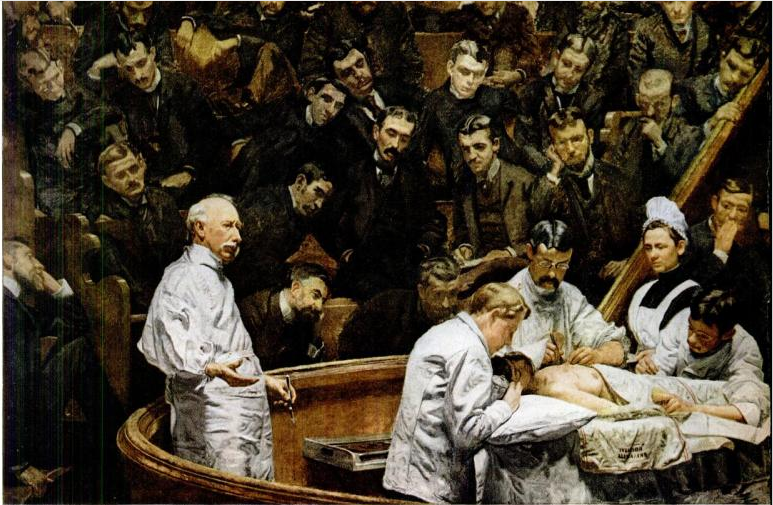
\includegraphics[width=\textwidth]{./images/agnewesclinic.png}\par}

{\centering \onelineheader{THE LATEX COUNTERS}\par}


The |File:m ltcounts.dtx| provides the command sequences defined by \latex to use with counters. It is a fairly short file with approximately 
60 lines of code. It is a good file to study in order to polish your skills in programming \tex. 

The heart of the counter commands are the \index{definecounter}

\index{LaTeX counters}
\index{LaTeX counters!\textbackslash setcounter}\index{LaTeX counters! \textbackslash addtocounter}\index{LaTeX counters! \textbackslash value}
The class starts with some definitions for |\setcounter|, |\addtocounter|, |\newcounter|, |\value|:


\begin{teXXX}
2 \def\setcounter#1#2{%
3   \@ifundefined{c@#1}%
4      {\@nocounterr{#1}}%
5      {\global\csname c@#1\endcsname#2\relax}}
\end{teXXX}


Testing for something here

Notice in line [5] that the name of the counter is prefixed with |c@|. This is automatically done for newcounter commands which we explain later on.


\index{LaTeX counters!\textbackslash newcounter}

\begin{docCommand}{newcounter}{}
The |\newcounter{newctr}[oldctr]| macro  Defines |newctr| to be a counter, which is
reset when counter |oldctr|  is stepped. If |newctr| is  already defined produces
|c@newctr already| defined  error.
\end{docCommand}

\begin{teXXX}
10 \def\newcounter#1{%
11   \expandafter\@ifdefinable \csname c@#1\endcsname
12   {\@definecounter{#1}}%
13   \@ifnextchar[{\@newctr{#1}}{}}
\end{teXXX}

The code checks to see, if an optional value is provided, using \cs{@ifnextchar} and branches to either
\cs{@definecounter} or to \cs{@newctr}. The two macros follow:

\begin{teXXX}
25 \def\@definecounter#1{\expandafter\newcount\csname c@#1\endcsname
26   \setcounter{#1}\z@
27   \global\expandafter\let\csname cl@#1\endcsname\@empty
28   \@addtoreset{#1}{@ckpt}%
29   \global\expandafter\let\csname p@#1\endcsname\@empty
30   \expandafter
31   \gdef\csname the#1\expandafter\endcsname\expandafter
32       {\expandafter\@arabic\csname c@#1\endcsname}
}
\end{teXXX}

\begin{docCommand}{@definecounter}{}
The command does a lot of work. Firstly, it defines a new counter using the \tex primitive \cmd{newcount} in line [25]. It then sets the counter using \cmd{setcounter} to zero (|\z@|). Lastly line [31], defines the counter as |thefoo|. This is an internal kernel command that provides the routines and definition of the counters to the rest of the macros.
\end{docCommand}

\begin{teXXX}
15 \def\@newctr#1[#2]{%
16   \@ifundefined{c@#2}{\@nocounterr{#2}}{\@addtoreset{#1}{#2}}}
\end{teXXX}




\begin{docCommand}{arabic} {}
Next follow a number of commands, for representing the values of counters in different forms, such
as arabic or roman numerals.
\end{docCommand}

\begin{teXXX}
34 \def\arabic#1{\expandafter\@arabic\csname c@#1\endcsname}
\end{teXXX}

\begin{docCommand}{roman} {}
\end{docCommand}
\begin{docCommand}{Roman}{}
\begin{docCommand}{alph}{}
\begin{docCommand}{Alph}{}
Representation of counter as lower-case Roman numerals. \cs{Roman} Representation of hcounteri as upper-case Roman numerals. \cs{alph} Representation of hcounteri as a lower-case letter: 1 = a, 2 = b, etc. \cs{Alph} Representation of hcounteri as an upper-case letter: 1 = A, 2 = B, etc.
The rest of the number definitions, follow in the same manner.  All of the commands, have internal macro representations. Of interest is the way |\Roman| is defined. The explanation follows after this block.

\end{docCommand}
\end{docCommand}
\end{docCommand}

\begin{teXXX}
35 \def\roman#1{\expandafter\@roman\csname c@#1\endcsname}
36 \def\Roman#1{\expandafter\@Roman\csname c@#1\endcsname}
37 \def\alph#1{\expandafter\@alph\csname c@#1\endcsname}
38 \def\Alph#1{\expandafter\@Alph\csname c@#1\endcsname}
\end{teXXX}

The internal representation, is straightforward:

\begin{teXXX}
\@arabic \@arabic\FOOcounter Representation of \FOOcounter as arabic numerals.
40 \def\@arabic#1{\number #1} %% changed 29 Apr 86
\@roman \@roman\FOOcounter Representation of \FOOcounter as lower-case Roman numerals.
41 \def\@roman#1{\romannumeral #1}
\@Roman \@Roman\FOOcounter Representation of \FOOcounter as upper-case Roman numerals.
42 \def\@Roman#1{\expandafter\@slowromancap\romannumeral #1@}
\end{teXXX}



\begin{teXXX}
\@slowromancap Fully expandable macro to change a roman number to uppercase.
43 \def\@slowromancap#1{\ifx @#1% then terminate
44 \else
45 \if i#1I\else\if v#1V\else\if x#1X\else\if l#1L\else\if
46 c#1C\else\if d#1D\else \if m#1M\else#1\fi\fi\fi\fi\fi\fi\fi
47 \expandafter\@slowromancap
48 \fi
49 }
\end{teXXX}



\makeatletter
\begin{teX}
\@slowromancap iiiv@ 
\end{teX}



\def\@Slowroman#1{\ifx @#1% then terminate
 \else
   \@fnsymbol#1 \texttt{\textbackslash @fnsymbol\{#1\}\\ } \expandafter\@Slowroman
 \fi
 }


\noindent \@Slowroman 123456789 @




\section{Footnote symbols}

\LaTeXe provides the \index{fnsymbol} command that holds the symbols for old fashioned footnote symbols. These can be used both in text or math mode. The definition is shown below.

\reflect{\@fnsymbol}
\bigskip


The symbols are as follows:

\noindent \@Slowroman 123456789 @


As it happens the \index{fnsymbol} is one of those commands that have been revised in \texttt{fixltx2e} \footnote{see \url{http://www.tex.ac.uk/tex-archive/macros/latex/unpacked/fixltx2e.sty}} and hence the definition shown is that of the \texttt{fixltx2e}.

\begin{teXX}
\ProvidesPackage{fixltx2e}

\def\@fnsymbol#1{%
   \ifcase#1\or \TextOrMath\textasteriskcentered *\or
   \TextOrMath \textdagger \dagger\or
   \TextOrMath \textdaggerdbl \ddagger \or
   \TextOrMath \textsection  \mathsection\or
   \TextOrMath \textparagraph \mathparagraph\or
   \TextOrMath \textbardbl \|\or
   \TextOrMath {\textasteriskcentered\textasteriskcentered}{**}\or
   \TextOrMath {\textdagger\textdagger}{\dagger\dagger}\or
   \TextOrMath {\textdaggerdbl\textdaggerdbl}{\ddagger\ddagger}\else
   \@ctrerr \fi
}

\end{teXX}

The old definition is shown below:

\begin{teXX}
58 \def\@fnsymbol#1{\ensuremath{\ifcase#1\or *\or \dagger\or \ddagger\or
59 \mathsection\or \mathparagraph\or \|\or **\or \dagger\dagger
60 \or \ddagger\ddagger \else\@ctrerr\fi}}
\end{teXX}

All nice and wonderfully, imaginative stuff that brings the discussion of the |ltcounts.dtx| to an end. This is one of the smaller classes, but important as counters are the heart of \latex. 



\index{stpelt}\index{LaTeX counters!\textbackslash stpelt}

This command takes one argument, a counter name and sets it to zero.

\begin{teXXX}
\@stpelt
23 \def\@stpelt#1{\global\csname c@#1\endcsname \z@}
\end{teXXX}


This can be used creatively in packages as for example the \docpkg{chappg}\footnote{numbers are from the chappg documentation} \footnote{see \url{http://www.tug.org/texlive/Contents/live/texmf-dist/doc/latex/chappg/chappg.pdf}}

\begin{teXXX}
The next magic makes the page counter be reset to one rather than zero
93 \renewcommand\@stpelt[1]{%
94 \global\csname c@#1\endcsname
95 \expandafter\ifx \csname c@#1\endcsname \c@page
96 \@ne
97 \else
98 \z@
99 \fi
100 }
\end{teXXX}



\texttt{\textbackslash cl@@ckpt}
\index{cl@@ckpt} is the  reset list of a dummy counter \index{ckpt}
used for taking checkpoints for the \cmd{include}\index{\textbackslash include} system.


\makeatletter
\def\@elt{,   }



\topline

{\footnotesize 
\cl@@ckpt 
}

\bottomline


\begin{teXX}
\cl@@ckpt
24 \def\cl@@ckpt{\@elt{page}}
\end{teXX}

\footnote{See also \url{http://www.tug.org/TUGboat/Articles/tb18-4/tb57work.pdf}}

The word \textit{elt}\index{elt} is short for element.


\begin{comment}
%This function returns the element of sequence indexed by index. Legitimate values of index are integers ranging from 0 up to one less than the length of sequence. If sequence is a list, then out-of-range values of index return nil; otherwise, they trigger an args-out-of-range error.
%
%\begin{verbatim} 	
%(elt [1 2 3 4] 2)
%=> 3
%\end{verbatim}
%\printindex 
%\end{document}
%
%\def\test#1{\def\res{#1}\ifx\foo\res True\\ \else Error \\ \fi}
%\edef\foo{\@car 123\@nil} \test{1}
%\edef\foo{\@car {1}23\@nil} \test{1}
%\edef\foo{\@car {123}{456}{7}\@nil} \test{123}
%\edef\foo{\@carcube1234567\@nil}\test{123}
%\edef\foo{\@cdr 123\@nil} \test{23}
%\edef\foo{\@cdr {134}{x}\@nil}   \test{x}
%\edef\foo{\@cdr {134}{{x}}\@nil} \test{{x}}
%
%\let\foo\@nnil \test{\@empty}
%
%
%
%\toks@={abc\foo}\addto@hook\toks@{x\bar}
%\expandafter\def\expandafter\foo\expandafter{\the\toks@} \test{abc\foo x\bar}
%\g@addto@macro\foo{y\gee} \test{abc\foo x\bar y\gee}
%\def\xx{456}
%\def\foo{123} \@cons\foo{\xx78}\test{123\@elt45678}
%
%
%
%http://www.tug.org/TUGboat/Articles/tb15-4/tb45braa.pdf
%
%
%

\end{comment}



%{ltmiscen.dtx}{flushleft}
%/{ltmiscen.dtx}{flushright}
%{ltmiscen.dtx}{center}

\section*{Introspection}
\index{Introspection}
In everyday life, introspection is the act of self-examination. Introspection refers to the examination of one's own thoughts, feelings, motivations, and actions. The great philosopher Socrates spent much of his life in self-examination, encouraging his fellow Athenians to do the same. He even claimed that, for him, "the unexamined life is not worth living." We can use some \tex trickery and \latex acrobatics to print the listing of a macro. We will call this macro \cmd{reflect}.\index{\textbackslash meaning}

\begin{teX}
\def\reflect{\@star@or@long\accommand}
\def\accommand#1{\string#1:%
  \expandafter\strip@prefix\meaning#1} 
\end{teX}

\noindent The definition appears deceptively simple (by having removed some cosmetic additions to format the output). Let us see as an example the output of |\reflect{\frogking}|.
\bigskip


\hfil\hfill Results of |\reflect{frogking}| 

\smallskip


\hrule
\medskip
\makeatletter
\def\showcommand{\@star@or@long\accommand}
\fboxrule=0.0pt
\def\accommand#1{\framebox[3cm][l]{\bf\color{red} 
    \string#1:~~} %
     \parbox[t]{7cm}{\expandafter\strip@prefix\meaning#1}} 
\showcommand*{\frogking}
\makeatother
\smallskip



\bigskip


The code captures both the name of the macro (strips the |macro:->| part and displays the definition). I did include some formatting commands to get it to display better.

If you have difficulty in understanding the code the best advice I can give you is to stop driving and take public transport. This applies to hackers as well as writers, but it may not be applied fully to mathematicians and physicists. If a typical commute is 30 minutes by car or 1 hour by public transportation, you may feel like you are losing an hour a day leaving your car at home, but you are actually gaining an hour of time if you bring your laptop, assuming you want to spend at least 2 hours a day working on things on your laptop outside work. Other upsides: cheaper, less stress, safer, better for the environment and you will get closer to understanding \tex.


\section*{Lisp relics in \protect\LaTeX\ }
\index{Lisp}
\newthought{Introduced in the Lisp programming language}, |car| and |cdr| are primitive operations upon linked lists composed of |cons cells| (or "non-atomic S-expressions"). A |cons cell| is composed of two pointers; the |car| operation extracts the first pointer, and the |cdr| operation extracts the second.
\index{S-expressions}
Thus, the expression |(car (cons x y))| evaluates to |x|, and |(cdr (cons x y))| evaluates to |y|.

When |cons| cells are used to implement singly-linked lists (rather than trees and other more complicated structures), the |car| operation returns the first element of the list, while cdr returns the rest of the list. For this reason, the operations are sometimes given the names first and rest or head and tail.

What does this have to do with \latex? Obviously the \latex authors knew their computer science well, as you can find many instances where these concepts are used. They are easily definable using \tex and the definitions can be found in the |ltdefn.dtx| file.

\begin{teX}
\def\@car#1#2\@nil{#1}
\def\@cdr#1#2\@nil{#2}
\@carcube \@carcube T1 ... Tn\@nil = T1 T2 T3 , n > 3
\def\@carcube#1#2#3#4\@nil{#1#2#3}
\end{teX}





\begin{teX}
%\LaTeXe The LATEX2" logo as proposed by A-W designers.
\makeatletter
 \def\LaTeXe{%
   \mbox{\m@th%
    \if b\expandafter\@car\f@series\@nil\boldmath\fi
     \LaTeX\kern.15em2$_{\textstyle\varepsilon}$}}
\makeatother
\end{teX}

\scalebox{5}{\LaTeXe}

To understand the command we first need to check the definition of |\m@th|, which defines the mathsurround to be equal to |\z@|. |\def\m@th{\mathsurround\z@}| \index{\textbackslash mathsurround}. So the first thing we did was to make sure that the space around the maths is set to zero. The strange setting is the |@car|, which picks up the first letter of |\boldmath|?

\makeatletter
\def\Latex{%
   \mbox{\m@th%
    %\if b\expandafter\@car\f@series\@nil\boldmath\fi
    \boldmath
     \LaTeX\kern.15em2$_{\textstyle\varepsilon}$}}
\makeatother

\scalebox{5}{\Latex}


Lisp was originally implemented on the IBM 704 computer, in the late 1950s. The 704 hardware had special support for splitting a 36-bit machine word into four parts, an "address part" and "decrement part" of 15 bits each and a "prefix part" and "tag part" of three bits each.

Precursors to Lisp included functions:

\begin{description}
\item{|car|} (short for "Contents of the Address part of Register number"),\index{car}
\item{|cdr|} ("Contents of the Decrement part of Register number"),\index{cdr}
\item{|cpr|} ("Contents of the Prefix part of Register number"), and\index{cpr}
\item{|ctr|} ("Contents of the Tag part of Register number"),\index{ctr}
\end{description}
each of which took a machine address as an argument, loaded the corresponding word from memory, and extracted the appropriate bits.















\chapter{The LateX Kernel}

\epigraph{He who would eat the kernel, must crack the shell.
[Lat., \textit{Qui e nuce nucleum esse vult, frangat nucem.}]}{Plautus}

\latex is the batteries of \tex. It has given authors the ability to write documents easily and in a consistent way. It has also provided pacakage writers with endless nights of work trying to figure out how things work. In this chapter we will describe briefly the workings of \latex and the areas where one could use it for improvements. The best source for how the \latex kernel works is \latex itself and the publication that comes with it \docFile{sourc2e.pdf}.

The original developer of \latex was Leslie Lamport. Lamport who is now a recipient of the Turing award, described his philosophy for document production in a paper \textit{Document Production: Visual or Logical?}, presented before the ACM in 1987. \parencite{lamport1987}

Although many developers have criticized the original code it is an amazing fact that it has endured. Although in today’s terms the system cannot be considered pluggable, it was
certainly extensible and the fact that \tex provides the means to write macros on the fly, the main effort
of the \latexe system was to provide the basic structure for the development of styles (now called classes).

The code was and is well documented and many of the comments are from the first system. I have spent many an
evening thinking that analyzing latex code, should be mandatory in modern computer classes to instill
good discipline in being economical with code and for discovering the right amount of abstraction before designing programming and delving into code.

\section{Code Organization.} 

The \latex source code is distributed in a number of |.dtx| files. These are saved in files |a|..|z| and files |A-O| The source files are documented in \docFile{source2e}, just |texdoc source2e| to read it. 

What I am describing here, is a step by step analysis of the kernel code, supplemented by additional materials, in order to provide an understanding of  the inner workings. 


\begin{longtable}{llp{5cm}}
\toprule
Filename  			 & Description & Reference\\
\midrule
\inc a ltxdirchk.dtx 	 & &      \\
\inc b ltplain.dtx    	 & & See Chapter \ref{kernel:ltplain}, page [\pageref{kernel:ltplain}]  \\
c ltvers.dtx     	 && Version information \ref{kernel:ltvers}      \\
d ltdefns.dtx     && See Chapter~\ref{ch:ltxdefns},pg~\pageref{ch:ltxdefns}\\
e ltalloc.dtx     && Allocations, Chapter \ref{kernel:ltalloc}, page [\pageref{kernel:ltalloc}] \\
f ltcntrl.dtx     && Control structures See Chapter~\ref{ch:ltcntrl}~\pageref{ch:ltcntrl}\\
g lterror.dtx     && Error handling  \pageref{kernel:lterror}\\ 
h ltpar.dtx      	 && Paragraphs See (\pageref{kernel:ltpar})\\
i ltspace.dtx		 && Spacing commands. See~Chapter \ref{kernel:ltspace}, page~[\pageref{kernel:ltspace}]\\
j ltlogos.dtx     && See \pageref{kernel:ltlogos}\\
k files.dtx			 && File handling, listing of files. See \pageref{kernel:ltfiles}\\
l ltoutenc.dtx    && Stadard encoding and commands See Chapter~\pageref{ltoutenc}\\
m ltcounts.dtx    && Chapter \ref{kernel:ltcounts}, page [\pageref{kernel:ltcounts}]\\
n ltlengths			 && Length setting commands. See~pg~[\pageref{kernel:lengths}]\\
o ltfssbas.dtx    && \pageref{kernel:ltfssbas}\\
p ltfsstrc.dtx    && Tracing fonts See Chapter~\pageref{kernel:ltfsstrc}\\
q ltfsscmp.dtx    && See Chapter \ref{kernel:ltfntcmd}, page [\pageref{kernel:ltfntcmd}] \\
s ltfssini.dtx    && NFSS Font initializaton, see Chapter~\ref{kernel:ltfssini}, page~\pageref{kernel:ltfssini}\\
t fontdef.dtx     && Chapter \ref{kernel:fontdef}, page [\pageref{kernel:fontdef}]\\ 
u preload.dtx     && Chapter \ref{kernel:preload} page [\pageref{kernel:preload}]\\
v ltfntcmd.dtx    && \pageref{kernel:ltfntcmd}\\
w ltpageno.dtx    && See Chapter \ref{kernel:ltpageno}, page [\pageref{kernel:ltpageno}]\\
x ltref.dtx       && See Chapter \ref{kernel:ltxref}, page [\pageref{kernel:ltxref}] \\
y ltmiscen.dtx    && See Chapter \ref{kernel:ltmiscen}, page [\pageref{kernel:ltmiscen}]\\
z ltmath.dtx      && See chapter \ref{kernel:ltmath}, page [\pageref{kernel:ltmath}]\\
A ltlists.dtx     && See \ref{kernel:ltlists}\\
B ltboxes.dtx     && See \pageref{kernel:ltboxes}\\
C lttab.dtx       && See \pageref{kernel:lttab}\\
D ltpictur.dtx    && See Chapter \ref{kernel:ltpictur}, page [\pageref{kernel:ltpictur}]\\
E ltthm.dtx       &Theorems& See Chapter \ref{kernel:ltthm}, page [\pageref{kernel:ltthm}]\\
F ltsect.dtx      &Sectioning& See \ref{kernel:ltsect} \\
G ltfloat.dtx     &Floats& See \ref{kernel:ltfloat}\\
H ltidxglo.dtx    &Indices \& Glossaries& See \pageref{kernel:ltidxglo}\\
I ltbibl.dtx      &Bibliography & See Chapter~\ref{kernel:biblio}, page [\pageref{kernel:biblio}]\\
J ltpage.dtx      && See Chapter\ref{kernel:ltpage}, page [\pageref{kernel:ltpage}]\\
K ltoutput.dtx    && \ref{kernel:ltoutput}\\
L ltclass.dtx     && See Chapter \ref{kernel:ltclass}, page [\pageref{kernel:ltclass}]\\
M lthyphen.dtx    && See Chapter \ref{kernel:lthyphen}, page [\pageref{kernel:lthyphen}]\\
N ltfinal.dtx     && See Chapter \ref{kernel:ltfinal}, page [\pageref{kernel:ltfinal}]\\
\bottomrule
\end{longtable}


\section{Autoloading}

When LaTeX2e was released, personal computers had much less power than nowadays. Moreover, TeX was often compiled with a rather small amount of available memory.
\footnote{\url{http://tex.stackexchange.com/questions/38436/what-is-autoload}}.

The inclusion of the New Font Selection Scheme (NFSS2), in particular, posed some challenges when LaTeXing big documents. So the developers provided a solution for people with limited memory available: if the autoload option was set during the extraction of latex.ltx from the sources, not all the kernel was included in the format which was then produced by running initex on this file: some parts of it were included "on demand", for instance the code for the picture environment.

Support of the autoload feature was introduced in the June 1995 release of the LaTeX kernel update and dropped in December 2003.

You can still find a description of this feature in the file

\begin{verbatim}
<TEX DIST ROOT>/doc/latex/base/autoload.txt
\end{verbatim}

On some small systems (perhaps most noticeably emTeX for PCs if your machine is unable to use the TeX386 version) LaTeX uses up a large amount of the memory available to TeX, leaving very little for storage of any further commands, complex text (such as tables), floats or cross references that may occur in a typical document. Note that these limits are built into the TeX executable and do not directly correspond to any physical memory that your machine has installed.

In order to help with this problem, we have produced an experimental configuration of LaTeX in which certain functions are not predefined in the format, but are loaded automatically from a style file the first time they are used. This saves a lot of memory in the case that a document does not use these features.

In this release two environments are ‘auto-loaded’ in this way, ‘picture’ and ‘tabbing’, as are various bits of internal code used in error handling, font loading and advanced page makeup.

  autopict.sty      source for picture mode
  autotabg.sty      source for tabbing environment
  autoerr.sty       texts of most LaTeX error commands
  autofss1.sty      little used internal font selection commands
  autoout1.sty      source for \cs{enlargethispage} and related commands.

\makeatletter

\section{File a ltdirchk.dtx}

This file implements the semi-automatic determination of various system dependent
parts of the initialisation. The actual definitions may be placed in a file
|texsys.cfg|. Thus for operating systems for which the tests here do not result in
acceptable settings, a `hand written' texsys.cfg may be produced.
Current directoty \cs{@currdir}.


|\input@path| For most common operating sytsems is let to undefined. % undefined on window

The routines define a useful macro to parse file name paths:

\begin{texexample}{Parsing directories}{ex:directories}
\filename@parse{./test/some other paths/path/tex.jpg}

\filename@area

\filename@base,

\filename@ext

\end{texexample}

The |\@TeXversion| is only defined for very old versions of |TeX|, on a reasonable modern distribution, it should be let to undefined.



\section{File k ltfiles.dtx}


\begin{tabular}{lp{5cm}}
|\document| &\\
|\nofiles| &\\
|\includeonly| &\\
|\include| &\\
|\input| &\\
|ifFileExists| &\\
|\InputIfFileExists| & If the file exists on a system, execute then input the name, otherwise execute \textit{else}\\
\end{tabular}





\section{Listing files}  

A list of files so far. The initial value of |@gobble| eats the comma before the first file name. Here we start encountering \LaTeX's iteration macros:

The |\@filelist| is a comma delimited list that will hold the value of all files. It is let to |\@gobble| in order to eat the first comma. This is a nifty trick. 

\begin{teX}
204 \let\@filelist\@gobble
\end{teX}

The next macro adds a file name to the list. If you are not familiar with lists this is an interestin way of understanding, how a comma delimited list is build.

\begin{teXXX}
205 \def\@addtofilelist#1{\xdef\@filelist{\@filelist,#1}}
\end{teXXX}

Note that the |\@filelist| gets deactivated if |\listfiles| does not appear in the preamble. The |begin{document}|
contains code equivalent to:

\begin{teXXX}
\AtBeginDocument{%
  \ifx\@listfiles\@undefined
  \let\@filelist\relax
  \let\@addtofilelist\@gobble
\fi}
\@onlypreamble\listfiles
\let\@dofilelist\relax
\end{teXXX} 
\index{onlypreamble}



\section{Version name and version date \texttt{File c ltvers.dtx.}}

\begin{docCommand}{fmtname}{}
LaTeXe's name is stored here as LaTeX2e
\end{docCommand}

\begin{docCommand}{fmtversion}{}
prints the format version
\end{docCommand}

This is a small class,  that its sole purpose is to provide version information. It checks
if the format is too old. If it is older than 65 months it emits an error. 

\begin{teXXX}
2 \def\fmtname{LaTeX2e}
3 \edef\fmtversion{2011/06/27}
\end{teXXX}

After the format version is hardcoded, a macro using one of LaTeX's scratch names is defined. The parameters
of this macro are delimited in the same way as the date in the format version definition, thus a comparison can be made between the two periods. If it is longer than a preset period it emits an error.

\begin{teXXX}
4 \iffalse
5 \def\reserved@a#1/#2/#3\@nil{%
6   \count@\year
7   \advance\count@-#1\relax
8   \multiply\count@ by 12\relax
9   \advance\count@\month
10 \advance\count@-#2\relax}
11 \expandafter\reserved@a\fmtversion\@nil
12 \ifnum\count@>65
13     \typeout{^^J%
14     !!!!!!!!!!!!!!!!!!!!!!!!!!!!!!!!!!!!!!!!!!!!!!!^^J%
15     ! You are attempting to make a LaTeX format from a source file^^J%
16     ! That is more than five years old.^^J%
17     !^^J%
18     ! If you enter <return> to scroll past this message then the format^^J%
19     ! will be built, but please consider obtaining newer source files^^J%
20     ! before continuing to build LaTeX.^^J%
21     !!!!!!!!!!!!!!!!!!!!!!!!!!!!!!!!!!!!!!!!!!!!!!!!^^J%
22     }
23     \errhelp{To avoid this error message, obtain new LaTeX sources.}
24     \errmessage{LaTeX source files more than 5 years old!}
25 \fi
26 \let\reserved@a\relax
27 \fi
\end{teXXX}

It does not appear that this macro is currently activated, but I can be wrong. One cannot help but notice the conservatism in saving memory by the use of nameless scratch macros. Good practice dictates, that after their use they are let to |\relax|.

\begin{texexample}{}{}
\fmtname  [\fmtversion]
\end{texexample}


\section{File d ltplain.dtx}

The routines covered by this file go deep into the heart of the kernel. Besides storing some of the plain commands in new macros, this section of the kernel defines its own defining commands like |\newcommand|, |\newenvironment| and similar other macros. We start by summarizing the author and internal commands available in this section.


\section{File  Bibliographies ltbibl.dtx} 

A bibliography is created by the \cmd{thebibliography} environment, which generates
a title such as "References", and a list of entries. The \texttt{BIBTEX} program will create
a file containing such an environment, which will be read in by the \cmd{bibliography}
command. With BIBTEX, the following commands will be used


\cmd{bibliography} This commands reads in all the filenames of the bibliography. |\bibliography{file1,file2,file3,file4}|
It will then write a \cmd{bibdata} entry on the |.aux| file and tries to read in |mainfile.bbl|.


\begin{teX}
\def\bibliography#1{%
 \if@filesw
 \immediate\write\@auxout{\string\bibdata{#1}}%
 \fi
 \@input@{\jobname.bbl}
}
\end{teX}

The \cmd{if@filesw} is defined in File k (ltfiles.dtx) as follows:
\begin{teX}
\newif\if@filesw \@fileswtrue
\end{teX}

The |bibliograhy| command simply writes the |bibdata|. Notice that |\string| is used to make sure  there is no expansion. \cmd{@input@} is a version of \cmd{@input} that does add the file to \cmd{@filelist}. This is also defined in |ltfiles.dtx|. 

\begin{teX}
\def\@input@#1{\InputIfFileExists{#1}{}{\typeout{No file #1.}}}
\end{teX}


\noindent It simply checks if the file exists and outputs to 

\startlineat{32}
\begin{teX}
 \def\bibliographystyle#1{%
 \ifx\@begindocumenthook\@undefined\else
   \expandafter\AtBeginDocument
 \fi
 {\if@filesw
  \immediate\write\@auxout{\string\bibstyle{#1}}%
 \fi}}
\end{teX}





The bibliography environment is a list environment. Instead of using |\item|, it uses \cmd{bibitem}. The rest of the commands are \cmd{cite} and \cmd{nocite}.

The \cmd{nocite}, puts information on the |.aux| file that causes |\bibtex| to include a citation list in the bibliography, but nothing in the document.\cmd{nocite\{*\}} is special it tells |\bibtex| to put the whole of a collection of citation with comment.
references into the bibiography.

Most of the Bibliography formatting comes later in the actual classes.


\cmd{if@tempswa} General boolean switch used by LATEX kernel commands.
defines as |\newif\if@tempswa|

The \cmd{@cite} hook determines the \textit{relative formatting} of the two logical parts of a citation

\begin{teX}
\def\@cite#1#2{[{#1\if@tempswa , #2\fi}]}
\end{teX}


Not the easiest of read and the whole think should have a rethink for better modularity.



\section{parboxes and other boxed things!}

\label{parbox}\index{parbox}\index{mode!paragraph}
A \cmd{parbox} is a box whose contents are created in paragraph mode. The |\parbox| has two mandatory arguments:

\begin{teX}
\parbox[position][height][inner-pos]{width}{text}
\end{teX}

\noindent For example,

\begin{teX}
\parbox{7cm}{\onepar}
\end{teX}

\noindent\parbox{7cm}{\onepar}

\bigskip

\begin{description}
\item[width]  specifies the width of the parbox, and
\item[text]   the text that goes inside the parbox.
\end{description}


\latex will position a parbox so its centre lines up with the centre of the text line. The optional position argument allows you to line up either the top or bottom line in the parbox (default is top).

If the height argument is not given, the box will have the natural height of the text.

The [inner-pos] argument controls the placement of the text inside the box. If it is not specified, position is used.

\begin{enumerate}
\item[t]  text is placed at the top of the box.
\item[c]  text is centred in the box.
\item[b]  text is placed at the bottom of the box.
\item[s]  stretch vertically. The text must contain vertically stretchable space for this to work.
\end{enumerate}

A parbox command is used for a parbox containing a small piece of text, with nothing fancy inside. In particular, you shouldn't use any of the paragraph-making environments inside a parbox argument. For larger pieces of text, including ones containing a paragraph-making environment, you should use a \cs{minipage} environment 

\begin{teX}
\def\parbox{%
  \@ifnextchar[%]
   \@iparbox
   {\@iiiparbox c\relax[s]}}
\end{teX}

The definition of the user command |\parbox| is quite simple and follows the typical pattern found with \latex commands. The macro, uses the |@ifnextcharacter|, to check for a left square bracket ([), to check if an optional argument has been supplied or not. If one was supplied |@iiiparbox| is called else
|\@iiparbox| is called. This is typical of many \latex commands, where optional arguments are supplied. Four macros are used to provide a user command. The command, in this case |\parbox| and |@iparbox|, |@iiparbox| and |@iiiparbox|. The real work (in the case of |\parbox| is undertaken by the internal command |@iiiparbox|. It takes some time to get used to these patterns and my suggestion is for you to try a few macros for practice, plus read this chapter a couple of times trying some of the examples.

The \index{iparbox} just handles the case again of optional arguments,

\begin{teX}
\def\@iparbox[#1]{%
   \@ifnextchar[%]
   {\@iiparbox{#1}}%
   {\@iiiparbox{#1}\relax[s]}}
\end{teX}


  

\begin{teX}
\def\@iiparbox#1[#2]{%
   \@ifnextchar[%]
   {\@iiiparbox{#1}{#2}}%
   {\@iiiparbox{#1}{#2}[#1]}}
\end{teX}

\begin{teX}
   \let\@parboxto\@empty
\end{teX}

\hspace{-1cm}\texttt{\textbackslash @iiiparbox}

The internal version of \texttt{\textbackslash parbox}. The parameter text is as follows:

\begin{verbatim}
#1 position t, b (default is top)
#2 height
#3 inner position t, c, b, c
#4 width
#5 text
\end{verbatim}

\begin{teX}
  \long\def\@iiiparbox#1#2[#3]#4#5{%
    \leavevmode
    \@pboxswfalse
    \setlength\@tempdima{#4}%
    \@begin@tempboxa\vbox{\hsize\@tempdima\@parboxrestore#5\@@par}%
     %check height 
     \ifx\relax#2\else %empty
        \setlength\@tempdimb{#2}%set to height
        \edef\@parboxto{to\the\@tempdimb}%
        \fi
      \if#1b\vbox
        \else\if #1t\vtop
          \else\ifmmode\vcenter
            \else\@pboxswtrue $\vcenter
      \fi\fi\fi
      %set parbox (originally defined as empty) 
      \@parboxto{\let\hss\vss\let\unhbox\unvbox
        \csname bm@#3\endcsname}%
      \if@pboxsw \m@th$\fi
    \@end@tempboxa}
\end{teX}

\noindent The \cmd{bm@} takes various values and is used for spacing. 
|\bm@l|, |\bm@r|, |\bm@s|, |\bm@t|, |\bm@b|


\textbf{Set up spacing}

\startlineat{21}
\begin{teX}
  \def\bm@c{\hss\unhbox\@tempboxa\hss}
  \def\bm@l{\unhbox\@tempboxa\hss}\let\bm@t\bm@l
  \def\bm@r{\hss\unhbox\@tempboxa}\let\bm@b\bm@r
  \def\bm@s{\unhbox\@tempboxa}
\end{teX}


\noindent If you are wondering what |\@pboxswfalse| and |\@pboxswtrue| you can checkit out by using \cmd{meaning}. There is also the package \docpkg{reflex} which you can use.

\endinput

\makeatletter

\parindent0pt

\def\reflect{\@star@or@long\accommand}
\fboxrule=0.0pt

\long\def\accommand#1{\framebox[4cm][l]{%
     {\tt\string#1 \hfill:}} %
     \parbox[t]{7cm}{\tt\expandafter\strip@prefix\meaning#1}} 


%% Must change to minipage
\def\ccommand#1{\parbox[t]{4cm}{\string#1}\parbox[t]{7cm}{#1}}


\reflect{\bm@c}

\reflect{\@pboxswtrue}

\reflect{\@pboxswtrue}

\reflect{\leavevmode}


\meaning\@@par

\meaning\hss

\meaning\ifmmode

\meaning\vbox

\meaning\voidb@x

\def\texprim{\texttt{\protect\TeX\ primitive}}

\begin{comment}

\def\CMhss{Glue that is infinitely stretchable as well as infinitely strechable \texprim}

\def\CMi{The \BS i command is valid in math mode and text mode. It generates an i without dot (Unicode U+131, \i). The \BS I command expands to I, but is converted to \BS i by \BS MakeLowercase. \texprim}


\ccommand{\CMi}

\reflect{\CMhss}

\reflect{\CMi}

\CMi

\if{\meaning\par}{\meaning\par}{True} \else {false}

\ifx{\par\meaning}{\meaning\par}{True}\else{false}


\end{comment}


To complete the code the \cmd{\@arrayparboxrestore} is defined. This  restores various paragraph parameters. The rational for allowing two normally global 
flags to be set locally here was stated originally by Donald Arsenau and extended by Chris Rowley. It is because these  flags are only set globally to true by section commands, and these should
never appear within boxes or, indeed, in any group; and they are only ever set globally to false when they are definitely true.
File B: ltboxes.dtx Date: 2006/05/18 Version v1.1g 237
If anyone is unhappy with this argument then both 
flags should be treated as in |\set@nobreak|; otherwise this command will be redundant.

\begin{teXX}
176 \def\@arrayparboxrestore{%
177 \let\if@nobreak\iffalse
178 \let\if@noskipsec\iffalse
179 \let\par\@@par
180 \let\-\@dischyph
\end{teXX}

Redefined accents to allow changes in font encoding
\begin{teXX}
181 \let\'\@acci\let\`\@accii\let\=\@acciii
182 \parindent\z@ \parskip\z@skip
183 \everypar{}%
184 \linewidth\hsize
185 \@totalleftmargin\z@
186 \leftskip\z@skip \rightskip\z@skip \@rightskip\z@skip
187 \parfillskip\@flushglue \lineskip\normallineskip
188 \baselineskip\normalbaselineskip
189 \sloppy}
\end{teXX}

Finally the \cmd{parboxrestore} restores various paragraph parameters, and also |\\|.

\begin{teXX}
190 \def\@parboxrestore{\@arrayparboxrestore\let\\\@normalcr}
\end{teXX}


\makeatletter
{\obeylines
\meaning\if@nobreak
\meaning\if@noskipsec
\meaning\@dischyph
\meaning\discretionary
}
\makeatother

The code between \cmd{\@begin@tempboxa} are helper macros for supporting \cmd{height}, \cmd{width} etc. It grabs \#1 into \index{@tempboxa} and measures it. It also allows for macros involved with the coloring of the box.


This was a long write and possibly a long read. As \latex was written a long time ago. One could improve the user interface of the command by
defining the |\parbox| with the |keyval| package. Will it be more intuitive to describe

\begin{teXX}
\parboX[width=7cm, 
        height=8cm,
        textposition=t, 
        outerposition=b]{teX}
\end{teXX}

\section*{Strip the backslash}

\tex's possibilities are almost infinite. Here is another example of
an argument that is thrown away\cite{amy1990}, that just strips the backslash:

\begin{teXXX}
\def\stripbackslash#1#2*{\def\one{#2}}
\end{teXXX}

which only uses the second argument, throwing away the
first argument, in this case stripping away a backslash
from a control sequence supplied by the user. \cmd{stripbackslash}
can then be used in another macro which
needs a control sequence without its backslash to work
correctly, for instance:

\begin{texexample}{Stripping a backslash}{}
\def\stripbackslash#1#2*{\def\one{#2}}
\def\newdef#1{\expandafter
\stripbackslash\string#1* \one}

\newdef\testmacro
\end{texexample}



Instead of simply printing the control sequence without
the backslash, |\newdef| can be rewritten to test to see
if a given macro has already been defined. In this example,
|\newdef| tests to see if the expansion of the control
sequence |\csname\one\endcsname|, (where |\one|,
was defined by |\stripbackslash| to be the control sequence
supplied by the user minus its backslash) is equal
to |\relax|. This takes advantage of the TEX convention
that a previously undefined control sequence invoked in
a |\csname...\endcsname| environment will be understood
to be equal to |\relax|, whereas an already defined
control sequence will not:

\begin{texexample}{A command to define commands}{}
\def\newdef#1{%
  \expandafter\stripbackslash\string#1*
  %% \stripbackslash defines \one
  \expandafter
  \ifx\csname\one\endcsname\relax
      %% \one is expanded to be the
      %% control sequence the user supplied
      %% minus the backslash.
      %% If csname construction equals
      %% \relax, do nothing
  \else %% Else, give error message:
    {\tt Sorry, \string#1 has already been
     defined. Please supply a new name.}
\fi}
\end{texexample}


\chapter{\LaTeX counters}

\thispagestyle{plain}
{\centering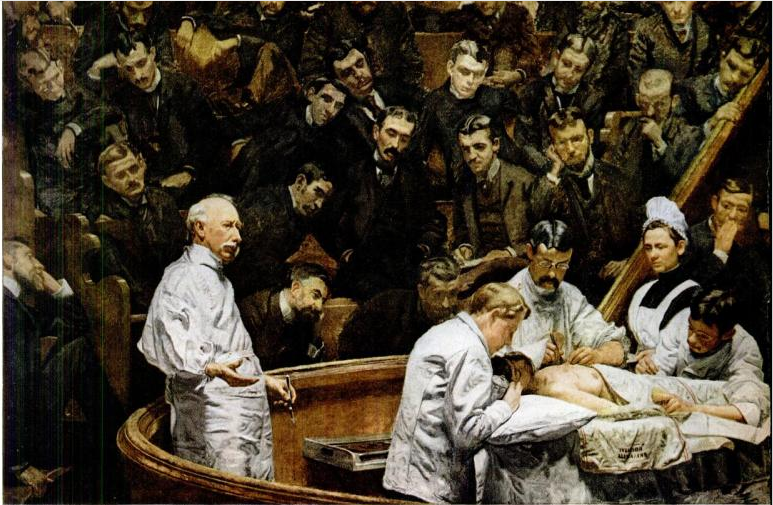
\includegraphics[width=\textwidth]{./images/agnewesclinic.png}\par}

{\centering \onelineheader{THE LATEX COUNTERS}\par}


The |File:m ltcounts.dtx| provides the command sequences defined by \latex to use with counters. It is a fairly short file with approximately 
60 lines of code. It is a good file to study in order to polish your skills in programming \tex. 

The heart of the counter commands are the \index{definecounter}

\index{LaTeX counters}
\index{LaTeX counters>\textbackslash setcounter}\index{LaTeX counters>\textbackslash addtocounter}\index{LaTeX counters>\textbackslash value}
The class starts with some definitions for |\setcounter|, |\addtocounter|, |\newcounter|, |\value|:


\begin{teXXX}
2 \def\setcounter#1#2{%
3   \@ifundefined{c@#1}%
4      {\@nocounterr{#1}}%
5      {\global\csname c@#1\endcsname#2\relax}}
\end{teXXX}


Testing for something here

Notice in line [5] that the name of the counter is prefixed with |c@|. This is automatically done for newcounter commands which we explain later on.


\index{LaTeX counters!\textbackslash newcounter}

\begin{docCommand}{newcounter}{}
The |\newcounter{newctr}[oldctr]| macro  Defines |newctr| to be a counter, which is
reset when counter |oldctr|  is stepped. If |newctr| is  already defined produces
|c@newctr already| defined  error.
\end{docCommand}

\begin{teXXX}
10 \def\newcounter#1{%
11   \expandafter\@ifdefinable \csname c@#1\endcsname
12   {\@definecounter{#1}}%
13   \@ifnextchar[{\@newctr{#1}}{}}
\end{teXXX}

The code checks to see, if an optional value is provided, using \cs{@ifnextchar} and branches to either
\cs{@definecounter} or to \cs{@newctr}. The two macros follow:

\begin{teXXX}
25 \def\@definecounter#1{\expandafter\newcount\csname c@#1\endcsname
26   \setcounter{#1}\z@
27   \global\expandafter\let\csname cl@#1\endcsname\@empty
28   \@addtoreset{#1}{@ckpt}%
29   \global\expandafter\let\csname p@#1\endcsname\@empty
30   \expandafter
31   \gdef\csname the#1\expandafter\endcsname\expandafter
32       {\expandafter\@arabic\csname c@#1\endcsname}
}
\end{teXXX}

\begin{docCommand}{@definecounter}{}
The command does a lot of work. Firstly, it defines a new counter using the \tex primitive \cmd{newcount} in line [25]. It then sets the counter using \cmd{setcounter} to zero (|\z@|). Lastly line [31], defines the counter as |thefoo|. This is an internal kernel command that provides the routines and definition of the counters to the rest of the macros.
\end{docCommand}

\begin{teXXX}
15 \def\@newctr#1[#2]{%
16   \@ifundefined{c@#2}{\@nocounterr{#2}}{\@addtoreset{#1}{#2}}}
\end{teXXX}

\endinput

\begin{docCommand}{arabic} {}
Next follow a number of commands, for representing the values of counters in different forms, such
as arabic or roman numerals.
\end{docCommand}

\begin{teXXX}
34 \def\arabic#1{\expandafter\@arabic\csname c@#1\endcsname}
\end{teXXX}

\begin{docCommand}{roman} {}
\end{docCommand}
\begin{docCommand}{Roman}{}
\begin{docCommand}{alph}{}
\begin{docCommand}{Alph}{}
Representation of counter as lower-case Roman numerals. \cs{Roman} Representation of hcounteri as upper-case Roman numerals. \cs{alph} Representation of hcounteri as a lower-case letter: 1 = a, 2 = b, etc. \cs{Alph} Representation of hcounteri as an upper-case letter: 1 = A, 2 = B, etc.
The rest of the number definitions, follow in the same manner.  All of the commands, have internal macro representations. Of interest is the way |\Roman| is defined. The explanation follows after this block.

\end{docCommand}
\end{docCommand}
\end{docCommand}

\begin{teXXX}
35 \def\roman#1{\expandafter\@roman\csname c@#1\endcsname}
36 \def\Roman#1{\expandafter\@Roman\csname c@#1\endcsname}
37 \def\alph#1{\expandafter\@alph\csname c@#1\endcsname}
38 \def\Alph#1{\expandafter\@Alph\csname c@#1\endcsname}
\end{teXXX}

The internal representation, is straightforward:

\begin{teXXX}
\@arabic \@arabic\FOOcounter Representation of \FOOcounter as arabic numerals.
40 \def\@arabic#1{\number #1} %% changed 29 Apr 86
\@roman \@roman\FOOcounter Representation of \FOOcounter as lower-case Roman numerals.
41 \def\@roman#1{\romannumeral #1}
\@Roman \@Roman\FOOcounter Representation of \FOOcounter as upper-case Roman numerals.
42 \def\@Roman#1{\expandafter\@slowromancap\romannumeral #1@}
\end{teXXX}



\begin{teXXX}
\@slowromancap Fully expandable macro to change a roman number to uppercase.
43 \def\@slowromancap#1{\ifx @#1% then terminate
44 \else
45 \if i#1I\else\if v#1V\else\if x#1X\else\if l#1L\else\if
46 c#1C\else\if d#1D\else \if m#1M\else#1\fi\fi\fi\fi\fi\fi\fi
47 \expandafter\@slowromancap
48 \fi
49 }
\end{teXXX}



\makeatletter
\begin{teX}
\@slowromancap iiiv@ 
\end{teX}



\def\@Slowroman#1{\ifx @#1% then terminate
 \else
   \@fnsymbol#1 \texttt{\textbackslash @fnsymbol\{#1\}\\ } \expandafter\@Slowroman
 \fi
 }


\noindent \@Slowroman 123456789 @




\section{Footnote symbols}

\LaTeXe provides the \index{fnsymbol} command that holds the symbols for old fashioned footnote symbols. These can be used both in text or math mode. The definition is shown below.

\reflect{\@fnsymbol}
\bigskip


The symbols are as follows:

\noindent \@Slowroman 123456789 @


As it happens the \index{fnsymbol} is one of those commands that have been revised in \texttt{fixltx2e} \footnote{see \url{http://www.tex.ac.uk/tex-archive/macros/latex/unpacked/fixltx2e.sty}} and hence the definition shown is that of the \texttt{fixltx2e}.

\begin{teXX}
\ProvidesPackage{fixltx2e}

\def\@fnsymbol#1{%
   \ifcase#1\or \TextOrMath\textasteriskcentered *\or
   \TextOrMath \textdagger \dagger\or
   \TextOrMath \textdaggerdbl \ddagger \or
   \TextOrMath \textsection  \mathsection\or
   \TextOrMath \textparagraph \mathparagraph\or
   \TextOrMath \textbardbl \|\or
   \TextOrMath {\textasteriskcentered\textasteriskcentered}{**}\or
   \TextOrMath {\textdagger\textdagger}{\dagger\dagger}\or
   \TextOrMath {\textdaggerdbl\textdaggerdbl}{\ddagger\ddagger}\else
   \@ctrerr \fi
}

\end{teXX}

The old definition is shown below:

\begin{teXX}
58 \def\@fnsymbol#1{\ensuremath{\ifcase#1\or *\or \dagger\or \ddagger\or
59 \mathsection\or \mathparagraph\or \|\or **\or \dagger\dagger
60 \or \ddagger\ddagger \else\@ctrerr\fi}}
\end{teXX}

All nice and wonderfully, imaginative stuff that brings the discussion of the |ltcounts.dtx| to an end. This is one of the smaller classes, but important as counters are the heart of \latex. 



\index{stpelt}\index{LaTeX counters!\textbackslash stpelt}

This command takes one argument, a counter name and sets it to zero.

\begin{teXXX}
\@stpelt
23 \def\@stpelt#1{\global\csname c@#1\endcsname \z@}
\end{teXXX}


This can be used creatively in packages as for example the \docpkg{chappg}\footnote{numbers are from the chappg documentation} \footnote{see \url{http://www.tug.org/texlive/Contents/live/texmf-dist/doc/latex/chappg/chappg.pdf}}

\begin{teXXX}
The next magic makes the page counter be reset to one rather than zero
93 \renewcommand\@stpelt[1]{%
94 \global\csname c@#1\endcsname
95 \expandafter\ifx \csname c@#1\endcsname \c@page
96 \@ne
97 \else
98 \z@
99 \fi
100 }
\end{teXXX}



\texttt{\textbackslash cl@@ckpt}
\index{cl@@ckpt} is the  reset list of a dummy counter \index{ckpt}
used for taking checkpoints for the \cmd{include}\index{\textbackslash include} system.


\makeatletter
\def\@elt{,   }



\topline

{\footnotesize 
\cl@@ckpt 
}

\bottomline


\begin{teXX}
\cl@@ckpt
24 \def\cl@@ckpt{\@elt{page}}
\end{teXX}

\footnote{See also \url{http://www.tug.org/TUGboat/Articles/tb18-4/tb57work.pdf}}

The word \textit{elt}\index{elt} is short for element.


\begin{comment}
%This function returns the element of sequence indexed by index. Legitimate values of index are integers ranging from 0 up to one less than the length of sequence. If sequence is a list, then out-of-range values of index return nil; otherwise, they trigger an args-out-of-range error.
%
%\begin{verbatim} 	
%(elt [1 2 3 4] 2)
%=> 3
%\end{verbatim}
%\printindex 
%\end{document}
%
%\def\test#1{\def\res{#1}\ifx\foo\res True\\ \else Error \\ \fi}
%\edef\foo{\@car 123\@nil} \test{1}
%\edef\foo{\@car {1}23\@nil} \test{1}
%\edef\foo{\@car {123}{456}{7}\@nil} \test{123}
%\edef\foo{\@carcube1234567\@nil}\test{123}
%\edef\foo{\@cdr 123\@nil} \test{23}
%\edef\foo{\@cdr {134}{x}\@nil}   \test{x}
%\edef\foo{\@cdr {134}{{x}}\@nil} \test{{x}}
%
%\let\foo\@nnil \test{\@empty}
%
%
%
%\toks@={abc\foo}\addto@hook\toks@{x\bar}
%\expandafter\def\expandafter\foo\expandafter{\the\toks@} \test{abc\foo x\bar}
%\g@addto@macro\foo{y\gee} \test{abc\foo x\bar y\gee}
%\def\xx{456}
%\def\foo{123} \@cons\foo{\xx78}\test{123\@elt45678}
%
%
%
%http://www.tug.org/TUGboat/Articles/tb15-4/tb45braa.pdf
%
%
%

\end{comment}



%{ltmiscen.dtx}{flushleft}
%/{ltmiscen.dtx}{flushright}
%{ltmiscen.dtx}{center}

\section*{Introspection}
\index{Introspection}
In everyday life, introspection is the act of self-examination. Introspection refers to the examination of one's own thoughts, feelings, motivations, and actions. The great philosopher Socrates spent much of his life in self-examination, encouraging his fellow Athenians to do the same. He even claimed that, for him, "the unexamined life is not worth living." We can use some \tex trickery and \latex acrobatics to print the listing of a macro. We will call this macro \cmd{reflect}.\index{\textbackslash meaning}

\begin{teX}
\def\reflect{\@star@or@long\accommand}
\def\accommand#1{\string#1:%
  \expandafter\strip@prefix\meaning#1} 
\end{teX}

\noindent The definition appears deceptively simple (by having removed some cosmetic additions to format the output). Let us see as an example the output of |\reflect{\frogking}|.
\bigskip


\hfil\hfill Results of |\reflect{frogking}| 

\smallskip


\hrule
\medskip
\makeatletter
\def\showcommand{\@star@or@long\accommand}
\fboxrule=0.0pt
\def\accommand#1{\framebox[3cm][l]{\bf\color{red} 
    \string#1:~~} %
     \parbox[t]{7cm}{\expandafter\strip@prefix\meaning#1}} 
\showcommand*{\frogking}
\makeatother
\smallskip



\bigskip


The code captures both the name of the macro (strips the |macro:->| part and displays the definition). I did include some formatting commands to get it to display better.

If you have difficulty in understanding the code the best advice I can give you is to stop driving and take public transport. This applies to hackers as well as writers, but it may not be applied fully to mathematicians and physicists. If a typical commute is 30 minutes by car or 1 hour by public transportation, you may feel like you are losing an hour a day leaving your car at home, but you are actually gaining an hour of time if you bring your laptop, assuming you want to spend at least 2 hours a day working on things on your laptop outside work. Other upsides: cheaper, less stress, safer, better for the environment and you will get closer to understanding \tex.


\section*{Lisp relics in \protect\LaTeX\ }
\index{Lisp}
\newthought{Introduced in the Lisp programming language}, |car| and |cdr| are primitive operations upon linked lists composed of |cons cells| (or "non-atomic S-expressions"). A |cons cell| is composed of two pointers; the |car| operation extracts the first pointer, and the |cdr| operation extracts the second.
\index{S-expressions}
Thus, the expression |(car (cons x y))| evaluates to |x|, and |(cdr (cons x y))| evaluates to |y|.

When |cons| cells are used to implement singly-linked lists (rather than trees and other more complicated structures), the |car| operation returns the first element of the list, while cdr returns the rest of the list. For this reason, the operations are sometimes given the names first and rest or head and tail.

What does this have to do with \latex? Obviously the \latex authors knew their computer science well, as you can find many instances where these concepts are used. They are easily definable using \tex and the definitions can be found in the |ltdefn.dtx| file.

\begin{teX}
\def\@car#1#2\@nil{#1}
\def\@cdr#1#2\@nil{#2}
\@carcube \@carcube T1 ... Tn\@nil = T1 T2 T3 , n > 3
\def\@carcube#1#2#3#4\@nil{#1#2#3}
\end{teX}





\begin{teX}
%\LaTeXe The LATEX2" logo as proposed by A-W designers.
\makeatletter
 \def\LaTeXe{%
   \mbox{\m@th%
    \if b\expandafter\@car\f@series\@nil\boldmath\fi
     \LaTeX\kern.15em2$_{\textstyle\varepsilon}$}}
\makeatother
\end{teX}

\scalebox{5}{\LaTeXe}

To understand the command we first need to check the definition of |\m@th|, which defines the mathsurround to be equal to |\z@|. |\def\m@th{\mathsurround\z@}| \index{\textbackslash mathsurround}. So the first thing we did was to make sure that the space around the maths is set to zero. The strange setting is the |@car|, which picks up the first letter of |\boldmath|?

\makeatletter
\def\Latex{%
   \mbox{\m@th%
    %\if b\expandafter\@car\f@series\@nil\boldmath\fi
    \boldmath
     \LaTeX\kern.15em2$_{\textstyle\varepsilon}$}}
\makeatother

\scalebox{5}{\Latex}


Lisp was originally implemented on the IBM 704 computer, in the late 1950s. The 704 hardware had special support for splitting a 36-bit machine word into four parts, an "address part" and "decrement part" of 15 bits each and a "prefix part" and "tag part" of three bits each.

Precursors to Lisp included functions:

\begin{description}
\item{|car|} (short for "Contents of the Address part of Register number"),\index{car}
\item{|cdr|} ("Contents of the Decrement part of Register number"),\index{cdr}
\item{|cpr|} ("Contents of the Prefix part of Register number"), and\index{cpr}
\item{|ctr|} ("Contents of the Tag part of Register number"),\index{ctr}
\end{description}
each of which took a machine address as an argument, loaded the corresponding word from memory, and extracted the appropriate bits.















% \iffalse meta-comment
%
% Copyright 1993-2017
% The LaTeX3 Project and any individual authors listed elsewhere
% in this file.
%
% This file is part of the LaTeX base system.
% -------------------------------------------
%
% It may be distributed and/or modified under the
% conditions of the LaTeX Project Public License, either version 1.3c
% of this license or (at your option) any later version.
% The latest version of this license is in
%    http://www.latex-project.org/lppl.txt
% and version 1.3c or later is part of all distributions of LaTeX
% version 2005/12/01 or later.
%
% This file has the LPPL maintenance status "maintained".
%
% The list of all files belonging to the LaTeX base distribution is
% given in the file `manifest.txt'. See also `legal.txt' for additional
% information.
%
% The list of derived (unpacked) files belonging to the distribution
% and covered by LPPL is defined by the unpacking scripts (with
% extension .ins) which are part of the distribution.
%
% \fi
% \iffalse
%%% From File: ltplain.dtx
%
%<*driver>
% \fi
%\ProvidesFile{ltplain.dtx}
%             [2017/04/10 v2.3c LaTeX Kernel (Plain TeX)]
%% \iffalse
%\documentclass{ltxdoc}
%\GetFileInfo{ltplain.dtx}
%\begin{document}
%\title{\filename\\(The file plain.tex, modified for \LaTeX)}
%\author{Donald~E.~Knuth\\
% Modified by
% Leslie Lamport, Frank Mittelbach,\\
% Rainer Sch\"opf, David Carlisle}
%\date{\filedate}
% \MaintainedByLaTeXTeam{latex}
% \maketitle
% \DocInput{\filename}
%\end{document}
%</driver>
% \fi
%
%
% \changes{v1.0a}{1994/03/08}
%         {Remove need for a driver file.}
% \changes{v1.0b}{1994/03/12}
%         {Name changed from lplain. The end of an era}
% \changes{v1.0e}{1994/03/12}{Replaced remaining width, height, depth
%       by \LaTeX{} macro names to save tokens.}
% \changes{v1.1a}{1994/10/14}
%         {Moved code to other files.}
% \changes{v1.1b}{1994/11/10}
%         {(CAR) added patch to \cs{loop}.}
% \changes{v1.1f}{1994/11/25}
%         {(DPC) Comment out lots of obsolete code}
% \changes{v1.1g}{1994/12/01}
%         {(DPC) More doc changes}
% \changes{v1.1j}{1995/05/07}{Use \cs{hb@xt@}}
% \changes{v1.1j}{1995/05/21}{Moved some code to other files}
% \changes{v1.1n}{1995/07/02}{Removed surplus `by' and `\quotechar=' in
%                             various places}
% \changes{v1.1o}{1995/09/14}{Moved \cs{multispan} to lttab.dtx}
% \changes{v1.1r}{1995/10/10}{Autoload tracing code}
% \changes{v1.1u}{1996/10/28}{(CAR) More doc changes}
% \changes{v2.0e}{2015/02/21}{Removed autoload code}
% \changes{v2.2d}{2016/10/15}{Require e\TeX{}}
% \changes{v2.3b}{2016/11/06}{Drop \cs{outer} entirely}
%
%\cxset{steward,
%  chapter format   = stewart,
%  chapter numbering=arabic,
%  offsety=-2cm,
%  image={plaintex.jpg},
%  texti={An introduction to the use of font related commands. The chapter also gives a historical background to font selection using \tex and \latex. },
%  textii={A discussion of \latexe kernel commands related to Knuth's original Plain \tex. Usage of these commands is normally discouraged or has been replaced by \latexe commands. ,
% },
%}
%% image from http://wallpaperweb.org/wallpaper/miscellaneous/great-digital-art-view_60852.htm
 \chapter{Plain TeX}
 \label{kernel:ltplain}
%
 \LaTeX\ includes almost all of the functionality of Knuth's original
 `Basic Macros' That is, the plain \TeX\ format described in Appendix~B
 of the \TeX{}Book.  However, some of the user commands are not much
 use so, in order to save memory, we may remove them from the kernel
 into a package.  Here is a list of the commands that may be removed
 (PROBABLY NOT COMPLETE).
 \begin{Verbatim}
    \magstep    \magstephalf
    \mathhexbox
    \vglue      \vgl@
    \hglue      \hgl@
 \end{Verbatim}

 This file is by now very small as most of it has been moved to more
 appropriate kernel files: it may disappear completely one day.

 \LaTeX\ font definitions are done using NFSS2 so none of PLAIN's
 font definitions are in \LaTeX.

 \LaTeX\ has its own tabbing environment, so PLAIN's is disabled.

 \LaTeX{} uses its own output routine, so most of the plain one was
 removed.
%
% \StopEventually{}
%
%
\begin{teX}
%<*2ekernel>
\catcode`\{=1 % left brace is begin-group character
\catcode`\}=2 % right brace is end-group character
\catcode`\$=3 % dollar sign is math shift
\catcode`\&=4 % ampersand is alignment tab
\catcode`\#=6 % hash mark is macro parameter character
\catcode`\^=7 % circumflex and uparrow are for superscripts
\catcode`\_=8 % underline and downarrow are for subscripts
\catcode`\^^I=10 % ascii tab is a blank space
\chardef\active=13 \catcode`\~=\active % tilde is active
\catcode`\^^L=\active \def^^L{\par}% ascii form-feed is \par
\end{teX}
%
\begin{teX}
\message{catcodes,}
\end{teX}
%
% We had to define the |\catcodes| right away, before the message line,
% since |\message| uses the |{| and |}| characters.
% When INITEX (the \TeX\ initializer) starts up,
% it has defined the following |\catcode| values:\\
% |\catcode`\^^@=9 % | ascii null is ignored\\
% |\catcode`\^^M=5 % | ascii return is end-line\\
% |\catcode`\\=0 %   | backslash is TeX escape character\\
% |\catcode`\%=14 %  | percent sign is comment character\\
% |\catcode`\ =10 %  | ascii space is blank space\\
% |\catcode`\^^?=15 %| ascii delete is invalid\\
% |\catcode`\A=11 ... \catcode`\Z=11 %| uppercase letters\\
% |\catcode`\a=11 ... \catcode`\z=11 %| lowercase letters\\
% all others are type 12 (other)
%
 Here is a list of the characters that have been specially catcoded:
\begin{teX}
\def\dospecials{\do\ \do\\\do\{\do\}\do\$\do\&%
  \do\#\do\^\do\_\do\%\do\~}
\end{teX}
 (not counting ascii null, tab, linefeed, formfeed, return, delete)
 Each symbol in the list is preceded by \cs{do}, which can be defined
 if you want to do something to every item in the list.

 We make |@| signs act like letters, temporarily, to avoid conflict
 between user names and internal control sequences of plain format.
\begin{teX}
\catcode`@=11
\end{teX}

 To make the plain macros more efficient in time and space,
 several constant values are declared here as control sequences.
 If they were changed, anything could happen;
 so they are private symbols.
 \begin{macro}{\@ne}
 \begin{macro}{\tw@}
 \begin{macro}{\thr@@}
 \begin{macro}{\sixt@@n}
 \begin{macro}{\@cclv}
 Small constants are defined using |\chardef|.
\begin{teX}
\chardef\@ne=1
\chardef\tw@=2
\chardef\thr@@=3
\chardef\sixt@@n=16
\chardef\@cclv=255
\end{teX}
 \end{macro}
 \end{macro}
 \end{macro}
 \end{macro}
 \end{macro}

 \begin{macro}{\@cclvi}
 \begin{macro}{\@m}
 \begin{macro}{\@M}
 \begin{macro}{\@MM}
 Constants above 255 defined using |\mathchardef|.
\begin{teX}
\mathchardef\@cclvi=256
\mathchardef\@m=1000
\mathchardef\@M=10000
\mathchardef\@MM=20000
\end{teX}
 \end{macro}
 \end{macro}
 \end{macro}
 \end{macro}
%
\section{Allocation of registers}
\index{registers>allocation}

 Here are macros for the automatic allocation of |\count|, |\box|,
 |\dimen|, |\skip|, |\muskip|, and |\toks| registers, as well as
 |\read| and |\write| stream numbers, |\fam| codes, |\language| codes,
 and |\insert| numbers.

\begin{teX}
\message{registers,}
\end{teX}

 When a register is used only temporarily, it need not be allocated;
 grouping can be used, making the value previously in the register
 return after the close of the group.  The main use of these macros is
 for registers that are defined by one macro and used by others,
 possibly at different nesting levels.  All such registers should be
 defined through these macros; otherwise conflicts may occur,
 especially when two or more macro packages are being used at
 the same time.

% \begin{oldcomments}
% The following counters are reserved:
%   0 to 9  page numbering
%       10  count allocation
%       11  dimen allocation
%       12  skip allocation
%       13  muskip allocation
%       14  box allocation
%       15  toks allocation
%       16  read file allocation
%       17  write file allocation
%       18  math family allocation
%       19  language allocation
%       20  insert allocation
%       21  the most recently allocated number
%       22  constant -1
% \end{oldcomments}
%
 New counters are allocated starting with 23, 24, etc.  Other registers
 are allocated starting with 10.  This leaves 0 through 9 for the user
 to play with safely, except that counts 0 to 9 are considered to be
 the page and subpage numbers (since they are displayed during
 output). In this scheme, |\count| 10 always contains the number of the
 highest-numbered counter that has been allocated, |\count| 14 the
 highest-numbered box, etc. Inserts are given numbers 254, 253, etc.,
 since they require a |\count|, |\dimen|, |\skip|, and |\box| all with
 the same number; |\count| 20 contains the lowest-numbered insert that
 has been allocated. Of course, |\box|255 is reserved for |\output|;
 |\count|255, |\dimen|255, and |\skip|255 can be used freely.

 It is recommended that macro designers always use
 |\global| assignments with respect to registers numbered\\
 1, 3, 5, 7, 9,\\ \index{registers>1,3,5,7,9}
 and always non-|\global| assignments with respect to registers\\
 0, 2, 4, 6, 8, 255.\\
 This will prevent ``save stack buildup'' that might otherwise occur.

\begin{teX}
\count10=22 % allocates \count registers 23, 24, ...
\count11=9 % allocates \dimen registers 10, 11, ...
\count12=9 % allocates \skip registers 10, 11, ...
\count13=9 % allocates \muskip registers 10, 11, ...
\count14=9 % allocates \box registers 10, 11, ...
\count15=9 % allocates \toks registers 10, 11, ...
\count16=-1 % allocates input streams 0, 1, ...
\count17=-1 % allocates output streams 0, 1, ...
\count18=3 % allocates math families 4, 5, ...
\count19=0 % allocates \language codes 1, 2, ...
\count20=255 % allocates insertions 254, 253, ...
\end{teX}

\begin{macro}{\insc@unt}
 \begin{macro}{\allocationnumber}
 The insertion counter and most recent allocation.
\begin{teX}
\countdef\insc@unt=20
\countdef\allocationnumber=21
\end{teX}
 \end{macro}
 \end{macro}

\begin{docCommand}{m@ne}{}
 The constant $-1$.
\begin{teX}
\countdef\m@ne=22 \m@ne=-1
\end{teX}
 \end{docCommand}


\begin{macro}{\wlog}
 Write on log file (only)
\begin{teX}
\def\wlog{\immediate\write\m@ne}
\end{teX}
\end{macro}
%
\begin{macro}{\count@}
 \begin{macro}{\dimen@}
 \begin{macro}{\dimen@i}
 \begin{macro}{\dimen@ii}
 \begin{macro}{\skip@}
 \begin{macro}{\toks@}
 Here are abbreviations for the names of scratch registers
 that don't need to be allocated.
\begin{teX}
\countdef\count@=255
\dimendef\dimen@=0
\dimendef\dimen@i=1 % global only
\dimendef\dimen@ii=2
\skipdef\skip@=0
\toksdef\toks@=0
\end{teX}
 \end{macro}
 \end{macro}
 \end{macro}
 \end{macro}
 \end{macro}
 \end{macro}
%
 
 \begin{macro}{\newdimen}
 \begin{macro}{\newskip}
 \begin{macro}{\newmuskip}
 \begin{macro}{\newbox}
 \begin{macro}{\newread}
 \begin{macro}{\newwrite}
 \begin{macro}{\newlanguage}
% \changes{v1.0c}{1994/03/28}
%         {Remove some \cs{outer} declarations.}
 %\changes{v1.1h}{1995/04/24}
 %        {Remove remaining \cs{outer} declarations.}

 Now, we define |\newcount|, |\newbox|, etc. so that you can say
 |\newcount\foo| and |\foo| will be defined (with |\countdef|) to
 be the next counter.

 To find out which counter |\foo| is, you can look at
 |\allocationnumber|.

 Since there's no |\boxdef| command, |\chardef| is used to define a
 |\newbox|, |\newinsert|, |\newfam|, and so on.

% \LaTeX\ change: remove |\outer| from |\newcount| and |\newdimen| (FMi)
%            This is necessary to use |\newcount| inside |\if...|
%            later on. Also remove from |\newskip|, |\newbox|
%            |\newwrite| and |\newfam| (DPC) to save later redefinition.
% \changes{v2.0a}{2014/12/30}{New engine-specific allocation scheme (latexrelease)}
% \changes{v2.0f}{2015/03/02}{allow 255 math groups in Unicode engines}
% \changes{v2.0h}{2015/06/19}{Use $-1$ for first range to get contiguous allocation}
\begin{teX}
%</2ekernel>
%<*2ekernel|latexrelease>
%<latexrelease>\IncludeInRelease{2015/01/01}%
%<latexrelease>                 {\newcount}{Extended Allocation}%
\end{teX}

\emphasis{def,newcount,newdim,newmuskip,}

\begin{teX}
\def\newcount {\e@alloc\count \countdef {\count10}\insc@unt\float@count}
\def\newdimen {\e@alloc\dimen \dimendef {\count11}\insc@unt\float@count}
\def\newskip  {\e@alloc\skip  \skipdef  {\count12}\insc@unt\float@count}
\def\newmuskip
           {\e@alloc\muskip\muskipdef{\count13}\m@ne\e@alloc@top}
\end{teX}
% For compatibility use |\chardef| in the classical range.
\begin{teX}
\def\newbox   {\e@alloc\box
                  {\ifnum\allocationnumber<\@cclvi
                     \expandafter\chardef
                   \else
                     \expandafter\e@alloc@chardef
                   \fi}
                                        {\count14}\insc@unt\float@count}
\def\newtoks  {\e@alloc\toks \toksdef{\count15}\m@ne\e@alloc@top}
\def\newread  {\e@alloc\read \chardef{\count16}\m@ne\sixt@@n}
\end{teX}
%
% \changes{v2.2a}{2015/11/18}
%         {Extended stream allocation in luatex (0.85)}
% \changes{v2.2b}{2015/11/19}
%         {Only extend allocation of write streams (see luatex list)}
% \changes{v2.3c}{2017/04/10}
%         {Correction to code to skip write18 in luatex}
% Skip |\write18| due to its traditional use as a shell-escape.
\begin{teX}
\ifx\directlua\@undefined
  \def\newwrite   {\e@alloc\write \chardef{\count17}\m@ne\sixt@@n}
\else
  \def\newwrite   {\e@alloc\write    
                   {\ifnum\allocationnumber=18
                     \advance\count17\@ne
                     \allocationnumber\count17 %
                    \fi
                    \global\chardef}%
                   {\count17}%
                   \m@ne
                   {128}}
\fi
\end{teX}
%
\begin{teX}
\def\new@mathgroup
  {\e@alloc\mathgroup\chardef{\count18}\m@ne\e@mathgroup@top}
\let\newfam\new@mathgroup
\end{teX}
%
% \changes{v2.3a}{2016/10/16}{Allow languages up to 16383 in luatex}
\begin{teX}
\ifx\directlua\@undefined
  \def\newlanguage  {\e@alloc\language \chardef{\count19}\m@ne\@cclvi}
\else
  \def\newlanguage  {\e@alloc\language \chardef{\count19}\m@ne{16384}}
\fi
%</2ekernel|latexrelease>
\end{teX}
%
\begin{docCommand}{newcount}{\marg{cmd}}
\def\newcount{\alloc@0\count\countdef\insc@unt}
\end{docCommand}

\begin{teX}
%<latexrelease>\EndIncludeInRelease
%<latexrelease>\IncludeInRelease{0000/00/00}%
%<latexrelease>                 {\newcount}{Extended Allocation}%
%<latexrelease>\def\newcount{\alloc@0\count\countdef\insc@unt}
%<latexrelease>\def\newdimen{\alloc@1\dimen\dimendef\insc@unt}
%<latexrelease>\def\newskip{\alloc@2\skip\skipdef\insc@unt}
%<latexrelease>\def\newmuskip{\alloc@3\muskip\muskipdef\@cclvi}
%<latexrelease>\def\newbox{\alloc@4\box\chardef\insc@unt}
%<latexrelease>\def\newtoks{\alloc@5\toks\toksdef\@cclvi}
%<latexrelease>\def\newread{\alloc@6\read\chardef\sixt@@n}
%<latexrelease>\def\newwrite{\alloc@7\write\chardef\sixt@@n}
%<latexrelease>\def\new@mathgroup{\alloc@8\fam\chardef\sixt@@n}
%<latexrelease>\def\newlanguage{\alloc@9\language\chardef\@cclvi}
%<latexrelease>\let\newfam\new@mathgroup
%<latexrelease>\EndIncludeInRelease
\end{teX}

 \end{macro}
 \end{macro}
 \end{macro}
 \end{macro}
 \end{macro}
 \end{macro}
 \end{macro}

\begin{macro}{\e@alloc@chardef}
% \changes{v2.0a}{2014/12/30}{macro added}
\begin{macro}{\e@alloc@top}
% \changes{v2.0a}{2014/12/30}{macro added}
 The upper limit of  extended registers, which leaves
 this number (eg |\dimen32767|) always unallocated
 by these macros.
 cf traditional |\dimen255|.
\begin{teX}
%<*2ekernel|latexrelease>
%<latexrelease>\IncludeInRelease{2015/01/01}%
%<latexrelease>                 {\e@alloc@chardef}{Extended Allocation}%
\end{teX}
%
\begin{teX}
\ifx\directlua\@undefined
  \ifx\widowpenalties\@undefined
\end{teX}
% classic tex has $2^8$ registers.
\begin{teX}
    \mathchardef\e@alloc@top=255
    \let\e@alloc@chardef\chardef
  \else
\end{teX}
% etex and xetex have $2^{15}$ registers.
\begin{teX}
    \mathchardef\e@alloc@top=32767
    \let\e@alloc@chardef\mathchardef
  \fi
\else
\end{teX}
% luatex has $2^{16}$ registers.
\begin{teX}
  \chardef\e@alloc@top=65535
  \let\e@alloc@chardef\chardef
\fi
\end{teX}
%
\begin{teX}
%</2ekernel|latexrelease>
%<latexrelease>\EndIncludeInRelease
%<latexrelease>\IncludeInRelease{0000/00/00}%
%<latexrelease>                 {\e@alloc@chardef}{Extended Allocation}%
%<latexrelease>\let\e@alloc@top\@undefined
%<latexrelease>\let\e@alloc@chardef\@undefined
%<latexrelease>\EndIncludeInRelease
\end{teX}
 \end{macro}
 \end{macro}
%
%\begin{macro}{\e@mathgroup@top}
% \changes{v2.0f}{2015/03/02}{macro added}
% The upper limit of extended math groups (|\fam|)
% 16 in classic \TeX\ and e-\TeX, but 256 in Unicode TeX variants.
\begin{teX}
%<*2ekernel|latexrelease>
%<latexrelease>\IncludeInRelease{2015/01/01}%
%<latexrelease>                 {\e@mathgroup@top}{Extended Allocation}%
\end{teX}
%
\begin{teX}
\ifx\Umathcode\@undefined
\end{teX}
% classic and e tex have 16 fam (0--15).
\begin{teX}
  \chardef\e@mathgroup@top=16
\else
\end{teX}
% xetex and luatex have 256 fam (0--255).
\begin{teX}
  \chardef\e@mathgroup@top=256
\fi
\end{teX}
%
\begin{teX}
%</2ekernel|latexrelease>
%<latexrelease>\EndIncludeInRelease
%<latexrelease>\IncludeInRelease{0000/00/00}%
%<latexrelease>                 {\e@mathgroup@top}{Extended Allocation}%
%<latexrelease>\let\e@mathgroup@top\@undefined
%<latexrelease>\EndIncludeInRelease
\end{teX}
% \end{macro}
%
 \begin{macro}{\e@alloc}
% \changes{v2.0a}{2014/12/30}{macro added}
 A modified version of |\alloc@| that
 takes the count register rather than just the final digit of its number
 (assuming |\count|$1x$).
 It also has an extra argument to give the top of the extended range.

 |           #1  #2      #3     #4    #5         #6    |

 | \e@alloc type defcmd current top extended-top newname|

 Note that if just a single allocation range is required
 (not omitting a range up to 255 for inserts) then $-1$
 should be used for the first upper bound argument, |#4|.

\begin{teX}
%<*2ekernel|latexrelease>
%<latexrelease>\IncludeInRelease{2015/01/01}{\e@alloc}{Extended Allocation}%
\end{teX}
%
% \changes{v2.0h}{2015/06/19}{extra braces in case arguments not single token}
\begin{teX}
\def\e@alloc#1#2#3#4#5#6{%
  \global\advance#3\@ne
  \e@ch@ck{#3}{#4}{#5}#1% 
  \allocationnumber#3\relax
  \global#2#6\allocationnumber
  \wlog{\string#6=\string#1\the\allocationnumber}}%
\end{teX}
%
\begin{teX}
%</2ekernel|latexrelease>
%<latexrelease>\EndIncludeInRelease
%<latexrelease>\IncludeInRelease{0000/00/00}{\e@alloc}{Extended Allocation}%
%<latexrelease>\let\e@alloc\@undefined
%<latexrelease>\EndIncludeInRelease
%<*2ekernel>
\end{teX}
 \end{macro}
%
\begin{macro}{\e@ch@ck}
% \changes{v2.0a}{2014/12/30}{macro added}
 Extended check command.
 If the first range is exceeded, bump to 256 (or 266 for counts)
% and try again, testing the extended range.
%\begin{macro}{\extrafloats}
% \changes{v2.0a}{2014/12/30}{macro added}
% \changes{v2.0c}{2015/01/23}{reserve counts 256--265}
 Allocate matching registers from the top of the extended range
 and add to |\@freelist|.
\begin{teX}
%</2ekernel>
%<*2ekernel|latexrelease>
%<latexrelease>\IncludeInRelease{2015/10/01}
%<latexrelease>                 {\e@ch@ck}{Extended Allocation (checking)}%
\end{teX}
%
\begin{teX}
\gdef\e@ch@ck#1#2#3#4{%
  \ifnum#1<#2\else
\end{teX}

 If we've reached the classical top limit, bump to 256
 or 266 for counts (count 256--265 are reserved by the allocation
 system).
% \changes{v2.1b}{2015/10/27}
         {Use global assignment when switching to extended range}
\begin{teX}
    \ifnum#1=#2\relax
      \global#1\@cclvi
      \ifx\count#4\global\advance#1 10 \fi
    \fi
\end{teX}
 Check we are below the extended limit.
% \changes{v2.0i}{2015/08/06}
         {Add \cs{string} in case argument is not an unexpandable primitive}
\begin{teX}
    \ifnum#1<#3\relax
    \else
      \errmessage{No room for a new \string#4}%
    \fi
  \fi}%
%<latexrelease>\EndIncludeInRelease
%<latexrelease>\IncludeInRelease{2015/01/01}%
%<latexrelease>                 {\e@ch@ck}{Extended Allocation (checking)}%
%<latexrelease>\gdef\e@ch@ck#1#2#3#4{%
%<latexrelease>  \ifnum#1<#2\else
%<latexrelease>    \ifnum#1=#2\relax
%<latexrelease>      #1\@cclvi
%<latexrelease>      \ifx\count#4\advance#1 10 \fi
%<latexrelease>    \fi
%<latexrelease>    \ifnum#1<#3\relax
%<latexrelease>    \else
%<latexrelease>      \errmessage{No room for a new #4}%
%<latexrelease>    \fi
%<latexrelease>  \fi}%
%<latexrelease>\EndIncludeInRelease
%<latexrelease>\IncludeInRelease{0000/00/00}%
%<latexrelease>                 {\e@ch@ck}{Extended Allocation (checking)}%
%<latexrelease>\let\e@ch@ck\@undefined
%<latexrelease>\EndIncludeInRelease
\end{teX}
%
\begin{teX}
%<latexrelease>\IncludeInRelease{2015/01/01}%
%<latexrelease>                 {\extrafloats}{Extra floats}%
\end{teX}
\end{macro}
%
\begin{teX}
\let\float@count\e@alloc@top
\end{teX}
%
% \begin{macro}{\extrafloats}
% \changes{v2.2c}{2016/07/29}{use \cs{global} \cs{chardef}}
\begin{teX}
\ifx\numexpr\@undefined
\end{teX}

\begin{docCommand}{extrafloats}{}
 In classic TeX use |\newinsert| to allocate float boxes.
 \end{docCommand}
\begin{teX}
\def\extrafloats#1{%
\count@#1\relax
\ifnum\count@>\z@
\newinsert\reserved@a
\global\expandafter\chardef
            \csname bx@\the\allocationnumber\endcsname\allocationnumber
\@cons\@freelist{\csname bx@\the\allocationnumber\endcsname}%
\advance\count@\m@ne
\expandafter\extrafloats
\expandafter\count@
\fi
}%
\end{teX}
%
\begin{teX}
\else
\end{teX}
% In e-tex take float boxes from the top of the extended range.
\begin{teX}
\def\extrafloats#1{%
\ifnum#1>\z@
\count@\numexpr\float@count-1\relax
  \ch@ck0\count@\count
  \ch@ck1\count@\dimen
  \ch@ck2\count@\skip
  \ch@ck4\count@\box
\global\e@alloc@chardef\float@count\count@
\global\expandafter\e@alloc@chardef
            \csname bx@\the\float@count\endcsname\float@count
\@cons\@freelist{\csname bx@\the\float@count\endcsname}%
\expandafter
\extrafloats\expandafter{\numexpr#1-1\relax}%
\fi}%
\end{teX}
%
\begin{teX}
\fi
\end{teX}
%
\begin{teX}
%</2ekernel|latexrelease>
%<latexrelease>\EndIncludeInRelease
%<latexrelease>\IncludeInRelease{0000/00/00}%
%<latexrelease>                 {\extrafloats}{Extra floats}%
%<latexrelease>\let\float@count\@undefined
%<latexrelease>\let\extrafloats\@undefined
%<latexrelease>\EndIncludeInRelease
%<*2ekernel>
\end{teX}
% \end{macro}
% \end{macro}
%
\begin{macro}{\alloc@}
\begin{teX}
\def\alloc@#1#2#3#4#5{\global\advance\count1#1\@ne
  \ch@ck#1#4#2%
  \allocationnumber\count1#1%
  \global#3#5\allocationnumber
  \wlog{\string#5=\string#2\the\allocationnumber}}
\end{teX}
 \end{macro}
%
 \begin{docCommand}{newinsert}{\Arg{cmd}}
% \changes{v2.1a}{2015/08/30}{new \cs{newinsert} implementation}
\begin{teX}
%</2ekernel>
%<*2ekernel|latexrelease>
%<latexrelease>\IncludeInRelease{2015/10/01}
%<latexrelease>                 {\newinsert}{Extended \newinsert}%
\end{teX}
\end{docCommand}

\begin{teX}
\ifx\numexpr\@undefined
\end{teX}
% If e-\TeX\ is not available use the original plain \TeX\
% definition of |\newinsert|.
\begin{teX}
\def\newinsert#1{\global\advance\insc@unt \m@ne
  \ch@ck0\insc@unt\count
  \ch@ck1\insc@unt\dimen
  \ch@ck2\insc@unt\skip
  \ch@ck4\insc@unt\box
  \allocationnumber\insc@unt
  \global\chardef#1\allocationnumber
  \wlog{\string#1=\string\insert\the\allocationnumber}}
\end{teX}
\begin{teX}
\else
\end{teX}
% The highest register allowed with |\insert|.
\begin{teX}
\ifx\directlua\@undefined
  \chardef\e@insert@top255
\else
  \chardef\e@insert@top\e@alloc@top
\fi
\end{teX}

 If the classic registers are exausted, take an insert from the free float list
 and use |\extrafloats| to add a new float to that list.
% \changes{v2.2c}{2016/07/29}{fix for tlb-newinsert-001}
\begin{teX}
\def\newinsert#1{%
\@tempswafalse
\global\advance\insc@unt\m@ne
\ifnum\count10<\insc@unt
\ifnum\count11<\insc@unt
\ifnum\count12<\insc@unt
\ifnum\count14<\insc@unt
  \@tempswatrue
\fi\fi\fi\fi
\if@tempswa
\allocationnumber\insc@unt
\else
\global\advance\insc@unt\@ne
  \extrafloats\@ne
  \@next\@currbox\@freelist
    {\ifnum\@currbox<\e@insert@top
      \allocationnumber\@currbox
     \else
     \ch@ck0\m@ne\insert
     \fi}%
     {\ch@ck0\m@ne\insert}%
\fi
\global\chardef#1\allocationnumber
\wlog{\string#1=\string\insert\the\allocationnumber}%
}
\end{teX}
\begin{teX}
\fi
%</2ekernel|latexrelease>
\end{teX}
%
\begin{teX}
%<latexrelease>\EndIncludeInRelease
%<latexrelease>\IncludeInRelease{0000/00/00}%
%<latexrelease>                 {\newinsert}{Extended \newinsert}%
%<latexrelease>\let\e@insert@top\@undefined
%<latexrelease>\def\newinsert#1{\global\advance\insc@unt \m@ne
%<latexrelease>  \ch@ck0\insc@unt\count
%<latexrelease>  \ch@ck1\insc@unt\dimen
%<latexrelease>  \ch@ck2\insc@unt\skip
%<latexrelease>  \ch@ck4\insc@unt\box
%<latexrelease>  \allocationnumber\insc@unt
%<latexrelease>  \global\chardef#1\allocationnumber
%<latexrelease>  \wlog{\string#1=\string\insert\the\allocationnumber}}
%<latexrelease>\EndIncludeInRelease
%<*2ekernel>
\end{teX}

%
\begin{docCommand}{ch@ck}{\marg{}}{\marg{}}{\marg{type}}
The dreadful error message, especially if |\#3| is |write|. Thanks to LuaTeX not seen often.
\end{docCommand}
\begin{teX}
\gdef\ch@ck#1#2#3{%
  \ifnum\count1#1<#2\else
    \errmessage{No room for a new #3}%
  \fi}
\end{teX}

%
% \changes{v2.0h}{2015/06/19}{delete spurious old definition of \cs{newtoks}}
 \begin{macro}{\newhelp}
\begin{teX}
\def\newhelp#1#2{\newtoks#1#1\expandafter{\csname#2\endcsname}}
\end{teX}
 \end{macro}
%
 \begin{macro}{\maxdimen}
 \begin{macro}{\hideskip}
 Here are some examples of allocation.
\begin{teX}
\newdimen\maxdimen \maxdimen=16383.99999pt % the largest legal <dimen>
\newskip\hideskip \hideskip=-1000pt plus 1fill % negative but can grow
\end{teX}
 \end{macro}
 \end{macro}


\begin{docCommand}{p@}{}
\end{docCommand}
 \begin{macro}{\z@}
 \begin{macro}{\z@skip}
 \begin{macro}{\voidb@x}
\begin{teX}
\newdimen\p@ \p@=1pt % this saves macro space and time
\newdimen\z@ \z@=0pt % can be used both for 0pt and 0
\newskip\z@skip \z@skip=0pt plus0pt minus0pt
\newbox\voidb@x % permanently void box register
\end{teX}
 \end{macro}
 \end{macro}
 \end{macro}

%
 Assign initial values to \TeX's parameters
%
\begin{teX}
\message{parameters,}
\end{teX}
%
 All of \TeX's numeric parameters are listed here,
 but the code is commented out if no special value needs to be set.
 INITEX makes all parameters zero except where noted.

% \begin{oldcomments}
\begin{teX}
\pretolerance=100
\tolerance=200 % INITEX sets this to 10000
\hbadness=1000
\vbadness=1000
\linepenalty=10
\hyphenpenalty=50
\exhyphenpenalty=50
\binoppenalty=700
\relpenalty=500
\clubpenalty=150
\widowpenalty=150
\displaywidowpenalty=50
\brokenpenalty=100
\predisplaypenalty=10000
\end{teX}
% \postdisplaypenalty=0
% \interlinepenalty=0
% \floatingpenalty=0, set during \insert
% \outputpenalty=0, set before TeX enters \output
\begin{teX}
\doublehyphendemerits=10000
\finalhyphendemerits=5000
\adjdemerits=10000
\end{teX}
% \looseness=0, cleared by TeX after each paragraph
% \pausing=0
% \holdinginserts=0
% \tracingonline=0
% \tracingmacros=0
% \tracingstats=0
% \tracingparagraphs=0
% \tracingpages=0
% \tracingoutput=0
\begin{teX}
\tracinglostchars=1
\end{teX}
% \tracingcommands=0
% \tracingrestores=0
% \language=0
\begin{teX}
\uchyph=1
\end{teX}
% \lefthyphenmin=2 \righthyphenmin=3 set below
% \globaldefs=0
% \maxdeadcycles=25 % INITEX does this
% \hangafter=1 % INITEX does this, also TeX after each paragraph
% \fam=0
% \mag=1000 % INITEX does this
% \escapechar=`\\ % INITEX does this
\begin{teX}
\defaulthyphenchar=`\-
\defaultskewchar=-1
\end{teX}
% \endlinechar=`\^^M % INITEX does this
% \newlinechar=-1     \LaTeX\ sets this in ltdefns.dtx.
\begin{teX}
\delimiterfactor=901
\end{teX}
% \time=now % TeX does this at beginning of job
% \day=now % TeX does this at beginning of job
% \month=now % TeX does this at beginning of job
% \year=now % TeX does this at beginning of job
%
% \end{oldcomments}
%
    In \LaTeX{} we don't want box information in the transcript
    unless we do a full tracing.
%  \changes{v1.0g}{1994/04/28}{Turn off overfull box tracing in log}

\begin{teX}
\showboxbreadth=-1
\showboxdepth=-1
\errorcontextlines=-1
\end{teX}
%
\begin{teX}
\hfuzz=0.1pt
\vfuzz=0.1pt
\overfullrule=5pt
\maxdepth=4pt
\splitmaxdepth=\maxdimen
\boxmaxdepth=\maxdimen
\end{teX}
%
% \begin{oldcomments}
% \lineskiplimit=0pt, changed by \normalbaselines
\begin{teX}
\delimitershortfall=5pt
\nulldelimiterspace=1.2pt
\scriptspace=0.5pt
\end{teX}
% \mathsurround=0pt
% \predisplaysize=0pt, set before TeX enters $$
% \displaywidth=0pt, set before TeX enters $$
% \displayindent=0pt, set before TeX enters $$
\begin{teX}
\parindent=20pt
\end{teX}
% \hangindent=0pt, zeroed by TeX after each paragraph
% \hoffset=0pt
% \voffset=0pt
%
% \baselineskip=0pt, changed by \normalbaselines
% \lineskip=0pt, changed by \normalbaselines
\begin{teX}
\parskip=0pt plus 1pt
\abovedisplayskip=12pt plus 3pt minus 9pt
\abovedisplayshortskip=0pt plus 3pt
\belowdisplayskip=12pt plus 3pt minus 9pt
\belowdisplayshortskip=7pt plus 3pt minus 4pt
\end{teX}
% \leftskip=0pt
% \rightskip=0pt
\begin{teX}
\topskip=10pt
\splittopskip=10pt
\end{teX}
% \tabskip=0pt
% \spaceskip=0pt
% \xspaceskip=0pt
\begin{teX}
\parfillskip=0pt plus 1fil
\end{teX}
% \end{oldcomments}
%
%
 \begin{macro}{\normalbaselineskip}
 \begin{macro}{\normallineskip}
 \begin{macro}{\normallineskiplimit}
 We also define special registers that function like parameters:
\begin{teX}
\newskip\normalbaselineskip \normalbaselineskip=12pt
\newskip\normallineskip \normallineskip=1pt
\newdimen\normallineskiplimit \normallineskiplimit=0pt
\end{teX}
 \end{macro}
 \end{macro}
 \end{macro}
%
\begin{docCommand}{interfootlinepenalty}{}
\end{docCommand}
\index{penalties>\textbackslash\texttt interfootline}
\begin{teX}
\newcount\interfootnotelinepenalty \interfootnotelinepenalty=100
\end{teX}

 Definitions for preloaded fonts

 \begin{macro}{\magstephalf}
 \begin{macro}{\magstep}
\begin{teX}
\def\magstephalf{1095 }
\def\magstep#1{\ifcase#1 \@m\or 1200\or 1440\or 1728\or
               2074\or 2488\fi\relax}
\end{teX}
 \end{macro}
 \end{macro}


\section{Macros for setting ordinary text}
\index{spacing>french}\index{spacing>non-french}

\begin{docCommand}{frenchspacing}{}
\end{docCommand}

\begin{docCommand}{nonfrenchspacing}{}
\end{docCommand}

\begin{teX}
\def\frenchspacing{\sfcode`\.\@m \sfcode`\?\@m \sfcode`\!\@m
  \sfcode`\:\@m \sfcode`\;\@m \sfcode`\,\@m}
\def\nonfrenchspacing{\sfcode`\.3000\sfcode`\?3000\sfcode`\!3000%
  \sfcode`\:2000\sfcode`\;1500\sfcode`\,1250 }
\end{teX}
%
\begin{docCommand}{normalbaselines}{}
Set all baselines to their \enquote{normal} values.
\end{docCommand}
\begin{teX}
\def\normalbaselines{\lineskip\normallineskip
  \baselineskip\normalbaselineskip \lineskiplimit\normallineskiplimit}
\end{teX}

%
% \begin{macro}{\M}
% \begin{macro}{\I}
% \changes{v1.1m}{1995/09/01}{Use \cs{let} to save space}
% Save a bit of space by using |\let| here.
\begin{teX}
\def\^^M{\ } % control <return> = control <space>
\let\^^I\^^M % same for <tab>
\end{teX}
% \end{macro}
% \end{macro}
%
 \begin{macro}{\lq}
 \begin{macro}{\rq}
\begin{teX}
\def\lq{`}
\def\rq{'}
\end{teX}
 \end{macro}
 \end{macro}

\begin{docCommand}{lbrack}{}
\end{docCommand}
\begin{docCommand}{rbrack}{}
\end{docCommand}
\begin{teX}
\def\lbrack{[}
\def\rbrack{]}
\end{teX}


 \begin{macro}{\aa}
 \begin{macro}{\AA}
 These are not from plain.tex but they are similar to other commands
 found here and nowhere else, being alternate input forms for
 characters.
\begin{teX}
\def \aa {\r a}
\def \AA {\r A}
\end{teX}
 \end{macro}
 \end{macro}
%
\begin{docCommand}{endgraf}{}
 As usual a control sequence is let equal to |\par|
\end{docCommand}
\begin{teX}
\let\endgraf=\par
\end{teX} 
 
 \begin{macro}{\endline}
\begin{teX}
\let\endline=\cr
\end{teX}
 \end{macro}

%
\begin{docCommand}{space}{}
A very simple definition of a space
\end{docCommand}
\begin{teX}
\def\space{ }
\end{teX}


\begin{docCommand}{empty}{}
The primitive |\empty| is let to the \latexe equivalent.
\end{docCommand}
% \changes{v1.1m}{1995/09/01}{Use \cs{let} to save space}
 This probably ought to go altogether, but let it to the \LaTeX\
 version to save space.
\begin{teX}
\let\empty\@empty
\end{teX}

\begin{docCommand}{null}{}
The |\null| macro is just an empty |\hbox|.
\end{docCommand}
\begin{teX}
\def\null{\hbox{}}
\end{teX}
 
\begin{macro}{\bgroup}
\begin{macro}{\egroup}
\begin{teX}
\let\bgroup={
\let\egroup=}
\end{teX}
 \end{macro}
\end{macro}

\begin{docCommand}{obeylines}{}
 The macros here are identical to those in plain TeX. 
 In |\obeylines|, we say |\let^^M=\par| instead of |\def^^M{\par}|
 since this allows, for example, |\let\par=\cr \obeylines \halign{...|
 in which |\cr|'s need not be given in the alignment. 
\end{docCommand}

\begin{teX}
{\catcode`\^^M=\active % these lines must end with %
  \gdef\obeylines{\catcode`\^^M\active \let^^M\par}%
  \global\let^^M\par} % this is in case ^^M appears in a \write
\end{teX}

\begin{docCommand}{obeyspaces}{}
A switch to typeset spaces verbatim. Used in verbatim environments.
\end{docCommand}
\begin{teX}
\def\obeyspaces{\catcode`\ \active}
{\obeyspaces\global\let =\space}
\end{teX}

 
\begin{macro}{\loop}
% \changes{v1.0h}{1994/05/16}{Use Kabelschacht method}
\begin{macro}{\iterate}
% \changes{v1.1b}{1994/11/10}
%         {(CAR) added extra \cs{relax}}
% \changes{v1.1m}{1994/05/26}
%         {(CAR) added \cs{long}}
\begin{macro}{\repeat}
    We use Kabelschacht's method of doing loops, see TUB 8\#2 (1987).
    (unless that breaks something :-).  It turned out to need an
    extra |\relax|: see pr/642 (|\loop| could do one iteration too much
    in certain cases).
\begin{teX}
\long\def \loop #1\repeat{%
  \def\iterate{#1\relax  % Extra \relax
               \expandafter\iterate\fi
               }%
  \iterate
  \let\iterate\relax
}
\end{teX}
    This setting of |\repeat| is needed to make |\loop...\if...\repeat|
    skippable within another |\if...|.
\begin{teX}
\let\repeat=\fi
\end{teX}
  \end{macro}
  \end{macro}
  \end{macro}
%
 \LaTeX\ defines |\smallskip|, etc.\ in |ltspace.dtx| (See \pageref{kernel:ltspace}).

 \begin{macro}{\nointerlineskip}
 \begin{macro}{\offinterlineskip}
% \changes{v1.1n}{1995/07/02}{Replaced 1000 by \cs{@m}}
\begin{teX}
\def\nointerlineskip{\prevdepth-\@m\p@}
\def\offinterlineskip{\baselineskip-\@m\p@
  \lineskip\z@ \lineskiplimit\maxdimen}
\end{teX}
  \end{macro}
  \end{macro}

The next two macros can be used to introduce ``spacing'' by means of a |\vrule| or |\hrule|. These are useful
for introducing spacing at the start of a line or the top and bottom part of the page, where normal skips will
fail. \latexe discourages these and defines |\hspace| and |\vspace|.\footnote{See \url{}https://tex.stackexchange.com/questions/30048/ what-is-the-difference-between-vskip-and-vspace}\index{spacing>\textbackslash\ttfamily vglue}
\index{spacing>\textbackslash\ttfamily hglue}

\begin{docCommand}{hglue}{\Arg{glue specification}}
\begin{teX}
\def\hglue{\afterassignment\hgl@\skip@=}
\def\hgl@{\leavevmode \count@\spacefactor \vrule \@width\z@
  \nobreak\hskip\skip@ \spacefactor\count@}
\end{teX}
\end{docCommand}

\begin{docCommand}{vglue}{\Arg{glue specification}}
\begin{teX}
\def\vglue{\afterassignment\vgl@\skip@=}
\def\vgl@{\par \dimen@\prevdepth \hrule \@height\z@
  \nobreak\vskip\skip@ \prevdepth\dimen@}
\end{teX}
\end{docCommand}

\begin{texexample}{hglue}{ex:hglue}
A\hglue 10pt plus1pt minus0.5pt test example.

\hglue 50pt ;test

\end{texexample}


\LaTeX\ defines |~| in |ltdefns.dtx|, see page \pageref{kernel:ltdefns}.



\begin{docCommand}{slash}{}
    This generates a |/| acting a bit like |-| but still allows hyphenation
    in the word part preceding it (but not after).
\end{docCommand}    
\begin{teX}
\def\slash{/\penalty\exhyphenpenalty}
\end{teX}

The following macros introduce penalty markers that make break less, or more, desirable.
The macros |\break|, |\nobreak| and |\allowbreak| set penalties to particular values.
In the original plain \tex, penalties were numbers. In \latex2e were changed to
macros for efficiency.

\begin{docCommand}{break}{}
Forces a break
\end{docCommand}
\begin{teX}
\def\break{\penalty-\@M}
\end{teX}

\begin{docCommand}{nobreak}{}
 \begin{macro}{\allowbreak}
\begin{teX}
\def\nobreak{\penalty \@M}
\def\allowbreak{\penalty \z@}
\end{teX}
  \end{macro}
  \end{docCommand}

\begin{macro}{\filbreak}
\begin{macro}{\goodbreak}
\begin{teX}
\def\filbreak{\par\vfil\penalty-200\vfilneg}
\def\goodbreak{\par\penalty-500 }
\end{teX}
  \end{macro}
  \end{macro}

\begin{macro}{\eject}
 Define |\eject| as in plain \TeX\ but define |\supereject| only in
 the compatibility file.\footnotechanges{v1.1s}{1995/10/17}{Move \cs{supereject} to compat file}
\begin{teX}
\def\eject{\par\break}
\end{teX}
 \end{macro}

 \begin{macro}{\removelastskip}
\begin{teX}
\def\removelastskip{\ifdim\lastskip=\z@\else\vskip-\lastskip\fi}
\end{teX}
  \end{macro}

\begin{texexample}{Removing the lastskip}{ex:lastskip}
CCCC\par
\medskip
\the\lastskip
\medskip
\removelastskip
\the\lastskip
DDDD

\end{texexample}

\paragraph{Adding Penalties} The 
 \begin{macro}{\smallbreak}
 \begin{macro}{\medbreak}
 \begin{macro}{\bigbreak}
\begin{teX}
\def\smallbreak{\par\ifdim\lastskip<\smallskipamount
  \removelastskip\penalty-50\smallskip\fi}
\def\medbreak{\par\ifdim\lastskip<\medskipamount
  \removelastskip\penalty-100\medskip\fi}
\def\bigbreak{\par\ifdim\lastskip<\bigskipamount
  \removelastskip\penalty-200\bigskip\fi}
\end{teX}
  \end{macro}
  \end{macro}
  \end{macro}
%
 \begin{macro}{\m@th}
% \changes{v1.0h}{1994/05/16}{Remove unnecessary space}
\begin{teX}
\def\m@th{\mathsurround\z@}
\end{teX}
  \end{macro}

 \begin{macro}{\underbar}
    Due to \LaTeX's redefinition of |\underline| plain \TeX's
    |\underbar| can be done in a simpler fashion (but do we
    need it at all?).
 \footnotechanges{v1.1m}{1994/05/26}
         {(CAR/FMi) changed to use box \cs{tw@}}
 \footnotechanges{v1.1p}{1994/05/26}
         {(DPC) changed to use \cs{sbox}}
\begin{teX}
\def\underbar#1{\underline{\sbox\tw@{#1}\dp\tw@\z@\box\tw@}}
\end{teX}
\end{macro}



 \begin{macro}{\strutbox}
In plain TeX |\strut| is implemented as a rule of width zero, since this takes minimum
space and time in applications where numerous struts are present
 \begin{macro}{\strut}
 \LaTeX\ sets |\strutbox| in \refCmd{set@fontsize}.
\begin{teX}
\newbox\strutbox
\def\strut{\relax\ifmmode\copy\strutbox\else\unhcopy\strutbox\fi}
\end{teX}
 \end{macro}
The |\relax| \tex{}Book [353] is necessary in case |\strut| appears first in an alignment
entry, because \tex is in somewhat unpredictable mode at such times (see Chapter 22 in the \tex{}Book. 
\end{macro}

 \begin{macro}{\hidewidth}
 For alignment entries that can stick out.
\begin{teX}
\def\hidewidth{\hskip\hideskip}
\end{teX}
  \end{macro}

At this point in plain \tex we find the definitions of |\item| and |\itemitem|. These were 
removed in \latex2e obviously since we have lists.
\footnotechanges{v1.0h}{1994/05/16}{Remove unnecessary def for \cs{item}}
\footnotechanges\changes{v1.1i}{1995/04/27}{Move \cs{hang} and \cs{textindent} to latex209.def}
\footnotechanges{RmS}{1991/11/04}{Removed \cs{itemitem} since neverneeded/useful with \LaTeX.}


\begin{docCommand}{narrower}{}
\end{docCommand}
\begin{teX}
\def\narrower{%
  \advance\leftskip\parindent
  \advance\rightskip\parindent}
\end{teX}
%
% \changes{v1.1c}{1994/11/12}{Comment out more encoding specific
%                             commands}
% \LaTeX\ defines |\ae| and similar commands elsewhere.
%
\begin{teX}
\chardef\%=`\%
\chardef\&=`\&
\chardef\#=`\#
\end{teX}
%
 Most text commands are actually encoding specific and therefore
 defined later, so commented out or removed from this file.
% \changes{v1.0h}{1994/05/16}{Comment out encoding specific commands}
%
\begin{docCommand}{leavevmode}{}
 begins a paragraph, if necessary
\begin{teX}
\def\leavevmode{\unhbox\voidb@x}
\end{teX}
  \end{docCommand}
%
 \begin{macro}{\mathhexbox}
\begin{teX}
\def\mathhexbox#1#2#3{\mbox{$\m@th \mathchar"#1#2#3$}}
\end{teX}
  \end{macro}
%
%
 \begin{macro}{\ialign}
\begin{teX}
\def\ialign{\everycr{}\tabskip\z@skip\halign} % initialized \halign
\end{teX}
 \end{macro}


\begin{docCommand}{oalign}{}
\end{docCommand}
\begin{docCommand}{o@lign}{}
\end{docCommand}
\begin{docCommand}{ooalign}{}
\end{docCommand}

\begin{teX}
\def\oalign#1{\leavevmode\vtop{\baselineskip\z@skip \lineskip.25ex%
  \ialign{##\crcr#1\crcr}}}
\def\o@lign{\lineskiplimit\z@ \oalign}
\def\ooalign{\lineskiplimit-\maxdimen \oalign}
\end{teX}

%
\begin{docCommand}{sh@ft}{}
% \changes{v1.1t}{1996/07/26}{replace \cs{dimen}\cs{z@} by
%          \cs{dimen@}}
% \changes{v1.1y}{2005/09/27}{Macro no longer used but
%   left for compatibility}
 The definition of this macro in plain.tex was improved in
 about 1997; but as a result its usage was changed and its new
 definition is not appropriate for \LaTeX{}.

 Since the version given here has been in use by
 \LaTeX{} for many years it does not seem prudent to remove it now.
 As far as we can tell it has only been used to define~|\b| and~|\d|
 but this cannot be certain.
 \end{docCommand}
\begin{teX}
\def\sh@ft#1{\dimen@.00#1ex\multiply\dimen@\fontdimen1\font
  \kern-.0156\dimen@} % compensate for slant in lowered accents
\end{teX}

%
% \begin{macro}{\ltx@sh@ft}
% \changes{v1.1y}{2005/09/27}{New macro}
% This is the \LaTeX{} version of the second incarnation of the plain
% macro |\sh@ft|, which takes a dimension as its argument.  It shifts
% a pseudo-accent horizontally by an amount proportional to the product
% of its argument and the slant-per-point (fontdimen 1).
%
\begin{teX}
\def\ltx@sh@ft #1{%
  \dimen@ #1%
  \kern \strip@pt
    \fontdimen1\font \dimen@
  } % kern by #1 times the current slant
\end{teX}
%  \end{macro}
%
%
%
% \LaTeX{} change: the text commands such as
% |\d|, |\b|, |\c|, |\copyright|,~|\TeX|
% are now defined elsewhere.
%
% \changes{LaTeX2e}
%     {1993/11/29}{All accents in decimals; suggested by Paul Taylor}
% \changes{v1.0d}{1994/04/12}
%         {Define \cs{@acci}}
% \changes{v1.0h}{1994/05/16}{Remove \cs{@acci} and friends again}
%
% \LaTeX{} change: Make |\t| work in a moving argument.
% Now defined elsewhere.
%
 \begin{docCommand}{hrulefill}{}
 \end{docCommand}
 \begin{docCommand}{dotfill}{}
 \end{docCommand}
 \LaTeX\ change: |\kern\z@| added to end of
 |\hrulefill| and |\dotfill|
 to make them work in `tabular' and `array' environments.
 \footnote{Change made 24 July 1987.}
 \LaTeX\ change: |\leavevmode| added at beginning of
 |\dotfill| and |\hrulefill|
 so that they work as expected in vertical mode.
\begin{teX}
\def\hrulefill{\leavevmode\leaders\hrule\hfill\kern\z@}
\end{teX}
 The box in |\dotfill| originally contained (in plain.tex):\\
 |\mkern 1.5mu .\mkern 1.5mu|;\\
 the width of .44em differs from this
 by .04pt which is probably an acceptable difference within leaders.
% \changes{v1.1u}{1996/10/28}{Removed math mode}
% \changes{v1.1v}{1996/10/29}{Got arithmetic correct (CAR)}
% \changes{v1.1w}{1996/11/03}{Saved tokens by using \cs{hb@xt@}}
\begin{teX}
\def\dotfill{%
  \leavevmode
  \cleaders \hb@xt@ .44em{\hss.\hss}\hfill
  \kern\z@}
\end{teX}
%
% INITEX sets |\sfcode x=1000| for all x, except that |\sfcode`X=999|
% for uppercase letters. The following changes are needed:
\begin{teX}
\sfcode`\)=0 \sfcode`\'=0 \sfcode`\]=0
\end{teX}
% The |\nonfrenchspacing| macro will make further changes to
% |\sfcode| values.
%
%
\section{Definitions related to output}

%
% \changes{v1.1k}{1995/05/22}{Definitions of \cs{footins} and
%                 \cs{footnoterule} moved to ltfloat.}
%
%
|\magnification| doesn't work in \LaTeX this has been set to verbatim in the code.
\begin{verbatim}
\def\magnification{\afterassignment\m@g\count@}
\def\m@g{\mag\count@
  \hsize6.5truein\vsize8.9truein\dimen\footins8truein}
\end{verbatim}


 \begin{macro}{\showoverfull}
% \changes{v0.1k ltfinal}{1994/05/19}{used \cs{@ne} not 1}
 The following commands are used in debugging:
\begin{teX}
\def\showoverfull{\tracingonline\@ne}
\end{teX}
 \end{macro}

 \begin{macro}{\showoutput}
% \changes{v0.1k ltfinal}{1994/05/19}
%         {used \cs{maxdimen} not 99999}
% \changes{v1.1n}{1995/07/02}{Use \cs{showoverfull} to save space}
% \changes{v1.1x}{2002/02/24}{Use newly added \cs{loggingoutput}}
% \begin{macro}{\loggingoutput}
% \changes{v1.1x}{2002/02/24}{Macro added}
\begin{teX}
\gdef\loggingoutput{\tracingoutput\@ne
    \showboxbreadth\maxdimen\showboxdepth\maxdimen\errorstopmode}
\gdef\showoutput{\loggingoutput\showoverfull}
%</2ekernel>
\end{teX}
 \end{macro}
% \end{macro}
%
%
% \begin{macro}{\tracingall}
% \changes{LaTeX209}{1991/08/26}{Added
%    \cs{errorcontextlines}!=\cs{maxdimen}, suggested by J. Schrod}
% \changes{v1.1n}{1995/07/02}{Use \cs{showoutput} to save space}
% \changes{v1.1x}{2002/02/24}{Use newly added \cs{loggingoutput}}
% \begin{macro}{\loggingall}
% \changes{v1.1x}{2002/02/24}{Macro added}
% \changes{v2.0b}{2012/01/20}{etex tracing if available}
% \changes{v2.0d}{2015/02/20}{Spell commands correctly :-)}
% \changes{v2.0g}{2015/03/10}{Reorganise to be less noisy}
\begin{teX}
%<latexrelease>\IncludeInRelease{2015/01/20}{\loggingall}{etex tracing}%
%<*2ekernel|latexrelease>
\ifx\tracingscantokens\@undefined
\gdef\loggingall{%
  \tracingstats\tw@
  \tracingpages\@ne
  \tracinglostchars\@ne
  \tracingparagraphs\@ne
  \errorcontextlines\maxdimen
  \loggingoutput
  \tracingmacros\tw@
  \tracingcommands\tw@
  \tracingrestores\@ne
  }%
\else
\gdef\loggingall{%
  \tracingstats\tw@
  \tracingpages\@ne
  \tracinglostchars\tw@
  \tracingparagraphs\@ne
  \tracinggroups\@ne
  \tracingifs\@ne
  \tracingscantokens\@ne
  \tracingnesting\@ne
  \errorcontextlines\maxdimen
  \loggingoutput
  \tracingmacros\tw@
  \tracingcommands\thr@@
  \tracingrestores\@ne
  \tracingassigns\@ne
}%
\fi
\gdef\tracingall{\showoverfull\loggingall}
%</2ekernel|latexrelease>
%<latexrelease>\EndIncludeInRelease
%<latexrelease>\IncludeInRelease{0000/00/00}{\loggingall}{etex tracing}%
%<latexrelease>\gdef\loggingall{\tracingcommands\tw@\tracingstats\tw@
%<latexrelease>  \tracingpages\@ne\tracinglostchars\@ne
%<latexrelease>  \tracingmacros\tw@\tracingparagraphs\@ne\tracingrestores\@ne
%<latexrelease>  \errorcontextlines\maxdimen\loggingoutput}
%<latexrelease>  \gdef\tracingall{\loggingall\showoverfull}
%<latexrelease>\EndIncludeInRelease
\end{teX}
% \end{macro}
% \end{macro}
%
%
 \begin{macro}{\tracingnone}
% \changes{v2.0g}{2015/03/10}{macro added}
 \begin{macro}{\hideoutput}
% \changes{v2.0g}{2015/03/10}{macro added}
\begin{teX}
%<latexrelease>\IncludeInRelease{2015/01/20}{\tracingnone}%
%<latexrelease>                             {turn off etex tracing}%
%<*2ekernel|latexrelease>
\ifx\tracingscantokens\@undefined
\def\tracingnone{%
  \tracingonline\z@
  \tracingcommands\z@
  \showboxdepth\m@ne
  \showboxbreadth\m@ne
  \tracingoutput\z@
  \errorcontextlines\m@ne
  \tracingrestores\z@
  \tracingparagraphs\z@
  \tracingmacros\z@
  \tracinglostchars\@ne
  \tracingpages\z@
  \tracingstats\z@
}%
\else
\def\tracingnone{%
  \tracingassigns\z@
  \tracingrestores\z@
  \tracingonline\z@
  \tracingcommands\z@
  \showboxdepth\m@ne
  \showboxbreadth\m@ne
  \tracingoutput\z@
  \errorcontextlines\m@ne
  \tracingnesting\z@
  \tracingscantokens\z@
  \tracingifs\z@
  \tracinggroups\z@
  \tracingparagraphs\z@
  \tracingmacros\z@
  \tracinglostchars\@ne
  \tracingpages\z@
  \tracingstats\z@
}%
\fi
\end{teX}
%
\begin{teX}
\def\hideoutput{%
  \tracingoutput\z@
  \showboxbreadth\m@ne
  \showboxdepth\m@ne
  \tracingonline\m@ne
}%
\end{teX}
%
\begin{teX}
%</2ekernel|latexrelease>
%<latexrelease>\EndIncludeInRelease
%<latexrelease>\IncludeInRelease{0000/00/00}{\tracingnone}%
%<latexrelease>                             {turn off etex tracing}%
%<latexrelease>\let\tracingnone\@undefined
%<latexrelease>\let\hideoutput\@undefined
%<latexrelease>\EndIncludeInRelease
\end{teX}
 \end{macro}
 \end{macro}


 \LaTeX\ change: |\showhyphens| Defined later.
 Punctuation affects the spacing. The |\nonfrenchspacing| is set. This can be overwritten later on by the user, if required.
\begin{teX}
%<*2ekernel>
\nonfrenchspacing
%</2ekernel>
\end{teX}
%
%
% \Finale
\vfill
\endinput
    % 2b
% \iffalse meta-comment
%
% Copyright 1993-2018
% The LaTeX3 Project and any individual authors listed elsewhere
% in this file.
%
% This file is part of the LaTeX base system.
% -------------------------------------------
%
% It may be distributed and/or modified under the
% conditions of the LaTeX Project Public License, either version 1.3c
% of this license or (at your option) any later version.
% The latest version of this license is in
%    https://www.latex-project.org/lppl.txt
% and version 1.3c or later is part of all distributions of LaTeX
% version 2005/12/01 or later.
%
% This file has the LPPL maintenance status "maintained".
%
% The list of all files belonging to the LaTeX base distribution is
% given in the file `manifest.txt'. See also `legal.txt' for additional
% information.
%
% The list of derived (unpacked) files belonging to the distribution
% and covered by LPPL is defined by the unpacking scripts (with
% extension .ins) which are part of the distribution.
%
% \fi
%
% \iffalse
%%% From File: ltvers.dtx
%
%<*driver>
% \fi
%\ProvidesFile{ltvers.dtx}
%             [2018/12/01 v1.1b LaTeX Kernel (Version Info)]
%% \iffalse
%\documentclass{ltxdoc}
%\GetFileInfo{ltvers.dtx}
%\title{\filename}
%\date{\filedate}
% \author{%
%  Johannes Braams\and
%  David Carlisle\and
%  Alan Jeffrey\and
%  Leslie Lamport\and
%  Frank Mittelbach\and
%  Chris Rowley\and
%  Rainer Sch\"opf}
%\begin{document}
% \MaintainedByLaTeXTeam{latex}
% \maketitle
% \DocInput{\filename}
%\end{document}
%</driver>
% \fi
%
%
 \chapter{Version Identification}
 \label{kernel:ltvers}
 
 First we identify the date and version number of this release of
 \LaTeX, and set |\everyjob| so that it is printed at the start of
 every \LaTeX\ run.
%
% \StopEventually{}
%
% \changes{v1.0g}{1996/11/28}
%     {Check for old format modified /2319}
% \changes{v1.0f}{1996/11/20}
%     {Check for old format modified /2319}
% \changes{v1.0e}{1995/05/12}
%     {Add autoload docstrip guards}
% \changes{v1.0e}{1995/05/12}
%     {Check for format older than 1 year}
% \changes{v1.0d}{1994/05/25}
%     {Remove PRELIMINARY TEST RELEASE from startup banner
%      (spring is here)}
% \changes{v1.0b}{1994/04/12}
%     {Have version info generated automatically.}
% \changes{v1.0a}{1994/03/04}
%     {Initial version, split from latex.dtx}
% \changes{v1.0r}{2015/02/21}{Removed autoload code}
% \changes{v1.0t}{2015/06/23}
%     {set \cs{patch@level} in ltvers rather than in ltfinal/ltpatch}
%
 \begin{macro}{\fmtname}
 \begin{macro}{\fmtversion}
 \begin{macro}{\latexreleaseversion}
 \begin{macro}{\patch@level}
    A |\patch@level| of \texttt{0} or higher denotes an official
    public release. A negative value indicates a candidate release
    that is not distributed.

    If we put code updates into the kernel that are supposed to go
    into the next release we set the |\patch@level| to \texttt{-1}
    and the |\fmtversion| / |\latexreleaseversion| to  the dated of
    the next release (guessed, the real value is not so important and
    will get corrected when we make the release official).

    If the |\patch@level| is already at \texttt{-1} we do nothing
    here and use the |\fmtversion| date for  any new|\IncludeInRelease|
    line when we add further code.

    Finally, if we do make a public release we either just set the
    |\patch@level| to zero (if our initial guess was good) or we also
    change the date and then have to additionally change to that date
    on all the |\IncludeInRelease| statements that used the
    ``guessed'' date.
    \begin{teX}
%%<*2ekernel>
\def\fmtname{LaTeX2e}
\edef\fmtversion
%%</2ekernel>
%%<latexrelease>\edef\latexreleaseversion
%%<*2ekernel|latexrelease>
   {2018-12-01}
%%</2ekernel|latexrelease>
%%<*2ekernel>
\def\patch@level{0}
    \end{teX}
 \end{macro}
 \end{macro}
 \end{macro}
 \end{macro}

 Check that the format being made is not too old.
 The error message complains about `more than 5 years'
 but in fact the error is not triggered until 65 months.

 This code is currently not activated as we don't know if we already
 got to the last official 2e version (due to staff shortage or due to
 a successor (think positive:-)).
% \changes{v1.0i}{2001/06/04}{Check for old format disabled}
% \changes{v1.0k}{2004/01/28}{Check for old format made 5 years (pr/3601)}
% \changes{v1.0l}{2009/09/24}{Stop checking for old format}
    \begin{teX}
\iffalse
\def\reserved@a#1/#2/#3\@nil{%
  \count@\year
  \advance\count@-#1\relax
  \multiply\count@ by 12\relax
  \advance\count@\month
  \advance\count@-#2\relax}
\expandafter\reserved@a\fmtversion\@nil
    \end{teX}
 |\count@| is now the age of this file in months. Take a generous
 definition of `year' so this message is not generated too often.
    \begin{teX}
\ifnum\count@>65
  \typeout{^^J%
!!!!!!!!!!!!!!!!!!!!!!!!!!!!!!!!!!!!!!!!!!!!!!!!!!!!!!!!!!!!!!!!!!^^J%
!  You are attempting to make a LaTeX format from a source file^^J%
!  That is more than five years old.^^J%
!^^J%
!  If you enter <return> to scroll past this message then the format^^J%
!  will be built, but please consider obtaining newer source files^^J%
!  before continuing to build LaTeX.^^J%
!!!!!!!!!!!!!!!!!!!!!!!!!!!!!!!!!!!!!!!!!!!!!!!!!!!!!!!!!!!!!!!!!!^^J%
}
   \errhelp{To avoid this error message, obtain new LaTeX sources.}
   \errmessage{LaTeX source files more than 5 years old!}
\fi
\let\reserved@a\relax
\fi
    \end{teX}

% \changes{v1.0p}{2015/01/22}{Preserve any \cs{everyjob} material inserted
%   by a loader (\texttt{.ini} file)}
% \changes{v1.0v}{2015/08/23}{Allow negative patchlevel for pre-release}
    \begin{teX}
  \ifnum\patch@level=0
    \everyjob\expandafter{\the\everyjob
      \typeout{\fmtname \space<\fmtversion>}}
    \immediate
    \write16{\fmtname \space<\fmtversion>}
  \else\ifnum\patch@level>0
    \everyjob\expandafter{\the\everyjob
      \typeout{\fmtname \space<\fmtversion> patch level \patch@level}}
    \immediate
    \write16{\fmtname \space<\fmtversion> patch level \patch@level}
  \else
    \everyjob\expandafter{\the\everyjob
      \typeout{\fmtname \space<\fmtversion> pre-release\patch@level}}
    \immediate
    \write16{\fmtname \space<\fmtversion> pre-release\patch@level}
    \fi
  \fi
%</2ekernel>
    \end{teX}

 \begin{macro}{\IncludeInRelease}
% \changes{v1.0w}{2015/02/21}
%         {set \cs{@currname} empty here (in case \cs{IncludeInRelease} input early)}
    \begin{teX}
%<2ekernel>\let\@currname\@empty
    \end{teX}

% \changes{v1.0n}{2015/01/07}{macro added}
% \changes{v1.0m}{2015/01/17}{modified with \cs{@currname}}
% \changes{v1.0o}{2015/01/19}{Optional argument}
% \changes{v1.0q}{2015/02/19}{Swap argument order}
%
    \begin{teX}
%<*2ekernel|latexrelease>
%<latexrelease>\newif\if@includeinrelease
%<latexrelease>\@includeinreleasefalse
    \end{teX}
    \begin{teX}
\def\IncludeInRelease#1{%
 \if@includeinrelease
  \PackageError{latexrelease}{mis-matched IncludeInRelease}{}%
  \@includeinreleasefalse
  \fi
  \kernel@ifnextchar[%
  {\@IncludeInRelease{#1}}
  {\@IncludeInRelease{#1}[#1]}}
    \end{teX}

 If a specific date has not been specified in |latexrelease|
 use `|#1|`. 
    \begin{teX}
\def\@IncludeInRelease#1[#2]{\@IncludeInRele@se{#2}}
    \end{teX}

    \begin{teX}
\def\@IncludeInRele@se#1#2#3{%
  \toks@{[#1] #3}%
  \expandafter\ifx\csname\string#2+\@currname+IIR\endcsname\relax
    \ifnum\expandafter\@parse@version#1//00\@nil
          >\expandafter\@parse@version\fmtversion//00\@nil
      \GenericInfo{}{Skipping: \the\toks@}%
     \expandafter\expandafter\expandafter\@gobble@IncludeInRelease
    \else
      \GenericInfo{}{Applying: \the\toks@}%
      \@includeinreleasetrue
      \expandafter\let\csname\string#2+\@currname+IIR\endcsname\@empty
    \fi
  \else
    \GenericInfo{}{Already applied: \the\toks@}%
    \expandafter\@gobble@IncludeInRelease
  \fi
}
    \end{teX}

    \begin{teX}
\def\EndIncludeInRelease{%
\if@includeinrelease
  \@includeinreleasefalse
\else
  \PackageError{latexrelease}{mis-matched EndIncludeInRelease}{}%
\fi}
    \end{teX}

    \begin{teX}
\long\def\@gobble@IncludeInRelease#1\EndIncludeInRelease{%
  \@includeinreleasefalse
  \@check@IncludeInRelease#1\IncludeInRelease\@check@IncludeInRelease
  \@end@check@IncludeInRelease}
    \end{teX}
    \begin{teX}
\long\def\@check@IncludeInRelease#1\IncludeInRelease
                                   #2#3\@end@check@IncludeInRelease{%
  \ifx\@check@IncludeInRelease#2\else
    \PackageError{latexrelease}{skipped IncludeInRelease}{}%
  \fi}
    \end{teX}

    \begin{teX}
%</2ekernel|latexrelease>
    \end{teX}
 \end{macro}
% \Finale
%
\endinput
     % c

 \chapter{LaTeXe Kernel Definitions Module}
 \normalfont
\label{ch:ltxdefinitions}

\section{Introduction}

 This section contains a number of commands used in defining other macros, as well as some useseful commands,
 that can be used by package authors. Some of these commands such as \cmd{\@height} were defined to
 save tokens and hence memory tokens and by now they do not add much value to a modern \latexe installation.
 However, removing them would break backward compatibility, but perhaps in your own packages you may choose
 to improve the program readability by not using them.
\medskip

 \begin{tabular}{ll}
 \refCom{two@digits} & prefix a number less than 10 with `0’\\
 |\typeout|   & display something on the terminal\\
 |\newlinechar| & newline character\\
 |\@height| & height\\
 |\@width|  & width\\
 |\@depth|  &depth\\
 \end{tabular}

  \medskip  

\begin{docCommand*}{two@digits}{\marg{number}}
Prefix a number less than 10 with `0'.
\end{docCommand*}

\begin{teX}
\def\two@digits#1{\ifnum#1<10 0\fi\number#1}
\end{teX}



\begin{docCommand}{typeout} {\meta{message}} 
    Display something on the terminal.
\end{docCommand}
   
\begin{teX}
\def\typeout#1{\begingroup\set@display@protect
    \immediate\write\@unused{#1}\endgroup}
\end{teX}
 
\begin{docCommand*} {newlinechar}{ }
    A char to be used as new-line in output to files.
\end{docCommand*}

\begin{teX}
\newlinechar`\^^J
\end{teX}


 \section{Saved versions of \TeX{} primitives}


\begin{docCommand}{@@par}{}
The TeX primitive |\foo| is saved as |\@@foo|.
The following primitives are handled in this way:
\end{docCommand}

\begin{teX}
\let\@@par=\par
\let\@@input=\input    %%% moved earlier
\let\@@end=\end        %%%
\end{teX}

\begin{docCommand}{@@hyph}{ }
\begin{docCommand}{-}{ }
  The following comment was added when these commands were first set
  up, 19 April 1986:
  the |\-| command is redefined to allow it to work in the |\ttfamily|
  type style, where automatic hyphenation is suppressed by setting
  |\hyphenchar| to~$-1$. The original primitive \TeX{} definition is
  saved as |\@@hyph| just in case anyone needs it.

  There is a need for a robust command for a discretionary hyphen
  since its exact representation depends on the glyphs available in
  the current font.  For example, with suitable fonts and the
  \texttt{T1} font encoding it is possible to use hanging hyphens.

  A suitable robust definition that allows for many possible types of
  font and encoding may be as follows:
  \begin{verbatim}
  \DeclareRobustCommand {\-}{%
    \discretionary {%
      \char \ifnum\hyphenchar\font<\z@
              \defaulthyphenchar
            \else
              \hyphenchar\font
            \fi
                    }{}{}%
  }
  \end{verbatim}

  The redefinition (via |\let|) of |\-| within tabbing also makes the
  use of a robust command advisable since then any redefinition
  of |\-| via |\DeclareRobustCommand| will not cause a conflict.

  Therefore, macro writers should be hereby warned that
  these internals will probably change! It is likely that a future
  release of \LaTeX{} will make |\-| effectively an encoding specific
  text command.

\begin{teX}
\let\@@hyph=\-        % Save original primitive definition
\def\-{\discretionary{-}{}{}}
\end{teX}
\end{docCommand}
\end{docCommand}
%
\begin{docCommand}{@dischyph}{ }

%         {Define \cs{@dischyph}, was previously in ltboxes.dtx}
\begin{teX}
\let\@dischyph=\-
\end{teX}
\end{docCommand}
%
  \begin{docCommand}{@@italiccorr}{}
 Save the original italic correction.
  \end{docCommand}
%
\begin{teX}
\let\@@italiccorr=\/
\end{teX}
 

%\endinput
\begin{docCommand}{@height} { }
\end{docCommand}

\begin{docCommand}{@depth} { }
\end{docCommand}

\begin{docCommand}{@width} { }
\end{docCommand}

\begin{docCommand}{@minus} { }
\end{docCommand}

\begin{docCommand}{@plus} { }
\end{docCommand}



The following definitions save token space  e.g., using
|\@height| instead of height saves 5 tokens at the cost in time
of one macro expansion.
    
\begin{teX}
\def\@height{height} \def\@depth{depth} \def\@width{width}
\def\@minus{minus}
\def\@plus{plus}
\end{teX}
\begin{docCommand}{hb@xt@} { }
The next one is another 100 tokens worth.
\end{docCommand}
\begin{teX}
\def\hb@xt@{\hbox to}
\end{teX}

\begin{teX}
\message{hacks,}
\end{teX}

 \subsection{Command definitions}



 This section defines the following commands:

\begin{docCommands} 
 \refCom{@namedef}{\marg{NAME}}
  Expands to |\def\|\marg{NAME},
   except name can contain any characters.

 
 \refCom{@nameuse}{\marg{name}}
   Expands to |\|\meta{name}.


 
\refCom{docCommand}{@ifnextchar}{X\marg{YES}\marg{NO}}
Expands to \meta{YES} if next character is an `X',
          and to \meta{NO} otherwise.
          (Uses |\reserved@a|--|\reserved@c|.)
          NOTE: GOBBLES ANY SPACE FOLLOWING IT.
    

\refCom{docCommand}{@ifstar}{\marg{YES}\marg{NO}}
  Gobbles following spaces and then tests if the next
 character is a '*'.  If it is, then it gobbles the
 star  (`*') and expands to \meta{YES}, otherwise it expands to \meta{NO}.


\end{docCommands}

 \DescribeMacro
  {\@dblarg}\marg{CMD}\marg{ARG}\\
     Expands to |\|\marg{CMD}\oarg{ARG}\marg{ARG}.  Use
          |\@dblarg\CS| when |\CS| takes arguments |[ARG1]{ARG2}|,
          where default is| ARG1| = |ARG2|.

 \DescribeMacro
  {\@ifundefined}\marg{NAME}\marg{YES}\marg{NO}\\
          : If \cs{NAME} is undefined then it executes \meta{YES},
            otherwise it executes \meta{NO}.  More precisely,
            true if \cs{NAME} either undefined or = |\relax|.

 \DescribeMacro
  {\@ifdefinable}|\NAME|\marg{YES}
       Executes \meta{YES} if the user is allowed to define |\NAME|,
            otherwise it gives an error.  The user can define |\NAME|
            if |\@ifundefined{NAME}| is true, '|NAME|' $\neq$ '|relax|'
            and the first three letters of '|NAME|' are not
           '|end|', and if |\endNAME| is not defined.

 \DescribeMacro
  \newcommand|*|\marg{\cs{FOO}}\oarg{i}\marg{TEXT}\\
         User command to define |\FOO| to be a macro with
            i arguments (i = 0 if missing) having the definition
            \meta{TEXT}.  Produces an error if |\FOO| already
            defined.

            Normally the command is defined to be |\long| (ie it may
            take multiple paragraphs in its argument). In the
            star-form, the command is not defined as |\long| and a
            blank line in any argument to the command would generate
            an error.

 \DescribeMacro
  \renewcommand|*|\marg{\cs{FOO}}\oarg{i}\marg{TEXT}\\
  Same as |\newcommand|, except it checks if |\FOO| already defined.

 \DescribeMacro
  \newenvironment|*|\marg{FOO}\oarg{i}\marg{DEF1}\marg{DEF2}\\
         equivalent to:\\
         |\newcommand{\FOO}[i]{DEF1}| |\def{\endFOO}{DEF2}|\\
 (or the appropriate star forms).

 \DescribeMacro
  \renewenvironment\\ Obvious companion to |\newenvironment|.


 \DescribeMacro
  \@cons : See description of |\output| routine.

 \DescribeMacro{\@car}
  |\@car T1 T2 ... Tn\@nil| == |T1|  (unexpanded)

 \DescribeMacro{\@cdr}
  |\@cdr T1 T2 ... Tn\@ni|l == |T2 ... Tn|     (unexpanded)

 \DescribeMacro
  \typeout\marg{message}\\ Produces a warning message on the terminal.

 \DescribeMacro
  \typein\marg{message}\\
        Types message, asks the user to type in a command, then
            executes it

 \DescribeMacro
  \typein\oarg{\cs{CS}}\marg{MSG}\\
  Same as above, except defines |\CS| to be the input
                      instead of executing it.

 \changes{LaTeX209}{1992/03/18}
  {(RMS) changed input channel from 0 to \cs{@inputcheck} to avoid
     conflicts with other channels allocated by \cs{newread}}

\begin{docCommand}{typein}{}

\begin{teX}
\def\typein{%
  \let\@typein\relax
  \@testopt\@xtypein\@typein}
\end{teX}

\begin{teX}
\def\@xtypein[#1]#2{%
  \typeout{#2}%
  \advance\endlinechar\@M
  \read\@inputcheck to#1%
  \advance\endlinechar-\@M
  \@typein}
\end{teX}
\end{docCommand}

\subsection{csname abstractions }

\begin{docCommand}{@namedef}{}
The \refCom{@namedef} and \refCom{@nameuse} are used to define or use \cs{csname}. You need to watch
that the arguments are \emph{names} i.e, they are not preceded by a backslash or other active character.
(See example~\ref{ex:namedef}).

\end{docCommand}
\begin{docCommand}{@nameuse}{}
\end{docCommand}

\begin{teX}
\def\@namedef#1{\expandafter\def\csname #1\endcsname}
\def\@nameuse#1{\csname #1\endcsname}
\end{teX}


\begin{texexample}{Using \string\@namedef}{ex:namedef}
\makeatletter
\@namedef{test1}{This is the first test}
\@nameuse{test1}
\makeatother
\end{texexample}

\section{List helper macros}

These helper macros are primarily for constructing and manipulating lists. 

\begin{docCommand}{@cons} {}
The command \cmd{\@cons} is used for the construction of lists. Its unique
characteristic being that it constsructs \emph{elt} lists. What this means is that each entry in the list is
preceded by another as yet undefined command |\@elt|. This can be later used to grub the element as
its argument and do something about it.
\end{docCommand}

\begin{teX}
\def\@cons#1#2{\begingroup\let\@elt\relax\xdef#1{#1\@elt #2}\endgroup}
\end{teX}


Assume we have a list \cmd{\mylist} which has been defined as |\mylist{\@elt one \@elt two ...}|.
We can use |\@cons| to append more elements as shown in the next example,

\begin{texexample}{Usage of cons}{ex:cons}
\makeatletter
\def\mylist{}
\@cons\mylist{one}
\@cons\mylist{two}
\def\@elt{\space}
\mylist
\makeatother
\end{texexample}


\begin{docCommand}{@car}{}
\end{docCommand}
\begin{docCommand}{@cdr}{}
The next two macros \cmd{\@car} and \cmd{\@cdr} capture either the first element of a list or the rest of the elements
except the first. They are both delimited by |\@nil|.
\end{docCommand}

\begin{teX}
\def\@car#1#2\@nil{#1}
\def\@cdr#1#2\@nil{#2}
\end{teX}



\begin{docCommand}{@carcube}{}
Given a list $T_1\dots T_n$ \cmd{\@carcube} will grub $T_1 T_2 T_3$ for |T1| |T2| |T3| , $n > 3$. If you are familiar with
lisp |car|, |cdr| and |cons| are fundamental functions. The |cons|  function is used to construct lists, and the |car|
 and |cdr| functions are used to take them apart.\footnote{The name of the cons function is not unreasonable: it is an abbreviation of the word `construct'. The origins of the names for |car| and |cdr|, on the other hand, are esoteric: |car| is an acronym from 
 the phrase `Contents of the Address part of the Register'; and cdr (pronounced `could-er') is an acronym from the phrase 
 `Contents of the Decrement part of the Register'. These phrases refer to specific pieces of hardware on 
 the very early computer on which the original Lisp was developed. Besides being obsolete, the phrases have been completely irrelevant for more than 35 years to anyone thinking about Lisp. Nonetheless, although a few brave scholars have begun to 
 use more reasonable names for these functions, the old terms are still in use. In particular, since the terms 
 are still used in the Emacs Lisp source code.}
\end{docCommand}
\begin{teX}
\def\@carcube#1#2#3#4\@nil{#1#2#3}
\end{teX}



\begin{docCommand}{@onlypreamble}{}
    This macro adds its argument to the list of commands stored in
    |\@preamblecmds| to be
    disabled after |\begin{document}|. These commands are redefined
    to generate |\@notprerr| at this point
\end{docCommand}

\begin{docCommand}{@preamblecmds}{}
\end{docCommand}
\begin{teX}
\def\@preamblecmds{}
\def\@onlypreamble#1{%
  \expandafter\gdef\expandafter\@preamblecmds\expandafter{%
       \@preamblecmds\do#1}}
       
\@onlypreamble\@onlypreamble
\@onlypreamble\@preamblecmds
\end{teX}


\section{Command Building}

\begin{docCommand}{@star@or@long} { \meta{parameter text} }
This is an interesting command in that it checks if \#1 is a star then sets \refCom{l@ngrel@x} to either |\long| or |\relax|. It is used for building \refCom{newcommand}, which is always |\long| except its star version.
\end{docCommand}

\begin{teX}
\def\@star@or@long#1{%
  \@ifstar
   {\let\l@ngrel@x\relax#1}%
   {\let\l@ngrel@x\long#1}}
\end{teX}

%

\begin{docCommand}{l@ngrel@x}{ }
 This is either |\relax| or |\long| depending on whether the |*|-form
 of a definition command is being executed.
\end{docCommand}
\begin{teX}
\let\l@ngrel@x\relax
\end{teX}

%
\begin{docCommand}{newcommand}{ \marg{cmd name} \oarg{number of arguments} \oarg{default for optional argument} \marg{replacement text}}
 User level |\newcommand|.%
 \begin{teX}
\def\newcommand{\@star@or@long\new@command}
\end{teX}
The command simply checks if it is long or short and the calls \refCom{new@command}.
\end{docCommand}
%
\begin{docCommand}{new@command}{} 
% \changes{v1.2u}{1995/10/16}{(DPC) Use \cs{@testopt} /1911}
\begin{teX}
\def\new@command#1{%
  \@testopt{\@newcommand#1}0}
\end{teX}


%
%
\begin{docCommand}{@newcommand}{ }
% \changes{LaTeX2e}{1993/11/23}{Macro added}
\end{docCommand}

\begin{docCommand}{@argdef}{}
% \changes{LaTeX2e}{1993/11/23}{Macro added}
\end{docCommand}
\begin{docCommand}{@xargdef}{}
\end{docCommand}
% \changes{LaTeX2e}{1993/11/23}{Macro interface changed}
% \changes{v1.1g}{2004/01/23}{Use kernel version of
%                             \cs{@ifnextchar} (pr/3501)}
%    Handling arguments for |\newcommand|.
\begin{teX}
\def\@newcommand#1[#2]{%
  \kernel@ifnextchar [{\@xargdef#1[#2]}%
                {\@argdef#1[#2]}}
\end{teX}
    Define |#1| if it is definable.

    Both here and in |\@xargdef| the replacement text is absorbed as
    an argument because if we are not allowed to make the definition
    we have to get rid of it completely.
    
\begin{teX}
\long\def\@argdef#1[#2]#3{%
   \@ifdefinable #1{\@yargdef#1\@ne{#2}{#3}}}
\end{teX}
%
% \changes{v1.2q}{1995/10/02}
%     {New implementation, using \cs{@test@opt}}
%    Handle the second optional argument.
\begin{teX}
\long\def\@xargdef#1[#2][#3]#4{%
  \@ifdefinable#1{%
\end{teX}

    Define the actual command to be:\\
    |\def\foo{\@protected@testopt\foo\\foo{default}}|\\
    where |\\foo| is a csname generated from applying |\csname| and
    |\string| to |\foo|, ie the actual name contains a backslash and
    therefore can't clash easily with existing command names.
    ``Default'' is the contents of the second optional argument of
    |(re)newcommand|.
    
    \begin{texexample}{newcommand internal form}{ex:newcom}
       \newcommand\mytest[2][other material] {some text}
       \meaning\mytest
    \end{texexample}
% The |\aut@global| command below is only used in the autoload
% format. If it is |\global| then a global definition will be made.
% \changes{v1.2q}{1995/10/02}
%     {Add \cs{aut@global} in autoload version}
% \changes{v1.2z2}{1998/03/04}
%     {Unnecessary \cs{expandafter} removed: pr/2758}
\begin{teX}
%<autoload>\aut@global
     \expandafter\def\expandafter#1\expandafter{%
          \expandafter
          \@protected@testopt
          \expandafter
          #1%
          \csname\string#1\endcsname
          {#3}}%
\end{teX}
    Now we define the internal macro ie |\\foo| which is supposed to
    pick up all arguments (optional and mandatory).
\begin{teX}
       \expandafter\@yargdef
          \csname\string#1\endcsname
           \tw@
           {#2}%
           {#4}}}
\end{teX}
\end{docCommand}


%
\begin{docCommand}{@testopt}{ }
\end{docCommand}
 This macro encapsulates the most common call to |\@ifnextchar|, saving
 several tokens each time it is used in the definition of a command
 with an optional argument.
 
 |#1| The code to execute in the case that there is a |[| need not be
 a single token but can be any sequence of commands that `expects' to
 be followed by |[|. If this command were only used in |\newcommand|
 definitions then |#1| would be a single token and the braces could
 be omitted from |{#1}| in the definition below, saving a bit of
 memory.

\begin{teX}
\long\def\@testopt#1#2{%
  \kernel@ifnextchar[{#1}{#1[{#2}]}}
\end{teX}


\begin{docCommand}{@protected@testopt}{ }
 Robust version of |\@testopt|. The extra argument (|#1|) must be a
 single token. If protection is needed the call expands to |\protect|
 applied to this token, and the 2nd and 3rd arguments are
 discarded (by |\@x@protect|). Otherwise |\@testopt| is called on
 the 2nd and 3rd arguments.

 This method of making commands robust avoids the need for using up
 two csnames per command, the price is the extra expansion time
 for the |\ifx| test.
 
\begin{teX}
\def\@protected@testopt#1{%%
  \ifx\protect\@typeset@protect
    \expandafter\@testopt
  \else
    \@x@protect#1%
  \fi}
\end{teX}
\end{docCommand}
%
\begin{docCommand}{@yargdef}{ }
\begin{docCommand}{@yargd@f}{}
\end{docCommand}
\end{docCommand}

    These generate a primitive argument specification, from a
    \LaTeX\ |[|\meta{digit}|]| form; in fact \meta{digit} can be
    anything such that |\number|~\meta{digit} is single digit.

    Reorganised slightly so that |\renewcommand{\reserved@a}[1]{foo}|
    works.  I am not sure this is worth it, as a following
    |\newcommand| would over-write the definition of |\reserved@a|.

    Recall that \LaTeX2.09 goes into an infinite loop with
    |\renewcommand[1]{\@tempa}{foo}| (DPC 6 October 93).

    Reorganised again (DPC 1999). Rather than make a loop to
    construct the argument spec by counting, just extract the
    required argument spec by using a delimited argument (delimited
    by the digit).  This is faster and uses less tokens. The coding
    is slightly odd to preserve the old interface (using |#2| =
    |\tw@| as the flag to surround the first argument with |[]|.  But
    the new method did not allow for the number of arguments |#3| not
    being given as an explicit digit; hence (further expansion of
    this argument and use of) |\number| was added later in 1999.

    It is not clear why these are still |\long|.

\begin{teX}
\long \def \@yargdef #1#2#3{%
  \ifx#2\tw@
    \def\reserved@b##11{[####1]}%
  \else
    \let\reserved@b\@gobble
  \fi
  \expandafter
    \@yargd@f \expandafter{\number #3}#1%
}
\end{teX}
%
% The |\aut@global| command below is only used in the autoload
% format. If it is |\global| then a global definition will be made.
% \changes{v1.2q}{1995/10/02}
%     {Add \cs{aut@global} in autoload version}
\begin{teX}
\long \def \@yargd@f#1#2{%
  \def \reserved@a ##1#1##2##{%
%<autoload>\aut@global
    \expandafter\def\expandafter#2\reserved@b ##1#1%
    }%
  \l@ngrel@x \reserved@a 0##1##2##3##4##5##6##7##8##9###1%
}
\end{teX}
%

%
\begin{docCommand}{@reargdef}{}
%  \changes{LaTeX2e}{1993/12/20}
%                {Kept old version of \cs{@reargdef}, for array.sty}
% \changes{v1.0b}{1994/03/12}{New defn, in terms of \cs{@yargdef}}
%  \changes{v1.2y}{1996/07/26}{third arg picked up by \cs{@yargdef}}
\begin{teX}
\long\def\@reargdef#1[#2]{%
  \@yargdef#1\@ne{#2}}
\end{teX}
\end{docCommand}
%
\begin{docCommand}{renewcommand} { }
    Check the command name is already used.  If not give an error
    message. Then temporarily
    disable |\@ifdefinable| then call |\newcommand|. (Previous
    version |\let#1=\relax| but this does not work too well if |#1|
    is |\@temp|
\end{docCommand}
%    \emph{a--e}.)
% \changes{LaTeX2e}{1993/11/23}{Macro reimplemented and extended}
% \changes{v1.1f}{1994/05/2}{Removed surplus \cs{space} in error}
\begin{teX}
\def\renewcommand{\@star@or@long\renew@command}
\end{teX}
%
\begin{docCommand}{renew@command} { }
\end{docCommand}
%  \changes{v1.2y}{1996/07/26}{use \cs{relax} in place of empty arg}
%  \changes{v1.2y}{1996/07/26}{use \cs{noexpand} instead of \cs{string}}
% \changes{v1.2z1}{1997/10/21}{Use \cs{begingroup}/\cs{endgroup} rather
%    than braces for grouping, to avoid generating empty math atom.}
\begin{teX}
\def\renew@command#1{%
  \begingroup \escapechar\m@ne\xdef\@gtempa{{\string#1}}\endgroup
  \expandafter\@ifundefined\@gtempa
     {\@latex@error{\noexpand#1undefined}\@ehc}%
     \relax
  \let\@ifdefinable\@rc@ifdefinable
  \new@command#1}
\end{teX}




\subsection{Checking if a command is definable}
%\begin{docCommand}{\@@ifdefinable}
\begin{docCommand}{@ifdefinable}{ }
 Test if user is allowed to define a command.
\end{docCommand}

\begin{docCommand}{@rc@ifdefinable}{}
   
\end{docCommand}
\begin{teX}
\long\def\@ifdefinable #1#2{%
      \edef\reserved@a{\expandafter\@gobble\string #1}%
     \@ifundefined\reserved@a
         {\edef\reserved@b{\expandafter\@carcube \reserved@a xxx\@nil}%
          \ifx \reserved@b\@qend \@notdefinable\else
            \ifx \reserved@a\@qrelax \@notdefinable\else
              #2%
            \fi
          \fi}%
         \@notdefinable}
\end{teX}
%    Saved definition of |\@ifdefinable|.

\begin{teX}
\let\@@ifdefinable\@ifdefinable
\end{teX}

    Version of |\@ifdefinable| for use with |\renewcommand|.  Does
    not do the check this time, but restores the normal definition.

\begin{teX}
\long\def\@rc@ifdefinable#1#2{%
  \let\@ifdefinable\@@ifdefinable
  #2}
\end{teX}

%\end{docCommand}

This command is not a general command for package builders but it has its uses. If the command
has been defined then it issues an error message via |\@notdefinable|. In the example
below we save the |\@notdefinable| in order to redirect the error message to the example.
We check if the counter |c@chapter| can be defined, since it has it will activate the |\@notdefinable| and
print an error. We then restore the command to its previous meaning.

\begin{texexample}{ifdefinable}{ex:ifdefinable}
\makeatletter
\let\save@notdefinable\@notdefinable
\def\@notdefinable{Not definable}
\@ifdefinable{c@chapter}{true}
\let\@notdefinable\save@notdefinable
\makeatother
\end{texexample}

\section{Environment Building commands}

\begin{docCommand}{newenvironment} {}
 Define a new user environment.
    |#1| is the environment name. |#2#| Grabs all the tokens up to
    the first |{|. These will be any optional arguments. They are not
    parsed at this point, but are just passed to |\@newenv| which
    will eventually call |\newcommand|. Any optional arguments will
    then be parsed by |\newcommand| as it defines the command that
    executes the `begin code' of the environment.

    This |#2#| trick removed with version 1.2i as it fails if a |{|
    occurs in the optional argument. Now use |\@ifnextchar| directly.

\end{docCommand}   
\begin{teX}
\def\newenvironment{\@star@or@long\new@environment}
\end{teX}
%
\begin{docCommand}{new@environment} {}

\begin{teX}
\def\new@environment#1{%
  \@testopt{\@newenva#1}0}
\end{teX}
\end{docCommand}
%


\begin{docCommand}{@newenva}{}

\begin{teX}
\def\@newenva#1[#2]{%
   \kernel@ifnextchar [{\@newenvb#1[#2]}{\@newenv{#1}{[#2]}}}
\end{teX}
\end{docCommand}
%
\begin{docCommand}{@newenvb}{}

\begin{teX}
\def\@newenvb#1[#2][#3]{\@newenv{#1}{[#2][{#3}]}}
\end{teX}

\end{docCommand}
%
%
\begin{docCommand}{renewenvironment}{}
    Redefine an environment.
    For |\renewenvironment| disable |\@ifdefinable| and then call
    |\newenvironment|.  It is OK to |\let| the argument to |\relax|
    here as there should not be a |@temp|\ldots\ environment.

\begin{teX}
\def\renewenvironment{\@star@or@long\renew@environment}
\end{teX}

\begin{docCommand}{renew@environment}{}
As a |csname| is used the name of an envronment can contain non-letters, such as dashes etc.
\begin{teX}
\def\renew@environment#1{%
  \@ifundefined{#1}%
     {\@latex@error{Environment #1 undefined}\@ehc
     }\relax
  \expandafter\let\csname#1\endcsname\relax
  \expandafter\let\csname end#1\endcsname\relax
  \new@environment{#1}}
\end{teX}
\end{docCommand}
\end{docCommand}


\begin{docCommand}{@newenv}{ }
\end{docCommand}
    The internal version of |\newenvironment|.

    Call |\newcommand| to define the \meta{begin-code} for the
    environment.  |\def| is used for the \meta{end-code} as it does
    not take arguments. (but may contain |\par|s)

 Make sure that an attempt to define a `graf' or `group' environment
 fails.
\begin{teX}
\long\def\@newenv#1#2#3#4{%
  \@ifundefined{#1}%
    {\expandafter\let\csname#1\expandafter\endcsname
                         \csname end#1\endcsname}%
    \relax
  \expandafter\new@command
     \csname #1\endcsname#2{#3}%
\end{teX}

%     {Add \cs{aut@global} in autoload version}
\begin{teX}
%<autoload>\aut@global
     \l@ngrel@x\expandafter\def\csname end#1\endcsname{#4}}
\end{teX}


\section{newif}

The \latex kernel provides the \refCom{newif} command that can be used to define boolean switches. It uses a couple of tricks to remove the |if| part of the command being defined and to |\let| the switches to true or false.
\begin{docCommand}{newif}{\marg{cmd} }
This is as the notes in the kernel mention a different type of allocation. A macro
to define boolean switches

 For example,
 |\newif\if@foo| creates |\@footrue|, |\@foofalse| to go with |\if@foo|.\footnote{Customarily these command use the `@' to make the definitions internal and also more readable.}
 
 Before we describe how this is achieved we make a small digression to test a not so widely
 known trick to get the \cmd{\string} not to print the backslash, by setting the |\escapechar|
 to -1. This is really an esoteric trick.\index{hacks}
 \end{docCommand}
 
 \begin{texexample}{escapechar}{ex:escapechar}
 \bgroup
 \def\test{This is a test}
 \makeatletter
 \escapechar\m@ne
 \test
 
 \string\test
 
 test
 \makeatother
 \egroup
 \end{texexample}
 
The \cmd{\newif} is defined in a very clever way.  

\begin{teXXX}
\def\newif#1{% 
  % save original definition 
  \count@\escapechar 
  % allocate to -1
  \escapechar\m@ne
  % set to false as a default
    \let#1\iffalse
  % define \@footrue and \@foofalse 
    \@if#1\iftrue
    \@if#1\iffalse
  \escapechar\count@}
\end{teXXX}

\begin{docCommand}{@if}{\meta{name of newif}\meta{|ifalse or iftrue|} }
The auxiliary macro for the |\newif| command.
\end{docCommand}
\begin{phdverbatim}

\def\@if#1#2{% 
  \expandafter\def\csname\expandafter\@gobbletwo\string#1%
                    \expandafter\@gobbletwo\string#2\endcsname
                       {\let#1#2}}
\end{phdverbatim}


%\begin{texexample}{Newif}{ex:newif}
%\def\Newif#1{%  \iftest 
%  \count@\escapechar \escapechar\m@ne
%    \let#1\iffalse
%    \@If#1\iftrue
%    \@If#1\iffalse
%  \escapechar\count@}
%\def\@If#1#2{% (*@\label{atif1} @*)
%  \expandafter\def\csname\expandafter\@gobbletwo\string#1%
%                    \expandafter\@gobbletwo\string#2\endcsname
%                       {\let#1#2}}  
%\end{texeexample}


This is a mind twisting way to define the |\newif| and  I am sure a method  applauded by every Byzantine
General. It also resolved a long standing query in my head as to why there was never a |@gobblethree| command in the kernel  (see \autoref{gobble}).

\section{Provide version of commands}

\begin{docCommand}{providecommand}{}

 |\providecommand| takes the same arguments as |\newcommand|, but
 discards them if |#1| is already defined, Otherwise it just acts like
 |\newcommand|. This implementation currently leaves any discarded
 definition in |\reserved@a| (and possibly |\\reserved@a|) this
 wastes a bit of space, but it will be reclaimed as soon as these
 scratch macros are redefined.


\begin{teX}
\def\providecommand{\@star@or@long\provide@command}
\end{teX}

\begin{docCommand}{provide@command}{}

\begin{teX}
\def\provide@command#1{%
  \begingroup
    \escapechar\m@ne\xdef\@gtempa{{\string#1}}%
  \endgroup
  \expandafter\@ifundefined\@gtempa
    {\def\reserved@a{\new@command#1}}%
    {\def\reserved@a{\renew@command\reserved@a}}%
   \reserved@a}%
\end{teX}
\end{docCommand}
\end{docCommand}

\begin{docCommand}{CheckCommand}{}

    |\CheckCommand| takes the same arguments as |\newcommand|. If
    the command already exists, with the same definition, then
    nothing happens, otherwise a warning is issued. Useful for
    checking the current state befor a macro package starts
    redefining things.  Currently two macros are considered to have
    the same definition if they are the same except for different
    default arguments.  That is, if the old definition was:
    |\newcommand\xxx[2][a]{(#1)(#2)}| then
    |\CheckCommand\xxx[2][b]{(#1)(#2)}| would \emph{not} generate a
    warning, but, for instance |\CheckCommand\xxx[2]{(#1)(#2)}|
    would.
\begin{teX}
\def\CheckCommand{\@star@or@long\check@command}
\end{teX}
    |\CheckCommand| is only available in the preamble part of the
    document.
\begin{teX}
\@onlypreamble\CheckCommand
\end{teX}

\begin{docCommand}{check@command}{}
\begin{teX}
\def\check@command#1#2#{\@check@c#1{#2}}
\@onlypreamble\check@command
\end{teX}
\end{docCommand}
\end{docCommand}

\begin{docCommand}{@check@c}{}
    |\CheckCommand| itself just grabs all the arguments we need,
    without actually looking for |[| optional argument forms.  Now
    define |\reserved@a|. If |\\reserved@a| is then defined, compare it
    with the ``|\#1|' otherwise compare |\reserved@a| with |#1|.
\begin{teX}
\long\def\@check@c#1#2#3{%
  \expandafter\let\csname\string\reserved@a\endcsname\relax
  \renew@command\reserved@a#2{#3}%
  \@ifundefined{\string\reserved@a}%
   {\@check@eq#1\reserved@a}%
   {\expandafter\@check@eq
           \csname\string#1\expandafter\endcsname
           \csname\string\reserved@a\endcsname}}
\@onlypreamble\@check@c
\end{teX}
\end{docCommand}
%
\begin{docCommand}{@check@eq}{}
     Complain if |#1| and |#2| are not |\ifx| equal.
\begin{teX}
\def\@check@eq#1#2{%
  \ifx#1#2\else
     \@latex@warning@no@line
               {Command \noexpand#1 has
                changed.\MessageBreak
                Check if current package is valid}%
  \fi}
\@onlypreamble\@check@eq
\end{teX}
\end{docCommand}

\subsection{Argument gobbling command utilities}
\label{gobble}

The \docAuxCommand{@gobble} macro is used to get rid of its argument. Similarly \docAuxCommand{@gobbletwo} and \docAuxCommand{@gobblefour} eat two or four arguments respectively.
\begin{teX}
\long\def \@gobble #1{}
\long\def \@gobbletwo #1#2{}
\long\def \@gobblefour #1#2#3#4{}
\end{teX}


\section{Other argument grabbers}

The commands \docAuxCommand{@firstofone}, \docAuxCommand{@firstoftwo} and \docAuxCommand{@secondoftwo} are amongst the most widely used commands in the kernel. They only grab the argumeny indicated by their name.

%    Some argument-grabbers.
\begin{teX}
\long\def\@firstofone#1{#1}
\long\def\@firstoftwo#1#2{#1}
\long\def\@secondoftwo#1#2{#2}
\end{teX}

\begin{docCommand}{@iden}{}
    |\@iden| is another name for |\@firstofone| for
    compatibility reasons.
\begin{teX}
\let\@iden\@firstofone
\end{teX}
\end{docCommand}
%
\begin{docCommand}{@thirdofthree}{}
%    Another grabber now used in the encoding specific
%    section.

\begin{teX}
\long\def\@thirdofthree#1#2#3{#3}
\end{teX}
\end{docCommand}
%
%
\begin{docCommand}{@expandtwoargs}{}
 A macro to totally expand two arguments to another macro
   
\begin{teX}
\def\@expandtwoargs#1#2#3{%
   \edef\reserved@a{\noexpand#1{#2}{#3}}\reserved@a}
\end{teX}
\end{docCommand}

\begin{texexample}{Expand two arguments}{ex:2args}
\makeatletter
\bgroup
  \def\test#1#2{#1, #2} 
  \def\xx{first argument}
  \def\yy{second argument}
  \@expandtwoargs\test{\xx}{\yy}
\egroup
\makeatother
\end{texexample}

\begin{docCommand}{@backslashchar}{}
A category code 12 backslash. See also \refCom{textbackslash}  which is a better alternative.
\begin{teX}
\edef\@backslashchar{\expandafter\@gobble\string\\ }
\end{teX}
\end{docCommand}


 \section{Robust commands and protect}

 Fragile and robust commands are one of the thornier issues in
 \LaTeX's commands.  Whilst typesetting documents, \LaTeX{} makes use
 of many of \TeX's features, such as arithmetic, defining macros, and
 setting variables.  However, there are (at least) three different
 occasions when these commands are not safe.  These are called
 `moving arguments' by \LaTeX, and consist of:
 \begin{itemize}
 \item writing information to a file, such as indexes or tables of
    contents.
 \item writing information to the screen.
 \item inside an |\edef|, |\message|, |\mark|, or other command which
    evaluates its argument fully.
 \end{itemize}
 The method \LaTeX{} uses for making fragile commands robust is to
 precede them with |\protect|.  This can have one of five possible
 values:
 
 \begin{itemize}
 \item |\relax|, for normal typesetting.  So |\protect\foo| will
    execute |\foo|.
 \item |\string|, for writing to the screen.  So |\protect\foo| will
    write |\foo|.
 \item |\noexpand|, for writing to a file.  So |\protect\foo| will
    write |\foo| followed by a space.
 \item |\@unexpandable@protect|, for writing a moving argument to a
    file.  So |\protect\foo| will write |\protect\foo| followed by a
    space.  This value is also used inside |\edef|s, |\mark|s and
    other commands which evaluate their arguments fully.
 \item |\@unexpandable@noexpand|, for performing a deferred write
    inside an |\edef|.  So |\protect\foo| will write |\foo| followed
    by a space.  If you want |\protect\foo| to be written, you should
    use |\@unexpandable@protect|. (Removed as never used).
 \end{itemize}

\begin{docCommand}{@unexpandable@protect}{}
\begin{docCommand}{@unexpandable@noexpand}{}

%    These commands are used for setting |\protect| inside |\edef|s.
\begin{teX}
\def\@unexpandable@protect{\noexpand\protect\noexpand}
%\def\@unexpandable@noexpand{\noexpand\noexpand\noexpand}
\end{teX}
\end{docCommand}
\end{docCommand}
%
% \changes{v1.2e}{1994/11/04}{Rewrote protected short commands
%    using \cs{x@protect}. ASAJ.}
%
\begin{docCommand}{DeclareRobustCommand}{}
\begin{docCommand}{declare@robustcommand}{}
    This is a package-writers command, which has the same syntax as
    |\newcommand|, but which declares a protected command.  It does
    this by having\\
    |\DeclareRobustCommand\foo|\\
    define |\foo| to be
    |\protect\foo<space>|,\\
    and then use |\newcommand\foo<space>|.\\
    Since the internal command is |\foo<space>|, when it is written
    to an auxiliary file, it will appear as |\foo|.

    We have to be a
    bit cleverer if we're defining a short command, such as |\_|, in
    order to make sure that the auxiliary file does not include a
    space after the command, since |\_ a| and |\_a| aren't the same.
    In this case we define |\_| to be:
\begin{verbatim}
    \x@protect\_\protect\_<space>
\end{verbatim}
    which expands to:
\begin{verbatim}
    \ifx\protect\@typeset@protect\else
       \@x@protect@\_
    \fi
    \protect\_<space>
\end{verbatim}
    Then if |\protect| is |\@typeset@protect| (normally |\relax|)
    then we just perform |\_<space>|, and otherwise
    |\@x@protect@| gobbles everything up and expands to
    |\protect\_|.

    \emph{Note}: setting |\protect| to any value other than |\relax|
    whilst in `typesetting' mode will cause commands to go into an
    infinite loop!  In particular, setting |\relax| to |\@empty| will
    cause |\_| to loop forever.  It will also break lots of other
    things, such as protected |\ifmmode|s inside |\halign|s.  If you
    really really have to do such a thing, then please set
    |\@typeset@protect| to be |\@empty| as well.  (This is what the
    code for |\patterns| does, for example.)

    More fun with |\expandafter| and |\csname|.
\begin{teX}
\def\DeclareRobustCommand{\@star@or@long\declare@robustcommand}
\end{teX}
%
\begin{teX}
\def\declare@robustcommand#1{%
   \ifx#1\@undefined\else\ifx#1\relax\else
      \@latex@info{Redefining \string#1}%
   \fi\fi
   \edef\reserved@a{\string#1}%
   \def\reserved@b{#1}%
   \edef\reserved@b{\expandafter\strip@prefix\meaning\reserved@b}%
\end{teX}
% \changes{v1.2s}{1995/10/06}
%     {Add \cs{aut@global} in autoload version}
\begin{teX}
%<autoload>\aut@global
   \edef#1{%
      \ifx\reserved@a\reserved@b
         \noexpand\x@protect
         \noexpand#1%
      \fi
      \noexpand\protect
      \expandafter\noexpand\csname
         \expandafter\@gobble\string#1 \endcsname
   }%
   \let\@ifdefinable\@rc@ifdefinable
   \expandafter\new@command\csname
      \expandafter\@gobble\string#1 \endcsname
}
\end{teX}
\end{docCommand}
\end{docCommand}
%
%
\begin{docCommand}{@x@protect}{}
\begin{docCommand}{x@protect}{}
%
\begin{teX}
\def\x@protect#1{%
   \ifx\protect\@typeset@protect\else
      \@x@protect#1%
   \fi
}
\def\@x@protect#1\fi#2#3{%
   \fi\protect#1%
}
\end{teX}
\end{docCommand}
\end{docCommand}
%
\begin{docCommand}{@typeset@protect}{}
%
\begin{teX}
\let\@typeset@protect\relax
\end{teX}
\end{docCommand}
%
% \changes{v1.2e}{1994/11/04}{Added commands for setting and restoring
%    \cs{protect}.  ASAJ.}
%
\begin{docCommand}{set@display@protect}{}
\begin{docCommand}{set@typeset@protect}{}
%    These macros set |\protect| appropriately for typesetting or
%    displaying.
% \changes{v1.2o}{1995/07/03}{Use \cs{@typeset@protect} for init}
\begin{teX}
\def\set@display@protect{\let\protect\string}
\def\set@typeset@protect{\let\protect\@typeset@protect}
\end{teX}
\end{docCommand}
\end{docCommand}
%
\begin{docCommand}{protected@edef}{}
\begin{docCommand}{protected@xdef}{}
\end{docCommand}
\end{docCommand}
\begin{docCommand}{unrestored@protected@xdef}{}
\begin{docCommand}{restore@protect}{}
    The commands |\protected@edef| and |\protected@xdef| perform
    `safe' |\edef|s and |\xdef|s, saving and restoring |\protect|
    appropriately.  For cases where restoring |\protect| doesn't
    matter, there's an `unsafe' |\unrestored@protected@xdef|, useful
    if you know what you're doing!
    
\begin{teX}
\def\protected@edef{%
   \let\@@protect\protect
   \let\protect\@unexpandable@protect
   \afterassignment\restore@protect
   \edef
}
\def\protected@xdef{%
   \let\@@protect\protect
   \let\protect\@unexpandable@protect
   \afterassignment\restore@protect
   \xdef
}
\def\unrestored@protected@xdef{%
   \let\protect\@unexpandable@protect
   \xdef
}
\def\restore@protect{\let\protect\@@protect}
\end{teX}

\end{docCommand}
\end{docCommand}
%
%
\begin{docCommand}{protect}{}
%    The normal meaning of |\protect|
% \changes{v1.2j}{1995/04/29}{Init \cs{protect} here}
\begin{teX}
\set@typeset@protect
\end{teX}
\end{docCommand}
%
\subsection{Internal defining commands}
%
% These commands are used internally to define other \LaTeX{}
% commands.
\begin{docCommand}{@ifundefined}{}
% \changes{LaTeX2e}{1993/11/23}{Redefined to remove a trailing \cs{fi}}
%    Check if first arg is undefined or \cs{relax} and execute second or
%    third arg depending,
\begin{teX}
\def\@ifundefined#1{%
  \expandafter\ifx\csname#1\endcsname\relax
    \expandafter\@firstoftwo
  \else
    \expandafter\@secondoftwo
  \fi}
\end{teX}
\end{docCommand}
%
%
\begin{docCommand}{@qend}{}
\begin{docCommand}{@qrelax}{}
% The following define |\@qend| and |\@qrelax| to be the strings
% `|end|' and `|relax|' with the characters |\catcode|d 12.
\begin{teX}
\edef\@qend{\expandafter\@cdr\string\end\@nil}
\edef\@qrelax{\expandafter\@cdr\string\relax\@nil}
\end{teX}
\end{docCommand}
\end{docCommand}


\begin{docCommand}{@ifnextchar}{}

  |\@ifnextchar| peeks at the following character and compares it
  with its first argument. If both are the same it executes its
  second argument, otherwise its third.
\begin{teX}
\long\def\@ifnextchar#1#2#3{%
  \let\reserved@d=#1%
  \def\reserved@a{#2}%
  \def\reserved@b{#3}%
  \futurelet\@let@token\@ifnch}
\end{teX}
\end{docCommand}

\begin{docCommand}{kernel@ifnextchar}{}

    This macro is the kernel version of |\@ifnextchar| which is used
    in a couple of places to prevent the AMS variant from being used
    since in some places this produced chaos (for example
    if an \texttt{fd} file
    is loaded in a random place then the optional argument to
    |\ProvidesFile| could get printed there instead of being written
    only in the log file.  This happened
    when there was a space or a newline between the mandatory and
    optional arguments! It should really be fixed in the
    \texttt{amsmath} package one day, but\ldots

    Note that there may be other places in the kernel where this version
    should be used rather than the original, but variable, version.

\begin{teX}
\let\kernel@ifnextchar\@ifnextchar
\end{teX}
\end{docCommand}
%
%
\begin{docCommand}{@ifnch}{}
    |\@ifnch| is a tricky macro to skip any space tokens that may
    appear before the character in question. If it encounters a space
    token, it calls |\@xifnch|.\footnote{There is an error in the kernel at this point in the documentation, as the
    verbatim guards have been omitted.}

\begin{teX}
\def\@ifnch{%
  \ifx\@let@token\@sptoken
    \let\reserved@c\@xifnch
  \else
    \ifx\@let@token\reserved@d
      \let\reserved@c\reserved@a
    \else
      \let\reserved@c\reserved@b
    \fi
  \fi
  \reserved@c}
\end{teX}
\end{docCommand}
%
\begin{docCommand}{@sptoken}{}
    The following code makes |\@sptoken| a space token. It is
    important here that the control sequence |\:| consists of
    a non-letter only, so that the following whitespace is
    significant. Together with the fact that the equal sign
    in a |\let| may be followed by only one optional space
    the desired effect is achieved.
    NOTE: the following hacking must precede the definition of |\:|
    as math medium space.
\begin{teX}
\def\:{\let\@sptoken= } \:  % this makes \@sptoken a space token
\end{teX}
\end{docCommand}
%
\begin{docCommand}{@xifnch}{}
    In the following definition of |\@xifnch|, |\:| is again used
    to get a space token as delimiter into the definition.
\begin{teX}
\def\:{\@xifnch} \expandafter\def\: {\futurelet\@let@token\@ifnch}
\end{teX}
\end{docCommand}

The following two commands are widely used in preambles to change the \refCom{catcode} of |@| to 11 or 12.

\begin{docCommand}{makeatletter}{}
Make internal control sequences accessible and inaccessible (\docAuxCommand{makeatother}).
\begin{teX}
\def\makeatletter{\catcode`\@11\relax}
\def\makeatother{\catcode`\@12\relax}
\end{teX}
\end{docCommand}


This |\@ifstar| command is another useful 
\begin{docCommand}{@ifstar} {\marg{true code} \marg{false code}}
 The new implementation below avoids passing the \meta{true code}
 Through one more \refCom{def} than the \meta{false code}, which previously
 meant that |#| had to be written as |####| in one argument, but |##|
 in the other. The |*| is gobbled by |\@firstoftwo|.
\begin{teX}
\def\@ifstar#1{\@ifnextchar *{\@firstoftwo{#1}}}
\end{teX}
\end{docCommand}

\begin{docCommand}{@dblarg}{}
\begin{docCommand}{@xdblarg}{}

\begin{teX}
\long\def\@dblarg#1{\kernel@ifnextchar[{#1}{\@xdblarg{#1}}}
\long\def\@xdblarg#1#2{#1[{#2}]{#2}}
\end{teX}
\end{docCommand}
\end{docCommand}
%

\begin{docCommand}{@sanitize}{}
 The command |\@sanitize| changes the catcode of all \emph{special characters}
 except for braces to `other'.  It can be used for commands like
 |\index| that want to write their arguments verbatim.  Needless to
 say, this command should only be executed within a group, or chaos
 will ensue.
\end{docCommand}

\begin{teX}
\def\@sanitize{\@makeother\ \@makeother\\\@makeother\$\@makeother\&%
\@makeother\#\@makeother\^\@makeother\_\@makeother\%\@makeother\~}
\end{teX}
%
\begin{docCommand}{@onelevel@sanitize}{}
% \changes{v1.2c}{1994/10/30}{Macro added}

    This makes the whole ``meaning'' of |#1| (its one-level
    expansion) into catcode 12 tokens: it could be used in
    |\DeclareRobustCommand|.

    If it is to be used on default float specifiers, this should be
    done when they are defined.
\begin{teX}
\def \@onelevel@sanitize #1{%
  \edef #1{\expandafter\strip@prefix
           \meaning #1}%
}
\end{teX}
\end{docCommand}

 \subsection{Commands for Autoloading}


\begin{docCommand}{aut@global}{}
% \changes{v1.2q}{1995/10/02}
%     {Macro added}
% This command is only defined in the `autoload' format. It is
% normally |\relax| but may be set to |\global|, in which case
% |\newif| and the commands based on |\newcommand| will all make
% global definitions.
\begin{teX}
\let\aut@global\relax
\end{teX}
\end{docCommand}
%
\begin{docCommand}{@autoload}{}

Use \cs{@@input} not \cs{input} to save string space and
      stops autoload files appearing in \cs{listfiles}

 This macro is only defined in the `autoload' format. It inputs a
 package `|auto#1.sty|' within a local group, and with normalised
 catcodes. |\aut@global| is set to |\global| so that |\newif|
 |\newcommand| and related commands make global definitions.
\begin{teX}
\def\@autoload#1{%
  \begingroup
  \makeatletter
  \let\aut@global\global
  \nfss@catcodes
  \catcode`\ =10
  \let\@latex@e@error\@gobble
  \@@input auto#1.sty\relax
  \endgroup}
\end{teX}
\end{docCommand}

This been a rather long discussion, but this is almost the heart of the kernel commands that are most useful
for package writers. Spend time to understand this section well, as many of the hacks described here are useful
and are used in most of the other sections of the kernel.


    % d
% \iffalse meta-comment
%
% Copyright 1993-2016
% The LaTeX3 Project and any individual authors listed elsewhere
% in this file.
%
% This file is part of the LaTeX base system.
% -------------------------------------------
%
% It may be distributed and/or modified under the
% conditions of the LaTeX Project Public License, either version 1.3c
% of this license or (at your option) any later version.
% The latest version of this license is in
%    http://www.latex-project.org/lppl.txt
% and version 1.3c or later is part of all distributions of LaTeX
% version 2005/12/01 or later.
%
% This file has the LPPL maintenance status "maintained".
%
% The list of all files belonging to the LaTeX base distribution is
% given in the file `manifest.txt'. See also `legal.txt' for additional
% information.
%
% The list of derived (unpacked) files belonging to the distribution
% and covered by LPPL is defined by the unpacking scripts (with
% extension .ins) which are part of the distribution.
%
% \fi
%
% \iffalse
%%% From File: ltalloc.dtx
%<*driver>
% \fi
%\ProvidesFile{ltalloc.dtx}
%             [1996/07/26 v1.1c LaTeX Kernel (allocation)]
% \iffalse
%\documentclass{ltxdoc}
%\GetFileInfo{ltalloc.dtx}
%\title{\filename}
%\date{\filedate}
% \author{%
%  Johannes Braams\and
%  David Carlisle\and
%  Alan Jeffrey\and
%  Leslie Lamport\and
%  Frank Mittelbach\and
%  Chris Rowley\and
%  Rainer Sch\"opf}
%\begin{document}
%\MaintainedByLaTeXTeam{latex}
%\maketitle
% \DocInput{\filename}
%\end{document}
%</driver>
% \fi
%
%
% \changes{v1.1a}{1994/05/16}{(ASAJ) Split from ltinit.dtx.}
% \changes{v1.1b}{1995/10/25}{General doc improvements}
%
\chapter{Allocations}
\label{kernel:ltalloc}
 
 \section{Counters}
%
 This section deals with counter and other variable allocation.


 \begin{teX}
%<*2ekernel>
 \end{teX}
%
 The following are from plain \TeX:
 \begin{description}
 \item[\cs{z@}] A zero dimen or number.  It's more efficient to write
               |\parindent\z@| than |\parindent 0pt|.
 \item[\cs{@ne}]         The number 1.
 \item[\cs{m@ne}]        The number $-1$.
 \item[\cs{tw@}]         The number 2.
 \item[\cs{sixt@@n }]    The number 16.
 \item[\cs{@m}]          The number 1000.
 \item[\cs{@MM}]         The number 20000.
 \end{description}

 \begin{macro}{\@xxxii}
 The constant $32$.
 \begin{teX}
\chardef\@xxxii=32
 \end{teX}
 \end{macro}

 \begin{macro}{\@Mi}
 \begin{macro}{\@Mii}
 \begin{macro}{\@Miii}
 \begin{macro}{\@miv}

 Constants $1001$--$1004$. These are used mostly for special penalty values used in the output routines
 to signal the context of the caller.
    \begin{teX}
\mathchardef\@Mi=10001
\mathchardef\@Mii=10002
\mathchardef\@Miii=10003
\mathchardef\@Miv=10004
    \end{teX}
 \end{macro}
 \end{macro}
 \end{macro}
 \end{macro}
%
% \changes{v1.0d}{1994/03/28}
%     {Redefinition of `new' allocations removed.}
%
\section{Scratch registers}
 \begin{macro}{\@tempcnta}
 \begin{macro}{\@tempcntb}
 Scratch count registers used by \LaTeX\ kernel commands.
 \begin{teX}
\newcount\@tempcnta
\newcount\@tempcntb
 \end{teX}
 \end{macro}
 \end{macro}

 \begin{macro}{\if@tempswa}
 General boolean switch used by \LaTeX\ kernel commands. To remmeber the name think of temporary switch `a'. This
 is used extensively when writing to auxiliary, toc and other list files. 
 \begin{teX}
\newif\if@tempswa
 \end{teX}
 \end{macro}

 \begin{macro}{\@tempdima}
 \begin{macro}{\@tempdimb}
 \begin{macro}{\@tempdimc}
 Scratch dimen registers used by \LaTeX\ kernel commands.
 \begin{teX}
\newdimen\@tempdima
\newdimen\@tempdimb
\newdimen\@tempdimc
 \end{teX}
 \end{macro}
 \end{macro}
 \end{macro}

 \begin{macro}{\@tempboxa}
 Scratch box register used by \LaTeX\ kernel commands.
 \begin{teX}
\newbox\@tempboxa
 \end{teX}
 \end{macro}

 \begin{macro}{\@tempskipa}
 \begin{macro}{\@tempskipb}
 Scratch skip registers used by \LaTeX\ kernel commands.
 \begin{teX}
\newskip\@tempskipa
\newskip\@tempskipb
 \end{teX}
 \end{macro}
 \end{macro}

 \begin{macro}{\@temptokena}
 Scratch token register used by \LaTeX\ kernel commands.
 \begin{teX}
\newtoks\@temptokena
 \end{teX}
 \end{macro}


 \begin{macro}{\@flushglue}
 Glue used for |\right|- \& |\leftskip|  = 0pt plus 1fil
 \begin{teX}
\newskip\@flushglue \@flushglue = 0pt plus 1fil
 \end{teX}
 \end{macro}
%
 \begin{teX}
%</2ekernel>
 \end{teX}
%
% \Finale
\endinput    % e
\chapter{Control Structures}

\label{ch:ltcntrl}

Looping structures are an absolute necessity to handle lists and other constructions.
As \tex is so different from traditional programming languages, macro writers propose
to harnass TEX into a more familiar system, by imposing
syntaxes borrowed from various successful highlevel
programming languages. 

\citeauthor{laan1992}  claims that this sugaring does injustice
to TEX’s nature might result, and users might become
intimidated, because of the difficult—at least unusual—
encoding used to achieve the aim. The more so when
functional equivalents are already there, although perhaps
hidden, and not tagged by familiar names.\footcite{laan1992} 

Leslie Lamport provided a somewhat limited amount of macros, but adequate for
\latex. It must be emphasized that \pkgname{expl3} did a tremendous job in providing
tens of alternatives in a more organized manner. If you need to program any serious amount of code
you are advised to move over to these. The \pkgname{etoolbox} package\footcite{etoolbox} also provides many
alternatives. However it is advisable to go over these older methods in order to understand
the rest of the kernel.\footcite{Kabelschacht1987}
%
% \begin{oldcomments}
\begin{teX}
%<*2ekernel>
\message{control,}
\end{teX}
%
% \@whilenum TEST \do {BODY}
% \@whiledim TEST \do {BODY}  : These implement the loop
%           while  TEST  do  BODY  od
%     where  TEST  is a TeX \ifnum or \ifdim test, respectively.
%     They are optimized for the normal case of TEST initially false.
%
% \@whilesw SWITCH \fi {BODY} : Implements the loop
%               while SWITCH do BODY od
%     Optimized for normal case of SWITCH initially false.
%
% \@for NAME := LIST \do {BODY} : Assumes that LIST expands to A1,A2,
%      ... ,An .
%      Executes  BODY  n  times, with  NAME = Ai  on the i-th iteration.
%      Optimized for the normal case of n = 1.  Works for n=0.
%
% \@tfor NAME := LIST \do {BODY}
%      if, before expansion, LIST = T1 ... Tn  where each Ti is a
%      token or {...}, then executes  BODY  n  times, with  NAME = Ti
%      on the i-th iteration.  Works for n=0.
%
%  NOTES: 1. These macros use no \@temp sequences.
%         2. These macros do not work if the body contains anything that
%         looks syntactically to TeX like an improperly balanced \if
%         \else \fi.
%
% \@whilenum TEST \do {BODY} ==
%  BEGIN
%    if  TEST
%      then  BODY
%            \@iwhilenum{TEST \relax BODY}
%  END
%
% \@iwhilenum {TEST BODY} ==
%  BEGIN
%    if  TEST
%      then  BODY
%            \@nextwhile = def(\@iwhilenum)
%      else  \@nextwhile = def(\@whilenoop)
%    fi
%    \@nextwhile {TEST BODY}
%  END
%
% \@whilesw SWITCH \fi {BODY} ==
%  BEGIN
%    if SWITCH
%      then BODY
%           \@iwhilesw {SWITCH BODY}\fi
%    fi
%  END
%
% \@iwhilesw {SWITCH BODY} \fi ==
%  BEGIN
%    if SWITCH
%      then BODY
%           \@nextwhile = def(\@iwhilesw)
%      else \@nextwhile = def(\@whileswnoop)
%    fi
%    \@nextwhile {SWITCH BODY} \fi
%  END
%
% \end{oldcomments}
%
\begin{docCmd}{@whilenoop}{}
\begin{docCmd}{@whilenum}{}
\begin{docCmd}{@iwhilenum}{}
% \changes{v1.0f}{1995/07/09}{Reimplemented using Kabelschacht method}
% \changes{v1.0g}{1995/08/16}{Removed \cs{@whilenoop}}
% \changes{v1.0g}{1995/08/16}{Made defs long}
\begin{teX}
\long\def\@whilenum#1\do #2{\ifnum #1\relax #2\relax\@iwhilenum{#1\relax
     #2\relax}\fi}
\long\def\@iwhilenum#1{\ifnum #1\expandafter\@iwhilenum
         \else\expandafter\@gobble\fi{#1}}
\end{teX}
\end{docCmd}
\end{docCmd}
\end{docCmd}
%
\begin{docCmd}{@whiledim}{}
\begin{teX}
\long\def\@whiledim#1\do #2{\ifdim #1\relax#2\@iwhiledim{#1\relax#2}\fi}
\end{teX}
\end{docCmd}

\begin{docCmd}{@iwhiledim}{}
\begin{teX}
\long\def\@iwhiledim#1{\ifdim #1\expandafter\@iwhiledim
        \else\expandafter\@gobble\fi{#1}}
\end{teX}
\end{docCmd}
%
\begin{docCmd}{@whileswnoop}{}
\begin{docCmd}{@whilesw}{}
\begin{docCmd}{@iwhilesw}{}
% \changes{v1.0f}{1995/07/09}{Reimplemented using Kabelschacht method}
% \changes{v1.0g}{1995/08/16}{Removed \cs{@whileswnoop}}
\begin{teX}
\long\def\@whilesw#1\fi#2{#1#2\@iwhilesw{#1#2}\fi\fi}
\long\def\@iwhilesw#1\fi{#1\expandafter\@iwhilesw
         \else\@gobbletwo\fi{#1}\fi}
\end{teX}
\end{docCmd}
\end{docCmd}
\end{docCmd}
%
% \begin{oldcomments}
%
% \@for NAME := LIST \do {BODY} ==
%    BEGIN \@forloop expand(LIST),\@nil,\@nil \@@ NAME {BODY} END
%
% \@forloop CAR, CARCDR, CDRCDR \@@ NAME {BODY} ==
%   BEGIN
%     NAME = CAR
%     if def(NAME) = def(\@nnil)
%       else BODY;
%            NAME = CARCDR
%            if def(NAME) = def(\@nnil)
%              else BODY
%                   \@iforloop CDRCDR \@@ NAME \do {BODY}
%            fi
%     fi
%   END
%
% \@iforloop CAR, CDR \@@ NAME {BODY} =
%     NAME = CAR
%     if def(NAME) = def(\@nnil)
%        then  \@nextwhile = def(\@fornoop)
%        else  BODY ;
%              \@nextwhile = def(\@iforloop)
%     fi
%     \@nextwhile name cdr {body}
%
% \@tfor NAME := LIST \do {BODY}
%    =  \@tforloop LIST \@nil \@@ NAME {BODY}
%
% \@tforloop car cdr \@@ name {body} =
%     name = car
%     if def(name) = def(\@nnil)
%        then  \@nextwhile == \@fornoop
%        else  body ;
%              \@nextwhile == \@forloop
%     fi
%     \@nextwhile name cdr {body}
% \end{oldcomments}
%
\begin{docCmd}{@nnil}{}
\begin{teX}
\def\@nnil{\@nil}
\end{teX}
\end{docCmd}
%
\begin{docCmd}{@empty}{}
\begin{teX}
\def\@empty{}
\end{teX}
\end{docCmd}
%
\begin{docCmd}{@fornoop}{}
% \changes{v1.0g}{1995/08/16}{Made defs long}
% \changes{v1.0h}{2007/08/06}{Really make defs long}
\begin{teX}
\long\def\@fornoop#1\@@#2#3{}
\end{teX}
\end{docCmd}
%
\begin{docCmd}{@for}{}
% \changes{v1.0d}{1995/04/24}
%      {Dont expand second argument with \cs{edef}: /1317 (DPC)}
\begin{teX}
\long\def\@for#1:=#2\do#3%
  {%
    \expandafter\def\expandafter\@fortmp\expandafter{#2}%
      \ifx\@fortmp\@empty%
    \else
      \expandafter\@forloop#2,\@nil,\@nil\@@#1{#3}%
    \fi
  }
\end{teX}
\end{docCmd}
%
\begin{docCmd}{@forloop}{}
\begin{teX}
\long\def\@forloop#1,#2,#3\@@#4#5{\def#4{#1}\ifx #4\@nnil \else
       #5\def#4{#2}\ifx #4\@nnil \else#5\@iforloop #3\@@#4{#5}\fi\fi}
\end{teX}
\end{docCmd}
%
\begin{docCmd}{@iforloop}{}
% \changes{v1.0f}{1995/07/09}{Reimplemented using Kabelschacht method}
% \changes{v1.0g}{1995/08/16}{Made defs long}
\begin{teX}
\long\def\@iforloop#1,#2\@@#3#4{\def#3{#1}\ifx #3\@nnil
       \expandafter\@fornoop \else
      #4\relax\expandafter\@iforloop\fi#2\@@#3{#4}}
\end{teX}
\end{docCmd}
%
\begin{docCmd}{@tfor}{ \marg{next token}\marg{list}\marg{body code}}
The looping structure iterates over each token in a list. It uses
the Kabelschacht method. Note that you may have to expand the list
if in a macro, using an appropriate number of |\expandafter| commands.

\begin{texexample}{tfor}{ex:tfor}
\makeatletter
\def\alist{ABCDE FGH}
\expandafter\@tfor\expandafter\next%
 \expandafter:\expandafter=\alist\do{%
  [\next]\tikz[inner sep=0pt, outer sep=0pt]\node (X) {]};%
}
\makeatother
\end{texexample}

\begin{teX}
\def\@tfor#1:={\@tf@r#1 }

\long\def\@tf@r#1#2\do#3{\def\@fortmp{#2}\ifx\@fortmp\space\else
    \@tforloop#2\@nil\@nil\@@#1{#3}\fi}
    
\long\def\@tforloop#1#2\@@#3#4{\def#3{#1}\ifx #3\@nnil
       \expandafter\@fornoop \else
      #4\relax\expandafter\@tforloop\fi#2\@@#3{#4}}
\end{teX}
Note that it ignore any spaces in the list
\end{docCmd}
%
\begin{docCmd}{@break@tfor}{}
 Break out of a |\@tfor| loop. This should be called \emph{inside}
 the scope of an |\if|. See \refCmd{@iffileonpath} for an example.
\begin{teX}
\long\def\@break@tfor#1\@@#2#3{\fi\fi}
\end{teX}
\end{docCmd}
%
\begin{docCmd}{@removeelement}{}
    Removes an element from a comma-separated list and puts it into
    a control sequence, called as
    |\@removeelement{|\meta{element}|}{|\meta{list}|}{|\meta{cs}|}|.
    Due to the implementation method the \meta{element} is not allowed
    to contain braces.
\begin{teX}
\def\@removeelement#1#2#3{%
  \def\reserved@a##1,#1,##2\reserved@a{##1,##2\reserved@b}%
  \def\reserved@b##1,\reserved@b##2\reserved@b{%
    \ifx,##1\@empty\else##1\fi}%
  \edef#3{%
    \expandafter\reserved@b\reserved@a,#2,\reserved@b,#1,\reserved@a}}
\end{teX}
\end{docCmd}

%\Finale
\endinput
    % f

\chapter{lterror.dtx}
\label{kernel:lterror}

 \section{Error handling}

 This section defines \LaTeXe's error commands. Most of the error
 messages are defined here, although now and then some error
 messages are defined in other |.dtx| files.

 The `2ekernel' code ensures that a |\usepackage{autoerr}| is
 essentially ignored if a `full' format is being used that has
 the error messages already in the format.
    \begin{teX}
    \expandafter\let\csname ver@autoerr.sty\endcsname\fmtversion
    \end{teX}


 \subsection{General commands}

 \begin{docCommand}{MessageBreak}{}
    This command prints a new-line inside a message, followed by a 
    continuation line beginning with |\@msg@continuation|.  Normally it is 
    defined to be |\relax|, but inside messages, it is let to 
    \refCom{@message@break} for example in the definition of \refCom{GenericWarning}.
 \end{docCommand}
    \begin{teX}
\let\MessageBreak\relax
    \end{teX}
  

 \begin{docCommand}{GenericInfo}{}
    This takes two arguments: a continuation and a message, and sends 
    the result to the log file.
    \begin{teX}
\DeclareRobustCommand{\GenericInfo}[2]{%
   \begingroup
      \def\MessageBreak{^^J#1}%
      \set@display@protect
      \immediate\write\m@ne{#2\on@line.}%
   \endgroup
}
    \end{teX}
 \end{docCommand}



 \begin{docCommand}{GenericWarning}{}
    This takes two arguments: a continuation and a message, and sends 
    the result to the screen.
    \begin{teX}
\DeclareRobustCommand{\GenericWarning}[2]{%
   \begingroup
      \def\MessageBreak{^^J#1}%
      \set@display@protect
      \immediate\write\@unused{^^J#2\on@line.^^J}%
   \endgroup
}
    \end{teX}
  \end{docCommand}

 \begin{docCommand}{GenericError}{}
 This macro takes four arguments: a continuation,
 an error message, where to go for further information, and the help
 information.  It displays the error message, and sets the error help
 (the result of typing |h| to the prompt), and does a horrible hack
 to turn the last context line (which by default is the only context
  line) into just three dots.  This could be made more efficient.

    \begin{teX}
\def\GenericError{\@autoerr\GenericError}

\bgroup
\lccode`\@=`\ %
\lccode`\~=`\ %
\lccode`\}=`\ %
\lccode`\{=`\ %
\lccode`\T=`\T%
\lccode`\H=`\H%
\catcode`\ =11\relax%
\lowercase{%
\egroup%
    \end{teX}

 Unfortunately \TeX\ versions older than 3.141 have a bug which means
 that |^^J| does not force a linebreak in |\message| and |\errmessage|
 commands. So for these old \TeX's we use |\typeout| to produce the
 message, and then have an empty |\errmessage| command. This causes an
 extra line of the form
\begin{verbatim}
 ! .
\end{verbatim}
 To appear on the terminal, but if you do not like it, you can always
 upgrade your \TeX! In order for your format to use this version, you
 must define the macro |\@TeXversion| to be the version number, e.g.,
 3.14 of the underlying \TeX. See the comments in
 \texttt{ltdircheck.dtx}.
    \begin{teX}
\dimen@\ifx\@TeXversion\@undefined4\else\@TeXversion\fi\p@%
\ifdim\dimen@>3.14\p@%
    \end{teX}

 First the `standard case'.
    \begin{teX}
\DeclareRobustCommand{\GenericError}[4]{%
\begingroup%
\immediate\write\@unused{}%
\def\MessageBreak{^^J}%
\set@display@protect%
\edef%
%    %<-------------------do not delete this space!------------------->%
\@err@                                                                 %
{{#4}}%
\errhelp
%    %<-------------------do not delete this space!------------------->%
\@err@                                                                 %
\let
%    %<-------------------do not delete this space!------------------->%
\@err@                                                                 %
\@empty
\def\MessageBreak{^^J#1}%
\def~{\errmessage{%
#2.^^J^^J%
#3^^J%
Type  H <return>  for immediate help%
%    %<-------------------do not delete this space!------------------->%
\@err@                                                                 %
}}%
~%
\endgroup}%
    \end{teX}

    \begin{teX}
\else%
    \end{teX}

 Secondly the version for old \TeX's.
    \begin{teX}
\DeclareRobustCommand{\GenericError}[4]{%
\begingroup%
\immediate\write\@unused{}%
\def\MessageBreak{^^J}%
\set@display@protect%
\edef%
    %<-------------------do not delete this space!------------------->%
\@err@                                                                 %
{{#4}}%
\errhelp
    %<-------------------do not delete this space!------------------->%
\@err@                                                                 %
\let
    %<-------------------do not delete this space!------------------->%
\@err@                                                                 %
\errmessage
\def\MessageBreak{^^J#1}%
\def~{\typeout{! %
#2.^^J^^J%
#3^^J%
Type  H <return>  for immediate help.}%
    %<-------------------do not delete this space!------------------->%
\@err@                                                                 %
{}}%
~%
\endgroup}%
    \end{teX}

    \begin{teX}
\fi}%

    \end{teX}
 \end{docCommand}

\subsection{Package and Class error messages}
 
 
 
 
 \begin{docCommand}{PackageWarningNoLine}{}
 \end{docCommand}
 
 \begin{docCommand}{PackageInfo}{}
 \end{docCommand}
 
 \begin{docCommand}{ClassError}{}
  \end{docCommand}

 \begin{docCommand}{ClassWarning}{}
 \begin{docCommand}{ClassWarningNoLine}{}
 \begin{docCommand}{ClassInfo}{}
  These commands are intended for use by package and class writers, to
  give information to authors.  The syntax is:
    \begin{quote}
       |\PackageError{|\meta{package}|}{|^^A
          \meta{error}|}{|\meta{help}|}| \\
       |\PackageWarning{|\meta{package}|}{|\meta{warning}|}| \\
       |\PackageWarningNoLine{|\meta{package}|}{|\meta{warning}|}| \\
       |\PackageInfo{|\meta{package}|}{|\meta{info}|}|
    \end{quote}
    and similarly for classes.  The |Error| commands print the
    \meta{error} message, and present the interactive prompt; if the
    author types |h|, then the \meta{help} information is displayed.
    The |Warning| commands produce a warning but do not present the
    interactive prompt.  The |WarningNoLine| commands do the same,
    but don't print the input line number.  The |Info| commands write
    the message to the
    |log| file.  Within the messages, the command 
    |\MessageBreak| can be used to
    break a line, |\protect| can be used to protect command names,
    and |\space| is a space, for example:
 \begin{verbatim}
    \newcommand{\foo}{FOO}
    \PackageWarning{ethel}{%
       Your hovercraft is full of eels,\MessageBreak
       and \protect\foo\space is \foo}
 \end{verbatim}
    produces:
 \begin{verbatim}
    Package ethel warning: Your hovercraft is full of eels,
    (ethel)                and \foo is FOO on input line 54.
 \end{verbatim}
 \end{docCommand}
 \end{docCommand}
 \end{docCommand}
 
 The definition of the commands are fairly straight forward.  They all use the \refCmd{GenericError} command to display the error on the terminal. The new
 expl3 module for \latex3e, has expanded on this work tremendously, so that
 there is no real need for using these macros any longer.
  
\begin{docCommand}{PackageError}{ \marg{package} \marg{error} \marg{help}}
 \end{docCommand}
    \begin{teX}
\gdef\PackageError#1#2#3{%
   \GenericError{%
      (#1)\@spaces\@spaces\@spaces\@spaces
   }{%
      Package #1 Error: #2%
   }{%
      See the #1 package documentation for explanation.%
   }{#3}%
}
    \end{teX}
    
    
\begin{docCommand}{PackageWarning}{ \meta{package} \meta{warning}}
 \end{docCommand}
    \begin{teX}
\def\PackageWarning#1#2{%
   \GenericWarning{%
      (#1)\@spaces\@spaces\@spaces\@spaces
   }{%
      Package #1 Warning: #2%
   }%
}
\def\PackageWarningNoLine#1#2{%
   \PackageWarning{#1}{#2\@gobble}%
}
\def\PackageInfo#1#2{%
   \GenericInfo{%
      (#1) \@spaces\@spaces\@spaces
   }{%
      Package #1 Info: #2%
   }%
}
    \end{teX}

    \begin{teX}

\gdef\ClassError#1#2#3{%
   \GenericError{%
      (#1) \space\@spaces\@spaces\@spaces
   }{%
      Class #1 Error: #2%
   }{%
      See the #1 class documentation for explanation.%
   }{#3}%
}
    \end{teX}

    \begin{teX}
\def\ClassWarning#1#2{%
   \GenericWarning{%
      (#1) \space\@spaces\@spaces\@spaces
   }{%
      Class #1 Warning: #2%
   }%
}
\def\ClassWarningNoLine#1#2{%
   \ClassWarning{#1}{#2\@gobble}%
}
\def\ClassInfo#1#2{%
   \GenericInfo{%
      (#1) \space\space\@spaces\@spaces
   }{%
      Class #1 Info: #2%
   }%
}
    \end{teX}



Some errors are marked to be generated only in the \latex2e kernel. This
is where we see the reference to the LaTeX Manual or the LaTeX Companion
for help is mentioned.
 \begin{docCommand}{@latex@error}{}
 \begin{docCommand}{@latex@warning}{}
 \begin{docCommand}{@latex@warning@no@line}{}
 \begin{docCommand}{@latex@info}{}
 \begin{docCommand}{@latex@info@no@line}{}
     \begin{teX}
\gdef\@latex@error#1#2{%
   \GenericError{%
      \space\space\space\@spaces\@spaces\@spaces
   }{%
      LaTeX Error: #1%
   }{%
      See the LaTeX manual or LaTeX Companion for explanation.%
   }{#2}%
}
    \end{teX}

    \begin{teX}
\def\@latex@warning#1{%
   \GenericWarning{%
      \space\space\space\@spaces\@spaces\@spaces
   }{%
      LaTeX Warning: #1%
   }%
}
    \end{teX}

    \begin{teX}
\def\@latex@warning@no@line#1{%
   \@latex@warning{#1\@gobble}}
    \end{teX}

    \begin{teX}
\def\@latex@info#1{%
   \GenericInfo{%
      \@spaces\@spaces\@spaces
   }{%
      LaTeX Info: #1%
   }%
}
    \end{teX}

    \begin{teX}
\def\@latex@info@no@line#1{%
  \@latex@info{#1\@gobble}}
    \end{teX}

    |\@font@warning| and |\@font@info| are defined later since they
    have to be redefined by the \texttt{tracefnt} package.
\begin{verbatim}
\def\@font@warning#1{%
   \GenericWarning{%
      {(font)\@spaces\@spaces}%
      {Font Warning: #1}%
 }
\def\@font@info#1{%
   \GenericInfo{%
      (font)\space\@spaces
   }{%
      Font Info: #1%
   }%
 }
\end{verbatim}
 \end{docCommand}
 \end{docCommand}
 \end{docCommand}
 \end{docCommand}
 \end{docCommand}

 \begin{docCommand}{c@errorcontextlines}{}
 \changes{LaTeX2e}{1993/11/22}{Macro added}
  |\errorcontextlines| as a \LaTeX\ counter, so that it may be be
  manipulated with |\setcounter| (once it is defined :-)
    \begin{teX}
\let\c@errorcontextlines\errorcontextlines
\c@errorcontextlines=-1
    \end{teX}
 \end{docCommand}

 \changes{v1.0d}{1994/03/28}
     {Remove test for \cs{inputlineno} undefined.}
 \begin{docCommand}{on@line}{}
    The message ` on input line~$n$', if possible.
    \begin{teX}
\ifnum\inputlineno=\m@ne
  \let\on@line\@empty
\else
  \def\on@line{ on input line \the\inputlineno}
\fi
    \end{teX}
 \end{docCommand}

  \begin{docCommand}{@warning}{}
  \begin{docCommand}{@@warning}{}
  \begin{docCommand}{@latexerr}{}
     Older \LaTeX{} messages.  For the moment, these
     |\let| to the new message commands.  They may be changed later,
     once only obsolete packages and classes contain them.
 \changes{v1.0b}{1993/12/03}{Set \cs{c@errorcontextlines} to -1}
 \changes{v1.0e}{1993/04/09}{Mention The Companion}
 \changes{v1.0f}{1993/04/11}{Remove setting of errorcontextlines}
 \changes{v1.0k}{1994/05/01}{(CAR) Added draft \cs{@latexinfo}.}
 \changes{v1.0n}{1994/05/10}{(ASAJ) Added extra blank lines to
           \cs{@latexerr}.}
 \changes{v1.0o}{1994/05/11}
     {(ASAJ) Removed one of the extra blank lines to \cs{@latexerr}.}
    \begin{teX}
\let\@warning\@latex@warning
\let\@@warning\@latex@warning@no@line
</2ekernel|autoload>
\global\let\@latexerr\@latex@error
    \end{teX}
  \end{docCommand}
  \end{docCommand}
  \end{docCommand}

 \begin{docCommand}{@spaces}{}
    Four spaces.
    \begin{teX}
\def\@spaces{\space\space\space\space}
    \end{teX}
 \end{docCommand}

 \subsection{Specific errors}

 The four commands
\docAuxCmd{@eha},
\docAuxCmd{@ehb},
\docAuxCmd{@ehc}, 
and \docAuxCmd{@ehd}, 
 expand to specific errors.   The more common error help messages are defined by macros named as a series of |\@eh|\meta{letter}. Obviously short for errorhelp
    \begin{teX}
\gdef\@eha{%
  Your command was ignored.\MessageBreak
  Type \space I <command> <return> \space to replace it %
  with another command,\MessageBreak
  or \space <return> \space to continue without it.}
\gdef\@ehb{%
  You've lost some text. \space \@ehc}
\gdef\@ehc{%
  Try typing \space <return> %
  \space to proceed.\MessageBreak
  If that doesn't work, type \space X <return> \space to quit.}
\gdef\@ehd{%
  You're in trouble here.  \space\@ehc}
    \end{teX}
 As |\latex@error| triggers the autoload, these definitions
 should not be needed in the autoload format, but just to be safe\ldots
    \begin{teX}
%<*autoload>
\let\@eha\@empty\let\@ehb\@empty\let\@ehc\@empty\let\@ehd\@empty
%</autoload>
    \end{teX}


 Here are most of the error message-generating commands of \LaTeX.
 \begin{docCommand}{@autoerr}{}
 Make this autoload command robust, as it may be read in at
 unpredicatble times.
    \begin{teX}
<autoload>\def\@autoerr{\protect\@autoload{err}\protect}
    \end{teX}
 \end{docCommand}

 \begin{docCommand}{@notdefinable}{}
    Error message generated in |\@ifdefinable| from calls
    to one of the commands |\newcommand|, |\newlength| or |\newtheorem|
    specifying an already-defined command name or one that begins
    |\end...|.
 \changes{v1.2n}{1998/05/28}{Added message re `end...' pr/1555}
    \begin{teX}
\gdef\@notdefinable{%
    \end{teX}
 \end{docCommand}

 \begin{docCommand}{@nolnerr}{}
 Generated by |\newline| and |\\| when called in vertical mode.
    \begin{teX}
\gdef\@nolnerr{%
<!autoload>  \@latex@error{There's no line here to end}\@eha}
<autoload>  \@autoerr\@nolnerr}
    \end{teX}
 \end{docCommand}

 \begin{docCommand}{@nocounterr}{}
  Generated by |\setcounter|, |\addtocounter| or
  |\newcounter| if applied to an undefined counter \meta{cnt}.

 \begin{docCommand}{@nocnterr}{}
 Obsolete error message generated in \LaTeX2.09 by
 |\setcounter|, |\addtocounter| or |\newcounter|
 for undefined counter.
 DO NOT use for \LaTeXe\ it MIGHT vanish!
 Use |\@nocounterr|\marg{cnt} instead.
    \begin{teX}
\gdef\@nocounterr#1{%
<!autoload>  \@latex@error{No counter '#1' defined}\@eha}
<autoload>  \@autoerr\@nocounterr}
\gdef\@nocnterr{\@nocounterr?}
    \end{teX}
 \end{docCommand}
 \end{docCommand}

 \begin{docCommand}{@ctrerr}{}
 Called when trying to print the value of a counter
 numbered by letters that's greater than 26.
    \begin{teX}
\gdef\@ctrerr{%
<!autoload>  \@latex@error{Counter too large}\@ehb}
<autoload>  \@autoerr\@ctrerr}
    \end{teX}
 \end{docCommand}


 \begin{docCommand}{@nodocument}{}
 Error produced if paragraphs are typeset in the preamble.
 \changes{v1.2m}{1996/11/04}{Always define \cs{@nodocument}
           in kernel, so that it can be cleared by \cs{document}.}
    \begin{teX}
<!def>\gdef\@nodocument{%
<!def>  \@latex@error{Missing \protect\begin{document}}\@ehd}
    \end{teX}
 \end{docCommand}

 \begin{docCommand}{@badend}{}
 Called by |\end| that doesn't match its |\begin|.
 RmS 1992/08/24: added code to |\@badend| to display position of
               non-matching |\begin|.
 FMi 1993/01/14: missing space added.
    \begin{teX}
\gdef\@badend#1{%
<!autoload>  \@latex@error{\protect\begin{\@currenvir}\@currenvline
<!autoload>                     \space ended by \protect\end{#1}}\@eha}
<autoload>  \@autoerr\@badend}
    \end{teX}
 \end{docCommand}

 \begin{docCommand}{@badmath}{}
 Called by |\[|, |\]|, |\(| or |\)| when used in wrong mode.
    \begin{teX}
\gdef\@badmath{%
<!autoload>  \@latex@error{Bad math environment delimiter}\@eha}
<autoload>  \@autoerr\@badmath}
    \end{teX}
 \end{docCommand}

 \begin{docCommand}{@toodeep}{}
 Called by a list environment nested more than six levels
 deep, or an enumerate or itemize nested more than four levels.
    \begin{teX}
\gdef\@toodeep{%
<!autoload>  \@latex@error{Too deeply nested}\@ehd}
<autoload>  \@autoerr\@toodeep}
    \end{teX}
 \end{docCommand}

 \begin{docCommand}{@badpoptabs}{}
 Called by |\endtabbing| when not enough |\poptabs| have
 occurred, or by |\poptabs| when too many have occurred.
    \begin{teX}
\gdef\@badpoptabs{%
<!autoload>  \@latex@error{\protect\pushtabs\space and \protect\poptabs
<!autoload>      \space don't match}\@ehd}
<autoload>  \@autoerr\@badpoptabs}
    \end{teX}
 \end{docCommand}

 \begin{docCommand}{@badtab}{}
 Called by |\>|, |\+| , |\-| or |\<| when stepping to an undefined tab.
    \begin{teX}
\gdef\@badtab{%
<!autoload> \@latex@error{Undefined tab position}\@ehd}
<autoload>  \@autoerr\@badtab}
    \end{teX}
 \end{docCommand}

 \begin{docCommand}{@preamerr}{}
 \changes{v1.2k}{1995/10/24}
         {Modify autoload support}
    This error is special: it appears in places where we normally have
    to |\protect| expansions. However, to prevent a protection of
    the error message itself (which would result in the message
    getting printed not issued on the terminal) we need to locally
    reset |\protect| to |\relax|.
    \begin{teX}
\gdef\@preamerr#1{%
  \begingroup
    \let\protect\relax
<*!autoload>
    \@latex@error{\ifcase #1 Illegal character\or
     Missing @-exp\or Missing p-arg\fi\space
     in array arg}\@ehd
</!autoload>
<autoload>  \@autoerr\@preamerr{#1}%
  \endgroup}
    \end{teX}
 \end{docCommand}

 \begin{docCommand}{@badlinearg}{}
 Occurs in |\line| and |\vector| command when a bad slope
 argument is encountered.
    \begin{teX}
\gdef\@badlinearg{%
<!autoload>  \@latex@error{%
<!autoload>       Bad \protect\line\space or \protect\vector 
<!autoload>       \space argument}\@ehb}
<autoload>  \@autoerr\@badlinearg}
    \end{teX}
 \end{docCommand}

 \begin{docCommand}{@parmoderr}{}
 Occurs in a float environment or a |\marginpar| when
 encountered in inner vertical mode.
    \begin{teX}
\gdef\@parmoderr{%
<!autoload>  \@latex@error{Not in outer par mode}\@ehb}
<autoload>  \@autoerr\@parmoderr}
    \end{teX}
 \end{docCommand}

 \begin{docCommand}{@fltovf}{}
 Occurs in float environment or |\marginpar| when there
 are no more free boxes for storing floats.
    \begin{teX}
\gdef\@fltovf{%
<!autoload>  \@latex@error{Too many unprocessed floats}\@ehb}
<autoload>  \@autoerr\@fltovf}
    \end{teX}
 \end{docCommand}

 \begin{docCommand}{@latexbug}{}
 Occurs in output routine.  This is bad news.
    \begin{teX}
\gdef\@latexbug{%
<!autoload>  \@latex@error{This may be a LaTeX bug}{Call for help}}
<autoload>  \@autoerr\@latexbug}
    \end{teX}
 \end{docCommand}

 \begin{docCommand}{@badcrerr}{}
    This error was removed and replaced by |\@nolnerr|.
 \changes{v1.0m}{1994/05/04}{Error message removed}
    \begin{teX}
\def\@badcrerr {\@latex@error{Bad use of \protect\\}\@ehc}
    \end{teX}
 \end{docCommand}

 \begin{docCommand}{@noitemerr}{}
 |\addvspace| or |\addpenalty| was called when not in
  vmode. Probably caused by a missing |\item|.
    \begin{teX}
\gdef\@noitemerr{%
<!autoload>  \@latex@error{Something's wrong--perhaps a missing %
<!autoload>      \protect\item}\@ehc}
<autoload>  \@autoerr\@noitemerr}
    \end{teX}
 \end{docCommand}

 \begin{docCommand}{@notprerr}{}
 A command that can be used only in the preamble
 appears after the command |\begin{document}|.
    \begin{teX}
\gdef\@notprerr{%
<!autoload>  \@latex@error{Can be used only in preamble}\@eha}
<autoload>  \@autoerr\@notprerr}
    \end{teX}
 \end{docCommand}

  \begin{docCommand}{@inmatherr}{}
 \changes{v1.0j}{1994/04/28}{Macro added}
 \changes{v1.1c}{1994/04/28}{Replaced \cs{noexpand} with \cs{protect}.}
    Issued by commands that don't work correctly within math (like
    |\item|). There is no real error recovery happening, e.g., the
    user might get additional errors afterwards.
    \begin{teX}
\gdef\@inmatherr#1{%
   \relax
   \ifmmode
<!autoload> \@latex@error{Command \protect#1 invalid in math mode}\@ehc
<autoload>  \@autoerr\@inmatherr#1%
   \fi}
    \end{teX}
  \end{docCommand}
%
% \begin{docCommand}@invalidchar}
% \changes{LaTeX2.09}{1993/09/19}
%     {(RmS) Error message for invalid input characters.}
% \changes{v1.0d}{1994/03/28}
%     {(DPC) Comment out (use catcode15 instead)}
%    An error for use with invalid characters.  This is commented
%    out, since we decided to use chatcode 15 instead.
%    \begin{teX}
%\def\@invalidchar{\@latex@error{Invalid character in input}\@ehc}
%    \end{teX}
% \end{docCommand}
 
 As well as the above error commands some error messages are directly
 coded to save space. The Messages alrerady present in \LaTeX2.09
 included: 

 |Environment --- undefined|\\
 Issued by |\begin| for undefined environment.

 |tab overflow|\\
  Occurs in |\= when| maximum number of tabs exceeded.

 |\< in mid line|\\
 Occurs in |\<| when it appears in middle of line.

 |Float(s) lost|\\
 In output routine, caused by a float environment or
 |\marginpar| occurring in inner vertical mode.


    % g
                                   % h para 
\cxset{fashion image=fashion-05.jpg,
       palette knoll}
\chapter{ltspace.dtx}
\label{kernel:ltspace}            

\parindent1em
\parskip3pt plus0.5pt minus0.5pt

 \section{Spacing}

 This section of the \latexe kernel deals with spacing, line and page-breaking.

\subsection{User Commands}
 
\begin{docCommand*}{nopagebreak}{\marg{0,...,4}}
The command\refCom{nopagebreak}\oarg{i} : \meta{i} = 0,...,4 attempts to stop the page breaking at this point, by inserting an appropriate amount of penalty. 
\end{docCommand*}

 Default argument = 4.  Puts a penalty into the vertical list
 output as follows:\\
 
                   0 : penalty = 0\\
                   1 : penalty = |\@lowpenalty|\\
                   2 : penalty = |\@medpenalty|\\
                   3 : penalty = |\@highpenalty|\\
                   4 : penalty = 10000

Interestingly the definitions of the penalties is left to the class
files such as book. 
How are \cs{@lowpenalty} etc. defined? Their definition is found in the class file, although the counters are defined in the kernel source.:

\begin{verbatim}
\@lowpenalty   51
\@medpenalty  151
\@highpenalty 301
\end{verbatim}

As Frank Mittelbach noted {{http://tex.stackexchange.com/questions/83350/nopagebreak-and-penalty}}:
\cs{nopagebreak} is a high-level LaTeX command that inspects its suroundings (to some extend) and does different things depending on whether it is used in vertical or in horizontal mode.

If you are in the middle of a paragraph, then saying |\penalty| 10000 is inserting a penalty that directs the linebreaking, but not one that affects the page breaking. In contrast |\nopagebreak| would insert more or less |\vadjust{\penalty 10000}| and it would do some additional magic to ensure that you don't end up with two spaces in that place.

So bottom line, as a user you shouldn't use |\penalty| at all, there are good reasons why LaTeX provides higher-level user commands. As a developer of a package, you may use penalty if you know what situation are in and of course using |\penalty| directly removes a tiny bit of overhead.



 \begin{docCommand*}{pagebreak}{\oarg{i}}  
      \refCom{pagebreak} is the same as \refCom{nopagebreak} except negatives of its penalty.
 \end{docCommand*}
 
 \begin{docCommand*}{linebreak}{\oarg{i}}
  analog of the above
 \end{docCommand*} 

 \begin{docCommand*}{nolinebreak}{\oarg{i}}
  analog of the above
 \end{docCommand*} 

\begin{docCommand*}{samepage*}{}
 Inhibits page breaking most places by setting the 
 following penalties to 10000:\\
                    |\interlinepenalty|\\
                    |\postdisplaypenalty|\\
                    |\interdisplaylinepenalty|\\
                    |\@beginparpenalty|\\
                    |\@endparpenalty|\\
                    |\@itempenalty|\\
                    |\@secpenalty|\\
                    |\interfootnotelinepenalty|
\end{docCommand*}

\begin{texexample}{Example}{}
\bgroup
\samepage

\the\interlinepenalty

\the\postdisplaypenalty

\the\interfootnotelinepenalty
\egroup

\the\interlinepenalty
\end{texexample}


%
%\begin{docCommand}{\ }         : initially defined to be |\newline|
%
% |\\|\oarg{length} : initially defined to be 
%              |\vspace|\marg{length}|\newline|\\
%              Note: |\\*| adds a |\vadjust{\penalty 10000}|
%\end{docCommand}

\subsection{Vertical spacing commands}

The vertical spacing commands are similar to the horizontal commands. The plain \tex commands \refCom{smallskip}, \refCom{medskip} and \refCom{bigskip} are
supported by \latex, however they are redefined in terms of \cs{vspace} instead
of \cs{vskip}.
\begin{docCommand*}{smallskip}{}
\end{docCommand*}
\begin{docCommand*}{medskip}{}
\end{docCommand*}
\begin{docCommand*}{bigskip}{}
\end{docCommand*}
 


\begin{docCommand}{vspace}{\meta{*}\marg{dim}}
The commands |\vspace| and |\vspace*| add a fixed amount of vertical
spacing.
\end{docCommand}


\begin{docCommand*}{addvspace}{\marg{skip}}
Extra vertical space is added by the comand \cs{addvspace}. It adds
a vertical amount of skip of \meta{skip} to the document. The command can only be
used in vertical mode. The \refCom{addvspace} command does not add vertical
space if |minipage| is true.
\end{docCommand*}

\subsection{Horizontal spacing}

\begin{docCommand}{hspace}{}
\begin{docCommand}{hspace*}{}
The commands \cs{hspace}\marg{skip} and \cs{hspace*}\marg{skip} are robust
commands that add a horizontal
skip. The star version of the command should be used at the beginning of a line.
\end{docCommand}
\end{docCommand}

\begin{docCommand*}{nobreakspace}{}
The no breaking space {\sim} The \refCom{nobreakspace} command is a robust command that produces a horizontal
space at which, in paragraph mode, a line-break is not possible. The \~ is
defined as active to expand to \refCom{nobreakspace}.
\end{docCommand*}

%\begin{docCommand}{,}
%% has problem with \@
When |\.| is used in paragraph mode it produces a |\thinspace|. The command
|\@| when placed before a `.' makes it a sentence-ending period. It also
does the right thing after other punctuation marks as well.

%\end{docCommand}
The command |\thinspace| adds a .16667em kern, whereas the |\negthinspace| adds
an equal negative amount of kern. An |\enspace| is a .5em kern.
\begin{docCommand*}{thinspace}{}
   Adds a .16667em kern.
\end{docCommand*}

\begin{docCommand}{negthinspace}{}
\end{docCommand}

\begin{docCommand}{enspace}{}

\end{docCommand}






\subsection{Obsolete Commands} 

 |\obeycr|    : defines <CR> == |\\\relax|\\
 |\restorecr| : restores <CR> to its usual meaning.

%
% \subsection{Chris' comments}
%
% There are several aspects of the handling of space in horizontal
% mode that are inconsistent or do not work well in some cases.
% These are largely concerned with ignoring the effect of space
% tokens that would otherwise typeset an inter-word space.
%
% Negating the effect of such space tokens is achieved by two
% mechanisms:
% \begin{itemize}
% \item |\unskip| is used to remove the glue just added by
% a space that has already had its effect; it is sometimes 
% invoked after an |\ifdim| test on |\lastskip| (see below); 
% \item |\ignorespaces| is used to ignore space-tokens yet to come. 
% \end{itemize}
%
% The test done on |\lastskip| is sometimes for equality with zero and
% sometimes for being positive.  Recall also that the test is only on
% the natural length of the glue and that no glue cannot be
% distinguished from glue whose natural length is zero: to summarise,
% a pretty awful test.  It is not clear why these tests are not all
% the same; I think that they should all be for equality.  One place
% where |\unskip| is often used is just before a |\par| (which itself
% internally does an |\unskip|) and one bit of code (in |\@item|) even
% has two |\unskips| before a |\par|.  These uses may be fossil code
% but if they are necessary, maybe |\@killglue| would be even safer.
% 
% Such removal of glue by |\unskip| may sometimes have the wrong result,
% removing not the glue from a space-token but other explicit glue;
% this is sometimes not what is intended.
%
% A common way to prevent such removal is to add an |\hskip\z@| after
% the glue that should not be removed.  This protects that glue
% against one |\unskip| with no test but not against more than one.
% It does work for `tested |\unskip|s'.   This is used
% by |\hspace*| but not by |\hspace|; this is inconsistent as the star
% is supposed to prevent removal only at the beginning of a line, not
% at the end, or in a tabular, etc.
%
% If this reason for removing glue were the only consideration then a
% tested-|\unskip| and protection by |\hskip\z@| would suffice but
% would need to be consistently implemented.
%
% However, the class of invisibles, commands and environments tries to
% be even cleverer: one of these tries to leave only one inter-word
% space whenever there is one before it and one after it; and it does
% this quite well.
%
% But problems can arise when there is not a space-token on
% both sides of it; in particular, when an invisible appears at the
% beginning or end of a piece of text the method still leaves one space
% token whereas usually in these cases it should leave none.
%
% Also, the current rules do not work well when more than one such
% command appears consecutively, separated by space-tokens; it leaves
% glue between every other invisible. 
%
% There is also a question about what these commands should do when
% they occur next to spaces that do not come from space tokens but,
% for example, from |\hspace|.  Should they still produce `just one
% space'?  If so, which one?  It is good to note that the manual
% is sufficiently cautious about invisibles that we are not obliged to
% make anything work. 
%
% Another interesting side-road to explore is whether the space-tokens
% either side of an |\hspace{...}| should be ignored.
%
% One alternative to the current algorithm that is often suggested is
% that all glue around the invisible  should be consolidated into a
% space after it (usually without stating how much glue should be put
% there).  The command |\nolinebreak| is implemented this way (and
% |\linebreak| should also be). This does not work correctly for the
% following common case:
% \begin{verbatim}
%   ... some text
%   \index{some-word}
%   some-word and more text.
% \end{verbatim}
% This is optimal coding since it is normal to index a word that gets
% split across a page-break on its starting page.  This would, on the
% other hand, fix another common (and documented) failure of the
% current system: when the invisible is the last thing in a paragraph
% the space before it is not removed and, worse, it is also hidden
% from the paragraph-ending mechanism so that an `empty' line can be
% created at the end of the paragraph.
%
% Another deficiency (I think) of the current system is that the
% following is treated as having the |\index| command between the
% paragraphs, which is probably not what the author intended (since
% there is no empty line after it).
% \begin{verbatim}
% 
%   \index{beginnings}
%   Beginnings of paragraphs ...
% \end{verbatim}
% 
% I know of no algorithm that will handle satisfactorily even
% all the most common cases; note that it could be that the best
% algorithm may be different for different invisibles since,
% for example, the common uses and expected behaviour of
% |\index|, |\marginpar|, |\linebreak|, |\pagebreak| and
% |\vspace| are somewhat different.  [For example, is
% |\vspace| ever used in the middle of a paragraph?]
%
% One method that can (and is) used to make invisible commands produce
% no space when used at the beginning of text is to put in some glue
% that is nearly enough the same as no glue or glue of zero length in
% all respects except for the precise test for not being exactly equal
% to zero; examples of such glue are |\hskip 1sp| and, possibly better
% but more complex, |\hskip -1sp \hskip 1sp|.  However, this only works
% when it is known that user-supplied text is about to start.
% 
% Some similar concerns apply to the handling of space and penalties
% in vertical mode; there is an extra hurdle here as |\unskip| does
% not work on the main vertical list.  The complexity of the tests done
% by |\addvspace| have never been explained.
%
% The implementation of space hacks etc for vertical mode is another
% major area that needs further attention; my earlier experiments
% did not produce much improvement over the current unsatisfactory
% situation.
%
% One particular problem is what happens when the following very
% natural coding is used (part of the problem here is that this looks
% like an hmode problem, but it is not):
% \begin{verbatim}
%   ... end of text.
%
%   \begin{enumerate}
%     \item \label{item:xxx} Item text.
%   \end{enumerate}
% \end{verbatim}
%
% 
 \subsection{The code}
 
The code follows the sequence and commentary of the original source to a large
extend. I have added additional commentary where necessary to provide
additional explanatory comments and to cross-reference code to algorithms
and other sections.
 
 
    \begin{teX}
\message{spacing,}
    \end{teX}

In the definition of \refCom{pagebreak} and \refCom{nopagebreak} observe the
use of \refCom{@testopt}. This macro is defined in |ltdefns.dtx| and encapsulates
the most common call to \refCom{@ifnextchar}. It takes two arguments. There is
also a robust version available \refCom{protected@testopt}.

  \begin{docCommand}{pagebreak}{}
  The control sequence |\pagebreak| inserts penalties to force a page break.
    \end{docCommand}
    \begin{teX}
 \def\pagebreak{\@testopt{\@no@pgbk-}4}   
    \end{teX}
  \begin{docCommand}{nopagebreak}{}
  The opposite of |\pagebreak|
    \begin{teX}

\def\nopagebreak{\@testopt\@no@pgbk4}
    \end{teX}

  \begin{docCommand}{@no@pgbk}{}
This is the main internal macro for adding the penalties. Penalties are
added after examining if the command has been issued in vertical or
horizontal mode. The command |\@getpen| is defined on Line~\ref{getpen}.
    \begin{teX}
\def\@no@pgbk #1[#2]{%
  \ifvmode
    \penalty #1\@getpen{#2}%
  \else
    \@bsphack
    \vadjust{\penalty #1\@getpen{#2}}%
    \@esphack
  \fi}
    \end{teX}
  \end{docCommand}
\end{docCommand}
%
  \begin{docCommand}{linebreak}{}
  \begin{docCommand}{nolinebreak}{}
    \begin{teX}
\def\linebreak{\@testopt{\@no@lnbk-}4}
\def\nolinebreak{\@testopt\@no@lnbk4}
    \end{teX}
  \end{docCommand}
  \end{docCommand}
  \begin{docCommand}{@no@lnbk}{}
    \begin{teX}
\def\@no@lnbk #1[#2]{%
  \ifvmode
    \@nolnerr
  \else
    \@tempskipa\lastskip
    \unskip
    \penalty #1\@getpen{#2}%
    \ifdim\@tempskipa>\z@
      \hskip\@tempskipa
      \ignorespaces
    \fi
  \fi}
    \end{teX}
  \end{docCommand}

%
  \begin{docCommand}{samepage}{}
  The macro \docAuxCommand{samepage} is a versatile macro that can be used in many different environments to 
  set penalties, in such a way as to discourage page breaking. All penalties are set to \docAuxCommand{@M}
    \begin{teX}
\def\samepage{\interlinepenalty\@M
   \postdisplaypenalty\@M
   \interdisplaylinepenalty\@M
   \@beginparpenalty\@M
   \@endparpenalty\@M
   \@itempenalty\@M
   \@secpenalty\@M
   \interfootnotelinepenalty\@M}
    \end{teX}
  \end{docCommand}
  

%
%

\textbackslash\textbackslash

 It appears to be safe to use |\reserved@e| and |\reserved@f| here
 (other reserved macros are somewhat disastrous).

 These changes made |\newline| even less robust than it had been,
 so now it is explicitly robust, like |\\|.

\begin{docCommand}{@normalcr}{}
 The internal definition of the `normal' definition of |\\|.
\begin{teX}
\DeclareRobustCommand\\{%
  \let \reserved@e \relax
  \let \reserved@f \relax
  \@ifstar{\let \reserved@e \vadjust \let \reserved@f \nobreak
             \@xnewline}%
          \@xnewline}
\expandafter\let\expandafter\@normalcr
     \csname\expandafter\@gobble\string\\ \endcsname
\end{teX}
  
  \end{docCommand}
  

%
%
\begin{docCommand}{newline}{}\index{LaTeX kernel>spacing>\string\newline}
 The \docAuxCommand{newline} provides syntactic sugar to a simple form of the \refCmd{@normalcr} definition of |\\|.

    \begin{teX}
\DeclareRobustCommand\newline{\@normalcr\relax}
    \end{teX}
  \end{docCommand}
 


  \begin{docCommand}{@xnewline}{}
    \begin{teX}
\def\@xnewline{\@ifnextchar[% ] bracket matching for Emacs!
                  \@newline
                 {\@gnewline\relax}}
    \end{teX}
  \end{docCommand}

  \begin{docCommand}{@newline}{}
    \begin{teX}
\def\@newline[#1]{\let \reserved@e \vadjust
                   \@gnewline {\vskip #1}}
    \end{teX}
  \end{docCommand}
%
  \begin{docCommand}{@gnewline}{ }
 The |\nobreak| added to prevent null lines when |\\|
 ends an overfull line.  

    \begin{teX}
\def\@gnewline #1{%
  \ifvmode
    \@nolnerr
  \else 
    \unskip \reserved@e {\reserved@f#1}\nobreak \hfil \break
  \fi}
    \end{teX}
  \end{docCommand}

  
\begin{docCommand}{@getpen}{}
\end{docCommand}
The command \docAuxCommand{@getpen} is a helper command to allocate penalties. This has
been abstracted to make it easier for classes to insert penalties that
they predefine.
\begin{teX}
\def\@getpen#1{\ifcase #1 \z@ \or \@lowpenalty\or
         \@medpenalty \or \@highpenalty (*@\label{getpen}@*)
         \else \@M \fi}
\end{teX}




 \begin{docCommand}{if@nobreak}{}
% \changes{v1.2p}{1996/07/26}{put \cs{global} inside definition}
 Switch used to avoid page breaks caused by |\label| after a
      section heading, etc. It should be \textbf{GLOBALLY} set true
      after the  |\nobreak| and \textbf{globally} set false by the
      next invocation of |\everypar|.

      Commands that reset |\everypar| should globally set it false if
      appropriate.
\end{docCommand}      
    \begin{teX}
\def\@nobreakfalse{\global\let\if@nobreak\iffalse}
\def\@nobreaktrue {\global\let\if@nobreak\iftrue}
\@nobreakfalse
    \end{teX}

%
\subsection{Space removing macros}
  |\@bsphack| and |\@esphack|
   used by macros such as |\index| and
  |\begin{@float}| \ldots |\end{@float}|
  that want to be invisible --- i.e.,
  not leave any extra space when used in the middle of text.  Such
  a macro should begin with |\@bsphack| and end with |\@esphack|
  The macro in question should not create any text, nor change the
  mode.

 Before giving the current definition we give an extended definition
 that is currently not used (because it doesnt work as advertised:-)

    These are generalised hacks which attempt to do sensible things
    when `invisible commands' appear in vmode too.

    They need to cope with space in both hmode (plus spacefactor) and
    vmode, and also cope with breaks etc.  In vmode this means
    ensuring that any following |\addvspace|, etc sees the correct
    glue in |\lastskip|.

    In fact, these improved versions should be used for other cases
    of `whatsits, thingies etc' which should be invisible.  They are
    only for commands, not environments (see notes on |\@Esphack|).

    BTW, anyone know why the standard hacks are surrounded by
    |\ifmmode\else| rather than simply |\ifhmode|?

    And are there any cases where saving the spacefactor is
    essential?  I have some extensions where it is, but it does not
    appear to be so in the standard uses.
\begin{docCommand}{@savsk}{\Arg{skip}}
\end{docCommand}
\begin{docCommand}{@savsf}{number}
 The registers \docAuxCommand{@savsk} and \docAuxCommand{@savsf} used to save the space factor and last skip.
\end{docCommand}
    \begin{teX}
\newdimen\@savsk
\newcount\@savsf
    \end{teX}

  
%         {Command reimplemented; late birthday present for Chris}
% \changes{LaTeX2e}{1993/12/08}{Command reimplemented}
% \changes{LaTeX2e}{1993/12/16}{Corrected optimisation :-)}

\begin{docCommand}{@bsphack}{}
\end{docCommand}
\begin{teX}
\def \@bsphack{%
  \relax \ifvmode
    \@savsk \lastskip
    \ifdim \lastskip=\z@
    \else
      \vskip -\lastskip
    \fi
  \else
    \ifhmode
      \@savsk \lastskip
      \@savsf \spacefactor
    \fi
  \fi
}
\end{teX}




    I think that, in vmode, it is the safest to put
    in a |\nobreak| immediately after such things since writes,
    inserts etc followed by glue give valid breakpoints and, in
    general, it is possible to create breaks but impossible to
    destroy them.
\begin{verbatim}
\def \@esphack{%
   \relax \ifvmode 
     \nobreak    
     \ifdim \@savsk=\z@ 
     \else 
       \vskip\@savsk
     \fi
   \else 
     \ifhmode
       \spacefactor \@savsf
       \ifdim \@savsk>\z@ 
         \ignorespaces
       \fi 
     \fi
   \fi
} 
\end{verbatim}
%    For the moment we are going to ignore the vertical versions until
%    they are correct.
% \changes{LaTeX2e}{1993/12/19}{There seem to be problems with selfmade
%                           birthday presents}

\begin{docCommand}{@bsphack}{}  
    \begin{teX}
    
\def\@bsphack{%
  \relax
  \ifhmode
    \@savsk\lastskip
    \@savsf\spacefactor
  \fi}
    \end{teX}
 \end{docCommand}
%
%
 \begin{docCommand}{@esphack}{}
 Companion to |\@bsphack|.
    \begin{teX}
\def\@esphack{%
  \relax
  \ifhmode
    \spacefactor\@savsf
    \ifdim\@savsk>\z@
      \ignorespaces
    \fi
  \fi}
    \end{teX}
 \end{docCommand}
%
 \begin{docCommand}{@Esphack}{}
% A variant of |\@esphack| that sets the |@ignore| switch to
%     true (as |\@esphack| used to do previously).
% This is currently used only for floats and similar environments.
% \changes{v1.2s}{1996/08/02}{Remove \cs{global} before \cs{@ignore...}}
    \begin{teX}
\def\@Esphack{%
  \relax
  \ifhmode
    \spacefactor\@savsf
    \ifdim\@savsk>\z@
      \@ignoretrue
      \ignorespaces
    \fi
   \fi}
    \end{teX}
  \end{docCommand}
 
%
%
%  \begin{docCommand}{@vbsphack}{}
% \changes{LaTeX2e}{1993/12/08}{Command added}
%    Another variant which is useful for invisible things which should
%    not live in vmode (this is how some people feel about marginals).
%
%    If it occurs in vmode then it enters hmode and ensures that
%    |\@savsk| is nonzero so that the |\ignorespaces| is put in later.  
%    It is not used at present.
% \changes{v1.2f}{1995/05/25}{(CAR) not used so `removed'.}
%\begin{verbatim}
% \def \@vbsphack{ %
%    \relax \ifvmode
%      \leavevmode    
%      \@savsk 1sp
%      \@savsf \spacefactor
%    \else
%      \ifhmode
%        \@savsk \lastskip
%        \@savsf \spacefactor
%      \fi
%    \fi
% }
%\end{verbatim}
%  \end{docCommand}
%
%
 \subsection{Vertical spacing}


 \LaTeX\ supports the plain \TeX\ commands 
 |\smallskip|, |\medskip| and |\bigskip|. 
 However, it redefines them using |\vspace| instead of |\vskip|.

 Extra vertical space is added by the command
 |\addvspace|\marg{skip},
 which adds a vertical skip of \meta{skip} to the document.
 The sequence\\
         |\addvspace|\marg{s1} |\addvspace|\marg{s2}
 is equivalent to\\
         |\addvspace|\marg{maximum of s1, s2}.

 |\addvspace| should be used only in vertical mode, and gives an
 error if it's not.  The |\addvspace| command does \emph{not} add
 vertical space if |@minipage| is true. The minipage environment uses
 this to inhibit the addition of extra vertical space at the beginning.

 Penalties are put into the vertical list with the
 |\addpenalty|\marg{penalty}
 command.  It works properly when |\addpenalty| and |\addvspace|
 commands are mixed.

 The |@nobreak| switch is set true used when in vertical mode and no
 page break should occur.  (Right now, it is used only by the section
 heading commands to inhibit page breaking after a heading.)




\LinesNumbered
\begin{algorithm}
\caption{The \cs{addvspace} command.}
 \cs{addvspace}\marg{skip} ==
  \Begin{
   \eIf{vmode}{
     \eIf{@minipage}{}{
             \eIf{\cs{lastskip} =0}{
                  \cs{vskip} \meta{skip}}{
                   \eIf{\cs{lastskip} < \meta{skip}}{
                             \cs{vskip} -\cs{lastskip}
                                   \cs{vskip} \meta{skip}}{
                             \If{SKIP < 0 and \cs{lastskip} >= 0}{
                                    \cs{vskip} -\cs{lastskip}\\
                                    \cs{vskip} \cs{lastskip} + \meta{skip}
              }}       
            }      
     }
   }{
    Error message.
   }
  }

\end{algorithm}



 \begin{docCommand}{@xaddvskip}{ }
 Internal macro for |\vspace| handling the case that space has
 previously been added.
  \end{docCommand}
  
    \begin{teX}
\def\@xaddvskip{%
  \ifdim\lastskip<\@tempskipb
    \vskip-\lastskip
    \vskip\@tempskipb
  \else
    \ifdim\@tempskipb<\z@
      \ifdim\lastskip<\z@
      \else
        \advance\@tempskipb\lastskip
        \vskip-\lastskip
        \vskip \@tempskipb
      \fi
    \fi
  \fi}
    \end{teX}

This is actually a good place to create an example of usage and to also revisit the |\lastskip| and |\unskip| commands.

\begin{texexample}{Unskip and lastskip}{}
\bgroup
\newdimen\Tkern
\setbox1=\hbox{\kern1pt\hbox{B}\quad}
\unhbox1
\the\lastskip
\skip0=\lastskip \unskip
\setbox0=\lastbox
\the\lastskip
\Tkern=\lastkern \unkern
\setbox2=\hbox{\hskip\skip0\box0\kern\Tkern}
\egroup

\end{texexample}

%
% 
  \begin{docCommand}{addvspace}{}
  \end{docCommand}
% \changes{v1.2b}{1994/11/12}{Corrected error message}
% \changes{v1.2c}{1994/11/13}{Recorrected error message}
  Add vertical space taking into account space already added, as
  described above.
    \begin{teX}
\def\addvspace#1{%
  \ifvmode
     \if@minipage\else
       \ifdim \lastskip =\z@
         \vskip #1\relax
       \else
       \@tempskipb#1\relax
         \@xaddvskip
       \fi
     \fi
  \else
    \@noitemerr
  \fi}
    \end{teX}
  
%
  \begin{docCommand}{addpenalty}{\meta{penalty}}
  \end{docCommand}  
% \changes{v1.2b}{1994/11/12}{Corrected error message}
% \changes{v1.2c}{1994/11/13}{Recorrected error message}
    \begin{teX}
\def\addpenalty#1{%
  \ifvmode
    \if@minipage
    \else
      \if@nobreak
      \else
        \ifdim\lastskip=\z@
          \penalty#1\relax
        \else
          \@tempskipb\lastskip
          \vskip -\lastskip
          \penalty#1%
          \vskip\@tempskipb
        \fi
      \fi
    \fi
  \else
    \@noitemerr
  \fi}
    \end{teX}

  
%
 \begin{docCommand}{vspace}{\meta{glue}}
 \end{docCommand}
% \changes{v1.2m}{1996/01/20}{Made robust}
% \begin{docCommand}{@vspace}
% \begin{docCommand}{@vspacer}
% \changes{v1.2f}{1995/05/25}
%         {(CAR) macros modified to be more efficient}
% \changes{v1.2f}{1995/05/25}{(CAR) \cs{@restorepar} added to avoid 
%   possible infinite tail recursion caused by a typo in the argument.}
%    The new code for these commands depends on the following facts:
%    \begin{itemize}
%      \item The value of prevdepth is changed only when a box or rule 
%        is created and added to a vertical list;
%      \item The value of prevdepth is used only when a box is created 
%        and added to a vertical list;
%      \item The value of prevdepth is always local to the building of 
%        one vertical list. 
%    \end{itemize}
    \begin{teX}
\DeclareRobustCommand\vspace{\@ifstar\@vspacer\@vspace}
\def\@vspace #1{%
  \ifvmode
    \vskip #1
    \vskip\z@skip
   \else
     \@bsphack
     \vadjust{\@restorepar
              \vskip #1
              \vskip\z@skip
              }%
     \@esphack
   \fi}
    \end{teX}
%
    \begin{teX}
\def\@vspacer#1{%
  \ifvmode
    \dimen@\prevdepth
    \hrule \@height\z@
    \nobreak
    \vskip #1
    \vskip\z@skip
    \prevdepth\dimen@
  \else
    \@bsphack
    \vadjust{\@restorepar
             \hrule \@height\z@
             \nobreak
             \vskip #1
             \vskip\z@skip}%
    \@esphack
  \fi}
    \end{teX}
% \end{docCommand}
% \end{docCommand}
% \end{docCommand}
%
 \begin{docCommand}{smallskip}{}
 \begin{teX}
 \def\smallskip{\vspace\smallskipamount}
 \end{teX}
  \end{docCommand}
 \begin{docCommand}{medskip}{}
 \begin{teX}
 \def\medskip{\vspace\medskipamount}
 \end{teX}
 \end{docCommand}
 \begin{docCommand}{bigskip}{}
     \begin{teX}
\def\bigskip{\vspace\bigskipamount}
    \end{teX}
\end{docCommand}
 
 
%    
 \begin{docCommand}{smallskipamount}{}
 \begin{docCommand}{medskipamount}{}
 \begin{docCommand}{bigskipamount}{}
    \begin{teX}
\newskip\smallskipamount \smallskipamount=3pt plus 1pt minus 1pt
\newskip\medskipamount   \medskipamount  =6pt plus 2pt minus 2pt
\newskip\bigskipamount   \bigskipamount =12pt plus 4pt minus 4pt
    \end{teX}
 \end{docCommand}
 \end{docCommand}
 \end{docCommand}
%
%
%
 \subsection{Horizontal space (and breaks)}
%
 \begin{docCommand}{nobreakdashes}{}
 \end{docCommand}
% \changes{v1.3}{2004/02/04}{(Macro added}
% \changes{v1.3a}{2004/02/15}{(Added spacefactor setting}
    This idea is borrowed from the \textsf{amsmath} package but
    here we define a robust command.

    This command is a low-level command designed for use only before 
    hyphens or dashes (such as |-|, |--|, or |---|).

    It could probably be better implemented: it may need its own
    private token register and temporary commmand.

    Setting the hyphen in a box and then unboxing it means that the
    normal penalty will not be added after it---and if the penalty is
    not there a break will not be taken (unless an explicit penalty
    or glue follows, thus the final \verb=\nobreak=).

    Note that even if it is not followed by a `-', it still leaves
    vmode and sets the spacefactor; so use it carefully!

    \begin{teX}
\DeclareRobustCommand{\nobreakdashes}{%
  \leavevmode
  \toks@{}%
  \def\reserved@a##1{\toks@\expandafter{\the\toks@-}%
                     \futurelet\@let@token \reserved@b}%
  \def\reserved@b   {\ifx\@let@token -%
                        \expandafter\reserved@a
                     \else
                       \setbox\z@ \hbox{\the\toks@\nobreak}%
                       \unhbox\z@
                       \spacefactor\sfcode`\-
                     \fi}%
  \futurelet\@let@token \reserved@b
}
    \end{teX}
 
%
 \begin{docCommand}{nobreakspace}{}
 \end{docCommand}
% \changes{v1.2k}{1995/12/04}{(Macro added}
% \begin{docCommand}{@xobeysp}
% \changes{v1.2t}{1996/09/28}{Moved from ltmiscen.dtx and redefined to
%                 use \cs{nobreakspace }}
% 
   This is a robust command that produces a horizontal space at
   which, in paragraph-mode, a line-break is not possible.  We then
   define an active |~| to expand to it since this is the documented
   behaviour of |~|.  One reason for introducing this is that some
   8-bit input encodings have a slot for such a space and we do not
   want to use active characters as the \LaTeX{} internal commands.

   The braces in the definition of |~| are needed to ensure that a
   following space is preserved when reading to/from internal files.
% \changes{v1.2l}{1995/12/04}{(braces added to definition of tilde}
%
   We need to keep \cs{@xobeysp} as it is widely used; so here it is
   let to the non-robust command \cs{nobreakspace }.
%   
    \begin{teX}
\DeclareRobustCommand{\nobreakspace}{%
   \leavevmode\nobreak\ }
\catcode `\~=13
\def~{\nobreakspace{}}
\expandafter\let\expandafter\@xobeysp\csname nobreakspace \endcsname
    \end{teX}
 

%

|\,|

   Used in paragraph mode produces a |\thinspace|.  It has the
   ordinary definition in math mode.  Useful for quotes inside quotes,
   as in  |``\,`Foo', he said.''|
 % \changes{v1.0o}{1994/05/11}{Use \cs{DeclareRobustCommand}. ASAJ.}
    \begin{teX}
\DeclareRobustCommand{\,}{%
   \relax\ifmmode\mskip\thinmuskip\else\thinspace\fi
}
    \end{teX}


\begin{docCommand}{@}{}
     Placed before a '.', makes it a sentence-ending period.  Does the
     right thing for other punctuation marks as well.  Does this by
     setting spacefactor to 1000.
    \begin{teX}
\def\@{\spacefactor\@m}
    \end{teX}
 \end{docCommand}

%
%
 \begin{docCommand}{hspace}{\meta{skip}}
The command |\hspace| is declared as robust, so that it can be used in moving
argument. The unstarred version is simply an |\hskip|.
    \begin{teX}
\DeclareRobustCommand\hspace{\@ifstar\@hspacer\@hspace}
    \end{teX}
 \end{docCommand}
%
 \begin{docCommand}{@hspace}{\meta{skip}}
%    {(RmS) Removed superfluous \cs{leavevmode} in \cs{@hspace} and
%               \cs{@hspacer}, as suggested by CAR.}
    \begin{teX}
\def\@hspace#1{\hskip #1\relax}
    \end{teX}
 \end{docCommand}
%
%
 \begin{docCommand}{@hspacer}{\meta{skip} }
The star version of the command is more complex. It starts with a zero
width |\vrule|, followed by a |\nobreak|. It guards against a following unskip
by a |\z@skip|. The latter is defined in ltplain.dtx as 
|\newskip\z@skip \z@skip=0pt plus0pt minus0pt|.
% extra |\hskip 0pt| added 1985/17/12 to guard
% against a following |\unskip|
% replaced both changes by |\hskip\z@skip| 27 Nov 91
    \begin{teX}
\def\@hspacer#1{\vrule \@width\z@\nobreak
                \hskip #1\hskip \z@skip}
    \end{teX}
 \end{docCommand}
%
%
% The definition of a |\fill| is straight forward 
 \begin{docCommand}{fill}{}
    \begin{teX}
\newskip\fill 
\fill = 0pt plus 1fill
    \end{teX}
 \end{docCommand}
%
%
%
 \begin{docCommand}{stretch}{}
    \begin{teX}
\def\stretch#1{\z@ \@plus #1fill\relax}
    \end{teX}
 \end{docCommand}
%
%
%
%
 \begin{docCommand}{thinspace}{}
 \begin{docCommand}{negthinspace}{}
 \begin{docCommand}{enspace}{}
    \begin{teX}
\def\thinspace{\kern .16667em }
\def\negthinspace{\kern-.16667em }
\def\enspace{\kern.5em }
    \end{teX}
 \end{docCommand}
 \end{docCommand}
 \end{docCommand}
%
 \begin{docCommand}{enskip}{}
 \begin{docCommand}{quad}{}
 \begin{docCommand}{qquad}{}
    \begin{teX}
\def\enskip{\hskip.5em\relax}
\def\quad{\hskip1em\relax}
\def\qquad{\hskip2em\relax}
    \end{teX}
 \end{docCommand}
 \end{docCommand}
 \end{docCommand}
% 
 \begin{docCommand}{obeycr}{}
 \end{docCommand}
 \begin{docCommand}{restorecr}{}
 \end{docCommand}
 A not ein the code, states that `the following definitions will probably get deleted or moved to
 compatibility mode soon.', I guess they will be here for a few more decades.
%
% \changes{v1.2g}{1995/06/11}
%                {(CAR) \cs{relax} added to stop silent eating of *.}
    \begin{teX}
{\catcode`\^^M=13 \gdef\obeycr{\catcode`\^^M13 \def^^M{\\\relax}%
    \@gobblecr}%
{\catcode`\^^M=13 \gdef\@gobblecr{\@ifnextchar
\@gobble\ignorespaces}}
\gdef\restorecr{\catcode`\^^M5 }} 
    \end{teX}
 
 



\endinput

    % i  
% \iffalse meta-comment
%
% Copyright 1993-2016
% The LaTeX3 Project and any individual authors listed elsewhere
% in this file.
%
% This file is part of the LaTeX base system.
% -------------------------------------------
%
% It may be distributed and/or modified under the
% conditions of the LaTeX Project Public License, either version 1.3c
% of this license or (at your option) any later version.
% The latest version of this license is in
%    http://www.latex-project.org/lppl.txt
% and version 1.3c or later is part of all distributions of LaTeX
% version 2005/12/01 or later.
%
% This file has the LPPL maintenance status "maintained".
%
% The list of all files belonging to the LaTeX base distribution is
% given in the file `manifest.txt'. See also `legal.txt' for additional
% information.
%
% The list of derived (unpacked) files belonging to the distribution
% and covered by LPPL is defined by the unpacking scripts (with
% extension .ins) which are part of the distribution.
%
% \fi
%
% \iffalse
%%% From File: ltlogos.dtx
%<*driver>
% \fi
%\ProvidesFile{ltlogos.dtx}
%             [1998/08/17 v1.1i LaTeX Kernel (Logos)]
%% \iffalse
%\documentclass{ltxdoc}
%\GetFileInfo{ltlogos.dtx}
%\title{\filename}
%\date{\filedate}
% \author{%
%  Johannes Braams\and
%  David Carlisle\and
%  Alan Jeffrey\and
%  Leslie Lamport\and
%  Frank Mittelbach\and
%  Chris Rowley\and
%  Rainer Sch\"opf}
%\begin{document}
% \MaintainedByLaTeXTeam{latex}
% \maketitle
% \DocInput{\filename}
%\end{document}
%</driver>
% \fi
%
%
% \footnotechanges{v1.1a}{1994/05/16}{(ASAJ) Split from ltinit.dtx.}
% \footnotechanges{v1.1b}{1994/05/18}{(ASAJ) Added the \TeX{} logo.}
% \footnotechanges{v1.1b}{1994/05/18}{(ASAJ) Made the \LaTeXe{} logo use the
%    text font `2' rather than the math font `2'.}
% \footnotechanges{v1.1i}{1998/08/17}{(RmS) Minor documentation fixes.}
%
\long\def\storyi{
 In this short file provided in the \latexe kernel
 the definitions for the basic commands for typesetting
 the logos for \TeX, LaTeX and \LaTeXe are developed.
 
 These can be typeset using the macros \cs{TeX}, \cs{LaTeX} and
 \cs{LaTeXe}. 
 }
\cxset{palette oprahgreen}
\chapter{Logos}
\label{kernel:ltlogos}
%
% Various logos are defined here.
%
% \StopEventually{}
%
\begin{macro}{\TeX}
    The \TeX{} logo, adjusted so that a full stop after the logo
    counts as ending a sentence.
\begin{teX}
%<*2ekernel>
\def\TeX{T\kern-.1667em\lower.5ex\hbox{E}\kern-.125emX\@}
\end{teX}
\end{macro}
%
  \begin{macro}{\LaTeX}
    The \LaTeX{} logo.
 \footnotechanges{LaTeX2e}{1993/11/24}{Macro changed}
 \footnotechanges{v1.0o}{1994/05/11}{Use \cs{DeclareProtectedCommand}. ASAJ.}
 \footnotechanges{v1.1d}{1994/06/01}
     {Add \cs{m@th} to force math size calculations}
 \footnotechanges{v1.1e}{1994/07/20}{Save a few tokens}

 \footnotechanges{v1.1h}{1997/10/08}{Simplify macro (force loading of
    suitable math fonts once).}
    \begin{teX}
\DeclareRobustCommand{\LaTeX}{L\kern-.36em%
        {\sbox\z@ T%
         \vbox to\ht\z@{\hbox{\check@mathfonts
                              \fontsize\sf@size\z@
                              \math@fontsfalse\selectfont
                              A}%
                        \vss}%
        }%
        \kern-.15em%
        \TeX}
    \end{teX}
  \end{macro}

 \footnotechanges{v1.1c}{1994/05/26}{Remove \cs{SLiTeX} logo}

 \begin{macro}{\LaTeXe}
    The \LaTeXe\ logo as proposed by A-W designers.
 \footnotechanges{LaTeX2e}{1993/11/22}{Macro added}
 \footnotechanges{LaTeX2e}{1993/12/16}{Extended logo by DPC}
 \footnotechanges{v1.0o}{1994/05/11}{Use \cs{DeclareProtectedCommand}. ASAJ.}
 \footnotechanges{v1.1e}{1994/07/20}{Save a few tokens}
 \footnotechanges{v1.1f}{1997/05/29}{Added \cs{m@th} so that the \LaTeXe{}
    logo works with non-zero values of \cs{mathsurround}.}
    \begin{teX}
\DeclareRobustCommand{\LaTeXe}{\mbox{\m@th
  \if b\expandafter\@car\f@series\@nil\boldmath\fi
  \LaTeX\kern.15em2$_{\textstyle\varepsilon}$}}
%</2ekernel>
 \end{teX}
  \end{macro}
%
% \Finale
%
\endinput    % j                                   

 \chapter{File Handling}
\label{ch:ltfiles}
\label{kernel:ltfiles}
 The following user commands are defined in this part (k ltfiles.dtx):

\begin{description}
\item[  \refCmd{document}]
   (ie |\begin{document}|)
      Reads in the .AUX files and |\catcode|'s |@| to 12.
  

\item[\refCmd{nofiles}]
       Suppresses all file output by setting |\@filesw| false.


\item[\refCmd{includeonly}] \marg{NAME1, ... ,NAMEn}\\
       Causes only parts NAME1, ... ,NAMEn to be read by
         their |\include| commands.  Works by setting |@partsw| true
         and setting |\@partlist| to NAME1, ... ,NAMEn.
  

\item[\refCmd{include}]\marg{NAME}\\
        Does an |\input| NAME unless |\@partsw| is true and
         NAME is not in |\@partlist|.  If |\@filesw| is true, then
         it directs .AUX output to NAME.AUX, including a
         checkpoint at the end.
  

\item[\refCmd{input}]\marg{NAME}\\
        The same as TeX's |\input|, except it allows optional
         braces around the file name. In \LaTeXe, it also avoids
         the primitive `missing file' error, if the file can not be
         found.
 

\item[\refCmd{IfFileExists}]{}\marg{NAME}\marg{then}\marg{else}\\
   If the file exists on the system, execute \emph{then} otherwise
   execute \emph{else}.
 

\item[\refCmd{InputIfFileExists}]{}\marg{NAME}\marg{then}\marg{else}\\
   If the file exists on the system, execute \emph{then} and input
   \emph{NAME}  otherwise execute \emph{else}.

\end{description}

\section{Variables, switches and internal commands}

\begin{tabular}{lp{6cm}}

    \cs{@mainaux}  & Output file number for main .AUX file.\\

    \cs{@partaux}  & Output file number for current part's .AUX file.\\

    \cs{@auxout}   & Either \cs{@mainout} or \cs{@partout}, depending on
                   which .AUX file output goes to.\\

    \cs{@input}\marg{foo} & If file foo exists, then \cs{input}'s it,
                   otherwise types a warning message.\\

    \cs{@filesw}      & Switch -- set false if no .AUX, .TOC, .IDX etc
                     files are to be written\\

    \cs{@partsw}      & Set true by a \cs{includeonly} command.\\

    \cs{@partlist}   & Set to the argument of the \cs{includeonly} command.\\

    \cs{cp@FOO}      & The checkpoint for \cs{include}'d file FOO.TEX, written
                   by \cs{@writeckpt} at the end of file FOO.AUX\\
\end{tabular}


\begin{algorithm}
 \cs{includeonly}\marg{FILELIST} ==
 \Begin{%
   \cs{@partsw}   := True\\
   \cs{@partlist} := FILELIST}
\end{algorithm}


\begin{algorithm}
 \cs{include}\marg{FILE} ==
  \Begin{
    \cs{clearpage}\\
   \If{\cs{@filesw} = True}{
     \cs{immdiate}\cs{write}\cs{@mainaux}{\cs{string}\cs{@input}\marg{FILE.AUX}}}
  }
\end{algorithm}

\begin{comment}

%   if  \@partsw = T
%     then \@tempswa := F
%          \reserved@b == FILE
%          for \reserved@a := \@partlist
%              do if eval(\reserved@a) = eval(\reserved@b)
%                   then \@tempswa := T          fi
%              od
%   fi
%
%   if \@tempswa = T
%      then \@auxout := \@partaux
%           if \@filesw = T
%             then  \immediate\openout\@partaux{FILE.AUX}
%                   \immediate\write\@partaux{\relax}
%           fi
%           \@input{FILE.TEX}
%           \clearpage
%           \@writeckpt{FILE}
%           if @filesw then \closeout \@partaux fi
%           \@auxout := \@mainaux
%      else \cp@FILE
%   fi
%  END
%
% \@writeckpt{FILE} ==
%  BEGIN
%    if \@filesw = T
%        \immediate\write on file \@partaux:
%                  \@setckpt{FILE}{                  %% }
%        for \reserved@a := \cl@@ckpt
%           do  \immediate\write on file \@partaux:
%                   \global\string\setcounter
%                       {eval(\reserved@a)}{eval(\c@eval(\reserved@a))}
%           od                                     %% {
%        \immediate\write on file \@partaux:  }
%    fi
%  END
%
% \@setckpt{FILE}{LIST} ==
%  BEGIN
%    G \cp@FILE := LIST
%  END
%
%  INITIALIZATION
%    \@tempswa := T
%
% \end{oldcomments}
%
%
% \task{???}{Do we use @unused or mainaux?}
  \begin{docCommand}{@inputcheck}{}
  \begin{docCommand}{@unused}{}
%    Allocate read stream for testing and output stream.
% \changes{v1.0l}{1994/11/07}
%      {move here from ltdefns, remove duplicate \cs{@mainaux}}
\begin{teX}
\newread\@inputcheck
\newwrite\@unused
\end{teX}
  \end{docCommand}
  \end{docCommand}
%
\end{comment}

\begin{docCommand}{@mainaux}{}
\begin{docCommand}{@partaux}{}
  These two macros allocate write streams for the main auxiliary file
  and the part file.
\end{docCommand}
\end{docCommand}
    \begin{teX}
\newwrite\@mainaux
\newwrite\@partaux
    \end{teX}


Next the switches are defined as well as a newcount for |\@clubpenalty|.
The latter still puzzles me as to why here.

 \begin{docCommand}{if@filesw}{}
 \begin{docCommand}{if@partsw}{}
 \end{docCommand}
 \end{docCommand}
    \begin{teX}
\newif\if@filesw \@fileswtrue
\newif\if@partsw \@partswfalse
    \end{teX}

 \begin{docCommand}{@clubpenalty}{}
    This stores the current normal (non-infinite) value of
    \cs{clubpenalty}; it should therefore be reset whenever the
    normal value is changed (as in the bibliography in the standard
    styles).
  \end{docCommand}
    \begin{teX}
\newcount\@clubpenalty
\@clubpenalty \clubpenalty
    \end{teX}


  \begin{docCommand}{document}{}
    Cancel the |\begingroup| from |\begin|
  \end{docCommand}
  \begin{teX}
    \def\document{\endgroup
   \end{teX}

    If some options on \refCmd{documentclass} haven't been used by any
    package we will now give a warning since this is most certainly a
    misspelling.

  \begin{teX}
  \ifx\@unusedoptionlist\@empty\else
    \@latex@warning@no@line{Unused global option(s):^^J%
            \@spaces[\@unusedoptionlist]}%
  \fi
  \@colht\textheight
  \@colroom\textheight \vsize\textheight
  \columnwidth\textwidth
  \@clubpenalty\clubpenalty
  \if@twocolumn
    \advance\columnwidth -\columnsep
    \divide\columnwidth\tw@ \hsize\columnwidth \@firstcolumntrue
  \fi
  \hsize\columnwidth \linewidth\hsize
  \begingroup\@floatplacement\@dblfloatplacement
    \makeatletter\let\@writefile\@gobbletwo
    \global \let \@multiplelabels \relax
    \@input{\jobname.aux}%
  \endgroup
  \if@filesw
    \immediate\openout\@mainaux\jobname.aux
    \immediate\write\@mainaux{\relax}%
  \fi
  \end{teX}


Next 
 FMi added |\process@table| to support NFSS;
 This will also work with old lfonts if no other style defines
 |\process@table|.  The following line forces the initialization of
 the math fonts.
 \begin{teX}
  \process@table
  \let\glb@currsize\@empty  %% Force math initialization.
  \normalsize
  \everypar{}%
 \end{teX}
%

 So that punctuation in headings is not disturbed by verbatim
 or other local changes to the space factor codes, save the document
 default here. This will be locally reset by the output routine.
 For special cases a class may want to define |\normalsfcodes|
 directly, in case that definition will be used.
 (This is an old bug, problem existed in \LaTeX2.0x and plain \TeX.)
 \changes{v1.1k}{1997/04/14}
            {Set the document space factor defaults. latex/2404}
    \begin{teX}
  \ifx\normalsfcodes\@empty
    \ifnum\sfcode`\.=\@m
      \let\normalsfcodes\frenchspacing
    \else
      \let\normalsfcodes\nonfrenchspacing
    \fi
  \fi
 \end{teX}

 Way back in 1991 (08/26) FMi \& RmS set the |\@noskipsec| switch
 to true in the preamble and to false here.
 This was done to trap lists and related text in the preamble but it
 does not catch everything; hence Change 1.1g was introduced.
    \begin{teX}
  \@noskipsecfalse
    \end{teX}


 changes{v1.1a}{1995/10/24}
           {Removed refundefined switch}
  \begin{teX}
  \let \@refundefined \relax
  \end{teX}

    Just before disabling the preamble commands we execute the begin
    document hook which contains any code contributed by
    |\AtBeginDocument|. Also disable the gathering of the file list,
    if no |\listfiles| has been issued. |\AtBeginDocument| is redefined
    at this point so that and such commands that get into the hook do
    not chase their tail\ldots

  \begin{teX}
  \let\AtBeginDocument\@firstofone
  \@begindocumenthook
  \end{teX}

    Most of the following assignments will be done globally in case
    the user adds something like |\begin{multicols}| to the document
    hook, i.e. starts are group in |\begin{document}|.
    Since a value of exactly 0pt for \cs{topskip} causes
    \cs{twocolumn[]} to misbehave, we add this check, hoping
    that it will not cause any problems elsewhere.
  \begin{teX}
  \ifdim\topskip<1sp\global\topskip 1sp\relax\fi
  \global\@maxdepth\maxdepth
  \global\let\@begindocumenthook\@undefined
  \ifx\@listfiles\@undefined
    \global\let\@filelist\relax
    \global\let\@addtofilelist\@gobble
  \fi
  \end{teX}

    At the very end we disable all preamble commands. This has to
    happen after the begin document hooks was executed so that this
    hook can still use such commands.

  \begin{teX}
  \gdef\do##1{\global\let ##1\@notprerr}%
  \@preamblecmds
  \end{teX}

   Added disabling of \cs{@nodocument}
  \begin{teX}
  \global\let \@nodocument \relax
  \end{teX}
   The next line is a pure safety measure in case a do list is ever
   expanded at the wrong place. In addition it will save a few
   tokens to get rid of the above definition.
  \begin{teX}
  \global\let\do\noexpand
  \end{teX}

    Use of |\AtBeginDocument| hook might mean that we are already in
    horizontal mode, so ignore the space after |\begin{document}|.
  \begin{teX}
  \ignorespaces}
  \end{teX}

  \begin{teX}
\@onlypreamble\document
  \end{teX}

 \begin{docCommand}{normalsfcodes}{}
 The setting of |\@empty| is just a flag. This command may be defined
 in a class or package file. If it is still |\@empty| at 
 |\begin{document}| it will be defined to be |\frenchspacing| or
 |\nonfrenchspacing|, depending on which of those appears to be in
 effect at that point.
 \end{docCommand}
    \begin{teX}
\let\normalsfcodes\@empty
    \end{teX}


 \begin{docCommand}{nofiles}{}
 Set |\@fileswfalse| which suppresses the places where \LaTeX\ makes
 |\immediate| writes. The |\makeindex| and |\makeglossary| are
 disabled. |\protected@write| is redefined not to write to the file
 specified, but rather to write a blank line to the log file. This
 ensures that a \meta{whatsit} node is still created, and so spacing
 is not affected by the |\nofiles| command; to ensure this more
 generally, the |\if@nobreak| test is needed.
 \end{docCommand}
 \begin{teX}
\def\nofiles{%
  \@fileswfalse
  \typeout{No auxiliary output files.^^J}%
  \long\def\protected@write##1##2##3%
    {\write\m@ne{}\if@nobreak\ifvmode\nobreak\fi\fi}%
  \let\makeindex\relax
  \let\makeglossary\relax}
\@onlypreamble\nofiles
 \end{teX}

%
 \begin{docCommand}{protected@write}{}
    This takes three arguments: an output stream, some initialization
    code, and some text to write.  It then writes this, with
    appropriate handling of |\protect| and |\thepage|.
% \changes{v1.0k}{1994/11/04}{Macro added  ASAJ.}
% \changes{v1.0t}{1995/05/25}
%         {(CAR) added \cs{long}}
\begin{teX}
\long\def \protected@write#1#2#3{%
      \begingroup
       \let\thepage\relax
       #2%
       \let\protect\@unexpandable@protect
       \edef\reserved@a{\write#1{#3}}%
       \reserved@a
      \endgroup
      \if@nobreak\ifvmode\nobreak\fi\fi
}
\end{teX}
\end{docCommand}

    \begin{teX}
\let\@auxout=\@mainaux
    \end{teX}


 \begin{docCommand}{includeonly}{}
 \end{docCommand}
 \begin{teX}
\def\includeonly#1{%
  \@partswtrue
  \edef\@partlist{\zap@space#1 \@empty}}
  \@onlypreamble\includeonly
  \end{teX}

%
 \begin{docCommand}{include}{}
% \changes{v0.9p}{1994/01/18}
%         {Use \cs{@input@} so include files are listed.}
 In the definition of |\include|, |\def\reserved@b| changed to
 |\edef\reserved@b| to be consistent with the |\edef| in
 |\includeonly|.
 (Suggested by Rainer Sch\"opf \& Frank Mittelbach.
 Change made 20 Jul 88.)

 Changed definition of |\include| to allow space at end of file name
 --- otherwise, typing |\include{foo }| would cause \LaTeX\ to
 overwrite |foo.tex|.  Change made 24 May 89, suggested by Rainer
 Sch\"opf  and Frank Mittelbach

 Made |\include| check for being used inside an |\include|'d file, as
 this will not work and cause surprising results.
\begin{teX}
\def\include#1{\relax
  \ifnum\@auxout=\@partaux
    \@latex@error{\string\include\space cannot be nested}\@eha
  \else \@include#1 \fi}
\end{teX}
\end{docCommand}
%
 \begin{docCommand}{@include}{}
 
 The definition of |\@include| is fairly
 straightforward less one puzzle, why would the |\clearpage| be
 issued and thus have a behaviour which is totally different from
 |\input|. As explained by egreg on TEX.SX this was to correct the references.
 David Carlisle added that floats can also get passed none included
 files, which is also an issue.
 \footnote{http://tex.stackexchange.com/questions/108268/redefining-include}. This is a very subtle error and easily missed. David Carlisle added that: ``\ldots as a historical note it wasn't a \enquote{team} it has always done this so this is Leslie's doing before we got involved''.
Frank provided a more lengthy explanation which I quote:
\begin{quotation}
The purpose of the \cs{include} mechanism is to allow for partially compiling the document when making a modest amount of changes without the need to recompile the full document and still get cross-references etc correctly resolved (even to parts outside the current part under the knife).

For this to work the part or parts that are included have to be selfcontained in the sense that changes to it do not automatically (and always) render the formatting of other parts not included invalid. To make this possible (at least for smaller changes) the following prerequisites are needed:

The mechanism need to ensure that small changes in text length in the part being compiles doesn't result in formatting changes in other parts not compiled
Floats in the parts compiled need to be placed in the parts compiled
If either of the above points is not valid then using \cs{include} would (nearly) always result in invalid documents whereas in the current scheme you can all include parts individually and still arrive and maintain a valid document. (Just for the record, when we produced the first edition of the LaTeX Companion it took ages to compile this book and even the second edition took about 30 minutes in 2004 to compile all examples + all pages and rerun the whole book (I think 5 times) to get all cross-references resolved successfully. So building out things chapter by chapter was essential and even then compiling took long :-)

Of course the first point will be invalid the moment a lot of text is added or removed such as the resulting document get one or more pages longer or shorter.

So using page breaks at the boundaries of the included parts is simply necessary to make the mechanism worth while in the first place and using \cs{clearpage} is needed to to ensure that the floats stay within the included part and not move in or out.

@egreg already gave the additional explanation that the mechanism to write aux file data works only on \cs{shipout} so that it wouldn't be possible (or at least not easy) to ensure that such things like cross-references or data for table of contents aren't lost. Technically one could think of a possibility to manage this, but using more than one aux file per include, but that wouldn't resolve the point above.

Finally, this is not something the LaTeX Project team invented, it goes back to Leslie Lamport's original design and was in existance since LaTeX 2.08 (at least) so before 1986.
\end{quotation} 
 \end{docCommand}
    \begin{teX}
\def\@include#1 {%
  \clearpage
  \if@filesw
    \immediate\write\@mainaux{\string\@input{#1.aux}}%
  \fi
  \@tempswatrue
  \if@partsw
    \@tempswafalse
    \edef\reserved@b{#1}%
    \@for\reserved@a:=\@partlist\do
      {\ifx\reserved@a\reserved@b\@tempswatrue\fi}%
  \fi
  \if@tempswa
    \let\@auxout\@partaux
    \if@filesw
      \immediate\openout\@partaux #1.aux
      \immediate\write\@partaux{\relax}%
    \fi
    \@input@{#1.tex}%
    \clearpage
    \@writeckpt{#1}%
    \if@filesw
      \immediate\closeout\@partaux
    \fi
  \else
     \end{teX}
 If the file is not included, reset |\deadcycles|, so that a long
 list of non-included files does not generate an `Output loop'
 error.

    \begin{teX}
    \deadcycles\z@
    \@nameuse{cp@#1}%
  \fi
  \let\@auxout\@mainaux}
    \end{teX}



 \begin{docCommand}{@writeckpt}{}
 \end{docCommand}
    \begin{teX}
\def\@writeckpt#1{%
  \if@filesw
    \immediate\write\@partaux{\string\@setckpt{#1}\@charlb}%
    {\let\@elt\@wckptelt \cl@@ckpt}%
    \immediate\write\@partaux{\@charrb}%
  \fi}
    \end{teX}


 \begin{docCommand}{@wckptelt}{}
 \end{docCommand}
    \begin{teX}
\def\@wckptelt#1{%
  \immediate\write\@partaux{%
    \string\setcounter{#1}{\the\@nameuse{c@#1}}}}
    \end{teX}


 \begin{docCommand}{@setckpt}{}
 \end{docCommand}
    \begin{teX}
\def\@setckpt#1{\global\@namedef{cp@#1}}
    \end{teX}


 \begin{docCommand}{@charlb}{}
 \begin{docCommand}{@charrb}{}
 \end{docCommand}
 \end{docCommand}
 The following defines |\@charlb| and |\@charrb| to be |{| and |}|,
 respectively with |\catcode| 11.
    \begin{teX}
{\catcode`[=1 \catcode`]=2
\catcode`{=11 \catcode`}=11
\gdef\@charlb[{]
\gdef\@charrb[}]
]% }brace matching
    \end{teX}


 \section{Safe Input Macros}

 \begin{docCommand}{IfFileExists}{}
 The predicate |\IfFileExists| tries to open the file by opening
 a stream \refCmd{@inputcheck}. 
 \end{docCommand}

 \begin{teX}
\long\def \IfFileExists#1#2#3{%
  \openin\@inputcheck#1 %
  \ifeof\@inputcheck
    \ifx\input@path\@undefined
      \def\reserved@a{#3}%
    \else
      \def\reserved@a{\@iffileonpath{#1}{#2}{#3}}%
    \fi
  \else
    \closein\@inputcheck
    \edef\@filef@und{#1 }%
    \def\reserved@a{#2}%
  \fi
  \reserved@a}
 \end{teX}


 \begin{docCommand}{@iffileonpath}{}
 \end{docCommand}
 If the file is not found by |\openin|, and |\input@path| is defined,
 look in all the directories specified in |\input@path|. Note the 
 use of \refCmd{@tfor} and if found how to break using \refCmd{@break@tfor}.
    \begin{teX}
\long\def\@iffileonpath#1{%
  \let\reserved@a\@secondoftwo
  \expandafter\@tfor\expandafter\reserved@b\expandafter
             :\expandafter=\input@path\do{%
    \openin\@inputcheck\reserved@b#1 %
    \ifeof\@inputcheck\else
      \edef\@filef@und{\reserved@b#1 }%
      \let\reserved@a\@firstoftwo%
      \closein\@inputcheck
      \@break@tfor
    \fi}%
  \reserved@a}
    \end{teX}


 \begin{docCommand}{InputIfFileExists}{\Arg{filename}\Arg{true code}\Arg{false code}}
 Now define |\InputIfFileExists| to input |#1| if it seems to exist.
 Immediately prior to the input, |#2| is executed.
 If the file |#1| does not exist, execute `|#3|'.
 \end{docCommand}

    \begin{teX}
\long\def \InputIfFileExists#1#2{%
  \IfFileExists{#1}%
    {#2\@addtofilelist{#1}\@@input \@filef@und}}
    \end{teX}


  \begin{docCommand}{input}{\Arg{filename}}
    Input a file: if the argument is given in braces use safe input
    macros, otherwise use \TeX's primitive |\input| command (which is
    called |\@@input| in \LaTeX).
  \end{docCommand}

    \begin{teX}
\def\input{\@ifnextchar\bgroup\@iinput\@@input}
    \end{teX}


 \begin{docCommand}{@iinput}{}
    Define |\@iinput| (i.e., |\input|) in terms of
    |\InputIfIfileExists|.
 \end{docCommand}
 
    \begin{teX}
\def\@iinput#1{%
  \InputIfFileExists{#1}{}%
  {\filename@parse{#1}%
   \edef\reserved@a{\noexpand\@missingfileerror
     {\filename@area\filename@base}%
     {\ifx\filename@ext\relax tex\else\filename@ext\fi}}%
   \reserved@a}}
    \end{teX}


 \begin{docCommand}{@input}{}
    Define |\@input| in terms of |\IffileExists|.
    So this is a `safe input' command, but the files input are not
    listed by |\listfiles|.
    We don't want |.aux|, |.toc| files etc be listed by |\listfiles|.
    However, something like |.bbl| probably should be listed and thus
    should be implemented not by |\@input|.
 \end{docCommand}
    \begin{teX}
\def\@input#1{%
  \IfFileExists{#1}{\@@input\@filef@und}{\typeout{No file #1.}}}
    \end{teX}


 \begin{docCommand}{@input@}{}
 Version of |\@input| that does add the file to |\@filelist|.
 \end{docCommand}
    \begin{teX}
\def\@input@#1{\InputIfFileExists{#1}{}{\typeout{No file #1.}}}
    \end{teX}


 \begin{docCommand}{@missingfileerror}{}
 This `error' command avoids \TeX's primitive missing file loop.
 Missing file error. Prompt for a new filename, offering a default
 extension.
 \end{docCommand}
 
    \begin{teX}
\gdef\@missingfileerror#1#2{%
     \typeout{^^J! LaTeX Error: File `#1.#2' not found.^^J^^J%
      Type X to quit or <RETURN> to proceed,^^J%
      or enter new name. (Default extension: #2)^^J}%
     \message{Enter file name: }%
      {\endlinechar\m@ne
       \global\read\m@ne to\@gtempa}%
    \ifx\@gtempa\@empty
    \else
      \def\reserved@a{x}\ifx\reserved@a\@gtempa\batchmode\@@end\fi
      \def\reserved@a{X}\ifx\reserved@a\@gtempa\batchmode\@@end\fi
      \filename@parse\@gtempa
      \edef\filename@ext{%
        \ifx\filename@ext\relax#2\else\filename@ext\fi}%
     \edef\reserved@a{%
       \noexpand\InputIfFileExists
         {\filename@area\filename@base.\filename@ext}%
         {}%
         {\noexpand\@missingfileerror
            {\filename@area\filename@base}{\filename@ext}}}%
      \reserved@a
    \fi}
    \end{teX}


 \begin{docCommand}{@obsoletefile}{}
    For compatibility with \LaTeX~2.09 document styles, we distribute
    files called |article.sty|, |book.sty|, |report.sty|,
    |slides.sty| and |letter.sty|.  These use the command
    |\@obsoletefile|, which produces a warning message.
 \end{docCommand}
    \begin{teX}
\def\@obsoletefile#1#2{%
   \@latex@warning@no@line{inputting `#1' instead of obsolete `#2'}}
\@onlypreamble\@obsoletefile
    \end{teX}

 \section{Listing files}

 \begin{docCommand}{@filelist}{}
 A list of files input so far. The initial value of |\@gobble| eats
 the comma before the first file name.
 \end{docCommand}
    \begin{teX}
\let\@filelist\@gobble
    \end{teX}


\begin{docCommand}{@addtofilelist}{}
 Add to the  list of files input so far.
 This `real' definition is only used for `cfg' files during initex.
 An initial definition of |\@gobble| has already been set.
\end{docCommand}
\begin{teX}
\def\@addtofilelist#1{\xdef\@filelist{\@filelist,#1}}
\end{teX}

\begin{docCommand}{listfiles}{}
 A preamble command to cause |\end{document}| to list files input
 from the main file.
\end{docCommand}
\begin{teX}
\def\listfiles{%
  \let\listfiles\relax
  \def\@listfiles##1##2##3##4##5##6##7##8##9\@@{%
     \def\reserved@d{\\}%
     \@tfor\reserved@c:=##1##2##3##4##5##6##7##8\do{%
       \ifx\reserved@c\reserved@d
         \edef\filename@area{ \filename@area}%
       \fi}}%
\end{teX}

\begin{docCommand}{@dofilelist}{}
\end{docCommand}

    \begin{teX}
  \def\@dofilelist{%
     \typeout{^^J *File List*}%
     \@for\@currname:=\@filelist\do{%
       \filename@parse\@currname
       \edef\reserved@a{%
          \filename@base.%
          \ifx\filename@ext\relax tex\else\filename@ext\fi}%
       \expandafter\let\expandafter\reserved@b
                              \csname ver@\reserved@a\endcsname
       \expandafter\expandafter\expandafter\@listfiles\expandafter
             \filename@area\filename@base\\\\\\\\\\\\\\\\\\\@@
       \typeout{%
         \filename@area\reserved@a
         \ifx\reserved@b\relax\else\@spaces\reserved@b\fi}}%
     \typeout{ ***********^^J}}}
    \end{teX}


 The \refCmd{@filelist} will be de-activated if \refCmd{listfiles} does not
 appear in the preamble. |\begin{document}| contains code equivalent
 to the following:
\begin{verbatim}
 \AtBeginDocument{%
   \ifx\@listfiles\@undefined
     \let\@filelist\relax
     \let\@addtofilelist\@gobble
   \fi}
\end{verbatim}

    \begin{teX}
\@onlypreamble\listfiles
   \end{teX}


Set |\@dofilelist| to an initial value of |\relax|.
    \begin{teX}
\let\@dofilelist\relax
    \end{teX}

Hope you are still with me and that the explanations have been adequate. I still
think some design decisions should not be carried over to LaTeX3, such as the
|\clearpage| before an |\include| file.
    % k


\chapter{ltoutenc}

\label{ltoutenc}
\section{Background}

The Latin Modern fonts, created as a successor to Knuth's Computer Modern fonts contain
some 50,000 glyphs. The fonts were authored by Boguslaw Jackowski and Janusz M. Nowacki.\footcite{boguslaw2003} There usage was described in an article in \citetitle{Robertson2007}.
\footcite{Robertson2007}
Modern engines such as \xetex and \latex do not have any difficulty in using Open Type fonts
natively with thousands of glyphs, however using fonts while \tex is frozen is a challenge. 
There are two major challenges that the \latexe Team and the community historically overcame.

\begin{enumerate}
\item Providing mechanisms to map 256 symbol fonts to encodings and hence permit combinations to be used.

\item Provide a comprehensive set of markup commands to handle thousands of symbols.
\end{enumerate}


Representation as ``font -encoding-specific" commands

The other way to represent characters internally in \tex (and this covers the majority
of characters) is with special \latex commands (or command sequences) that
remain unexpanded when written to a file or when placed into a moving argument.
These special commands are sometimes referred to as \emph{font-encoding-specific
commands} because their meaning depends on the font encoding current when
\latex is ready to typeset them. Such commands are declared using special declarations,
as discussed below. They usually require individual definitions for each
font encoding. If no definition exists for the current encoding, either a default is
used (if available) or an error message is presented to the user.

Technically, when the font encoding is changed at some point in the document,
the definitions of the encoding-specific commands do not change immediately,
as that would mean changing a large number of commands on the spot.
Instead, these commands have been implemented in a such way that they notice,
once they are used, if their current definition is no longer suitable for the font
encoding in force. In such a case they call upon their counterparts in the current
font encoding to do the actual work.

The set of ``font-encoding-specific commands" is not fixed, but rather implicitly
defined to be the union of all commands defined for individual font encodings.
Thus, by adding new font encodings to \latex, new ``font-encoding-specific
commands'' might emerge.

\section{Output encodings}

Output encodings define the mapping from the LICR to the
glyphs (or constructs built from glyphs) available in the fonts used for typesetting.
These mappings are referenced inside \tex by two or three-letter names (e.g.,
OT1 and T3). We say that a certain font is in a certain encoding if the mapping
corresponds to the positions of the glyphs in the font in question. So what are the
exact components of such a mapping?

Characters internally represented by ASCII characters are simply passed on to
the font. In other words, TEX uses the ASCII code to select a glyph from the current
font. For example, the character "A" with ASCII code 65 will result in typesetting
the glyph in position 65 in the current font. This is why \tex requires that fonts
for text contain all such ASCII letters in their ASCII code positions, as there is no
way to interact with this basic TEX mechanism (other than to disable it and do
everything "manually"). Thus, for visible ASCII, a one-to-one mapping is implicitly
present in all output encodings.

Characters internally represented as sequences of ASCII characters (e.g., "--"),
are handled as follows: when the current font is first loaded, \tex is informed that
the font contains a number of so-called ligature programs. These define certain
character sequences that are not to be typeset directly but rather to be replaced
by some other glyphs from the font (the exact position of each replacement glyph
is font dependent and not important otherwise). For example, when \tex sees "\-\-"
in the input (Le., ASCII code 45 twice), a ligature program might direct it to use
the glyph in position 123 instead (which then would hold the glyph "--"). Again,
no interaction with this mechanism is possible. Some such ligatures are present
for purely aesthetic reasons and mayor may not be available in certain fonts (e.g.,
ff generating "ff" rather than IIff"). Others are supposed to be implemented for a
certain encoding (e.g., "---" producing an \textemdash).

Nevertheless, the bulk of the internal character representation consists of
``font-encoding-specific" commands. They are mapped using the declarations described
below. All declarations have the same structure in their first two arguments:
the font-encoding-specific command (or the first component of it, if it is a
command sequence), followed by the name of the encoding. Any remaining arguments
will depend on the type of declaration.

Thus, an encoding \texttt{XYZ} is defined by a number of declarations all having the
name \texttt{XYZ} as their second argument. Of course, to be of any use, some fonts
must be encoded in that encoding. In fact, the development of font encodings is
normally done the other way around-namely, someone starts with an existing
font and then provides appropriate declarations for using it. This collection of
declarations is then given a suitable name, such as \texttt{OT1}. In the next section, we
will take the font ecrml000, shown in Table 7.32 on the facing page, whose font
encoding is called T1 in \tex, and build appropriate declarations to access the
glyphs from a font encoded in this way. The blue characters in this table are those
that have to be present in the same positions in every text encoding, as they are
transparently passed through \tex.

\subsection{Output encoding files}

Like input encoding files, output encoding files are identified by the extension
|.def|\index{file extension>.def}. However, the base name of the file is slightly more structured: the name of the encoding in lowercase letters, followed by the letters |enc| (e.g., |t1enc.def| for the |Tl| encoding).

Such files should contain only the declarations described in the current section.
As output encoding files might be read several times by \tex, it is particularly
important to adhere to this rule strictly and to refrain from using, for example,
|\newcommand|, which prevents reading such a file multiple times!
For identification purposes an output encoding file should start with a
\cs{ProvideFile} declaration describing the nature of the file. For example:

\begin{quote}
|\ProvidesFile{tlenc.def}[2001/06/05 vl.94 Standard LaTeX file]|
\end{quote}

To be able to declare any encoding-specific commands for a particular encoding,
we first have to make this encoding known to \tex. This is achieved
via the \refCom{DeclareFontEncoding} declaration. At this point it is also useful to declare
the default substitution rules for the encoding with the help of the command
\refCom{DeclareFontSubstitution}; both declarations are described in detail in
Section 7.10.5 starting on page 430.



%%% From File: ltoutenc.dtx
%\NeedsTeXFormat{LaTeX2e}[2000/06/01]
%<OT1>\ProvidesFile{ot1enc.def}
%<T1>\ProvidesFile{t1enc.def}
%<OMS>\ProvidesFile{omsenc.def}
%<OML>\ProvidesFile{omlenc.def}
%<OT4>\ProvidesFile{ot4enc.def}
%<TS1>\ProvidesFile{ts1enc.def}[2001/06/05 v3.0e (jk/car/fm)
%<package>\ProvidesPackage{fontenc}
%<TS1sty>\ProvidesPackage{textcomp}
%<OT1|T1|OMS|OML|OT4|package|TS1sty> [2005/09/27 v1.99g
%<OT1|T1|OMS|OML|OT4|TS1>         Standard LaTeX file]
%<package|TS1sty>                 Standard LaTeX package]

%\ProvidesFile{ltoutenc.dtx}
%             [2015/02/21 v1.99n LaTeX Kernel (font encodings)]
 \section{Font encodings}

    This section of the kernel contains commands for declaring
    encoding-specific
    commands, such as accents.  It also contains the code for some of
    the encoding files, including |omlenc.def|,
    |omsenc.def|, |t1enc.def| and |ot1enc.def| files, which define
    the |OLM|,
    |OMS|, |T1| and |OT1| encodings, and the |fontenc| package
    for selecting encodings.

    The |fontenc| package has options for encodings, of which the
    last option is the default encoding.  For example, to use the
    |OT2|, |OT3| and |T1| encodings, with |T1| as the default, you
    say:
\begin{verbatim}
    \usepackage[OT2,OT3,T1]{fontenc}
\end{verbatim}
    The standard kernel set-up loads font encoding files and selects
    an encoding as follows.
\begin{verbatim}
    \input {omlenc.def}
    \input  {t1enc.def}
    \input {ot1enc.def}
    \input {omsenc.def}
    \fontencoding{OT1}
\end{verbatim}
    Note that the files in the standard |inputenc| package depend on
    this behaviour of the kernel.

    The syntax for declaring encoding-specific commands is:
    \begin{quote}
      |\DeclareTextCommand{|
         \meta{command}|}{|
         \meta{encoding}|}|\\\hspace*{\fill}|[|
         \meta{number}|][|
         \meta{default}|]{|
         \meta{commands}|}|
    \end{quote}
    This command is like |\newcommand|, except that it defines a
    command which is specific to one encoding.  The resulting command
    is always robust, even if its definition is fragile.  For example,
    the definition of |\l| in the |OT1| encoding is:
\begin{verbatim}
    \DeclareTextCommand{\l}{OT1}{{\@xxxii l}}
\end{verbatim}
    |\DeclareTextCommand| takes the same optional arguments as
    |\newcommand|.
    \begin{quote}
      |\ProvideTextCommand{|^^A
         \meta{command}|}{|^^A
         \meta{encoding}|}|\\\hspace*{\fill}|[|^^A
         \meta{number}|][|^^A
         \meta{default}|]{|^^A
         \meta{commands}|}|
    \end{quote}
    This acts like |\DeclareTextCommand|, but does nothing if the
    command is already defined.
    \begin{quote}
      |\DeclareTextSymbol{|^^A
         \meta{command}|}{|^^A
         \meta{encoding}|}{|^^A
         \meta{slot}|}|
    \end{quote}
    This command defines a text symbol, with a particular slot in that
    encoding.  The commands:
 \footnotechanges{v1.9h}{1997/12/17}{Example corrected, braces removed.}
\begin{verbatim}
    \DeclareTextSymbol{\ss}{OT1}{25}
    \DeclareTextCommand{\ss}{OT1}{\char25 }
\end{verbatim}
    have the same effect, but the |\DeclareTextSymbol| is faster.
    \begin{quote}
      |\DeclareTextAccent{|^^A
         \meta{command}|}{|^^A
         \meta{encoding}|}{|^^A
         \meta{slot}|}|
    \end{quote}
% \footnotechanges{v1.8e}{1996/11/23}{Corrected description}
% \footnotechanges{v1.9k}{1997/12/31}{Further correction}
    This command declares a text accent.  The commands:
\begin{verbatim}
    \DeclareTextAccent{\"}{OT1}{127}
    \DeclareTextCommand{\"}{OT1}{\add@accent {127}}
\end{verbatim}
    have the same effect.
 \footnotechanges{v1.8c}{1996/10/27}
      {Corrected syntax descriptions}
    \begin{quote}
      |\DeclareTextComposite{|^^A
          \meta{command}|}|\\\hspace*{\fill}|{|^^A
         \meta{encoding}|}{|^^A
         \meta{argument}|}{|^^A
             \meta{slot}|}|
    \end{quote}
    This command declares a composite letter, for example in the |T1|
    encoding |\'{a}| is slot 225, which is declared by:
\begin{verbatim}
    \DeclareTextComposite{\'}{T1}{a}{225}
\end{verbatim}
 \footnotechanges{v1.8e}{1996/11/23}
      {Corrected description}
    The \emph{command} will normally have been declared with
    |\DeclareTextAccent|, or as a one-argument |\DeclareTextCommand|.

    |\DeclareTextComposite| is the most common example of using
    the more general declaration
    |\DeclareTextCompositeCommand|, which can define a composite
    to be an arbitrary piece of text.
    \begin{quote}
      |\DeclareTextCompositeCommand{|^^A
          \meta{command}|}|\\\hspace*{\fill}|{|^^A
         \meta{encoding}|}{|^^A
         \meta{argument}|}{|^^A
             \meta{text}|}|
    \end{quote}
    For example, in the OT1 encoding \r A has a hand-crafted
    definition this is declared as follows
\begin{verbatim}
    \DeclareTextCompositeCommand{\r}{OT1}{A}
     {\leavevmode\setbox\z@\hbox{!}\dimen@\ht\z@\advance\dimen@-1ex%
      \rlap{\raise.67\dimen@\hbox{\char23}}A}
\end{verbatim}
 \footnotechanges{v1.8e}{1996/11/23}
      {Corrected description}
    The \emph{command} will normally have been declared with
    |\DeclareTextAccent|, or as a one-argument |\DeclareTextCommand|.

    The commands defined using the above declarations can be used in
    two ways.
    Normally they are used by just calling the command in the
    appropriate encoding, for example |\ss|.  However, sometimes you
    may wish to use a command in an encoding where it is not defined.
    If the command has no arguments, then you can use it in another
    encoding by calling \refCom{UseTextSymbol}:
    \begin{quote}
      |\UseTextSymbol{|^^A
         \meta{encoding}|}{|^^A
         \meta{command}|}|
    \end{quote}

 \task{?}{Document the problems of these commands, see pr/3160}
 \footnotechanges{v1.9e}{1997/08/05}{Corrected order of arguments in
          \cs{UseTextSymbol} example.}
    For example, |\UseTextSymbol{OT1}{\ss}| has the same effect as:
\begin{verbatim}
    {\fontencoding{OT1}\selectfont\ss}
\end{verbatim}
    If the command has one argument then you can use it in another
    encoding by calling
    |\UseTextAccent|:
    \begin{quote}
      |\UseTextAccent{|^^A
         \meta{encoding}|}{|^^A
         \meta{command}|}{|^^A
         \meta{text}|}|
    \end{quote}
    For example, if the current encoding is |OT2| then
    |\UseTextAccent{OT1}{\'}{a}| has the same effect as:
\begin{verbatim}
    {\fontencoding{OT1}\selectfont\'{\fontencoding{OT2}\selectfont a}}
\end{verbatim}
 \footnotechanges{v1.8e}{1996/11/23}
      {Extended description}
    You can also declare a default definition for a text command, which
    will be used if the current encoding has no appropriate definition.
    Such use will also set the definition for this command in the
    current encoding to equal this default definition; this makes
    subsequent uses of the command much faster.
    \begin{quote}
      |\DeclareTextCommandDefault{|^^A
         \meta{command}|}{|^^A
         \meta{definition}|}|
    \end{quote}
    For example, the default definition of the command
    |\textonequarter| (which produces the fraction $\frac14$) could be
    built using math mode:
\begin{verbatim}
    \DeclareTextCommandDefault{\textonequarter}{\ensuremath {\frac14}}
\end{verbatim}
    There is a matching |\Provide| command which will not override an
    existing default definition:
    \begin{quote}
      |\ProvideTextCommandDefault{|^^A
         \meta{command}|}{|^^A
         \meta{definition}|}|
    \end{quote}
    The most common use for these commands is to use symbols from
    other encodings, so there are some optimizations provided:
    \begin{quote}
      |\DeclareTextSymbolDefault{|^^A
         \meta{command}|}|^^A
         \meta{encoding}|}|\\
      |\DeclareTextAccentDefault{|^^A
         \meta{command}|}|^^A
         \meta{encoding}|}|
    \end{quote}
    are short for:
    \begin{quote}
      |\DeclareTextCommandDefault{|^^A
         \meta{command}|}|\\\hspace*{\fill}^^A
         |{\UseTextSymbol{|^^A
         \meta{encoding}|}{|\meta{command}|}}| \\
      |\DeclareTextCommandDefault[1]{|^^A
         \meta{command}|}|\\\hspace*{\fill}^^A
         |{\UseTextAccent{|^^A
         \meta{encoding}|}{|\meta{command}|}{#1}}|
    \end{quote}
    For example, to make |OT1| the default encoding for |\ss| and
    |\'| you say:
\begin{verbatim}
    \DeclareTextSymbolDefault{\ss}{OT1}
    \DeclareTextAccentDefault{\'}{OT1}
\end{verbatim}
    Note that you can use these commands on any zero- or one-argument
    commands declared with |\DeclareText*| or |\ProvideText*|, not
    just those defined using |\DeclareTextSymbol| or
    |\DeclareTextAccent|.

\subsection{Removing encoding-specific commands}
\label{sec:removeencspec}


 In some cases encoding definitions are given to provide some limited
 support since nothing better is available, for example, the definition
 for |\textdollar| in \texttt{OT1} is a hack since \$ and \pounds{}
 actually share the same slot in this encoding. Thus if such a glyph
 becomes available in a different encoding (e.g., \texttt{TS1}) one
 would like to get rid of the flacky one and make the default
 definition point to the new encoding. In such a case defining
\begin{verbatim}
   \DeclareTextSymbol{\textdollar}{TS1}{36}
   \DeclareTextSymbolDefault{\textdollar}{TS1}
\end{verbatim}
 is not enough since if typesetting in \texttt{OT1} \LaTeX{} will
 still find the encoding specific-definition for \texttt{OT1} and
 therefore ignore the new default.
 Therefore to ensure that in this case the \texttt{TS1} version is
 used  we have to remove the \texttt{OT1} declaration:
\begin{verbatim}
   \UndeclareTextCommand{\textdollar}{OT1}
\end{verbatim}

 Since the \$ sign is a proper glyph in the \texttt{T1} encoding there
 is no point removing its definition and forcing \LaTeX{} to pick up
 the \texttt{TS1} version if typesetting in this encoding.
 However, assume you want to use the variant dollar sign,
 i.e., \textdollaroldstyle{}
 for your dollars. In that case you have to get rid of the \texttt{T1}
 declaration as well, e.g., the following would do that for you:
\begin{verbatim}
   \UndeclareTextCommand{\textdollar}{OT1}
   \UndeclareTextCommand{\textdollar} {T1}
   \DeclareTextCommandDefault{\textdollar}
                             {\UseTextSymbol{TS1}\textdollaroldstyle}
\end{verbatim}

 \subsection{The order of declarations}\label{sec:orderofdecls}

 \footnotechanges{v1.9o}{1998/03/20}{Documentation added about order of decls}

 If an encoding-specific command is defined for more than one encoding,
 then it will execute fastest in the encoding in which it was defined
 last since its top-level definition will be set up to execute in that
 encoding without any overhead.

 For this reason the file \texttt{fonttext.ltx} currently first loads
 the definitions for the \texttt{T1} encoding and then those for the
 \texttt{OT1} encoding so that typesetting in \texttt{OT1} is optimized
 since that is (still) the default. However, when \texttt{T1} is
 explicitly requested (via |\usepackage[T1]{fontenc}|) the
 top-level definitions are automatically changed to favour
 \texttt{T1} since its declarations are reloaded in the process.

 For the same reason default declarations should never come last since
 they are implemented as a special encoding themselves (with the
 name |?|).
 Specifying them last would simply mean to make those encoding-specific
 commands equally inefficient in all encodings. Therefore the
 \texttt{textcomp} package, for example, first sets up all defaults
 to point to \texttt{TS1} and then declares the commands in the
 \texttt{TS1} encoding.


 \subsection{Docstrip modules}

    This |.dtx| file is be used to generate several related files
    containing font encoding definitions. The mutually exclusive
    docstrip options are listed here.
    \begin{center}
    \begin{tabular}{lp{10cm}}
      |T1|       & generates |t1enc.def| for the Cork encoding. \\
      |TS1|      & generates |ts1enc.def| for the Text Companion
                   encoding. \\
      |TS1sty|   & generates |textcomp.sty|, package that sets up use
                   of the Text Companion encoding. \\
      |OT1|      & generates |ot1enc.def| for Knuth's CM encoding. \\
      |OMS|      & generates |omsenc.def| for Knuth's
                   math symbol encoding. \\
      |OML|      & generates |omlenc.def| for Knuth's
                   math letters encoding. \\
      |OT4|      & generates |ot4enc.def| for the Polish extension to
                   the OT1 encoding, created by B.~Jackowski and
                   M.~Ry\'cko for use with the Polish version of
                   Computer Modern and Computer Concrete.\\
      |package|  & generates |fontenc.sty| for
                   selecting encodings. \\
      |2ekernel| & for the kernel commands.\\
    \end{tabular}
    \end{center}
 \footnotechanges{1.0d}{1993/07/17}{changed \cs{catcoding} @}
 \footnotechanges{1.0f}{1993/08/13}{Protected against active @ sign.}
 \footnotechanges{1.0g}{1993/08/16}{Needs space after \cs{string}}
 \footnotechanges{1.1}{1993/12/07}{Protected all special characters with
                          \cs{string}.}
 \footnotechanges{1.3}{1993/12/17}{Removed the catcode hackery, since the file
    is only read as a package in the preamble, and removed all the
    messages on the screen, which just confuse users.  Replaced them
    by the appropriate \cs{ProvidesPackage} commands. Added XXXenc.}
 \footnotechanges{1.3b}{1993/12/18}
   {Fixed typos with \cs{ProvidesPackage} lines.
    Added the \cs{NeedsTeXFormat} line.  Added the last argument to
    \cs{DeclareEncoding}. Moved the use of the encodings to after their
    declaration. }
 \footnotechanges{1.4a}{1994/04/29}{Removed Rokicki's OT1 variant encoding.
    Moved the driver to the top.}
 \footnotechanges{1.5a}{1994/05/11}{Made T1 and OT1 generate packages rather
    than def files.  Renamed the `package' module to `teststy'.}
 \footnotechanges{1.5d}{1994/05/14}{Moved the driver to the top.}
%
 \subsection{Definitions for the kernel}
%
 \subsubsection{Declaration commands}
%
% \footnotechanges{1.3}{1993/12/17}{Added this section}
% \footnotechanges{1.3c}{1993/12/18}{Split \cs{EncodingSpecificAccent} up into
%    \cs{EncodingSpecific} and \cs{DeclareAccent}.}
% \footnotechanges{1.4a}{1994/04/29}{Removed \cs{EncodingSpecific}.  Renamed
%    all the commands.  Added \cs{DeclareTextGlyph} and
%    \cs{UndeclareTextCommand}.}
% \footnotechanges{v1.5a}{1994/05/11}{Reimplemented \cs{DeclareTextCommand}
%    using \cs{@changed@cmd} and \cs{DeclareProtectedCommand}.}
% \footnotechanges{v1.5c}{1994/05/14}{Fixed a bug which caused an infinite loop
%    if \cs{f@encoding} was incorrectly set.}
% \footnotechanges{v1.5d}{1994/05/14}{Rewrote \cs{DeclareTextCommand} to define
%    its argument to use the current encoding by default, rather than
%    the encoding provided to \cs{DeclareTextCommand}.}
% \footnotechanges{v1.6a}{1994/10/25}{Added the \cs{Provide} commands,
%    and the default definitions.}
%
 This section contains definitions for commands such as accents which
 depend on the current encoding.  These commands will usually be kept
 in |.def| files, for example |ot1enc.def| contains the definitions
 for the |OT1| encoding.
\begin{teX}
%<*2ekernel>
\message{font encodings,}
\end{teX}
%
% \footnotechanges{v1.5d}{1994/10/27}{Rewrote \cs{DeclareTextSymbol} to define
%    its argument to use the current encoding by default, to fit with
%    \cs{DeclareTextCommand}.}
%
% \footnotechanges{v1.7a}{1994/11/30}{Redefined \cs{@changed@cmd} to expand in
%    the mouth.}
% \footnotechanges{v1.7a}{1994/11/30}{Removed \cs{@changed@x@mouth} since
%    \cs{@changed@x} now expands in the mouth.}
%
% \footnotechanges{v1.7r}{1995/11/28}{Renamed \cs{@changed@x@err} to
%    \cs{TextSymbolUnavailable}.}
% \footnotechanges{v1.7r}{1995/11/28}{Added math mode checks to text commands.}
% Far too many macros in one block here!
 \begin{docCmd}{DeclareTextCommand}{}
 \end{docCmd}
\begin{docCmd}{ProvideTextCommand}{}
\end{docCmd}
\begin{docCmd}{DeclareTextSymbol}{}
\end{docCmd}
\begin{docCmd}{@dec@text@cmd}{}
\end{docCmd}
\begin{docCmd}{chardef@text@cmd}{}
\end{docCmd}
\begin{docCmd}{@changed@cmd}{}
\end{docCmd}
\begin{docCmd}{@changed@x}{}
\end{docCmd}
\begin{docCmd}{TextSymbolUnavailable}{}
\end{docCmd}
\begin{docCmd}{@inmathwarn}{}
\end{docCmd}

If you say:
\begin{verbatim}
    \DeclareTextCommand{\foo}{T1}...
\end{verbatim}
    then |\foo| is defined to be |\T1-cmd \foo \T1\foo|,
    where |\T1\foo| is \emph{one} control sequence, not two!
    We then call |\newcommand| to define |\T1\foo|.
\begin{teX}
\def\DeclareTextCommand{%
   \@dec@text@cmd\newcommand}
\end{teX}
%
\begin{teX}
\def\ProvideTextCommand{%
   \@dec@text@cmd\providecommand}
\end{teX}
%
\begin{teX}
\def\@dec@text@cmd#1#2#3{%
   \expandafter\def\expandafter#2%
      \expandafter{%
         \csname#3-cmd\expandafter\endcsname
         \expandafter#2%
         \csname#3\string#2\endcsname
      }%
   \let\@ifdefinable\@rc@ifdefinable
   \expandafter#1\csname#3\string#2\endcsname}
\end{teX}
% \footnotechanges{v1.99d}{2004/02/06}{New command added to fix
%     severe bug: pr/3563}
    This command was introduced to fix a major bug
    in |\@dec@text@cmd| without changing that command itself.
    This was thought to be necessary because it is defined
    in more than one package. (Perhaps the more serious bug is to put
    complex low-level commands like this in packages?)

    The problem it solves is that whereas both |\newcommand| and
    |\providecommand| (used just above) both handle the
    resetting of |\@ifdefinable| (following its disabling in
    |\@dec@text@cmd|), the primitive |\chardef| neither needs the
    disabling, nor does the resetting.
%
\begin{teX}
\def\chardef@text@cmd{%
   \let\@ifdefinable\@@ifdefinable
   \chardef
  }
\def\DeclareTextSymbol#1#2#3{%
   \@dec@text@cmd\chardef@text@cmd#1{#2}#3\relax
  }
\end{teX}

The declarations are only available before |\begin{document}|.
% \footnotechanges{v1.7h}{1995/05/21}{Added several \cs{@onlypreamble}}
% \footnotechanges{v1.7k}{1995/06/05}{Removed \cs{protected@cmd} and replaced
%    with explicit \cs{noexpand}.}
\begin{teX}
\@onlypreamble\DeclareTextCommand
\@onlypreamble\DeclareTextSymbol
\end{teX}
    The sneaky bit in all this is what |\T1-cmd \foo \T1\foo| does.
    There are five possibilities, depending on the current values of
    |\protect|, |\cf@encoding| and |\ifmmode|:
    \begin{itemize}
    \item If |\protect| is |\@typeset@protect| and |\cf@encoding| is
       |T1|, then we execute |\T1\foo|.  This should be the normal
       behaviour, and is optimized for speed.
    \item If |\protect| is |\@typeset@protect|, |\cf@encoding| is
       (say) |OT1|, and |\OT1\foo| is defined, then we execute
       |\OT1\foo|.
    \item If |\protect| is |\@typeset@protect|, |\cf@encoding| is
       (say) |OT1|, we're in text mode,
       and |\OT1\foo| is undefined, then we define
       |\OT1\foo| to be the default value of |\foo|, and execute
       |\OT1\foo|.
    \item If |\protect| is |\@typeset@protect|, |\cf@encoding| is
       (say) |OT1|, we're in math mode,
       and |\OT1\foo| is undefined, then we execute the default value
       of |\foo|.  (This is necessary so that things like
       |$X_\copyright$| work properly.)
    \item If |\protect| is not |\@typeset@protect| then we execute
       |\noexpand\foo|.  For example, if we are writing to a file,
       then this results in |\foo| being written.  If we are in a
       |\mark|, then |\foo| will be put in the mark---since |\foo| is
       robust, it will then survive all the things which may happen
       to it whilst it's a |\mark|.
    \end{itemize}
    So after all that, we will either execute the appropriate
    definition of |\foo| for the current encoding, or we will execute
    |\noexpand\foo|.

    The default value of |\foo| is |\?\foo| if it is defined, and an
    error message otherwise.

    When the encoding is changed from |T1| to |OT1|, |\T1-cmd| is
    defined to be |\@changed@cmd| and |\OT1-cmd| is defined to be
    |\@current@cmd|.  This means that the test for what the current
    encoding is can be performed quickly.
\begin{teX}
\def\@current@cmd#1{%
   \ifx\protect\@typeset@protect
      \@inmathwarn#1%
   \else
      \noexpand#1\expandafter\@gobble
   \fi}
\end{teX}
%
\begin{teX}
\def\@changed@cmd#1#2{%
   \ifx\protect\@typeset@protect
      \@inmathwarn#1%
      \expandafter\ifx\csname\cf@encoding\string#1\endcsname\relax
         \expandafter\ifx\csname ?\string#1\endcsname\relax
            \expandafter\def\csname ?\string#1\endcsname{%
               \TextSymbolUnavailable#1%
            }%
         \fi
         \global\expandafter\let
               \csname\cf@encoding \string#1\expandafter\endcsname
               \csname ?\string#1\endcsname
      \fi
      \csname\cf@encoding\string#1%
         \expandafter\endcsname
   \else
      \noexpand#1%
   \fi}
\end{teX}
% \footnotechanges{v1.7m}{1995/10/09}{Autoload error}
% \footnotechanges{v1.7v}{1995/12/05}{Changed \cs{TextSymbolUnavailable} text}
\begin{teX}
\gdef\TextSymbolUnavailable#1{%
   \@latex@error{%
      Command \protect#1 unavailable in encoding \cf@encoding%
   }\@eha}
\end{teX}
    The command |\@inmathwarn| produces a warning message if we are
    currently in math mode.  Note that since this command is used
    inside text commands, it can't call |\relax| before the
    |\ifmmode|.  This means that it is possible for the warning to
    fail to be issued at the beginning of a row of an halign whose
    template enters math mode.  This is probably a bad feature, but
    there's not much that can be done about it, since adding a |\relax|
    would break ligatures and kerning between text symbols.

    A more efficient solution would be to make |\@inmathwarn| and
    |\@inmatherr| equal to |\@empty| and |\relax| by default, and
    to have
    |\everymath| reset them to their usual definitions.  This is left
    for future investigation (for example it may break some third
    party code).
\begin{teX}
\def\@inmathwarn#1{%
   \ifmmode
      \@latex@warning{Command \protect#1 invalid in math mode}%
   \fi}
\end{teX}


 \begin{docCmd}{DeclareTextCommandDefault}{}
     These define commands with encoding |?|.
    Note that |\DeclareTextCommandDefault| can only be used in the
    preamble, but that the |\Provide| version is allowed in inputenc
    |.def| files, so is allowed anywhere. 
 \end{docCmd}

    
\begin{teX}
\def\DeclareTextCommandDefault#1{%
   \DeclareTextCommand#1?}
\end{teX}


\begin{docCmd}{ProvideTextCommandDefault}{}
\begin{teX}
\def\ProvideTextCommandDefault#1{%
   \ProvideTextCommand#1?}
\end{teX}
%
\begin{teX}
\@onlypreamble\DeclareTextCommandDefault
%\@onlypreamble\ProvideTextCommandDefault
\end{teX}
    They require |\?-cmd| to be initialized as |\@changed@cmd|.
\begin{teX}
\expandafter\let\csname?-cmd\endcsname\@changed@cmd
\end{teX}
\end{docCmd}


\begin{docCmd}{DeclareTextAccent}{}
% \footnotechanges{v1.5a}{1994/05/11}
%      {Reimplemented using \cs{DeclareTextCommand}.}
% \footnotechanges{v1.7z}{1996/05/23}
%      {Reimplemented using \cs{add@accent} to save space latex/2133}
This is just a disguise for defining a \TeX~|\accent| command.
\begin{teX}
\def\DeclareTextAccent#1#2#3{%
   \DeclareTextCommand#1{#2}{\add@accent{#3}}}
\end{teX}
%
\begin{teX}
\@onlypreamble\DeclareTextAccent
\end{teX}
\end{docCmd}
%
% \footnotechanges{v1.7a}{1994/11/30}{Rewrote \cs{@text@composite} so it
%    allows an empty argument, or an argument containing lots of
%    commands.}
%
  \begin{docCmd}{add@accent}{}
% \footnotechanges{v1.7z}{1996/05/23}{macro added. latex/2133}
% \footnotechanges{v1.91}{2000/08/30}{Rearranged but no change to final code,
%    CAR (pr/3160)}
 To save space this code is shared between all text accents that are
 set using the |\accent| primitive.
 The argument is pre-set in a box so that any
 font loading that is needed is already done within the box.
 This is needed because font-loading involves grouping and that would
 prevent the accent mechanism from working so that the accent would
 not be positioned over the argument.
 Declarations that change the font should be allowed (only low-level
 ones are at present) inside the argument of an accent command,
 but not size changes, as they involve |\setbox| operations which
 also inhibit the mechanism of the |\accent| primitive.
%
 Note that the whole process is within a group.
% \footnotechanges{v1.9y}{2000/01/30}{Use \cs{hmode@bgroup} where applicable
%    (pr/3160)}
    For a detailed discussion of this reimplementation and its
    deficiencies, see pr/3160.
% \task{?}{Improve this and document its problems, see pr/3160}
% \footnotechanges{v1.9z}{2000/01/30}{Macro reimplemented (pr/3160)}
\begin{teX}
\def\add@accent#1#2{\hmode@bgroup
\end{teX}
    Turn off the group in |\UseTextSymbol| in case this is used
    inside the argument of |\add@accent|.
\begin{teX}
   \let\hmode@start@before@group\@firstofone
   \setbox\@tempboxa\hbox{#2%
\end{teX}
    When presetting the argument in a box we record its |\spacefactor|
    for later use after the accent got typeset. This way something like
    |\`A| gets the spacefactor of |A| (i.e., 999) rather than the
    default value of 1000.
% \footnotechanges{v1.9q}{1998/06/12}
%    {Explicitly set \cs{spacefactor} after \cs{accent} (pr/2877)}
\begin{teX}
      \global\mathchardef\accent@spacefactor\spacefactor}%
   \accent#1 #2\egroup\spacefactor\accent@spacefactor}
\end{teX}
    Default definition for |\accent@spacefactor| prevents a horrible
    death of the above macro inside an unprotected |\edef|.
% \footnotechanges{v1.9w}{1999/10/28}{Give \cs{accent@spacefactor} a default
%    definition (pr/3084)}
\begin{teX}
\let\accent@spacefactor\relax
\end{teX}
\end{docCmd}
%
% \begin{macro}{\hmode@bgroup}
% \footnotechanges{v1.9y}{2000/01/30}{Macro added}
\begin{teX}
\def\hmode@bgroup{\leavevmode\bgroup}
\end{teX}
%  \end{macro}
%
%
% \begin{macro}{\DeclareTextCompositeCommand}
% \footnotechanges{v1.7z}{1996/05/23}
%      {Modified to cope with new \cs{add@accent} command: required
%      removal of check for one argument-command}
% \begin{macro}{\DeclareTextComposite}
% \footnotechanges{v1.7l}{1995/06/09}{Rewrote \cs{DeclareTextComposite} to
%    define the composite as a no-argument command rather than a
%    two-argument command.}
 \begin{macro}{\@text@composite}
 \begin{macro}{\@text@composite@x}
 \begin{macro}{\@strip@args}
% \footnotechanges{v1.8c}{1996/10/27}
%      {Removed macro}
%    Another amusing game to play with |\expandafter|, |\csname|, and
%    |\string|.  When you say
%    |\DeclareTextCompositeCommand{\foo}{T1}{a}{bar}|, we look to see
%    if the expansion of |\T1\foo| begins with |\@text@composite|, and
%    if it doesn't, we redefine |\T1\foo| to be:
%\begin{verbatim}
%    #1 -> \@text@composite \T1\foo #1\@empty \@text@composite {...}
%\end{verbatim}
%    where |...| is the
%    previous definition of |\T1\foo|.  Finally, we define |\\T1\foo-a|
%    to expand to |bar|.
\begin{teX}
\def\DeclareTextCompositeCommand#1#2#3#4{%
  \expandafter\let\expandafter\reserved@a\csname#2\string#1\endcsname
  \expandafter\expandafter\expandafter\ifx
  \expandafter\@car\reserved@a\relax\relax\@nil \@text@composite \else
      \edef\reserved@b##1{%
         \def\expandafter\noexpand
            \csname#2\string#1\endcsname####1{%
            \noexpand\@text@composite
               \expandafter\noexpand\csname#2\string#1\endcsname
               ####1\noexpand\@empty\noexpand\@text@composite
               {##1}}}%
      \expandafter\reserved@b\expandafter{\reserved@a{##1}}%
   \fi
   \expandafter\def\csname\expandafter\string\csname
      #2\endcsname\string#1-\string#3\endcsname{#4}}
\end{teX}
%
\begin{teX}
\@onlypreamble\DeclareTextCompositeCommand
\end{teX}
    This all works because:
\begin{verbatim}
    \@text@composite \T1\foo A\@empty \@text@composite {...}
\end{verbatim}
    expands to
    |\\T1\foo-A| if |\\T1\foo-A| has been defined, and |{...}|
    otherwise.

    Note that |\@text@composite| grabs the first token of the
    argument and puts just that in the
    csname.  This is so that |\'{\textit{e}}| will work---it checks
    whether |\\T1\'-\textit| is defined (which presumably it isn't)
    and so expands to |{\accent 1 \textit{e}}|.

    This trick won't always work, for example |\'{{\itshape e}}| will
    expand to (with spaces added for clarity):
\begin{verbatim}
    \csname \string \T1\' - \string {\itshape e} \@empty \endcsname
\end{verbatim}
    which will die pretty horribly.  Unfortunately there's not much
    can be done about this if we're going to use |\csname| lookups as a
    fast way of accessing composites.

    This has an unfortunate `misfeature' though, which is that in
    the T1 encoding, |\'{aa}| produces \'a.  This is not the expected
    behaviour, and should perhaps be fixed if the fix doesn't affect
    performance too badly.

    Finally, it's worth noting that the |\@empty| is used in
    |\@text@composite| so that accents will work even when the
    argument is empty.  If you say |\'{}| then this looks up
    |\\T1\'-\@empty|, which ought to be |\relax|, and so all is well.
    If we didn't include the |\@empty|, then |\'{}| would expand to:
\begin{verbatim}
    \csname \string \T1\' - \string \endcsname
\end{verbatim}
    so the |\endcsname| would be |\string|'ed and the whole of the
    rest of the document would be put inside the |\csname|.  This
    would not be good.
\begin{teX}
\def\@text@composite#1#2#3\@text@composite{%
   \expandafter\@text@composite@x
      \csname\string#1-\string#2\endcsname}
\end{teX}
%
% \footnotechanges{v1.7z}{1996/05/23}
%      {\cs{expandafter} added to match other changes for latex/2133}
% \footnotechanges{v1.9r}{1999/01/06}{New impl for latex/2930}
% \footnotechanges{v1.9s}{1999/01/13}{Simplified solution for latex/2930}
    Originally the |\@text@composite@x| macro had two arguments and if
    |#1| was not |\relax| it was executed, otherwise |#2| was executed.
    All this happened within the |\ifx| code so that neither |#1|
    nor |#2| could have picked up any additional arguments form
    the input stream.
    This has now being changed using the typical |\@firstoftwo| /
    |\@secondoftwo| coding. This way the
    final expansion will happen without any |\else| or |\fi|
    intervening in the case that we need to get a further token
    from the input stream.
\begin{teX}
\def\@text@composite@x#1{%
   \ifx#1\relax
      \expandafter\@secondoftwo
   \else
      \expandafter\@firstoftwo
   \fi
   #1}
\end{teX}
    The command |\DeclareTextComposite| uses
    |\DeclareTextCompositeCommand| to declare a command which
    expands out to a single glyph.
% \footnotechanges{v1.8a}{1996/07/19}
%      {Use char 0 not @ as carrier for \cs{lowercase} /2197}
\begin{teX}
\catcode\z@=11\relax
\end{teX}
%
\begin{teX}
\def\DeclareTextComposite#1#2#3#4{%
   \def\reserved@a{\DeclareTextCompositeCommand#1{#2}{#3}}%
   \bgroup
      \lccode\z@#4%
      \lowercase{%
   \egroup
      \reserved@a ^^@}}
\end{teX}
%
\begin{teX}
\catcode\z@=15\relax
\end{teX}
%
\begin{teX}
\@onlypreamble\DeclareTextComposite
\end{teX}
 \end{macro}
 \end{macro}
 \end{macro}
% \end{macro}
% \end{macro}
%

 \begin{docCmd}{UseTextSymbol}{}
% \footnotechanges{v1.7p}{1995/11/17}{Support \cs{@wrong@font@char} latex/1676}
% \footnotechanges{v1.7q}{1995/11/18}{Modify message slightly}
% \begin{macro}{\@use@text@encoding}
% \footnotechanges{v1.91}{2000/08/30}{Rearranged but no change to final code,
%    CAR (pr/3160)}
    These fragile commands access glyphs from different encodings.
    They use grotty low-level calls to the font selection scheme for
    speed, and in order to make sure that |\UseTextSymbol| doesn't
    do anything which you're not allowed to do between an |\accent|
    and its glyph.

    For a detailed discussion of this reimplementation and its
    deficiencies, see pr/3160.
\end{docCmd}    
% \task{?}{Improve this and document its problems, see pr/3160}
% \footnotechanges{v1.9z}{2000/01/30}{Macro reimplemented (pr/3160)}
\begin{docCmd}{UseTextAccent}{}
\begin{teX}
\def\UseTextAccent#1#2#3{%
  \hmode@start@before@group
   {%
\end{teX}
    Turn off the group in |\UseTextSymbol| in case this is used
    inside the arguments of |\UseTextAccent|.
\begin{teX}
    \let\hmode@start@before@group\@firstofone
    \let\@curr@enc\cf@encoding
    \@use@text@encoding{#1}%
    #2{\@use@text@encoding\@curr@enc#3}%
   }}
\end{teX}
%
% \footnotechanges{v1.9z}{2000/01/30}{Macro reimplemented (pr/3160)}
\begin{teX}
\def\UseTextSymbol#1#2{%
       \hmode@start@before@group
       {%
          \def\@wrong@font@char{\MessageBreak
             for \noexpand\symbol`\string#2'}%
          \@use@text@encoding{#1}%
          #2%
       }%
    }
\end{teX}
%
\begin{teX}
\def\@use@text@encoding#1{%
   \edef\f@encoding{#1}%
   \xdef\font@name{%
      \csname\curr@fontshape/\f@size\endcsname}%
   \pickup@font
   \font@name
   \@@enc@update}
\end{teX}
\end{docCmd}

% \end{macro}
%
% \begin{macro}{\hmode@start@before@group}
    The |\hmode@start@before@group| starts hmode and should be
    immediately followed by an explicit |{...}|. Its purpose is to
    ensure that hmode is started before this group  is opened. Inside
    |\add@accent| and |\UseTextAccent| it is redefined to remove this
    group so that it doesn't conflict with the |\accent| primitive.

    For a detailed discussion see pr/3160.
% \footnotechanges{v1.9z}{2000/01/30}{Macro added (pr/3160)}
\begin{teX}
\let\hmode@start@before@group\leavevmode
\end{teX}
% \end{macro}
%
% \begin{macro}{\DeclareTextSymbolDefault}
% \begin{macro}{\DeclareTextAccentDefault}
%    Some syntactic sugar.  Again, these should probably be optimized
%    for speed.
\begin{teX}
\def\DeclareTextSymbolDefault#1#2{%
   \DeclareTextCommandDefault#1{\UseTextSymbol{#2}#1}}
\end{teX}
%
\begin{teX}
\def\DeclareTextAccentDefault#1#2{%
   \DeclareTextCommandDefault#1{\UseTextAccent{#2}#1}}
\end{teX}
%
\begin{teX}
\@onlypreamble\DeclareTextSymbolDefault
\@onlypreamble\DeclareTextAccentDefault
\end{teX}
% \end{macro}
% \end{macro}
%
%
% \begin{macro}{\UndeclareTextCommand}
    This command safely removes and encoding specific declaration
    for a given encoding. It is helpful if one intends to use the
    default definition always and therefore wants to get rid of
    a declaration for some specific encoding.
% \footnotechanges{v1.9o}{1998/03/20}{Macro added for pr/2783}
\begin{teX}
\def\UndeclareTextCommand#1#2{%
\end{teX}
%    If there is no declaration for the current encoding do nothing.
%    (This makes a hash table entry but without e\TeX{} we can't do
%    anything about that).
\begin{teX}
  \expandafter\ifx\csname#2\string#1\endcsname\relax
  \else
\end{teX}
%    Else: throw away that declaration.
\begin{teX}
     \global\expandafter\let\csname#2\string#1\endcsname
            \@undefined
\end{teX}
%    But this is unfortunately not enough, we have to take a look
%    at the top-level definition of the encoding specific command
%    which for a command |\foo| would look similar to
%    |\T1-cmd \foo \T1\foo| (three tokens).
%
%    Of course, instead of |T1| one could see a different encoding name;
%    which one depends the encoding for which |\foo| was declared
%    last.
%
%    Now assume we have just removed the declaration for |\foo| in |T1|
%    and the top-level of |\foo| expands to the above. Then we better
%    change that pretty fast otherwise we do get an ``undefined csname
%    error'' when we try to typeset |\foo| within |T1| instead of
%    getting the default definition for |\foo|.
%    And what is the best way to change that top-level definition? Well,
%    the only ``encoding'' we know for sure will still be around is
%    the default encoding denoted by |?|.
%
%    Thus in case the last token of the top-level expansion
%    is now undefined we change the declaration to look like
%    |\?-cmd \foo \?\foo| which is done by the following
%    (readable?) code:
\begin{teX}
     \expandafter\expandafter\expandafter
     \ifx\expandafter\@thirdofthree#1\@undefined
       \expandafter\gdef\expandafter#1\expandafter
          {\csname ?-cmd\expandafter\endcsname\expandafter
           #1\csname?\string#1\endcsname}%
     \fi
 \fi
}
\end{teX}
%
\begin{teX}
\@onlypreamble\UndeclareTextCommand
\end{teX}
% \end{macro}
%
%
 \subsubsection{Hyphenation}
%
% \footnotechanges{v1.5l}{1994/10/18}{Added new definitions of \cs{patterns}
%    and \cs{hyphenation}.}
% \footnotechanges{v1.6g}{1994/11/05}{Added setting of \cs{@typeset@protect}
%    to \cs{patterns} and \cs{hyphenation}.}
% \footnotechanges{v1.6g}{1994/11/30}{Removed new definitions of \cs{patterns}
%    and \cs{hyphenation}, since encoding-specific commands now expand
%    in the mouth.}
%
% \begin{macro}{\patterns}
% \begin{macro}{\@@patterns}
% \begin{macro}{\hyphenation}
% \begin{macro}{\@@hyphenation}
    We redefine |\patterns| and |\hyphenation| to allow the use of
    commands declared with |\DeclareText*| to be used inside them.
\begin{teX}
%\let\@@patterns\patterns
%\let\@@hyphenation\hyphenation
%\def\patterns{%
%   \bgroup
%      \let\protect\@empty
%      \let\@typeset@protect\@empty
%      \let\@changed@x\@changed@x@mouth
%   \afterassignment\egroup
%   \@@patterns
%}
%\def\hyphenation{%
%   \bgroup
%      \let\protect\@empty
%      \let\@typeset@protect\@empty
%      \let\@changed@x\@changed@x@mouth
%   \afterassignment\egroup
%   \@@hyphenation
%}
\end{teX}
% \end{macro}
% \end{macro}
% \end{macro}
% \end{macro}
%
% \subsubsection{Miscellania}
%
% \footnotechanges{1.4a}{1994/05/01}{Added the \cs{a} command.}
% \footnotechanges{1.7a}{1994/11/30}{Redefined \cs{a} for the new scheme.}
% \footnotechanges{1.7b}{1994/12/02}{Redefined \cs{a} properly.}
% \footnotechanges{1.7g}{1995/03/03}{Corrected an error in documentation
%               referring to the tabular rather than the tabbing
%               environment.}
% \footnotechanges{v1.7n}{1995/11/02}{Changed internal name \cs{a} to
% \cs{@tabacckludge} to protect against redefinition by malicious
% users.}
%
% \begin{macro}{\a}
%    The |\a| command is used to access the accent commands even when
%    they have been redefined (for example by the |tabbing|
%    environment). Its internal name is |\@tabacckludge|.
%
%    The |\string| within the |\csname| guards against something
%    like |'| being active at the point of use.
% \footnotechanges{v1.9r}{1998/09/19}{Added \cs{string} (pr/2878)}
\begin{teX}
\def\@tabacckludge#1{\expandafter\@changed@cmd
                                 \csname\string#1\endcsname\relax}
\let\a=\@tabacckludge
\end{teX}
% \end{macro}
%
% \footnotechanges{v1.6a}{1994/10/25}{Added the files OT1enc.def, T1enc.def and
%    OMSenc.def.}
% \footnotechanges{v1.6b}{1994/10/27}{Removed the files OT1enc.def, T1enc.def
%    and OMSenc.def.}
%
\subsection{Default encodings}

 We define the default encodings for most commands to be either OT1,
 OML or OMS.  These defaults are in the kernel and therefore
 fonts with these encodings must be available unless these
 defaults are redefined elsewhere.  Recall that the standard kernel
 loads the encoding files for these encodings, and also that for
 the T1 encoding.

 The naming conventions in the kernel are not what we would use if we
 were starting from scratch\dots\
 Those defined by DEK (like |\ae| and |\ss|) or by the \TeX{} Users
 Group Technical Working Group on multi-lingual typesetting (like
 |\th| and |\ng|) have short names.  Those which were added to the
 kernel in 1993 and early 1994 are named after their Adobe glyph
 names (like |\guillemotleft| and |\quotedblbase|).  Unfortunately,
 this naming scheme won't work for all glyphs, since some names (like
 |\space|) are already used, and some (like |\endash|) are very
 likely to be defined by users.  So we're now using the naming scheme
 of |\text| followed by the Adobe name, (like |\textendash| and
 |\textsterling|).  Except that some glyphs don't have Adobe names,
 so we're using the names used by fontinst for those (like
 |\textcompwordmark|).  Sigh.
%
% \footnotechanges{v1.6a}{1994/10/25}{Added the defaults.}
% \footnotechanges{v1.6b}{1994/10/27}{Added more defaults for OT1.}
% \footnotechanges{v1.6c}{1994/10/29}{Added commands like \cs{dots} for use in
%    text and math.}
%
Some accents from OT1:
\begin{teX}
\DeclareTextAccentDefault{\"}{OT1}
\DeclareTextAccentDefault{\'}{OT1}
\DeclareTextAccentDefault{\.}{OT1}
\DeclareTextAccentDefault{\=}{OT1}
\DeclareTextAccentDefault{\H}{OT1}
\DeclareTextAccentDefault{\^}{OT1}
\DeclareTextAccentDefault{\`}{OT1}
\DeclareTextAccentDefault{\b}{OT1}
\DeclareTextAccentDefault{\c}{OT1}
\DeclareTextAccentDefault{\d}{OT1}
\DeclareTextAccentDefault{\r}{OT1}
\DeclareTextAccentDefault{\u}{OT1}
\DeclareTextAccentDefault{\v}{OT1}
\DeclareTextAccentDefault{\~}{OT1}
\end{teX}
 Some symbols from OT1:
% \footnotechanges{v1.8c}{1996/10/27}
%      {Removed \cs{aa} and \cs{AA}}
\begin{teX}
%\DeclareTextSymbolDefault{\AA}{OT1}
\DeclareTextSymbolDefault{\AE}{OT1}
\DeclareTextSymbolDefault{\L}{OT1}
\DeclareTextSymbolDefault{\OE}{OT1}
\DeclareTextSymbolDefault{\O}{OT1}
%\DeclareTextSymbolDefault{\aa}{OT1}
\DeclareTextSymbolDefault{\ae}{OT1}
\DeclareTextSymbolDefault{\i}{OT1}
\DeclareTextSymbolDefault{\j}{OT1}
\end{teX}
% \footnotechanges{v1.99h}{2005/11/08}
%      {Added \cs{ij} and \cs{IJ} from babel. (pr/3771)}
\begin{teX}
\DeclareTextSymbolDefault{\ij}{OT1}
\DeclareTextSymbolDefault{\IJ}{OT1}
\end{teX}
\begin{teX}
\DeclareTextSymbolDefault{\l}{OT1}
\DeclareTextSymbolDefault{\oe}{OT1}
\DeclareTextSymbolDefault{\o}{OT1}
\DeclareTextSymbolDefault{\ss}{OT1}
\DeclareTextSymbolDefault{\textdollar}{OT1}
\DeclareTextSymbolDefault{\textemdash}{OT1}
\DeclareTextSymbolDefault{\textendash}{OT1}
\DeclareTextSymbolDefault{\textexclamdown}{OT1}
%\DeclareTextSymbolDefault{\texthyphenchar}{OT1}
%\DeclareTextSymbolDefault{\texthyphen}{OT1}
\DeclareTextSymbolDefault{\textquestiondown}{OT1}
\DeclareTextSymbolDefault{\textquotedblleft}{OT1}
\DeclareTextSymbolDefault{\textquotedblright}{OT1}
\DeclareTextSymbolDefault{\textquoteleft}{OT1}
\DeclareTextSymbolDefault{\textquoteright}{OT1}
\DeclareTextSymbolDefault{\textsterling}{OT1}
\end{teX}
% Some symbols from OMS:
% \footnotechanges{v1.7t}{1995/11/29}{Added \cs{textbackslash} and
%    \cs{textbar}.}
% \footnotechanges{v1.8c}{1996/10/27}
%      {Added \cs{textasteriskcentered}}
% \footnotechanges{v1.95}{2002/06/16}{Added default for \cs{textbardbl} (pr/3400)}
\begin{teX}
\DeclareTextSymbolDefault{\textasteriskcentered}{OMS}
\DeclareTextSymbolDefault{\textbackslash}{OMS}
\DeclareTextSymbolDefault{\textbar}{OMS}
\DeclareTextSymbolDefault{\textbardbl}{OMS}
\DeclareTextSymbolDefault{\textbraceleft}{OMS}
\DeclareTextSymbolDefault{\textbraceright}{OMS}
\DeclareTextSymbolDefault{\textbullet}{OMS}
\DeclareTextSymbolDefault{\textdaggerdbl}{OMS}
\DeclareTextSymbolDefault{\textdagger}{OMS}
\DeclareTextSymbolDefault{\textparagraph}{OMS}
\DeclareTextSymbolDefault{\textperiodcentered}{OMS}
\DeclareTextSymbolDefault{\textsection}{OMS}
\DeclareTextAccentDefault{\textcircled}{OMS}
\end{teX}
%
% \footnotechanges{v1.6d}{1994/10/30}{Added OML encoding.}
% \footnotechanges{v1.6d}{1994/10/30}{Made \cs{textless} and \cs{textgreater}
%    come from OML.}
% \footnotechanges{v1.6d}{1994/10/30}{Added \cs{t}.}
% \footnotechanges{v1.7k}{1995/06/05}{Commented out \cs{textless} and
%    \cs{textgreater}.}
%
% Some symbols from OML:
% \footnotechanges{v1.7t}{1995/11/29}{Added \cs{textless} and
%    \cs{textgreater}.}
\begin{teX}
\DeclareTextSymbolDefault{\textless}{OML}
\DeclareTextSymbolDefault{\textgreater}{OML}
\DeclareTextAccentDefault{\t}{OML}
\end{teX}
%
% \footnotechanges{v1.6d}{1994/10/30}{Added \cs{textcircled}.}
% \footnotechanges{v1.6d}{1994/10/30}{Rewrote \cs{copyright} to use
%    \cs{textcircled}.}
% \footnotechanges{v1.6d}{1994/10/30}{Removed \cs{textregistered}.}
% \footnotechanges{v1.7k}{1995/06/05}{Save some tokens in
%    \cs{textvisiblespace} and \cs{textunderscore}.}
% \footnotechanges{v1.7t}{1995/11/29}{Added \cs{textasciicircum},
%    \cs{textasciitilde}, \cs{textregistered} and \cs{texttrademark}.}
% \footnotechanges{v1.7u}{1995/12/01}{Made \cs{SS} a Default, rather than
%    having the default point to the OT1 definition.}
% \footnotechanges{v1.7w}{1995/12/11}{Modified \cs{copyright}}
% \footnotechanges{v1.9a}{1997/04/30}{Introduced \cs{textcopyright} and modified
%                             \cs{copyright}}
%
% Some defaults we can fake.
%
% The interface for defining |\copyright| changed, it used to
% use |\expandafter| to add braces at the appropriate points.
\begin{teX}
\DeclareTextCommandDefault{\textcopyright}{\textcircled{c}}
% \expandafter\def\expandafter
%                 \copyright\expandafter{\expandafter{\copyright}}
\end{teX}
%
% \footnotechanges{v1.9a}{1997/04/30}{Modified \cs{textunderscore}, removing
%                                    \cs{mathunderscore}}
% \footnotechanges{v1.9b}{1997/04/30}{Added \cs{leavevmode} to
%                                   \cs{textunderscore}}
% \footnotechanges{v1.9d}{1997/05/07}{Added \cs{leavevmode} to
%                                   \cs{textcompwordmark}}
\begin{teX}
\DeclareTextCommandDefault{\textasciicircum}{\^{}}
\DeclareTextCommandDefault{\textasciitilde}{\~{}}
\DeclareTextCommandDefault{\textcompwordmark}{\leavevmode\kern\z@}
\DeclareTextCommandDefault{\textunderscore}{%
  \leavevmode \kern.06em\vbox{\hrule\@width.3em}}
\end{teX}
%
\begin{teX}
\DeclareTextCommandDefault{\textvisiblespace}{%
   \mbox{\kern.06em\vrule \@height.3ex}%
   \vbox{\hrule \@width.3em}%
   \hbox{\vrule \@height.3ex}}
\end{teX}

    Using |\fontdimen3| in the next definition is some sort of a
    kludge (since it is the interword stretch) but it makes the
    ellipsis come out right in mono-spaced fonts too (since there it
    is zero).
\begin{teX}
\DeclareTextCommandDefault{\textellipsis}{%
   .\kern\fontdimen3\font
   .\kern\fontdimen3\font
   .\kern\fontdimen3\font}
\end{teX}
%
% \footnotechanges{v1.9a}{1997/04/30}{Changed \cs{textsc} to \cs{scshape}}
% \footnotechanges{v1.95}{2002/06/18}{Changed def for \cs{textregistered} to
%    avoid small caps (pr/3420)}
\begin{teX}
%\DeclareTextCommandDefault{\textregistered}{\textcircled{\scshape r}}
\DeclareTextCommandDefault{\textregistered}{\textcircled{%
     \check@mathfonts\fontsize\sf@size\z@\math@fontsfalse\selectfont R}}
\DeclareTextCommandDefault{\texttrademark}{\textsuperscript{TM}}
\DeclareTextCommandDefault{\SS}{SS}
\end{teX}
%
% \footnotechanges{v1.9n}{1998/03/05}{Added masc/fem ords as in pr/2579}
\begin{teX}
\DeclareTextCommandDefault{\textordfeminine}{\textsuperscript{a}}
\DeclareTextCommandDefault{\textordmasculine}{\textsuperscript{o}}
\end{teX}
%
% \subsubsection{Math material}
%
%    Some commands can be used in both text and math mode:
\begin{teX}
\DeclareRobustCommand{\$}{\ifmmode\mathdollar\else\textdollar\fi}
\DeclareRobustCommand{\{}{\ifmmode\lbrace\else\textbraceleft\fi}
\DeclareRobustCommand{\}}{\ifmmode\rbrace\else\textbraceright\fi}
\DeclareRobustCommand{\P}{\ifmmode\mathparagraph\else\textparagraph\fi}
\DeclareRobustCommand{\S}{\ifmmode\mathsection\else\textsection\fi}
\DeclareRobustCommand{\dag}{\ifmmode{\dagger}\else\textdagger\fi}
\DeclareRobustCommand{\ddag}{\ifmmode{\ddagger}\else\textdaggerdbl\fi}
\end{teX}
%
% For historical reasons |\copyright|
% needs |{}| around the definition in maths.
%
% \footnotechanges{v1.6f}{1994/11/04}{Added \cmd\_.}
%
% \footnotechanges{v1.9a}{1997/04/30}{Modified \cs{underscore}, removing
%                                    \cs{mathunderscore}}
% \footnotechanges{v1.9a}{1997/04/30}{Introduced \cs{textcopyright} and modify
%                             \cs{copyright}}
\begin{teX}
\DeclareRobustCommand{\_}{%
   \ifmmode\nfss@text{\textunderscore}\else\textunderscore\fi}
\DeclareRobustCommand{\copyright}{%
   \ifmmode{\nfss@text{\textcopyright}}\else\textcopyright\fi}
\DeclareRobustCommand{\pounds}{%
   \ifmmode\mathsterling\else\textsterling\fi}
\end{teX}
%
\begin{teX}
\DeclareRobustCommand{\dots}{%
   \ifmmode\mathellipsis\else\textellipsis\fi}
\end{teX}
%
\begin{teX}
\let\ldots\dots
%</2ekernel>
\end{teX}
%
% \footnotechanges{v1.6d}{1994/10/30}{Moved math commands here from ltmath.}
% \footnotechanges{v1.6f}{1994/11/04}{Added \cs{mathunderscore}.}
% \footnotechanges{v1.7k}{1995/06/05}{Moved math commands to fontdef.dtx.}
%
%
% \footnotechanges{1.4a}{1994/05/01}{Added the \cs{SaveAtCatcode} and
%    \cs{RestoreAtCatcode} commands.}
%
% \footnotechanges{1.5a}{1994/05/12}{Removed the \cs{SaveAtCatcode} and
%    \cs{RestoreAtCatcode} commands.}
%
%
\subsection{Definitions for the OT1 encoding}
%
% \footnotechanges{1.3}{1993/12/17}{Removed all the hackery for use in
%    \cs{DeclareFontEncoding}, and redid everything using
%    \cs{DeclareTextFoo}.}
% \footnotechanges{1.3b}{1993/12/18}{Replaced the missing last argument to
%    \cs{DeclareFontEncoding}.}
% \footnotechanges{1.3c}{1993/12/18}{Rewrote for the new syntax of
%    \cs{EncodingSpecific}.}
% \footnotechanges{1.4a}{1994/05/01}{Rewrote for the new syntax.}
% \footnotechanges{1.5a}{1994/05/12}{Rewrote for the new syntax.}
% \footnotechanges{1.5h}{1994/05/16}{\cs{pounds} was still using u rather than
%    ui shape.}
% \footnotechanges{1.6b}{1994/10/27}{Added:
%   \cs{textemdash}
%   \cs{textendash}
%   \cs{textexclamdown}
%   \cs{texthyphenchar}
%   \cs{texthyphen}
%   \cs{textquestiondown}
%   \cs{textquotedblleft}
%   \cs{textquotedblright}
%   \cs{textquoteleft}
%   \cs{textquoteright}
% }
%
 The definitions for the `\TeX{} text' (OT1) encoding.

 Declare the encoding.
\begin{teX}
%<*OT1>
\DeclareFontEncoding{OT1}{}{}
\end{teX}
%    Declare the accents.
\begin{teX}
\DeclareTextAccent{\"}{OT1}{127}
\DeclareTextAccent{\'}{OT1}{19}
\DeclareTextAccent{\.}{OT1}{95}
\DeclareTextAccent{\=}{OT1}{22}
\DeclareTextAccent{\^}{OT1}{94}
\DeclareTextAccent{\`}{OT1}{18}
\DeclareTextAccent{\~}{OT1}{126}
\DeclareTextAccent{\H}{OT1}{125}
\DeclareTextAccent{\u}{OT1}{21}
\DeclareTextAccent{\v}{OT1}{20}
\DeclareTextAccent{\r}{OT1}{23}
\end{teX}
%    Some accents have to be built by hand:
%    Note that |\ooalign| and |\o@lign| must be inside a group.
% \footnotechanges{v1.7j}{1995/05/21}{Updated some plain macros}
% \footnotechanges{v1.7o}{1995/11/07}{Added \cs{leavevmode} at start of
% \cs{c}, otherwise the output routine might be invoked within the
% macro.}
% \footnotechanges{v1.9y}{2000/01/30}{Use \cs{hmode@bgroup} where applicable
%    (pr/3160)}
% \footnotechanges{v1.99g}{2005/09/27}{Replace \cs{sh@ft} by \cs{ltx@sh@ft}}
%  In these definitions we no longer use the helper function |\sh@ft|
%  from plain.tex since that now has two incompatible definitions.
\begin{teX}
\DeclareTextCommand{\b}{OT1}[1]
   {\hmode@bgroup\o@lign{\relax#1\crcr\hidewidth\ltx@sh@ft{-3ex}%
     \vbox to.2ex{\hbox{\char22}\vss}\hidewidth}\egroup}
\DeclareTextCommand{\c}{OT1}[1]
   {\leavevmode\setbox\z@\hbox{#1}\ifdim\ht\z@=1ex\accent24 #1%
    \else{\ooalign{\unhbox\z@\crcr\hidewidth\char24\hidewidth}}\fi}
\DeclareTextCommand{\d}{OT1}[1]
   {\hmode@bgroup
    \o@lign{\relax#1\crcr\hidewidth\ltx@sh@ft{-1ex}.\hidewidth}\egroup}
\end{teX}
%    Declare the text symbols.
\begin{teX}
\DeclareTextSymbol{\AE}{OT1}{29}
\DeclareTextSymbol{\OE}{OT1}{30}
\DeclareTextSymbol{\O}{OT1}{31}
\DeclareTextSymbol{\ae}{OT1}{26}
\DeclareTextSymbol{\i}{OT1}{16}
\DeclareTextSymbol{\j}{OT1}{17}
\DeclareTextSymbol{\oe}{OT1}{27}
\DeclareTextSymbol{\o}{OT1}{28}
\DeclareTextSymbol{\ss}{OT1}{25}
\DeclareTextSymbol{\textemdash}{OT1}{124}
\DeclareTextSymbol{\textendash}{OT1}{123}
\end{teX}
    Using the ligatures helps with OT1 fonts that have
    |\textexclamdown| and |\textquestiondown| in unusual positions.
% \footnotechanges{v1.95}{2002/06/17}{Definition of \cs{textexclamdown} changed (pr/3368)}
% \footnotechanges{v1.95}{2002/06/17}{Definition of \cs{textquestiondown} changed (pr/3368)}
\begin{teX}
%\DeclareTextSymbol{\textexclamdown}{OT1}{60}
%\DeclareTextSymbol{\textquestiondown}{OT1}{62}
\DeclareTextCommand{\textexclamdown}{OT1}{!`}
\DeclareTextCommand{\textquestiondown}{OT1}{?`}
%\DeclareTextSymbol{\texthyphenchar}{OT1}{`\-}
%\DeclareTextSymbol{\texthyphen}{OT1}{`\-}
\DeclareTextSymbol{\textquotedblleft}{OT1}{92}
\DeclareTextSymbol{\textquotedblright}{OT1}{`\"}
\DeclareTextSymbol{\textquoteleft}{OT1}{`\`}
\DeclareTextSymbol{\textquoteright}{OT1}{`\'}
\end{teX}
    Some symbols which are faked from others:
% \footnotechanges{v1.7o}{1995/11/07}{Changed \cs{char}32 to \cs{@xxxii} (two
% tokens less).}
% \footnotechanges{v1.7o}{1995/11/07}{Replaced octal number 27 by decimal
% number 23 to protect against the quote character being active.}
% \footnotechanges{v1.7o}{1995/11/07}{Replaced some 0's by \cs{z@} (faster).}
% \footnotechanges{v1.8c}{1996/10/27}
%      {Removed \cs{aa} and \cs{AA}}
% \footnotechanges{v1.9y}{2000/01/30}{Use \cs{hmode@bgroup} where applicable
%    (pr/3160)}
\begin{teX}
% \DeclareTextCommand{\aa}{OT1}
%    {{\accent23a}}
\DeclareTextCommand{\L}{OT1}
   {\leavevmode\setbox\z@\hbox{L}\hb@xt@\wd\z@{\hss\@xxxii L}}
\DeclareTextCommand{\l}{OT1}
   {\hmode@bgroup\@xxxii l\egroup}
% \DeclareTextCommand{\AA}{OT1}
%    {\leavevmode\setbox\z@\hbox{h}\dimen@\ht\z@\advance\dimen@-1ex%
%     \rlap{\raise.67\dimen@\hbox{\char23}}A}
\end{teX}
%    In the OT1 encoding \r A has a hand-crafted definition, so we
%    have here the first recorded explicit use of
%    |\DeclareTextCompositeCommand|.
% \footnotechanges{v1.8c}{1996/10/27}
%      {Added \cs{r} A}
% \footnotechanges{v1.96}{2002/10/28}{%
%   coding change, to follow bug fix by DEK in plain.tex (pr/3469)}
\begin{teX}
\DeclareTextCompositeCommand{\r}{OT1}{A}
   {\leavevmode\setbox\z@\hbox{!}\dimen@\ht\z@\advance\dimen@-1ex%
    \rlap{\raise.67\dimen@\hbox{\char23}}A}
\end{teX}
% \footnotechanges{v1.99h}{2005/11/08}
%      {Added \cs{ij} and \cs{IJ} from babel. (pr/3771)}
%    The dutch language uses the letter `ij'. It is available in
%    \texttt{T1} encoded fonts, but not in the \texttt{OT1} encoded
%    fonts. Therefor we fake it for the \texttt{OT1} encoding.
\begin{teX}
\DeclareTextCommand{\ij}{OT1}{%
  \nobreak\hskip\z@skip i\kern-0.02em j\nobreak\hskip\z@skip}
\DeclareTextCommand{\IJ}{OT1}{%
  \nobreak\hskip\z@skip I\kern-0.02em J\nobreak\hskip\z@skip}
\end{teX}
%    In the OT1 encoding, \pounds~and \$ share a slot.
% \footnotechanges{v1.9y}{2000/01/30}{Use \cs{hmode@bgroup} where applicable
%    (pr/3160)}
\begin{teX}
\DeclareTextCommand{\textdollar}{OT1}{\hmode@bgroup
   \ifdim \fontdimen\@ne\font >\z@
      \slshape
   \else
      \upshape
   \fi
   \char`\$\egroup}
\end{teX}
%
\begin{teX}
\DeclareTextCommand{\textsterling}{OT1}{\hmode@bgroup
   \ifdim \fontdimen\@ne\font >\z@
      \itshape
   \else
      \fontshape{ui}\selectfont
   \fi
   \char`\$\egroup}
\end{teX}

    Here we are adding some more composite commands to the |OT1|
    encoding.  This makes the use of certain accents with |i|
    compatible with their use with the |T1| encoding; this
    enables them to become true \LaTeX{} internal representations.
    However, it will make these accents work a little less fast since
    a check will always be made for the existence of a composite.
%
% \footnotechanges{v1.93}{2001/05/28}{Added composites for compatibility with
%                             T1, pr/3295}
% \footnotechanges{v1.94}{2001/06/05}{Text composite Commands need kludges for
%                               `,' -- see tlb1903.lvt}
\begin{teX}
\DeclareTextComposite{\.}{OT1}{i}{`\i}
\DeclareTextComposite{\.}{OT1}{\i}{`\i}
\DeclareTextCompositeCommand{\`}{OT1}{i}{\@tabacckludge`\i}
\DeclareTextCompositeCommand{\'}{OT1}{i}{\@tabacckludge'\i}
\DeclareTextCompositeCommand{\^}{OT1}{i}{\^\i}
\DeclareTextCompositeCommand{\"}{OT1}{i}{\"\i}
\end{teX}
%
\begin{teX}
%</OT1>
\end{teX}
%
 \subsection{Definitions for the T1 encoding}
%
% \footnotechanges{1.3}{1993/12/17}{Removed all the hackery for use in
%    \cs{DeclareFontEncoding}, and redid everything using
%    \cs{DeclareTextFoo}.}
% \footnotechanges{1.3b}{1993/12/18}{Replaced the missing last argument to
%    \cs{DeclareFontEncoding}.}
% \footnotechanges{1.3c}{1993/12/18}{Rewrote for the new syntax of
%    \cs{EncodingSpecific}.}
% \footnotechanges{1.4a}{1994/05/01}{Rewrote for the new syntax.}
% \footnotechanges{1.5a}{1994/05/12}{Rewrote for the new syntax.}
% \footnotechanges{1.6a}{1994/10/25}{Added \cs{textdollar},
%    \cs{textlbrace}, \cs{textrbrace}, \cs{textsterling},
%    \cs{textunderline}.}
% \footnotechanges{1.6a}{1994/10/25}{Removed
%    \cs{textlbrace}, \cs{textrbrace}, \cs{textunderline} to give them
%    their proper names.}
% \footnotechanges{1.6b}{1994/10/27}{Added
%   \cs{textasciicircum}
%   \cs{textasciitilde}
%   \cs{textbackslash}
%   \cs{textbar}
%   \cs{textbraceleft}
%   \cs{textbraceright}
%   \cs{textcompwordmark}
%   \cs{textemdash}
%   \cs{textendash}
%   \cs{textexclamdown}
%   \cs{textgreater}
%   \cs{texthyphenchar}
%   \cs{texthyphen}
%   \cs{textless}
%   \cs{textquestiondown}
%   \cs{textquotedblleft}
%   \cs{textquotedblright}
%   \cs{textquotedbl}
%   \cs{textquoteleft}
%   \cs{textquoteright}
%   \cs{textunderscore}
%   \cs{textvisiblespace}
% }
% \footnotechanges{v1.9h}{1997/12/17}
%    {Added \cs{textperthousand} and \cs{textpertenthousand}}
%
% The definitions for the `Extended \TeX{} text' (T1) encoding.
%
%    Declare the encoding.
\begin{teX}
%<*T1>
\DeclareFontEncoding{T1}{}{}
\end{teX}
%    Declare the accents.
\begin{teX}
\DeclareTextAccent{\`}{T1}{0}
\DeclareTextAccent{\'}{T1}{1}
\DeclareTextAccent{\^}{T1}{2}
\DeclareTextAccent{\~}{T1}{3}
\DeclareTextAccent{\"}{T1}{4}
\DeclareTextAccent{\H}{T1}{5}
\DeclareTextAccent{\r}{T1}{6}
\DeclareTextAccent{\v}{T1}{7}
\DeclareTextAccent{\u}{T1}{8}
\DeclareTextAccent{\=}{T1}{9}
\DeclareTextAccent{\.}{T1}{10}
\end{teX}
%    Some accents have to be built by hand.
%    Note that |\ooalign| and |\o@lign| must be inside a group.
% \footnotechanges{v1.9h}{1997/12/17}{As in OT1, Added \cs{leavevmode} at
% start of \cs{c}, otherwise the output routine might be invoked
% within the macro.}
% \footnotechanges{v1.9y}{2000/01/30}{Use \cs{hmode@bgroup} where applicable
%    (pr/3160)}
% \footnotechanges{v1.95}{2002/06/17}{Corrected \cs{c} for T1 (pr/3442)}
% \footnotechanges{v1.99b}{2004/01/03}{Use \cs{ooalign} for \cs{k} (pr/3532)}
% \footnotechanges{v1.99b}{2004/01/03}{Added \cs{textogonekcentered} (pr/3532)}
% \footnotechanges{v1.99c}{2004/01/04}{More adjustments for ogonek (pr/3532)}
% \footnotechanges{v1.99g}{2005/09/27}{Replace \cs{sh@ft} by \cs{ltx@sh@ft}}
%  In these definitions we no longer use the helper function |\sh@ft|
%  from plain.tex since that now has two incompatible definitions.
\begin{teX}
\DeclareTextCommand{\b}{T1}[1]
   {\hmode@bgroup\o@lign{\relax#1\crcr\hidewidth\ltx@sh@ft{-3ex}%
     \vbox to.2ex{\hbox{\char9}\vss}\hidewidth}\egroup}
\DeclareTextCommand{\c}{T1}[1]
   {\leavevmode\setbox\z@\hbox{#1}\ifdim\ht\z@=1ex\accent11 #1%
     \else{\ooalign{\unhbox\z@\crcr
        \hidewidth\char11\hidewidth}}\fi}
\DeclareTextCommand{\d}{T1}[1]
   {\hmode@bgroup
    \o@lign{\relax#1\crcr\hidewidth\ltx@sh@ft{-1ex}.\hidewidth}\egroup}
\DeclareTextCommand{\k}{T1}[1]
   {\hmode@bgroup\ooalign{\null#1\crcr\hidewidth\char12}\egroup}
\DeclareTextCommand{\textogonekcentered}{T1}[1]
   {\hmode@bgroup\ooalign{%
                \null#1\crcr\hidewidth\char12\hidewidth}\egroup}
\end{teX}
%
Some symbols are constructed.
%
% \footnotechanges{v1.9h}{1997/12/17}
%    {Added \cs{textperthousand} and \cs{textpertenthousand}}
%    Slot 24 contains a small circle intended for construction of
%    these two glyphs.
%
\begin{teX}
\DeclareTextCommand{\textperthousand}{T1}
   {\%\char 24 }          % space or `relax as delimiter?
\DeclareTextCommand{\textpertenthousand}{T1}
   {\%\char 24\char 24 }  % space or `relax as delimiter?
\end{teX}
%
%    Declare the text symbols.
% \footnotechanges{v1.7t}{1995/11/29}{Added \cs{textasciicircum},
%    \cs{textasciitilde}, \cs{textbackslash}, \cs{textbar},
%    \cs{textgreater} and \cs{textless}.}
% \footnotechanges{v1.8c}{1996/10/27}
%      {Removed \cs{aa} and \cs{AA}}
% \footnotechanges{v1.99h}{2005/11/08}
%      {Added \cs{ij} and \cs{IJ} from babel. (pr/3771)}
%
\begin{teX}
%\DeclareTextSymbol{\AA}{T1}{197}
\DeclareTextSymbol{\AE}{T1}{198}
\DeclareTextSymbol{\DH}{T1}{208}
\DeclareTextSymbol{\DJ}{T1}{208}
\DeclareTextSymbol{\L}{T1}{138}
\DeclareTextSymbol{\NG}{T1}{141}
\DeclareTextSymbol{\OE}{T1}{215}
\DeclareTextSymbol{\O}{T1}{216}
\DeclareTextSymbol{\SS}{T1}{223}
\DeclareTextSymbol{\TH}{T1}{222}
%\DeclareTextSymbol{\aa}{T1}{229}
\DeclareTextSymbol{\ae}{T1}{230}
\DeclareTextSymbol{\dh}{T1}{240}
\DeclareTextSymbol{\dj}{T1}{158}
\DeclareTextSymbol{\guillemotleft}{T1}{19}
\DeclareTextSymbol{\guillemotright}{T1}{20}
\DeclareTextSymbol{\guilsinglleft}{T1}{14}
\DeclareTextSymbol{\guilsinglright}{T1}{15}
\DeclareTextSymbol{\i}{T1}{25}
\DeclareTextSymbol{\j}{T1}{26}
\DeclareTextSymbol{\ij}{T1}{188}
\DeclareTextSymbol{\IJ}{T1}{156}
\DeclareTextSymbol{\l}{T1}{170}
\DeclareTextSymbol{\ng}{T1}{173}
\DeclareTextSymbol{\oe}{T1}{247}
\DeclareTextSymbol{\o}{T1}{248}
\DeclareTextSymbol{\quotedblbase}{T1}{18}
\DeclareTextSymbol{\quotesinglbase}{T1}{13}
\DeclareTextSymbol{\ss}{T1}{255}
\DeclareTextSymbol{\textasciicircum}{T1}{`\^}
\DeclareTextSymbol{\textasciitilde}{T1}{`\~}
\DeclareTextSymbol{\textbackslash}{T1}{`\\}
\DeclareTextSymbol{\textbar}{T1}{`\|}
\DeclareTextSymbol{\textbraceleft}{T1}{`\{}
\DeclareTextSymbol{\textbraceright}{T1}{`\}}
\DeclareTextSymbol{\textcompwordmark}{T1}{23}
\DeclareTextSymbol{\textdollar}{T1}{`\$}
\DeclareTextSymbol{\textemdash}{T1}{22}
\DeclareTextSymbol{\textendash}{T1}{21}
\DeclareTextSymbol{\textexclamdown}{T1}{189}
\DeclareTextSymbol{\textgreater}{T1}{`\>}
%\DeclareTextSymbol{\texthyphenchar}{T1}{127}
%\DeclareTextSymbol{\texthyphen}{T1}{`\-}
\DeclareTextSymbol{\textless}{T1}{`\<}
\DeclareTextSymbol{\textquestiondown}{T1}{190}
\DeclareTextSymbol{\textquotedblleft}{T1}{16}
\DeclareTextSymbol{\textquotedblright}{T1}{17}
\DeclareTextSymbol{\textquotedbl}{T1}{`\"}
\DeclareTextSymbol{\textquoteleft}{T1}{`\`}
\DeclareTextSymbol{\textquoteright}{T1}{`\'}
\DeclareTextSymbol{\textsection}{T1}{159}
\DeclareTextSymbol{\textsterling}{T1}{191}
\DeclareTextSymbol{\textunderscore}{T1}{95}
\DeclareTextSymbol{\textvisiblespace}{T1}{32}
\DeclareTextSymbol{\th}{T1}{254}
\end{teX}
%    Declare the composites.
% \footnotechanges{v1.93}{2001/05/28}{Changed the effect of
%                             \cs{.}\cs{i}, pr/3295}
\begin{teX}
\DeclareTextComposite{\.}{T1}{i}{`\i}
\DeclareTextComposite{\.}{T1}{\i}{`\i}
\end{teX}
% \footnotechanges{v1.9c}{1997/05/04}{Added `hex index tabs'}
%    "80 = 128
\begin{teX}
\DeclareTextComposite{\u}{T1}{A}{128}
\DeclareTextComposite{\k}{T1}{A}{129}
\DeclareTextComposite{\'}{T1}{C}{130}
\DeclareTextComposite{\v}{T1}{C}{131}
\DeclareTextComposite{\v}{T1}{D}{132}
\DeclareTextComposite{\v}{T1}{E}{133}
\DeclareTextComposite{\k}{T1}{E}{134}
\DeclareTextComposite{\u}{T1}{G}{135}
\end{teX}
%    "88 = 136
\begin{teX}
\DeclareTextComposite{\'}{T1}{L}{136}
\DeclareTextComposite{\v}{T1}{L}{137}
\DeclareTextComposite{\'}{T1}{N}{139}
\DeclareTextComposite{\v}{T1}{N}{140}
\DeclareTextComposite{\H}{T1}{O}{142}
\DeclareTextComposite{\'}{T1}{R}{143}
\end{teX}
%    "90 = 144
\begin{teX}
\DeclareTextComposite{\v}{T1}{R}{144}
\DeclareTextComposite{\'}{T1}{S}{145}
\DeclareTextComposite{\v}{T1}{S}{146}
\DeclareTextComposite{\c}{T1}{S}{147}
\DeclareTextComposite{\v}{T1}{T}{148}
\DeclareTextComposite{\c}{T1}{T}{149}
\DeclareTextComposite{\H}{T1}{U}{150}
\DeclareTextComposite{\r}{T1}{U}{151}
\end{teX}
%    "98 = 152
\begin{teX}
\DeclareTextComposite{\"}{T1}{Y}{152}
\DeclareTextComposite{\'}{T1}{Z}{153}
\DeclareTextComposite{\v}{T1}{Z}{154}
\DeclareTextComposite{\.}{T1}{Z}{155}
\DeclareTextComposite{\.}{T1}{I}{157}
\end{teX}
%    "A0 = 160
\begin{teX}
\DeclareTextComposite{\u}{T1}{a}{160}
\DeclareTextComposite{\k}{T1}{a}{161}
\DeclareTextComposite{\'}{T1}{c}{162}
\DeclareTextComposite{\v}{T1}{c}{163}
\DeclareTextComposite{\v}{T1}{d}{164}
\DeclareTextComposite{\v}{T1}{e}{165}
\DeclareTextComposite{\k}{T1}{e}{166}
\DeclareTextComposite{\u}{T1}{g}{167}
\end{teX}
%    "A8 = 168
\begin{teX}
\DeclareTextComposite{\'}{T1}{l}{168}
\DeclareTextComposite{\v}{T1}{l}{169}
\DeclareTextComposite{\'}{T1}{n}{171}
\DeclareTextComposite{\v}{T1}{n}{172}
\DeclareTextComposite{\H}{T1}{o}{174}
\DeclareTextComposite{\'}{T1}{r}{175}
\end{teX}
%    "B0 = 176
\begin{teX}
\DeclareTextComposite{\v}{T1}{r}{176}
\DeclareTextComposite{\'}{T1}{s}{177}
\DeclareTextComposite{\v}{T1}{s}{178}
\DeclareTextComposite{\c}{T1}{s}{179}
\DeclareTextComposite{\v}{T1}{t}{180}
\DeclareTextComposite{\c}{T1}{t}{181}
\DeclareTextComposite{\H}{T1}{u}{182}
\DeclareTextComposite{\r}{T1}{u}{183}
\end{teX}
%    "B8 = 184
\begin{teX}
\DeclareTextComposite{\"}{T1}{y}{184}
\DeclareTextComposite{\'}{T1}{z}{185}
\DeclareTextComposite{\v}{T1}{z}{186}
\DeclareTextComposite{\.}{T1}{z}{187}
\end{teX}
%    "C0 = 192
\begin{teX}
\DeclareTextComposite{\`}{T1}{A}{192}
\DeclareTextComposite{\'}{T1}{A}{193}
\DeclareTextComposite{\^}{T1}{A}{194}
\DeclareTextComposite{\~}{T1}{A}{195}
\DeclareTextComposite{\"}{T1}{A}{196}
\DeclareTextComposite{\r}{T1}{A}{197}
\DeclareTextComposite{\c}{T1}{C}{199}
\end{teX}
%    "C8 = 200
\begin{teX}
\DeclareTextComposite{\`}{T1}{E}{200}
\DeclareTextComposite{\'}{T1}{E}{201}
\DeclareTextComposite{\^}{T1}{E}{202}
\DeclareTextComposite{\"}{T1}{E}{203}
\DeclareTextComposite{\`}{T1}{I}{204}
\DeclareTextComposite{\'}{T1}{I}{205}
\DeclareTextComposite{\^}{T1}{I}{206}
\DeclareTextComposite{\"}{T1}{I}{207}
\end{teX}
%    "D0 = 208
\begin{teX}
\DeclareTextComposite{\~}{T1}{N}{209}
\DeclareTextComposite{\`}{T1}{O}{210}
\DeclareTextComposite{\'}{T1}{O}{211}
\DeclareTextComposite{\^}{T1}{O}{212}
\DeclareTextComposite{\~}{T1}{O}{213}
\DeclareTextComposite{\"}{T1}{O}{214}
\end{teX}
%    "D8 = 216
\begin{teX}
\DeclareTextComposite{\`}{T1}{U}{217}
\DeclareTextComposite{\'}{T1}{U}{218}
\DeclareTextComposite{\^}{T1}{U}{219}
\DeclareTextComposite{\"}{T1}{U}{220}
\DeclareTextComposite{\'}{T1}{Y}{221}
\end{teX}
%    "E0 = 224
\begin{teX}
\DeclareTextComposite{\`}{T1}{a}{224}
\DeclareTextComposite{\'}{T1}{a}{225}
\DeclareTextComposite{\^}{T1}{a}{226}
\DeclareTextComposite{\~}{T1}{a}{227}
\DeclareTextComposite{\"}{T1}{a}{228}
\DeclareTextComposite{\r}{T1}{a}{229}
\DeclareTextComposite{\c}{T1}{c}{231}
\end{teX}
%    "E8 = 232
\begin{teX}
\DeclareTextComposite{\`}{T1}{e}{232}
\DeclareTextComposite{\'}{T1}{e}{233}
\DeclareTextComposite{\^}{T1}{e}{234}
\DeclareTextComposite{\"}{T1}{e}{235}
\DeclareTextComposite{\`}{T1}{i}{236}
\DeclareTextComposite{\`}{T1}{\i}{236}
\DeclareTextComposite{\'}{T1}{i}{237}
\DeclareTextComposite{\'}{T1}{\i}{237}
\DeclareTextComposite{\^}{T1}{i}{238}
\DeclareTextComposite{\^}{T1}{\i}{238}
\DeclareTextComposite{\"}{T1}{i}{239}
\DeclareTextComposite{\"}{T1}{\i}{239}
\end{teX}
%    "F0 = 240
\begin{teX}
\DeclareTextComposite{\~}{T1}{n}{241}
\DeclareTextComposite{\`}{T1}{o}{242}
\DeclareTextComposite{\'}{T1}{o}{243}
\DeclareTextComposite{\^}{T1}{o}{244}
\DeclareTextComposite{\~}{T1}{o}{245}
\DeclareTextComposite{\"}{T1}{o}{246}
\end{teX}
%    "F8 = 248
\begin{teX}
\DeclareTextComposite{\`}{T1}{u}{249}
\DeclareTextComposite{\'}{T1}{u}{250}
\DeclareTextComposite{\^}{T1}{u}{251}
\DeclareTextComposite{\"}{T1}{u}{252}
\DeclareTextComposite{\'}{T1}{y}{253}
\end{teX}
% \footnotechanges{v1.99b}{2004/01/03}{Added composites for \cs{k} (pr/3532)}
\begin{teX}
\DeclareTextCompositeCommand{\k}{T1}{o}{\textogonekcentered{o}}
\DeclareTextCompositeCommand{\k}{T1}{O}{\textogonekcentered{O}}
\end{teX}
%
\begin{teX}
%</T1>
\end{teX}
%
% \footnotechanges{1.4a}{1994/05/01}{Removed the uc/lc table settings, since
%    the T1 uc/lc table is now the default.}
%
% \subsection{Definitions for the OMS encoding}
%
% \footnotechanges{v1.6a}{1994/10/25}{Added the OMS encoding.}
% \footnotechanges{v1.6b}{1994/10/27}{Renamed \cs{textlbrace} to
%    \cs{textbraceleft} and \cs{textrbrace} to \cs{textbraceright}.}
% \footnotechanges{v1.6b}{1994/10/27}{Added \cs{textbackslash}.}
% \footnotechanges{v1.6d}{1994/10/30}{Added \cs{textcircled}.}
%
% The definitions for the `\TeX{} math symbol' (OMS) encoding.  Even
% though this is meant to be a math font, it includes some of the
% standard \LaTeX{} text symbols.
%
%    Declare the encoding.
\begin{teX}
%<*OMS>
\DeclareFontEncoding{OMS}{}{}
\end{teX}
%    Declare the symbols.
% \footnotechanges{v1.7t}{1995/11/29}{Added \cs{textbackslash} and
%    \cs{textbar}.}
% \footnotechanges{v1.8c}{1996/10/27}
%      {Added \cs{textasteriskcentered}}
% \footnotechanges{v1.9y}{2000/01/30}{Use \cs{hmode@bgroup} where applicable
%    (pr/3160)}
% \footnotechanges{v1.95}{2002/06/16}{Added \cs{textbardbl} (pr/3400)}
\begin{teX}
% \footnotechanges{v1.99}{2004/02/02}{Added \cs{textbigcircle}}
%    Note that slot 13 has in places been named |\Orb|: please root
%    out and destroy this impolity wherever you find it!
\begin{teX}
\DeclareTextSymbol{\textasteriskcentered}{OMS}{3}   % "03
\DeclareTextSymbol{\textbackslash}{OMS}{110}        % "6E
\DeclareTextSymbol{\textbar}{OMS}{106}              % "6A
\DeclareTextSymbol{\textbardbl}{OMS}{107}           % "6B
\DeclareTextSymbol{\textbraceleft}{OMS}{102}        % "66
\DeclareTextSymbol{\textbraceright}{OMS}{103}       % "67
\DeclareTextSymbol{\textbullet}{OMS}{15}            % "0F
\DeclareTextSymbol{\textdaggerdbl}{OMS}{122}        % "7A
\DeclareTextSymbol{\textdagger}{OMS}{121}           % "79
\DeclareTextSymbol{\textparagraph}{OMS}{123}        % "7B
\DeclareTextSymbol{\textperiodcentered}{OMS}{1}     % "01
\DeclareTextSymbol{\textsection}{OMS}{120}          % "78
\DeclareTextSymbol{\textbigcircle}{OMS}{13}         % "0D
\DeclareTextCommand{\textcircled}{OMS}[1]{\hmode@bgroup
   \ooalign{%
      \hfil \raise .07ex\hbox {\upshape#1}\hfil \crcr
      \char 13 % "0D
   }%
 \egroup}
%</OMS>
\end{teX}
%
 \subsection{Definitions for the OML encoding}

 \footnotechanges{v1.6d}{1994/10/30}{Added the OML encoding.}

 The definitions for the `\TeX{} math italic' (OML) encoding.  Even
 though this is meant to be a math font, it includes some of the
 standard \LaTeX{} text symbols.\index{encodings}{OML}

 Declare the encoding.
\begin{teX}
%<*OML>
\DeclareFontEncoding{OML}{}{}
\end{teX}
 Declare the symbols.
% \footnotechanges{v1.7t}{1995/11/29}{Added \cs{textless} and
%    \cs{textgreater}.}
% \footnotechanges{v1.9h}{1997/12/17}{Changed to decimal codes.}
% \footnotechanges{v1.9m}{1998/01/16}{fixed decimal codes. latex/2734}
\begin{teX}
\DeclareTextSymbol{\textless}{OML}{`\<}
\DeclareTextSymbol{\textgreater}{OML}{`\>}
\DeclareTextAccent{\t}{OML}{127}  % "7F
%</OML>
\end{teX}
%
\subsection{Definitions for the OT4 encoding}

 These definitions are for the Polish extension to the
 `\TeX\ text' (OT1) encoding.
 This encoding was created by B.~Jackowski and M.~Ry\'cko
 for use with the Polish version of Computer Modern and Computer
 Concrete.  In positions 0--127 it is identical to OT1 but it
 contains some additional characters in the upper half.  The \LaTeX{}
 support was developed by Mariusz Olko.

 The PL fonts that use it are available as follows:\\
 Metafont sources
 \texttt{ftp://ftp.gust.org.pl/TeX/language/polish/pl-mf.zip};

 Font files
 \texttt{ftp://ftp.gust.org.pl/TeX/language/polish/pl-tfm.zip}.

    Declare the encoding.
\begin{teX}
%<*OT4>
\DeclareFontEncoding{OT4}{}{}
\DeclareFontSubstitution{OT4}{cmr}{m}{n}
\end{teX}
 Declare the accents.
\begin{teX}
\DeclareTextAccent{\"}{OT4}{127}
\DeclareTextAccent{\'}{OT4}{19}
\DeclareTextAccent{\.}{OT4}{95}
\DeclareTextAccent{\=}{OT4}{22}
\DeclareTextAccent{\^}{OT4}{94}
\DeclareTextAccent{\`}{OT4}{18}
\DeclareTextAccent{\~}{OT4}{126}
\DeclareTextAccent{\H}{OT4}{125}
\DeclareTextAccent{\u}{OT4}{21}
\DeclareTextAccent{\v}{OT4}{20}
\DeclareTextAccent{\r}{OT4}{23}
\end{teX}
    The ogonek accent is available only under a e A \& E.  But we
    have to provide some definition for \cs{k}. Some other accents
    have to be built by hand as in OT1:
 \footnotechanges{v1.9y}{2000/01/30}{Use \cs{hmode@bgroup} where applicable
    (pr/3160)}
\begin{teX}
\DeclareTextCommand{\k}{OT4}[1]{%
    \TextSymbolUnavailable{\k{#1}}#1}
\end{teX}
  In these definitions we no longer use the helper function |\sh@ft|
  from plain.tex since that now has two incompatible definitions.
 \footnotechanges{v1.99g}{2005/09/27}{Replace \cs{sh@ft} by \cs{ltx@sh@ft}}
\begin{teX}
\DeclareTextCommand{\b}{OT4}[1]
   {\hmode@bgroup\o@lign{\relax#1\crcr\hidewidth\ltx@sh@ft{-3ex}%
     \vbox to.2ex{\hbox{\char22}\vss}\hidewidth}\egroup}
\DeclareTextCommand{\c}{OT4}[1]
   {\leavevmode\setbox\z@\hbox{#1}\ifdim\ht\z@=1ex\accent24 #1%
    \else{\ooalign{\unhbox\z@\crcr\hidewidth\char24\hidewidth}}\fi}
\DeclareTextCommand{\d}{OT4}[1]
   {\hmode@bgroup
    \o@lign{\relax#1\crcr\hidewidth\ltx@sh@ft{-1ex}.\hidewidth}\egroup}
\end{teX}
Declare the text symbols.

\begin{teX}
\DeclareTextSymbol{\AE}{OT4}{29}
\DeclareTextSymbol{\OE}{OT4}{30}
\DeclareTextSymbol{\O}{OT4}{31}
\DeclareTextSymbol{\L}{OT4}{138}
\DeclareTextSymbol{\ae}{OT4}{26}
\DeclareTextSymbol{\guillemotleft}{OT4}{174}
\DeclareTextSymbol{\guillemotright}{OT4}{175}
\DeclareTextSymbol{\i}{OT4}{16}
\DeclareTextSymbol{\j}{OT4}{17}
\DeclareTextSymbol{\l}{OT4}{170}
\DeclareTextSymbol{\o}{OT4}{28}
\DeclareTextSymbol{\oe}{OT4}{27}
\DeclareTextSymbol{\quotedblbase}{OT4}{255}
\DeclareTextSymbol{\ss}{OT4}{25}
\DeclareTextSymbol{\textemdash}{OT4}{124}
\DeclareTextSymbol{\textendash}{OT4}{123}
\DeclareTextSymbol{\textexclamdown}{OT4}{60}
%\DeclareTextSymbol{\texthyphenchar}{OT4}{`\-}
%\DeclareTextSymbol{\texthyphen}{OT4}{`\-}
\DeclareTextSymbol{\textquestiondown}{OT4}{62}
\DeclareTextSymbol{\textquotedblleft}{OT4}{92}
\DeclareTextSymbol{\textquotedblright}{OT4}{`\"}
\DeclareTextSymbol{\textquoteleft}{OT4}{`\`}
\DeclareTextSymbol{\textquoteright}{OT4}{`\'}
\end{teX}
%    Definition for \r A as in OT1:
% \footnotechanges{v1.96}{2002/10/28}{%
%   coding change, to follow bug fix by DEK in plain.tex (pr/3469)}
\begin{teX}
\DeclareTextCompositeCommand{\r}{OT4}{A}
   {\leavevmode\setbox\z@\hbox{!}\dimen@\ht\z@\advance\dimen@-1ex%
    \rlap{\raise.67\dimen@\hbox{\char23}}A}
\end{teX}
%    In the OT4 encoding, \pounds~and \$ share a slot.
% \footnotechanges{v1.9y}{2000/01/30}{Use \cs{hmode@bgroup} where applicable
%    (pr/3160)}
\begin{teX}
\DeclareTextCommand{\textdollar}{OT4}{\hmode@bgroup
   \ifdim \fontdimen\@ne\font >\z@
      \slshape
   \else
      \upshape
   \fi
   \char`\$\egroup}
\DeclareTextCommand{\textsterling}{OT4}{\hmode@bgroup
   \ifdim \fontdimen\@ne\font >\z@
      \itshape
   \else
      \fontshape{ui}\selectfont
   \fi
   \char`\$\egroup}
\end{teX}
%    Declare the composites.
\begin{teX}
\DeclareTextComposite{\k}{OT4}{A}{129}
\DeclareTextComposite{\'}{OT4}{C}{130}
\DeclareTextComposite{\k}{OT4}{E}{134}
\DeclareTextComposite{\'}{OT4}{N}{139}
\DeclareTextComposite{\'}{OT4}{S}{145}
\DeclareTextComposite{\'}{OT4}{Z}{153}
\DeclareTextComposite{\.}{OT4}{Z}{155}
\DeclareTextComposite{\k}{OT4}{a}{161}
\DeclareTextComposite{\'}{OT4}{c}{162}
\DeclareTextComposite{\k}{OT4}{e}{166}
\DeclareTextComposite{\'}{OT4}{n}{171}
\DeclareTextComposite{\'}{OT4}{s}{177}
\DeclareTextComposite{\'}{OT4}{z}{185}
\DeclareTextComposite{\.}{OT4}{z}{187}
\DeclareTextComposite{\'}{OT4}{O}{211}
\DeclareTextComposite{\'}{OT4}{o}{243}
%</OT4>
\end{teX}
%
%
 \subsection{Definitions for the TS1 encoding}
%
% \footnotechanges{v1.9c}{1997/05/04}{Added TS1 encoding v2.2.beta}
% \footnotechanges{v1.9g}{1997/11/23}
%    {Use \cs{textperthousand}, \cs{textpertenthousand} and
%          \cs{textfractionsolidus} not
%         \cs{textpermill}, \cs{textpertenmill} and \cs{textfraction}.
%         /2673 }
% \footnotechanges{v1.9h}{1997/12/17}
%     {Removed default settings, see next section.}
%
\begin{teX}
%<*TS1>
\DeclareFontEncoding{TS1}{}{}
\DeclareFontSubstitution{TS1}{cmr}{m}{n}
\end{teX}
%    Some accents have to be built by hand.
%    Note that |\ooalign| and |\o@lign| must be inside a group.
% \footnotechanges{v1.9y}{2000/01/30}{Use \cs{hmode@bgroup} where applicable
%    (pr/3160)}
\begin{teX}
\DeclareTextCommand{\capitalcedilla}{TS1}[1]
   {\hmode@bgroup
    \ooalign{\null#1\crcr\hidewidth\char11\hidewidth}\egroup}
\DeclareTextCommand{\capitalogonek}{TS1}[1]
   {\hmode@bgroup
    \ooalign{\null#1\crcr\hidewidth\char12\hidewidth}\egroup}
\end{teX}
%
% Accents for capital letters.
%
% These commands can be used by the end user either directly or through
% definitions of the type
% \begin{verbatim}
% \DeclareTextCompositeCommand{\'}{T1}{X}{\capitalacute X}
% \end{verbatim}
% None of the latter definitions are provided by default, since they
% are probably rarely used.
%
%    "00 = 0
\begin{teX}
\DeclareTextAccent{\capitalgrave}{TS1}{0}
\DeclareTextAccent{\capitalacute}{TS1}{1}
\DeclareTextAccent{\capitalcircumflex}{TS1}{2}
\DeclareTextAccent{\capitaltilde}{TS1}{3}
\DeclareTextAccent{\capitaldieresis}{TS1}{4}
\DeclareTextAccent{\capitalhungarumlaut}{TS1}{5}
\DeclareTextAccent{\capitalring}{TS1}{6}
\DeclareTextAccent{\capitalcaron}{TS1}{7}
\end{teX}
%    "08 = 8
\begin{teX}
\DeclareTextAccent{\capitalbreve}{TS1}{8}
\DeclareTextAccent{\capitalmacron}{TS1}{9}
\DeclareTextAccent{\capitaldotaccent}{TS1}{10}
\end{teX}
 Tie accents.

 The tie accent was borrowed from the |cmmi| font. The tc fonts
 now provide four tie accents, the first two are done in the
 classical way with assymetric glyphs hanging out of their boxes;
 the new ties are centered in their boxes like all other accents.
 They need a name: please tell us if you know what to call them.
 
%    " =
\begin{teX}
\DeclareTextAccent{\t}{TS1}{26}
\DeclareTextAccent{\capitaltie}{TS1}{27}
\DeclareTextAccent{\newtie}{TS1}{28}
\DeclareTextAccent{\capitalnewtie}{TS1}{29}
\end{teX}
%
% Compund word marks.
%
% The text companion fonts contain two compound word marks of
% different heights, one has |cap_height|, the other |asc_height|.
%
\begin{teX}
\DeclareTextSymbol{\textcapitalcompwordmark}{TS1}{23}
\DeclareTextSymbol{\textascendercompwordmark}{TS1}{31}
\end{teX}
%
% The text companion symbols.
%
\begin{teX}
\DeclareTextSymbol{\textquotestraightbase}{TS1}{13}
\end{teX}
%    "10 = 16
\begin{teX}
\DeclareTextSymbol{\textquotestraightdblbase}{TS1}{18}
\DeclareTextSymbol{\texttwelveudash}{TS1}{21}
\DeclareTextSymbol{\textthreequartersemdash}{TS1}{22}
\end{teX}
%    "18 = 24
\begin{teX}
\DeclareTextSymbol{\textleftarrow}{TS1}{24}
\DeclareTextSymbol{\textrightarrow}{TS1}{25}
\end{teX}
%    "20 = 32
\begin{teX}
\DeclareTextSymbol{\textblank}{TS1}{32}
\DeclareTextSymbol{\textdollar}{TS1}{36}
\DeclareTextSymbol{\textquotesingle}{TS1}{39}
\end{teX}
%    "28 = 40
\begin{teX}
\DeclareTextSymbol{\textasteriskcentered}{TS1}{42}
\end{teX}
% Note that '054 is a comma and '056 is a full stop: these make
% numbers using oldstyle digits easier to input.
\begin{teX}
\DeclareTextSymbol{\textdblhyphen}{TS1}{45}
\DeclareTextSymbol{\textfractionsolidus}{TS1}{47}
\end{teX}
%
% Oldstyle digits.
%
%    "30 = 48
\begin{teX}
\DeclareTextSymbol{\textzerooldstyle}{TS1}{48}
\DeclareTextSymbol{\textoneoldstyle}{TS1}{49}
\DeclareTextSymbol{\texttwooldstyle}{TS1}{50}
\DeclareTextSymbol{\textthreeoldstyle}{TS1}{51}
\DeclareTextSymbol{\textfouroldstyle}{TS1}{52}
\DeclareTextSymbol{\textfiveoldstyle}{TS1}{53}
\DeclareTextSymbol{\textsixoldstyle}{TS1}{54}
\DeclareTextSymbol{\textsevenoldstyle}{TS1}{55}
\end{teX}
%    "38 = 56
\begin{teX}
\DeclareTextSymbol{\texteightoldstyle}{TS1}{56}
\DeclareTextSymbol{\textnineoldstyle}{TS1}{57}
\end{teX}
%
% More text companion symbols.
%
\begin{teX}
\DeclareTextSymbol{\textlangle}{TS1}{60}
\DeclareTextSymbol{\textminus}{TS1}{61}
\DeclareTextSymbol{\textrangle}{TS1}{62}
\end{teX}
%    "48 = 72
\begin{teX}
\DeclareTextSymbol{\textmho}{TS1}{77}
\end{teX}
%
% \footnotechanges{v1.9r}{1999/01/06}{Minor documentation fix.}
% The big circle is here to define the command \cs{textcircled}.
% Formerly it was taken from the |cmsy| font.
% \footnotechanges{v1.9h}{1997/12/17}{Changed to decimal codes in \cs{ooalign}.}
% \footnotechanges{v1.9k}{1998/01/12}{Adding missing braces and \cs{ushape}.}
% \footnotechanges{v1.9y}{2000/01/30}{Use \cs{hmode@bgroup} where applicable
%    (pr/3160)}
\begin{teX}
\DeclareTextSymbol{\textbigcircle}{TS1}{79}
\DeclareTextCommand{\textcircled}{TS1}[1]{\hmode@bgroup
   \ooalign{%
      \hfil \raise .07ex\hbox {\upshape#1}\hfil \crcr
      \char 79   % '117 = "4F
   }%
 \egroup}
\end{teX}
%
% More text companion symbols.
%
%    "50 = 80
\begin{teX}
\DeclareTextSymbol{\textohm}{TS1}{87}
\end{teX}
%    "58 = 88
\begin{teX}
\DeclareTextSymbol{\textlbrackdbl}{TS1}{91}
\DeclareTextSymbol{\textrbrackdbl}{TS1}{93}
\DeclareTextSymbol{\textuparrow}{TS1}{94}
\DeclareTextSymbol{\textdownarrow}{TS1}{95}
\end{teX}
%    "60 = 96
\begin{teX}
\DeclareTextSymbol{\textasciigrave}{TS1}{96}
\DeclareTextSymbol{\textborn}{TS1}{98}
\DeclareTextSymbol{\textdivorced}{TS1}{99}
\DeclareTextSymbol{\textdied}{TS1}{100}
\end{teX}
%    "68 = 104
\begin{teX}
\DeclareTextSymbol{\textleaf}{TS1}{108}
\DeclareTextSymbol{\textmarried}{TS1}{109}
\DeclareTextSymbol{\textmusicalnote}{TS1}{110}
\end{teX}
%    "78 = 120
\begin{teX}
\DeclareTextSymbol{\texttildelow}{TS1}{126}
\end{teX}
%
% This glyph, |\textdblhyphenchar| is hanging, like the hyphenchar of
% the ec fonts.
%
\begin{teX}
\DeclareTextSymbol{\textdblhyphenchar}{TS1}{127}
\end{teX}
%    "80 = 128
\begin{teX}
\DeclareTextSymbol{\textasciibreve}{TS1}{128}
\DeclareTextSymbol{\textasciicaron}{TS1}{129}
\end{teX}
%
% This next glyph is \emph{not} the same as |\textquotedbl|.
%
% \footnotechanges{v1.9p}{1998/06/12}{Corrected 130 and 131, see pr/2834}
\begin{teX}
\DeclareTextSymbol{\textacutedbl}{TS1}{130}
\DeclareTextSymbol{\textgravedbl}{TS1}{131}
\DeclareTextSymbol{\textdagger}{TS1}{132}
\DeclareTextSymbol{\textdaggerdbl}{TS1}{133}
\DeclareTextSymbol{\textbardbl}{TS1}{134}
\DeclareTextSymbol{\textperthousand}{TS1}{135}
\end{teX}
%    "88 = 136
\begin{teX}
\DeclareTextSymbol{\textbullet}{TS1}{136}
\DeclareTextSymbol{\textcelsius}{TS1}{137}
\DeclareTextSymbol{\textdollaroldstyle}{TS1}{138}
\DeclareTextSymbol{\textcentoldstyle}{TS1}{139}
\DeclareTextSymbol{\textflorin}{TS1}{140}
\DeclareTextSymbol{\textcolonmonetary}{TS1}{141}
\DeclareTextSymbol{\textwon}{TS1}{142}
\DeclareTextSymbol{\textnaira}{TS1}{143}
\end{teX}
%    "90 = 144
\begin{teX}
\DeclareTextSymbol{\textguarani}{TS1}{144}
\DeclareTextSymbol{\textpeso}{TS1}{145}
\DeclareTextSymbol{\textlira}{TS1}{146}
\DeclareTextSymbol{\textrecipe}{TS1}{147}
\DeclareTextSymbol{\textinterrobang}{TS1}{148}
\DeclareTextSymbol{\textinterrobangdown}{TS1}{149}
\DeclareTextSymbol{\textdong}{TS1}{150}
\DeclareTextSymbol{\texttrademark}{TS1}{151}
\end{teX}
%    "98 = 152
\begin{teX}
\DeclareTextSymbol{\textpertenthousand}{TS1}{152}
\DeclareTextSymbol{\textpilcrow}{TS1}{153}
\DeclareTextSymbol{\textbaht}{TS1}{154}
\DeclareTextSymbol{\textnumero}{TS1}{155}
\end{teX}
% This next name may change.
% For the following sign we know only a german name, which is
% abz\"uglich. The meaning is something like ``commercial minus''.
% An ASCII ersatz is ./. (dot slash dot).
% The temporary English name is |\textdiscount|.
\begin{teX}
\DeclareTextSymbol{\textdiscount}{TS1}{156}
\DeclareTextSymbol{\textestimated}{TS1}{157}
\DeclareTextSymbol{\textopenbullet}{TS1}{158}
\DeclareTextSymbol{\textservicemark}{TS1}{159}
\end{teX}
%    "A0 = 160
\begin{teX}
\DeclareTextSymbol{\textlquill}{TS1}{160}
\DeclareTextSymbol{\textrquill}{TS1}{161}
\DeclareTextSymbol{\textcent}{TS1}{162}
\DeclareTextSymbol{\textsterling}{TS1}{163}
\DeclareTextSymbol{\textcurrency}{TS1}{164}
\DeclareTextSymbol{\textyen}{TS1}{165}
\DeclareTextSymbol{\textbrokenbar}{TS1}{166}
\DeclareTextSymbol{\textsection}{TS1}{167}
\end{teX}
%    "A8 = 168
\begin{teX}
\DeclareTextSymbol{\textasciidieresis}{TS1}{168}
\DeclareTextSymbol{\textcopyright}{TS1}{169}
\DeclareTextSymbol{\textordfeminine}{TS1}{170}
\DeclareTextSymbol{\textcopyleft}{TS1}{171}
\DeclareTextSymbol{\textlnot}{TS1}{172}
\end{teX}
%
% The meaning of the circled-P is ``sound recording copyright''.
%
% \footnotechanges{v1.9p}{1998/06/12}{Renamed \cs{textmacron} pr/2840}
\begin{teX}
\DeclareTextSymbol{\textcircledP}{TS1}{173}
\DeclareTextSymbol{\textregistered}{TS1}{174}
\DeclareTextSymbol{\textasciimacron}{TS1}{175}
\end{teX}
%    "B0 = 176
\begin{teX}
\DeclareTextSymbol{\textdegree}{TS1}{176}
\DeclareTextSymbol{\textpm}{TS1}{177}
\DeclareTextSymbol{\texttwosuperior}{TS1}{178}
\DeclareTextSymbol{\textthreesuperior}{TS1}{179}
\DeclareTextSymbol{\textasciiacute}{TS1}{180}
\DeclareTextSymbol{\textmu}{TS1}{181} % micro sign
\DeclareTextSymbol{\textparagraph}{TS1}{182}
\DeclareTextSymbol{\textperiodcentered}{TS1}{183}
\end{teX}
%    "B8 = 184
\begin{teX}
\DeclareTextSymbol{\textreferencemark}{TS1}{184}
\DeclareTextSymbol{\textonesuperior}{TS1}{185}
\DeclareTextSymbol{\textordmasculine}{TS1}{186}
\DeclareTextSymbol{\textsurd}{TS1}{187}
\DeclareTextSymbol{\textonequarter}{TS1}{188}
\DeclareTextSymbol{\textonehalf}{TS1}{189}
\DeclareTextSymbol{\textthreequarters}{TS1}{190}
\DeclareTextSymbol{\texteuro}{TS1}{191}
\end{teX}
%    "E0 = 208
\begin{teX}
\DeclareTextSymbol{\texttimes}{TS1}{214}
\end{teX}
%    "F0 = 240
\begin{teX}
\DeclareTextSymbol{\textdiv}{TS1}{246}
%</TS1>
\end{teX}
%
% \section{Package files}
%
% \footnotechanges{v1.9h}{1997/12/17}{Added section.}
% \footnotechanges{v1.9h}{1997/12/17}{Added code for textcomp.sty.}
%    This file now also contains some packages that provide access to
%    the more specialised encodings.
%
% \subsection{The fontenc package}
%
% \footnotechanges{v1.5c}{1994/05/14}{Added the fontenc package}
% \footnotechanges{v1.5g}{1994/05/16}{Removed the lowercasing of the filename.}
% \footnotechanges{v1.7a}{1994/11/30}{Always load the enc.def file, so that
%    the default encoding for the commands will change.}
% \footnotechanges{v1.7x}{1996/05/18}{Produce error if encoding not found.
%                             pr/2054}
% \footnotechanges{v1.7y}{1996/05/21}{Corrected error message (CAR)}
% \footnotechanges{v1.8d}{1996/11/18}
%     {(DPC) lowercase external file names. internal/1044}%
% This package allows authors to specify which encodings they will use.
% For each encoding |FOO|, the package looks to see if the encoding
% |FOO| has already been declared.  If it has not, the file |fooenc.def|
% is loaded.  The default encoding is set to be |FOO|.
%
% In addition the package at the moment contains extra code to extend
% the |\@uclclist| (list of upper/lower case pairs) for encodings that
% involve cyrillic characters. THIS IS A TEMPORARY SOLUTION and will not
% stay this way forever (or so we hope) but right now we are missing a
% proper interface for this and didn't wanted to rush it.
% \footnotechanges{v1.9r}{1999/01/07}{Hackery to temp support cyrillic uc/lc}
% \footnotechanges{v1.9t}{1999/02/24}{Corrected hackery cyrillic uc/lc list}
% \footnotechanges{v1.9x}{1999/12/08}{Changed \cs{CYRRHOOK} and  \cs{cyrrhook}
%    to\cs{CYRRHK} and  \cs{cyrrhk} as name changed in the cyrillic
%    bundle for naming consistency with other ``hook'' glyphs.}
\begin{teX}
%<*package>
\end{teX}
%
% Here we define a macro that extends the |\@uclclist| if needed and
% afterwards turns itself in a noop.
\begin{teX}
\def\update@uclc@with@cyrillic{%
 \expandafter\def\expandafter\@uclclist\expandafter
  {\@uclclist
  \cyra\CYRA\cyrabhch\CYRABHCH\cyrabhchdsc\CYRABHCHDSC\cyrabhdze
  \CYRABHDZE\cyrabhha\CYRABHHA\cyrae\CYRAE\cyrb\CYRB\cyrbyus
  \CYRBYUS\cyrc\CYRC\cyrch\CYRCH\cyrchldsc\CYRCHLDSC\cyrchrdsc
  \CYRCHRDSC\cyrchvcrs\CYRCHVCRS\cyrd\CYRD\cyrdelta\CYRDELTA
  \cyrdje\CYRDJE\cyrdze\CYRDZE\cyrdzhe\CYRDZHE\cyre\CYRE\cyreps
  \CYREPS\cyrerev\CYREREV\cyrery\CYRERY\cyrf\CYRF\cyrfita
  \CYRFITA\cyrg\CYRG\cyrgdsc\CYRGDSC\cyrgdschcrs\CYRGDSCHCRS
  \cyrghcrs\CYRGHCRS\cyrghk\CYRGHK\cyrgup\CYRGUP\cyrh\CYRH
  \cyrhdsc\CYRHDSC\cyrhhcrs\CYRHHCRS\cyrhhk\CYRHHK\cyrhrdsn
  \CYRHRDSN\cyri\CYRI\cyrie\CYRIE\cyrii\CYRII\cyrishrt\CYRISHRT
  \cyrishrtdsc\CYRISHRTDSC\cyrizh\CYRIZH\cyrje\CYRJE\cyrk\CYRK
  \cyrkbeak\CYRKBEAK\cyrkdsc\CYRKDSC\cyrkhcrs\CYRKHCRS\cyrkhk
  \CYRKHK\cyrkvcrs\CYRKVCRS\cyrl\CYRL\cyrldsc\CYRLDSC\cyrlhk
  \CYRLHK\cyrlje\CYRLJE\cyrm\CYRM\cyrmdsc\CYRMDSC\cyrmhk\CYRMHK
  \cyrn\CYRN\cyrndsc\CYRNDSC\cyrng\CYRNG\cyrnhk\CYRNHK\cyrnje
  \CYRNJE\cyrnlhk\CYRNLHK\cyro\CYRO\cyrotld\CYROTLD\cyrp\CYRP
  \cyrphk\CYRPHK\cyrq\CYRQ\cyrr\CYRR\cyrrdsc\CYRRDSC\cyrrhk
  \CYRRHK\cyrrtick\CYRRTICK\cyrs\CYRS\cyrsacrs\CYRSACRS
  \cyrschwa\CYRSCHWA\cyrsdsc\CYRSDSC\cyrsemisftsn\CYRSEMISFTSN
  \cyrsftsn\CYRSFTSN\cyrsh\CYRSH\cyrshch\CYRSHCH\cyrshha\CYRSHHA
  \cyrt\CYRT\cyrtdsc\CYRTDSC\cyrtetse\CYRTETSE\cyrtshe\CYRTSHE
  \cyru\CYRU\cyrushrt\CYRUSHRT\cyrv\CYRV\cyrw\CYRW\cyry\CYRY
  \cyrya\CYRYA\cyryat\CYRYAT\cyryhcrs\CYRYHCRS\cyryi\CYRYI\cyryo
  \CYRYO\cyryu\CYRYU\cyrz\CYRZ\cyrzdsc\CYRZDSC\cyrzh\CYRZH
  \cyrzhdsc\CYRZHDSC}%
 \let\update@uclc@with@cyrillic\relax
}
\end{teX}
%
% Here we process each option:
\begin{teX}
\DeclareOption*{%
   \let\encodingdefault\CurrentOption
   \edef\reserved@f{%
     \lowercase{\def\noexpand\reserved@f{\CurrentOption enc.def}}}%
   \reserved@f
   \InputIfFileExists\reserved@f
        {}{\PackageError{fontenc}%
         {Encoding file `\reserved@f' not found.%
          \MessageBreak
           You might have misspelt the name of the encoding}%
         {Necessary code for this encoding was not
          loaded.\MessageBreak
          Thus calling the encoding later on will
          produce further error messages.}}%
  \let\reserved@f\relax
\end{teX}
%
% In case the current encoding is one of a list of known
% cyrillic ones we extend the |\@uclclist|:
\begin{teX}
  \expandafter\in@\expandafter{\CurrentOption}%
                              {T2A,T2B,T2C,X2,LCY,OT2}%
  \ifin@
\end{teX}
%
% But only if it hasn't already been extended. This might happen if
% there are several calls to fontenc loading one of the above
% encodings. If we don't do this check the |\@uclclist| gets
% unnecessarily big, slowing down the processing at runtime.
% \footnotechanges{v1.9v}{1999/06/12}{Extend \cs{@uclclist} only once}
\begin{teX}
     \expandafter\in@\expandafter\cyra\expandafter
                              {\@uclclist}%
     \ifin@
     \else
       \update@uclc@with@cyrillic
     \fi
  \fi
}
\end{teX}
%
\begin{teX}
\ProcessOptions*
\end{teX}
%
\begin{teX}
\fontencoding\encodingdefault\selectfont
\end{teX}
%
% To save some space we get rid of the macro extending the
% |\@uclclist| (might have happened already).
\begin{teX}
\let\update@uclc@with@cyrillic\relax
\end{teX}
%
% Finally we pretend that the fontenc package wasn't read in. This
% allows for using it several times, e.g., in a class file and in the
% preamble (at the cost of not getting any version info).
% That kind of hackery shows that using a general purpose
% package just for loading an encoding is not the right kind
% of interface for setting up encodings --- it will get replaced at
% some point in the future.
% \footnotechanges{v1.9r}{1999/01/07}{Hackery to allow using fontenc several
%    times}
% \footnotechanges{v1.9u}{1999/06/10}{Ensure that we also forget old options
%                             (pr/2888)}
\begin{teX}
\global\expandafter\let\csname ver@fontenc.sty\endcsname\relax
\global\expandafter\let\csname opt@fontenc.sty\endcsname\relax
\global\let\@ifl@ter@@\@ifl@ter
\def\@ifl@ter#1#2#3#4#5{\global\let\@ifl@ter\@ifl@ter@@}
%</package>
\end{teX}
%
%
 \subsection{The textcomp package}

    This one is for the |TS1| encoding which contains text symbols
    for use with the |T1|-encoded text fonts.  It therefore first
    inputs the file |TS1enc.def| and then sets (or resets) the
    defaults for the symbols it contains.  The result of this is that
    when one of these symbols is accessed and the current encoding
    does not provide it, the symbol will be supplied by a silent,
    local change to this encoding.
%
\begin{teX}
%<*TS1sty>
\end{teX}
    Since many PostScript fonts only implement a subset of |TS1| many
    commands only produce black blobs of ink. To resolve the
    resulting problems a number of options have been introduced and
    some code  has been developed to distinguish sub-encodings.

    The sub-encodings have a numerical id and are defined as follows
    for \texttt{TS1}:
 \begin{description}

 \item[\#5] those \texttt{TS1} symbols that are also in the ISO-Adobe
       character set; without \verb=textcurrency=, which is often
       misused for the Euro.  Older Type1 fonts from the non-\TeX{}
       world provide only this subset.

 \item[\#4] = \#5 + \verb=\texteuro=.  Most newer fonts provide this.

 \item[\#3] = \#4 + \verb=\textomega=.  Can also be described as
       $\texttt{TS1} \cap (\texttt{ISO-Adobe} \cup
       \texttt{MacRoman})$.  (Except for the missing "currency".)


 \item[\#2] = \#3 + \verb=\textestimated= + \verb=\textcurrency=.  Can
       also be described as $\texttt{TS1} \cap
       \texttt{Adobe-Western-2}$.  This may be relevant for OpenType
       fonts, which usually show the Adobe-Western-2 character set.

    \item[\#1] = \texttt{TS1} without \verb=\textcircled= and \verb=\t=.
       These two glyphs are often not implemented and if their kernel
       defaults are changed commands like \verb=\copyright=
       unnecessarily fail.

    \item[\#0] = full \texttt{TS1}
 \end{description}

    And here a summary to go in the transcript file:
\begin{teX}
\PackageInfo{textcomp}{Sub-encoding information:\MessageBreak
    \space\space 5 = only ISO-Adobe without
                              \string\textcurrency\MessageBreak
    \space\space 4 = 5 + \string\texteuro\MessageBreak
    \space\space 3 = 4 + \string\textohm\MessageBreak
    \space\space 2 = 3 + \noexpand\textestimated+ 
                                \string\textcurrency\MessageBreak
    \space\space 1 = TS1 - \noexpand\textcircled-
                                            \string\t\MessageBreak
    \space\space 0 = TS1 (full)\MessageBreak
    Font families with sub-encoding setting implement\MessageBreak
    only a restricted character set as indicated.\MessageBreak
    Family '?' is the default used for unknown fonts.\MessageBreak
    See the documentation for details\@gobble}
\end{teX}

\begin{docCmd}{DeclareEncodingSubset} { \marg{encoding}\marg{family name}\marg{subset encoding}}
    An encoding subset to which a font family belongs is declared by
    the command  
    \cs{DeclareEncodingSubset} that takes the major encoding as the
    first argument (e.g., |TS1|), the family name as the second
    argument (e.g., |cmr|), and the subset encoding id as a third,
    (e.g., |0| for |cmr|).

    The default encoding subset to use when nothing is known about
    the current font family is named |?|.
\begin{teX}
\def\DeclareEncodingSubset#1#2#3{%
   \@ifundefined{#1:#2}%
     {\PackageInfo{textcomp}{Setting #2 sub-encoding to #1/#3}}%
     {\PackageInfo{textcomp}{Changing #2 sub-encoding to #1/#3}}%
   \@namedef{#1:#2}{#3}}
\@onlypreamble\DeclareEncodingSubset
\end{teX}
\end{docCmd}


The options for the package are the following:
    \begin{description}
    \item[safe]
       for unknown font families enables only symbols that are also
       in the ISO-Adobe character set; without "currency", which is
       often misused for the Euro.  Older Type1 fonts from the
       non-TeX world provide only this subset.

    \item[euro]
       enables the ``safe'' symbols plus the |\texteuro|
       command. Most newer fonts provide this.

    \item[full] enables all |TS1| commands; useful only with fonts
       like EC or CM bright.

    \item[almostfull]
       same as ``full'', except that |\textcircled|
       and |\t| are \emph{not} redefined from their defaults to avoid
       that commands like |\copyright| suddenly no longer work.

    \item[force]
       ignore all subset encoding definitions stored in the package
       itself or in the configuration file and always use the default
       subset as specified by one of the other options (seldom useful,
       only dangerous).
    \end{description}

% \begin{macro}{\iftc@forced}
%    Switch used to implement the \texttt{force} option
\begin{teX}
\newif\iftc@forced   \tc@forcedfalse
\end{teX}
% \end{macro}

This is implemented by defining the default subset:
\begin{teX}
\DeclareOption{full}{\DeclareEncodingSubset{TS1}{?}{0}}
\DeclareOption{almostfull}{\DeclareEncodingSubset{TS1}{?}{1}}
\DeclareOption{euro}{\DeclareEncodingSubset{TS1}{?}{4}}
\DeclareOption{safe}{\DeclareEncodingSubset{TS1}{?}{5}}
\end{teX}
    The default is ``almostfull'' which means that old documents will
    work except that |\textcircled| and |\t| will use the kernel
    defaults (with the advantage that this also works if the current
    font (as often the case) doesn't implement these glyphs.

    The ``force'' option simply sets the switch to true.
\begin{teX}
\DeclareOption{force}{\tc@forcedtrue}
\end{teX}

    The suggestions to user is to use the ``safe'' option always
    unless that balks in which case they could switch to
    ``almostfull'' but then better check their output manually.

\begin{teX}
\def\tc@errorwarn{\PackageError}
\DeclareOption{warn}{\gdef\tc@errorwarn#1#2#3{\PackageWarning{#1}{#2}}}
\end{teX}

\begin{teX}
\ExecuteOptions{almostfull}
\ProcessOptions\relax
\end{teX}

 \begin{docCmd}{CheckEncodingSubset}{}
    The command |\CheckEncodingSubset| will check if the current font
    family has the right encoding subset to typeset a certain
    command. It takes five arguments as follows:
    first argument is either |\UseTextSymbol|, |\UseTextAccent|
    depending on whether or not the symbol is a text symbol or a text
    accent.

    The second argument is the encoding from which this symbol should
    be fetched.

    The third argument is either a fake accessor command or an error
    message. the code in that argument (if ever executed) receives
    two arguments: |#2| and |#5| of |\CheckEncodingSubset|.

    Argument four is the subset encoding id to test against: if this
    value is higher than the subset id of the current font family
    then we typeset the symbol, i.e., execute |#1{#2}#5| otherwise
    it runs |#3#5|, e.g., to produce an error message or fake the
    glyph somehow.

    Argument five is the symbol or accent command that is being
    checked.

    For usage examples see definitions below.
\begin{teX}
\iftc@forced
\end{teX}
%    If the ``force'' option was given we always use the default for
%    testing against.
\begin{teX}
\def\CheckEncodingSubset#1#2#3#4#5{%
    \ifnum #4>%
        0\csname #2:?\endcsname
        \relax
   \expandafter\@firstoftwo
  \else
   \expandafter\@secondoftwo
 \fi
  {#1{#2}}{#3}%
  #5%
}
\end{teX}
%    In normal circumstances the test is a bit more complicated: first
%    check if there exists a macro
%    |\|\meta{arg2}|:|\meta{current-family} and if so use that value
%    to test against, otherwise use the default to test against.
\begin{teX}
\else
\def\CheckEncodingSubset#1#2#3#4#5{%
    \ifnum #4>%
      \expandafter\ifx\csname #2:\f@family\endcsname\relax
        0\csname #2:?\endcsname
      \else
        \csname #2:\f@family\endcsname
      \fi
   \relax
   \expandafter\@firstoftwo
  \else
   \expandafter\@secondoftwo
 \fi
  {#1{#2}}{#3}%
  #5%
}
\fi
\end{teX}
\end{docCmd}
%
% \begin{macro}{tc@subst}
\begin{teX}
\def\tc@subst#1{%
   \tc@errorwarn{textcomp}%  % should be latex error if general
    {Symbol \string#1 not provided by\MessageBreak
     font family \f@family\space
     in TS1 encoding.\MessageBreak Default family used instead}\@eha
  \bgroup\fontfamily\textcompsubstdefault\selectfont#1\egroup
}
\end{teX}
% \end{macro}
%
% \begin{macro}{\textcompsubstdefault}
\begin{teX}
\def\textcompsubstdefault{cmr}
\end{teX}
% \end{macro}

% \begin{macro}{\tc@error}
%    |\tc@error| is going to be used in arg |#3| of
%    |\CheckEncodingSubset| when a symbol is not available in a
%    certain font family. It gets pass the encoding it normally lives
%    in (arg one) and the name of the symbol or accent that has a
%    problem.
%
\begin{teX}
% error commands take argument:
% #1 symbol to be used
\def\tc@error#1{%
   \PackageError{textcomp}%  % should be latex error if general
    {Accent \string#1 not provided by\MessageBreak
     font family \f@family\space
     in TS1 encoding}\@eha
}
\end{teX}
% \end{macro}
%
%
% \begin{macro}{\tc@fake@euro}
%    |\tc@fake@euro|  is an example of a ``fake'' definition to use in  arg |#3| of
%    |\CheckEncodingSubset| when a symbol is not available in a
%    certain font family. Here we produce an Euro symbol by combining
%    a ``C'' with a ``=''.
\begin{teX}
\def\tc@fake@euro#1{%
   \leavevmode
   \PackageInfo{textcomp}{Faking \noexpand#1for font family
                          \f@family\MessageBreak in TS1 encoding}%
   \valign{##\cr
      \vfil\hbox to 0.07em{\dimen@\f@size\p@
                           \math@fontsfalse
                           \fontsize{.7\dimen@}\z@\selectfont=\hss}%
      \vfil\cr%
      \hbox{C}\crcr
   }%
}
\end{teX}
% \end{macro}
%
% \begin{macro}{\tc@check@symbol}
% \begin{macro}{\tc@check@accent}
    These are two abbreviations that we use below to check symbols
    and accents in TS1. Only there to save some space, e.g., we can
    then write
    
\begin{verbatim}
\DeclareTextCommandDefault{\textcurrency}{\tc@check@symbol3\textcurrency}
\end{verbatim}

    to ensure that |\textcurrency| is only typeset if the current
    font has a \texttt{TS1} subset id of less than 3. Otherwise
    |\tc@error| is called telling the user that for this font family
    |\textcurreny| is not available.
\begin{teX}
\def\tc@check@symbol{\CheckEncodingSubset\UseTextSymbol{TS1}\tc@subst}
\def\tc@check@accent{\CheckEncodingSubset\UseTextAccent{TS1}\tc@error}
\end{teX}
% \end{macro}
% \end{macro}
%
    We start with the commands that are ``safe'' and which can be
    unconditionally set up, first the accents\ldots
\begin{teX}
\DeclareTextAccentDefault{\capitalcedilla}{TS1}
\DeclareTextAccentDefault{\capitalogonek}{TS1}
\DeclareTextAccentDefault{\capitalgrave}{TS1}
\DeclareTextAccentDefault{\capitalacute}{TS1}
\DeclareTextAccentDefault{\capitalcircumflex}{TS1}
\DeclareTextAccentDefault{\capitaltilde}{TS1}
\DeclareTextAccentDefault{\capitaldieresis}{TS1}
\DeclareTextAccentDefault{\capitalhungarumlaut}{TS1}
\DeclareTextAccentDefault{\capitalring}{TS1}
\DeclareTextAccentDefault{\capitalcaron}{TS1}
\DeclareTextAccentDefault{\capitalbreve}{TS1}
\DeclareTextAccentDefault{\capitalmacron}{TS1}
\DeclareTextAccentDefault{\capitaldotaccent}{TS1}
\end{teX}
%    \ldots and then the other glyphs.
% \footnotechanges{v1.9p}{1998/06/12}{Renamed \cs{textmacron} pr/2840}
\capitalacute A
\begin{teX}
\DeclareTextSymbolDefault{\textcapitalcompwordmark}{TS1}
\DeclareTextSymbolDefault{\textascendercompwordmark}{TS1}
\DeclareTextSymbolDefault{\textquotestraightbase}{TS1}
\DeclareTextSymbolDefault{\textquotestraightdblbase}{TS1}
\DeclareTextSymbolDefault{\texttwelveudash}{TS1}
\DeclareTextSymbolDefault{\textthreequartersemdash}{TS1}
\DeclareTextSymbolDefault{\textdollar}{TS1}
\DeclareTextSymbolDefault{\textquotesingle}{TS1}
\DeclareTextSymbolDefault{\textasteriskcentered}{TS1}
\DeclareTextSymbolDefault{\textfractionsolidus}{TS1}
\DeclareTextSymbolDefault{\textminus}{TS1}
\DeclareTextSymbolDefault{\textlbrackdbl}{TS1}
\DeclareTextSymbolDefault{\textrbrackdbl}{TS1}
\DeclareTextSymbolDefault{\textasciigrave}{TS1}
\DeclareTextSymbolDefault{\texttildelow}{TS1}
\DeclareTextSymbolDefault{\textasciibreve}{TS1}
\DeclareTextSymbolDefault{\textasciicaron}{TS1}
\DeclareTextSymbolDefault{\textgravedbl}{TS1}
\DeclareTextSymbolDefault{\textacutedbl}{TS1}
\DeclareTextSymbolDefault{\textdagger}{TS1}
\DeclareTextSymbolDefault{\textdaggerdbl}{TS1}
\DeclareTextSymbolDefault{\textbardbl}{TS1}
\DeclareTextSymbolDefault{\textperthousand}{TS1}
\DeclareTextSymbolDefault{\textbullet}{TS1}
\DeclareTextSymbolDefault{\textcelsius}{TS1}
\DeclareTextSymbolDefault{\textflorin}{TS1}
\DeclareTextSymbolDefault{\texttrademark}{TS1}
\DeclareTextSymbolDefault{\textcent}{TS1}
\DeclareTextSymbolDefault{\textsterling}{TS1}
\DeclareTextSymbolDefault{\textyen}{TS1}
\DeclareTextSymbolDefault{\textbrokenbar}{TS1}
\DeclareTextSymbolDefault{\textsection}{TS1}
\DeclareTextSymbolDefault{\textasciidieresis}{TS1}
\DeclareTextSymbolDefault{\textcopyright}{TS1}
\DeclareTextSymbolDefault{\textordfeminine}{TS1}
\DeclareTextSymbolDefault{\textlnot}{TS1}
\DeclareTextSymbolDefault{\textregistered}{TS1}
\DeclareTextSymbolDefault{\textasciimacron}{TS1}
\DeclareTextSymbolDefault{\textdegree}{TS1}
\DeclareTextSymbolDefault{\textpm}{TS1}
\DeclareTextSymbolDefault{\texttwosuperior}{TS1}
\DeclareTextSymbolDefault{\textthreesuperior}{TS1}
\DeclareTextSymbolDefault{\textasciiacute}{TS1}
\DeclareTextSymbolDefault{\textmu}{TS1}
\DeclareTextSymbolDefault{\textparagraph}{TS1}
\DeclareTextSymbolDefault{\textperiodcentered}{TS1}
\DeclareTextSymbolDefault{\textonesuperior}{TS1}
\DeclareTextSymbolDefault{\textordmasculine}{TS1}
\DeclareTextSymbolDefault{\textonequarter}{TS1}
\DeclareTextSymbolDefault{\textonehalf}{TS1}
\DeclareTextSymbolDefault{\textthreequarters}{TS1}
\DeclareTextSymbolDefault{\texttimes}{TS1}
\DeclareTextSymbolDefault{\textdiv}{TS1}
\end{teX}
%
%    The |\texteuro| is only available for subsets with id 4 or
%    less. Otherwise we fake the glyph using |\tc@fake@euro|
\begin{teX}
\DeclareTextCommandDefault{\texteuro}
   {\CheckEncodingSubset\UseTextSymbol{TS1}\tc@fake@euro5\texteuro}
\end{teX}
%
%    The |\textohm| is only available for subsets with id 3 or
%    less. Otherwise we produce an error.
\begin{teX}
\DeclareTextCommandDefault{\textohm}{\tc@check@symbol4\textohm}
\end{teX}
%    The |\textestimated| and |\textcurrency| are only provided for
%    fonts with subset encoding with id 2 or less.
\begin{teX}
\DeclareTextCommandDefault{\textestimated}%
    {\tc@check@symbol3\textestimated}
\DeclareTextCommandDefault{\textcurrency}%
    {\tc@check@symbol3\textcurrency}
\end{teX}
%    Nearly all of the remaining glyphs are provided only with fonts
%    with id 1 or 0, i.e., are essentially complete.
\begin{teX}
\DeclareTextCommandDefault{\capitaltie}%
    {\tc@check@accent2\capitaltie}
\DeclareTextCommandDefault{\newtie}%
    {\tc@check@accent2\newtie}
\DeclareTextCommandDefault{\capitalnewtie}%
    {\tc@check@accent2\capitalnewtie}
\DeclareTextCommandDefault{\textleftarrow}%
    {\tc@check@symbol2\textleftarrow}
\DeclareTextCommandDefault{\textrightarrow}%
    {\tc@check@symbol2\textrightarrow}
\DeclareTextCommandDefault{\textblank}%
    {\tc@check@symbol2\textblank}
\DeclareTextCommandDefault{\textdblhyphen}%
    {\tc@check@symbol2\textdblhyphen}
\DeclareTextCommandDefault{\textzerooldstyle}%
    {\tc@check@symbol2\textzerooldstyle}
\DeclareTextCommandDefault{\textoneoldstyle}%
    {\tc@check@symbol2\textoneoldstyle}
\DeclareTextCommandDefault{\texttwooldstyle}%
    {\tc@check@symbol2\texttwooldstyle}
\DeclareTextCommandDefault{\textthreeoldstyle}%
    {\tc@check@symbol2\textthreeoldstyle}
\DeclareTextCommandDefault{\textfouroldstyle}%
    {\tc@check@symbol2\textfouroldstyle}
\DeclareTextCommandDefault{\textfiveoldstyle}%
    {\tc@check@symbol2\textfiveoldstyle}
\DeclareTextCommandDefault{\textsixoldstyle}%
    {\tc@check@symbol2\textsixoldstyle}
\DeclareTextCommandDefault{\textsevenoldstyle}%
    {\tc@check@symbol2\textsevenoldstyle}
\DeclareTextCommandDefault{\texteightoldstyle}%
    {\tc@check@symbol2\texteightoldstyle}
\DeclareTextCommandDefault{\textnineoldstyle}%
    {\tc@check@symbol2\textnineoldstyle}
\DeclareTextCommandDefault{\textlangle}%
    {\tc@check@symbol2\textlangle}
\DeclareTextCommandDefault{\textrangle}%
    {\tc@check@symbol2\textrangle}
\DeclareTextCommandDefault{\textmho}%
    {\tc@check@symbol2\textmho}
\DeclareTextCommandDefault{\textbigcircle}%
    {\tc@check@symbol2\textbigcircle}
\DeclareTextCommandDefault{\textuparrow}%
    {\tc@check@symbol2\textuparrow}
\DeclareTextCommandDefault{\textdownarrow}%
    {\tc@check@symbol2\textdownarrow}
\DeclareTextCommandDefault{\textborn}%
    {\tc@check@symbol2\textborn}
\DeclareTextCommandDefault{\textdivorced}%
    {\tc@check@symbol2\textdivorced}
\DeclareTextCommandDefault{\textdied}%
    {\tc@check@symbol2\textdied}
\DeclareTextCommandDefault{\textleaf}%
    {\tc@check@symbol2\textleaf}
\DeclareTextCommandDefault{\textmarried}%
    {\tc@check@symbol2\textmarried}
\DeclareTextCommandDefault{\textmusicalnote}%
    {\tc@check@symbol2\textmusicalnote}
\DeclareTextCommandDefault{\textdblhyphenchar}%
    {\tc@check@symbol2\textdblhyphenchar}
\DeclareTextCommandDefault{\textdollaroldstyle}%
    {\tc@check@symbol2\textdollaroldstyle}
\DeclareTextCommandDefault{\textcentoldstyle}%
    {\tc@check@symbol2\textcentoldstyle}
\DeclareTextCommandDefault{\textcolonmonetary}%
    {\tc@check@symbol2\textcolonmonetary}
\DeclareTextCommandDefault{\textwon}%
    {\tc@check@symbol2\textwon}
\DeclareTextCommandDefault{\textnaira}%
    {\tc@check@symbol2\textnaira}
\DeclareTextCommandDefault{\textguarani}%
    {\tc@check@symbol2\textguarani}
\DeclareTextCommandDefault{\textpeso}%
    {\tc@check@symbol2\textpeso}
\DeclareTextCommandDefault{\textlira}%
    {\tc@check@symbol2\textlira}
\DeclareTextCommandDefault{\textrecipe}%
    {\tc@check@symbol2\textrecipe}
\DeclareTextCommandDefault{\textinterrobang}%
    {\tc@check@symbol2\textinterrobang}
\DeclareTextCommandDefault{\textinterrobangdown}%
    {\tc@check@symbol2\textinterrobangdown}
\DeclareTextCommandDefault{\textdong}%
    {\tc@check@symbol2\textdong}
\DeclareTextCommandDefault{\textpertenthousand}%
    {\tc@check@symbol2\textpertenthousand}
\DeclareTextCommandDefault{\textpilcrow}%
    {\tc@check@symbol2\textpilcrow}
\DeclareTextCommandDefault{\textbaht}%
    {\tc@check@symbol2\textbaht}
\DeclareTextCommandDefault{\textnumero}%
    {\tc@check@symbol2\textnumero}
\DeclareTextCommandDefault{\textdiscount}%
    {\tc@check@symbol2\textdiscount}
\DeclareTextCommandDefault{\textopenbullet}%
    {\tc@check@symbol2\textopenbullet}
\DeclareTextCommandDefault{\textservicemark}%
    {\tc@check@symbol2\textservicemark}
\DeclareTextCommandDefault{\textlquill}%
    {\tc@check@symbol2\textlquill}
\DeclareTextCommandDefault{\textrquill}%
    {\tc@check@symbol2\textrquill}
\DeclareTextCommandDefault{\textcopyleft}%
    {\tc@check@symbol2\textcopyleft}
\DeclareTextCommandDefault{\textcircledP}%
    {\tc@check@symbol2\textcircledP}
\DeclareTextCommandDefault{\textreferencemark}%
    {\tc@check@symbol2\textreferencemark}
\DeclareTextCommandDefault{\textsurd}%
    {\tc@check@symbol2\textsurd}
\end{teX}
%    The |\textcircled| and |\t| are handled specially, unless the
%    current font has a subset id of 0 (i.e. full \texttt{TS1}) we
%    pick the symbols up from the the math font encodings, i.e., the
%    third argument to |\CheckEncodingSubset| uses |\UseTextAccent| to
%    get them from there.
\begin{teX}
\DeclareTextCommandDefault{\textcircled}
  {\CheckEncodingSubset\UseTextAccent{TS1}%
    {\UseTextAccent{OMS}}1\textcircled}
\DeclareTextCommandDefault{\t}
  {\CheckEncodingSubset\UseTextAccent{TS1}%
    {\UseTextAccent{OML}}1\t}
\end{teX}


%
%    Finally input the encoding-specific definitions for
%    \texttt{TS1} thus making the top-level definitions
%    optimised for this encoding (and not for the default
%    encoding, see section~\ref{sec:orderofdecls}).
% \footnotechanges{v1.9o}{1998/03/20}{Load decls after defaults for speed.}
\begin{teX}
\input{ts1enc.def}
\end{teX}
%    Now having the new glyphs available we also want to make sure
%    that they are used. For most cases this will automatically happen
%    but for some glyphs there are inferior definitions already known
%    to \LaTeX{} which will prevent the usage of the \texttt{TS1}
%    versions (see section~\ref{sec:removeencspec} above). So we better
%    get rid of them:
% \footnotechanges{v1.9o}{1998/03/20}{Added various \cs{UndeclareTextCommand}
%    declarations for pr/2783}
\begin{teX}
\UndeclareTextCommand{\textsterling}{OT1}
\UndeclareTextCommand{\textdollar}  {OT1}
\end{teX}
%    Similar declarations should probably be made for other encodings
%    like \texttt{OT4} if they are in use.
\begin{teX}
%\UndeclareTextCommand{\textsterling}{OT4}
%\UndeclareTextCommand{\textdollar}  {OT4}
\end{teX}
%    From the \texttt{T1} encoding there are two candidates for removal:
%    \textperthousand{} and \textpertenthousand{} since these are both
%    constructed from \% followed by a tiny
%    `{\fontencoding{T1}\selectfont \char 24}'
%    rather than being a single glyph. The problem with this
%    approach is that in PostScript fonts this small zero is usually not
%    available resulting in \%\rule{3pt}{3pt} rather than
%    \textperthousand{} while the real glyph (at least for
%    |\textperthousand|) is available in the PostScript version of
%    \texttt{TS1}.  So for the moment we compromise by removing the
%    \texttt{T1} declaration for |\textperthousand| but keeping the one
%    for |\textpertenthousand|. This will have the effect that with
%    Computer Modern fonts everything will come out (although
%    \textperthousand{} and \textpertenthousand{} are not taken from the
%    same physical font) and with PostScript fonts \textperthousand{}
%    will come out correctly while \textpertenthousand{} will most
%    likely look like \%\rule{6pt}{3pt} --- which is probably an
%    improvement over just getting a single `\rule{3pt}{3pt}' to
%    indicate a completely missing glyph, which would happen if we
%    also `undeclared' |\textpertenthousand|.
\begin{teX}
\UndeclareTextCommand{\textperthousand}{T1}
%\UndeclareTextCommand{\textpertenthousand}{T1}
\end{teX}
%
%
%  \subsubsection{Supporting oldstyle digits}
%
\begin{teX}
\DeclareRobustCommand\oldstylenums[1]{%
 \begingroup
  \ifmmode
   \mathgroup\symletters #1%
  \else
   \CheckEncodingSubset\@use@text@encoding{TS1}%
       {\PackageWarning{textcomp}%
          {Oldstyle digits unavailable for
           family \f@family.\MessageBreak
           Lining digits used instead}}%
       \tw@{#1}%
   \fi
 \endgroup
}
\end{teX}
%
  \subsubsection{Subset encoding defaults}

    For many font families commonly used in the \TeX{} world we
    provide the subset encoding data here. Users can add additional
    font families in the file \texttt{textcomp.cfg} if they own other
    fonts.

    However, if the option ``forced'' was given then all subset
    encoding specifications are ignored, so there is no point in
    setting any of them up:
\begin{teX}
\iftc@forced \else
\end{teX}
%
%    Computer modern based fonts (e.g., CM, CM-Bright, Concrete):
\begin{teX}
\DeclareEncodingSubset{TS1}{cmr}     {0}
\DeclareEncodingSubset{TS1}{cmss}    {0}
\DeclareEncodingSubset{TS1}{cmtt}    {0}
\DeclareEncodingSubset{TS1}{cmvtt}   {0}
\DeclareEncodingSubset{TS1}{cmbr}    {0}
\DeclareEncodingSubset{TS1}{cmtl}    {0}
\DeclareEncodingSubset{TS1}{ccr}     {0}
\end{teX}
%
%    PSNFSS fonts:
\begin{teX}
\DeclareEncodingSubset{TS1}{ptm}     {4}
\DeclareEncodingSubset{TS1}{pcr}     {4}
\DeclareEncodingSubset{TS1}{phv}     {4}
\DeclareEncodingSubset{TS1}{ppl}     {3}
\DeclareEncodingSubset{TS1}{pag}     {4}
\DeclareEncodingSubset{TS1}{pbk}     {4}
\DeclareEncodingSubset{TS1}{pnc}     {4}
\DeclareEncodingSubset{TS1}{pzc}     {4}
\DeclareEncodingSubset{TS1}{bch}     {4}
\DeclareEncodingSubset{TS1}{put}     {5}
\end{teX}
%
Other CTAN fonts (probably not complete):
\begin{teX}
\DeclareEncodingSubset{TS1}{uag}     {5}
\DeclareEncodingSubset{TS1}{ugq}     {5}
\DeclareEncodingSubset{TS1}{ul8}     {4}
\DeclareEncodingSubset{TS1}{ul9}     {4}  % (LuxiSans, one day)
\DeclareEncodingSubset{TS1}{augie}   {5}
\DeclareEncodingSubset{TS1}{dayrom}  {3}
\DeclareEncodingSubset{TS1}{dayroms} {3}
\DeclareEncodingSubset{TS1}{pxr}     {0}
\DeclareEncodingSubset{TS1}{pxss}    {0}
\DeclareEncodingSubset{TS1}{pxtt}    {0}
\DeclareEncodingSubset{TS1}{txr}     {0}
\DeclareEncodingSubset{TS1}{txss}    {0}
\DeclareEncodingSubset{TS1}{txtt}    {0}
\end{teX}
%
    Latin Modern and TeX Gyre:
 \footnotechanges{v1.99k}{2009/10/28}{Added Latin Modern and TeX Gyre subsets}
 \footnotechanges{v1.99l}{2009/11/04}{Added more Latin Modern and TeX Gyre subsets}
\footnotechanges{v1.99m}{2015/02/16}{Added lmtt (Heiko Oberdiek) latex/4415}
\begin{teX}
\DeclareEncodingSubset{TS1}{lmr}     {0}
\DeclareEncodingSubset{TS1}{lmdh}    {0}
\DeclareEncodingSubset{TS1}{lmss}    {0}
\DeclareEncodingSubset{TS1}{lmssq}   {0}
\DeclareEncodingSubset{TS1}{lmvtt}   {0}
\DeclareEncodingSubset{TS1}{lmtt}    {0}
\end{teX}
%
\begin{teX}
\DeclareEncodingSubset{TS1}{qhv}     {0}
\DeclareEncodingSubset{TS1}{qag}     {0}
\DeclareEncodingSubset{TS1}{qbk}     {0}
\DeclareEncodingSubset{TS1}{qcr}     {0}
\DeclareEncodingSubset{TS1}{qcs}     {0}
\DeclareEncodingSubset{TS1}{qpl}     {0}
\DeclareEncodingSubset{TS1}{qtm}     {0}
\DeclareEncodingSubset{TS1}{qzc}     {0}
\DeclareEncodingSubset{TS1}{qhvc}    {0}
\end{teX}
%
Fourier-GUTenberg:
\begin{teX}
\DeclareEncodingSubset{TS1}{futs}    {4}
\DeclareEncodingSubset{TS1}{futx}    {4}
\DeclareEncodingSubset{TS1}{futj}    {4}
\end{teX}
%
 Y\&Y's Lucida Bright
\begin{teX}
\DeclareEncodingSubset{TS1}{hlh}     {3}
\DeclareEncodingSubset{TS1}{hls}     {3}
\DeclareEncodingSubset{TS1}{hlst}    {3}
\end{teX}
    The remaining settings for Lucida are conservative: the following
    fonts contain the |\textohm| character but not the |\texteuro|,
    i.e., belong to neither subset~4 nor subset~3. If you want to
    use the |\textohm| with these fonts copy these definition to
    \texttt{textcomp.cfg} and change the subset to~3. However in that
    case make sure that you do not use the |\texteuro|.
\begin{teX}
\DeclareEncodingSubset{TS1}{hlct}    {5}
\DeclareEncodingSubset{TS1}{hlx}     {5}
\DeclareEncodingSubset{TS1}{hlce}    {5}
\DeclareEncodingSubset{TS1}{hlcn}    {5}
\DeclareEncodingSubset{TS1}{hlcw}    {5}
\DeclareEncodingSubset{TS1}{hlcf}    {5}
\end{teX}
%
Other commercial families\ldots
\begin{teX}
\DeclareEncodingSubset{TS1}{pplx}    {3}
\DeclareEncodingSubset{TS1}{pplj}    {3}
\DeclareEncodingSubset{TS1}{ptmx}    {4}
\DeclareEncodingSubset{TS1}{ptmj}    {4}
\end{teX}

    If the file \texttt{textcomp.cfg} exists it will be loaded at
    this point. This allows to define further subset encodings for
    font families not covered by default.
%
\begin{teX}
\InputIfFileExists{textcomp.cfg}
  {\PackageInfo{textcomp}{Local configuration file used}}{}
\end{teX}
%
\begin{teX}
\fi
%</TS1sty>
\end{teX}
%
% \Finale
%
\endinput
   % l
% \iffalse meta-comment
%
% Copyright 1993-2016
% The LaTeX3 Project and any individual authors listed elsewhere
% in this file.
%
% This file is part of the LaTeX base system.
% -------------------------------------------
%
% It may be distributed and/or modified under the
% conditions of the LaTeX Project Public License, either version 1.3c
% of this license or (at your option) any later version.
% The latest version of this license is in
%    http://www.latex-project.org/lppl.txt
% and version 1.3c or later is part of all distributions of LaTeX
% version 2005/12/01 or later.
%
% This file has the LPPL maintenance status "maintained".
%
% The list of all files belonging to the LaTeX base distribution is
% given in the file `manifest.txt'. See also `legal.txt' for additional
% information.
%
% The list of derived (unpacked) files belonging to the distribution
% and covered by LPPL is defined by the unpacking scripts (with
% extension .ins) which are part of the distribution.
%
% \fi
%
% \iffalse
%%% From File: ltcounts.dtx
%
%<*driver>
%% \fi
%\ProvidesFile{ltcounts.dtx}
%             [2015/06/05 v1.1j LaTeX Kernel (Counters)]
%% \iffalse
%\documentclass{ltxdoc}
%\GetFileInfo{ltcounts.dtx}
%\title{\filename}
%\date{\filedate}
% \author{%
%  Johannes Braams\and
%  David Carlisle\and
%  Alan Jeffrey\and
%  Leslie Lamport\and
%  Frank Mittelbach\and
%  Chris Rowley\and
%  Rainer Sch\"opf}
%
%\begin{document}
% \MaintainedByLaTeXTeam{latex}
% \maketitle
% \DocInput{\filename}
%\end{document}
%</driver>
% \fi
%
%
% \changes{v1.0c}{1994/03/29}
%     {Create file from parts of ltmiscen and ltherest.}
% \changes{v1.1a}{1994/05/19}{Extracted file from ltcntlen.}
% \changes{v1.1d}{1996/04/23}{Documentation improvements}
%
\chapter{Counters and Lengths}
\label{kernel:ltcounts}
 \section{Counters and Lengths}
 Commands for defining and using counters. 

\def\docDescribe#1{{\parindent0pt\par\leavevmode\refCom{#1} }}

\docDescribe{newcounter}To define a new counter.
 
%
\docDescribe{setcounter} To set the value of counters.

\docDescribe{addtocounter} Increase the counter |#1| by the number |#2|.

\begin{texexample}{test}{}
\the\value{chapter}
\end{texexample}

% \DescribeMacro{\stepcounter}
% Increase a counter by one.
%
% \DescribeMacro{\refstepcounter}
% Increase a counter by one, also setting the value used by |\label|.
%
%
% \DescribeMacro{\value}
% For accessing the value of the counter as a \TeX\ number (as opposed
% to |\the|\meta{counter} which expands to the \emph{printed}
% representation of \meta{counter})
%
% \DescribeMacro\arabic
% |\arabic|\marg{counter}: 1, 2, 3, \ldots
%
% \DescribeMacro\roman
% |\roman|\marg{counter}: i, ii, iii, \ldots
%
% \DescribeMacro\Roman
% |\Roman|\marg{counter}: I, II, III, \ldots
%
% \DescribeMacro\alph
% |\alph|\marg{counter}: a, b, c, \ldots
%
% \DescribeMacro\Alph
% |\Alph|\marg{counter}: A, B, C, \ldots
%
% \DescribeMacro\fnsymbol
% |\fnsymbol|\marg{counter}:  $*$, $\dagger$, $\ddagger$, \ldots
%
%
% \StopEventually{}
%
\begin{teX}
%<*2ekernel>
\end{teX}
%
 \subsection{Environment Counter Macros}

  An environment  foo  has an associated counter defined by the
  following control sequences:

 \begin{tabular}{lp{.75\textwidth}}
  |\c@foo|  &  Contains the counter's numerical value.
                It is defined by  |\newcount\foocounter|.\\
  |\thefoo| & Macro that expands to the printed value of |\foocounter|.
              For example, if sections are numbered within chapters,
              and section headings look like

                  Section II-3.  The Nature of Counters

              then |\thesection| might be defined by:\newline
                 |\def\thesection|\newline\hspace*{2em}
                    |{\@Roman{\c@chapter}-\@arabic{\c@section}}|\\

  |\p@foo|  & Macro that expands to a printed `reference prefix' of
              counter foo.  Any |\ref| to a value created by counter
              foo will produce the expansion of |\p@foo\thefoo|  when
              the |\label| command is executed. See file \texttt{ltxref.dtx}
              for an extension of this mechanism.\\
  |\cl@foo| & List of counters to be reset when foo stepped.
              Has format
                  |\@elt{countera}\@elt{counterb}\@elt{counterc}|.
 \end{tabular}

 \textbf{NOTE:}\\
 |\thefoo| and |\p@foo| \emph{must} be defined in such a way that
 |\edef\bar{\thefoo}| or |\edef\bar{\p@foo}|
 defines |\bar| so that it will evaluate to the counter value at the
 time of the |\edef|, even after |\foocounter| and any other counters
 have been changed.  This will happen if you use the standard commands
 |\@arabic|, |\@Roman|, etc.
%
%
%  The following commands are used to define and modify counters.
%
%    |\refstepcounter|\marg{foo}\\
%         Same as |\stepcounter|, but it also defines
%         |\@currentreference| so that a subsequent
%         |\label|\marg{bar} command causes |\ref|\marg{bar} to
%          generate the current value of counter \meta{foo}.
%
%    |\@definecounter|\marg{foo}\\
%        Initializes counter \marg{foo} (with empty reset list), defines
%        |\p@foo| and |\thefoo| to be null. Also adds \meta{foo}
%        to |\cl@@ckpt| --
%          the reset list of a dummy counter |@ckpt| used for taking
%          checkpoints for the |\include| system.
%
%    |\@addtoreset|\marg{foo}\marg{bar} :
%          Adds counter \meta{foo} to the list of counters
%         |\cl@bar| to be reset  when counter \meta{bar} is stepped.
%
%
 \begin{docCommand}{setcounter}{}
% \changes{v1.0d}{1994/04/09}
%     {\cs{@nocnterr} now has counter name argument}
% \changes{v1.0e}{1994/04/17}
%     {Use \cs{@nocounterr} instead of \cs{@nocnterr}}
%    |\setcounter|\marg{foo}\marg{val}  :
%  Globally sets |\foocounter| equal to \meta{val}.
\begin{teX}
\def\setcounter#1#2{%
  \@ifundefined{c@#1}%
    {\@nocounterr{#1}}%
    {\global\csname c@#1\endcsname#2\relax}}
\end{teX}
\end{docCommand}
%
 \begin{docCommand}{addtocounter}{}
% \changes{v1.0d}{1994/04/09}
%     {\cs{@nocnterr} now has counter name argument}
% \changes{v1.0e}{1994/04/17}
%     {Use \cs{@nocounterr} instead of \cs{@nocnterr}}
% |\addtocounter|\marg{foo}\marg{val}

 Globally increments |\foocounter| by \meta{val}.
\begin{teX}
\def\addtocounter#1#2{%
  \@ifundefined{c@#1}%
    {\@nocounterr{#1}}%
    {\global\advance\csname c@#1\endcsname #2\relax}}
\end{teX}
\end{docCommand}
%


\begin{docCommand}{newcounter}{}
 |\newcounter|\marg{newctr}\oarg{oldctr}
    Defines \meta{newctr} to be a counter, which is reset when counter
       \meta{oldctr} is stepped.  If \meta{newctr} already defined
% produces
%           `|c@newctr  already defined|' error.
\begin{teX}
\def\newcounter#1{%
  \expandafter\@ifdefinable \csname c@#1\endcsname
    {\@definecounter{#1}}%
  \@ifnextchar[{\@newctr{#1}}{}}
\end{teX}

\end{docCommand}

\begin{docCommand}{value}{}
    |\value|\marg{ctr}
           produces the value of counter \meta{ctr}, for use with
           a |\setcounter| or |\addtocounter| command.
\end{docCommand}           
\begin{teX}
\def\value#1{\csname c@#1\endcsname}
\end{teX}



%
 \begin{macro}{\@newctr}
% \changes{v1.0d}{1994/04/09}
%     {\cs{@nocnterr} now has counter name argument}
% \changes{v1.0e}{1994/04/17}
%     {Use \cs{@nocounterr} instead of \cs{@nocnterr}}
\begin{teX}
\def\@newctr#1[#2]{%
  \@ifundefined{c@#2}{\@nocounterr{#2}}{\@addtoreset{#1}{#2}}}
\end{teX}
 \end{macro}
%
\begin{docCommand}{stepcounter}{}
% \changes{LaTeX209}{1992/11/23}{Replaced \{\} in \cs{stepcounter} by
%       \cs{begingroup} \cs{endgroup} to avoid adding an empty ord in
%       math mode}
% \changes{v1.0d}{1994/04/09}
%     {Use \cs{addtocounter} to have name checked}
    |\stepcounter|{foo}
  Globally increments counter |\c@FOO|
                             and resets all subsidiary counters.
\begin{teX}
\def\stepcounter#1{%
  \addtocounter{#1}\@ne
  \begingroup
    \let\@elt\@stpelt
    \csname cl@#1\endcsname
  \endgroup}
\end{teX}
\end{docCommand}
%
 \begin{docCommand}{@stpelt}{}
% \changes{v1.1h}{2015/01/10}{Reset all within counters in one go (latexrelease)}
%
    Rather than resetting the ``within'' counter to zero we set it to
    $-1$ and then run |\stepcounter| that moves it to $0$ and also
    initiates resetting the next level down.
\begin{teX}
%</2ekernel>
%<latexrelease>\IncludeInRelease{2015/01/01}{\@stpelt}
%<latexrelease>                             {Reset nested counters}%
%<*2ekernel|latexrelease>
\def\@stpelt#1{\global\csname c@#1\endcsname \m@ne\stepcounter{#1}}%
%<latexrelease>\EndIncludeInRelease
%</2ekernel|latexrelease>
%<latexrelease>\IncludeInRelease{0000/00/00}{\@stpelt}
%<latexrelease>                             {Reset nested counters}%%
%<latexrelease>\def\@stpelt#1{\global\csname c@#1\endcsname \z@}%
%<latexrelease>\EndIncludeInRelease
%<*2ekernel>
\end{teX}
\end{docCommand}
%
\begin{docCommand}{cl@@ckpt}{}
\begin{teX}
\def\cl@@ckpt{\@elt{page}}
\end{teX}
\end{docCommand}
%
\begin{docCommand}{@definecounter}{\meta{counter name}}
The command defines a new counter. It uses the TeX's \docAuxCommand{newcount} to
allocate a counter starting from |c@|. It then sets the counter to zero.
%  \changes{v1.1b}{1995/05/20}{Streamlined code}
%  \changes{v1.1c}{1995/05/20}{And do it right}
%
\begin{docCommand}{@addtoreset}{\marg{counter} \marg{counter}}
\end{docCommand}
\begin{teX}
\def\@definecounter#1{\expandafter\newcount\csname c@#1\endcsname
     \setcounter{#1}\z@
     \global\expandafter\let\csname cl@#1\endcsname\@empty
\end{teX}

\begin{teX}     
     \@addtoreset{#1}{@ckpt}%
     \global\expandafter\let\csname p@#1\endcsname\@empty
     \expandafter
     \gdef\csname the#1\expandafter\endcsname\expandafter
          {\expandafter\@arabic\csname c@#1\endcsname}}
\end{teX}
%  \end{macro}
%
% \begin{macro}{\@addtoreset}
\begin{teX}
\def\@addtoreset#1#2{\expandafter\@cons\csname cl@#2\endcsname {{#1}}}
\end{teX}
\end{docCommand}
%
%
    Numbering commands for definitions of |\theCOUNTER| and |\list|
    arguments.

    All commands can now be used in text and math mode.

\begin{docCommand}{arabic}{}
%          Representation of\meta{counter} as arabic numerals.
%          Changed 29 Apr 86 to make it print the obvious thing
%          it COUNTER not positive.
\begin{teX}
\def\arabic#1{\expandafter\@arabic\csname c@#1\endcsname}
\end{teX}
\end{docCommand}
%
\begin{docCommand}{roman}{}
%  Representation of \meta{counter} as lower-case
%                           Roman numerals.
\begin{teX}
\def\roman#1{\expandafter\@roman\csname c@#1\endcsname}
\end{teX}
\end{docCommand}
%
\begin{docCommand}{Roman}{}
%  Representation of \meta{counter} as upper-case
%                           Roman numerals.
\begin{teX}
\def\Roman#1{\expandafter\@Roman\csname c@#1\endcsname}
\end{teX}
\end{docCommand}
%
\begin{docCommand}{alph}{}
  Representation of \meta{counter} as a lower-case
                           letter: 1 = a, 2 = b, etc.
\begin{teX}
\def\alph#1{\expandafter\@alph\csname c@#1\endcsname}
\end{teX}
\end{docCommand}
%
\begin{docCommand}{Alph}{}
%  Representation of \meta{counter} as an upper-case
%                           letter: 1 = A, 2 = B, etc.
\begin{teX}
\def\Alph#1{\expandafter\@Alph\csname c@#1\endcsname}
\end{teX}
\end{docCommand}
%
\begin{docCommand}{fnsymbol}{}
%  \changes{v1.1b}{1995/05/20}{Streamlined code}
% \changes{v1.1e}{1997/03/21}
%     {Use \cs{mathsection} and \cs{mathparagraph}. latex/2445}
%
 Representation of \meta{COUNTER} as a footnote
                   symbol: 1 = $*$, 2 = $\dagger$, etc.
\begin{teX}
\def\fnsymbol#1{\expandafter\@fnsymbol\csname c@#1\endcsname}
\end{teX}
\end{docCommand}
%
% \changes{v1.0f}{1994/05/13}{Removed \cs{@ialph}}
% \changes{v1.0f}{1994/05/13}{Removed \cs{@Ialph}}
%
\begin{docCommand}{@arabic}{}
%     |\@arabic\FOOcounter|
%     Representation of |\FOOcounter| as arabic numerals.
\begin{teX}
\def\@arabic#1{\number #1}  %% changed 29 Apr 86
\end{teX}
\end{docCommand}
%
\begin{docCommand}{@roman}{}
%   |\@roman\FOOcounter|
%    Representation of |\FOOcounter| as lower-case
%                           Roman numerals.
\begin{teX}
\def\@roman#1{\romannumeral #1}
\end{teX}
\end{docCommand}
%
\begin{docCommand}{@Roman}{}
     |\@Roman\FOOcounter|
     Representation of |\FOOcounter| as upper-case
                    Roman numerals.

% \changes{v1.1f}{1997/10/06}{Change \cs{@Roman} to be fully
%    expandable, so that the result is written properly to files.}
\begin{teX}
\def\@Roman#1{\expandafter\@slowromancap\romannumeral #1@}
\end{teX}
\end{docCommand}
%
\begin{docCommand}{@slowromancap}{}
% \changes{v1.1f}{1997/10/06}{Macro added.}
   Fully expandable macro to change a roman number to uppercase.
\begin{teX}
\def\@slowromancap#1{\ifx @#1% then terminate
     \else
       \if i#1I\else\if v#1V\else\if x#1X\else\if l#1L\else\if
       c#1C\else\if d#1D\else \if m#1M\else#1\fi\fi\fi\fi\fi\fi\fi
       \expandafter\@slowromancap
     \fi
}
\end{teX}
\end{docCommand}
%
\begin{docCommand}{@alph}{}
%     |\@alph\FOOcounter|
%     Representation of |\FOOcounter| as a lower-case
%                    letter: 1 = a, 2 = b, etc.
\begin{teX}
\def\@alph#1{%
  \ifcase#1\or a\or b\or c\or d\or e\or f\or g\or h\or i\or j\or
   k\or l\or m\or n\or o\or p\or q\or r\or s\or t\or u\or v\or w\or x\or
    y\or z\else\@ctrerr\fi}
\end{teX}
\end{docCommand}
%
\begin{docCommand}{@Alph}{}
     |\@Alph\FOOcounter|
       Representation of |\FOOcounter| as an upper-case
                    letter: 1 = A, 2 = B, etc.
\begin{teX}
\def\@Alph#1{%
  \ifcase#1\or A\or B\or C\or D\or E\or F\or G\or H\or I\or J\or
   K\or L\or M\or N\or O\or P\or Q\or R\or S\or T\or U\or V\or W\or X\or
    Y\or Z\else\@ctrerr\fi}
\end{teX}
\end{docCommand}

See also the dtx floats in \latexe for further treatment of footnotes.

\begin{docCommand}{@fnsymbol}{}
%  \changes{v1.1b}{1995/05/20}{Allowing both text and math}
%    Typesetting old fashioned footnote symbols.
%    This can be done both in text or math mode now.
%
%  \changes{v1.1h}{2015/01/10}{Unse \cs{TextOrMath} (latexrelease)}
    This macro is another example of an ever recurring problem in
    \TeX: Determining if something is text-mode or math-mode. It is
    imperative for the decision between text and math to be delayed
    until the actual typesetting is done as the code in question may
    go through an |\edef| or |\write| where an |\ifmmode| test would
    be executed prematurely. Hence in the implementation below,
    |\@fnsymbol| is not robust in itself but the parts doing the
    actual typesetting are.

    In the case of |\@fnsymbol| we make use of the robust command
    |\TextOrMath| which takes two arguments and typesets the first if
    in text-mode and the second if in math-mode. Note that in order
    for this command to make the correct decision, it must insert a
    |\relax| token if run under regular \TeX, which ruins any kerning
    between the preceding characters and whatever awaits
    typesetting. If you use e\TeX\ as engine for \LaTeX\ (as
    recommended) this unfortunate side effect is not present.
\begin{teX}
%</2ekernel>
%<latexrelease>\IncludeInRelease{2015/01/01}{\@fnsymbol}{Use \TexOrMath}%
%<*2ekernel|latexrelease>
\def\@fnsymbol#1{%
   \ifcase#1\or \TextOrMath\textasteriskcentered *\or
   \TextOrMath \textdagger \dagger\or
   \TextOrMath \textdaggerdbl \ddagger \or
   \TextOrMath \textsection  \mathsection\or
   \TextOrMath \textparagraph \mathparagraph\or
   \TextOrMath \textbardbl \|\or
   \TextOrMath {\textasteriskcentered\textasteriskcentered}{**}\or
   \TextOrMath {\textdagger\textdagger}{\dagger\dagger}\or
   \TextOrMath {\textdaggerdbl\textdaggerdbl}{\ddagger\ddagger}\else
   \@ctrerr \fi
}%
%</2ekernel|latexrelease>
%<latexrelease>\EndIncludeInRelease
%<latexrelease>\IncludeInRelease{0000/00/00}{\@fnsymbol}{Use \TexOrMath}%
%<latexrelease>\def\@fnsymbol#1{\ensuremath{%
%<latexrelease>   \ifcase#1\or *\or \dagger\or \ddagger\or \mathsection\or
%<latexrelease>     \mathparagraph\or \|\or **\or \dagger\dagger
%<latexrelease>     \or \ddagger\ddagger \else\@ctrerr\fi}}%
%<latexrelease>\EndIncludeInRelease
%<*2ekernel>
\end{teX}
 \end{docCommand}
%
\begin{docCommand}{TextOrMath}{\marg{arg1}\marg{arg2}}
\end{docCommand}
    When using regular \TeX, we make this command robust so that it
    always selects the correct branch in an |\ifmmode| switch with
    the usual disadvantage of ruining kerning. For the application we
    use it for here that shouldn't matter. The alternative would be
    to mimic |\IeC| from \textsf{inputenc} but then it wil have the
    disadvantage of choosing the wrong branch if appearing at the
    beginning of an alignment cell. However, users of e\TeX\ will be
    pleasantly surprised to get the best of both worlds and no bad
    side effects.

    First some code for checking if we are running e\TeX\ but making
    sure not to permanently turn |\protected| into |\relax|.
    \changes{v1.1h}{2015/01/11}{Add command to solve robustness
      issues (pr/3752) (latexrelease)}
    \changes{v1.1j}{2016/10/19}{Test directly for \cs{protected}}
\begin{teXXX}
%</2ekernel>
%<latexrelease>\IncludeInRelease{2015/01/01}{\TextOrMath}{\TextOrMath}%
%<*2ekernel|latexrelease>
\begingroup\expandafter\expandafter\expandafter\endgroup
\expandafter\ifx\csname protected\endcsname\relax
\end{teXXX}

 In case of ordinary \TeX\ we define |\TextOrMath| as a robust
 command but make sure it always grabs its arguments. If we didn't do
 this it might very well gobble spaces in the input stream.
 
\begin{teX}
\DeclareRobustCommand\TextOrMath{%
  \ifmmode  \expandafter\@secondoftwo
  \else     \expandafter\@firstoftwo  \fi}
\protected@edef\TextOrMath#1#2{\TextOrMath{#1}{#2}}
\else
\end{teX}
 For e\TeX\ the situation is similar. The robust macro is a hidden
 one so that we again avoid problems of gobbling spaces in the input.
\begin{teX}
\protected\expandafter\def\csname TextOrMath\space\endcsname{%
  \ifmmode  \expandafter\@secondoftwo
  \else     \expandafter\@firstoftwo  \fi}
\edef\TextOrMath#1#2{%
  \expandafter\noexpand\csname TextOrMath\space\endcsname
  {#1}{#2}}
\fi
%</2ekernel|latexrelease>
%<latexrelease>\EndIncludeInRelease
%<latexrelease>\IncludeInRelease{0000/00/00}{\TextOrMath}{\TextOrMath}%
%<latexrelease>\let\TextOrMath\@undefined
%<latexrelease>\EndIncludeInRelease
%<*2ekernel>
\end{teX}

%
\begin{teX}
%</2ekernel>
\end{teX}
%
% \Finale
%
   % m
\chapter{Kernel Lengths}

\epigraph{A sign that my vision, rapid like all visions, if it had not lasted the space of an ``amen,'' as the
saying goes, had lasted almost the length of a ``\textit{Dies irae}.''}{Umbeco Eco, ``The Name of the Rose'', 1983}

\label{kernel:lengths}
\index{LaTeX kernel classes!File n  ltlength.dtx}

\section{File n, lengths and the ltlength.dtx}

This class defines a number of user commands for manipulating lengths. the code is straightforward. The |\newlength| command allocates a new internal skip register using the \docAuxCommand{newskip} command from the allocations module.

\let\bs\textbackslash
\index{\bs newlength}\index{\bs setlength}\index{\bs addtolength}\index{\bs settowidth}\index{\bs settoheight}
\index{\bs settodepth}
\medskip
\begin{tabular}{ll}
\verb+\newlength+  &  Declare \#1 to be a new length command.\\
\verb+\setlength+    &  Set the length command, \#1, to the value \#2.\\
|\addtolength| & Increase the value of the length command, \#1, by the value \#2.\\
|\settowidth|   & Set the length, \#1 to the width of a box containing \#2. \\
|\settoheight|  & Set the length, \#1 to the height of a box containing \#2.\\
|\settodepth|   & Set the length, \#1 to the depth of a box containing \#2.\\
|\@settodim|   & internal macro\\
|\@settopoint| & internal macro\\
\end{tabular}
\medskip

\startlineat{3}
\begin{docCommand}{newlength} {\marg{command name}} 

The \docAuxCommand{newlength} is just syntactic sugar for PlainTeX’s \docAuxCommand{newskip}. The |\@ifdefinable| will produce an
error message if the command has already been set.  
\end{docCommand}

\begin{teXXX}
\def\newlength#1{\@ifdefinable#1{\newskip#1}}
\end{teXXX}

\begin{docCommand}{setlength} {}
\end{docCommand}
\begin{teXXX}
\def\setlength#1#2{#1#2\relax}
\end{teXXX}

\begin{docCommand}{addtolength} {}
\end{docCommand}

\begin{teXXX}
\def\addtolength#1#2{\advance#1 #2\relax}
\end{teXXX}


\begin{texexample}{Lengths}{ex:length}
\bgroup
\newlength\alength
\setlength\alength{123.12pt}
\the\alength

\addtolength\alength{12.0pt}
\the\alength
\egroup
\end{texexample}

The \docAuxCommand{setto} commands use a temporary box \docAuxCommand{@tempboxa} to store the contents and then 
measure them using the internal macro |\@settodim| which boxes the contents and then uses \tex's |ht| and|wd|.

\begin{docCommand}{@settodim}{\marg{}\marg{}\marg{}}
Sets a length to another
\end{docCommand}

\startlineat{6}
\begin{teXXX}
\def\@settodim#1#2#3{\setbox\@tempboxa\hbox{{#3}}#2#1\@tempboxa
%  Clear the memory afterwards (which might be a lot).
  \setbox\@tempboxa\box\voidb@x}
  \def\settodepth {\@settodim\dp}
\end{teXXX}

\begin{docCommand}{settoheight}{\marg{dimen}}
Sets the given length to the height of the box.
\end{docCommand}

\begin{teXXX}
\def\settoheight{\@settodim\ht}
\end{teXXX}

\begin{docCommand}{settowidth}{ \marg{arg}\marg{material}}
Sets the width to be equal to the boxed content..
\end{docCommand}
\begin{teXXX}  
  \def\settowidth {\@settodim\wd}
\end{teXXX}



\begin{docCommand}{@settopoint} {\marg{skip register}}

The \docAuxCommand{@settopoint}\marg{skip register}
 macro takes the contents of the skip register that is supplied as its argument
and removes the fractional part to make it a whole number of points. This can be
used in class files to avoid values like 45.455pt when calulating a dimension. The method of
rounding is interesting. Also it is interesting that this macro, is not used in the kernel at all, but is defined
here for use with the standard classes (it is used to round off dimensions for page calculations).
\end{docCommand}

\startlineat{100}
\begin{texexample}{Rounding dimensions}{ex:settopoint}
\bgroup 
  \makeatletter
  \def\@settopoint#1{\divide#1\p@\multiply#1\p@}
  \newlength\@test
  \setlength\@test{19.5pt}
  \@settopoint{\@test}
  \the\@test
  \makeatother
\egroup  
\end{texexample}

\section{Redefinitions and Extensions by Packages}

The commands \refCom{setlength} and \refCom{addtolength}, \refCom{@settodim} have been reimplemented by the package \pkgname{calc} to enable infix calculations.\footfullcite[See ][The pgf package does not redefine teh original commands, but rather provides numerous commands prefixed with pgfmath]{calc,pkg-pgf}The package also implements a number of other useful
commands which are described below. The \pkg{pgf} prefixes all the commands, so it has no impact on the kernel commands which can still be used. This is a much better approach. 

\medskip
\begin{tabular}{ll}
\refCom{newlength}    &  Declare \#1 to be a new length command.\\
\refCom{setlength}    &  Set the length command, \#1, to the value \#2.\\
\refCom{addtolength}  & Increase the value of the length command, \#1, by the value \#2.\\
\refCom{settowidth}   & Set the length, \#1 to the width of a box containing \#2. \\
\refCom{settoheight}  & Set the length, \#1 to the height of a box containing \#2.\\
|\settodepth|   & Set the length, \#1 to the depth of a box containing \#2.\\
|\widthof|\marg{text} & Gets the natural width of \meta{text}.\\
|\heightof|\marg{text} & \\
\docAuxCommand{depthof}\marg{text} &\\
 |\maxof|  & Select a maximum of two dimension expressions.\\
 |\minof| & Select the minimum of two dimension expressions.\\
|\@settodim|   & internal macro\\
|\@settopoint| & internal macro\\
\end{tabular}
\medskip




 % n

%\ProvidesFile{ltfssbas.dtx}
             [2015/04/07 v3.1a LaTeX Kernel (NFSS Basic Macros)]

%
% \iffalse
%<+checkmem>\def\CHECKMEM{\tracingstats=2
%<+checkmem>  \newlinechar=`\^^J
%<+checkmem>  \message{^^JMemory usage: \filename}\shipout\hbox{}}
%<+checkmem>\CHECKMEM
% \fi
%
% \CheckSum{1155}
%
%
 \GetFileInfo{ltfssbas.dtx}
\cxset{fashion image=fashion-08.jpg,
       palette unorange}
 \chapter{The new font selection scheme for \TeX{} macro packages}
 \label{kernel:ltfssbas}
%        (Basic Macros)\thanks
       {This file has version number
       \fileversion\ dated \filedate}}
%
The file credits  \author{Frank Mittelbach \and Rainer Sch\"opf}
It is currently mainatined by the \latex Team.
% \MaintainedByLaTeXTeam{latex}
% \maketitle
%
 This file contains the main implementation of the `low level' font
 selection commands. See other parts of the \LaTeX\
 distribution, or  \emph{The \LaTeX\ Companion} for higher level
 documentation of the \LaTeX\ `New' Font Selection Scheme.

 \begin{quote}
  \textbf{Warning:}
  The macro documentation is still basically the documentation from the
  first NFSS release and therefore in some cases probably not
  completely accurate.
 \end{quote}


%
% \changes{v3.0v}{1998/08/17}{(RmS) Documentation fixes.}
% \changes{v3.0j}{1995/10/22}{(RmS) New size function macro
%    \cs{genb@sfcnt} needs to be disabled at \cs{document}.}
% \changes{v3.0i}{1995/10/20}
%         {(DPC) Modify autoload code, change \cs{undefined}}
% \changes{v3.0g}{1995/10/04}{Modify autoload code}
% \changes{v3.0f}{1995/08/24}{Added autoload code}
% \changes{v3.0d}{1995/07/13}
%         {minor documentation changes}
% \changes{v3.0c}{1995/06/15}
%         {(DPC) minor documentation changes}
% \changes{v3.0a}{1995/05/24}
%         {(DPC) Make file from previous file, fam.dtx 1995/05/20 v2.2d}
%
%
% \changes{v2.1x}{1994/11/18}{(DPC) use \cs{reserved@f} not \cs{next}}
% \changes{v2.1q}{1994/05/20}{Use new error commands}
% \changes{v2.1o}{1994/05/15}{encoding cmds changed to {enc}-cmd}
% \changes{v2.1k}{1994/05/13}{Remove File identification `typeout'}
% \changes{v2.1j}{1994/05/12}{New baselinestretch concept}
% \changes{v2.1j}{1994/05/12}{Replaced hand-protected commands by
%                             \cs{DeclareRobustCommand} defs}
% \changes{v2.1h}{1994/04/11}{Added \cs{defaultscriptratio} and
%    \cs{defaultscriptscriptratio}.  ASAJ.}
% \changes{v2.1g}{1994/03/13}{add 2ekernel module to omit repeated code}
% \changes{v2.1a}{1994/01/17}{New math font setup}
% \changes{v2.0c}{1993/03/18}{Changed all \cs{@tempdima} in
%               \cs{@tempdimb} to avoid killing \cs{numberline}}
% \changes{v1.91a}{1992/09/22}{Introduced \cs{tf@size} for math size.}
% \changes{v1.3a}{1991/11/27}{All \cs{family}, \cs{shape} etc.
%                           renamed to \cs{fontfamily} etc.}
% \changes{v1.2i}{1990/04/01}{Code added from tracefnt.dtx.}
% \changes{v1.2i}{1990/04/01}{Support for TeX3.}
% \changes{v1.2g}{1990/02/16}{Support for changes of \cs{baselineskip}
%          without changing the size.}
%
% \changes{v1.2c}{1990/01/23}{\cs{no@version@warning} renamed to
%                           \cs{no@alphabet@error}.}
% \changes{v1.0s}{1989/11/25}{All \cs{edef}\cs{font@name} changed to
%                           \cs{xdef}\cs{font@name}.
%                           Necessary after introduction of
%                           \cs{begingroup}/\cs{endgroup} in v1.0q.}
% \changes{v1.0s}{1989/11/25}{extra// $\to$ + in \cs{extra@def}.}
% \changes{v1.0o}{1989/11/08}{First parameter of
%                           \cs{define@mathalphabet}
%                           and \cs{define@mathgroup} changed
%                           from string to control sequence.}
% \changes{v1.0m}{1989/09/14}
%      {Global replacement: \cs{group} to \cs{mathgroup}}
% \changes{v1.0k}{1989/05/22}{Lines longer than 72 characters folded.}
% \changes{v1.0j}{1989/05/01}{Default for \cs{baselinestretch} added.}
% \changes{v1.0i}{1989/04/29}
%      {Removed the \cs{halign} \cs{noalign} correction
%                           (wasn't bugfree)}
% \changes{v1.0h}{1989/04/29}{Documented problem with \cs{halign}, and
%                           \cs{noalign}}
% \changes{v1.0g}{1989/04/27}{Documentation revised.}
% \changes{v1.0f}{1989/04/23}{\% in \cs{getanddefinefonts} added.}
% \changes{v1.0e}{1989/04/21}{Documentation is fun!!
%                       Parameters of \cs{define@mathalphabet} changed.}
% \changes{v1.0d}{1989/04/19}{Even more doc.}
% \changes{v1.0c}{1989/04/14}{More documentation added.}
% \changes{v1.0b}{1989/04/10}{\cs{preload@sizes} added.}
% \changes{v1.0b}{1989/04/10}{\cs{wrong@fontshape} changed to define
%                            substitution font/shape macro.}
% \changes{v1.0a}{1989/04/10}{Starting with version numbers!!
%                           \cs{ifmmode} added in \cs{math@group}}
% \changes{v2.1w}{1994/11/17}
%         {\cs{@tempa} to \cs{reserved@a}}
% \changes{v3.0z}{2015/02/21}
%         {Removed autoload code}
%
%
% The `2ekernel' code ensures that a |\usepackage{autofss1}| is
% essentially ignored if a `full' format is being used that has
% picture mode already in the format.
%
% Note the |autofss2| loading is currently disabled.
%
\begin{teX}
%<2ekernel>\expandafter\let\csname ver@autofss1.sty\endcsname\fmtversion
\end{teX}
%
%
 \section{Preliminary macros}

 We define a number
 of macros that will be used later.

%
 \begin{macro}{\@nomath}
    |\@nomath| is used by most macros that will have no effect
    in math mode. It issues a warning message.
\begin{teX}
<*2ekernel>
\def\@nomath#1{\relax\ifmmode
   \@font@warning{Command \noexpand#1invalid in math mode}\fi}
\end{teX}
 \end{macro}
%
% \changes{v1.2c}{1990/01/23}{Macro \cs{no@alphabet@help} added}
% \changes{v2.1i}{1994/04/18}{Macro \cs{no@alphabet@help}
%                             removed again}
%
% \begin{macro}{\no@alphabet@error}
% \changes{v1.2c}{1990/01/23}{Changed to error call}
% \changes{v2.1i}{1994/04/18}{Use std LaTeX error macro}
%    The macro |\no@alphabet@error| is called whenever
%    the user requests a math \emph{alphabet} that is not
%    available in the current \emph{version}.
%    In math mode an error message is produced otherwise the command
%    keeps silent.
%    The argument is the name of the control sequence that identifies
%    the math \emph{alphabet}.
%    The |\relax| at the beginning is necessary to prevent
%    \TeX{} from scanning too far in certain situations.
\begin{teX}
\gdef\no@alphabet@error#1{\relax \ifmmode
    \@latex@error{Math\space alphabet\space identifier\space
          \noexpand#1is\space undefined\space in\space math\space
           version\space `\math@version'}%
        {Your\space requested\space math\space alphabet\space
         is\space undefined\space in\space the\space current\space
          math\space version.^^JCheck\space the\space spelling\space
          or\space use\space the\space \noexpand\SetMathAlphabet\space
          command.}
     \fi}
\end{teX}
% \end{macro}
%
%
% \begin{macro}{\new@mathgroup}
% \begin{macro}{\mathgroup}
%    We also give a new name to |\newfam| and |\fam|
%    to avoid verbal confusion
%    (see the introduction).\footnote{For the same reason
%                           it seems advisable to
%                           {\ttfamily\bslash let\bslash fam} and
%                           {\ttfamily\bslash newfam}
%                           equal to {\ttfamily\bslash relax},
%                           but this is commented out to retain
%                           compatibility to existing style files.}
% \changes{v1.2e}{1990/01/28}{\cs{newfam} let to \cs{new@mathgroup}.}
% \changes{v3.0a}{1995/05/24}
%         {(DPC) No need to redefine \cs{newfam} as not outer}
% \changes{v3.0b}{1995/05/27}
%         {(FMi) But a need to define \cs{new@mathgroup}}
% \changes{v3.0y}{2014/12/30}
%         {move allocation to ltplain.}
\begin{teX}
%\def\new@mathgroup{\alloc@8\mathgroup\chardef\sixt@@n}
\let\mathgroup\fam
%\let\newfam\new@mathgroup
\@onlypreamble\new@mathgroup
\end{teX}
% \end{macro}
% \end{macro}
%
%
 \section{Macros for setting up the tables}

\begin{docCommand}{DeclareFontShape}{ \marg{encoding}\marg{family}\marg{series}\marg{shape}\marg{loading-info} \marg{loading-settings}}

Declares a font shape combination; \meta{loading-info} contains the information
that combines sizes with external fonts. The syntax is complex and is described
in detail in Section 4.3 of \citetitle{fntguide}. 

\begin{Verbatim}
\DeclareFontShape{OT1}{cmr}{m}{sl}{%
<5-8> sub * cmr/m/n
<8> cmsl8
<9> cmsl9
<10> <10.95> cmsl10
<12> <14.4> <17.28> <20.74> <24.88> cmsl12
}{}
\end{Verbatim}


\begin{teX}
\def\DeclareFontShape{\begingroup
\end{teX}
%    First we restore the catcodes of all characters used in the syntax.
% \changes{v2.1e}{1994/02/24}
%     {Separate restoration of catcodes for fd cmds}
\begin{teX}
   \nfss@catcodes
\end{teX}
    We use |\expandafter| |\endgroup| to restore catcode in case
    something goes wrong with the argument parsing (suggested by Tim
    Van Zandt)
\begin{teX}
   \expandafter\endgroup
   \DeclareFontShape@}
\end{teX}

Using internal macros with camel case variables, I am not too sure if it is good practice.
I don't suggest you do this in your own packages.

\begin{macro}{\DeclareFontShape@}
\begin{teX}   
\def\DeclareFontShape@#1#2#3#4#5#6{%
   \expandafter\ifx\csname #1+#2\endcsname\relax
     \@latex@error{Font family `#1+#2' unknown}\@eha
   \else
     \expandafter
       \xdef\csname#1/#2/#3/#4\endcsname{\expandafter\noexpand
                                   \csname #5\endcsname}%
     \def\reserved@a{#6}%
     \global
     \expandafter\let\csname#5\expandafter\endcsname
        \ifx\reserved@a\@empty
          \@empty
        \else
          \reserved@a
        \fi
   \fi
  }
\end{teX}
\end{macro}
\end{docCommand}
%
%
\begin{docCommand}{DeclareFixedFont}{ \marg{cmd}\marg{encoding}\marg{family}\marg{series}\marg{shape}\marg{size}}
 Define a direct font switch that avoids all overhead.
Declares command hcmdi to be a font switch which selects the font that is
specified by the attributes hencodingi, hfamilyi, hseriesi, hshapei, and hsizei.

The font is selected without any adjustments to baselineskip and other surrounding
conditions.

This example makes |{\picturechar .}| select a small dot very quickly:

|\DeclareFixedFont{\picturechar}{OT1}{cmr}{m}{n}{5}|

\begin{teX}
\def\DeclareFixedFont#1#2#3#4#5#6{%
   \begingroup
      \math@fontsfalse
      \every@math@size{}%
      \fontsize{#6}\z@
      \usefont{#2}{#3}{#4}{#5}%
      \global\expandafter\let\expandafter#1\the\font
   \endgroup
  }
\end{teX}
\end{docCommand}
%
%
%
%
%  \begin{macro}{\do@subst@correction}
%
\begin{teX}
\def\do@subst@correction{%
       \xdef\subst@correction{%
          \font@name
          \global\expandafter\font
            \csname \curr@fontshape/\f@size\endcsname
            \noexpand\fontname\font
           \relax}%
\end{teX}
    Calling |\subst@correction| after the current group means calling
    it after we have loaded the substitution font which is done
    inside a group.
\begin{teX}
       \aftergroup\subst@correction
}
\end{teX}
%  \end{macro}
%
\begin{docCommand}{DeclareFontFamily}{ \marg{encoding}\marg{family}\marg{loading-settings}}
Declares a font family \meta{family} to be available in encoding scheme \meta{encoding}.
The \meta{loading-settings} are executed immediately after loading any font with this
encoding and family.

Checks that \meta{encoding} was previously declared.
This example refers to the Computer Modern Typewriter font family in the
Cork encoding:

|\DeclareFontFamily{T1}{cmtt}{\hyphenchar\font=-1}|

Each |.fd| file should contain exactly one \cs{DeclareFontFamily} combination.

\begin{teX}
\def\DeclareFontFamily#1#2#3{%
\end{teX}
    If we want fast checking for the encoding scheme we can just
    check for |\T@..| being defined.
\begin{teX}
% \@tempswafalse
% \def\reserved@b{#1}%
% \def\cdp@elt##1##2##3##4{\def\reserved@c{##1}%
%      \ifx\reserved@b\reserved@c \@tempswatrue\fi}%
% \cdp@list
% \if@tempswa
 \@ifundefined{T@#1}%
    {%
     \@latex@error{Encoding scheme  `#1' unknown}\@eha
    }%
    {%
\end{teX}
    Now we have to define the macro |\|\meta{\#1}|+|\meta{\#2}
    to contain |#3|. But since most of the time |#3| will be empty
    we use |\let| in a tricky way rather than a simple |\def| since
    this will save internal memory.
    We store the argument |#3| in a temporary macro
    |\reserved@a|.
\begin{teX}
     \def\reserved@a{#3}%
\end{teX}
    We compare |\reserved@a| with |\@empty|
    If these two are the same we |\let| the `extra'
    macro equal to |\@empty| which is not the same a doing a |\let|
    to |\reserved@a| --- the latter would blow one extra memory
    location rather  then reusing the one from |\@empty|.
\begin{teX}
     \global
     \expandafter\let\csname #1+#2\expandafter\endcsname
            \ifx \reserved@a\@empty
              \@empty
            \else \reserved@a
            \fi
    }%
}
\end{teX}
\end{docCommand}
%
%
% \begin{macro}{\cdp@list}
%    We initialize the code page list to be empty.
\begin{teX}
\let\cdp@list\@empty
\@onlypreamble\cdp@list
\end{teX}
% \end{macro}
%
% \begin{macro}{\cdp@elt}
\begin{teX}
\let\cdp@elt\relax
\@onlypreamble\cdp@elt
\end{teX}
% \end{macro}
%
%
%
%
\begin{docCommand}{DeclareFontEncoding}{ \marg{encoding}\marg{text-settings}\marg{math-settings}}
This function declares a new font encoding scheme.

The \meta{text-settings} are declarations which are executed every time \cs{selectfont} changes
the encoding to be \meta{encoding}.

The \meta{math-settings} are similar but are for math alphabets. They are executed whenever a math alphabet with this encoding is called.

The command also saves the value of \meta{encoding} in the macro \refCom{LastDeclaredEncoding}.

Spaces within the arguments are ignored to avoid surplus spaces in the document.\footcite[See][for more details]{fntguide}


\begin{teX}
\def\DeclareFontEncoding{%
\end{teX}
    First we start with ignoring all blanks and newlines since every
    surplus space in the second or third argument will come out in
    a weird place in the document.
\begin{teX}
   \begingroup
   \nfss@catcodes
   \expandafter\endgroup
   \DeclareFontEncoding@}
\@onlypreamble\DeclareFontEncoding
\end{teX}
% \changes{v2.0g}{1993/09/15}
%      {Corrected: \cs{default@T} to \cs{default@M}.}
\begin{teX}
\def\DeclareFontEncoding@#1#2#3{%
  \expandafter
  \ifx\csname T@#1\endcsname\relax
     \def\cdp@elt{\noexpand\cdp@elt}%
     \xdef\cdp@list{\cdp@list\cdp@elt{#1}%
                    {\default@family}{\default@series}%
                    {\default@shape}}%
\end{teX}
    To support encoding dependent commands (like accents) we
    initialise the command
% |\|\meta{encoding}|-cmd| to be |\@changed@cmd|.
%    (See \texttt{ltoutenc.dtx} for details.)
% \changes{v2.1l}{1994/05/13}{Init encoding change command}
% \changes{v2.1n}{1994/05/14}{Only init enc change cmd when
%                             new encoding}
% \changes{v2.1n}{1994/05/14}{Log if encoding is redeclared}
\begin{teX}
     \expandafter\let\csname#1-cmd\endcsname\@changed@cmd
  \else
     \@font@info{Redeclaring font encoding #1}%
  \fi
\end{teX}
%
\begin{teX}
  \global\@namedef{T@#1}{#2}%
  \global\@namedef{M@#1}{\default@M#3}%
\end{teX}
    Keep a record of the last encoding being declared:
\begin{teX}
  \xdef\LastDeclaredEncoding{#1}%
  }
\@onlypreamble\DeclareFontEncoding@
\end{teX}
\end{docCommand}
%
%
 \begin{docCommand}{LastDeclaredEncoding}{}
% \changes{v3.0w}{1999/01/06}{Added \cs{LastDeclaredEncoding} to
%   support cyrillic integration (pr/2988)}
%    The last encoding being declared by |\DeclareFontEncoding|.
\begin{teX}
\def\LastDeclaredEncoding{}
\end{teX}
\end{docCommand}
%
\begin{docCommand}{DeclareFontSubstitution}{ \marg{encoding}\marg{family}\marg{series}\marg{shape}}
Declares the default values for font substitution which will be used when a font
with encoding hencodingi should be loaded but no font can be found with the
current attributes.

These substitutions are local to the encoding scheme because the encoding
scheme is never substituted! They are tried in the order \meta{shape} then \meta{series}
and finally \meta{family}.

If no defaults are set up for an encoding, the values given by \refCom{DeclareErrorFont}
are used.

The font specification for hencodingihfamilyihseriesihshapei must have been de-
fined by \refCom{DeclareFontShape} before the |\begin{document}| is reached.

Example:

\begin{phdverbatim}
\DeclareFontSubstitution{T1}{cmr}{m}{n}
\end{phdverbatim}

\begin{teX}
\def\DeclareFontSubstitution#1#2#3#4{%
  \expandafter
  \ifx\csname T@#1\endcsname\relax
    \@latex@error{Encoding scheme  `#1' unknown}\@eha
  \else
    \begingroup
\end{teX}
% \changes{v3.0x}{2002/10/02}{Adding \cs{LastDeclaredEncoding}
%   introduced a bug as on some occasions that macro name was stored
%   in the internal lists instead of the actual encoding. (pr/3459)}
%    We loop through the |\cdp@list| and rebuild it anew in |\toks@|
%    thereby replacing the defaults for the encoding in question with
%    the new defaults. It is important to store the encoding to test
%    against expanded in |\reserved@a| since it might just be
%    |\LastDeclaredEncoding| that is passed as |#1|.
\begin{teX}
       \edef\reserved@a{#1}%
       \toks@{}%
       \def\cdp@elt##1##2##3##4{%
          \def\reserved@b{##1}%
          \ifx\reserved@a\reserved@b
\end{teX}
%    Here we use the new defaults but we use |##1| (i.e., the encoding
%    name already stored previously) since we know that it is expanded.
\begin{teX}
             \addto@hook\toks@{\cdp@elt{##1}{#2}{#3}{#4}}%
          \else
\end{teX}
%    If |\reserved@a| and |\reserved@b| differ then we simply copy
%    from the old list to the new.
\begin{teX}
             \addto@hook\toks@{\cdp@elt{##1}{##2}{##3}{##4}}%
          \fi}%
        \cdp@list
        \xdef\cdp@list{\the\toks@}%
    \endgroup
    \global
    \@namedef{D@#1}{%
           \def\default@family{#2}%
           \def\default@series{#3}%
           \def\default@shape{#4}%
           }%
  \fi
 }
\@onlypreamble\DeclareFontSubstitution
\end{teX}
\end{docCommand}
%
%
\begin{docCommand}{DeclareFontEncodingDefaults}{}
\begin{teX}
\def\DeclareFontEncodingDefaults#1#2{%
  \ifx\relax#1\else
    \ifx\default@T\@empty\else
      \@font@info{Overwriting encoding scheme text defaults}%
    \fi
    \gdef\default@T{#1}%
  \fi
  \ifx\relax#2\else
    \ifx\default@M\@empty\else
      \@font@info{Overwriting encoding scheme math defaults}%
    \fi
    \gdef\default@M{#2}%
  \fi
}
\@onlypreamble\DeclareFontEncodingDefaults
\end{teX}
\end{docCommand}
%
%
% \begin{macro}{\default@T}
% \begin{macro}{\default@M}
\begin{teX}
\let\default@T\@empty
\let\default@M\@empty
\end{teX}
% \end{macro}
% \end{macro}
%
%
\begin{docCommand}{DeclarePreloadSizes}{}
\begin{teX}
\def\DeclarePreloadSizes#1#2#3#4#5{%
 \@ifundefined{T@#1}%
   {\@latex@error{Encoding scheme  `#1' unknown}\@eha}%
   {%
\end{teX}
%    Don't know at the moment what this group here does!
\begin{teX}
   \begingroup
\end{teX}
%    We define a macro |\reserved@f|\footnote{We cannot use
%                                      {\ttfamily\bslash @tempa}
%                                      since it is needed in
%                                     {\ttfamily\bslash pickup@font}.}
%    that grabs the next \emph{size} and loads the corresponding
%    font.
%    This is done by delimiting |\reserved@f|'s only argument by the
%    \textsf{token} |,| (comma).
\begin{teX}
    \def\reserved@f##1,{%
\end{teX}
%    The end of the list will be detected when there are no more
%    elements, i.e.\ when |\reserved@f|'s argument is empty.
%    The trick used here is explained in Appendix~D of the
%    \TeX{}book: if the argument is empty the |\if|
%    will select the first clause and |\let| |\reserved@f|
%    equal to |\relax|.
%    (We use the |>| character here since it cannot appear
%    in font file names.)
% \changes{v1.2j}{1990/06/24}{Missing percent added.}
\begin{teX}
        \if>##1>%
          \let\reserved@f\relax
        \else
\end{teX}
%    Otherwise, we define |\font@name| appropriately and
%    call |\pickup@font| to do the work.
%    Note that the requested |\curr@fontshape|
%    combination must have been defined, or you will get an error.
%    The definition of |\font@name| is carried out globally
%    to be consistent with the rest of the code in this file.
\begin{teX}
          \xdef\font@name{\csname#1/#2/#3/#4/##1\endcsname}%
          \pickup@font
\end{teX}
%    Now we forget the name of the font just loaded.
%    More precisely, we set the corresponding control sequence
%    to |\relax|.  This means that later on, when the font
%    is first used, the macro |\define@newfont| is called
%    again to execute the `extra' macro for this font.
% \changes{v1.2d}{1990/01/27}{Font identifier set to \cs{relax}.}
\begin{teX}
          \global\expandafter\let\font@name\relax
        \fi
\end{teX}
%    Finally we call |\reserved@f| again to process the next
%    \emph{size}. If |\reserved@f| was |\let| equal to |\relax|
%    this will end the macro.
\begin{teX}
        \reserved@f}%
\end{teX}
%    We finish with reinserting the list of sizes after the
%    |\reserved@f|
%    macro and appending an empty element so that the end of the list
%    is recognized properly.
\begin{teX}
     \reserved@f#5,,%
   \endgroup
   }%
}
\@onlypreamble\DeclarePreloadSizes
\end{teX}
\end{docCommand}
%
%
%
% \begin{macro}{\ifmath@fonts}
%    We need a switch to decide if we have to switch math fonts.
%    For this purpose we provide |\ifmath@fonts|
%    that can be set to true or false by the |\S@...| macros
%    depending on if math fonts
%    are provided for this size or not.
%    The default is of course to switch all fonts.
\begin{teX}
\newif\ifmath@fonts \math@fontstrue
\end{teX}
% \end{macro}
%
%
%
\begin{docCommand}{DeclareMathSizes}{}
% \begin{macro}{\DeclareMathSizes*}
%    |\DeclareMathSizes| takes the text size, math text size, math
%    script size, and math scriptscript size as arguments and defines
%    the right |\S@|\dots{} macro.
%
\begin{teX}
\def\DeclareMathSizes{%
  \@ifstar{\@DeclareMathSizes\math@fontsfalse}%
          {\@DeclareMathSizes{}}}
\@onlypreamble\DeclareMathSizes
\end{teX}
% \end{macro}
\end{docCommand}
%
% \begin{macro}{\@DeclareMathSizes}
% \changes{v3.0p}{1996/07/26}{use faster \cs{if} test}
% This modification by Michael J. Downes on comp.text.tex on 2002/10/17
% allows the user to have settings such as\\
%  |\DeclareMathSizes{9.5dd}{9.5dd}{7.4dd}{6.6dd}|.
% \changes{v3.0y}{2015/01/11}{Allow arbitrary units (latexrelease)}
\begin{teX}
%</2ekernel>
%<latexrelease>\IncludeInRelease{2015/01/01}{\@DeclareMathSizes}%
%<latexrelease>                 {Arbitrary units in \DeclareMathSizes}%
%<*2ekernel|latexrelease>
\def\@DeclareMathSizes #1#2#3#4#5{%
  \@defaultunits\dimen@ #2pt\relax\@nnil
  \if $#3$%
    \expandafter\let\csname S@\strip@pt\dimen@\endcsname\math@fontsfalse
  \else
    \@defaultunits\dimen@ii #3pt\relax\@nnil
    \@defaultunits\@tempdima #4pt\relax\@nnil
    \@defaultunits\@tempdimb #5pt\relax\@nnil
    \toks@{#1}%
    \expandafter\xdef\csname S@\strip@pt\dimen@\endcsname{%
      \gdef\noexpand\tf@size{\strip@pt\dimen@ii}%
      \gdef\noexpand\sf@size{\strip@pt\@tempdima}%
      \gdef\noexpand\ssf@size{\strip@pt\@tempdimb}%
      \the\toks@
    }%
  \fi
}%
%</2ekernel|latexrelease>
%<latexrelease>\EndIncludeInRelease
%<latexrelease>\IncludeInRelease{0000/00/00}{\@DeclareMathSizes}%
%<latexrelease>                 {Arbitrary units in \DeclareMathSizes}%
%<latexrelease>\def\@DeclareMathSizes#1#2#3#4#5{%
%<latexrelease>    \@defaultunits\dimen@#2pt\relax\@nnil
%<latexrelease>    \if$#3$%
%<latexrelease>      \expandafter \let
%<latexrelease>        \csname S@\strip@pt\dimen@\endcsname
%<latexrelease>        \math@fontsfalse
%<latexrelease>    \else
%<latexrelease>      \expandafter \gdef
%<latexrelease>      \csname S@\strip@pt\dimen@\endcsname
%<latexrelease>            {\gdef\tf@size{#3}\gdef\sf@size{#4}%
%<latexrelease>                             \gdef\ssf@size{#5}%
%<latexrelease>             #1%
%<latexrelease>                             }%
%<latexrelease>    \fi}%
%<latexrelease>\EndIncludeInRelease
%<*2ekernel>
\end{teX}
%
\begin{teX}
\@onlypreamble\@DeclareMathSizes
\end{teX}
% \end{macro}
%
%
%
% \section{Selecting a new font}
%
% \subsection{Macros for the user}
%
%
 \begin{macro}{\fontencoding}
% \changes{v2.1j}{1994/05/12}{Use \cs{DeclareRobustCommand}.}
 \begin{macro}{\f@encoding}
 As we said in the introduction a font is described by four parameters.
 We first define macros to specify the wanted \emph{family},
 \emph{series}, or \emph{shape}.
 These are simply recorded in internal macros
 |\f@family|, |\f@series|, and |\f@shape|, resp.
 We use |\edef|'s so that the arguments can also be macros.
\begin{teX}
\DeclareRobustCommand\fontencoding[1]{%
    \expandafter\ifx\csname T@#1\endcsname\relax
      \@latex@error{Encoding scheme `#1' unknown}\@eha
    \else
      \edef\f@encoding{#1}%
      \ifx\cf@encoding\f@encoding
\end{teX}
    If the new encoding is the same as the old
    encoding we have nothing to do.
    However, in case we had a sequence of several encoding changes
    without a |\selectfont| in-between we can save processing by
    making sure that |\enc@update| is |\relax|.
\begin{teX}
        \let\enc@update\relax
      \else
\end{teX}
    If current and new encoding differ we define the macro
    |\enc@update|
    to contain all updates necessary at |\selectfont| time.
\begin{teX}
        \let\enc@update\@@enc@update
      \fi
    \fi
}
\end{teX}
 \end{macro}
 \end{macro}

% \begin{macro}{\@@enc@update}
\begin{teX}
\def\@@enc@update{%
\end{teX}
%    When |\@@enc@update| is executed |\f@encoding| holds the encoding
%    name
%    for the new encoding and |\cf@encoding| the name of the last active
%    encoding.
%
%    We start by setting the init command for encoding dependent
%    macros to |\@changed@cmd|.
\begin{teX}
          \expandafter
          \let
            \csname\cf@encoding -cmd\endcsname
            \@changed@cmd
\end{teX}
%    Then we turn the one for the new encoding to |\@current@cmd| (see
%    \texttt{ltoutenc.dtx} for further explanations).
\begin{teX}
          \expandafter
          \let
            \csname\f@encoding-cmd\endcsname
            \@current@cmd
\end{teX}
%    We execute the default settings |\default@T|, followed by the one
%    for the new encoding.
\begin{teX}
        \default@T
        \csname T@\f@encoding\endcsname
\end{teX}
%    Finally we change the default substitution values, disable
%    |\enc@update| and make |\f@encoding| officially the current
%    encoding.
\begin{teX}
        \csname D@\f@encoding\endcsname
        \let\enc@update\relax
        \let\cf@encoding\f@encoding
}
\end{teX}
% \end{macro}
%
%
%  \begin{macro}{\enc@update}
% \changes{v2.1m}{1994/05/14}{Macro added}
%    The default action in |\selectfont| is to do nothing.
\begin{teX}
\let\enc@update\relax
\end{teX}
%  \end{macro}
%
% \begin{macro}{\fontfamily}
% \changes{v2.1j}{1994/05/12}{Use \cs{DeclareRobustCommand}.}
% \begin{macro}{\f@family}
% \begin{macro}{\fontseries}
% \changes{v2.1j}{1994/05/12}{Use \cs{DeclareRobustCommand}.}
% \begin{macro}{\f@series}
% \begin{macro}{\fontshape}
% \changes{v2.1j}{1994/05/12}{Use \cs{DeclareRobustCommand}.}
% \changes{v2.1y}{1994/11/30}{Use \cs{@current@cmd} in
%    \cs{@@enc@update}.  ASAJ.}
% \begin{macro}{\f@shape}
\begin{teX}
\DeclareRobustCommand\fontfamily[1]{\edef\f@family{#1}}
\DeclareRobustCommand\fontseries[1]{\edef\f@series{#1}}
\DeclareRobustCommand\fontshape [1]{\edef\f@shape{#1}}
\end{teX}

\begin{docCommand}{usefont}{}
  Some handy abbreviation if you want to get some particular font
  in the current size. If also the size should change one has to
  issue a |\fontsize| command first.
\end{docCommand}

\begin{teX}
\def\usefont#1#2#3#4{\fontencoding{#1}\fontfamily{#2}%
             \fontseries{#3}\fontshape{#4}\selectfont
             \ignorespaces}
\end{teX}
% \end{macro}
% \end{macro}
% \end{macro}
% \end{macro}
% \end{macro}
% \end{macro}
%
%
%  \begin{macro}{\linespread}
% \changes{v2.1j}{1994/05/12}{New macro}
% \changes{v2.1p}{1994/05/16}{Remove surplus braces}
%    The command |\linespread| changes the current |\baselinestretch|
%    by calling |\set@fontsize|. The values for |\f@size| and
%    |\f@baselineskip| will be left unchanged.
\begin{teX}
\DeclareRobustCommand\linespread[1]
   {\set@fontsize{#1}\f@size\f@baselineskip}
\end{teX}
%  \end{macro}
%
%
%  \begin{macro}{\fontsize}
% \changes{v2.1j}{1994/05/12}{Redefined to use \cs{set@fontsize}}
% \changes{v2.1p}{1994/05/16}{Pass \cs{baselinstretch} not
%    \cs{f@linespread}}
%    We also define a macro that allows to specify a size.  In this
%    case, however, we also need the value of |\baselineskip|. As the
%    first argument to |\set@fontsize| we pass the current value of
%    |\baselinestretch|. This will either match the internal value (in
%    which case nothing changes, or it will be an updated value due to
%    a user change of that macro using |\renewcommand|. If we would
%    pass the internal |\f@linespread| such a change would be
%    effectively overwritten by a size change.
\begin{teX}
\DeclareRobustCommand\fontsize[2]
   {\set@fontsize\baselinestretch{#1}{#2}}
\end{teX}
%  \end{macro}
%
%
% \changes{v2.1n}{1994/05/14}{Set defaults for all \cs{f@...}}
%
%  \begin{macro}{\f@linespread}
% \changes{v2.1j}{1994/05/12}{New macro}
%    This macro holds the current internal value for
%    |\baselinestretch|.
\begin{teX}
\let\f@family\@empty
\let\f@series\@empty
\let\f@shape\@empty
\let\f@size\@empty
\let\f@baselineskip\@empty
\let\f@linespread\@empty
\end{teX}
%  \end{macro}
%
%  \begin{macro}{\cf@encoding}
% \changes{v2.1u}{1994/11/06}{New macro}
\begin{teX}
\let\f@encoding\@empty
\let\cf@encoding\@empty
\end{teX}
%  \end{macro}
%
%
%
%  \begin{macro}{\@defaultunits}
%
%    The function |\@defaultunits| when wrapped around a dimen or skip
%    assignment supplies default units. Usage:
%
%      |\@defaultunits\dimen@=#1pt\relax\@nnil|
%
%    Note: the |\relax| is *important*.  Other units can be substituted
%    for the `pt' if desired.
%
%    We use |\remove@to@nnil| as an auxiliary macros for
%    |\@defaultunits|. It just has to gobble the supplied default unit
%    `pt' or whatever, if it wasn't used in the assignment.
\begin{teX}
\def\@defaultunits{\afterassignment\remove@to@nnil}
\end{teX}
%  \end{macro}
%
  \begin{macro}{\strip@pt}
  \begin{macro}{\rem@pt}
  This macro strips the characters |pt| produced by using |\the|
  on a dimen register.
\begin{teX}
\begingroup
  \catcode`P=12
  \catcode`T=12
  \lowercase{
    \def\x{\def\rem@pt##1.##2PT{##1\ifnum##2>\z@.##2\fi}}}
  \expandafter\endgroup\x
\def\strip@pt{\expandafter\rem@pt\the}
\end{teX}
  \end{macro}
  \end{macro}


 \begin{docCommand}{mathversion}{ \Arg{version}}
 This command selects a math version; it can only be used outside math mode.
For example, \cs{boldmath} is defined to be \cs{mathversion}|{bold}|.
% \changes{v1.0h}{1989/04/29}{Test if version defined added.}
% \changes{v1.0m}{1989/09/14}
%     {Corrected typo: \cs{endscname} to \cs{endcsname}.}
% \changes{v2.1j}{1994/05/12}{Use \cs{DeclareRobustCommand}.}
% \begin{macro}{\math@version}
%    |\mathversion| takes the math \emph{version} name as
%    argument, defines |\math@version| appropriately and switches
%    to the font selected
%    forcing a call to |\glb@settings| if the \emph{version} is
%    known to the system.
% \changes{v1.0p}{1989/11/14}{Math version prefix `mv@' added.}
% \changes{v1.0r}{1989/11/22}
%      {\cs{def} $\to$ \cs{edef} for \cs{math@version}.}
% \changes{v1.2g}{1990/02/16}{\cs{@nomath} added.}
% \changes{v2.1a}{1994/01/17}{New math font setup}
\begin{teX}
\DeclareRobustCommand\mathversion[1]
         {\@nomath\mathversion
          \expandafter\ifx\csname mv@#1\endcsname\relax
          \@latex@error{Math version `#1' is not defined}\@eha\else
          \edef\math@version{#1}%
\end{teX}
    We need to force a math font setup both now and at the point
    where we return to the previous math version.
    Forcing a math font setup can simply be done by setting
    |\glb@currsize| to an invalid value since this will trigger the
    setup when the formula starts.
\begin{teX}
          \gdef\glb@currsize{}%
\end{teX}
    When the scope of the current |\mathversion| ends we need to
    restore the old setup. However this time we need to force it
    directly at least if we are inside math, otherwise we could wait.
    Another way to enhance this code here is todo the setting only if
    the version really has changed after all. This might be
    interesting in case of \texttt{amstext} and \texttt{boldsymbol}.
% \changes{v2.1b}{1994/01/25}{Corrections for math setup}
\begin{teX}
          \aftergroup\glb@settings
          \fi}
\end{teX}
\end{docCommand}
% \end{macro}
%
%
 If \TeX{} would support a hook just before the end of a formula
 (opposite of |\everymath| so to speak) the implementation of the
 algorithm would be much simpler because in that case we would set up
 the correct math fonts at this point without having to worry about
 incorrect settings due to nesting. The same would be true if in
 \LaTeX{} the use of |$| (as the primitive \TeX{} command) would be
 impossible and instead only a higher-level interface would be
 available. Note that this does not mean that a |$| couldn't be the
 short-hand for starting and stopping that higher-level interface, it
 only means that the direct \TeX{} function must be hidden.

 Anyway, since we don't have this and won't have it in \LaTeXe{} we
 need to implement it in a somewhat slower way.


 We test for the current math font setup on entry of a formula,
 i.e., on the
 hooks |\everymath| and |\everydisplay|. But since these hooks may
 contain user data we provide ourselves with an internal version of
 these hooks which stays frozen.

%
 \begin{macro}{\frozen@everymath}
% \changes{v2.1a}{1994/01/17}{New math font setup}
 \begin{macro}{\frozen@everydisplay}
    New internal names for |\everymath| and |\everydisplay|.
\begin{teX}
\let\frozen@everymath\everymath
\let\frozen@everydisplay\everydisplay
\end{teX}
 \end{macro}
 \end{macro}

 \begin{docCommand}{everymath}{}
% \changes{v2.1a}{1994/01/17}{New math font setup}
 \begin{macro}{\everydisplay}
% \changes{v2.1a}{1994/01/17}{New math font setup}
%    Now we provide now user hooks that will be called in the
%    frozen internals.
\begin{teX}
\newtoks\everymath
\newtoks\everydisplay
\end{teX}
 \end{macro}
\end{docCommand}
%
%
% \begin{macro}{\frozen@everymath}
% \changes{v2.1a}{1994/01/17}{New math font setup}
%    Now we define the behaviour of the frozen hooks: first
%    check the math setup then call the user hook.
\begin{teX}
\frozen@everymath = {\check@mathfonts
                     \the\everymath}
\end{teX}
% \end{macro}
%
%
% \begin{macro}{\frozen@everydisplay}
% \changes{v2.1a}{1994/01/17}{New math font setup}
%    Ditto for the display hook.
\begin{teX}
\frozen@everydisplay = {\check@mathfonts
                        \the\everydisplay}
\end{teX}
% \end{macro}
%
% \changes{v3.0q}{1996/07/27}{\cs{if@inmath} switch removed}
%
  \begin{macro}{\curr@math@size}
% \changes{v2.1a}{1994/01/17}{New math font setup}
    This holds locally the current math size.
\begin{teX}
\let\curr@math@size\@empty
\end{teX}
  \end{macro}

\section{Macros for loading fonts}

 \begin{docCommand}{pickup@font}{}
    The macro |\pickup@font| which is used in
    |\selectfont| is very simple:
    if the font name is undefined (i.e.\ not known yet) it calls
    |\define@newfont| to load it.
\begin{teX}
\def\pickup@font{%
    \expandafter \ifx \font@name \relax
       \define@newfont
    \fi}
\end{teX}
\end{docCommand}

\begin{docCommand}{split@name}{}
    |\pickup@font| assumes that |\font@name| is set
    but it is sometimes called when |\f@family|, |\f@series|,
    |\f@shape|, or |\f@size| may have the wrong settings
    (see, e.g., the definition of |\getanddefine@fonts|).
    Therefore we need a macro to extract font \emph{family},
    \emph{series}, \emph{shape}, and \emph{size} from the font name.
    To this end we define |\split@name| which takes the font
    name as a list of characters of |\catcode| 12 (without the
    backslash at the beginning) delimited by the
    special control sequence |\@nil|.
    This is not very complicated: we first ensure that |/| has
    the right |\catcode|
\begin{teX}
{\catcode`\/=12
\end{teX}
    and define |\split@name| so that it will define our
    private |\f@encoding|, |\f@family|, |\f@series|, |\f@shape|,
    and |\f@size| macros.
% \changes{v1.9a}{1992/07/26}{Added splitting into \cs{f@encoding}.}
\begin{teX}
\gdef\split@name#1/#2/#3/#4/#5\@nil{\def\f@encoding{#1}%
                                    \def\f@family{#2}%
                                    \def\f@series{#3}%
                                    \def\f@shape{#4}%
                                    \def\f@size{#5}}}
\end{teX}
\end{docCommand}


\begin{docCommand}{curr@fontshape}{}
    Abbreviation which may get removed again for speed.
 \changes{v1.9a}{1992/07/26}{}
\begin{teX}
\def\curr@fontshape{\f@encoding/\f@family/\f@series/\f@shape}
\end{teX}
\end{docCommand}

\begin{texexample}{Currentfontshape}{ex:currentfontshape}
\makeatletter
\curr@fontshape
\makeatother
\end{texexample}

%
\begin{docCommand}{define@newfont}{}
    Now we can tackle the problem of defining a new font.
  \changes{v1.9a}{1992/07/26}{}
\begin{teX}
\def\define@newfont{%
\end{teX}
    We have already mentioned that the \textsf{token} list that
    |\split@name| will get as argument must not start with
    a backslash.
    To reach this goal we will set the |\escapechar| to $-1$ so
    that the |\string| primitive will not generate an
    escape character.
    To keep this change local we open a group.  We use
    |\begingroup| for this purpose since |\define@newfont|
    might be called in math mode, and an empty
    |\bgroup|\ldots|\egroup| would add an empty Ord atom
    to the math list and thus affect the spacing.

    Also locally redefine |\typeout| so that `No file ...fd'
    Warnings become Font Info message just sent to the log file.
% \changes{v1.0q}{1989/11/19}{Group added.}
% \changes{v3.0m}{1995/11/17}{Redefine \cs{typeout} latex/1676}
\begin{teX}
  \begingroup
    \let\typeout\@font@info
    \escapechar\m@ne
\end{teX}
    Then we extract \emph{encoding scheme}, \emph{family},
    \emph{series}, \emph{shape},
    and \emph{size} from the font name.
    Note the four |\expandafter|'s so that |\font@name| is
    expanded first, then |\string|, and finally
    |\split@name|.
\begin{teX}
    \expandafter\expandafter\expandafter
       \split@name\expandafter\string\font@name\@nil
\end{teX}
    If the |\curr@fontshape| combination is not available,
    (i.e.\ undefined) we call the macro |\wrong@fontshape| to take
    care of this case.  Otherwise |\extract@font|
    will load the external font for us.
 \changes{v1.2f}{1990/01/28}{Added call to \cs{curr@fontshape} macro
      to allow substitution.}
\begin{teX}
    \expandafter\ifx
        \csname\curr@fontshape\endcsname \relax
      \try@load@fontshape % try always
    \fi
    \expandafter\ifx
       \csname\curr@fontshape\endcsname \relax
      \wrong@fontshape\else
\end{teX}
    To allow substitution we call the  |curr@fontshape| macro
    which usually will expand to |\relax| but may hold code for
    substitution (see |\subst@fontshape| definition).
\begin{teX}
      \csname\curr@fontshape\endcsname
      \extract@font\fi
\end{teX}
    We are nearly finished and must only restore the
    |\escapechar| by closing the group.
\begin{teX}
  \endgroup}
\end{teX}


\begin{teX}
\def\try@load@fontshape{%
   \expandafter
   \ifx\csname \f@encoding+\f@family\endcsname\relax
     \@font@info{Try loading font information for
                   \f@encoding+\f@family}%
\end{teX}
%    We predefine this combination to be |\@empty| which means that
%    next time we don't try again unnecessary in case we don't find a
%    |.fd| file. If the file contains a |\DeclareFontFamily| command
%    than this setting will be overwritten.
% \changes{v2.1e}{1994/02/24}
%     {Separate restoration of catcodes for fd cmds}
% \changes{v2.1l}{1994/05/13}{Use \cs{@input@} for fd files}
\begin{teX}
    \global\expandafter\let
       \csname\f@encoding+\f@family\endcsname\@empty
\end{teX}
%    Set the catcodes used in the syntax, but do it only once (this
%    will be restored at the end of the font loading group).
% \changes{v3.0t}{1997/10/21}{Move \cs{makeatletter} to
%    \cs{nfss@catcodes}.}
\begin{teX}
     \nfss@catcodes
     \let\nfss@catcodes\relax
\end{teX}
%
% \changes{v3.0s}{1996/11/18}
%     {(DPC) lowercase fd file names. internal/1044}
%    For increased portability make the external filename
%    monocase, but look for the (old style) mixed case
%    filename if the first attempt fails.
%
%   On any monocase system this means that the file is looked for twice
%   which takes up time and string space, but at least for this release
%   Check for both names to give people time to re-install their private
%   fd files with lowercase names.
\begin{teX}
     \edef\reserved@a{%
       \lowercase{%
         \noexpand\InputIfFileExists{\f@encoding\f@family.fd}}}%
     \reserved@a\relax
          {\@input@{\f@encoding\f@family.fd}}%
   \fi}
\end{teX}
\end{docCommand}
%
%
\begin{docCommand}{nfss@catcodes}{}
 \changes{v2.1e}{1994/02/24}
     {Separate restoration of catcodes for fd cmds}
    This macro should contain the standard |\catcode| assignments to
    all characters which are used in the commands found in an
    \texttt{.fd} file and which might have special |\catcode|s in the
    middle of a document. If necessary, this list can be extended in
    a package file using a suitable number of |\expandafter|, i.e.,
\begin{verbatim}
  \expandafter\def\expandafter\nfss@catcodes
        \expandafter{\nfss@catcodes <additional settings>}
\end{verbatim}
    Note, that this macro might get executed several times since it
    is also called by |\DeclareFontShape|, thus it probably should
    not be misused as a general purpose hook.
\begin{teX}
\def\nfss@catcodes{%
\end{teX}
    We start by making |@| a letter and ignoring all blanks and newlines.
 \changes{v2.1z}{1994/12/06}{Added tab char as well}
 \changes{v3.0p}{1996/07/26}{omit \cs{relax} as not needed}
 \changes{v3.0t}{1997/10/21}{Moved \cs{makeatletter} from
    \cs{try@load@font@shape}.}
\begin{teX}
     \makeatletter
     \catcode`\ 9%
     \catcode`\^^I9%
     \catcode`\^^M9%
\end{teX}
    Then we set up |\|, |{|, |}|, |#| and |%| in case an \texttt{.fd}
    file is loaded during a verbatim environment.
   \changes{v3.0n}{1995/11/27}{Reset hash, for definitions in fd files}
  \changes{v3.00}{1995/12/06}{Reset hat, for typeouts etc in fd files}
\begin{teX}
     \catcode`\\\z@
     \catcode`\{\@ne
     \catcode`\}\tw@
     \catcode`\#6%
     \catcode`\^7%
     \catcode`\%14%
\end{teX}
    The we make sure that the important syntax parts have the right
    |\catcode|.
 \changes{v2.1s}{1994/09/16}{Reset [ and ] as well, just in case}
 \changes{v3.0r}{1996/08/25}{Reset the acute, grave and double quote
    chars as well}
\begin{teX}
   \@makeother\<%
   \@makeother\>%
   \@makeother\*%
   \@makeother\.%
   \@makeother\-%
   \@makeother\/%
   \@makeother\[%
   \@makeother\]%
   \@makeother\`%
   \@makeother\'%
   \@makeother\"%
}
\end{teX}
\end{docCommand}
%
%
\begin{docCommand}{DeclareErrorFont}{}
    Declare the last resort shape! We assume that in this fontshape
    there is a 10pt font but it doesn't really matter. We only loose
    one macro name if the assumption is false. But at least the font
    should be there!
\begin{teX}
\def\DeclareErrorFont#1#2#3#4#5{%
      \xdef\error@fontshape{%
          \noexpand\expandafter\noexpand\split@name\noexpand\string
          \expandafter\noexpand\csname#1/#2/#3/#4/#5\endcsname
          \noexpand\@nil}%
\end{teX}
%    Initialize all those internal variables which may or may not have
%    values in the first seconds of NFSS' bootstraping process. Later
%    on such values will be updated when an encoding is selected, etc.
%
%    We definitely don't want to set |\f@encoding|; we can set all the
%    others since if they are left ``blank'' any selection would grap
%    ``error default values'' as well. However, this probably should
%    go also.
% \changes{v2.1n}{1994/05/14}{Don't set \cs{f@encoding}}
\begin{teX}
%      \gdef\f@encoding{#1}%
      \gdef\default@family{#2}%
      \gdef\default@series{#3}%
      \gdef\default@shape{#4}%
      \global\let\f@family\default@family
      \global\let\f@series\default@series
      \global\let\f@shape\default@shape
      \gdef\f@size{#5}%
      \gdef\f@baselineskip{#5pt}%
}
\@onlypreamble\DeclareErrorFont
\end{teX}
\end{docCommand}
%
%
% \begin{macro}{\wrong@fontshape}
%    Before we come to the macro |\extract@font| we have to take
%    care of unknown |\curr@fontshape| combinations.
%    The general strategy is to issue a warning and to try a default
%    \emph{shape}, then a default \emph{series},
%    and finally a default \emph{family}.
%    If this last one also fails \TeX{} will go into an infinite loop.
%    But if the defaults are set incorrectly one deserves nothing else!
% \changes{v1.9a}{1992/07/26}{}
\begin{teX}
%</2ekernel>
%<latexrelease>\IncludeInRelease{2015/01/01}{\wrong@fontshape}%
%<latexrelease>                 {Font substituation in preamble}%
%<*2ekernel|latexrelease>
\def\wrong@fontshape{%
    \csname D@\f@encoding\endcsname      % install defaults if in math
\end{teX}
%    We remember the wanted |\curr@fontshape| combination
%    which we will need in a moment.
\begin{teX}
    \edef\reserved@a{\csname\curr@fontshape\endcsname}%
  \ifx\last@fontshape\reserved@a
     \errmessage{Corrupted NFSS tables}%
     \error@fontshape
  \else
\end{teX}
%    Then we warn the user about the mess and set the shape to its
%    default.
% \changes{v1.0q}{1989/11/19}
%     {Instead of calling \cs{family}\cs{default@family},
%                           etc. we directly set \cs{f@family}, etc.}
% \changes{v1.2f}{1990/01/28}{Warning message slightly changed.}
\begin{teX}
    \let\f@shape\default@shape
\end{teX}
%    If the combination is not known, try the default \emph{series}.
\begin{teX}
    \expandafter\ifx\csname\curr@fontshape\endcsname\relax
       \let\f@series\default@series
\end{teX}
%    If this is still undefined, try the default \emph{family}.
%    Otherwise give up. We never try to change the encoding scheme!
% \changes{v1.9a}{1992/07/26}{}
% \changes{v3.1a}{2015/04/07}{Try loading fd file if family has changed}
\begin{teX}
        \expandafter
          \ifx\csname\curr@fontshape\endcsname\relax
           \let\f@family\default@family
\end{teX}
%    If we change the font family and we are in the preamble then the
%    corresponding \texttt{.fd} file may not been loaded
%    yet. Therefore we try this now. Otherwise equating the requested
%    font shape with the finally selected fontshape below will fail
%    and can result in ``NFSS tables corruped''. After begin document
%    that will not happen as all \texttt{.fd} files involved in
%    substituation are loaded at |\begin{document}|.
\begin{teX}
           \begingroup
              \try@load@fontshape
           \endgroup 
        \fi \fi
  \fi
\end{teX}
%    At this point a valid |\curr@fontshape| combination must
%    have been found.
%    We inform the user about this fact.
%\changes{v3.0n}{1995/11/02}
%    {(DPC) Remove extra space with \cs{string} for latex/1676}
% \changes{v3.0m}{1995/11/17}
%    {Support \cs{@wrong@font@char} latex/1676}
%
% The |\expandafter\string| here stops \TeX\ adding the space
% that it usually puts after command names in messages. The similar
% construction with |\@undefined| just produces `undefined', but saves
% a few tokens.
%
% |\@wrong@font@char|  is locally redefined in |\UseTextSymbol| from
% its normal (empty) definition, to report the symbol generating the
% font switch.
\begin{teX}
     \@font@warning{Font shape `\expandafter\string\reserved@a'
                     \expandafter\@gobble\string\@undefined\MessageBreak
                   using `\curr@fontshape' instead\@wrong@font@char}%
    \global\let\last@fontshape\reserved@a
\end{teX}
%    We change |\@defaultsubs| to produce a warning at the end of
%    the document.
% \changes{v3.0d}{1995/07/13}{Change a macro not a switch to flag
%         default font substitutions}
% \changes{v3.0k}{1995/10/24}{Make this code inline since it
%         happens only here}
%    The macro |\@defaultsubs| is initially |\relax| but gets changed
%    here if some default font substitution happens.
%    It is then executed in |\enddocument|.
\begin{teX}
    \gdef\@defaultsubs{%
      \@font@warning{Some font shapes were not available, defaults
                      substituted.\@gobbletwo}}%
\end{teX}
%    If we substitute a |\curr@fontshape| combination
%    by the default one we don't want the warning to be printed out
%    whenever this (unknown) combination is used.
%    Therefore we globally |\let| the macro corresponding to
%    the wanted combination equal to its substitution.
%    This requires the use of four |\expandafter|'s
%    since |\csname|\dots|\endcsname| has to be
%    expanded before |\reserved@a| (i.e.\  the requested
%    combination),
%    and this must happen before the |\let| is executed.
\begin{teX}
    \global\expandafter\expandafter\expandafter\let
       \expandafter\reserved@a
           \csname\curr@fontshape\endcsname
\end{teX}
%    Now we can redefine |\font@name| accordingly.
%    This \emph{must} be done globally since it might occur in the
%    group opened by |\define@newfont|.  If we would this
%    definition were local the closing |\endgroup| there
%    would restore the old meaning of |\font@name| and then
%    switch to the wrong font at the end of |\selectfont|
%    although the correct font was loaded.
\begin{teX}
    \xdef\font@name{%
      \csname\curr@fontshape/\f@size\endcsname}%
\end{teX}
%    The last thing this macro does is to call |\pickup@font|
%    again to load the font if it is not defined yet.
%    At this point this code will loop endlessly if
%    the defaults are not well defined.
\begin{teX}
    \pickup@font}
%</2ekernel|latexrelease>
%<latexrelease>\EndIncludeInRelease
%<latexrelease>\IncludeInRelease{0000/00/00}{\wrong@fontshape}%
%<latexrelease>                 {Font substituation in preamble}%
%<latexrelease>\def\wrong@fontshape{%
%<latexrelease>    \csname D@\f@encoding\endcsname      % install defaults if in math
%<latexrelease>    \edef\reserved@a{\csname\curr@fontshape\endcsname}%
%<latexrelease>  \ifx\last@fontshape\reserved@a
%<latexrelease>     \errmessage{Corrupted NFSS tables}%
%<latexrelease>     \error@fontshape
%<latexrelease>  \else
%<latexrelease>    \let\f@shape\default@shape
%<latexrelease>    \expandafter\ifx\csname\curr@fontshape\endcsname\relax
%<latexrelease>       \let\f@series\default@series
%<latexrelease>        \expandafter
%<latexrelease>          \ifx\csname\curr@fontshape\endcsname\relax
%<latexrelease>           \let\f@family\default@family
%<latexrelease>        \fi \fi
%<latexrelease>  \fi
%<latexrelease>     \@font@warning{Font shape `\expandafter\string\reserved@a'
%<latexrelease>                     \expandafter\@gobble\string\@undefined\MessageBreak
%<latexrelease>                   using `\curr@fontshape' instead\@wrong@font@char}%
%<latexrelease>    \global\let\last@fontshape\reserved@a
%<latexrelease>    \gdef\@defaultsubs{%
%<latexrelease>      \@font@warning{Some font shapes were not available, defaults
%<latexrelease>                      substituted.\@gobbletwo}}%
%<latexrelease>    \global\expandafter\expandafter\expandafter\let
%<latexrelease>       \expandafter\reserved@a
%<latexrelease>           \csname\curr@fontshape\endcsname
%<latexrelease>    \xdef\font@name{%
%<latexrelease>      \csname\curr@fontshape/\f@size\endcsname}%
%<latexrelease>    \pickup@font}
%<latexrelease>\EndIncludeInRelease
%<*2ekernel>
\end{teX}
% \end{macro}
%
%  \begin{macro}{\@wrong@font@char}
% \changes{v3.0m}{1995/11/17}{(DPC) Macro added. latex/1676}
%    Normally empty but redefined in |\UseTextSymbol| so that the
%    Font shape undefined message can refer to the symbol causing the
%    problem.
\begin{teX}
\let\@wrong@font@char\@empty
\end{teX}
%  \end{macro}
%
%  \begin{macro}{\@@defaultsubs}
% \changes{v3.0d}{1995/07/13}{macro added}
% \changes{v3.0k}{1995/10/24}{macro removed}
%  \begin{macro}{\@defaultsubs}
% \changes{v3.0d}{1995/07/13}{macro added}
%    See above.
\begin{teX}
\let\@defaultsubs\relax
\end{teX}
%  \end{macro}
%  \end{macro}
%
%
% \begin{macro}{\strip@prefix}
%    In |\extract@font| we will need a way to recover the
%    replacement text of a macro.
%    This is done by the primitive |\meaning| together
%    with the macro |\strip@prefix| (for the details
%    see appendix~D of the \TeX{}book, p.\ 382).
\begin{teX}
\def\strip@prefix#1>{}
\end{teX}
% \end{macro}
%
% ^^A \extract@font
%
%
%
% \section{Assigning math fonts to \emph{versions}}
%
%
%  \begin{macro}{\install@mathalphabet}
%    This is just another name for |\gdef| but we can redefine it if
%    necessary later on.
\begin{teX}
\let\install@mathalphabet\gdef
\end{teX}
%  \end{macro}
%
%
%
%  \begin{macro}{\math@fonts}
%
% \changes{v1.9a}{1992/07/26}{}
\begin{teX}
\let\math@fonts\@empty
\end{teX}
%  \end{macro}
%
%
%
% \begin{macro}{\select@group}
% \changes{v1.0t}{1989/11/26}{\cs{bgroup}/\cs{egroup} changed to
%   \cs{begingroup}/\cs{endgroup} to avoid empty Ord atom on math list.}
%    |\select@group| has four arguments: the new
%    \meta{math alphabet identifier} (a control sequence), the
%    \meta{math group number}, the extra macro for math mode
%    and the |\curr@fontshape| definition macro name.
%    We first check if we are in math mode.
% \changes{v1.1a}{1989/12/16}{\cs{relax} in front added.}
% \changes{v1.1a}{1989/12/16}{Now four arguments.}
\begin{teX}
%\def\select@group#1#2#3{\relax\ifmmode
\end{teX}
%    We do these things locally using |\begingroup| instead
%    of |\bgroup| to avoid the appearance of an empty Ord
%    atom on the math list.
\begin{teX}
%  \begingroup
\end{teX}
%    We set the math fonts for the \emph{family} in question by calling
%    |\getanddefine@fonts| in the correct environment.
% \changes{v1.9a}{1992/07/26}{}
\begin{teX}
%     \escapechar\m@ne
%    \getanddefine@fonts{\csname c@mv@\math@version\endcsname}#3%
\end{teX}
%    We globally select the math fonts\dots
\begin{teX}
%    \globaldefs\@ne  \math@fonts
\end{teX}
%    \dots{} and close the group to
%    restore |\globaldefs| and |\escapechar|.
\begin{teX}
%  \endgroup
\end{teX}
%    As long as no \emph{size} or \emph{version} change occurs
%    the \meta{math alphabet identifier} should simply switch to the
%    installed \emph{math group} instead of calling
%    |\select@group|
%    unnecessarily. So we globally redefine the first argument
%    (the new \meta{math alphabet identifier})
%    to expand into a |\mathgroup| switch
%    and then select this \emph{alphabet}. Note that this redefinition
%    will be overwritten by the next call to a \emph{version} macro.
% \changes{v1.1a}{1989/12/16}{Usage of `\quotechar=' macro added.}
% \changes{v1.1a}{1989/12/16}{Redefinition of alphabet now simpler.}
% \changes{v1.2a}{1990/01/20}{Def for alph id changed.}
%    The original code for the end of |\select@group| was
%    \begin{verbatim}
%  \gdef#1{#3\mathgroup #2}#1\fi}
%\end{verbatim}
%    i.e.\ first redefining the \meta{math alphabet identifier} and
%    then calling the new definition to switch to the wanted
%    \meta{math group}. Now we define the \meta{math alphabet
%    identifier} as a call to the |\use@mathgroup| command.
% \changes{v1.2b}{1990/01/21}{Code moved to \cs{use@mathgroup}.}
\begin{teX}
%  \xdef#1{\noexpand\use@mathgroup\noexpand#2%
%          {\number\csname c@mv@\math@version\endcsname}}%
\end{teX}
%    \changes{v1.3c}{1992/05/12}{Added call to
%             \cs{extract@alph@from@version}.}
%    But this is not sufficient, as we learned the hard way.
%    The problem here is that the loading of the fonts that comprise
%    the alphabet identifier |#1|, as well as the necessary math font
%    assignments is deferred until it is used. This is OK so far, but
%    if the fonts are switched within the current formula (which may
%    happen if a sub-formula is a box that contains a math version
%    switch) the font assignments for |#1| are not restored unless
%    |#1| is used again. This is disastrous since TeX sees the wrong
%    fonts at the end of the math formula, when it converts the math
%    list into a horizontal list.
%
%    This is taken into account as follows: When a math alphabet
%    identifier is used for the first time in a certain version
%    it modifies the corresponding macro |\mv@|\meta{version}
%    so that it calls |\getanddefine@fonts| directly in future as well.
%    We use the macro |\extract@alph@from@version| to do this.
%    It takes the math alphabet identifer |#1| and the math version
%    macro as arguments.
% \changes{v1.9a}{1992/07/26}{}
\begin{teX}
%     \expandafter\extract@alph@from@version
%        \csname mv@\math@version\expandafter\endcsname
%       \expandafter{\number\csname c@mv@\math@version\endcsname}%
%       #1%
%     \stepcounter{mv@\math@version}%
\end{teX}
%    Finally, it is not possible to simply call the new definition
%    since we
%    have an argument (the third argument of |\use@mathgroup|
%    or more exactly the argument od |\math@egroup| if the {\ttfamily
%    margid} option is in force)
%    which would swallow our closing |\fi|.  So
%    we use the |\expandafter| technique to remove the |\fi|
%    before the |\use@mathgroup| is expanded.
\begin{teX}
%\expandafter #1\fi}
\end{teX}
% \end{macro}
%
%
 \begin{macro}{\extract@alph@from@version}
%    \changes{v1.3c}{1992/05/12}{Macro added.}
%    We proceed to the definition of the
%    macro |\extract@alph@from@version|. As stated above, it takes
%    a math alphabet identifier and a math version macro
%    (e.g.\ |\mv@normal|) as its arguments.
\begin{teX}
\def\extract@alph@from@version#1#2#3{%
\end{teX}
%    To extract and replace the definition of math alphabet identifier
%    |#3| in macro |#1| we have to recall how this definition looks
%    like: Somewhere in the replacement text of |#1| there is
%    the sequence\\[2pt]
%    |\install@mathalphabet|\meta{math alphabet identifier} |#3||{%| \\
%      \hspace*{\MacroIndent}\hspace*{5mm}
%     \meta{Definitions for }|#3}| \\[2pt]
%    Hence, the first thing we do is to extract the tokens preceding
%    this definitions, the definition itself, and the tokens following
%    it. To this end we define one auxiliary macro |\reserved@a|.
\begin{teX}
     \def\reserved@a##1\install@mathalphabet#3##2##3\@nil{%
\end{teX}
%    When |\reserved@a| is expanded, it will have the tokens preceding
%    the definition in question in its first argument (|##1|), the
%    following tokens in its third argument (|##3|), and the replacement
%    text for the math alphabet identifier |#3| in its second argument.
%    (|##2|). This is then recorded for later use in a temporary macro
%    |\reserved@b|.
\begin{teX}
         \def\reserved@b{##2}%
\end{teX}
%    Additionally, we define a macro |\reserved@c| to reconstruct the
%    definitions for the math version in question from the tokens that
%    will remain unchanged (|##1| and |##3|) and the yet to build new
%    definitions for the math alphabet identifier |#3|.
\begin{teX}
         \def\reserved@c####1{\gdef#1{##1####1##3}}}%
\end{teX}
%    Then we execute our auxiliary macro.
\begin{teX}
     \expandafter\reserved@a#1\@nil
\end{teX}
%    OK, so now we have to build the new definition for |#3|. To do so,
%    we first extract the interesting parts out of the old one.
%    The old definition looks like:\\[2pt]
%    |\select@group|\meta{math alphabet identifier} \\
%      \hspace*{\MacroIndent}\hspace*{5mm}
%      \meta{math group number}\meta{math extra part}\\
%      \meta{|curr@fontshape| definition} \\[2pt]
%    So we define a new temporary macro |\reserved@a| that
%     extracts these parts.
\begin{teX}
     \def\reserved@a\select@group#3##1##2\@nil{%
\end{teX}
    This macro can now directly rebuild the math version definition
    by calling |\reserved@c|:
\begin{teX}
        \reserved@c{%
           \getanddefine@fonts{#2}##2%
           \install@mathalphabet#3{%
              \relax\ifmmode \else \non@alpherr#3\fi
              \use@mathgroup##1{#2}}}%
\end{teX}
% \changes{v2.1t}{1994/10/15}{Warn if math alpha is used outside math}
    In addtion it defines the alphabet the way it should be used from
    now on.
\begin{teX}
       \gdef#3{\relax\ifmmode \else \non@alpherr#3\fi
               \use@mathgroup##1{#2}}}%
\end{teX}
    Finally, we only have to call this macro |\reserved@a| on the old
    definitions recorded in |\reserved@b|:
\begin{teX}
     \expandafter\reserved@a\reserved@b\@nil
     }
\end{teX}
 \end{macro}



 \begin{macro}{\math@bgroup}
% \changes{v1.2a}{1990/01/20}{Def. placed in this file.}
 \begin{macro}{\math@egroup}
% \changes{v1.2a}{1990/01/20}{Def. placed in this file.}
% \changes{v1.2h}{1990/03/30}{Changed to have one arg.}
% \changes{v2.2f}{1994/03/10}{Changed \cs{begingroup}/\cs{endgroup} to
%                             \cs{bgroup}/\cs{egroup}.}
%   Here are the default definitions for |\math@bgroup| and
%   |\math@egroup|. We use |\bgroup| instead of |\begingroup|
%   to avoid `leaking out' of style changes. This has the side
%   effect of always producing mathord atoms.
\begin{teX}
\let\math@bgroup\bgroup
\def\math@egroup#1{#1\egroup}
\end{teX}
 \end{macro}
 \end{macro}
%
%
 \begin{macro}{\calculate@math@sizes}
% \changes{v2.1i}{1994/04/18}{Changed message to log only}
    Here is the default definition for |\calculate@math@sizes|
    a more elaborate interface
    is under testing in mthscale.sty.
\begin{teX}
\gdef\calculate@math@sizes{%
  \@font@info{Calculating\space math\space sizes\space for\space
              size\space <\f@size>}%
  \dimen@\f@size \p@
  \@tempdimb \defaultscriptratio \dimen@
  \dimen@ \defaultscriptscriptratio \dimen@
  \expandafter\xdef\csname S@\f@size\endcsname{%
    \gdef\noexpand\tf@size{\f@size}%
    \gdef\noexpand\sf@size{\strip@pt\@tempdimb}%
    \gdef\noexpand\ssf@size{\strip@pt\dimen@}%
    \noexpand\math@fontstrue}}
\end{teX}
  \end{macro}
%
 \begin{macro}{\defaultscriptratio}
% \changes{v2.1h}{1994/04/11}{Macro added}
 \begin{macro}{\defaultscriptscriptratio}
% \changes{v2.1h}{1994/04/11}{Macro added}
    The default ratio for math
    sizes is:\\
 1 to |\defaultscriptratio| to |\defaultscriptscriptratio|.\\
  By default this is 1 to .7 to .5.
\begin{teX}
\def\defaultscriptratio{.7}
\def\defaultscriptscriptratio{.5}
\end{teX}
  \end{macro}
  \end{macro}
%
%  \begin{macro}{\noaccents@}
%    If we don't have a definition for |\noaccents@| we provide a
%    dummy.
\begin{teX}
\ifx\noaccents@\@undefined
  \let\noaccents@\@empty
\fi
\end{teX}
% \end{macro}
%
\begin{docCommand}{showhyphens} { }
% \changes{v1.2l}{1990/06/30}{Macro added.}
% \changes{v2.0e}{1993/05/16}{Use \cs{reset@font}}
% \changes{v3.0h}{1995/10/10}
%    {Use \cs{normalfont} and make colour safe, and autoloadable}
% \changes{v3.0u}{1998/03/25}
%    {Suppress unnecessary error when used in preamble}
    The |\showhyphens| command must be redefined since the version in
    \texttt{plain.tex} uses |\tenrm|.  We have also made some further
    adjustments for its use in \LaTeX.
\begin{teX}
\gdef\showhyphens#1{%
  \setbox0\vbox{%
    \color@begingroup
    \everypar{}%
    \parfillskip\z@skip\hsize\maxdimen
    \normalfont
    \pretolerance\m@ne\tolerance\m@ne\hbadness\z@\showboxdepth\z@\ #1%
    \color@endgroup}}
\end{teX}
\end{docCommand}
%
%
\begin{docCommand}{addto@hook}{}
% \changes{v1.0u}{1989/12/05}{\cs{addto@hook} added.}
% \changes{v2.1d}{1994/02/10}{Made \cs{addto@hook} long.}
 We need a macro to add tokens to a hook.
\begin{teX}
\long\def\addto@hook#1#2{#1\expandafter{\the#1#2}}
\end{teX}
\end{docCommand}
%
%
\begin{docCommand}{@vpt}{}
% \changes{v2.1v}{1994/11/09}{(DPC) macros added, from setsize.dtx}
% \changes{v2.1v}{1994/11/09}{(DPC) reduce save stack usage latex/1742}
\begin{teX}
 \def\@vpt{5}
\end{teX}
\end{docCommand}

\begin{docCommand}{@vipt}{}
\begin{teX}
 \def\@vipt{6}
\end{teX}
\end{docCommand}

\begin{docCommand}{@viipt}{}
\begin{teX}
 \def\@viipt{7}
\end{teX}
\end{docCommand}

\begin{docCommand}{@viiipt}{}
\begin{teX}
 \def\@viiipt{8}
\end{teX}
\end{docCommand}

\begin{docCommand}{@ixpt}{}
\begin{teX}
 \def\@ixpt{9}
\end{teX}
\end{docCommand}

\begin{docCommand}{@xpt}{}
\begin{teX}
 \def\@xpt{10}
\end{teX}
\end{docCommand}

\begin{docCommand}{@xipt}{}
\begin{teX}
 \def\@xipt{10.95}
\end{teX}
\end{docCommand}

\begin{docCommand}{@xiipt}{}
\begin{teX}
 \def\@xiipt{12}
\end{teX}
\end{docCommand}

\begin{docCommand}{@xivpt}{}
\begin{teX}
 \def\@xivpt{14.4}
\end{teX}
\end{docCommand}

\begin{docCommand}{@xviipt}{}
\begin{teX}
 \def\@xviipt{17.28}
\end{teX}
\end{docCommand}

\begin{docCommand}{@xxpt}{}
\begin{teX}
 \def\@xxpt{20.74}
\end{teX}
\end{docCommand}

\begin{docCommand}{@xxvpt}{}
\begin{teX}
 \def\@xxvpt{24.88}
\end{teX}
\end{docCommand}

\begin{teX}
%</2ekernel>
\end{teX}
%
% \Finale
%
   % o

%%% From File: ltfsstrc.dtx
%% Copyright (C) 1989-97 by Frank Mittelbach and Rainer Sch\"opf.
%% Copyright (C) 1994-97 by LaTeX3 project. All rights reserved.
%
%<package>\NeedsTeXFormat{LaTeX2e}[1995/05/16]
%<package>\ProvidesPackage{tracefnt}
%<package>     [2015/02/21 v3.0k  Standard LaTeX package (font tracing)]

% \ProvidesFile{ltfsstrc.dtx}
%              [2015/02/21 v3.0k LaTeX Kernel (NFSS tracing)]
%

%
%
% \changes{v3.0g}{1995/11/28}
%        {documentation fixes}
% \changes{v3.0f}{1995/10/22}{Added `genb' and `sgenb' size functions
%    to support new DC font naming scheme.}
% \changes{v3.0e}{1995/10/20}
%        {(DPC) Modify autoload code}
% \changes{v3.0d}{1995/10/04}
%        {(DPC) Modify autoload code}
% \changes{v3.0b}{1995/05/24}
%        {(DPC) Fix \cs{ProvidesFile} usage}
% \changes{v3.0a}{1995/05/24}
%        {(DPC) Make file from previous file, tracefnt 1995/05/16 v2.3o}
% \changes{v3.0k}{2015/02/21}
%         {Removed autoload code}
%
% \changes{v2.3m}{1994/11/18}
%         {\cs{next} to \cs{reserved@f}}
% \changes{v2.3l}{1994/11/17}
%         {\cs{@tempa} to \cs{reserved@a}}
% \changes{v2.3i}{1994/05/20}{Use new error command names}
% \changes{v2.3g}{1994/05/13}{Removed typeouts as
%             \cs{ProvidesPackage} writes to log.}
% \changes{v2.3e}{1994/04/27}{Corrected item that was forgotten
%                               in last change.}
% \changes{v2.3d}{1994/04/18}{Changed to new error/warning scheme}
% \changes{v2.3a}{1994/01/17}{New math font setup}
% \changes{v2.2a}{1993/11/11}{Option concept added for LaTeX2e}
% \changes{v2.1j}{1993/09/15}{Corrected spelling of \cs{noxpand}.}
% \changes{v2.1i}{1993/09/02}{Corrected name of sgen size function.}
% \changes{v2.1h}{1993/07/16}{Changed layout of info messages}
% \changes{v2.1b}{1993/03/18}
%      {Changed all \cs{@tempdimb} in \cs{@tempdimx}
%                  to avoid killing \cs{numberline}}
% \changes{v2.1b}{1993/03/18}
%      {Changed all \cs{@tempdima} in \cs{@tempdimb}
%                           to avoid killing \cs{numberline}}
% \changes{v1.0l}{1990/04/01}{Part of code moved to fam.dtx.}
% \changes{v1.0k}{1990/03/14}{Added code for TeX3.}
% \changes{v1.0h}{1990/01/18}{\cs{tracingfonts} meaning changed.}
%
 \newcommand\module[1]{\texttt{#1}}
 \providecommand{\dst}{\textsc{DocStrip}}
 \newcommand\Loption[1]{\texttt{#1}}
%
% \GetFileInfo{ltfsstrc.dtx}
% \title{The \texttt{tracefnt} package\thanks
%               {This file has version number \fileversion, dated
%                \filedate.} \\
%       for use with the new font selection scheme}
% \author{Frank Mittelbach \and Rainer Sch\"opf}
%
%
\chapter{ltfsstrc}
\label{kernel:ltfsstrc}
%
 This package contains the code for tracing font loading and font
 changes.  It basically overlays some of the low-level functions of
 NFSS with additional code used for tracing.

 The package accepts the following options:
 \begin{description}
 \item[errorshow]      Write all information about font changes etc.
   only to the transcript file unless an error happens. This means
   that information about font substitution will not be shown on the
   terminal.

 \item[warningshow]    Show all NFSS warnings on the terminal. This
   setting corresponds to the default behaviour of NFSS if the
   \texttt{tracefnt} package is \emph{not} loaded!

 \item[infoshow]       Show all NFSS warning and all NFSS info
   messages (that are normally only written to the transcript file)
   also on the terminal. This is the default if the \texttt{tracefnt}
   package is loaded.

 \item[debugshow]      In addition to \texttt{infoshow} show also
   changing of math fonts as far as possible (this option can produce a
   large amount of output.

 \item[loading]        Show the name of external fonts when they are
   loaded. This option shows only ``newly'' loaded fonts not those
   already preloaded in the format or the class file before the
   \texttt{tracefnt} package became active.

 \item[pausing]
   Turn all font warnings into errors so that \LaTeX{} will stop.

 \end{description}
%
%
%
%
 \section{A driver for this document}

%
%
 \section{The Implementation}

 \begin{quote}
   \textbf{Warning:} Read the macro documentation with a grain of
   salt. It is still basically the documentation from the first NFSS
   release and therefore in some cases probably not completely
   accurate.
 \end{quote}
%
% If we are making a package file it is a good idea to test whether
% we are running under 2e.
% This code is actually placed at the very beginning of this file
% for easier maintenance, thus commented out here.
\begin{teX}
%<*package>
%\NeedsTeXFormat{LaTeX2e}
%\ProvidesPackage{tracefnt}[??/??/?? v?.??
%                           Standard LaTeX package (font tracing)]
%</package>
\end{teX}
%
%
 The \texttt{debug} module makes use of commands contained in a
 special package file named \texttt{trace.sty}.\footnote{This package
 is not in distribution at the moment (and probably doesn't any
 longer work). Think of this part of the code as being historical
 artefacts.}
\begin{teX}
%<+debug> \input trace.sty
\end{teX}
%
%
 \section{Handling Options}
%
 \begin{macro}{\tracingfonts}
    Here is the definition of the integer register for the font
    trace.  As a default in a package file we use $1$ to give error
    messages if fonts are substituted. If this code is used for
    debugging or tracing reasons in the format file (i.e.\ in
    \texttt{fam.dtx}) we use $0$ as the default.  But if no font
    trace is used we build a definition that will produce a warning
    message.
% \changes{v1.0l}{1990/04/01}
%      {Check if \cs{tracingfonts} already defined.}
% \changes{v1.0o}{1990/04/01}
%      {Check if \cs{tracingfonts} defined removed again.}
\begin{teX}
%<*2ekernel>
\def\tracingfonts{%
  \@font@warning{Command \noexpand\tracingfonts
           not provided.\MessageBreak
           Use the `tracefnt' package.\MessageBreak Command found:}%
       \count@}
%</2ekernel>
\end{teX}
    The |\count@| in the line above will remove the number after
    |\tracingfonts|. Note that this definition will be overwritten be
    the next line if one of these modules are included.
\begin{teX}
%<*package,trace,debug>
\newcount\tracingfonts
\tracingfonts=0
%</package,trace,debug>
\end{teX}
\end{macro}
%
%
    The option \Loption{errorshow} turns off all warnings so that only
    real errors are shown. \Loption{warningshow} corresponds  to the
    NFSS default (when \texttt{tracefnt} is not loaded).
    \Loption{infoshow} is the default for this package here; and
    \Loption{debugshow}, \Loption{loading}, and
    \Loption{pausing} extend the amount of information even further.
% \changes{v2.3o}{1995/05/13}
%      {Use single hash mark in \cs{DeclareOption}}
\begin{teX}
%<*package>
\DeclareOption{errorshow}{%
   \def\@font@info#1{%
         \GenericInfo{(Font)\@spaces\@spaces\@spaces\space\space}%
                     {LaTeX Font Info: \space\space\space#1}}%
    \def\@font@warning#1{%
         \GenericInfo{(Font)\@spaces\@spaces\@spaces\space\space}%
                        {LaTeX Font Warning: #1}}%
     }
\end{teX}
%
\begin{teX}
\DeclareOption{warningshow}{%
   \def\@font@info#1{%
         \GenericInfo{(Font)\@spaces\@spaces\@spaces\space\space}%
                     {LaTeX Font Info: \space\space\space#1}}%
    \def\@font@warning#1{%
         \GenericWarning{(Font)\@spaces\@spaces\@spaces\space\space}%
                        {LaTeX Font Warning: #1}}%
     }
\end{teX}
%
\begin{teX}
\DeclareOption{infoshow}{%
   \def\@font@info#1{%
         \GenericWarning{(Font)\@spaces\@spaces\@spaces\space\space}%
                     {LaTeX Font Info: \space\space\space#1}}%
    \def\@font@warning#1{%
         \GenericWarning{(Font)\@spaces\@spaces\@spaces\space\space}%
                        {LaTeX Font Warning: #1}}%
     }
\end{teX}
%
\begin{teX}
\DeclareOption{loading}{%
    \tracingfonts\tw@
   }
\end{teX}
%
\begin{teX}
\DeclareOption{debugshow}{%
    \ExecuteOptions{infoshow}%
    \tracingfonts\thr@@
   }
\end{teX}
%
% \changes{v3.0j}{1997/05/29}{Replaced \texttt{\symbol{92}\symbol{92}}
%        by \cs{MessageBreak}, as suggested by Donald Arseneau.}
\begin{teX}
\DeclareOption{pausing}{%
    \def\@font@warning#1{%
      \GenericError
             {(Font)\@spaces\@spaces\@spaces\space\space}%
             {LaTeX Font Warning: #1}%
             {See the LaTeX Companion for details.}%
             {I'll stop for every LaTeX Font Warning because
              you requested\MessageBreak the `pausing' option
              to the tracefnt package.}}%
   }
\end{teX}
%    We make |infoshow| the default, which in turn defines
%    |\font@warning| and |\font@info|.
\begin{teX}
\ExecuteOptions{infoshow}
\ProcessOptions
%</package>
\end{teX}
%
    We also need a default definition inside the kernel:
\begin{teX}
%<*2ekernel>
\def\@font@info#1{%
         \GenericInfo{(Font)\@spaces\@spaces\@spaces\space\space}%
                     {LaTeX Font Info: \space\space\space#1}}%
\def\@font@warning#1{%
         \GenericWarning{(Font)\@spaces\@spaces\@spaces\space\space}%
                        {LaTeX Font Warning: #1}}%
%</2ekernel>
\end{teX}
%
%
% \section{Macros common to \texttt{fam.tex} and \texttt{tracefnt.sty}}
%
% In the first versions of \texttt{tracefnt.dtx} some macros of
% \texttt{fam.dtx}\footnote{This file is currently not distributed in
%     documented form. Its code is part of \texttt{ltfss.dtx}.}
% were redefined to included the extra tracing
% information. Now these macros are all defined in this file (i.e.\
% removed from \texttt{fam.dtx}) and different production versions can
% be obtained simply by specifying a different set of modules to
% include when generating \texttt{ltfss.dtx}.
%
%
%
 \subsection{General font loading}


% \begin{macro}{\extract@font}
%
%    This macro organizes the font loading.
%    It first calls |\get@external@font|
%    which will return in |\external@font| the name of the external
%    font file (the \texttt{.tfm}) as it was determined by the NFSS
%    tables.
\begin{teX}
%<*2ekernel|package>
\def\extract@font{%
   \get@external@font
\end{teX}
%    Then the external font is loaded and assigned to the font
%    identifier stored inside |\font@name|
%    (for this reason we need |\expandafter|).
\begin{teX}
   \global\expandafter\font\font@name\external@font\relax
\end{teX}
%    When tracing we typeout the internal and external font name.
%    \changes{v1.0k}{1990/03/14}{Added code for TeX3.}
\begin{teX}
%<*trace>
    \ifnum \tracingfonts >\@ne
    \@font@info{External font `\external@font'
              loaded as\MessageBreak \font@name}\fi
%</trace>
\end{teX}
%    Finally we call the corresponding ``loading action'' macros to
%    finish things. First the font is locally selected to allow the
%    use of |\font| inside the loading action macros.
\begin{teX}
    \font@name \relax
\end{teX}
%    The next two lines execute the ``loading actions'' for the
%    family and then for the individual font shape.
\begin{teX}
    \csname \f@encoding+\f@family\endcsname
    \csname\curr@fontshape\endcsname
    \relax
       }
%</2ekernel|package>
\end{teX}
%    The |\relax| at the end needs to be explained.
%    This is inserted to prevent \TeX{} from scanning too far
%    when it is executing the replacement text of the loading
%    code macros.
%    \end{macro}
%
%
%  \begin{macro}{\get@external@font}
%    This function tries to find an external font name. It will place
%    the name into the macro
%    |\external@font|. If no font is found it will return the one
%    that was defined via |\DeclareErrorFont|.
\begin{teX}
%<*2ekernel>
\def\get@external@font{%
\end{teX}
%    We don't know the external font name at the beginning.
\begin{teX}
   \let\external@font\@empty
   \edef\font@info{\expandafter\expandafter\expandafter\string
        \csname \curr@fontshape \endcsname}%
   \try@size@range
\end{teX}
%    If this failed, we'll try to substitute another size of the same
%    font.  This is done by the |\try@size@substitution| macro.  It
%    ``knows about'' |\do@extract@font|, |\font@name|, |\f@size|, and
%    so on.
\begin{teX}
   \ifx\external@font\@empty
      \try@size@substitution
      \ifx\external@font\@empty
         \@latex@error{Font \expandafter \string\font@name\space
                     not found}\@eha
         \error@fontshape
         \get@external@font
   \fi\fi
}
%</2ekernel>
\end{teX}
%  \end{macro}
%
%
% \changes{v1.0j}{1990/02/18}
%      {Redefine unprotected version \cs{p@selectfont}
%                           instead of \cs{selectfont}.}
%
%
% \begin{macro}{\selectfont}
% \changes{v1.1a}{1989/12/16}{Changed order of calls.}
% \changes{v2.3f}{1994/05/12}{Use \cs{DeclareRobustCommand}}
%    The macro |\selectfont| is called whenever a font change must
%    take place.
\begin{teX}
%<*2ekernel|package>
\DeclareRobustCommand\selectfont
        {%
\end{teX}
%    When \module{debug} is specified we actually want something like
%    `undebug'. The font selection is now stable so that using
%    |\tracingall| on some other macros will show us a lot of unwanted
%    information about font loading. Therefore we disable tracing during
%    font loading as long as |\tracingfonts| is less than $4$.
% \changes{v1.0m}{1990/04/05}
%      {Call \cs{tracingon} only if \cs{tracingfonts} greater than 3.}
% \changes{v1.0n}{1990/05/05}{\cs{tracingon} with new syntax.}
\begin{teX}
%<+debug>  \pushtracing
%<+debug>  \ifnum\tracingfonts<4 \tracingoff
%<+debug>  \else \tracingon\p@selectfont \fi
\end{teX}
%    If |\baselinestretch| was redefined by the user it will not
%    longer match its internal counterpart |\f@linespread|. If so we
%    call |\set@fontsize| to prepare |\size@update|.
\begin{teX}
    \ifx\f@linespread\baselinestretch \else
      \set@fontsize\baselinestretch\f@size\f@baselineskip \fi
\end{teX}
%    Then we generate the internal name of the font
%    by concatenating {\em family}, {\em series},
%    {\em shape}, and current {\em size},
%    with slashes as delimiters between them.
%    This is much more readable than standard
%    \LaTeX's |\twfbf|, etc.
%    We define |\font@name| globally, as always.
%    The reason for this is explained later on.
% \changes{v2.0b}{1992/07/26}{}
\begin{teX}
    \xdef\font@name{%
      \csname\curr@fontshape/\f@size\endcsname}%
\end{teX}
%    We call the macro |\pickup@font| which will load the font if
%    necessary.
\begin{teX}
    \pickup@font
\end{teX}
%    Then we select the font.
\begin{teX}
    \font@name
\end{teX}
%    If |\tracingfonts| is
%    greater than 2 we also show the font switch.
%    We do this before |\glb@settings| is called since this
%    macro might redefine |\font@name|.
% \changes{v1.0k}{1990/03/14}{Added code for TeX3.}
% \changes{v1.0i}{1990/02/16}{Changed \cs{f@size} to \cs{lcl@currsize}
%         (see fam file).}
\begin{teX}
%<*trace>
    \ifnum \tracingfonts>\tw@
      \@font@info{Switching to \font@name}\fi
%</trace>
\end{teX}
%    Finally we call |\size@update|. This macro is normally empty but
%    will contain actions (like setting the |\baselineskip|) that have
%    to be carried out when the font size, the base |\baselineskip| or
%    the |\baselinestretch| have changed.
\begin{teX}
    \size@update
\end{teX}
%    A similar function is called to handle anything related to
%    encoding updates. This one is changed from |\relax| by
%    |\fontencoding|.
% \changes{v2.3h}{1994/05/14}{Added \cs{enc@update}}
\begin{teX}
    \enc@update
\end{teX}
%    Just before ending this macro we have to pop the tracing stack
%    if it was pushed before.
\begin{teX}
%<+debug> \poptracing
    }
\end{teX}
% \end{macro}
%
%
%
%  \begin{macro}{\set@fontsize}
%    The macro |\set@fontsize| does the actual work. First it assigns
%    new values to |\f@size|, |\f@baselineskip| and |\f@linespread|.
\begin{teX}
\def\set@fontsize#1#2#3{%
    \@defaultunits\@tempdimb#2pt\relax\@nnil
    \edef\f@size{\strip@pt\@tempdimb}%
    \@defaultunits\@tempskipa#3pt\relax\@nnil
    \edef\f@baselineskip{\the\@tempskipa}%
    \edef\f@linespread{#1}%
\end{teX}
%    For backward compatibility and for later testing within
%    |\selectfont| the internal value of |\f@linespread| is passed
%    back to |\baselinestretch|.
\begin{teX}
    \let\baselinestretch\f@linespread
\end{teX}
%    Additional processing will happen within |\selectfont|. For this
%    reason the macro |\size@update| (which will be called in
%    |\selectfont|) will be defined to be:
\begin{teX}
      \def\size@update{%
\end{teX}
%    First calculate the new |\baselineskip| and also store it in
%    |normalbaselineskip|
\begin{teX}
        \baselineskip\f@baselineskip\relax
        \baselineskip\f@linespread\baselineskip
        \normalbaselineskip\baselineskip
\end{teX}
%    then to set up a new |\strutbox|
\begin{teX}
        \setbox\strutbox\hbox{%
          \vrule\@height.7\baselineskip
                \@depth.3\baselineskip
                \@width\z@}%
\end{teX}
%    We end with a bit of tracing information.
\begin{teX}
%<*trace>
   \ifnum \tracingfonts>\tw@
      \ifx\f@linespread\@empty
        \let\reserved@a\@empty
      \else
        \def\reserved@a{\f@linespread x}%
      \fi
      \@font@info{Changing size to \f@size/\reserved@a
                \f@baselineskip}%
      \aftergroup\type@restoreinfo \fi
%</trace>
\end{teX}
%    When all this is processed |\size@update| redefines itself to
%    |\relax| so that in later calls of |\selectfont| no extra code
%    will be executed.
\begin{teX}
        \let\size@update\relax}%
  }
\end{teX}
%  Instead of defining this macro internally we might speed things
%  up by placing the code into a separate macro and use |\let|!
%  \end{macro}
%
%
%  \begin{macro}{\size@update}
%    Normally this macro does nothing; it will be redefined by
%    |\set@fontsize| to initiate an update.
\begin{teX}
\let\size@update\relax
\end{teX}
%  \end{macro}
%
%
%  \begin{macro}{\type@restoreinfo}
%    This macro produces some info when a font size and/or baseline
%    change will get restored.
% \changes{1.0r}{1990/08/27}{Some extra tracing info.}
\begin{teX}
%<*trace>
   \def\type@restoreinfo{%
      \ifx\f@linespread\@empty
        \let\reserved@a\@empty
      \else
        \def\reserved@a{\f@linespread x}%
      \fi
      \@font@info{Restoring size to
                \f@size/\reserved@a\f@baselineskip}}
%</trace>
\end{teX}
%  \end{macro}
%
% \begin{macro}{\glb@settings}
% \begin{macro}{\glb@currsize}
% \changes{v2.3a}{1994/01/17}{New math font setup}
% \changes{v2.3k}{1994/11/06}{New implementation}
%    The macro |\glb@settings| globally selects
%    all math fonts for the current size if necessary.
\begin{teX}
\def\glb@settings{%
\end{teX}
%    When |\glb@settings| gains control a size
%    change was requested and all previous font assignments need to
%    be replaced.
%    Therefore the old values of the fonts are no longer needed.
%    For every {\em math group\/} the new assignments are appended to
%    |\math@fonts|.
%    But this happens only if the |math@fonts| switch
%    is set to true.
%    However, we always set up the correct math sizes for script and
%    scriptscript  fonts since they may be needed even if we don't set
%    up the whole math machinery.
%
%    Here we set the math size, script size and scriptscript size.
%    If the |S@|\ldots{} macro is not defined we have to first
%    calculate the three sizes.
\begin{teX}
     \expandafter\ifx\csname S@\f@size\endcsname\relax
       \calculate@math@sizes
     \fi
\end{teX}
%    The effect of this is that |\calculate@math@sizes|
%    may or may not define the |S@|\ldots{} macro. In the
%    first case the next time the same size is requested
%    this macro is used, otherwise |\calculate@math@sizes| is
%    called again.
%    This also sets the |math@fonts| switch.
%    If it is true we must switch the math fonts.
\begin{teX}
     \csname S@\f@size\endcsname
     \ifmath@fonts
%<*trace>
       \ifnum \tracingfonts>\tw@
         \@font@info{Setting up math fonts for
                     \f@size/\f@baselineskip}\fi
%</trace>
\end{teX}
%    Inside a group we execute the macro for the current math {\em
%    version}.  This sets |\math@fonts| to a list of
%    |\textfont|\dots{} assignments.  |\getanddefine@fonts| (which may
%    be called at this point) needs the |\escapechar| parameter to be
%    set to $-1$.
\begin{teX}
       \begingroup
         \escapechar\m@ne
         \csname mv@\math@version \endcsname
\end{teX}
%    Then we set |\globaldefs| to 1 so that all following changes are
%    done globally.  The math font assignments recorded in
%    |\math@fonts| are executed and |\glb@currsize| is set equal to
%    |\f@size|.  This signals that the fonts for math in this size are
%    set up.
\begin{teX}
         \globaldefs\@ne
         \math@fonts
         \let \glb@currsize \f@size
       \endgroup
\end{teX}
%       Finally we execute any code that is supposed to happen
%       whenever the math font setup changes. This register will
%       be executed in local mode which means that everything that is
%       supposed to have any effect should be done globally inside.
%       We can't execute it within |\globaldefs\@ne| as we don't know
%       what ends up inside this register, e.g., it might contain
%       calculations which use some local registers to calculate the
%       final (global) value.
\begin{teX}
        \the\every@math@size
\end{teX}
%    Otherwise we announce that the math fonts are not set up for this
%    size.
\begin{teX}
%<*trace>
       \else
         \ifnum \tracingfonts>\tw@
           \@font@info{No math setup for
                       \f@size/\f@baselineskip}\fi
%</trace>
     \fi
}
%</2ekernel|package>
\end{teX}
% \end{macro}
% \end{macro}
%
%
% \begin{macro}{\baselinestretch}
% \changes{v1.0o}{1990/06/24}{Moved to tracefnt.dtx.}
%    In |\selectfont| we used |\baselinestretch| as
%    a factor when assigning a value to |\baselineskip|.
%    We use 1 as a default (i.e.\ no stretch).
\begin{teX}
%<*2ekernel>
\def\baselinestretch{1}
\end{teX}
% \end{macro}
%
% \begin{macro}{\every@math@size}
% \changes{v1.0u fam.dtx}{1989/12/05}{Hook \cs{every@size} added.}
% \changes{v23.k}{1994/10/23}{Renamed to \cs{every@math@size}}
%    We must still define the hook |\every@math@size| we used in
%   |\glb@settings|.  We initialize it to nothing.  It is important to
%   remember that everything that goes into this hook should to global
%   updates, local changes will have weird effects.
\begin{teX}
\newtoks\every@math@size
\every@math@size={}
%</2ekernel>
\end{teX}
% \end{macro}
%
%
%
% \subsection{Math fonts setup}
%
%
% \subsubsection{Outline of algorithm for math font sizes}
%
% \TeX{} uses the the math fonts that are current when the end of a
% formula is reached. If we don't want to keep font setups local to
% every formula (which would result in an enormous overhead, we have
% to be careful not to end up with the wrong setup in case formulas
% are nested, e.g., we need to be able to handle
% \begin{verbatim}
% $ a=b+c \mbox{ \small for all $b$ and $c\in Z$}$
%\end{verbatim}
% Here the inner formulae |b| and |c\in Z| are typeset in |\small| but
% we have to return to |\normalsize| before we reach the closing |$|
% of the outer formula.
%
% This is handled in the following way:
% \begin{enumerate}
% \item At any point in the document the global variable
%   |\gbl@currsize| contains the point size for which the math fonts
%   currently are set up.
%
% \item \label{it:everymath} Whenever we start a formula we compare
%   its value with the local variable |\f@size| that describes the
%   current text font size.
%
% \item If both are the same we assume that we can use the current
%   math font setup without adjustment.
%
% \item \label{it:everymathend} If they differ we call |\gbl@settings|
%   which changes the math font setup and updates |\gbl@currsize|.
%   \begin{enumerate}
% \item If we are recursively inside another formula (|\if@inmath|) we
%      ensure that |\gbl@settings| is executed again in the outer
%      formula, so that the old setup is automatically restored.
% \item Otherwise, we set the switch |@inmath| locally to |true| so
%      that all nested formulae will be able to detect that they are
%      nested in some outer formula.
%   \end{enumerate}
% \end{enumerate}
%
%
% The above algorithm has the following features:
% \begin{itemize}
% \item For sizes which are not containing any formula no math setup
%   is done. Compared to the original algorithm of NFSS this results
%   in the following savings:
%   \begin{itemize}
%   \item No unnecessary loading of math fonts for sizes that are not
%      used to typeset any math formulae (explicit or implicit ones).
%   \item No time overhead due to unnecessary changes of the math font
%      setup on entrance and exit of the text font size.
%   \end{itemize}
%
% \item Math font setup changes for top-level formulae will survive
%   (there is no restoration after the formula) thus any following
%   formula in the same size will be directly typesetable. Compared to
%   original implementation in NFSS2
%   the new algorithm has the overhead of one test per formula
%   to see if the current math setup is valid (in the original
%   algorithm the setup was always valid, thus no test was necessary).
%
% \item In nested formulae the math font setup is restored in the
%   outer formula by a series of |\aftergroup| commands and checks.
%   Compared to the original algorithm this involves additional checks
%   ($2 \times \langle\mbox{non-math levels}\rangle$ per inner
%   formula).
% \end{itemize}
%
% \subsubsection{Code for math font size setting}
%
% \begin{macro}{\check@mathfonts}
% \changes{v2.3a}{1994/01/17}{New math font setup}
% \changes{v2.3c}{1994/01/26}{Correct trace info placement}
%    In the |\check@mathfonts| macros we implement the steps
%    \ref{it:everymath} to \ref{it:everymathend} except that instead
%     of a switch the macro |\init@restore@glb@settings| is used.
\begin{teX}
%<*2ekernel|package>
\def\check@mathfonts{%
  \ifx \glb@currsize \f@size
%<*trace>
    \ifnum \tracingfonts>\thr@@
        \@font@info{*** MATH: no change \f@size\space
         curr/global (\curr@math@size/\glb@currsize)}\fi
%</trace>
  \else
%<*trace>
    \ifnum \tracingfonts>\thr@@
        \@font@info{*** MATH: setting up \f@size\space
         curr/global (\curr@math@size/\glb@currsize)}\fi
%</trace>
     \glb@settings
     \init@restore@glb@settings
  \fi
  \let\curr@math@size\f@size
  \def\init@restore@glb@settings{\aftergroup\restglb@settings}%
}
\end{teX}
% \end{macro}
%
%
%
%
% \begin{macro}{\init@restore@glb@settings}
% \changes{v3.0i}{1996/07/26}{macro added replacing \cs{if@inmath} switch}
%    This macros does by default nothing but get redefined inside
%    |\check@mathfonts| to initiate fontsize restoring in nested
%    formulas.
\begin{teX}
%<-trace>\let\init@restore@glb@settings\relax
%<*trace>
\def\init@restore@glb@settings{%
       \ifnum \tracingfonts>\thr@@
        \@font@info{*** MATH: no resetting (not in
                    nested math)}\fi
}
%</trace>
\end{teX}
% \end{macro}
%
%
% \begin{macro}{\restglb@settings}
% \changes{v2.3a}{1994/01/17}{New math font setup}
% \changes{v2.3c}{1994/01/26}{Correct trace info placement}
%    This macro will be executed the first time after the current
%    formula.
\begin{teX}
\def\restglb@settings{%
%<*trace>
    \ifnum \tracingfonts>\thr@@
        \@font@info{*** MATH: restoring}\fi
%</trace>
      \begingroup
        \let\f@size\curr@math@size
        \ifx\glb@currsize \f@size
%<*trace>
    \ifnum \tracingfonts>\thr@@
        \@font@info{*** MATH: ... already okay (\f@size)}\fi
%</trace>
        \else
%<*trace>
    \ifnum \tracingfonts>\thr@@
        \@font@info{*** MATH: ... to \f@size}\fi
%</trace>
          \glb@settings
        \fi
      \endgroup
}
\end{teX}
% \end{macro}
%
%
% \subsubsection{Other code for math}
%
%
% \begin{macro}{\use@mathgroup}
% \changes{v1.2b}{1990/01/21}{Macro added to allow cleaner interface.}
% \changes{v1.2h}{1990/03/30}{Third argument removed (see
%    \cs{math@egroup}).}
%    The |\use@mathgroup| macro should be used in user
%    macros to select a math group. Depending on whether or not the
%    \texttt{margid} option is in force it has two or three arguments.
%    For this reason it should be called as the last macro.
%
%    First we test if we are inside math mode since we don't want to
%    apply a useless definition.
% \changes{v1.1a}{1989/12/16}{Usage of `\quotechar=' macro added.}
% \changes{v1.1a}{1989/12/16}{Redefinition of alphabet now simpler.}
\begin{teX}
\def\use@mathgroup#1#2{\relax\ifmmode
\end{teX}
% \changes{v1.0o}{1990/06/24}{Tracing code added.}
% \changes{v1.0q}{1990/07/07}{Group number added to tracing.}
\begin{teX}
%<*trace>
  \ifnum \tracingfonts>\tw@
    \count@#2\relax
    \@font@info{Using \noexpand\mathgroup
             (\the\count@) #2}\fi
%</trace>
\end{teX}
%    If so we first call the `=' macro (i.e.\ argument three) to set
%    up special things for the selected math group. Then we call
%    |\mathgroup| to select the group given by argument two and
%    finally we place |#1| (i.e.\ the argument of the \meta{math
%    alphabet identifier} at the end. This part of the code is
%    surrounded by two commands which behave like |\begingroup|
%    and |\endgroup| if we want \meta{math alphabet identifier}s
%    but will expand into |\@empty| if we want simply switches to
%    a new math group.
% \changes{v1.0p}{1990/06/30}{Added \cs{relax} after math group number.}
%    Since argument number $2$ may be a digit instead of a control
%    sequence we add a |\relax|.
%    Otherwise something like |\mit{1}| would switch to math group
%    $11$ (and back) instead of printing an oldstyle $\mit {1}$.
% \changes{v2.0b}{1992/07/26}{}
\begin{teX}
     \math@bgroup
         \expandafter\ifx\csname M@\f@encoding\endcsname#1\else
         #1\fi
         \mathgroup#2\relax
\end{teX}
%    Before we reinsert the swallowed token (arg.\ three) into the
%    input stream, in the case that the \meta{math alphabet
%    identifier} isn't called in math mode, we remove the |\fi|
%    with the |\expandafter| trick.  This is necessary if the
%    token is actually an macro with arguments. In such a case the
%    |\fi| will be misinterpreted as the first argument which
%    would be disastrous.
% \changes{v1.0f}{1989/12/13}
%      {\cs{expandafter} added before final \cs{fi}.}
\begin{teX}
     \expandafter\math@egroup\fi}%
\end{teX}
%    The surrounding macros equal |\begingroup| and |\endgroup|.  But
%    using internal names makes it possible to overwrite their meaning
%    in certain cases. This is for example used in \AmSTeX{} macros
%    for placing accents.
% \end{macro}
%
% \begin{macro}{\math@egroup}
% \changes{v1.0q}{1990/07/07}{Tracing code added.} If the
%    \texttt{margid} option is in force (which can be tested by
%    looking at the definition of |\math@bgroup| we change the
%    |\math@egroup| command a bit to display the current \meta{math
%    group number} after it closes the scope of \meta{math alphabet}
%    with |\endgroup|.
% \changes{v3.0h}{1996/05/08}{Use \cs{bgroup} instead of \cs{begingroup}
%    to match a kernel change made in 1994!!!!}
\begin{teX}
%<*trace>
  \ifx\math@bgroup\bgroup
    \def\math@egroup#1{#1\egroup
      \ifnum \tracingfonts>\tw@
     \@font@info{Restoring \noexpand\mathgroup
        (\ifnum\mathgroup=\m@ne default\else \the\mathgroup \fi)%
        }\fi}
  \fi
%</trace>
\end{teX}
% \end{macro}
%
% \begin{macro}{\getanddefine@fonts}
% \changes{v1.0o}{1990/06/24}{\cs{Macro} moved from fam.dtx.}
%    |\getanddefine@fonts| has two arguments: the \meta{math
%    group number} and the {\em family/series/shape\/} name as a
%    control sequence.
\begin{teX}
\def\getanddefine@fonts#1#2{%
\end{teX}
%    First we turn of tracing when |\tracingfonts| is less than $4$.
% \changes{v1.0o}{1990/06/24}{Adding debug code.}
% \changes{v1.0r}{1990/08/27}
%      {Correcting missing name after \cs{tracingon}.}
\begin{teX}
%<+debug>  \pushtracing
%<+debug>  \ifnum\tracingfonts<4 \tracingoff
%<+debug>  \else \tracingon\getanddefine@fonts \fi
\end{teX}
% \changes{v1.0o}{1990/06/24}{\cs{Adding} tracing code.}
% \changes{v1.0q}{1990/07/07}{Group number added to tracing.}
% \changes{v2.1a}{1992/09/22}{Introduced \cs{tf@size} for math size.}
\begin{teX}
%<*trace>
  \ifnum \tracingfonts>\tw@
  \count@#1\relax
    \@font@info{\noexpand\mathgroup (\the\count@) #1 :=\MessageBreak
              \string#2 \tf@size/\sf@size/\ssf@size}\fi
%</trace>
\end{teX}
%    We append the current |\tf@size| to |#2| to obtain the font
%    name.\footnote{One might ask why this expansion does not generate
%    a macro name that starts with an additional \texttt{\bslash}
%    character.  The solution is that \texttt{\bslash escapechar} is
%    set to $-1$ before \texttt{\bslash getanddefine@fonts} is
%    called.} Again, |font@name| is defined globally, for the reasons
%    explained in the description of |\wrong@fontshape|.
\begin{teX}
  \xdef\font@name{\csname \string#2/\tf@size\endcsname}%
\end{teX}
%    Then we call |\pickup@font| to load it if necessary.
%    We remember the internal name as |\textfont@name|.
\begin{teX}
  \pickup@font \let\textfont@name\font@name
\end{teX}
%    Same game for |\scriptfont| and |\scriptscriptfont|:
\begin{teX}
  \xdef\font@name{\csname \string#2/\sf@size\endcsname}%
  \pickup@font \let\scriptfont@name\font@name
  \xdef\font@name{\csname \string#2/\ssf@size\endcsname}%
  \pickup@font
\end{teX}
%    Then we append the new |\textfont|\ldots{} assignments to
%    the |\math@fonts|.
\begin{teX}
  \edef\math@fonts{\math@fonts
               \textfont#1\textfont@name
               \scriptfont#1\scriptfont@name
               \scriptscriptfont#1\font@name}%
\end{teX}
%    Just before ending this macro we have to pop the tracing stack
%    if it was pushed before.
\begin{teX}
%<+debug> \poptracing
    }
%</2ekernel|package>
\end{teX}
% \end{macro}
%
%
% \section{Scaled font extraction}
%
%  \begin{macro}{\ifnot@nil}
%    We begin with a simple auxiliary macro. It checks
%    whether its argument is the token |\@nil|. If so,
%    it expands to |\@gobble| which discards the following
%    argument, otherwise it expands to |\@firstofone| which
%    reproduces it argument.
% \changes{v2.3n}{1995/05/08}{Use \cs{@firstofone}}
\begin{teX}
%<*2ekernel>
\def\ifnot@nil#1{\def\reserved@a{#1}%
  \ifx\reserved@a\@nnil \expandafter\@gobble
  \else \expandafter\@firstofone\fi}
\end{teX}
%  \end{macro}
%
%
%  \begin{macro}{\remove@to@nnil}
%  \begin{macro}{\remove@angles}
%  \begin{macro}{\remove@star}
%    Three other auxiliary macros will be needed in the following:
%    |\remove@to@nnil| gobbles up everything up to, and including,
%    the next |\@nnil| token, and |\remove@angles| and |\remove@star|
%    do the same
%    for the character |>| and |*|, respectively, instead of |\@nnil|.
\begin{teX}
\def\remove@to@nnil#1\@nnil{}
\def\remove@angles#1>{\set@simple@size@args}
\def\remove@star#1*{#1}
\end{teX}
%  \end{macro}
%  \end{macro}
%  \end{macro}
% \changes{v3.0c}{1995/08/24}{Macro \cs{gobble@font@spec} removed}
%
%  \begin{macro}{\extract@sizefn}
%    This macro takes a size specification and parses it into size
%    function and the optional and mandatory arguments.
\begin{teX}
\def\extract@sizefn#1*#2\@nil{%
  \if>#2>\set@size@funct@args#1\@nil
         \let\sizefn@info\@empty
  \else\expandafter\set@size@funct@args\remove@star#2\@nil
       \def\sizefn@info{#1}\fi
  }
\end{teX}
%  \end{macro}
%
%
%  \begin{macro}{\try@simple@size}
%    This function tries to extract the given size (specified by
%    |\f@size|) for the requested font shape. The font information
%    must already be present in |\font@info|.
%    The central macro that does the real work is |\extract@fontinfo|.
%    We will first give a simple example how this macro works, and
%    describe it in full generality later.
%
%    Assume that the requested parameters are: {\em encoding scheme\/}
%    `OT1', {\em family\/} `cm', {\em series\/} `sansserif',
%    {\em shape\/} `normal', and {\em size\/} `$12$'.
%    The corresponding font definitions have already been
%    extracted from the macro |\OT1/cm/sansserif/normal| and
%    stored in |font@info|.
%    (Otherwise |\extract@fontinfo| doesn't get called.)
%    This information consists of a token list made of characters
%    of category code $12$ of the form
%    \begin{verbatim}
%       <10*>cmss10<12*>cmss12<17*>cmss17
%\end{verbatim}
%    For reasonable packages one usually needs more sizes but this is
%    sufficient to get the flavour.
%    We will define a macro |\extract@fontinfo| to find
%    the external font name (`cmss12') for us:
%    \begin{verbatim}
%      \def\extract@fontinfo#1<12*#2>#3<#4\@nnil{%
%          \set@simple@size@args#3<#4\@nnil
%          \execute@size@function{#2}}
%\end{verbatim}
%    so that when it gets called via
%    \begin{verbatim}
%      \extract@fontinfo<10*>cmss10<12*>cmss12<17*>cmss17\@nnil
%\end{verbatim}
%    |#1| will contain all characters before |<12*>|,
%    |#2| will be empty, |#3| will be exactly |cmss12|,
%    and |#3| will be |17>cmss17|.
%    The expansion is therefore
%    \begin{verbatim}
%      \set@simple@size@args cmss12<17*>cmss17\@nnil
%      \execute@size@function{}
%\end{verbatim}
%    This means: the default (empty) size function will be executed,
%    with its optional argument argument set to empty and its mandatory
%    argument set to |cmss12| by |\set@simple@size@args|.
%    As we discussed earlier, the effect of the default size function
%    is to load the given external font (cmss12) at the specified size
%    (12)---which is exactly what was intended.
%
%    But this is only part of the whole story.
%    It may be that the size requested does not occur
%    in the token list |\font@info|.
%    And the simple definition of |\extract@fontinfo| we gave
%    above does not allow to specify give more than one
%    size specification in front of the external font name.
%
%    Let's address these two problems separately. The first one
%    is solved with the following trick:
%    We define |\extract@fontinfo| as follows:
%    \begin{verbatim}
%      \def\extract@fontinfo#1<12*#2>#3<#4\@nnil{%
%        \ifnot@nil{#3}%
%          {\set@simple@size@args#3<#4\@nnil
%           \execute@size@function{#2}%
%          }}%
%\end{verbatim}
%    How does this work?
%    We call |\extract@fontinfo| via
%    \begin{verbatim}
%      \expandafter\extract@fontinfo\font@info<12*>\@nil<\@nnil
%\end{verbatim}
%    i.e. by appending |<12*>\@nil<\@nnil|.
%    If the size (`12' in this case) appears in |\font@info|
%    everything works as explained above, the only difference being
%    that argument |#4| of |\extract@fontinfo|
%    additionally gets the tokens |<12*>\@nil<\@nnil|.
%    However, if the size is not found everything up to the final
%    |<12*>| is in argument |#1|,
%    |#3| gets |\@nil|,
%    and |#2| and |#4| are empty.
%    The macro |\ifnot@nil| will discard the calls to
%    |\set@simple@size@args| and |execute@size@function|, and
%    hence |\font@info| will continue to be equal to |\@empty|.
%    This means that no simple size specification matching the
%    requested size could be found.
%
%    The second problem (more than one simple size specification
%    for one external font name) will be addressed in
%    |\set@simple@size@args| below.
%
%    The macros are hidden inside other control sequences
%    so that we have to build |\extract@fontinfo| in
%    several steps.
%
%    So here's the actual definition of |\extract@font| in
%    |\try@simple@size|.
\begin{teX}
% % this could be replaced by \try@size@range making the subst slower!
\def\try@simple@size{%
\end{teX}
%    |\reserved@a| is made an abbreviation for the head of the
%    definition of the macro  |\extract@fontinfo|.
\begin{teX}
    \def\reserved@a{\def\extract@fontinfo####1}%
\end{teX}
%    Now we can define |\extract@fontinfo|. Here we handle a small
%    but convenient variation: in case of the default (empty) size
%    function it is allowed to omit the |*| character.
% \changes{v2.0b}{1992/07/26}{}
% \changes{v2.0c}{1992/09/19}{}
\begin{teX}
    \expandafter\reserved@a\expandafter<\f@size>##2<##3\@nnil{%
          \ifnot@nil{##2}%
            {\set@simple@size@args##2<##3\@nnil
             \execute@size@function\sizefn@info
            }}%
\end{teX}
% \changes{v2.0b}{1992/07/26}{}
%    Now we call |\extract@fontinfo|.  Note the |<\@nil| \textsf{tokens}
%    at the end.
\begin{teX}
    \expandafter\expandafter
    \expandafter\extract@fontinfo\expandafter\font@info
    \expandafter<\f@size>\@nil<\@nnil
}
\end{teX}
%  \end{macro}
%
%  \begin{macro}{\set@simple@size@args}
%    As promised above, the macro |\set@simple@size@args| will handle
%    the case of several size specifications in a row.
%    If another size specification follows, the very first token of
%    its argument list is the character |<|.
%    By starting the definition as follows,
\begin{teX}
\def\set@simple@size@args#1<{%
\end{teX}
%    parameter |#1| is empty in this case, and contains the size
%    function's arguments otherwise. We distinguish these two cases
%    (Note that the character |<| cannot appear in |#1|) by calling
%    |\remove@angles| for empty |#1| and |\extract@sizefn|
%    otherwise. In the latter case we have to take care of the
%    remaining character tokens and discard them. This is done by
%    |\remove@to@nnil|. Note also the use of Kabelschacht's method.
\begin{teX}
          \if<#1<%
            \expandafter\remove@angles
          \else
            \extract@sizefn#1*\@nil
            \expandafter\remove@to@nnil
          \fi}
\end{teX}
%  \end{macro}
%
%
%  Now, we are through with the case of a simple size, except for
%  calling the size function. This will be handled later, as it is
%  the same mechanism for all types of size specification. We will
%  now proceed to macors for extraction of size range specification.
%
%
%
%  \begin{macro}{\extract@rangefontinfo}
%    |\extract@rangefontinfo| goes through a font shape definition
%    in the input until it recognizes the tokens |<\@nil->|.
%    It looks for font ranges with font size functions. It's operation
%    is rather simple: it discards everything up to the next size
%    specification and passes this on to |\is@range| for inspection.
%    The specification (parameter |#2| is inserted again, in case
%    it is needed later.
\begin{teX}
\def\extract@rangefontinfo#1<#2>{%
       \is@range#2->\@nil#2>}
\end{teX}
%  \end{macro}
%
%  \begin{macro}{\is@range}
%    |\is@range| is again a sort of dispatcher macro: if the size
%    specification it is looking at is not a range specification
%    it discards it and calls |\extract@rangefontinfo| to continue
%    the search. Otherwise it calls |\check@range| to check the
%    requested size against the specified range.
%
%    From the way |\is@range| is called inside |\extract@rangefontinfo|
%    we see that |#2| is the character |>| if the size specification
%    found is a simple one (as it does not contain a |-| character.
%    This is checked easily enough and |\extract@rangefontinfo|
%    called again. Note that the extra tokens inserted after the
%    |\@nil| in the call to |\is@range| appear at the beginning of
%    the first argument to |\extract@rangefontinfo| and are hence
%    ignored.
\begin{teX}
\def\is@range#1-#2\@nil{%
   \if>#2\expandafter\check@single\else
      \expandafter\check@range\fi}
\end{teX}
%  \end{macro}
%
%
%  \begin{macro}{\check@range}
%    |\check@range| takes lower bound as parameter |#1|, upper bound
%    as |#2|, size function as |#3| and the size function's arguments
%    as |#4|. If |#3| is the special token |\@nil| |\font@info| is
%    exhausted and we can stop searching.
\begin{teX}
\def\check@range#1-#2>#3<#4\@nnil{%
  \ifnot@nil{#3}{%
\end{teX}
%    If |#3| wasn't |\@nil| we have a range. We start by assuming that
%    we have to recurse. Note that we have to reinsert an |<| as it
%    was already removed by scanning.
\begin{teX}
     \def\reserved@f{\extract@rangefontinfo<#4\@nnil}%
\end{teX}
%    We have to make sure that both boundaries are present, if not we
%    have to set them.  Here we check the upper bound. If |\upper@bound|
%    is zero after the assignment we set it to |\maxdimen| (upper open
%    range). We need to use a \meta{dimen} register for the scan since
%    we may have a decimal number as the boundary.
\begin{teX}
     \upper@bound0#2\p@
     \ifdim\upper@bound=\z@ \upper@bound\maxdimen\fi
\end{teX}
%    Now we check the upper boundary against |\f@size|.
%    If it is larger or equal than |\f@size| this
%    range is no good and we have to recurse.
\begin{teX}
     \ifdim \f@size \p@<\upper@bound
\end{teX}
%    Otherwise we have to check the lower bound. This time it is not
%    necessary to scan the boundary value into a register because if
%    it is empty we get zero as desired. We could even omit the |0|
%    which would result in |1pt| as default lower boundary. If
%    |\f@size| is smaller than the boundary we have to recurse.
\begin{teX}
       \lower@bound0#1\p@
       \ifdim \f@size \p@<\lower@bound
        \else
\end{teX}
%    If both tests are passed we can try executing the size function.
\begin{teX}
          \set@simple@size@args#3<#4\@nnil
          \execute@size@function\sizefn@info
\end{teX}
%    If the function was successful it should have left an external
%    font name in |\external@font|. We use this to see if we can stop
%    scanning. Otherwise we recurse.
\begin{teX}
         \ifx\external@font\@empty
         \else
           \let\reserved@f\@empty
         \fi
       \fi
     \fi
     \reserved@f}}
\end{teX}
%  \end{macro}
%
%  \begin{macro}{\lower@bound}
%  \begin{macro}{\upper@bound}
%    We use two dimen registers |\lower@bound| and |\upper@bound|
%    to store the lower and upper endpoints of the range we found.
\begin{teX}
\newdimen\lower@bound
\newdimen\upper@bound
\end{teX}
%  \end{macro}
%  \end{macro}
%
%
%  \begin{macro}{\check@single}
%    |\check@single| takes the size as parameter |#1|, size function
%    as |#2| and the size function's arguments as |#3|. We can assume
%    that there is always something in the pipeline since the very
%    last entry is a faked range (see above).
\begin{teX}
\def\check@single#1>#2<#3\@nnil{%
\end{teX}
%    We start by assuming that
%    we have to recurse. Note that we have to reinsert an |<| as it
%    was already removed by scanning.
\begin{teX}
     \def\reserved@f{\extract@rangefontinfo<#3\@nnil}%
\end{teX}
%    Now we check the the size against |\f@size|.  If it is not equal
%    |\f@size| it is no good and we have to recurse.
\begin{teX}
     \ifdim \f@size \p@=#1\p@
\end{teX}
%    Otherwise if this test is passed we can try executing the size
%    function.
\begin{teX}
        \set@simple@size@args#2<#3\@nnil
        \execute@size@function\sizefn@info
\end{teX}
%    If the function was successful it should have left an external
%    font name in |\external@font|. We use this to see if we can stop
%    scanning. Otherwise we recurse.
\begin{teX}
        \ifx\external@font\@empty
        \else
          \let\reserved@f\@empty
        \fi
     \fi
     \reserved@f}
\end{teX}
%  \end{macro}
%
%
%  \begin{macro}{\set@size@funct@args}
%  \begin{macro}{\set@size@funct@args@}
%    This macro sets the optional and mandatory arguments for a size
%    function. If the optional argument is not present it is set to
%    the empty token list. The mandatory argument is delimited by the
%    token |\@nil|.
\begin{teX}
\def\set@size@funct@args{\@ifnextchar[%
  \set@size@funct@args@{\set@size@funct@args@[]}}
\end{teX}
%
\begin{teX}
\def\set@size@funct@args@[#1]#2\@nil{%
  \def\mandatory@arg{#2}%
  \def\optional@arg{#1}}
%</2ekernel>
\end{teX}
%  \end{macro}
%  \end{macro}
%
%
%  \begin{macro}{\DeclareSizeFunction}
%    This function defines a new size function hiding the internal
%    from the designer. The body of the size function may use
%    |\optional@arg| and |\mandatory@arg| denoting the optional and
%    mandatory argument that may follow the size specification |<...>|.
% \changes{v2.1c}{1993/03/18}{Added all args to avoid blanks problems}
\begin{teX}
%<*2ekernel>
\def\DeclareSizeFunction#1#2{\@namedef{s@fct@#1}{#2}}
\@onlypreamble\DeclareSizeFunction
%</2ekernel>
\end{teX}
%  \end{macro}
%
%
%  \begin{macro}{\execute@size@function}
%    This macro is very simple. The only point worth noting
%    is that calling an undefined size function will do nothing
%    (actually execute a |\relax|).
\begin{teX}
%<*2ekernel|package>
\def\execute@size@function#1{%
%<*trace>
         \@ifundefined{s@fct@#1}%
           {\errmessage{Undefined font size function #1}%
            \s@fct@}%
           {\csname s@fct@#1\endcsname}%
%</trace>
%<-trace>      \csname s@fct@#1\endcsname
}
%</2ekernel|package>
\end{teX}
%  \end{macro}
%
% \changes{v2.3j}{1994/05/23}{Removed def of \cs{f@warn@break}}
%
%
%  \begin{macro}{\try@size@range}
%    This macro tries to find a suitable range for requested size
%    (specified by |\f@size|) in |\font@info|. All the relevant
%    action is done in |\extract@rangefontinfo|. All that needs
%    to be done is to stuff in the token list in |\font@info| so
%    that |\extract@rangefontinfo| can inspect it.
%    Note the |<-*\@nil><| token at the end to stop scanning.
% \changes{v2.0b}{1992/07/26}{}
\begin{teX}
%<*2ekernel>
\def\try@size@range{%
    \expandafter\extract@rangefontinfo\font@info <-*>\@nil<\@nnil
}
\end{teX}
%  \end{macro}
%
%
%  \begin{macro}{\try@size@substitution}
% \changes{v2.3k}{1994/11/06}{New implementation}
%    This is the last thing that can be tried. If the desired |\f@size|
%    is found neither among the simple size specifications nor in one
%    of the ranges the whole list of size specifications is searched for
%    a nearby simple size.
\begin{teX}
\gdef\try@size@substitution{%
\end{teX}
%    First we do some initializations. |\@tempdimb|
%    will hold the difference between the wanted size and the best
%    solution found so far, so we initialise it with |\maxdimen|.
%    The macro |\best@size| will hold the best size found, nothing
%    found is indicated by the empty value.
\begin{teX}
  \@tempdimb \maxdimen
  \let \best@size \@empty
\end{teX}
%    Now we loop over the specification
\begin{teX}
  \expandafter \try@simples \font@info <\number\@M>\@nil<\@nnil
}
\end{teX}
%  \end{macro}
%
%
%  \begin{macro}{\font@submax}
% \changes{v2.3d}{1994/04/18}{Changed dimen to macro}
%  \begin{macro}{\fontsubfuzz}
% \changes{v2.3d}{1994/04/18}{Changed dimen to macro}
%    The macro |\font@submax| records the maximal deviation from the
%    desired size encountered so far. Its value is used in a warning
%     message at |\end{document}|. The macro
%    |\fontsubfuzz| contains the amount that will not cause terminal
%    warnings (warnings still go into the transcript file).
\begin{teX}
\def\font@submax{0pt}
\def\fontsubfuzz{.4pt}
%</2ekernel>
%<+package>\def\fontsubfuzz{0pt}
\end{teX}
%  \end{macro}
%  \end{macro}
%
%
%
%  \begin{macro}{\try@simples}
% \changes{v2.3k}{1994/11/06}{New implementation}
%    |\try@simples| goes through a font shape definition
%    in the input until it recognizes the tokens |<*\@nil><|.
%    It looks for simple sizes to determine the two closest sizes.
%    It is assumed that simple sizes are in increasing order.
\begin{teX}
%<*2ekernel>
\gdef\try@simples#1<#2>{%
  \tryif@simple#2->\tryif@simple}
\end{teX}
%  \end{macro}
%
%  \begin{macro}{\tryis@simple}
% \changes{v2.3k}{1994/11/06}{New implementation}
%   |\tryis@simple| is similar to |\is@range|. If it sees a simple size,
%   it checks it against the value of |\f@size| and sets
%   |\lower@font@size| or |\higher@font@size|. In the latter case, it
%   stops the iteration. By adding |<\number\@M>| at the end of the
%   line we always have an end point. This is a hack which probably
%   should be corrected.
%
%    First it checks whether it is finished already, then whether the
%    size specification in question is a simple one.
\begin{teX}
\gdef\tryif@simple#1-#2\tryif@simple{%
\end{teX}
%    Most common case for |\reserved@f| first:
\begin{teX}
  \let \reserved@f \try@simples
  \if>#2%
\end{teX}
%    If so, it compares it to the value of |\f@size|. This is done using
%    a dimen register since there may be fractional numbers.
\begin{teX}
    \dimen@ #1\p@
    \ifdim \dimen@<\@M\p@
\end{teX}
%    If |\dimen@| is |\@M\p@| we have reached the end of the fontspec
%    (hopefully) otherwise we compare the value with |\f@size| and
%    compute in |\@tempdimc| the absolute value of the difference
%    between the two values.
\begin{teX}
      \ifdim \f@size\p@<\dimen@
        \@tempdimc \dimen@
        \advance\@tempdimc -\f@size\p@
      \else
        \@tempdimc \f@size\p@
        \advance\@tempdimc -\dimen@
      \fi
\end{teX}
%    The result is then compared with the smallest difference we have
%    encountered, if the new value (in |\@tempdimc| is smaller) we
%    have found a size which is a better approximation so we make it
%    the |\best@size| and adjust |\@tempdimb|.
\begin{teX}
      \ifdim \@tempdimc<\@tempdimb
        \@tempdimb \@tempdimc
        \def \best@size{#1}%
      \fi
\end{teX}
%    When we have reached the end of the fontspec we substitute the
%    best size found (if any). We code this inline to save macro
%    space; in the past this was done by a macro called |\subst@size|.
\begin{teX}
    \else
\end{teX}
%
%
%  \begin{macro}{\subst@size}
%    This macro substitutes the size recorded in |\best@size| for
%    the unavailable size |\f@size|. |\font@submax| records the maximum
%    difference between desired size and selected size in the
%    whole run.
% \changes{v2.3d}{1994/04/18}{\cs{font@submax} and \cs{fontsubfuzz}
%                             now macros}
\begin{teX}
% %\subst@size             %% coded inline
% %\def\subst@size{%
  \ifx \external@font\@empty
    \ifx \best@size\@empty
    \else
      \ifdim \@tempdimb>\font@submax \relax
        \xdef \font@submax {\the\@tempdimb}%
      \fi
      \let \f@user@size \f@size
      \let \f@size \best@size
      \ifdim \@tempdimb>\fontsubfuzz\relax
        \@font@warning{Font\space shape\space
            `\curr@fontshape'\space in\space size\space
             <\f@user@size>\space not\space available\MessageBreak
             size\space <\f@size>\space substituted}%
      \fi
      \try@simple@size
      \do@subst@correction
    \fi
 \fi
% %}
\end{teX}
%  \end{macro}
%
%    This brings us back into the main part of |\tryif@simple|.
%    Finally we get rid of any rubbish left over on the input stack.
%
% \changes{v3.0c}{1995/08/24}{}
\begin{teX}
      \let \reserved@f \remove@to@nnil
    \fi
  \fi
\end{teX}
%    If it's a range iterate also.
\begin{teX}
  \reserved@f}
\end{teX}
%  \end{macro}
%
%
%
% \subsection{Sizefunctions}
%
%  In the following we define some useful size functions.
%
%
%  \begin{macro}{\s@fct@}
%    This is the default size function. Mandatory argument is an
%    external font name, optional argument a scale factor.
%    The font is scaled
%    to |\f@size| if no optional argument is present, and to
%    |\f@size| multiplied by the optional argument otherwise.
% \changes{v2.0b}{1992/07/26}{}
\begin{teX}
\DeclareSizeFunction{}{\empty@sfcnt\@font@warning}
\DeclareSizeFunction{s}{\empty@sfcnt\@font@info}
\end{teX}
%
\begin{teX}
\def\empty@sfcnt#1{%
      \@tempdimb \f@size\p@
      \ifx\optional@arg\@empty
      \else
        \@tempdimb \optional@arg\@tempdimb
        #1{Font\space shape\space `\curr@fontshape'\space
           will\space be\MessageBreak
           scaled\space to\space size\space \the\@tempdimb}%
      \fi
      \edef\external@font{\mandatory@arg\space at\the\@tempdimb}}
\end{teX}
%  \end{macro}
%
%
%
%  \begin{macro}{\s@fct@gen}
%  \begin{macro}{\s@fct@sgen}
%    This size function generates the external name from the mandatory
%    argument and the requested user size, and thus can be used for
%    external names where the size is encoded in the font name. The
%    optional argument a scale factor.  The font is scaled to |\f@size|
%    if no optional argument is present, and to |\f@size| multiplied
%    by the optional argument otherwise.
\begin{teX}
\DeclareSizeFunction{gen}{\gen@sfcnt\@font@warning}
\DeclareSizeFunction{sgen}{\gen@sfcnt\@font@info}
\end{teX}
%
\begin{teX}
\def\gen@sfcnt{%
      \edef\mandatory@arg{\mandatory@arg\f@size}%
      \empty@sfcnt}
\end{teX}
%  \end{macro}
%  \end{macro}
%
%
%
%  \begin{macro}{\s@fct@genb}
%  \begin{macro}{\s@fct@sgenb}
%    This size function is similar to |gen|, but for fonts where the
%    size is encoded in the font name in centipoints, as in the DC
%    fonts version 1.2.  The font is scaled to |\f@size|
%    if no optional argument is present, and to |\f@size| multiplied
%    by the optional argument otherwise.
\begin{teX}
\DeclareSizeFunction{genb}{\genb@sfcnt\@font@warning}
\DeclareSizeFunction{sgenb}{\genb@sfcnt\@font@info}
\end{teX}
%
\begin{teX}
\def\genb@sfcnt{%
    \edef\mandatory@arg{\mandatory@arg\expandafter\genb@x\f@size..\@@}%
    \empty@sfcnt}
\end{teX}
%  \end{macro}
%  \end{macro}
%
%
%  \begin{macro}{\genb@x}
%  \begin{macro}{\genb@y}
%    The auxiliary macros |\genb@x| and |\genb@y| are used to convert
%    the |\f@size| into centipoints.
\begin{teX}
\def\genb@x#1.#2.#3\@@{\two@digits{#1}\genb@y#200\@@}
\def\genb@y#1#2#3\@@{#1#2}
\end{teX}
%  \end{macro}
%  \end{macro}
%
%
%
%  \begin{macro}{\s@fct@sub}
%    This size function handles font substitution.
%    The mandatory argument is a family/series/shape combination,
%    the optional argument (if present) is ignored. The font encoding
%    scheme cannot be changed. Therefore, the first thing we do is to
%    prepend the encoding scheme.
% \changes{v2.0b}{1992/07/26}{}
\begin{teX}
\DeclareSizeFunction{sub}{\sub@sfcnt\@font@warning}
\DeclareSizeFunction{ssub}{\sub@sfcnt\@font@info}
\end{teX}
%
\begin{teX}
\def\sub@sfcnt#1{%
    \edef\mandatory@arg{\f@encoding/\mandatory@arg}%
\end{teX}
%    Next action is split the arg into its individual components and
%    allow for a late font shape load.
\begin{teX}
    \begingroup
     \expandafter\split@name\mandatory@arg/\@nil
     \try@load@fontshape
    \endgroup
\end{teX}
%    Then we record the current |\f@size| since it may get clobbered.
\begin{teX}
    \let\f@user@size\f@size
\end{teX}
    Then we check whether this new combination is defined and
    give an error message if not. In this case we also switch to
    |\error@fontshape|.
\begin{teX}
    \expandafter
    \ifx\csname\mandatory@arg\endcsname\relax
      \errmessage{No\space declaration\space for\space
                  shape\space \mandatory@arg}%
      \error@fontshape
    \else
\end{teX}
    Otherwise we warn the user about the substitution taking place.
\begin{teX}
      #1{Font\space shape\space `\curr@fontshape'\space in\space
         size\space <\f@size>\space not\space available\MessageBreak
         Font\space shape\space `\mandatory@arg'\space tried\space
         instead}%
      \expandafter\split@name\mandatory@arg/\@nil
    \fi
\end{teX}
    Then we restart the font specification scan by calling
    |\get@external@font|.
\begin{teX}
    \edef\f@size{\f@user@size}%
    \get@external@font
\end{teX}
%    Finally |\do@subst@correction| is called to get the font name
%    right.
\begin{teX}
    \do@subst@correction
}
\end{teX}
%  \end{macro}
%
%
%  \begin{macro}{\s@fct@subf}
    The |subf| size function allows substitution of another font. The
    mandatory argument is the external name of the font to be
    substituted, the optional argument a size scaling factor like
    in the default size function.
    The main difference to the default size function is the warning
    message.
\begin{teX}
\DeclareSizeFunction{subf}{\subf@sfcnt\@font@warning}
\DeclareSizeFunction{ssubf}{\subf@sfcnt\@font@info}
\end{teX}
%
\begin{teX}
\def\subf@sfcnt#1{%
      #1{Font\space shape\space `\curr@fontshape'\space in\space
         size\space \f@size\space not\space available\MessageBreak
        external\space font\space `\mandatory@arg'\space used}%
      \empty@sfcnt#1%
      }
\end{teX}
%  \end{macro}
%
%
%  \begin{macro}{\s@fct@fixed}
    The |fixed| size function is for using a font at a different size
    than requested. A warning message is printed, and the external
    font to be used is taken from the mandatory argument.
    If an optional argument is present it is used as the `at'
    size for the font. Otherwise the font is loaded at its design size.
\begin{teX}
\DeclareSizeFunction{fixed}{\fixed@sfcnt\@font@warning}
\DeclareSizeFunction{sfixed}{\fixed@sfcnt\@font@info}
\end{teX}
%
\begin{teX}
\def\fixed@sfcnt#1{%
  \ifx\optional@arg\@empty
    \let\external@font\mandatory@arg
  \else
    \edef\external@font{\mandatory@arg\space at\optional@arg pt}%
  \fi
  #1{External\space font\space `\external@font'\space loaded\space
     for\space size\MessageBreak
     <\f@size>}%
}
%</2ekernel>
\end{teX}
%  \end{macro}
%
% \iffalse
%<+checkmem>\CHECKMEM
% \fi
%
%
% \Finale
   % p

\newfontfamily\symbola{Symbola_hint.ttf}
\let\codetwothousandone\pan
\let\codetwothousand\pan
\newcommand{\mf}{{\fontencoding{U}\fontfamily{zmf}\selectfont METAFONT}}

\newcommand{\pcstrut}{\vrule height11pt width0pt}

\newcommand{\sample}{Typographia Ars Artium Omnium}% Conservatrix}

\newcommand{\thefont}[4][OT1]{%
	\textcolor{thefontname}{#2}&%
	\pcstrut\fontencoding{#1}\fontfamily{#3}\selectfont#4\\}

\newcommand{\fonttitle}[1]{%
	\multicolumn2{p{\columnwidth}}{\vrule height1.5pc width0pt
	\fontseries{b}\selectfont\textcolor{black}{#1}}\\[3pt]}


\cxset{
      chapter format = stewart,
       offsety=0cm,
  image={hine03.jpg},
  texti={An introduction to the use of font related commands. The chapter also gives a historical background to font selection using \tex and \latex. },
  textii={In this chapter we discuss keys that are available through the \texttt{phd} package and give a background as to how fonts are used
in \latex.
 },
 subsubsection indent=0pt,
 section font-family=tiresias,
 subsection font-family=tiresias,
 subsubsection font-family=tiresias,
 }


\chapter{Setting up Fonts}
\label{ch:fonts}
\section{Introduction}
\pagestyle{headings}
\index{fonts>serif}\index{fonts>non-serif}
Selecting the right fonts for a book is a job best left to the book designer. Despise this good advice most \latex authors get their hands dirty trying to play the role of the book designer. A word of advice is that most of them make a royal mess of it. Irrespective of the \tex engine employed, being \tex, \latexe, \lualatex or \xelatex there are two issues in using fonts. How to select them and specify them and what fonts to use. We will dwell on the technical aspects of font selection in this Chapter.

There is another more serious aspect in selecting fonts based on ``physiological’’ considerations. Boris Veytsman in an article in TUGboat \citep{boris2012} reviewed the literature comparing fonts for readbility as well as the ``trustability'' of the text based on different fonts. Experiments carried out by Morris \footcite{morris2012a} concluded that fonts affect the reader's attitude towards the text. Baskerville scored the highest and Comic Sans the lowest.
Interestingly Computer Modern, the default typeface of \tex, scored high in the test.  Other tests carried out by \cite{boris2012a} also concluded that there are no noticable differences between serif and non-serif fonts in reading comprehension for cyrillic adult readers and that comprehension and reading speed might be affected by factors other than the font serifs alone. 

Of course the biggest effect on readers is when fonts are used for ``branding'' a product into consumers minds. 
Marketers have been brainwashing
consumers for years through the use of fonts. In \textit{Branding
With Type}  by Rogener, Pool, and Packhauser
(1995), a fervent argument is made for unique
but consistent typefaces as a crucial element of
corporate branding. Rogener et al. describe the
fonts used by IBM, Mercedes, Nivea, and
Marlboro as instantly recognisable
internationally, and imply that the significant
investment by such companies in design and
copyright of trademarked fonts is worthwhile. 

For example, \citeauthor{rogener1995} discuss the Nivea
Bold typeface developed in 1992 by Gunther
Heinrich at advertising agency \textsc{TBWA} in
Hamburg, Germany, for skincare brand Nivea,
and claim that the Nivea Bold typeface has
effectively embodied the Nivea brand’s `pure
and simple’ product philosophy. They link the
font directly to profitability and Nivea’s
worldwide product category market share of
35\% \footcite[p. 91]{rogener1995} 


\section{The Choice of Typesetting Engine}

If you use only |pdfLaTeX| the range of fonts is rather limiting and I would highly recommend for any serious typesetting work to move onto |XeLaTeX| and the use of the package \pkg{fontspec} \citep{fontspec}. Another alternative is to use \lualatex. The latter is becoming more stable and is production ready to a large extend. It is expected to be the successor to pdfTeX.

One of the things I wanted to achieve with the \pkgname{phd} package was  to take care of different \tex engines, and to ensure that the package can be used irrespective of the \TeX\ engine used. 

Before we start outlining the scheme let us start, by demonstrating how to load one of the standard fonts provided by \latexe. We will load the Computer Modern font.\index{Computer Modern (font)} 

\begin{texexample}{How to load a font}{ex:fonts}
\newcommand{\fontdemo}[4][OT1]{
    \leavevmode
    \textcolor{thefontname}{#2}
    \fontencoding{#1}\fontfamily{#3}\selectfont#4 }
\bgroup
\fontdemo{CM}{cmtt}{ \alphabet\par}

\fox
\egroup

\hrule
\vskip 1in
\centerline{\bf A SHORT STORY}
\vskip 6pt
\centerline{\sl    by A. U. Thor} % !`?`?! (modified)
\vskip .5cm
Once upon a time, in a distant
  galaxy called \"O\"o\c c,
there lived a computer
named R.~J. Drofnats.

Mr.~Drofnats---or ``R. J.,'' as
he preferred to be called---% error has been fixed!
was happiest when he was at work
typesetting beautiful documents.
\vskip 1in
\hrule
%\vfill\eject

\meaning\ttdefault 
\end{texexample}

In the example we have used a number of convenience commands that are provided by the |phd| package.

\begin{docCmd} {alphabet} {}
  Typesets the letters of the English alphabet
\end{docCmd}  


\begin{docCmd}{fox}{}
  Typesets the fox passage
\end{docCmd}

The example  creates a convenience command to call the |computer modern typewriter| font and to print the alphabet.\footnote{The command \cs{alphabet} is provided by the \texttt{phd} package.} In this case we are asking \latex to load a font from the |cmtt| family. 

To load a font two things are required the encoding scheme [|OT1|] in the example and the somewhat cryptic font family name [|cmtt|].

\section{What is a character? And a glyph?}
\index{glyph}\index{character}
A character is an abstract
concept: the letter “A” is a character, while any
particular drawing of that character is a glyph. In many
cases there is one glyph for each character and one character
for each glyph, but not always.

The glyph used for the Latin letter “A” may also be
used for the Greek letter “Alpha”, while in Arabic writing
most Arabic letters have at least four different glyphs
(often vastly more) depending on what other letters are
around them.

\section{What's a font?}

As the \pkgname{fontinst} manual says: ``Once upon a time, this question was easily answered: a font is a set of type
in one size, style, etc. There used to be no ambiguity, because a font was a
collection of chunks of type metal kept in a drawer, one drawer for each font'' \citet{fontinst}.


With digital typesetting, things are more complicated. What a font
\textit{is} isn't easy to pin down. A typical use of a PostScript font with \latex might
use these elements:

\begin{enumerate}
\item Type 1 printer font file
\item Bitmap screen font file
\item Adobe font metric file (afm file)
\item \tex font metric file (tfm file)
\item Virtual font file (vf file)
\item font definition file (fd file)
\end{enumerate}

Looked at from a particular point of view, each of these files \textit{is} the font. So
what’s going on? Every text font in \latex has five attributes:

\index{encoding schemes>OML}\index{encoding schemes>OMS}\index{encoding schemes>OMX}\index{encoding schemes>U}\index{encoding schemes>OML}
\index{encoding schemes}\index{encoding schemes>OT1}



\section{The low-level interface}

The low level commands are mainly  used to define new commands in packages and classes.
It is helpful to understand the internal organization of fonts in \latex's font selection
scheme New Font Selection Scheme (NFSS). Although termed new, one needs to understand
that this is now almost twenty years old.

One of the goals of \latex's font selection scheme was to allow a rational selection with
algorithms guided by the principles of generic markup \citep{companion}. 

Internally the \latex kernel keeps track of five independent attributes. The ``current encoding",
the ``current family'', the ``current series'', the ``current shape'', and the ``current size''. This was introduced in NFSS release 2 after it became clear that real support in multiple languages would be possible only by maintaining the character-encoding scheme independly of the
other font attributes.


\subsection{Encoding Schemes}

The \textit{encoding} scheme (in the example |OT1|) provides information as to which glyph goes into what slot in a font table. These font tables can be printed using |fonttest.tex|. We show the test for |cmtt10| in Figure~\ref{fig:fonttest}. The
most common values for the font encoding are:
\medskip

\begin{longtable}{ll}
OT1   & TEX text\\
T1     & TEX extended text\\
OML  & TEX math italic\\
OMS  & TEX math symbols\\
OMX  & TEX math large symbols\\
U       & Unknown\\ 
L\meta{xx}  &A local encoding\\
\end{longtable}
\medskip
\begin{description}
\item[family]\index{fonts>family}\index{fonts>cmr}\index{fonts>cmss}
\index{fonts>cmtt}
The name for a collection of fonts, usually grouped under a common
name by the font foundry. For example, `Adobe Times', `ITC Garamond',
and Knuth's `Computer Modern Roman' are all font families.

There are far too many font families to list them all, but some common ones
are:

\begin{longtable}{rl}
cmr  &Computer Modern Roman\\
cmss &Computer Modern Sans\\
cmtt &Computer Modern Typewriter\\
cmm  &Computer Modern Math Italic\\
cmsy &Computer Modern Math Symbols\\
cmex &Computer Modern Math Extensions\\
ptm  &Adobe Times\\
phv  &Adobe Helvetica\\
pcr  &Adobe Courier\\
\end{longtable}

\item[series] How heavy or expanded a font is. For example, `medium weight', `narrow'
and `bold extended' are all series.

\item[shape] The form of the letters within a font family. For example, `italic',
`oblique' and `upright' (sometimes called `roman') are all font shapes. The most common values for the font shape are:

\begin{longtable}{ll}
n  &Normal (that is `upright' or `roman')\\
it &Italic\\
sl &Slanted (or `oblique')\\
sc &Caps and small caps\\
ui & upright italic shape\\
ol &  ouline shape\\
\end{longtable}

To change the shape attribute the \docAuxCmd{fontshape} is used to change the shape
attribute. If you try this and it does not work, it means that the font you have selected
does not have the font shape you have requested. You may need to specify an appropriate
font family as well:

\begin{texexample}{usefont}{ex:usefont}
{\usefont{T1}{cmr}{m}{sc}  \raggedright \lorem}
\end{texexample}

\item[size] The design size of the font, for example `10pt'. If no dimension is specified, `pt' is assumed.
\end{description}

These five parameters specify every \latex
font, for example:

\begin{longtable}{lll}
|LaTeX| specification &Font  &TEX font name\\
|OT1 cmr m n 10|      &Computer Modern Roman 10 point &cmr10\\
|OT1 cmss m sl 1pc|   &Computer Modern Sans Oblique 1 pica &cmssi12\\
|OML cmm m it 10pt|   &Computer Modern Math Italic 10 point &cmmi10\\
|T1 ptm b it 1in|  &Adobe Times Bold Italic 1 inch &ptmb8t at 1in\\
\end{longtable}

\begin{texexample}{Th usefont command}{ex:usefont}
\bgroup
\fontsize{12}{14pt} \lorem
\lorem
\egroup
\end{texexample}

When you get a font error or an underfull or overfull box \tex always will print an error with the font specification in full as shown below:

\begin{verbatim}
LaTeX Font Warning: Font shape `EU1/cmr/m/sc' undefined
(Font)              using `EU1/cmr/m/n' instead on input line 160.
\end{verbatim}

\section{Setting several font attributes}

Often it is required that several attributes of a particular font need to be set. For this
task \latex provides the command \docAuxCmd{usefont}. This command takes four arguments: the encoding, family, series, and shape. The command updates those and then calls \docAuxCmd{selectfont}. If you also need to change the size and baseline skip, place
a \docAuxCmd{fontsize} command in front of it. 

\begin{texexample}{Th usefont command}{ex:usefont}
\bgroup
\fontsize{12}{14pt}\usefont{OT1}{cmdh}{bc}{it}
\lorem
\egroup
\end{texexample}


%\begin{tabbing}
%\ttverb\textvisiblespace\quad\=bbbbbbbbbbbbbbbbbbbbbbbbbbbbbbb\=b'b'\=cccccccccccccc\kill
%\ttverb\`{}               \>OT1, T1, EU1, EU2\>   \a`{}\> (grave)      \\
%\ttverb\'{}               \>OT1, T1, EU1, EU2\>   \a'{}\> (acute)      \\
%\ttverb\^{}               \>OT1, T1, EU1, EU2\>   \^{}\>  (circumflex) \\
%\ttverb\~{}               \>OT1, T1, EU1, EU2\>   \~{}\>  (tilde)      \\
%\ttverb\"{}               \>OT1, T1, EU1, EU2\>   \"{}\>  (umlaut)     \\
%\ttverb\H{}               \>OT1, T1, EU1, EU2\>   \H{}\>  (Hungarian umlaut) \\
%\ttverb\r{}               \>OT1, T1, EU1, EU2\>   \r{}\>  (ring)       \\
%\ttverb\v{}               \>OT1, T1, EU1, EU2\>   \v{}\>  (ha\v{c}ek)  \\
%\ttverb\u{}               \>OT1, T1, EU1, EU2\>   \u{}\>  (breve)      \\
%\ttverb\t{}               \>OT1, T1, EU1, EU2\>   \t{}\>  (tie)        \\
%\ttverb\={}               \>OT1, T1, EU1, EU2\>   \a={}\> (macron)     \\
%\ttverb\.{}               \>OT1, T1, EU1, EU2\>   \.{}\>  (dot)        \\
%\ttverb\b{}               \>OT1, T1, EU1, EU2\>   \b{}\>  (underbar)   \\
%\ttverb\c{}               \>OT1, T1, EU1, EU2\>   \c{}\>  (cedilla)    \\
%\ttverb\d{}               \>OT1, T1, EU1, EU2\>   \d{}\>  (dot under)  \\
%\ttverb\k{}               \>T1    \>   \k{}\>  (ogonek)     \\
%\ttverb\AE                \>OT1, T1, EU1, EU2\>   \AE \>               \\
%\ttverb\DH                \>T1    \>   \DH \>               \\
%\ttverb\DJ                \>T1    \>   \DJ \>               \\
%\ttverb\L                 \>OT1, T1, EU1, EU2\>   \L  \>               \\
%\ttverb\NG                \>T1    \>   \NG \>               \\
%\ttverb\OE                \>OT1, T1, EU1, EU2\>   \OE \>               \\
%\ttverb\O                 \>OT1, T1, EU1, EU2\>   \O  \>               \\
%\ttverb\SS                \>OT1, T1, EU1, EU2\>   \SS \>               \\
%\ttverb\TH                \>T1    \>   \TH \>               \\
%\ttverb\ae                \>OT1, T1, EU1, EU2\>   \ae \>               \\
%\ttverb\dh                \>T1    \>   \dh \>               \\
%\ttverb\dj                \>T1    \>   \dj \>               \\
%\ttverb\guillemotleft     \>T1    \>   \guillemotleft  \> (guillemet) \\
%\ttverb\guillemotright    \>T1    \>   \guillemotright \> (guillemet) \\
%\ttverb\guilsinglleft     \>T1    \>   \guilsinglleft  \> (guillemet) \\
%\ttverb\guilsinglright    \>T1    \>   \guilsinglright \> (guillemet) \\
%\ttverb\i                 \>OT1, T1, EU1, EU2\>   \i  \>               \\
%\ttverb\j                 \>OT1, T1, EU1, EU2\>   \j  \>               \\
%\ttverb\l                 \>OT1, T1, EU1, EU2\>   \l  \>               \\
%\ttverb\ng                \>T1    \>   \ng \>               \\
%\ttverb\oe                \>OT1, T1, EU1, EU2\>   \oe \>               \\
%\ttverb\o                 \>OT1, T1, EU1, EU2\>   \o  \>               \\
%\ttverb\quotedblbase      \>T1    \>   \quotedblbase   \>   \\
%\ttverb\quotesinglbase    \>T1    \>   \quotesinglbase \>   \\
%\ttverb\ss                \>OT1, T1, EU1, EU2\>   \ss \>               \\
%\ttverb\textasciicircum   \>OT1, T1, EU1, EU2\>   \textasciicircum \>  \\
%\ttverb\textasciitilde    \>OT1, T1, EU1, EU2\>   \textasciitilde  \>  \\
%\ttverb\textbackslash     \>OT1, T1, EU1, EU2\>   \textbackslash   \>  \\
%\ttverb\textbar           \>OT1, T1, EU1, EU2\>   \textbar         \>  \\
%\ttverb\textbraceleft     \>OT1, T1, EU1, EU2\>   \textbraceleft   \>  \\
%\ttverb\textbraceright    \>OT1, T1, EU1, EU2\>   \textbraceright  \>  \\
%\ttverb\textcompwordmark  \>OT1, T1, EU1, EU2\>   \textcompwordmark\> (invisible) \\
%\ttverb\textdollar        \>OT1, T1, EU1, EU2\>   \textdollar      \>  \\
%\ttverb\textemdash        \>OT1, T1, EU1, EU2\>   \textemdash      \>  \\
%\ttverb\textendash        \>OT1, T1, EU1, EU2\>   \textendash      \>  \\
%\ttverb\textexclamdown    \>OT1, T1, EU1, EU2\>   \textexclamdown  \>  \\
%\ttverb\textgreater       \>OT1, T1, EU1, EU2\>   \textgreater     \>  \\
%\ttverb\textless          \>OT1, T1, EU1, EU2\>   \textless        \>  \\
%\ttverb\textquestiondown  \>OT1, T1, EU1, EU2\>   \textquestiondown\>  \\
%\ttverb\textquotedbl      \>T1    \>   \textquotedbl    \>  \\
%\ttverb\textquotedblleft  \>OT1, T1, EU1, EU2\>   \textquotedblleft\>  \\
%\ttverb\textquotedblright \>OT1, T1, EU1, EU2\>   \textquotedblright\> \\
%\ttverb\textquoteleft     \>OT1, T1, EU1, EU2\>   \textquoteleft   \>  \\
%\ttverb\textquoteright    \>OT1, T1, EU1, EU2\>   \textquoteright  \>  \\
%\ttverb\textregistered    \>OT1, T1, EU1, EU2\>   \textregistered  \>  \\
%\ttverb\textsection       \>OT1, T1, EU1, EU2\>   \textsection     \>  \\
%\ttverb\textsterling      \>OT1, T1, EU1, EU2\>   \textsterling    \>  \\
%\ttverb\texttrademark     \>OT1, T1, EU1, EU2\>   \texttrademark   \>  \\
%\ttverb\textunderscore    \>OT1, T1, EU1, EU2\>   \textunderscore  \>  \\
%\ttverb\textvisiblespace  \>OT1, T1, EU1, EU2\>   \textvisiblespace\>  \\
%\ttverb\th                \>T1    \>   \th              \>
%\end{tabbing}                        

Do note that when you use the \pkgname{hyperref}, you will get a surprise, all the commands have been converted to "PU" encoding. This is mostly harmless and is  done in order for |hyperref| to mark bookmarks\footnote{http://tex.stackexchange.com/questions/198810/why-does-the-hyperref-package-changes-encoding-of-font-commands} in a safe way.

\begin{texexample}{font encoding}{ex:encoding}
\meaning\textasciitilde\\
\meaning\"\\
\meaning\NG\\
\meaning\k\\
\meaning\alpha
\meaning\printfontparams

\printfontparams
\end{texexample}

A peek at the \docFile{puenc.def} reveals the inner workings
of the encoding mechanism.

\begin{phdverbatim}
\ProvidesFile{puenc.def}
  [2003/01/20 v6.73l
  Hyperref: PDF Unicode definition (HO)]
\DeclareFontEncoding{PU}{}{}
\DeclareTextCommand{\textLF}{PU}{\80\012} % line feed
\DeclareTextCommand{\textCR}{PU}{\80\015} % carriage return
\DeclareTextCommand{\textHT}{PU}{\80\011} % horizontal tab
\DeclareTextCommand{\textBS}{PU}{\80\010} % backspace
\DeclareTextCommand{\textFF}{PU}{\80\014} % formfeed
\DeclareTextAccent{\`}{PU}{\textgrave}
\DeclareTextAccent{\'}{PU}{\textacute}
\DeclareTextAccent{\^}{PU}{\textcircumflex}
\end{phdverbatim}

\printfontparams 


\latex uses a number of other files to get to the particular file that contains the font metrics file |cmtt10| and to find the appropriate file. For the original Knuth fonts the filenames have been kept the same, essentially as a request from Knuth that one should not change them.

Most of the difficulty in selecting and using fonts is figuring the encoding scheme and the Karl Berry naming scheme. In the Example~\ref{ex:fonts} we select the \cs{fontfamily} |cmtt| which is computer modern type writer and then we invoke the macros for the shape \cs{itshape} and print the |alphabet|. The macro \cmd{\alphabet} is build-in the |phd| package as we use it in a few places.

\begin{figure}[htbp]
\centering

\hspace*{-2cm}\includegraphics[width=\linewidth]{./images/testfont-output.pdf}

\caption{Output from testfont.tex for cmtt10 font}
\label{fig:fonttest}
\end{figure}


\subsection{The Postscript fonts}

With Adobe reader a number of fonts come pre-packaged and these have been incorporated into \latex2e. These fonts can be found in all \tex distributions. The \textit{Times New Roman} is named |ptm|. 

\begin{texexample}{The Postscript fonts}{ex:postscriptfonts}
\raggedright
\begin{tabular}{@{}>{\sffamily\bfseries}rl}
\fonttitle{The Adobe `LaserWriter 35', 10 typefaces in a total of 35
different styles, standard on all PostScript printers}

%\thefont{Avant Garde Book}{pag}{\fontsize{9}{9}\selectfont\sample}
%\thefont{Bookman Light}{pbk}{\sample}
\thefont{Courier}{pcr}{\sample}
\thefont{Helvetica}{phv}{\sample}
\thefont{New Century Schoolbook}{pnc}{\sample}
\thefont{Palatino}{ppl}{\sample}
\thefont[U]{Symbol}{psy}{\sample}
\thefont{Zapf Chancery Medium Italic}{pzc}{\fontsize{12}{12}\selectfont\itshape\sample}
\thefont[U]{Zapf Dingbats}{pzd}{\sample}
\end{tabular}
\end{texexample}

Using the |phd| package we can come closer to the |fontspec| or LuaTeX way of doing things and use longer font names as those found in the operating system.


Activating the key will set the font to |pzc| and unless is within a group
will typeset the rest of the document with this typeface.




\makeatletter
\def\fontname@cx{}
\cxset{font name/.is choice,
       font name/Zapf Chancery Medium Italic/.code={\fontfamily{pzc}\selectfont},
 font name/courier/.code={\fontfamily{pcr}\selectfont},
font name/Helvetica/.code={\fontfamily{phv}\selectfont},
font name/helvetica/.code={\fontfamily{phv}\selectfont},
font name/Bookman Light/.code={\fontfamily{pbk}\selectfont},
font name/bookman/.code={\fontfamily{pbk}\selectfont},
font name/Utopia/.code={\fontfamily{put}\selectfont},
font name/Palatino/.code={\fontfamily{put}\selectfont},
font name/Old Standard/.store in=\fontname@cx,
font name/Junicode/.code={
\fontspec{Junicode}\addfontfeature{StylisticSet=2}}
}
\makeatother

\begin{docKey}[key]{font name} { = \marg{Zapf Chancery Medium Italic}} {}
\cxset{font name=Zapf Chancery Medium Italic}
\bgroup \itshape This is how it is typeset\egroup
\end{docKey}


\begin{docKey}[phd] {font name}{ = \marg{Old Standard}} {}
Setting the key to \texttt{Old Standard} will typeset the next sample in \texttt{OldStandard-Regular}, |Stylistic Set=2|. 

\bgroup
\parindent1em\itshape
\cxset{font name=Old Standard}

\aliceii

abcdefg
\egroup
\end{docKey}



\begin{docKey}[phd]{font name}{ = \marg{Junicode}} {}
Setting the key to \texttt{Junicode} will typeset the next sample in \texttt{Junicode}, \texttt{Stylistic Set=2}. 

\bgroup
\parindent1em\itshape
\cxset{font name=Junicode}

\aliceii

abcdefg
\egroup
\end{docKey}




\begin{docKey}[phd] {font name }{=\marg{Bookman Light or bookman}} {}
Bookman Light or |bookman|
\end{docKey}

\bgroup
\cxset{font name=bookman}
\aliceiii
\egroup


\begin{docKey}[phd] {font name }{ =\marg{Utopia or utopia}} {}

\end{docKey}

\bgroup
\cxset{font name=Utopia}

\renewcommand{\LettrineFontHook}{\fontfamily{put}\fontseries{bx}}%
\par\leavevmode

\lettrine[lines=5, lhang=0.1,lraise=0.28,findent=1pt]{g}{oats} are animals found in all sort of places. The paragraph has been set using the font family |utopia|. The comment about the goats was just to get the letter g.
comfortable in mountain areas. I don't recall Alice  They are more
comfortable in mountain areas. I don't recall Alice  They are more
comfortable in mountain areas. I don't recall Alice  They are more
comfortable in mountain areas. I don't recall Alice  They are more
comfortable in mountain areas. I don't recall Alice  They are more
comfortable in mountain areas. I don't recall Alice  They are more
comfortable in mountain areas. I don't recall Alice 
\egroup

\renewcommand{\LettrineFontHook}{\fontfamily{phv}\fontseries{bx}}%



\par\leavevmode

\lettrine[lines=5, lhang=0.1,lraise=0.28,findent=1pt]{g}{oats} are animals found in all sort of places. The paragraph has been set using the font family |utopia|. The comment about the goats was just to get the letter g.
comfortable in mountain areas. I don't recall Alice  They are more
comfortable in mountain areas. I don't recall Alice   They are more
comfortable in mountain areas. I don't recall Alice   They are more
comfortable in mountain areas. I don't recall Alice  They are more
comfortable in mountain areas. I don't recall Alice  They are more
comfortable in mountain areas. I don't recall Alice  They are more
comfortable in mountain areas. I don't recall Alice 

\medskip



\lettrine{G}{o}ats are among the earliest animals domesticated by humans. The most recent genetic analysis confirms the archaeological evidence that the wild Bezoar ibex of the Zagros Mountains are the likely origin of almost all domestic goats today. Neolithic farmers began to herd wild goats for easy access to milk and meat, primarily, as well as for their dung, which was used as fuel, and their bones, hair, and sinew for clothing, building, and tools. The earliest remnants of domesticated goats dating 10,000 years before present are found in Ganj Dareh in Iran. Goat remains have been found at archaeological sites in Jericho, Choga Mami Djeitun and Çay\"on\"u, dating the domestication of goats in Western Asia at between 8000 and 9000 years ago.\footnote{Text is from wikipedia's article for the domesticated goat.}

As you have observed we did not change the normal size of paragraphs, but the examples demonstrate that differences in font families also affect the visual size of the typeset text. |Helvetica| is normally scaled down to 0.95 and |Chancery| is scaled a little bit up or we use a larger font size.




\subsection{Additional free fonts for use with \LaTeX}

A number of archaic and other fonts are available in the \latexe historical collection. These are very impressive. They also provide in most instances transliterations.

\begin{tabular}{@{}>{\sffamily\bfseries}rl}
\fonttitle{\textit{The Historical Collection}}
\thefont{Cypriot}{cypr}{\fontsize{7}{7}\selectfont\sample}
\thefont{Linear `B'}{linb}{\fontsize{8}{8}\selectfont\sample}
\thefont{Phoenician}{phnc}{\sample}
\thefont{Runic}{fut}{TYPOGRAPHIA ARS ARTIUM OMNIUM CONSERVATRIX}
%\thefont{Rustic}{rust}{\sample}
\thefont[U]{Bard}{zba}{\sample}
\thefont{Uncial}{uncl}{\sample}[-3pt]
\end{tabular}

\subsection{Uncial fonts}

\newcommand{\ABC}{ABCDEFGHIJKLMNOPQRSTUVWXYZ}
%\newcommand{\abc}{abcdefghijkl mnopqrstuvwxyz}
\newcommand{\punct}{.,;:!?`' \&{} () []}
\newcommand{\figs}{0123456789}
\newcommand{\dashes}{- -- ---}
\newcommand{\sentence}{%
this is an example of the uncial font. now is the time for all good
men, and women, to come to the aid of the party while the quick brown fox
jumps over the lazy dog:}


\newcommand{\Sentence}{%
This is an example of the Uncial font. Now is the time for all good
men, and women, to come to the aid of the party while the quick brown fox
jumps over the lazy dog:}

Peter Wilson's \pkgname{uncial} package provides a useful uncial font and is easily used by just including the file. 

\begin{texexample}{Unical fonts example}{}
\begin{center}
The Uncial Huge normal font. \\ \par
{\unclfamily\Huge \ABC\\ \alphabet\\ \punct{}\dashes\\ \figs\\ \par }
\end{center}
\end{texexample}




%The following fonts are all selections from Yiannis Haralambous collection and we categorize them as other scripts collection.
%
%\begin{tabular}{@{}>{\sffamily\bfseries}rl}
%\fonttitle{\textit{The Other Scripts Collection}}
%\thefont{Calligraphic}{zca}{\fontsize{15}{15}\selectfont\sample}
%\thefont[U]{Fraktur}{yfrak}{%
%	Alle\char'215\ Verg\"angliche ist nur ein Gleichni
%	Da\char'215\ Unzul\"angliche hier wird'\char'215\
%	Ereigni\char'215;}
%
%\thefont[U]{Schwabacher}{yswab}{%
%	Da\char'215\ Unbeschreibliche hier wird'\char'215\ getan / 
%	Da\char'215\ Ewig-Weibliche zieht un\char'215\ hinan!}
%\thefont[U]{`Gothic'}{ygoth}{If it plese ony man spirituel or temporel
%to bye any pye\char'140\ of two and thre comemoraci\~o\char'140}[6pt]
%\thefont[U]{Decorative Initials}{yinit}{\fontsize{8}{8}\selectfont
%\raisebox{-12pt}{YIANNIS}}
%\end{tabular}


\section{Dingbat and Symbol Fonts}
\index{fonts>Zapf Dingbats}

Fonts containing collections of special symbols, which are normally not found in a text font, are called  \textit{dingbats}. One such font, the PostScript font Zapf Dingbats, is available if you use the |pifont| package, originally written by Sebastian Rahtz, and now part of |PSNFSS|. This is loaded automatically by the |phd| package. (See also implementation code at Page \pageref{dingbats}).

The parameter for the \cs{ding} command is an integer that specifies the character to be typeset according to Table~\ref{tbl:dingbats}. For example |\ding{38}| gives \ding{38}.

For Open Type fonts the |Wingdings| family can be found on Windows systems. The advent of Unicode and the universal character set allowed commonly used dingbats to be given their own character codes. Although fonts claiming Unicode coverage will contain glyphs for dingbats \textit{in addition} to alphabetic characters continue to be popular, primarily for ease of input. Such fonts are sometimes known as \textit{pi fonts}.\index{fonts>pi fonts}

\subsection{Unicode Dingbats block}

The Dingbats block |U+2700-U+27BF| was added to the Unicode Standard in June, 1993, with the release of version 1.1. This code block  contains decorative character variants, and other marks of emphasis and non-textual symbolism. Most of its characters were taken from Zapf Dingbats. 

The Ornamental Dingbats block (|U+1F650–U+1F67F|) was added to the Unicode Standard in June 2014 with the release of version 7.0. This code block contains ornamental leaves, punctuation, and ampersands, quilt squares, and checkerboard patterns. It is a subset of dingbat fonts Webdings, Wingdings, and Wingdings 2. \footnote{See \url{http://std.dkuug.dk/jtc1/sc2/wg2/docs/n4115.pdf}}

A font that we will be using for many of the \XeLaTeX examples is |code2000|
and |code2001|. The fonts were designed by James Kas
\footnote{They can be downloaded at \url{http://www.alanwood.net/downloads/index.html}}. They are True type fonts. The fonts contain a respectable collection of more or less exotic Unicode characters both within the Basic Multilingual Plane (BMP). They were designed by James Kass and were freeware. Sadly the website is no longer available, but the files can be downloaded in the links I have provided. I have also included them in the distribution for the |phd| package, as they are such a useful tool.

\index{Unicode}\index{Basic Multilingual Plane}

\begin{docCmd} {codetwothousand} {}
   Loads the TrueType font \texttt{code2000.ttf}\index{fonts>code2000}
\end{docCmd} \index{code2001}

\begin{docCmd} {codetwothousandone} {}
   Loads the TrueType font \texttt{code2001}
\end{docCmd}

\begin{docCmd} {symbola} {}
  Loads the TrueType font \texttt{symbola}\index{fonts>Symbola}
\end{docCmd}

\index{fonts>Symbola}
\index{fonts>code2000}
\index{fonts>code2001}
\begin{phdverbatim}
\newfontfamily{\codetwothousand}{code2000.ttf}
  \newfontfamily{\codetwothousandone}{code2001.ttf}
  \newfontfamily{\symbola}{symbola.ttf}
\end{phdverbatim}




\index{fonts>wingdings}
\begin{texexample}{Wingdings}{ex:wingdings}
\ifxetex
   {\codetwothousand \symbol{9742} \symbol{9743}
    Katakana (片仮名, カタカナ)
   \codetwothousandone \symbol{57508}
   \symbola \symbol{9816}
  }
\else
  \ifluatex
  {\codetwothousand \symbol{9742} \symbol{9743}
    Katakana (片仮名, カタカナ)
   \codetwothousandone \symbol{57508}
   \symbola \symbol{9816}
  }
  \else
   Compile the document with XeTeX to see the example
  \fi 
\fi
\end{texexample}

Another useful font for experimenting if you are using a Windows computer is |Arial Unicode MS|.
\index{Arial Unicode MS (font)}\index{fonts>Arial Unicode MS}

%\begin{smallverbatim}
%\documentclass{article}
%\usepackage{fontspec}
%\setmainfont{Arial Unicode MS}
%\usepackage{multicol}
%\setlength{\columnseprule}{0.4pt}
%\usepackage{multido}
%\setlength{\parindent}{0pt}
%\begin{document}
%
%\begin{multicols}{8}
%\multido{\i=0+1}{"10000}{^^A from U+0000 to U+FFFF
%  \iffontchar\font\i %
%    \makebox[3em][l]{\i}%
%    \symbol{\i}\endgraf
%  \fi
%}
%\end{multicols}
%\centering
%\symbol{57352}
%\end{document}
%\end{smallverbatim} 


%
%\begin{multicols}{8}
%\ExplSyntaxOn
%\bgroup
%\symbola
%\multido{\next=0+1}{"10000}{
%  \iffontchar\font\next %
%     \makebox[3em][l]{\next}%
%    \symbol{\next}\endgraf
%  \fi
%\egroup  
%\ExplSyntaxOff
%}
%\end{multicols}

The |Symbola Font| has many other symbols, including chess and even Mahjong symbols\index{Mahjong}.\footnote{\url{http://users.teilar.gr/~g1951d/Symbola.pdf}}. \person{George Douros} has packaged many of the fonts for archaic languages, but sadly the substitution mechanisms of \latexe do not always map the fonts properly.

With |LuaLaTeX| and |XeLaTeX|, \tex has moved into the twenty-first century and its usefulness can now be extended to many other languages and fields. 


\section{Naming digital fonts}

Commercial and Open Source fonts come as a set of several files. The |.pfb| file and less frequently, a |.pfa| file or other files depending on the type of font and the operating system and provider. The metric information file resides in an associated |.afm| file. Other files, with extensions |.inf| (information) and |.pfm| are irrelevant to \latex and \tex.

Fonts already have names given them by their designers. The problem lies in associating this name with the font files. Restriction of operating systems originally from PC-DOS dates, restricted to the initial part of file names to eight characters.

\subsection{Karl Berry naming scheme}\index{Karl Berry Scheme}\index{fonts>Karl Berry scheme}

The original inspiration for Fontname was Frank Mittelbach and Rainer Schoepf's article in TUGboat 11(2) (June 1990). This led to an article by Karl Berry in TUGboat 11(4) (November pages 512-519).

Karl Berry then suggested a system---with many limitations, but perhaps the best that could have been done in its time, for mapping a lengthy font name into a file name that was eight or fewer characters long. If the font files are renamed accordingly then we can deduce the nature of the font by examining its file name. The scheme did not apply to the original Computer Modern fonts that retained their original names \citep{fontname}.

This scheme assumes that only eight characters or fewer can be available for naming the font. These eight characters look like,

\begin{verbatim}
FNNW[S][V]7V
\end{verbatim}

Some additional comments on this shorthand notation is in order. 
The most common foundry abbreviations are |p| for Adobe (from PostScript), \textbf{b} for BitStream, and \textbf{m} Monotype. A font flouting this scheme will begin with a z.

The next two letters are reserved for the typeface name. The hundreds and hundred of available faces guarantees  that many of these will be cryptic, even for the most common typefaces---Adobe Garamond is |ad|. 





\section{The phd package interface.}

By design feature options for XeTeX/XeLaTeX have currently been restricted. The reason behind this decision is that I was concerned that I would have added a complicated interface with very little reason as to its use. I opted for a more semantic approach and expect the user to define custom macros to handle anything else.
\medskip

\keyval{mainfont}{\marg{font1,font2,font3}}{A comma separated list of one or more font-names. The main font will be set to the first font found.}
\keyval{chapterfont}{\marg{font1,font2,font3}}{A comma separated list of one or more font-names. The main font will be set to the first font found.}
\keyval{sectionfont}{\marg{font1,font2,font3}}{A comma separated list of one or more font-names. The main font will be set to the first font found.}
\keyval{contentsfont}{\marg{font1,font2,font3}}{A comma separated list of one or more font-names. The main font will be set to the first font found.}

\begin{docKey}[phd] {bibliography font}{ = \marg{font1,font2,font3}} {}
A comma separated list of one or more font-names. The main font will be set to the first font found.
\end{docKey}

Note that the package will first check if is running under XeTeX. If it does it will execute the commands and load the macros, otherwise it will fall back on pdfLaTeX commands.

\section{Viewing and selecting fonts}

\subsection{Typefaces that come with the standard \LaTeX\ distribution}
{
\raggedright
\begin{tabular}{@{}>{\sffamily\bfseries}rl}
\fonttitle{Computer Modern (CM), \LaTeX's default typeface}
\thefont{CM Roman}{cmr}{\sample}
\thefont{CM Italic}{cmr}{\itshape\sample}
\thefont{CM Slanted (Oblique)}{cmr}{\slshape\fox}
\thefont{CM Bold}{cmr}{\fontseries{b}\selectfont\sample}
\thefont{CM Bold Extended}{cmr}{\bfseries\sample}
\thefont{CM Bold Italic}{cmr}{\itshape\bfseries\sample}
\thefont{CM Bold Slanted}{cmr}{\slshape\bfseries\sample}
\thefont{CM Caps \& Small Caps}{cmr}{\scshape\sample}
\thefont{CM Sans-Serif}{cmss}{\sample}
\thefont{CM Sans-Serif Oblique}{cmss}{\itshape\sample}
\thefont{CM Sans-Serif Bold}{cmss}{\bfseries\sample}
\thefont{CM Typewriter}{cmtt}{\sample}
\thefont{CM Typewriter Italic}{cmtt}{\itshape\sample}
\thefont{CM Typewriter Bold}{cmtt}{\bfseries\sample}
\thefont{CM Typewriter C\&SC}{cmtt}{\scshape\sample}
\thefont[OMS]{CM Mathematics}{cmsy}{$E=mc^2$\qquad}
\thefont{CM `Dunhill'}{cmdh}{\sample}
\thefont{CM `Fibonacci'}{cmfib}{\sample}
\end{tabular}
}\index{fonts>Fibonacci}\index{fonts>Dunhill}
\section{Discussion}


Unfortunately, even with the best will loading fonts will always be a difficult task in \TeX\. Hopefully the interface provided will result in better separation of presentation from content and offers consistency in the styling of documents. Nothing prevents you from adding normal macros to styles. Each style can be treated as a package in many respects.



\section{XeLaTeX and LuaLaTeX}


\bgroup
\fontspec{Verdana}
\begin{minipage}[t]{.2\linewidth}
\hbox to \linewidth{\hfill\hfill Verdana\hspace{2em}}
\end{minipage}
\begin{minipage}[t]{.75\linewidth}
\addfontfeature{ItalicFeatures={Alternate = 1}}
\noindent\fox\\
\alphabet\\
\punctuation\\
\frogking
\end{minipage}
\egroup

\bgroup
\fontspec{Calibri}
\begin{minipage}[t]{.2\linewidth}
\hbox to \linewidth{\hfill\hfill Calibri\hspace{2em}}
\end{minipage}
\begin{minipage}[t]{.65\linewidth}
\addfontfeature{ItalicFeatures={Alternate = 1}}
\noindent\fox\\
\alphabet\\
\textsc{\alphabet}\\
\punctuation\\
\frogking
Θαμκυαμ πλαθονεμ ραθιονιβυς ναμ ει, δυις περπετυα σιθ αδ, νες ιδ δισυντ σοντεντιωνες. Κυι σινθ μυνδι εα, φιμ αν γραεσω ιυδισαβιτ, εραθ δολορ φιρθυθε υθ δυο. Συ νοσθερ οπθιων ευμ, μει ερος προβο φιερενθ ευ. Ιυς μανδαμυς τωρκυαθος εξπεθενδις ιδ. Σεδ θε νιβχ νονυμυ δελισαθισιμι, φιμ νο νιβχ λαβωραμυς, σεα εα δισο ποσιμ αντιωπαμ.
\end{minipage}
\egroup

\normalfont
\section{Utilities for testing fonts}

The package \pkg{fonttable} is an extension and re-implementation of Donald Knuth’s \docFile{testfont.tex}, which
is available from CTAN. The package was developed by \person {Peter}{Wilson} and currently maintained by \person{Will}{Robertson}\citep{fonttable}. It provides a number of utility commands for typesetting font tables.


The {fonttable}\marg{font} takes the font file as an  argument and typesets it in a nice table. 

% \ifengine
%\ifxetex
% \else
%  \fonttable{pzdr}
%\fi

A great tool to inspect a True Type font on the command line is \texttt{luaotfload-tool}:

\begin{teXXX}
  luaotfload-tool --find="Iwona" --inspect
\end{teXXX}

\section{ \texttt{.tfm } files}


When you tell \tex that you will be using a particular font, it has to find out information about that font. This information is stored in a file with the extension \docfileextension{.tfm}. For example when you say:

|\font a=cmr10|

\noindent \tex looks for  a file named |cmr10.tfm|. If this is not found then an error is issued |Lookup failed on file CMR10.TFM|

Generall speaking, a font's |.tfm| file contains information about the height, width and depth of all the characters in the font plus kerning and ligature information. So, |cmr10.tfm| might say that the lower-case "d" in CMR10 is 5.5 points wide, 6.94 points high, etc. This is the information that \tex uses to make its lowest-level boxes---those around characters. See the \tex manual for information about what \tex does with these boxes. Note the |.tfm| files do not contain any information that is device dependent. Only device-drivers read \tex's |dvi| output files can use that sort of information.


\section{Fonts for Far East Languages}

In internationalization, CJK is a collective term for the Chinese, Japanese, and Korean languages, all of which use Chinese characters and derivatives (collectively, CJK characters) in their writing systems. Occasionally, Vietnamese is included, making the abbreviation CJKV, since Vietnamese historically used Chinese characters as well.
The characters are known as hànzì in Chinese, kanji in Japanese, hanja in Korean, and Chữ Nôm in Vietnamese.\index{kanji}\index{hanja}\index{hànzì}\index{CJK}\index{CJKV}


\subsection{Selecting a font}

The easiest way is with Will Robertson's \pkgname{fontspec} package. In this sample, we have used the \texttt{SimSun} font, which can be found on windows machines:

\begin{verbatim}
\usepackage{fontspec}
\setromanfont{SimSun}
\end{verbatim}
in the preamble, to use a Far Eastern font as the initial default typeface.

\section{Entering CJK text}

You can just enter Unicode text directly in the document: 你好. Don't use legacy \LaTeX\ packages such as \verb|inputenc| or \verb|CJK|, as \XeTeX\ reads the text as Unicode characters, not the separate byte codes of UTF-8 sequences, and passes them directly to the Unicode font. (Actually, it would probably be possible to use \verb|\XeTeXinputencoding "bytes"| and work with legacy \LaTeX\ input encoding support. But then you're pretty much committed to all the old encoding and font machinery, and there's not much point in using the \XeTeX\ engine at all.)


\begin{comment}
\setromanfont{Times New Roman}

\subsection{A CJK environment}

\newenvironment{CJK}{\fontspec[Scale=0.9]{SimSun}}{}

\newcommand{\cjk}[1]{{\fontspec[Scale=0.9]{SimSun}#1}}

Rather than selecting a CJK font as the main document typeface, you might want to define a CJK environment for text fragments used in the midst of a document using a normal Roman font. This allows me to say \verb|\begin{CJK}東光\end{CJK}| to generate \begin{CJK}東光\end{CJK}, without putting the whole paragraph into the Far Eastern font. Or I could define a command that takes the CJK text as an argument, so that \verb|\cjk{北京}| produces \cjk{北京}. It's that easy! Such an environment can easily be set using the \cmd{newfamily} or \cmd{\fontspec}.

\begin{verbatim}
\newenvironment{CJK}{\fontspec[Scale=0.9]{SimSun}}{}
\newcommand{\cjk}[1]{{\fontspec[Scale=0.9]{SimSun}#1}}
\end{verbatim}
\end{comment}


\normalfont

\section{Changing the font size in LaTeX}

\index{fonts>sizing commands}

Changing the font size in LaTeX can be done at two levels, 
affecting the whole document or elements with in it. 
Using a different font size on a
global level will affect all normal-sized text as well
as the sizes of headings, footnotes, etc. By changing
the font size locally, however, a single word, a few
lines of text, a large table, or a heading throughout
the document may be modified. Fortunately, there is
no need for the writer to juggle with numbers when
doing so. \latex provides a set of macros for changing
the font size locally, taking into consideration the
document’s global font size. \citep{thurnherr2012}

\subsection{Changing the font size on the document-wide level}

The standard classes article, report and book support
three different font sizes: 10pt, 11pt, 12pt. By
default, the font size is set to 10pt and can be modified
by passing any of the previously-mentioned
value as a class option. As an example, suppose you
want to change the font size for normal text to 12pt
throughout the document. For the class report, this
is how you would do that:

\begin{quote}
|\documentclass[12pt]{report}|
\end{quote}

In most cases, the available font sizes for the
standard classes are sufficient and you do not have to
bother about loading special packages that provide
more options.

\section{Changing the font size locally}

A common scenario is that the author of a document
needs to change the font size for a word or paragraph,
decrease the font size of a large table to make it fit on
a page or increase the size of a heading throughout
the document. LaTeX implements a set of macros
which allow changing font size from Huge to tiny,
literally. That way, the author does not have to
worry about numbers. The macros, including the
exact font size in points, are summarized in table 1.
A good rule of thumb is not to use too many
different sizes and not to make things too small or
too big.

\latexe provides two different ways to use these
font size modifier macros: inline or as an environment
using |\begin...\end|:

\begin{texexample}{Changing the size locally}{ex:size}
{\Large This is some large text.\par}
\begin{footnotesize}
This is some footnote-sized text.
\end{footnotesize}
\end{texexample}

The |\par| command at the end of the inline
example adjusts baselineskip, the minimum space
between the bottom of two successive lines



A number of packages exist \ctan{moresize} \citep{moresize},
 \ctan{anyfont} by \citeauthor{anyfont}. The standard classes, \docClass{memoir}
 \docClass{KOMA} classes and most journals also provide their own
 defined sizing commands.
 
%\fontsizetest\textfontten{10/12pt}

\begin{trivlist}\item[]
\begin{tabular}{llll}
\toprule
Class option &10pt &11pt &12pt\\
\midrule
|\Huge|      &25pt &25pt &25pt\\
|\huge|      &20pt &20pt &25pt\\
|\LARGE|     &17pt &17pt &20pt\\
|\Large|     &14pt &14pt &17pt\\
|\large|     &12pt &12pt &14pt\\
|\normalsize| (default) &10pt &11pt &12pt\\
|\small|     &9pt &10pt &11pt\\
|\footnotesize| &8pt &9pt &10pt\\
|\scriptsize| &7pt &8pt &8pt\\
|\tiny|       &5pt &6pt &6pt\\
\bottomrule
\end{tabular}
\end{trivlist}
















% \iffalse meta-comment
%
% Copyright 1993-2015
% The LaTeX3 Project and any individual authors listed elsewhere
% in this file.
%
% This file is part of the LaTeX base system.
% -------------------------------------------
%
% It may be distributed and/or modified under the
% conditions of the LaTeX Project Public License, either version 1.3c
% of this license or (at your option) any later version.

%<+checkmem>\def\CHECKMEM{\tracingstats=2
%<+checkmem>  \newlinechar=`\^^J
%<+checkmem>  \message{^^JMemory usage: \filename}\shipout\hbox{}}
%<+checkmem>\CHECKMEM
% \fi
%
%
%
\chapter{ltfssini}
\label{kernel:ltfssini}

\begin{summary}
 This file contains the top level \LaTeX\ interface to the font
 selection scheme commands. See other parts of the \LaTeX\
 distribution, or \emph{The \LaTeX\ Companion} for higher level
 documentation of these commands.

\end{summary}
%

%
\section{NFSS Initialisation}
%
% \iffalse
%<+checkmem>\CHECKMEM
% \fi
%
%
% \changes{v2.2a}{1994/10/14}{New coding for cfg files}
% \changes{v2.1a}{1993/12/03}{update for LaTeX2e}
% \changes{v1.2c}{1992/01/06}{added slitex code}
% \changes{v1.2d}{1992/03/21}{Renamed \cs{text} to \cs{nfss@text}
%                            to make it internal.}
% \changes{v1.2a}{1991/11/27}{All \cs{family}, \cs{shape} etc. renamed
%                        to \cs{fontfamily} etc.}
% \changes{v1.1i}{1990/04/02}{\cs{input} of files now handled
%                          by docstrip.}
% \changes{v1.1g}{1990/02/08}{Protected the commands
%         \cs{family}, \cs{series},
%         \cs{shape}, \cs{size}, \cs{selectfont}, and \cs{mathversion}.}
% \changes{v1.1c}{1989/12/03}{Some internal macros renamed to make them
%           inaccessible.}
% \changes{v1.1b}{1989/12/02}{\cs{rmmath} renamed to \cs{mathrm}}
%
% \changes{v1.0i}{1989/11/07}{All family, series, and shape names
%           abbreviated.}
% \changes{v1.0g}{1989/05/22}{Lines shortened to 72 characters}
% \changes{v1.0f}{1989/04/29}{Corrections to \LaTeX\ tabular env.
%                         added.}
% \changes{v1.0e}{1989/04/27}{Definitions of \LaTeX\ symbols corrected.}
% \changes{v1.0d}{1989/04/26}{\cs{xpt} added.}
% \changes{v1.0c}{1989/04/21}{Changed to conform to fam.tex.}
% \changes{v1.0b}{1989/04/15}{\cs{mathfontset} renamed to
%                                              \cs{mathversion.}}
% \changes{v1.0a}{1989/04/10}{Starting with version numbers!
%           \cs{newif} for \cs{@tempswa} added since this switch is
%           unknown at the time when this file is read in.
%           (latex.tex is loaded later.)
%           \cs{math@famname} changed to \cs{math@version.}}
%
%
% \changes{v2.1j}{1994/05/13}{Removed file identification typeout}
%
% Finally, there are six commands that are to be used in \LaTeX{}
% and that we will therefore protect against expansion at the
% wrong point:
% |\fontfamily|, |\fontseries|, |\fontshape|, |\fontsize|,
% |\selectfont|, and |\mathversion|.
%
% \changes{v2.1i}{1994/05/12}{Moved \cs{fontfamily} to fam.dtx}
% \changes{v2.1i}{1994/05/12}{Moved \cs{fontencoding} to fam.dtx}
% \changes{v2.1i}{1994/05/12}{Moved \cs{fontseries} to fam.dtx}
% \changes{v2.1i}{1994/05/12}{Moved \cs{fontshape} to fam.dtx}
% \changes{v2.1i}{1994/05/12}{Moved \cs{fontsize} to fam.dtx}
% \changes{v2.1i}{1994/05/12}{Moved \cs{mathversion} to fam.dtx}
% \changes{v2.1i}{1994/05/12}{Moved \cs{selectfont} to tracefnt.dtx}
%
%
\begin{teX}
%<*2ekernel>
\end{teX}
%
 \subsection{Providing math \emph{versions}}

  \LaTeX{} provides two \emph{versions}. We call them
  \textsf{normal} and \textsf{bold}, respectively.
\begin{teX}
\DeclareMathVersion{normal}
\DeclareMathVersion{bold}
\end{teX}
%
%
%    Now we define the standard font change commands.
%    We don't allow the use of |\rmfamily| etc.\ in math mode.
%
%    First the changes to another \emph{family}:
\begin{teX}
\DeclareRobustCommand\rmfamily
        {\not@math@alphabet\rmfamily\mathrm
         \fontfamily\rmdefault\selectfont}
\DeclareRobustCommand\sffamily
        {\not@math@alphabet\sffamily\mathsf
         \fontfamily\sfdefault\selectfont}
\DeclareRobustCommand\ttfamily
        {\not@math@alphabet\ttfamily\mathtt
         \fontfamily\ttdefault\selectfont}
\end{teX}
%    Then the commands changing the \emph{series}:
\begin{teX}
\DeclareRobustCommand\bfseries
        {\not@math@alphabet\bfseries\mathbf
         \fontseries\bfdefault\selectfont}
\DeclareRobustCommand\mdseries
        {\not@math@alphabet\mdseries\relax
         \fontseries\mddefault\selectfont}
\DeclareRobustCommand\upshape
        {\not@math@alphabet\upshape\relax
         \fontshape\updefault\selectfont}
\end{teX}
%    Then the commands changing the \emph{shape}:
\begin{teX}
\DeclareRobustCommand\slshape
        {\not@math@alphabet\slshape\relax
         \fontshape\sldefault\selectfont}
\DeclareRobustCommand\scshape
        {\not@math@alphabet\scshape\relax
         \fontshape\scdefault\selectfont}
\DeclareRobustCommand\itshape
        {\not@math@alphabet\itshape\mathit
         \fontshape\itdefault\selectfont}
\end{teX}
%
%
%
% \begin{macro}{\em}
% \changes{v1.2b}{1990/01/28}{Call to \cs{@nomath} added.}
% \changes{v3.1a}{2015/01/09}{Allow \cs{emph} to produce small caps (latexrelease)}
% \begin{macro}{\eminnershape}
% \changes{v3.1a}{2015/01/09}{macro added (latexrelease)}
% We also have to define the {\em emphasize\/} font change command
% (i.e.\ |\em|). This command will look is the current font is
% sloped (i.e.\ has a positive |\fontdimen1|) and will then
% select either |\upshape| or |\itshape|.
\begin{teX}
%</2ekernel>
%<latexrelease>\IncludeInRelease{2015/01/01}{\eminnershape}{\eminnershape}%
%<*2ekernel|latexrelease>
\DeclareRobustCommand\em
        {\@nomath\em \ifdim \fontdimen\@ne\font >\z@
                       \eminnershape \else \itshape \fi}%
\end{teX}
%
\begin{teX}
\def\eminnershape{\upshape}%
%</2ekernel|latexrelease>
%<latexrelease>\EndIncludeInRelease
%<latexrelease>\IncludeInRelease{0000/00/00}{\eminnershape}{\eminnershape}%
%<latexrelease>\DeclareRobustCommand\em
%<latexrelease>        {\@nomath\em \ifdim \fontdimen\@ne\font >\z@
%<latexrelease>                       \upshape \else \itshape \fi}%
%<latexrelease>\let\eminnershape\@undefined
%<latexrelease>\EndIncludeInRelease
%<*2ekernel>
\end{teX}
% \end{macro}
% \end{macro}
%
%
%  \begin{macro}{\not@math@alphabet}
%    This function generates an error message when it is called in
%    math mode. The same function should be defined in
%    \texttt{newlfont.sty}.
% \changes{v1.4d}{1992/09/21}{Macro defined.}
% \changes{v2.1e}{1994/01/17}{Message changed}
% \changes{v2.1f}{1994/01/18}{Message corrected}
% \changes{v2.1g}{1994/04/22}{Message changed again}
% \changes{v2.2d}{1995/04/02}{add \cs{noexpand} to second part of message}
\begin{teX}
\def\not@math@alphabet#1#2{%
   \relax
   \ifmmode
     \@latex@error{Command \noexpand#1invalid in math mode}%
        {%
         Please
         \ifx#2\relax
            define a new math alphabet^^J%
            if you want to use a special font in math mode%
          \else
\end{teX}
%    We have to a |\noexpand| below to prevent expansion of |#2|. In
%    case of |#1| we can omit this (due to the current definition of
%    robust commands since they do come out right there :-).
\begin{teX}
            use the math alphabet \noexpand#2instead of
            the #1command%
         \fi
         .
        }%
   \fi}
\end{teX}
%  \end{macro}
%
%
%
% Finally we provide two abbreviations to switch to the \LaTeX{}
% \emph{versions}.
\begin{teX}
\def\boldmath{\@nomath\boldmath
              \mathversion{bold}}
\def\unboldmath{\@nomath\unboldmath
              \mathversion{normal}}
\end{teX}
% Here we switch to the default math version by defining the internal
% macro |\math@version|. We dare not to call |\mathversion|
% at this place because this would call |\glb@settings|.
\begin{teX}
\def\math@version{normal}
\end{teX}
%
% \subsection{Miscellaneous}
%
% \begin{macro}{\newfont}
% \changes{v1.2g}{1991/03/30}{Definition added.}
% \changes{v2.2e}{1995/05/23}{Font assignment made local again.}
% \begin{macro}{\symbol}
% \changes{v1.2g}{1991/03/30}{Definition added.}
%    We start by defining a few macros that are part of
%    standard \LaTeX's user interface. The use of these functions is
%    not encouraged, but they will allow to process older documents
%    without changes to the source.
\begin{teX}
\def\newfont#1#2{\@ifdefinable#1{\font#1=#2\relax}}
\def\symbol#1{\char #1\relax}
\end{teX}
% \end{macro}
% \end{macro}
%
% \begin{macro}{\@setfontsize}
% \begin{macro}{\@setsize}
%    This abbreviation is used by \LaTeX's user level size changing
%    commands, such as |\large|.
\begin{teX}
\def\@setfontsize#1#2#3{\@nomath#1%
\end{teX}
%    For the benefit of people relying on keeping the name of the
%    current font command saved in |\@currsize| we define it. To ensure
%    that |\@setfontsize| keeps being robust we omit this assignment
%    during times where |\protect| differs from |\@typeset@protect|.
% \changes{v1.4b}{1992/08/20}{Added \cs{@currsize}.}
% \changes{v2.2b}{1994/11/06}{Use \cs{@typeset@protect}}
\begin{teX}
    \ifx\protect\@typeset@protect
      \let\@currsize#1%
    \fi
    \fontsize{#2}{#3}\selectfont}
\end{teX}
%    For compatibility  we also define |\@setsize| the 209 command
\begin{teX}
%<*compat>
\def\@setsize#1#2#3#4{\@setfontsize#1{#4}{#2}}
%</compat>
\end{teX}
% \end{macro}
% \end{macro}
%
%
%  \begin{macro}{\oldstylenums}
%    This macro implements old style numerals but only works if we
%    assume that the standard math fonts are used. Thus it needs
%    changing in case other math encodings are used.
\begin{teX}
\def\oldstylenums#1{%
   \begingroup
\end{teX}
%    Provide spacing using the interword space of the current font.
\begin{teX}
    \spaceskip\fontdimen\tw@\font
\end{teX}
%    Then switch to the math italic font. We don't change the current
%    value of |\f@series| which means that you can use bold numerals
%    if |\bfseries| is in force. As family we use |\rmdefault| which
%    means that this only works if there exist an |OML| encoded
%    version of that font or rather a corresponding |.fd| file (which
%    is the case for standard \LaTeX{} fonts even though they only
%    contain substitutions).
% \changes{v3.0j}{1999/02/12}{Use \cs{rmdefault} instead of \texttt{cmm}
%                 (pr/2954)}
\begin{teX}
    \usefont{OML}{\rmdefault}{\f@series}{it}%
    \mathgroup\symletters #1%
   \endgroup
}
\end{teX}
%  \end{macro}
%
% \begin{macro}{\hexnumber@}
    To set up \LaTeX's special math character
    definitions we first provide a macro to generate hexadecimal
    numbers.  It is a rather simple |\ifcase|.
% \changes{v?}{1992/11/13}{Made expandable.}
% \changes{v?}{1992/12/03}{Make it accept counters.}
\begin{teX}
\def\hexnumber@#1{\ifcase\number#1
 0\or 1\or 2\or 3\or 4\or 5\or 6\or 7\or 8\or
 9\or A\or B\or C\or D\or E\or F\fi}
\end{teX}
%  \end{macro}
%
%
%
 \begin{macro}{\nfss@text}
% \changes{v1.1e}{1990/01/25}{Macro added.}
    In it simplest form |\nfss@text| is an |\mbox|.  This will
    produce unbreakable text outside math and inside math you will
    get text with the same fonts as outside. The only drawback is
    that such item won't change sizes in subscripts. But this
    behavior can be easily changed. With the \texttt{amstex} style
    option one will get a sub style called \texttt{amstext} which will
    redefine the |\nfss@text| macro to produce correct text in all
    sizes.

    We have to use |\def| instead of the shorter |\let| since
    |\mbox| is undefined when we reach this point.
% \changes{v1.1k}{1990/06/23}{Changed to \cs{mbox}.}
% \changes{v2.1n}{1994/05/17}{Added braces to allow use in subscripts}
\begin{teX}
\def\nfss@text#1{{\mbox{#1}}}
\end{teX}
 \end{macro}
%
 \begin{docCommand}{copyright}{}
    The definition of |\copyright| was changed so
    that it works in other type styles,
    and to make it robust. We leave the family untouched so that
    the copyright notice will come out differently if a different
    font family is in use.
    This command is commented out, since it is now defined in
    ltoutenc.dtx.
\end{docCommand}    
% \changes{v1.1m}{1991/03/28}{Extra braces added.}
% \changes{v2.1n}{1994/05/17}{Really add extra braces}
% \changes{v2.2c}{1994/12/02}{\cs{copyright} is now in ltoutenc.
%    ASAJ}
\begin{teX}
%\DeclareRobustCommand\copyright
%    {{\ooalign{\hfil
%     \raise.07ex\hbox{\mdseries\upshape c}\hfil\crcr
%     \mathhexbox20D}}}
\end{teX}
% \end{macro}
%
% \changes{v2.1a}{1993/11/24}{Removed \cs{xpt} stuff}
%
%
 \begin{docCommand}{normalfont}{}
% \changes{v2.1a}{1993/11/11}{Macro added}
% \begin{macro}{\reset@font}
% \begin{macro}{\p@reset@font}
% \changes{v1.1n}{1991/08/26}{Macro introduced}
    The macro |\reset@font| is used in \LaTeX{} to switch to a standard
    font, in order to initialize the current font in situations where
    typesetting is done in a new visual context (e.g.\ in a
    footnote). We define it here to allow the test for the new
    \LaTeX{} version above but nevertheless are able to run all kind
    of mixtures.
% \changes{v1.1o}{1991/11/21}{Changed to protected version of macro.}
% \changes{v1.1o}{1991/11/21}{Added extra braces for robustness.}
%
The user interface name for |\reset@font| is |\normalfont|:

Added \cs{relax} after \cs{usefont},
              as the latter eats up spaces.
\begin{teX}
\DeclareRobustCommand\normalfont
                 {\usefont\encodingdefault
                          \familydefault
                          \seriesdefault
                          \shapedefault
                  \relax}
\let\reset@font\normalfont
\end{teX}
\end{docCommand}
% \end{macro}
% \end{macro}
%
%
%
 We left out the special \LaTeX{} fonts which are not automatically
 included in the base version of the font selection since these fonts
 contain only a few characters which are also included in the AMS
 fonts so anybody who is using these fonts doesn't need them.
 But for compatibility reasons we will define these symbols.
%
% \changes{v2.1g}{1994/02/22}{Correct error message}
\begin{teX}
\def\not@base#1{\@latex@error
  {Command \noexpand#1not provided in base LaTeX2e}%
  {Load the latexsym or the amsfonts package to
   define this symbol}}
\def\mho{\not@base\mho}
\def\Join{\not@base\Join}
\def\Box{\not@base\Box}
\def\Diamond{\not@base\Diamond}
\def\leadsto{\not@base\leadsto}
\def\sqsubset{\not@base\sqsubset}
\def\sqsupset{\not@base\sqsupset}
\def\lhd{\not@base\lhd}
\def\unlhd{\not@base\unlhd}
\def\rhd{\not@base\rhd}
\def\unrhd{\not@base\unrhd}
\end{teX}
%
%
%
    We now initialize all variables set by |\DeclareErrorFont|. These
    values are not really important since they will be overwritten
    later on by the definition in |fontdef.ltx|.

    However, if \texttt{fontdef.cfg} is corrupted then at least a
    hopefully suitable error font is present.
%
% \changes{v2.1k}{1994/05/14}{Init error font just before checking for
%                             fontdef.cfg}
\begin{teX}
\DeclareErrorFont{OT1}{cmr}{m}{n}{10}  %% don't modify this setting
                                       %% overwrite it in fontdef.cfg
                                       %% if necessary
\end{teX}
%
%
%
%
% We now load the customizable parts of NFSS.
% \changes{v3.0d}{1995/07/19}
%      {(DPC) TeX2 support}
% \changes{v3.0e}{1995/09/15}
%      {(DPC) Modify TeX2 message}
% \changes{v3.0g}{1995/11/01}
%      {(DPC) Switch meaning of \cs{@addtofilelist} for cfg files}
% \changes{v3.0h}{1996/12/06}
%      {(DPC) Remove *** from messages internal/2338}
\begin{teX}
\ifnum\inputlineno=\m@ne
\end{teX}
% Still using \TeX2. need a configuration file to avoid setting the 8bit
% characters.
\begin{teX}
\InputIfFileExists{fonttext.cfg}
           {\typeout{====================================^^J%
                     ^^J%
                      Local config file fonttext.cfg used^^J%
                     ^^J%
                     ====================================}%
             \def\@addtofilelist##1{\xdef\@filelist{\@filelist,##1}}%
            }
           {\typeout{!!!!!!!!!!!!!!!!!!!!!!!!!!!!!!!!!!!!!^^J%
                     !^^J%
                     ! You MUST use a fonttext.cfg file!^^J%
                     ! As you are still using TeX2!!!!!^^J%
                     !^^J%
                     ! See the documentation file tex2.txt^^J%
                     !^^J%
                     !!!!!!!!!!!!!!!!!!!!!!!!!!!!!!!!!!!!!}%
                    \batchmode \@@end}
\else
\end{teX}
% With \TeX3 can use the standard |ltx| file if no configuration file
% exists.
\begin{teX}
\InputIfFileExists{fonttext.cfg}
           {\typeout{====================================^^J%
                     ^^J%
                      Local config file fonttext.cfg used^^J%
                     ^^J%
                     ====================================}%
             \def\@addtofilelist##1{\xdef\@filelist{\@filelist,##1}}%
            }
           {\input{fonttext.ltx}}
\fi
\let\@addtofilelist\@gobble
\end{teX}
%
 Ditto for math although I don't think that we will get a lot of
 customisation :-)
\begin{teX}
\InputIfFileExists{fontmath.cfg}
           {\typeout{====================================^^J%
                     ^^J%
                      Local config file fontmath.cfg used^^J%
                     ^^J%
                     ====================================}%
             \def\@addtofilelist##1{\xdef\@filelist{\@filelist,##1}}%
            }
           {\input{fontmath.ltx}}
\let\@addtofilelist\@gobble
\end{teX}

 Then we preload several fonts. This file might be customized
 \emph{without} changing the behavior of the format (i.e.\ necessary
 font definitions will be loaded at runtime if they are not
 preloaded).  This is done in the file \texttt{preload.ltx}.
 
\begin{teX}
\InputIfFileExists{preload.cfg}
   {\typeout{====================================^^J%
             ^^J%
             Local config file preload.cfg used^^J%
             ^^J%
             =====================================}%
     \def\@addtofilelist##1{\xdef\@filelist{\@filelist,##1}}%
   }
   {\input{preload.ltx}}
\let\@addtofilelist\@gobble
\end{teX}
%
%
% \begin{macro}{\@acci}
% \begin{macro}{\@accii}
% \begin{macro}{\@acciii}
% \changes{v2.1m}{1994/05/16}{Define saved versions of accents}
%    We also save the values of some accents in |\@acci|, |\@accii|
%    and |\@acciii| so they can be restored by a |minipage| inside a
%    |tabbing| environment.
\begin{teX}
\let\@acci\' \let\@accii\` \let\@acciii\=
\end{teX}
% \end{macro}
% \end{macro}
% \end{macro}
%
%
% \begin{macro}{\cal}
% \changes{v3.0a}{1995/05/24}
%      {(DPC) Remove definition}
% \begin{macro}{\mit}
% \changes{v3.0a}{1995/05/24}
%      {(DPC) Remove definition}
%    Here were the two old \meta{alphabet identifiers}.
% \end{macro}
% \end{macro}
%
%
% \iffalse
%<+checkmem>\CHECKMEM
% \fi
%
\begin{teX}
%</2ekernel>
\end{teX}
%
% \Finale
%
   % s
% From File: fontdef.dtx
%<*dtx>
%           \ProvidesFile{fontdef.dtx}
%</dtx>
%<text,   >\ProvidesFile{fonttext.ltx}
%<math,   >\ProvidesFile{fontmath.ltx}
%<+cfgtext>\ProvidesFile{fonttext.cfg}
%<+cfgmath>\ProvidesFile{fontmath.cfg}
%<+cfgprel>\ProvidesFile{preload.cfg}
%<driver, >\ProvidesFile{fontdef.drv}
% \fi
%          \ProvidesFile{fontdef.dtx}
%           [2014/09/29 v2.3a LaTeX Kernel
% \iftrue  (\else
%<text,   >(Text
%<math,   >(Math
%<+cfgtext>(Uncustomised text
%<+cfgmath>(Uncustomised math
%<+cfgprel>(Uncustomised preload
% \fi
 %          font setup)]
%
% \CheckSum{1463}
%% \CharacterTable
%%  {Upper-case    \A\B\C\D\E\F\G\H\I\J\K\L\M\N\O\P\Q\R\S\T\U\V\W\X\Y\Z
%%   Lower-case    \a\b\c\d\e\f\g\h\i\j\k\l\m\n\o\p\q\r\s\t\u\v\w\x\y\z
%%   Digits        \0\1\2\3\4\5\6\7\8\9
%%   Exclamation   \!     Double quote  \"     Hash (number) \#
%%   Dollar        \$     Percent       \%     Ampersand     \&
%%   Acute accent  \'     Left paren    \(     Right paren   \)
%%   Asterisk      \*     Plus          \+     Comma         \,
%%   Minus         \-     Point         \.     Solidus       \/
%%   Colon         \:     Semicolon     \;     Less than     \<
%%   Equals        \=     Greater than  \>     Question mark \?
%%   Commercial at \@     Left bracket  \[     Backslash     \\
%%   Right bracket \]     Circumflex    \^     Underscore    \_
%%   Grave accent  \`     Left brace    \{     Vertical bar  \|
%%   Right brace   \}     Tilde         \~}
%
%\iffalse        This is a META comment
%
% File `fontdef.dtx'.
% Copyright (C) 1989-1999 Frank Mittelbach and Rainer Sch\"opf,
% All rights reserved.
%
%\fi
%
% \changes{v2.1a}{1993/12/01}{Update for LaTeX2e}
% \changes{v2.2a}{1994/10/14}{New coding}
% \changes{v2.2i}{1994/12/02}{Commented out \cs{ldots}. ASAJ.}
% \changes{v2.2j}{1995/05/11}{Updates to some plain macros}
% \changes{v2.2l}{1995/10/03}{\cs{@@sqrt} from patch file for /1701}
% \changes{v2.2o}{1996/05/17}{\cs{@@sqrt} removed, at last}
% \changes{v2.2p}{1996/11/20}{lowercase fd and enc.def file names /1044}
% \changes{v2.2x}{1999/01/05}{Need special protection for character
%     \texttt{\char62} in \cs{changes} entry.}
%
% \title{The \texttt{fontdef.dtx} file\thanks
%         {This file has version number \fileversion, dated \filedate}}
% \author{Frank Mittelbach \and Rainer Sch\"opf}
%
% \def\dst{{\normalfont\scshape docstrip}}
% \setcounter{StandardModuleDepth}{1}
%
%

\chapter{Kernel fontdef.dtx}

\label{kernel:fontdef}
\section{Introduction}

 This file is used to generate the files \texttt{fonttext.ltx} (text
 font declarations) and \texttt{fontmath.ltx} (math font
 declarations), which are used during the format generation.  It
 contains the declaration of the standard text encodings used at the
 site as well as a minimal subset of font shape groups that NFSS will
 look at to ensure that the specified encodings are valid.

 The math part contains the setup for math encodings as well as the
 default math symbol declarations that belong to the encoding.

 It is possible to change this setup (by using other fonts, or
 defaults) without losing the ability to
 process documents written at other sites. Portability in this sense
 means that a document will compile without errors. It does not mean,
 however, that identical output will be produced. For this it is
 necessary that the distributed setup is used at both installations.
%
% \section{Customization}
%
% You are not allowed to change this source file!  If you want to
% change the default encodings and/or the font shape groups preloaded
% you should should create a copy of \texttt{fonttext.ltx}
% under the name \texttt{fonttext.cfg} and change this copy. If
% \LaTeXe{} finds a file of this name it will use it, otherwise it
% uses the standard file which is \texttt{fontdef.ltx}.
%
% If you don't plan to use Computer Modern much or at all, it might
% (!)  be a good idea to make your own \texttt{fonttext.cfg}. Look at
% the comments below (docstrip module `text') to see what should
% should go into such a file.
%
% To change the math font setup use a copy of \texttt{fontmath.ltx}
% under the name \texttt{fontmath.cfg} and change this copy. However,
% dealing with this interface is even more a job for an expert than
% changing the text font setup --- in short, we don't encourage either.
%
% \begin{quote}
%   \textbf{Warning:} please note that we don't support customised
%   \LaTeX{} versions. Thus, before sending in a bug report please try
%   your test file with a \LaTeX{} format which is not customised and
%   send in the log from that version (unless the problem goes away).
% \end{quote}
%
% Please note: the following standard encodings  have to
% be defined in all local variants of \texttt{font....cfg} to guarantee
% that all \LaTeX{} installations behave in the same way.
% \begin{center}
% \begin{tabular}{ll}
%   |T1|      &    Cork \TeX{} text encoding \\
%   |OT1|      &   old \TeX{} text encoding \\
%   |U|        &   unknown encoding \\
%   |OML|      &   old \TeX{} math letters encoding \\
%   |OMS|      &   old \TeX{} math symbols encoding \\
%   |OMX|      &   old \TeX{} math extension symbols encoding
% \end{tabular}
% \end{center}
% Notice that some of these encodings are `old' in the sense that we
% hope that they will be superseded soon by encoding standards defined
% by the \TeX{} user community. Therefore this set of default encodings
% may change in the future.
%
% The first candidate is |OT1| which will soon be replaced by |T1|, the
% official \TeX{} text encoding.
%
% \begin{quote}\textbf{Warning:}
% If you add additional encodings to this file there is no guarantee
% any longer that files processable at your installation will also be
% processable at other installations. Thus, if you make use of
% such an encoding in your document, e.g.~if you intend to typeset in
% Cyrillic (|OT2| encoding), you need to specify this encoding in the
% preamble of your document prior to sending it to another
% installation. Once the encoding is specified in that place in your
% document, the document is processable at all \LaTeX{} installations
% (provided they have suitable fonts installed).
%
% For this reason we suggest that you define a short package file that
% sets up an additional encoding used at your site (rather than
% putting the encoding into this file) since this package can easily
% be shipped with your document.
% \end{quote}
%
%
%
% \section{The \texttt{docstrip} modules}
%
% The following modules are used to direct \texttt{docstrip} in
% generating external files:
% \begin{center}
% \begin{tabular}{ll}
%   driver & produce a documentation driver file \\
%   text   & produce the file \texttt{fonttext.ltx}\\
%   math   & produce the file \texttt{fontmath.ltx}\\
%   cfgtext   & produce a dummy \texttt{fonttext.cfg} file\\
%   cfgmath   & produce a dummy \texttt{fontmath.cfg} file\\
% \end{tabular}
% \end{center}
% A typical \texttt{docstrip} command file would then have entries like:
% \begin{verbatim}
%\generateFile{fonttext.ltx}{t}{\from{fontdef.dtx}{text}}
%\end{verbatim}
%
%
% \section{A driver for this document}
%
% The next bit of code contains the documentation driver file for
% \TeX{}, i.e.~the file that will produce the documentation you are
% currently reading. It will be extracted from this file by the
% \dst{} program.
%
%
%

 \section{The \texttt{fonttext.ltx} file}
%
%    The identification is done earlier on with a |\ProvidesFile|
%    declaration.
\begin{teX}
%<*text>
\typeout{=== Don't modify this file, use a .cfg file instead ===^^J}
\end{teX}
%
%  \subsection{Encodings}
%
%    This file declares the standard encodings for text and math
%    fonts. All others should be declared in packages or in the
%    documents directly.
%
%    For every text encoding there are normally a number of encoding
%    specific commands, e.g.~accents, special characters, etc.  (The
%    definition for such a command might have to change when the
%    encoding is changed, because the character is in a different
%    position, or not available at all, or the accent is produced in a
%    different way.)  This is handled by a general mechanism which is
%    described in \texttt{ltoutenc.dtx}.
%
%    By convention, text  encoding specific declarations, including the
%    declaration |\DeclareFontEncoding|, are kept in separate file of
%    the form \meta{enc}\texttt{enc.def}, e.g.~\texttt{ot1enc.def}. This
%    allows other applications to make use of the declarations as
%    well.
%
%    Similar to the default encoding, the loading of the encoding
%    files for the two major text encodings shouldn't be changed.
%    In particular, the \texttt{inputenc} package depends on this.

\begin{teX}
\input {omlenc.def}
\input  {t1enc.def}
\input {ot1enc.def}       % <- should come after T1 for speed
\input {omsenc.def}
\end{teX}
%
%    We then set set the default text font encoding. This will
%    hopefully change some day to |T1|. This setting should \emph{not}
%    be changed to produce a portable format.
\begin{teX}
\fontencoding{OT1}
\end{teX}
%
%    If different encodings for text fonts are in use one could put
%    the common setup into |\DeclareFontEncodingDefaults|. There is
%    now a better mechanism so using this interface is discouraged!
\begin{teX}
\DeclareFontEncodingDefaults{}{}
\end{teX}
%
%    Then we define the default substitution for every encoding.
%    This release of \LaTeXe{} assumes that the ec fonts are
%    available. It is possible to change this to point to some other
%    font family (e.g., Times with the appropriate encoding if it is
%    available) without making documents non-portable. However, in
%    such a case documents will produce different page breaks at other
%    sites. The substitution defaults can all be changed without
%    losing portability as long as there are font shape definitions
%    for the selected substitutions.
\begin{teX}
\DeclareFontSubstitution{T1}{cmr}{m}{n}
\DeclareFontSubstitution{OT1}{cmr}{m}{n}
\end{teX}
%
%    For every encoding declaration, \LaTeXe{} will try to verify that
%    the given substitution information makes sense, i.e.~that it is
%    impossible to go into an endless loop if font substitution
%    happens. This is done at the moment the |\begin{document}| is
%    encountered. \LaTeXe{} will then check that for every encoding the
%    substitution defaults form a valid font shape group, which means
%    that it will check if there is a |\DeclareFontShape| declaration
%    for this combination. We will therefore load the corresponding
%    |.fd| files now. If we don't do this they would be loaded at
%    verification time (i.e.~at |\begin{document}| which would delay
%    processing unnecessarily.
%
%    \begin{quote}
%       \textbf{Warning:} Please note that this means that you have to
%       regenerate the format whenever you change any of these
%       \texttt{.fd} files since \LaTeXe{} will not read \texttt{.fd}
%       files if it already knows about the encoding/family
%       combination.
%    \end{quote}
%
% \changes{v2.2m}{1995/11/01}{add \cs{nfss@catcodes} for internal/1932}
% The |\nfss@catcodes| ensures that white space is ignored in any
% definitions made in the fd files.
\begin{teX}
\begingroup
\nfss@catcodes
\input  {t1cmr.fd}
\input  {ot1cmr.fd}
\endgroup
\end{teX}
%
%    We also load some other font definition files which are normally
%    needed in a document. This is only done for processing speed and
%    you can comment the next two lines out to save some memory. If
%    necessary these files are then loaded when your document is
%    processed. (Loading |.fd| files is a less drastic step compared
%    to preloading fonts because the number of fonts is limited 255 at
%    (nearly) every \TeX{} installation, while the amount of main memory
%    is not a limiting factor at most installations.)
%
\begin{teX}
\begingroup
\nfss@catcodes
\input {ot1cmss.fd}
\input {ot1cmtt.fd}
\endgroup
\end{teX}
%
%    Even with all the precautions it is still possible that NFSS will
%    run into problems, for example, when a |.fd| file contains
%    corrupted data. To guard against such cases NFSS has a very
%    low-level fallback font that is installed with the following line.
\begin{teX}
\DeclareErrorFont{OT1}{cmr}{m}{n}{10}
\end{teX}
%    This means, ``if everything else fails use Computer Modern Roman
%    normal shape at 10pt in the old text encoding''.
%    You can change the font used but the encoding should be the same
%    as the one specified with |\fontencoding| above.
%
%
% \subsection{Defaults}
%
%    To allow the use of |\rmfamily|, |\sffamily|, etc.\ in documents
%    even if non-standard families are used we provide nine macros
%    which hold the name of the corresponding families, series, and so
%    on. This makes it easy to use other font families (like Times
%    Roman, etc.). One simply has to redefine these defaults.
%
%    All these hooks have to be defined in this file but you can
%    change their meaning (except for |\encodingdefault|) without
%    making documents non-portable.
%
%
% \begin{macro}{\rmdefault}
% \begin{macro}{\sfdefault}
% \begin{macro}{\ttdefault}
%    The following three definitions set up the meaning for
%    |\rmfamily|, |\sffamily|, and |\ttfamily|.
\begin{teX}
\newcommand\rmdefault{cmr}
\newcommand\sfdefault{cmss}
\newcommand\ttdefault{cmtt}
\end{teX}
% \end{macro}
% \end{macro}
% \end{macro}
%
% \begin{macro}{\bfdefault}
% \begin{macro}{\mddefault}
%    Series changing commands are influenced by the following hooks.
\begin{teX}
\newcommand\bfdefault{bx}
\newcommand\mddefault{m}
\end{teX}
% \end{macro}
% \end{macro}
%
% \begin{macro}{\itdefault}
% \begin{macro}{\sldefault}
% \begin{macro}{\scdefault}
% \begin{macro}{\updefault}
%    Shape changing commands use the following hooks.
\begin{teX}
\newcommand\itdefault{it}
\newcommand\sldefault{sl}
\newcommand\scdefault{sc}
\newcommand\updefault{n}
\end{teX}
% \end{macro}
% \end{macro}
% \end{macro}
% \end{macro}
%
% \begin{macro}{\encodingdefault}
% \begin{macro}{\familydefault}
% \begin{macro}{\seriesdefault}
% \begin{macro}{\shapedefault}
%    Finally we have the hooks that describe the behaviour of
%    the |\normalfont| command. To stay portable, the definition of
%    |\encodingdefault| should \emph{not} be changed and should match
%    the setting above for |\fontencoding|. All other values can be
%    set according to your taste.
\begin{teX}
\newcommand\encodingdefault{OT1}
\newcommand\familydefault{\rmdefault}
\newcommand\seriesdefault{\mddefault}
\newcommand\shapedefault{\updefault}
\end{teX}
% \end{macro}
% \end{macro}
% \end{macro}
% \end{macro}
%
%
%    This finishes the low-level setup in \texttt{fonttext.ltx}.
\begin{teX}
%</text>
\end{teX}
%
%
%
%
% \section{The \texttt{fontmath.ltx} file}
%
%    The identification is done earlier on with a |\ProvidesFile|
%    declaration.
\begin{teX}
%<*math>
\typeout{=== Don't modify this file, use a .cfg file instead ===^^J}
\end{teX}
%
% \subsection{The font encodings used}
%
\begin{teX}
\DeclareFontEncoding{OML}{}{}
\DeclareFontEncoding{OMS}{}{}
\DeclareFontEncoding{OMX}{}{}
\end{teX}
%    Finally a declaration for |U| encoding which serves for all fonts
%    that do not fit standard encodings. For math this sets up
%    |\noaccents@| providing for AMS-\LaTeX{}. This macro is used
%    therein to handle accented characters if they are not supported
%    by the font. In other words, if fonts with |U| encoding are used
%    in math, all accents (like from |\breve|) are obtained from some
%    other font that has them.
\begin{teX}
\DeclareFontEncoding{U}{}{\noaccents@}
\end{teX}
%    The encodings for math are next:
\begin{teX}
\DeclareFontSubstitution{OML}{cmm}{m}{it}
\DeclareFontSubstitution{OMS}{cmsy}{m}{n}
\DeclareFontSubstitution{OMX}{cmex}{m}{n}
\DeclareFontSubstitution{U}{cmr}{m}{n}
\end{teX}
%
\begin{teX}
\begingroup
\nfss@catcodes
\input  {omlcmm.fd}
\input  {omscmsy.fd}
\input  {omxcmex.fd}
\input  {ucmr.fd}
\endgroup
\end{teX}
%
%  \subsubsection{Symbolfont and Alphabet declarations}
%
%    We now define the basic symbol fonts used by \LaTeX{}.
%    These four symbol fonts must be defined by this file.
%
%    It is possible to make the symbol fonts point to other external
%    fonts without losing the ability to process  documents written
%    at other sites, as long as one defines the same symbol font names
%    with the same encodings, e.g.~|operators| with |OT1| etc.
%    If other encodings are used documents become non-portable.
%    Such a change should therefore be done in a package file.
%
% \changes{v2.1e}{1994/01/19}{Added missing setting for symbols in
%                             bold version.}
\begin{teX}
\DeclareSymbolFont{operators}   {OT1}{cmr} {m}{n}
\DeclareSymbolFont{letters}     {OML}{cmm} {m}{it}
\DeclareSymbolFont{symbols}     {OMS}{cmsy}{m}{n}
\DeclareSymbolFont{largesymbols}{OMX}{cmex}{m}{n}
\end{teX}
%
\begin{teX}
\SetSymbolFont{operators}{bold}{OT1}{cmr} {bx}{n}
\SetSymbolFont{letters}  {bold}{OML}{cmm} {b}{it}
\SetSymbolFont{symbols}  {bold}{OMS}{cmsy}{b}{n}
\end{teX}

    Below are the seven math alphabets which are defined by NFSS.
    Again they must be defined by this file.
    However, as before you can change the fonts used without losing
    portability, but you should be careful when changing the encoding
    since that may make documents come out wrong.
    
\begin{teX}
\DeclareSymbolFontAlphabet{\mathrm}    {operators}
\DeclareSymbolFontAlphabet{\mathnormal}{letters}
\DeclareSymbolFontAlphabet{\mathcal}   {symbols}
\DeclareMathAlphabet      {\mathbf}{OT1}{cmr}{bx}{n}
\DeclareMathAlphabet      {\mathsf}{OT1}{cmss}{m}{n}
\DeclareMathAlphabet      {\mathit}{OT1}{cmr}{m}{it}
\DeclareMathAlphabet      {\mathtt}{OT1}{cmtt}{m}{n}
\end{teX}

Given the currently available fonts we cannot bold-en |\mathbf|
and |\mathtt| but in principle one could use `ultra bold' or
something. The alphabets defined via |\DeclareSymbolFontAlphabet|
will change automatically in a new math version if the
corresponding symbol font changes.
    
\begin{teX}
\SetMathAlphabet\mathsf{bold}{OT1}{cmss}{bx}{n}
\SetMathAlphabet\mathit{bold}{OT1}{cmr}{bx}{it}
\end{teX}
%
%
\section{Math font sizes}

For every \emph{text} size NFSS maintains also three sizes that are used
to typeset formulas.

The declarations below declare the text, script and scriptscript
size to be used for each text font size.

All occurrences of sizes longer than a single character are replaced
with the macro name that holds them, saving a number of
tokens (but losing a bit of speed, so this may not stay this way).


    
\begin{teX}
 \DeclareMathSizes{5}{5}{5}{5}
 \DeclareMathSizes{6}{6}{5}{5}
 \DeclareMathSizes{7}{7}{5}{5}
 \DeclareMathSizes{8}{8}{6}{5}
 \DeclareMathSizes{9}{9}{6}{5}
 \DeclareMathSizes{\@xpt}{\@xpt}{7}{5}
 \DeclareMathSizes{\@xipt}{\@xipt}{8}{6}
 \DeclareMathSizes{\@xiipt}{\@xiipt}{8}{6}
 \DeclareMathSizes{\@xivpt}{\@xivpt}{\@xpt}{7}
 \DeclareMathSizes{\@xviipt}{\@xviipt}{\@xiipt}{\@xpt}
 \DeclareMathSizes{\@xxpt}{\@xxpt}{\@xivpt}{\@xiipt}
 \DeclareMathSizes{\@xxvpt}{\@xxvpt}{\@xxpt}{\@xviipt}
\end{teX}
%
 \subsection{The math symbol assignments}
%
We start by setting up math codes for most of the characters
typed in directly from the keyboard. Most of them are normally
already setup up in the same way by Ini\TeX{}. However, we repeat
them here to have a complete setup which can be exchanged with
another if desired.
%
% \subsubsection{The letters}
\begin{teX}
\DeclareMathSymbol{a}{\mathalpha}{letters}{`a}
\DeclareMathSymbol{b}{\mathalpha}{letters}{`b}
\DeclareMathSymbol{c}{\mathalpha}{letters}{`c}
\DeclareMathSymbol{d}{\mathalpha}{letters}{`d}
\DeclareMathSymbol{e}{\mathalpha}{letters}{`e}
\DeclareMathSymbol{f}{\mathalpha}{letters}{`f}
\DeclareMathSymbol{g}{\mathalpha}{letters}{`g}
\DeclareMathSymbol{h}{\mathalpha}{letters}{`h}
\DeclareMathSymbol{i}{\mathalpha}{letters}{`i}
\DeclareMathSymbol{j}{\mathalpha}{letters}{`j}
\DeclareMathSymbol{k}{\mathalpha}{letters}{`k}
\DeclareMathSymbol{l}{\mathalpha}{letters}{`l}
\DeclareMathSymbol{m}{\mathalpha}{letters}{`m}
\DeclareMathSymbol{n}{\mathalpha}{letters}{`n}
\DeclareMathSymbol{o}{\mathalpha}{letters}{`o}
\DeclareMathSymbol{p}{\mathalpha}{letters}{`p}
\DeclareMathSymbol{q}{\mathalpha}{letters}{`q}
\DeclareMathSymbol{r}{\mathalpha}{letters}{`r}
\DeclareMathSymbol{s}{\mathalpha}{letters}{`s}
\DeclareMathSymbol{t}{\mathalpha}{letters}{`t}
\DeclareMathSymbol{u}{\mathalpha}{letters}{`u}
\DeclareMathSymbol{v}{\mathalpha}{letters}{`v}
\DeclareMathSymbol{w}{\mathalpha}{letters}{`w}
\DeclareMathSymbol{x}{\mathalpha}{letters}{`x}
\DeclareMathSymbol{y}{\mathalpha}{letters}{`y}
\DeclareMathSymbol{z}{\mathalpha}{letters}{`z}
\end{teX}
%
\begin{teX}
\DeclareMathSymbol{A}{\mathalpha}{letters}{`A}
\DeclareMathSymbol{B}{\mathalpha}{letters}{`B}
\DeclareMathSymbol{C}{\mathalpha}{letters}{`C}
\DeclareMathSymbol{D}{\mathalpha}{letters}{`D}
\DeclareMathSymbol{E}{\mathalpha}{letters}{`E}
\DeclareMathSymbol{F}{\mathalpha}{letters}{`F}
\DeclareMathSymbol{G}{\mathalpha}{letters}{`G}
\DeclareMathSymbol{H}{\mathalpha}{letters}{`H}
\DeclareMathSymbol{I}{\mathalpha}{letters}{`I}
\DeclareMathSymbol{J}{\mathalpha}{letters}{`J}
\DeclareMathSymbol{K}{\mathalpha}{letters}{`K}
\DeclareMathSymbol{L}{\mathalpha}{letters}{`L}
\DeclareMathSymbol{M}{\mathalpha}{letters}{`M}
\DeclareMathSymbol{N}{\mathalpha}{letters}{`N}
\DeclareMathSymbol{O}{\mathalpha}{letters}{`O}
\DeclareMathSymbol{P}{\mathalpha}{letters}{`P}
\DeclareMathSymbol{Q}{\mathalpha}{letters}{`Q}
\DeclareMathSymbol{R}{\mathalpha}{letters}{`R}
\DeclareMathSymbol{S}{\mathalpha}{letters}{`S}
\DeclareMathSymbol{T}{\mathalpha}{letters}{`T}
\DeclareMathSymbol{U}{\mathalpha}{letters}{`U}
\DeclareMathSymbol{V}{\mathalpha}{letters}{`V}
\DeclareMathSymbol{W}{\mathalpha}{letters}{`W}
\DeclareMathSymbol{X}{\mathalpha}{letters}{`X}
\DeclareMathSymbol{Y}{\mathalpha}{letters}{`Y}
\DeclareMathSymbol{Z}{\mathalpha}{letters}{`Z}
\end{teX}
%
% \subsubsection{The digits}
%
\begin{teX}
\DeclareMathSymbol{0}{\mathalpha}{operators}{`0}
\DeclareMathSymbol{1}{\mathalpha}{operators}{`1}
\DeclareMathSymbol{2}{\mathalpha}{operators}{`2}
\DeclareMathSymbol{3}{\mathalpha}{operators}{`3}
\DeclareMathSymbol{4}{\mathalpha}{operators}{`4}
\DeclareMathSymbol{5}{\mathalpha}{operators}{`5}
\DeclareMathSymbol{6}{\mathalpha}{operators}{`6}
\DeclareMathSymbol{7}{\mathalpha}{operators}{`7}
\DeclareMathSymbol{8}{\mathalpha}{operators}{`8}
\DeclareMathSymbol{9}{\mathalpha}{operators}{`9}
\end{teX}
%
%
% \subsubsection{Punctuation, brace, etc. keys}
%
\begin{teX}
\DeclareMathSymbol{!}{\mathclose}{operators}{"21}
\DeclareMathSymbol{*}{\mathbin}{symbols}{"03} % \ast
\DeclareMathSymbol{+}{\mathbin}{operators}{"2B}
\DeclareMathSymbol{,}{\mathpunct}{letters}{"3B}
\DeclareMathSymbol{-}{\mathbin}{symbols}{"00}
\DeclareMathSymbol{.}{\mathord}{letters}{"3A}
\DeclareMathSymbol{:}{\mathrel}{operators}{"3A}
\DeclareMathSymbol{;}{\mathpunct}{operators}{"3B}
\DeclareMathSymbol{=}{\mathrel}{operators}{"3D}
\DeclareMathSymbol{?}{\mathclose}{operators}{"3F}
\end{teX}
% The following symbols are defined as delimiters below
% which automatically defines them as math symbols.
\begin{teX}
%\DeclareMathSymbol{(}{\mathopen}{operators}{"28}
%\DeclareMathSymbol{)}{\mathclose}{operators}{"29}
%\DeclareMathSymbol{/}{\mathord}{letters}{"3D}
%\DeclareMathSymbol{[}{\mathopen}{operators}{"5B}
%\DeclareMathSymbol{]}{\mathclose}{operators}{"5D}
%\DeclareMathSymbol{|}{\mathord}{symbols}{"6A}
%\DeclareMathSymbol{<}{\mathrel}{letters}{"3C}
%\DeclareMathSymbol{>}{\mathrel}{letters}{"3E}
\end{teX}
%
%    Should all of the following being activated by default? Probably
%    not.
\begin{teX}
%\DeclareMathSymbol{`\{}{\mathopen}{symbols}{"66}
%\DeclareMathSymbol{`\}}{\mathclose}{symbols}{"67}
%\DeclareMathSymbol{`\\}{\mathord}{symbols}{"6E} % \backslash
\mathcode`\ ="8000 % \space
\mathcode`\'="8000 % ^\prime
\mathcode`\_="8000 % \_
\end{teX}
%
%
\subsection{Delimitercodes for characters}
% \changes{v2.2q}{1997/01/08}
%     {Use \cs{DeclareMathDelimiter} to set delimiter codes}
% \changes{v2.2u}{1998/04/15}
%     {Use new syntax for \cs{DeclareMathDelimiter}}
%    [to be completed]
%
%    Finally, Ini\TeX{} sets all |\delcode| values to -1, except
%    |\delcode`.=0|
\begin{teX}
\DeclareMathDelimiter{(}{\mathopen} {operators}{"28}{largesymbols}{"00}
\DeclareMathDelimiter{)}{\mathclose}{operators}{"29}{largesymbols}{"01}
\DeclareMathDelimiter{[}{\mathopen} {operators}{"5B}{largesymbols}{"02}
\DeclareMathDelimiter{]}{\mathclose}{operators}{"5D}{largesymbols}{"03}
\end{teX}
%
 The next two are considered to be relations when not used in the context
 of a delimiter! And worse, they do even represent different glyphs when
 being used as delimiter and not as delimiter. This is a user level syntax
 inherited from plain \TeX{}. Therefore we explicitly redefine the math
 symbol definitions for these symbols afterwards.
% \changes{v2.2v}{1998/04/17}
%     {Reinsert symbol defs for \texttt{<} and \texttt{\char62} chars.}
\begin{teX}
\DeclareMathDelimiter{<}{\mathopen}{symbols}{"68}{largesymbols}{"0A}
\DeclareMathDelimiter{>}{\mathclose}{symbols}{"69}{largesymbols}{"0B}
\DeclareMathSymbol{<}{\mathrel}{letters}{"3C}
\DeclareMathSymbol{>}{\mathrel}{letters}{"3E}
\end{teX}
% And here is another case where the non-delimiter version produces a
% glyph different from the delimiter version.
% \changes{v2.2w}{1998/04/18}
%     {Reinsert symbol def for \texttt{/} char.}
\begin{teX}
\DeclareMathDelimiter{/}{\mathord}{operators}{"2F}{largesymbols}{"0E}
\DeclareMathSymbol{/}{\mathord}{letters}{"3D}
\end{teX}
%
\begin{teX}
\DeclareMathDelimiter{|}{\mathord}{symbols}{"6A}{largesymbols}{"0C}
\end{teX}
%
\begin{teX}
\expandafter\DeclareMathDelimiter\@backslashchar
                        {\mathord}{symbols}{"6E}{largesymbols}{"0F}
\end{teX}
% N.B. |{| and |}| should NOT get delcodes;
% otherwise parameter grouping fails!
%
%
 \subsection{Symbols accessed via control sequences}
%
\subsection{Greek letters}
%
\begin{teX}
\DeclareMathSymbol{\alpha}{\mathord}{letters}{"0B}
\DeclareMathSymbol{\beta}{\mathord}{letters}{"0C}
\DeclareMathSymbol{\gamma}{\mathord}{letters}{"0D}
\DeclareMathSymbol{\delta}{\mathord}{letters}{"0E}
\DeclareMathSymbol{\epsilon}{\mathord}{letters}{"0F}
\DeclareMathSymbol{\zeta}{\mathord}{letters}{"10}
\DeclareMathSymbol{\eta}{\mathord}{letters}{"11}
\DeclareMathSymbol{\theta}{\mathord}{letters}{"12}
\DeclareMathSymbol{\iota}{\mathord}{letters}{"13}
\DeclareMathSymbol{\kappa}{\mathord}{letters}{"14}
\DeclareMathSymbol{\lambda}{\mathord}{letters}{"15}
\DeclareMathSymbol{\mu}{\mathord}{letters}{"16}
\DeclareMathSymbol{\nu}{\mathord}{letters}{"17}
\DeclareMathSymbol{\xi}{\mathord}{letters}{"18}
\DeclareMathSymbol{\pi}{\mathord}{letters}{"19}
\DeclareMathSymbol{\rho}{\mathord}{letters}{"1A}
\DeclareMathSymbol{\sigma}{\mathord}{letters}{"1B}
\DeclareMathSymbol{\tau}{\mathord}{letters}{"1C}
\DeclareMathSymbol{\upsilon}{\mathord}{letters}{"1D}
\DeclareMathSymbol{\phi}{\mathord}{letters}{"1E}
\DeclareMathSymbol{\chi}{\mathord}{letters}{"1F}
\DeclareMathSymbol{\psi}{\mathord}{letters}{"20}
\DeclareMathSymbol{\omega}{\mathord}{letters}{"21}
\DeclareMathSymbol{\varepsilon}{\mathord}{letters}{"22}
\DeclareMathSymbol{\vartheta}{\mathord}{letters}{"23}
\DeclareMathSymbol{\varpi}{\mathord}{letters}{"24}
\DeclareMathSymbol{\varrho}{\mathord}{letters}{"25}
\DeclareMathSymbol{\varsigma}{\mathord}{letters}{"26}
\DeclareMathSymbol{\varphi}{\mathord}{letters}{"27}
\DeclareMathSymbol{\Gamma}{\mathalpha}{operators}{"00}
\DeclareMathSymbol{\Delta}{\mathalpha}{operators}{"01}
\DeclareMathSymbol{\Theta}{\mathalpha}{operators}{"02}
\DeclareMathSymbol{\Lambda}{\mathalpha}{operators}{"03}
\DeclareMathSymbol{\Xi}{\mathalpha}{operators}{"04}
\DeclareMathSymbol{\Pi}{\mathalpha}{operators}{"05}
\DeclareMathSymbol{\Sigma}{\mathalpha}{operators}{"06}
\DeclareMathSymbol{\Upsilon}{\mathalpha}{operators}{"07}
\DeclareMathSymbol{\Phi}{\mathalpha}{operators}{"08}
\DeclareMathSymbol{\Psi}{\mathalpha}{operators}{"09}
\DeclareMathSymbol{\Omega}{\mathalpha}{operators}{"0A}
\end{teX}
%
%
\subsection{Ordinary symbols}
%
\begin{teX}
\DeclareMathSymbol{\aleph}{\mathord}{symbols}{"40}
\def\hbar{{\mathchar'26\mkern-9muh}}
\DeclareMathSymbol{\imath}{\mathord}{letters}{"7B}
\DeclareMathSymbol{\jmath}{\mathord}{letters}{"7C}
\DeclareMathSymbol{\ell}{\mathord}{letters}{"60}
\DeclareMathSymbol{\wp}{\mathord}{letters}{"7D}
\DeclareMathSymbol{\Re}{\mathord}{symbols}{"3C}
\DeclareMathSymbol{\Im}{\mathord}{symbols}{"3D}
\DeclareMathSymbol{\partial}{\mathord}{letters}{"40}
\DeclareMathSymbol{\infty}{\mathord}{symbols}{"31}
\DeclareMathSymbol{\prime}{\mathord}{symbols}{"30}
\DeclareMathSymbol{\emptyset}{\mathord}{symbols}{"3B}
\DeclareMathSymbol{\nabla}{\mathord}{symbols}{"72}
\def\surd{{\mathchar"1270}}
\DeclareMathSymbol{\top}{\mathord}{symbols}{"3E}
\DeclareMathSymbol{\bot}{\mathord}{symbols}{"3F}
\def\angle{{\vbox{\ialign{$\m@th\scriptstyle##$\crcr
      \not\mathrel{\mkern14mu}\crcr
      \noalign{\nointerlineskip}
      \mkern2.5mu\leaders\hrule \@height.34pt\hfill\mkern2.5mu\crcr}}}}
\DeclareMathSymbol{\triangle}{\mathord}{symbols}{"34}
\DeclareMathSymbol{\forall}{\mathord}{symbols}{"38}
\DeclareMathSymbol{\exists}{\mathord}{symbols}{"39}
\DeclareMathSymbol{\neg}{\mathord}{symbols}{"3A}
    \let\lnot=\neg
\DeclareMathSymbol{\flat}{\mathord}{letters}{"5B}
\DeclareMathSymbol{\natural}{\mathord}{letters}{"5C}
\DeclareMathSymbol{\sharp}{\mathord}{letters}{"5D}
\DeclareMathSymbol{\clubsuit}{\mathord}{symbols}{"7C}
\DeclareMathSymbol{\diamondsuit}{\mathord}{symbols}{"7D}
\DeclareMathSymbol{\heartsuit}{\mathord}{symbols}{"7E}
\DeclareMathSymbol{\spadesuit}{\mathord}{symbols}{"7F}
\end{teX}


\subsection{Large Operators}

\begin{teX}
\DeclareMathSymbol{\coprod}{\mathop}{largesymbols}{"60}
\DeclareMathSymbol{\bigvee}{\mathop}{largesymbols}{"57}
\DeclareMathSymbol{\bigwedge}{\mathop}{largesymbols}{"56}
\DeclareMathSymbol{\biguplus}{\mathop}{largesymbols}{"55}
\DeclareMathSymbol{\bigcap}{\mathop}{largesymbols}{"54}
\DeclareMathSymbol{\bigcup}{\mathop}{largesymbols}{"53}
\DeclareMathSymbol{\intop}{\mathop}{largesymbols}{"52}
    \def\int{\intop\nolimits}
\DeclareMathSymbol{\prod}{\mathop}{largesymbols}{"51}
\DeclareMathSymbol{\sum}{\mathop}{largesymbols}{"50}
\DeclareMathSymbol{\bigotimes}{\mathop}{largesymbols}{"4E}
\DeclareMathSymbol{\bigoplus}{\mathop}{largesymbols}{"4C}
\DeclareMathSymbol{\bigodot}{\mathop}{largesymbols}{"4A}
\DeclareMathSymbol{\ointop}{\mathop}{largesymbols}{"48}
    \def\oint{\ointop\nolimits}
\DeclareMathSymbol{\bigsqcup}{\mathop}{largesymbols}{"46}
\DeclareMathSymbol{\smallint}{\mathop}{symbols}{"73}
\end{teX}
%
%
 \subsubsection{Binary symbols}
%
% \changes{v2.3a}{2004/02/04}
%     {Added bigtriangle synonyms for stmaryrd}
\begin{teX}
\DeclareMathSymbol{\triangleleft}{\mathbin}{letters}{"2F}
\DeclareMathSymbol{\triangleright}{\mathbin}{letters}{"2E}
\DeclareMathSymbol{\bigtriangleup}{\mathbin}{symbols}{"34}
\DeclareMathSymbol{\bigtriangledown}{\mathbin}{symbols}{"35}
   \let \varbigtriangledown \bigtriangledown
   \let \varbigtriangleup \bigtriangleup
\end{teX}
%
 These last two synonyms are needed because the \textsf{stamryrd}
 package redefines them as Operators.
%
\begin{teX}
\DeclareMathSymbol{\wedge}{\mathbin}{symbols}{"5E}
   \let\land=\wedge
\DeclareMathSymbol{\vee}{\mathbin}{symbols}{"5F}
   \let\lor=\vee
\DeclareMathSymbol{\cap}{\mathbin}{symbols}{"5C}
\DeclareMathSymbol{\cup}{\mathbin}{symbols}{"5B}
\DeclareMathSymbol{\ddagger}{\mathbin}{symbols}{"7A}
\DeclareMathSymbol{\dagger}{\mathbin}{symbols}{"79}
\DeclareMathSymbol{\sqcap}{\mathbin}{symbols}{"75}
\DeclareMathSymbol{\sqcup}{\mathbin}{symbols}{"74}
\DeclareMathSymbol{\uplus}{\mathbin}{symbols}{"5D}
\DeclareMathSymbol{\amalg}{\mathbin}{symbols}{"71}
\DeclareMathSymbol{\diamond}{\mathbin}{symbols}{"05}
\DeclareMathSymbol{\bullet}{\mathbin}{symbols}{"0F}
\DeclareMathSymbol{\wr}{\mathbin}{symbols}{"6F}
\DeclareMathSymbol{\div}{\mathbin}{symbols}{"04}
\DeclareMathSymbol{\odot}{\mathbin}{symbols}{"0C}
\DeclareMathSymbol{\oslash}{\mathbin}{symbols}{"0B}
\DeclareMathSymbol{\otimes}{\mathbin}{symbols}{"0A}
\DeclareMathSymbol{\ominus}{\mathbin}{symbols}{"09}
\DeclareMathSymbol{\oplus}{\mathbin}{symbols}{"08}
\DeclareMathSymbol{\mp}{\mathbin}{symbols}{"07}
\DeclareMathSymbol{\pm}{\mathbin}{symbols}{"06}
\DeclareMathSymbol{\circ}{\mathbin}{symbols}{"0E}
\DeclareMathSymbol{\bigcirc}{\mathbin}{symbols}{"0D}
\DeclareMathSymbol{\setminus}{\mathbin}{symbols}{"6E}
\DeclareMathSymbol{\cdot}{\mathbin}{symbols}{"01}
\DeclareMathSymbol{\ast}{\mathbin}{symbols}{"03}
\DeclareMathSymbol{\times}{\mathbin}{symbols}{"02}
\DeclareMathSymbol{\star}{\mathbin}{letters}{"3F}
\end{teX}
%
%
% \subsubsection{Relations}
%
\begin{teX}
\DeclareMathSymbol{\propto}{\mathrel}{symbols}{"2F}
\DeclareMathSymbol{\sqsubseteq}{\mathrel}{symbols}{"76}
\DeclareMathSymbol{\sqsupseteq}{\mathrel}{symbols}{"77}
\DeclareMathSymbol{\parallel}{\mathrel}{symbols}{"6B}
\DeclareMathSymbol{\mid}{\mathrel}{symbols}{"6A}
\DeclareMathSymbol{\dashv}{\mathrel}{symbols}{"61}
\DeclareMathSymbol{\vdash}{\mathrel}{symbols}{"60}
\DeclareMathSymbol{\nearrow}{\mathrel}{symbols}{"25}
\DeclareMathSymbol{\searrow}{\mathrel}{symbols}{"26}
\DeclareMathSymbol{\nwarrow}{\mathrel}{symbols}{"2D}
\DeclareMathSymbol{\swarrow}{\mathrel}{symbols}{"2E}
\DeclareMathSymbol{\Leftrightarrow}{\mathrel}{symbols}{"2C}
\DeclareMathSymbol{\Leftarrow}{\mathrel}{symbols}{"28}
\DeclareMathSymbol{\Rightarrow}{\mathrel}{symbols}{"29}
\def\neq{\not=} \let\ne=\neq
\DeclareMathSymbol{\leq}{\mathrel}{symbols}{"14}
   \let\le=\leq
\DeclareMathSymbol{\geq}{\mathrel}{symbols}{"15}
   \let\ge=\geq
\DeclareMathSymbol{\succ}{\mathrel}{symbols}{"1F}
\DeclareMathSymbol{\prec}{\mathrel}{symbols}{"1E}
\DeclareMathSymbol{\approx}{\mathrel}{symbols}{"19}
\DeclareMathSymbol{\succeq}{\mathrel}{symbols}{"17}
\DeclareMathSymbol{\preceq}{\mathrel}{symbols}{"16}
\DeclareMathSymbol{\supset}{\mathrel}{symbols}{"1B}
\DeclareMathSymbol{\subset}{\mathrel}{symbols}{"1A}
\DeclareMathSymbol{\supseteq}{\mathrel}{symbols}{"13}
\DeclareMathSymbol{\subseteq}{\mathrel}{symbols}{"12}
\DeclareMathSymbol{\in}{\mathrel}{symbols}{"32}
\DeclareMathSymbol{\ni}{\mathrel}{symbols}{"33}
    \let\owns=\ni
\DeclareMathSymbol{\gg}{\mathrel}{symbols}{"1D}
\DeclareMathSymbol{\ll}{\mathrel}{symbols}{"1C}
\DeclareMathSymbol{\not}{\mathrel}{symbols}{"36}
\DeclareMathSymbol{\leftrightarrow}{\mathrel}{symbols}{"24}
\DeclareMathSymbol{\leftarrow}{\mathrel}{symbols}{"20}
   \let\gets=\leftarrow
\DeclareMathSymbol{\rightarrow}{\mathrel}{symbols}{"21}
   \let\to=\rightarrow
\DeclareMathSymbol{\mapstochar}{\mathrel}{symbols}{"37}
   \def\mapsto{\mapstochar\rightarrow}
\DeclareMathSymbol{\sim}{\mathrel}{symbols}{"18}
\DeclareMathSymbol{\simeq}{\mathrel}{symbols}{"27}
\DeclareMathSymbol{\perp}{\mathrel}{symbols}{"3F}
\DeclareMathSymbol{\equiv}{\mathrel}{symbols}{"11}
\DeclareMathSymbol{\asymp}{\mathrel}{symbols}{"10}
\DeclareMathSymbol{\smile}{\mathrel}{letters}{"5E}
\DeclareMathSymbol{\frown}{\mathrel}{letters}{"5F}
\DeclareMathSymbol{\leftharpoonup}{\mathrel}{letters}{"28}
\DeclareMathSymbol{\leftharpoondown}{\mathrel}{letters}{"29}
\DeclareMathSymbol{\rightharpoonup}{\mathrel}{letters}{"2A}
\DeclareMathSymbol{\rightharpoondown}{\mathrel}{letters}{"2B}
\end{teX}
%
%    Here cometh much profligate robustification of math constructs.
%    Warning: some of these commands may become non-robust if an
%    AMS package is loaded.
%
%    Further potential problems: some math font packages may make
%    unfortunate assumptions about some of these definitions that are
%    not true of the robust versions we need.
% \changes{v2.3}{2004/02/02}
%     {Many things from here on made robust}
\begin{teX}
\DeclareRobustCommand
  \cong{\mathrel{\mathpalette\@vereq\sim}} % congruence sign
\def\@vereq#1#2{\lower.5\p@\vbox{\lineskiplimit\maxdimen\lineskip-.5\p@
    \ialign{$\m@th#1\hfil##\hfil$\crcr#2\crcr=\crcr}}}
\DeclareRobustCommand
  \notin{\mathrel{\m@th\mathpalette\c@ncel\in}}
\def\c@ncel#1#2{\m@th\ooalign{$\hfil#1\mkern1mu/\hfil$\crcr$#1#2$}}
\DeclareRobustCommand
  \rightleftharpoons{\mathrel{\mathpalette\rlh@{}}}
\def\rlh@#1{\vcenter{\m@th\hbox{\ooalign{\raise2pt
          \hbox{$#1\rightharpoonup$}\crcr
        $#1\leftharpoondown$}}}}
\DeclareRobustCommand
  \doteq{\buildrel\textstyle.\over=}
\end{teX}
%
% \subsubsection{Arrows}
%
\begin{teX}
\DeclareRobustCommand
  \joinrel{\mathrel{\mkern-3mu}}
\DeclareRobustCommand
  \relbar{\mathrel{\smash-}} % \smash, because -
                               % has the same height as +
\end{teX}
%    In contrast to \texttt{plain.tex} |\Relbar| got braces around the
%    equal sign to guard against it being ``math active'' expanding to
%    |\futurelet...|. This might be the case when packages are
%    implementing shorthands for math, e.g. |=>| meaning |\Rightarrow|
%    etc. It would actually be better not to use |=| in such
%    definitions but instead define something like |\mathequalsign|
%    and use this. However we can't do this now as it would break
%    other math layouts where characters are in different places
%    (since those wouldn't know about the need for a new command name).
% \changes{v2.2z}{2001/06/04}{Guard against math active equal sign in
%    \cs{Relbar} (pr/3333)}
\begin{teX}
\DeclareRobustCommand
  \Relbar{\mathrel{=}}
\DeclareMathSymbol{\lhook}{\mathrel}{letters}{"2C}
   \def\hookrightarrow{\lhook\joinrel\rightarrow}
\DeclareMathSymbol{\rhook}{\mathrel}{letters}{"2D}
   \def\hookleftarrow{\leftarrow\joinrel\rhook}
\DeclareRobustCommand
  \bowtie{\mathrel\triangleright\joinrel\mathrel\triangleleft}
\end{teX}
%
% \changes{v2.2z}{2001/06/04}{Guard against math active equal and pipe
%    sign in \cs{models} (pr/3333)}
\begin{teX}
\DeclareRobustCommand
  \models{\mathrel{|}\joinrel\Relbar}
\DeclareRobustCommand
  \Longrightarrow{\Relbar\joinrel\Rightarrow}
\end{teX}
%
% LaTeX Change: |\longrightarrow| and |\longleftarrow| redefined to make
%   then robust.
\begin{teX}
\DeclareRobustCommand\longrightarrow
     {\relbar\joinrel\rightarrow}
\DeclareRobustCommand\longleftarrow
     {\leftarrow\joinrel\relbar}
\end{teX}
%
\begin{teX}
\DeclareRobustCommand
  \Longleftarrow{\Leftarrow\joinrel\Relbar}
\DeclareRobustCommand
  \longmapsto{\mapstochar\longrightarrow}
\DeclareRobustCommand
  \longleftrightarrow{\leftarrow\joinrel\rightarrow}
\DeclareRobustCommand
  \Longleftrightarrow{\Leftarrow\joinrel\Rightarrow}
\DeclareRobustCommand
  \iff{\;\Longleftrightarrow\;}
\end{teX}
%
%
% \subsubsection{Punctuation symbols}
%
\begin{teX}
\DeclareMathSymbol{\ldotp}{\mathpunct}{letters}{"3A}
\DeclareMathSymbol{\cdotp}{\mathpunct}{symbols}{"01}
\DeclareMathSymbol{\colon}{\mathpunct}{operators}{"3A}
\end{teX}
%
%
% This is commented out, since |\ldots| is now defined in ltoutenc.dtx.
\begin{teX}
%\def\@ldots{\mathinner{\ldotp\ldotp\ldotp}}
%\DeclareRobustCommand\ldots
%          {\relax\ifmmode\@ldots\else\mbox{$\m@th\@ldots\,$}\fi}
\end{teX}
%
\begin{teX}
\DeclareRobustCommand
  \cdots{\mathinner{\cdotp\cdotp\cdotp}}
\DeclareRobustCommand
  \vdots{\vbox{\baselineskip4\p@ \lineskiplimit\z@
    \kern6\p@\hbox{.}\hbox{.}\hbox{.}}}
\DeclareRobustCommand
  \ddots{\mathinner{\mkern1mu\raise7\p@
    \vbox{\kern7\p@\hbox{.}}\mkern2mu
    \raise4\p@\hbox{.}\mkern2mu\raise\p@\hbox{.}\mkern1mu}}
\end{teX}
%
%
% \subsubsection{Math accents}
%
\begin{teX}
\DeclareMathAccent{\acute}{\mathalpha}{operators}{"13}
\DeclareMathAccent{\grave}{\mathalpha}{operators}{"12}
\DeclareMathAccent{\ddot}{\mathalpha}{operators}{"7F}
\DeclareMathAccent{\tilde}{\mathalpha}{operators}{"7E}
\DeclareMathAccent{\bar}{\mathalpha}{operators}{"16}
\DeclareMathAccent{\breve}{\mathalpha}{operators}{"15}
\DeclareMathAccent{\check}{\mathalpha}{operators}{"14}
\DeclareMathAccent{\hat}{\mathalpha}{operators}{"5E}
\DeclareMathAccent{\vec}{\mathord}{letters}{"7E}
\DeclareMathAccent{\dot}{\mathalpha}{operators}{"5F}
\DeclareMathAccent{\widetilde}{\mathord}{largesymbols}{"65}
\DeclareMathAccent{\widehat}{\mathord}{largesymbols}{"62}
\end{teX}
%    For some reason plain \TeX{} never bothered to provide
%    a ring accent in math (although it is available in the fonts),
%    but since we got a request for it here we go:
% \changes{v2.2t}{1998/04/11}{Added \cs{mathring} accent (pr2785)}
\begin{teX}
\DeclareMathAccent{\mathring}{\mathalpha}{operators}{"17}
\end{teX}
%
%
% \subsubsection{Radicals}
%
% \changes{v2.2o}{1996/05/17}{\cs{@@sqrt} removed, at last}
\begin{teX}
\DeclareMathRadical{\sqrtsign}{symbols}{"70}{largesymbols}{"70}
\end{teX}
%
%
% \subsubsection{Over and under something, etc}
%
\begin{teX}
\def\overrightarrow#1{\vbox{\m@th\ialign{##\crcr
      \rightarrowfill\crcr\noalign{\kern-\p@\nointerlineskip}
      $\hfil\displaystyle{#1}\hfil$\crcr}}}
\def\overleftarrow#1{\vbox{\m@th\ialign{##\crcr
      \leftarrowfill\crcr\noalign{\kern-\p@\nointerlineskip}%
      $\hfil\displaystyle{#1}\hfil$\crcr}}}
\def\overbrace#1{\mathop{\vbox{\m@th\ialign{##\crcr\noalign{\kern3\p@}%
      \downbracefill\crcr\noalign{\kern3\p@\nointerlineskip}%
      $\hfil\displaystyle{#1}\hfil$\crcr}}}\limits}
\def\underbrace#1{\mathop{\vtop{\m@th\ialign{##\crcr
   $\hfil\displaystyle{#1}\hfil$\crcr
   \noalign{\kern3\p@\nointerlineskip}%
   \upbracefill\crcr\noalign{\kern3\p@}}}}\limits}
\end{teX}
%    (quite a waste of tokens, IMHO --- Frank)
\begin{teX}
\def\skew#1#2#3{{\muskip\z@#1mu\divide\muskip\z@\tw@ \mkern\muskip\z@
    #2{\mkern-\muskip\z@{#3}\mkern\muskip\z@}\mkern-\muskip\z@}{}}
\end{teX}
%
% \changes{v2.2n}{1995/11/21}{Incorporate changed figures,
%                              as in plain.tex}
\begin{teX}
\def\rightarrowfill{$\m@th\smash-\mkern-7mu%
  \cleaders\hbox{$\mkern-2mu\smash-\mkern-2mu$}\hfill
  \mkern-7mu\mathord\rightarrow$}
\def\leftarrowfill{$\m@th\mathord\leftarrow\mkern-7mu%
  \cleaders\hbox{$\mkern-2mu\smash-\mkern-2mu$}\hfill
  \mkern-7mu\smash-$}
\DeclareMathSymbol{\braceld}{\mathord}{largesymbols}{"7A}
\DeclareMathSymbol{\bracerd}{\mathord}{largesymbols}{"7B}
\DeclareMathSymbol{\bracelu}{\mathord}{largesymbols}{"7C}
\DeclareMathSymbol{\braceru}{\mathord}{largesymbols}{"7D}
\def\downbracefill{$\m@th \setbox\z@\hbox{$\braceld$}%
  \braceld\leaders\vrule \@height\ht\z@ \@depth\z@\hfill\braceru
  \bracelu\leaders\vrule \@height\ht\z@ \@depth\z@\hfill\bracerd$}
\def\upbracefill{$\m@th \setbox\z@\hbox{$\braceld$}%
  \bracelu\leaders\vrule \@height\ht\z@ \@depth\z@\hfill\bracerd
  \braceld\leaders\vrule \@height\ht\z@ \@depth\z@\hfill\braceru$}
\end{teX}
%
% \subsubsection{Delimiters}
%
\begin{teX}
\DeclareMathDelimiter{\lmoustache}   % top from (, bottom from )
   {\mathopen}{largesymbols}{"7A}{largesymbols}{"40}
\DeclareMathDelimiter{\rmoustache}   % top from ), bottom from (
   {\mathclose}{largesymbols}{"7B}{largesymbols}{"41}
\DeclareMathDelimiter{\arrowvert}    % arrow without arrowheads
   {\mathord}{symbols}{"6A}{largesymbols}{"3C}
\DeclareMathDelimiter{\Arrowvert}    % double arrow without arrowheads
   {\mathord}{symbols}{"6B}{largesymbols}{"3D}
\DeclareMathDelimiter{\Vert}
   {\mathord}{symbols}{"6B}{largesymbols}{"0D}
\let\|=\Vert
\DeclareMathDelimiter{\vert}
   {\mathord}{symbols}{"6A}{largesymbols}{"0C}
\DeclareMathDelimiter{\uparrow}
   {\mathrel}{symbols}{"22}{largesymbols}{"78}
\DeclareMathDelimiter{\downarrow}
   {\mathrel}{symbols}{"23}{largesymbols}{"79}
\DeclareMathDelimiter{\updownarrow}
   {\mathrel}{symbols}{"6C}{largesymbols}{"3F}
\DeclareMathDelimiter{\Uparrow}
   {\mathrel}{symbols}{"2A}{largesymbols}{"7E}
\DeclareMathDelimiter{\Downarrow}
   {\mathrel}{symbols}{"2B}{largesymbols}{"7F}
\DeclareMathDelimiter{\Updownarrow}
   {\mathrel}{symbols}{"6D}{largesymbols}{"77}
\DeclareMathDelimiter{\backslash}    % for double coset G\backslash H
   {\mathord}{symbols}{"6E}{largesymbols}{"0F}
\DeclareMathDelimiter{\rangle}
   {\mathclose}{symbols}{"69}{largesymbols}{"0B}
\DeclareMathDelimiter{\langle}
   {\mathopen}{symbols}{"68}{largesymbols}{"0A}
\DeclareMathDelimiter{\rbrace}
   {\mathclose}{symbols}{"67}{largesymbols}{"09}
\DeclareMathDelimiter{\lbrace}
   {\mathopen}{symbols}{"66}{largesymbols}{"08}
\DeclareMathDelimiter{\rceil}
   {\mathclose}{symbols}{"65}{largesymbols}{"07}
\DeclareMathDelimiter{\lceil}
   {\mathopen}{symbols}{"64}{largesymbols}{"06}
\DeclareMathDelimiter{\rfloor}
   {\mathclose}{symbols}{"63}{largesymbols}{"05}
\DeclareMathDelimiter{\lfloor}
   {\mathopen}{symbols}{"62}{largesymbols}{"04}
\end{teX}
%
%  \begin{macro}{\lgroup}
%  \begin{macro}{\rgroup}
%  \begin{macro}{\bracevert}
%    There are three plain \TeX{} delimiters which are not fully
%    supported by NFSS, since they partly point into a bold cmr font.
%    Allocating a full symbol font, just to have three delimiters
%    seems a bit too much given the limited space available.  For this
%    reason only the extensible sizes are supported.  If this is not
%    desired one can use, without losing portability, define |\mathbf|
%    and |\mathtt| as font symbol alphabet (setting up
%    \texttt{cmr/bx/n} and \texttt{cmtt/m/n} as symbol fonts first)
%    and modify the delimiter declarations to point with their
%    small variant to those symbol fonts. (This is done in
%    \texttt{oldlfont.dtx} so look there for examples.)
\begin{teX}
\DeclareMathDelimiter{\lgroup} % extensible ( with sharper tips
     {\mathopen}{largesymbols}{"3A}{largesymbols}{"3A}
\DeclareMathDelimiter{\rgroup} % extensible ) with sharper tips
     {\mathclose}{largesymbols}{"3B}{largesymbols}{"3B}
\DeclareMathDelimiter{\bracevert} % the vertical bar that extends braces
     {\mathord}{largesymbols}{"3E}{largesymbols}{"3E}
\end{teX}
%  \end{macro}
%  \end{macro}
%  \end{macro}
%
\subsection{Math versions of text commands}
%
% \changes{v2.2k}{1995/06/05}{Moved math commands from ltoutenc.dtx.}
%
% The |\mathunderscore| here is really a text definition, so it has
% been put back into |ltoutenc.dtx| (by Chris, 30/04/97) and should
% be removed from here.
%
 These symbols are the math versions of text commands such as |\P|,
 |\$|, etc.
% \begin{macro}{\mathparagraph}
% \changes{v2.2q}{1997/01/08}
%     {Define using \cs{DeclareMathSymbol}}
% \begin{macro}{\mathsection}
% \begin{macro}{\mathdollar}
% \begin{macro}{\mathsterling}
% \begin{macro}{\mathunderscore}
%    These math symbols are not in plain \TeX.
\begin{docCmd}{mathparagraph} {}
\begin{teX}
\DeclareMathSymbol{\mathparagraph}{\mathord}{symbols}{"7B}
\end{teX}
\end{docCmd}

\begin{docCmd}{mathsection} {}
The command produces $\mathsection$ as compared to \S.
\begin{teX}
\DeclareMathSymbol{\mathsection}{\mathord}{symbols}{"78}
\end{teX}
\end{docCmd}
%
\begin{teX}
\DeclareMathSymbol{\mathdollar}{\mathord}{operators}{"24}
\def\mathsterling{\mathit{\mathchar"7024}}
\def\mathunderscore{\kern.06em\vbox{\hrule\@width.3em}}
\end{teX}
% \end{macro}
% \end{macro}
% \end{macro}
% \end{macro}
% \end{macro}
%
% \begin{macro}{\mathellipsis}
%    This is plain \TeX's |\ldots|.
\begin{teX}
\def\mathellipsis{\mathinner{\ldotp\ldotp\ldotp}}%
\end{teX}
% \end{macro}
%
% \subsection{Other special functions and parameters}
%
% \subsubsection{Biggggg}
%
\begin{teX}
\def\big#1{{\hbox{$\left#1\vbox to8.5\p@{}\right.\n@space$}}}
\def\Big#1{{\hbox{$\left#1\vbox to11.5\p@{}\right.\n@space$}}}
\def\bigg#1{{\hbox{$\left#1\vbox to14.5\p@{}\right.\n@space$}}}
\def\Bigg#1{{\hbox{$\left#1\vbox to17.5\p@{}\right.\n@space$}}}
\def\n@space{\nulldelimiterspace\z@ \m@th}
\end{teX}
%
%
%
\subsection{The log-like functions}
%
\begin{docCmd}{operator@font}{}
    The |\operator@font| determines the symbol font used for log-like
    functions.
\begin{teX}
\def\operator@font{\mathgroup\symoperators}
\end{teX}
\end{docCmd}
%
%
\subsection{Parameters}

Lastly \docAuxCommand{thinmuskip}, \docAuxCommand{medmuskip} and \docAuxCommand{thickmuskip} are
set to initial values. It is not advisable to change these.

\begin{teX}
\thinmuskip=3mu
\medmuskip=4mu plus 2mu minus 4mu
\thickmuskip=5mu plus 5mu
\end{teX}
%
%
%    This finishes the low-level setup in \texttt{fontmath.ltx}.
\begin{teX}
%</math>
\end{teX}
%
%
% \section{Default cfg files}
%
%    We provide default \texttt{cfg} files here to ensure that
%    on installations that search large file trees we do not pick up
%    some strange customisation files from somewhere.
% \changes{v2.2y}{2001/06/02}{Provide default cfg files (pr/3264)}
\begin{teX}
%<*cfgtext|cfgmath|cfgprel>
%%
%%
%%
%% Load the standard setup:
%%
%<+cfgtext>\input{fonttext.ltx}
%<+cfgmath>\input{fontmath.ltx}
%<+cfgprel>\input{preload.ltx}
%%
%% Small changes could go here; see documentation in cfgguide.tex for
%% allowed modifications.
%%
%% In particular it is not allowed to misuse this configuration file
%% to modify internal LaTeX commands!
%%
%% If you use this file as the basis for configuration please change
%% the \ProvidesFile lines to clearly identify your modification, e.g.,
%%
%<+cfgtext>%%  \ProvidesFile{fonttext.cfg}[2001/06/01
%<+cfgmath>%%  \ProvidesFile{fonttext.cfg}[2001/06/01
%<+cfgprel>%%   \ProvidesFile{preload.cfg}[2001/06/01
%%                              Customised local font setup]
%%
%%
%</cfgtext|cfgmath|cfgprel>
\end{teX}
%
% \Finale
%
\endinput
    % t
% \iffalse meta-comment
%
% Copyright 1993-2016
% The LaTeX3 Project and any individual authors listed elsewhere
% in this file.
%
% This file is part of the LaTeX base system.
% -------------------------------------------
%
% It may be distributed and/or modified under the
% conditions of the LaTeX Project Public License, either version 1.3c
% of this license or (at your option) any later version.
% The latest version of this license is in
%    http://www.latex-project.org/lppl.txt
% and version 1.3c or later is part of all distributions of LaTeX
% version 2005/12/01 or later.
%
% This file has the LPPL maintenance status "maintained".
%
% The list of all files belonging to the LaTeX base distribution is
% given in the file `manifest.txt'. See also `legal.txt' for additional
% information.
%
% The list of derived (unpacked) files belonging to the distribution
% and covered by LPPL is defined by the unpacking scripts (with
% extension .ins) which are part of the distribution.
%
% \fi
%
% \iffalse
%%% From File: preload.dtx
%<*dtx>
%           \ProvidesFile{preload.dtx}
%</dtx>
%<*preload>
%<*!tex>
%<+cm>  \ProvidesFile{cmpreloa.%
%<+dc>  \ProvidesFile{dcpreloa.%
%<+xpt>                         xpt}
%<+xipt>                        xip}
%<+xiipt>                       xii}
%<+min> \ProvidesFile{preload.min}
%<+ori> \ProvidesFile{preload.ori}
%</!tex>
%<+tex> \ProvidesFile{preload.ltx}
% \fi
%       \ProvidesFile{preload.dtx}
%         [2014/09/29 v2.1g LaTeX Kernel (Font Preloading)]
%
%
%
%\iffalse       This is a META comment
%
% File `preload.dtx'.
% Copyright (C) 1989-1994 Frank Mittelbach and Rainer Sch\"opf,
% all rights reserved.
%
% \fi
%
% \GetFileInfo{preload.dtx}
% \title{The \texttt{preload.dtx} file\thanks {This file has version
%    number \fileversion, dated \filedate}\\ for use with \LaTeXe}
% \date{\filedate}
% \author{Frank Mittelbach \and Rainer Sch\"opf}
%
% \changes{v2.0b}{1993/03/08}{Added 12pt preloads}
% \changes{v2.1e}{1994/11/07}{(DPC) Updated to use \cs{ProvidesFile}}
% \changes{v2.1g}{1998/08/17}{(RmS) Minor documentation fixes.}
%
 \def\dst{\expandafter{\normalfont\scshape docstrip}}
%
% \setcounter{StandardModuleDepth}{1}
%
% \MaintainedByLaTeXTeam{latex}
% \maketitle
%
\chapter{Preload}
\label{kernel:preload}
 \section{Overview}

   This file contains an number of possible settings for preloading
   fonts during installation of NFSS2 (which is used by \LaTeXe).  It
   will be used to generate the following files:
   \begin{center}
   \begin{tabular}{ll}
   preload.min   &  minimal subset of fonts necessary to run NFSS2 \\
   preload.ori   &  preload of CM fonts similar to the old
                        \texttt{lfonts.tex}                       \\
   preload.ltx    &  The standard selection of preloads \\
   cmpreloa.xpt   &  preload of CM fonts for 10pt document size\\
   cmpreloa.xip   &  preload of CM fonts for 11pt document size\\
   cmpreloa.xii   &  preload of CM fonts for 12pt document size\\
   dcpreloa.xpt   &  preload of DC fonts for 10pt size \\
   dcpreloa.xip   &  preload of DC fonts for 11pt size \\
   dcpreloa.xii   &  preload of DC fonts for 12pt size \\
   \end{tabular}
   \end{center}

    These files are for installations that make use of Computer
    Modern fonts either old encoding (OT1) or Cork encoding (T1). The
    Computer Modern fonts with Cork encoding are known as DC-fonts.

    Most important is \texttt{preload.ltx} which is used during
    format generation. You are \emph{not} allowed to change this file.

 \section{Customization}

    You can customize the preloaded fonts in your \LaTeXe{} system by
    installing a file with the name \texttt{preload.cfg}. If this
    file exists it will be used in place of the system file
    \texttt{preload.ltx}.  You can, for example, copy one of the
    files mentioned above (that can be generated from this source) to
    \texttt{preload.cfg}.

    Or you can define completely other preloads. In that case start
    from \texttt{preload.min} since that contains the fonts that have
    to be preloaded by *all* \LaTeXe{} systems.

    Avoid using \texttt{preload.ori}, it will load so many fonts that
    on most installations it is nearly impossible to load other font
    families afterwards. This file is only generated to show what
    fonts have been preloaded by \LaTeX~2.09.

    If you normally use other fonts than Computer Modern
    \texttt{preload.min} might be best.

    \begin{quote} \textbf{Warning:} If you preload fonts with
    encodings other than the normally supported encodings you have to
    declare that encoding in a \texttt{fontdef.cfg} configuration
    file (see the documentation in the file \texttt{fontdef.dtx}).
    Adding an extra encoding to the format might produce non-portable
    documents, thus this should be avoided if possible.
    \end{quote}

%
% \StopEventually{}
%
 \section{Module switches for the \dst{} program}

  The \dst{} will generate the above file from this source using the
  following module directives:
 \begin{center}
 \begin{tabular}{ll}
   driver & produce a documentation driver file \\
   preload& produce a preload\ldots file \\[2pt]
   cm     & for OT1 encoded Computer Modern \\
   dc     & for T1 encoded Computer Modern \\[2pt]
   min    & produce minimal subset \\
   xpt    & produce 10pt preloads \\
   xipt   & produce 11pt preloads \\
   xiipt  & produce 12pt preloads \\
   ori    & produce preloads similar to old \texttt{lfonts.tex}\\
   tex    & produce preload.ltx\\
 \end{tabular}
 \end{center}
 A typical \dst{} command file would then have entries like:
 \begin{verbatim}
\generateFile{preload.min}{t}{\from{preload.dtx}{preload,min}}
\end{verbatim}
 for generating preload files.

 \section{A driver for this document}
%
%    The next bit of code contains the documentation driver file for
%    \TeX{}, i.e., the file that will produce the documentation you
%    are currently reading. It will be extracted from this file by the
%    \dst{} program.
%    \begin{macrocode}
%<*driver>
%\documentclass{ltxdoc}
%%\OnlyDescription  % comment out for implementation details
%\begin{document}
%   \DocInput{preload.dtx}
%\end{document}
%</driver>
%    \end{macrocode}
%
%
 \section{The code}
%
    We begin by loading the math extension font (cmex10)
    and the \LaTeX{} line and circle fonts.
    It is necessary to do this explicitly since these are
    used by \texttt{lplain.tex} and \texttt{latex.tex}.
    Since the internal font name contains |/| characters
    and digits we construct the name via |\csname|.
    These are the only fonts (!) that must be loaded in this file.

    All |\DeclarePreloadSizes| can be removed or others can be added,
    they only influence the processing speed.
 \changes{v2.0c}{1993/08/13}{Added \cs{relax} at end of font names.}
    \begin{macrocode}
\expandafter\font\csname OMX/cmex/m/n/10\endcsname=cmex10\relax
\font\tenln  =line10   \font\tenlnw  =linew10\relax
\font\tencirc=lcircle10 \font\tencircw=lcirclew10\relax
    \end{macrocode}
    The above fonts should not be touched but anything below this
    point here in the preload suggestions can be modified without any
    problems.
%    \begin{macrocode}
%<-tex>%*******************************************
%<-tex>% Start any modification below this point **
%<-tex>%*******************************************
%<-tex>
%%
%% Computer Modern Roman:
%%-----------------------
%<*ori>
\begin{teX}
\DeclarePreloadSizes{OT1}{cmr}{m}{n}
        {5,6,7,8,9,10,10.95,12,14.4,17.28,20.74,24.88}
\DeclarePreloadSizes{OT1}{cmr}{bx}{n}{9,10,10.95,12,14.4,17.28}
\DeclarePreloadSizes{OT1}{cmr}{m}{sl}{10,10.95,12}
\DeclarePreloadSizes{OT1}{cmr}{m}{it}{7,8,9,10,10.95,12}
\end{teX}
%</ori>
%<+xpt&cm> \DeclarePreloadSizes{OT1}{cmr}{m}{n}{5,7,10}
%<+xpt&dc> \DeclarePreloadSizes{T1}{cmr}{m}{n}{5,7,10}
%<+xipt&cm> \DeclarePreloadSizes{OT1}{cmr}{m}{n}{6,8,10.95}
%<+xipt&dc> \DeclarePreloadSizes{T1}{cmr}{m}{n}{6,8,10.95}
%<+xiipt&cm> \DeclarePreloadSizes{OT1}{cmr}{m}{n}{6,8,12}
%<+xiipt&dc> \DeclarePreloadSizes{T1}{cmr}{m}{n}{6,8,12}
%%
%% Computer Modern Sans:
%%----------------------
%<+ori> \DeclarePreloadSizes{OT1}{cmss}{m}{n}{10,10.95,12}
%%
%% Computer Modern Typewriter:
%%----------------------------
%<+ori> \DeclarePreloadSizes{OT1}{cmtt}{m}{n}{9,10,10.95,12}
%%
%% Computer Modern Math:
%%----------------------
%<*ori>
\begin[teX}
\DeclarePreloadSizes{OML}{cmm}{m}{it}
         {5,6,7,8,9,10,10.95,12,14.4,17.28,20.74}
\DeclarePreloadSizes{OMS}{cmsy}{m}{n}
         {5,6,7,8,9,10,10.95,12,14.4,17.28,20.74}
\end{teX}         
%</ori>
%    \end{macrocode}
%
    The math fonts are the same for both DC and CM fonts. So far
    there isn't an agreed on standard.
% \changes{v2.4e}{1995/12/04}
%      {Ulrik Vieth. added 12pt OMS and OML preloads  /1989}
 \begin{teXXX}
%<*xpt>
\DeclarePreloadSizes{OML}{cmm}{m}{it}{5,7,10}
\DeclarePreloadSizes{OMS}{cmsy}{m}{n}{5,7,10}
%</xpt>
%<*xipt>
\DeclarePreloadSizes{OML}{cmm}{m}{it}{6,8,10.95}
\DeclarePreloadSizes{OMS}{cmsy}{m}{n}{6,8,10.95}
%</xipt>
%<*xiipt>
\DeclarePreloadSizes{OML}{cmm}{m}{it}{6,8,12}
\DeclarePreloadSizes{OMS}{cmsy}{m}{n}{6,8,12}
%</xiipt>
%%
%% LaTeX symbol fonts:
%%--------------------
%<*ori>
\DeclarePreloadSizes{U}{lasy}{m}{n}
         {5,6,7,8,9,10,10.95,12,14.4,17.28,20.74}
%</ori>
%</preload>
\end{teXXX}
%
%
%
% \Finale
%
\endinput
    % u
\chapter{The ltfntcmd module}
\label{kernel:ltfntcmd}
% \def \ie {i.e.~}
% \def \eg {e.g.~}
%

 \def \dst {{\normalfont\scshape docstrip}}
 \def \NFSS {\textsf{NFSS}}
%
%
 \begin{summary}
   The commands defined in this file \texttt{ltfntcmd} are
   part of the kernel code for \LaTeXe/NFSS2.

   It is also meant to serve as documentation for package writers since
   it demonstrates how to define high-level font changing commands
   using a small number of creator functions.
 \end{summary}
%
 \section{Introduction}

 Font changes such as |\bfseries|, |\sffamily|, etc.\ are
 declarations; this means that their scope is delimited by the
 grouping structure, either by the next |\end| of some environment or
 by explicitly using a group, e.g., writing something like
 |{\bfseries...}| in the source. If you make the mistake of writing
 |\bfseries{...}| (thinking of |\bfseries| as a command with one
 argument) then the result is rather striking.

 Font declarations are an artifact of the \TeX{} system and for
 several reasons it is better to avoid them on the user level
 whenever possible.  In \LaTeX3 they will probably all be
 replaced by environments and by font commands taking one argument.

 This file defines a creator function for such declarative font
 switches.  This function creates commands which can be used in
 both math and text.

 This file also defines a number of high-level commands (all
 starting with |\text..|) that have one argument and typeset this
 argument in the requested way. Thus these commands are for
 typesetting short pieces of text in a specific family, series or
 shape.  These are all produced as examples of the use of a creator
 function which is itself also defined in this file.

 Table~\ref{tab:fontcmds} shows all these high-level commands in
 action.  A further advantage of using these commands is that they
 automatically take care of any necessary italic correction on either
 side of their argument.
 \begin{table}[htbp]
 \begin{center}
 \caption{Font-change commands with arguments}
 \label{tab:fontcmds}
 \begin{tabular}{lll}
 \textit{Command} & \textit{Corresponds to }& \textit{Action} \\[4pt]
 |\textrm{..}| & |\rmfamily| &
            Typeset argument in roman family  \\
 |\textsf{..}| & |\sffamily| &
            Typeset argument in \textsf{sans serif} family  \\
 |\texttt{..}| & |\ttfamily| &
            Typeset argument in \texttt{typewriter} family
                                                            \\[2pt]
 |\textmd{..}| & |\mdseries| &
             Typeset argument in medium series    \\
 |\textbf{..}| & |\bfseries| &
             Typeset argument in \textbf{bold} series    \\[2pt]
 |\textup{..}| & |\upshape| &
             Typeset argument in normal shape  \\
 |\textit{..}| & |\itshape| &
             Typeset argument in \textit{italic} shape  \\
 |\textsl{..}| & |\slshape| &
             Typeset argument in \textsl{slanted} shape  \\
 |\textsc{..}| & |\scshape| &
             Typeset argument in \textsc{small caps} shape
                                                            \\[2pt]
 |\emph{..}| & |\em| &
              Typeset argument \emph{emphasized}
 \end{tabular}
 \end{center}
 
 \begin{quote}
 The font change commands provided here
 all start with |\text..| to emphasize that they
 are for use in normal text and to be easily memorable. They
 automatically take care of any necessary italic correction on either
 side of the argument.
 \end{quote}
 \end{table}

 Thus, when using such commands, one does not have to worry about
 forgetting the italic correction when changing fonts.  Only in very
 few situations is this additional space wrong but, for example, most
 typographers recommend omitting the italic correction if a small
 punctuation character, like a comma, directly follows the font
 change.  Since the amount of correction required is partly a matter
 of taste, you can define in what situations the italic correction
 should be suppressed. This is done by putting the characters that
 should cancel a preceding italic correction in the list
 |\nocorrlist|.\footnote{Any package that changes the
 \texttt{\string\catcode} of a character inside
 \texttt{\string\nocorrlist} must then explicitly reset the list.
 Otherwise the changed character will no longer be recognized
 by the suppression algorithm.}
 The default definition for this list is produced by the following.
 \begin{verbatim}
 \newcommand \nocorrlist {,.}
 \end{verbatim}
 It is best to declare the most often used characters first, because
 this will make the processing slightly faster.  For example,
 \begin{verbatim}
 \emph{When using the \NFSS{} high-level commands,
 the \emph{proper} use of italic corrections is
 automatically taken care of}. Only
 \emph{sometimes} one has to help \LaTeX{} by
 adding a \verb=\nocorr= command.
 \end{verbatim}
 which results in:
 \begin{quote}
 \emph{When using the \NFSS{} high-level commands,
 the \emph{proper} use of italic corrections is
 automatically taken care of}. Only
 \emph{sometimes} one has to help \LaTeX{} by
 adding a \verb=\nocorr= command.
 \end{quote}

 In contrast, the use of the declaration forms is often more
 appropriate when you define your own commands or environments.
 \begin{verbatim}
 \newenvironment{bfitemize}{\begin{itemize}\normalfont\bfseries}
                           {\end{itemize}}
 \begin{bfitemize}
 \item This environment produces boldface items.
 \item It is defined in terms of \LaTeX's
   \texttt{itemize} environment and NFSS
   declarations.
 \end{bfitemize}
 \end{verbatim}
 This gives:
 \begin{quote}
 \newenvironment{bfitemize}
   {\begin{itemize}\normalfont\bfseries}
   {\end{itemize}}
 \begin{bfitemize}
 \item This environment produces boldface items.
 \item It is defined in terms of \LaTeX's
   \texttt{itemize} environment and NFSS
   declarations.
 \end{bfitemize}
 \end{quote}

 In addition to global customization of when to insert the italic
 correction, it is of course sometimes necessary to explicitly insert
 one with |\/|.

 It is also possible to suppress the italic correction
 in individual instances. For this, the command |\nocorr| is provided.

 The |\nocorr| must appear as the first or last token inside the
 braces of the argument of the |\text...| commands, at that end of
 the text where you wish to suppress the italic correction.


 It is worth pointing out here that inserting a |\/| in places where
 it can have no function (\ie anywhere except immediately after a
 slanted letter) is not an error---it will just be silently ignored.
 Unfortunately this is not true if the redefinition of |\/| in {\tt
 amstex.sty} is used as this version can cause space to be removed
 immediately before the |\/|.
%

%
%
\section{The implementation}
%
\begin{docCommand}{DeclareTextFontCommand}{ \marg{cmd}\marg{code} }
    This is the creator function for |\text..| commands.
    It gives a warning if |\foo| or |\fragfoo| is already defined.
\end{docCommand}

    In math mode it simply puts the font declaration and text into a
    box (possibly an automagically sized one).

    Otherwise it first scans the text to see where |\nocorr| occurs
    within it.  This sets the |\check@ic| commands to do what is
    necessary concerning the italic correction at both ends.

    The algorithm for deciding whether to put in an italic correction
    is not very subtle: one is added whenever the newly current font
    is not itself positively sloped, unless the next token is a
    character in the `nocorr' list.  At the end of the text this
    is done after closing the group so as to check the `outer font'.
    Note that this
    will often result in adding an italic correction token after a
    character in an unsloped font; we believe (in early 2003) that
    this is perhaps inefficient but not dangerous.

    It also now checks for empty contents of the text command and optimises
    this case.  Some care is also taken to check that doing dangerous
    things in vertical mode is avoided.

    The italic correction token is added to the horizontal list
    before (in the list) an immediately preceding non-zero glob of
    glue (skip) and any non-zero penalty preceding that since, in
    the typical case, this puts it immediately
    after the last character in the preceding word.

    Note that it is necessary to put in the |\aftergroup\maybe@ic| at
    the end of the group so that it comes after any other aftergroup
    tokens and immediately before the following tokens.
    It is also necessary to remove the |\fi| from the token list before
    the group ends; this is done by adding an |\expandafter| just
    before the closing brace.
%
\begin{teX}
\def \DeclareTextFontCommand #1#2{%
  \DeclareRobustCommand#1[1]{%
    \ifmmode
      \nfss@text{#2##1}%
    \else
      \hmode@bgroup
       \text@command{##1}%
       #2\check@icl ##1\check@icr
       \expandafter
      \egroup
    \fi
  }%
}
\end{teX}

%
%  \begin{macro}{\textrm}
%  \begin{macro}{\textsf}
%  \begin{macro}{\texttt}
%  \begin{macro}{\textnormal}
%    Now we define the |\text|\meta{family} commands in terms of the
%    above; |\texttt| does not look very nice!
\begin{docCommand}{textrm}{\marg{text}}
\begin{teX}
\DeclareTextFontCommand{\textrm}{\rmfamily}
\end{teX}
\end{docCommand}

\begin{teX}
\DeclareTextFontCommand{\textsf}{\sffamily}
\DeclareTextFontCommand{\texttt}{\ttfamily}
\DeclareTextFontCommand{\textnormal}{\normalfont}
\end{teX}
%  \end{macro}
%  \end{macro}
%  \end{macro}
%  \end{macro}
%
%  \begin{macro}{\textbf}
%  \begin{macro}{\textmd}
%    For the series attribute:
\begin{teX}
\DeclareTextFontCommand{\textbf}{\bfseries}
\DeclareTextFontCommand{\textmd}{\mdseries}
\end{teX}
%  \end{macro}
%  \end{macro}
%
%  \begin{macro}{\textit}
%  \begin{macro}{\textsl}
%  \begin{macro}{\textsc}
%  \begin{macro}{\textup}
% \changes{v3.0a}{1993/12/11}{Macros changed}
%    And for the shapes:
\begin{teX}
\DeclareTextFontCommand{\textit}{\itshape}
\DeclareTextFontCommand{\textsl}{\slshape}
\DeclareTextFontCommand{\textsc}{\scshape}
\DeclareTextFontCommand{\textup}{\upshape}
\end{teX}
%  \end{macro}
%  \end{macro}
%  \end{macro}
%  \end{macro}
%
%  \begin{macro}{\emph}
% \changes{v3.0a}{1993/12/11}{Macro changed}
%    Finally we have the |\em| font change declaration of \LaTeX. The
%    corresponding definition with argument is
\begin{teX}
\DeclareTextFontCommand{\emph}{\em}
\end{teX}
%  \end{macro}
%
%  \begin{macro}{\nocorr}
%  This is just a label, so it does nothing; it should also be
%  unexpandable.
\begin{teX}
\let \nocorr \relax
\end{teX}
%  \end{macro}
%
%  \begin{macro}{\check@icl}
%  \begin{macro}{\check@icr}
% \changes{v3.3j}{1994/05/25}{Macros added}
% \changes{v3.3t}{1996/05/09}{Default definitions added}
%  We define these defaults in case some error causes them to be
%  expanded at the wrong time.
\begin{teX}
\let \check@icl \@empty
\let \check@icr \@empty
\end{teX}
%  \end{macro}
%  \end{macro}
%
%  \begin{macro}{\text@command}
%  \begin{macro}{\check@nocorr@}
% \changes{v3.3a}{1994/04/20}{Macros added}
% \changes{v3.3m}{1994/06/22}{Renamed \cs{check@nocorr} to
% \cs{text@command} to improve \cs{long} error message}
% \changes{v3.3j}{1994/05/25}{Insertion of \cs{aftergroup}s moved
% and defaults set up for efficiency}
%    This checks for a |\nocorr| as the first token in its argument
%    and also for one in any other position not protected within
%    braces (the latter is treated as if it were at the end of the
%    argument).
%
%    Is this the correct action in the `empty' case? It is efficient but
%    typographically it is, strictly, incorrect!
% \changes{v3.3l}{1994/06/18}{Added check for empty text}
\begin{teX}
\def \text@command #1{%
  \def \reserved@a {#1}%
  \ifx \reserved@a \@empty
    \let \check@icl \@empty
    \let \check@icr \@empty
  \else
\end{teX}
%    |\space| is a reserved word in \LaTeX{} or actually already in
%    plain \TeX. If somebody really redefines it so many things will
%    break that I don't see any reason to make this routine here
%    slower than necessary.
% \changes{v3.3q}{1994/12/10}{Use \cs{space} command for comparison}
\begin{teX}
%    \def \reserved@b { }%
%    \ifx \reserved@a \reserved@b
    \ifx \reserved@a \space
      \let \check@icl \@empty
      \let \check@icr \@empty
    \else
      \check@nocorr@ #1\nocorr\@nil
    \fi
  \fi
}
\def \check@nocorr@ #1#2\nocorr#3\@nil {%
\end{teX}
%    The two checks are initialised here to their values in
%    the normal case.
% \changes{v3.3w}{1997/10/17}{Check for vertical mode moved here, from
%    \cs{DeclareTextFontCommand} (see PR/2646).}
\begin{teX}
  \let \check@icl \maybe@ic
  \def \check@icr {\ifvmode \else \aftergroup \maybe@ic \fi}%
  \def \reserved@a {\nocorr}%
  \def \reserved@b {#1}%
  \def \reserved@c {#3}%
  \ifx \reserved@a \reserved@b
    \ifx \reserved@c \@empty
\end{teX}
%    In this case there is a |\nocorr| at the start but not at the
%    end, so |\check@icl| should be empty.
\begin{teX}
      \let \check@icl \@empty
    \else
\end{teX}
%    Otherwise there is a |\nocorr| both at the start and
%    elsewhere, so no italic corrections should be added.
\begin{teX}
      \let \check@icl \@empty
      \let \check@icr \@empty
    \fi
  \else
    \ifx \reserved@c \@empty
\end{teX}
%    In this case there is no |\nocorr| anywhere, so we need to check
%    for an italic correction at both the beginning and the end.  This
%    has been set up as the default so no code is needed here.
\begin{teX}
    \else
\end{teX}
%    In this case there is no |\nocorr| at the start but there is one
%    elsewhere, so no |\aftergroup| is needed.
\begin{teX}
      \let \check@icr \@empty
    \fi
  \fi
}
\end{teX}
%  \end{macro}
%  \end{macro}
%
% \begin{macro}{\ifmaybe@ic}
% \changes{v3.4a}{2009/12/14}{Macro added}
%    Switch used soley within |\maybe@ic| not interfering with other
%    switches.
\begin{teX}
\newif\ifmaybe@ic
\end{teX}
% \end{macro}

%  \begin{macro}{\maybe@ic}
% \changes{v3.0a}{1993/12/11}{Macro name changed}
%  \begin{macro}{\maybe@ic@}
% \changes{v3.0a}{1993/12/11}{Macro and name changed}
% \changes{v3.4a}{2009/12/14}{Use switch \cs{ifmaybe@ic} instead of
%    \cs{if@tempswa}}
% \task{CAR}{Make this more efficient by checking for non-characters
% first and using \cs{if} test?}
%    These macros implement the italic correction.
\begin{teX}
\def \maybe@ic {\futurelet\@let@token\maybe@ic@}
\def \maybe@ic@ {%
\end{teX}
%    We first check to see if the current font is positively sloped.
%    (But do not forget the message Rainer sent about an upright font
%    with non-zero slope!  Or is this an urban myth?) It has been
%    suggested that this should test against a small positive value,
%    but what?
\begin{teX}
  \ifdim  \fontdimen\@ne\font>\z@
  \else
    \maybe@ictrue
\end{teX}
%    It would be possible, but probably not worthwhile, to continue the
%    forward scan beyond any closing braces.
%
% \changes{v3.3a}{1994/04/20}{\cs{nocorr} etc removed from list of
%                 tokens to check, leaving only punctuation characters}
\begin{teX}
    \expandafter\@tfor\expandafter\reserved@a\expandafter:\expandafter=%
        \nocorrlist
\end{teX}
%    We have to hide the |\@let@token| in the macro |\t@st@ic| rather
%    than testing it directly in the loop since it might be |\let|
%    to a |\fi| or |\else|, which would result in chaos.
% \changes{v2.1a}{1993/11/24}{Use \cs{t@st@ic}}
\begin{teX}
    \do \t@st@ic
\end{teX}
%    Frank thinks that the next bit it is inefficient if done after
%    the second change.  Chris thinks that most all of this is
%    inefficient for the commonest cases: but that is the price of a
%    cleverer algorithm.  It is certainly needed to deal with the use
%    of |\nolinebreak|.
%
\begin{teX}
    \ifmaybe@ic \sw@slant \fi
  \fi
}
\end{teX}
%  \end{macro}
%  \end{macro}
%
%  \begin{macro}{\t@st@ic}
% \changes{v2.1a}{1993/11/24}{Macro added}
% \changes{v3.3s}{1995/07/05}{Renamed from \cs{test@next}}
%    The next token in the input stream is stored in |\@let@token| via a
%    |\let|, the current token from |\nocorrlist| is stored via |\def|
%    in |\reserved@a|. To compare them we have to fiddle around a bit.
%
%    If the only things to check were characters then this could be
%    done via an |\if| thus their catcodes would not matter; but this
%    will not work whilst |\futurelet| is used above.
% \changes{v3.4a}{2009/12/14}{Use switch \cs{ifmaybe@ic} instead of
%    \cs{if@tempswa}}
\begin{teX}
\def \t@st@ic {%
  \expandafter\let\expandafter\reserved@b\expandafter=\reserved@a\relax
  \ifx\reserved@b\@let@token
\end{teX}
%    If they are the same we record the fact and jump out of the loop.
% \changes{v3.3s}{1995/07/03}{Use clean interface for jump}
\begin{teX}
    \maybe@icfalse
    \@break@tfor
  \fi
}
\end{teX}
%  \end{macro}
%
%  \begin{macro}{\sw@slant}
% \changes{v3.0a}{1993/12/11}{Macro changed}
%  \begin{macro}{\fix@penalty}
% \changes{v3.0a}{1993/12/11}{Macro added}
%    The definition of the mysterious |\sw@slant| command is as follows.
\begin{teX}
\def \sw@slant {%
\end{teX}
%    It is surely correct to put in an italic correction when there
%    is no skip.  If the last thing on the list is actually a zero
%    skip (including things whose dimension part is zero, such as
%    |\hfill|), or anything other than a character, then the
%    italic correction will have no effect.
%
%    In order to work correctly with unbreakable spaces from |~|
%    (and other common forms of line-breaking control) we also move
%    back across a penalty before the glue.
\begin{teX}
  \ifdim \lastskip=\z@
    \fix@penalty
  \else
    \skip@ \lastskip
    \unskip
    \fix@penalty
    \hskip \skip@
  \fi
}
\end{teX}
%    The above code means: ``If there is a non-zero space just before
%    the current position (|\ifdim...|) save the amount of that space
%    (|\skip@\lastskip|), remove it (|\unskip|), then do a similar
%    thing if there is a penalty just before the skip,
%    and finally put the space back in.''
%
%    Since zero glue cannot be distinguished in this context from no
%    glue, we dare not put in an |\hskip| in this case as this may
%    produce an unwanted breakpoint.  This is not satisfactory.
%
%    The penalty before the glue is handled similarly, with the same
%    caveats concerning the zero case.   Is this the first recorded
%    use of |\unpenalty| in standard \LaTeX{} code?
\begin{teX}
\def \fix@penalty {%
  \ifnum \lastpenalty=\z@
    \@@italiccorr
  \else
    \count@ \lastpenalty
    \unpenalty
    \@@italiccorr
    \penalty \count@
  \fi
}
\end{teX}
%  \end{macro}
%  \end{macro}
%
%  \begin{macro}{\nocorrlist}
%    This holds the list of characters that should prevent italic
%    correction.  They should be ordered by decreasing frequency of
%    use. If any such character is made active later on one needs
%    to redefine the list so that the active character becomes part
%    of it.
% \changes{v3.1a}{1994/01/27}{Only ., used as default for cm fonts}
\begin{teX}
\def \nocorrlist {,.}
\end{teX}
%  \end{macro}
%
%
%  \begin{macro}{\nfss@text}
%    This command will by default behave like a \LaTeX{} |\mbox| but
%    may be redefined by packages such as |amstext.sty| to be a bit
%    cleverer.
\begin{teX}
\ifx \nfss@text\@undefined
  \def \nfss@text {\leavevmode\hbox}
\fi
\end{teX}
%  \end{macro}
%
%
%  \begin{macro}{\DeclareOldFontCommand}
% \changes{v3.2b}{1994/04/14}{Renamed from \cs{@newfontswitch}}
%    This is the function used to create declarative font-changing
%    commands that can also be used to change alphabets in math-mode.
%
%    Usage: |\DeclareOldFontCommand \fn{|\meta{font-change decls}|}|
%                                        \meta{math-alphabet}
%
%    Here |\fn| is the font-declaration command being defined,
%    \meta{font-change decls} is the declaration it will expand to in
%    text-mode, and \meta{math-alphabet} is the (single) math alphabet
%    specifier which is to be used in math-mode.
%
%    It does not care whether the command being defined already
%    exists but it does give a warning if it redefines anything.
%
%    Here are some typical examples of its use in conjunction with
%    more basic NFSS2 font commands.
%    \begin{verbatim}
%    \DeclareOldFontCommand{\rm}{\normalfont\rmfamily}{\mathrm}
%    \DeclareOldFontCommand{\sf}{\normalfont\sffamily}{\mathsf}
%    \DeclareOldFontCommand{\tt}{\normalfont\ttfamily}{\mathtt}
%    \end{verbatim}
%
% \changes{v3.0b}{1993/12/19}{Corrected and tidied}
\begin{teX}
\def \DeclareOldFontCommand #1#2#3{%
  \DeclareRobustCommand #1{\@fontswitch {#2}{#3}}%
}
\end{teX}
%  \end{macro}
%
%  \begin{macro}{\@fontswitch}
%  \begin{macro}{\@@math@egroup}
%  \begin{macro}{\@@math@egroup}
%    These two commands actually do the necessary tests and
%    declarative \mbox{font-} or alphabet-changing.
%
% \changes{v3.3c}{1994/05/05}{Corrected \cs{@fontswitch} and added
% saved versions}
% \changes{v3.3q}{1994/12/10}{Don't read arguments}
% \changes{v3.3r}{1995/04/02}{Read them again to be able to add \cs{relax}.}

\begin{teX}
\def \@fontswitch #1#2{%
  \ifmmode
     \let \math@bgroup \relax
     \def \math@egroup {\let \math@bgroup \@@math@bgroup
                        \let \math@egroup \@@math@egroup}%
\end{teX}
%    We need to have a |\relax| in the following line in case the |#2|
%    is something like |\mathsf| grabbing the next token as an
%    argument. For this reason the code also uses explicit arguments
%    again (see pr/1275).
\begin{teX}
     #2\relax
  \else
     #1%
  \fi
}
\let \@@math@bgroup \math@bgroup
\let \@@math@egroup \math@egroup
\end{teX}
%  \end{macro}
%  \end{macro}
%  \end{macro}
%

% \changes{v2.1b}{1993/12/08}{Macros \cs{rm}, \cs{bf} and \cs{sf}
%                 moved to classes.dtx}
%
%    These commands are available only in the preamble.
\begin{teX}
\@onlypreamble \DeclareTextFontCommand
\@onlypreamble \DeclareOldFontCommand
\end{teX}
%
% \section{Initialization}
% \changes{v3.0b}{1993/12/19}{Added by ASAJ.}
% \changes{v3.0b}{1993/12/19}{Wording changes by CAR.}
%
\begin{docCommand}{normalsize}{}
Initially this is defined to produce an error. 
\end{docCommand}
\begin{teX}
\def\normalsize{%
  \@latex@error {The font size command \protect\normalsize\space
              is not defined:\MessageBreak
              there is probably something wrong with
              the class file}\@eha
}
\end{teX}
\endinput

%
% \Finale
\endinput
   % v
% \iffalse meta-comment
%
% Copyright 1993-2016
% The LaTeX3 Project and any individual authors listed elsewhere
% in this file.
%
% This file is part of the LaTeX base system.
% -------------------------------------------
%
% It may be distributed and/or modified under the
% conditions of the LaTeX Project Public License, either version 1.3c
% of this license or (at your option) any later version.
% The latest version of this license is in
%    http://www.latex-project.org/lppl.txt
% and version 1.3c or later is part of all distributions of LaTeX
% version 2005/12/01 or later.
%
% This file has the LPPL maintenance status "maintained".
%
% The list of all files belonging to the LaTeX base distribution is
% given in the file `manifest.txt'. See also `legal.txt' for additional
% information.
%
% The list of derived (unpacked) files belonging to the distribution
% and covered by LPPL is defined by the unpacking scripts (with
% extension .ins) which are part of the distribution.
%
% \fi
%
% \iffalse
%%% From File: ltpageno.dtx
%
%<*driver>
% \fi
%\ProvidesFile{ltpageno.dtx}
%             [1994/05/19 v1.1a LaTeX Kernel (Page Numbering)]
%% \iffalse
%\documentclass{ltxdoc}
%\GetFileInfo{ltpageno.dtx}
%\title{\filename}
%\date{\filedate}
% \author{%
%  Johannes Braams\and
%  David Carlisle\and
%  Alan Jeffrey\and
%  Leslie Lamport\and
%  Frank Mittelbach\and
%  Chris Rowley\and
%  Rainer Sch\"opf}
%
%\begin{document}
% \MaintainedByLaTeXTeam{latex}
% \maketitle
% \DocInput{\filename}
%\end{document}
%</driver>
% \fi
%
%
% \changes{v1.0c}{1994/03/29}
%     {Create file ltcntlen from parts of ltmiscen and ltherest.}
% \changes{v1.1a}{1994/05/19}
%     {Extract file ltpageno from ltcntlen.}
%
\chapter{Page Number}
\label{kernel:ltpageno}
\section{Page Numbering}

It is rather strange that this short piece of code is in its own dtx file. One would
have expected it to perhaps be found in the file for counters. 
As expected page numbers are produced by a page counter, used just like any other
 counter.  The only difference is that |\c@page| contains the number of
 the next page to be output (the one currently being produced), rather
 than one minus it.  Thus, it is normally initialized to~1 rather
 than~0.  |\c@page| is defined to be |\count0|, rather than a count
 assigned by |\newcount|.

\refCom{pagenumbering}  The user sets the pagenumber style with the \cs{pagenumbering}\marg{foo}
 command, which sets the page counter to 1 and defines |\thepage| to be
 |\foo|.  For example, |\pagenumbering{roman}| causes pages to be
 numbered  i, ii, etc.


% 
%
\begin{teX}
%<*2ekernel>
\message{page nos.,}
\end{teX}
%

The \docAuxCommand{cl@page} is set to empty. This is a list of counters to be reset, when the page
is reset.  If we had used the |\newcounter| control sequence from the Chapter on counters (see page \pageref{kernel:ltcounts}) this would have been created automatically. 

\begin{teXXX}
\countdef\c@page=0 \c@page=1
\def\cl@page{}
\end{teXXX}

\begin{docCommand}{pagenumbering}{\marg{name}}
Sets the page numbering style. This will be called later in the output routine, when \latexe is building up the
page and getting it ready to be typeset.
\end{docCommand}
\begin{teXXX}
\def\pagenumbering#1{%
  \global\c@page \@ne \gdef\thepage{\csname @#1\endcsname
   \c@page}}
\end{teXXX}
%
\begin{teX}
%</2ekernel>
\end{teX}
%
\section{Modifications and additions by packages}

The package \pkg{perpage} developed by David Kastrup  adds the ability to reset counters per page and/or keep their
occurences sorted in order of appearance on the page. 
It works by attaching itself to the code for \refCom{stepcounter} and will then modify
the given counter according to information written to the |.aux| file, which means
that multiple passes may be needed. Since it uses the internals of the \label
mechanism, the need for additional passes will get announced by \latexe as ``labels
may have changed''.

The package provides commands to get the absolute number of a counter (even if it is reset) by creating a command |c@abs|\meta{counter}. For example if we call, |AddAbsoluteCounter{page}| it will create the counter |c@abspage|, which can later be used as we require. This can be used for example to get the total pages of a document rather than the actual. The package \pkg{babel} might also interfere with counters. 

% \Finale
%
   % w
\chapter{ltxref.dtx}
\label{kernel:ltref}

\section{Cross Referencing}

This section details the commands programmed in the \LaTeXe kernel that
deal with cross-referencing. 

\section{Author commands}

\begin{description}
\item[\refCmd{label}{}]
The user writes  |\label|\marg{foo}  to define a reference by a name.
the name can be any character, where  foo  can be any string of characters not
             containing  `|\|', `|{|' or `|}|'.
  cross-references:\label{authorcommands}

The command will write to the |.aux| file something like this:

|\newlabel|\Arg{label}\Arg{\Arg{currentlabel}\Arg{page}}

where \meta{label} is what is supplied by the user and currentlable is the current 
value of \refCmd{@currentlabel}, a macro that is usually updated whenever
|refstepcounter| is called.

\end{description}

\begin{docCommand}{ref}{}
\end{docCommand}

\begin{docCommand}{pageref}{\Arg{name}}
   |\ref|\Arg{foo}: value of most recently incremented referencable
             counter. in the current environment. (Chapter, section,
             theorem and enumeration counters counters are
             referencable, footnote counters are not.)

   |\pageref|\Arg{foo}: page number at which |\label{foo}|  command
             appeared.  

  Note: The scope of the |\label| command is delimited by environments,
  so\\

\begin{verbatim}
  \begin{theorem} \label{foo} ... \end{theorem} \label{bar}
\end{verbatim}

  defines |\ref{foo}| to be the theorem number and |\ref{bar}| to be
  the current section number.

  Note: |\label| does the right thing in terms of spacing -- i.e.,
  leaving a space on both sides of it is equivalent to leaving
  a space on either side. \autoref{test}

\end{docCommand}




The author commands referenced in \autoref{authorcommands}

Most of this section is just a historical note, as newer documents
inevitably use \pkg{hyperref}, which modifies the commands and the method
of generation of references extensively. If you check the |aux| file
you will probably find label commands as:

\begin{verbatim}
\newlabel{authorcommands}{{1}{5}{Cross Referencing}{section.2.1}{}}
\end{verbatim}

 \subsection{Cross Referencing}

    \begin{teX}
\message{x-ref,}
    \end{teX}

  This is implemented as follows.  A referencable counter  CNT  is
  incremented by the command  \cs{refstepcounter}\marg{cnt} , which sets
  \cs{@currentlabel} == \marg{CNT}\marg{eval(\cs{p@cnt}\cs{theCNT})}.   The command
  \cs{label}\marg{FOO} then writes the following on file \cs{@auxout} :

\begin{verbatim}
        \newlabel{FOO}{{eval(\@currentlabel)}{eval(\thepage)}}}
\end{verbatim}

\LinesNumbered
\begin{algorithm}
\caption{The referencing algorithm}
  \cs{ref}\marg{foo} ==
    \Begin{
      \eIf{\cs{r@foo} undefined}{
         @refundefined := G T\\
              ??\\
              Warning: 'reference foo on page ... undefined'}{
        \cs{@car} \cs{eval}(\cs{r@foo})\cs{@nil}
      }
    }

  \cs{pageref}\marg{foo} =
    \Begin{
      \eIf{\cs{r@foo} undefined}{
          @refundefined := G T\\
              ??\\
              Warning: 'reference foo on page ... undefined'}{
          \cs{@cdr} \cs{eval}(\cs{r@foo})\cs{@nil}
      }
    }
\end{algorithm}


%% Check this one

  \begin{docCommand}{@refundefined}{}
    This does not save on name-space (since \cs{G@refundefinedfalse}
    was never needed) but it does make the implementation of such
    one-way switches more consistent. The extra macro to make the
    change is used since this change appears several times.
  \end{docCommand}
    \textbf{Note} despite its name, |\G@refundefinedtrue| does
    \emph{not} correspond to an |\if| command, and there is no
    matching \ldots|false|. It would be more natural to call the
    command |\G@refundefined| (as inspection of the change log will
    reveal) but unfortunately such a change would break any package
    that had defined a  |\ref|-like command that mimicked the
    definition of |\ref|, calling |\G@refundefinedtrue|. Inspection
    of the \TeX\ archives revealed several such packages, and so this
    command has been named \ldots|true| so that the definition of
    |\ref| need not be changed, and the packages will work without
    change.\label{test}.
    
    \begin{teX}

 \newif\ifG@refundefined
 \def\G@refundefinedtrue{\global\let\ifG@refundefined\iftrue}
 \def\G@refundefinedfalse{\global\let\ifG@refundefined\iffalse}
\def\G@refundefinedtrue{%
  \gdef\@refundefined{%
    \@latex@warning@no@line{There were undefined references}}}
\let\@refundefined\relax
    \end{teX}



  \begin{docCommand}{ref}{}
  \begin{docCommand}{@setref}{}
               
 made |\ref| and |\pageref| robust
 
 Added setting of refundefined switch.
    \begin{teX}
\def\@setref#1#2#3{%
  \ifx#1\relax
   \protect\G@refundefinedtrue
   \nfss@text{\reset@font\bfseries ??}%
   \@latex@warning{Reference `#3' on page \thepage \space
             undefined}%
  \else
   \expandafter#2#1\null
  \fi}
  
\def\ref#1{\expandafter\@setref\csname r@#1\endcsname\@firstoftwo{#1}}
\def\pageref#1{\expandafter\@setref\csname r@#1\endcsname
                                   \@secondoftwo{#1}}
    \end{teX}
  \end{docCommand}
  \end{docCommand}



  \begin{docCommand}{newlabel}{}
  
   {Remove \cs{@onlypreamble} so still defined in new \cs{enddocument}}
    This command will be written to the \texttt{.aux} file to
    pass label information from one run to another.
    
  \begin{docCommand}{@newl@bel}{}
    The internal form of |\newlabel| and |\bibcite|. Note that this
    macro does it's work inside a group. That way the local
    assignments it needs to do don't clutter the save stack. This
    prevents large documents with many labels to run out of save
    stack.

    \begin{teX}
\def\@newl@bel#1#2#3{{%
  \@ifundefined{#1@#2}%
    \relax
    {\gdef \@multiplelabels {%
       \@latex@warning@no@line{There were multiply-defined labels}}%
     \@latex@warning@no@line{Label `#2' multiply defined}}%
  \global\@namedef{#1@#2}{#3}}}
    \end{teX}
  
    \begin{teX}
\def\newlabel{\@newl@bel r}
    \end{teX}
  
    \begin{teX}
\@onlypreamble\@newl@bel
    \end{teX}
  \end{docCommand}
  \end{docCommand}


  \begin{docCommand}{if@multiplelabels}{}
  \begin{docCommand}{@multiplelabels}{}
 \changes{v1.1h}{1995/10/24}{Switch for multiplelabels removed}
    This is redefined to produce a warning if at least one label is
    defined more than once. It is executed by the |\enddocument|
    command.
    \begin{teX}
\let \@multiplelabels \relax
    \end{teX}
  \end{docCommand}
  \end{docCommand}

  \begin{docCommand}{label}{}
  \begin{docCommand}{refstepcounter}{}
     The commands |\label| and |\refstepcounter| have been changed to
    allow |\protect|'ed commands to work properly.  For example,
\begin{verbatim}
   \def\thechapter{\protect\foo{\arabic{chapter}.\roman{section}}}
\end{verbatim}
    will cause a |\label{bar}| command to define |\ref{bar}| to expand
    to something like |\foo{4.d}|.  

    \begin{teX}
\def\label#1{\@bsphack
  \protected@write\@auxout{}%
         {\string\newlabel{#1}{{\@currentlabel}{\thepage}}}%
  \@esphack}
    \end{teX}

    \begin{teX}
\def\refstepcounter#1{\stepcounter{#1}%
    \protected@edef\@currentlabel
       {\csname p@#1\endcsname\csname the#1\endcsname}%
}
    \end{teX}
  \end{docCommand}
  \end{docCommand}


  \begin{docCommand}{@currentlabel}{}
 For |\label| commands that come before any environment

    \begin{teX}
\def\@currentlabel{} 
    \end{teX}
  \end{docCommand}


 \subsection{An extension of counter referencing}

 At the moment a reference to a counter |foo| will generate the
 equivalent of |\p@foo\thefoo| although not quite in this form.  For
 some applications it would be nice of one could have |\thefoo| being
 an argument to |\p@foo| to be able to put material before and after
 the number generated by |\thefoo|. This can be easily achieved with
 a small change to one of the kernel commands as follows:

\begin{verbatim}
\def\refstepcounter#1{\stepcounter{#1}%
    \protected@edef\@currentlabel
       {\csname p@#1\expandafter\endcsname\csname the#1\endcsname}%
}
\end{verbatim}

 The trick is to ensure that |\csname the#1\endcsname| is turned into
 a single token before |\p@...| is expanded further. This way, if the
 |\p@...| command is a macro with one argument it will receive
 |\the...|. With the kernel code (i.e., without the |\expandafter|)
 it will instead pick up |\csname| which would be disastrous.

 Using |\expandafter| instead of braces delimiting the argument is
 better because, assuming that the |\p@...| command is not defined as
 a macro with one argument, the braces will stay and prohibit kerning
 that might otherwise happen between the glyphs generated by
 |\the...| and surrounding glyphs.

 We have refrained from making this change in the kernel code
 although for exisiting documents it would be 100\% backward
 compatible. The reason being that any class or package making use of
 this functionality would then horribly fail with older \LaTeX{}
 installations.

 Instead we suggest that people who are interested in using this
 functionality in a document class or package add the redefinition to
 the class file. To ensure that this redefinition is properly applied
 they might want to test for the original definition first, e.g.

\begin{verbatim}
\CheckCommand*\refstepcounter[1]{\stepcounter{#1}%
    \protected@edef\@currentlabel
       {\csname p@#1\endcsname\csname the#1\endcsname}%
}
\renewcommand*\refstepcounter[1]{\stepcounter{#1}%
    \protected@edef\@currentlabel
       {\csname p@#1\expandafter\endcsname\csname the#1\endcsname}%
}
\end{verbatim}

\endinput
\begin{figure}
\centering
\begin{minipage}{\textwidth}
\mbox{}\hrulefill\mbox{}
\panunicode
\begin{quotation}
    `There's glory for you!' 

    `I don't know what you mean by ``glory''\,', Alice said. 

    Humpty Dumpty smiled contemptuously. `Of course you don't --- till I tell
you. I meant ``there's a nice knock-down argument for you''!' 

    `But ``glory'' doesn't mean ``a nice knock-down argument''\,', Alice
objected. 

    `When \emph{I} use a word', Humpty Dumpty said, in a rather scornful
tone, `it means just what I choose it to mean --- neither more nor less'.
\end{quotation}
\mbox{}\hrulefill\mbox{}
\begin{quotation}
     \enquote{There's glory for you!} 

    \enquote{I don't know what you mean by `glory,'\,} Alice said. 

    Humpty Dumpty smiled contemptuously. ``Of course you don't --- till I tell
you. I meant `there's a nice knock-down argument for you!'\,'' 

    ``But `glory' doesn't mean `a nice knock-down argument,'\,'' Alice
objected. 

    ``When \emph{I} use a word,'' Humpty Dumpty said, in a rather scornful
tone, ``it means just what I choose it to mean --- neither more nor less.''
\end{quotation}
\mbox{}\hrulefill\mbox{}
\end{minipage}
\caption{Quotation marks: top English, bottom American}\label{fig:qmarks}
\end{figure}



      % x
% \iffalse meta-comment
%
% Copyright 1993-2014
% The LaTeX3 Project and any individual authors listed elsewhere
% in this file.
%
% This file is part of the LaTeX base system.
% -------------------------------------------
%
% It may be distributed and/or modified under the
% conditions of the LaTeX Project Public License, either version 1.3c
% of this license or (at your option) any later version.
% The latest version of this license is in
%    http://www.latex-project.org/lppl.txt
% and version 1.3c or later is part of all distributions of LaTeX
% version 2005/12/01 or later.
%
% This file has the LPPL maintenance status "maintained".
%
% The list of all files belonging to the LaTeX base distribution is
% given in the file `manifest.txt'. See also `legal.txt' for additional
% information.
%
% The list of derived (unpacked) files belonging to the distribution
% and covered by LPPL is defined by the unpacking scripts (with
% extension .ins) which are part of the distribution.
\chapter{Miscellaneous class}
\label{kernel:ltmiscen}
%
\begin{teX}
%<*2ekernel>
\message{environments,}
\end{teX}
%
% \subsection{Environments}
%
%  |\begin{foo}| and |\end{foo}| are used to delimit environment |foo|.
%
%  |\begin{foo}| starts a group and calls |\foo| if it is defined,
%  otherwise it does nothing.
%
% |\end{foo}| checks to see that it matches the
%  corresponding |\begin| and if so, it calls |\endfoo| and does an
%  |\endgroup|.  Otherwise, |\end{foo}| does nothing.
%
%  If |\end{foo}| needs to ignore blanks after it, then |\endfoo| should
%  globally set the |@ignore| switch true with |\@ignoretrue|
%  (this will automatically be global).
%
%
%  NOTE: |\@@end| is defined to be the |\end| command of \TeX82.
%
%  |\enddocument| is the user's command for ending the manuscript file.
%
%  |\stop| is a panic button --- to end \TeX\ in the middle.
%
% \begin{oldcomments}
% \enddocument ==
%   BEGIN
%    \@checkend{document}   %% checks for unmatched \begin
%    \clearpage
%    \begingroup
%      if @filesw = true
%        then  close file @mainaux
%              if G@refundefined = true
%               then LaTeX Warning: 'There are undefined references.' fi
%              if @multiplelabels = true
%                then LaTeX Warning:
%                    'One or more label(s) multiply defined.'
%                else
%                \@setckpt {ARG1}{ARG2} == null
%                \newlabel{LABEL}{VAL} ==
%                    BEGIN
%                      \reserved@a == VAL
%                      if def(\reserved@a) = def(\r@LABEL)
%                        else @tempswa := true          fi
%                    END
%                \bibcite{LABEL}{VAL} == null
%                    BEGIN
%                      \reserved@a == VAL
%                      if def(\reserved@a) = def(\g@LABEL)
%                        else @tempswa := true          fi
%                    END
%                @tempswa := false
%                make @ a letter
%                \input \jobname.AUX
%                if @tempswa = true
%                  then LaTeX Warning: 'Label may have changed.
%                                  Rerun to get cross-references right.'
%       fi     fi     fi
%    \endgroup
%    finish up
%   END
%
%  \@writefile{EXT}{ENTRY} ==
%      if tf@EXT undefined
%        else \write\tf@EXT{ENTRY}
%      fi
% \end{oldcomments}
%
\begin{docCommand}{@currenvir}{\meta{environment name}}
    The name of the current environment.  Initialized to
    \texttt{document} to so that |\end{document}| works correctly.
\end{docCommand}    
\begin{teX}
\def\@currenvir{document}
\end{teX}

%
\begin{macro}{\if@ignore}
\begin{macro}{\@ignoretrue}
\begin{macro}{\@ignorefalse}
% \changes{v1.1e}{1996/07/26}{put \cs{global} into definition}
\begin{teX}
\def\@ignorefalse{\global\let\if@ignore\iffalse}
\def\@ignoretrue {\global\let\if@ignore\iftrue}
\@ignorefalse
\end{teX}
\end{macro}
\end{macro}
\end{macro}
%
%
\begin{macro}{\ignorespacesafterend}
\end{macro}
% \changes{v1.1e}{1996/07/26}{user level macro added}
\begin{teX}
\let\ignorespacesafterend\@ignoretrue
\end{teX}

%
\def\changes#1#2#3{\protect\footnote{#1,#2,#3.}}
\begin{docCommand}{enddocument}{}
\end{docCommand}
% \changes{LaTeX2.09}{1993/08/03}
%         {Changed redefinition of \cs{global} to redefinition
%               of \cs{@setckpt}.}
% \changes{LaTeX2.09}{1993/09/08}
%         {Added warning in case of undefined references.}%
% \changes{v0.9e}{1993/12/09}{Hook added}
    \begin{teX}
\def\enddocument{%
    \end{teX}
    The |\end{document}| hook is executed first. If necessary it can
    contain a |\clearpage| to output dangling floats first. In this
    position it can also contain something like |\end{foo}| so that
    the whole document effectively starts and ends with some special
    environment. However, this must be used with care, eg if two
    applications would use this without knowledge of each other the
    order of the environments will be wrong after all.
    |\AtEndDocument| is redefined
    at this point so that and such commands that get into the hook do
    not chase their tail\ldots
% \changes{v1.0y}{1995/04/27}{\cs{@checkend} moved after hook}
% \changes{v1.0z}{1995/07/13}{Set \cs{@setckpt} to \cs{@gobbletwo}
%                    instead of defining it by hand}
% \changes{v1.1i}{2000/05/19}
%            {Reset \cs{AtEndDocument} for latex/3060}
\begin{teX}
   \let\AtEndDocument\@firstofone
   \@enddocumenthook
   \@checkend{document}%
   \clearpage
   \begingroup
     \if@filesw
       \immediate\closeout\@mainaux
       \let\@setckpt\@gobbletwo
       \let\@newl@bel\@testdef
\end{teX}
% \changes{v1.0z}{1995/07/13}{Shorten redefinition of \cs{bibcite} and
%          \cs{newlabel}}
%    The previous line is equiv to setting
%\begin{verbatim}
%       \def\newlabel{\@testdef r}%
%       \def\bibcite{\@testdef b}%
%\end{verbatim}
% \changes{v1.1k}{2010/08/17}{Use braces around \cs{input} arg (pr/4124)}
% \changes{v1.1l}{2010/08/17}{Change of plan: use \cs{@@input} instead
%                             (pr/4124)}
    We use |\@@input| to load the \texttt{.aux} file, so that it doesn't    show up in the list of files produced by |\listfiles|.
\begin{teX}
       \@tempswafalse
       \makeatletter \@@input\jobname.aux
     \fi
\end{teX}
% \changes{v1.0w}{1994/11/30}
%         {(DPC) Use \cs{@dofilelist}}
\begin{teX}
     \@dofilelist
\end{teX}
    First we check for font size substitution bigger than
%    |\fontsubfuzz|. The |\relax| is necessary because this is a macro
    not a register.
% \changes{v1.0w}{1994/11/30}
%         {(DPC) Do warnings even for \cs{nofiles}}
\begin{teX}
     \ifdim \font@submax >\fontsubfuzz\relax
\end{teX}
    In case you wonder about the |\@gobbletwo| inside the message
    below, this is a horrible hack to remove the tokens |\on@line.|
    that are added by |\@font@warning| at the end.
% \changes{v1.1j}{2000/07/11}{Fix typo in warning}
\begin{teX}
       \@font@warning{Size substitutions with differences\MessageBreak
                  up to \font@submax\space have occurred.\@gobbletwo}%
     \fi
\end{teX}
    The macro |\@defaultsubs| is initially |\relax| but gets redefined
    to produce
    a warning if there have been some default font substitutions.
% \changes{v1.0z}{1995/07/13}{Use \cs{@defaultsubs} instead of switch}
\begin{teX}
     \@defaultsubs
\end{teX}
    The macro |\@refundefined| is initially |\relax| but gets redefined
    to produce a warning if there are undefined refs.
% \changes{v1.1b}{1995/10/24}{Use \cs{@refundefined} instead of switch}
\begin{teX}
     \@refundefined
\end{teX}
    If a label is defined more than once, |\@tempswa| will always be
    true and thus produce a ``Label(s) may \ldots'' warning. But
    since a rerun will not solve that problem (unless one uses a
    package like \texttt{varioref} that generates labels on the fly),
    we suppress this message.
% \changes{v1.0e}{1994/04/20}{Changed logic for producing
%                             warning messages}
% \changes{v1.1b}{1995/10/24}{Changed logic for producing
%                             warning messages and removed switch}
\begin{teX}
     \if@filesw
       \ifx \@multiplelabels \relax
         \if@tempswa
           \@latex@warning@no@line{Label(s) may have changed.
               Rerun to get cross-references right}%
         \fi
       \else
         \@multiplelabels
       \fi
     \fi
   \endgroup
   \deadcycles\z@\@@end}
\end{teX}

%
\begin{macro}{\@testdef}
\begin{teX}
\def\@testdef #1#2#3{%
  \def\reserved@a{#3}\expandafter \ifx \csname #1@#2\endcsname
 \reserved@a  \else \@tempswatrue \fi}
\end{teX}
\end{macro}
%
%
\begin{macro}{\@writefile}
% \changes{v1.0l}{1994/05/20}{Added correct setting of \cs{protect}.}
% \changes{v1.0t}{1994/11/04}{Removed setting of \cs{protect}. ASAJ.}
% \changes{v1.0z}{1995/07/13}{Added missing percent and use \cs{relax}
%  in the THEN case}
\begin{teX}
\long\def\@writefile#1#2{%
  \@ifundefined{tf@#1}\relax
    {\@temptokena{#2}%
     \immediate\write\csname tf@#1\endcsname{\the\@temptokena}%
    }%
}
\end{teX}
\end{macro}
%
\begin{macro}{\stop}
\begin{teX}
\def\stop{\clearpage\deadcycles\z@\let\par\@@par\@@end}
\end{teX}
\end{macro}
%
%
% \begin{oldcomments}
%
\begin{teX}
\everypar{\@nodocument} %% To get an error if text appears before the
\nullfont               %% \begin{document}
\end{teX}
%
% \begin, \end, and \@checkend changed so \end{document} will catch
% an unmatched \begin.  Changed 24 May 89 as suggested by
% Frank Mittelbach and Rainer Sch\"opf.
%
% \begin{NAME} ==
%  BEGIN
%    IF \NAME undefined  THEN  \reserved@a == BEGIN report error END
%                        ELSE  \reserved@a ==
%                                   (\@currenvir :=L NAME) \NAME
%    FI
%    @ignore :=G F      %% Added 30 Nov 88
%    \begingroup
%    \@endpe := F
%    \@currenvir :=L NAME
%    \NAME
%  END
%
% \end{NAME} ==
%  BEGIN
%   \endNAME
%   \@checkend{NAME}
%   \endgroup
%   IF @endpe = T              %% @endpe set True by \@endparenv
%     THEN \@doendpe           %% \@doendpe redefines \par and \everypar
%                              %% to suppress paragraph indentation in
%   FI                         %% immediately following text
%   IF @ignore = T
%     THEN @ignore :=G F
%          \ignorespaces
%   FI
%  END
%
% \@checkend{NAME} ==
%  BEGIN
%   IF \@currenvir = NAME
%     ELSE \@badend{NAME}
%   FI
%  END
%
% \end{oldcomments}
%
%
\begin{macro}{\begin}
% \changes{LaTeX2.09}{1992/03/18}{Changed \cs{@ignoretrue} to
%               \cs{@ignorefalse} (as documented)}
% \changes{LaTeX2.09}{1992/08/24}{Added code to \cs{begin} to
%      remember line number. Used by \cs{@badend} to display
%      position of non-matching \cs{begin}.}
% \changes{v1.1e}{1996/07/26}{remove \cs{global} before \cs{@ignore...}}
\begin{teX}
\def\begin#1{%
  \@ifundefined{#1}%
    {\def\reserved@a{\@latex@error{Environment #1 undefined}\@eha}}%
    {\def\reserved@a{\def\@currenvir{#1}%
     \edef\@currenvline{\on@line}%
     \csname #1\endcsname}}%
  \@ignorefalse
  \begingroup\@endpefalse\reserved@a}
\end{teX}
\end{macro}
%
\begin{macro}{\end}
% \changes{v1.1e}{1996/07/26}{remove \cs{global} before \cs{@ignore...}}
\begin{teX}
\def\end#1{%
  \csname end#1\endcsname\@checkend{#1}%
  \expandafter\endgroup\if@endpe\@doendpe\fi
  \if@ignore\@ignorefalse\ignorespaces\fi}
\end{teX}
\end{macro}
%
\begin{macro}{\@checkend}
\begin{teX}
\def\@checkend#1{\def\reserved@a{#1}\ifx
      \reserved@a\@currenvir \else\@badend{#1}\fi}
\end{teX}
\end{macro}
%
\begin{macro}{\@currenvline}
%    We do need a default value for |\@currenvline| on top-level since
%    the document environment cancels the brace group. This means that
%    a mismatch with |\begin|\allowbreak|{document}| will not produce
%    a line number. Thus the outer default must be |\@empty| or we
%    will end up with two spaces.
% \changes{v1.0q}{1994/05/24}{Use \cs{@empty} as outer default}
\begin{teX}
\let\@currenvline\@empty
\end{teX}
\end{macro}
%
%
% \subsection{Center, Flushright, Flushleft}
%
\begin{teX}
\message{center,}
\end{teX}
%
% \begin{oldcomments}
%
% \center, \flushright and \flushleft set
%   \rightskip = 0pt or \@flushglue (as appropriate)
%   \leftskip  = 0pt or \@flushglue (as appropriate)
%   \parindent = 0pt
%   \parfillskip   = 0pt. (except \flushleft)
%   \\         == \par \vskip -\parskip
%   \\[LENGTH] == \\ \vskip LENGTH
%   \\*        == \par \penalty 10000 \vskip -\parskip
%   \\*[LEN]   == \\* \vskip LENGTH
%
% They invoke the trivlist environment to handle vertical spacing before
% and after them.
%
% \centering, \raggedright and \raggedleft are the declaration analogs
% of the above.
%
% \raggedright has a more universal effect, however.  It sets
% \@rightskip := flushglue.  Every environment, like the list
% environments,
% that set \rightskip to its 'normal' value set it to \@rightskip
%
% \end{oldcomments}
%
\begin{macro}{\@centercr}
% \changes{v1.0h}{1994/05/03}{\cs{@badcrerr} replaced by \cs{@nolnerr}}
% \changes{v1.0z}{1995/07/13}{Use \cs{nobreak}}
\begin{teX}
\def\@centercr{\ifhmode \unskip\else \@nolnerr\fi
       \par\@ifstar{\nobreak\@xcentercr}\@xcentercr}
\end{teX}
\end{macro}
%
\begin{macro}{\@xcentercr}
\begin{teX}
\def\@xcentercr{\addvspace{-\parskip}\@ifnextchar
    [\@icentercr\ignorespaces}
\end{teX}
\end{macro}
%
\begin{macro}{\@icentercr}
\begin{teX}
\def\@icentercr[#1]{\vskip #1\ignorespaces}
\end{teX}
\end{macro}
%
%
% \begin{environment}{center}
% \changes{v0.9h}{1993/12/13}{Removed optional argument of \cs{item}}
% \changes{v1.0u}{1994/11/12}{Changed end macro to \cs{def}: safer and
% consistent}
%    We use |\relax| to prevent |\item| scanning too far.
\begin{teX}
\def\center{\trivlist \centering\item\relax}
\end{teX}
%
\begin{teX}
\def\endcenter{\endtrivlist}
\end{teX}
% \end{environment}
%
\begin{macro}{\centering}
\begin{teX}
\def\centering{%
  \let\\\@centercr
  \rightskip\@flushglue\leftskip\@flushglue
  \parindent\z@\parfillskip\z@skip}
\end{teX}
\end{macro}
%
\begin{macro}{\@rightskip}
\begin{teX}
\newskip\@rightskip \@rightskip \z@skip
\end{teX}
\end{macro}
%
% \begin{environment}{flushleft}
% \changes{v0.9h}{1993/12/13}{Removed optional argument of \cs{item}}
% \changes{v1.0u}{1994/11/12}{Changed end macro to \cs{def}: safer and
% consistent}
%    We use |\relax| to prevent |\item| scanning too far.
\begin{teX}
\def\flushleft{\trivlist \raggedright\item\relax}
\end{teX}
%
\begin{teX}
\def\endflushleft{\endtrivlist}
\end{teX}
% \end{environment}
%
\begin{macro}{\raggedright}
\begin{teX}
\def\raggedright{%
  \let\\\@centercr\@rightskip\@flushglue \rightskip\@rightskip
  \leftskip\z@skip
  \parindent\z@}
\end{teX}
\end{macro}
%
% \begin{environment}{flushright}
% \changes{v0.9h}{1993/12/13}{Removed optional argument of \cs{item}}
% \changes{v1.0u}{1994/11/12}{Changed end macro to \cs{def}: safer and
% consistent}
%    We use |\relax| to prevent |\item| scanning too far.
\begin{teX}
\def\flushright{\trivlist \raggedleft\item\relax}
\end{teX}
%
\begin{teX}
\def\endflushright{\endtrivlist}
\end{teX}
% \end{environment}
%
\begin{macro}{\raggedleft}
\begin{teX}
\def\raggedleft{%
  \let\\\@centercr
  \rightskip\z@skip\leftskip\@flushglue
  \parindent\z@\parfillskip\z@skip}
\end{teX}
\end{macro}
%
\begin{teX}
\message{verbatim,}
\end{teX}
%
 \subsection{Verbatim}


  The verbatim environment uses the fixed-width |\ttfamily| font, turns
  blanks into spaces, starts a new line for each carriage return (or
  sequence of consecutive carriage returns), and interprets
  \emph{every} character literally.
  I.e., all special characters |\, {, $|, etc.
   are |\catcode|'d to 'other'.

 The command |\verb| produces in-line verbatim text, where the argument
 is delimited by any pair of characters.  E.g., |\verb #...#| takes
  `|...|' as its argument, and sets it verbatim in |\ttfamily| font.

The *-variants of these commands are the same, except that spaces
print as the \TeX{}book's space character instead of as blank spaces.

\begin{macro}{\@vobeyspaces}
\begin{teX}
{\catcode`\ =\active%
\gdef\@vobeyspaces{\catcode`\ \active\let \@xobeysp}}
\end{teX}
\end{macro}
%
\begin{macro}{\@xobeysp}
% \changes{v1.0z}{1995/07/13}{Use \cs{nobreak}}
% \changes{v1.1f}{1996/09/28}{Moved to ltspace.dtx}
\end{macro}
%
%
\begin{macro}{\@xverbatim}
\begin{macro}{\@sxverbatim}
\begin{teX}
\begingroup \catcode `|=0 \catcode `[= 1
\catcode`]=2 \catcode `\{=12 \catcode `\}=12
\catcode`\\=12 |gdef|@xverbatim#1\end{verbatim}[#1|end[verbatim]]
|gdef|@sxverbatim#1\end{verbatim*}[#1|end[verbatim*]]
|endgroup
\end{teX}
\end{macro}
\end{macro}
%
\begin{macro}{\@verbatim}
% \changes{LaTeX2.09}{1991/07/24}{Added \cs{penalty}\cs{interlinepenalty}
%               to definition of \cs{par} so that \cs{samepage} works}
% \changes{v0.9h}{1993/12/13}{Removed optional argument of \cs{item}}
%    Real start of verbatim environment
%    We use |\relax| to prevent |\item| scanning too far.
% \changes{v0.9p}{1994/01/18}
%         {Add \cs{global}\cs{@inlabelfalse}}
% \changes{v1.0b}{1994/03/16}
%         {Remove \cs{global}\cs{@inlabelfalse} again.}
\begin{teX}
\def\@verbatim{\trivlist \item\relax
  \if@minipage\else\vskip\parskip\fi
  \leftskip\@totalleftmargin\rightskip\z@skip
  \parindent\z@\parfillskip\@flushglue\parskip\z@skip
\end{teX}
% \changes{LaTeX2.09}{1991/08/26}{\cs{@@par} added}
    Added |\@@par| to clear possible |\parshape| definition
    from a surrounding list (the verbatim guru says).
% \changes{v0.9p}{1994/01/18}
%         {Only add \cs{penalty} if in hmode}
\begin{teX}
  \@@par
  \@tempswafalse
  \def\par{%
    \if@tempswa
\end{teX}
    A |\leavevmode| added: needed if, for example, a blank verbatim
    line is the first thing in a list item (wow!).
% \changes{v1.0f}{1994/04/29}{\cs{leavevmode} added}
\begin{teX}
      \leavevmode \null \@@par\penalty\interlinepenalty
    \else
      \@tempswatrue
      \ifhmode\@@par\penalty\interlinepenalty\fi
    \fi}%
\end{teX}
    To allow customization we hide the font used in a separate macro.
  \changes{v0.9a}{1993/11/21}{use \cs{verbatim@font} instead of \cs{tt}}
  \changes{v0.9h}{1993/12/13}{Readded \cs{@noligs}}
  \changes{v1.1d}{1996/06/03}{Exchanged the following two code lines
           so that \cs{dospecials} cannot reset the category code
           of characters handled by \cs{@noligs}.}
  \changes{v1.1h}{2000/01/07}{Disable hyphenation even if the font allows it.}
\begin{teX}
  \let\do\@makeother \dospecials
  \obeylines \verbatim@font \@noligs
  \hyphenchar\font\m@ne
\end{teX}
To avoid a breakpoint after the labels box, we remove the penalty
put there by the list macros: another use of |\unpenalty|!
% \changes{v1.0f}{1994/04/29}{Change to \cs{everypar} added}
\begin{teX}
  \everypar \expandafter{\the\everypar \unpenalty}%
}
\end{teX}
\end{macro}
%
\begin{docCommand}{verbatim}{}
\begin{docCommand}{endverbatim}{}
%    (RmS 93/09/19) Protected against `missing item' error message
%               triggered by empty verbatim environment.
\begin{teX}
\def\verbatim{\@verbatim \frenchspacing\@vobeyspaces \@xverbatim}
\def\endverbatim{\if@newlist \leavevmode\fi\endtrivlist}
\end{teX}
\end{docCommand}
\end{docCommand}
%
\begin{macro}{\verbatim@font}
% \changes{v0.9a}{1993/11/21}{Macro added}
%    Macro to select the font  used for verbatim typesetting.
%    It also does other work if necessary for the font used.
% \changes{v0.9s}{1994/01/21}{Removed unnecessary category code
%                            hackery.}
\begin{teX}
\def\verbatim@font{\normalfont\ttfamily}
\end{teX}
\end{macro}
%
%
%  \begin{environment}{verbatim*}
\begin{teX}
\@namedef{verbatim*}{\@verbatim\@sxverbatim}
\expandafter\let\csname endverbatim*\endcsname =\endverbatim
\end{teX}
%  \end{environment}
%
\begin{macro}{\@makeother}
\begin{teX}
\def\@makeother#1{\catcode`#112\relax}
\end{teX}
\end{macro}
%
\begin{macro}{\verb@balance@group}
% \changes{LaTeX2.09}{1993/09/07}
%     {(RmS) Changed definition of \cs{verb} so that it detects a
%              missing second delimiter.}
\begin{teX}
\let\verb@balance@group\@empty
\end{teX}
\end{macro}
%
\begin{macro}{\verb@egroup}
\begin{teX}
\def\verb@egroup{\global\let\verb@balance@group\@empty\egroup}
\end{teX}
\end{macro}
%
\begin{macro}{\verb@eol@error}
\begin{teX}
\begingroup
  \obeylines%
  \gdef\verb@eol@error{\obeylines%
    \def^^M{\verb@egroup\@latex@error{%
            \noexpand\verb ended by end of line}\@ehc}}%
\endgroup
\end{teX}
\end{macro}
%
\begin{macro}{\verb}
% \changes{LaTeX2.09}{1992/08/24}
%         {Changed \cs{verb} and \cs{@sverb} to work correctly
%            in math mode}
% \changes{v0.9a}{1993/11/21}{Use \cs{verbatim@font} instead of
%                             \cs{tt}.}
% \changes{v1.1a}{1995/09/19}{Put \cs{@noligs} after
%                    \cs{verbatim@font} where it belongs.}
%    Typesetting a small piece verbatim.
%  \changes{v1.1d}{1996/06/03}{Put setting of verbatim font after
%           \cs{dospecials}
%           so that \cs{dospecials} cannot reset the category code
%           of characters handled by \cs{@noligs}.}
\begin{teX}
\def\verb{\relax\ifmmode\hbox\else\leavevmode\null\fi
  \bgroup
    \verb@eol@error \let\do\@makeother \dospecials
    \verbatim@font\@noligs
    \@ifstar\@sverb\@verb}
\end{teX}
\end{macro}
%
%
\begin{macro}{\@sverb}
% \changes{v1.0j}{1994/05/10}{Slight change in error message text.}
% Definitions of |\@sverb| and |\@verb| changed so |\verb+ foo+|
% does not lose leading blanks when it comes at the beginning of a line.
% Change made 24 May 89. Suggested by Frank Mittelbach and Rainer
% Sch\"opf.
%
\begin{teX}
\def\@sverb#1{%
  \catcode`#1\active
  \lccode`\~`#1%
  \gdef\verb@balance@group{\verb@egroup
     \@latex@error{\noexpand\verb illegal in command argument}\@ehc}%
  \aftergroup\verb@balance@group
  \lowercase{\let~\verb@egroup}}%
\end{teX}
\end{macro}
%
\begin{macro}{\@verb}
\begin{teX}
\def\@verb{\@vobeyspaces \frenchspacing \@sverb}
\end{teX}
\end{macro}
%
\begin{macro}{\verbatim@nolig@list}
% \changes{LaTeX2.09}{1993/09/03}
%         {Replaced \cs{@noligs} by extensible list}
\begin{teX}
\def\verbatim@nolig@list{\do\`\do\<\do\>\do\,\do\'\do\-}
\end{teX}
\end{macro}
%
\begin{macro}{\do@noligs}
\begin{teX}
\def\do@noligs#1{%
  \catcode`#1\active
  \begingroup
     \lccode`\~`#1\relax
     \lowercase{\endgroup\def~{\leavevmode\kern\z@\char`#1}}}
\end{teX}
\end{macro}
%
\begin{macro}{\@noligs}
%    To stay compatible with packages that use |\@noligs| we keep it.

\begin{teX}
\def\@noligs{\let\do\do@noligs \verbatim@nolig@list}
\end{teX}
\end{macro}

   % y
%%% From File: ltmath.dtx
%
%<leqno>\ProvidesFile{leqno.clo}
%<fleqn>\ProvidesFile{fleqn.clo}
%<leqno,fleqn>        [2015/03/31 v1.1i Standard LaTeX option
%<leqno>                                   (left equation numbers)]
%<fleqn>                                   (flush left equations)]
%
\chapter{Kernel Maths}
\label{kernel:ltmath}


This module is in \docClass{kernel-ltmath.dtx}. The file provides a number of math environments,
and for the rest is mostly a copy of plain.

%
%
\section{Math commands based on plain \TeX}
%
\subsection{The log-like functions}
%
Note that \docAuxCommand{operator@font} is defined in the \docClass{fontdef.dtx} file (see chapter~\ref{ch:fontdef}).

The standard operators:
\begin{teX}
\def\log{\mathop{\operator@font log}\nolimits}
\def\lg{\mathop{\operator@font lg}\nolimits}
\def\ln{\mathop{\operator@font ln}\nolimits}
\def\lim{\mathop{\operator@font lim}}
\def\limsup{\mathop{\operator@font lim\,sup}}
\def\liminf{\mathop{\operator@font lim\,inf}}
\def\sin{\mathop{\operator@font sin}\nolimits}
\def\arcsin{\mathop{\operator@font arcsin}\nolimits}
\def\sinh{\mathop{\operator@font sinh}\nolimits}
\def\cos{\mathop{\operator@font cos}\nolimits}
\def\arccos{\mathop{\operator@font arccos}\nolimits}
\def\cosh{\mathop{\operator@font cosh}\nolimits}
\def\tan{\mathop{\operator@font tan}\nolimits}
\def\arctan{\mathop{\operator@font arctan}\nolimits}
\def\tanh{\mathop{\operator@font tanh}\nolimits}
\def\cot{\mathop{\operator@font cot}\nolimits}
\def\coth{\mathop{\operator@font coth}\nolimits}
\def\sec{\mathop{\operator@font sec}\nolimits}
\def\csc{\mathop{\operator@font csc}\nolimits}
\def\max{\mathop{\operator@font max}}
\def\min{\mathop{\operator@font min}}
\def\sup{\mathop{\operator@font sup}}
\def\inf{\mathop{\operator@font inf}}
\def\arg{\mathop{\operator@font arg}\nolimits}
\def\ker{\mathop{\operator@font ker}\nolimits}
\def\dim{\mathop{\operator@font dim}\nolimits}
\def\hom{\mathop{\operator@font hom}\nolimits}
\def\det{\mathop{\operator@font det}}
\def\exp{\mathop{\operator@font exp}\nolimits}
\def\Pr{\mathop{\operator@font Pr}}
\def\gcd{\mathop{\operator@font gcd}}
\def\deg{\mathop{\operator@font deg}\nolimits}
\end{teX}
%

 \begin{docCommand}{bmod} {}
 Some of the operators are hand crafted, for modular exponentiation \cs{bmod} is
 defined as. Note that |\nonscript| suppresses the following space in the script styles.
 $$c = (b \cdot c) \bmod{m}$$
 \begin{teX}
\def\bmod{%
  \nonscript\mskip-\medmuskip\mkern5mu%
  \mathbin{\operator@font mod}\penalty900\mkern5mu%
  \nonscript\mskip-\medmuskip}
 \end{teX}
 \end{docCommand}

%
\begin{docCommand}{pmod}{}
\begin{teX}
\def\pmod#1{%
  \allowbreak\mkern18mu({\operator@font mod}\,\,#1)}
\end{teX}
\end{docCommand}
%
 \subsection{Delimiters Biggggg}

Note that |\big| and similar commands are defined by the |fontmath.dtx| module.
\begin{docCommand}{big}{}
 Variants on |\big| and friends for use with delimiters:
\begin{teX}
\def\bigl{\mathopen\big}
\def\bigm{\mathrel\big}
\def\bigr{\mathclose\big}
\def\Bigl{\mathopen\Big}
\def\Bigm{\mathrel\Big}
\def\Bigr{\mathclose\Big}
\def\biggl{\mathopen\bigg}
\def\biggm{\mathrel\bigg}
\def\biggr{\mathclose\bigg}
\def\Biggl{\mathopen\Bigg}
\def\Biggm{\mathrel\Bigg}
\def\Biggr{\mathclose\Bigg}
\end{teX}
\end{docCommand}
%

 \subsubsection{The UNSORTED Rest}
%
 The other math commands are lifted from plain \TeX.
%
\begin{docCommand}{jot}{}
\begin{teX}
\newdimen\jot
\jot=3pt
\end{teX}
\end{docCommand}
%
\begin{docCommand}{interdisplaylinepenalty}{}
\begin{teX}
\newcount\interdisplaylinepenalty
\interdisplaylinepenalty=100
\end{teX}
\end{docCommand}
%
\begin{docCommand}{choose}{}
\begin{teX}
\def\choose{\atopwithdelims()}
\end{teX}
\end{docCommand}
%
\begin{docCommand}{brack}{}
\begin{teX}
\def\brack{\atopwithdelims[]}
\end{teX}
\end{docCommand}
%
\begin{docCommand}{brace}{}
\begin{teX}
\def\brace{\atopwithdelims\{\}}
\end{teX}
\end{docCommand}
%
\begin{docCommand}{mathpalette}{}
\begin{teX}
\def\mathpalette#1#2{%
  \mathchoice
    {#1\displaystyle{#2}}%
    {#1\textstyle{#2}}%
    {#1\scriptstyle{#2}}%
    {#1\scriptscriptstyle{#2}}}
\end{teX}
\end{docCommand}
%
\begin{docCommand}{root}{}
% \changes{v1.1d}{1997/01/08}
%      {(DPC) Remove spurious space tokens from
%              plain \TeX\ definition /2359}
\begin{docCommand}{rootbox}{}
\begin{docCommand}{r@@t}{}
% \changes{v1.0r}{1995/05/21}{Use \cs{sqrtsign} instead of
%                             \cs{sqrt}}
\begin{teX}
\newbox\rootbox
\end{teX}
%
\begin{teX}
\def\root#1\of{%
  \setbox\rootbox\hbox{$\m@th\scriptscriptstyle{#1}$}%
  \mathpalette\r@@t}
\end{teX}
%
\begin{teX}
\def\r@@t#1#2{%
  \setbox\z@\hbox{$\m@th#1\sqrtsign{#2}$}%
  \dimen@\ht\z@ \advance\dimen@-\dp\z@
  \mkern5mu\raise.6\dimen@\copy\rootbox
  \mkern-10mu\box\z@}
\end{teX}
\end{docCommand}
\end{docCommand}
\end{docCommand}
%
\begin{docCommand}{phantom}{}
% \changes{v1.0p}{1994/11/18}
%         {(DPC) use \cs{expandafter} instead of \cs{next}}
% \changes{v1.0p}{1994/11/18}
%         {(DPC) colour support}
\begin{docCommand}{hphantom}{}
\begin{docCommand}{vphantom}{}
\begin{teX}
\newif\ifv@
\newif\ifh@
\end{teX}
%
\begin{teX}
\def\vphantom{\v@true\h@false\ph@nt}
\end{teX}
%
\begin{teX}
\def\hphantom{\v@false\h@true\ph@nt}
\end{teX}
%
\begin{teX}
\def\phantom{\v@true\h@true\ph@nt}
\end{teX}
%
\begin{teX}
\def\ph@nt{%
  \ifmmode
    \expandafter\mathpalette\expandafter\mathph@nt
  \else
    \expandafter\makeph@nt
  \fi}
\end{teX}
%
\begin{teX}
\def\makeph@nt#1{%
  \setbox\z@\hbox{\color@begingroup#1\color@endgroup}\finph@nt}
\end{teX}
%
\begin{teX}
\def\mathph@nt#1#2{%
  \setbox\z@\hbox{$\m@th#1{#2}$}\finph@nt}
\end{teX}
%
\begin{teX}
\def\finph@nt{%
  \setbox\tw@\null
  \ifv@ \ht\tw@\ht\z@ \dp\tw@\dp\z@\fi
  \ifh@ \wd\tw@\wd\z@\fi \box\tw@}
\end{teX}
\end{docCommand}
\end{docCommand}
\end{docCommand}
%
\begin{docCommand}{mathstrut}{}
\begin{teX}
\def\mathstrut{\vphantom(}
\end{teX}
\end{docCommand}
%
\begin{docCommand}{smash}{}
% \changes{v1.0p}{1994/11/18}
%         {(DPC) use \cs{expandafter} instead of \cs{next}}
% \changes{v1.0p}{1994/11/18}
%         {(DPC) colour support}
\begin{teX}
\def\smash{%
  \relax % \relax, in case this comes first in \halign
  \ifmmode
    \expandafter\mathpalette\expandafter\mathsm@sh
  \else
    \expandafter\makesm@sh
  \fi}
\end{teX}
%
\begin{teX}
\def\makesm@sh#1{%
  \setbox\z@\hbox{\color@begingroup#1\color@endgroup}\finsm@sh}
\def\mathsm@sh#1#2{%
  \setbox\z@\hbox{$\m@th#1{#2}$}\finsm@sh}
\def\finsm@sh{\ht\z@\z@ \dp\z@\z@ \box\z@}
\end{teX}
\end{docCommand}
%
\begin{docCommand}{buildrel}{}
\begin{teX}
\def\buildrel#1\over#2{\mathrel{\mathop{\kern\z@#2}\limits^{#1}}}
\end{teX}
\end{docCommand}
%
%
\begin{docCommand}{cases}{}
% \changes{LaTeX2.09}{1991/08/14}
%         {(RmS) inserted extra braces around entry for NFSS}
\begin{teX}
\def\cases#1{\left\{\,\vcenter{\normalbaselines\m@th
    \ialign{$##\hfil$&\quad{##}\hfil\crcr#1\crcr}}\right.}
\end{teX}
\end{docCommand}

$$
\begin{cases} x & \text{if $x≥0$,}
\\
-x &\text{if $x\le 0$.}
\end{cases}
$$

\begin{docCommand}{matrix}{}
\begin{teX}
\def\matrix#1{\null\,\vcenter{\normalbaselines\m@th
    \ialign{\hfil$##$\hfil&&\quad\hfil$##$\hfil\crcr
      \mathstrut\crcr\noalign{\kern-\baselineskip}
      #1\crcr\mathstrut\crcr\noalign{\kern-\baselineskip}}}\,}
\end{teX}
\end{docCommand}
%
\begin{docCommand}{pmatrix}{}
\begin{teX}
\def\pmatrix#1{\left(\matrix{#1}\right)}
\end{teX}
\end{docCommand}
%
$$
M = \bordermatrix{~ & x & y \cr
              A & 1 & 0 \cr
              B & 0 & 1 \cr}
$$
\begin{docCommand}{bordermatrix}{}
 The |bordermatrix|
\begin{teX}
\def\bordermatrix#1{\begingroup \m@th
  \@tempdima 8.75\p@
  \setbox\z@\vbox{%
    \def\cr{\crcr\noalign{\kern2\p@\global\let\cr\endline}}%
    \ialign{$##$\hfil\kern2\p@\kern\@tempdima&\thinspace\hfil$##$\hfil
      &&\quad\hfil$##$\hfil\crcr
      \omit\strut\hfil\crcr\noalign{\kern-\baselineskip}%
      #1\crcr\omit\strut\cr}}%
  \setbox\tw@\vbox{\unvcopy\z@\global\setbox\@ne\lastbox}%
  \setbox\tw@\hbox{\unhbox\@ne\unskip\global\setbox\@ne\lastbox}%
  \setbox\tw@\hbox{$\kern\wd\@ne\kern-\@tempdima\left(\kern-\wd\@ne
    \global\setbox\@ne\vbox{\box\@ne\kern2\p@}%
    \vcenter{\kern-\ht\@ne\unvbox\z@\kern-\baselineskip}\,\right)$}%
  \null\;\vbox{\kern\ht\@ne\box\tw@}\endgroup}
\end{teX}
\end{docCommand}
%
\begin{docCommand}{openup}{}
\begin{teX}
\def\openup{\afterassignment\@penup\dimen@}
\end{teX}
%
\begin{teX}
\def\@penup{\advance\lineskip\dimen@
  \advance\baselineskip\dimen@
  \advance\lineskiplimit\dimen@}
\end{teX}
\end{docCommand}
%
\begin{docCommand}{displaylines}{}
\begin{teX}
\newif\ifdt@p
\end{teX}
%
\begin{teX}
\def\displ@y{\global\dt@ptrue\openup\jot\m@th
  \everycr{\noalign{\ifdt@p \global\dt@pfalse \ifdim\prevdepth>-1000\p@
      \vskip-\lineskiplimit \vskip\normallineskiplimit \fi
      \else \penalty\interdisplaylinepenalty \fi}}}
\end{teX}
%
\begin{teX}
\def\@lign{\tabskip\z@skip\everycr{}} % restore inside \displ@y
\end{teX}
%
\begin{teX}
\def\displaylines#1{\displ@y \tabskip\z@skip
  \halign{\hb@xt@\displaywidth{$\@lign\hfil\displaystyle##\hfil$}\crcr
    #1\crcr}}
\end{teX}
\end{docCommand}
%
% \changes{v1.0r}{1995/05/21}{Remove \cs{mathhexbox} from this file}
%
\begin{docCommand}{sp}{}
\begin{docCommand}{sb}{}
\begin{teX}
\let\sp=^
\let\sb=_
\end{teX}
\end{docCommand}
\end{docCommand}
%
\begin{docCommand}{>}{}
\begin{docCommand}{;}{}
\begin{docCommand}{!}{}
\begin{teX}
%\def\,{\mskip\thinmuskip}      % already defined in ltspace
\def\>{\mskip\medmuskip}
\def\;{\mskip\thickmuskip}
\def\!{\mskip-\thinmuskip}
\end{teX}
\end{docCommand}
\end{docCommand}
\end{docCommand}
%
\begin{docCommand}{*}{}
\begin{teX}
\def\*{\discretionary{\thinspace\the\textfont2\char2}{}{}}
\end{teX}
\end{docCommand}
%
\begin{docCommand}{:}{}
%    Nickname for the medium space since |\>| is not available inside
%    \texttt{tabbing}.
\begin{teX}
\let\:=\>
\end{teX}
\end{docCommand}
%
\begin{docCommand}{active@math@prime}{}
% \changes{v1.1e}{1999/10/09}{Macro added, see PR 3104.}
%    This is the definition of the active math prime.
\begin{teX}
\def\active@math@prime{^\bgroup\prim@s}
\end{teX}
\end{docCommand}
%
\begin{docCommand}{prime@s}{}
% \changes{v1.0p}{1994/11/18}
%         {(DPC) use \cs{@let@token} instead of \cs{next}
%           and \cs{expandafter} instead of \cs{nxt}}
% \changes{v1.1e}{1999/10/09}{Introduce \cs{active@math@prime}.}
\begin{teX}
{\catcode`\'=\active \global\let'\active@math@prime}
\end{teX}
%
\begin{teX}
\def\prim@s{%
  \prime\futurelet\@let@token\pr@m@s}
\end{teX}
%
\begin{teX}
\def\pr@m@s{%
  \ifx'\@let@token
    \expandafter\pr@@@s
  \else
    \ifx^\@let@token
      \expandafter\expandafter\expandafter\pr@@@t
    \else
      \egroup
    \fi
  \fi}
\end{teX}
%
\begin{teX}
\def\pr@@@s#1{\prim@s}
\end{teX}
%
\begin{teX}
\def\pr@@@t#1#2{#2\egroup}
\end{teX}
\end{docCommand}
%
% \changes{v1.0i}{1994/05/17}{Replaced \cs{let} by \cs{gdef}, for
%            indirect definition.}
\begin{teX}
{\catcode`\_=\active \gdef_{\_}} % _ in math is
                                 % either subscript or \_
\end{teX}
%
%
% \changes{v1.0m}{1994/10/29}{ASAJ: Removed \cs{dag}, \cs{ddag}.}
% \changes{v1.0m}{1994/10/29}{ASAJ: Renamed \cs{S} and \cs{P} to
%    \cs{mathsection} and \cs{mathparagraph} and made them
%    \cs{mathchardef}s.}
% \changes{v1.0m}{1994/10/29}{ASAJ: Added \cs{mathellipsis},
%    \cs{mathdollar} and \cs{mathsterling}.}
% \changes{v1.0n}{1994/10/30}{ASAJ: Moved the new commands to ltoutenc.}
%
% \subsection{Math Environments}
%
% \changes{1.0m}{1994/10/29}{ASAJ: Tidied up documentation.}
%
\begin{docCommand}{(}{}
\begin{docCommand}{)}{}
    Produces |$...$| with checks that |\(| isn't used in math mode, and
    that |\)| is only used in math mode begun with |\(|.
% \changes{v1.1h}{2015/01/08}{Make Robust (latexrelease)}
\begin{teX}
%</2ekernel>
%<latexrelease>\IncludeInRelease{2015/01/01}{\(}{Make \( robust}%
%<*2ekernel|latexrelease>
\DeclareRobustCommand\({%
  \relax\ifmmode\@badmath\else$\fi}%
\DeclareRobustCommand\){%
  \relax\ifmmode\ifinner$\else\@badmath\fi\else \@badmath\fi}%
%</2ekernel|latexrelease>
%<latexrelease>\EndIncludeInRelease
%<latexrelease>\IncludeInRelease{0000/00/00}{\(}{Make \( robust}%
%<latexrelease>\def\({%
%<latexrelease>  \relax\ifmmode\@badmath\else$\fi}%
%<latexrelease>\def\){%
%<latexrelease>  \relax\ifmmode\ifinner$\else\@badmath\fi\else \@badmath\fi}%
%<latexrelease>\EndIncludeInRelease
%<*2ekernel>
\end{teX}
\end{docCommand}
\end{docCommand}
%
\begin{docCommand}{[}{}
% \changes{v1.1g}{2005/11/10}
%                {(MH) Fixed potential problem in \cs{[} (pr/3399).}
\begin{docCommand}{]}{}
%    Produces |$$...$$| with checks that |\[| isn't used in math mode,
%    and that |\]| is only used in display math mode (though there is no 
%    real test that this display math started with |\[| and not with |$$|).
% \changes{v1.1h}{2015/01/08}{Make Robust (latexrelease)}
\begin{teX}
%</2ekernel>
%<latexrelease>\IncludeInRelease{2015/01/01}{\[}{Make \[ robust}%
%<*2ekernel|latexrelease>
\DeclareRobustCommand\[{%
   \relax\ifmmode
      \@badmath
   \else
      \ifvmode
         \nointerlineskip
         \makebox[.6\linewidth]{}%
      \fi
      $$%%$$ BRACE MATCH HACK
   \fi
}%
\end{teX}
%
\begin{teX}
\DeclareRobustCommand\]{%
   \relax\ifmmode
      \ifinner
         \@badmath
      \else
         $$%%$$ BRACE MATCH HACK
      \fi
   \else
      \@badmath
   \fi
   \ignorespaces
}%
\end{teX}
%
\begin{teX}
%</2ekernel|latexrelease>
%<latexrelease>\EndIncludeInRelease
%<latexrelease>\IncludeInRelease{0000/00/00}{\[}{Make \[ robust}%
%<latexrelease>\def\[{%
%<latexrelease>   \relax\ifmmode
%<latexrelease>      \@badmath
%<latexrelease>   \else
%<latexrelease>      \ifvmode
%<latexrelease>         \nointerlineskip
%<latexrelease>         \makebox[.6\linewidth]{}%
%<latexrelease>      \fi
%<latexrelease>      $$%%$$ BRACE MATCH HACK
%<latexrelease>   \fi
%<latexrelease>}%
\end{teX}
%
\begin{teX}
%<latexrelease>\def\]{%
%<latexrelease>   \relax\ifmmode
%<latexrelease>      \ifinner
%<latexrelease>         \@badmath
%<latexrelease>      \else
%<latexrelease>         $$%%$$ BRACE MATCH HACK
%<latexrelease>      \fi
%<latexrelease>   \else
%<latexrelease>      \@badmath
%<latexrelease>   \fi
%<latexrelease>   \ignorespaces
%<latexrelease>}%
%<latexrelease>\EndIncludeInRelease
%<*2ekernel>
\end{teX}
\end{docCommand}
\end{docCommand}
%

\begin{environment}{math}
\end{environment} 
  \begin{environment}{displaymath}
  Disguises for |\(...\)| and |\[...\]|.
\begin{teX}
\let\math=\(
\let\endmath=\)
\end{teX}
%
\begin{teX}
\def\displaymath{\[}
\def\enddisplaymath{\]\@ignoretrue}
\end{teX}
 \end{environment}

%
%
\begin{environment}{equation}
  The equation environment. 
\end{environment}

\begin{docCommand}{c@equation} {}
  Numbered equations, using the counter \docCounter{c@equation}.
  \emph{Note}: The document style must define |\theequation| etc., and
  do the appropriate |\@addtoreset|. It should also redefine |\@eqnnum|
  if another format for the equation number is desired other than the
  standard (...), or to move the equation numbers to the flushleft.
  (See comment on the |\def| of |\@eqnnum|.)
\end{docCommand}

\begin{teX}
\@definecounter{equation}
\def\equation{$$\refstepcounter{equation}}
\def\endequation{\eqno \hbox{\@eqnnum}$$\@ignoretrue}
\end{teX}


%
\begin{docCommand}{@eqnnum}{}
% \changes{LaTeX2.09}{1991/09/29}{RmS: \cs{reset@font} added.}
% \changes{v1.0l}{1994/10/23}{Added \cs{normalcolor} since \cs{eqno}
%    introduces a subgroup of the displayed math group}
%
%     Produces the equation number for equation and
%     eqnarray environments.  The following definition is for
%     flushright numbers; for flushleft numbers, see leqno.clo.
%     The equation number is set in black roman type even
%     if an eqnarray environment appears in an italic environment.
% \changes{v1.0s}{1995/05/26}{Removed \cs{rmfamily} (PR 1578),
% replaced \cs{reset@font} with \cs{normalfont}}
\begin{teX}
\def\@eqnnum{{\normalfont \normalcolor (\theequation)}}
\end{teX}
\end{docCommand}
%
\begin{docCommand}{stackrel}{}
%    A disguise for plain \TeX's buildrel.
\begin{teX}
\def\stackrel#1#2{\mathrel{\mathop{#2}\limits^{#1}}}
\end{teX}
\end{docCommand}
%
%  \changes{v0.9g}{1993/12/11}{Added a group around the first argument
%    of \cs{frac} to prevent
%    changes (for example font changes) from modifying the contents of
%     the second argument.}
%
\begin{docCommand}{frac}{}
%    A disguise for plain \TeX's |\over|.
\begin{teX}
\def\frac#1#2{{\begingroup#1\endgroup\over#2}}
\end{teX}
\end{docCommand}

\begin{docCommand}{sqrt}{ \oarg{$n$th root}}
 The |sqrt| macro extends the \tex macros to take an optional argument
 for the root. It uses the macros  \docAuxCommand{sqrtsign} and 
 the contstruction \docAuxCommand{root}\meta{value}\docAuxCommand{of},
 through the auxiliary function \refCom{@sqrt}. All the commands are robust
 in \latex2015. The \cs{sqrtsign} is defined in the |mathdef.dtx| file
\end{docCommand}

\begin{docCommand}{@sqrt}{}
    Add an optional argument to plain's |\sqrt| to give the $n$th root
    of an expression $\sqrt[n]{e}$.
\begin{teX}
\DeclareRobustCommand\sqrt{\@ifnextchar[\@sqrt\sqrtsign}
\def\@sqrt[#1]{\root #1\of}
\end{teX}
\end{docCommand}

%
% \changes{LaTeX2.09}{1985/11/04}{produce warning message if line
%      extends into margin.  Doesn't warn about formula
%      overprinting equation number.}
% \changes{LaTeX2.09}{1993/11/02}{RmS:
%        Corrected description of \cs{@eqnsel}, moved \cs{@eqnsel}
%        accordingly and removed extra \cs{tabskip} assignment.}
% \changes{LaTeX2e}{1993/11/03}{RmS: Initialized \cs{everycr} to empty}
% \changes{v0.9i}{1993/12/16}
%     {use \cs{refstepcounter} instead of shortcut}
% \changes{v0.9o}{1994/01/13}{correcting 0.9i}
%
% \begin{environment}{eqnarray}
\begin{docCommand}{@eqcnt}{}
\begin{docCommand}{@eqpen}{}
\begin{docCommand}{if@eqnsw}{}
\begin{docCommand}{@eqnsel}{}
%    Here's the eqnarray environment:
%    Default is for left-hand side of equations to be flushright.
%    To make them flushleft, |\let\@eqnsel = \hfil|.
\begin{teX}
\newcount\@eqcnt
\newcount\@eqpen
\newif\if@eqnsw\@eqnswtrue
\newskip\@centering
\@centering = 0pt plus 1000pt
\end{teX}
%    To get a proper \cs{@currentlabel} we have to redefine it for the
%    whole display. Note that we can't use \cs{refstepcounter} as this
%    results in |\@currentlabel| getting restored at the wrong and
%    thus always writing the first label to the \texttt{.aux} file.
\begin{teX}
\def\eqnarray{%
   \stepcounter{equation}%
   \def\@currentlabel{\p@equation\theequation}%
   \global\@eqnswtrue
   \m@th
   \global\@eqcnt\z@
   \tabskip\@centering
   \let\\\@eqncr
   $$\everycr{}\halign to\displaywidth\bgroup
       \hskip\@centering$\displaystyle\tabskip\z@skip{##}$\@eqnsel
      &\global\@eqcnt\@ne\hskip \tw@\arraycolsep \hfil${##}$\hfil
      &\global\@eqcnt\tw@ \hskip \tw@\arraycolsep
         $\displaystyle{##}$\hfil\tabskip\@centering
      &\global\@eqcnt\thr@@ \hb@xt@\z@\bgroup\hss##\egroup
         \tabskip\z@skip
      \cr
}
\end{teX}
%
\begin{teX}
\def\endeqnarray{%
      \@@eqncr
      \egroup
      \global\advance\c@equation\m@ne
   $$\@ignoretrue
}
\end{teX}
%
\begin{teX}
\let\@eqnsel=\relax
\end{teX}
\end{docCommand}
\end{docCommand}
\end{docCommand}
\end{docCommand}
% \end{environment}
%
\begin{docCommand}{nonumber}{}
%    Switches off equation numbering.
\begin{teX}
\def\nonumber{\global\@eqnswfalse}
\end{teX}
\end{docCommand}
%
\begin{docCommand}{@eqncr}{}
\begin{docCommand}{@xeqncr}{}
\begin{docCommand}{@yeqncr}{}
% \changes{v1.0y}{1995/10/16}{(DPC) Use \cs{@testopt} /1911}
\begin{teX}
\def\@eqncr{%
   {\ifnum0=`}\fi
   \@ifstar{%
      \global\@eqpen\@M\@yeqncr
   }{%
      \global\@eqpen\interdisplaylinepenalty \@yeqncr
   }%
}
\end{teX}
%
\begin{teX}
\def\@yeqncr{\@testopt\@xeqncr\z@skip}
\end{teX}
%
\begin{teX}
\def\@xeqncr[#1]{%
   \ifnum0=`{\fi}%
   \@@eqncr
   \noalign{\penalty\@eqpen\vskip\jot\vskip #1\relax}%
}
\end{teX}
%
\end{docCommand}
\end{docCommand}
\end{docCommand}
%
%  \begin{macro}{\@@eqncr}
% \changes{v0.9i}{1993/12/16}{use \cs{refstepcounter} instead of shortcut}
% \changes{v0.9o}{1994/01/13}{correcting 0.9i}
%
\begin{teX}
\def\@@eqncr{\let\reserved@a\relax
    \ifcase\@eqcnt \def\reserved@a{& & &}\or \def\reserved@a{& &}%
     \or \def\reserved@a{&}\else
       \let\reserved@a\@empty
       \@latex@error{Too many columns in eqnarray environment}\@ehc\fi
     \reserved@a \if@eqnsw\@eqnnum\stepcounter{equation}\fi
     \global\@eqnswtrue\global\@eqcnt\z@\cr}
\end{teX}
%  \end{macro}
%
% \begin{environment}{eqnarray*}
\begin{docCommand}{@seqncr}{}
%    Here's the eqnarray* environment:
\begin{teX}
\let\@seqncr=\@eqncr
\end{teX}
%
\begin{teX}
\@namedef{eqnarray*}{\def\@eqncr{\nonumber\@seqncr}\eqnarray}
\end{teX}
%
\begin{teX}
\@namedef{endeqnarray*}{\nonumber\endeqnarray}
\end{teX}
\end{docCommand}
% \end{environment}
%
\begin{docCommand}{lefteqn}{}
%  |\lefteqn{FORMULA}| typesets |FORMULA| in display math style
%  flushleft in a box of width zero.
% \changes{v1.0r}{1995/05/21}{Use \cs{rlap}}
\begin{teX}
\def\lefteqn#1{\rlap{$\displaystyle #1$}}
\end{teX}
\end{docCommand}
%
\begin{docCommand}{ensuremath}{}
%   In math mode, |\ensuremath{text}| is equivalent to text; in LR or
%   paragraph mode, it is equivalent to |$|text|$|.
%   |\relax| is not needed
%   in front of the |\ifmmode| as |\protect| will be |\let| to |\relax|.
%   This version (due to Donald Arseneau) avoids duplicating its
%   argument in the `then' and `else' part of the |\ifmath| which is
%   necessary in nested  `tabular' like environments. See amslatex/2104.
% \changes{v1.0k}{1994/05/16}
%     {Use \cs{DeclareRobustCommand} and add extra braces in math mode}
% \changes{v1.0l}{1994/10/23}{Remove extra braces: but see p 168 of
%      Leslie's book}
% \changes{v1.1a}{1996/03/25}{Reimplement for amslatex/2104}
\begin{teX}
\DeclareRobustCommand{\ensuremath}{%
  \ifmmode
    \expandafter\@firstofone
  \else
    \expandafter\@ensuredmath
  \fi}
\end{teX}
\end{docCommand}
%
\begin{docCommand}{@ensuredmath}{}
% \changes{v1.1a}{1996/03/25}{Macro added for amslatex/2104}
% \changes{v1.1c}{1996/11/09}{Made long, as it was before. /2104}
% The |\relax| stops |\ensuremath{}| starting display math.
\begin{teX}
\long\def\@ensuredmath#1{$\relax#1$}
\end{teX}
\end{docCommand}
%
\begin{teX}
%</2ekernel>
\end{teX}
%
%
%
% \subsection{External options to the standard document classes}
%
% \changes{v1.0u}{1995/08/09}
%    {Added code for class options leqno and fleqn}
%
\subsubsection{Left equation numbering}


\begin{docCommand}{@eqnnum} {}
    To put the equation number on the left side of an equation we
    have to use a little trick. The number is shifted |\displaywidth|
    to the left inside a box of (approximately) zero width. This
    fails when the equation is too wide, the equation number than may
    overprint the equation itself.
\end{docCommand}

\begin{teX}
%<*leqno>
\renewcommand\@eqnnum{\hb@xt@.01\p@{}%
                      \rlap{\normalfont\normalcolor
                        \hskip -\displaywidth(\theequation)}}
%</leqno>
\end{teX}
%  \end{macro}
%

\subsubsection{Flush left equations}

To get the displayed math environments to print the contents
flush left (with an indentation) we have to redefine all of
\LaTeXe's displayed math environments.

\begin{docCommand}{mathindent}{\marg{length}}
    The amount of indentation of the equations is stored in a register. Currently in this
    document it is 
\end{docCommand}    
\begin{teX}
%<*fleqn>
\newdimen\mathindent
\end{teX}

The setting of |\mathindent| has to be deferred until the class
file has been processed, because |\leftmargini| is still 0pt
wide at the moment \texttt{fleqn.clo} is read in.
% \changes{v1.0n classes}
%    {1994/01/19}{Deferred setting of \cs{mathindent}}
% \changes{v1.2t classes}
%    {1994/06/22}{Set \cs{mathindent} at the end of the
%    class instead of at begin document}
\begin{teX}
\AtEndOfClass{\mathindent\leftmargini}
\end{teX}

%
\begin{docCommand}{[} {}
 The \docAuxCommand{[} is defined here to begin display math. Note that in the later releases
 it has been made robust.
\end{docCommand}
\begin{teX}
\IncludeInRelease{2015/01/01}{\[}{Make \[ robust}%
\DeclareRobustCommand\[{\relax
  \ifmmode\@badmath
  \else
  \begin{trivlist}%
     \@beginparpenalty\predisplaypenalty
     \@endparpenalty\postdisplaypenalty
     \item[]\leavevmode
            \hb@xt@\linewidth\bgroup $\m@th\displaystyle %$
            \hskip\mathindent\bgroup
  \fi}
\EndIncludeInRelease
\end{teX}
%
Restore in earlier releases as:
\begin{teX}
\IncludeInRelease{0000/00/00}{\[}{Make \[ robust}%
\renewcommand\[{\relax
                \ifmmode\@badmath
                \else
                  \begin{trivlist}%
                    \@beginparpenalty\predisplaypenalty
                    \@endparpenalty\postdisplaypenalty
                    \item[]\leavevmode
                    \hb@xt@\linewidth\bgroup $\m@th\displaystyle %$
                      \hskip\mathindent\bgroup
                \fi}
\EndIncludeInRelease
\end{teX}


\begin{texexample}{Check if is robust}{ex:dispmath}
\meaning\[
\end{texexample}
%
\begin{docCommand}{]}{}
The end display math is defined in a similar fashion to the begin math command.
\begin{teX}
\IncludeInRelease{2015/01/01}{\]}{Make \] robust}%
\DeclareRobustCommand\]{\relax
                \ifmmode
                      \egroup $\hfil% $
                    \egroup
                  \end{trivlist}%
                \else \@badmath
                \fi}
\EndIncludeInRelease
\end{teX}
%
\begin{teX}
\IncludeInRelease{0000/00/00}{\]}{Make \] robust}%
\renewcommand\]{\relax
                \ifmmode
                      \egroup $\hfil% $
                    \egroup
                  \end{trivlist}%
                \else \@badmath
                \fi}
\EndIncludeInRelease
\end{teX}
\end{docCommand}
%
\begin{docEnvironment}{equation}{}
\end{docEnvironment}
The \textsf{equation} environment

\begin{teX}
\renewenvironment{equation}%
    {\@beginparpenalty\predisplaypenalty
     \@endparpenalty\postdisplaypenalty
     \refstepcounter{equation}%
     \trivlist \item[]\leavevmode
       \hb@xt@\linewidth\bgroup $\m@th% $
         \displaystyle
         \hskip\mathindent}%
        {$\hfil % $
         \displaywidth\linewidth\hbox{\@eqnnum}%
       \egroup
     \endtrivlist}
\end{teX}

%
 \begin{docEnvironment}{eqnarray}{}
 \end{docEnvironment}
%    The \textsf{eqnarray} environment
\begin{teX}
\renewenvironment{eqnarray}{%
  \stepcounter{equation}%
  \def\@currentlabel{\p@equation\theequation}%
  \global\@eqnswtrue\m@th
  \global\@eqcnt\z@
  \tabskip\mathindent
  \let\\=\@eqncr
  \setlength\abovedisplayskip{\topsep}%
  \ifvmode
    \addtolength\abovedisplayskip{\partopsep}%
  \fi
\end{teX}

When the documentclass uses a non-zero |\parskip| setting the
    \docAuxCommand{topsep} might have a negative value to compensate for
    that. Therefore we add \docAuxCommand{parskip} to \docAuxCommand{abovedisplayskip}.
% \changes{v1.2v classes}{1994/11/10}{Added value of \cs{parskip} to
%    \cs{abovedisplayskip} to compensate for negative \cs{topsep}}
\begin{teX}
    \addtolength\abovedisplayskip{\parskip}%
    \setlength\belowdisplayskip{\abovedisplayskip}%
    \setlength\belowdisplayshortskip{\abovedisplayskip}%
    \setlength\abovedisplayshortskip{\abovedisplayskip}%
    $$\everycr{}\halign to\linewidth% $$
    \bgroup
      \hskip\@centering
      $\displaystyle\tabskip\z@skip{##}$\@eqnsel&%
      \global\@eqcnt\@ne \hskip \tw@\arraycolsep \hfil${##}$\hfil&%
      \global\@eqcnt\tw@ \hskip \tw@\arraycolsep
        $\displaystyle{##}$\hfil \tabskip\@centering&%
      \global\@eqcnt\thr@@
        \hb@xt@\z@\bgroup\hss##\egroup\tabskip\z@skip\cr}%
      {\@@eqncr
    \egroup
    \global\advance\c@equation\m@ne$$% $$
    \@ignoretrue
    }
%</fleqn>
\end{teX}
% \end{environment}
%
%
%
% \Finale
%
     % z
%%% Caps
\cxset{palette budapest}

\chapter{ltlists.dtx}
\label{kernel:ltlists}
 \section{List, and related environments}

This section of the kernel is interesting in order to understand the underlying general design
decisions of the \latexe Team.

The kernel source can be considered as a framework, upon which classes build. All \latex lists are aware
of their environment and can be included in other lists. You can also even if you want include sections within
enumerated or itemized lists and they will not break. You can include boxes or minipages. 

This section of the kernel creates generic factory commands for the creation of list environments. 
These list environments \refEnv{enumerate}, \refEnv{itemize} are defined in the kernel, whereas others are normally
defined in the class files (see \vref{ch:bookclass}, \vref{sec:clo} and \vref{sec:booklists}).

To understand how lists are created we need to understand that they are shaped paragraphs. Lamport's 
decision to shape them with \cs{parshape}, has produced a flexible system, used later on by standard classes to create numerous environments. The complexity of the code is necessary to make sure
that at every item the |\parshape| is used and also in any following paragraphs. Remember
that |\parshape| will only act on one paragraph. As Knuth said the \latexe Team did some
nifty tricks with |\parshape|.

A sideline is that the code can be used to add vertical and bottom space to content as well as adjust the left and right margins of text blocks. In the \latexe classes they are used to define the environments for quotations, quotes \vref{sec:quotationenvironment}, verse \autoref{sec:verseenvironment}  and verbatim environments.


\section{Generic Command}

The |\list| is the generic command that is used to create other lists.  Think of it as the |\newcommand|
for new list environments. The command takes two arguments.


\begin{quote}
        |\list|\marg{label}\marg{commands} ... |\endlist|
\end{quote}

 which can be invoked by the user as the |list| environment.  The \meta{label}
 argument specifies item labeling.  \meta{commands} contains commands for
 changing the horizontal and vertical spacing parameters.

 Each item of the environment is begun by the command
 |\item[|item label|]|
 which produces an item labeled by |itemlabel|.  If the argument is
 missing, then the |label| argument of the |\list| command is used as the
 item label. This enables the user to type |item|  or |item[some label]|.

 The label is formed by putting |\makelabel|\marg{ITEMLABEL} in an hbox
 whose width is either its natural width or else |\labelwidth|,
 whichever is larger.  The |\list| command defines \refCom{makelabel} to have
 the default  definition:
 \begin{quote}
     |\makelabel|\marg{arg} == BEGIN |\hfil| arg END
 \end{quote}
 which, for a label of width less than \refCom{labelwidth}, puts the label
 flushright, \refCom{labelsep} to the left of the item's text.  However,
 |\makelabel| can be |\let| to another command by the \refCom{list}'s
\meta{commands} argument.

 A \refCom{usecounter}\marg{foo} command in the second argument causes the
 counter \emph{foo} to be initialized to zero, and stepped by every
 |\item| command without an argument.  (|\label| commands within the
 list refer to this counter.)

 When you leave a list environment, returning either to an enclosing
 list or normal text mode, \latexe begins a new paragraph if and only if
 you leave a blank line after the |\end| command.  This is accomplished
 by the \refCom{@endparenv} command.

 Blank lines are ignored every other reasonable place--i.e.:
 \begin{itemize}
  \item  Between the |\begin{list}| and the first |\item|,
  \item  Between the |\item| and the text of that item.
  \item Between the end of the last item and the |\end{list}|.
 \end{itemize}

 For an environment like \docAuxEnvironment{quotation}, in which items are not labeled,
 the entire environment is a single item.  It is defined by
 letting |\quotation| == |\list{}{...}\item\relax|.  (Note the
 |\relax|, there in case the first character in the environment is a
 '['.)  The spacing parameters provide a great deal of flexability in
 designing the format, including the ability to let the indentation of
 the first paragraph be different from that of the subsequent ones.

 The trivlist environment is equivalent to a list environment
 whose second argument sets the following parameter values:
 \begin{description}
 \item[{\refCom{leftmargin}}] = 0: causes no indentation of left margin
 \item[\refCom{labelwidth} = 0:] see below for precise effect this has.
 \item[\refCom{itemindent} = 0:] with a null label, makes first paragraph
        have no indentation.  Succeeding paragraphs have |\parindent|
        indentation.  To give first paragraph same indentation, set
        |\itemindent| = |\parindent| before the |\item[]|.
 \end{description}

 Every |\item| in a trivlist environment must have an argument---in
 many cases, this will be the null argument (|\item[]|).  The trivlist
 environment is mainly used for paragraphing environments, like
 verbatim, in which there is no margin change.  It provides the same
 vertical spacing as the list environment, and works reasonably well
 when it occurs immediately after an |\item| command in an enclosing
 list.

\begin{texexample}{understanding how lists are being build}{ex:parshape1}

\makeatletter
\def\mybullet{$\bullet$}
\leftskip0pt \rightskip0pt

\newlength\lmargin
\newlength\rmargin
\newlength\lnwidth
\setlength\lnwidth{\linewidth}

\setlength\lmargin{30pt}
\setlength\rmargin{30pt}
\setlength\lnwidth{\textwidth}
\advance\lnwidth-2\rmargin\relax %

\hskip-\lmargin\hbox to \lmargin{\hfill\mybullet}%
\parshape 1 \dimexpr\lmargin\relax \lnwidth\relax
\lorem

% Second list level
\addtolength\lmargin{30pt}\relax
\hskip-\lmargin\hbox to \lmargin{\hfill\mybullet}%
\parshape 1 \dimexpr\lmargin\relax \dimexpr\linewidth-3\rmargin\relax
\lorem

% Third list level
\addtolength\lmargin{30pt}\relax
\hskip-\lmargin\hbox to \lmargin{\hfill\mybullet}%
\parshape 1 \dimexpr\lmargin\relax \dimexpr\linewidth-5\rmargin\relax
\lorem

\makeatother
\end{texexample}

The above were manually defined so that you can understand how the code builds the list. These can be abstracted into a macro similar to |item| to typeset the text. The label can be typeset with a new macro |mklabel|. We will do this first and change it to an enumerated list. I will use a counter that is already defined for this book and use a macro |\inc| to step it up.

\emphasize{mybullet,itm}
\begin{texexample}{understanding how lists are being build}{ex:parshape2}
\makeatletter
\def\mybullet{{\itshape\large\inc. }}
\leftskip0pt \rightskip0pt
\setlength\lmargin{0pt}
\setlength\rmargin{0pt}

\def\itm{%
  \setlength\lmargin{0pt}
  \setlength\rmargin{0pt}
  \hskip-\lmargin\hbox to \lmargin{\hfill\mybullet}%
  \parshape 1 \dimexpr\lmargin\relax \dimexpr\linewidth-\rmargin\relax}

% First level
\itm \lorem

% Second list level
\itm \lorem

% Third list level
\itm \lorem

\makeatother
\end{texexample}

Remember that \latexe defines all lengths to be global lengths, so we didn't have to redeclare them above, just reset them to the values we needed them.


 \subsection{List and Trivlist}

 The following variables are used inside a list environment:
 \begin{description}
 \item[] \refCom{@totalleftmargin} The distance that the prevailing left
     margin is indented from the outermost left margin,
 \item[] \refCom{linewidth} The width of the current line.  Must be
     initialized to |\hsize|.
 \item[] \refCom{@listdepth} A count for holding current list nesting depth.
 
 \item[] \refCom{makelabel} A macro with a single argument, used to
   generate the label from the argument (given or implied)
   of the |\item| command. Initialized to |\@mklab| by the |\list|
   command.  This command must produce  some stretch---i.e., an
   |\hfil|.
   
 \item[] \refCom{if@inlabel} A switch that is false except between the time
   an |\item| is encountered and the time that \TeX{}
   actually enters horizontal mode.  Should be tested by commands
   that can be messed up by the list environment's use of |\everypar|.
   
 \item[] \refCom{@labels} When |@inlabel = true|, it holds the labels
   to be put out by |\everypar|.
   
 \item[] \refCom{if@noparitem} A switch set by |\list| when
   |@inlabel = true|.
      Handles the case of a |\list| being the first thing in an item.
      
 \item[] \refCom{if@noparlist} A switch set true for a list that begins an
   item.  No |\topsep| space is added before or after |\item|'s such a
   list.
   
 \item[] \refCom{if@newlist} Set true by |\list|, set false by the first
   text (by |\everypar|).
   
 \item[]  \refCom{if@noitemarg} Set true when executing an |\item| with no
   explicit argument.  Used to save space. To save time, make two
   separate  \refCom{@item} commands.
   
 \item[] \refCom{if@nmbrlist} Set true by |\usecounter| command, causes
   list to be numbered.
   
 \item[] |noskipsec| A switch set true by a sectioning command when
    it is creating an in-text heading with |\everypar|.
 \end{description}


 Throughout a list environment, |\hsize| is the width of the current
 line, measured from the outermost left margin to the outermost right
 margin.  Environments like tabbing should use \refCom{linewidth} instead of
 |\hsize|.

 Here are the parameters of a list that can be set by commands in
 the |\list|'s \meta{commands} argument.  These parameters are all TeX
 skips or dimensions (defined by |\newskip| or |\newdimen|), so the
 usual \TeX\ or \LaTeX\ commands can be used to set them.  The
 commands will be executed in vmode if and only if the |\list| was
 preceded by a |\par| (or something like an |\end{list}|), so the
 spacing parameters can be set according to whether the list is
 inside a paragraph or is its own paragraph.


 \paragraph{Vertical Spacing (skips)}
 
 \begin{description}
 \item[\refCom{topsep}] Space between first item and preceding paragraph.
 \item[\refCom{partopsep}] Extra space added to \refCom{topsep} when
        environment starts a new paragraph (is called in vmode).
 \item[\refCom{itemsep}] Space between successive items.
 \item[\refCom{parsep}] Space between paragraphs within an item -- the
                 |parskip| for this environment.
 \end{description}

 \paragraph{Penalties}
 
 \begin{description}

 \item[] \refCom{@beginparpenalty} put at the beginning of a list
 \item[] \refCom{@endparpenalty} put at end of list
  \item[] \refCom{@itempenalty} put between items.
  \end{description}

 \subsection{Horizontal Spacing (dimens)}
 \begin{description}
 \item[]  \refCom{leftmargin} space between left margin of enclosing
   environment (or of page if top level list) and left margin of
                     this list.  Must be nonnegative.
  \item[] \refCom{rightmargin} analogous.
  \item[] \refCom{listparindent} extra indentation at beginning of every
     paragraph of a list except the one started by the \refCom{item}
                      command.  May be negative!  Usually, labeled
                       lists have \refCom{listparindent} equal to zero.
   \item[]  \refCom{itemindent} extra indentation added right BEFORE an item
                      label.
  \item[] \refCom{labelwidth} nominal width of box that contains the label.
                      If the natural width of the
                         label $< =$ \refCom{labelwidth},
                      then the label is flushed right inside a box
                      of width \refCom{labelwidth} (with an |\hfil|).
                      Otherwise,
                      a box of the natural width is employed, which
                       causes an indentation of the text on that line.
     \item[] \refCom{labelsep} space between end of label box and text of
                      first item.
  \end{description}


 \subsection{Default Values}
 
 Defaults for the list environment are set as follows.
 First, \refCom{rightmargin}, \refCom{listparindent} and \refCom{itemindent}
 are set
      to 0pt.  Then, one of the commands
      \refCom{@listi}, |@listii|,\ldots,|@listvi|
      is called, depending upon the current level of the list.
      The |@list|\ldots commands should be defined by the document
      style.  A convention that the document style should follow is
      to set \refCom{leftmargin} to
      |leftmargini|,\ldots, |leftmarginiv| for
      the appropriate level.  Items that aren't changed may be left
      alone, but everything that could possibly be changed must be
      reset.


\LinesNumbered
\begin{algorithm}
\caption{The \refCom{list} environment}
  \refCom{list}\marg{LABEL}\marg{COMMANDS} ==\\
   \Begin{
     \eIf{\refCom{@listdepth} > 5}{
        LaTeX error: `Too deeply nested'}{
        \refCom{@listdepth} :=G \refCom{@listdepth} + 1\\
     }
     \refCom{rightmargin}     := 0pt\\
     \refCom{listparindent}   := 0pt\\
     \refCom{itemindent}      := 0pt\\
     eval(@list \refCom{romannumeral}\refCom{the}\refCom{@listdepth})\\  
     \refCom{@itemlabel}      :=L LABEL\\
     \refCom{makelabel}       == \refCom{@mklab}\\
     @nmbrlist :=L false\\
     SETTING COMMANDS\\
     \refCom{@trivlist}\\  
     parskip          :=L \refCom{parsep}\\
     parindent        :=L \refCom{listparindent}\\
     \refCom{linewidth}        :=L \refCom{linewidth} - \refCom{rightmargin} -\refCom{leftmargin}\\
     \refCom{@totalleftmargin} :=L \refCom{@totalleftmargin} + \refCom{leftmargin}\\
     parshape 1 \refCom{@totalleftmargin} \refCom{linewidth}\\
     \cs{ignorespaces} 
   }
\end{algorithm}

The \refCom{endlist} simply adjusts the listdepth counter and ends the \refCom{trivlist}.

\begin{algorithm}
 \refCom{endlist} == \\
  \Begin{
    \refCom{@listdepth} :=G \refCom{@listdepth} -1\\
    \refCom{endtrivlist}\\
  }
\end{algorithm}

The \refCom{@trivlist} is define as,

\begin{algorithm}
 \refCom{@trivlist} ==\\
  \Begin{
    \If{@newlist = T}{\refCom{@noitemerr}}
     This command removed for some forgotten reason.\\
     \refCom{@topsepadd} :=L \refCom{topsep}\\
     \If{@noskipsec}{leave vertical mode}
     \eIf{vertical mode}{
        \refCom{@topsepadd} :=L \refCom{@topsepadd} + \refCom{partopsep}}{
        \cs{unskip} \cs{par}}
     \eIf{@inlabel = true}{
         @noparitem :=L true
         @noparlist :=L true}{
         @noparlist :=L false
             \refCom{@topsep}   :=L \refCom{@topsepadd}}
     \refCom{@topsep}      :=L \refCom{@topsep} + \refCom{parskip}\\
      Restore paragraphing parameters\\
     \cs{leftskip}     :=L 0pt\\  
     \cs{rightskip}    :=L \refCom{@rightskip}\\
     \cs{parfillskip}     :=L 0pt + 1fil\\
   NOTE: \cs{@setpar} called on every \refCom{list} in case \cs{par} has been\\
   temporarily  munged before the \refCom{list} command.\\
     \cs{@setpar}{if @newlist = false then {\cs{@@par}} fi}\\
     \refCmd{@newlist}         :=G T\\
     \refCmd{@outerparskip}    :=L \cs{parskip}\\
 }
\end{algorithm}

\begin{algorithm}
 \refCom{trivlist}  ==\\
 \Begin{
  \refCom{parsep} := \cs{parskip}\\
  \cs{@nmbrlist} := false\\
  \refCom{@trivlist}\\
  \refCom{labelwidth} := 0\\
  \refCom{leftmargin} := 0\\
  \refCom{itemindent} := \refCom{parindent}\\
  \refCom{@itemlabel} :=L "empty"\\ 
  \refCom{makelabel}\marg{LABEL} == LABEL\\
 }
\end{algorithm}



\begin{algorithm}
 \refCom{endtrivlist} ==\\
 \Begin{
     \If{@inlabel = T}{\refCom{indent}}
     \If{horizontal mode}{\refCom{unskip} \refCom{par}}
     \eIf{@noparlist = true}{}{
        \If{\refCom{lastskip} > 0}{
              \refCom{@tempskipa} := \refCom{lastskip}
              \refCom{vskip} - \refCom{lastskip}
              \refCom{vskip} \refCom{@tempskipa} -\refCom{@outerparskip} + \refCom{parskip}
             }
           \refCom{@endparenv}
     }
   }
\end{algorithm}


\begin{algorithm}
 \refCom{@endparenv} ==
   \Begin{
    \refCom{addpenalty}\marg{@endparpenalty}\\
    \refCom{addvspace}\marg{\refCom{@topsepadd}}\\
     ends the \refCom{begin} command's \refCom{begingroup}\\
    \cs{endgroup}\\
    \cs{par}  ==  \Begin{%
                  \refCom{@restorepar}\\
                  \cs{everypar}|{}|
                  \cs{par}
                  }
    \refCom{everypar} == \Begin{remove \refCom{lastbox} \refCom{everypar}|{}|}
   to match the \refCom{end} commands \refCom{endgroup}\\
    \refCom{begingroup}  
   }
\end{algorithm}

\index{kernel>lists>\textbackslash item}
The definition of item, is fairly simple deferring the complexity
to \refCom{@item} which follows.

\begin{algorithm}[htbp]
 \refCom{item} == \Begin{
    \If{math mode}{issue warning}
    \eIf{ next char = {\tt [}}{
             \refCom{@item}}{
              @noitemarg := true\\
             \refCom{@item}[\refCom{@itemlabel}]}
  }
\caption{The algorithm for \textbackslash item}
\end{algorithm}


\begin{algorithm}
 \refCom{@item}[LAB] ==
    \Begin{
     \eIf{@noparitem = true}{
        @noparitem := false
             % NOTE: then clause  hardly every taken,\\
             %  so made a macro \refCom{@donoparitem}\\
            \refCom{box}\refCom{@labels} :=G\\
             \refCom{hbox} \Begin{hskip -\refCom{leftmargin}\\
                                   {box}   \\refCom{@labels}\\
                                   {hskip} \refCom{leftmargin}}
            \If{@minipage = false}{
               \refCom{@tempskipa} := \refCom{lastskip}\\
               \refCom{vskip} -\refCom{lastskip}\\
               \refCom{vskip} \refCom{@tempskipa} + \refCom{@outerparskip} - \refCom{parskip}}
            }{
          \If{@inlabel = true}{
              then \refCom{indent} \refCom{par}   % previous item empty.
           }
           \If{hmode}{then 2 \refCom{unskip}'s\\
                           % To remove any space at end of prev.\\
                           % paragraph that could cause a blank line.\\
                     \refCom{par}\\
           }
           \eIf{if @newlist = T}{
                \eIf{@nobreak = T}{ 
                      % Kludge if list follows \refCom{section}\\
                      \refCom{addvspace}\marg{\refCom{@outerparskip} - \refCom{parskip}}}{
                       \refCom{addpenalty}\marg{\refCom{@beginparpenalty}}\\
                       \refCom{addvspace}\marg{\refCom{@topsep}}\\
                       \refCom{addvspace}\marg{-\refCom{parskip}}\\  
                    }}{
                \refCom{addpenalty}\marg{\refCom{@itempenalty}}\\
                \refCom{addvspace}\marg{\refCom{itemsep}}\\
            }

            @inlabel :=G true\\
     }

     \refCom{everypar}\{ @minipage :=G F\\
                @newlist :=G F\\
                \If{@inlabel = true}{
                    @inlabel :=G false
                       \refCom{hskip} -\refCom{parindent}\\
                       \refCom{box}\refCom{@labels}\\
                       \refCom{penalty} 0\\
                       \refCom{box}\refCom{@labels} :=G null\\
                }
                \refCom{everypar}\{\} \}\\
     @nobreak :=G false\\
     \If{@noitemarg = true}{
        @noitemarg := false\\
            \If{@nmbrlist}{
               \refCom{refstepcounter}\{\refCom{@listctr}\}
            }
     }
     \refCom{@tempboxa}   :=L \refCom{hbox}\marg{\refCom{makelabel}\marg{LAB}}\\
     \refCom{box}\refCom{@labels} :=G \refCom{@labels}\refCom{hskip}\refCom{itemindent}\\
                       \refCom{hskip} - (\refCom{labelwidth} + \refCom{labelsep})\\
                 \eIf{\refCom{wd}\refCom{@tempboxa} > \refCom{labelwidth}}{
                          \refCom{box}\refCom{@tempboxa}}{
                          \refCom{hbox} to \refCom{labelwidth}\{\refCom{unhbox}\refCom{@tempboxa}\}\\
                 } 
      \refCom{hskip}\refCom{labelsep}\\
     \refCom{ignorespaces} %gobble space up to text
  }
\end{algorithm}




\begin{algorithm}
 \refCom{makelabel}\marg{LABEL} == ERROR\\
    default to catch lonely \refCom{item}

 \refCom{usecounter}\marg{CTR} == \Begin{
                              @nmbrlist :=L true\\
                              @listctr == CTR\\
                              setcounter\marg{CTR}\marg{0}
                             }
\end{algorithm}



 

\begin{docCommand}{topsep} {\meta{dim}}
The space between the first item and the preceding paragraph.
\end{docCommand}

\begin{docCommand}{partopsep} {\meta{dim}}
The space between the first item and the preceding paragraph.
\end{docCommand}

\begin{docCommand}{itemsep} {\meta{dim}}
The space between the first item and the preceding paragraph.
\end{docCommand}

\begin{docCommand}{@itemsep} {\meta{dim}}
The space between the first item and the preceding paragraph.
\end{docCommand}

\begin{docCommand}{@topsepadd} {\meta{dim}}
The space between the first item and the preceding paragraph.
\end{docCommand}

\begin{docCommand}{outerparskip} {\meta{dim}}
The space between the first item and the preceding paragraph.
\end{docCommand}

\begin{docCommand}{parsep} {\meta{dim}}
The space between the first item and the preceding paragraph.
\end{docCommand}

The skip registers \docAuxCommand{topskip}, \docAuxCommand*{partopsep}, 
\docAuxCommand{itemsep}, \docAuxCommand{parsep}, \docAuxCommand{@topsep},
\docAuxCommand{@topsepadd}, \docAuxCommand{outerparskip} are created.

    \begin{teX}
\newskip\partopsep
\newskip\itemsep
\newskip\parsep
\newskip\@topsep
\newskip\@topsepadd
\newskip\@outerparskip
    \end{teX}
 
 
\begin{docCommand}{leftmargin} {\meta{dim}}
|\newdimen\leftmargin|
\end{docCommand}

\begin{docCommand}{rightmargin} {\meta{dim}}
|\newdimen\rightmargin|

\end{docCommand}

\begin{docCommand}{listparindent} {\meta{dim}}
|\newdimen\listparindent|
\end{docCommand}

\begin{docCommand}{labelwidth} {\meta{dim}}
|\newdimen\labelwidth|
\end{docCommand}


\begin{docCommand}{labelsep} {\meta{dim}}
 |\newdimen\labelsep|
\end{docCommand}

\begin{docCommand}{linewidth} {\meta{dim}}
|\newdimen\linewidth|
\end{docCommand}

\begin{docCommand}{itemindent} {\meta{dim}}
|\newdimen\itemindent|
\end{docCommand}

\begin{docCommand}{@totalleftmargin} {\meta{dim}}
|\newdimen\@totalleftmargin|  |\@totalleftmargin=\z@|
\end{docCommand}


 
\begin{docCommand} {leftmargini} { \meta{dim}}
\end{docCommand}
\begin{teX}
\newdimen\leftmargini
\end{teX}
\begin{docCommand} {leftmarginii} { \meta{dim}}
\end{docCommand}
\begin{teX}
\newdimen\leftmarginii
\end{teX}

\begin{docCommand} {leftmarginiii} { \meta{dim}}
\end{docCommand}
\begin{teX}
\newdimen\leftmarginiii
\end{teX}

\begin{docCommand} {leftmarginiv} { \meta{dim}}
\end{docCommand}
\begin{teX}
\newdimen\leftmarginiv
\end{teX}
    \begin{teX}
\newdimen\leftmarginv
    \end{teX}


\begin{docCommand}{@listdepth}{}
\end{docCommand}
\begin{docCommand}{@itempenalty}{}
\end{docCommand}
\begin{docCommand}{@beginparpenalty}{}
\end{docCommand}
\begin{docCommand}{@endparpenalty}{\meta{penalty}}
|\newcount\@endparpenalty|
\end{docCommand}
    \begin{teX}
\newcount\@listdepth \@listdepth=0
\newcount\@itempenalty
\newcount\@beginparpenalty

    \end{teX}


 \begin{docCommand}{@labels} { \meta{box} }
 \end{docCommand}
    \begin{teX}
\newbox\@labels
    \end{teX}
 


 \begin{docCommand}{if@inlabel}{}
   \docAuxCommand{@inlabel}true and false 
  \end{docCommand}
    \begin{teX}
\newif\if@inlabel \@inlabelfalse
    \end{teX}



\begin{docCommand}{ if@newlist} { }
\end{docCommand}
  \begin{teX}
\newif\if@newlist   \@newlistfalse
    \end{teX}
  
  \begin{docCommand}{if@newlistfalse }{}
  \end{docCommand}
  \begin{docCommand}{if@newlisttrue }{}
  \end{docCommand}
 
  
 
\begin{docCommand}{if@noparitem}{}
 \end{docCommand}
 \begin{docCommand}{ if@noparitemtrue}{}
 \end{docCommand}
 \begin{docCommand}{ if@noparitemfalse}{}
 \end{docCommand}
 
\begin{teX}
\newif\if@noparitem \@noparitemfalse
\end{teX}
 

\begin{docCommand} {if@noparlist} { }
  \end{docCommand}
  
\begin{docCommand} {if@noparlistfalse}{}
\end{docCommand}

\begin{docCommand} {if@noparlisttrue}{}
\end{docCommand}  
  
\begin{teX}
\newif\if@noparlist \@noparlistfalse
\end{teX}


\begin{docCommand} {if@noitemarg} { }
\end{docCommand}

\begin{docCommand}{if@noitemargtrue}{}
\end{docCommand}  

\begin{docCommand}{if@noitemargfalse}{}
\end{docCommand}  

    \begin{teX}
\newif\if@noitemarg \@noitemargfalse
    \end{teX}


\begin{docCommand}{if@newlist}{}
\end{docCommand}

\begin{docCommand}{if@newlisttrue}{}
\end{docCommand}  

\begin{docCommand}{if@newlistfalse}{}
   \docAuxCommand{@newlist}
\end{docCommand}  

\begin{docCommand}{if@nmbrlist}{}
Checks if the list is to be numbered or not
\end{docCommand}
  
\begin{teX}
\newif\if@nmbrlist  \@nmbrlistfalse
\end{teX}




\begin{docCommand} {@itemlabel} { }
  Temporary definition to store the label.
\end{docCommand}

\section{The \textbackslash list environment}

Notice that the list takes two arguments the first parameter contains instructions as to how
to typeset items, that do not have an |\item[]|. If we need to step a counter we tell it here


\begin{texexample}{The list}{k:list}
\@ifundefined{c@steps}{\newcounter{steps}}{}
\begin{list}{\bfseries\upshape Step \arabic{steps}:}
{%
\usecounter{steps}
\setlength{\labelwidth}{2cm}\setlength{\leftmargin}{2.6cm}
\setlength{\labelsep}{0.5cm}\setlength{\rightmargin}{1cm}
\setlength{\parsep}{0.5ex plus0.2ex minus0.1ex}
\setlength{\itemsep}{0ex plus0.2ex minus0pt}\relax \slshape %
}
\item Understand how they are being build
\item Define your own environment
\item[Has Own] test
\end{list}


\newenvironment{myplain}
{ 
  \list{\bfseries\arabic{steps} }{\usecounter{steps}\bfseries } }
 {\endlist}


\begin{myplain}
\item \lorem

\item[Something]  \lorem
\end{myplain}
\end{texexample}

Looking at the |list| environement differntly it is actually a settings environment, it sets what to do if the item has nor argument and also sets the counter to be used the current levels. It end issuing a parshape command that is going to
shape the paragraph that follows. Next we need to see how item works in more detail. The calculations and some of the work is
delegated to trivlist.

The code follows:


\index{kernel>lists>\textbackslash list}
\begin{docCommand} {list} {\marg{item label } \marg {commands} }
 List takes two arguments and is factory command for building
other lists.
\end{docCommand}


Check that the list is not nested too far.
 
    \begin{teX}
\def\list#1#2{%
  \ifnum \@listdepth >5\relax
    \@toodeep
  \else
    \global\advance\@listdepth\@ne
  \fi
   \end{teX}
Initialize all margins to 0pt in case the user did not specify anything.   
   \begin{texcode}{}{}  
  \rightmargin\z@
  \listparindent\z@
  \itemindent\z@
  \csname @list\romannumeral\the\@listdepth\endcsname
   \end{teX}

Define the item label here, if it is empty it will be defined to empty   
   \begin{texcode}  
   % store the itemlabel 
  \def\@itemlabel{#1}%
  \let\makelabel\@mklab
  \@nmbrlistfalse
  % insert other parameters, spaces, fonts etc
   #2\relax
  % call trivlist to do some calculations
  % and set conditionals 
  \@trivlist
  
  % redefine parskip and parindent
  \parskip\parsep
  \parindent\listparindent
  
  % set the linewidth
  \advance\linewidth -\rightmargin
  \advance\linewidth -\leftmargin
  \advance\@totalleftmargin \leftmargin
  \end{texcode}
  
  Finally set the parshape commands. Thsi is perhaps the most misunderstood line in the whole
  routine. As you see we cannot do any typsetting as yet. Both parameters are just commands to be
  entered before the text, is typeset. Probably you guessed, but what follows is |\item|. At this
  point it will just activate an error if it is missing.  
  \begin{teX}  
  \parshape \@ne \@totalleftmargin \linewidth
  \ignorespaces}
    \end{teX}


\begin{docCommand}{par@deathcycles}{}
\end{docCommand}
    \begin{teX}
\newcount\par@deathcycles
    \end{teX}
 

 \begin{docCommand}{@trivlist}{}
   Auxiliary macro call by trivlist.
 \end{docCommand}
  Because |\par| is sometimes made a no-op it is possible for a missing
 |\item| to produce a loop that does not fill memory and so never gets
 trapped by \TeX.  We thus need to trap this here by seting |\par| to
 count the number of times a paragraph ii is called with no progress
 being made started.
    \begin{teX}
\def\@trivlist{%
  \if@noskipsec \leavevmode \fi
  \@topsepadd \topsep
  \ifvmode
    \advance\@topsepadd \partopsep
  \else
    \unskip \par
  \fi
  \if@inlabel
    \@noparitemtrue
    \@noparlisttrue
  \else
    \if@newlist \@noitemerr \fi
    \@noparlistfalse
    \@topsep \@topsepadd
  \fi
  \advance\@topsep \parskip
  \leftskip \z@skip
  \rightskip \@rightskip
  \parfillskip \@flushglue
  \par@deathcycles \z@
  \@setpar{\if@newlist
             \advance\par@deathcycles \@ne
             \ifnum \par@deathcycles >\@m
               \@noitemerr
               {\@@par}%
             \fi
           \else
             {\@@par}%
           \fi}%
  \global \@newlisttrue
  \@outerparskip \parskip}
    \end{teX}

The function of a |trivlist| is very simple, it sets numbering to false and initializes all  widths to zero, thus at this stage it will default to a normal paragraph then it calls the auxiliary function \refCom{@trivlist}, which will set
the top and bottom skips and other paragraphing parameters, if set.

\begin{texexample}{Trivlist}{ex:trivlist}
\lorem
\begin{trivlist}
\item[] \lorem

\end{trivlist}
\lorem

\end{texexample}

 \begin{docCommand}{trivlist} { \meta{void} }
 \end{docCommand} 
     \begin{teX}
\def\trivlist{%
  \parsep\parskip
  \@nmbrlistfalse
  \@trivlist
  \labelwidth\z@
  \leftmargin\z@
  \itemindent\z@
    \end{teX}

    We initialise |\@itemlabel| so that a \texttt{trivlist} with
    an |\item| not having an optional argument doesn't produce an
    error message.

 \begin{docCommand} {makelabel} {\marg{item label}}
 \end{docCommand}
    \begin{teX}
  \let\@itemlabel\@empty
  \def\makelabel##1{##1}}
    \end{teX}


 \begin{docCommand}{endlist} {  \meta{void}}
  ends the list environment
 \end{docCommand}
     \begin{teX}
\def\endlist{%
  \global\advance\@listdepth\m@ne
  \endtrivlist}
    \end{teX}
 

    The definition of \refCom{trivlist} used to be in ltspace.dtx 
    so that other commands could be `let to it'.  
    They now use \refCom{def}.
 \begin{docCommand}{endtrivlist}{}
 \end{docCommand}
 
% \changes{v1.2b ltspace}{1994/11/12}{Changed order of tests to make
% \refCom{@noitemerror} correct: end of an era.}
% \changes{v1.0i}{1995/05/25}{Macros moved from ltspace.dtx}
% \changes{v1.0n}{1996/10/25}{Change \refCom{indent} to \refCom{leavevmode}}
% \changes{v1.0n}{1996/10/25}{Reset flags explicitly}
% \changes{v1.0o}{1996/10/26}{Correct typo}
    \begin{teX}
\def\endtrivlist{%
  \if@inlabel
    \leavevmode
    \global \@inlabelfalse
  \fi
  \if@newlist
    \@noitemerr
    \global \@newlistfalse
  \fi
  \ifhmode\unskip \par
    \end{teX}
    We also check if we are in math mode and issue an error message
    if so (hoping that |\@currenvir| resolves suitably). Otherwise
    the usual ``perhaps a missing item'' error will get triggered
    later which is confusing.
 \changes{v1.0s}{2002/10/28}{Check for math mode (pr/3437)}
    \begin{teX}
  \else
    \@inmatherr{\end{\@currenvir}}%
  \fi
  \if@noparlist \else
    \ifdim\lastskip >\z@
      \@tempskipa\lastskip \vskip -\lastskip
      \advance\@tempskipa\parskip \advance\@tempskipa -\@outerparskip
      \vskip\@tempskipa
    \fi
    \@endparenv
  \fi
}
    \end{teX}
 

  \begin{docCommand}{@endparenv}{}
 \end{docCommand}
 
     \begin{teX}
\def\@endparenv{%
  \addpenalty\@endparpenalty\addvspace\@topsepadd\@endpetrue}
    \end{teX}


 
\begin{docCommand}{@doendpe}{}
   To suppress the paragraph indentation in text immediately following
   a paragraph-making environment, \cs{everypar} is changed to remove the
   space, and \cs{par} is redefined to restore \cs{everypar}.  Instead of
   redefining \refCom{par} and \cs{everypar}, \refCom{@endparenv} was changed to 
   set the \refCom{@endpe} switch, letting |end| redefine |par| and 
   |everypar|.   This allows paragraph-making environments to work right when called 
 by other environments. )
\end{docCommand}
 

    \begin{teX}
\def\@doendpe{\@endpetrue
     \def\par{\@restorepar\everypar{}
          \par\@endpefalse}\everypar
          {{\setbox\z@\lastbox}\everypar{}\@endpefalse}}
    \end{teX}
    
    Use |\setbox0=\lastbox| instead of   |\hskip -\parindent|   
    so that a |\noindent| becomes a no-op when used before 
    a line immediately following a list environment(23 Oct 86).
 \changes{v1.0k}{1995/11/07}{Enclosed \refCom{setbox0} assignment by a
 group so that it leaves the contents of box $0$ intact.
    }

  \begin{docCommand}{if@endpe}{}
 \end{docCommand}
  \begin{docCommand}{@endpelttrue}{}
 \end{docCommand}
% \begin{macro}{\if@endpe}
% \begin{macro}{\@endpefalse}
% \begin{macro}{\@endpeltrue}
    \begin{teX}
\newif\if@endpe
\@endpefalse
    \end{teX}
% \end{macro}\end{macro}\end{macro}

 \begin{docCommand}{@mklab}{}
 \end{docCommand}
    \begin{teX}
\def\@mklab#1{\hfil #1}
    \end{teX}

 \changes{LaTeX2.09}{1992/09/18}
     {(RmS) Added warning if \refCom{item} is used in math mode}
 \changes{v1.0c}{1994/04/28}
     {Replaced \refCom{@ltxnomath} by \refCom{@inmatherr}}
 \changes{v1.0d}{1994/05/03}
     {Removed superfluous braces}
     
\section{Typesetting the label}     
 
 \begin{docCommand}{item}{\oarg{label}}
 
 \end{docCommand}     
 
 
     \begin{teX}
\def\item{%
  \@inmatherr\item
  \@ifnextchar [\@item{\@noitemargtrue \@item[\@itemlabel]}}
    \end{teX}
 
 \begin{docCommand} {@donoparitem} { }
 \end{docCommand}
    \begin{teX}
\def\@donoparitem{%
  \@noparitemfalse
  \global\setbox\@labels\hbox{\hskip -\leftmargin
                               \unhbox\@labels
                                \hskip \leftmargin}%
  \if@minipage
    \else
      \@tempskipa\lastskip
      \vskip -\lastskip
      \advance\@tempskipa\@outerparskip
      \advance\@tempskipa -\parskip
      \vskip\@tempskipa
  \fi}
    \end{teX}

 
 \begin{docCommand}{@item}{\marg{label} }
 \end{docCommand}
 
     \begin{teX}
\def\@item[#1]{%
  \if@noparitem
    \@donoparitem
  \else
    \if@inlabel
      \indent \par
    \fi
    \ifhmode
      \unskip\unskip \par
    \fi
    \if@newlist
      \if@nobreak
        \@nbitem
      \else
        \addpenalty\@beginparpenalty
        \addvspace\@topsep
        \addvspace{-\parskip}%
      \fi
    \else
      \addpenalty\@itempenalty
      \addvspace\itemsep
    \fi
    \global\@inlabeltrue
  \fi
  \everypar{%
    \@minipagefalse
    \global\@newlistfalse
    \end{teX}
    This |\if@inlabel| check is needed in case an item starts of
    inside a group so that |\everypar| does not become empty
    outside that group. 
 \@nobreakfalse, etc etc.
    \begin{teX}
    \if@inlabel
      \global\@inlabelfalse
    \end{teX}
    The paragraph indent is now removed by using |\setbox...| since
    this makes |\noindent| a no-op here, as it should be. Thus the
    following comment is redundant but is left here for the sake of
    future historians:
    this next command was changed from an hskip to a kern to avoid
    a break point after the parindent box: the skip could cause a
    line-break if a very long label occurs in raggedright setting.
 \changes{v1.0d}{1994/05/03}{\refCom{hskip} changed to \refCom{kern}}
 \changes{v1.0m}{1996/10/23}{\refCom{kern...} changed to \refCom{setbox...}}
 \changes{v1.0r}{1997/02/21}
    {\refCom{ifvoid} check added for \refCom{noindent}. latex/2414}
 If |\noindent| was used after |\item| want to cancel the |\itemindent|
 skip. This case can be detected as the indentation box will be void.
    \begin{teX}
      {\setbox\z@\lastbox
       \ifvoid\z@
         \kern-\itemindent
       \fi}%
    \end{teX}

    \begin{teX}
      \box\@labels
      \penalty\z@
    \fi
    \end{teX}
    This code is intended to prevent a page break after the first
    line of an item that comes immediately after a section title. It
    may be sensible to always forbid a page break after one line of
    an item?  As with all such settings of |\clubpenalty| it is local
    so will have no effect if the item starts in a group.

    Only resetting |\@nobreak| when it is true is now
    essential since now it is sometimes set locally.
 \changes{v1.0m}{1996/10/23}{Added setting of \refCom{clubpenalty} and
    set \refCom{@nobreakfalse} only when necessary}
    \begin{teX}
    \if@nobreak
      \@nobreakfalse
      \clubpenalty \@M
    \else
      \clubpenalty \@clubpenalty
      \everypar{}%
    \fi}%
    \end{teX}
 \changes{v1.0l}{1996/07/26}{Remove unecessary \refCom{global} before
                 \refCom{@nobreak...}}
 \changes{v1.0m}{1996/10/23}{\refCom{@nobreak...} moved into the
          \refCom{everypar} and not executed unconditionally, see above} 
    \begin{teX}
  \if@noitemarg
    \@noitemargfalse
    \if@nmbrlist
    \end{teX}
 \changes{v1.0g}{1995/05/17}{Removed surplus braces}
    \begin{teX}
      \refstepcounter\@listctr
    \fi
  \fi
    \end{teX}
    
Before the label is typeset it is placed in a bo. The latex Team used an |\sbox| so that colour commands can be supported.
It call |\makelabel| with the item parameters.

    \begin{teX}
  \sbox\@tempboxa{\makelabel{#1}}%
  \global\setbox\@labels\hbox{%
    \unhbox\@labels
    \hskip \itemindent
    \hskip -\labelwidth 
    \hskip -\labelsep
    \ifdim \wd\@tempboxa >\labelwidth
       \box\@tempboxa
\end{teX}

\begin{teX}
%
% \changes{LaTeX2.09}{1991/11/22}
%         {(RmS) Changed second call to \refCom{makelabel} to
%           \refCom{unhbox}\refCom{@tempboxa}.
%          Avoids problems with side effects in \refCom{makelabel} and is
%               more efficient.}
%    \begin{teX}
    \else
      \hbox to\labelwidth {\unhbox\@tempboxa}%
    \fix
    \hskip \labelsep}%
  \ignorespaces}
    \end{teX}
 
 
 
 
 \begin{docCommand}{makelabel}{}
 Initial definition of \cs{makelabel} set to produce the infamous and often encountered error, if it
 has not been defined by one of the paragraphing environments.
 \end{docCommand}
 
    \begin{teX}
\def\makelabel#1{%
  \@latex@error{Lonely \string\item--perhaps a missing
        list environment}\@ehc}
    \end{teX}
 

 \begin{docCommand}{nbitem}{}
 \end{docCommand}
% \begin{macro}{\@nbitem}
 \changes{v1.0g}{1995/05/17}{Removed surplus braces}
    \begin{teX}
\def\@nbitem{%
  \@tempskipa\@outerparskip
  \advance\@tempskipa -\parskip
  \addvspace\@tempskipa}
    \end{teX}

 \begin{docCommand}{usecounter}{}
 \end{docCommand}
    \begin{teX}
\def\usecounter#1{\@nmbrlisttrue\def\@listctr{#1}\setcounter{#1}\z@}
    \end{teX}


 \section{Enumerate}

  Enumeration is done with four counters: |enumi|, |enumii|, |enumiii|
  and |enumiv|, where |enum|N controls the numbering of the Nth level
  enumeration.  The label is generated by the commands
  \refCom{labelenumi} \ldots{} \cs{labelenumiv}, which should be defined
  by the document style.
  
  Note that \cs{p@enum}N \cs{theenum}N defines the output
  of a \refCom{ref} command.  A typical definition might be:
  
 \begin{verbatim}
     \def\theenumii{\alph{enumii}}
     \def\p@enumii{\theenumi}
     \def\labelenumii{(\theenumii)}
 \end{verbatim}
 which will print the labels as `(a)', `(b)', \ldots
 and print a \refCom{ref} as `3a'.

 The item numbers are moved to the right of the label box, so they are
 always a distance of \refCom{labelsep} from the item.

 \refCom{@enumdepth} holds the current enumeration nesting depth.

 Itemization is controlled by four commands: \docAuxCommand{labelitemi},
 \docAuxCommand{labelitemii},
 \docAuxCommand{labelitemiii}, and \docAuxCommand{labelitemiv}.
 To cause the second-level list to be
 bulleted, you just define \docAuxCommand{labelitemii}
 to be |$\bullet$|.  |@itemspacing|
 and \refCom{@itemdepth} are the analogs of |@enumspacing| and
 \refCom{@enumdepth}. These are not defined in the kernel, their definition is delegated to the classes and to another extend to the users.


 \begin{docCommand}{@enumdepth}{}
  The enumeration depth. 
 \end{docCommand}
     \begin{teX}
\newcount\@enumdepth \@enumdepth = 0
    \end{teX}
 

Next the counters for the \refEnv{enumerate} environment, \docCounter{c@enumi}, \docCounter{c@enumii}, \docCounter{c@enumiii} and \docCounter{c@enumiv} are created.

    \begin{teX}
 \@definecounter{enumi} 
 \@definecounter{enumii} 
 \@definecounter{enumiii} 
 \@definecounter{enumiv}
    \end{teX}


 \begin{docEnvironment}{enumerate}{}{}
 \end{docEnvironment}  
   The enumerate environment enumerates the list. The macro
  is written very efficiently and defines the basic structure. The
  typesetting parameters are left for the class files such as book
  to define them.

     \begin{teX}
 \def\enumerate{%
  \ifnum \@enumdepth >\thr@@\@toodeep\else
    \advance\@enumdepth\@ne
    \edef\@enumctr{enum\romannumeral\the\@enumdepth}%
      \expandafter
      \list
         \csname label\@enumctr\endcsname
        {\usecounter\@enumctr\def\makelabel##1{\hss\llap{##1}}}%
  \fi}
    \end{teX}

    \begin{teX}
 \let\endenumerate =\endlist
    \end{teX}

 \begin{docCommand}{@itemdepth}{}
 \end{docCommand}
    \begin{teX}
\newcount\@itemdepth \@itemdepth = 0
    \end{teX}

\section{The itemize environment}

Finally the \docValue{itemize} environment is defined. This is defined in the kernel to have a limit of 4 levels only.

Itemization is controlled by four commands, which are defined in the standard classes: |\labelitemi|,
   |\labelitemii|, |\labelitemiii|, and |\labelitemiv|, which define
    the labels of the various itemization levels: the symbols used in the standard classes are
    bullet, bold en-dash, centered asterisk and centred dot.



\begin{docEnvironment}{itemize}{}
\end{docEnvironment}


     \begin{teX}
 \def\itemize{%
  \ifnum \@itemdepth >\thr@@\@toodeep\else
    \advance\@itemdepth\@ne
    \edef\@itemitem{labelitem\romannumeral\the\@itemdepth}% (*@\dcircle{1}@*)
    \end{teX}

The \dcircle{1} is a hack to create the |\@itemi|\ldots|\@itemv| names. How it works is that the
|\romannumeral| will expand until it finds a number and leave the letter |i| etc. in the stream.

\begin{texexample}{Creating a suffix with Roman Numerals}{ex:rmnumeral}
\newcounter{tempcounter}
\setcounter{tempcounter}{5}
\edef\itemtest{labelitem\romannumeral\thetempcounter}
%  the replacement
\meaning\itemtest

\itemtest
\end{texexample}
    
    
A romannumeral just returns nothing if it encounters the number \texttt{0} or a negative number. 

\begin{texexample}{Creating a suffix with Roman Numerals}{ex:rmnumeral1}
% counter has been created globally
% commented out.
%\newcounter{tempcounter}
\setcounter{tempcounter}{0}
\edef\itemtest{labelitem\romannumeral\thetempcounter}
%  the replacement
\meaning\itemtest\par
\itemtest
\end{texexample}
    
    
Call the \refCom{list} sets all parameters and defines a  \refCom{makelabel} for this particular
environment. This is a good place to also hook other items to decorate the label, if necessary.
Remember also that the \docAuxCommand{@itemitem}, defined above is just there to facilitate  
calling |labelitemi| \ldots |labelitemn| depending on the level.

\begin{teX}[numbers=none]
    \expandafter
    \list
      
      \csname\@itemitem\endcsname
      {\def\makelabel##1{\hss\llap{##1}}}%
  \fi}
\end{teX}

The astude reader will notice at this point that although we defined the name of labeli etc, they still have no meaning. As mentioned earlier there is still some work to be done before we have full lists. These are defined in the standatrd classes and the definitions are shown below.\tcbdocmarginnote{revised\\13-06-2018}

\begin{teX}
\newcommand\labelitemi{\textbullet}
\newcommand\labelitemii{\normalfont\bfseries \textendash}
\newcommand\labelitemiii{\textasteriskcentered}
\newcommand\labelitemiv{\textperiodcentered}
\end{teX}

Finally the end of the environment is defined.

    \begin{teX}
\let\enditemize =\endlist
    \end{teX}



    % A
% \iffalse meta-comment
%
% Copyright 1993-2017
% The LaTeX3 Project and any individual authors listed elsewhere
% in this file.
%
% This file is part of the LaTeX base system.
% -------------------------------------------
%
% It may be distributed and/or modified under the
% conditions of the LaTeX Project Public License, either version 1.3c
% of this license or (at your option) any later version.
% The latest version of this license is in
%    http://www.latex-project.org/lppl.txt
% and version 1.3c or later is part of all distributions of LaTeX
% version 2005/12/01 or later.
%
% This file has the LPPL maintenance status "maintained".
%
% The list of all files belonging to the LaTeX base distribution is
% given in the file `manifest.txt'. See also `legal.txt' for additional
% information.
%
% The list of derived (unpacked) files belonging to the distribution
% and covered by LPPL is defined by the unpacking scripts (with
% extension .ins) which are part of the distribution.
%
% \fi
%
% \iffalse
%%% From File: ltboxes.dtx
%
%<*driver>
% \fi
%\ProvidesFile{ltboxes.dtx}
%             [2017/03/29 v1.3a LaTeX Kernel (Box Commands)]
%% \iffalse
%\documentclass{ltxdoc}
%\GetFileInfo{ltboxes.dtx}
%\title{\filename}
%\date{\filedate}
%\author{David Carlisle\and
%  Leslie Lamport\and
%  Frank Mittelbach\and
%  Chris Rowley}
%\begin{document}
% \MaintainedByLaTeXTeam{latex}
% \maketitle
% \DocInput{\filename}
%\end{document}
%</driver>
% \fi
%
%
% \changes{v1.1e}{1998/08/17}{(RmS) Minor Documentation fixes.}

\long\def\storyi{%
Description, code and commentary for the kernel class \docFile{ltboxes.dtx} for handling boxes. This section of the kernel deals with both storing material
in a box to be typeset at a later stage, as well as providing commands for typesetting text within framed
or unframed boxes. 
This section of the kernel defines commonly used macros such as \cs{newsavebox}, \cs{savebox}, \cs{makebox}, \cs{mbox}, \cs{fbox} and the environments \cs{minipage} and \cs{parbox}. . Positioning and lapping commands are also found here. The |rule| macro is also defined here.
}
 \chapter{\LaTeX\ Box commands}
 \epigraph{We will make our products work out of the box.}{Steve Balmer}
 \label{kernel:ltboxes}

\section{Typesetting boxed content}
Boxes are an important part of \tex's typography and \latex provides numerous macros for handling these, both at the user level, as well as the kernel level. This section of the kernel deals with both storing material
in a box to be typeset at a later stage, as well as providing commands for typesetting text within framed
or unframed boxes.\tcbdocmarginnote{R 13/01/2018}

Many packages exist that modify these commands and providing settings to typeset a bewilding variety
of boxed content. Perhaps the best one so far is \pkg{tcolorbox}.



\refCom{makebox}{[\meta{wid}][\meta{pos}]{\meta{obj}}}

 Puts \meta{obj} in an |\hbox| of width \meta{wid}, positioned by
 \meta{pos}.

 The possible \meta{pos} are:\\
 \begin{tabular}{ll}
 \textbf{s} stretched,\\
 \textbf{l} flushleft,\\
 \textbf{r} flushright,\\
 \textbf{c} (default) centred.
 \end{tabular}

 If \meta{wid} is missing, then \meta{pos} is also missing and
 \meta{obj} is put in an |\hbox| of its natural width.


  |\makebox(|\meta{x}|,|\meta{y}|)[|\meta{pos}|]{|\meta{obj}|}|\\
  Puts \meta{obj} in an |\hbox| of width $x * |\unitlength|$
            and height $y * |\unitlength|$.
 \meta{pos} arguments are
  |s|, |l|, |r| or |c| (default) for stretched, flushleft, flushright
  or centred, and  |t| or |b|
            for top, bottom -- or combinations like  |tr| or |rb|.
            Default for horizontal and vertical are centered.
 Note that in this picture mode version of |\makebox| a [b] aligns on
 the \emph{bottom} of the text as documented. If you want to align on
 the \emph{baseline} use
  |\makebox( , )[b]{\raisebox{0pt}[\height][0pt]{xyz}}}|
  or |\makebox( , )[b]{\smash{xyz}}|




\begin{texexample}{makebox}{ex:mkbox}
\bgroup
\parindent0pt
\makebox[2\width][l]{example box}\\
\makebox[2\width][c]{example box}\\
\makebox[2\width][r]{example box}\\
\framebox[2\width][s]{example box}
\egroup
\end{texexample}

% \DescribeMacro\mbox
%  |\mbox{|\meta{obj}|}| The same as |\makebox{|\meta{obj}|}|, but is
%  more efficient as no checking for optional arguments is done.
%
% \DescribeMacro\newsavebox
%  |\newsavebox{\cmd}| : If |\cmd| is undefined, then defines it
%           to be a \TeX\ box register.
%
% \DescribeMacro\savebox
%  |\savebox{\cmd}| ... : |\cmd| is defined to be a \TeX\ box register,
%            and the '...' are any |\makebox| arguments.  It is
%            like |\makebox|, except it doesn't produce text but
%            saves the value in |\box| |\cmd|.
%
% \DescribeMacro\sbox
% |\sbox{|\meta{cmd}|}{|\meta{obj}|}| is an efficient abbreviation for\\
% |\savebox{|\meta{cmd}|}{|\meta{obj}|}|.
%
% \DescribeEnv{lrbox}
%  |\begin{lrbox}{|\meta{cmd}|}|\meta{text}|\end{lrbox}| is equivalent
%  to\\
%  |\sbox{|\meta{cmd}|}{|\meta{text}|}|\\
%  except that any white space at the beginning and end of \meta{text}
%  is ignored.
%
% \DescribeMacro\framebox
%  |\framebox| ...  : like |\makebox|, except it puts a `frame' around
%            the box.  The frame is made of lines of thickness
%            |\fboxrule|, separated by space |\fboxsep| from the
%            text -- except for |\framebox(X,Y)| ... , where the
%            thickness of the lines is as for the picture environment,
%            and there is no separation added.
%
% \DescribeMacro\fbox
% |\fbox{|\meta{obj}|}| is an abbreviation for
% |\framebox{|\meta{obj}|}|.
%
% \DescribeMacro\parbox
%  |\parbox[|\meta{pos}|][|\meta{height}|][|\meta{inner-pos}|]{|^^A
%                    \meta{width}|}{|\meta{text}|}| :
% Makes a box with |\hsize| \meta{width}, positioned by \meta{pos} as
% follows:
%              c : |\vcenter| (placed in |$...$| if not in math mode)
%              b : |\vbox|
%              t : |\vtop|
%         default value is c.
%    Sets |\hsize| := \meta{width} and calls |\@parboxrestore|, which
%    does the following:
%         Restores the original definitions of:
%
%              \begin{tabular}{l}
%              |\par|\\
%              |\\|\\
%              |\-|\\
%              |\'|\\
%              | \`|\\
%              |\=|
%              \end{tabular}
%
%         Resets the following parameters:
%
%              \begin{tabular}{l@{\quad=\quad}ll}
%              |\parindent|        & 0pt \\
%              |\parskip|          & 0pt           & added 20 Jan 87\\
%              |\linewidth|        & |\hsize|\\
%              |\@totalleftmargin| & 0pt\\
%              |\leftskip|         & 0pt\\
%              |\rightskip|        & 0pt\\
%              |\@rightskip|       & 0pt\\
%              |\parfillskip|      & 0pt plus 1fil\\
%              |\lineskip|         & |\normallineskip|\\
%              |\baselineskip|     & |\normalbaselineskip|
%              \end{tabular}
%
%         Calls |\sloppy|
%
%  Note: |\@arrayparboxrestore| same as |\@parboxrestore|
%         but it doesn't restore |\\|.
%
% \DescribeEnv{minipage}
% |minipage|  :  Similar to |\parbox|, except it also
%        makes this look like a page by setting
%
%              |\textwidth| == |\columnwidth| == box width
%
%        changes footnotes by redefining:\\%
%              |\@mpfn|         == mpfootnote \\
%              |\thempfn|       == |\thempfootnote|\\
%              |\@footnotetext| == |\@mpfootnotetext|
%
%        resets the following list environment parameters:\\
%              |\@listdepth|    == |\@mplistdepth|\\
%        where  |\@mplistdepth| is initialized to zero,
%
%        and executes |\@minipagerestore| to allow the document
%        style to reset any other parameters it desires.
%        It sets |@minipage| true, and resets |\everypar| to set
%        it false.  This switch keeps |\addvspace| from putting space
%        at the top of a minipage.
%
%        Change added 24 May 89: |\minipage| sets |@minipage| globally;
%        |\endminipage| resets it false.
%
%
% \DescribeMacro\rule
% |\rule[|\meta{raised}|]{|\meta{width}|}{|\meta{height}|}| :
% Makes a $\meta{width}*\meta{height}$ rule, raised \meta{raised}.
%
\refCom{underline} 
 |\underline{|\meta{text}|}| : Makes an underlined |\hbox| with
 \meta{text} in it.
%
% \DescribeMacro\raisebox
% |\raisebox{|\meta{distance}|}[|\meta{height}|][|\meta{depth}^^A
%                 |]{|\meta{box}|}| :\\
% Raises \meta{box} up by \meta{distance} length (down if
% \meta{distance} negative).  Makes \TeX\ think that the new box extends
% \meta{height} above the line and \meta{depth} below, for a total
% vertical length of \meta{height}+\meta{depth}.  Default values of
% \meta{height} \& \meta{depth} = actual height and depth of box in new
% position.
%
% \StopEventually{}
%
% \changes{v0.1e}{1994/03/02}{Remove need for drv file}
% \changes{v0.1e}{1994/03/02}{Add 2ekernel module}
% \changes{v1.0a}{1994/03/07}{Unify format with other Kernel files}
% \changes{v1.0f}{1994/05/11}
%     {Superfluous braces removed from several commands}
% \changes{v1.0j}{1994/10/18}
%         {stuff from ltpatch done}
% \changes{v1.0p}{1994/11/09}
%         {more colour changes\ldots}
% \changes{v1.0q}{1994/11/17}
%         {\cs{@tempa} to \cs{reserved@a}}
% \changes{v1.0t}{1995/05/07}{Use \cs{hb@xt@}}
% \changes{v1.0w}{1995/10/16}{Clarify makebox description}
\begin{teX}
%<*2ekernel>
\message{boxes,}
\end{teX}
%
 \begin{docCommand}{makebox}{}
% \changes{v0.1a}{1993/12/03}
%         {modified}
% |\makebox| User level command just looks for optional |[| or |(|.
% \changes{v1.1h}{2015/01/08}{Make Robust (latexrelease)}
\begin{teX}
%</2ekernel>
%<latexrelease>\IncludeInRelease{2015/01/01}%
%<latexrelease>                 {\makebox}{Make \makebox robust}%
%<*2ekernel|latexrelease>
\DeclareRobustCommand\makebox{%
  \leavevmode
  \@ifnextchar(%)
    \@makepicbox
    {\@ifnextchar[\@makebox\mbox}}%
%</2ekernel|latexrelease>
%<latexrelease>\EndIncludeInRelease
%<latexrelease>\IncludeInRelease{0000/00/00}%
%<latexrelease>                 {\makebox}{Make \makebox robust}%
%<latexrelease>\def\makebox{%
%<latexrelease>  \leavevmode
%<latexrelease>  \@ifnextchar(%)
%<latexrelease>    \@makepicbox
%<latexrelease>    {\@ifnextchar[\@makebox\mbox}}%
%<latexrelease>\expandafter\let\csname makebox \endcsname\@undefined
%<latexrelease>\EndIncludeInRelease
%<*2ekernel>
\end{teX}
\end{docCommand}

 \begin{docCommand}{mbox}{\Arg{material}}
% \changes{v0.1a}{1993/12/03}
%         {extra group}
% \changes{v1.0j}{1994/10/18}
%         {\cs{long} added}
 The basic horizontal box command for \LaTeX. This starts a paragraph and puts its contents in an |\hbox|. As expected it
 will not wrap its text.
\end{docCommand}
 
\begin{teX}
\long\def\mbox#1{\leavevmode\hbox{#1}}
\end{teX}

\begin{texexample}{mbox}{ex:mbox}
\mbox{\fox}
\end{texexample}

 \begin{macro}{\@makebox}
% \changes{v0.1a}{1993/12/03}
%         {default changed from x to c}
 Look for a possible second optional argument (defaults to |c|).
\begin{teX}
\def\@makebox[#1]{%
  \@ifnextchar [{\@imakebox[#1]}{\@imakebox[#1][c]}}
\end{teX}
 \end{macro}
%
%
 \begin{macro}{\@begin@tempboxa}
% \changes{v0.1a}{1993/12/03}
%         {macro added}
% \changes{v0.1b}{1993/12/08}
%         {Extra braces for color support
%          (braces removed from other macros)}
% \changes{v1.0f}{1994/05/11}
%         {Use new \cs{color@setgroup} concept.}
 Helper macro for supporting |\height|, |\width| etc. Grab |#1| into
 |\@tempboxa| and measure it.
\begin{teX}
\long\def\@begin@tempboxa#1#2{%
   \begingroup
     \setbox\@tempboxa#1{\color@begingroup#2\color@endgroup}%
     \def\width{\wd\@tempboxa}%
     \def\height{\ht\@tempboxa}%
     \def\depth{\dp\@tempboxa}%
     \let\totalheight\@ovri
     \totalheight\height
     \advance\totalheight\depth}
\end{teX}
 \end{macro}
%
 \begin{macro}{\@end@tempboxa}
% \changes{v0.1a}{1993/12/03}
%         {macro added}
 End the group started by |\@begin@tempboxa|, so that the scope of
 |\height| only includes the `length' argument to the user-command.
\begin{teX}
\let\@end@tempboxa\endgroup
\end{teX}
 \end{macro}
%
\begin{macro}{\bm@c}
\begin{macro}{\bm@l}
 \begin{macro}{\bm@r}
 \begin{macro}{\bm@s}
 \begin{macro}{\bm@t}
 \begin{macro}{\bm@b}
% \changes{v0.1a}{1993/12/03}
%         {macros added}
 Set up spacing.
\begin{teX}
\def\bm@c{\hss\unhbox\@tempboxa\hss}
\def\bm@l{\unhbox\@tempboxa\hss}\let\bm@t\bm@l
\def\bm@r{\hss\unhbox\@tempboxa}\let\bm@b\bm@r
\def\bm@s{\unhbox\@tempboxa}
\end{teX}
 \end{macro}
 \end{macro}
 \end{macro}
 \end{macro}
 \end{macro}
 \end{macro}

 \begin{macro}{\@imakebox}
% \changes{v0.1a}{1993/12/03}
%         {macro modified}
% Internal form of |\makebox|.
\begin{teX}
\long\def\@imakebox[#1][#2]#3{%
  \@begin@tempboxa\hbox{#3}%
    \setlength\@tempdima{#1}%       support calc
    \hb@xt@\@tempdima{\csname bm@#2\endcsname}%
  \@end@tempboxa}
\end{teX}
 \end{macro}
%
\begin{macro}{\@makepicbox}
% \changes{v0.1a}{1993/12/03}
%         {macro modified}
 Picture mode form of |\makebox|.
\begin{teX}
\def\@makepicbox(#1,#2){%
  \@ifnextchar[{\@imakepicbox(#1,#2)}{\@imakepicbox(#1,#2)[]}}
\end{teX}
\end{macro}
%
 \begin{macro}{\@imakepicbox}
 picture mode version
\begin{teX}
\long\def\@imakepicbox(#1,#2)[#3]#4{%
  \vbox to#2\unitlength
   {\let\mb@b\vss \let\mb@l\hss\let\mb@r\hss
    \let\mb@t\vss
    \@tfor\reserved@a :=#3\do{%
      \if s\reserved@a
        \let\mb@l\relax\let\mb@r\relax
      \else
        \expandafter\let\csname mb@\reserved@a\endcsname\relax
      \fi}%
    \mb@t
    \hb@xt@ #1\unitlength{\mb@l #4\mb@r}%
    \mb@b
\end{teX}
 This kern ensures that a |b| option aligns on the bottom of the
 text rather than the baseline. this is the documented behaviour in
 the \LaTeX Book. The kern is removed in compatibility mode.
\begin{teX}
    \kern\z@}}
\end{teX}
\end{macro}


\begin{macro}{\set@color}
% \changes{v0.1a}{1993/12/03}
%         {macro added}
% \changes{v0.1a}{1993/12/03}
%         {color support}
 This macro is initially a no-op, but the colour package will redefine
 it to insert a |\special|.
\begin{teX}
\let\set@color\relax
\end{teX}
 \end{macro}

 \begin{macro}{\color@begingroup}
% \changes{v1.0b}{1994/03/14}
%         {macro added for colour support}
 \begin{macro}{\color@endgroup}
% \changes{v1.0b}{1994/03/14}
%         {macro added for colour support}
 \begin{macro}{\color@setgroup}
% \changes{v1.0f}{1994/05/11}
%         {macro added for colour support}
 \begin{macro}{\normalcolor}
% \changes{v1.0g}{1994/05/12}
%         {macro added for colour support}
 \begin{macro}{\color@hbox}
% \changes{v1.0n}{1994/11/05}
%         {macro added for colour support}
 \begin{macro}{\color@vbox}
% \changes{v1.0r}{1994/11/18}
%         {macro added for colour support}
 \begin{macro}{\color@endbox}
% \changes{v1.0n}{1994/11/05}
%         {macro added for colour support}
 These macros are initially a no-op, but the colour package will
 redefine them to be |\begingroup|, |\endgroup|,
 |\begingroup\set@color|,\\ |\hbox\bgroup\color@begingroup|,
 |\color@endgroup\egroup|.
 and \meta{set to main document colour} respectively.
\begin{teX}
\let\color@begingroup\relax
\let\color@endgroup\relax
\let\color@setgroup\relax
\let\normalcolor\relax
\let\color@hbox\relax
\let\color@vbox\relax
\let\color@endbox\relax
\end{teX}
 \end{macro}
 \end{macro}
 \end{macro}
 \end{macro}
 \end{macro}
 \end{macro}
 \end{macro}

\section{Saving material in a box}

To save material in a variable we can use the \refCom{newsavebox} to create the variable and the \refCom{savebox} to save it.

\begin{docCommand}{newsavebox}{}
% \changes{v0.1a}{1993/12/03}
%         {Pass the whole of arg 1 to \cs{@ifdefinable}}
 Allocate a new `savebox'.
\begin{teX}
\def\newsavebox#1{\@ifdefinable{#1}{\newbox#1}}
\end{teX}
\end{docCommand}
%
\begin{docCommand}{savebox}{}
 Save |#1| in a box register.
 \end{docCommand}
% \changes{v1.1h}{2015/01/08}{Make Robust (latexrelease)}
\begin{teX}
%</2ekernel>
%<latexrelease>\IncludeInRelease{2015/01/01}%
%<latexrelease>                 {\savebox}{Make \savebox robust}%
%<*2ekernel|latexrelease>
\DeclareRobustCommand\savebox[1]{%
  \@ifnextchar(%)
    {\@savepicbox#1}{\@ifnextchar[{\@savebox#1}{\sbox#1}}}%
%</2ekernel|latexrelease>
%<latexrelease>\EndIncludeInRelease
%<latexrelease>\IncludeInRelease{0000/00/00}%
%<latexrelease>                 {\savebox}{Make \savebox robust}%
%<latexrelease>\def\savebox#1{%
%<latexrelease>  \@ifnextchar(%)
%<latexrelease>    {\@savepicbox#1}{\@ifnextchar[{\@savebox#1}{\sbox#1}}}%
%<latexrelease>\expandafter\let\csname savebox \endcsname\@undefined
%<latexrelease>\EndIncludeInRelease
%<*2ekernel>
\end{teX}
% \end{macro}


\begin{docCommand}{sbox}{\marg{box register}}
Save |#1| in a box register.
\end{docCommand}
% \changes{v0.1a}{1993/12/03}
%         {extra group}
% \changes{v0.1a}{1993/12/03}
%         {color support}
% \changes{v1.0b}{1994/03/14}
%         {Use \cs{color@setgroup}}
% \changes{v1.0j}{1994/10/18}
%         {\cs{long} added}
% 
\begin{teX}
\long\def\sbox#1#2{\setbox#1\hbox{%
  \color@setgroup#2\color@endgroup}}
\end{teX}

%
% \begin{macro}{\@savebox}
% \changes{v0.1a}{1993/12/03}
%         {default c not x}
% Look for second optional argument.
\begin{teX}
\def\@savebox#1[#2]{%
  \@ifnextchar [{\@isavebox#1[#2]}{\@isavebox#1[#2][c]}}
\end{teX}
% \end{macro}
%
% \begin{macro}{\@isavebox}
% \changes{v0.1a}{1993/12/03}
%         {extra group}
% \changes{v0.1a}{1993/12/03}
%         {color support}
% \changes{v1.0b}{1994/03/14}
%         {Use \cs{color@setgroup}}
% \changes{v1.0d}{1994/04/15}
%         {Added missing procent character.}
% \changes{v1.0v}{1995/07/20}
%         {Use \cs{sbox}}
\begin{teX}
\long\def\@isavebox#1[#2][#3]#4{%
  \sbox#1{\@imakebox[#2][#3]{#4}}}
\end{teX}
% \end{macro}
%
% \begin{macro}{\@savepicbox}
% Picture mode version of |\savebox|.
\begin{teX}
\def\@savepicbox#1(#2,#3){%
  \@ifnextchar[%]
    {\@isavepicbox#1(#2,#3)}{\@isavepicbox#1(#2,#3)[]}}
\end{teX}
% \end{macro}
%
% \begin{macro}{\@isavepicbox}
% \changes{v0.1a}{1993/12/03}
%         {extra group}
% \changes{v1.0b}{1994/03/14}
%         {Use \cs{color@setgroup}}
% \changes{v1.0l}{1994/10/25}
%         {missing percent (moved from ltpatch)}
% \changes{v1.0v}{1995/07/20}
%         {Use \cs{sbox}}
% Picture mode version of |\savebox|.
\begin{teX}
\long\def\@isavepicbox#1(#2,#3)[#4]#5{%
  \sbox#1{\@imakepicbox(#2,#3)[#4]{#5}}}
\end{teX}
% \end{macro}
%
% \begin{macro}{\lrbox}
% \changes{v0.1a}{1993/12/03}
%         {macro added}
% \changes{v0.1a}{1993/12/03}
%         {color support}
% \changes{v0.1b}{1993/12/08}
%         {move \cs{@endpefalse} out of the inner group}
% \changes{v1.0b}{1994/03/14}
%         {Use \cs{color@setgroup}}

\begin{docEnv}{lrbox}{\marg{material}}
 |lrbox|: the new environment form of |\sbox|. Use |\aftergroup| tricks
 to enable a \emph{local} assignment to be made to the box, in a way
 that it still has an effect \emph{outside} the |lrbox| environment.
\end{docEnv}
\begin{teX}
\def\lrbox#1{%
  \edef\reserved@a{%
    \endgroup
    \setbox#1\hbox{%
      \begingroup\aftergroup}%
        \def\noexpand\@currenvir{\@currenvir}%
        \def\noexpand\@currenvline{\on@line}}%
  \reserved@a
    \@endpefalse
    \color@setgroup
      \ignorespaces}
\end{teX}


 \begin{macro}{\endlrbox}
% \changes{v0.1a}{1993/12/03}
%         {macro added}
% End the |lrbox| environment.
\begin{teX}
\def\endlrbox{\unskip\color@endgroup}
\end{teX}
 \end{macro}
%
\begin{docCommand}{usebox}{\marg{name}}
Convenience command to typeset the box contents. It uses copy so that it does not destroy
the contents of the |\box|. 
\end{docCommand}
% unchanged
\begin{teX}
\def\usebox#1{\leavevmode\copy #1\relax}
\end{teX}
%
\begin{macro}{\frame}

 The following definition of |\frame| was written by Pavel Curtis
% (Extra space removed 14 Jan 88)
% RmS 92/08/24: Replaced occurrence of |\@halfwidth| by |\@wholewidth|
\begin{teX}
\long\def\frame#1{%
  \leavevmode
  \hbox{%
    \hskip-\@wholewidth
    \vbox{%
      \vskip-\@wholewidth
      \hrule \@height\@wholewidth
      \hbox{%
        \vrule\@width\@wholewidth
        #1%
        \vrule\@width\@wholewidth}%
      \hrule\@height\@wholewidth
      \vskip-\@wholewidth}%
    \hskip-\@wholewidth}}
\end{teX}
\end{macro}


\begin{docCommand}{fboxrule}{}
User macro to set the width of the |fbox| rule.
\end{docCommand}
\begin{docCommand}{fboxsep}{}
 User level macro to set the padding of an |\fbox.|
\end{docCommand}
\begin{teX}
\newdimen\fboxrule
\newdimen\fboxsep
\end{teX}


%
\begin{docCommand}{fbox}{}
% Abbreviated framed box command.
% \changes{v0.1a}{1993/12/03}
%         {extra group}
% \changes{v1.0g}{1994/05/12}
%         {New definition, merged with \cs{framebox}}
% \changes{v1.0i}{1994/06/01}
%         {New version, using \cs{@frameb@x}}
% \changes{v1.0j}{1994/10/18}
%         {\cs{long} added}
% \changes{v1.0k}{1994/10/24}
%         {Inner braces added (to fix latex/1061)}
% \changes{v1.0s}{1995/04/27}
%         {Move \cs{leavevmode} for graphics/1512}
\begin{teX}
\long\def\fbox#1{%
  \leavevmode
  \setbox\@tempboxa\hbox{%
    \color@begingroup
      \kern\fboxsep{#1}\kern\fboxsep
    \color@endgroup}%
  \@frameb@x\relax}
\end{teX}
\end{docCommand}
%
\begin{docCommand}{framebox}{\marg{material}}
% Framed version of |\makebox|.
% \changes{v1.0g}{1994/05/12}
%         {Merged \cs{fbox} and \cs{framebox}}
% \changes{v1.0i}{1994/06/01}
%         {New version, so \cs{width} is correct in \cs{framebox}}
% \changes{v1.1h}{2015/01/08}{Make Robust (latexrelease)}
\begin{teX}
%</2ekernel>
%<latexrelease>\IncludeInRelease{2015/01/01}%
%<latexrelease>                 {\framebox}{Make \framebox robust}%
%<*2ekernel|latexrelease>
\DeclareRobustCommand\framebox{%
  \@ifnextchar(%)
    \@framepicbox{\@ifnextchar[\@framebox\fbox}}%
%</2ekernel|latexrelease>
%<latexrelease>\EndIncludeInRelease
%<latexrelease>\IncludeInRelease{0000/00/00}%
%<latexrelease>                 {\framebox}{Make \framebox robust}%
%<latexrelease>\def\framebox{%
%<latexrelease>  \@ifnextchar(%)
%<latexrelease>    \@framepicbox{\@ifnextchar[\@framebox\fbox}}%
%<latexrelease>\expandafter\let\csname framebox \endcsname\@undefined
%<latexrelease>\EndIncludeInRelease
%<*2ekernel>
\end{teX}
\end{docCommand}
%
 \begin{macro}{\@framebox}
 Deal with optional arguments.
\begin{teX}
\def\@framebox[#1]{%
  \@ifnextchar[%]
    {\@iframebox[#1]}%
    {\@iframebox[#1][c]}}
\end{teX}
 \end{macro}

 \begin{macro}{\@iframebox}
 The handling the optional arguments.
% \changes{v1.0i}{1994/06/01}
%         {New version, so \cs{width} is correct in \cs{framebox}}
% \changes{v1.0j}{1994/10/18}
%         {\cs{leavevmode} moved to \cs{@frameb@x}}
% \changes{v1.0s}{1995/04/27}
%         {Move \cs{leavevmode} for graphics/1512}
    In order to set the whole box, including the frame to the
    specified dimension, we first determine that dimension
    from the natural size of the text, |#3|.
    calculated width.
\begin{teX}
\long\def\@iframebox[#1][#2]#3{%
  \leavevmode
  \@begin@tempboxa\hbox{#3}%
    \setlength\@tempdima{#1}%
    \setbox\@tempboxa\hb@xt@\@tempdima
         {\kern\fboxsep\csname bm@#2\endcsname\kern\fboxsep}%
    \@frameb@x{\kern-\fboxrule}%
  \@end@tempboxa}
\end{teX}
\end{macro}
%
% \begin{macro}{\@frameb@x}
% Common part of |\framebox| and |\fbox|. |#1| is a negative kern
% in the |\framebox| case so that the vertical rules do not add to the
% width of the box.
% \changes{v1.0i}{1994/06/01}
%         {Macro added.}
% \changes{v1.0j}{1994/10/18}
%         {\cs{leavevmode} added}
% \changes{v1.0s}{1995/04/27}
%         {Move \cs{leavevmode} for graphics/1512}
\begin{teX}
\def\@frameb@x#1{%
  \@tempdima\fboxrule
  \advance\@tempdima\fboxsep
  \advance\@tempdima\dp\@tempboxa
  \hbox{%
    \lower\@tempdima\hbox{%
      \vbox{%
        \hrule\@height\fboxrule
        \hbox{%
          \vrule\@width\fboxrule
          #1%
          \vbox{%
            \vskip\fboxsep
            \box\@tempboxa
            \vskip\fboxsep}%
          #1%
          \vrule\@width\fboxrule}%
        \hrule\@height\fboxrule}%
                          }%
        }%
}
\end{teX}
% \end{macro}
%
% \begin{macro}{\@framepicbox}
% Picture mode version.
\begin{teX}
\def\@framepicbox(#1,#2){%
  \@ifnextchar[{\@iframepicbox(#1,#2)}{\@iframepicbox(#1,#2)[]}}
\end{teX}
% \end{macro}
%
% \begin{macro}{\@iframepicbox}
% Picture mode version.
\begin{teX}
\long\def\@iframepicbox(#1,#2)[#3]#4{%
  \frame{\@imakepicbox(#1,#2)[#3]{#4}}}
\end{teX}
% \end{macro}
%
% \begin{macro}{\parbox}
% \changes{v0.1a}{1993/12/03}
%         {Redefined to support extra optional arguments}
% \changes{v0.1d}{1993/12/15}
%         {Changed default from `c' to `s'}
% The main vertical-box command for \LaTeX.
% \changes{v1.1h}{2015/01/08}{Make Robust (latexrelease)}
\begin{teX}
%</2ekernel>
%<latexrelease>\IncludeInRelease{2015/01/01}%
%<latexrelease>                 {\parbox}{Make \parbox robust}%
%<*2ekernel|latexrelease>
\DeclareRobustCommand\parbox{%
  \@ifnextchar[%]
    \@iparbox
    {\@iiiparbox c\relax[s]}}%
%</2ekernel|latexrelease>
%<latexrelease>\EndIncludeInRelease
%<latexrelease>\IncludeInRelease{0000/00/00}%
%<latexrelease>                 {\parbox}{Make \parbox robust}%
%<latexrelease>\def\parbox{%
%<latexrelease>  \@ifnextchar[%]
%<latexrelease>    \@iparbox
%<latexrelease>    {\@iiiparbox c\relax[s]}}%
%<latexrelease>\expandafter\let\csname parbox \endcsname\@undefined
%<latexrelease>\EndIncludeInRelease
%<*2ekernel>
\end{teX}
% \end{macro}
%
% \begin{macro}{\@iparbox}
% \changes{v0.1d}{1993/12/15}
%         {Changed default from `c' to `s'}
% Optional argument handling.
\begin{teX}
\def\@iparbox[#1]{%
  \@ifnextchar[%]
    {\@iiparbox{#1}}%
    {\@iiiparbox{#1}\relax[s]}}
\end{teX}
% \end{macro}
%
% \begin{macro}{\@iiparbox}
% Optional argument handling.
\begin{teX}
\def\@iiparbox#1[#2]{%
  \@ifnextchar[%]
    {\@iiiparbox{#1}{#2}}%
    {\@iiiparbox{#1}{#2}[#1]}}
\end{teX}
% \end{macro}
%
% \begin{macro}{\@iiiparbox}
% \begin{macro}{\@parboxto}
% \changes{v1.0j}{1994/10/18}
%         {Macro added to remove misuse of \cs{@empty}}
% \changes{v0.1b}{1993/12/08}
%    {\cs{endgraf} added due to extra group in \cs{@begin@tempboxa}}
% \changes{v1.0y}{1996/06/10}
%         {(DPC) Changed \cs{endgraf} to \cs{@@par}}
% \changes{v1.1f}{1999/04/27}
%         {(CAR) Changed \cs{@empty} to \cs{relax} as flag for natural
%          width: pr/2975}
% \changes{v1.1g}{2006/05/18}
%         {Ensure \cs{@parboxto} holds the value of \cs{@tempdimb} not the
%          register itself (pr/3867)}
% The internal version of |\parbox|.
\begin{teX}
\let\@parboxto\@empty
\long\def\@iiiparbox#1#2[#3]#4#5{%
  \leavevmode
  \@pboxswfalse
  \setlength\@tempdima{#4}%
  \@begin@tempboxa\vbox{\hsize\@tempdima\@parboxrestore#5\@@par}%
    \ifx\relax#2\else
      \setlength\@tempdimb{#2}%
      \edef\@parboxto{to\the\@tempdimb}%
    \fi
    \if#1b\vbox
    \else\if #1t\vtop
    \else\ifmmode\vcenter
    \else\@pboxswtrue $\vcenter
    \fi\fi\fi
    \@parboxto{\let\hss\vss\let\unhbox\unvbox
       \csname bm@#3\endcsname}%
    \if@pboxsw \m@th$\fi
  \@end@tempboxa}
\end{teX}
% \end{macro}
% \end{macro}
%
% \changes{v1.0c}{1994/04/12}
%         {Remove \cs{@acci}, now defined in ltplain.dtx}
% \changes{v1.0c}{1994/04/12}
%         {Remove \cs{@dischyph}, now defined in ltinit.dtx}
%
% \begin{macro}{\@arrayparboxrestore}
% Restore various paragraph parameters.
%
% The rational for allowing two normally global flags to be set
% locally here was stated originally by
% Donald Arsenau and extended by Chris Rowley.
% It is because these flags are only set globally to
% true by section commands, and these should never appear within
% boxes or, indeed, in any group; and they are only ever
% set globally to false when they are definitely true.
%
% If anyone is unhappy with this argument then both flags should be
% treated as in |\set@nobreak|; otherwise this command will be
% redundant.
% \changes{v1.1a}{1996/10/24}{Added local settings of flags: dangerous!!}
\begin{teX}
%</2ekernel>
%<latexrelease>\IncludeInRelease{2017-04-15}%
%<latexrelease>                 {\normallineskiplimit}
%<latexrelease>                 {reset \lineskiplimit}%
%<*2ekernel|latexrelease>
\def\@arrayparboxrestore{%
  \let\if@nobreak\iffalse
  \let\if@noskipsec\iffalse
  \let\par\@@par
  \let\-\@dischyph
\end{teX}
% Redefined accents to allow changes in font encoding
% \changes{v1.0h}{1994/05/13}
%     {New accent system, use \cs{let} not \cs{def}}
\begin{teX}
  \let\'\@acci\let\`\@accii\let\=\@acciii
  \parindent\z@ \parskip\z@skip
  \everypar{}%
  \linewidth\hsize
  \@totalleftmargin\z@
  \leftskip\z@skip \rightskip\z@skip \@rightskip\z@skip
  \parfillskip\@flushglue
  \lineskip\normallineskip
\end{teX}
% \changes{v1.3a}{2017/03/29}
%         {Reset \cs{lineskiplimit}}
\begin{teX}
  \lineskiplimit\normallineskiplimit
\end{teX}
%
\begin{teX}
  \baselineskip\normalbaselineskip
  \sloppy}
%</2ekernel|latexrelease>
\end{teX}
%
\begin{teX}
%<latexrelease>\EndIncludeInRelease
%<latexrelease>\IncludeInRelease{0000-00-00}%
%<latexrelease>                 {\normallineskiplimit}
%<latexrelease>                 {reset \lineskiplimit}%
%<latexrelease>\def\@arrayparboxrestore{%
%<latexrelease>  \let\if@nobreak\iffalse
%<latexrelease>  \let\if@noskipsec\iffalse
%<latexrelease>  \let\par\@@par
%<latexrelease>  \let\-\@dischyph
%<latexrelease>  \let\'\@acci\let\`\@accii\let\=\@acciii
%<latexrelease>  \parindent\z@ \parskip\z@skip
%<latexrelease>  \everypar{}%
%<latexrelease>  \linewidth\hsize
%<latexrelease>  \@totalleftmargin\z@
%<latexrelease>  \leftskip\z@skip \rightskip\z@skip \@rightskip\z@skip
%<latexrelease>  \parfillskip\@flushglue \lineskip\normallineskip
%<latexrelease>  \baselineskip\normalbaselineskip
%<latexrelease>  \sloppy}
%<latexrelease>\EndIncludeInRelease
%<*2ekernel>
\end{teX}
% \end{macro}
%
% \begin{macro}{\parboxrestore}
% Restore various paragraph parameters, and also |\\|.
\begin{teX}
\def\@parboxrestore{\@arrayparboxrestore\let\\\@normalcr}
\end{teX}
% \end{macro}
%
 \begin{macro}{\if@minipage}
 Switch that is true at the start of a minipage.
% \changes{v1.0z}{1996/07/26}{put \cs{global} into definition}
\begin{teX}
\def\@minipagefalse{\global\let\if@minipage\iffalse}
\def\@minipagetrue {\global\let\if@minipage\iftrue}
\@minipagefalse
\end{teX}
 \end{macro}
%
 \begin{macro}{\minipage}
% \changes{v0.1a}{1993/12/03}
%         {Redefined to support extra optional arguments}
% \changes{v0.1d}{1993/12/15}
%         {extra space removed.}
% \changes{v0.1d}{1993/12/15}
%         {Changed default from `c' to `s'}
 Essentially an environment form of |\parbox|.
\begin{teX}
\def\minipage{%
  \@ifnextchar[%]
    \@iminipage
    {\@iiiminipage c\relax[s]}}
\end{teX}
 \end{macro}
%
 \begin{macro}{\@iminipage}
% \changes{v0.1d}{1993/12/15}
%         {Changed default from `c' to `s'}
 Optional argument handling.
\begin{teX}
\def\@iminipage[#1]{%
  \@ifnextchar[%]
    {\@iiminipage{#1}}%
    {\@iiiminipage{#1}\relax[s]}}
\end{teX}
 \end{macro}

 \begin{macro}{\@iiminipage}
 Optional argument handling.
\begin{teX}
\def\@iiminipage#1[#2]{%
  \@ifnextchar[%]
    {\@iiiminipage{#1}{#2}}%
    {\@iiiminipage{#1}{#2}[#1]}}
\end{teX}
 \end{macro}

 \begin{macro}{\@iiiminipage}
% \changes{v1.0e}{1994/04/21}
%     {Extra \cs{bgroup} for colour}
% \changes{v1.0f}{1994/05/11}
%         {Use new \cs{color@setgroup} concept.}
% Internal form of |minipage|.
% \changes{v1.1a}{1996/10/24}{Use it or lose it (@setminpage): Frank
%                             will want to lose it}
\begin{teX}
\def\@iiiminipage#1#2[#3]#4{%
  \leavevmode
  \@pboxswfalse
  \setlength\@tempdima{#4}%
  \def\@mpargs{{#1}{#2}[#3]{#4}}%
  \setbox\@tempboxa\vbox\bgroup
    \color@begingroup
      \hsize\@tempdima
      \textwidth\hsize \columnwidth\hsize
      \@parboxrestore
      \def\@mpfn{mpfootnote}\def\thempfn{\thempfootnote}\c@mpfootnote\z@
      \let\@footnotetext\@mpfootnotetext
      \let\@listdepth\@mplistdepth \@mplistdepth\z@
      \@minipagerestore
      \@setminipage}
\end{teX}
 \end{macro}


\begin{macro}{\@minipagerestore}
 Hook so that other styles can reset other commands in a minipage.
\begin{teX}
 \let\@minipagerestore=\relax
\end{teX}
 \end{macro}
%
%
\begin{docCommand}{endminipage}{}
% \changes{LaTeX209}{1992/08/14}
%     {(RmS) replaced \cs{vskip}-\cs{lastskip} by \cs{unskip}
%       (proposed by FMi)}
% \changes{v1.0e}{1994/04/21}
%     {Extra \cs{egroup} for colour}
% \changes{v1.0f}{1994/05/11}
%         {Use new \cs{color@setgroup} concept.}
% \changes{v1.0n}{1994/11/05}
%     {Colour resetting for footnotes moved to here: as for main
%     page.}
\emphasis{}
\begin{teX}
\def\endminipage{%
    \par
    \unskip
    \ifvoid\@mpfootins\else
      \vskip\skip\@mpfootins
      \normalcolor
      \footnoterule
      \unvbox\@mpfootins
    \fi
    \@minipagefalse   %% added 24 May 89
  \color@endgroup
  \egroup
  \expandafter\@iiiparbox\@mpargs{\unvbox\@tempboxa}}
\end{teX}
\end{docCommand}

 \begin{macro}{\@mplistdepth}
 \begin{macro}{\@mpfootins}
% Versions of |\@listdepth| and |\footins| local to minipage.
\begin{teX}
\newcount\@mplistdepth
\newinsert\@mpfootins
\end{teX}
 \end{macro}
 \end{macro}
%
% \begin{macro}{\@mpfootnotetext}
% Minipage version of |\@footnotetext|.
%
% Final |\strut| added 27 Mar 89, on suggestion by Don Hosek
% \changes{LaTeX2.09}{1991/09/29}{(RmS) added \cs{reset@font}}
% \changes{LaTeX2.09}{1992/11/26}{(RmS) added protection for \cs{edef}}
% \changes{v0.1a}{1994/03/07}{Extra group for colour}
% \changes{v1.0e}{1994/04/21}
%     {Extra \cs{endgraf} for colour}
% \changes{v1.0f}{1994/05/11}
%         {Use new \cs{color@setgroup} concept.}
% \changes{v1.0f}{1994/05/11}
%         {Use new \cs{normalcolor} and \cs{@finalstrut}.}
% \changes{v1.0m}{1994/11/04}
%         {Added \cs{protected@edef}. ASAJ.}
% \changes{v1.0n}{1994/11/05}
%     {Colour resetting for footnotes moved to endminipage: as for main
%     page.}
% \changes{v1.0o}{1994/11/05}
%     {Colour groups restored here.}
\begin{teX}
\long\def\@mpfootnotetext#1{%
  \global\setbox\@mpfootins\vbox{%
    \unvbox\@mpfootins
    \reset@font\footnotesize
    \hsize\columnwidth
    \@parboxrestore
    \protected@edef\@currentlabel
         {\csname p@mpfootnote\endcsname\@thefnmark}%
    \color@begingroup
      \@makefntext{%
        \rule\z@\footnotesep\ignorespaces#1\@finalstrut\strutbox}%
    \color@endgroup}}
\end{teX}
% \end{macro}
%
\begin{teX}
\newif\if@pboxsw
\end{teX}
%
% \begin{macro}{\rule}
% Draw a rule of the specified size.
% \changes{v1.1h}{2015/01/08}{Make Robust (latexrelease)}
\begin{teX}
%</2ekernel>
%<latexrelease>\IncludeInRelease{2015/01/01}%
%<latexrelease>                 {\rule}{Make \rule robust}%
%<*2ekernel|latexrelease>
\DeclareRobustCommand\rule{\@ifnextchar[\@rule{\@rule[\z@]}}%
%</2ekernel|latexrelease>
%<latexrelease>\EndIncludeInRelease
%<latexrelease>\IncludeInRelease{0000/00/00}%
%<latexrelease>                 {\rule}{Make \rule robust}%
%<latexrelease>\def\rule{\@ifnextchar[\@rule{\@rule[\z@]}}%
%<latexrelease>\expandafter\let\csname rule \endcsname\@undefined
%<latexrelease>\EndIncludeInRelease
%<*2ekernel>
\end{teX}
% \end{macro}
%
% \begin{macro}{\@rule}
% Internal form of |\rule|.
% \changes{v1.1c}{1998/06/04}{Support calc-expressions}
\begin{teX}
 \def\@rule[#1]#2#3{%
   \leavevmode
   \hbox{%
     \setlength\@tempdima{#1}%
     \setlength\@tempdimb{#2}%
     \setlength\@tempdimc{#3}%
     \advance\@tempdimc\@tempdima
     \vrule\@width\@tempdimb\@height\@tempdimc\@depth-\@tempdima}}
\end{teX}
% \end{macro}
%
% \begin{macro}{\@@underline}
% Saved primitive |\underline|.
\begin{teX}
\let\@@underline\underline
\end{teX}
% \end{macro}
%
% \begin{macro}{\underline}
% \LaTeX\ version works outside math.
% \task{???}{why the second `relax in `underline ?}
\begin{teX}
\def\underline#1{%
  \relax
  \ifmmode\@@underline{#1}%
  \else $\@@underline{\hbox{#1}}\m@th$\relax\fi}
\end{teX}
% \end{macro}
%
% \begin{macro}{\raisebox}
% \changes{v0.1a}{1993/12/03}
%         {redefined to support \cs{height}}
% \changes{v1.0s}{1995/04/27}
%         {Move \cs{leavevmode} for graphics/1512}
% Raise a box, and change its vertical dimensions.
% \changes{v1.1h}{2015/01/08}{Make Robust (latexrelease)}
\begin{teX}
%</2ekernel>
%<latexrelease>\IncludeInRelease{2015/01/01}%
%<latexrelease>                 {\raisebox}{Make \raisebox robust}%
%<*2ekernel|latexrelease>
\DeclareRobustCommand\raisebox[1]{%
  \leavevmode
  \@ifnextchar[{\@rsbox{#1}}{\@irsbox{#1}[]}}
%</2ekernel|latexrelease>
%<latexrelease>\EndIncludeInRelease
%<latexrelease>\IncludeInRelease{0000/00/00}%
%<latexrelease>                 {\raisebox}{Make \raisebox robust}%
%<latexrelease>\def\raisebox#1{%
%<latexrelease>  \leavevmode
%<latexrelease>  \@ifnextchar[{\@rsbox{#1}}{\@irsbox{#1}[]}}
%<latexrelease>\expandafter\let\csname raisebox \endcsname\@undefined
%<latexrelease>\EndIncludeInRelease
%<*2ekernel>
\end{teX}
% \end{macro}
%
% \begin{macro}{\@rsbox}
% Optional argument handling.
\begin{teX}
\def\@rsbox#1[#2]{%
  \@ifnextchar[{\@iirsbox{#1}[#2]}{\@irsbox{#1}[#2]}}
\end{teX}
% \end{macro}
%
% \begin{macro}{\@argrsbox}
% \changes{v0.1a}{1993/12/03}
%         {macro removed}
% ...
% \end{macro}
%
% \begin{macro}{\@irsbox}
% \changes{v0.1a}{1993/12/03}
%         {redefined to support \cs{height}}
% \changes{v0.1b}{1993/12/08}
%         {fix typo}
% \changes{v0.1c}{1993/12/09}
%         {fix another typo}
% \changes{v0.1f}{1994/03/03}
%         {Replaced a missing \cs{else}}
% \changes{v1.0s}{1995/04/27}
%         {Move \cs{leavevmode} for graphics/1512}
% \changes{v1.0u}{1995/05/17}
%         {Removed surplus braces}
% Internal version of |\raisebox| (less than two optional args).
\begin{teX}
\long\def\@irsbox#1[#2]#3{%
  \@begin@tempboxa\hbox{#3}%
    \setlength\@tempdima{#1}%
    \ifx\\#2\\\else\setlength\@tempdimb{#2}\fi
    \setbox\@tempboxa\hbox{\raise\@tempdima\box\@tempboxa}%
    \ifx\\#2\\\else\ht\@tempboxa\@tempdimb\fi
    \box\@tempboxa
  \@end@tempboxa}
\end{teX}
% \end{macro}
%
% \begin{macro}{\@iirsbox}
% \changes{v0.1a}{1993/12/03}
%         {redefined to support \cs{height}}
% \changes{v1.0s}{1995/04/27}
%         {Move \cs{leavevmode} for graphics/1512}
% Internal version of |\raisebox| (two optional args).
\begin{teX}
\long\def\@iirsbox#1[#2][#3]#4{%
  \@begin@tempboxa\hbox{#4}%
    \setlength\@tempdima{#1}%
    \setlength\@tempdimb{#2}%
    \setlength\dimen@{#3}%
    \setbox\@tempboxa\hbox{\raise\@tempdima\box\@tempboxa}%
    \ht\@tempboxa\@tempdimb
    \dp\@tempboxa\dimen@
    \box\@tempboxa
  \@end@tempboxa}
\end{teX}
% \end{macro}
%
  \begin{macro}{\@finalstrut}
 This macro adds a special strut the \emph{depth} of the box given as
 |#1|, and height and width 0pt. It is used for ensuring that the
 last line of a paragraph has the correct depth in `p' columns of
 tables and in footnotes. In vertical mode nothing is done, as adding
 the strut (as done in 2.09) would start a new paragraph. It would be
 possible to inspect |\prevdepth| to check the depth of the
 just-completed paragraph, but we do not do that here.
% \changes{v1.0g}{1994/05/12}
%         {macro added}
% Actually we do even less now, skip the vmode test as it broke tabular
% `p' columns.
% \changes{v1.0p}{1994/11/09}
%         {Revert \cs{finalstrut} to 2.09 equivalent (from ltpatch)}.
% \changes{v1.0x}{1995/10/31}
%         {Add \cs{nobreak} in horiz mode to allow hyphenation.
%                   internal/1931}
%
 The |\nobreak| was added (1995/10/31) to allow hyphenation of the
 final word of the paragraph.
\begin{teX}
\def\@finalstrut#1{%
  \unskip\ifhmode\nobreak\fi\vrule\@width\z@\@height\z@\@depth\dp#1}
\end{teX}
  \end{macro}


 \subsection{Some low-level constructs}

The following commands are basically inherited from plain \TeX. Note the us of |\@@line| to refer to the original Plain \tex macros. 

\begin{docCommand}{leftline}{\Arg{material}}
\end{docCommand}
\begin{teX}
\def\leftline#1{\@@line{#1\hss}}
\end{teX}


\begin{macro}{\rightline, \centerline, \@@line}
 These macros place text on a full line either centred or left or
 right adjusted.
\begin{teX}
\def\@@line{\hb@xt@\hsize}
\def\rightline#1{\@@line{\hss#1}}
\def\centerline#1{\@@line{\hss#1\hss}}
\end{teX}
\end{macro}


Finally the lapping macros are defined. 

\begin{macro}{\rlap, \llap}
    These macros place text to the left or right of the current
    reference point without taking up space.

\begin{teX}
\def\rlap#1{\hb@xt@\z@{#1\hss}}
\def\llap#1{\hb@xt@\z@{\hss#1}}
\end{teX}
\end{macro}

\section{Concluding remarks}

The macros just defined are really core concepts introduced in \latex2e. Many package authors have
produced similar macros to improve the looks of the boxing commands. The \latex3 Team is currently working to produce some of these concepts as part of the |xpackages|. However many of what has been described here
will probbaly substantially change at the author level, through the use of templates. 

\begin{teX}
%</2ekernel>
\end{teX}
\vfill
\endinput
    % B
% \iffalse meta-comment
%
% Copyright 1993-2016
% The LaTeX3 Project and any individual authors listed elsewhere
% in this file.
%
% This file is part of the LaTeX base system.
% -------------------------------------------
%
% It may be distributed and/or modified under the
% conditions of the LaTeX Project Public License, either version 1.3c
% of this license or (at your option) any later version.
% The latest version of this license is in
%    http://www.latex-project.org/lppl.txt
% and version 1.3c or later is part of all distributions of LaTeX
% version 2005/12/01 or later.
%
% This file has the LPPL maintenance status "maintained".
%
% The list of all files belonging to the LaTeX base distribution is
% given in the file `manifest.txt'. See also `legal.txt' for additional
% information.
%
% The list of derived (unpacked) files belonging to the distribution
% and covered by LPPL is defined by the unpacking scripts (with
% extension .ins) which are part of the distribution.
%
% \fi
%
% \iffalse
%%% From File: lttab.dtx
%<*driver>
% \fi
%\ProvidesFile{lttab.dtx}[2016/11/28 v1.1o LaTeX Kernel (Columns)]
%% \iffalse
%\documentclass{ltxdoc}
%\GetFileInfo{lttab.dtx}
%\title{\filename}
%\date{\filedate}
% \author{%
%  Johannes Braams\and
%  David Carlisle\and
%  Alan Jeffrey\and
%  Leslie Lamport\and
%  Frank Mittelbach\and
%  Chris Rowley\and
%  Rainer Sch\"opf}
%
%\begin{document}
% \MaintainedByLaTeXTeam{latex}
% \maketitle
% \DocInput{\filename}
%\end{document}
%</driver>
% \fi
%
%
%
% \changes{v1.0l}{1995/05/07}{Use \cs{hb@xt@}}
% \changes{v1.1a}{1995/05/22}{Support autoloading feature}
% \changes{v1.1b}{1995/06/14}{Use \cs{ProvidesFile} in autoload}
% \changes{v1.1d}{1995/10/04}{Modify autoload support}
% \changes{v1.1k}{1998/06/18}{Small addition to documentation}
% \changes{v1.1l}{1998/07/06}{Small correction to documentation}
% \changes{v1.1n}{2015/02/21}{Removed autoload code}
%
 \chapter{Tabbing, Tabular and Array Environments}
 \label{kernel:lttab}
 This section deals with `Lining It Up in Columns'. First the
 |tabbing| environment is defined, and then in second part, |tabular|
 together with its variants, |tabular*| and |array|.
%
 Note that the |tabular| defined here is essentially the original
 \LaTeX~2.09 version, not the extended version described in \emph{The
 \LaTeX\ Companion}. Use the |array| package to obtain the extended
 version.

% \StopEventually{}
%
%
% \changes{v1.0a}{1994/03/04}{Initial version, split from latex.dtx}
% \changes{v1.0a}{1994/03/07}{Long lines wrapped to 72 columns}
% \changes{v1.0b}{1994/03/28}{Improve documentation}
% \changes{v1.0c}{1994/05/07}{Removed definition of \cs{+}}
% \changes{v1.0c}{1994/05/07}{Removed surplus braces from
%                             \cs{@ifnextchar} constructs}
% \changes{v1.0f}{1994/05/21}{Use new error commands}
% \changes{v1.0j}{1994/11/17}
%         {\cs{@tempa} to \cs{reserved@a}}
%
 \subsection{tabbing}
%
% \begin{oldcomments}
%
%  \dimen(\@firsttab + i) = distance of tab stop i from left margin
%         0 <= i <= 15 (?).
%
%  \dimen\@firsttab is initialized to \@totalleftmargin, so it starts
%      at the prevailing left margin.
%
%  \@maxtab          = number of highest defined tab register
%                       probably = \@firsttab + 12
%  \@nxttabmar = tab stop number of next line's left margin
%  \@curtabmar = tab stop number of current line's left margin
%  \@curtab    = number of the current tab. At start of line,
%                      it equals \@curtabmar
%  \@hightab   = largest tab number currently defined.
%  \@tabpush   = depth of \pushtab's
%
%  \box\@curline     = contents of current line, excluding left margin
%                       skip, and excluding contents of current field
%  \box\@curfield    = contents of current field
%
%  @rjfield          = switch: T iff the last field of the line should
%                       be right-justified at the right margin.
%
%  \tabbingsep          = distance left by the \' command between the
%                       current position and the field that is
%                       ``left-shifted''.
%
%  UTILITY MACROS
%   \@stopfield  : closes the current field
%   \@addfield   : adds the current field to the current line.
%   \@contfield  : continues the current field
%   \@startfield : begins the next field
%   \@stopline   : closes the current line and outputs it
%   \@startline  : starts the next line
%   \@ifatmargin : an \if that is true iff the current line.
%                  has width zero
%
% \@startline ==
%  BEGIN
%   \@curtabmar :=G \@nxttabmar
%   \@curtab :=G \@curtabmar
%   \box\@curline :=G null
%   \@startfield
%   \strut
%  END
%
% \@stopline ==
%  BEGIN
%   \unskip
%   \@stopfield
%   if @rjfield = T
%     then  @rjfield :=G F
%           \@tempdima := \@totalleftmargin + \linewidth
%           \hb@xt@ \@tempdima{\@itemfudge
%                               \hskip \dimen\@curtabmar
%                               \box\@curline
%                               \hfil
%                               \box\@curfield}
%     else \@addfield
%          \hbox {\@itemfudge
%                 \hskip \dimen\@curtabmar
%                 \box\@curline}
%   fi
%  END
%
% \@startfield ==
%  BEGIN
%    \box\@curfield :=G \hbox {
%  END
%
% \@stopfield ==
%  BEGIN
%     }
%  END
%
% \@contfield ==
%  BEGIN
%   \box\@curfield :=G \hbox { \unhbox\@currfield  %%} brace matching
%  END
% \@addfield ==
%  BEGIN
%   \box\@curline :=G \unbox\@curline * \unbox\@curfield
%  END
%
% \@ifatmargin ==
%  BEGIN
%   if  dim of box\@curline = 0pt  then
%  END
%
%
% \tabbing ==
%  BEGIN
%   \lineskip :=L 0pt
%   \> == \@rtab
%   \< == \@ltab
%   \= == \@settab
%   \+ == \@tabplus
%   \- == \@tabminus
%   \` == \@tabrj
%   \' == \@tablab
%   \\ == BEGIN \@stopline \@startline END
%   \\[DIST] == BEGIN
%                \@stopline \vskip DIST \@startline\ignorespaces END
%   \\* == BEGIN \@stopline \penalty 10000 \@startline END
%   \\*[DIST] == BEGIN \@stopline \penalty 10000 \vskip DIST
%                      \@startline\ignorespaces               END
%   \@hightab :=  \@nxttabmar :=G \@firsttab
%   \@tabpush :=G 0
%   \dimen\@firsttab := \@totalleftmargin
%   @rjfield :=G F
%   \trivlist  \item\relax
%   if @minipage = F then \vskip \parskip fi
%   \box\@tabfbox = \rlap{\indent\the\everypar}
%                          % note: \the\everypar sets @inlabel :=G F
%   \@itemfudge == BEGIN \box\@tabfbox END
%   \@startline
%   \ignorespaces
%  END
%
% \@endtabbing ==
%  BEGIN
%   \@stopline
%   if \@tabpush > 0 then error message: ''unmatched \poptabs'' fi
%   \endtrivlist
%  END
%
% \@rtab ==
%  BEGIN
%   \@stopfield
%   \@addfield
%   if \@curtab < \@hightab
%     then \@curtab :=G \@curtab + 1
%     else error message ``Undefined Tab''   fi
%   \@tempdima := \dimen\@curtab - \dimen\@curtabmar
%                        - width of box \@curline
%   \box\@curline :=G \hbox{\unhbox\@curline + \hskip\@tempdima}
%   \@startfield
%  END
%
% \@settab ==
%  BEGIN
%   \@stopfield
%   \@addfield
%   if \@curtab < \@maxtab
%     then \@curtab :=G \@curtab+1
%     else error message: ``Too many tabs''    fi
%   if \@curtab > \@hightab
%     then \@hightab :=L \@curtab    fi
%   \dimen\@curtab :=L \dimen\@curtabmar + width of \box\@curline
%   \@startfield
%  END
%
% \@ltab ==
%  BEGIN
%   \@ifatmargin
%     then if \@curtabmar > \@firsttab
%            then \@curtab :=G \@curtab - 1
%                 \@curtabmar :=G \@curtabmar - 1
%            else error message ``Too many untabs''      fi
%     else error message ``Left tab in middle of line''
%   fi
%  END
%
% \@tabplus ==
%  BEGIN
%        if  \@nxttabmar < \@hightab
%           then \@nxttabmar :=G \@nxttabmar+1
%           else error message ``Undefined tab''
%        fi
%  END
%
% \@tabminus ==
%  BEGIN
%        if \@nxttabmar > \@firsttab
%           then \@nxttabmar :=G \@nxttabmar-1
%           else error message ``Too many untabs''
%        fi
%  END
%
% \@tabrj ==
%  BEGIN \@stopfield
%        \@addfield
%        @rjfield :=G T
%        \@startfield
%  END
%
% \@tablab ==
%  BEGIN \@stopfield
%      \box\@curline G:= \hbox{\box\@curline %% `G' added 17 Jun 86
%                              \hskip - width of \box\@curfield
%                              \hskip -\tabbingsep
%                              \box\@curfield
%                              \hskip \tabbingsep }
%        \@startfield
%  END
%
% \pushtabs ==
%   BEGIN
%     \@stopfield
%     \@tabpush :=G \@tabpush + 1
%     \begingroup
%     \@contfield
%   END
%
% \poptabs ==
%  BEGIN
%    \@stopfield
%    if \@tabpush > 0
%      then \endgroup
%           \@tabpush :=G \@tabpush - 1
%      else error message: ``Too many \poptabs''
%    fi
%    \@contfield
%  END
%
% \end{oldcomments}
%
 \begin{macro}{\a}
 The accents |\`| , |\'| , and |\=| that have been redefined inside a
 tabbing environment can be called by typing |\a`| , |\a'| , and |\a=|.
 The macro |\a| is defined in |ltoutenc.dtx|.
% \changes{v1.0d}{1994/05/13}
%         {moved to ltoutenc}
 \end{macro}
%
%
% The `2ekernel' code ensures that a |\usepackage{autotabg}| is
% essentially ignored if a `full' format is being used that has
% picture mode already in the format.
\begin{teXXX}
%<2ekernel>\expandafter\let\csname ver@autotabg.sty\endcsname\fmtversion
\end{teXXX}
%
% \begin{macro}{\@firsttab}
% \begin{macro}{\@maxtab}
% \changes{v1.0c}{1994/05/07}{Changed \cs{@firsttab} to \cs{chardef}}
% \changes{v1.0c}{1994/05/07}{Changed \cs{@maxtab} to \cs{chardef}}
\begin{teXXX}
%<*2ekernel>
\newdimen\@gtempa
\chardef\@firsttab=\the\allocationnumber
\newdimen\@gtempa\newdimen\@gtempa\newdimen\@gtempa\newdimen \@gtempa
\newdimen\@gtempa\newdimen\@gtempa\newdimen\@gtempa\newdimen \@gtempa
\newdimen\@gtempa\newdimen\@gtempa\newdimen\@gtempa\newdimen \@gtempa
\newdimen\@gtempa
\chardef\@maxtab=\the\allocationnumber
\dimen\@firsttab=0pt
\end{teXXX}
% \end{macro}
% \end{macro}
%
% \begin{macro}{\@nxttabmar}
% \begin{macro}{\@curtabmar}
% \begin{macro}{\@curtab}
% \begin{macro}{\@hightab}
% \begin{macro}{\@tabpush}
\begin{teXXX}
\newcount\@nxttabmar
\newcount\@curtabmar
\newcount\@curtab
\newcount\@hightab
\newcount\@tabpush
\end{teXXX}
% \end{macro}
% \end{macro}
% \end{macro}
% \end{macro}
% \end{macro}
%
% \begin{macro}{\@curline}
% \begin{macro}{\@curfield}
% \begin{macro}{\@tabfbox}
\begin{teXXX}
\newbox\@curline
\newbox\@curfield
\newbox\@tabfbox
\end{teXXX}
% \end{macro}
% \end{macro}
% \end{macro}
%
%
% \begin{macro}{\if@rjfield}
\begin{teXXX}
\newif\if@rjfield
\end{teXXX}
% \end{macro}
%
% \begin{macro}{\@startline}
% \changes{v1.1f}{1995/10/23}{(CAR)Ensure that \cs{@nxttabmar} is never
% larger than \cs{@hightab}}
%    It is, in some sense, an error if the current margin
%    tab setting is higher than the value of |\@hightab| (which is
%    a local variable).  That this is allowed is a fundamental design
%    flaw which is not going to be corrected now.
\begin{teXXX}
\gdef\@startline{%
     \ifnum \@nxttabmar >\@hightab
       \@badtab
       \global\@nxttabmar \@hightab
     \fi
     \global\@curtabmar \@nxttabmar
     \global\@curtab \@curtabmar
     \global\setbox\@curline \hbox {}%
     \@startfield
     \strut}
\end{teXXX}
% \end{macro}
%
% \begin{macro}{\@stopline}
\begin{teXXX}
\gdef\@stopline{%
  \unskip
  \@stopfield
  \if@rjfield
    \global\@rjfieldfalse
    \@tempdima\@totalleftmargin
    \advance\@tempdima\linewidth
    \hb@xt@\@tempdima{%
      \@itemfudge\hskip\dimen\@curtabmar
      \box\@curline
      \hfil
      \box\@curfield}%
  \else
    \@addfield
    \hbox{\@itemfudge\hskip\dimen\@curtabmar\box\@curline}%
  \fi}
\end{teXXX}
% \end{macro}
%
% \begin{macro}{\@startfield}
% \changes{v1.0d}{1994/05/13}
%         {Colour support}
\begin{teXXX}
\gdef\@startfield{%
  \global\setbox\@curfield\hbox\bgroup\color@begingroup}
\end{teXXX}
% \end{macro}
%
% \begin{macro}{\@stopfield}
% \changes{v1.0d}{1994/05/13}
%         {Colour support}
\begin{teXXX}
\gdef\@stopfield{%
  \color@endgroup\egroup}
\end{teXXX}
% \end{macro}
%
% \begin{macro}{\@contfield}
% \changes{v1.0d}{1994/05/13}
%         {Colour support}
\begin{teXXX}
\gdef\@contfield{%
  \global\setbox\@curfield\hbox\bgroup\color@begingroup
  \unhbox\@curfield}
\end{teXXX}
% \end{macro}
%
% \begin{macro}{\@addfield}
\begin{teXXX}
\gdef\@addfield{\global\setbox\@curline\hbox{\unhbox
     \@curline\unhbox\@curfield}}
\end{teXXX}
% \end{macro}
%
% \begin{macro}{\@ifatmargin}
\begin{teXXX}
\gdef\@ifatmargin{\ifdim \wd\@curline =\z@}
\end{teXXX}
% \end{macro}
%
% \begin{macro}{\@tabcr}
\begin{teXXX}
\gdef\@tabcr{\@stopline \@ifstar{\penalty \@M \@xtabcr}\@xtabcr}
\end{teXXX}
% \end{macro}
%
% \begin{macro}{\@xtabcr}
\begin{teXXX}
\gdef\@xtabcr{\@ifnextchar[\@itabcr{\@startline\ignorespaces}}
\end{teXXX}
% \end{macro}
%
% \begin{macro}{\@itabcr}
\begin{teXXX}
\gdef\@itabcr[#1]{\vskip #1\@startline\ignorespaces}
\end{teXXX}
%
\begin{teXXX}
\gdef\kill{\@stopfield\@startline\ignorespaces}
\end{teXXX}
% \end{macro}
%
% \begin{macro}{\tabbing}
% \changes{v1.1f}{1995/10/23}{(CAR)Make \cs{@hightab} consistently a
% local variable}
% \changes{latex2e}{1993/12/13}{Removed optional argument of \cs{item}}
%    We use |\relax| to prevent |\item| from scanning too far.
\begin{teXXX}
\gdef\tabbing{\lineskip \z@skip\let\>\@rtab\let\<\@ltab\let\=\@settab
     \let\+\@tabplus\let\-\@tabminus\let\`\@tabrj\let\'\@tablab
     \let\\=\@tabcr
     \@hightab\@firsttab
     \global\@nxttabmar\@firsttab
     \dimen\@firsttab\@totalleftmargin
     \global\@tabpush\z@ \global\@rjfieldfalse
     \trivlist \item\relax
     \if@minipage\else\vskip\parskip\fi
\end{teXXX}
% \changes{v1.1i}{1996/10/21}{Moved the \cs{indent} so that the
% \cs{everypar} can remove it when necessary; this is needed because
% the code for items in lists has changed (see pr/22111)}
\begin{teXXX}
     \setbox\@tabfbox\hbox{%
       \rlap{\hskip\@totalleftmargin\indent\the\everypar}}%
     \def\@itemfudge{\box\@tabfbox}%
     \@startline\ignorespaces}
\end{teXXX}
% \end{macro}
%
% \begin{macro}{\endtabbing}
\begin{teXXX}
\gdef\endtabbing{%
  \@stopline\ifnum\@tabpush >\z@ \@badpoptabs \fi\endtrivlist}
\end{teXXX}
% \end{macro}
%
% \begin{macro}{\@rtab}
% Omitted |\global| added to |\@rtab| 17 Jun 86
\begin{teXXX}
\gdef\@rtab{\@stopfield\@addfield\ifnum \@curtab<\@hightab
      \global\advance\@curtab \@ne \else\@badtab\fi
      \@tempdima\dimen\@curtab
      \advance\@tempdima -\dimen\@curtabmar
      \advance\@tempdima -\wd\@curline
      \global\setbox\@curline\hbox{\unhbox\@curline\hskip\@tempdima}%
      \@startfield\ignorespaces}
\end{teXXX}
% \end{macro}
%
% \begin{macro}{\@settab}
% \changes{v1.1f}{1995/10/23}{(CAR)Ensure that \cs{@hightab} increases
% by at most one}
\begin{teXXX}
\gdef\@settab{\@stopfield\@addfield
  \ifnum \@curtab <\@maxtab
    \ifnum\@curtab =\@hightab
      \advance\@hightab \@ne
    \fi
    \global\advance\@curtab \@ne
  \else
    \@latex@error{Tab overflow}\@ehd
  \fi
  \dimen\@curtab \dimen\@curtabmar
  \advance\dimen\@curtab \wd\@curline
  \@startfield
  \ignorespaces}
\end{teXXX}
% \end{macro}
%
% \begin{macro}{\@ltab}
\begin{teXXX}
\gdef\@ltab{\@ifatmargin\ifnum\@curtabmar >\@firsttab
      \global\advance\@curtab \m@ne \global\advance\@curtabmar\m@ne\else
      \@badtab\fi\else
      \@latex@error{\string\<\space in mid line}\@ehd\fi\ignorespaces}
\end{teXXX}
% \end{macro}
%
% \begin{macro}{\@tabplus}
\begin{teXXX}
\gdef\@tabplus{%
  \ifnum\@nxttabmar<\@hightab
    \global\advance\@nxttabmar\@ne
  \else
    \@badtab
  \fi
  \ignorespaces}
\end{teXXX}
% \end{macro}
%
% \begin{macro}{\@tabminus}
\begin{teXXX}
\gdef\@tabminus{%
  \ifnum\@nxttabmar>\@firsttab
    \global\advance\@nxttabmar\m@ne
  \else
    \@badtab
  \fi
  \ignorespaces}
\end{teXXX}
% \end{macro}
%
% \begin{macro}{\@tabrj}
\begin{teXXX}
\gdef\@tabrj{%
  \@stopfield\@addfield\global\@rjfieldtrue\@startfield\ignorespaces}
\end{teXXX}
% \end{macro}
%
% \begin{macro}{\@tablab}
% |\setbox\@curline| made |\global| in |\@tablab|. 17 Jun 86
\begin{teXXX}
\gdef\@tablab{%
  \@stopfield
  \global\setbox\@curline\hbox{%
    \box\@curline
    \hskip-\wd\@curfield \hskip-\tabbingsep
    \box\@curfield
    \hskip\tabbingsep}%
  \@startfield
  \ignorespaces}
\end{teXXX}
% \end{macro}
%
% \begin{macro}{\pushtabs}
\begin{teXXX}
\gdef\pushtabs{%
  \@stopfield\@addfield\global\advance\@tabpush \@ne \begingroup
       \@contfield}
\end{teXXX}
% \end{macro}
%
% \begin{macro}{\poptabs}
% \changes{v1.1f}{1995/10/23}{(CAR)Ensure that \cs{@curtab} is never
% larger than \cs{@hightab}}
%    It is, in some sense, an error if, after the endgroup, the current
%    tab setting is higher than the new value of |\@hightab| (which is
%    a local variable).  That this is allowed is a fundamental design
%    flaw which is not going to be corrected now.
\begin{teXXX}
\gdef\poptabs{\@stopfield\@addfield
  \ifnum \@tabpush >\z@
    \endgroup
    \global\advance\@tabpush \m@ne
    \ifnum \@curtab >\@hightab
      \global \@curtab \@hightab
      \@badtab
    \fi
  \else
    \@badpoptabs
  \fi
  \@contfield}
\end{teXXX}
% \end{macro}
%
%
% \begin{macro}{\tabbingsep}
\begin{teXXX}
\newdimen\tabbingsep
\end{teXXX}
% \end{macro}
%
%
%
% \subsection{array and tabular environments}
%
% \begin{oldcomments}
%
% ARRAY PARAMETERS:
%  \arraycolsep
%       : half the width separating columns in an array environment
%  \tabcolsep
%       : half the width separating columns in a tabular environment
%  \arrayrulewidth
%       : width of rules
%  \doublerulesep
%       : space between adjacent rules in array or tabular
%  \arraystretch
%       : line spacing in array and tabular environments is done by
%         placing a strut in every row of height and depth
%         \arraystretch times the height and depth of the strut
%         produced by an ordinary \strut command.
%
% PREAMBLE:
%  The PREAMBLE argument of an array or tabular environment can
%  contain the following:
%    l,r,c  : indicate where entry is to be placed.
%    |      : for vertical rule
%    @{EXP} : inserts the text EXP in every column.
%              \arraycolsep or \tabcolsep  spacing is suppressed.
%    *{N}{PRE} : equivalent to writing N copies of PRE in the preamble.
%                PRE may contain *{N'}{EXP'} expressions.
%    p{LEN} : makes entry in parbox of width LEN.
%
% SPECIAL ARRAY COMMANDS:
%   \multicolumn{N}{FORMAT}{ITEM} : replaces the next N column
%    items by ITEM, formatted according to FORMAT.
%    FORMAT should contain at most one l,r or c.
%    If it contains none, then ITEM is ignored.
%
%   \vline : draws a vertical line the height of the current row.  May
%            appear in an array element entry.
%   \hline : draws a horizontal line between rows.  Must appear either
%            before the first entry (to appear above the first row) or
%             right after a \\ command.  If followed by another \hline,
%             then adds a \vskip of \doublerulesep.
%
%   \cline{i-j} : draws horizontal lines between rows covering columns
%                 i through j, inclusive.  Multiple commands may follow
%                 one another to provide lines covering several disjoint
%                 columns
%   \extracolsep{WIDTH} : for use inside an @ in the preamble.  Causes
%               a WIDTH space to be added between columns for the rest
%                of the columns.  This is in addition to the ordinary
%                intercolumn space.
%
%  \array ==
%    BEGIN
%      \@acol    == \@arrayacol
%      \@classz  == \@arrayclassz
%      \@classiv == \@arrayclassiv
%      \\        == \@arraycr
%      \@halignto == NULL
%      \@tabarray
%    END
%
%  \endarray{NAME} ==  BEGIN  \crcr }}  END
%
%  \tabular  ==
%    BEGIN
%      \@halignto == NULL
%      \@tabular
%    END
%
%  \tabular*{WIDTH} ==
%    BEGIN
%      \@halignto == to WIDTH
%      \@tabular
%    END
%
%  \@tabular ==
%    BEGIN
%      \leavevmode
%      \hbox { $
%         \@acol    == \@tabacol
%         \@classz  == \@tabclassz
%         \@classiv == \@tabclassiv
%         \\        == \@tabularcr
%         \@tabarray
%    END
%
%  \endtabular == BEGIN \crcr}} $} END
%
%  \@tabarray == if next char = [ then \@array else \@array[c] fi
%
%  \@array[POS]{PREAMBLE} ==
%    BEGIN
%      define \@arstrutbox to make \@arstrut produce strut of height
%        and depth \arraystretch times the height and
%        depth of a normal strut.
%      \@mkpream{PREAMBLE}
%      \@preamble == \halign \@halignto {\tabskip=0pt\@arstrut
%                              eval{\@preamble}\tabskip = 0pt\cr %%}
%      \@startpbox == \@@startpbox
%      \@endpbox == \@@endpbox
%      if POS = t then \vtop
%                 else if POS = b then \vbox
%                                 else \vcenter
%      fi              fi
%     {
%      \par          ==L {} % changed 92/09/18
%      \@sharp       == #
%      \protect      == \relax
%      \lineskip     :=L 0pt
%      \baselineskip :=L 0pt
%      \@preamble
%    END
%
%
%  \@arraycr ==
%   BEGIN
%     $              %% Prevents extra space at end of row's last entry.
%     if next char = [
%      then  \@argarraycr
%      else  $ \cr         %% Needed to balance $
%   END
%
%  \@argarraycr[LENGTH] ==
%   BEGIN
%     $                    %% Needed to balance $ of \@arraycr
%     if LENGTH > 0
%       then  \@tempdima := depth of \@arstrutbox + LENGTH
%             \vrule height 0pt width 0pt depth \@tempdima
%             \cr
%       else  \cr \noalign{\vskip LENGTH}
%   END
%
%  \@tabularcr and \@argtabularcr  same as \@arraycr and \@argarraycr
%  except without the extra $'s.
% \end{oldcomments}
%
%
% \begin{macro}{\extracolsep}
\begin{teXXX}
\def\extracolsep#1{\tabskip #1\relax}
\end{teXXX}
% \end{macro}
%
% \begin{macro}{\array}
\begin{teXXX}
\def\array{\let\@acol\@arrayacol \let\@classz\@arrayclassz
 \let\@classiv\@arrayclassiv
 \let\\\@arraycr\let\@halignto\@empty\@tabarray}
\end{teXXX}
% \end{macro}
%
% \begin{macro}{\endarray}
% \begin{macro}{\endtabular}
% \begin{macro}{\endtabular*}
\begin{teXXX}
\def\endarray{\crcr\egroup\egroup}
\def\endtabular{\crcr\egroup\egroup $\egroup}
\expandafter \let \csname endtabular*\endcsname = \endtabular
\end{teXXX}
% \end{macro}
% \end{macro}
% \end{macro}
%
% \begin{macro}{\tabular}
\begin{teXXX}
\def\tabular{\let\@halignto\@empty\@tabular}
\end{teXXX}
% \end{macro}
%
% \begin{macro}{\tabular*}
% \changes{v1.1j}{1998/05/18}{Use \cs{setlength}, so that
%           calc extensions apply.}
%    Note that the change to use |\setlength| slightly alters the
%    timing of the expansion and use of the length in |#1| but this is
%    very unlikely to have any practical effect.
% \changes{latex2e}{1993/08/05}{Replaced \cs{expandafter}\cs{def}
%             by \cs{@namedef}.}
\begin{teXXX}
\@namedef{tabular*}#1{%
 \setlength\dimen@{#1}%
   \edef\@halignto{to\the\dimen@}\@tabular}
\end{teXXX}
% \end{macro}
%
% \begin{macro}{\@tabular}
\begin{teXXX}
\def\@tabular{\leavevmode \hbox \bgroup $\let\@acol\@tabacol
   \let\@classz\@tabclassz
   \let\@classiv\@tabclassiv \let\\\@tabularcr\@tabarray}
\end{teXXX}
% \end{macro}
%
% \begin{macro}{\@tabarray}
% RmS 91/11/04 added |\m@th|.
\begin{teXXX}
\def\@tabarray{\m@th\@ifnextchar[\@array{\@array[c]}}
\end{teXXX}
% \end{macro}
%
% RmS 1993/11/03 changed |\halign| to |\ialign| and removed superfluous
%              |\tabskip| assignment
%
%
% \changes{v1.1i}{1996/10/21}{Moved the code associated with
% \cs{@mkpream} into the group provided by the box, for robustness
% (latex/2183)}
% \begin{macro}{\@array}
\begin{teXXX}
\def\@array[#1]#2{%
  \if #1t\vtop \else \if#1b\vbox \else \vcenter \fi\fi
\end{teXXX}
% \changes{LaTeX2.09}{1992/09/18}
%     {Changed \cs{par} to \cs{@empty} to avoid starting new row
%               e.g. after \cs{hline}}
\begin{teXXX}
  \bgroup
\end{teXXX}
% This next bit of code sets up the strut and then builds the halign
% and its preamble according to the specification in the second
% argument.
%
% This code has been moved inside the box.
% A side effect of this has been to expose what was a buglet in the
% previous version: since the |\@arstrut| below is expanded and
% contains an |\ifmmode| then it could produce an unnecessary extra
% box in every row, thus wasting `lots of' main memory.
\begin{teXXX}
  \setbox\@arstrutbox\hbox{%
    \vrule \@height\arraystretch\ht\strutbox
           \@depth\arraystretch \dp\strutbox
           \@width\z@}%
  \@mkpream{#2}%
  \edef\@preamble{%
    \ialign \noexpand\@halignto
      \bgroup \@arstrut \@preamble \tabskip\z@skip \cr}%
\end{teXXX}
% That is the end of setting up the preamble; now we reset
% things before executing the halign built-up in |\@preamble|.
% The restorations could be done by introducing an extra group,
% thus saving tokens.
% \changes{v1.0k}{1994/12/08}{Add \cs{tabularnewline}}
% \changes{v1.1i}{1996/10/21}{Use \cs{set@typeset@protect}}
\begin{teXXX}
  \let\@startpbox\@@startpbox \let\@endpbox\@@endpbox
  \let\tabularnewline\\%
    \let\par\@empty
    \let\@sharp##%
    \set@typeset@protect
    \lineskip\z@skip\baselineskip\z@skip
\end{teXXX}
%    If the parsing of the preamble goes wrong there my be some
%    characters left which \TeX{} then tries to typeset, i.e., we
%    would be in horizontal mode. That would produce an endless loop
%    because the |\halign| expects vertical mode thus issues a |\par|
%    but that is a no-op at this point. So we better test this case
%    issue some error message and make a crude recovery by ending that
%    horizontal mode with force.
%    A better fix would be to ensure that we never pick up more than a
%    single character token (not done).
% \changes{v1.1m}{1998/11/13}{Check for hmode to see if something
%     went wrong during parsing (pr/2884)}
\begin{teXXX}
    \ifhmode \@preamerr\z@ \@@par\fi
    \@preamble}
\end{teXXX}
% \end{macro}
%
%  \begin{macro}{\@arraycr}
% Array version of |\\|.
\begin{teXXX}
\def\@arraycr{%
  ${\ifnum0=`}\fi\@ifstar\@xarraycr\@xarraycr}
\end{teXXX}
% \end{macro}
%
%  \begin{macro}{\@arraycr}
\begin{teXXX}
\def\@xarraycr{\@ifnextchar[\@argarraycr{\ifnum0=`{\fi}${}\cr}}
\end{teXXX}
% \end{macro}
%
%  \begin{macro}{\@argarraycr}
\begin{teXXX}
\def\@argarraycr[#1]{%
  \ifnum0=`{\fi}${}\ifdim #1>\z@ \@xargarraycr{#1}\else
   \@yargarraycr{#1}\fi}
\end{teXXX}
% \end{macro}
%
%  \begin{macro}{\tabularnewline}
% \changes{v1.0i}{1994/11/14}{(DPC) Macro added}
% \changes{v1.0k}{1994/12/08}{(DPC) Made it \cs{relax}}
% Tabular version of |\\|.
\begin{teXXX}
\let\tabularnewline\relax
\end{teXXX}
% \end{macro}
%
%  \begin{macro}{\@tabularcr}
\begin{teXXX}
\def\@tabularcr{%
  {\ifnum0=`}\fi\@ifstar\@xtabularcr\@xtabularcr}
\end{teXXX}
% \end{macro}
%
%  \begin{macro}{\@xtabularcr}
\begin{teXXX}
\def\@xtabularcr{\@ifnextchar[\@argtabularcr{\ifnum0=`{\fi}\cr}}
\end{teXXX}
% \end{macro}
%
%  \begin{macro}{\@argtabularcr}
\begin{teXXX}
\def\@argtabularcr[#1]{%
  \ifnum0=`{\fi}%
    \ifdim #1>\z@
      \unskip\@xargarraycr{#1}%
    \else
      \@yargarraycr{#1}%
    \fi}
\end{teXXX}
% \end{macro}
%
%  \begin{macro}{\@xargarraycr}
\begin{teXXX}
\def\@xargarraycr#1{\@tempdima #1\advance\@tempdima \dp \@arstrutbox
   \vrule \@height\z@ \@depth\@tempdima \@width\z@ \cr}
\end{teXXX}
% \end{macro}
%
%  \begin{macro}{\@yargarraycr}
\begin{teXXX}
\def\@yargarraycr#1{\cr\noalign{\vskip #1}}
\end{teXXX}
% \end{macro}
%
%  \begin{macro}{\multicolumn}
% \begin{oldcomments}
% \multicolumn{NUMBER}{FORMAT}{ITEM} ==
%  BEGIN
%  \multispan{NUMBER}
%  \begingroup
%  \@addamp == null
%  \@mkpream{FORMAT}
%  \@sharp == ITEM
%  \protect == \relax
%  \@startpbox == \@@startpbox
%  \@endpbox == \@@endpbox
%  \@arstrut
%  \@preamble
%  \endgroup
%  END
% \end{oldcomments}
%
% The command |\def\@addamp{}| was removed from |\multicolumn| on
% 6 Dec 86 because it caused embedded array environments not to work.  I
% think that it was included originally to prevent an error message if
% the 2nd argument to the |\multicolumn| command had two column
% specifiers.
%
% 8 Feb 89 --- |\hbox{}| added after |\@preamble| to correct bug that
%            occurred if |\multicolumn| preceded |\\[D]| with |D > 0|,
%            caused by |\\[]| command doing an |\unskip|, which removed
%            |\tabcolsep| glue inserted by |\multicolumn|.
%
%
% \changes{v1.0h}{1994/11/04}{(ASAJ) added \cs{set@typeset@protect}.}
% \changes{v1.1i}{1996/10/21}{Make \cs{multicolumn} long (latex/2180)}
% This has been made long so that, for example, a |p|-column can
% contain multiple paragraphs; maybe the arguments of |@|-expressions
% should also be able to contain multiple paragraphs.
\begin{teXXX}
\long\def\multicolumn#1#2#3{\multispan{#1}\begingroup
  \@mkpream{#2}%
  \def\@sharp{#3}\set@typeset@protect
  \let\@startpbox\@@startpbox\let\@endpbox\@@endpbox
  \@arstrut \@preamble\hbox{}\endgroup\ignorespaces}
\end{teXXX}
% \end{macro}
%
% \begin{oldcomments}
% Codes for classes and character numbers of array, tabular and
% multicolumn arguments.
%
%    Character     Class       Number
%    ---------     -----       ------
%        c           0           0
%        l           0           1
%        r           0           2
%
%        |           1           -
%        @           2           -
%        p           3           -
%      {@-exp}       4           -
%      {p-arg}       5           -
%
% \@testpach \foo : expands \foo, which should be an array parameter
%           token, and sets \@chclass and \@chnum to its class and
%           number. Uses \@lastchclass to distinguish 4 and 5
%
% Preamble error codes
%    0: 'illegal character'
%    1: 'Missing @-exp'
%    2: 'Missing p-arg'
%
% \@addamp ==
%   BEGIN if @firstamp = true then @firstamp := false
%                             else &                     fi
%   END
%
% \@mkpream TOKENLIST ==
%   BEGIN
%    @firstamp     := T
%    \@lastchclass := 6
%    \@preamble    == null
%    \@sharp       == \relax
%    \protect      == BEGIN \noexpand\protect\noexpand END
%    \@startpbox   == \relax
%    \@endpbox     == \relax
%    \@expast{TOKENLIST}
%    for \@nextchar := expand(\reserved@a)
%      do  \@testpach{\@nextchar}
%          case of \@chclass
%            0 -> \@classz
%            1 -> \@classi
%              ...
%            5 -> \@classv
%          end case
%          \@lastchclass := \@chclass
%      od
%      case of \@lastchclass
%         0 -> \hskip \arraycolsep             % lrc
%         1 ->                                  % |
%         2 -> \@preamerr1 % 'Missing @-exp'    % @
%         3 -> \@preamerr2 % 'Missing p-arg'    % p
%         4 ->                                  % @-exp
%         5 -> \hskip \arraycolsep             % p-exp
%      end case
%   END
%
%  \@arrayclassz ==
%    BEGIN
%      \@preamble := \@preamble *
%               case of \@lastchclass
%                  0 -> \hskip \arraycolsep \@addamp \hskip \arraycolsep
%                  1 -> \@addamp \hskip \arraycolsep
%                  2 ->  % impossible
%                  3 ->  % impossible
%                  4 -> \@addamp
%                  5 -> \hskip \arraycolsep \@addamp \hskip \arraycolsep
%                  6 -> \@addamp \hskip \arraycolsep
%                end case
%              * case of \@chnum
%                   0 -> \hfil$\relax\@sharp$\hfil
%                   1 -> $\relax\@sharp$\hfil
%                   2 -> \hfil$\relax\@sharp$
%                end case
%    END
%
% \@tabclassz == similar to \@arrayclassz
%
% \@classi ==
%  BEGIN
%    \@preamble := \@preamble *
%                  case of \@lastchclass
%                     0 -> \hskip \arraycolsep \@arrayrule
%                     1 -> \hskip \doublerulesep \@arrayrule
%                     2 -> % impossible
%                     3 -> % impossible
%                     4 -> \@arrayrule
%                     5 -> \hskip \arraycolsep \@arrayrule
%                     6 -> \@arrayrule
%                  end case
%  END
%
% \@classii ==
%  BEGIN
%    \@preamble := \@preamble *
%                  case of \@lastchclass
%                     0    ->
%                     1    -> \hskip .5\arrayrulewidth
%                     2    -> % impossible
%                     else ->
%                  end case
%  END
%
% \@classiii ==
%  BEGIN
%    \@preamble := \@preamble *
%               case of \@lastchclass
%                  0 -> \hskip \arraycolsep \@addamp \hskip \arraycolsep
%                  1 -> \@addamp \hskip \arraycolsep
%                  2 -> % impossible
%                  3 -> % impossible
%                  4 -> \@addamp
%                  5 -> \hskip \arraycolsep \@addamp \hskip \arraycolsep
%                  6 -> \@addamp \hskip \arraycolsep
%                end case
%  END
%
% \@arrayclassiv  ==
%      BEGIN  \@preamble := \@preamble * $ \@nextchar$  END
%
% \@tabclassiv   == same as \@arrayclassv except without the $ ... $
%
% \@classv ==
%   BEGIN
%    \@preamble :=
%        \@preamble * \@startpbox{\@nextchar}\ignorespaces\@sharp
%                               \@endpbox
%   END
%
% \@expast{S}:
%  Sets \reserved@a := S with all instances of *{N}{STRING}
%  replaced by N copies of STRING, where N > 0.  An *
%  appearing inside braces is ignored, but *-expressions
%  inside STRING are expanded, so nested *-expressions are
%  handled properly.
%
% \@expast{S} == BEGIN  \@xexpast S *0x\@@  END
%
% \@xexpast S1 *{N}{S2} S3 \@@ ==
%  BEGIN
%    \reserved@a   := S1
%    \@tempcnta := N
%    if \@tempcnta > 0
%      then  while \@tempcnta > 0 do \reserved@a   := \reserved@a S2
%                                   \@tempcnta := \@tempcnta - 1 od
%            \reserved@b == \@xexpast
%      else  \reserved@b == \@xexnoop
%    fi
%    \expandafter \reserved@b \reserved@a S3 \@@
%  END
% \end{oldcomments}
%
%
%  \begin{macro}{\@xexnoop}
\begin{teXXX}
\def\@xexnoop #1\@@{}
\end{teXXX}
% \end{macro}
%
%  \begin{macro}{\@expast}
\begin{teXXX}
\def\@expast#1{\@xexpast #1*0x\@@}
\end{teXXX}
% \end{macro}
%
%  \begin{macro}{\@xexpast}
\begin{teXXX}
\def\@xexpast#1*#2#3#4\@@{%
  \edef\reserved@a{#1}%
  \@tempcnta#2\relax
  \ifnum\@tempcnta>\z@
    \@whilenum\@tempcnta>\z@\do
       {\edef\reserved@a{\reserved@a#3}\advance\@tempcnta \m@ne}%
    \let\reserved@b\@xexpast
  \else
    \let\reserved@b\@xexnoop
  \fi
  \expandafter\reserved@b\reserved@a #4\@@}
\end{teXXX}
% \end{macro}
%
%  \begin{macro}{\if@firstamp}
%  \begin{macro}{\@addamp}
\begin{teXXX}
\newif\if@firstamp
\end{teXXX}
%
\begin{teXXX}
\def\@addamp{%
  \if@firstamp
    \@firstampfalse
  \else
    \edef\@preamble{\@preamble &}%
  \fi}
\end{teXXX}
% \end{macro}
% \end{macro}
%
%  \begin{macro}{\@arrayacol}
%  \begin{macro}{\@tabacol}
%  \begin{macro}{\@ampacol}
%  \begin{macro}{\@acolampacol}
\begin{teXXX}
\def\@arrayacol{\edef\@preamble{\@preamble \hskip \arraycolsep}}
\def\@tabacol{\edef\@preamble{\@preamble \hskip \tabcolsep}}
\def\@ampacol{\@addamp \@acol}
\def\@acolampacol{\@acol\@addamp\@acol}
\end{teXXX}
% \end{macro}
% \end{macro}
% \end{macro}
% \end{macro}
%
%  \begin{macro}{\@mkpream}
% \changes{v1.0h}{1994/11/04}{(ASAJ) Added \cs{@unexpandable@protect}
%    to \cs{@mkpream}.}
\begin{teXXX}
\def\@mkpream#1{\@firstamptrue\@lastchclass6
  \let\@preamble\@empty
  \let\protect\@unexpandable@protect
  \let\@sharp\relax
  \let\@startpbox\relax\let\@endpbox\relax
  \@expast{#1}%
  \expandafter\@tfor \expandafter
    \@nextchar \expandafter:\expandafter=\reserved@a\do
       {\@testpach\@nextchar
    \ifcase \@chclass \@classz \or \@classi \or \@classii \or \@classiii
      \or \@classiv \or\@classv \fi\@lastchclass\@chclass}%
  \ifcase \@lastchclass \@acol
      \or \or \@preamerr \@ne\or \@preamerr \tw@\or \or \@acol \fi}
\end{teXXX}
% \end{macro}
%
%  \begin{macro}{\@arrayclassz}
\begin{teXXX}
\def\@arrayclassz{\ifcase \@lastchclass \@acolampacol \or \@ampacol \or
   \or \or \@addamp \or
   \@acolampacol \or \@firstampfalse \@acol \fi
\edef\@preamble{\@preamble
  \ifcase \@chnum
     \hfil$\relax\@sharp$\hfil \or $\relax\@sharp$\hfil
    \or \hfil$\relax\@sharp$\fi}}
\end{teXXX}
% \end{macro}
%
%  \begin{macro}{\@tabclassz}
% RmS 91/08/14 inserted extra braces around entry for NFSS
\begin{teXXX}
\def\@tabclassz{%
  \ifcase\@lastchclass
    \@acolampacol
  \or
    \@ampacol
  \or
  \or
  \or
    \@addamp
  \or
    \@acolampacol
  \or
    \@firstampfalse\@acol
  \fi
  \edef\@preamble{%
    \@preamble{%
      \ifcase\@chnum
        \hfil\ignorespaces\@sharp\unskip\hfil
      \or
\end{teXXX}
% \changes{v1.1g}{1996/04/22}
%     {(DPC) Extra \cs{hskip} keeps tabcolsep in empty columns
%             internal/2122}
% \changes{v1.1h}{1996/06/14}
%     {(DPC) Change both\cs{z@skip} to 1sp for latex/2160}
\begin{teXXX}
        \hskip1sp\ignorespaces\@sharp\unskip\hfil
      \or
        \hfil\hskip1sp\ignorespaces\@sharp\unskip
      \fi}}}
\end{teXXX}
% \end{macro}
%
%  \begin{macro}{\@classi}
\begin{teXXX}
\def\@classi{%
  \ifcase\@lastchclass
    \@acol\@arrayrule
  \or
    \@addtopreamble{\hskip \doublerulesep}\@arrayrule
  \or
  \or
  \or
    \@arrayrule
  \or
    \@acol\@arrayrule
  \or
    \@arrayrule
  \fi}
\end{teXXX}
% \end{macro}
%
%  \begin{macro}{\@classii}
\begin{teXXX}
\def\@classii{%
  \ifcase\@lastchclass
  \or
    \@addtopreamble{\hskip .5\arrayrulewidth}%
  \fi}
\end{teXXX}
% \end{macro}
%
%  \begin{macro}{\@classiii}
\begin{teXXX}
\def\@classiii{\ifcase \@lastchclass \@acolampacol \or
   \@addamp\@acol \or
   \or \or \@addamp \or
   \@acolampacol \or \@ampacol \fi}
\end{teXXX}
% \end{macro}
%
%  \begin{macro}{\@tabclassiv}
\begin{teXXX}
\def\@tabclassiv{\@addtopreamble\@nextchar}
\end{teXXX}
% \end{macro}
%
%  \begin{macro}{\@arrayclassiv}
\begin{teXXX}
\def\@arrayclassiv{\@addtopreamble{$\@nextchar$}}
\end{teXXX}
% \end{macro}
%
%  \begin{macro}{\@classv}
\begin{teXXX}
\def\@classv{\@addtopreamble{\@startpbox{\@nextchar}\ignorespaces
\@sharp\@endpbox}}
\end{teXXX}
% \end{macro}
%
% \begin{macro}{\@addtopreamble}
\begin{teXXX}
\def\@addtopreamble#1{\edef\@preamble{\@preamble #1}}
\end{teXXX}
% \end{macro}
%
% \begin{macro}{\@chclass}
% \begin{macro}{\@lastchclass}
% \begin{macro}{\@chnum}
\begin{teXXX}
\newcount\@chclass
\newcount\@lastchclass
\newcount\@chnum
\end{teXXX}
% \end{macro}
% \end{macro}
% \end{macro}
%
% \begin{macro}{\arraycolsep}
% \begin{macro}{\tabcolsep}
% \begin{macro}{\arrayrulewidth}
% \begin{macro}{\doublerulesep}
\begin{teXXX}
\newdimen\arraycolsep
\newdimen\tabcolsep
\newdimen\arrayrulewidth
\newdimen\doublerulesep
\end{teXXX}
% \end{macro}
% \end{macro}
% \end{macro}
% \end{macro}
%
% \begin{macro}{\arraystretch}
\begin{teXXX}
\def\arraystretch{1}    % Default value.
\end{teXXX}
% \end{macro}
%
% \begin{macro}{\@arstrutbox}
% \begin{macro}{\@arstrut}
\begin{teXXX}
\newbox\@arstrutbox
\end{teXXX}
%
\begin{teXXX}
\def\@arstrut{%
  \relax\ifmmode\copy\@arstrutbox\else\unhcopy\@arstrutbox\fi}
\end{teXXX}
% \end{macro}
% \end{macro}
%
% \begin{macro}{\@arrayrule}
\begin{teXXX}
\def\@arrayrule{\@addtopreamble{\hskip -.5\arrayrulewidth
   \vrule \@width \arrayrulewidth\hskip -.5\arrayrulewidth}}
\end{teXXX}
% \end{macro}
%
% \begin{macro}{\@testpatch}
\begin{teXXX}
\def\@testpach#1{\@chclass \ifnum \@lastchclass=\tw@ 4 \else
    \ifnum \@lastchclass=3 5 \else
     \z@ \if #1c\@chnum \z@ \else
                              \if #1l\@chnum \@ne \else
                              \if #1r\@chnum \tw@ \else
          \@chclass \if #1|\@ne \else
                    \if #1@\tw@ \else
                    \if #1p3 \else \z@ \@preamerr 0\fi
  \fi  \fi  \fi  \fi  \fi  \fi
\fi}
\end{teXXX}
% \end{macro}
%
% \begin{macro}{\hline}
\begin{teXXX}
\def\hline{%
  \noalign{\ifnum0=`}\fi\hrule \@height \arrayrulewidth \futurelet
   \reserved@a\@xhline}
\end{teXXX}
% \end{macro}
%
% \begin{macro}{\@xhline}
\begin{teXXX}
\def\@xhline{\ifx\reserved@a\hline
               \vskip\doublerulesep
\end{teXXX}
%    Measure from the middle of the rules.
% \changes{latex2e}{1993/12/16}{Measure from middle of vertical rules}
\begin{teXXX}
               \vskip-\arrayrulewidth
             \fi
      \ifnum0=`{\fi}}
\end{teXXX}
% \end{macro}
%
% \begin{macro}{\vline}
\begin{teXXX}
\def\vline{\vrule \@width \arrayrulewidth}
\end{teXXX}
% \end{macro}
%
% \begin{macro}{\cline}
% \changes{v1.1c}{1995/09/14}
%     {(DPC) New implementation}
% \begin{macro}{\@cline}
% The old \LaTeX2.09 implementation of |\cline| used up quite
% a lot of memory and two precious count registers.
% This new (1995/09/14) implementation does not use any count registers.
% It is coded in a way that depends heavily on the definition of
% |\multispan| so that command has been moved here from the file
% |ltplain.dtx|.
%
% These counters are no longer declared.
%\begin{verbatim}
% \newcount\@cla
% \newcount\@clb
%\end{verbatim}
%
\begin{teXXX}
\def\cline#1{\@cline#1\@nil}
\end{teXXX}
%
% \changes{v1.1e}{1995/10/17}
%     {(DPC) Use \cs{@multicnt}}
\begin{teXXX}
\def\@cline#1-#2\@nil{%
  \omit
\end{teXXX}
% Use the counter from |\multispan|.
\begin{teXXX}
  \@multicnt#1%
  \advance\@multispan\m@ne
  \ifnum\@multicnt=\@ne\@firstofone{&\omit}\fi
  \@multicnt#2%
  \advance\@multicnt-#1%
  \advance\@multispan\@ne
\end{teXXX}
% The original had |\unskip| at this point,
% but how could a skip get here ???
\begin{teXXX}
  \leaders\hrule\@height\arrayrulewidth\hfill
  \cr
\end{teXXX}
% This is back spacing is fairly horrible,
% but it is what happened in the old version\ldots\
% An alternative would be to make |\cline| look ahead for a following
% |\cline| as does |\hline|. This would alter the spacing in existing
% documents so keep the old version in the kernel. Perhaps a package
% should do this differently.
\begin{teXXX}
  \noalign{\vskip-\arrayrulewidth}}
\end{teXXX}
% \end{macro}
% \end{macro}
%
% \begin{macro}{\mscount}
% The |\mscount| counter is no longer declared, saving a csname and a
% register. It is declared in compatibility mode.
% \end{macro}
%
% \begin{macro}{\multispan}
% \begin{macro}{\@multispan}
% \changes{v1.1e}{1995/10/17}
%     {(DPC) Macro added.}
% \begin{macro}{\sp@n}
% Modify |\multispan| slightly from its plain \TeX\ definition
% to allow more efficient code sharing with |\multicolumn|.
% Also share a count register with |\multiput|.
\begin{teXXX}
\def\multispan{\omit\@multispan}
\end{teXXX}
%
\begin{teXXX}
\def\@multispan#1{%
  \@multicnt#1\relax
  \loop\ifnum\@multicnt>\@ne \sp@n\repeat}
\end{teXXX}
%
\begin{teXXX}
\def\sp@n{\span\omit\advance\@multicnt\m@ne}
\end{teXXX}
%  \end{macro}
%  \end{macro}
%  \end{macro}
%
%
% \begin{macro}{\@startpbox}
% \begin{macro}{\@endpbox}
% Helper macros for `p' columns.
%
% |\@startpbox|\marg{width} \emph{text} |\egroup| is essentially
% |\parbox|\marg{width}\marg{text}
%
% |\@endpbox| is essentially  |\unskip \strut \par \egroup\hfil|
%  (Changed 14 Jan 89) (changed again 1994/05/13)
%
% \changes{v1.0d}{1994/05/03}
%     {Use \cs{@finalstrut} based on depth of \cs{@arstrutbox}}

% \changes{v1.1j}{1998/05/18}{Use \cs{setlength} to set \cs{hsize},
%      so that the changes in the calc package apply here.}
\begin{teXXX}
\def\@startpbox#1{\vtop\bgroup \setlength\hsize{#1}\@arrayparboxrestore}
\end{teXXX}
%
\begin{teXXX}
\def\@endpbox{\@finalstrut\@arstrutbox\par\egroup\hfil}
\end{teXXX}
%
% 14 Jan 89: Def of |\@endpbox| changed from\\
%    |\def\@endpbox{\par\vskip\dp\@arstrutbox\egroup\hfil}|\\
% so vertical spacing works out right if the last line of a `p' entry
% has a descender.
% \end{macro}
% \end{macro}
%
% \begin{macro}{\@@startpbox}
% \begin{macro}{\@@endpbox}
\begin{teXXX}
\let\@@startpbox=\@startpbox
\let\@@endpbox=\@endpbox
\end{teXXX}
% \end{macro}
% \end{macro}
%
\begin{teXXX}
%</2ekernel>
\end{teXXX}
%
% \Finale
%      % C
\chapter{The \texttt{picture} Environment}
\label{pictureenvironment}
\index{environments>picture}
\index{packages>picture}

\section{Introduction}

When \tex was developed, the notion of graphic output was very limited, although Knuth presented a method
using boxes to draw primitive commands at any point on the page. This of course is achieved using zero width or height |\hbox| or |\vbox| commands. LaTeX uses a similar approach with the picture environment. 
The |picture| environment comes straight out of the box and can be used to draw simple figures. For more sophisticated graphics |TikZ| is a better choice. It can be used in package documentation and simple tasks. The learning curve for using it is minimal.

Using the picture environment is much easier to code for drawing shapes or rulers around sectioning commands.
This type of heading is very popular in many modern books. Figure~\ref{fig:picture-sections}

\begin{figure}[htbp]
\includegraphics[width=\textwidth]{./images/picture-sections.jpg}
\caption{A section with some fancy lines around the text. From \textit{Probabilities and Statistics for Engineers and Scientists}, by Walpole \textit{et.al}, 2011. }
\label{fig:picture-sections}
\end{figure}

Of course this is also achievable without the picture environment, simpy using TeX commands or with tikZ. From graphics point of view, the environment is also useful for short mathematical diagrams.

\section{The Basic Commands}

\begin{docEnvironment}{picture}{}{}
\end{docEnvironment}
The |picture| environment is created using one of two commands.

\emphasis{picture}
\begin{teXXX}
 \begin{picture}(x, y). . . \end{picture}
\end{teXXX}

\noindent or

\begin{teXX}
  \begin{picture}(x, y)(x0,y0). . . \end{picture}
\end{teXX}

\begin{docCommand}{unitlength}{\marg{dim}}
Most people prefer the first type which they combine, with a |setlength| command that sets the \cs{unitlength}.
\end{docCommand}

The optional argument gives the coordinates of the point at the lower-left corner of the picture (thereby determining the origin). For example, if \cs{unitlength} has been set to 1mm, the command

\begin{texexample}{}{}
  \setlength\unitlength{1mm}
  \begin{picture}(40,40)(0,0)
    \put(10,30){\vector(0,-1){30}}
    \put(10,30){\vector(1,0){30}}
    \put(25,30.5){$a$} 
  \end{picture}
\end{texexample}

produces a picture of width 100 millimeters and height 200 millimeters, whose lower-left corner is the point (10,20) and whose upper-right corner is therefore the point (110,220). When you first draw a picture, you will omit the optional argument, leaving the origin at the lower-left corner. If you then want to modify your picture by shifting everything, you just add the appropriate optional argument.

\section{Text and Formulae}

%\begin{macro}{\linethickness}
%\begin{macro}{\thicklines}
%\begin{macro}{\thinlines}
Text and formulas can be written into a picture
environment with the \refCom{put} command in the usual way. The line thickness can be
set by using \refCom{linethickness}\marg{dim}. The command \cs{thinlines} is half the thickness of the \cs{linethickness} dimension and \cs{thicklines} is the current line width. The \cs{linethickness} does not change width of slanted lines
or circles as it is drawn using a font and would render badly.
%\end{macro}
%\end{macro}
%\end{macro}

\emphasis{thicklines}
\begin{texexample}{Text and Formulae}{}
\setlength{\unitlength}{0.8cm}
\begin{picture}(6,5)
 \thicklines
 \put(1,0.5){\line(2,1){3}}
 \put(4,2){\line(-2,1){2}}
 \put(2,3){\line(-2,-5){1}}
 \put(0.7,0.3){$A$}
 \put(4.05,1.9){$B$}
 \put(1.7,2.95){$C$}
 \put(3.1,2.5){$a$}
 \put(1.3,1.7){$b$}
 \put(2.5,1.05){$c$}
 \put(0.3,4){$F=
 \sqrt{s(s-a)(s-b)(s-c)}$}
 \put(3.5,0.4){$\displaystyle
 s:=\frac{a+b+c}{2}$}
\end{picture}
\end{texexample}



\setlength{\unitlength}{5cm}
\begin{picture}(1,1)
\put(0,0){\line(0,1){1}}
\put(0,0){\line(1,0){1}}
\put(0,0){\color{blue}\line(1,1){1}}
\put(0,0){\color{orange}\line(1,2){0.5}}
\end{picture}


\section{multiput and linethickness}
The \cmd{\multiput} is used to place multiple objects onto the picture. It has the general format shown below:

\setlength{\unitlength}{2mm}
\begin{picture}(30,20)
  \color{green}
   \linethickness{0.075mm}
   \multiput(0,0)(1,0){25}%
   {\line(0,1){20}}
   \multiput(0,0)(0,1){21}%
   {\line(1,0){25}}
   \linethickness{0.15mm}
   \multiput(0,0)(5,0){6}%
   {\line(0,1){20}}
   \multiput(0,0)(0,5){5}%
   {\line(1,0){25}}
   \linethickness{0.3mm}
   \multiput(5,0)(10,0){2}%
    {\line(0,1){20}}
   \multiput(0,5)(0,10){2}%
   {\line(1,0){25}}
\end{picture}



\begin{docCommand}{multiput} {(x,y) (Dx, Dy) \marg{n} \marg{object} }
The command |\multiput| allows to repeat
a \cmd{\put} a number of times.
\end{docCommand}

\begin{figure}
\setlength{\unitlength}{0.8cm}
\begin{picture}(6,5)
 \thicklines
 \put(1,0.5){\line(2,1){3}}
 \put(4,2){\line(-2,1){2}}
 \put(2,3){\line(-2,-5){1}}
 \put(0.7,0.3){$A$}
 \put(4.05,1.9){$B$}
 \put(1.7,2.95){$C$}
 \put(3.1,2.5){$a$}
 \put(1.3,1.7){$b$}
 \put(2.5,1.05){$c$}
 \put(0.3,4){$F=
 \sqrt{s(s-a)(s-b)(s-c)}$}
 \put(3.5,0.4){$\displaystyle
 s:=\frac{a+b+c}{2}$}
\end{picture}
\caption{Figures can have captions, if you enclose in a figure environment}
\end{figure}

\begin{figure}
\scalebox{0.7}{
\setlength{\unitlength}{0.5mm}
\begin{picture}(120,168)
\newsavebox{\foldera}
\savebox{\foldera}
(40,32)[bl]{% definition
\multiput(0,0)(0,28){2}
{\line(1,0){40}}
\multiput(0,0)(40,0){2}
{\line(0,1){28}}
\put(1,28){\oval(2,2)[tl]}
\put(1,29){\line(1,0){5}}
\put(9,29){\oval(6,6)[tl]}
\put(9,32){\line(1,0){8}}
\put(17,29){\oval(6,6)[tr]}
\put(20,29){\line(1,0){19}}
\put(39,28){\oval(2,2)[tr]}
}
\newsavebox{\folderb}
\savebox{\folderb}
(40,32)[l]{% definition
\put(0,14){\line(1,0){8}}
\put(8,0){\usebox{\foldera}}
\put(0.2,1.4)
{$\beta=v/c=\tanh\chi$}
}
\put(34,26){\line(0,1){102}}
\put(14,128){\usebox{\foldera}}
\multiput(34,86)(0,-37){3}
{\usebox{\folderb}}
\end{picture}}
\caption{Pictures can be scaled using \protect\textbackslash scalebox.}
\end{figure}

\section{Some examples}
Any vertex-symmetric graph is regular, but edge-symmetric graphs
need not be regular. For example,
\begin{verbatim}
$$\unitlength=10pt
\def\putdisk(#1,#2){\put(#1,#2){\disk{.4}}}
$\vcenter{
\hbox{\beginpicture(2,1.5)(0,0)
\putdisk(0,0)
\putdisk(2,0)
\putdisk(1,.5)
\putdisk(1,1.5)
\put(0,0){\line(2,1){1}}
\put(2,0){\line(-2,1){1}}
\put(1,.5){\line(0,1){1}}
\endpicture}}
\quad&\hbox{is edge-symmetric, not vertex-symmetric;}\cr
\noalign{\smallskip}
\vcenter{
\hbox{\beginpicture(2,2)(0,0)
\putdisk(1,0)
\putdisk(1,2)
\putdisk(0,.5)
\putdisk(0,1.5)
\putdisk(2,.5)
\putdisk(2,1.5)
\put(0,.5){\line(2,1){2}}
\put(2,.5){\line(-2,1){2}}
\put(0,.5){\line(2,3){1}}
\put(2,.5){\line(-2,3){1}}
\put(0,.5){\line(1,0){2}}
\put(0,1.5){\line(1,0){2}}
\put(1,0){\line(-2,3){1}}
\put(1,0){\line(2,3){1}}
\put(1,0){\line(0,1){2}}
\endpicture}}
\quad&\hbox{is vertex-symmetric, not edge-symmetric.}\qquad
 (\vcenter{\hbox{\beginpicture(1,2)(0,0)
\putdisk(.5,0)\putdisk(.5,2)\put(.5,0){\line(0,1){2}}\endpicture}}
\hbox{ is a maximal clique})\cr}$$
\end{verbatim}



\section{picture package}

The \pkg{picture} package by Heiko Oberdiek redefines the default \pkg{picture} macros and adds code that detects
whether such an argument is given as number or as length. In the latter case, the
length is used directly without multiplying with \cs{unitlength}. The following
example is from the documentation of the package.

\begin{texexample}{Picture package example}{ex:pict}
 \setlength{\unitlength}{1pt}
 \begin{picture}(\widthof{Hello World}, 10mm)
   \put(0, 0){\makebox(0,0)[lb]{Hello World}}%
   \put(0, \heightof{Hello World} + \fboxsep){%
   \line(1, 0){\widthof{Hello World}}%
 }%
 \put(\widthof{Hello World}, 10mm){%
   \line(0, -1){10mm}%
 }%
 \put(0,0){\line(966,259){8}}
 \end{picture}
\end{texexample} 

The package |calc| is used for calculations or etex. The picture package requires that the package |calc| is loaded before
the |picture| package and is loaded correctly by |phd|.

The package also supports the packages \pkg{pspicture} and \pkg{pict2e}, but they must be loaded before package picture.

\section{pict2e}

The package pict2e by Hubert G\"a\ss lein, Rolf Niepraschk and Joseph Tkadlec extends the existing LATEX picture environment, using the familiar
technique (cf. the graphics and color packages) of driver files. In the user-level part of
this documentation there is a fair number of examples of use, showing where things are
improved by comparison with the standard LaTeX picture environment.

The package is loaded automatically by |phd|.

\section{xpicture}

The package \pkg{xpicture} introduces several new graphicalinstructions, and some enriched versions of standard instructions used inside the \docAuxEnv{picture} environment. The picture environemnt establishes a rectangular coordinate system, so that all graphic objects are placed in the picture using the canonical coordinates of the plane.






    % Add how to use or join with next section
% \iffalse meta-comment
%
% Copyright 1993-2016
% The LaTeX3 Project and any individual authors listed elsewhere
% in this file.
%
% This file is part of the LaTeX base system.
% -------------------------------------------
%
% It may be distributed and/or modified under the
% conditions of the LaTeX Project Public License, either version 1.3c
% of this license or (at your option) any later version.
% The latest version of this license is in
%    http://www.latex-project.org/lppl.txt
% and version 1.3c or later is part of all distributions of LaTeX
% version 2005/12/01 or later.
%
% This file has the LPPL maintenance status "maintained".
%
% The list of all files belonging to the LaTeX base distribution is
% given in the file `manifest.txt'. See also `legal.txt' for additional
% information.
%
% The list of derived (unpacked) files belonging to the distribution
% and covered by LPPL is defined by the unpacking scripts (with
% extension .ins) which are part of the distribution.
%
% \fi
%
% \iffalse
%%% From File: ltpictur.dtx
%<*driver>
% \fi
%      \ProvidesFile{ltpictur.dtx}
%                      [2016/03/29 v1.1l LaTeX Kernel (Picture Mode)]
% \iffalse
%\documentclass{ltxdoc}
%\GetFileInfo{ltpictur.dtx}
%\title{\filename}
%\date{\filedate}
%\author{%
%  Johannes Braams\and
%  David Carlisle\and
%  Alan Jeffrey\and
%  Leslie Lamport\and
%  Frank Mittelbach\and
%  Chris Rowley\and
%  Rainer Sch\"opf}
%\begin{document}
% \MaintainedByLaTeXTeam{latex}
% \maketitle
% \DocInput{\filename}
%\end{document}
%</driver>
% \fi
%
%
% \footnotechanges{v1.0g}{1995/05/07}{Use \cs{hb@xt@}}
% \footnotechanges{v1.1a}{1995/05/19}{Support autoloading feature}
% \footnotechanges{v1.1b}{1995/06/13}{Use \cs{ProvidesFile} in autoload}
% \footnotechanges{v1.1d}{1995/07/12}{allow 2e commands in 209 mode. latex/1737}
% \footnotechanges{v1.1e}{1995/10/03}{New autoload code}
% \footnotechanges{v1.1h}{1999/04/15}{Replaced octal numbers, CAR}
% \footnotechanges{v1.1k}{2015/02/21}{Removed autoload code}
%
\chapter{Picture Mode}
\label{kernel:ltpictur}
 Picture mode commands. In addition to the commands available in
 \LaTeX2.09,  This section adds the new |\qbezier| command for
 drawing curves.
%
% \DescribeMacro{\qbezier}
%  |\qbezier|\oarg{N}\parg{AX,AY}\parg{BX,BY}\parg{CX,CY}
%  plots a quadratic Bezier curve from \parg{AX,AY} to \parg{CX,CY},
%  with \parg{BX,BY}  as the third Bezier point, using $N+1$ points
%  equally spaced parametrically.
%  If $N = 0$ (the default value), then a sufficient number of points
%  are used to draw a connected curve--except that at most
%  $|\qbeziermax| + 1$ points are drawn.  A ``point'' is a square of
%  side |\@wholewidth|.
%
% \DescribeMacro{\bezier}
% In addition, to be compatible with the old |bezier| package, a
% variant of this command, |\bezier|, is defined, in which the first
% argument is not optional.
%
% \StopEventually{}
%
%
% \footnotechanges{v0.1a}{1994/03/07}{Initial version, split from latex.dtx}
% \footnotechanges{v0.1a}{1994/03/07}{Long lines wrapped to 72 columns}
% \footnotechanges{v0.1b}{1994/04/24}
%     {Removed surplus spaces after \cs{hbox to } in several cases}
% \footnotechanges{v0.1d}{1994/05/13}
%     {Removed surplus braces from \cs{@if..} constructions}
% \footnotechanges{v0.1e}{1994/05/22}{Use new warning cmds}
% \footnotechanges{v1.0f}{1994/11/17}
%         {\cs{@tempa} to \cs{reserved@a}}
%
% \begin{oldcomments}
%
%  \unitlength     = value of dimension argument
%  \@wholewidth    = current line width
%  \@halfwidth     = half of current line width
%  \@linefnt       = font for drawing lines
%  \@circlefnt     = font for drawing circles
%

\noindent \docAuxCommand{linethickness}{\meta{dim}} : Sets the width of horizontal and vertical lines
     in a picture to DIM.  Does not change width of slanted lines
     or circles.   Width of all lines reset by |\thinlines| and
     |\thicklines|
%
% \picture(XSIZE,YSIZE)(XORG,YORG)
%   BEGIN
%     \@picht :=L YSIZE * \unitlength
%     box \@picbox :=
%          \hb@xt@ XSIZE * \unitlength
%            {\hskip -XORG * \unitlength
%             \lower YORG * \unitlength
%             \hbox{
%             \ignorespaces    %% added 13 June 89
%   END
%
% \endpicture ==
%   BEGIN
%                   } \hss }
%                   height of \@picbox := \@picht
%                   depth  of \@picbox := 0
%                   \mbox{\box\@picbox}   %% change 26 Aug 91
%   END
%
% \put(X, Y){OBJ} ==
%   BEGIN
%     \@killglue
%     \raise Y * \unitlength  \hb@xt@ 0pt { \hskip X * \unitlength
%                                              OBJ \hss             }
%     \ignorespaces
%   END
%
% \multiput(X,Y)(DELX,DELY){N}{OBJ} ==
%   BEGIN
%    \@killglue
%    \@multicnt := N
%    \@xdim  := X * \unitlength
%    \@ydim  := Y * \unitlength
%    while \@multicnt > 0
%      do \raise \@ydim \hb@xt@ 0pt { \hskip \@xdim
%                                             OBJ \hss   }
%         \@multicnt := \@multicnt - 1
%         \@xdim     := \@xdim + DELX * \unitlength
%         \@ydim     := \@ydim + DELY * \unitlength
%      od
%    \ignorespaces
%   END
%

\noindent\docAuxCommand{shortstack}{\marg{POS}\marg{TEXT}} : Makes a |\vbox| containing TEXT stacked as
      a one-column array, positioned l, r or c as indicated by POS.

\begin{texexample}{shortstack}{}
\shortstack{Predefined\\Process}
\hspace{1cm}
\shortstack[r]{Predefined\\Process}
\shortstack[c]{Predefined\\Process}
\end{texexample}
% \end{oldcomments}
%
 The `2ekernel' code ensures that a |\usepackage{autopict}| is
 essentially ignored if a `full' format is being used that has
 picture mode already in the format.
\begin{teX}
%<2ekernel>\expandafter\let\csname ver@autopict.sty\endcsname\fmtversion
\end{teX}
%
\begin{macro}{\@wholewidth}
\begin{macro}{\@halfwidth}
\begin{teX}
%<*2ekernel>
\newdimen\@wholewidth
\newdimen\@halfwidth
\end{teX}
\end{macro}
\end{macro}
%
\begin{macro}{\unitlength}
\begin{teX}
\newdimen\unitlength \unitlength =1pt
\end{teX}
\end{macro}
%
\begin{macro}{\@picbox}
\begin{macro}{\@picht}
\begin{teX}
\newbox\@picbox
\newdimen\@picht
\end{teX}
\end{macro}
\end{macro}


\begin{docEnvironment}{picture}{}
\end{docEnvironment}

This is the main environment for drawing picture macros.
% \footnotechanges{v0.1c}{1994/04/28}{(DPC) Ignore spaces before (}
%  |#1| should be white space.
\begin{teX}
\long\gdef\picture#1{\pictur@#1}
\gdef\pictur@(#1){%
  \@ifnextchar({\@picture(#1)}{\@picture(#1)(0,0)}}
\end{teX}



\begin{macro}{\pictur@}
% \footnotechanges{v1.0h}{1995/05/12}{Macro added for latex/1355}
%  |#1| should be a |(| (eating any white space before the bracket)
\begin{macro}{\@picture}
\begin{teX}
\gdef\@picture(#1,#2)(#3,#4){%
  \@picht#2\unitlength
  \setbox\@picbox\hb@xt@#1\unitlength\bgroup
    \hskip -#3\unitlength
    \lower #4\unitlength\hbox\bgroup
      \ignorespaces}
\end{teX}
\end{macro}
\end{macro}


\begin{macro}{\endpicture}
% \footnotechanges{LaTeX2.09}{1991/08/26}
%     {(RmS \& FMi) extra boxing level around \cs{@picbox}
%     to guard against unboxing in math mode
%     (proposed by John Hobby)}

\begin{teX}
\gdef\endpicture{%
  \egroup\hss\egroup
    \ht\@picbox\@picht\dp\@picbox\z@
    \mbox{\box\@picbox}}
\end{teX}
\end{macro}

 In the definitions of |\put| and |\multiput|, |\hskip| was replaced by
 |\kern| just in case arg |#3| = ``plus''.  (Bug detected by Don Knuth.
 changed 20 Jul 87).

\begin{teX}
\long\gdef\put(#1,#2)#3{%
  \@killglue\raise#2\unitlength
  \hb@xt@\z@{\kern#1\unitlength #3\hss}%
  \ignorespaces}
\end{teX}


\begin{macro}{\multiput}
% \footnotechanges{v0.1c}{1994/04/28}{(DPC) Ignore spaces between )(}
% |#3| had better be a |(|.
\begin{teX}
\gdef\multiput(#1,#2)#3{%
  \@xdim #1\unitlength
  \@ydim #2\unitlength
   \@multiput(}
\end{teX}
\end{macro}

\begin{macro}{\multiput}
% \footnotechanges{v0.1c}{1994/04/28}{(DPC) Macro added}
\begin{teX}
\long\gdef\@multiput(#1,#2)#3#4{%
  \@killglue\@multicnt #3\relax
  \@whilenum \@multicnt >\z@\do
    {\raise\@ydim\hb@xt@\z@{\kern\@xdim #4\hss}%
     \advance\@multicnt\m@ne
     \advance\@xdim#1\unitlength\advance\@ydim#2\unitlength}%
  \ignorespaces}
\end{teX}
\end{macro}

\begin{macro}{\@killglue}
\begin{teX}
\gdef\@killglue{\unskip\@whiledim \lastskip >\z@\do{\unskip}}
\end{teX}
\end{macro}

\begin{macro}{\thinlines}
\begin{macro}{\thicklines}
\begin{teX}
\gdef\thinlines{\let\@linefnt\tenln \let\@circlefnt\tencirc
  \@wholewidth\fontdimen8\tenln \@halfwidth .5\@wholewidth}
\gdef\thicklines{\let\@linefnt\tenlnw \let\@circlefnt\tencircw
  \@wholewidth\fontdimen8\tenlnw \@halfwidth .5\@wholewidth}
\end{teX}
\end{macro}
\end{macro}

\begin{macro}{\linethickness}
\begin{teX}
\gdef\linethickness#1{\@wholewidth #1\relax \@halfwidth .5\@wholewidth}
\end{teX}
\end{macro}

\begin{macro}{\ishortstack}
\begin{teX}
\gdef\shortstack{\@ifnextchar[\@shortstack{\@shortstack[c]}}
\end{teX}
\end{macro}

\begin{macro}{\@ishortstack}
\begin{teX}
\gdef\@shortstack[#1]{%
  \leavevmode
  \vbox\bgroup
    \baselineskip-\p@\lineskip 3\p@
    \let\mb@l\hss\let\mb@r\hss
    \expandafter\let\csname mb@#1\endcsname\relax
    \let\\\@stackcr
    \@ishortstack}
\end{teX}
\end{macro}


% \footnotechanges{LaTeX2.09}{1991/08/14}
%         {(RmS) inserted extra braces around entry for NFSS}
% \footnotechanges{LaTeX2.09}{1993/11/03}
%         {(RmS) changed \cs{halign} to \cs{ialign} to initialize
%              \cs{tabskip} and \cs{everycr}}

\begin{macro}{\@ishortstack}
\begin{teX}
\gdef\@ishortstack#1{\ialign{\mb@l {##}\unskip\mb@r\cr #1\crcr}\egroup}
\end{teX}
\end{macro}

\begin{macro}{\@stackcr}
\begin{macro}{\@ixstackcr}
\begin{teX}
\gdef\@stackcr{\@ifstar\@ixstackcr\@ixstackcr}
\gdef\@ixstackcr{\@ifnextchar[\@istackcr{\cr\ignorespaces}}
\end{teX}
\end{macro}
\end{macro}

\begin{macro}{\@istackcr}
\begin{teX}
\gdef\@istackcr[#1]{\cr\noalign{\vskip #1}\ignorespaces}
\end{teX}
\end{macro}

% \begin{oldcomments}
% \line(X,Y){LEN} ==
% BEGIN
%  \@xarg    := X
%  \@yarg    := Y
%  \@linelen := LEN * \unitlength
%  if \@xarg = 0
%     then \@vline
%     else if \@yarg = 0
%            then \@hline
%            else \@sline
%          if
%  if
% END
%
% \@sline ==
%  BEGIN
%    if \@xarg < 0
%      then @negarg := T
%           \@xarg  := -\@xarg
%           \@yyarg := -\@yarg
%      else @negarg := F
%           \@yyarg := \@yarg
%    fi
%    \@tempcnta := |\@yyarg|
%    if \@tempcnta > 6
%      then error: 'LATEX ERROR: Illegal \line or \vector argument.'
%           \@tempcnta := 0
%    fi
%    \box\@linechar := \hbox{\@linefnt \@getlinechar(\@xarg,\@yyarg) }
%     if \@yarg > 0 then \@upordown = \raise
%                         \@clnht := 0
%                   else \@upordown = \lower
%                        \@clnht := height of \box\@linechar
%     fi
%     \@clnwd  := width of \box\@linechar
%     if @negarg
%       then \hskip - width of \box\@linechar
%            \reserved@a == \hskip - 2* width of box \@linechar
%       else \reserved@a == \relax
%     fi
%  %% Put out integral number of line segments
%     while \@clnwd <  \@linelen
%       do  \@upordown \@clnht \copy\@linechar
%           \reserved@a
%           \@clnht := \@clnht + ht of \box\@linechar
%           \@clnwd := \@clnwd + width of \box\@linechar
%       od
%
%  %% Put out last segment
%     \@clnht := \@clnht - height of \box\@linechar
%     \@clnwd := \@clnwd - width of \box\@linechar
%     \@tempdima   := \@linelen - \@clnwd
%     \@tempdimb   := \@tempdima - width of \box\@linechar
%     if @negarg  then \hskip -\@tempdimb
%                 else \hskip  \@tempdimb
%     fi
%     \@tempdima   := 1000 * \@tempdima
%     \@tempcnta   := \@tempdima / width of \box\@linechar
%     \@tempdima   := (\@tempcnta * ht of \box\@linechar)/1000
%     \@clnht := \@clnht + \@tempdima
%     if \@linelen < width of box\@linechar
%         then \hskip width of box\@linechar
%         else \hbox{\@upordown \@clnht \copy\@linechar}
%     fi
% END
%
% \@hline ==
%   BEGIN
%     if \@xarg < 0 then  \hskip -\@linelen \fi
%     \vrule height \@halfwidth depth \@halfwidth width \@linelen
%     if \@xarg < 0 then  \hskip -\@linelen \fi
%  END
%
% \@vline == if \@yarg < 0 \@downline else \@upline  fi
%
%
% \@getlinechar(X,Y) ==
%   BEGIN
%     \@tempcnta := 8*X - 9
%     if Y > 0
%       then \@tempcnta := \@tempcnta + Y
%       else \@tempcnta := \@tempcnta - Y + 64
%     fi
%     \char\@tempcnta
%   END
%
% \vector(X,Y){LEN} ==
% BEGIN
%  \@xarg    := X
%  \@yarg    := Y
%  \@linelen := LEN * \unitlength
%  if \@xarg = 0
%     then \@vvector
%     else if \@yarg = 0
%            then \@hvector
%            else \@svector
%          if
%  if
% END
%
% \@hvector ==
%   BEGIN
%     \@hline
%     {\@linefnt if \@xarg < 0 then  \@getlarrow(1,0)
%                              else  \@getrarrow(1,0)
%                 fi}
%   END
%
% \@vvector == if \@yarg < 0 \@downvector else \@upvector  fi
%
% \@svector ==
%  BEGIN
%   \@sline
%   \@tempcnta := |\@yarg|
%     if  \@tempcnta < 5
%        then  \hskip - width of \box\@linechar
%              \@upordown \@clnht \hbox
%                       {\@linefnt
%                        if @negarg then \@getlarrow(\@xarg,\@yyarg)
%                                   else \@getrarrow(\@xarg,\@yyarg)
%                        fi }
%        else  error: 'LATEX ERROR: Illegal \line or \vector argument.'
%     fi
%  END
%
% \@getlarrow(X,Y) ==
%  BEGIN
%   if Y = 0
%     then \@tempcnta := '33
%     else \@tempcnta := 16 * X  -  9
%          \@tempcntb := 2 * Y
%          if \@tempcntb > 0
%            then  \@tempcnta := \@tempcnta  +  \@tempcntb
%            else  \@tempcnta := \@tempcnta  -  \@tempcntb +  64
%          fi
%   fi
%   \char\@tempcnta
%  END
%
% \@getrarrow(X,Y) ==
%  BEGIN
%   \@tempcntb := |Y|
%   case of \@tempcntb
%     0 : \@tempcnta := '55
%     1 : if X < 3
%           then \@tempcnta :=  24*X - 6
%           else if X = 3
%                  then \@tempcnta := 49
%                  else \@tempcnta := 58  fi
%         fi
%     2 : if X < 3
%           then \@tempcnta :=  24*X - 3
%           else \@tempcnta := 51     % X must = 3
%         fi
%     3 : \@tempcnta := 16*X - 2
%     4 : \@tempcnta := 16*X + 7
%   endcase
%   if Y < 0
%     then \@tempcnta := \@tempcnta + 64
%   fi
%   \char\@tempcnta
%  END
% \end{oldcomments}

\begin{macro}{\if@negarg}
\begin{teX}
\newif\if@negarg
\end{teX}
\end{macro}

\begin{docCommand}{line}{}
The reason why we cannot use \tex's |\line|
\end{docCommand}
\begin{teX}
\gdef\line(#1,#2)#3{\@xarg #1\relax \@yarg #2\relax
  \@linelen #3\unitlength
  \ifdim\@linelen<\z@\@badlinearg\else
    \ifnum\@xarg =\z@ \@vline
      \else \ifnum\@yarg =\z@ \@hline \else \@sline\fi
    \fi
  \fi}
\end{teX}


\begin{macro}{\@sline}
\begin{teX}
\gdef\@sline{%
  \ifnum\@xarg<\z@ \@negargtrue \@xarg -\@xarg \@yyarg -\@yarg
  \else \@negargfalse \@yyarg \@yarg \fi
\ifnum \@yyarg >\z@ \@tempcnta\@yyarg \else \@tempcnta -\@yyarg \fi
\ifnum\@tempcnta>6 \@badlinearg\@tempcnta\z@ \fi
\ifnum\@xarg>6 \@badlinearg\@xarg \@ne \fi
\setbox\@linechar\hbox{\@linefnt\@getlinechar(\@xarg,\@yyarg)}%
\end{teX}
    If we have something like |\line(5,5){30}| the |\@linechar| will
    not contain a char and later on we will end in an infinite loop.
    So we check the width of the box and put in something as an
    emergency fix if necessary.
% \footnotechanges{v1.1k}{2003/08/27}{check for \cs{@linechar} being empty pr/3570}
\begin{teX}
\ifdim\wd\@linechar=\z@
   \setbox\@linechar\hbox{.}%
   \@badlinearg
\fi
\ifnum \@yarg >\z@ \let\@upordown\raise \@clnht\z@
   \else\let\@upordown\lower \@clnht \ht\@linechar\fi
\@clnwd \wd\@linechar
\if@negarg
  \hskip -\wd\@linechar \def\reserved@a{\hskip -2\wd\@linechar}%
\else
     \let\reserved@a\relax
\fi
\@whiledim \@clnwd <\@linelen \do
  {\@upordown\@clnht\copy\@linechar
   \reserved@a
   \advance\@clnht \ht\@linechar
   \advance\@clnwd \wd\@linechar}%
\advance\@clnht -\ht\@linechar
\advance\@clnwd -\wd\@linechar
\@tempdima\@linelen\advance\@tempdima -\@clnwd
\@tempdimb\@tempdima\advance\@tempdimb -\wd\@linechar
\if@negarg \hskip -\@tempdimb \else \hskip \@tempdimb \fi
\multiply\@tempdima \@m
\@tempcnta \@tempdima
\@tempdima \wd\@linechar \divide\@tempcnta \@tempdima
\@tempdima \ht\@linechar \multiply\@tempdima \@tempcnta
\divide\@tempdima \@m
\advance\@clnht \@tempdima
\ifdim \@linelen <\wd\@linechar
   \hskip \wd\@linechar
\end{teX}
%    Warn if line gets so short that it can't be printed.
% \footnotechanges{v1.1g}{1997/09/15}{Warn if lines become invisible pr/2524}
%    But don't warn if it is exactly zero since that was probably
%    deliberate (e.g., to get a vector head only).
% \footnotechanges{v1.1j}{2001/06/04}{Don't warn for exactly zero pr/3318}
\begin{teX}
   \ifdim \@linelen = \z@
   \else
     \@picture@warn
   \fi
   \else\@upordown\@clnht\copy\@linechar\fi}
\end{teX}
\end{macro}
%
\begin{macro}{\@hline}
\begin{teX}
\gdef\@hline{\ifnum \@xarg <\z@ \hskip -\@linelen \fi
\vrule \@height \@halfwidth \@depth \@halfwidth \@width \@linelen
\ifnum \@xarg <\z@ \hskip -\@linelen \fi}
\end{teX}
\end{macro}
%
\begin{macro}{\getlinechar}
\begin{teX}
\gdef\@getlinechar(#1,#2){\@tempcnta#1\relax\multiply\@tempcnta 8%
  \advance\@tempcnta -9\ifnum #2>\z@ \advance\@tempcnta #2\relax\else
  \advance\@tempcnta -#2\relax\advance\@tempcnta 64 \fi
  \char\@tempcnta}
\end{teX}
\end{macro}
%
\begin{macro}{\vector}
\begin{teX}
\gdef\vector(#1,#2)#3{\@xarg #1\relax \@yarg #2\relax
  \@tempcnta \ifnum\@xarg<\z@ -\@xarg\else\@xarg\fi
  \ifnum\@tempcnta<5\relax
  \@linelen #3\unitlength
  \ifdim\@linelen<\z@\@badlinearg\else
    \ifnum\@xarg =\z@ \@vvector
      \else \ifnum\@yarg =\z@ \@hvector \else \@svector\fi
    \fi
  \fi
  \else\@badlinearg\fi}
\end{teX}
\end{macro}
%
\begin{macro}{\@hvector}
\begin{teX}
\gdef\@hvector{\@hline\hb@xt@\z@{\@linefnt
 \ifnum \@xarg <\z@ \@getlarrow(1,0)\hss\else
    \hss\@getrarrow(1,0)\fi}}
\end{teX}
\end{macro}
%
\begin{macro}{\@vvector}
\begin{teX}
\gdef\@vvector{\ifnum \@yarg <\z@ \@downvector \else \@upvector \fi}
\end{teX}
\end{macro}
%
\begin{macro}{\@svector}
\begin{teX}
\gdef\@svector{\@sline
  \@tempcnta\@yarg \ifnum\@tempcnta <\z@ \@tempcnta -\@tempcnta\fi
  \ifnum\@tempcnta <5%
    \hskip -\wd\@linechar
    \@upordown\@clnht \hbox{\@linefnt  \if@negarg
    \@getlarrow(\@xarg,\@yyarg)\else \@getrarrow(\@xarg,\@yyarg)\fi}%
  \else\@badlinearg\fi}
\end{teX}
\end{macro}
%
\begin{macro}{\@getlarrow}
% \footnotechanges{v1.1h}{1999/04/15}{Replaced octal number, CAR}
\begin{teX}
\gdef\@getlarrow(#1,#2){\ifnum #2=\z@ \@tempcnta 27 % '33
  \else
  \@tempcnta #1\relax\multiply\@tempcnta \sixt@@n
  \advance\@tempcnta -9 \@tempcntb #2\relax\multiply\@tempcntb \tw@
  \ifnum \@tempcntb >\z@ \advance\@tempcnta \@tempcntb
  \else\advance\@tempcnta -\@tempcntb\advance\@tempcnta 64
  \fi\fi\char\@tempcnta}
\end{teX}
\end{macro}
%
% \footnotechanges{v1.1h}{1999/04/15}{Replaced octal number, CAR}
\begin{macro}{\@getrarrow}
\begin{teX}
\gdef\@getrarrow(#1,#2){\@tempcntb #2\relax
\ifnum\@tempcntb <\z@ \@tempcntb -\@tempcntb\relax\fi
\ifcase \@tempcntb\relax \@tempcnta 45  % '55
\or
\ifnum #1<\thr@@ \@tempcnta #1\relax\multiply\@tempcnta
24\advance\@tempcnta -6 \else \ifnum #1=\thr@@ \@tempcnta 49
\else\@tempcnta 58 \fi\fi\or
\ifnum #1<\thr@@ \@tempcnta=#1\relax\multiply\@tempcnta
24\advance\@tempcnta -\thr@@ \else \@tempcnta 51 \fi\or
\@tempcnta #1\relax\multiply\@tempcnta
\sixt@@n \advance\@tempcnta -\tw@ \else
\@tempcnta #1\relax\multiply\@tempcnta
\sixt@@n \advance\@tempcnta 7 \fi\ifnum #2<\z@ \advance\@tempcnta 64 \fi
\char\@tempcnta}
\end{teX}
\end{macro}
%
\begin{macro}{\@vline}
\begin{teX}
\gdef\@vline{\ifnum \@yarg <\z@ \@downline \else \@upline\fi}
\end{teX}
\end{macro}
%
\begin{macro}{\@upline}
\begin{teX}
\gdef\@upline{%
  \hb@xt@\z@{\hskip -\@halfwidth \vrule \@width \@wholewidth
   \@height \@linelen \@depth \z@\hss}}
\end{teX}
\end{macro}
%
\begin{macro}{\@downline}
\begin{teX}
\gdef\@downline{%
  \hb@xt@\z@{\hskip -\@halfwidth \vrule \@width \@wholewidth
   \@height \z@ \@depth \@linelen \hss}}
\end{teX}
\end{macro}
%
\begin{macro}{\@upvector}
% \footnotechanges{v1.1h}{1999/04/15}{Replaced octal number, CAR}
% \footnotechanges{v1.1i}{2000/01/15}{Removed space at end-of-line, CAR}
\begin{teX}
\gdef\@upvector{\@upline\setbox\@tempboxa\hbox{\@linefnt\char 54}% '66
  \raise \@linelen \hb@xt@\z@{\lower \ht\@tempboxa\box\@tempboxa\hss}}
\end{teX}
\end{macro}
%
% \footnotechanges{v1.1h}{1999/04/15}{Replaced octal number, CAR}
\begin{macro}{\@downvector}
\begin{teX}
\gdef\@downvector{\@downline\lower \@linelen
      \hb@xt@\z@{\@linefnt\char 63  % '77
      \hss}}
\end{teX}
\end{macro}
%
% \begin{oldcomments}
% \dashbox{D}(X,Y) ==
%  BEGIN
%  leave vertical mode
%  \hb@xt@ 0pt {
%       \baselineskip := 0pt
%       \lineskip     := 0pt
%  %% HORIZONTAL DASHES
%       \@dashdim := X * \unitlength
%       \@dashcnt := \@dashdim + 200 % to prevent roundoff error
%       \@dashdim := D * \unitlength
%       \@dashcnt := \@dashcnt / \@dashdim
%       if \@dashcnt is odd
%         then \@dashdim := 0pt
%              \@dashcnt := (\@dashcnt + 1) / 2
%         else \@dashdim := \@dashdim / 2
%              \@dashcnt := \@dashcnt / 2 - 1
%              \box\@dashbox   := \hbox{\vrule height \@halfwidth
%                             depth \@halfwidth width \@dashdim}
%              \put(0,0){\copy\@dashbox}
%              \put(0,Y){\copy\@dashbox}
%              \put(X,0){\hskip -\@dashdim\copy\@dashbox}
%              \put(X,Y){\hskip -\@dashdim\box\@dashbox}
%              \@dashdim := 3 * \@dashdim
%       fi
%       \box\@dashbox := \hbox{\vrule height \@halfwidth
%                         depth \@halfwidth width D * \unitlength
%                         \hskip D * \unitlength}
%       \@tempcnta := 0
%       \put(0,0){\hskip \@dashdim
%                while \@tempcnta < \@dascnt
%                  do \copy\@dashbox
%                     \@tempcnta := \@tempcnta + 1
%                  od
%               }
%       \@tempcnta := 0
%       put(0,Y){\hskip \@dashdim
%                while \@tempcnta < \@dascnt
%                  do \copy\@dashbox
%                     \@tempcnta := \@tempcnta + 1
%                  od
%               }
%
% %% vertical dashes
%       \@dashdim := Y * \unitlength
%       \@dashcnt := \@dashdim + 200 % to prevent roundoff error
%       \@dashdim := D * \unitlength
%       \@dashcnt := \@dashcnt / \@dashdim
%       if \@dashcnt is odd
%         then \@dashdim := 0pt
%              \@dashcnt := (\@dashcnt + 1) / 2
%         else \@dashdim := \@dashdim / 2
%              \@dashcnt := \@dashcnt / 2 - 1
%              \box\@dashbox   := \hbox{\hskip -\@halfwidth
%                                       \vrule width \@wholewidth
%                                                height \@dashdim  }
%              \put(0,0){\copy\@dashbox}
%              \put(X,0){\copy\@dashbox}
%              \put(0,Y){\lower\@dashdim\copy\@dashbox}
%              \put(X,Y){\lower\@dashdim\copy\@dashbox}
%              \@dashdim := 3 * \@dashdim
%       fi
%       \box\@dashbox := \hbox{\vrule width \@wholewidth
%                                 height D * \unitlength       }
%       \@tempcnta := 0
%       put(0,0){\hskip -\halfwidth
%                \vbox{while \@tempcnta < \@dashcnt
%                       do \vskip D*\unitlength
%                          \copy\@dashbox
%                          \@tempcnta := \@tempcnta + 1
%                       od
%                      \vskip \@dashdim
%                     } }
%       \@tempcnta := 0
%       put(X,0){\hskip -\halfwidth
%                \vbox{while \@tempcnta < \@dashcnt
%                       do \vskip D*\unitlength
%                          \copy\@dashbox
%                          \@tempcnta := \@tempcnta + 1
%                       od
%                      \vskip \@dashdim
%                     }
%               }
%    }     % END DASHES
%
%  \@imakepicbox(X,Y)
% END
% \end{oldcomments}
%
\begin{macro}{\dashbox}
\begin{teX}
\gdef\dashbox#1(#2,#3){\leavevmode\hb@xt@\z@{\baselineskip \z@skip
\lineskip \z@skip
\@dashdim #2\unitlength
\@dashcnt \@dashdim \advance\@dashcnt 200
\@dashdim #1\unitlength\divide\@dashcnt \@dashdim
\ifodd\@dashcnt\@dashdim \z@
\advance\@dashcnt \@ne \divide\@dashcnt \tw@
\else \divide\@dashdim \tw@ \divide\@dashcnt \tw@
\advance\@dashcnt \m@ne
\setbox\@dashbox \hbox{\vrule \@height \@halfwidth \@depth \@halfwidth
\@width \@dashdim}\put(0,0){\copy\@dashbox}%
\put(0,#3){\copy\@dashbox}%
\put(#2,0){\hskip-\@dashdim\copy\@dashbox}%
\put(#2,#3){\hskip-\@dashdim\box\@dashbox}%
\multiply\@dashdim \thr@@
\fi
\setbox\@dashbox \hbox{\vrule \@height \@halfwidth \@depth \@halfwidth
\@width #1\unitlength\hskip #1\unitlength}\@tempcnta\z@
\put(0,0){\hskip\@dashdim \@whilenum \@tempcnta <\@dashcnt
\do{\copy\@dashbox\advance\@tempcnta \@ne }}\@tempcnta\z@
\put(0,#3){\hskip\@dashdim \@whilenum \@tempcnta <\@dashcnt
\do{\copy\@dashbox\advance\@tempcnta \@ne }}%
\@dashdim #3\unitlength
\@dashcnt \@dashdim \advance\@dashcnt 200
\@dashdim #1\unitlength\divide\@dashcnt \@dashdim
\ifodd\@dashcnt \@dashdim \z@
\advance\@dashcnt \@ne \divide\@dashcnt \tw@
\else
\divide\@dashdim \tw@ \divide\@dashcnt \tw@
\advance\@dashcnt \m@ne
\setbox\@dashbox\hbox{\hskip -\@halfwidth
\vrule \@width \@wholewidth
\@height \@dashdim}\put(0,0){\copy\@dashbox}%
\put(#2,0){\copy\@dashbox}%
\put(0,#3){\lower\@dashdim\copy\@dashbox}%
\put(#2,#3){\lower\@dashdim\copy\@dashbox}%
\multiply\@dashdim \thr@@
\fi
\setbox\@dashbox\hbox{\vrule \@width \@wholewidth
\@height #1\unitlength}\@tempcnta\z@
\put(0,0){\hskip -\@halfwidth \vbox{\@whilenum \@tempcnta <\@dashcnt
\do{\vskip #1\unitlength\copy\@dashbox\advance\@tempcnta \@ne }%
\vskip\@dashdim}}\@tempcnta\z@
\put(#2,0){\hskip -\@halfwidth \vbox{\@whilenum \@tempcnta<\@dashcnt
\do{\vskip #1\unitlength\copy\@dashbox\advance\@tempcnta \@ne }%
\vskip\@dashdim}}}\@makepicbox(#2,#3)}
\end{teX}
\end{macro}


\section{Circles and ovals}

\begin{description}
  \item[\tn{circle}\Arg{D}]  Produces the circle with the diameter as close as
               possible to D * \cs{unitlength}. \cs{put}|(X,Y){\circle{D}}|
               puts the circle with its center at |(X,Y)|.
   \item[\tn{oval}|(X,Y)|]  Makes an oval as round as possible that fits in the
               rectangle of width X * |\unitlength| and height
               Y * |\unitlength|. The reference point is the center.             
\end{description}


% \begin{oldcomments}

%
% \oval(X,Y)[POS] : Save as \oval(X,Y) except it draws only the
%                   half or quadrant of the oval indicated by POS.
%                   E.G., \oval(X,Y)[t] draws just the top half
%                   and \oval(X,Y)[br] draws just the bottom right
%                   quadrant.  In all cases, the reference point is
%                   the same as the unqualified \oval(X,Y) command.
%
% \@ovvert {DELTA1} {DELTA2} : Makes a vbox containing either the left
%    side or the right side of the oval being constructed.  The baseline
%    will coincide with the outside bottom edge of the oval; the left
%    side of the box will coincide with the left edge of the vertical
%    rule.  The width of the box will be \@tempdima.
%    DELTA1 and DELTA2 are added to the character number in \@tempcnta
%    to get the characters for the top and bottom quarter circle pieces.
%
% \@ovhorz : Makes an hbox containing the straight rule for either the
%         top or the bottom of the oval being constructed.  The baseline
%         will coincide with bottom edge of the rule; the left side of
%         the box will coincide with the left side of the oval.
%         The width of the box will be \@ovxx.
%
% \@getcirc {DIAM} : Sets \@tempcnta to the character number
%               of the top-right quarter circle with the largest
%               diameter less than or equal to DIAM.
%               Sets \@tempboxa to an hbox containing that character.
%               Sets \@tempdima to \wd \@tempboxa, which is the distance
%               from the circle's left outside edge to its right
%               inside edge.
%               (These characters are like those described in the
%               TeXbook, pp. 389-90.)
%
% \@getcirc {DIAM} ==
%   BEGIN
%     \@tempcnta       := integer coercion of (DIAM + 2pt)
%                                           + 2pt added 1 Nov 88
%     \@tempcnta       := \@tempcnta / integer coercion of 4pt
%     if \@tempcnta > 10
%       then \@tempcnta := 10 fi
%     if \@tempcnta > 0
%       then \@tempcnta := \@tempcnta-1
%       else LaTeX Warning: Oval too small.
%     fi
%     \@tempcnta       := 4 * \@tempcnta
%     \@tempboxa       := \hbox{\@circlefnt \char \@tempcnta}
%     \@tempdima       := \wd \@tempboxa
%   END
%
% \@put{X}{Y}{OBJ} ==
%   BEGIN
%     \raise Y \hb@xt@ 0pt{\hskip X OBJ \hss}
%   END
%
% \@oval(X,Y)[POS] ==
%   BEGIN
%     \begingroup
%       \boxmaxdepth := \maxdimen
%       @ovt := @ovb := @ovl := @ovr := true
%       for all E in POS
%         do  @ovE := false od
%       \@ovxx      := X * \unitlength
%       \@ovyy      := Y * \unitlength
%       \@tempdimb := min(\@ovxx,\@ovyy)
%       \@getcirc{\@tempdimb-2pt}   %% "-2pt" added 7 Dec 89
%       \@ovro     := \ht \@tempboxa
%       \@ovri     := \dp \@tempboxa
%       \@ovdx     := \@ovxx - \@tempdima
%       \@ovdx     := \@ovdx/2
%       \@ovdy     := \@ovyy - \@tempdima
%       \@ovdy     := \@ovyy/2
%       \@circlefnt
%       \@tempboxa :=
%           \hbox{
%                 if @ovr
%                   then \@ovvert{3}{2} \kern -\@tempdima
%                 fi
%                 if @ovl
%                   then \kern \@ovxx \@ovvert{0}{1} \kern -\@tempdima
%                        \kern -\@ovxx
%                 fi
%                 if @ovt
%                   then \@ovhorz \kern -\@ovxx
%                 fi
%                 if @ovb
%                   then \raise \@ovyy \@ovhorz
%                 fi
%                }
%       \@ovdx    := \@ovdx + \@ovro
%       \@ovdy    := \@ovdy + \@ovro
%      \ht\@tempboxa := \dp\@tempboxa := 0
%       \@put{-\@ovdx}{-\@ovdy}{\box\@tempboxa}
%    \endgroup
%   END
%
% \@ovvert {DELTA1} {DELTA2} ==
%   BEGIN
%      \vbox to \@ovyy {
%                      if @ovb
%                        then \@tempcntb := \@tempcnta + DELTA1
%                             \kern -\@ovro
%                             \hbox { \char \@tempcntb }
%                             \nointerlineskip
%                        else \kern \@ovri \kern \@ovdy
%                      fi
%                      \leaders \vrule width \@wholewidth \vfil
%                      \nointerlineskip
%                      if @ovt
%                        then \@tempcntb := \@tempcnta + DELTA2
%                             \hbox { \char \@tempcntb }
%                        else \kern \@ovdy \kern \@ovro
%                      fi
%                     }
%   END
%
% \@ovhorz ==
%   BEGIN
%    \hb@xt@ \@ovxx{
%                   \kern \@ovro
%                   if @ovr
%                     then
%                     else \kern \@ovdx
%                   fi
%                   \leaders \hrule height \@wholewidth \hfil
%                   if @ovl
%                     then
%                     else \kern \@ovdx
%                   fi
%                   \kern \@ovri
%                  }
%   END
%
% \circle{DIAM} ==
%   BEGIN
%    \begingroup
%    \boxmaxdepth := maxdimen
%    \@tempdimb := DIAM *\unitlength
%    if \@tempdimb > 15.5pt
%      then \@getcirc{\@tempdimb}
%           \@ovro := \ht \@tempboxa
%           \@tempboxa := \hbox{
%                   \@circlefnt
%                   \@tempcnta := \@tempcnta + 2
%                   \char \@tempcnta
%                   \@tempcnta := \@tempcnta - 1
%                   \char \@tempcnta
%                   \kern -2\@tempdima
%                   \@tempcnta := \@tempcnta + 2
%                   \raise \@tempdima \hbox { \char \@tempcnta }
%                   \raise \@tempdima \box\@tempboxa
%                  }
%           \ht\@tempboxa := \dp\@tempboxa := 0
%           \@put{-\@ovro}{-\@ovro}{\@tempboxa}
%      else
%           \@circ{\@tempdimb}{96}
%    fi
%   \endgroup
%   END
%
% \circle*{DIAM}  ==  \@dot{DIAM} == \@circ{DIAM*\unitlength}{112}
%
% \@circ{DIAM}{CHAR} ==
%  BEGIN
%   \@tempcnta := integer coercion of (DIAM + .5pt)/1pt.
%   if \@tempcnta > 15 then \@tempcnta := 15 fi
%   if \@tempcnta > 1  then \@tempcnta := \@tempcnta - 1 fi
%   \@tempcnta := \@tempcnta + CHAR
%   \@circlefnt
%   \char \@tempcnta
%  END
% \end{oldcomments}



\makeatletter
 \def\@textbottom{\vskip \z@ \@plus 1pt}
 \let\@texttop\relax
\makeatother
\showboxbreadth=2
%\showboxdepth=50

\begin{macro}{\if@ovt}
\begin{macro}{\if@ovb}
\begin{macro}{\if@ovl}
\begin{macro}{\if@ovr}

If producing the Top Bottom Left or Right of an oval.
\begin{teX}
\newif\if@ovt
\newif\if@ovb
\newif\if@ovl
\newif\if@ovr
\end{teX}
\end{macro}
\end{macro}
\end{macro}
\end{macro}


\begin{macro}{\@ovxx}
\begin{macro}{\@ovyy}
\begin{macro}{\@ovdx}
\begin{macro}{\@ovdy}
\begin{macro}{\@ovro}
\begin{macro}{\@ovri}
\begin{teX}
\newdimen\@ovxx
\newdimen\@ovyy
\newdimen\@ovdx
\newdimen\@ovdy
\newdimen\@ovro
\newdimen\@ovri
\end{teX}
\end{macro}
\end{macro}
\end{macro}
\end{macro}
\end{macro}
\end{macro}
%
%

 |\advance\@tempdima 2pt\relax| added 1 Nov 88 to fix bug in which
 size of drawn circle not monotonic function of argument of |\circle|,
 caused by different rounding for dimensions of large and small
 circles.


\begin{macro}{\@getcirc}
% \footnotechanges{v1.1j}{2003/12/30}{issue warning if circle size can't be met pr/3473}

\begin{teX}
\gdef\@getcirc#1{\@tempdima #1\relax \advance\@tempdima 2\p@
  \@tempcnta\@tempdima
  \@tempdima 4\p@ \divide\@tempcnta\@tempdima
  \ifnum \@tempcnta >10\relax
      \@picture@warn
      \@tempcnta 10\relax
  \fi
  \ifnum \@tempcnta >\z@ \advance\@tempcnta\m@ne
\end{teX}
     Warn if requirements for oval or circle can't be met.\footnotechanges{v1.1g}{1997/09/15}{Warn if lines become invisible pr/2524}
\begin{teX}
    \else \@picture@warn \fi
  \multiply\@tempcnta 4\relax
  \setbox \@tempboxa \hbox{\@circlefnt
  \char \@tempcnta}\@tempdima \wd \@tempboxa}
\end{teX}

\end{macro}

\begin{macro}{\@picture@warn}
     Generic warning for lines, vectors (used in |\@sline|) and
     oval or circle (used in |\@getcirc|) are not available at
     right size.
% \footnotechanges{v1.1g}{1997/09/15}{Macro added pr/2524}

\begin{teX}
\def\@picture@warn{\@latex@warning{%
     \string\oval, \string\circle, or \string\line\space
     size unavailable}}
\end{teX}
\end{macro}
%
\begin{macro}{\@put}
\begin{teX}
\gdef\@put#1#2#3{\raise #2\hb@xt@\z@{\hskip #1#3\hss}}
\end{teX}
\end{macro}

\begin{macro}{\oval}
\begin{teX}
\gdef\oval(#1,#2){\@ifnextchar[{\@oval(#1,#2)}{\@oval(#1,#2)[]}}
\end{teX}
\end{macro}

\begin{teX}
%</2ekernel>
%<latexrelease>\IncludeInRelease{2016/03/31}%
%<latexrelease>                 {\@ovhlinetrue}%
%<latexrelease>                 {Avoid almost zero length leaders}%
%<*2ekernel|latexrelease>
\end{teX}

\begin{macro}{\if@ovvline}
% \footnotechanges{v.1l}{2016/03/29}{macro added (latex/4452)}
\begin{macro}{\if@ovhline}
% \footnotechanges{v.1l}{2016/03/29}{macro added (latex/4452)}
 Tests whether horizontal or vertical lines are needed.
\begin{teX}
\newif\if@ovvline \@ovvlinetrue 
\newif\if@ovhline \@ovhlinetrue
\end{teX}
\end{macro}
\end{macro}

\begin{macro}{\@oval}
\begin{teX}
\gdef\@oval(#1,#2)[#3]{\begingroup\boxmaxdepth \maxdimen
  \@ovttrue \@ovbtrue \@ovltrue \@ovrtrue
\end{teX}

% \footnotechanges{v.1l}{2016/03/29}{initialise tests}
\begin{teX}
  \@ovvlinefalse \@ovhlinefalse
\end{teX}
\begin{teX}
  \@tfor\reserved@a :=#3\do{\csname @ov\reserved@a false\endcsname}%
  \@ovxx #1\unitlength
  \@ovyy #2\unitlength
\end{teX}

% \footnotechanges{v.1l}{2016/03/29}{add setting of line tests}
\begin{teX}
  \@tempdimb \ifdim \@ovyy >\@ovxx \@ovxx \@ovvlinetrue
  \else \@ovyy \ifdim \@ovyy =\@ovxx \else \@ovhlinetrue \fi\fi
\end{teX}

\begin{teX}
  \advance \@tempdimb -2\p@
  \@getcirc \@tempdimb
  \@ovro \ht\@tempboxa \@ovri \dp\@tempboxa
  \@ovdx\@ovxx \advance\@ovdx -\@tempdima \divide\@ovdx \tw@
  \@ovdy\@ovyy \advance\@ovdy -\@tempdima \divide\@ovdy \tw@
\end{teX}

% \footnotechanges{v.1l}{2016/03/29}{add setting of line tests}
\begin{teX}
  \ifdim \@ovdx >\z@ \@ovhlinetrue \fi
  \ifdim \@ovdy >\z@ \@ovvlinetrue \fi
\end{teX}
\begin{teX}
  \@circlefnt \setbox\@tempboxa
  \hbox{\if@ovr \@ovvert32\kern -\@tempdima \fi
  \if@ovl \kern \@ovxx \@ovvert01\kern -\@tempdima \kern -\@ovxx \fi
  \if@ovt \@ovhorz \kern -\@ovxx \fi
  \if@ovb \raise \@ovyy \@ovhorz \fi}\advance\@ovdx\@ovro
  \advance\@ovdy\@ovro \ht\@tempboxa\z@ \dp\@tempboxa\z@
  \@put{-\@ovdx}{-\@ovdy}{\box\@tempboxa}%
  \endgroup}
\end{teX}
\end{macro}

\begin{macro}{\@ovvert}
\begin{teX}
\gdef\@ovvert#1#2{\vbox to\@ovyy{%
    \if@ovb \@tempcntb \@tempcnta \advance \@tempcntb #1\relax
      \kern -\@ovro \hbox{\char \@tempcntb}\nointerlineskip
    \else \kern \@ovri \kern \@ovdy \fi
\end{teX}

% \footnotechanges{v.1l}{2016/03/29}
%               {use glue not leaders if vertical line not required}
\begin{teX}
    \if@ovvline \leaders\vrule \@width \@wholewidth \fi
\end{teX}
\begin{teX}
    \vfil \nointerlineskip
    \if@ovt \@tempcntb \@tempcnta \advance \@tempcntb #2\relax
      \hbox{\char \@tempcntb}%
    \else \kern \@ovdy \kern \@ovro \fi}}
\end{teX}
\end{macro}

\begin{macro}{\@ovhorz}
\begin{teX}
\gdef\@ovhorz{\hb@xt@\@ovxx{\kern \@ovro
    \if@ovr \else \kern \@ovdx \fi
\end{teX}

% \footnotechanges{v.1l}{2016/03/29}
%               {use glue not leaders if horizontal line not required}
\begin{teX}
    \if@ovhline \leaders \hrule \@height \@wholewidth \fi
\end{teX}
\begin{teX}
    \hfil
    \if@ovl \else \kern \@ovdx \fi
    \kern \@ovri}}
\end{teX}
\end{macro}

\begin{teX}
%</2ekernel|latexrelease>
%<latexrelease>\EndIncludeInRelease
%<latexrelease>\IncludeInRelease{0000/00/00}%
%<latexrelease>                 {\@ovhlinetrue}%
%<latexrelease>                 {Avoid almost zero length leaders}%
%<latexrelease>\let\if@ovvline\@undefined
%<latexrelease>\let\if@ovhline\@undefined
%<latexrelease>\gdef\@oval(#1,#2)[#3]{\begingroup\boxmaxdepth \maxdimen
%<latexrelease>  \@ovttrue \@ovbtrue \@ovltrue \@ovrtrue
%<latexrelease>  \@tfor\reserved@a :=#3\do
%<latexrelease>                {\csname @ov\reserved@a false\endcsname}%
%<latexrelease>  \@ovxx #1\unitlength
%<latexrelease>  \@ovyy #2\unitlength
%<latexrelease>  \@tempdimb \ifdim \@ovyy >\@ovxx \@ovxx\else \@ovyy \fi
%<latexrelease>  \advance \@tempdimb -2\p@
%<latexrelease>  \@getcirc \@tempdimb
%<latexrelease>  \@ovro \ht\@tempboxa \@ovri \dp\@tempboxa
%<latexrelease>  \@ovdx\@ovxx \advance\@ovdx -\@tempdima \divide\@ovdx \tw@
%<latexrelease>  \@ovdy\@ovyy \advance\@ovdy -\@tempdima \divide\@ovdy \tw@
%<latexrelease>  \@circlefnt \setbox\@tempboxa
%<latexrelease>  \hbox{\if@ovr \@ovvert32\kern -\@tempdima \fi
%<latexrelease>  \if@ovl
%<latexrelease>   \kern \@ovxx \@ovvert01\kern -\@tempdima \kern -\@ovxx 
%<latexrelease>  \fi
%<latexrelease>  \if@ovt \@ovhorz \kern -\@ovxx \fi
%<latexrelease>  \if@ovb \raise \@ovyy \@ovhorz \fi}\advance\@ovdx\@ovro
%<latexrelease>  \advance\@ovdy\@ovro \ht\@tempboxa\z@ \dp\@tempboxa\z@
%<latexrelease>  \@put{-\@ovdx}{-\@ovdy}{\box\@tempboxa}%
%<latexrelease>  \endgroup}
%<latexrelease>\gdef\@ovvert#1#2{\vbox to\@ovyy{%
%<latexrelease>    \if@ovb \@tempcntb \@tempcnta \advance \@tempcntb #1\relax
%<latexrelease>      \kern -\@ovro \hbox{\char \@tempcntb}\nointerlineskip
%<latexrelease>    \else \kern \@ovri \kern \@ovdy \fi
%<latexrelease>    \leaders\vrule \@width \@wholewidth\vfil \nointerlineskip
%<latexrelease>    \if@ovt \@tempcntb \@tempcnta \advance \@tempcntb #2\relax
%<latexrelease>      \hbox{\char \@tempcntb}%
%<latexrelease>    \else \kern \@ovdy \kern \@ovro \fi}}
%<latexrelease>\gdef\@ovhorz{\hb@xt@\@ovxx{\kern \@ovro
%<latexrelease>    \if@ovr \else \kern \@ovdx \fi
%<latexrelease>    \leaders \hrule \@height \@wholewidth \hfil
%<latexrelease>    \if@ovl \else \kern \@ovdx \fi
%<latexrelease>    \kern \@ovri}}
%<latexrelease>\EndIncludeInRelease
%<*2ekernel>
\end{teX}
%
\begin{macro}{\circle}
% \footnotechanges{LaTeX2.09}{1993/08/05}
%     {(RMS) Added error message if \cs{circle} is used in math mode.}
\begin{teX}
\gdef\circle{\@inmatherr\circle\@ifstar\@dot\@circle}
\end{teX}
\end{macro}
%
\begin{macro}{\@circle}
\begin{teX}
\gdef\@circle#1{%
  \begingroup \boxmaxdepth \maxdimen \@tempdimb #1\unitlength
   \ifdim \@tempdimb >15.5\p@ \@getcirc\@tempdimb
      \@ovro\ht\@tempboxa
     \setbox\@tempboxa\hbox{\@circlefnt
      \advance\@tempcnta\tw@ \char \@tempcnta
      \advance\@tempcnta\m@ne \char \@tempcnta \kern -2\@tempdima
      \advance\@tempcnta\tw@
      \raise \@tempdima \hbox{\char\@tempcnta}\raise \@tempdima
        \box\@tempboxa}\ht\@tempboxa\z@ \dp\@tempboxa\z@
      \@put{-\@ovro}{-\@ovro}{\box\@tempboxa}%
   \else  \@circ\@tempdimb{96}\fi\endgroup}
\end{teX}
\end{macro}
%
\begin{macro}{\@dot}
 Internal form of |\circle*|.
\emphasis{@dot}
\begin{teX}
\gdef\@dot#1{\@tempdimb #1\unitlength \@circ\@tempdimb{112}}
\end{teX}
\end{macro}
%
\begin{macro}{\@circ}
\begin{teX}
\gdef\@circ#1#2{\@tempdima #1\relax \advance\@tempdima .5\p@
   \@tempcnta\@tempdima \@tempdima \p@
   \divide\@tempcnta\@tempdima
   \ifnum\@tempcnta >15\relax \@tempcnta 15\relax \fi
   \ifnum \@tempcnta >\z@ \advance\@tempcnta\m@ne\fi
   \advance\@tempcnta #2\relax
   \@circlefnt \char\@tempcnta}
\end{teX}
\end{macro}
%
%
\begin{macro}{\@xarg}
\begin{macro}{\@yarg}
\begin{macro}{\@yyarg}
% Counters used for manipulating the `slope' arguments.
\begin{teX}
\newcount\@xarg
\newcount\@yarg
\newcount\@yyarg
\end{teX}
\end{macro}
\end{macro}
\end{macro}
%
\begin{macro}{\@multicnt}
% Counter used in |\multiput|, and also |\multicolumn|.
\begin{teX}
\newcount\@multicnt
\end{teX}
\end{macro}
%
\begin{macro}{\@xdim}
\begin{macro}{\yxdim}
% Length registers.
\begin{teX}
\newdimen\@xdim
\newdimen\@ydim
\end{teX}
\end{macro}
\end{macro}
%
\begin{macro}{\@linechar}
% Box for holding a line segment character, for sloping lines.
\begin{teX}
\newbox\@linechar
\end{teX}
\end{macro}
%
\begin{macro}{\@linelen}
% Length of the line currently being built.
\begin{teX}
\newdimen\@linelen
\end{teX}
\end{macro}
%
\begin{macro}{\@clnwd}
\begin{macro}{\@clnht}
% Height and width of current line segment.
\begin{teX}
\newdimen\@clnwd
\newdimen\@clnht
\end{teX}
\end{macro}
\end{macro}
%
\begin{macro}{\@dashdim}
\begin{macro}{\@dashbox}
\begin{macro}{\@dashcnt}
% |\dashbox| internal registers.
\begin{teX}
\newdimen\@dashdim
\newbox\@dashbox
\newcount\@dashcnt
\end{teX}
\end{macro}
\end{macro}
\end{macro}

 Initialization: ``|\thinlines|''
 \footnotechanges{v1.1f}{1995/10/27}{Move initialisation to kernel from autoload file}
\begin{teX}
\let\@linefnt\tenln
\let\@circlefnt\tencirc
\@wholewidth\fontdimen8\tenln
\@halfwidth .5\@wholewidth
\end{teX}



 \section{Curves}
 The new |\qbezier| command, based on the old |\bezier| defined in
 |bezier.sty|.
 \footnotechanges{v0.1c}{1994/04/28}{bezier curves added}

% \begin{oldcomments}
%
%  \qbezier[N] == \bezier{N}
%
%  \bezier{N}(AX,AY)(BX,BY)(CX,CY) ==
%    BEGIN
%      IF N = 0
%         THEN \@xdima := |BX - AX|
%             \@xb := |CX - BX|
%             \@xa := Max(\@xa, \@xb)
%             \@ya := |BY - AY|
%             \@yb := |CY - BY|
%             \@ya := Max(\@ya, \@yb)
%             @sc := Max(\@xa, \@ya)
%             %% The coefficient .5 below is the degree of overlap of
%             %% successive points, where 1 is no overlap and 0 is
%             %% complete overlap.  A coefficient of C multiplies
%             %% the number of points plotted by 1/C.
%             %%
%             \@xa := .5 * \@halfwidth
%             @sc := @sc / \@halfwidth
%             @sc := Max(@sc, qbeziermax)
%          ELSE @sc := N
%      @scp := @sc+1
%      \@xb := 2 * (BX - AX) * \unitlength
%      \@xa := ((CX-AX)*\unitlength - \@xb)/@sc
%      \@yb := 2 * (BY - AY) * \unitlength
%      \@ya := ((CY-AY)*\unitlength - \@yb)/@sc
%      \@pictdot := square rule of width \@wholewidth
%      \count@ := 0
%      WHILE \count@ < @scp
%        DO  \@xdim := ((\count@*\@xa + @xb) / @sc) * \count@
%            \@ydim := ((\count@*\@ya + @yb) / @sc) * \count@
%            plot pt with relative coords (\@xdim,\@ydim)
%            \count@ := \count@+1
%        OD
%
% \end{oldcomments}
%
\begin{macro}{\qbeziermax}
 The maximum number of points to plot.
\begin{teX}
\gdef\qbeziermax{500}
\end{teX}
\end{macro}
%
%
% In the code below, to save registers |\@a| \ldots\ are not used.
% Instead other registers are reused.
%
% |\newcounter{@sc} -> \c@multicnt|\par
% |\newcounter{@scp} -> \@tempcnta|\par
% |\newdimen\@xa ->  \@ovxx|\par
%
% |\newdimen\@xb ->  \@ovdx|
%
% |\newdimen\@ya ->  \@ovyy|\par
% |\newdimen\@yb ->  \@ovdy|
%
% |\newsavebox{\@pictdot} -> \@tempboxa|
%
\begin{macro}{\qbezier}
% Main user-level command to plot quadratic bezier curves.
% |#2| should be |(|.
\begin{teX}
\newcommand\qbezier[2][0]{\bezier{#1}#2}
\end{teX}
\end{macro}
%
\begin{macro}{\bezier}
% Form of |\bezier| compatible with 2.09 |bezier.sty|, but modified to
% ignore spaces between its arguments.
% |#2| should be white space, and |#4| should be |(|.
\begin{teX}
\gdef\bezier#1)#2(#3)#4({\@bezier#1)(#3)(}
\end{teX}
%
\begin{macro}{\@bezier}
\begin{teX}
\gdef\@bezier#1(#2,#3)(#4,#5)(#6,#7){%
  \ifnum #1=\z@
      \@ovxx #4\unitlength
        \advance\@ovxx -#2\unitlength
        \ifdim \@ovxx<\z@ \@ovxx -\@ovxx \fi
      \@ovdx #6\unitlength
        \advance\@ovdx -#4\unitlength
        \ifdim \@ovdx<\z@ \@ovdx -\@ovdx \fi
        \ifdim \@ovxx<\@ovdx \@ovxx \@ovdx \fi
      \@ovyy #5\unitlength
        \advance\@ovyy -#3\unitlength
        \ifdim \@ovyy<\z@ \@ovyy -\@ovyy \fi
      \@ovdy #7\unitlength
        \advance\@ovdy -#5\unitlength
        \ifdim \@ovdy<\z@  \@ovdy -\@ovdy \fi
        \ifdim \@ovyy<\@ovdy \@ovyy  \@ovdy \fi
      \@multicnt
         \ifdim \@ovxx>\@ovyy \@ovxx \else \@ovyy \fi
      \@ovxx .5\@halfwidth \divide\@multicnt\@ovxx
      \ifnum \qbeziermax<\@multicnt \@multicnt\qbeziermax\relax \fi
  \else \@multicnt#1\relax \fi
  \@tempcnta\@multicnt \advance\@tempcnta\@ne
  \@ovdx #4\unitlength \advance\@ovdx -#2\unitlength
      \multiply\@ovdx \tw@
  \@ovxx #6\unitlength \advance\@ovxx -#2\unitlength
      \advance\@ovxx -\@ovdx \divide\@ovxx\@multicnt
  \@ovdy #5\unitlength \advance\@ovdy -#3\unitlength
       \multiply\@ovdy \tw@
  \@ovyy #7\unitlength \advance\@ovyy -#3\unitlength
      \advance\@ovyy -\@ovdy \divide\@ovyy\@multicnt
\end{teX}

Fix pr/3566\footnotechanges{v1.1k}{2003/08/27}{added missing displacement pr/3566}
\begin{teX}
  \setbox\@tempboxa\hbox{%
            \hskip -\@halfwidth
            \vrule \@height\@halfwidth
                   \@depth \@halfwidth
                   \@width \@wholewidth}%
   \put(#2,#3){%
     \count@\z@
     \@whilenum{\count@<\@tempcnta}\do
        {\@xdim\count@\@ovxx
           \advance\@xdim\@ovdx
           \divide\@xdim\@multicnt
           \multiply\@xdim\count@
         \@ydim\count@\@ovyy
            \advance\@ydim\@ovdy
            \divide\@ydim\@multicnt
            \multiply\@ydim\count@
         \raise \@ydim
            \hb@xt@\z@{\kern\@xdim
                        \unhcopy\@tempboxa\hss}%
         \advance\count@\@ne}}}
%</2ekernel>
\end{teX}
\end{macro}
\end{macro}
%
% \Finale
%
   % D
% \iffalse meta-comment
%
% Copyright 1993-2016
% The LaTeX3 Project and any individual authors listed elsewhere
% in this file.
%
% This file is part of the LaTeX base system.
% -------------------------------------------
%
% It may be distributed and/or modified under the
% conditions of the LaTeX Project Public License, either version 1.3c
% of this license or (at your option) any later version.
% The latest version of this license is in
%    http://www.latex-project.org/lppl.txt
% and version 1.3c or later is part of all distributions of LaTeX
% version 2005/12/01 or later.
%
% This file has the LPPL maintenance status "maintained".
%
% The list of all files belonging to the LaTeX base distribution is
% given in the file `manifest.txt'. See also `legal.txt' for additional
% information.
%
% The list of derived (unpacked) files belonging to the distribution
% and covered by LPPL is defined by the unpacking scripts (with
% extension .ins) which are part of the distribution.
%
% \fi
%
% \iffalse
%%% From File: ltthm.dtx
%<*driver>
% \fi
%\ProvidesFile{ltthm.dtx}
%             [2014/09/29 v1.0f LaTeX Kernel (Theorems)]
%% \iffalse
%\documentclass{ltxdoc}
%\GetFileInfo{ltthm.dtx}
%\title{\filename}
%\date{\filedate}
% \author{%
%  Johannes Braams\and
%  David Carlisle\and
%  Alan Jeffrey\and
%  Leslie Lamport\and
%  Frank Mittelbach\and
%  Chris Rowley\and
%  Rainer Sch\"opf}
%
%\begin{document}
% \MaintainedByLaTeXTeam{latex}
% \maketitle
% \DocInput{\filename}
%\end{document}
%</driver>
% \fi
%
%
\chapter{Theorem Environments}
\label{kernel:ltthm}


  The user creates his own theorem-like environments with the command\\
      |\newtheorem|\marg{name}\marg{text}\oarg{counter}  or\\
      |\newtheorem|\marg{name}\oarg{oldname}\marg{text}\\
  This defines the environment \meta{name} to be just as one would
  expect a theorem environment to be, except that it prints \meta{text}
  instead of ``Theorem''.

  If \meta{oldname} is given, then environments \meta{name} and
  \meta{oldname} use the same counter, so using a \meta{name}
  environment advances the number of the next \meta{name} environment,
  and vice-versa.

  If \meta{counter} is given, then environment \meta{name} is numbered
  within \meta{counter}.

  E.g., if \meta{counter} = |subsection|, then the first \meta{name} in
  subsection 7.2 is numbered \meta{text} 7.2.1.

  The way \meta{name} environments are numbered can be changed by
  redefining |\the|\meta{name}.
 
\begin{texexample}{newtheorem}{} 
\newtheorem{theorem}{Theorem}[section]

\newtheorem{lemma}[theorem]{Lemma}

%\newtheorem{proposition}[theorem]{Proposition}
%\newtheorem{corollary}[theorem]{Corollary}
%\newenvironment{proof}[1][Proof]{\begin{trivlist}
%\item[\hskip \labelsep {\bfseries #1}]}{\end{trivlist}}
\newenvironment{definition}[1][Definition]{\begin{trivlist}
\item[\hskip \labelsep {\bfseries #1}]}{\end{trivlist}}

%\newenvironment{example}[1][Example]{\begin{trivlist}
%\item[\hskip \labelsep {\bfseries #1}]}{\end{trivlist}}
%\newenvironment{remark}[1][Remark]{\begin{trivlist}
%\item[\hskip \labelsep {\bfseries #1}]}{\end{trivlist}}
%
%\newcommand{\qed}{\nobreak \ifvmode \relax \else
%      \ifdim\lastskip<1.5em \hskip-\lastskip
%      \hskip1.5em plus0em minus0.5em \fi \nobreak
%      \vrule height0.75em width0.5em depth0.25em\fi}
\begin{theorem}      
\begin{definition}
Let $H$ be a subgroup of a group~$G$.  A \emph{left coset}
of $H$ in $G$ is a subset of $G$ that is of the form $xH$,
where $x \in G$ and $xH = \{ xh : h \in H \}$.
Similarly a \emph{right coset} of $H$ in $G$ is a subset
of $G$ that is of the form $Hx$, where
$Hx = \{ hx : h \in H \}$
\end{definition}

Note that a subgroup~$H$ of a group $G$ is itself a
left coset of $H$ in $G$.

\begin{lemma}
\label{LeftCosetsDisjoint}
Let $H$ be a subgroup of a group $G$, and let $x$ and $y$ be
elements of $G$.  Suppose that $xH \cap yH$ is non-empty.
Then $xH = yH$.
\end{lemma}

\begin{proof}
Let $z$ be some element of $xH \cap yH$.  Then $z = xa$
for some $a \in H$, and $z = yb$ for some $b \in H$.
If $h$ is any element of $H$ then $ah \in H$ and
$a^{-1}h \in H$, since $H$ is a subgroup of $G$.
But $zh = x(ah)$ and $xh = z(a^{-1}h)$ for all $h \in H$.
Therefore $zH \subset xH$ and $xH \subset zH$, and thus
$xH = zH$.  Similarly $yH = zH$, and thus $xH = yH$,
as required.\qed
\end{proof}

\begin{lemma}
\label{SizeOfLeftCoset}
Let $H$ be a finite subgroup of a group $G$.  Then each left
coset of $H$ in $G$ has the same number of elements as $H$.
\end{lemma}

\begin{proof}
Let $H = \{ h_1, h_2,\ldots, h_m\}$, where
$h_1, h_2,\ldots, h_m$ are distinct, and let $x$ be an
element of $G$.  Then the left coset $xH$ consists of
the elements $x h_j$ for $j = 1,2,\ldots,m$.
Suppose that $j$ and $k$ are integers between
$1$ and $m$ for which $x h_j = x h_k$.  Then
$h_j = x^{-1} (x h_j) = x^{-1} (x h_k) = h_k$,
and thus $j = k$, since $h_1, h_2,\ldots, h_m$
are distinct.  It follows that the elements
$x h_1, x h_2,\ldots, x h_m$ are distinct.
We conclude that the subgroup~$H$ and the left
coset $xH$ both have $m$ elements,
as required.
\end{proof}

\begin{theorem}
\emph{(Lagrange's Theorem)}
\label{Lagrange}
Let $G$ be a finite group, and let $H$ be a subgroup
of $G$.  Then the order of $H$ divides the order of $G$.
\end{theorem}

\begin{proof}
Each element~$x$ of $G$ belongs to at least one left coset
of $H$ in $G$ (namely the coset $xH$), and no element
can belong to two distinct left cosets of $H$ in $G$
(see Lemma~\ref{LeftCosetsDisjoint}).  Therefore every
element of $G$ belongs to exactly one left coset of $H$.
Moreover each left coset of $H$ contains $|H|$ elements
(Lemma~\ref{SizeOfLeftCoset}).  Therefore $|G| = n |H|$,
where $n$ is the number of left cosets of $H$ in $G$.
The result follows.
\end{proof}      
\end{theorem}
\end{texexample}

Example from \href{http://www.maths.tcd.ie/~dwilkins/LaTeXPrimer/Theorems.html}{source}
%
%
%
% \changes{v1.0a}{1994/03/28}{Initial version, split from latex.dtx}
% \changes{v1.0c}{1994/05/25}{Modify documentation}
% \changes{v1.0f}{1995/10/10}{Make \cs{newtheorem} `only preamble'}
% \changes{v1.0g}{1995/10/16}
%      {Revert to previous \cs{newtheorem} behaviour}
%
% \begin{oldcomments}
%
%  DOCUMENT STYLE PARAMETERS
%
%  \@thmcounter{COUNTER} : A command such that
%               \edef\theCOUNTER{\@thmcounter{COUNTER}}
%     defines \theCOUNTER to produce a number for a theorem environment.
%     The default is:
%            BEGIN \noexpand\arabic{COUNTER} END
%
%  \@thmcountersep : A separator placed between a theorem number and
%         the number of the counter within which it is numbered.
%         E.g., to make the third theorem of section 7.2 be numbered
%         7.2-3, \@thmcountersep should be \def'ed to '-'.  Its
%         default is '.'.
%
%  \@begintheorem{NAME}{NUMBER} : A command that begins a theorem
%         environment for a 'theorem' named 'NAME NUMBER' --
%         e.g., \@begintheorem{Lemma}{3.7} starts Lemma 3.7.
%
%  \@opargbegintheorem{NAME}{NUMBER}{OPARG} :
%         A command that begins a theorem
%         environment for a 'theorem' named 'NAME NUMBER' with optional
%         argument OPARG -- e.g., \@begintheorem{Lemma}{3.7}{Jones}
%         starts `Lemma 3.7 (Jones):'.
%
%  \@endtheorem : A command that ends a theorem environment.
%
% \newtheorem{NAME}{TEXT}[COUNTER] ==
%   BEGIN
%     if \NAME is definable
%       then \@definecounter{NAME}
%            if COUNTER present
%              then \@newctr{NAME}[COUNTER] fi
%                   \theNAME ==  BEGIN \theCOUNTER \@thmcountersep
%                                       eval\@thmcounter{NAME}      END
%              else \theNAME ==  BEGIN eval\@thmcounter{NAME} END
%            \NAME == \@thm{NAME}{TEXT}
%            \endNAME == \@endtheorem
%       else  error
%     fi
%   END
%
% \newtheorem{NAME}[OLDNAME]{TEXT}==
%   BEGIN
%     if counter OLDNAME nonexistent
%       then ERROR
%       else
%            if \NAME is definable
%              then BEGIN
%                   \theNAME == \theOLDNAME
%                   \NAME == \@thm{OLDNAME}{TEXT}
%                   \endNAME == \@endtheorem
%                   END
%              else  error
%            fi
%     fi
%   END
%
% \@thm{NAME}{TEXT} ==
%   BEGIN
%    \refstepcounter{NAME}
%    if next char = [
%       then \@ythm{NAME}{TEXT}
%       else \@xthm{NAME}{TEXT}
%    fi
%   END
%
% \@xthm{NAME}{TEXT} ==
%   BEGIN
%    \@begintheorem{TEXT}{\theNAME}
%    \ignorespaces
%   END
%
% \@ythm{NAME}{TEXT}[OPARG] ==
%   BEGIN
%    \@opargbegintheorem{TEXT}{\theNAME}{OPARG}
%    \ignorespaces
%   END
% \end{oldcomments}
%
 \begin{macro}{\newtheorem}
 |\newtheorem| ought really be allowed only in the preamble
 Which would be good document style, and allow some main memory to be
 saved by declaring these commands to be
 |\@onlypreamble|. Unfortunately the \LaTeX\ book indicates that
 |\newtheorem| may be used anywhere in  the document\ldots
\begin{teXXX}
%<*2ekernel>
\def\newtheorem#1{%
  \@ifnextchar[{\@othm{#1}}{\@nthm{#1}}}
\end{teXXX}
 \end{macro}
%
 \begin{macro}{\@nthm}
\begin{teXXX}
\def\@nthm#1#2{%
  \@ifnextchar[{\@xnthm{#1}{#2}}{\@ynthm{#1}{#2}}}
\end{teXXX}
 \end{macro}
%
 \begin{macro}{\@xnthm}
%
% 92/09/18 RmS: Changed |\@addtoreset| to |\@newctr| to produce error
%               message if counter |#3| does not exist (to be
%               consistent with behaviour of |\newcounter|)
\begin{teXXX}
\def\@xnthm#1#2[#3]{%
  \expandafter\@ifdefinable\csname #1\endcsname
    {\@definecounter{#1}\@newctr{#1}[#3]%
     \expandafter\xdef\csname the#1\endcsname{%
       \expandafter\noexpand\csname the#3\endcsname \@thmcountersep
          \@thmcounter{#1}}%
     \global\@namedef{#1}{\@thm{#1}{#2}}%
     \global\@namedef{end#1}{\@endtheorem}}}
\end{teXXX}
 \end{macro}
%
 \begin{macro}{\@ynthm}
\begin{teXXX}
\def\@ynthm#1#2{%
  \expandafter\@ifdefinable\csname #1\endcsname
    {\@definecounter{#1}%
     \expandafter\xdef\csname the#1\endcsname{\@thmcounter{#1}}%
     \global\@namedef{#1}{\@thm{#1}{#2}}%
     \global\@namedef{end#1}{\@endtheorem}}}
\end{teXXX}
 \end{macro}
%
 \begin{macro}{\@othm}
% \changes{LaTeX2.09}{1992/01/10}
%         {(RmS) Check for existence of theorem environment}
% \changes{LaTeX2.09}{1992/08/19}
%         {(RmS) Changed error message to complain about undefined
%         counter}
% \changes{v1.0b}{1994/04/09}{Use standard counter error message (FMi)}
% \changes{v1.0c}{1994/04/17}{Use new std counter error message (FMi)}
\begin{teXXX}
\def\@othm#1[#2]#3{%
  \@ifundefined{c@#2}{\@nocounterr{#2}}%
    {\expandafter\@ifdefinable\csname #1\endcsname
    {\global\@namedef{the#1}{\@nameuse{the#2}}%
  \global\@namedef{#1}{\@thm{#2}{#3}}%
  \global\@namedef{end#1}{\@endtheorem}}}}
\end{teXXX}
 \end{macro}
%
 \begin{macro}{\@thm}
\begin{teXXX}
\def\@thm#1#2{%
  \refstepcounter{#1}%
  \@ifnextchar[{\@ythm{#1}{#2}}{\@xthm{#1}{#2}}}
\end{teXXX}
 \end{macro}
%
 \begin{macro}{\@xthm}
 \begin{macro}{\@ythm}
\begin{teXXX}
\def\@xthm#1#2{%
  \@begintheorem{#2}{\csname the#1\endcsname}\ignorespaces}
\def\@ythm#1#2[#3]{%
  \@opargbegintheorem{#2}{\csname the#1\endcsname}{#3}\ignorespaces}
\end{teXXX}
 \end{macro}
 \end{macro}
%
 Default values
 \begin{macro}{\@thmcounter}
 \begin{macro}{\@thmcountersep}
\begin{teXXX}
\def\@thmcounter#1{\noexpand\arabic{#1}}
\def\@thmcountersep{.}
\end{teXXX}
 \end{macro}
 \end{macro}
%
  \begin{macro}{\@begintheorem}
  \begin{macro}{\@opargbegintheorem}
  \begin{macro}{\@endtheorem}
%  \changes{LaTeX2.09}{1991/08/14}
%         {Moved \cs{itshape} after \cs{item} to make it work with
%         NFSS}
%    Providing theorem defaults.
%  \task{???}{add `reset@font?}
\begin{teXXX}
\def\@begintheorem#1#2{\trivlist
   \item[\hskip \labelsep{\bfseries #1\ #2}]\itshape}

\def\@opargbegintheorem#1#2#3{\trivlist
      \item[\hskip \labelsep{\bfseries #1\ #2\ (#3)}]\itshape}
\def\@endtheorem{\endtrivlist}
%</2ekernel>
\end{teXXX}
  \end{macro}
  \end{macro}
  \end{macro}
%
% \Finale
%      % E
% \iffalse meta-comment
%
% Copyright 1993-2018
% The LaTeX3 Project and any individual authors listed elsewhere
% in this file.
%
% This file is part of the LaTeX base system.
% -------------------------------------------
%
% It may be distributed and/or modified under the
% conditions of the LaTeX Project Public License, either version 1.3c
% of this license or (at your option) any later version.
% The latest version of this license is in
%    https://www.latex-project.org/lppl.txt
% and version 1.3c or later is part of all distributions of LaTeX
% version 2005/12/01 or later.
%
% This file has the LPPL maintenance status "maintained".
%
% The list of all files belonging to the LaTeX base distribution is
% given in the file `manifest.txt'. See also `legal.txt' for additional
% information.
%
% The list of derived (unpacked) files belonging to the distribution
% and covered by LPPL is defined by the unpacking scripts (with
% extension .ins) which are part of the distribution.
%
% \fi
%
% \iffalse
%%% From File: ltsect.dtx
%<*driver>
% \fi
%\ProvidesFile{ltsect.dtx}[2018/09/26 v1.1c LaTeX Kernel (Sectioning)]
%% \iffalse
%\documentclass{ltxdoc}
%\GetFileInfo{ltsect.dtx}
%\title{\filename}
%\date{\filedate}
% \author{%
%  Johannes Braams\and
%  David Carlisle\and
%  Alan Jeffrey\and
%  Leslie Lamport\and
%  Frank Mittelbach\and
%  Chris Rowley\and
%  Tobias Oetiker\thanks{Tobi updated
%              the comments to `doc' conventions}\and
%  Rainer Sch\"opf}
%
%\begin{document}
% \MaintainedByLaTeXTeam{latex}
% \maketitle
% \DocInput{\filename}
%\end{document}
%</driver>
% \fi
%
%
% \footnotechanges{v1.0o}{1995/05/07}{Use \cs{hb@xt@}}
% \footnotechanges{v1.0y}{1996/10/31}{Corrected and tidied documentation;
%                             removed long lines}
%
%
\long\def\storyi{
 This file defines the declarations such as \cs{author} which are used
 by \cs{maketitle}. \cs{maketitle} itself is defined by each class, not
 in the LaTeX kernel.
 
 The second part of the file defines the generic commands used for
 defining sectioning commands such as \cs{chapter}. Again the actual
 document level commands are defined in the class files, in terms of
 these commands.
 
 The final part provides a framework for creating and adding material to a table of contents.
}
\cxset{fashion image=fashion-10.jpg}
 \chapter{Sectioning Commands}
\label{kernel:ltsec}
\section{Introduction}


 This file defines the declarations such as |\author| which are used
 by |\maketitle|. |\maketitle| itself is defined by each class, not
 in the \LaTeX{} kernel.

 The second part of the file defines the generic commands used for
 defining sectioning commands such as |\chapter|. Again the actual
 document level commands are defined in the class files, in terms of
 these commands.
 
 The final part provides a framework for adding material to a table of contents.
 The basic author commands provided here are shown below. Most of the balance
 commands are aimed at the class or package writer.
 
 \begin{table}[htbp]
 \caption{User commands defined in file ltsec.}
 \begin{tabularx}{0.8\linewidth}{lX}
 \toprule
 |\title|  & defines the title and author\\
 |\author| & author name\\
 |\thanks| & adds thanks as a footnote\\
 |\and|    & \\
 |\date|   & typesets a date\\
 \bottomrule
 \end{tabularx}
\end{table}
% \StopEventually{}
%
%
% \footnotechanges{v1.0a}{1994/03/04}{Initial version, split from latex.dtx}
% \footnotechanges{v1.0b}{1994/03/28}{Split further from ltherest.dtx}
% \footnotechanges{v1.0d}{1994/05/21}{Use new error commands}
% \footnotechanges{v1.0f}{1994/10/12}{Doc. typos}
% \footnotechanges{v1.0g}{1994/10/18}{Added \cs{normalcolor}}
% \footnotechanges{v1.0i}{1994/11/17}
%         {\cs{@tempa} to \cs{reserved@a}}
% \footnotechanges{v1.0m}{1995/05/03}{TO: Promoted documentation to doc.sty
%         standard}
%
     \begin{teX}
%<*2ekernel>
\message{title,}
     \end{teX}
%
 \section{The Title}

 \DescribeMacro{\title}
 The user defines the title and  author by the declarations
 |\title|\marg{name},
 \DescribeMacro{\author}
 |\author|\marg{name}

 \DescribeMacro{\date}
 Similarly the date is declared with
 |\date|\marg{date}.

 \DescribeMacro{\thanks}
 Inside these, the |\thanks|\marg{footnote text} command may be used
 to make acknowledgements, notice of address, etc.\ in a footnote.
 \DescribeMacro{\and}
 If there are multiple authors, they have to be separated with the
 |\and| command.

 \DescribeMacro{\maketitle}
 And finally, the |\maketitle| command produces the actual title,
 using the information previously saved with the other commands.

  \begin{macro}{\title}
  \begin{macro}{\@title}
 \footnotechanges{LaTeX2e}{1993/12/11}{Added default}
 |\title| for use in |\maketitle|. If not given |\maketitle| will
 produce an error message.
    \begin{teX}
\def\title#1{\gdef\@title{#1}}
\def\@title{\@latex@error{No \noexpand\title given}\@ehc}
    \end{teX}
  \end{macro}
  \end{macro}

  \begin{macro}{\author}
  \begin{macro}{\@author}
 \footnotechanges{LaTeX2e}{1993/12/11}{Added default}

  |\author| for use in |\maketitle|. If not given |\maketitle| will
  produce a warning message.

     \begin{teX}
\def\author#1{\gdef\@author{#1}}
\def\@author{\@latex@warning@no@line{No \noexpand\author given}}
     \end{teX}
  \end{macro}
  \end{macro}

  \begin{macro}{\date}
  \begin{macro}{\@date}
    |\date| for use in |\maketitle|. If not given |\maketitle| will
    produce |\today| as the default.
     \begin{teX}
\def\date#1{\gdef\@date{#1}}
\gdef\@date{\today}
     \end{teX}
  \end{macro}
  \end{macro}

 \footnotechanges{1.0h}{1994/11/04}{(ASAJ) Added \cs{protected@xdef} to
    \cs{thanks}.}
 \begin{macro}{\thanks}
     \begin{teX}
\def\thanks#1{\footnotemark
    \protected@xdef\@thanks{\@thanks
        \protect\footnotetext[\the\c@footnote]{#1}}%
}
     \end{teX}
 \end{macro}

 \begin{macro}{\@thanks}
     \begin{teX}
\let\@thanks\@empty
     \end{teX}
 \end{macro}
 
 \begin{macro}{\and}
     \begin{teX}
\def\and{%                  % \begin{tabular}
  \end{tabular}%
  \hskip 1em \@plus.17fil%
  \begin{tabular}[t]{c}}%   % \end{tabular}
     \end{teX}
 \end{macro}

     \begin{teX}
\message{sectioning,}
     \end{teX}

 \section{Sectioning}


 \begin{macro}{\@secpenalty}
 
     \begin{teX}
\newcount\@secpenalty
\@secpenalty = -300
     \end{teX}
 \end{macro}

 \begin{macro}{\if@noskipsec}
 \begin{macro}{\@noskipsectrue}
% \footnotechanges{1.0w}{1996/09/29}{Added documentation}
 Way back in 1991 (08/26) FMi \& RmS set the |\@noskipsec| switch
 to true for the preamble and to false in |\document|.
 This was done to trap lists and related text in the preamble but it
 does not catch everything.
     \begin{teX}
\newif\if@noskipsec \@noskipsectrue
     \end{teX}
 \end{macro}
 \end{macro}

 \begin{macro}{\@startsection}

 The |\@startsection{|\meta{name}|}{|\meta{level}|}{|%
       \meta{indent}|}{|\meta{beforeskip}|}|\\
     |{|\meta{afterskip}|}{|\meta{style}|}*[|\meta{altheading}%
     |]{|\meta{heading}|}|
 command is the mother of all the user level sectioning commands.
 The part after the |*|, including the |*| is optional.

 \begin{description}
 \item[name:] e.g., 'subsection'
 \item[level:] a number, denoting depth of section -- e.g.,
                  chapter = 0, section = 1, etc.
 \item[indent:] Indentation of heading from left margin
 \item[beforeskip:] Absolute value = skip to leave above the heading.
                If negative, then paragraph indent of text following
                heading is suppressed.
 \item[afterskip:] if positive, then skip to leave below heading, else
                negative of skip to leave to right of run-in heading.
 \item[style:] Commands to set style. Since June 1996 release the
               \emph{last} command in this argument may be a command
                such as |\MakeUppercase| or |\fbox| that takes an
                argument. The section heading will be supplied as the
                argument to this command. So setting |#6| to, say,
                |\bfseries\MakeUppercase| would produce bold,
                uppercase headings.
 \end{description}

  If `|*|' is  missing, then increment the counter.  If it is
  present, then there should be no |[|\meta{altheading}|]| argument.
  The command uses the counter 'secnumdepth'. It contains a pointer
  to the highest section level that is to be numbered.

  \textbf{Warning:}
  The |\@startsection| command should be at the same or higher
  grouping level as the text that follows it.  For example, you should
  \emph{not} do something like
  \begin{verbatim}
      \def\foo{ \begingroup ...
                   \paragraph{...}
                 \endgroup}
  \end{verbatim}

 Pseudocode for the |\@startsection| command
% \begin{oldcomments}
% \@startsection {NAME}{LEVEL}{INDENT}{BEFORESKIP}{AFTERSKIP}{STYLE} ==
%    BEGIN
%     IF  @noskipsec = T  THEN  \leavevmode  FI
%                              % true if previous section had no body.
%
%     \par
%     \@tempskipa  := BEFORESKIP
%     @afterindent := T
%     IF \@tempskipa < 0  THEN  \@tempskipa  := -\@tempskipa
%                               @afterindent := F
%     FI
%     IF @nobreak = true
%       THEN \everypar == null
%       ELSE \addpenalty{\@secpenalty}
%            \addvspace{\@tempskipa}
%     FI
%     IF * next
%       THEN \@ssect{INDENT}{BEFORESKIP}{AFTERSKIP}{STYLE}
%       ELSE \@dblarg{\@sect
%                {NAME}{LEVEL}{INDENT}
%                {BEFORESKIP}{AFTERSKIP}{STYLE}}
%     FI
% END
% \end{oldcomments}
%
     \begin{teX}
\def\@startsection#1#2#3#4#5#6{%
  \if@noskipsec \leavevmode \fi
  \par
  \@tempskipa #4\relax
  \@afterindenttrue
  \ifdim \@tempskipa <\z@
    \@tempskipa -\@tempskipa \@afterindentfalse
  \fi
  \if@nobreak
    \everypar{}%
  \else
    \addpenalty\@secpenalty\addvspace\@tempskipa
  \fi
  \@ifstar
    {\@ssect{#3}{#4}{#5}{#6}}%
    {\@dblarg{\@sect{#1}{#2}{#3}{#4}{#5}{#6}}}}
     \end{teX}
 \end{macro}

 \begin{macro}{\@sect}
% Pseudocode for the |\@sect| command
% \begin{oldcomments}
% \@sect{NAME}{LEVEL}
%       {INDENT}{BEFORESKIP}{AFTERSKIP}
%       {STYLE}[ARG1]{ARG2}
%           ==
%   BEGIN
%    IF LEVEL > \c@secnumdepth
%      THEN \@svsec :=L null
%      ELSE \refstepcounter{NAME}
%           \@svsec :=L BEGIN \@seccntformat{#1}\relax END
%    FI
%    IF AFTERSKIP > 0
%      THEN \begingroup
%              STYLE
%              \@hangfrom{\hskip INDENT\@svsec}
%              {\interlinepenalty 10000 ARG2\par}
%           \endgroup
%           \NAMEmark{ARG1}
%           \addcontentsline{toc}{NAME}
%              { IF  LEVEL > \c@secnumdepth
%                  ELSE \protect\numberline{\theNAME}  FI
%                ARG1 }
%      ELSE \@svsechd == BEGIN  STYLE
%                               \hskip INDENT\@svsec
%                               ARG2
%                               \NAMEmark{ARG1}
%                               \addcontentsline{toc}{NAME}
%                                  { IF  LEVEL > \c@secnumdepth
%                                      ELSE
%                                        \protect\numberline{\theNAME}
%                                      FI
%                                    ARG1 }
%                        END
%    FI
%    \@xsect{AFTERSKIP}
% END
% \end{oldcomments}
%
% \footnotechanges{LaTeX2.09}{1992/08/25}
%         {(FMi) replaced explicit setting of \cs{@svsec}
%               by call to \cs{@seccntformat}}
% \footnotechanges{LaTeX2.09}{1993/08/05}
%         {(RmS) Made sure that \cs{protect} works correctly in
%               expansion of \cs{the} counter}
% \footnotechanges{1.0h}{1994/11/04}
%         {(ASAJ) Added \cs{protected@edef}.}
     \begin{teX}
\def\@sect#1#2#3#4#5#6[#7]#8{%
  \ifnum #2>\c@secnumdepth
    \let\@svsec\@empty
  \else
    \refstepcounter{#1}%
     \end{teX}
    Since |\@seccntformat| might end with an improper |\hskip| which
    is scanning forward for |plus| or |minus| we end the definition
    of |\@svsec| with |\relax| as a precaution.
% \footnotechanges{1.0n}{1995/05/06}{Added \cs{relax} after
%                            \cs{@seccntformat} just in case}
     \begin{teX}
    \protected@edef\@svsec{\@seccntformat{#1}\relax}%
  \fi
  \@tempskipa #5\relax
  \ifdim \@tempskipa>\z@
    \begingroup
     \end{teX}
% \footnotechanges{v1.0s}{1996/05/21}
%         {(DPC) Moved brace to allow commands like
%           \cs{MakeUppercase} in 6th argument.
%            Changed \cs{par} to \cs{endgraf} to allow non-long
%            commands. internal/2148}
% \footnotechanges{v1.0t}{1996/06/10}
%         {(DPC) Changed \cs{endgraf} to \cs{@@par}}
% This |{| used to be after the argument to |\@hangfrom| but was moved
% here to allow commands such as |\MakeUppercase| to be used at the end
% of |#6|.
     \begin{teX}
      #6{%
        \@hangfrom{\hskip #3\relax\@svsec}%
          \interlinepenalty \@M #8\@@par}%
    \endgroup
    \csname #1mark\endcsname{#7}%
    \addcontentsline{toc}{#1}{%
      \ifnum #2>\c@secnumdepth \else
        \protect\numberline{\csname the#1\endcsname}%
      \fi
      #7}%
  \else
     \end{teX}
% |\relax| added 2 May 90
% \footnotechanges{v1.0s}{1996/05/21}
%         {(DPC) Added extra braces for internal/2148}
     \begin{teX}
    \def\@svsechd{%
      #6{\hskip #3\relax
      \@svsec #8}%
      \csname #1mark\endcsname{#7}%
      \addcontentsline{toc}{#1}{%
        \ifnum #2>\c@secnumdepth \else
          \protect\numberline{\csname the#1\endcsname}%
        \fi
        #7}}%
  \fi
  \@xsect{#5}}
     \end{teX}
 \end{macro}

 \begin{macro}{\@xsect}%
% Pseudocode for the |\@xsect| command
% \begin{oldcomments}
% \@xsect{AFTERSKIP} ==
%  BEGIN
%    IF AFTERSKIP > 0
%      THEN \par \nobreak
%           \vskip AFTERSKIP
%           \@afterheading
%      ELSE @nobreak :=G F
%           @noskipsec :=G T
%           \everypar{ IF @noskipsec = T
%                        THEN @noskipsec :=G F
%                             \clubpenalty := 10000 % local
%                             \hskip -\parindent
%                             \begingroup
%                               \@svsechd
%                             \endgroup
%                             \unskip
%                             \hskip -AFTERSKIP \relax
%                                           %% relax added 14 Jan 91
%                        ELSE \clubpenalty := \@clubpenalty % local
%                             \everypar := NULL
%                      FI
%                    }
%    FI
%
%   END
% \end{oldcomments}
%
% \footnotechanges{0.0}{1992/08/19}
%     {(RmS) corrected bug: stretch and shrink in argument to
%               \cs{hskip} previously not negated}
     \begin{teX}
\def\@xsect#1{%
  \@tempskipa #1\relax
  \ifdim \@tempskipa>\z@
     \end{teX}
%    Why not combine |\@sect| and |\@xsect| and save doing the
%    same test twice? It is not possible to change this now as these
%    have become hooks!
%
%    This |\par| seems unnecessary.
     \begin{teX}
    \par \nobreak
    \vskip \@tempskipa
    \@afterheading
  \else
     \end{teX}
% \footnotechanges{v1.0u}{1996/07/26}{Removed \cs{global} before
%                             \cs{@nobreak...}}
% \footnotechanges{v1.0x}{1996/10/23}{Replaced \cs{hskip...} with \cs{setbox...}
%                             as used in \cs{@afterheading}}
     \begin{teX}
    \@nobreakfalse
    \global\@noskipsectrue
    \everypar{%
      \if@noskipsec
        \global\@noskipsecfalse
       {\setbox\z@\lastbox}%
        \clubpenalty\@M
        \begingroup \@svsechd \endgroup
        \unskip
        \@tempskipa #1\relax
        \hskip -\@tempskipa
      \else
        \clubpenalty \@clubpenalty
        \everypar{}%
      \fi}%
  \fi
  \ignorespaces}
     \end{teX}
 \end{macro}

 \begin{macro}{\@seccntformat}
    This command formats the section number including the space
    following it.
% \footnotechanges{1.0n}{1995/05/06}{Use \cs{quad} instead of \cs{hskip}}
     \begin{teX}
\def\@seccntformat#1{\csname the#1\endcsname\quad}
     \end{teX}
 \end{macro}

% Pseudocode for the |\@ssect| command
% \begin{oldcomments}
% \@ssect{INDENT}{BEFORESKIP}{AFTERSKIP}{STYLE}{ARG} ==
%   BEGIN
%    IF AFTERSKIP > 0
%      THEN \begingroup
%             STYLE
%             \@hangfrom{\hskip INDENT}
%                       {\interlinepenalty 10000 ARG\par}
%           \endgroup
%      ELSE \@svsechd == BEGIN STYLE
%                              \hskip INDENT
%                              ARG
%                        END
%    FI
%    \@xsect{AFTERSKIP}
%   END
% \end{oldcomments}
%
% Pseudocode for the |\@afterheading| command
% \begin{oldcomments}
% \@afterheading ==
%  BEGIN
%    @nobreak :=G true
%    \everypar := BEGIN IF @nobreak = T
%                         THEN @nobreak  :=G false
%                              \clubpenalty := 10000 % local
%                              IF @afterindent = F
%                                THEN remove \lastbox
%                              FI
%                         ELSE \clubpenalty := \@clubpenalty % local
%                              \everypar := NULL
%                      FI
%                 END
%  END
% \end{oldcomments}


 \begin{macro}{\@ssect}
     \begin{teX}
\def\@ssect#1#2#3#4#5{%
  \@tempskipa #3\relax
  \ifdim \@tempskipa>\z@
    \begingroup
     \end{teX}
% \footnotechanges{v1.0s}{1996/05/21}
%         {(DPC) Moved brace to allow commands like
%           \cs{MakeUppercase} in 4th argument.
%            Changed \cs{par} to \cs{endgraf} to allow non-long
%            commands. internal/2148}
% \footnotechanges{v1.0t}{1996/06/10}
%         {(DPC) Changed \cs{endgraf} to \cs{@@par}}
% This |{| used to be after the argument to |\@hangfrom| but was moved
% here to allow commands such as |\MakeUppercase| to be used at the end
% of |#4|.
     \begin{teX}
      #4{%
        \@hangfrom{\hskip #1}%
          \interlinepenalty \@M #5\@@par}%
    \endgroup
  \else
     \end{teX}
% \footnotechanges{v1.0s}{1996/05/21}
%         {(DPC) Added extra braces for internal/2148}
     \begin{teX}
    \def\@svsechd{#4{\hskip #1\relax #5}}%
  \fi
  \@xsect{#3}}
     \end{teX}
 \end{macro}

 \begin{macro}{\if@afterindent}
 \begin{macro}{\@afterindenttrue}
     \begin{teX}
\newif\if@afterindent \@afterindenttrue
     \end{teX}
 \end{macro}\end{macro}

 \begin{macro}{\@afterheading}
% \footnotechanges{v1.0v}{1996/08/02}{Removed \cs{global}
%                             before \cs{@nobreak...}}

 This hook is used in setting up custom-built headings in classes.dtx.
     \begin{teX}
\def\@afterheading{%
  \@nobreaktrue
  \everypar{%
    \if@nobreak
      \@nobreakfalse
      \clubpenalty \@M
      \if@afterindent \else
        {\setbox\z@\lastbox}%
      \fi
    \else
      \clubpenalty \@clubpenalty
      \everypar{}%
    \fi}}
     \end{teX}
 \end{macro}


 \begin{macro}{\@hangfrom}

 |\@hangfrom{|\meta{text}|}| : Puts \meta{text} in a box, and makes a
 hanging indentation of the following material up to the first
 |\par|. Should be used in vertical mode.

% \footnotechanges{v1.0a}{1994/03/07}{(DPC)Extra groups for colour}
     \begin{teX}
\def\@hangfrom#1{\setbox\@tempboxa\hbox{{#1}}%
      \hangindent \wd\@tempboxa\noindent\box\@tempboxa}
     \end{teX}
 \end{macro}

 \begin{macro}{\c@secnumdepth}
 \begin{macro}{\c@tocdepth}
     \begin{teX}
\newcount\c@secnumdepth
\newcount\c@tocdepth
     \end{teX}
 \end{macro}\end{macro}

 \begin{macro}{\secdef}

 |\secdef{|\meta{unstarcmds}|}{|\meta{unstarcmds}|}{|%
           \meta{starcmds}|}|\\
 When defining a |\chapter| or |\section| command without using
 |\@startsection|, you can use |\secdef| as follows:
 \begin{enumerate}
 \item |\def\chapter{| \ldots  |\secdef|
                |\|\meta{starcmd} |\|\meta{unstarcmd} |}|
 \item |\def\|\meta{starcmd}|[#1]#2{| \ldots |}|
            |%| Command to define |\chapter[|\ldots|]{|\ldots|}|
 \item |\def\|\meta{unstarcmd}|#1{| \ldots |}|
   |%| Command to define |\chapter*{|\ldots|}|
 \end{enumerate}

     \begin{teX}
\def\secdef#1#2{\@ifstar{#2}{\@dblarg{#1}}}
     \end{teX}
 \end{macro}

 \subsection{Initializations}
 \begin{macro}{\sectionmark}
 \begin{macro}{\subsectionmark}
 \begin{macro}{\subsubsectionmark}
 \begin{macro}{\paragraphmark}
 \begin{macro}{\subparagraphmark}
% \footnotechanges{v1.0q}{1995/10/25}{Use \cs{let} not \cs{def} to save space.}
     \begin{teX}
\let\sectionmark\@gobble
\let\subsectionmark\@gobble
\let\subsubsectionmark\@gobble
\let\paragraphmark\@gobble
\let\subparagraphmark\@gobble
     \end{teX}
 \end{macro}
 \end{macro}
 \end{macro}
 \end{macro}
 \end{macro}
%
     \begin{teX}
\message{contents,}
     \end{teX}

 \section{Table of Contents etc.}

 \subsection{Convention}
 |\tf@|\meta{foo} = file number for output for table foo.
       The file is opened only if |@filesw| = |true|.

 \subsection{Commands}


  A |\l@|\meta{type}|{|\meta{entry}|}{|\meta{page}|}| Macro needs to
  defined by document style for making an entry of type \meta{type}
  in a table of contents, etc.  E.g., the document style
  should define |\l@chapter|, |\l@section|, etc.

  \textbf{Note:} When the |\protect| command is
  used in the \meta{entry} or \meta{text} of one of the commands
  below, it causes the following control sequence to be written on
  the file without being expanded.  The sequence will be expanded
  when the table of contents entry is processed.

  \textbf{Surprise:} Inside an |\addcontentsline| or |\addtocontents|
  command argument, the commands: |\index|, |\glossary|,  and |\label|
  are  no-ops .  This could cause a problem if the user puts an
  |\index| or |\label| into one of the commands he writes, or into the
  optional `short version' argument of a |\section| or |\caption|
  command.

 \begin{macro}{\@starttoc}
 The |\@starttoc|\marg{ext} command is used to define the commands:\\
 |\tableofcontents|, |\listoffigures|, etc.

 For example:
 |\@starttoc{lof}| is used in |\listoffigures|.  This command
 reads the |.|\meta{ext} file and sets up to write the new
 |.|\meta{ext} file.

% \begin{oldcomments}
% \@starttoc{EXT} ==
%   BEGIN
%     \begingroup
%        \makeatletter
%        read file \jobname.EXT
%        IF @filesw = true
%          THEN  open \jobname.EXT as file \tf@EXT
%        FI
%        @nobreak :=G FALSE  %% added 24 May 89
%     \endgroup
%   END
% \end{oldcomments}
%
% \footnotechanges{0.0}{1992/01/14}{(RmS) added \cs{immediate} to \cs{openout}
%               as all \cs{write} commands
%               are also executed \cs{immediate}}
% \footnotechanges{v1.0u}{1996/07/26}{removed \cs{global}
%                             before \cs{@nobreak...}}
     \begin{teX}
\def\@starttoc#1{%
  \begingroup
    \makeatletter
    \@input{\jobname.#1}%
    \if@filesw
      \expandafter\newwrite\csname tf@#1\endcsname
      \immediate\openout \csname tf@#1\endcsname \jobname.#1\relax
    \fi
    \@nobreakfalse
  \endgroup}
     \end{teX}
 \end{macro}

  \begin{macro}{\addcontentsline}
  The |\addcontentsline{|\meta{table}|}{|\meta{type}|}{|%
  \meta{entry}|}| command allows the user to  add
  his/her own entry to a table of contents, etc. The command adds the
  entry |\contentsline{|\meta{type}|}{|\meta{entry}|}{|\meta{page}|}|
  to the |.|\meta{table} file.

  This macro is implemented as an application of |\addtocontents|.
  Note that |\thepage| is not expandable during |\protected@write|
  therefore one gets the page number at the time of the |\shipout|.

% \footnotechanges{v1.0c}{1994/05/20}{Correct setting of \cs{protect}.}
% \footnotechanges{v1.0j}{1995/04/23}{Use \cs{contentsline} internally.}
% \footnotechanges{v1.0h}{1994/11/04}{Added \cs{protected@write} to
%                \cs{addcontentsline}.  ASAJ.}
% \footnotechanges{v1.1c}{2018/09/26}{Sometimes mask the endline char when
%    writing to files (github/73)}
     \begin{teX}
%</2ekernel>
%<*2ekernel|latexrelease>
%<latexrelease>\IncludeInRelease{2018/12/01}%
%<latexrelease>                 {\addcontentsline}{Mask line endings}%
\def\addcontentsline#1#2#3{%
  \addtocontents{#1}{\protect\contentsline{#2}{#3}{\thepage}%
     \end{teX}
%    We add \cs{protected@file@percent} at the end which is turned om
%   \cs{@writefile} into a percent character to mask the newline after
%   the closing argument brace.
     \begin{teX}
                     \protected@file@percent}}
%</2ekernel|latexrelease>
%<latexrelease>\EndIncludeInRelease
%<latexrelease>\IncludeInRelease{0000/00/00}%
%<latexrelease>                 {\addcontentsline}{Mask line endings}%
%<latexrelease>\def\addcontentsline#1#2#3{%
%<latexrelease>  \addtocontents{#1}{\protect\contentsline{#2}{#3}{\thepage}}}
%<latexrelease>\EndIncludeInRelease
%<*2ekernel>
     \end{teX}
  \end{macro}

% \footnotechanges{v1.0c}{1994/05/20}{Correct setting of \cs{protect}.}
% \footnotechanges{v1.0h}{1994/11/04}{Added \cs{protected@write} to
%    \cs{addtocontents}.  ASAJ.}
 \begin{macro}{\addtocontents}

   The |\addtocontents{|\meta{table}|}{|\meta{text}|}| command
   adds \meta{text} to the |.|\meta{table} file, with no
   page number.

     \begin{teX}
\long\def\addtocontents#1#2{%
  \protected@write\@auxout
      {\let\label\@gobble \let\index\@gobble \let\glossary\@gobble}%
      {\string\@writefile{#1}{#2}}}
     \end{teX}
 \end{macro}

 \begin{macro}{\contentsline}
 The |\contentsline{|\meta{type}|}{|\meta{entry}|}{|\meta{page}|}|
 macro produces a \meta{type} entry in a table of contents, etc.
 It will appear in the |.toc| or other file.  For example,
 The entry for subsection 1.4.3 in the table of contents for
 example, might be produced by:

  \begin{verbatim}
       \contentsline{subsection}
           {\makebox{30pt}[r]{1.4.3} Gnats and Gnus}{22}
  \end{verbatim}

  The |\protect| command causes command sequences to be written
  without expanding them.

     \begin{teX}
\def\contentsline#1{\csname l@#1\endcsname}
     \end{teX}
 \end{macro}

 |\@dottedtocline{|\meta{level}|}{|\meta{indent}|}{|\meta{numwidth}%
        |}{|\meta{title}|}{|\meta{page}|}|:
   Macro to produce a table of contents line with the following
   parameters:
   \begin{description}
   \item[level] If \meta{level} $>$ |\c@tocdepth|, then no line
                produced.
   \item[indent] Total indentation from the left margin.
   \item[numwidth] Width of box for number if the \meta{title} has a
                |\numberline| command.
                As of 25 Jan 1988, this is also the amount of extra
                indentation added to second and later lines of a
                multiple line entry.
   \item[title] Contents of entry.
   \item[page] Page number.
  \end{description}

  Uses the following parameters, which must be set by the document
  style. They should be defined with |\def|'s.
  \begin{description}
  \item[|\@pnumwidth|]  Width of box in which page number is set.
  \item[|\@tocrmarg|] Right margin indentation for all but last line
        of multiple-line entries.
  \item[|\@dotsep|] Separation between dots, in mu units.
                  Should be |\def|'d to a number like 2 or 1.7
  \end{description}
%
 \begin{macro}{\@dottedtocline}
% \footnotechanges{LaTeX2.09}{1991/09/29}
%         {(RmS) added \cs{reset@font} for page number}
% \footnotechanges{v1.0e}{1994/05/25}{Put braces around argument 4
%          (the actual toc entry) to avoid font (and possibly other)
%           changes leaking out to the leaders.}
% \footnotechanges{v1.0g}{1994/10/18}{Added \cs{normalcolor} for page number}
% \footnotechanges{v1.0z}{1996/12/20}{Added \cs{nobreak} for latex/2343}
     \begin{teX}[resetmargins=false]
%</2ekernel>
%<*2ekernel|latexrelease>
%<latexrelease>\IncludeInRelease{2018/12/01}%
%<latexrelease>                 {\@dottedtocline}{Prevent protrusion}%
\def\@dottedtocline#1#2#3#4#5{%
  \ifnum #1>\c@tocdepth \else
    \vskip \z@ \@plus.2\p@
    {\leftskip #2\relax \rightskip \@tocrmarg \parfillskip -\rightskip
     \parindent #2\relax\@afterindenttrue
     \interlinepenalty\@M
     \leavevmode
     \@tempdima #3\relax
     \end{teX}
     Changes\footnotechanges{v1.0z}{1996/12/20}{Added \cs{nobreak} for latex/2343}
     \begin{teX}
     \advance\leftskip \@tempdima \null\nobreak\hskip -\leftskip
     {#4}\nobreak
     \leaders\hbox{$\m@th
     \end{teX}
    If a document uses fonts other than computer modern, the use of a
    dot from math can be very disturbing despite the fact that this
    might be the only place in a document that then uses computer
    modern.
    Therefore we surround the dot with an |\hbox| to escape to the
    surrounding text font.
% \footnotechanges{v1.0k}{1995/04/25}{Added \cs{hbox} around dots.}
% \footnotechanges{v1.0l}{1995/05/02}{Don't reset to \cs{rmfamily}}
     \begin{teX}
        \mkern \@dotsep mu\hbox{.}\mkern \@dotsep
        mu$}\hfill
     \nobreak
     \hb@xt@\@pnumwidth{\hfil\normalfont \normalcolor #5%
     \end{teX}
    We finish off by preventing
    any protrusion if that is enabled. If protrusion happens the
    number may shift to the right and as a result you may end up with
    an additional dot in the toc line in some situations.
% \footnotechanges{v1.1b}{2018/09/02}{Prevent protrusion
%     (\url{https://tex.stackexchange.com/q/172785/10109})}
     \begin{teX}
                        \kern-\p@\kern\p@}%
     \par}%
  \fi}
     \end{teX}
 \end{macro}



  \begin{macro}{\noprotrusion}
    This command, if placed directly to the right (or left) of a
    word, will prevent prevent protrusion of that word into the
    margin. It is used in the toc entry lines as they shouldn't
    protrude. It is implemented as to kerns that cancel each other
    but being there hide the word so that protrusion is not
    added. Note that a zero kern or an empty box would not work as
    the protrusion mechanism will skip over those.
     \begin{teX}
\DeclareRobustCommand\noprotrusion{\leavevmode\kern-\p@\kern\p@}
     \end{teX}
  \end{macro}

    
     \begin{teX}
%</2ekernel|latexrelease>
%<latexrelease>\EndIncludeInRelease
%<latexrelease>\IncludeInRelease{0000/00/00}%
%<latexrelease>                 {\@dottedtocline}{Prevent protrusion}%
%<latexrelease>\def\@dottedtocline#1#2#3#4#5{%
%<latexrelease>  \ifnum #1>\c@tocdepth \else
%<latexrelease>    \vskip \z@ \@plus.2\p@
%<latexrelease>    {\leftskip #2\relax \rightskip \@tocrmarg \parfillskip -\rightskip
%<latexrelease>     \parindent #2\relax\@afterindenttrue
%<latexrelease>     \interlinepenalty\@M
%<latexrelease>     \leavevmode
%<latexrelease>     \@tempdima #3\relax
%<latexrelease>     \advance\leftskip \@tempdima \null\nobreak\hskip -\leftskip
%<latexrelease>     {#4}\nobreak
%<latexrelease>     \leaders\hbox{$\m@th
%<latexrelease>        \mkern \@dotsep mu\hbox{.}\mkern \@dotsep
%<latexrelease>        mu$}\hfill
%<latexrelease>     \nobreak
%<latexrelease>     \hb@xt@\@pnumwidth{\hfil\normalfont \normalcolor #5}%
%<latexrelease>     \par}%
%<latexrelease>  \fi}
%<latexrelease>
%<latexrelease>\let\noprotrusion\@undefined
%<latexrelease>\EndIncludeInRelease
%<*2ekernel>
     \end{teX}



 \textbf{Note:} |\nobreak|'s added 7 Jan 86 to prevent bad line break
 that left the page number dangling by itself at left edge of a new
 line.

 Changed 25 Jan 88 to use |\leftskip| instead of |\hangindent| so
 leaders of multiple-line contents entries would line up properly.
 \begin{macro}{\numberline}
 |\numberline{|\meta{number}|}|: For use in a |\contentsline| command.
   It puts \meta{number} flushleft in a box of width |\@tempdima|
   (Before 25
   Jan 88 change, it also added |\@tempdima| to the hanging
   indentation.)

     \begin{teX}
\def\numberline#1{\hb@xt@\@tempdima{#1\hfil}}
%</2ekernel>
     \end{teX}
 \end{macro}

% \Finale
\vfill
\endinput
    % F
\chapter{ltfloat.dtx}
\label{kernel:ltfloat}
 \section{Float types}

  The different types of floats are identified by a \meta{type} name,
  which is the name of the counter for that kind of float.  For
  example, figures are of type `figure' and tables are of type `table'.
  Each \meta{type} has associated a positive \meta{type number}, which
  is a power of two e.g.,\\
  figures might be have type number~1, tables type number~2, programs
  type number~4, etc. See \url{//tex.stackexchange.com/questions/39017/how-to-influence-the-position-of-float-environments-like-figure-and-table-in-lat/39020#39020}

  The locations where a float can go are specified by a
  \meta{placement specifier}, which is a list of the possible
  locations, each denoted by a letter as follows:

    \begin{center}
    \begin{tabular}{l@{ : }l@{ --- }l}
     h & here   & at the current location in the text.\\
     t & top    & at the top of a text page.\\
     b & bottom & at the bottom of a text page.\\
     p & page   & on a separate float page
    \end{tabular}
    \end{center}

  In addition, in conjunction with these, you can use `!' which means
  that the current values of the float positioning parameters are
  ignored for this float. (Has no effect on `p', float page
  positioning.)
  For example, `pht' specifies that the float can appear in any of
  three locations: page, here or top. The order of specifying the placement
  specifiers is irrelevant to the float algorithm.


\subsection{Floating Environments}
    \begin{teX}
\message{floats,}
    \end{teX}



 Where floats may appear on a page, and how many may appear there
 are specified by the following float placement parameters.  The
 numbers are named like counters so the user can set them with
 the ordinary counter-setting commands.

\begin{tabular}{lp{6cm}}

  \cs{c@topnumber}      & Number of floats allowed at the top of a column.\\
  \cs{topfraction}      & Fraction of column that can be devoted to floats.
  \cs{c@dbltopnumber}, \cs{dbltopfraction} \\
                    & Same as above, but for double-column floats.\\
  \cs{c@bottomnumber}, \cs{bottomfraction}\\ 
                    & Same as above for bottom of page.\\
  \cs{c@totalnumber}    & Number of floats allowed in a single column,
                          including in-text floats.\\
  \cs{textfraction}     &Minimum fraction of column that must contain text.\\
  \cs{floatpagefraction}& Minimum fraction of page that must be taken
                          up by float page.\\
  \cs{dblfloatpagefraction} 
                    & Same as above, for double-column floats.\\
\end{tabular}


 The document style must define the following.

\begin{longtable}{lp{6cm}}
    \cs{fps@TYPE}   & The default placement specifier for floats of type
                  TYPE. \\
    \cs{ftype@TYPE} & The type number for floats of type TYPE.\\
    \cs{ext@TYPE}   & The file extension indicating the file on which the
                  contents list for float type TYPE is stored.
                    For example,  \cs{ext@figure = 'lof'}.\\
    \cs{fnum@TYPE}  & A macro to generate the figure number for a caption.
                  For example, \cs{fnum@TYPE} == Figure \cs{thefigure}.\\
    \cs{@makecaption}{NUM}{TEXT} & 
              A macro to make a caption, with NUM the value
              produced by \cs{fnum@}... and TEXT the text of the caption.
              It can assume it's in a \cs{parbox} of the appropriate width.\\
\end{longtable}

\begin{teX}
 \@float{type}[placement] : This macro begins a float environment for a (*@ float @*)
     single-column float of type TYPE with PLACEMENT as the placement
     specifier.  The default value of PLACEMENT is defined by
     \fps@TYPE.  The environment is ended by \end@float.
     E.g., \figure == \@float{figure}, \endfigure == \end@float.

  \@float{TYPE}[PLACEMENT] ==
   BEGIN
     if hmode then \@bsphack
                          \@floatpenalty := -10002
              else      \@floatpenalty := -10003
     fi
     \@captype ==L TYPE
     \@dblflset
     \@fps     ==L PLACEMENT
     \@onelevel@sanitize \@fps 
     add default PLACEMENT if at most ! in PLACEMENT == \@fpsadddefault
     if inner
       then LaTeX Error: 'Not in outer paragraph mode.'
            \@floatpenalty := 0
       else if \@freelist nonempty
              then \@currbox  :=L head of \@freelist
                   \@freelist :=G tail of \@freelist
                   \count\@currbox :=G 32*\ftype@TYPE + 
                                          bits determined by PLACEMENT
              else \@floatpenalty := 0
                   LaTeX Error: 'Too many unprocessed floats'
            fi
     fi
     \@currbox :=G   \color@vbox
                       \normalcolor
                         \vbox{
                          %% 15 Dec 87 --
                          %% removed \boxmaxdepth :=L 0pt
                          %% that made box 0 depth because it screwed
                          %% things up. Instead, added \vskip0pt at end
                               \hsize = \columnwidth
                               \@parboxrestore
                               \@floatboxreset
   END

  \caption ==
    BEGIN
     \refstepcounter{\@captype}
     \@dblarg{\@caption{\@captype}}
    END

 In following definition, \par moved from after \addcontentsline to
 before \addcontentsline because the \write could cause
 an extra blank line to be added to the paragraph above the
 caption.  (Change made 12 Jun 87)

  \@caption{TYPE}[STEXT]{TEXT} ==
   BEGIN
     \par
     \addcontentsline{\ext@TYPE}{TYPE}{\numberline{\theTYPE}{STEXT}}
     \begingroup
       \@parboxrestore
       \@normalsize
       \@makecaption{\fnum@TYPE}{TEXT}
       \par
     \endgroup
   END


  \@dblfloat{TYPE}[PLACEMENT] : Macro to begin a float environment for
     a double-column float of type TYPE with PLACEMENT as the placement
     specifier.  The default value of PLACEMENT is 'tp'
     The environment is ended by \end@dblfloat.
     E.g., \figure* == \@dblfloat{figure}, 
           \endfigure* == \end@dblfloat.

  \@dblfloat{TYPE}[PLACEMENT] ==
     Identical to \@float{TYPE}[PLACEMENT] except \hsize and \linewidth
     are set to \textwidth.
\end{teX}

 \begin{macro}{\@floatpenalty}  
The float penalty is saved in a counter to enable ease of use.
 \end{macro}
    \begin{teX}
\newcount\@floatpenalty
    \end{teX}
 


\begin{docCommand}{caption}{\oarg{short caption text}\marg{long caption text}}
    This is set to be an error message outside a float since no
    captype is defined there; this may need to be changed by some 
    classes. Note if the caption is outside a float it triggers
	an error.
\end{docCommand}

    \begin{teX}
\def\caption{%
   \ifx\@captype\@undefined
     \@latex@error{\noexpand\caption outside float}\@ehd
     \expandafter\@gobble
   \else
     \refstepcounter\@captype
     \expandafter\@firstofone
   \fi
   {\@dblarg{\@caption\@captype}}%
} 
    \end{teX}


% \begin{docCommand}{@caption}{}
% \end{docCommand}    
 
%    \begin{teX}
%\long\def\@caption#1[#2]#3{%
%  \par
%  \addcontentsline{\csname ext@#1\endcsname}{#1}%
%    {\protect\numberline{\csname the#1\endcsname}{\ignorespaces #2}}%
%  \begingroup
%    \end{teX}




 The paragraph setting parameters are normalised at this point, however
 |\@parboxrestore| resets |\everypar| which is not correct in this
 context so |\@setminipage| is called if needed.

 The float mechanism, like minipage, sets the flag |@minipage| true
 before executing the user-supplied text. Many \LaTeX\ constructs
 test for this flag and do not add vertical space when it is true.
 The intention is that this emulates \TeX's `top of page' behaviour.
 The flag must be set false at the start of the first paragraph. This
 is achieved by a redefinition of |\everypar|, but the call to
 |\@parboxrestore| removes that redefinition, so it is re-inserted 
 if needed. If the flag is already false then the |\caption| was not
 the first entry in the float, and so some other paragraph has already
 activated the special |\everypar|. In this case no further action is
 needed.
 
    \begin{teX}
    \@parboxrestore
    \if@minipage
      \@setminipage
    \fi
    \end{teX}

    \begin{teX}
    \normalsize
    \@makecaption{\csname fnum@#1\endcsname}{\ignorespaces #3}\par
  \endgroup}
    \end{teX}


 \begin{docCommand}{@float}{\marg{float specifier}} 
 Just a reminder that this is used to define new floating
 environments, such as \textit{figure} and \textit{table}.  The |fps@#1| has been
 defined in the standard classes and defines the default float specifier. In |book.cls|
is defined as |\def\fps@figure{tbp}|.
\end{docCommand}

\begin{texexample}{The definition of float}{ex:float1}
\makeatletter
\meaning\fps@figure
\makeatother
\end{texexample}


 \begin{docCommand}{@dblflset}{}
    \begin{teX}
\def\@float#1{%
  \@ifnextchar[%
    {\@xfloat{#1}}%
    {\edef\reserved@a{\noexpand\@xfloat{#1}[\csname fps@#1\endcsname]}%
     \reserved@a}}
    \end{teX}
    
 \end{docCommand}
 

\begin{macro}{\@dblfloat}
\end{macro}

    \begin{teX}
\def\@dblfloat{%
  \if@twocolumn\let\reserved@a\@dbflt\else\let\reserved@a\@float\fi
  \reserved@a}
    \end{teX}


    
  \begin{macro}{\fps@dbl}
  Note that all double floats have default fps `tp'.
  \end{macro}
  
  \begin{macro}{\@setfps}
    This sets the fps, dealing with error conditions by adding
    the default.
  \end{macro}

  \begin{macro}{\@xfloat}

   The first part of this sets the count register that stores all
   the information about the type and fps of the float.

    We assume here that the default specifiers already contain no
    active characters.

    It may be better to store the defaults as numbers, rather than
    symbol strings.

   The |\@nodocument| is defined in the ltxerror and is the error produced if paragraphs are typeset in the preamble. So here LaTeX is checking if a float was specified in a preamble. Why here, is because
we cannot rely on user defined environments to carry out these tests.

What does the ! do? This goes to default, so it is interesting to find out why the bang was specified
in the first place. It just starts overrides all the constraints.
\end{macro}



    \begin{teX}
\def\@xfloat #1[#2]{%
  \@nodocument 
  \def \@captype {#1}%
   \def \@fps {#2}%
   \@onelevel@sanitize \@fps 
   \def \reserved@b {!}%
   \ifx \reserved@b \@fps
     \@fpsadddefault
   \else
     \ifx \@fps \@empty
       \@fpsadddefault
     \fi
   \fi
   \ifhmode
     \@bsphack
     \@floatpenalty -\@Mii
   \else
     \@floatpenalty-\@Miii
   \fi
  \ifinner
     \@parmoderr\@floatpenalty\z@
  \else
    \@next\@currbox\@freelist
      {%
       \@tempcnta \sixt@@n
       \expandafter \@tfor \expandafter \reserved@a
         \expandafter :\expandafter =\@fps 
         \do
          {%
           \if \reserved@a h%
             \ifodd \@tempcnta
             \else
               \advance \@tempcnta \@ne
             \fi
           \fi
           \if \reserved@a t%
             \@setfpsbit \tw@
           \fi
           \if \reserved@a b%
             \@setfpsbit 4%
           \fi
           \if \reserved@a p%
             \@setfpsbit 8%
           \fi
           \if \reserved@a !%
             \ifnum \@tempcnta>15
               \advance\@tempcnta -\sixt@@n\relax
             \fi
           \fi
           }%
       \@tempcntb \csname ftype@\@captype \endcsname
       \multiply \@tempcntb \@xxxii
       \advance \@tempcnta \@tempcntb
       \global \count\@currbox \@tempcnta
       }%
    \@fltovf  %This is for too many floats error for marginpars
  \fi
    \end{teX}
    
    The remainder sets up the box in which the float is typeset, and
    the typesetting environment to be used.  It is essential to have
    the extra box to avoid the unwanted space that would otherwise
    often be put at the top of the float.

    It ends with a hook; not sure how useful this is but it is needed
    at present to deal with double-column floats.
    
   
    \begin{teX}
  \global \setbox\@currbox
    \color@vbox
      \normalcolor
      \vbox \bgroup
        \hsize\columnwidth
        \@parboxrestore
        \@floatboxreset
}
    \end{teX}

  
  \begin{macro}{\@floatboxreset}
    
 The rational for allowing these normally global flags to be set
 locally here, via |\@parboxrestore|, was stated originally by
 Donald Arseneau and extended by Chris Rowley.
 It is because these flags are only set globally to
 true by section commands, and these should never appear within
 marginals or floats or, indeed, in any group; and they are only ever
 set globally to false when they are definitely true.

 If anyone is unhappy with this argument then both flags should be
 treated as in |\set@nobreak|; otherwise this command will be
 redundant. 
     {Added local settings of flags: dangerous!!}
 \end{macro}
 
      
    \begin{teX}
\def \@floatboxreset {%
        \reset@font
        \normalsize
        \@setminipage
}
    \end{teX}
 
  
  \begin{macro}{\@setnobreak}
    \begin{teX}
\def \@setnobreak{%
  \if@nobreak
    \let\outer@nobreak\@nobreaktrue
    \@nobreakfalse
  \fi
}
    \end{teX}
  \end{macro}

  \begin{macro}{\@setminipage}
    \begin{teX}
\def \@setminipage{%
  \@minipagetrue
  \everypar{\@minipagefalse\everypar{}}%
}
    \end{teX}
  \end{macro}



\begin{docCommand}{end@float}{}
\end{docCommand}

    \begin{teX}
\def\end@float{%
  \@endfloatbox
  \ifnum\@floatpenalty <\z@
    \end{teX}
 We make sure that we never exceed |\textheight|, otherwise float
 will never get typeset (91/03/15 FMi).
    \begin{teX}
    \@largefloatcheck
    \@cons\@currlist\@currbox
    \ifnum\@floatpenalty <-\@Mii
      \penalty -\@Miv
    \end{teX}
 Saving and restoring |\prevdepth| added 26 May 87 to prevent extra
 vertical space when used in vertical mode.
    \begin{teX}
      \@tempdima\prevdepth
      \vbox{}%
      \prevdepth\@tempdima
    \end{teX}

    \begin{teX}
      \penalty\@floatpenalty
    \end{teX}
 
    \begin{teX}
    \else
      \vadjust{\penalty -\@Miv \vbox{}\penalty\@floatpenalty}\@Esphack
    \fi
  \fi
}
    \end{teX}
 

 \begin{macro}{\end@dblfloat}
    \begin{teX}
\def\end@dblfloat{%
\if@twocolumn
  \@endfloatbox
  \ifnum\@floatpenalty <\z@
    \end{teX}
 We make sure that we never exceed |\textheight|, otherwise float
 will never get typeset (91/03/15 FMi).
    \begin{teX}
    \@largefloatcheck
    \@cons\@dbldeferlist\@currbox
  \fi
    \end{teX}
 RmS 92/03/18 changed |\@esphack| to |\@Esphack|.
    \begin{teX}
    \ifnum \@floatpenalty =-\@Mii \@Esphack\fi
\else
  \end@float
\fi
}
    \end{teX}
 \end{macro}
 
 
 
\begin{docCommand}{@endfloatbox}{ }
\end{docCommand}

    This macro is not intended to be a hook; it is designed to help
    maintain the integrity of this code, which is used twice and, as
    can be seen, is subject to frequent changes.
    \begin{teX}
\def \@endfloatbox{%
      \par\vskip\z@skip      %% \par\vskip\z@ added 15 Dec 87
    \end{teX}
   
    \begin{teX}
      \@minipagefalse   
      \outer@nobreak
    \egroup                  %% end of vbox
  \color@endbox
}
     \end{teX}

% 
 \begin{macro}{\outer@nobreak}
    \begin{teX}
\let\outer@nobreak\@empty
    \end{teX}
  \end{macro}
 

  \begin{macro}{\@largefloatcheck}
  \end{macro}
    This calculates by how much a float is oversize for the page and
    prints this in a warning message.
    
    \begin{teX}  
\def \@largefloatcheck{%
  \ifdim \ht\@currbox>\textheight
    \@tempdima -\textheight
    \advance \@tempdima \ht\@currbox
    \end{teX}

    \begin{teX}
    \@latex@warning {Float too large for page by \the\@tempdima}%
    \ht\@currbox \textheight
  \fi
}
    \end{teX}
 

  \begin{macro}{\@dbflt}
  \begin{macro}{\@xdblfloat}
    \begin{teX}
\def\@dbflt#1{\@ifnextchar[{\@xdblfloat{#1}}{\@xdblfloat{#1}[tp]}}
\def\@xdblfloat#1[#2]{%
  \@xfloat{#1}[#2]\hsize\textwidth\linewidth\textwidth}
    \end{teX}
  \end{macro}
  \end{macro}

    \begin{teX}
\newcount\c@topnumber
\newcount\c@dbltopnumber
\newcount\c@bottomnumber
\newcount\c@totalnumber
    \end{teX}


 An analysis of |\@floatplacement|:

 This should be called whenever |\@colht| has been set.
    \begin{teX}
\def\@floatplacement{\global\@topnum\c@topnumber
    % Textpage bit, global:
   \global\@toproom \topfraction\@colht
   \global\@botnum  \c@bottomnumber
   \global\@botroom \bottomfraction\@colht
   \global\@colnum  \c@totalnumber
    % Floatpage bit, local:
   \@fpmin   \floatpagefraction\@colht}
    \end{teX}

  \begin{macro}{\@dblfloatplacement}
 
     This should be called only within a group.  Now changed to
     provide extra checks in |\@addtodblcol|, needed when processing a
     BANG float.
    
    \begin{teX}  
\def \@dblfloatplacement {%
    \end{teX}
    Textpage bit: global, but need not be.
    \begin{teX}  
  \global \@dbltopnum \c@dbltopnumber
  \global \@dbltoproom \dbltopfraction\@colht
    \end{teX}
   This new bit uses |\@textmin| to locally store the amount of extra
   room in the column.   
    \begin{teX}
  \@textmin \@colht
  \advance \@textmin -\@dbltoproom
    \end{teX}
    Floatpage bit: must be local.
    \begin{teX}
  \@fpmin \dblfloatpagefraction\textheight
  \@fptop \@dblfptop
  \@fpsep \@dblfpsep
  \@fpbot \@dblfpbot
}
    \end{teX}
  \end{macro}


\section{Marginal Notes}

   Marginal notes use the same mechanism as floats to communicate
   with the \cs{output} routine.  Marginal notes are distinguished from
   floats by having a negative placement specification.  The command
   \cs{marginpar}[LTEXT]{RTEXT} generates a marginal note in a parbox,\marginpar[left] and \marginpar{right}
   using LTEXT if it's on the left and RTEXT if it's on the right.
   (Default is RTEXT = LTEXT.)  It uses the following parameters.




\begin{verbatim}

   \marginparwidth : Width of marginal notes.
   \marginparsep   : Distance between marginal note and text.
        the page layout to determine how to move the marginal
        note into the margin.   E.g., \@leftmarginskip ==
        \hskip -\marginparwidth \hskip -\marginparsep .
   \marginparpush  :  Minimum vertical separation between \marginpar's

  Marginal notes are normally put on the outside of the page
  if \cs{@mparswitch} = true, and on the right if \cs{@mparswitch} = false.
  The command \cs{reversemarginpar} reverses the side where they
  are put.  \cs{normalmarginpar} undoes \cs{reversemarginpar}.
  These commands have no effect for two-column output.

  SURPRISE: if two marginal notes appear on the same line of
  text, then the second one could appear on the next page, in
  a funny position. (I was unable to reproduce the error).


  \marginpar [LTEXT]{RTEXT} ==
   BEGIN
     if hmode then \@bsphack
                   \@floatpenalty := -10002
              else \@floatpenalty := -10003
     fi
     if inner
       then LaTeX Error: 'Not in outer paragraph mode.'
            \@floatpenalty := 0
       else if \@freelist has two elements:
              then get \@marbox, \@currbox  from \@freelist
                   \count\@marbox :=G -1
              else \@floatpenalty := 0
                   LaTeX Error: 'Too many unprocessed floats'
                   \@currbox, \@marbox := \@tempboxa    %%use \def
            fi
     fi
     if optional argument
       then %% \@xmpar ==
            \@savemarbox\@marbox{LTEXT}
            \@savemarbox\@currbox{RTEXT}
       else %% \@ympar ==
            \@savemarbox\@marbox{RTEXT}
            \box\@currbox :=G \box\@marbox
    fi
    \@xympar 
   END

 \reversemarginpar == BEGIN \@mparbottom   :=G 0
                            @reversemargin :=G true
                      END

 \normalmarginpar  == BEGIN \@mparbottom   :=G 0
                            @reversemargin :=G false
                      END

\end{verbatim}




 \begin{docCommand}{marginpar}{}
    \begin{teX}
\def\marginpar{%
  \ifhmode
    \@bsphack
    \@floatpenalty -\@Mii
  \else
    \@floatpenalty-\@Miii
  \fi
  \ifinner
    \@parmoderr
    \@floatpenalty\z@
  \else
    \@next\@currbox\@freelist{}{}%
    \@next\@marbox\@freelist{\global\count\@marbox\m@ne}%
       {\@floatpenalty\z@
        \@fltovf\def\@currbox{\@tempboxa}\def\@marbox{\@tempboxa}}%
  \fi
  \@ifnextchar [\@xmpar\@ympar}
    \end{teX}
 \end{docCommand}


 \begin{macro}{\@xmpar}
    \begin{teX}
\long\def\@xmpar[#1]#2{%
  \@savemarbox\@marbox{#1}%
  \@savemarbox\@currbox{#2}%
  \@xympar}
    \end{teX}
 \end{macro}

This is the main macro for a marginpar command that does not have left or
right text. Note it call \cs{@xympar}
 \begin{macro}{\@ympar}
    \begin{teX}
\long\def\@ympar#1{%
  \@savemarbox\@marbox{#1}%
  \global\setbox\@currbox\copy\@marbox
  \@xympar}
    \end{teX}
 \end{macro}
 
 \begin{macro}{\@savemarbox}
 Sets up the vboxes including a color@vbox to correctly handle colour. 
    \begin{teX}
\long\def \@savemarbox #1#2{%
  \global\setbox #1%
    \color@vbox
      \vtop{%
        \hsize\marginparwidth
        \@parboxrestore 
        \@marginparreset
        #2%
        \@minipagefalse   
        \outer@nobreak
        }%
    \color@endbox
}
    \end{teX}
  \end{macro}
 

 
\begin{macro}{\@marginparreset}
% \changes{v1.1f}{1994/11/21}{Macro added}
%
 The rational for allowing these normally global flags to be set
 locally here, via |\@parboxrestore| was stated originally by
 Donald Arsenau and extended by Chris Rowley.
 It is because these flags are only set globally to
 true by section commands, and these should never appear within
 marginals or floats or, indeed, in any group; and they are only ever
 set globally to false when they are definitely true.

 If anyone is unhappy with this argument then both flags should be
 treated as in |\set@nobreak|; otherwise this command will be
 redundant. 
% \changes{v1.1p}{1996/10/24}
%     {Added local settings of flags: dangerous!!}
    \begin{teX}
\def \@marginparreset {%
        \reset@font
        \normalsize
%        \let\if@nobreak\iffalse
%        \let\if@noskipsec\iffalse
%        \@setnobreak
        \@setminipage
}
    \end{teX}
\end{macro}
%
 \begin{macro}{\@xympar}
%
\begin{teX}
\def \@xympar{%
  \ifnum\@floatpenalty <\z@\@cons\@currlist\@marbox\fi
  \setbox\@tempboxa
    \color@vbox
      \vbox \bgroup
  \end@float
  \@ignorefalse
  \@esphack
}
    \end{teX}
 \end{macro}

 
%
 \begin{macro}{\reversemarginpar}
 \begin{macro}{\normalmarginpar}
    \begin{teX}
\def\reversemarginpar{\global\@mparbottom\z@ \@reversemargintrue}
\def\normalmarginpar{\global\@mparbottom\z@ \@reversemarginfalse}
    \end{teX}
 \end{macro}
 \end{macro}

    \begin{teX}
\message{footnotes,}
    \end{teX}

 \section{Footnotes}

We start with a summary of all user commands.

\begin{tabular}{lp{6cm}}
   \cs{footnote}\marg{text} &User command to insert a footnote.\\
   \cs{footnote}\oarg[NUM]\marg{NOTE} &User command to insert a footnote numbered, NUM, where NUM is a number -- 1, 2,
                       etc.  For example, if footnotes are numbered
                       *, **, etc. within pages, then \cs{footnote}|[2]{...}|
                       produces footnote '**'.  This command does not
                       step the footnote counter.
\end{tabular}




\begin{docCommand}{footnotemark}{\oarg{number}} 
 Command to produce just the footnote mark in
 the text, but no footnote.  With no argument,
 it steps the footnote counter before generating
 the mark.
\end{docCommand}

\begin{docCommand}{footnotetext}{\oarg{number}\marg{text} }
    Command to produce the footnote but
                              no mark.  |\footnote| is equivalent to
                              |\footnotemark \footnotetext|.
\end{docCommand}

%   As in PLAIN, footnotes use \insert\footins, and the following
%   parameters: 
%
%   \footnotesize   : Size-changing command for footnotes.
%
%   \footnotesep    : The height of a strut placed at the beginning of
%                     every footnote.
%   \skip\footins   : Space between main text and footnotes.  The rule
%                     separating footnotes from text occurs in this
%                     space. This space lies above the strut of height
%                     \footnotesep which is at the beginning of the
%                     first footnote.
%   \footnoterule   : Macro to draw the rule separating footnotes from
%                     text. It is executed right after a \vspace of
%                     \skip\footins. It should take zero vertical
%                     space--i.e., it should to a negative skip to
%                     compensate for any positive space it occupies.
%                     (See PLAIN.TEX.)
%
%   \interfootnotelinepenalty : Interline penalty for footnotes.
%
%   \thefootnote : In usual LaTeX style, produces the footnote number.
%                  If footnotes are to be numbered within pages, then
%                  the document style file must include an \@addtoreset
%                  command to cause the footnote counter to be reset
%                  when the page counter is stepped.  This is not a good
%                  idea, though, because the counter will not always be
%                  reset in time to ensure that the first footnote on a
%                  page is footnote number one.
%
%   \@thefnmark : Holds the current footnote's mark--e.g., \dag or '1'
%                 or 'a'. 
%
%   \@mpfnnumber  : A macro that generates the numbers for \footnote
%                  and \footnotemark commands. It == \thefootnote
%                  outside a minipage environment, but can be
%                  changed inside to generate numbers for
%                  \footnote's.
%
%   \@makefnmark : A macro to generate the footnote marker from
%                 \@thefnmark The default definition was
%                 \hbox{$^\@thefnmark$}.
%
%                 This is now replaced by
%                 \textsuperscript{\@thefnmark}
%
%   \@makefntext{NOTE} :
%        Must produce the actual footnote, using \@thefnmark as the mark
%        of the footnote and NOTE as the text.  It is called when
%        effectively  inside a \parbox, with \hsize = \columnwidth.
%          For example, it might be as simple as
%               $^{\@thefnmark}$  NOTE

 In a minipage environment, |\footnote| and |\footnotetext| are redefined
 so that\\
    (a) they use the counter mpfootnote\\
    (b) the footnotes they produce go at the bottom of the minipage.\\
 The switch is accomplished by letting |\@mpfn == \footnote| or |\mpfootnote|
% and \thempfn == \thefootnote or \thempfootnote, and by redefining
% \@footnotetext to be \@mpfootnotetext in the minipage.
%
\begin{dispListing}
 \footnote{NOTE}  ==
  BEGIN
    \stepcounter{\@mpfn}
    begingroup
       \protect == \noexpand
       \@thefnmark :=G eval (\thempfn)
    endgroup
    \@footnotemark
    \@footnotetext{NOTE}
  END
\end{dispListing}  
%
% \footnote[NUM]{NOTE} ==
%  BEGIN
%    begingroup
%       \protect == \noexpand
%       counter \@mpfn :=L NUM
%       \@thefnmark :=G eval (\thempfn)
%    endgroup
%    \@footnotemark
%    \@footnotetext{NOTE}
%  END
%
% \footnotemark      ==
%  BEGIN \stepcounter{footnote}
%        begingroup
%           \protect == \noexpand
%           \@thefnmark :=G eval(\thefootnote)
%        endgroup
%        \@footnotemark
%  END
%
% \footnotemark[NUM] ==
%   BEGIN
%       begingroup
%         footnote counter :=L NUM
%         \protect == \noexpand
%        \@thefnmark :=G eval(\thefootnote)
%       endgroup
%       \@footnotemark
%   END
%
% \@footnotemark ==
%   BEGIN
%    \leavevmode
%    IF hmode THEN \@x@sf := \the\spacefactor FI
%    \@makefnmark          % put number in main text
%    IF hmode THEN \spacefactor := \@x@sf FI
%   END
%
% \footnotetext      ==
%    BEGIN begingroup \protect == \noexpand
%                     \@thefnmark :=G eval (\thempfn)
%          endgroup
%          \@footnotetext
%    END
%
% \footnotetext[NUM] ==
%    BEGIN begingroup  counter \@mpfn :=L NUM
%                      \protect == \noexpand
%                      \@thefnmark :=G eval (\thempfn)
%          endgroup
%          \@footnotetext
%    END
%

\
\begin{algorithm}
\cs{footnotetext}[NUM] ==\\
\Begin{
 begingroup\\
  counter \cs{@mpfn} := L NUM\\
  \cs{protect} == \cs{noexpand}\\
  \cs{@thefnmark} :=G eval(\cs{thempfn})\\
 endgroup\\
 \cs{@footnotetext}\\
}
\end{algorithm}



 \begin{macro}{\footins}
 \LaTeX\  uses the same insert for footnotes as PLAIN.
    \begin{teX}
\newinsert\footins
    \end{teX}

 \LaTeX\ leaves these initializations for the |\footins| insert.

    \begin{teX}
\skip\footins=\bigskipamount
\count\footins=1000 
\dimen\footins=8in 
    \end{teX}
 \end{macro}


 \begin{macro}{\footnoterule}
\index{footnotes>kernel \textbackslash footnoterule }
 \LaTeX\ keeps PLAIN \TeX's |\footnoterule| as the default. This is also redefined in the standard classes.

    \begin{teX}
\def\footnoterule{\kern-3\p@
  \hrule \@width 2in \kern 2.6\p@} % the \hrule is .4pt high
    \end{teX}
 \end{macro}

 \begin{macro}{\thefootnote}
    \begin{teX}
\@definecounter{footnote}
\def\thefootnote{\@arabic\c@footnote}
    \end{teX}
 \end{macro}

 \begin{macro}{\thempfootnote}
\index{footnotes>minipage (kernel)}
    The default display for the footnote counter in minipages is to
    use italic letters. We use |\itshape| not |\textit| as the latter
    would add an italic correction.
    \begin{teX}
\@definecounter{mpfootnote}
\def\thempfootnote{{\itshape\@alph\c@mpfootnote}}
    \end{teX}
 \end{macro}

 \begin{macro}{\@makefnmark}
    \begin{teX}
\def\@makefnmark{\hbox{$^{\@thefnmark}\m@th$}}
\def\@makefnmark{\hbox{\@textsuperscript{\normalfont\@thefnmark}}}
    \end{teX}
 \end{macro}

  \begin{macro}{\textsuperscript}
    This command provides superscript characters in the current text
    font. It's implementation might change!!!
    \begin{teX}
\DeclareRobustCommand*\textsuperscript[1]{%
  \@textsuperscript{\selectfont#1}}
    \end{teX}
  \end{macro}

  \begin{macro}{\@textsuperscript}
    This command should not be used directly, but may be used to define
   other commands |\textsuperscript|, |\@makefnmark|. |#1| should
   always start with a font selection command, to activate the font
   size switch.
    \begin{teX}
\def\@textsuperscript#1{%
  {\m@th\ensuremath{^{\mbox{\fontsize\sf@size\z@#1}}}}}
    \end{teX}
  \end{macro}

 \begin{macro}{\footnotesep}
See the geometry chapter for the value of |\footnotesep|. In this book it was set as \the\footnotesep.
    \begin{teX}
\newdimen\footnotesep
    \end{teX}
 \end{macro}



 \begin{docCommand}{footnote}{}
 The \latexe |footnote| command takes an optional parameter. 
 \end{docCommand}
 
    \begin{teX}
\def\footnote{\@ifnextchar[\@xfootnote{\stepcounter\@mpfn
     \protected@xdef\@thefnmark{\thempfn}%
     \@footnotemark\@footnotetext}}
    \end{teX}

As packages tend to modify almost everything in \latexe I was curious to check the
definition of footnote.

\begin{texexample}{The meaning of footnote}{ex:footnote}
The meaning of footnote command.\footnote[13]{This is a footnote.}

\texttt{\meaning\footnote}
\end{texexample}


 \begin{macro}{\@xfootnote}
    \begin{teX}
\def\@xfootnote[#1]{%
   \begingroup 
     \csname c@\@mpfn\endcsname #1\relax
     \unrestored@protected@xdef\@thefnmark{\thempfn}%
   \endgroup
   \@footnotemark\@footnotetext}
    \end{teX}
 \end{macro}

 \begin{docCommand}{@footnotetext}{}
    \begin{teX}
\long\def\@footnotetext#1{\insert\footins{%
    \reset@font\footnotesize
    \interlinepenalty\interfootnotelinepenalty
    \splittopskip\footnotesep
    \splitmaxdepth \dp\strutbox \floatingpenalty \@MM
    \hsize\columnwidth \@parboxrestore
    \protected@edef\@currentlabel{%
       \csname p@footnote\endcsname\@thefnmark
    }% 
    \color@begingroup
      \@makefntext{%
        \rule\z@\footnotesep\ignorespaces#1\@finalstrut\strutbox}%
    \color@endgroup}}%
    \end{teX}
 \end{docCommand}

 \begin{docCommand}{footnotemark}{\oarg{number}}
  The footnote mark is defined here. See also the book class.
 \end{docCommand}
    \begin{teX}
\def\footnotemark{%
   \@ifnextchar[\@xfootnotemark
     {\stepcounter{footnote}%
      \protected@xdef\@thefnmark{\thefootnote}%
      \@footnotemark}}
    \end{teX}
 

 \begin{docCommand}{@xfootnotemark}{}
    \begin{teX}
\def\@xfootnotemark[#1]{%
   \begingroup 
      \c@footnote #1\relax
      \unrestored@protected@xdef\@thefnmark{\thefootnote}%
   \endgroup
   \@footnotemark}
    \end{teX}
 \end{docCommand}

 \begin{macro}{\@footnotemark}

 {Add \cs{nobreak} to allow hyphenation. latex/1605}
    \begin{teX}
\def\@footnotemark{%
  \leavevmode
  \ifhmode\edef\@x@sf{\the\spacefactor}\nobreak\fi
  \@makefnmark
  \ifhmode\spacefactor\@x@sf\fi
  \relax}
    \end{teX}
 \end{macro}

 \begin{macro}{\footnotetext}
    \begin{teX}
\def\footnotetext{%
     \@ifnextchar [\@xfootnotenext
       {\protected@xdef\@thefnmark{\thempfn}%
    \@footnotetext}}
    \end{teX}
 \end{macro}

 \begin{macro}{\@xfootnotenext}
    \begin{teX}
\def\@xfootnotenext[#1]{%
  \begingroup 
     \csname c@\@mpfn\endcsname #1\relax
     \unrestored@protected@xdef\@thefnmark{\thempfn}%
  \endgroup
  \@footnotetext}
    \end{teX}
 \end{macro}

 \begin{macro}{\thempfn}
 \begin{macro}{\@mpfn}
    \begin{teX}
\def\@mpfn{footnote}
\def\thempfn{\thefootnote}

    \end{teX}
 \end{macro}
 \end{macro}

    % G
\let\bs\textbackslash
\parskip1.5pt 
\newfontfamily\tibetan{TibMachUni.ttf}
\def\deva{{\protect\tibetan\symbol{"0F7C} xx ༃}}

\chapter{Indices}
\pagebreak

\starttemplate{kroll}
\thispagestyle{empty}
    \begin{leftcolumn}
       \begin{center} 
          \huge \noindent PREPARING\\
                   INDEXES
       \end{center}
     
      \medskip

       {\justifying \small\noindent And in such indexes, although small pricks\\
To their subsequent volumes, there is seen\\
The baby figure of the giant mass\\
Of things to come at large. \par
\hfill \textit{--Shakespeare}\par
\hfill\hfill{ \RaggedRight from \textit{Troilus and Cressida}}}
\medskip
       \putimage[width=1.0\linewidth]{./images/animalium01.jpg}\par
       \aheader{Handwritten cards compiled by  Sherborn for his publication \textit{Index Animalium}}
   \end{leftcolumn}
   \begin{rightcolumn}
       \putimage[width=\linewidth]{./images/animalium.jpg}
       \onelinecaption{{\resizebox{\linewidth}{5.5pt}{\bfseries Sherborn’s `Index  Animalium'. Credit Natural History Museum, London\footnote{This monumental publication became the basis for all zoological nomenclature work having gathered together all the relevant data in one place, just as an online database does today.}}}\par}
%  \centerline{\onelineheader{TYPESETTING AN INDEX}}
      \begin{multicols}{2}
        
\parindent1em      \lettrine{T}{he} first English Language index, appeared in Christopher Marlowe's \textit{Hero and Leander} in 1593. At that period, as often as not, by an ``index to a book'' was meant what we should now call a table of contents. Among the first indexes---in the modern sense---to a book in the English language was one in Plutarch's Parallel Lives, in Sir Thomas North's 1595 translation\footnote{Borko, Harold \& Bernier, Charles L. (1978). \textit{Indexing Concepts and Methods}, ISBN 0-12-118660-1.}.  

A section entitled ``An Alphabetical Table of the most material contents of the whole book'' may be found in Henry Scobell's Acts and Ordinances of Parliament of 1658. This section comes after ``An index of the general titles comprised in the ensuing Table''. Both of these indexes predate the index to Alexander Cruden's Concordance (1737) see \citep{farrow96}, which is erroneously held to be the earliest index found in an English book.

      \end{multicols}
   \end{rightcolumn}
\stoptemplate

\pagestyle{headings}


\index{Quantum Mechanics>History|(}
\setlength{\columnsep}{2em}
\begin{multicols}{2}

\section{Preparing an index}

\index[latex]{latex>test}
In order to produce an index, we need to load the
package \pkg{makeidx}  and immediately issue the command \cmd{\makeindex}.\footnote{You will also need to at least run the file once using |MakeIndex| on |MikTex|. Check your distribution if you getting problems.}
At the place where
we want the index to be printed,we use \docAuxCmd{printindex}.
\parindent1em

In \latex, we include a word
in the index by using the command \cmd{\index}\meta{arg}, so if the word Kroll should be included in
the index, we should use the command |\index{Kroll}|.

If the word is to be printed in bold, we use

% : = |
% = = @
% \catcode `|
\bgroup
 \catcode`|=11
\gdef\idxmain#1{%
   \def\idxmainentryi##1##2##3;{%
      \index{Kroll=\textbf{#1}|textbf}
    }
   \idxmainentryi#1;    
}  
\egroup

\idxmain{Kroll}

\index{Kroll=\textbf{Kroll}>Leon Kroll}


\emphasis{makeidx,makeindex,printindex}
\begin{teX}
\documentclass{article}
\usepackage{makeidx}
\makeindex
\begin{document}
   To prepare an index, 
   just include the
   package\index{package}

\printindex
\end{document}
\end{teX}



There is a  special character |@| which is used to denote that what appears on its left side must be
typeset as it appears on its right side.  The first occurrence of perl will also be used
by the sorting algorithm. is is very useful since what is used for sorting and what
will be printed may be different! For example,we may want to have the name 
\texttt{Donald Knuth}  under the letter K., we should write


\verb+\index{Knuth@{Donald Knuth}}+

Another thing we may want to change is the way that the page number is typeset.
If we want, for example, to have the page number in bold, we would write
\verb+\index{perl|textbf}+.  Notice that we wrote "textbf"  without the backslash. Of course,
the above can be combined with the  command


\verb+\index{perl@\textbf{perl}|textit}+


will print the word perl in the index (the entry will be typeset in boldface type) sorted
as "perl",’ and its page number will be italic. A common application of this is through
the command . If we want to send the reader to another index entry, say, to send
the reader from the \verb+$\omega$+ to the \verb+$\Omega$+ command, we can write

\verb+\index{omega@$\omega$|see{$\Omega$}}+


Here, we ask for the entry to be sorted according to the word omega and, in its place,
the program must use 

\begin{teX}
$\omega$|see{$\Omega$}
\end{teX}

If a word is used repeatedly in a range of pages and we want to have this range
in the index, we do not write the relative \texttt{index} command all of the time. Instead,
we write \verb+\index\{convex\|(\}+  at the place where we have the first occurrence and
\verb+\index\{convex|)\}+  at the place where we have the last occurrence. This will produce a
page range in the index for the word "convex".

\subsection{Subindices}
Subindices can be produced using an exclamation mark. If we want the word `Zeus'
to appear in the category of Greek which is in the category of Gods, we will write:

\verb+\index{Gods!Greek!Zeus}+

The actual symbol used will depend on the |.ist| file used when the file is compiled. For example in the |ltxdoc| class this is redefined as |>|.
\DeclareRobustCommand\textat{%
  \bgroup\makeatother \egroup
}


\section{Multiple Pages}

To perform multi-page indexing, add a |( and |) to the end of the \cmd{\index} command, as in 
\index{Indexing>multi-page}.

{\small
\verb+\index{Quantum Mechanics!History|(}+

\narrower\narrower
In 1901, Max Planck released his theory of radiation dependant 
on quantized energy. While this explained the ultraviolet catastrophe
 in the spectrum of blackbody radiation, this had far larger consequences 
as the beginnings of quantum mechanics.\ldots

\verb+\index{Quantum Mechanics!History|)}+
}

\end{multicols}

\index{Quantum Mechanics>History|)}


\section{Summary of commands}

\begin{tabular}{lll}
\toprule
Example	&Index Entry	&Comment\\
\midrule
\textbackslash index\{hello\}	          &hello, 1	&Plain entry\\
\textbackslash index\{hello!Peter\}	      &Peter, 3	&Subentry under 'hello'\\
\textbackslash index\{Sam@\textbackslash textsl\{Sam\}\}	&Sam, 2	&Formatted entry\\
\textbackslash index\{Lin@\textbackslash textbf\{Lin\}\}	&\textbf{Lin}, 7	&Same as above\\
\textbackslash index\{Jennytextbf\}	     &Jenny, 3	&Formatted page number\\
\textbackslash index\{Joe textit\}	&Joe, 5	          &Same as above\\
\textbackslash index\{ecole@\'ecole\}	&école, 4	&Handling of accents\\
\textbackslash index\{Peter see\{hello\}\}	&Peter, see hello	&Cross-references\\
\textbackslash index\{Jen see also\{Jenny\}\}	&Jen, see also Jenny	 &Same as above\\
\bottomrule
\end{tabular}

\section{Indexing Class Documentation}

\index{Indexing=\textbf{Indexing}}
\index{Indexing>general}
\index{Indexing>doc}

Indexing \latex2e classes or package documentation produced with the \docClass{ltxdoc} is normally achieved using the \pkg{doc} and \pkg{docstrip} program, which are sometime difficult to use, if you need to deviate from their standard methods. The important thing here to remember is that you need to use different characters |=| |>| |*|.

\begin{tabular}{ll}
\toprule
normal    & doc \\
\midrule
\string @ & \texttt{=} \\
\string ! & \texttt{>}\\
\bottomrule
\end{tabular}

\begin{verbatim}
\index{Indexing=\textbf}
\index{Indexing>general}
\index{Indexing>doc}
\end{verbatim}

This manual, was build using a large |ltxdoc| class and these problems appeared while I was developing it. As normal with such problems, they were very time consuming to debug. There are still issues in some parts and one day, I am hoping to come back and correct them. One needs at this point to query the need to use the |doc| and |docstrip| method of documenting macros and if it shouldn't have a pre-processor written in a higher language to ease development. 

\chapter{The makeindex program}

The makeindex program was developed by Pehong Chen and Michael Harrison \fullcite{chen01} in the eighties and is still used by \latexe. It is a remarkable, flexible program, found on most distributions. It is also used in GNU EMACS. 

The input format consists of a list of \meta{specifier, attribute} tuples. These are the essential tokens and delimiters needed in scanning the input index file. There are ten such specifiers (you can think of them as the names of functions or variables) and the attributes as their value. 

\captionof{table}{Index input style parameters}
\begin{longtable}{l l l l}
\toprule
specifier &attribute &default &meaning\\
\midrule
|keyword|     & string &|"\\indexentry"| & index command\\
|arg_open|    & char   &|'{'|            & argument opening delimiter\\
|arg_close|   & char   &|'}'|            & argument closing delimiter\\
|range_open|  & char   &|'('|            & page range opening delimiter\\
|range_close| & char   &|')'|           & page range closing delimiter\\
|level|       & char   &|'!'|             & index level delimiter\\     
|actual|      & char   &|'@'|             & actual key designator\\
|encap|       & char   &  $\|$            & page number encapsulator\\
|quote|       & char & |'"'|            & quote symbol\\
|escape|      & char & |'\\'|           & symbol which escapes quote\\
|page_compositor| & string & ''-''       & composite page delimiter\\
\bottomrule
\end{longtable}


\begin{description}

\item[composite page delimiter] A page number can be a composite of one or more fields separated by a certain delimiter bound to a \textit{page\_compositor}  e.g. II-13 for page 13 of Chapter II. This attribute allows the lexical analyzer of the makeindex program to seprate these fields, making the sorting of page numbers easier.
\end{description}


\section{Output format}



The file \docFile{gind.ist} is shown below
\begin{teXXX}
actual '='
encap '|'
level '>'
quote '!'
preamble
"\n \\begin{theindex} \n \\makeatletter\\scan@allowedfalse\n"
postamble
"\n\n \\end{theindex}\n"
item_x1   "\\efill \n \\subitem "
item_x2   "\\efill \n \\subsubitem "
delim_0   "\\pfill "
delim_1   "\\pfill "
delim_2   "\\pfill "
% The next lines will produce some warnings when
% running Makeindex as they try to cover two different
% versions of the program:
%lethead_prefix   "{\\bfseries\\hfil "
%lethead_suffix   "\\hfil}\\nopagebreak\n"
%lethead_flag       1
heading_prefix   "{\\bfseries\\hfil "
heading_suffix   "\\hfil}\\nopagebreak\n"
headings_flag       1
%%
%%
%% End of file `gind.ist'.
\end{teXXX}


\section{Customization}\index{Indexing>customizing}

When creating an index with \pkgname{makeindex} one can create a \docFile{sample.ist} file that can be used together with the |makeidx| program to customize the way the index will look.

\begin{verbatim}
heading_prefix "{\\bfseries\\hfil "
heading_suffix "\\hfil}\\nopagebreak\n"
headings_flag 1
delim_0 "\\dotfill"
delim_1 "\\dotfill"
delim_2 "\\dotfill"
\end{verbatim}

This will write the first alphabet symbol in bold font, and uses dots as delimiters. This file is generally  used jointly with \texttt{makeindex} using

\begin{teX}
makeindex -s sample.ist filename.idx
\end{teX}

where |filename.idx| has been craeted by executing |latex| or one of the other engine commands such as |pdflatex| on |filename.tex|.


According to \citep{gabora}, you may use

\begin{teX}
sort_rule "\." "\b\."
sort_rule "\:" "\b\:"
sort_rule "\," "\b\,"
\end{teX}


\section{Writing custom indexing commands}

For complex documents it is easier to write a number of macros to assist with indexing and to also provide consistency. For example if you want to index the Devanagari alphabet we might need to get quite creative as to how to both index it as well as get the symbols in the index.
\DeclareRobustCommand\ta{{\tibetan ༃ }}

%\begin{texexample}{Writing Indexing Commands}{ex:zs}
%\gdef\ZZs#1{\incsyms%
%   \indexcommand[\string#1]{#1}%
%   #1}
%\DeclareRobustCommand\ta{{\tibetan ༃}\xparse}
%\ta
%\end{texexample}
%
%The command |\ZZs{\ta}| typesets the command in the document, as (\ZZs{\ta}) and also adds it to the index and typesets the symbol.
%
%
%\begin{phdverbatim}
%\def\ZZs#1{\incsyms%
%   \indexcommand[\string#1]{#1}
%   \string#1}
%\end{phdverbatim}
\endinput
























% \iffalse meta-comment
%
% Copyright 1993-2016
% The LaTeX3 Project and any individual authors listed elsewhere
% in this file.
%
% This file is part of the LaTeX base system.
% -------------------------------------------
%
% It may be distributed and/or modified under the
% conditions of the LaTeX Project Public License, either version 1.3c
% of this license or (at your option) any later version.
% The latest version of this license is in
%    http://www.latex-project.org/lppl.txt
% and version 1.3c or later is part of all distributions of LaTeX
% version 2005/12/01 or later.
%
% This file has the LPPL maintenance status "maintained".
%
% The list of all files belonging to the LaTeX base distribution is
% given in the file `manifest.txt'. See also `legal.txt' for additional
% information.
%
% The list of derived (unpacked) files belonging to the distribution
% and covered by LPPL is defined by the unpacking scripts (with
% extension .ins) which are part of the distribution.
%
% \fi
% \iffalse
%%% From File: ltidxglo.dtx
%
%<*driver>
% \fi
%\ProvidesFile{ltidxglo.dtx}
%             [1996/01/20 v1.1e LaTeX Kernel (Index and Glossary)]
%% \iffalse
%\documentclass{ltxdoc}
%\GetFileInfo{ltidxglo.dtx}
%\title{\filename}
%\date{\filedate}
% \author{%
%  Johannes Braams\and
%  David Carlisle\and
%  Alan Jeffrey\and
%  Leslie Lamport\and
%  Frank Mittelbach\and
%  Chris Rowley\and
%  Rainer Sch\"opf}
%
%\begin{document}
% \MaintainedByLaTeXTeam{latex}
% \maketitle
% \DocInput{\filename}
%\end{document}
%</driver>
% \fi
%
%
 \chapter{Index and Glossary Generation}
 \label{kernel:ltidxglo}

  Index and Glossary commands.

% \DescribeMacro{\makeindex} A preamble command to turn on indexing.
%
% \DescribeMacro{\makeglossary} A preamble command to turn on making
% glossary entries.
%
% \DescribeMacro{\index} Make an index entry for |#1|.
%
% \DescribeMacro{\glossary} Make a glossary entry for |#1|.
%
% \StopEventually{}
%
%
% \changes{v1.0a}{1994/03/31}{Initial version of ltidxbib.dtx,
%                             split from ltherest.dtx}
% \changes{v1.1a}{1994/05/19}{Initial version of ltidxglo.dtx,
%                             split from ltidxbib.dtx}
% \changes{v1.1d}{1995/10/25}{Doc cleanup}
%
%
% \begin{oldcomments}
% \makeindex ==
%   BEGIN
%             \index ==  BEGIN \@bsphack
%                              \begingroup
%                                 \protect{X} == \string X\space
%                                  %% added 3 Feb 87 for \index commands
%                                  %% in \footnotes
%                                  re-\catcode special characters
%                                  to 'other'
%                                  \@wrindex
%   END
%
%  \@wrindex{ITEM} ==
%    BEGIN
%        write of {\indexentry{ITEM}{page number}}
%      \endgroup
%      \@esphack
%    END
%
%  INITIALIZATION:
%
%  \index == BEGIN \@bsphack
%                  \begingroup
%                     re-\catcode special characters (in case '%' there)
%                     \@index
%            END
%
%  \@index{ITEM} == BEGIN \endgroup \@esphack END
%
% Changes made 14 Apr 89 to write \glossaryentry's instead of
% \indexentry's on the .glo file.
% \end{oldcomments}
%
\begin{teXXX}
%<*2ekernel>
\message{index,}
\end{teXXX}
%
% 
%
\begin{docCommand}{makeindex}{}
Opens the jobname.idx file for writing. This must appear before the |\begin{document}| command.\changes{v1.1b}{1994/11/04}{Removed \cs{if@filesw} from  \protect\cs{makeindex}}
\end{docCommand}
\begin{teXXX}
\def\makeindex{%
  \newwrite\@indexfile
  \immediate\openout\@indexfile=\jobname.idx
  \def\index{\@bsphack\begingroup
             \@sanitize
             \@wrindex}\typeout
    {Writing index file \jobname.idx}%
\end{teXXX}
% \changes{v1.1e}{1996/01/20}{Make no-op after use pr/2048}
%    Opening the write channel should be done only once
%    since on some OS multiple opens are forbidden and in
%    any case it is useless. So we turn this into a no-op after
%    use.
\begin{teXXX}
  \let\makeindex\@empty
}
\@onlypreamble\makeindex
\end{teXXX}

%
% \begin{macro}{\@wrindex}
% \changes{v1.1b}{1994/11/04}{Added \cs{protected@write} to
%    \cs{@wrindex}.}
\begin{teXXX}
\def\@wrindex#1{%
   \protected@write\@indexfile{}%
      {\string\indexentry{#1}{\thepage}}%
 \endgroup
 \@esphack}
\end{teXXX}
% \end{macro}
%
% \begin{macro}{\index}
\begin{teXXX}
\def\index{\@bsphack\begingroup \@sanitize\@index}
\end{teXXX}
% \end{macro}
%
% \begin{macro}{\@index}
\begin{teXXX}
\def\@index#1{\endgroup\@esphack}
\end{teXXX}
% \end{macro}
%
% \begin{macro}{\makeglossary}
% \changes{v1.1b}{1994/11/04}{Removed \cs{if@filesw} from
%    \cs{makeglossary}.}
\begin{teXXX}
\def\makeglossary{%
  \newwrite\@glossaryfile
  \immediate\openout\@glossaryfile=\jobname.glo
  \def\glossary{\@bsphack\begingroup
                \@sanitize
                \@wrglossary}\typeout
    {Writing glossary file \jobname.glo }%
\end{teXXX}
% \changes{v1.1e}{1996/01/20}{Make no-op after use pr/2048}
%    Opening the write channel should be done only once
%    since on some OS multiple opens are forbidden and in
%    any case it is useless. So we turn this into a no-op after
%    use.
\begin{teXXX}
  \let\makeglossary\@empty
}
\@onlypreamble\makeglossary
\end{teXXX}
% \end{macro}
%
% \begin{macro}{\@wrglossary}
% \changes{v1.1b}{1994/11/04}{Added \cs{protected@write} to
%    \cs{@wrglossary}.}
\begin{teXXX}
\def\@wrglossary#1{%
   \protected@write\@glossaryfile{}%
      {\string\glossaryentry{#1}{\thepage}}%
 \endgroup
 \@esphack}
\end{teXXX}
% \end{macro}
%
% \begin{macro}{\glossary}
\begin{teXXX}
\def\glossary{\@bsphack\begingroup\@sanitize\@index}
\end{teXXX}
% \end{macro}
%
\begin{teXXX}
%</2ekernel>
\end{teXXX}
%
%
% \Finale
%
   % H 
\chapter{Bibliography Kernel Class}
 \label{kernel:biblio} 
 
\section{Introduction} 
  This section of the kernel deals with citations and bibliographies. With the exception of some journals and
  short papers and packages, it is unlikely that some package such as \pkg{natbib} or \pkg{biblatex}
  will be loaded.
  
  The class was wrritten and maintained by Johannes Braams,
  David Carlisle,
  Alan Jeffrey,
  Leslie Lamport,
  Frank Mittelbach,
  Chris Rowley,
  Rainer Sch\"opf.

 \section{Bibliography Generation}

  A bibliography is created by the |thebibliography| environment, which
  generates a title such as \enquote{References}, and a list of entries.
  The BIB\TeX{} program will create a file containing such an
  environment, which will be read in by the |\bibliography| command.
  With BIB\TeX, the following commands will be used.

 \begin{docCommand*}{bibliography}{\Arg{file_1, file_2, file_3, \ldots, file_n}}
  |\bibliography|\marg{file1,file2, \ldots ,filen} : specifies
     the bibdata files.  Writes a |\bibdata| entry on the |.aux| file
     and tries to read in |mainfile.bbl|.
\end{docCommand*}

 \DescribeMacro{\bibliographystyle}
  |\bibliographystyle|\marg{style} :
     Writes a |\bibstyle| entry on the |.aux| file.

 \DescribeEnv{thebibliography}
  The |thebibliography| environment is a list environment.  To save the
  use of an extra counter, it should use  |enumiv|  as the item
  counter.
  Instead of using |\item|, items in the bibliography are produced by
  the  following commands:\\
    |\bibitem|\marg{name}    : Produces a numbered entry cited as
    \meta{name}.\\
    |\bibitem|\oarg{label}\marg{name} : Produces an entry labeled by
    \meta{Label} and cited by \meta{name}.

  The former is used for bibliographies with citations like [1], [2],
  etc.;
  the latter is used for citations like [Knuth82].

  The document class must define the thebibliography environment.  This
  environment has a single argument, which is the widest bibliography
  label-- e.g., if the [Knuth67] is the widest entry, then this
  argument will be Knuth67.  The |\thebibliography| command must begin
  a list  environment, which the |\endthebibliography| command ends.

 \DescribeMacro{\cite}
  Entries are cited by the command |\cite|\marg{name}.

 \DescribeMacro{\nocite}
 |\nocite|\marg{citations}
 puts information on the |.aux| file that causes
 \BibTeX{} to include the \marg{citations} list in the bibliography,
 but puts nothing in the text.

 |\nocite{*}| is special: it tells \BibTeX{} to put the whole of a
 collection of references into the bibiography.

\begin{teX}

\message{bibliography,}
\end{teX}
%
%
 \begin{teX}
  PARAMETERS

   \@cite   : A macro such that \@cite{LABEL1,LABEL2}{NOTE}
              produces the output for a \cite[NOTE]{FOO1,FOO2} command,
              where entry FOOi is defined by \bibitem[LABELi]{FOOi}.
              The switch @tempswa is true if the optional NOTE argument
              is present.
              The default definition is :
                \@cite{LABELS}{NOTE} ==
                   BEGIN [LABELS
                         IF @tempswa = T THEN , NOTE FI
                         ]
                   END

   \@biblabel : A macro to produce the label in the bibliography
                entry.  For \bibitem[LABEL]{NAME}, the label is
                generated by \@biblabel{LABEL}.  It has the default
                definition \@biblabel{LABEL} -> [LABEL].
  CONVENTION

  \b@FOO : The name or number of the reference created by \cite{FOO}
           E.g., if \cite{FOO} -> [17] , then \b@FOO -> 17.

 \end{teX}


 \begin{docCommand}{bibitem}{}
       \begin{teX}
\def\bibitem{\@ifnextchar[\@lbibitem\@bibitem}
       \end{teX}
 \end{docCommand}


\begin{docCommand}{@lbibitem}{}
       \begin{teX}
\def\@lbibitem[#1]#2{\item[\@biblabel{#1}\hfill]\if@filesw
      {\let\protect\noexpand
       \immediate
       \write\@auxout{\string\bibcite{#2}{#1}}}\fi\ignorespaces}
       \end{teX}
 \end{docCommand}
%
%
 \begin{docCommand}{@bibitem}{}
       \begin{teX}
\def\@bibitem#1{\item\if@filesw \immediate\write\@auxout
       {\string\bibcite{#1}{\the\value{\@listctr}}}\fi\ignorespaces}
       \end{teX}
  \end{docCommand}
%
 \begin{docCommand}{bibcite}{}
% \changes{v1.1f}{1995/04/24}
%   {Make \cs{@onlypreamble} /1388.}
% \changes{v1.1h}{1995/06/19}
%   {Call \cs{@newl@bel} so repeated keys produce better warning.}
% \changes{v1.1i}{1995/07/14}
%   {Remove \cs{@onlypreamble} so still defined in new \cs{enddocument}}
       \begin{teX}
\def\bibcite{\@newl@bel b}
       \end{teX}
  \end{docCommand}
%
\begin{docCommand}{citation}{}
       \begin{teX}
\let\citation\@gobble
       \end{teX}
  \end{docCommand}
%
\begin{docCommand}{cite}{}
% \changes{v1.1j}{1995/10/16}{(DPC) Make robust}
       \begin{teX}
\DeclareRobustCommand\cite{%
  \@ifnextchar [{\@tempswatrue\@citex}{\@tempswafalse\@citex[]}}
       \end{teX}
  \end{docCommand}
%
\begin{docCommand}{@citex}{}
% |\penalty\@m| added to definition of |\@citex| to allow a line
% break after the `,' in citations like [Jones80,Smith77]
% (Added 23 Oct 86)
%
% space added after the `,' (21 Nov 87)
%
% \changes{LaTeX2.09}{1991/10/25}
%      {added \cs{reset@font}, suggested by Bernd Raichle.}
% \changes{LaTeX2.09}{1991/11/06}
%     {added code to remove a leading blank}
% \changes{LaTeX2.09}{1992/08/14}
%      {added missing argument braces around \cs{hbox},
%               found by Ed Sznyter}
% \changes{LaTeX2.09}{1992/08/17}
%       {simplified code for removing leading blanks in
%               citation key (proposed by Frank Jensen and
%               Kresten Krab Thorup)}
% \changes{LaTeX2.09}{1993/08/06}
%  {Moved writing to .aux file in loop over citation keys
%               so that leading blanks are removed there as well.}
% \changes{v1.0c}{1994/05/05}{Set switch for warning and end of run.}
% \changes{v1.1e}{1995/04/24}
%   {Add \cs{mbox} to undefined case: latex/1239.}
% \changes{v1.1g}{1995/05/08}{Use \cs{@firstofone}}
% \changes{v1.1k}{1995/10/20}{Removed refundefined flag}
% \changes{v1.1l}{1995/12/07}{Restored name of \cs{G@refundefinedtrue}}
% \changes{v1.1m}{1997/04/24}{\cs{@empty} to avoid primitive
%    error on empty cite keys. latex/2432}
% \changes{v1.1n}{2002/12/13}{Added \cs{leavevmode} in case citation
%    is at start of paragraph (pr/3486)}
       \begin{teX}
\def\@citex[#1]#2{\leavevmode
  \let\@citea\@empty
  \@cite{\@for\@citeb:=#2\do
    {\@citea\def\@citea{,\penalty\@m\ }%
     \edef\@citeb{\expandafter\@firstofone\@citeb\@empty}%
     \if@filesw\immediate\write\@auxout{\string\citation{\@citeb}}\fi
       \end{teX}
       
    Using |\hbox| instead of |\mbox| is fine because of the
    |\leavevmode| above. In fact the use of a box around the citation
    contents is more than questionable in my view (FMi), but within
    2e I have to keep that for compatibility reasons as it would
    probably change too many existing documents. Its main reason is
    to avoid hyphenation of labels such as [FOOB89] into [FOO- B89]
    so in certain styles it makes sense; but, for example, in author
    year citations it becomes more than questionable.

    So Chris added yet another hook here, as suggested by, at least,
    Donald Arsenau.  Note that this one is inside the first argument
    of the |\@cite| hook.
    This decouples the top-level typesetting of the citation from
    the details of the other business conducted here.  All this really
    needs a complete rethink to get the right modularity.

       \begin{teX}
     \@ifundefined{b@\@citeb}{\hbox{\reset@font\bfseries ?}%
       \G@refundefinedtrue
       \@latex@warning
         {Citation `\@citeb' on page \thepage \space undefined}}%
       {\@cite@ofmt{\csname b@\@citeb\endcsname}}}}{#1}}
       \end{teX}
  \end{docCommand}


\begin{docCommand}{bibdata}{}
\begin{docCommand}{bibstyle}{}
       \begin{teX}
\let\bibdata=\@gobble
\let\bibstyle=\@gobble
       \end{teX}
  \end{docCommand}
  \end{docCommand}


 \begin{docCommand}{bibliography}{}
% \changes{LaTeX2e}{1994/01/18}
%         {Use \cs{@input@} so include files are listed.}
       \begin{teX}
\def\bibliography#1{%
  \if@filesw
    \immediate\write\@auxout{\string\bibdata{#1}}%
  \fi
  \@input@{\jobname.bbl}}
       \end{teX}
 \end{docCommand}


 \begin{docCommand}{bibliographystyle}{}
       \begin{teX}
\def\bibliographystyle#1{%
  \ifx\@begindocumenthook\@undefined\else
    \expandafter\AtBeginDocument
  \fi
    {\if@filesw
       \immediate\write\@auxout{\string\bibstyle{#1}}%
     \fi}}
       \end{teX}
 \end{docCommand}


  \begin{docCommand}{nocite}{}
%    (Added 14 Jun 85)
% \changes{v1.1c}{1994/11/10}{Fix \cs{nocite}\texttt{\char`\{*\char`\}}}
%
%    This puts information on the |.aux| file that causes
%    \BibTeX{} to include the citation list in the bibliography,
%    but puts nothing in the text.
%
% RmS 93/08/06: Made loop for |\nocite| like that for |\@citex|,
%               to get rid of leading spaces.
% \changes{v1.0b}{1994/05/03}{Make \cs{nocite} issue a warning
%            for an undefined citation key.}
% \changes{v1.0c}{1994/05/05}{Do not write page number in
%            \cs{nocite} warning message.}
% \changes{v1.0c}{1994/05/05}{Set switch for warning and end of run.}
% \changes{v1.1g}{1995/05/08}{Use \cs{@firstofone}}
% \changes{v1.1k}{1995/10/20}{Removed refundefined flag}
       \begin{teX}
\def\nocite#1{\@bsphack
       \end{teX}
%    With the implementation designed already in \LaTeX\,2.09 the
%    |\nocite| command will not work before |\begin{document}| since
%    it tries to write to the |.aux| file which is not open before
%    that point. As a result the ``reference'' will appear on the
%    terminal and nothing else will happen.
%
%    This would be easy to fix, but then a document using the fix will
%    silently fail on an older release of \LaTeX{}, missing all
%    citations done with |\nocite|. Thus we do only generate an error
%    message and leave the fix for a \LaTeXe{} successor.
%
% \changes{v1.1o}{2003/05/18}{Check if we are after \cs{document}}
% \changes{v1.1p}{2004/01/04}{Changed error message}
       \begin{teX}
  \ifx\@onlypreamble\document
       \end{teX}
%    Since we are after |\begin{document}| we can do the citations:
       \begin{teX}
    \@for\@citeb:=#1\do{%
      \edef\@citeb{\expandafter\@firstofone\@citeb}%
      \if@filesw\immediate\write\@auxout{\string\citation{\@citeb}}\fi
      \@ifundefined{b@\@citeb}{\G@refundefinedtrue
          \@latex@warning{Citation `\@citeb' undefined}}{}}%
  \else
       \end{teX}
%    But before |\begin{document}| we raise an error message:
       \begin{teX}
    \@latex@error{Cannot be used in preamble}\@eha
       \end{teX}
%    Without the compatibility problems we could fix the problem as follows:
       \begin{teX}
    % \AtBeginDocument{\nocite{#1}}
  \fi
  \@esphack}
       \end{teX}
%    Since |\nocite{*}| should not produce a warning about undefined
%    citation keys (seee PR 557), we need to set the control sequence
%    `|\b@*|' to something other than |\relax|. As a result |\cite{*}|
%    will not warn either (but that never worked with \BibTeX{} in the
%    first place).
       \begin{teX}
\expandafter\let\csname b@*\endcsname\@empty
       \end{teX}
  \end{docCommand}
%
%
 \subsection{Default definitions}

    This hook determines the `relative formatting' of the two logical
    parts of a citation with comment.
    
\begin{docCommand}{@cite}{}
       \begin{teX}
\def\@cite#1#2{[{#1\if@tempswa , #2\fi}]}
       \end{teX}
  \end{docCommand}
%
 \begin{docCommand}{@cite@ofmt}{}
% \changes{v1.1q}{2004/02/15}{Added hook with default value \cs{hbox}}
%    This is, in general, a command that appears to have one argument
%    whose value is, in the kernel, a single cs whose name is the
%    expansion of |b@\@citeb|; the expansion of this cs will
%    typically be some hmode material that produces the detailed
%    typeset form of just the citations themselves.
       \begin{teX}
\let\@cite@ofmt\hbox
       \end{teX}
  \end{docCommand}

 \begin{docCommand}{@biblabel}{}
       \begin{teX}
\def\@biblabel#1{[#1]}
       \end{teX}
  \end{docCommand}
     % I
%% \iffalse meta-comment
%%
%% Copyright 1993-2016
%% The LaTeX3 Project and any individual authors listed elsewhere
%% in this file.
%%
%% This file is part of the LaTeX base system.
%% -------------------------------------------
%%
%% It may be distributed and/or modified under the
%% conditions of the LaTeX Project Public License, either version 1.3c
%% of this license or (at your option) any later version.
%% The latest version of this license is in
%%    http://www.latex-project.org/lppl.txt
%% and version 1.3c or later is part of all distributions of LaTeX
%% version 2005/12/01 or later.
%%
%% This file has the LPPL maintenance status "maintained".
%%
%% The list of all files belonging to the LaTeX base distribution is
%% given in the file `manifest.txt'. See also `legal.txt' for additional
%% information.
%%
%% The list of derived (unpacked) files belonging to the distribution
%% and covered by LPPL is defined by the unpacking scripts (with
%% extension .ins) which are part of the distribution.
%%
%% \fi
%%
%% \iffalse
%%%% From File: ltpage.dtx
%%
%%<*driver>
%% \fi
%\ProvidesFile{ltpage.dtx}
%             [2000/06/02 v1.0k LaTeX Kernel (page style setup)]
%% \iffalse
%\documentclass{ltxdoc}
%\GetFileInfo{ltpage.dtx}
%\title{\filename}
%\date{\filedate}
% \author{%
%  Johannes Braams\and
%  David Carlisle\and
%  Alan Jeffrey\and
%  Leslie Lamport\and
%  Frank Mittelbach\and
%  Chris Rowley\and
%  Rainer Sch\"opf}
%
%\begin{document}
% \MaintainedByLaTeXTeam{latex}
% \maketitle
% \DocInput{\filename}
%\end{document}
%</driver>
% \fi
%
%
 \cxset{palette rouge}
 \chapter{LaTeX kernel page styles and related commands}
 \label{kernel:ltpage}
%
%
% \changes{v1.0a}{1994/03/07}{Initial version, split from ltherest.dtx}
% \changes{v1.0b}{1994/04/19}{Improve documentation}
% \changes{v1.0i}{1996/04/18}{Improve documentation}
%
%
\pagestyle{headings-spring-onion}
\section{Introduction}
This chapter explains how the \latexe kernel defines commands and styles for running headings.
It is mostly an extract from the kernel listing with some additional explanations. It can be found in
the file |ltpage.dtx|. It also deals with other commands and environments that can affect the final
layout of a page. Some of these commands are only used by the output routine.

 \section{Page Style Commands}

  |\pagestyle|\marg{style} : sets the page style of the
  current and succeeding  pages to \emph{style}

  |\thispagestyle|\marg{style} : sets the page style of the
  current page only to \emph{style}.

  To define a page style \emph{style}, you must define
  |\ps@|\emph{style} to set the page style parameters.

 \section{How a page style makes running heads and feet}

 The |\ps@|\ldots command defines the macros |\@oddhead|, |\@oddfoot|,
 |\@evenhead|, and |\@evenfoot| to define the running heads and feet.
 (See output routine.)  To make headings determined by the sectioning
 commands, the page style defines the commands |\chaptermark|,
 |\sectionmark|, etc., where |\chaptermark|\marg{text} is called by
 |\chapter| to set a mark.  The |\...mark| commands and the |\...head|
 macros are defined  with the help of the following macros.

 (All the |\...mark| commands should be initialized to no-ops.)

 \section{marking conventions}

 \LaTeX\ extends \TeX's |\mark| facility by producing two kinds of marks
 a `left' and a `right' mark, using the following commands:\\
 \begin{quote}
     |\markboth|\marg{left}\marg{right} : Adds both marks.\\
     |\markright|\marg{right}      : Adds a 'right' mark.\\
     |\leftmark| :
        Used in the output routine, gets the current `left'  mark.
        Works like \TeX's |\botmark.|\\
     |\rightmark| :
        Used in the output routine, gets the current `right' mark.
        Works like \TeX's |\firstmark|.
\end{quote}
        
 The marking commands work reasonably well for right marks `\enquote{numbered within} left marks---e.g., the left mark is changed by a |\chapter|
 command and the right mark is changed by a |\section| command.
 
 However, it does produce somewhat anomalous results if 2 |\markboth|'s
 occur on the same page.

 Commands like |\tableofcontents| that should set the marks in some
 page styles use a |\@mkboth| command, which is |\let| by the pagestyle
 command (|\ps@...|) to |\markboth| for setting the heading or to
 |\@gobbletwo| to do nothing.
%
%
\begin{teX}
%<*2ekernel>
\end{teX}
%
\begin{docCommand}{pagestyle}{\marg{page style name}}
 User command to set the page style for this and following pages.
\end{docCommand} 
% \changes{LaTeX2e}{1994/01/24}
%         {(DPC) Complain if pagestyle is undefined.}
% \changes{LaTeX2e}{1994/02/01}
%         {(DPC) Modify to get nicer error message}
\begin{teX}
\def\pagestyle#1{%
  \@ifundefined{ps@#1}%
    \undefinedpagestyle
    {\@nameuse{ps@#1}}}
\end{teX}

%
\begin{macro}{\thispagestyle}
 User command to set the page style for this page only.
% \changes{LaTeX2e}{1994/02/01}
%         {(DPC) Modify to get nicer error message}
\begin{teX}
\def\thispagestyle#1{%
  \@ifundefined{ps@#1}%
    \undefinedpagestyle
    {\global\@specialpagetrue\gdef\@specialstyle{#1}}}
\end{teX}
\end{macro}
%
%
\begin{docCommand}{ps@empty}{}
 The empty page style: No head or foot line.
\begin{teX}
\def\ps@empty{%
  \let\@mkboth\@gobbletwo\let\@oddhead\@empty\let\@oddfoot\@empty
  \let\@evenhead\@empty\let\@evenfoot\@empty}
\end{teX}
\end{docCommand}
%
\begin{docCommand}{ps@plain}{}
% \changes{v1.0g}{1995/05/26}{removed \cs{rmfamily} (PR 1578)}
The plain page style: No head, centred page number in foot.
\begin{teX}
\def\ps@plain{\let\@mkboth\@gobbletwo
     \let\@oddhead\@empty\def\@oddfoot{\reset@font\hfil\thepage
     \hfil}\let\@evenhead\@empty\let\@evenfoot\@oddfoot}
\end{teX}
\end{docCommand}
%
\begin{macro}{\@leftmark}
\begin{macro}{\@rightmark}
    We implement |\@leftmark| and |\@rightmark| in terms of already
    defined commands to save token space. We can't get rid of them
    since they are sometimes used in applications.
\begin{teX}
\let\@leftmark\@firstoftwo
\let\@rightmark\@secondoftwo
\end{teX}
\end{macro}
\end{macro}
%
\begin{macro}{\markboth}
\begin{macro}{\markright}
% \changes{v1.0d}{1994/05/20}{Changed setting for \cs{protect}.}
% \changes{v1.0e}{1994/11/04}{Added \cs{@unexpandable@protect}.
%    ASAJ.}
%
 User commands for setting \LaTeX\ marks.
%
% Test for |\@nobreak| added 15 Apr 86 in |\markboth| and |\markright|
% letting |\label| and |\index| to |\relax| added 22 Feb 86 so these
%   commands can appear in sectioning command arguments
% RmS 91/06/21 Same for |\glossary|
% \changes{v1.0k}{2000/06/02}{Tidied 1.0j reimplementation, CAR}
% \changes{v1.0k}{2000/06/02}{Small adjustment to give slightly less
%    expansion, CAR}
% \changes{v1.0j}{2000/05/26}{Reimplementation to fix expansion
%                             error (pr/3203).}
\begin{teX}
\def\markboth#1#2{%
  \begingroup
    \let\label\relax \let\index\relax \let\glossary\relax
    \unrestored@protected@xdef\@themark {{#1}{#2}}%
    \@temptokena \expandafter{\@themark}%
    \mark{\the\@temptokena}%
  \endgroup
  \if@nobreak\ifvmode\nobreak\fi\fi}
\def\markright#1{%
  \begingroup
    \let\label\relax \let\index\relax \let\glossary\relax
\end{teX}
%    Protection is handled inside |\@markright|.
\begin{teX}
    \expandafter\@markright\@themark {#1}%
    \@temptokena \expandafter{\@themark}%
    \mark{\the\@temptokena}%
  \endgroup
  \if@nobreak\ifvmode\nobreak\fi\fi}
\end{teX}
\end{macro}
\end{macro}
%
%
\begin{macro}{\@markright}
% \changes{v1.0j}{2000/05/26}{Reimplementation to fix expansion
%                             error (pr/3203).}
% \changes{v1.0k}{2000/06/02}{Small adjustment to give slightly less
%    expansion, CAR}
\begin{macro}{\leftmark}
% \changes{v1.0j}{2000/05/26}{Use \cs{@empty} instead of brace group
%                             (pr/3203).}
\begin{macro}{\rightmark}
% \changes{LaTeX2e}{1993/12/17}{Stopgap solution to mark \cs{leftmark}
%      and \cs{rightmark} work without initializing mark until
%      the problem is solved.}
% \changes{v1.0j}{2000/05/26}{Use \cs{@empty} instead of brace group
%                             (pr/3203).}
% \task{???}{mark initialisation solved?}
\begin{teX}
\def\@markright#1#2#3{\@temptokena {#1}%
  \unrestored@protected@xdef\@themark{{\the\@temptokena}{#3}}}
\def\leftmark{\expandafter\@leftmark\botmark\@empty\@empty}
\def\rightmark{\expandafter\@rightmark\firstmark\@empty\@empty}
\end{teX}
\end{macro}
\end{macro}
\end{macro}
%
%
\begin{macro}{\@themark}
 Initialise \LaTeX's marks without setting a \TeX\ mark \meta{whatsit}.
\begin{teX}
\def\@themark{{}{}}
\end{teX}
\end{macro}

\begin{macro}{\mark}
   Test versions of \LaTeXe\ initialised \TeX's |\mark| system
  at this point, but this was removed before the first release.
 \changes{LaTeX2e}{1993/12/16}{Init \cs{mark} at begin document}
 \changes{LaTeX2e}{1993/12/17}{Removed init \cs{mark} at begin
                   document, since it doesn't work.}
 \begin{verbatim}
 \AtBeginDocument{\mark{{}{}}}
 \end{verbatim}
\end{macro}


\begin{docCommand}{raggedbottom}{}
 Typesets pages with no vertical stretch, so they have
                  their natural height instead of all being exactly the
                  same height.  (Uses a space of .0001fil to avoid
                  interfering with the 1fil space of \refCom{newpage}.)
                  See also \refCom{@textbottom} deep in the output routine.
\end{docCommand}

\begin{teX}
\def\raggedbottom{%
  \def\@textbottom{\vskip \z@ \@plus.0001fil}\let\@texttop\relax}
\end{teX}


\begin{docCommand}{flushbottom}{}
Inverse of \cs{raggedbottom}. Makes all pages the same height.
\end{docCommand}
 
\begin{teX}
\def\flushbottom{%
  \let\@textbottom\relax \let\@texttop\relax}
\end{teX}


\begin{docCommand}{sloppy}{}
  |\sloppy| will never (well, hardly ever) produce overfull boxes, but
  may produce underfull ones.  (14 June 85)
\end{docCommand} 

% \changes{LaTeX2e}{1993/12/18}{Added \cs{emergencystretch}}
% \changes{v1.0h}{1994/07/20}{Save a few tokens}
\begin{teX}
\def\sloppy{%
  \tolerance 9999%
  \emergencystretch 3em%
  \hfuzz .5\p@
  \vfuzz\hfuzz}
\end{teX}


May be this environment does not belong here, but here it is. I would have placed it with \cs{par} changing environments,
perhaps with the lists module.

\begin{environment}{sloppypar}
  A sloppypar environment is equivalent to |{\par \sloppy ... \par}|.
\begin{teX}
\def\sloppypar{\par\sloppy}
\def\endsloppypar{\par}
\end{teX}
 \end{environment}
 
 \begin{texexample}{Sloppy Paragraph}{}
 \begin{sloppypar}
 \hsize=2in
 \alicei
 \end{sloppypar}
 
 \bgroup
 \hsize2in
 \hrule
 \alicei\par
 \egroup
 \end{texexample}
 

\begin{docCommand}{fussy}{}

% \changes{v1.0f}{1995/04/24}{reset \cs{emergencystretch} latex/1344}
  Resets \TeX's parameters to their normal finicky values.
\end{docCommand}

\begin{teX}
\def\fussy{%
  \emergencystretch\z@
  \tolerance 200%
  \hfuzz .1\p@
  \vfuzz\hfuzz}
\end{teX}

\begin{docCommand}{overfullrule}{\marg{dim}}{ }
 \LaTeX\ default is no overfull box rule.  Changed by document
 class option.
\end{docCommand}

\begin{teX}
\overfullrule 0pt
\end{teX}

%
\begin{teX}
%</2ekernel>
\end{teX}
%
% \Finale
%
     % J
\chapter{Page Breaking and The Output Routine (OTR)}
\precis{In this chapter we discuss one of the most mysterious aspects of \TeX\ the output routine.}
\addtocimage{-12pt}{-20pt}{../images/tocblock-flower.jpg}


\label{ch:OTR}

\epigraph{Sherlock Holmes in ``The sign of four'': ``'My mind,'' he said, "rebels at stagnation. Give me problems, give me work, give me the most abstruse cryptogram or the most intricate analysis, and I am in my own proper atmosphere.'" }{}


The output routine is one of the more mysterious pieces
of \tex.
and as  David Salomon noted\footnote{TUGboat/tb-11-1/tb27salomon.pdf}, advanced users hardly need to be convinced that an unerstanding of OTRs is important, since they must be used whenever, special output is desired.
 The chapter of the \texbook discussing output
routines claims that designing output routines makes one:

\begin{quote}
achieve the level of a `\tex Grandmaster'.
As is so often the case, mastery of the concept of an
output routine in plain \tex will only barely prepare you
for the complexities awaiting you with \latexe's variant of
an output routine.
\end{quote}


The subject is considered complex for the following reasons:

\begin{enumerate}
\item OTRS are asynchronous with the
rest of TEX (this is explained later) and involve difficult concepts such as splitting boxes and insertions.
\item Certain features, which could be useful in OTRs are not supported by \tex. Specifically there are no commands to identify marks, rules and |whatsits| in a box and to break up a line of text into individual characters.
\end{enumerate}

\tex\ 's page breaking algorithm is simpler than the line breaking one. The reason for this is that global optimization
of page breakpoints, the way is done in the paragraph algorithm is prohibitively in terms of memory (especially in the 1980s).

Theoretically, page breaking is a more complicated \footnote{\href{test}{http://www.cs.utk.edu/~eijkhout/594-LaTeX/handouts/breaking/page-tutorial.pdf}}than line breaking. First we will briefly discuss the algoithms that \tex\ actually
uses.


\section{Page breaking algorithm}

The problem of page breaking has two components. One is that of stretching or shrinking
available glue (mostly around display math or section headings) to find typographically
desirable breakpoints. The other is that of placing ‘floating’ material, such as tables and
figures. These are typically placed at the top or the bottom of a page, on or after the first
page where they are referenced. These ‘inserts’, as they are called in TEX, considerably
complicate the page breaking algorithms, as well as the theory.

\subsection{Typographical constraints}

There are various typographical guidelines for what a page should look like, and \tex has
mechanisms that can encourage, if not always enforce, this behaviour.

\begin{enumerate}
\item The first line of every page should be at the same distance from the top. This changes
if the page starts with a section heading which is a larger type size.

\item The last line should also be at the same distance, this time from the bottom. This
is easy to satisfy if all pages only contain text, but it becomes harder if there are
figures, headings, and display math on the page. In that case, a ‘ragged bottom’ can
be specified.

\item  A page may absolutely not be broken between a section heading and the subsequent
paragraph or subsection heading.

\item It is desirable that

\begin{enumerate}
\item the top of the page does not have the last line of a paragraph started on the
preceding page

\item the bottom of the page does not have the first line of a paragraph that continues
on the next page.
\end{enumerate}

\end{enumerate}



For ordinary purposes you will probably find that \tex's automatic
method of page breaking is satisfactory. And when it occasionally gives unpleasant
results, you can force the machine to break at your favorite place by
typing |\eject|. But be careful: |eject| will cause \tex to stretch the page
out, if necessary, so that the top and bottom baselines agree with those on other
pages.  If you want to eject a short page, filling it with blank space at the bottom,
type | \vfill\eject|  instead.

\section{The current page and the recent contributions list}

The main vertical list of TEX is divided in two parts: the \emph{current page} and the list of \emph{recent
contributions}. Any material that is added to the main vertical list is appended to the recent
contributions; the act of moving the recent contributions to the current page is known as
\emph{exercising the page builder}.

Every time something is moved to the current page, TEX computes the cost of breaking the
page at that point. If it decides that it is past the optimal point, the current page up to the
best break so far is put in |box255| and the remainder of the current page is moved back
on top of the recent contributions. If the page is broken at a penalty, that value is recorded
in |outputpenalty|, and a penalty of size 10 000 is placed on top of the recent contributions;
otherwise, |outputpenalty| is set to 10 000.

If the current page is empty, discardable items that are moved from the recent contributions
are discarded. This is the mechanism that lets glue disappear after a page break and at the
top of the first page. When the first non-discardable item is moved to the current page, the
|topskip| glue is inserted; 



\section{When is the page builder activated?}


The page builder comes into play in the following circumstances.

\begin{enumerate}
\item  Around paragraphs: after the \cs{everypar} tokens have been inserted, and after the
paragraph has been added to the vertical list. See the end of this chapter for an
example.

\item  Around display formulas: after the \cs{everydisplay} tokens have been inserted, and after
the display has been added to the list.

\item  After \cs{par} commands, boxes, insertions, and explicit penalties in vertical mode.

\item  After an output routine has ended.
\end{enumerate}



In these places the page builder moves the recent contributions to the current page. Note that
\tex\  need not be in vertical mode when the page builder is exercised. In horizontal mode,
activating the page builder serves to move preceding vertical glue (for example, \cs{parskip},
\cs{abovedisplayskip}) to the page.

The \cs{end} command – which is only allowed in external vertical mode – terminates a TEX job,
but only if the main vertical list is empty and \cs{deadcycles} = 0. If this is not the case the
combination


|\hbox{}\vfill\penalty+ $-2^{30}$|

is appended, which forces the output routine to act.

\section{The depth of the current page}
The depth of the page is important since normally in good typesetting successive pages should have the same (or almost the same vertical size. (flushbottom). The height of a page is controlled and set exactly by \tex equal to |\vsize|. Consider a large |vbox| with lines of text, glue and penalties. The depth of this box, is the depth of the last component [80]. If the last component is a glue or penalty, the depth is zero. If it is a box, then its depth becomes the depth of the entire |\vbox|, except that it is limited to the value of parameter |\boxmaxdepth|.

If
|\boxmaxdepth=1pt| and the depth of the bottom box
is 1.94444pt, then the depth of the entire |\vbox|
will be 1pt and its height will be incremented
by .94444pt. This is equivalent to lowering the
reference point (or, equivalently, the baseline) of
the |\vbox| by .94444pt. In the plain format,
|\boxmaxdepth=\maxdimen| [348], so it has no effect
on the depths of boxes. However, |\boxmaxdepth|
can always be changed by the user \footnote{This \texttt{\textbackslash boxmaxdepth} setting is to ensure that deep footnotes do not overwrite the
footer (on account of the negative skip added later): it should use \texttt{\textbackslash @maxdepth}
otherwise the change is pointless when there are footnotes.
But see also its use when combining 
floats.  \latex uses a value of 5.5pt whereas plain a value of 4pt [348].}



If the last line on a page, contains letters that happen to not have any depth, the page depth will be zero. Try for example this:

\begin{teXXX}
....
\showthe\pagedepth
\bye
\end{teXXX}

You can also try it with a \latex minimal and will produce the same output.


\section{The height of a box of text}

Following the literature we denote the value of |\baselineskip| (which is normally 12pt) by $b$. 
A
large |\vbox| with text consists mainly of lines of
text, each an |\hbox|, separated by globs of glue,
normally in the (varying) amounts necessary to
separate baselines by exactly $b$, but sometimes just
the amount |\lineskip|. We assume a simple case
where no large characters or equations are used. In
such a case, all lines of text are separated by $b$. The
height of the box is thus:
\begin{gather}
b(n - 1) + \text{the height of the first line}
\end{gather}
where $n$ is the number of text lines. Remember that the first line is a special case and adjustments can be made using the value of |\topskip|.

\section{The height of \texttt{\textbackslash box255}}

In the case of \docAuxCommand{box}255,
enough glue is placed above the first line of text
to reach to |\topskip| from the first baseline. We
denote the value of |\topskip| by $h$ (10pt in plain).
So if the baseline of the first line is now h below the
top of the page, the height H of |\box255| should
be b(n - 1) + h (Fig. 3). However, the height of
|\box255| is always set, by the page builder, to
|\vsize|. The difference between the two heights is
usually supplied by the flexible glues on the page,
the most common of which is |\parskip|

\begin{comment}
\begin{figure}[htp]
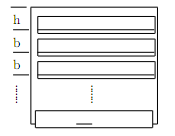
\includegraphics{./graphics/heightofpagebox.jpg}
\end{figure}
\end{comment}

\subsection{Dead cycles.} An execution of the OTR without shipping any material is called a \emph{dead cycle}. Dead cycles, have their uses and we will explain this a bit later on. However, long iterations that just return \textit{dead cycles} is an indication of an error somewhere. \tex counts the number of dead cycles in a counter named |\deadcycles| and stops the run if |\deadcycles >= \maxdeadcycles|.  In the \textit{plain} format |\maxdeadcycles| is set as 25 and in \latex as \the\deadcycles. |\maxdeadcycles = 100| is \the\maxdeadcycles. Each time |\shipout| is invoked, it resets |\deadcycles| to zero.

\begin{dispListing}
If the file is not included, reset \deadcycles, so that a long list of non-included
files does not generate an `Output loop' error.
115 \deadcycles\z@
116 \@nameuse{cp@#1}%
117 \fi
118 \let\@auxout\@mainaux}
\end{dispListing}


\subsection{\tex's Page Number.} The page number can come from any source. Salomon provides an example where the \textsc{OTR} typesets a page number from a |\count| variable. This is typeset centered below the printed area.

%\newpage
%
%Test
%\makeatletter
%
%\let\ltxxoutput\output
%\let\ltxlabel\label@name
%\output={{\let\label@name\@gobble
%  \shipout\vbox{
%  \box255\smallskip
%  \centerline{\thepage}}}
%}
%
%\vfill \penalty-10000
%
%\global\let\output\ltxxoutput
%\let\label@name\ltxlabel
%
%
%\makeatother


Notice that the output macro, just passes the contents of the box to |\shipout|. This is not actually a very good method, but is shown here to illustrate a point.

Note the |\tenrm| in the preceding example. It
is necessary because of the asynchronous nature of
the \otr. When the \otr is invoked, \tex can be
anywhere on the next page. Specifically, it could
be inside a group where a different font is used.
Without the |\tenrm|, that font (the current font)
would be used in the otr.
In the plain format, the |\count0| variable
serves as the page number, and the following two
macros are especially useful.




\subsection{The \texttt{\textbackslash vsplit} operation.} 

Supposed you have inserted the material required to go on a page on a big |\vbox|, but the material is a bit extra that what is required to fill a page exactly. You would need an operation to split the box in two. The |vsplit| operation does that. It is important to the understanding of OTR operations to have an intimate knowledge of |\vsplit|. Its syntax is: 

\begin{quote}
|\vsplit|\meta{box number} to \meta{dim}
\end{quote}

The result of the operation is a box. Most often it appears in an assignment such as: 

\begin{quote}
|\setbox1=\vsplit0 to2.6in| 
\end{quote}

This sets |\box1| to a
height of 2.6in, moves material from the top of
|\box0| to |\box1|, and keeps the remainder in |\box0|.

\begin{macro}{\loremlines}
It is important to remember that most of \tex's commands work with \latex as well. In Example~\ref{ex:loremlines}, we define a box to hold |lipsum| text in a two column layout. We want to define a macro that can split the box in as many lines as we require. 
\end{macro}

\begin{texexample}{Splitting a vbox}{ex:loremlines}
\newbox\one
\newbox\two
\long\gdef\loremlines#1#2{%
   \setbox\one=\vbox {#2}
   \setbox\two=\vsplit\one to #1\baselineskip
   \unvbox\two
   \gdef\boxone{#2}
}
\begin{multicols}{2}
\small
\loremlines{16}{\onepar}
\end{multicols}
\boxone

\setbox\one=\vbox{100}
\the\ht\one \\
\the\baselineskip
\the\splittopskip

\end{texexample}


\tex assumes that the new |\box1| may have to
be shipped out as part of the page. It therefore
places a glue similar to $h$ at the top of |\box1|.
This glue is called \docAuxCommand{splittopskip} and has a plain
format value of 10pt [348].

One important thing to note is that a box can only be split \textit{between} lines of text. 
If we split a box to another size, |\box1| will come out underfull.

Here is an \otr which splits the page, ships
out the top part and returns the rest to the MVL
(actually, to the recent contributions):

\begin{teXXX}
\output={\setbox0=\vsplit255 to1in
\shipout\box0 \unvbox255}
\end{teXXX}






\section{Communicating with the OTR: Marks}


The user can pass information to the output routine through \textit{marks}. Marks have the syntax

\begin{teX}
\mark{mark text}
\end{teX}

which is put in a mark item on the current vertical list. The mark text is subject to expansion
as in \cs{edef}.
If the mark is given in horizontal mode it migrates to the surrounding vertical lists like an
insertion item (see page Text By Topic 77); however, if this is not the external vertical list, the output routine
will not find the mark.

Marks are the main mechanism through which the output routine can obtain information
about the contents of the currently broken-off page, in particular its top and bottom. TEX sets
three variables:

{\obeylines
\cs{botmark} the last mark occurring on the current page;
\cs{firstmark} the first mark occurring on the current page;
\cs{topmark} the last mark of the previous page, that is, the value of \cs{botmark} on the previous
page.
}



If no marks have occurred yet, all three are empty; if no marks occured on the current page, all three variables are equal to the \cs{botmark} of the previous page. 

Marks can be used to get a section heading into the headline or footline of the page.

\begin{quote}
\begin{verbatim}
\def\section#1{ ... \mark{#1} ... }
\def\rightheadline{\hbox to \hsize
    {\headlinefont \botmark\hfil\pagenumber}}
\def\leftheadline{\hbox to \hsize
   {\headlinefont \pagenumber\hfil\firstmark}}
\end{verbatim}
\end{quote}

This places the title of the first section that starts on a left page in the left
headline, and the title of the last section that starts on the right page in
the right headline. Placing the headlines on the page is the job of the output
routine; see below.

It is important that no page breaks can occur in between the mark and the
box that places the title:

\emphasis{mark,nobreak}
\begin{teXXX}
\def\section#1{ ...
   \penalty\beforesectionpenalty
   \mark{#1}
   \hbox{ ... #1 ...}
   \nobreak
   \vskip\aftersectionskip
   \noindent}
\end{teXXX}

%%%%%%%%%%%% macro to put TeX references in right margin %%%%%%%% 
\newdimen\theight 
\def \TeXref#1{% 
             \vadjust{\setbox0=\hbox{\sevenrm\quad\quad\TeX book: #1}% 
             \theight=\ht0 
             \advance\theight by \dp0    \advance\theight by \lineskip 
             \kern -\theight \vbox to \theight{\rightline{\rlap{\box0}}% 
             \vss}% 
             }}% 
%%%%%%%%%%%%%%%%%%%%%%%%%%%%%%%%%%%%%%%%%%%%%%%%%%%%%%%%%%%%%%%%%%%%%%%%% 
 
However, useful these marks, sometimes an output routine (such as those found in \latexe needs to know why it was invoked. Knuth discusses in the \TeXref{396}  another method
that involves the value of the |\outputpenalty|. 
By testing for this value, it is possible to see what penalty occurred at a breakpoint;
any penalty of −10000, −10001, −10002, or less, forces the output routine to
act, hence different penalty values can be used to pass different messages. (When
the output routine puts material back on the list of contributions, it need not restore
the penalty at the breakpoint.) If output has been forced by a highly negative value
of |\outputpenalty|, the output routine can use |\vbox{\unvcopy255}| to discover how
full the page-so-far actually is. Underfull and overfull boxes are not reported when
|\box255| is packaged for use by the output routine, so there’s no harm in ejecting a
page prematurely if you want to pass a signal. (Set |\holdinginserts| positive to pass
a signal when the contents of |\box255| will be sent back through the page builder again,
if any insertions are present.)

Knuth also suggested another method that he called the \emph{dirtiest trick of all} that uses the depth 
of |\box255|. 

\section{Insertions}
Insertions are considered one of  the most  complex  topics in \tex. Many users master  topics  such 
as tokens,  file  I/O, macros,  and  even  OTRS  before they dare  tackle  insertions.  The  reason  is  that 
insertions  are  complex,  and  The \texbook, while 
covering all the relevant material, is somewhat cryptic regarding  insertions, and  lacks  simple examples. 
The  main  discussion  of  insertions takes  place  on 
[115-1251.  where \tex' s  registers  are also discussed. 
Examples  of  insertions are  shown, mostly  without 
explanations,  on  [363-364,  423-424].  A lot of what is described here is based on an article in TUGboat by David Salomon\footnote{\protect\url{http://www.tug.org/TUGboat/Articles/tb11-4/tb30salomon.pdf}}

Many users understand the idea of floats. Certain material to be typeset needs to be held in a buffer and inserted at different points on a page, for example a a figure that does not fit on a page it has to be inserted at the top of the next page. An \textit{insertion} is just a piece of a document that is generated at a certain point but appears at another point. Common examples are figures, footnotes and endnotes. Quoting Knuth:

\begin{quote}
  This  algorithm  is  admittedly  complicated, 
but  no  simpler  mechanism  seems  to  do  nearly 
as  much.
\end{quote}

\section{\protect\textbackslash shipout}

The primitive control sequence \docAuxCommand{shipout} is \tex's end game. It's syntax is quite simple:

\begin{quote}
|\shipout<box>|
\end{quote}

From TeXbook, Chapter 23: Output Routines, page 254:

\begin{quotation}
TeX’s primitive command |\shipout<box>| is what actually causes output. It sends the contents of the box to the dvi file, which is TeX’s main output file; after TeX has finished, the dvi file will contain a compact device-independent encoding of instructions that specify exactly what should be printed. When a box is shipped out, TeX displays the values of |\count0| through |\count9| on your terminal, as explained in Chapter 15; these ten counters are also recorded in the dvi file, where they can be used to identify the page. All of the |\openout, \closeout|, and |\write| commands that appear inside of the box are performed in their natural order as that box is being shipped out. Since a |\write| command expands macros, as explained in Chapter 21, TeX’s scanning mechanism might detect syntax errors while a |\shipout| is in progress. If  |\tracingoutput| is nonzero at the time of a \cs{shipout}, the contents of the box being shipped are written into your log file in symbolic form. You can say \cs{shipout} anywhere, not only in an output routine.
\end{quotation}


We can say:

\emphasize{shipout,vbox}
\begin{teXXX}
\shipout\vbox{%
  \hrule
  \medskip
  \lipsum[1-5]
  \medskip
  
  This is a Test for shipout
  
  \hrule
}
\end{teXXX}

\shipout\vbox{%
  \hrule
  \medskip
  \lipsum[1-5]
  \medskip
  \centering
  \textbf{Sample: }{This is a Test for shipout}
  \hrule
}

Since the output box handled by \tex still holds material the page is shown in the previous page. There is no page numbers or headers and it just shows he lorem-ipsum text and a primitive caption at the bottom. I have written the example to show the difference between the logical and actual pages. TeX does not care how the page will look, it will assemble it put headers, page numbers and pass it on to shipout. Shipout will then insert it to the dvi file, which will hold all teh instructions to print a real page.

We can modify the example to add our head and foot. 

\begin{texcode}{Shipout}{ex:ship2}
This will print by the normal routine

\long\gdef\boxit#1#2{\hbox{\vrule \vbox{\hrule\kern#2pt\hbox{%
\kern#2pt\vbox{#1}\kern#2pt}\kern#2pt\hrule}\vrule}}

\makeatletter
\shipout\vbox {%
  \vskip\topsep\relax
  \vskip\headsep
   \@thehead
   \vskip30pt
    \boxit{
      \lipsum[1-5]
      }{2}
   \vskip30pt
   \@thefoot   
}
\makeatother 
\end{texcode}

\latexe's output routine takes care of all the page geometry, the details to set up the headers and footers, but most importantly intercepts teh contents of the output box measure it, cuts it inserts the inserts such as footnotes and figures, margin notes, separates the text in two columns if necessary and so on. 

\long\gdef\boxit#1#2{\hbox{\vrule \vbox{\hrule\kern#2pt\hbox{%
\kern#2pt\vbox{#1}\kern#2pt}\kern#2pt\hrule}\vrule}}
\makeatletter
\shipout\vbox {%
  \vskip\topsep\relax
  \vskip\headsep
   \@thehead
   \vskip30pt
    \boxit{
      \lipsum[1-5]
      }{2}
   \vskip30pt
   \@thefoot   
}
\makeatother 



An output routine will prepare the virtual page and pass it onto a 

Here is an OTR for a \textit{framed} page. It surrounds the
page with double rules on all sides, and centers the
page number below the double box. Note that the
page shipped out is wider and taller than \cs{box255}.
The value of \cs{hsize} in this case is, therefore, not
the width of the final page shipped out, but the
width of the text lines in \cs{box255}.

Macro \cs{frameit} typesets text and surrounds it
with 4 rules (see [Ex. 21.3]). Parameter \#2 is the
space between the rules and the text. \#1 is a box
containing the text.

\emphasis{output,shipout}
\begin{texcode}{Example of simple output routine}{ex:output1}
\def\frameit#1#2{%
 \vbox{\hrule
  \hbox{%
    \vrule \kern#2pt
      \vbox{\kern#2pt #1
         \kern#2pt}%
      \kern#2pt\vrule}
\hrule}}

\output={
   \shipout\vbox{
   \boxit{\frameit{\box255}9}
      \medskip
      \centerline{Test Framed Page}}
  \advancepageno}
\end{texcode}

 

So far we did not care if the height of the page is right or not. In production code the shipout holds
a box, which has been produced by \tex. Any material we add to it, must not affect the dimensions of the box.
If we do and is too big the drivers will probably clip it.


Plain TeX has an output routine that takes care of  simple things like page numbering and insertions
using \cs{footnote} and \cs{topinsert}. 


So far we have examined the \tex OTR in detail. I hope it has given you enough understanding, not only to write your own output routine, but also to now be ready to study the \latex output routine, which is much more complicated. We have so far seen that  when \tex 
is typesetting pages of continuous text, it will gather material until it can find a least-cost page break intended to
make the gathered material fit the \cs{pagegoal} size. The
gathered material will then be placed into |\box255| and
the output routine stored in the token register \cs{output}
will be processed in a group of its own. 

Usually it will
arrange the gathered material in some way, add headers,
footlines and page numbers, and ship the gathered results out in typeset form with the \cs{shipout} command.
At the time of the \cs{shipout} command all \cs{open} and
\cs{write} commands stored in the box shipped out are expanded and written out. This is what makes it possible to have page labels corresponding to the actual page
numbers at the time of shipout: the corresponding info
is written to the |.aux| file at that time.
The output routine may decide to place material
back on the main vertical list instead of shipping it out. Its ob is to check if it can have a break, if it can it will ship the page out. If it cannot it will palce the material back on the main vertical list. 

\section{\LaTeX\  output routines}


\LaTeX\ output routine is described in \texttt{ltoutput.dtx}. You should also have a look at \texttt{ltfloat.dtx}. The algorithm is revisited i \latex3 and Frank Mittelbach, published a paper
\footnote{\protect\url{http://www.latex-project.org/papers/xo-pfloat.pdf}} in which he explains some of the problems facing the team, when dealing with the output routine.


Information on the output routine is rather scarce. Best source is a series of  articles in the TUGBoat by David Salomon.

\href{http://www.tug.org/TUGboat/Articles/tb11-1/tb27salomon.pdf}{Output Routines: Examples and Techniques. Part I: Introduction and Examples.}

\href{http://www.tug.org/TUGboat/Articles/tb11-2/tb28salomon.pdf}{Output Routines: Examples and Techniques. Part II: OTR Techniques}

\href{http://www.tug.org/TUGboat/Articles/tb11-4/tb30salomon.pdf}{Output Routines: Examples and Techniques. 
Part III: Insertions}

\href{http://www.tug.org/TUGboat/Articles/tb15-1/tb42salomon-output.pdf}{Output routines: Examples and techniques Part IV: Horizontal techniques}


David Kastrup's article \href{http://www.tug.org/TUGboat/Articles/tb24-3/kastrup.pdf}{Output Routine Requirements for Advanced Typesetting Tasks} (Proceedings of EuroTEX 2003) otlined some of the difficult areas and specifications for generic routines

The standard blocks are well described above and most tasks could be accomplished 
by rather working from
standard building blocks like \textit{insertion lists}, \textit{here points},
default mechanisms for \textit{margin notes} and so on.


%\section{Calling the output routine}
%
%The output routine is called either by TeX's normal page-breaking
%mechanism, or by a macro putting a penalty < or = -10000 in the output
%list. In the latter case, the penalty indicates why the output
%routine was called, using the following code.
%penalty reason
%
%\begin{longtable}{ll}
%\toprule
%penalty &reason\\
%\midrule
%-10000  &\ pagebreak\\
%~       &\ newpage\\
%-10001  &clearpage (\ penalty -10000 \ vbox{}| \ penalty -10001)|\\
%-10002  &float insertion, called from horizontal mode\\
%-10003 &float insertion, called from vertical mode.\\
%-10004 &float insertion.\\
%\bottomrule
%\end{longtable}
%\medskip
%
%Note: A |float| or |marginpar| puts the following sequence in the output
%list: 
%
%\begin{enumerate}
%\item a penalty of -10004,
%
%\item a null |\vbox|
%
%\item a penalty of -10002 or -10003.
%\end{enumerate}
%
%This solves two special problems:
%
%\begin{enumerate}
%\item If the float comes right after a |\newpage| or |\clearpage|,
%then the first penalty is ignored, but the second one
%invokes the output routine.
%
%\item If there is a split footnote on the page, the second 'page'
%puts out the rest of the footnote
%\end{enumerate}
%
%\latex first defines some helper routines and increase the \cs{maxdeadcycles}. The helper macros are for
%manipulating lisst.
%
%\begin{teX}
% \maxdeadcycles = 100
% \let\@elt\relax
% \def\@next#1#2#3#4{\ifx#2\@empty #4\else
%   \expandafter\@xnext #2\@@#1#2#3\fi}
%   \@next \CS \LIST {NONEMPTY}{EMPTY} == %% NOTE: ASSUME
%\@elt = \relax
% BEGIN assume that \LIST == \@elt \B1 ... \@elt \Bn
% if n = 0
% then EMPTY
% else 
%   \CS :=L \B1
%   \LIST :=G \@elt \B2 ... \@elt \Bn
%   NONEMPTY
% fi
%END
%\end{teX}
%
%
%\begin{teX}
%11 \def\@xnext \@elt #1#2\@@#3#4{\def#3{#1}\gdef#4{#2}}
%
%12 \def\@testfalse{\global\let\if@test\iffalse}
%13 \def\@testtrue {\global\let\if@test\iftrue}
%14 \@testfalse}
%   }
%
%15 \def\@bitor#1#2{\@testfalse {\let\@elt\@xbitor
%16   \@tempcnta #1\relax #2}}
%
%17 \def\@xbitor #1{\@tempcntb \count#1
%18    \ifnum \@tempcnta =\z@
%19    \else
%20      \divide\@tempcntb\@tempcnta
%21    \ifodd\@tempcntb \@testtrue\fi
%22   \fi}
%\end{teX}
%
%
%\subsection{Float boxes and lists.} 
%A \textit{float list} consisting of the 
%floats in boxes |\boxa ... \boxN| has
%the form:
%
%|\@elt \boxa ... \@elt \boxN|
%where |\boxI| is defined by
%
%|\newinsert\boxI|
%
%Normally, |\@elt| is |\let| to |\relax|. A test can be performed on the
%entire 
%oat list by locally |\def|'ing |\@elt| appropriately and
%executing the list.
%This is a lot more efficient than looping through the list.
%\LaTeX\ defines float boxes as |bx@A| to |bx@R| to make them available for 
%inserts. These will be used later to define the lists that hold these boxes. 
%
%\latex now defines the float boxes. Each one is defined as an \cmd{\newinsert.}
%
%\begin{teXXX}
%\newinsert\bx@A
%...
%\newinsert\bx@I
%\newinsert\bx@J
%\newinsert\bx@K
%\newinsert\bx@L
%\newinsert\bx@M
%\newinsert\bx@N
%\newinsert\bx@O
%\newinsert\bx@P
%\newinsert\bx@Q
%\newinsert\bx@R
%\end{teXXX}
%
%
%
%Once these boxes are defined they are inserted in the |@freelist|. At this point all the other lists are defined.
%
%\emphasis{@freelist,@toplist,@botlist,@midlist,@currlist}
%\begin{teXXX}
%41 \gdef\@freelist{\@elt\bx@A\@elt\bx@B\@elt\bx@C\@elt\bx@D
%         \@elt\bx@E
%42                 \@elt\bx@F\@elt\bx@G\@elt\bx@H\@elt\bx@I\@elt\bx@J
%43                 \@elt\bx@K\@elt\bx@L\@elt\bx@M\@elt\bx@N
%44                 \@elt\bx@O\@elt\bx@P\@elt\bx@Q\@elt\bx@R}
%\end{teXXX}
%
%\startlineat{45}
%All the lists are defined initially to be empty.
%\begin{teXXX}
%45 \gdef\@toplist{}
%46 \gdef\@botlist{}
%47 \gdef\@midlist{}
%48 \gdef\@currlist{}
%49 \gdef\@deferlist{}
%50 \gdef\@dbltoplist{}
%51 \gdef\@dbldeferlist{}
%\end{teXXX}
%
%
%The lists are similar to those defined in \texttt{plain}.
%
%\begin{description}
%\item[\cs{@freelist}] : List of empty boxes for placing new 
%floats.
%\item[\string\@toplist] : List of 
%floats to go at top of current column.
%\item[\string\@midlist] : List of 
%floats in middle of current column.
%\item[\string\@botlist] : List of 
%floats to go at bottom of current column.
%\item[\string\@deferlist] : List of 
%floats to go after current column.
%\item[\string\@dbltoplist] : List of double-col. 
%floats to go at top of current
%page.
%\item[\string\@dbldeferlist] : List of double-column 
%floats to go on subsequent
%pages.
%
%\end{description}
%
%\begin{multicols}{2}
%Check was prudent when defining the newinsert boxes in order to reserve space and memory. The package \docpkg{morefloats} can be used to add more floats to this list. This should have definitely been included here in a revision.
%
%\subsection{Defining Layout parameters} All the page layout parameters are defined next. 
%
%\begin{teXXX}
%52 \newdimen\topmargin
%53 \newdimen\oddsidemargin
%54 \newdimen\evensidemargin
%55 \let\@themargin=\oddsidemargin
%56 \newdimen\headheight
%57 \newdimen\headsep
%58 \newdimen\footskip
%59 \newdimen\textheight
%60 \newdimen\textwidth
%61 \newdimen\columnwidth
%62 \newdimen\columnsep
%63 \newdimen\columnseprule
%64 \newdimen\marginparwidth
%65 \newdimen\marginparsep
%66 \newdimen\marginparpush
%\end{teXXX}
%
%Remember  that TeX knows little about a page. The problem is that TEX has no idea how
%wide and tall the paper is. All it knows is the
%left and top offsets, and the dimensions of the
%printed area (|\hsize| and |\vsize|). All these dimensions need to be calculated and adjustments made within the \otr.
%
%A document normally  starts by specifying:
%
%\begin{teXXX}
%\newdimen\paperheight
%\newdimen\paperwidth
%\paperheight=..in \paperwidth=..in
%\end{teXXX}
%
%
%\end{multicols}
%
%
%\subsection*{The AtBeginDvi}
%A box register is used  to put stuff that must appear before anything else
%in the |.dvi| file.
%
%The stuff in the box should not add any typeset material to the page when it
%is unboxed.
%
%\emphasis{AtBeginDvi,@begindvibox}
%
%\begin{teXXX}
%67 \newbox\@begindvibox
%68 \def \AtBeginDvi #1{%
%69 \global \setbox \@begindvibox
%70 \vbox{\unvbox \@begindvibox #1}%
%71 }
%\end{teXXX}
%
%\begin{teXXX}
%72 \newdimen\@maxdepth
%73 \@maxdepth = \maxdepth
%\end{teXXX}
%
%
%Some new registers for paperheight and paperwidth are defined:
%
%\begin{teXXX}
%74 \newdimen\paperheight
%75 \newdimen\paperwidth
%76 \newif \if@insert
%These should definitely be global:
%77 \newif \if@fcolmade
%78 \newif \if@specialpage \@specialpagefalse
%These should be global but are not always set globally in other les.
%79 \newif \if@firstcolumn \@firstcolumntrue
%80 \newif \if@twocolumn \@twocolumnfalse
%Not sure about these: two questions. Should things which must apply to a whole
%doument be local or global (they probably should be `preamble only' commands)?
%Are these three such things?
%81 \newif \if@twoside \@twosidefalse
%82 \newif \if@reversemargin \@reversemarginfalse
%83 \newif \if@mparswitch \@mparswitchfalse
%This counter has been imported from `multicol'.
%84 \newcount \col@number
%85 \col@number \@ne
%\end{teXXX}
%
%and a lot of other internal registers
%
%\begin{teX}
%86 \newcount\@topnum
%87 \newdimen\@toproom
%88 \newcount\@dbltopnum
%89 \newdimen\@dbltoproom
%90 \newcount\@botnum
%91 \newdimen\@botroom
%92 \newcount\@colnum
%93 \newdimen\@textmin
%94 \newdimen\@fpmin
%95 \newdimen\@colht
%96 \newdimen\@colroom
%97 \newdimen\@pageht
%98 \newdimen\@pagedp
%99 \newdimen\@mparbottom \@mparbottom\z@
%100 \newcount\@currtype
%101 \newbox\@outputbox
%102 \newbox\@leftcolumn
%103 \newbox\@holdpg
%104 \def\@thehead{\@oddhead} % initialization
%105 \def\@thefoot{\@oddfoot}
%\end{teX}
%
%
%\subsection{\texttt{\textbackslash clearpage}}
%
%\begin{macro}{\clearpage}
%The clearpage macro is a bit complicated, as it needs to avoid a complete empty page after a |\twocolumn[..]|. This prevents the text from the argument
%vanishing into a  float box, never to be seen again. We hope that it does not
%produce wrong formatting in other cases.
%\end{macro}
%
%\begin{teXXX}
%106 \def\clearpage{%
%107   \ifvmode
%108   \ifnum \@dbltopnum =\m@ne
%109     \ifdim \pagetotal <\topskip
%110       \hbox{}%
%111     \fi
%112   \fi
%113  \fi
%114 \newpage
%115 \write\m@ne{}%
%116 \vbox{}%
%117 \penalty -\@Mi
%118 }
%\end{teXXX}
%
%\subsection{The \texttt{\textbackslash clearpagedoublepage} macro} 
%
%\begin{macro}{cleardoublepage}
%This checks for odd and even pages by using the
%page counter |c@page|.  It also provides switches of twoside printing. 
%
%\numberlineat{119}
%\begin{teXXX}
%\def\cleardoublepage{%
%   \clearpage
%   \if@twoside 
%     \ifodd\c@page
%     \else
%       \hbox{}
%       \newpage
%       \if@twocolumn\hbox{}\newpage
%       \fi
%     \fi
%  \fi}
%\end{teXXX}
%\end{macro}
%
%Note the |\newpage| is defined a bit further on. This is a fairly simple definition, since most of the code that follows only gets a bit complicated with the twocolumn option. It sets the dimensions and the booleans to those appropriate for the |onecolumn| option. An important note we back to \tex's |\hsize|. Both the linewidth as well as the columnwidth are set to this.
%
%\begin{teXXX}
%123 \def\onecolumn{%
%124   \clearpage
%125   \global\columnwidth\textwidth
%126   \global\hsize\columnwidth
%127   \global\linewidth\columnwidth
%128   \global\@twocolumnfalse
%129   \col@number \@ne
%130   \@floatplacement
%     }
%\end{teXXX}
%
%\subsection{\string newpage.} 
%
%The |\newpage| macro is programmed defensively. The two checks at the beginning ensure that an item label or run-in section title
%immediately before a |\newpage| get printed on the correct page, the one before
%the page break.
%All three tests are largely to make error processing more robust; that is why
%they all reset the 
%flags explicitly, even when it would appear that this would be
%done by a |\leavevmode|.
%
%\begin{teXXX}
%131 \def \newpage {%
%132  \if@noskipsec
%133    \ifx \@nodocument\relax
%134      \leavevmode
%135      \global \@noskipsecfalse
%136    \fi
%137 \fi
%138 \if@inlabel
%139   \leavevmode
%140   \global \@inlabelfalse
%141 \fi
%142 \if@nobreak \@nobreakfalse \everypar{}\fi
%143 \par
%144 \vfil
%145 \penalty -\@M}
%\end{teXXX}
%
%An empty cols is defined. There is a note here, that an invisible rule might have been a better idea.
%
%\begin{teXXX}
%146 \def \@emptycol {\vbox{}\penalty -\@M}
%\end{teXXX}
%
%\subsection{The \string twocolumn macro.} This is the longest definition so far. We will leave it for a while and then come back. There are several bug fixes to the two-column stuff here. Firstly, like the onecolumn the page parameters are set to the correct parameters.
%
%
%\begin{teXXX}
%147 \def \twocolumn {%
%148 \clearpage
%149 \global\columnwidth\textwidth
%150 \global\advance\columnwidth-\columnsep
%151 \global\divide\columnwidth\tw@
%152 \global\hsize\columnwidth
%153 \global\linewidth\columnwidth
%154 \global\@twocolumntrue
%155 \global\@firstcolumntrue
%156 \col@number \tw@
%\end{teXXX}
%
%
%
%\section{The output macro}
%
%The setting of the \cs{output} is quite short but it belies its complexity.
%After having checked verious parameters it redirects to |@specialoutput|. This is the heart of the routines. Notice that \latex just fills in the token list of \tex's |output| routine, it does not attempt to redefine it or save it. 
%Should some hooks be defined here, life might have been made easier, however, what one can do is to first save the \latex output routine and then redefine the output as one may wish. Return to it can happen after it. If you take this approach, you should be careful of packages that redefine output, such as |multicol| and |longtable|. An approach such as this is taken by \citeauthor{revtex} in the \pkgname{revtex} class.\footcite[][This is a document class of the American Physical Society. It enables submission to any of the APS journals. Its distribution point is \protect\url{http://publish.aps.org/revtex4/}]{revtex}
%
%\emphasis{ifnum,fi,else,ifdimen,@specialoutput}
%\begin{teX}
%204 \output {%
%205 \let \par \@@par
%206 \ifnum \outputpenalty<-\@M
%207    \@specialoutput
%208 \else
%209    \@makecol
%210    \@opcol
%211    \@startcolumn
%212    \@whilesw \if@fcolmade \fi
%213      {%
%218      \@opcol\@startcolumn}%
%219 \fi
%220 \ifnum \outputpenalty>-\@Miv
%221 \ifdim \@colroom<1.5\baselineskip
%222 \ifdim \@colroom<\textheight
%223 \@latex@warning@no@line {Text page \thepage\space
%224 contains only floats}%
%225 \@emptycol
%226 % \if@twocolumn
%227 % \if@firstcolumn
%228 % \else
%229 % \@emptycol
%230 % \fi
%231 % \fi
%232 \else
%  233 \global \vsize \@colroom
%234 \fi
%235 \else
%236   \global \vsize \@colroom
%237 \fi
%238 \else
%239   \global \vsize \maxdimen
%240 \fi
%241 }
%\end{teX}
%
%
%
%\begin{teXXX}
%244 \gdef\@specialoutput{%
%245   \ifnum \outputpenalty>-\@Mii
%246     \@doclearpage
%247   \else
%248     \ifnum \outputpenalty<-\@Miii
%249         \ifnum \outputpenalty<-\@MM \deadcycles \z@ \fi
%250                 \global \setbox\@holdpg \vbox {\unvbox\@cclv}%
%251         \else
%252         \global \setbox\@holdpg \vbox{%
%253                 \unvbox\@holdpg
%254                 \unvbox\@cclv
%We must now remove the box added by the 
%oat mechanism and the \topskip
%glue therefore added above it by TEX.
%255                \setbox\@tempboxa \lastbox
%256                \unskip
%257 }%
%These two are needed as separate dimensions only by \@addmarginpar; for other
%purposes we put the whole size into \@pageht (see below).
%258                \@pagedp \dp\@holdpg
%259                \@pageht \ht\@holdpg
%260                \unvbox \@holdpg
%
%261                \@next\@currbox\@currlist{%
%262                \ifnum \count\@currbox>\z@
%Putting the whole size into \@pageht (see above).
%263                  \advance \@pageht \@pagedp
%264                  \ifvoid\footins \else
%265                    \advance \@pageht \ht\footins
%266                    \advance \@pageht \skip\footins
%267                    \advance \@pageht \dp\footins
%268                \fi
%\end{teXXX}
%
%
%
%\subsection{The \string @doclearpage macro.} This is an emergency action. It dumps everything: footnotes first and then floats. 
%
%
%\section*{The Kludgeins}
%
%The kludgeins are simply inserts that fool \tex in enlarging a page by a small amount, normally used to allow one or two lines of text to go in the same page.
%
%The two kludgeins mentioned in the kernel are are \cs{enlargethisspace} and its star version.\footnote{The Oxford English Dictionary (2nd ed., 1989) kludge entry cites one source for this word's earliest recorded usage, definition, and etymology: Jackson W. Granholm's 1962 "How to Design a Kludge" article, which appeared in the American computer magazine Datamation
%kludge  Also kluge. [J. W. Granholm's jocular invention: see first quot.; cf. also bodge v., fudge v.]
%
%'An ill-assorted collection of poorly-matching parts, forming a distressing whole' (Granholm); esp. in Computing, a machine, system, or program that has been improvised or 'bodged' together; a hastily improvised and poorly thought-out solution to a fault or 'bug'.
%
%The word 'kludge' is...derived from the same root as the German Kluge..., originally meaning 'smart' or 'witty'.... 'Kludge' eventually came to mean 'not so smart' or 'pretty ridiculous'.}
%
%
%
%\begin{teXX}
%\gdef \enlargethispage{%
%1198 \@ifstar
%1199 {%
%1203   \@enlargepage{\hbox{\kern\p@}}}%
%1204 {%
%1208   \@enlargepage\@empty}%
%1209 }
%\end{teXX}
%
%Adds |<dim>| to the height of the current column only. On the printed page the
%bottom of this column is extended downwards by exactly |<dim>| without having
%any effect on the placement of the footer; this may result in an overprinting.
%\cs{enlargethispage}.
%
%Similar to |\enlargethispage| but it tries to squeeze the column to be printed
%in as small a space as possible, ie it uses any shrinkability in the column. If the
%column was not explicitly broken (e.g. with |\pagebreak|) this may result in an
%overfull box message but except for this it will come out as expected (if you know
%what to expect).
%The star form of this command is dedicated to Leslie Lamport, the other we
%need for ourselves (FMi, CAR).
%These commands may well have unwanted if used soon before a\ldots
%
% 




\section{Packages}

OTR routines are notoriously difficult to debug and define. Some of the available packages at CTAN
can make the programming job easier.

The \pkg{everypage} package by Sergio Callegari provides hooks into the \latex\ internal commands to
to do actions on every page or on the current page. Specifically, actions  are performed \emph{before} the page is shipped, so they can be used to put watermarks \emph{in the background} of a page, or to
set the page layout. 

The package provides two hooks:

\emphasis{AddEverypageHook,AddThisPageHook}
\begin{teXXX}
  \AddEverypageHook{Test}
  \AddThisPageHook
\end{teXXX}

The package reminds in some sense
\pkgname{bobhook} by Karsten Tinnefeld, but it differs in the way in
 which the hooks are implemented, as detailed in the following.
 In some sense it may also be related to the package
 \pkgname{everyshi} by Martin Schroeder, but again the implementation
 is different.

 
 This program adds two \LaTeX\ hooks that get run when document
 pages are finalized and output to the |.dvi| or |.pdf|
 file. Specifically, one hook gets executed on every page, while the
 other is executed for the current page. Hook actions are are performed
 \emph{before} the page is output on the medium, and this is
 important to be able to play with the page layout or to put things
 \emph{behind} the page contents (e.g., watermarks such as an image,
 framing, the ``DRAFT'' word, and the like).
 
 The package reminds in some sense \pkg{bobhook} by Karsten
 Tinnefeld, but it differs in the way in which the hooks are
 implemented:
 


 \begin{enumerate}
 \item there is no formatting inherent in the hooks. If one wants to
   put some watermark on a page, it is his own duty to put in the
   hook the code to place the watermark in the right position. Also
   note that the hooks code should \emph{eat up no space} in the
   page.  Again, if the hooks are meant to place some material on the
   page, it is the duty of the hook programmer to put code in the
   hooks to pretend that the material has zero width and zero height.
   The implementation is \emph{lighter} than the \Lpack{bobhook} one,
   and possibly more flexible, since one is not limited by any
   pre-coded formatting for the hooks. On the other hand it is
   possibly more difficult to use. Nonetheless, it is easy to think
   of other packages relying on \Lpack{everypage} to deliver more
   user-friendly and \emph{task specific} interfaces. Already there
   are a couple of them: the package \Lpack{flippdf} produces
   mirrored pages in a PDF document and \Lpack{draftwatermark}
   watermarks document pages.
 \item similarly to \Lpack{bobhook} and \Lpack{watermark}, the
   package relies on the manipolatoin of the internal \LaTeX\ macro
   |\@begindvi| to do the job. However, the redefinition of
   |\@begindvi| is here postponed as much as possible, striving to
   avoid interference with other packages using |\AtBeginDvi| or
   anyway manipulating |\@begindvi|. Specifically \Lpack{everypage}
   makes no special assumption on the initial code that |\@begindvi|
   might contain.
 \end{enumerate}



Also in some sense \pkgname{everypage} can be related to package
 \pkgname{everyshi} by Martin Schr\"oeder \cite{everyshi}, but it differs radically from
 it in the implementation. In fact,\pkgname{everypage} operates by
 manipulation of the |\@begindvi| macro, rather than at the
 lower level |\shipout| macro.

\section{hooking at shipout}

\begin{docCmd} {EveryShipout} {}
\begin{docCmd} {AtNextShipout} {}
This package provides the hooks \cs{EveryShipout} and 
  \cs{AtNextShipout} whose arguments are executed after the output 
  routine has constructed \cs{box255}, and before \cs{shipout} is 
  called.
\end{docCmd}
\end{docCmd}

An example application for this package would be a package for
 adding text to the bottom of each page.
 The  \pkgname{prelim2e} package adopts this method \citep{prelim2e}.\footcite{prelim2e}

The solution  uses is based on code developed in  |quire.tex| by
 Marcel R.~van der Goot.\footcite{quire}  

The \pkgname{prelim2e}  intercepts and modifies the |\box255|. 

\begin{teX}
44 \newcommand{\@Prelim@EveryShipout}{%
45 \bgroup
% First we save the dimensions of \box255: height, width and depth; and calculate
% the total height of \box255.
46 \dimen\z@=\wd\@cclv
47 \dimen\@ne=\ht\@cclv
48 \dimen\tw@=\dp\@cclv
49 \dimen\thr@@=\dimen1
50 \advance\dimen\thr@@ by \dimen\tw@
% Then we set \box255: A \vbox to the total height of \box255. In this a \hbox to
% the width of \box255 is included, in which \box255 is set.
51 \global\setbox\@cclv\vbox to \dimen\thr@@{%
52 \hb@xt@\dimen\z@{%
53 \box\@cclv%
54 \hss
55 }%
\end{teX}
To this we append the text produced by |\PrelimText|. It is put in a |\vbox to 0pt|
in which a |\hbox| to the width of |\box255| is included, in which |\PrelimText| is set.
We have to reset |\protect| because it is set to |\noexpand| by the output routine.

\begin{teXXX}
56 \vbox to \z@{%
57   \hb@xt@\dimen\z@{%
58     \let\protect\relax
59     \hfill\PrelimText\hfill
60   }%
61   \vss
62 }%
63   \vss
64 }%
\end{teXXX}

Finally we set the dimensions of |\box255| to the values they had before |\@Prelim@EveryShipout|.

\begin{teX}
65 \wd\@cclv=\dimen\z@
66 \ht\@cclv=\dimen\@ne
67 \dp\@cclv=\dimen\tw@
68 \egroup
69}
\end{teX}

Once the command is defined, it is hooked into the system via |\EveryShipout| when it is in draft mode. 

\begin{teX}
70 \if@prelim@draft
71 \EveryShipout{\@Prelim@EveryShipout}
72 \fi
\end{teX}

\section{How to place a background image}

One can use \tikzname to place a background image or some text on a page

First we define some utility macros:


\begin{teX}
\def\bg@contents{Draft}
\def\bg@color{red!45}
\def\bg@angle{60}
\def\bg@opacity{.5}
\def\bg@scale{15}
\def\bg@position{current page.center}
\def\bg@anchor{}
\def\bg@hshift{0}
\def\bg@vshift{0}
\end{teX}

A new command is then developed to describe the background material

\begin{teXXX}
\newcommand\bg@material{%
   \begin{tikzpicture}[remember picture,overlay]
   \node [rotate=\bg@angle,scale=\bg@scale,opacity=\bg@opacity,%
   xshift=\bg@hshift,yshift=\bg@vshift,color=\bg@color]
   at (\bg@position) [\bg@anchor] {\bg@contents};
  \end{tikzpicture}}%
\end{teXXX}


Once the background material has been defined we can place it on the page by simply calling:

\begin{teX}
\newcommand\BgThispage{\AddThispageHook{\bg@material}}
\end{teX}


The \pkgname{background}\footcite{background} package by \citeauthor has capitalized on two good packages the \tikzname and the \pkgname{everypage}.
\footcite{everypage} As most of modern
\tex programming works with |pdf| files, package developers prefer to use \tikzname methods for hooking directly into the pdf and thus avoid a trip into the output routine. If it is required then it hooks via the dvi or shipout commands.\footnote{These packages are loaded automatically by the \pkgname{phd-pkgmanager}.}



\vfill

\message{(total: \the\pagetotal
depth: \the\pagedepth
shrink: \the\pageshrink
stretch: \the\pagestretch}



 







































\cxset{fashion image=fashion-03.jpg,
       palette rouge}
       
\chapter{ltoutput.dtx}

\label{kernel:ltoutput}

\section{Introduction}

 In Chapter \ref{ch:OTR}, we described the mechanics of output routines both
 as found in Plain \tex and in \LaTeXe. This is
 a longer treatise of the subject and includes commentary on the
 actual listing as found in \LaTeXe. The Output Routine (OR) or (OTR) as is sometimes denoted in the literature, is the procedure
by which \LaTeXe\ assembles the material that makes a page by combining
text and floats, adding any other inserts such as footnotes, headers and
footers and then ships out the page to produce a |.dvi| or with some \tex engines to
be translated straight into |.pdf| output. It is a very complex process
as it has to keep a lot of different material in different lists and boxes.

The output routine as defined in the kernel covers a lot of functionality.

\begin{enumerate}
\item Defines page geometry parameters.
\item Positions floats.
\item Adds headers and footers.
\item Adds hooks.
\end{enumerate}


 \section{Floats}

The interesting and complicated part of the OR is its algorithm for handling floats.  The floating environments are defined by the standard classes. For example the |book| class defines both
the figure as well as the table environments. It is instructive to start the discussion of the algorithm from this point. 

The class defines the default float placement specifier using 
|\fps@figure| and then goes on to define the figure environment with the help of \refCom{@float} and \refCom{end@float}, which are defined in the generic \docFile{float.dtx} in the kernel.


\begin{teX}
\def\ftype@figure{1}
\def\ext@figure{lof}
\def\fnum@figure{\figurename\nobreakspace\thefigure}
\newenvironment{figure}
               {\@float{figure}}
               {\end@float}
\newenvironment{figure*}
               {\@dblfloat{figure}}
               {\end@dblfloat}
\end{teX}


A float specifier is made of two parts the float type, which is a power of two--e.g., figures in the case of the book class are type 1 and tables type 2 and the \textit{placement specification} describing where the float can be placed.  The type is defined in powers of two due to the way the specifiers are represented using a binary representation internally.

\ExplSyntaxOn
\int_to_bin:n {50}\\
\int_from_bin:n {110010}
\ExplSyntaxOff

\begin{figure}[h]
\centering
\begin{tabular}{rl}
{\fboxsep2pt   \fbox{1} \fbox{1} \fbox{0} \fbox{0} \fbox{1} \fbox{0}} &= 50\\
{\fboxsep2pt \fbox{1} \fbox{0} \fbox{1} \fbox{0} \fbox{0} \fbox{1} \fbox{0}} &= 82
\end{tabular}

\caption{Binary representation of float specifiers. Top is for figure with [t] option and the bottom is for table with the [t] option.}
\end{figure}

So a new float will need to be shifted in powers of two. The kernel defines routines to check
for various combinations. This has simplified the programming although it may not be easy to
follow. The float specifier is encoded as follows, where bit 0 is the least
 significant bit. 

\begin{table}[h]
\begin{tabular}{ll}
\toprule
  Bit    & Meaning\\
\midrule
   0     & 1 if the float may go where it appears in the text.\\
   1     & 1 if the float may go on the top of a page.\\
   2     & 1 if the float may go on the bottom of a page.\\
   3     & 1 if the float may go on a float page.\\
   4     & 1 unless the \textit{placement} includes a !\\
   5     & 1 if a type 1 float\\
   6     & 1 if a type 2 float
          etc.\\
\bottomrule
\end{tabular}
\end{table}

If a number is odd  denotes  a here placement specification [h] and if it is negative a marginpar. 
Since TeX's number limit of $ 2^{31}-1$ and the first 5 bits are taken by the float identifiers there remain 26 available float types for the adventurous. \url{http://tex.stackexchange.com/questions/32359/what-is-the-exact-purpose-of-ftypetype}.

We have seen so far how a float is defined in the standard classes and what type of parameters are coded. Once \LaTeXe\  sees the environment it will execute the macro |\@float| which is defined in the |float.dtx|. 

Once in |\@float| the bits are set as well as the relevant penalties. The penalties are distinct in order to signal to the output routines the type of float.

One needs to remember that the floats are placed based on constraints and page sizing parameters.


\section{Page Layout Parameters}

\begin{longtable}[l]{p{4.5cm}p{8.5cm}}
   |\topmargin|      & Extra space added to top of page.\\
   |\@twoside|       & boolean.  T if two-sided printing\\
   |\oddsidemargin|  & IF @twoside = T
                       THEN extra space added to left of odd-numbered
                            pages.
                       ELSE extra space added to left of all pages.\\
   |\evensidemargin| & IF @twoside = T
                       THEN extra space added to left of even-numbered
                            pages.\\
   |\headheight|     & height of head\\
   |\headsep|        & separation between head and text\\
   |\footskip|         & distance separation between baseline of last
                     line of text and baseline of foot.
                     Note difference between |\footSKIP| and |\headSEP|.\\

   |\textheight|     & height of text on page, excluding head and foot\\

   |\textwidth|      & width of printing on page\\
   |\columnsep|      & IF @twocolumn = T
                       THEN width of space between columns\\

   |\columnseprule|  & IF @twocolumn = T
                       THEN width of rule between columns (0 if none).\\

   |\columnwidth|    & IF @twocolumn = T
                       THEN |(\textwidth - \columnsep)|/2
                       ELSE |\textwidth|
                     It is set by the |\twocolumn| and
                     |\onecolumn| commands.\\

   |\@textbottom|    & Command executed at bottom of vbox holding text of
                     page (including figures).  The |\raggedbottom|
                     command almost |\let|'s this to |\vfil| (actually sets
                     it to |\vskip \z@| plus.0001fil).
                     Should have depth 0pt.\\

   |\@texttop|       & Command executed at top of vbox holding text of
                     page (including figures).  Used by letter style;
                     can also be used to produce centered pages.
                     Let to |\relax| by |\raggedbottom| and |\flushbottom|.\\
\end{longtable}


Page layout must initialize |\@colht| and |\@colroom| to |\textheight|.

\section{Page Style Parameters}

\begin{longtable}{p{3.5cm}p{7.5cm}}
   |\floatsep|       & Space left between floats.\\
   |\textfloatsep|   & Space between last top float or first bottom float
                     and the text.\\
   |\topfigrule|     & Command to place rule (or whatever) between floats
                     at top of page and text.  Executed in inner
                     vertical mode right before the |\textfloatsep| skip
                     separating the floats from the text.  Must occupy
                     zero vertical space.  (See |\footnoterule|.)\\
   |\botfigrule|     & Same as |\topfigrule|, but put after the
                     |\textfloatsep| skip separating text from the
                     floats at bottom of page.\\
   |\intextsep|      & Space left on top and bottom of an in-text float.\\
   |\dblfloatsep|    & Space between double-column floats.\\
   |\dbltextfloatsep| & Space between top double-column floats
                      and text.\\
   |\dblfigrule|     & Similar to |\topfigrule|, but for double-column
                     floats.\\
   |\@fptop|         & Glue to go at top of float column -- must be 0pt +
                     stretch\\
   |\@fpsep|         & Glue to go between floats in a float column.\\
   |\@fpbot|         & Glue to go at bottom of float column
                       -- must be 0pt +
                     stretch\\
   |\@dblfptop|, |\@dblfpsep|, |\@dblfpbot|
                   & Analogous for double-column float page in
                     two-column format.\\

   |@twocolumn|      & Boolean.  T if two columns per page globally.\\


   |\@oddhead|        & IF @twoside = T
                           THEN macro to generate head of odd-numbered
                                pages.
                           ELSE macro to generate head of all pages.\\
   |\@evenhead|      & IF @twoside = T
                           THEN macro to generate head of even-numbered
                                pages.\\
   |\@oddfoot|        & IF @twoside = T
                           THEN macro to generate foot of odd-numbered
                                pages.
                           ELSE macro to generate foot of all pages.\\
   |\@evenfoot|       & IF @twoside = T
                           THEN macro to generate foot of even-numbered
                                pages.\\
   |@specialpage|     & boolean.  T if current page is to have a special
                               format.\\
  |\@specialstyle|   & If its value is  foo then
                     IF @specialpage = T
                       THEN the command |\ps@foo| is executed to
                            temporarily reset the page style parameters
                            before composing the current page.
                            This command should execute only |\def|'s and
                            |\edef|'s, making only local definitions.\\
\end{longtable}



\section{Float placement parameters}

 The following parameters are set by the macro |\@floatplacement|.
 When |\@floatplacement| is called,
 |\@colht| is the height of the page or column being built.  I.e.:

         * For single-column page it equals |\textheight|.\\
         * For double-column page it equals |\textheight| - height
           of double-column floats on page.

 Note that some are set globally and some locally:

\begin{description}

  \item[\cs{@topnum}] = G Maximum number of floats allowed on the top of a
                  column.
  \item [\cs{@toproom}] :=G Maximum amount of top of column devoted to floats--
                  excluding |\textfloatsep| separation below the floats
                  and |\floatsep| separation between them.  For
                  two-column output, should be computed as a function
                  of |\@colht|.
\end{description}


\begin{longtable}{p{4.5cm}p{5.5cm}}
    |\@botnum|, |\@botroom|
                & Analogous to above.\\
    |\@colnum|  & G Maximum number of floats allowed in a column,
                  including in-text floats.\\
    |\@textmin| & L Minimum amount of text (excluding footnotes) that
                  must appear on a text page.
                  It is used locally in processing double
                  floats.\\
    |\@fpmin|   & L Minimum height of floats in a float column.\\
\end{longtable}


 The macro \cs{@dblfloatplacement} sets the following parameters.

\begin{tabular}{p{3.5cm}p{6cm}}
    |\@dbltopnum|  &G Maximum number of double-column floats allowed at
                     the top of a two-column page.\\
    |\@dbltoproom|  &G Maximum height of double-column floats allowed at
                     top of two-column page.\\
    |\@fpmin|      &L Minimum height of floats in a float column.\\
\end{tabular}

 It should also perform the following local assignments where necessary
 -- i.e., where the new value differs from the old one:

\begin{tabular}{p{3.5cm}p{6cm}}
     |\@fptop|    & L |\@dblfptop|\\
     |\@fpsep|      & L |\@dblfpsep|\\
     |\@fpbot|      &L |\@dblfpbot|\\
\end{tabular}


\section{Output Routine Variables}


\begin{tabular}{p{3.5cm}p{6cm}}
  |\@colht| & The total height of the current column.  In single column
            style, it equals |\textheight|.  In two-column style, it is
            |\textheight| minus the height of the double-column floats
            on the current page.  MUST BE INITIALIZED TO |\textheight|.\\

  |\@colroom| & The height available in the current column for text and
              footnotes.  It equals |\@colht| minus the height of all
              floats committed to the top and bottom of the current
              column.\\

  |\@textfloatsheight| & The total height of in-text floats on the
                       current page.\\

  |\footins| & Footnote insertion number.\\

  |\@maxdepth| & Saved value of TeX's |\maxdepth|.  Must be set
               when any routine sets |\maxdepth|.\\
\end{tabular}



\section{Calling the output routine}

 The output routine is called either by TeX's normal page-breaking
 mechanism, or by a macro putting a penalty \(\le -10000\) in the output
 list.  In the latter case, the penalty indicates why the output
 routine was called, using the following code.

\begin{table}[ht]
\centering
\begin{tabular}{lp{6cm}}
\toprule
   Penalty   & Reason\\
\midrule
   -10000    & \cs{pagebreak}\\
             & \cs{newpage}\\
   -10001    & \cs{clearpage} (\cs{penalty} -10000 \cs{vbox}|{}| \cs{penalty} -10001)\\
   -10002    & float insertion, called from horizontal mode\\
   -10003    & float insertion, called from vertical mode.\\
   -10004    & float insertion.\\
\bottomrule
\end{tabular}
\caption{Penalties when calling the output routine.}
\end{table}
Note that a float or marginpar puts the following sequence in the output
list:
\begin{enumerate} 
  \item a penalty of -10004,
  \item a null |\vbox|
  \item a penalty of -10002 or -10003.
\end{enumerate}

This solves two special problems:

\begin{enumerate}
  \item If the float comes right after a \cs{newpage} or \cs{clearpage},
        then the first penalty is ignored, but the second one
       invokes the output routine.
 \item If there is a split footnote on the page, the second 'page'
       puts out the rest of the footnote.
\end{enumerate}
             

            
\section{Functions used in the output routine}

\begin{docCommand}{@outputpage}{}
 \cs{@outputpage} : Produces an output page with the contents of box
              |\@outputbox| as the text part.
              Also sets |\@colht| :=G |\textheight|.
              The page style is determined as follows:
              
              \begin{algorithm}[H]
               \Begin{
                \If{\cs{@thispagestyle} = true}{
                   use \cs{thispagestyle} style}{
                   use ordinary page style.}}
              \end{algorithm}
\end{docCommand}


\begin{docCommand}{@tryfcolumn}{}
\begin{description}
 \item[\cs{@tryfcolumn}\cs{FLIST}]  tries to form a float column composed of floats
         from |\FLIST| (if nonempty) with the following parameters see \autoref{tryfcolumn}:
 
           \begin{tabular}{p{3cm}l}
                |\@colht|  & height of box\\
                |\@fpmin| & minimum height of floats in the box\\
                |\@fpsep|  & interfloat space\\
                |\@fptop | & glue at top of box\\
                |\@fpbot | & glue at bottom of box.\\
          \end{tabular}


  If it succeeds, then it does the following:

         \begin{tabular}{p{3cm}l}
                 |\@outputbox| & L the composed float box.\\
                 |@fcolmade|   & G true\\
                 |\FLIST|          & G |\FLIST| - floats put in box\\
                 |\@freelist|     & G |\@freelist| + floats put in box\\
         \end{tabular}

              If it fails, then:

         \begin{tabular}{ll}
                |@fcolmade| & G false\\
        \end{tabular}
           NOTE: BIT MUST BE A SINGLE TOKEN!
\end{description}
\end{docCommand}




\begin{docCommand}{@makefcolumn}{}
 |\@makefcolumn \FLIST| is similar to |\@tryfcolumn| except that it
             fails to make a float column only if |\FLIST| is empty.
             Otherwise, it makes a float column containing at least
             the first box in |\FLIST|, disregarding |\@fpmin|.
\end{docCommand}

\begin{docCommand}{@startcolumn}{}

\begin{description}
\item[ \cs{@startcolumn} ]
       Calls |\@tryfcolumn\@deferlist|.  If |\@tryfcolumn| returns with
       (globally set) @fcolmade = false, then:

\item           Globally sets |\@toplist| and |\@botlist| to floats
                  from |\@deferlist| to go at top and bottom of column,
                  deleting them from |\@deferlist|.  It does
                  this using |\@colht| as the total height, the page
                  style parameters |\@floatsep| and |\@textfloatsep|, and
                  the float placement parameters |\@topnum|, |\@toproom|,
                  |\@botnum|, |\@botroom|, |\@colnum| and |\textfraction|.

\item          Globally sets |\@colroom| to |\@colht| minus the height
                  of the added floats.
\end{description}
\end{docCommand}




\begin{docCommand}{@startdblcolumn }{}

      Calls |\@tryfcolumn\@dbldeferlist{8}|.  If |\@tryfcolumn| returns
      with (globally set) @fcolmade = false, then:

               * Globally sets |\@dbltoplist| to floats from
                 |\@dbldeferlist| to go at top and bottom of column,
                 deleting them from |\@dbldeferlist|.
                 It does this using |\textheight| as the
                 total height, and the parameters |\@dblfloatsep|, etc.

               * Globally sets |\@colht| to |\textheight| minus the height
                 of the added floats.

\end{docCommand}

\begin{docCommand}{@combinefloats}{}
 \cs{@combinefloats} Combines the text from box
          \cs{@outputbox} with the floats from \cs{@toplist} and \cs{@botlist},
          putting the new box in \cs{@outputbox}.  It uses \cs{floatsep}
          and \cs{textfloatsep} for the appropriate separations.
          It puts the elements of \cs{TOPLIST} and \cs{BOTLIST} onto
          \cs{@freelist}, and makes those lists null.

\end{docCommand}

\begin{docCommand}{@makecol}{}
|\@makecol| Makes the contents of |\box255| plus the accumulated
              footnotes, plus the floats in |\@toplist| and |\@botlist|,
              into a single column of height |\@colht| (unless the page
              height has been locally changed), which it puts
              into box |\@outputbox|.  It puts boxes in |\@midlist| back
              onto |\@freelist| and restores |\maxdepth|.
\end{docCommand}



\begin{docCommand}{@opcol}{}
 \cs{@opcol} Outputs a column whose text is in box \cs{@outputbox}
\end{docCommand}
%
%\begin{algorithm}
% \cs{@opcol}==\Begin{%    
%\eIf{@twocolumn = false}{\cs{@outputpage}\\
%  \cs{@colht} :=G \cs{textheight}\\
%  \cs{@floatplacement}}{\eIf{@firstcolumn = true}{puts box \cs{@outputbox}
%      into \cs{@leftcolumn}\\
%      @firstcolumn :=G false.}{puts out the current two-column page\\
%      any possible two-column float pages,\\
%      determine \cs{@dbltoplist} for the next page.}}
%}
%\end{algorithm}



\section{User commands  that call  affect the output routine}

\begin{docCommand}{newpage}{}
 \begin{teX}
 \newpage == BEGIN \par\vfil\penalty -10000 END
 \end{teX}
\end{docCommand}

\begin{docCommand}{clearpage}{}
\begin{verbatim}
              == BEGIN \newpage
                     \write -1{}    % Part of hack to make sure no
                     \vbox{}        % \write's get lost.
                     \penalty -10001
               END
\end{verbatim}
\begin{verbatim}
 \cleardoublepage == BEGIN \clearpage
                           if @twoside = true and c@page is even
                             then \hbox{} \newpage fi
                     END

  
 \twocolumn[BOX] : starts a new page, changing to twocolumn setting
     and puts BOX in a parbox of width \textwidth across the top.
     Useful for full-width titles for double-column pages.
     SURPRISE: The stretch from \@dbltextfloatsep will be inserted
               between the BOX and the top of the two columns.
\end{verbatim}
\end{docCommand}


\section{Float-handling mechanisms}

 The float environment obtains an insertion number B from the
 |\@freelist| (see below for a description of list manipulation), puts
 the float into box B and sets |\count| B to a FLOAT SPECIFIER.  For
 a normal (not double-column) float, it then causes a page break
 in one of the following two ways:

   - In outer hmode: |\vadjust{\penalty -10002}|
   - In vmode :      |\penalty -10003.|

 For a double-column float, it puts B onto the |\@dbldeferlist|.


 The float specifier has two components:

    * A PLACEMENT SPECIFICATION, describing where the float may
      be placed.

    * A TYPE, which is a power of two--e.g., figures might be
      type 1 floats, tables type 2 floats, programs type 4 floats, etc.

 The float specifier is encoded as follows, where bit 0 is the least
 significant bit.
\medskip


\begin{tabular}{ll}
\toprule
  Bit    & Meaning\\
\midrule
   0     & 1 if the float may go where it appears in the text.\\
   1     & 1 if the float may go on the top of a page.\\
   2     & 1 if the float may go on the bottom of a page.\\
   3     & 1 if the float may go on a float page.\\
   4     & 1 unless the PLACEMENT incluses a !\\
   5     &  if a type 1 float\\
   6     & 1 if a type 2 float
          etc.\\
\bottomrule
\end{tabular}
\medskip

A negative float specifier is used to indicate a marginal note.



\section{Macros and data structures for processing floats}

  A \textit{float list} consisting of the floats in boxes |\boxa ... \boxN| has
  the form:

  \begin{verbatim}
         \@elt \boxa ... \@elt \boxN
  \end{verbatim}

  where  |\boxI| is defined by:

  \begin{verbatim}
         \newinsert\boxI
  \end{verbatim}

  Normally, |\@elt| is |\let| to |\relax|.  A test can be performed on the
  entire float list by locally |\def|'ing |\@elt| appropriately and
  executing the list.

  This is a lot more efficient than looping through the list.

  The following macros are used for manipulating float lists. Of interest here---and a bit
  difficult to follow is |\@next| see \ref{next}.

  \begin{verbatim}
  \@next \CS \LIST {NONEMPTY}{EMPTY} ==  %% NOTE: ASSUME \@elt = \relax
    BEGIN  assume that \LIST == \@elt \B1 ... \@elt \Bn
           if n = 0
             then  EMPTY
             else   \CS    := L \B1
                     \LIST  := G \@elt \B2 ... \@elt \Bn
                   NONEMPTY
           fi
    END
  \end{verbatim}



\begin{docCommand}{@bitor}{\Arg{num}\Arg{list}}
  \cs{@bitor}|\NUM\LIST|  Globally sets switch |@test| to the disjunction for
         all I of bit  log2 |\NUM| of the float specifiers of all the
         floats in |\LIST|.

         I.e., @test is set to true iff there is at least one
         float in |\LIST| having bit  log2 |\NUM|  of its float specifier
         equal to 1.
\end{docCommand}
\begin{verbatim}
%  Note: log2 [(\count I)/32] is the bit number corresponding to the
%  type of float I.  To see if there is any float in \LIST having
%  the same type as float I, you run \@bitor with
%
%    \NUM = [(\count I)/32] * 32.
%
% \@bitor\NUM\LIST ==
%   BEGIN
%      @test :=G false
%      { \@elt \CTR ==  if \NUM <> 0 then
%                          if \count\CTR / \NUM is odd
%                             then  @test := true       fi fi
%        \LIST
%      }
%   END
%
%
% \@cons\LIST\NUM : Globally sets \LIST := \LIST * \@elt \NUM
%
% \@cons\LIST\NUM ==
%   BEGIN {  \@elt == \relax
%            \LIST :=G \LIST \@elt \NUM
%         }

\end{verbatim}



\section{Box lists for float-placement algorithms}

The \pkg{fixltx2e} the now redundant package---as it was incorporated into the fixes
provided by |fixltx2e|--- modify the output routine to correct a problem with synchronizing floats in double column texts with those in single column \cite{fix2col,fixltx2e}. Here we will describe the normal behaviour.
Additional commentary on the changes is discussed later on.
 
\begin{tabular}{p{3cm}p{6cm}}
    |\@freelist|     & List of empty boxes for placing new floats.\\
    |\@toplist|      & List of floats to go at top of current column.\\
    |\@midlist|      & List of floats in middle of current column.\\
    |\@botlist|      & List of floats to go at bottom of current column.\\
    |\@deferlist|    & List of floats to go after current column.\\
    |\@dbltoplist|   & List of double-col. floats to go at top of current
                     page.\\
    |\@dbldeferlist| & List of double-column floats to go on subsequent
                     pages.\\
\end{tabular}

\begin{texexample}{Meaning toplist}{ex:toplist}
\makeatletter
\meaning\@freelist\\
\meaning\@toplist
\makeatother
\end{texexample}

\section{Float-Placement algorithms}


\begin{docCommand}{@addtobot}{}  Tries to put insert |\@currbox| on |\@botlist|.
                     Called only when:

                  * |\ht BOX < \@colroom|\\
                  * type of |\@currbox| not on |\@deferlist|\\
                  * |\@colnum > 0|\\
                  * @insert = false\\
\end{docCommand}



               If it succeeds, then:
\begin{trivlist}
                  \item  sets @insert true\\
                  \item  decrements |\@botroom| by |\ht| BOX\\
                  \item  decrements |\@botnum| and |\@colnum| by 1\\
                  \item decrements |\@colroom| by |\ht| BOX + either |\floatsep|
                    or |\textfloatsep|, as appropriate.\\
                 \item sets |\maxdepth| to 0pt\\
\end{trivlist}



\begin{docCommand}{@addtotoporbot}{}

 Tries to put insert |\@currbox| on |\@toplist| or
                    |\@botlist|.

                    Called only under same conditions as |\@addtobot|.

                    If it succeeds, then:
                       * sets @insert true
                       * decrements |\@toproom| or |\@botroom| by |\ht| BOX
                       * decrements |\@colnum| and either |\@topnum| or
                         |\@botnum| by 1
                       * decrements |\@colroom| by |\ht| BOX + |\floatsep|
                         or |\textfloatsep|, as appropriate.
\end{docCommand}

\begin{docCommand}{@addtocurcol}{}
  Tries to add |\@currbox| to current column, setting
                 @insert true if it succeeds, false otherwise.
                 It will add |\@currbox| to top only if bit 0 of
                |\count \@currbox| is 0, and to the bottom only if
                 bit 0 = 0 or an earlier float of the same type is
                 put on the bottom.

                 If the float is put in the text, then
                 |\penalty\interlinepenalty| is put
                 right after the float, before the following |\vskip|,
                 and 
                     
                         |\outputpenalty :=L 0.|
\end{docCommand}

\begin{docCommand}{@addtonextcol}{} Tries to add |\@currbox| to the next column, setting
                  @insert true if it succeeds, false otherwise.
\end{docCommand}

\begin{docCommand}{@addtodblcol}{} Tries to add |\@currbox| to the next double-column page,
                 adding it to |\@dbltoplist| if it succeeds and
                 |\@dbldeferlist| if it fails.
\end{docCommand}


%\begin{algorithm}
%  \cs{@addmarginpar} ==\\
%   \Begin{
%     \eIf{\cs{@currlist} nonempty}{
%        remove \cs{@marbox} from \cs{@currlist}\\
%        add \cs{@marbox} and \cs{@currbox} to \cs{@freelist}\\
%         NOTE: \cs{@currbox} = left box}{
%         LaTeX error: ?  \\
%     }
%     \cs{@tempcnta} := 1\\     %% 1 = right, -1 = left
%     \eIf{@twocolumn = true}{
%       then if @firstcolumn = true
%              then \cs{@tempcnta} := -1
%            fi}{
%            \eIf{@mparswitch = true}{
%               \If{count0 odd}{}{
%                   \cs{@tempcnta} := -1
%               }
%            }
%            \If{@reversemargin = true}{
%               \cs{@tempcnta} := -\cs{@tempcnta}
%            }
%     }
%
%     \If{\cs{@tempcnta} < 0}{\cs{box}\cs{@marbox} :=G \cs{box}\cs{@currbox}}
%     
%     \cs{@tempdima}   :=L maximum(\cs{@mparbottom} - \cs{@pageht}
%                                           + ht of \cs{@marbox}, 0)\\
%
%     \If{\cs{@tempdima} > 0}{LaTeX warning: 'marginpar moved'}
%
%     \cs{@mparbottom} :=G \cs{@pageht} + \cs{@tempdima} + depth of \@cs{marbox}
%                          + \cs{marginparpush}\\
%
%     \cs{@tempdima}   :=L \cs{@tempdima} - ht of \@cs{marbox}\\
%
%     \cs{box}\cs{@marbox} :=G \cs{box}\cs{@currbox}\\
%                                \cs{vbox}\{ \cs{vskip}\cs{@tempdima}\\
%                                        \cs{box}\cs{@marbox}\\
%                                       \}\\
%     height of \cs{@marbox} :=G depth of \cs{@marbox} :=G 0\\
%     \cs{kern} -\cs{@pagedp}\\
%     \cs{nointerlineskip}\\
%     
%     hbox\{\eIf{@tempcnta > 0}{hskip columnwidth\\
%                              hskip marginparsep}{
%                             hskip -marginparsep\\
%                             hskip -marginparwidth}
%             \cs{box}\cs{@marbox}\cs{hss}
%          \}\\
%     \cs{nobreak}\\
%     \cs{nointerlineskip}\\
%     \cs{hbox}\{\cs{vrule} height=0 width=0 depth=\cs{@pagedp}\}
%  }
%\end{algorithm}

 Floats and marginpars add a lot of dead cycles.

    \begin{teX}
\maxdeadcycles = 100
    \end{teX}

    \begin{teX}
\let\@elt\relax
    \end{teX}

\begin{docCommand}{@next}{}{}{}{}
    \begin{teX}
\def\@next#1#2#3#4{\ifx#2\@empty #4\else (*@\label{next}@*)
   \expandafter\@xnext #2\@@#1#2#3\fi}
    \end{teX}
\end{docCommand}

    \begin{teX}
\def\@xnext \@elt #1#2\@@#3#4{\def#3{#1}\gdef#4{#2}}
    \end{teX}


    \begin{teX}
\def\@testfalse{\global\let\if@test\iffalse}
\def\@testtrue {\global\let\if@test\iftrue}
\@testfalse
    \end{teX}
%
\footnotechanges{v1.1v}{1996/07/26}{remove \cs{global} before \cs{@test...}}
    \begin{teX}
\def\@bitor#1#2{\@testfalse {\let\@elt\@xbitor
   \@tempcnta #1\relax #2}}
    \end{teX}
%    RmS 91/11/22: Added test for |\count#1 = 0|.
%                  Suggested by Chris Rowley.
%
%
% \changes{v1.1v}{1996/07/26}{remove \cs{global} before \cs{@test...}}
    \begin{teX}
\def\@xbitor #1{\@tempcntb \count#1
   \ifnum \@tempcnta =\z@
   \else
     \divide\@tempcntb\@tempcnta
     \ifodd\@tempcntb \@testtrue\fi
   \fi}
    \end{teX}
%
\section{Definition of Float Boxes (inserts)}

All boxes are defined using \refCom{newinsert}.  A total of eighteen insertions are defined here
and later on inserted in the freelist (See line \ref{freelist}).
    \begin{teX}
\newinsert\bx@A \newinsert\bx@B \newinsert\bx@C
\newinsert\bx@D \newinsert\bx@E \newinsert\bx@F
\newinsert\bx@G \newinsert\bx@H \newinsert\bx@I
\newinsert\bx@J \newinsert\bx@K \newinsert\bx@L
\newinsert\bx@M \newinsert\bx@N \newinsert\bx@O
\newinsert\bx@P \newinsert\bx@Q \newinsert\bx@R
    \end{teX}

\tex allows 255 classes of insertions |\insert0| to |\insert254|. It is important to remember that
every insert is tied to other registers of the same number. For example, |\insert100| is connected
with |\count100|, |\dimen100|, |\skip100| and |\box100|. plain \tex provides an allocation function
for insertions as it does for registers. Appendix B includes the command:
\begin{quotation}
|\newinsert\footins|
\end{quotation} 
which defines |\footins| as the number for footnote insertions.

\latex2e adopts similar definitions (see Chapter \ref{kernel:ltplain}). In the latest versions
allocations are extended with |\extrafloats|.

The |\@freelist| is defined next. Notice that |\@elt| is included here to enable
the manipulation of the list later on.

    \begin{teX}
\gdef\@freelist{\@elt\bx@A\@elt\bx@B\@elt\bx@C\@elt\bx@D\@elt\bx@E (*@\label{freelist} @*)
               \@elt\bx@F\@elt\bx@G\@elt\bx@H\@elt\bx@I\@elt\bx@J
                \@elt\bx@K\@elt\bx@L\@elt\bx@M\@elt\bx@N
                \@elt\bx@O\@elt\bx@P\@elt\bx@Q\@elt\bx@R}
    \end{teX}

The rest of the lists are defined below and they are initialized as empty lists.

    \begin{teX}
\gdef\@toplist{}
\gdef\@botlist{}
\gdef\@midlist{}
\gdef\@currlist{}
\gdef\@deferlist{}
\gdef\@dbltoplist{}
\gdef\@dbldeferlist{}
    \end{teX}

\begin{texexample}{Current list}{ex:currentlist}
\makeatletter
\meaning\@currlist

\meaning \bx@A

\the\bx@A

\the\dimen252

\the\count252

\the\skip252


\makeatother
\end{texexample}

\section{Page layout parameters}

The page layout parameters (all taking values by the standard classes later on
are defined here. They are important in building up the page calculations.

    \begin{teX}
\newdimen\topmargin
\newdimen\oddsidemargin
\newdimen\evensidemargin
\let\@themargin=\oddsidemargin
\newdimen\headheight
\newdimen\headsep
\newdimen\footskip
\newdimen\textheight
\newdimen\textwidth
\newdimen\columnwidth
\newdimen\columnsep
\newdimen\columnseprule
\newdimen\marginparwidth
\newdimen\marginparsep
\newdimen\marginparpush
    \end{teX}


After these preliminary definitions are made a box is defined to hold material 
that is inserterted before the dvi file is produced. This is a general hook
and widely used by package authors.

\begin{docCommand}{AtBeginDvi}{\marg{contents}}{}

Uses a box register in which to put
stuff that must appear before anything else in the
|.dvi| file.

The stuff in the box should not add any typeset material to the
page when it is unboxed.
\end{docCommand}
    
    \begin{teX}
\newbox\@begindvibox
\def \AtBeginDvi #1{%
  \global \setbox \@begindvibox
    \vbox{\unvbox \@begindvibox #1}%
}                             
    \end{teX}

  
  \begin{docCommand}{@maxdepth}{}
    This is not the right place to set this; it needs to be set in a
    class/style file when |\maxdepth| is set.

    Also, many settings to |\maxdepth| should be to |\@maxdepth|,
    probably?     

    \begin{teX}  
\newdimen\@maxdepth
\@maxdepth = \maxdepth
    \end{teX}
  \end{docCommand}


 \begin{docCommand}{paperheight}{}{}
 \begin{docCommand}{paperwidth}{}{}
 Although earlier on, page parameters have been defined, we also need to define the paper height
and width.
    \begin{teX}
\newdimen\paperheight
\newdimen\paperwidth
    \end{teX}
 \end{docCommand}
 \end{docCommand}

The following nine switches have to be defined to keep track of various options.
 \begin{docCommand}{if@insert}{}
 \end{docCommand}
 \begin{docCommand}{if@fcolmade}{}
 \end{docCommand}
 \begin{docCommand}{if@specialpage}{}
  \end{docCommand}
 \begin{docCommand}{if@firstcolumn}{}
  \end{docCommand}
 \begin{docCommand}{if@twocolumn}{}
 \end{docCommand}
 \begin{docCommand}{if@twoside}{}
 \begin{docCommand}{if@reversemarginpar}{}
 \begin{docCommand}{if@mparswitch}{}
 \begin{docCommand}{col@number}{}
 \end{docCommand}
 
 
    Local switches first:
    \begin{teX}
\newif \if@insert
    \end{teX}
    These should definitely be global:
    \begin{teX}
\newif \if@fcolmade
\newif \if@specialpage \@specialpagefalse
    \end{teX}
    These should be global but are not always set globally in other
    files. 
    \begin{teX}
\newif \if@firstcolumn \@firstcolumntrue
\newif \if@twocolumn   \@twocolumnfalse
    \end{teX}
    Not sure about these: two questions.
    Should things which must apply to a whole doument be local or
    global (they probably should be `preamble only' commands)?
    Are these three such things?
    \begin{teX}
\newif \if@twoside     \@twosidefalse
\newif \if@reversemargin \@reversemarginfalse
\newif \if@mparswitch  \@mparswitchfalse
    \end{teX}
    This counter has been imported from `multicol'.
    \begin{teX}
\newcount \col@number
\col@number \@ne
    \end{teX}
 
 \end{docCommand}
 \end{docCommand}
 \end{docCommand}


\section{Internal registers}

    \begin{teX}
\newcount\@topnum
\newdimen\@toproom
\newcount\@dbltopnum
\newdimen\@dbltoproom
\newcount\@botnum
\newdimen\@botroom
\newcount\@colnum
\newdimen\@textmin
\newdimen\@fpmin
\newdimen\@colht
\newdimen\@colroom
\newdimen\@pageht
\newdimen\@pagedp
\newdimen\@mparbottom \@mparbottom\z@
\newcount\@currtype
\newbox\@outputbox
\newbox\@leftcolumn
\newbox\@holdpg
    \end{teX}

The page headers and page footers are initialized to their odd values, this makes sense
as a document always starts at an odd number.
    \begin{teX}
\def\@thehead{\@oddhead} % 
\def\@thefoot{\@oddfoot}
    \end{teX}


  \begin{docCommand}{clearpage}{}
 The tests at the beginning are an experimental attempt to avoid a
 completely empty page after a |\twocolumn[...]|.  This prevents the
 text from the argument vanishing into a float box, never to be seen
 again.  We hope that it does not produce wrong formatting in other
 cases.
    \begin{teX}
\def\clearpage{%
  \ifvmode
    \ifnum \@dbltopnum =\m@ne
      \ifdim \pagetotal <\topskip
        \hbox{}%
      \fi
    \fi
  \fi
  \newpage
  \write\m@ne{}%
  \vbox{}%
  \penalty -\@Mi
}
    \end{teX}
 \end{docCommand}

  \begin{docCommand}{cleardoublepage}{}
  
    \begin{teX}
\def\cleardoublepage{\clearpage\if@twoside \ifodd\c@page\else
    \hbox{}\newpage\if@twocolumn\hbox{}\newpage\fi\fi\fi}
    \end{teX}
 \end{docCommand}

  \begin{docCommand}{onecolumn}{}
    \begin{teX}
\def\onecolumn{%
  \clearpage
  \global\columnwidth\textwidth
  \global\hsize\columnwidth
  \global\linewidth\columnwidth
  \global\@twocolumnfalse
  \col@number \@ne
  \@floatplacement}
    \end{teX}
 \end{docCommand}

  \begin{docCommand}{newpage}{}
    The two checks at the beginning ensure that an item label or
    run-in section title immediately before a |\newpage| get printed
    on the correct page, the one before the page break.

    All three tests are largely to make error processing more robust;
    that is why they all reset the flags explicitly, even when it
    would appear that this would be done by a |\leavevmode|. 
    \begin{teX}
\def \newpage {%
  \if@noskipsec 
    \ifx \@nodocument\relax
      \leavevmode
      \global \@noskipsecfalse 
    \fi
  \fi
  \if@inlabel
    \leavevmode
    \global \@inlabelfalse 
  \fi
  \if@nobreak \@nobreakfalse \everypar{}\fi
  \par
  \vfil
  \penalty -\@M}
    \end{teX}
  \end{docCommand}
  
  \begin{docCommand}{@emptycol}{}
    It may be better to use an invisible rule rather than an empty
    box here.  
    \begin{teX}
\def \@emptycol {\vbox{}\penalty -\@M}
    \end{teX}
  \end{docCommand}

  \begin{docCommand}{twocolumn}{}
  \begin{docCommand}{@topnewpage}{}
    There are several bug fixes to the two-column stuff here.
    \begin{teX}
\def \twocolumn {%
  \clearpage
  \global\columnwidth\textwidth
  \global\advance\columnwidth-\columnsep
  \global\divide\columnwidth\tw@
  \global\hsize\columnwidth
  \global\linewidth\columnwidth
  \global\@twocolumntrue
  \global\@firstcolumntrue
  \col@number \tw@
    \end{teX}
    There is no reason to put a |\@dblfloatplacement| here since
    |\@topnewpage| ignores these settings.
    The |\@floatplacement| is needed in case this comes after some
    changes.

    \begin{teX}
  \@ifnextchar [\@topnewpage\@floatplacement
}
    \end{teX}
    
    Note that here, getting a box from the freelist can assume
    success since this comes just after a |\clearpage|.
    \begin{teX}
\long\def \@topnewpage [#1]{%
  \@nodocument
  \@next\@currbox\@freelist{}{}%
  \global \setbox\@currbox
    \color@vbox 
      \normalcolor
      \vbox {%
        \hsize\textwidth
        \@parboxrestore
        \col@number \@ne
        #1%
        \vskip -\dbltextfloatsep
             }%
    \color@endbox
    \end{teX}
    Added size test and warning message; perhaps we should use
    an error message.

    \begin{teX}
  \ifdim \ht\@currbox>\textheight
    \ht\@currbox \textheight
  \fi
    \end{teX}

    This next line is not essential but it is more robust to make this
    value non-zero, in case of weird errors.

    This next bit is what is needed from |\@addtodblcol|, plus some
    extra checks for error trapping.
    \begin{teX}
  \global \count\@currbox \tw@
  \@tempdima -\ht\@currbox
  \advance \@tempdima -\dbltextfloatsep
  \global \advance \@colht \@tempdima
  \ifx \@dbltoplist \@empty
  \else
    \@latexerr{Float(s) lost}\@ehb
    \let \@dbltoplist \@empty
  \fi
  \@cons \@dbltoplist \@currbox
    \end{teX}
    This setting of |\@dbltopnum| is used only to change the
    typesetting in\\ |\@combinedblfloats|.
    \begin{teX}
  \global \@dbltopnum \m@ne
%<*trace>
    \tr@ce{dbltopnum set to -1 (= \the \@dbltopnum) (topnewpage)}%
%</trace>
    \end{teX}

    At points such as this we need to check that there is still a
    minimal amount of room left on the page; this uses an arbitrary
    small value at present; but note that this value is larger than
    that used when checking that page is too full of normal floats.
   
    If there is little room left we just force a page-break, OK?
    This involves producing two empty columns.  The second empty
    column may be produced by |\output|, in which case an extra,
    misleading, warning will be generated, OK?  (This happens only
    when there is too little room left on the page for any float.)
    Otherwise (ie if the size is such that it is allowed as a normal
    float) the extra |\@emptycol| will be invoked in the second
    column by the conditional code guarded by the |\if@firstcolumn|
    test.
    
    I now think that the cut-off point here should be |3\baselineskip|,
    but we make it a bit less so that 3 lines of text will be
    allowed, OK?

    Since this happens only when there is nothing on the page but the
    `top-box', the empty box should not cause any problem other than
    some overfull box messages, which is not entirely misleading.

    Here we need two page-ends since both columns need to be empty.

    \begin{teX}
  \ifdim \@colht<2.5\baselineskip
    \@latex@warning@no@line {Optional argument of \noexpand\twocolumn
                too tall on page \thepage}%
    \@emptycol
    \if@firstcolumn
    \else
      \@emptycol
    \fi
  \else
    \global \vsize \@colht
    \global \@colroom \@colht
    \@floatplacement
  \fi
}
    \end{teX}
  \end{docCommand}
  \end{docCommand}

\section{The \textbackslash output routine}

We now arrive at the interesting part. The |\output| is a token register that holds instructions
as to how the page is to be typeset. This is called automatically by \tex. Think of it as the
main function.

  \begin{docCommand}{output}{}
    This needs some small adjustments.  We cannot
    guarantee that the float mechanism will interact correctly with
    this stuff, but that mechanism does not always work properly
    with footnotes already.
    
    The reset of |\par| to the output routine.
    This avoids problems when the output routine is
    called within a list where |\par| may be a no-op.


    \begin{teX}
\output {%
  \let \par \@@par
  \ifnum \outputpenalty<-\@M
    \@specialoutput
  \else
    \@makecol
    \@opcol
    \@startcolumn
    \@whilesw \if@fcolmade \fi
      {\@opcol\@startcolumn}%
  \fi
  \ifnum \outputpenalty>-\@Miv
    \ifdim \@colroom<1.5\baselineskip
      \ifdim \@colroom<\textheight  
        \@latex@warning@no@line {Text page \thepage\space
                               contains only floats}%
        \@emptycol
      \else
        \global \vsize \@colroom
      \fi
    \else
      \global \vsize \@colroom
    \fi
  \else
    \global \vsize \maxdimen
  \fi
}
    \end{teX}
\end{docCommand}

\begin{docCommand}{@specialoutput}{}
 \end{docCommand}
    \begin{teX}
\gdef\@specialoutput{%
   \ifnum \outputpenalty>-\@Mii
     \@doclearpage
   \else
     \ifnum \outputpenalty<-\@Miii
       \ifnum \outputpenalty<-\@MM \deadcycles \z@ \fi
       \global \setbox\@holdpg \vbox {\unvbox\@cclv}%
     \else
    \end{teX}
%
%    Note that |\boxmaxdepth| should not be set here since we wish to
%    record the natural depth of the holdpg box.
%    
%    This is changed so as to not lose anything, such as writes
%    and marks, which may get into box 255 and should be returned to
%    the list.  This should only happen when the first penalty in the
%    mechanism is discarded and therefore |\@holdpg| should always be
%    void in this case.  This can happen because a penalty is
%    discarded whenever there is no box on the list.
%
%    It was just: |\setbox\@tempboxa \box \@cclv|.
%    
%    The last box which is removed is the box put there by the
%    double-penalty mechanism.  The |\unskip| then removes the
%    |\topskip| which is put there since the box is the first on the
%    page.
    \begin{teX}
       \global \setbox\@holdpg \vbox{%
                      \unvbox\@holdpg
                      \unvbox\@cclv
    \end{teX}
%    We must now remove the box added by the float mechanism and the
%    |\topskip| glue therefore added above it by \TeX.
    \begin{teX}
                      \setbox\@tempboxa \lastbox
                      \unskip
                                     }%
    \end{teX}
%    These two are needed as separate dimensions only by
%    |\@addmarginpar|; for other purposes we put the whole size into
%    |\@pageht| (see below).
    \begin{teX}
       \@pagedp \dp\@holdpg
       \@pageht \ht\@holdpg
       \unvbox \@holdpg
       \@next\@currbox\@currlist{%
         \ifnum \count\@currbox>\z@
    \end{teX}
%    Putting the whole size into |\@pageht| (see above).
    \begin{teX}
           \advance \@pageht \@pagedp
           \ifvoid\footins \else
             \advance \@pageht \ht\footins
             \advance \@pageht \skip\footins
             \advance \@pageht \dp\footins
           \fi
           \ifvbox \@kludgeins
    \end{teX}
%    We want to make the adjustment due to this insert only if the
%    non-star form is used.  The *-form will probably not work with
%    floats, but maybe it still could make some adjustment here even
%    so?
    \begin{teX}
             \ifdim \wd\@kludgeins=\z@
               \advance \@pageht \ht\@kludgeins
             \fi
           \fi
    \end{teX}
%    This version puts the inserts back just before the additional
%    material; it could be moved earlier, before unboxing the
%    page-so-far.  Neither is guaranteed not to put things on the wrong
%    page.  This version is similar to the original version.
    \begin{teX}
           \@reinserts
           \@addtocurcol
         \else
           \@reinserts
           \@addmarginpar
         \fi
         }\@latexbug
    \end{teX}
%    A 2e change: use |\addpenalty| instead of |\penalty| here.  Some 
%    penalty is needed to create a potential break-point immediately
%    after the reinserts (or the marginal).  Otherwise there can be no
%    possibility to break here and this can cause the reinserts or the
%    marginal to appear on the next page (which is often incorrect).
%    However, if the nobreak flag is true, a |\nobreak| must be
%    correct.
    \begin{teX}
       \ifnum \outputpenalty<\z@
         \if@nobreak
           \nobreak
         \else
           \addpenalty \interlinepenalty
         \fi
       \fi
     \fi
   \fi
}
    \end{teX}
 


  \begin{docCommand}{@doclearpage}{}
    This is a very much an emergency action, just dumping everything:
    footnotes first then floats.  A more sophisticated version is
    needed; but even more urgent is a bug-free version (see, for
    example, pr/3528).

    Also, it puts any left-over non-boxes (writes, specials, etc.) back
    after any float pages created: this is a very bad bug since,
    for example, a kludge insert will be in quite the wrong place
    and, worse, be irremovable and uncancelable.
    
    \begin{teX}
\def \@doclearpage {%
     \ifvoid\footins
    \end{teX}
%    We empty any left over kludge insert box here; this is a temporary fix.
%    It should perhaps be applied to one page of cleared floats, but
%    who cares?  The whole of this stuff needs completely redoing for
%    many such reasons.
    \begin{teX}
       \ifvbox\@kludgeins
         {\setbox \@tempboxa \box \@kludgeins}%
       \fi 
       \setbox\@tempboxa\vsplit\@cclv to\z@ \unvbox\@tempboxa
       \setbox\@tempboxa\box\@cclv
       \xdef\@deferlist{\@toplist\@botlist\@deferlist}%
       \global \let \@toplist \@empty
       \global \let \@botlist \@empty
       \global \@colroom \@colht
       \ifx \@currlist\@empty
       \else
          \@latexerr{Float(s) lost}\@ehb
          \global \let \@currlist \@empty
       \fi
       \@makefcolumn\@deferlist
       \@whilesw\if@fcolmade \fi{\@opcol\@makefcolumn\@deferlist}%
       \if@twocolumn
         \if@firstcolumn
           \xdef\@dbldeferlist{\@dbltoplist\@dbldeferlist}%
           \global \let \@dbltoplist \@empty
           \global \@colht \textheight
           \begingroup
              \@dblfloatplacement
              \@makefcolumn\@dbldeferlist
              \@whilesw\if@fcolmade \fi{\@outputpage
                                        \@makefcolumn\@dbldeferlist}%
           \endgroup
         \else
           \vbox{}\clearpage
         \fi
       \fi
     \else
       \setbox\@cclv\vbox{\box\@cclv\vfil}%
       \@makecol\@opcol
       \clearpage
     \fi
}
    \end{teX}
 \end{docCommand}

  \begin{docCommand}{@opcol}{}

    \begin{teX}
\def \@opcol {%
  \if@twocolumn
    \@outputdblcol
  \else
    \@outputpage
  \fi
    \end{teX}
    These do not need to be done every time |\@opcol| is used: they
    should be grouped together since they all need to be done at the
    end of the non-special output routine, or at the end of a clearpage
    one.
    \begin{teX}
  \global \@mparbottom \z@ \global \@textfloatsheight \z@
  \@floatplacement
}
    \end{teX}
  \end{docCommand}
%
% The next two functions determine what to put in box255 and which output function to be called. 

  \begin{docCommand}{@makecol}

    We must rewrite this macro to alllow for variations in page-makeup
    required by changes in page-length.
     
    This uses a different macro if a special-length column is being
    produced.


    \begin{teX}
\gdef \@makecol {%
   \ifvoid\footins
     \setbox\@outputbox \box\@cclv
   \else
     \setbox\@outputbox \vbox {%
    \end{teX}
    This |\boxmaxdepth| setting is to ensure that  deep footnotes
    do not overwrite the footer (on account of the negative skip
    added later): it should use |\@maxdepth| otherwise the change is
    pointless when there are footnotes.
   % \task{CAR}{Investigate providing an option to put the footnotes
   % below the bottom floats.}

    But see also its use when combining floats.
    
    Macro |\newinsert| computes a number (counting down from 254) and
allocates a box, a count, a dimen, and a skip register with that number. The reason
for allocating from 254 instead of 255 is that |\box255| is reserved for special OTR
use. The reason for allocating downwards is that registers |\countO, \count1|. .. are
used for the page number, and many people tend to use registers |\boxO, \box1|. .. for
temporary storage.
\begin{texexample}{footins}{ex:footins}

\the\footins

\the\skip\footins

\the\dimen\footins

\the\count\footins

\end{texexample}


    \begin{teX}
       \boxmaxdepth \@maxdepth 
       % unbox                  
       \unvbox \@cclv
       % skip 
       \vskip \skip\footins
       
       \color@begingroup
         \normalcolor
         % draw rule
         \footnoterule
         
         % unbox footins
         \unvbox \footins
       \color@endgroup
       }%
   \fi
    \end{teX}
%    The h floats have now been finally committed to this page so we
%    can reset their list.  The top and bottom floats are then added
%    to the page.
%
    \begin{teX}
   \let\@elt\relax
   \xdef\@freelist{\@freelist\@midlist}%
   \global \let \@midlist \@empty
   \@combinefloats
    \end{teX}
%    The variations start here in case |\enlargethispage| has
%    been used.
    \begin{teX}
   \ifvbox\@kludgeins
     \@makespecialcolbox
   \else
    \end{teX}
%    This extra reboxing is only needed to add the
%    |\@texttop| and |\@textbotttom| but this could be done earlier,
%    when the floats are added.
%    
%    The |\boxmaxdepth| resetting here will have no effect unless
%    |\@textbottom| ends with a box or rule.  So is this (or possibly
%    |\@maxdepth|) the correct value?
%
%    The |\vskip -\dimen@|
%    ensures that the visible depth of the box does not
%    affect the placement of anything on the page.
%    Thus very deep pages will overprint the footer; but these should
%    have been prevented by suitable settings of the maxdepths at
%    appropriate times.
%    
%    If |\@textbottom| ends with a box or rule of non-zero depth
%    then this skip adjustemnt should be done again after it.
%    
%    I think that the final boxing of the main text page could have a
%    common ending which may make it simpler to see what is going on.
%    
%    This needs further investigation, especially in the `special
%    case'.
%
%    Also, the |\boxmaxdepth| setting here affects what happens wthin
%    |\@texttop| and |\@textbottom|, should it?  Is it needed at all? 
%    
    \begin{teX}
     \setbox\@outputbox \vbox to\@colht {%
       \@texttop
       \dimen@ \dp\@outputbox
       \unvbox \@outputbox
       \vskip -\dimen@
       \@textbottom
       }%
   \fi
   \global \maxdepth \@maxdepth
}
    \end{teX}
  \end{docCommand}

  \begin{docCommand}{@reinserts}{}
    This is the code which reinserts the inserts.  It puts them all
    in one place; this can make some of them come out on the wrong
    page.
    It has been put into a separate macro to expedite experimentation.
    \begin{teX}
\gdef \@reinserts{%
  \ifvoid\footins\else\insert\footins{\unvbox\footins}\fi
}
    \end{teX}
  \end{docCommand}
%
%
%
  \begin{docCommand}{@makespecialcolbox}{}
    This implements certain variations in page-makeup.
    \begin{teX}
\gdef \@makespecialcolbox {%
    \end{teX}

    First we find the natural height of the column.
    See above for discussion of what is happening here.
    This needs further investigation, especially in this `special
    case'. 
    \begin{teX}
   \setbox\@outputbox \vbox {%
     \@texttop
     \dimen@ \dp\@outputbox
     \unvbox\@outputbox
     \vskip-\dimen@
     }%
   \@tempdima \@colht
   \ifdim \wd\@kludgeins>\z@
    \end{teX}
    Note that in this case (the *-version), the height of the
    |\@kludgeins| box is not used since its value is somewhat
    arbitrary: it need only be big enough to ensure that the
    page-break is not taken prematurely.

    Here we calculate how much vertical space needs to be added in
    order to enable the column to fit into a box of size |\@colht|
    using the best information we have about the amount of shrink
    available (another thing which is known internally about a box,
    but cannot be accessed at the \TeX{} level!).

    This needs \TeX3 otherwise |\pageshrink| is zero anyway; it may
    not be exactly the figure we wish as it is the total available
    from the all the material collected before the page-break
    decision is made.  It will, we think, always be an overestimate
    of the actual shrink in the box; therefore this should always
    force the shortest possible column with the possibility of an
    overfull box.

    This should work for bothe flush- and ragged-bottom setting since
    it makes the contents no smaller than the size (|\@colht|) of the
    box into which they are put.

    Their should perhaps be an upper limit, of 0pt?, on the extra
    space added to force shrinking.
    \task{CAR}{Further investigation of kludge-* space}

    See above for a discussion of the |\boxmaxdepth| setting here.
    
    \begin{teX}
     \advance \@tempdima -\ht\@outputbox
     \advance \@tempdima \pageshrink
     \setbox\@outputbox \vbox to \@colht {%
       \unvbox\@outputbox
       \vskip \@tempdima
       \@textbottom
       }%
    \end{teX}
    
    For the unstarred version, the final size of the page is
    precisely specified.  Therefore, at least for the flush-bottom
    case, we need to ensure that, visually, it has this size exactly.

    Thus we calculate this size and set the material in a box of this
    size, which is then put into a box of size |\@colht| with |\vss|
    at the bottom.
    \begin{teX}
   \else
     \advance \@tempdima -\ht\@kludgeins
    \end{teX}
    
    This type of final packaging could be done always; this may
    simplify all of this page-makeup.

    It is not necessary to set |\boxmaxdepth| here since the
    |\@outputbox| ends with glue.

    \begin{teX}
     \setbox \@outputbox \vbox to \@colht {%
       \vbox to \@tempdima {%
         \unvbox\@outputbox
         \@textbottom}%
       \vss}%
   \fi
    \end{teX}
    Finally we need to explicitly make the insert box void.
    \begin{teX}
   {\setbox \@tempboxa \box \@kludgeins}%
    \end{teX}
  \end{docCommand}

The following macros are just hooks and can be set to add top and
bottom glue on all pages.\footnote{http://tex.stackexchange.com/questions/40469/use-of-texttop-and-textbottom-for-vertical-positioning}\footnote{https://tex.stackexchange.com/questions/131871/vertically-centering-page-with-texttop-and-textbottom} They are currently used in the definition of \refCom{raggedbottom} and \refCom{flushbottom}. 

\begin{docCommand}{@texttop}{}
Does nothing by default, otherwise add glue at the top on all pages.
\begin{teX}
  \let \@texttop \relax
\end{teX}  
\end{docCommand}
  
  \begin{docCommand}{@textbottom}{}
    Can be used to add glue at the bottom of a page.
    \begin{teX}
\let \@textbottom \relax
    \end{teX}
  \end{docCommand}
  

\begin{docCommand}{@resetactivechars}{}
\end{docCommand}
\begin{docCommand}{@activechar@info}{}

 added hook to protect against certain active characters in the
 output routine. Default checks are for active space and end-of-line.

    \begin{teX}
\def\@activechar@info #1{%
      \@latex@info@no@line {Active #1 character found while
                            output routine is active  
                            \MessageBreak
                            This may be a bug in a package file
                            you are using}%
}
    \end{teX}
    
    Do not put any spaces in this next bit!
    \begin{teX}
\begingroup
\obeylines\obeyspaces%
\catcode`\'\active%
\gdef\@resetactivechars{%
\def^^M{\@activechar@info{EOL}\space}%
\def {\@activechar@info{space}\space}%
\let'\active@math@prime}%
\endgroup
    \end{teX}
  \end{docCommand}




  \begin{docCommand}{@outputpage}{}
  \end{docCommand}      
    The |\color@hbox| hooks here are used to avoid putting just a
    colour special into an otherwise empty box (in a header or
    footer).  These boxes are often set to be completely empty and so
    adding a special produces a very underfull box message.
    
    There has been extensive tidying up of the old code here;
    including the removal of a level of grouping.
 
    The setting of |\protect| immediately before the |\shipout|
    is needed so that protected commands within |\write|s are
    handled correctly.
 
    Within shipout's vbox it is reset to its default value, |\relax|.
 
    Resetting it to its default value after the shipout has been 
    completed (and the contents of the writes have been expanded)
    must be done by use of |\aftergroup|.
    This is because it must have the value |\relax|
    before macros coming from other uses of |\aftergroup| within
    this box are expanded.

    Putting this into the |\aftergroup| token list does not affect
    the definition used in expanding the |\write|s because the
    aftergroup token list is only constructed when popping the
    save-stack, it is not expanded until after the shipout is
    completed.

    Question: should things from an |\aftergroup| within the shipped
    out box be executed in the environment set up for the writes, or
    after it finishes?

    A lot of this code has been in-lined tp prevent mis-use of
    internal commands as hooks.
\begin{docCommand}{@outputpage}{\Arg{void}}
This essentially calls |\shipout|
\end{docCommand}        
    \startlineat{472}
    \begin{teX}
\def\@outputpage{%
\begingroup           % the \endgroup is put in by \aftergroup
    \end{teX}
    Now all the set-up stuff has been in-lined for Frank.

    First the stuff for the writes.
    
    From here \ldots\ was in the command |\@writesetup|. 
    \begin{teXX}
  \let \protect \noexpand
    \end{teXX}

    RmS 93/08/19: Redefined accents to allow changes in font encoding; 
    but exactly why was this needed?
 
    The |\catcode`\ = 10| was removed as it was considered useless 
    (presumably because nothing gets tokenised during shipout).
    
    This was put in as some error produced active spaces in a mark, I 
    think.
    
    Why was the hyphen reset?
    
    \begin{teX}
  \@resetactivechars
    \end{teX}
    If a page break happens between the start of a list and its first
    item the |@newlist| will be true and this will mess up any list
    that is used in the header or footer of the page. So we have to
    reset that flag.
    \begin{teX}
  \global\let\@@if@newlist\if@newlist
  \global\@newlistfalse
    \end{teX}
     with the new encoding setup they can use \cs{let}.
     It could also use the new internal commands?
    This next hook replaces the following:
    \begin{verbatim}
      \let\-\@dischyph
      \let\'\@acci\let\`\@accii\let\=\@acciii
      \let\\\@normalcr
      \let\par\@@par %% 15 Sep 87 (this was once inside the box)
    \end{verbatim}
%    and it does more than they did; in particular it sets:
    \begin{verbatim}
%      \parindent\z@
%      \parskip\z@skip
%      \everypar{}%
%      \leftskip\z@skip
%      \rightskip\z@skip
%      \parfillskip\@flushglue
%      \lineskip\normallineskip
%      \baselineskip\normalbaselineskip
%      \sloppy
    \end{verbatim}
%    
    \begin{teX}
  \@parboxrestore
    \end{teX}
%    \ldots\ to here was in the command |\@writesetup|. 


Finally we are ready to \docAuxCommand{shipout} the box.

    \begin{teX}
  \shipout \vbox{%
    \set@typeset@protect
    \aftergroup \endgroup
    \aftergroup \set@typeset@protect
                                % correct? or just restore by ending
                                % the group?
    \end{teX}
%    This first bit has been moved inside the shipped out box.
%    
    Now the setup inside the shipped out box; this should contain all 
    the stuff that could only affect typesetting; other stuff may need 
    to be reset for the writes also.
    
    From here \ldots\ was in the command |\@shipoutsetup|. 
    
    The \docAuxCommand{@specialpage} picks up the pagestyle using the |ps@|
    \begin{teX}
  \if@specialpage
    \global\@specialpagefalse\@nameuse{ps@\@specialstyle}%
  \fi
  \if@twoside
    \ifodd\count\z@ \let\@thehead\@oddhead \let\@thefoot\@oddfoot
         \let\@themargin\oddsidemargin
    \else \let\@thehead\@evenhead
       \let\@thefoot\@evenfoot \let\@themargin\evensidemargin
    \fi
  \fi
    \end{teX}
    
    The rest was always inside the box.

    \begin{teX}
  \reset@font 
    \end{teX}
    RmS 93/08/06 Added |\lineskiplimit=0pt| to guard against it being
              nonzero: e.g. by |\offinterlineskip| being in effect.
    
    There are probably lots of other things that may need resetting.
    
    \begin{teX}
  \normalsize
    \end{teX}
 Reset the space factors.
     {Call \cs{normalsfcodes} (from patch file) latex/2404}
    \begin{teX}
  \normalsfcodes
    \end{teX}

 Reset these here (previously reset separately for head and foot)
    \begin{teX}
  \let\label\@gobble
  \let\index\@gobble
  \let\glossary\@gobble
    \end{teX}

    \begin{teX}
  \baselineskip\z@skip \lineskip\z@skip \lineskiplimit\z@
    \end{teX}
    \ldots\ to here was in the command |\@shipoutsetup|. 
    \begin{teX}
    \@begindvi (*@\dcircle{1}@*)
    \vskip \topmargin
    \moveright\@themargin \vbox {%
      \setbox\@tempboxa \vbox to\headheight{%
        \vfil
        \color@hbox
          \normalcolor
          \hb@xt@\textwidth{\@thehead}%
        \color@endbox
        }%                        %% 22 Feb 87
      \dp\@tempboxa \z@
      \box\@tempboxa
      \vskip \headsep
      \box\@outputbox
      \baselineskip \footskip
      \color@hbox
        \normalcolor
        \hb@xt@\textwidth{\@thefoot}%
      \color@endbox
      }%
    }%
    \end{teX}
   |\endgroup| now inserted by |\aftergroup|

 Restore |\if@newlist|
    \begin{teX}
  \global\let\if@newlist\@@if@newlist
    \end{teX}

    \begin{teX}
  \global \@colht \textheight
  \stepcounter{page}%
    \end{teX}
    It is now clear that this does something useful, thanks to Piet
    van Oostrum.  It is needed because a float page is made without
    using TeX's page-builder; thus the output routine is never called
    so the marks are not updated.
    \begin{teX}
  \let\firstmark\botmark
}
    \end{teX}
%  \end{docCommand}

At \dcircle{1} the |@begindvi| was inserted for the material taht it holds. This in reality
is a hook, used to place anything we want at the page, provided it holds material that do not take
any space. \makeatletter

\the\@themargin

\vbox{\scalebox{0.5}{\@thehead}
\vskip30pt
\scalebox{0.3}{\@thefoot}}
\makeatother

 \begin{docCommand}{@begindvi}{}
 
    This unboxes stuff that must appear before anything else in the
    |.dvi| file, then returns that box register to the free list and
    cancels itself.

    The stuff in the box should not add any typeset material to the
    page.  Provided that you inserting material which is absolutely
    positioned, this is a good place to hook-in. 

\startlineat{528}        
    \begin{teX}
\def \@begindvi{%
  \unvbox \@begindvibox
  \global\let \@begindvi \@empty
}
    \end{teX}
 \end{docCommand}

The combining of the floats happens here.

 \begin{docCommand}{@combinefloats}{}
  \end{docCommand}
  
 \begin{docCommand}{@cflb}{}
 
    The |\boxmaxdepth| setting here was not made local to
    a box so was dangerous.  It is needed only within the box made
    by |\@cflt| (and not normally even there), so it has been
    moved there; this also agrees with the original pseudcode.
    
The |\@combinefloat| function will add the top and bottom floats
if their lists are not empty. |\cf|\meta{lt} is or top and |lb| for bottom.
       \begin{teX}
\def \@combinefloats {%
    \ifx \@toplist\@empty \else \@cflt \fi
    \ifx \@botlist\@empty \else \@cflb \fi
}
       \end{teX}

First define the |\@elt| 
       \begin{teX}
\def \@cflt{%
    \let \@elt \@comflelt
    \setbox\@tempboxa \vbox{}%
    \@toplist
    \setbox\@outputbox \vbox{%
                             \boxmaxdepth \maxdepth
                             \unvbox\@tempboxa
                             \vskip -\floatsep
                             \topfigrule
                             \vskip \textfloatsep
                             \unvbox\@outputbox
                             }%
                             
    % reset |\@elt| to |\relax|
    \let\@elt\relax
    
    % return |\@toplist| to the |\@freelist|
    \xdef\@freelist{\@freelist\@toplist}%
    
    % empty the |\@toplist|
    \global\let\@toplist\@empty
}
       \end{teX}
%
       \begin{teX}
\def \@cflb {%
    \let\@elt\@comflelt
    \setbox\@tempboxa \vbox{}%
    \@botlist
    \setbox\@outputbox \vbox{%
                             \unvbox\@outputbox
                             \vskip \textfloatsep
                             \botfigrule
                             \unvbox\@tempboxa
                             \vskip -\floatsep
                             }%
    \let\@elt\relax
    \xdef\@freelist{\@freelist\@botlist}%
    \global \let \@botlist\@empty
}
       \end{teX}
  \end{docCommand}
 
%
 \begin{docCommand}{@comflelt}{}
 \begin{docCommand}{@comdblflelt}{}
 \begin{docCommand}{@combinedblfloats}{}
% 
       \begin{teX}
\def\@comflelt#1{\setbox\@tempboxa
      \vbox{\unvbox\@tempboxa\box #1\vskip\floatsep}}
       \end{teX}
%
       \begin{teX}
\def\@comdblflelt#1{\setbox\@tempboxa
      \vbox{\unvbox\@tempboxa\box #1\vskip\dblfloatsep}}
       \end{teX}
%
       \begin{teX}
\def \@combinedblfloats{%
  \ifx \@dbltoplist \@empty
  \else
    \setbox\@tempboxa \vbox{}%
    \let \@elt \@comdblflelt
    \@dbltoplist
    \let \@elt \relax 
    \xdef \@freelist {\@freelist\@dbltoplist}%
    \global\let \@dbltoplist \@empty
    \setbox\@outputbox \vbox to\textheight
       \end{teX}
%
%    The setting of |\boxmaxdepth| here has no effect since the
%    |\@outputbox| should already have depth zero.  Even so, it would
%    have no effect on the layout of the page.
% \footnotechanges{v1.0l}{1994/03/15}{Removed boxmaxdepth setting.}
       \begin{teX}
      {%\boxmaxdepth\maxdepth   %% probably not needed, CAR
       \unvbox\@tempboxa\vskip-\dblfloatsep
       \end{teX}
%    Here we need different typesetting if the top float comes from
%    |\@topnewpage|. 
% \footnotechanges{v1.0n}{1994/04/30}{Removed rule in topnewpage case}
       \begin{teX}
       \ifnum \@dbltopnum>\m@ne
         \dblfigrule
       \fi
       \vskip \dbltextfloatsep
       \box\@outputbox
       }%
  \fi
}
       \end{teX}
  \end{docCommand}
  \end{docCommand}
  \end{docCommand}
%
%
  \begin{docCommand}{@startcolumn}{}
% 
    We could combine (most of) these two into |\@startcol <list>|.
   This is not quite
    as efficient but it now has the same structure as
    |\@startdblcolumn|.
%
    The empty-list test has been moved to |\@tryfcolumn|.
%
    \begin{teX}
\def \@startcolumn {%
  \global \@colroom \@colht
  \@tryfcolumn \@deferlist
  \if@fcolmade
%<*trace>
    \tr@ce{PAGE: float \if@twocolumn column \else page \fi
                completed}%
%</trace>
  \else
    \end{teX}
% \changes{v1.0h}{1993/12/12}{defs changed to lets}
    \begin{teX}
    \begingroup
      \let \reserved@b \@deferlist
      \global \let \@deferlist \@empty
      \let \@elt \@scolelt
      \reserved@b
    \endgroup
  \fi
}
    \end{teX}
%
%    This one does not need to set |\@colht|.
%
    \begin{teX}
\def \@startdblcolumn {%
    \end{teX}
% Not needed since this always comes after |\@outputpage|:
    \begin{teX}
% \global \@colht \textheight
  \@tryfcolumn \@dbldeferlist
  \if@fcolmade
%<*trace>
    \tr@ce{PAGE: double float page completed}%
%</trace>
  \else
    \end{teX}
% \changes{v1.0h}{1993/12/12}{defs changed to lets}
    \begin{teX}
    \begingroup
      \let \reserved@b \@dbldeferlist
      \global \let \@dbldeferlist \@empty
      \let \@elt \@sdblcolelt
      \reserved@b
    \endgroup
  \fi
}
    \end{teX}
  \end{docCommand}

%
  \begin{docCommand}{@tryfcolumn} {}

  Now tests if its list is empty before any further exertion.
%
    \begin{teX}
\def \@tryfcolumn #1{%   
  \global \@fcolmadefalse  (*@ \label{tryfcolumn}  @*)
  \ifx #1\@empty
  \else
%<*trace>
     \tr@ce{PAGE: try float \if@twocolumn column/page\else page\fi
                  ---\string #1}%
     \tr@ce{----- \string #1: #1}%
%</trace>
    \end{teX}
% \changes{v1.0h}{1993/12/12}{defs changed to lets}
    \begin{teX}
    \xdef\@trylist{#1}%
    \global \let \@failedlist \@empty
    \begingroup
      \let \@elt \@xtryfc \@trylist
    \endgroup
    \if@fcolmade
      \@vtryfc #1%
    \fi
  \fi
}
    \end{teX}
%
  \end{docCommand}
%
%
 \begin{docCommand}{@scolelt}{}
    \begin{teX}
\def\@scolelt#1{\def\@currbox{#1}\@addtonextcol}
    \end{teX}
 \end{docCommand}
%
 \begin{docCommand}{@sdblcolelt}{}
    \begin{teX}
\def\@sdblcolelt#1{\def\@currbox{#1}\@addtodblcol}
    \end{teX}
 \end{docCommand}
%
 \begin{docCommand}{@vtryfc}{}
    \begin{teX}
\def\@vtryfc #1{%
  \global\setbox\@outputbox\vbox{}%
  \let\@elt\@wtryfc
  \@flsucceed
  \global\setbox\@outputbox \vbox to\@colht{%
    \vskip \@fptop
    \vskip -\@fpsep
    \unvbox \@outputbox
    \vskip \@fpbot}%
  \let\@elt\relax
  \xdef #1{\@failedlist\@flfail}%
  \xdef\@freelist{\@freelist\@flsucceed}}
    \end{teX}
 \end{docCommand}
%
 \begin{docCommand}{@wtryfc}{}
    \begin{teX}
\def\@wtryfc #1{%
  \global\setbox\@outputbox\vbox{%
    \unvbox\@outputbox
    \vskip\@fpsep
    \box #1}}
    \end{teX}
 \end{docCommand}
%
 \begin{docCommand}{@xtryfc}{}
    \begin{teX}
\def\@xtryfc #1{%
  \@next\reserved@a\@trylist{}{}%
  \@currtype \count #1%
  \divide\@currtype\@xxxii
  \multiply\@currtype\@xxxii
  \@bitor \@currtype \@failedlist
  \@testfp #1%
  \ifdim \ht #1>\@colht
    \@testtrue
  \fi
  \if@test
    \@cons\@failedlist #1%
  \else
    \@ytryfc #1%
  \fi}
    \end{teX}
 \end{docCommand}
%
 \begin{docCommand}{@ytryfc}{}
    \begin{teX}
\def\@ytryfc #1{%
  \begingroup
    \gdef\@flsucceed{\@elt #1}%
    \global\let\@flfail\@empty
    \@tempdima\ht #1%
    \let\@elt\@ztryfc
    \@trylist
    \ifdim \@tempdima >\@fpmin
      \global\@fcolmadetrue
    \else
      \@cons\@failedlist #1%
    \fi
  \endgroup
  \if@fcolmade
    \let\@elt\@gobble
  \fi}
    \end{teX}
 \end{docCommand}
%
 \begin{docCommand}{@ztryfc}{}
    \begin{teX}
\def\@ztryfc #1{%
  \@tempcnta \count#1%
  \divide\@tempcnta\@xxxii
  \multiply\@tempcnta\@xxxii
  \@bitor \@tempcnta {\@failedlist \@flfail}%
  \@testfp #1%
  \@tempdimb\@tempdima
  \advance\@tempdimb \ht#1%
  \advance\@tempdimb\@fpsep
  \ifdim \@tempdimb >\@colht
    \@testtrue
  \fi
  \if@test
    \@cons\@flfail #1%
  \else
    \@cons\@flsucceed #1%
    \@tempdima\@tempdimb
  \fi}
    \end{teX}
 \end{docCommand}


 The major changes for float suppression and the changes to the float
 mechanism to make it conform to the documentation are in these next
 macros.

  \begin{docCommand}{@addtobot}{}

    \begin{teX}
%<*2ekernel|autoload|fltrace>
\def \@addtobot {%
   \@getfpsbit 4\relax
   \ifodd \@tempcnta
     \@flsetnum \@botnum
     \ifnum \@botnum>\z@
       \@tempswafalse
       \@flcheckspace \@botroom \@botlist
       \if@tempswa
    \end{teX}

%    This next line means that this page is produced with box 255 
%    having depth zero, rather than the normal maxdepth: is this
%    needed, useful? 

        \begin{teX}
         \global \maxdepth \z@
         \@flupdates \@botnum \@botroom \@botlist
         \@inserttrue
       \fi
%<*trace>
     \else
       \tr@ce{Fail: botnum = \the \@botnum:
                                  fpstype \the \@fpstype=ORD?}%
       \ifnum \@fpstype<\sixt@@n
         \tr@ce{ERROR: !b float not successful (addtobot)}%
       \fi
%</trace>
     \fi
   \fi
}
    \end{teX}
  \end{docCommand}
%
  \begin{docCommand}{@addtotoporbot}{}
%    Lots of changes.
%
    \begin{teX}
\def \@addtotoporbot {%
%<*trace>
   \tr@ce{***Start addtotoporbot}%
%</trace>
   \@getfpsbit \tw@
%<*trace>
   \tr@ce{fpstype \ifodd \@tempcnta OK \else not \fi top:
                                                     \the \@fpstype}%
%</trace>
   \ifodd \@tempcnta
     \@flsetnum \@topnum
     \ifnum \@topnum>\z@
       \@tempswafalse
       \@flcheckspace \@toproom \@toplist
       \if@tempswa
         \@bitor\@currtype{\@midlist\@botlist}%
%<*trace>
           \tr@ce{(mid+bot)list: \@midlist, \@botlist:
                              (addtotoporbot-before)}%
%</trace>
         \if@test
%<*trace>
           \tr@ce{type already on list: mid or bot---sent to addtobot}%
%</trace>
         \else
          \@flupdates \@topnum \@toproom \@toplist
%<*trace>
          \tr@ce{colroom (after-top) = \the \@colroom}%
          \tr@ce{colnum (after-top) = \the \@colnum}%
          \tr@ce{topnum (after-top) = \the \@topnum}%
          \tr@ce{***Success: top}%
%</trace>
          \@inserttrue
         \fi
       \fi
%<*trace>
     \else
       \tr@ce{Fail: topnum = \the \@topnum: fpstype
                                            \the \@fpstype=ORD?}%
       \ifnum \@fpstype<\sixt@@n
         \tr@ce{ERROR: !t float not successful (addtotoporbot)}%
       \fi
%</trace>
     \fi
   \fi
   \if@insert
   \else
%<*trace>
     \tr@ce{sent to addtobot (addtotoporbot)}%
%</trace>
     \@addtobot
   \fi
}
%</2ekernel|autoload|fltrace>
    \end{teX}
  \end{docCommand}
%
%  \begin{docCommand}{@addtocurcol}
% \changes{v1.0f}{1993/12/05}{Command changed}
% \task{CAR}{Add rules around h floats for FMi}
% \task{CAR}{Investigate pagebreak option possibilities}
%    Lots of changes.
%
    \begin{teX}
%<*2ekernel|autoload|fltrace|flafter>
\def \@addtocurcol {%
%<*trace>
  \tr@ce{***Start addtocurcol}%
%</trace>
   \@insertfalse
   \@setfloattypecounts
   \ifnum \@fpstype=8
%<*trace>
     \tr@ce{fpstype !p only (addtocurcol): \the \@fpstype = 8?}%
%</trace>
   \else
     \ifnum \@fpstype=24
%<*trace>
       \tr@ce{fpstype p only (addtocurcol): \the \@fpstype = 24?}%
%</trace>
     \else
       \@flsettextmin
  \end{teX}
% This is a new adjustment which is quite a major change in
% functionality; but it implements the documentation.
% Note that |\@reqcolroom| will include the whole of the
% page-so-far, and hence includes |\@textfloatsheight| of floats,
% so before comparing it with |\@textmin|, we add this to
% |\@textmin| also.
       \begin{teX}
%<*trace>
       \tr@ce{textfloatsheight (before) = \the \@textfloatsheight}%
%</trace>
       \advance \@textmin \@textfloatsheight
       \@reqcolroom \@pageht
       \end{teX}
% This line must be removed since |\@specialoutput| changed.
       \begin{teX}
%       \advance \@reqcolroom \@pagedp
%<*trace>
       \tr@ce{textmin + textfloatsheight: \the \@textmin}%
       \tr@ce{page-so-far: \the \@reqcolroom}%
%</trace>
       \ifdim \@textmin>\@reqcolroom
         \@reqcolroom \@textmin
%<*trace>
         \tr@ce{ORD? textmin being used}%
%</trace>
       \fi
       \advance \@reqcolroom \ht\@currbox
%<*trace>
       \tr@ce{float size = \the \ht \@currbox (addtocurcol)}%
       \tr@ce{colroom = \the \@colroom (addtocurcol)}%
       \tr@ce{reqcolroom = \the \@reqcolroom (addtocurcol)}%
%</trace>
       \ifdim \@colroom>\@reqcolroom
         \@flsetnum \@colnum
         \ifnum \@colnum>\z@
           \@bitor\@currtype\@deferlist
%<*trace>
           \tr@ce{deferlist: \@deferlist: (addtocurcol-before)}%
%</trace>
           \if@test
%<*trace>
             \tr@ce{type already on list: defer (addtocurcol)}%
%</trace>
           \else
             \@bitor\@currtype\@botlist
%<*trace>
           \tr@ce{botlist: \@botlist: (addtocurcol-before)}%
%</trace>
             \if@test
%<*trace>
               \tr@ce{type already on list: bot---sent to addtobot}%
%</trace>
               \@addtobot
             \else
%<*trace>
               \tr@ce{fpstype \ifodd \@tempcnta OK \else not \fi
                      here: \the \@fpstype}%
%</trace>
               \ifodd \count\@currbox
                 \advance \@reqcolroom \intextsep
                 \ifdim \@colroom>\@reqcolroom
                   \global \advance \@colnum \m@ne
                   \global \advance \@textfloatsheight \ht\@currbox
       \end{teX}
% This may sometimes give an overestimate.
       \begin{teX}
                   \global \advance \@textfloatsheight 2\intextsep
                   \@cons \@midlist \@currbox
%<*trace>
                   \tr@ce{***Success: here}%
                   \tr@ce{textfloatsheight (after-here) =
                        \the \@textfloatsheight}%
                   \tr@ce{colnum (after-here) = \the \@colnum}%
%</trace>
       \end{teX}
% 
% CHANGE TO |\@addtocurcol|:
% 
% |\penalty\z@| changed to |\penalty\interlinepenalty| so |\samepage|
% works properly with figure and table environments.
% (Changed 23 Oct 86)
%
% There is also an |\addpenalty\interlinepenalty| above.
%
% Since in 2e |\samepage| is no longer supported, these could be
% removed.
%
% Although it is best to use |\addvspace| in case two h floats come
% together, this makes other spacing more difficult to adjust; whereas
% if a user specifies two h floats together then they can more easily
% get the spacing correct by ad hoc commands.
%
% It is necessary to adjust for the addition of |\parskip| here in
% case the float is added betweeen paragraphs (\ie when in vertical
% mode).
%
% If the nobreak switch is true we need to reset it and clear
% |\everypar| sionce the float may not reset the flag and cannot reset
% the |\everypar| globally.
% \changes{v1.0l}{1994/03/15}{Changed \cs{addvspace} to \cs{vskip}}
% \changes{v1.1i}{1994/11/21}
%   {Added \cs{if@nobreak} test before float box}
% \changes{v1.1z}{1996/10/24}{Added \cs{nobreak}, etc as appropriate}
% 
% Typesetting starts here (we are in vertical mode).
       \begin{teX}
                   \if@nobreak
                     \nobreak
                     \@nobreakfalse
                     \everypar{}%
                   \else
                     \addpenalty \interlinepenalty
                   \fi
                   \vskip \intextsep
                   \box\@currbox
                   \penalty\interlinepenalty
                   \vskip\intextsep
                   \ifnum\outputpenalty <-\@Mii \vskip -\parskip\fi
       \end{teX}
% Typesetting ends here.
       \begin{teX}
                   \outputpenalty \z@
                   \@inserttrue
%<*trace>
                 \else
                   \tr@ce{Fail---no room at 2nd test of colroom
                                 (addtocorcol \string\intextsep)}%
%</trace>
                 \fi
               \fi
               \if@insert
               \else
%<*2ekernel|autoload|fltrace>
%<*trace>
                 \tr@ce{not here: sent to addtotoporbot}%
%</trace>
                 \@addtotoporbot
%</2ekernel|autoload|fltrace>
%<*!2ekernel&!autoload&!fltrace>
%<*trace>
                 \tr@ce{not here: sent to addtobot}%
%</trace>
                 \@addtobot
%</!2ekernel&!autoload&!fltrace>
               \fi
             \fi
           \fi
%<*trace>
         \else
           \tr@ce{Fail: colnum = \the \@colnum:
                        fpstype \the \@fpstype=ORD?}%
           \ifnum \@fpstype<\sixt@@n
             \tr@ce{ERROR: BANG float not successful (addtocurcol)}%
           \fi
%</trace>
         \fi
%<*trace>
       \else
         \tr@ce{Fail---no room: fl box ht: \the \ht \@currbox
                                                     (addtocurcol)}%
%</trace>
       \fi
     \fi
   \fi
   \if@insert
   \else
     \@resethfps
%<*trace>
     \tr@ce{put on deferlist (addtocurcol)}%
%</trace>
     \@cons\@deferlist\@currbox
%<*trace>
     \tr@ce{deferlist: \@deferlist: (addtocurcol-after)}%
%</trace>
   \fi
}
%</2ekernel|autoload|fltrace|flafter>
       \end{teX}
%  \end{docCommand}
%
\begin{docCommand}{@addtonextcol}{}
\end{docCommand}
% \changes{v1.0f}{1993/12/05}{Command changed}
%    Lots of changes.
%
       \begin{teX}
%<*2ekernel|autoload|fltrace>
\def\@addtonextcol{%
  \begingroup
%<*trace>
   \tr@ce{***Start addtonextcol}%
%</trace>
   \@insertfalse
   \@setfloattypecounts
   \ifnum \@fpstype=8
%<*trace>
     \tr@ce{fpstype not curcol: \the \@fpstype = 8?}%
%</trace>
   \else
     \ifnum \@fpstype=24
%<*trace>
       \tr@ce{fpstype not curcol: \the \@fpstype = 24?}%
%</trace>
     \else
       \@flsettextmin
%<*trace>
       \tr@ce{text-so-far: 0pt (top of col)}%
%</trace>
       \@reqcolroom \ht\@currbox
%<*trace>
       \tr@ce{float size: \the \@reqcolroom (addtonextcol)}%
%</trace>
       \advance \@reqcolroom \@textmin
%<*trace>
       \tr@ce{colroom = \the \@colroom (addtonextcol)}%
       \tr@ce{reqcolroom = \the \@reqcolroom (addtonextcol)}%
%</trace>
       \ifdim \@colroom>\@reqcolroom
         \@flsetnum \@colnum
         \ifnum\@colnum>\z@
            \@bitor\@currtype\@deferlist
%<*trace>
            \tr@ce{deferlist: \@deferlist: (addtonextcol-before)}%
%</trace>
            \if@test
%<*trace>
              \tr@ce{type already on list: defer (addtonextcol)}%
%</trace>
            \else
%<*trace>
              \tr@ce{sent to addtotoporbot (addtonextcol)}%
%</trace>
              \@addtotoporbot
            \fi
         \fi
%<*trace>
       \else
         \tr@ce{Fail---no room: fl box ht: \the \ht \@currbox
                                                  (addtonextcol)}%
%</trace>
       \fi
     \fi
   \fi
   \if@insert
   \else
%<*trace>
     \tr@ce{put back on deferlist (addtonextcol)}%
%</trace>
     \@cons\@deferlist\@currbox
%<*trace>
     \tr@ce{deferlist: \@deferlist: (addtonextcol-after)}%
%</trace>
   \fi
%<*trace>
   \tr@ce{End of addtonextcol -- locally counts:}%
   \tr@ce{ col: \the \@colnum. top: \the \@topnum. bot: \the \@botnum.}%
%</trace>
  \endgroup
%<*trace>
  \tr@ce{End of addtonextcol -- globally counts:}%
  \tr@ce{col: \the \@colnum. top: \the \@topnum. bot: \the \@botnum.}%
%</trace>
}
       \end{teX}
%  \end{docCommand}
%
%  \begin{docCommand}{@addtodblcol}
% \changes{v1.0f}{1993/12/05}{Command changed}
%    Lots of changes.
%
       \begin{teX}
\def\@addtodblcol{%
  \begingroup
%<*trace>
  \tr@ce{***Start addtodblcol}%
%</trace>
   \@insertfalse
   \@setfloattypecounts
   \@getfpsbit \tw@
%<*trace>
   \tr@ce{fpstype \ifodd \@tempcnta OK \else not \fi dbltop:
                                                     \the \@fpstype}%
%</trace>
   \ifodd\@tempcnta
     \@flsetnum \@dbltopnum
     \ifnum \@dbltopnum>\z@
       \@tempswafalse
       \ifdim \@dbltoproom>\ht\@currbox
         \@tempswatrue
%<*trace>
         \tr@ce{Space OK: \@dbltoproom =
                \the \@dbltoproom > \the \ht \@currbox
                                         (dbltoproom)}%
%</trace>
       \else
%<*trace>
         \tr@ce{fpstype: \the \@fpstype (addtodblcol)}%
%</trace>
         \ifnum \@fpstype<\sixt@@n
%<*trace>
           \tr@ce{BANG float ignoring \@dbltoproom}%
           \tr@ce{\@spaces \@dbltoproom = \the \@dbltoproom.
                           Ht float: \the \ht \@currbox-BANG}%
%</trace>
       \end{teX}
% Need to check that there is room on the page, using the local value
% of |\@textmin| to make the necessary adjustment to |\@dbltoproom|.
       \begin{teX}
           \advance \@dbltoproom \@textmin
%<*trace>
           \tr@ce{Local value of texmin: \the\@textmin}%
           \tr@ce{\@spaces space on page = \the \@dbltoproom.
                           Ht float: \the \ht \@currbox-BANG}%
%</trace>
           \ifdim \@dbltoproom>\ht\@currbox
             \@tempswatrue
%<*trace>
             \tr@ce{Space OK BANG: space on page = \the \@dbltoproom >
                                              \the \ht \@currbox}%
           \else
             \tr@ce{fpstype: \the \@fpstype}%
             \tr@ce{Fail---no room dbltoproom-BANG?:}%
             \tr@ce{\@spaces space on page = \the \@dbltoproom.
                           Ht float: \the \ht \@currbox}%
%</trace>
           \fi
           \advance \@dbltoproom -\@textmin
%<*trace>
         \else
           \tr@ce{fpstype: \the \@fpstype}%
           \tr@ce{Fail---no room dbltoproom-ORD?:}%
           \tr@ce{\@spaces \@dbltoproom = \the \@dbltoproom.
                           Ht float: \the \ht \@currbox}%
%</trace>
         \fi
       \fi
       \if@tempswa
           \@bitor \@currtype \@dbldeferlist
%<*trace>
           \tr@ce{dbldeferlist: \@dbldeferlist: (before)}%
%</trace>
           \if@test
%<*trace>
              \tr@ce{type already on list: dbldefer}%
%</trace>
           \else
              \@tempdima -\ht\@currbox
              \advance\@tempdima
                -\ifx \@dbltoplist\@empty \dbltextfloatsep \else
                                          \dblfloatsep \fi
              \global \advance \@dbltoproom \@tempdima
              \global \advance \@colht \@tempdima
              \global \advance \@dbltopnum \m@ne
              \@cons \@dbltoplist \@currbox
%<*trace>
              \tr@ce{dbltopnum (after) = \the \@dbltopnum}%
              \tr@ce{***Success: dbltop}%
%</trace>
              \@inserttrue
           \fi
       \fi
%<*trace>
     \else
       \tr@ce{Fail: dbltopnum = \the \@dbltopnum: fpstype
                                                  \the \@fpstype=ORD?}%
       \ifnum \@fpstype<\sixt@@n
         \tr@ce{ERROR: !t float not successful (addtodblcol)}%
       \fi
%</trace>
     \fi
   \fi
   \if@insert
   \else
%<*trace>
     \tr@ce{put on dbldeferlist}%
%</trace>
     \@cons\@dbldeferlist\@currbox
%<*trace>
     \tr@ce{dbldeferlist: \@dbldeferlist: (after)}%
%</trace>
   \fi
%<*trace>
   \tr@ce{End of addtodblcol -- locally count:}%
   \tr@ce{ dbltop: \the \@dbltopnum.}%
%</trace>
  \endgroup
%<*trace>
  \tr@ce{End of addtodblcol -- globally count:}%
  \tr@ce{dbltop: \the \@dbltopnum.}%
%</trace>
}
%</2ekernel|autoload|fltrace>
       \end{teX}
%  \end{docCommand}
%
%
%
\begin{docCommand}{@addmarginpar}{}
 Defining the marginpar placement function
\end{docCommand}
       \begin{teX}
%<*2ekernel|autoload>
\def\@addmarginpar{\@next\@marbox\@currlist{\@cons\@freelist\@marbox
    \@cons\@freelist\@currbox}\@latexbug\@tempcnta\@ne
    \if@twocolumn
        \if@firstcolumn \@tempcnta\m@ne \fi
    \else
      \if@mparswitch
         \ifodd\c@page \else\@tempcnta\m@ne \fi
      \fi
      \if@reversemargin \@tempcnta -\@tempcnta \fi
    \fi
    \ifnum\@tempcnta <\z@  \global\setbox\@marbox\box\@currbox \fi
    \@tempdima\@mparbottom
    \advance\@tempdima -\@pageht
    \advance\@tempdima\ht\@marbox
    \ifdim\@tempdima >\z@
      \@latex@warning@no@line {Marginpar on page \thepage\space moved}%
    \else
      \@tempdima\z@
    \fi
    \global\@mparbottom\@pageht
    \global\advance\@mparbottom\@tempdima
    \global\advance\@mparbottom\dp\@marbox
    \global\advance\@mparbottom\marginparpush
    \advance\@tempdima -\ht\@marbox
       \end{teX}
       
 Putting box movement inside the `marbox':
       \begin{teX}
    \global\setbox \@marbox
                   \vbox {\vskip \@tempdima
                          \box \@marbox}%
    \global \ht\@marbox \z@
    \global \dp\@marbox \z@
       \end{teX}
% Sticking (rather than gluing:-) the `marbox' to the line above,
% changed vskip to kern:
       \begin{teX}
    \kern -\@pagedp
    \nointerlineskip
    \hb@xt@\columnwidth
      {\ifnum \@tempcnta >\z@
          \hskip\columnwidth \hskip\marginparsep
       \else
          \hskip -\marginparsep \hskip -\marginparwidth
       \fi
       \box\@marbox \hss}%
       \end{teX}
%    For this reason the following code can vanish:
%\begin{verbatim}
%    \nobreak             %% No longer needed.  CAR92/12
%    \vskip -\@tempdima   %% No longer needed.  CAR92/12
%\end{verbatim}
       \begin{teX}
    \nointerlineskip
    \hbox{\vrule \@height\z@ \@width\z@ \@depth\@pagedp}}
%</2ekernel|autoload>
       \end{teX}
 
%
 \subsection{Kludgeins}

 This part of the file is part of the implementation of the following
 two new commands for \LaTeX2e{}.


 \begin{verbatim}
 \enlargethispage{<dim>}
 \end{verbatim}

 Adds |<dim>| to the height of the current column only. On the printed
 page the bottom of this column is extended downwards by exactly
 |<dim>| without having any effect on the placement of the footer; this
 may result in an overprinting.

 \begin{verbatim}
 \enlargethispage*{<dim>}
 \end{verbatim}

 Similar to |\enlargethispage| but it tries to squeeze the column to
 be printed in as small a space as possible, ie it uses any
 shrinkability in the column. If the column was not explicitly broken
 (\eg with |\pagebreak|) this may result in an overfull box message but
 execpt for this it will come out as expected (if you know what to
 expect).

 The star form of this command is dedicated to Leslie Lamport, the
 other we need for ourselves (FMi, CAR).

 These commands may well have unwanted effects if used soon
 before a |\clearpage|: please give keep them clear of such places.

  \begin{docCommand}{@kludgeins}{}
% \changes{v0.1c}{1993/11/23}{Insert added}
    The insert which makes \TeX{} do a lot of the necessary work.
    All we need to put into it is the amount by which the pagegoal
    should be changed.
       \begin{teX}
%<*2ekernel|def1>
\newinsert \@kludgeins
\global\dimen\@kludgeins \maxdimen
\global\count\@kludgeins 1000
%</2ekernel|def1>
       \end{teX}
  \end{docCommand}
%
%
%  \begin{docCommand}{enlargethispage}
%  \begin{docCommand}{enlargethispage*}
% \changes{v0.1c}{1993/11/23}{Commands added}
%    The user command.
       \begin{teX}
%<*2ekernel|def1>
\gdef \enlargethispage {%
   \@ifstar
     {%
%<*trace>
      \tr@ce{Enlarging page height * }%
%</trace>
      \@enlargepage{\hbox{\kern\p@}}}%
     {%
%<*trace>
      \tr@ce{Enlarging page height exactly---}%
%</trace>
      \@enlargepage\@empty}%
}
%</2ekernel|def1>
%<*autoload>
\def\enlargethispage{\@autoload{out1}\enlargethispage}
%</autoload>
       \end{teX}
%  \end{docCommand}
%  \end{docCommand}
%
%
%  \begin{docCommand}{@enlargepage}
% \changes{v0.1c}{1993/11/23}{Command added}
%    This actually inserts the insert, after checking for extreme
%    values of the change.
       \begin{teX}
%<*2ekernel|def1>
\gdef\@enlargepage#1#2{%
%<*trace>
   \tr@ce{\@spaces\@spaces by #2}%
%</trace>
   \@tempskipa#2\relax
   \ifdim \@tempskipa>.5\maxdimen
     \@latexerr{Suggested\space extra\space height\space
                (\the\@tempskipa)\space dangerously\space
                large}\@eha
   \else
     \ifdim \vsize<.5\maxdimen
%<*trace>
       \tr@ce {Kludgeins added--pagegoal before: \the\pagegoal}%
%</trace>
       \@bsphack
         \insert\@kludgeins{#1\vskip-\@tempskipa}%
       \@esphack
       \end{teX}
%    This next bit is for tracing only:
       \begin{teX}
%<*trace>
       \ifvmode \par
         \tr@ce {Kludgeins added--pagegoal after: \the \pagegoal}%
       \fi
%</trace>
     \else
       \@latexerr{Page\space height\space already\space 
                  too\space large}\@eha
     \fi
   \fi
}
%</2ekernel|def1>
       \end{teX}
%  \end{docCommand}
%
 \section{Float control}

 This part implements controllable floats and other changes
 to the float mechanism.

 It provides, at the document level, the following command for
 inclusion in \LaTeX2e{}.
%
% \begin{verbatim}
%     \suppressfloats
% \end{verbatim}
%
% This suppresses all further floats on the current page.
%
% With an optional argument it suppresses only floats only in certain
% positions on the current page.
% \begin{quote}
%  |[t]|\quad suppresses only floats at the top of the page
%  |[b]|\quad suppresses only floats at the bottom of the page
% \end{quote}
%
% It also enables the use of an extra specifier, {\tt !}, in the
% location optional argument of a float.  If this is present then,
% just for this particular float, whenever it is processed by the float
% mechanism the followinhg are ignored:
%
% \begin{itemize}
% \item  all restrictions on the number of floats which can appear;
% \item  all explicit restrictions on the amount of space which should
%   (not) be occupied by floats and/or text.
% \end{itemize}
%
% The mechanism will still attempt to ensure that pages are not
% overfull.
%
% These specifiers override, for the single float, the suppression
% commands described above.
%
%
% In its current form, it also suplies a reasonably exhaustive, and
% somewhat baroque, means of tracing some aspects of the float
% mechanism.
%
% More tracing.
%  \begin{docCommand}{tr@ce}
%  \begin{docCommand}{notrace}
%  \begin{docCommand}{tracefloats}
%  \begin{docCommand}{@traceval}
%  \begin{docCommand}{tracefloatvals}
%  \begin{docCommand}{@tracemessage}
%    Set-up tracing for floats independent of other tracing as it
%    produces mega-output.  Default is no tracing.
% \changes{v1.1j}{1995/04/24}
%   {Do not add to kernel unless `trace' specified}
% \task{???}{Make proper tracing module}
%
       \begin{teX}
%<*trace>
\def \@tracemessage #1{\typeout{LaTeX2e: #1}}
\def \tracefloats{\let \tr@ce \@tracemessage}
\def \notrace {\let \tr@ce \@gobble}
\notrace
\def \@traceval #1{\tr@ce{\string #1 = \the #1}}
\def \tracefloatvals{%
  \@dblfloatplacement
  \@floatplacement
  \@traceval\@colnum
  \@traceval\@colroom
  \@traceval\@topnum
  \@traceval\@toproom
  \@traceval\@botnum
  \@traceval\@botroom
  \@traceval\@fpmin
  \tr@ce{\string\textfraction = \textfraction}%
  \@traceval\@dbltopnum
  \@traceval\@dbltoproom
}
%</trace>
%<*flafter>
\providecommand\tr@ce[1]{}
%</flafter>
       \end{teX}
%  \end{docCommand}
%  \end{docCommand}
%  \end{docCommand}
%  \end{docCommand}
%  \end{docCommand}
%  \end{docCommand}
%

  \begin{docCommand}{suppressfloats}{}
  \begin{docCommand}{@flstop}{}
 Float suppression commands: these set the relevant counter
 globally to zero.  Thus they are overridden for a particular float
 by an ! specifier.

    \begin{teX}
\def \suppressfloats {%
   \@ifnextchar [%
     \@flstop
    {\global \@colnum \z@}%
}
    \end{teX}
 Maybe this should be a loop over |#1|?
    \begin{teX}
\def \@flstop [#1]{%
   \if t#1%
     \global \@topnum \z@
   \fi
   \if b#1%
     \global \@botnum \z@
   \fi
}
    \end{teX}
  \end{docCommand}
  \end{docCommand}


 Manipulation of float placement and type; both their strings and the
 corresponding count registers.

  \begin{docCommand}{@fpstype}{}
  \end{docCommand}
  \begin{docCommand}{@reqcolroom}{}
  \begin{docCommand}{@textfloatsheight}{}
 First a new count register to go with |\@currtype|.

 Then a new skip register, for information needed to remove the
 |\@maxsep| conservatism: it is possible that this could use a
 temporary register.

 Finally a dimension register to hold the total height of in-text
 floats on the current page.  This is needed to implement a
 major change in the functionality of |\@addtocurcol| which is,
 nevertheless, a bug fix.
 It is not local and therefore cannot be a temporary register.

       \begin{teX}
\newcount \@fpstype
\newdimen \@reqcolroom
\newdimen \@textfloatsheight
       \end{teX}
  \end{docCommand}
  \end{docCommand}
%
%  \begin{docCommand}{@fpsadddefault}
% \changes{v1.0f}{1993/12/05}{Command added}
% Adds the default placement to what is already there.
% 
% Should not need to change this, but could do it as follows:
% \begin{verbatim}
%\def \@fpsadddefault {%
%   \@temptokena \expandafter\expandafter\expandafter
%                {\csname fps@\@captype \endcsname}%
%   \edef \reserved@a {\the\@temptokena}%
%   \@onelevel@sanitize \reserved@a
%   \edef \@fps {\@fps\reserved@a}%
%}
% \end{verbatim}
%
       \begin{teX}
%<*2ekernel|autoload|fltrace>
\def \@fpsadddefault {%
%<*trace>
   \tr@ce{fps changed from: \@fps}%
%</trace>
   \edef \@fps {\@fps\csname fps@\@captype \endcsname}%
   \@latex@warning {%
     No positions in optional float specifier.\MessageBreak
     Default added (so using `\@fps')}%
}
       \end{teX}
%  \end{docCommand}
%
%  \begin{docCommand}{@setfloattypecounts}
% Sets counters |\@fpstype| and |\@currtype|.
%
% BANG $==$ bit4 of $|\count\@currbox| = 0$.
%
       \begin{teX}
\def \@setfloattypecounts {%
  \@currtype \count\@currbox
  \@fpstype \count\@currbox
  \divide\@currtype\@xxxii \multiply\@currtype\@xxxii
  \advance \@fpstype -\@currtype
%<*trace>
  \tr@ce{(mod 32) fpstype: \the \@fpstype}%
  \tr@ce{(mult of 32) currtype: \the \@currtype}%
% Tracing only: but some should be changed into real errors/warnings?
  \ifnum \@fpstype<\sixt@@n
    \ifnum \@fpstype=\z@
      \tr@ce{ERROR: no PLACEMENT, fpstype = \the \@fpstype = 0?}%
    \fi
    \ifnum \@fpstype=\@ne
      \tr@ce{WARNING: only h, fpstype = \the \@fpstype = 1?}%
    \fi
    \tr@ce{BANG float}%
  \else
    \ifnum \@fpstype=\sixt@@n
      \tr@ce{ERROR: no PLACEMENT, fpstype = \the \@fpstype = 16?}%
    \fi
    \ifnum \@fpstype=17
      \tr@ce{WARNING: only h, fpstype = \the \@fpstype = 17?}%
    \fi
    \tr@ce{ORD float}%
  \fi
%</trace>
}
       \end{teX}
%  \end{docCommand}
%
 Macros for getting, testing and setting bits of the fps.
  \begin{docCommand}{@getfpsbit}{}
 Sets |\@tempcnta| to required bit of |\count\@currbox|.

    \begin{teX}
\def \@getfpsbit {%
   \@boxfpsbit \@currbox
}
    \end{teX}
  \end{docCommand}
%
%
  \begin{docCommand}{@boxfpsbit}{}
    Used above.
    \begin{teX}
\def \@boxfpsbit #1#2{%
   \@tempcnta \count#1%
   \divide \@tempcnta #2\relax
}
    \end{teX}
  \end{docCommand}

  \begin{docCommand}{@testfp}{}
 New definition of the float page test.
    \begin{teX}
\def \@testfp #1{%
   \@boxfpsbit #18\relax % Really `#1 8' for human readers!
   \ifodd \@tempcnta
   \else
     \@testtrue
   \fi
}
    \end{teX}
  \end{docCommand}


  \begin{docCommand}{@setfpsbit}{}
 Sets required bit of |\@tempcnta| (to 1). \changes{v1.0f}{1993/12/05}{Command added}.
 This is used earlier by the @float command to set the bitset of a particular float. 

       \begin{teX}
\def \@setfpsbit #1{%
   \@tempcntb \@tempcnta
   \divide \@tempcntb #1\relax
   \ifodd \@tempcntb
   \else
     \advance \@tempcnta #1\relax
   \fi
}
       \end{teX}
  \end{docCommand}


  \begin{docCommand}{@resethfps}{}
 Globally adds t as a possible location for an h or !h only placement:
 this must be done using the count.

 Although it will leave |\@fpstype| set to 17 even if it was
 originally 1, this does not matter since it is the last thing in
 |\@addtocurcol|. 
    \begin{teX}
\def \@resethfps {%
   \let\reserved@a\@empty
   \ifnum \@fpstype=\@ne
      \def \reserved@a {!}%
      \@fpstype 17
   \fi
   \ifnum \@fpstype=17
     \global \advance \count\@currbox \tw@
     \@latex@warning@no@line {%
       `\reserved@a h' float specifier changed to `\reserved@a ht'}%
   \fi
}
    \end{teX}
  \end{docCommand}


 Special stuff for BANG floats.
 
  \begin{docCommand}{@flsetnum}{}

 Ignores any zero float counter value in case BANG.

 It uses a local assignment to the normally global counter: a bit
 naughty, perhaps?

 These assgnments are safe so long as the counter involved is only
 consulted once (\ie only for the `bang float') with the changed value.
 This is the case within |\@addtocurcol| because it is used only
 once within a call of the output routine (which forms a group).

 For |\@addtonextcol| this is achieved by putting a group around its
 code; this is needed because it is called (by |\@startcolumn|) for
 each float which was on the deferlist.  Almost identical
 considerations pertain to |\@addtodblcol|.  There may be more
 efficient ways to handle this, but the group seems to be the simplest.

       \begin{teX}
\def \@flsetnum #1{%
%<*trace>
   \tr@ce{fpstype: \the \@fpstype (flsetnum \string#1)}%
%</trace>
   \ifnum \@fpstype<\sixt@@n
     \ifnum #1=\z@
%<*trace>
       \tr@ce{BANG float resetting \string#1 to 1}%
%</trace>
       #1\@ne
     \fi
   \fi
%<*trace>
   \tr@ce{#1 (before) = \the #1}%
%</trace>
}
       \end{teX}
  \end{docCommand}


  \begin{docCommand}{@flsettextmin}{}
 This ignores |\textfraction| space restriction in case BANG.

       \begin{teX}
\def \@flsettextmin {%
%<*trace>
   \tr@ce{fpstype: \the \@fpstype (flsettextmin)}%
%</trace>
   \ifnum \@fpstype<\sixt@@n
%<*trace>
     \tr@ce{BANG ignoring textmin}%
%</trace>
     \@textmin \z@
   \else
     \@textmin \textfraction\@colht
%<*trace>
     \tr@ce{ORD textmin = \the \@textmin}%
%</trace>
   \fi
}
       \end{teX}
  \end{docCommand}


  \begin{docCommand}{@flcheckspace}{}
 This ignores space restriction in case BANG; this is still slightly
 conervative since it does not allow for the fact that, if there is
 no text in the column then |\textfloatsep| is not needed.
 Sets |@tempswa| true if there is room for |\@currbox|.
  \end{docCommand}
       \begin{teX}
\def \@flcheckspace #1#2{%
   \advance \@reqcolroom
     \ifx #2\@empty \textfloatsep \else \floatsep \fi
%<*trace>
   \tr@ce{colroom = \the \@colroom (flcheckspace \string#1 \string#2)}%
   \tr@ce{reqcolroom = \the \@reqcolroom
                                   (flcheckspace \string#1 \string#2)}%
%</trace>
   \ifdim \@colroom>\@reqcolroom
     \ifdim #1>\ht\@currbox
       \@tempswatrue
%<*trace>
       \tr@ce{Space OK: #1 = \the #1 > \the \ht \@currbox
                                   (flcheckspace \string#1 \string#2)}%
%</trace>
     \else
%<*trace>
       \tr@ce{fpstype: \the \@fpstype
                                   (flcheckspace \string#1 \string#2)}%
%</trace>
       \ifnum \@fpstype<\sixt@@n
%<*trace>
         \tr@ce{BANG float ignoring #1
                                   (flcheckspace \string#1 \string#2):}%
         \tr@ce{\@spaces #1 = \the #1.  Ht float: \the \ht \@currbox
                                                          BANG}%
%</trace>
         \@tempswatrue
%<*trace>
       \else
         \tr@ce{Fail---no room (flcheckspace \string#1 \string#2)
                       (fpstype \the \@fpstype=ORD?):}%
         \tr@ce{\@spaces #1 = \the #1.  Ht float: \the \ht \@currbox
                                                          ORD?}%
%</trace>
       \fi
     \fi
%<*trace>
   \else
     \tr@ce{Fail---no room at 2nd test of colroom
                   (flcheckspace \string#1 \string#2)}%
%</trace>
   \fi
}
       \end{teX}



  \begin{docCommand}{@flupdates}{}
    This updates everything when a float is placed.

       \begin{teX}
\def \@flupdates #1#2#3{%
   \global \advance #1\m@ne
   \global \advance \@colnum \m@ne
   \@tempdima -\ht\@currbox
   \advance \@tempdima
     -\ifx #3\@empty \textfloatsep \else \floatsep \fi
   \global \advance #2\@tempdima
   \global \advance \@colroom \@tempdima
   \@cons #3\@currbox
}
       \end{teX}
  \end{docCommand}

 Interesting facts about float mechanisms past and present, together
 with a summary of various features, some unresolved:

 \begin{enumerate}
   \item  The value |\textfraction| does not affect the processing
     of doublecol floats: this seems sensible, but should be
     documented.
   \item |\twocolumn| floatplacement was wrong: dbl not needed, ord
     needed.
   \item |\@floatplacement| was not called after |\@startdblcol|
     or |\@topnewpage|.  This has been changed; it is clearly a bug
     fix.
   \item The use |\@topnewpage| when |\dblfigrule| is non-trivial
   produced a rule in the wrong place.  This has been fixed by not
   using |\dblfigrule| when processing the `float' from
   |\@topnewpage|. 
   \item  If the specifier was just h and the float could not be put
     here, it went on the deferlist and stayed there until a clearpage.
     It now gets changed to a `th': this is only an error-recovery
     action, putting just h or !h should be deprecated.   
   \item |\@dblmaxsep| was `the maximum of |\dblfloatsep| and
     |\dbltexfloatsep|'. But it was never used!  Now gone completely,
     like |\@maxsep|.
   \item After an h float is put on a page, it was counted as text when
     applying the |\textfraction| test; this is possibly too big a
     change although it is a bug fix?
   \item  Two consecutive h floats are separated by twice |\intextsep|:
     this could be changed to one by use of |\addvspace|, OK?
     Note that it would also mean that less space is put in if an h
     float  immediaiely follows other spaces.  This is also possibly
     too big a change, at least for compatibility mode?
     Or it may be simply wrong!  It has not been changed.
   \item Now |\@addtocurcol| checks first for just p fps.  I think
     that this is an increase in efficiency, but maybe the coding
     should be made even more efficient.
   \item |\@tryfcolumn| now tests if the list is empty first, otherwise
     lots of wasted time!  Thus this test has been removed from
     |\@startcolumn|.
     As Frank pointed out, this makes |\@startcolumn| less
     efficient. But it is now the same as |\@startdblcolumn|: I can
     see no reason why they should be different, but which is best?
     
   \item Why is |\@colroom| set in |\@doclearpage|?
%   \item  Footnotes. Check what |\clearpage| does when footnotes are
%     left over.  Footnotes are not put on float pages and, also,
%     |\@addtonextcol| ignores the existence of held-over footnotes
%     in deciding what floats can go on the page.  Not changed.
%   \item  |\clearpage| can still lose non-boxes, at least when floats
%     are involved.  It also moves some to the `wrong page', but this
%     may be a coding problem.
%   \item  The ! option makes it necessary to check in |\output| that
%     there is enough room left on the page after adding a float.  (This
%     would have been necessary anyway if anyone set |\@textmin| too
%     close to zero!  A similar danger existed also if the text in a
%     |\twocolumn[text]| entity gets too large.)
%     The current implementation of this also makes the normal case a
%     little less efficient, OK?
%     Not enough room means, at present, less than  |\baselineskip|,
%     with a warning: is this OK?  Should it be made generic (another
%     parameter)?
%   \item  There are four possibilities for supporting this:
%
%     |\twocolumn[\maketitle more text]|
%
%     One is to change
%     |\maketitle| slightly to allow this.  Another is to change
%     |\@topnewpage| so that more than one |\twocolumn[]| command is
%     allowed; in this case |\maketitle\twoclumn[more text]| will work.
%     The former is more robust from the user's viewpoint, but makes the
%     code for |\maketitle| rather ad hoc (maybe it is already?).
%     Another is to misuse the global twocolumn flag locally within
%     |\@topnewpage|.
%     Yet another is to move the column count register from the multicol
%     package into the kernel.  This has beeen done.
%   \item  Where should the reinserts be put to maximise the
%     probability that footmotes come out on the correct page?
%     Or should we go for as much compatibility as possible (but see
%     next item)?
%   \item  Should we continue to support (as much as possible)
%     |\samepage|?  Some of its intended functionality is now advertised
%     as being provided by |\enlargethispage|.  Use of either is likely
%     to result in wrongly placed footnotes, marginals, etc.
%     Which should have priority: obeying the pagination instructions,
%     or correct placement of notes/marginalia?
%   \item  Is the adjustment of space to cause shrinking in the
%      kludge-* case correct?  Should it be limited to 0pt?
%   \item  Is the setting of |\boxmaxdepth| in makecol and friends
%     needed?  It only has any effect if |\@textbottom| ends with a box
%     or rule, in which case the vskip to allow for its depth should
%     also be added.  If it is kept, it should probably be the last
%     thing in the box.  It has now been removed.
%     
%     It would perhaps be better to document that |\@textbottom|
%     and |\@texttop| must have natural height 0pt.
%   \item  I cannot see why the vskip adjustement for the depth
%     is needed if boxmaxdepth is used to ensure that there is never
%     a too deep box.
%   \item  The value of |\boxmaxdepth| should be explicitly set
%     whenever necessary: it is too risky to assume that it has any
%     particular value.  Care is needed in deciding what to set it to.
%
%     It is interesting to note that the value of |\boxmaxdepth| is
%     unique in being read before the local settings for the box group
%     are reset; all other parameter settings which affect the box
%     construction use their values outside the box group.
   \item  Should |\@maxdepth| store the setting of |\maxdepth| from
     lplain?  Or should we provide a proper interface to class files
     for setting these? 
 \end{enumerate}
%
% An analysis of various other macros.
%
%    |\@opcol| should do |\@floatplacement|, but where?  Right at the
%    end, since it always occurs at the start of a column.
% \begin{verbatim}
% \def\@opcol{%
%   % Why is this done first?
%   \global \@mparbottom \z@
%   \if@twocolumn
%     \@outputdblcol
%   \else
%     \@outputpage
%     % This is not needed since it is done at the end of
%     %   |\@outputpage|:
%     \global \@colht \textheight
%   \fi}
% \end{verbatim}
%
% Only tracing has been added to these.
%
       \begin{teX}
\def\@makefcolumn #1{%
  \begingroup
    \@fpmin \z@
    \let \@testfp \@gobble
    \@tryfcolumn #1%
  \endgroup
}
       \end{teX}
 This will line up the last baselines in the two
 columns provided they are constructed in the normal way: \ie ending
 in a skip of minus the original depth, with |\@textbottom| adding
 nothing. 

 Thus again it is essential for |\@textbottom| to have depth 0pt.
 \footnotechanges{1.2g}{2000/07/12}{Ensure that rule is in \cs{normalcolor}}
       \begin{teX}
\def\@outputdblcol{%
  \if@firstcolumn
    \global \@firstcolumnfalse
    \global \setbox\@leftcolumn \box\@outputbox
%<*trace>
    \tr@ce{PAGE: first column boxed}%
%</trace>
  \else
    \global \@firstcolumntrue
    \setbox\@outputbox \vbox {%
                         \hb@xt@\textwidth {%
                           \hb@xt@\columnwidth {%
                             \box\@leftcolumn \hss}%
                           \hfil
                           {\normalcolor\vrule \@width\columnseprule}%
                           \hfil
                           \hb@xt@\columnwidth {%
                             \box\@outputbox \hss}%
                                             }%
                              }%
%<*trace>
    \tr@ce{PAGE: second column also boxed}%
%</trace>
    \@combinedblfloats
    \@outputpage
%<*trace>
    \tr@ce{PAGE: two column page completed}%
%</trace>
    \begingroup
      \@dblfloatplacement
      \@startdblcolumn
       \end{teX}
%    This loop could be replaced by an |\expandafter| tail
%    recursion in\\ |\@startdblcolumn|.
       \begin{teX}
      \@whilesw\if@fcolmade \fi
        {\@outputpage
%<*trace>
      \tr@ce{PAGE: double float page completed}%
%</trace>
         \@startdblcolumn}%
    \endgroup
  \fi
}

       \end{teX}
%
 \subsubsection{Float placement parameters}

 The main purpose of this section is to ensure that all the
 float-placement parameters which need to be set in a class file or
 package have been declared.  It also describes their use and sets
 values for them which are reasonable for typical documents using
 US letter or A4 sized paper. Unlike many other parameters that
\LaTeXe\ leaves to be determined by the classes default values are
entered here. 
 
 \subsubsection{Limits for the placement of floating objects}

 \begin{docCommand}{c@topnumber}{}
    This counter holds the maximum number of
    floats that can appear at the top of a text page or column.
    \begin{teX}
\newcount\c@topnumber
\setcounter{topnumber}{2}
    \end{teX}
 \end{docCommand}

 \begin{docCommand}{topfraction}{}  \label{topfraction}
    This macro holds the maximum proportion (as a decimal number) of
    a text page or column that can be occupied by floats at the top. In the
    |phd| package, we set this as |.85|. Many of the images we use are quite
    high and a value of |.85| is more appropriate.
    \begin{teX}
\newcommand\topfraction{.7}
    \end{teX}
 \end{docCommand}


 \begin{docCommand}{c@bottomnumber}{}
    This counter holds the maximum number of
    floats that can appear at the bottom of a text page or column. Lamport's value to
    allow only one is reasonable for many publications, but fails in many others. In the |phd|
    package we allowed a much larger number as we are aiming for more compact documents.
    \begin{teX}
\newcount\c@bottomnumber
\setcounter{bottomnumber}{1}
    \end{teX}
 \end{docCommand}

 \begin{docCommand}{bottomfraction}{}
    This macro holds the maximum proportion (as a decimal number) of
    a text page or column that can be occupied by floats at the bottom.
    \begin{teX}
\newcommand\bottomfraction{.3}
    \end{teX}
 \end{docCommand}

 \begin{docCommand}{c@totalnumber}{}
    This counter holds the maximum number of floats that can appear on
    any text page or column.
    \begin{teX}
\newcount\c@totalnumber
\setcounter{totalnumber}{3}
    \end{teX}
 \end{docCommand}

 \begin{docCommand}{textfraction}{}
    This macro holds the minimum proportion (as a decimal number) of
    a text page or column that must be occupied by text.
    \begin{teX}
\newcommand\textfraction{.2}
    \end{teX}
 \end{docCommand}

 \begin{docCommand}{floatpagefraction}{}
    This macro holds the minimum proportion (as a decimal number) of
    a page or column that must be occupied by floating objects before a
    `float page' is produced.
    \begin{teX}
\newcommand\floatpagefraction{.5}
    \end{teX}
 \end{docCommand}

 \begin{docCommand}{c@dbltopnumber}{}
    This counter holds the maximum number of double-column floats that
    can appear on the top of a two-column text page.
    \begin{teX}
\newcount\c@dbltopnumber
\setcounter{dbltopnumber}{2}
    \end{teX}
 \end{docCommand}

 \begin{docCommand}{dbltopfraction}{}
    This macro holds the maximum proportion (as a decimal number) of
    a two-column text page that can be occupied by double-column floats
    at the top.
    \begin{teX}
\newcommand\dbltopfraction{.7}
    \end{teX}
 \end{docCommand}

 \begin{docCommand}{dblfloatpagefraction}{}
    This macro holds the minimum proportion (as a decimal number) of
    a page that must be occupied by double-column floating objects
    before a `double-column float page' is produced.
    \begin{teX}
\newcommand\dblfloatpagefraction{.5}
    \end{teX}
 \end{docCommand}

 \subsection{Floats on a text page}

 \begin{docCommand}{floatsep}{}
 \begin{docCommand}{textfloatsep}{}
 \begin{docCommand}{intextsep}{}
    When a floating object is placed on a page with text, these
    parameters control the seperation between the float and the other
    objects on the page. These parameters are used for both
    one-column mode and single-column floats in two-column mode.
    They are all rubber lengths.

    |\floatsep| is the space between adjacent floats that are placed
    at the top or bottom of the text page or column.

    |\textfloatsep| is the space between the main text and floats
    at the top or bottom of the page or column.

    |\intextsep| is the space between in-text floats and the text.
    \begin{teX}
\newskip\floatsep
\newskip\textfloatsep
\newskip\intextsep
\setlength\floatsep    {12\p@ \@plus 2\p@ \@minus 2\p@}
\setlength\textfloatsep{20\p@ \@plus 2\p@ \@minus 4\p@}
\setlength\intextsep   {12\p@ \@plus 2\p@ \@minus 2\p@}
    \end{teX}
 \end{docCommand}
 \end{docCommand}
 \end{docCommand}

 \begin{docCommand}{dblfloatsep}{}
 \begin{docCommand}{dbltextfloatsep}{}
    When double-column floats (floating objects that span the whole
    |\textwidth|) are placed at the top of a text page in two-column
    mode, the separation between the float and the text is controlled
    by |\dblfloatsep| and |\dbltextfloatsep|.  They are rubber lengths.

    |\dblfloatsep| is the space between adjacent double-column floats
    placed at the top of the text page.

    |\dbltextfloatsep| is the space between the main text and
    double-column floats at the top of the page.
    \begin{teX}
\newskip\dblfloatsep
\newskip\dbltextfloatsep
\setlength\dblfloatsep    {12\p@ \@plus 2\p@ \@minus 2\p@}
\setlength\dbltextfloatsep{20\p@ \@plus 2\p@ \@minus 4\p@}
    \end{teX}
 \end{docCommand}
 \end{docCommand}

 \subsection{Floats on their own page or column}
 
    When floating objects are placed on a seperate page or column this
    is called a `float page', the layout of the page is controlled by
    these parameters, which are rubber lengths.
    
 \begin{docCommand}{@fptop}{}
 \begin{docCommand}{@fpsep}{}
 \begin{docCommand}{@fpbot}{}
   
    At the top of the page |\@fptop| is inserted;
    typically this supplies some stretchable whitespace.
    At the bottom of the page |\@fpbot| is inserted.
    Between adjacent floats |\@fpsep| is inserted.

    These parameters are used for all floating objects on a
    `float page' in one-column mode, and for single-column
    floats in two-column mode.

    Note that at least one of the two parameters |\@fptop| and
    |\@fpbot| should contain a |plus ...fil| so as to fill the
    remaining empty space.
    \begin{teX}
\newskip\@fptop
\newskip\@fpsep
\newskip\@fpbot
\setlength\@fptop{0\p@ \@plus 1fil}
\setlength\@fpsep{8\p@ \@plus 2fil}
\setlength\@fpbot{0\p@ \@plus 1fil}
    \end{teX}
 \end{docCommand}
 \end{docCommand}
 \end{docCommand}


 \begin{docCommand}{@dblfptop}{}
 \begin{teX}
   \newskip\@dblfptop
 \end{teX}
 \end{docCommand}
 
 \begin{docCommand}{@dblfpsep}{}
 \begin{docCommand}{@dblfpbot}{}
    Double-column `float pages' in two-column mode use similar
    parameters.
    \begin{teX}

\newskip\@dblfpsep
\newskip\@dblfpbot
\setlength\@dblfptop{0\p@ \@plus 1fil}
\setlength\@dblfpsep{8\p@ \@plus 2fil}
\setlength\@dblfpbot{0\p@ \@plus 1fil}
    \end{teX}
 
 \end{docCommand}
 \end{docCommand}
 
 \begin{docCommand}{topfigrule}{}
  
 \begin{docCommand}{botfigrule}{}
 \end{docCommand}
 \begin{docCommand}{dblfigrule}{}
  \end{docCommand}
    The macros can be used to put in rules between floats and text;
    whatever they insert should be vertical mode material which takes
    up zero space.
 \task{CAR}{Add more rules (for Frank in addtocurcol)}
    \begin{teX}
\let\topfigrule=\relax
\let\botfigrule=\relax
\let\dblfigrule=\relax
    \end{teX}
\end{docCommand}
 
 

   % K
\let\sidenote\footnote
\let\citep\footcite
\chapter{How to Develop your Own Class or Package}

\cxset {epigraph width=0.67\textwidth}

\epigraph{First there was one user and I took a lot of time to satisfy myself. Then I had 10 users, and a whole new level of difficulties arose. Then I had a hundred users and another level of things happened. I had a thousand users, I had ten thousand each of those were special phases in the development, important. I couldn't have gone with ten thousand until I'd done
it with a thousand. But each time a new wave of
changes came along, the idea was to have \tex get
better, and not get more diverse as it needed to handle
new things.}{Donald Knuth}

\parindent1em

\section{Introduction}


To \emph{make} a book is an interesting and somewhat involved process\footcite{town}. The text is set in type and printed on pages, the pages are gathered and folded into signatures and these are gathered and folded into signatures and these are then bound and covered. Many of the aspects of this process that has passed down to us by previous generations is discussed extensively in other sections of this book.  Class authors have to distill this knowledge in a set of typographical rules to be described in a class file. The first thing such an author must do is to describe the \emph{rationale} of developing such a class. The |octavo| \citep{octavo} class was developed to enable printing books in dimensions that follow traditional styles. The \citep{memoir}  class to offer a flexible system on which other classes could be based and so does \citep{koma}. The |tufte-book| and |tufte-handout| classes to provide a style that resembles those found in Tufte books. Many Universities offer \emph{Thesis} classes to standardize the way these are produced. Many of these Universities, translated the styles previously typed and the results are a typographical disaster, only mitigated by the ability to display beautiful mathematics. As these are printed on standard \emph{photocopy paper} one cannot do much with the layout. 

\section{Identifying your class}

The first thing a class must do is to identify any other formats it needs and to announce
its name. This is accomplished using the two commands 
\refCom{NeedsTeXFormat} and \refCom{ProvidesClass}.

The following example, delares the version of \LaTeXe\ that it requires and then
gives the class name. It can be found in the preable of most well written classes. You should also put some remarks to identify you as the author, the version number and other similar details. These are discussed in more detail in the next Chapter, where you will see how to automate documentation for your class.

\begin{teX}
\NeedsTeXFormat{LaTeX2e}[1994/06/01]
\ProvidesClass{myclass-book}[2010/12/11 v3.5.0 myclass-book]
\end{teX}

The above syntax must be followed exactly so that this information can be
used by \texttt{LoadClass} or \texttt{documentclass} (for classes) or \docAuxCommand{RequirePackage}
 or\cmd{usepackage} (for packages) to test that the release is not too old.
The whole of this $<release-info>$ information is displayed by \docAuxCommand{listfiles} and
should therefore not be too long.

\begin{teX}
% Load the common style elements
\input{myclass-common.def}
\end{teX}


Another command that can be used is \docAuxCommand{ProvidesFile}. 
This is similar to the two previous commands except that here the fullname,
including the extension, must be given. It is used for declaring any files other
than main class and package files.

This is useful, if you decide to have your main definitions in a separate file.

\section{Class Options}

Before we see in detail how to add options to a class, we need to review a package called
\pkgname{xkeyval}. Unless you are in the business of re-discovering wheels, this is an absolute must
for developing, readable and maintenable code and your class is to provide many options. 
\begin{teX}
\usepackage[textcolor=red,font=times]{mypack}
\end{teX}

Class options are best set by using booleans\cmd{newboolean}.

We first set a new boolean that we |name@myclass@afourpaper.| This is used using the package
\texttt{ifthen}\sidenote{The ifthen package was developed by 
David Carlisle, can be downloaded at \url{ http://www.ifi.uio.no/it/latex-links/ifthen.pdf }} 
Then we can |DecalareOptionX| and we set the boolean to default to true. If the user then types

myclass[a4paper]

The a4paper options will be set. This is a much better and concise way of defining options.
\cmd{newboolean}


\begin{teX}
\newboolean{@myclass@afourpaper}
\DeclareOptionX[myclass]<common>{a4paper}
  {
   \setboolean{@myclass@afourpaper}
   {true}
  }
\end{teX}
\medskip

Note that the command provide by \texttt{ifthen} \docAuxCommand{setboolean} takes true or false, as \#2, and sets \#1 accordingly. In the above code we set the option as true. 


It is much easier and most programmers use the \texttt{ifthen} package to check
for option booleans

\begin{teX}
\ifthenelse{\boolean{@myclass@afourpaper}}
  {\geometry{
        a4paper,
        left=24.8mm,
        top=27.4mm,
        headsep=2\baselineskip,
        textwidth=107mm,
        marginparsep=8.2mm,
        marginparwidth=49.4mm,
        textheight=49\baselineskip,
        headheight=\baselineskip
    }
  }
 {}
\end{teX}

\section{Set-up the font sizes}

LaTeX does not provide definitions of all the font-sizes. Unless you are
extending an existing class, this is one of the first tasks you need to 
do in your new class.

Normally class authors will define all the commonly defined size commands,
such as  \cmd{small}, \cmd{normalsize} and other similar commands.

In the example shown below, we first start by defining the \cmd{normalsize} font
size. In this book the \cmd{\normalsize}  is defined as 14pt. We also define the vertical
spaces that we need to have abovedisplay and belowdisplayskip. These are all very difficult to
remember and once you have something you are happy with, just copy from class to class
or even define a samll definition file to keep them all together.


{\fontfamily{phv}\selectfont Helvetica looks like this}
and {\fontencoding{OT1}\fontfamily{ppl} Palatino looks like this}.


 The user has access to a number of commands which change the size of
 the fount, relative to the `main' size used for the bulk of the text.


 These \cmd{size} commands issue a \cmd{@setfontsize}\index{Latex kernel!@setfontsize} 
 command.

\begin{teX}
  \@setfontsize\size\font-size{baselineskip} where:
\end{teX}



  \begin{description}
    \item {font-size} The absolute size of the fount to use from
        now on.
    \item{baselineskip} The normal value of \cmd{baselineskip}
        for the size of the fount selected. (The actual value will be
       % |\baselinestretch| * \meta{baselineskip}.)
    \end{description}

A number of commands, defined in the \LaTeX  kernel, shorten the
following  definitions and are used throughout. These are:

    \begin{center}
    \begin{tabular}{ll@{\qquad}ll@{\qquad}ll}
    \verb=\@vpt= & 5 & \verb=\@vipt= & 6 & \verb=\@viipt= & 7 \\
    \verb=\@viiipt= & 8 & \verb=\@ixpt= & 9 & \verb=\@xpt= & 10 \\
    \verb=\@xipt= & 10.95 & \verb=\@xiipt= & 12 & \verb=\@xivpt= & 14.4\\
    \ldots
    \end{tabular}
    \end{center}


\subsection{Setting up the normalsize}
 The user command to obtain the `main' size is \cmd{normalsize}. \LaTeX\
 uses \cmd{@normalsize} \index{Latex kernel!@normalsize} when referring to the main size and maintains this
 value even if \doccmd{normalsize} is redefined. The \doccmd{normalsize} macro also
  sets values for \cmd{abovedisplayskip}, \cmd{abovedisplayshortskip} and 
\cmd{belowdisplayshortskip}.



\begin{teXXX}
%%
% Set the font sizes and baselines to match Tufte's books
% normalsize
%%
\renewcommand\normalsize{%
   \@setfontsize\normalsize\@xpt{14}%
   \abovedisplayskip 10\p@ \@plus2\p@ \@minus5\p@
   \abovedisplayshortskip \z@ \@plus3\p@
   \belowdisplayshortskip 6\p@ \@plus3\p@ \@minus3\p@
   \belowdisplayskip \abovedisplayskip
   \let\@listi\@listI}

\normalbaselineskip=14pt
\normalsize
\end{teXXX}



\begin{minted}{latex}
\renewcommand\small{%
   \@setfontsize\small\@ixpt{12}%
   \abovedisplayskip 8.5\p@ \@plus3\p@ \@minus4\p@
   \abovedisplayshortskip \z@ \@plus2\p@
   \belowdisplayshortskip 4\p@ \@plus2\p@ \@minus2\p@
   \def\@listi{\leftmargin\leftmargini
               \topsep 4\p@ \@plus2\p@ \@minus2\p@
               \parsep 2\p@ \@plus\p@ \@minus\p@
               \itemsep \parsep}%
   \belowdisplayskip \abovedisplayskip
}
\renewcommand\footnotesize{%
   \@setfontsize\footnotesize\@viiipt{10}%
   \abovedisplayskip 6\p@ \@plus2\p@ \@minus4\p@
   \abovedisplayshortskip \z@ \@plus\p@
   \belowdisplayshortskip 3\p@ \@plus\p@ \@minus2\p@
   \def\@listi{\leftmargin\leftmargini
               \topsep 3\p@ \@plus\p@ \@minus\p@
               \parsep 2\p@ \@plus\p@ \@minus\p@
               \itemsep \parsep}%
   \belowdisplayskip \abovedisplayskip
}
\renewcommand\scriptsize{\@setfontsize\scriptsize\@viipt\@viiipt}
\renewcommand\tiny{\@setfontsize\tiny\@vpt\@vipt}
\renewcommand\large{\@setfontsize\large\@xipt{15}}
\renewcommand\Large{\@setfontsize\Large\@xiipt{16}}
\renewcommand\LARGE{\@setfontsize\LARGE\@xivpt{18}}
\renewcommand\huge{\@setfontsize\huge\@xxpt{30}}
\renewcommand\Huge{\@setfontsize\Huge{24}{36}}

%% Define a HUGE for fun
\newcommand\HUGE{\@setfontsize\Huge{38}{47}}  
\end{minted}


\section{Adjusting paragraph parameters}

 The parameters which control \TeX 's behaviour when typesetting
 paragraphs receive a bit of a tweak here. Contrary to the usual
 behaviour of modifying the grid with glue when difficulties are
 encountered with vertical space, here we shall try to counteract
 these tendencies and enforce as much as possible uniformity of the 
 grid of lines.

A good value for paragraph indentation is \texttt{parindent 0.5pt}, for vertical spacing between
paragraphs that are indented use 0pt. At this point if you are using any marginals it is a good idea
to allow hyphenation with the \docpkg{ragged2e} package. Since marginals use very narrow paragraphs you may
get a very funny looking marginal text. Using the package, adjustments can be made to hyphenate
the marginal text.

\begin{teXXX}
%%
% \RaggedRight allows hyphenation

\RequirePackage{ragged2e}
\setlength{\RaggedRightRightskip}{\z@ plus 0.08\hsize}
\setlength{\RaggedRightParindent}{1pc}

% Paragraph indentation and separation for normal text
\newcommand{\@tufte@reset@par}{%
  \setlength{\RaggedRightParindent}{1.0pc}%
  \setlength{\parindent}{1pc}%
  \setlength{\parskip}{0pt}%
}
\@tufte@reset@par

% Paragraph indentation and separation for marginal text
\newcommand{\@tufte@margin@par}{%
  \setlength{\RaggedRightParindent}{0.5pc}%
  \setlength{\parindent}{0.5pc}%
  \setlength{\parskip}{0pt}%
}
\end{teXXX}


\section{Formatting Chapters and Sections}

The section on Chapters etc, has more on this, but we will touch on it briefly.
Most recent class developerss use the \pkg{titlesec} and \pkg{titletoc} package to handle the complexity 
of these commands. With the |phd| package this is unecessary. 

\begin{teXXX}
\titleformat{\subsection}%
  [hang]% shape
  {\normalfont\large}% format applied to label+text removed \itshape
  {\thesubsection}% label
  {1em}% horizontal separation between label and title body
  {}% before the title body
  []% after the title body
\end{teXXX}

These are normally followed by the ``titlespacing" commands to define the space around these sections.

\begin{teXXX}
%% We set the titlespacing using the package titlesec and titletoc
%
\titlespacing*{\chapter}{0pt}{20pt}{40pt}
\titlespacing*{\section}{0pt}{3.5ex plus 1ex minus .2ex}{2.3ex plus .2ex}
\titlespacing*{\subsection}{0pt}{3.25ex plus 1ex minus .2ex}{1.5ex plus.2ex}
\end{teXXX}

\section{Adjusting the Index}

For classes representing books, the index is treated like a chapter whereas for others it is normally
treated like a section. Whatever your document ends up like, indices are best done in a multi-column environment.
One possibility is shown below, using the package "multcol".

\begin{teXXX}
\RequirePackage{multicol}
\renewenvironment{theindex}
  {\begin{fullwidth}%
    \small%
    \ifthenelse{\equal{\@tufte@class}{book}}%
      {\chapter{\indexname}}%
      {\section*{\indexname}}%
    \parskip0pt%
    \parindent0pt%
    \let\item\@idxitem%
    \begin{multicols}{3}%
  }
  {\end{multicols}%
    
\renewcommand\@idxitem{\par\hangindent 2em}
\renewcommand\subitem{\par\hangindent 3em\hspace*{1em}}
\renewcommand\subsubitem{
    \par\hangindent 4em\hspace*{2em}
}
\renewcommand\indexspace{
    \par\addvspace{
       1.0\baselineskip plus 0.5ex minus 0.2ex}\relax
    }%
%we now  swallow the letter heading in the index
\newcommand{\lettergroup}[1]{}

\end{teXXX}

The code, renews the "theindex" environment, with minor tweaks and defines it as a three column
layout at "fullwidth".

\section{Provide some hooks}
It is useful at the end of the class to allow for localization of the class
by importing a local file. This is easily achieved by checking if the file exists
and then loading it.  If there is a |myclass-book-local.sty|  file, load it.

\begin{teX}
\IfFileExists{myclass-book-local.tex}
  {input{myclass-book-local}
   \MyClassInfoNL{Loading myclass-book-local.tex}}
  {}
\end{teX}

If you intent to publish your class, you may also want to consider adding a hook for a patch-file.


\section{The final act of kindness to your users}
Many common classes, such as the |memoir| use such a tactic to avoid breaking old code.\index{IfFileExists}

\begin{teX}
 \IfFileExists{mypatch.sty}{%
 \RequirePackage{mypatch}}{}
\end{teX}


\parindent1em
\chapter{How to Package Your Class}

In the previous chapter we have outlined the main sections that you probably need
to define in your class. In the examples we have used we just typed the examples
as |example.cls| or |package.sty|.

In this chapter we will go over the packaging of the class
and automating the generation of user documentation, using the |doc| and \pkg{DocStrip}\footcite{docstrip}
programs in files with an extension |.dtx|. The DocStrip program is an amazing piece of code that was originally
created by Frank Mittelbach to accompany the |doc| package. The idea behind it was to remove comment lines
in order to reduce the execution time of the program. Having created the DocStrip program to remove comment lines from  programs it became feasible to do more than just strip comments.
Wouldn't it be nice to have a way to include parts of the code only when some
condition is set true? Wouldn't it be as nice to have the possibility to split the
source of a \tex program into several smaller files and combine them later into
one `executable'? Both these wishes have been implemented in the DocStrip program.



You should also be
familiar with ``LaTeX2e'' for Class and Package Writers”, which is available
from CTAN (\url{http://www.ctan.org}) and comes with most LaTeX2e" distributions
in a file called clsguide.dvi.\footcite{pakin2004}  Finally, you should know how to
install packages that are shipped as a \texttt{.dtx} file plus a \texttt{.ins} file.

style (.sty) file is primarily a collection of macro and
environment definitions. One or more style files (e.g., a main style file that
\cs{input}  or \cs{RequirePackages} multiple helper files) is called a package.
Packages are loaded into a document with \cs{usepackage}\marg{main .sty fille}.
In the rest of this document, we use the notation \meta{package} to represent
the name of your package.


Motivation The important parts of a package are the code, the documentation
of the code, and the user documentation. Using the \docpkg{Doc}  and
DocStrip programs, it’s possible to combine all three of these into a single,
documented LATEX(.dtx) file. The primary advantage of a .dtx file is that
it enables you to use arbitrary LATEX constructs to comment your code.
Hence, macros, environments, code stanzas, variables, and so forth can be
explained using tables, figures, mathematics, and font changes. Code can
be organized into sections using LATEX’s sectioning commands. Doc even
facilitates generating a unified index that indexes both macro definitions (in
the LATEX code) and macro descriptions (in the user documentation). 

This emphasis on writing verbose, nicely typeset comments for code—essentially
treating a program as a book that describes a set of algorithms—is known
as literate programming \cite{literate} and has been in use since the early days of \tex\ .

Furthermore,
this tutorial shows how to write a single file that serves as both documentation
and driver file, which is a more typical usage of the \texttt{Doc} system than
using separate files.

\subsection{The .ins file}

The first step in preparing a package for distribution is to write an installer
(|.ins|) file. An installer file extracts the code from a |.dtx| file, uses \pkg{docstrip}
to strip off the comments and documentation, and outputs a |.sty| file. The
good news is that a |.ins| file is typically fairly short and doesn’t change
significantly from one package to another.

\paragraph{License} The |ins| files usually start with comments specifying the copyright and license
information:

\begin{minted}{latex}
%%
%% Copyright (C) year by your name %%
%% This file may be distributed and/or modified under the
%% conditions of the LaTeX Project Public License, either
%% version 1.2 of this license or (at your option) any later
%% version. The latest version of this license is in:
%%
%% http://www.latex-project.org/lppl.txt
%%
%% and version 1.2 or later is part of all distributions of
%% LaTeX version 1999/12/01 or later.
%%
\end{minted}

The LATEX Project Public License (LPPL) is the license under which most
packages—and LATEX itself—are distributed. Of course, you can release your
package under any license you want; the LPPL is merely the most common
license for LATEX packages. The LPPL specifies that a user can do whatever
he wants with your package—including sell it and give you nothing in return.
The only restrictions are that he must give you credit for your work, and
he must change the name of the package if he modifies anything to avoid
versioning confusion.
The next step is to load DocStrip:

\begin{teXXX}
%%\input docstrip.tex
%%\keepsilent
\end{teXXX}



By default, DocStrip gives a line-by-line account of its activity. These messages
aren’t terribly useful, so most people turn them off, by using the command \docAuxCommand{keepsilent}:

\begin{teXXX}
\keepsilent
\end{teXXX}


A system administrator can specify the base directory under which all
TEX-related files should be installed, e.g., \texttt{/usr/share/texmf}. (See
\cmd{\BaseDirectory} in the DocStrip manual.) The |ins| file specifies where
its files should be installed relative to that. The following is typical:

\begin{teXXX}
\usedir{tex/latex/packagename}
\preamble
htexti \endpreamble
\end{teXXX}



The next step is to specify a preamble, which is a block of commentary that
will be written to the top of every generated file:

\begin{minted}{latex}
\preamble
----------------------------------------------------------------
phddoc --- A class to typeset LaTeX code.
E-mail: yannislaz@gmail.com
Released under the LaTeX Project Public License v1.3c or later
See http://www.latex-project.org/lppl.txt
----------------------------------------------------------------
\endpreamble
\end{minted}


The preceding preamble would cause |package.sty|  to begin as follows:

\begin{minted}{latex}
%%
%% This is file `phddoc.cls',
%% generated with the docstrip utility.
%%
%% The original source files were:
%%
%% phddoc.dtx  (with options: `class')
%% ----------------------------------------------------------------
%% phddoc --- A class to typeset LaTeX code.
%% E-mail: yannislaz@gmail.com
%% Released under the LaTeX Project Public License v1.3c or later
%% See http://www.latex-project.org/lppl.txt
%% ----------------------------------------------------------------
\end{minted}

We now reach the most important part of a .ins file: the specification of
what files to generate from the |.dtx| file. The following tells DocStrip to
generate hpackagei.sty from hpackagei.dtx by extracting only those parts
marked as `package'  in the .dtx file. (Marking parts of a .dtx file is
described later on.)

\begin{teXXX}
\generate{\file{<package>.sty}{\from{<package>.dtx}{package}}}
\end{teXXX}

\cmd{\generate} can extract any number of files from a given .dtx file. It can
even extract a single file from multiple |.dtx| files. See the DocStrip manual
for details.

Personally I also generate REDAME files in |markdown| format as well, so that
when they get uploaded to |github| they can be rendered nicely.

\begin{minted}{latex}
\generate{\file{\jobname.md}{\from{\jobname.dtx}{readmemd}}}
\end{minted}

The text has to be wriiten using `guards' with the tag |readmd|

\begin{minted}{latex}
%<*readmemd>
# The `phddoc` LaTeX2e class

The `phd` latex package and the class with the same name provide
convenient methods to create new styles for books, reports
and articles. It also loads the most commonly used packages 
and resolves conflicts.
%</readmemd>
\end{minted}

\subsection{Generating messages} 

The next part of a |.ins| file consists of commands to output a message to
the user, telling him what files need to be installed and reminding him how
to produce the user documentation. The following set of \cmd{Msg} commands is
typical:

\begin{minted}{latex}
\obeyspaces
\Msg{****************************************************}
\Msg{* *}
\Msg{* To finish the installation you have to move the *}
\Msg{* following file into a directory searched by TeX: *}
\Msg{* *}
\Msg{* packagei.sty *}
\Msg{* *}
\Msg{* To produce the documentation run the file *}
\Msg{* package.dtx through LaTeX. *}
\Msg{* *}
\Msg{* Happy TeXing! *}
\Msg{* *}
\Msg{****************************************************}
Note the use of \obeyspaces to inhibit \tex from collapsing multiple spaces
into one.
\endbatchfile
\end{minted}


Appendix A.1 lists a complete, skeleton .ins file. Appendix A.2 is similar
but contains slight modifications intended to produce a class (|.cls|) file
instead of a style (|.sty|) file

\section{The .dtx file}
We started describing the |.ins| install file first. The next file we will describe is
the |.dtx| file. This holds both the code definitions as well as the user documentation.

A |dtx|\ file contains both the commented source code and the user documentation
for the package. Running a |dtx|  file through |latex| typesets the
user documentation, which usually also includes a nicely typeset version of
the commented source code.

Due to some Doc trickery, a |dtx|  file is actually evaluated twice. The first
time, only a small piece of \latex\  driver code is evaluated. The second time,
comments in the |dtx|  file are evaluated, as if there were no `\%'  preceding
them. This can lead to a good deal of confusion when writing |dtx|  files
and occasionally leads to some awkward constructions. Fortunately, once
the basic structure of a |dtx|  file is in place, filling in the code is fairly
straightforward.

\paragraph{Guards} If you open any .dtx file you will notice that the lines either start with a \%
sign or sometimes with a percentage sign and |<guard>|. The latter is called a guard and they are in a way
like html tags. They have a starting and an ending tag. In the example below there are two different guards
|<*10pt>...</10pt>| and |<*11pt></11pt>|. Unlike html tags guards are boolean expressions! You can use:
\begin{quote}
\textbar  ! \&  
\end{quote}

The \textbar stands for disjunction (OR), the \& stands for conjunction (AND) and the ! (NOT) stands for
negation. The terminal is any sequence of letters and evaluates to true iff it
occurs in the list of options that have to be included.

\begin{minted}{latex}
%<*10pt|11pt|12pt>
... code
%</10pt|11pt|12pt>
\end{minted}

A longer example from KOMA shows the concept better.

\begin{minted}{latex}
%    \begin{macrocode}
\def\normalsize{%
%<*10pt>
  \@setfontsize\normalsize\@xpt\@xiipt
  \abovedisplayskip 10\p@ \@plus2\p@ \@minus5\p@
  \abovedisplayshortskip \z@ \@plus3\p@
  \belowdisplayshortskip 6\p@ \@plus3\p@ \@minus3\p@
%</10pt>
%<*11pt>
  \@setfontsize\normalsize\@xipt{13.6}%
  \abovedisplayskip 11\p@ \@plus3\p@ \@minus6\p@
  \abovedisplayshortskip \z@ \@plus3\p@
  \belowdisplayshortskip 6.5\p@ \@plus3.5\p@ \@minus3\p@
%</11pt>
... 
%    end{macrocode}
\end{minted}

If the guards only contain a one line of text, then a short form is provided as |<10pt>|. It is unecessary to provide a closing tag and the `*' is omitted. The example below from the KOMA classes shows a quite ingenious way of writing the |\ProvidesFile| macro in
the different files; one for each tag. 
Two kinds of optional code are supported: one can either have optional code
that `ts' on one line of text, like the example above, or one can have blocks of
optional code.
To distinguish both kinds of optional code the `guard modier' has been in-
troduced. The `guard modier' is one character that immediately follows the < of
the guard. It can be either * for the beginning of a block of code, or / for the end
of a block of code4. The beginning and ending guards for a block of code have to
be on a line by themselves.
When a block of code is not included, any guards that occur within that block
are not evaluated.


\begin{minted}{latex}
%    \begin{macrocode}
\ProvidesFile{%
%<10pt>  scrsize10pt.clo%
%<11pt>  scrsize11pt.clo%
%<12pt>  scrsize12pt.clo%
}[\KOMAScriptVersion\space font size class option %
%<10pt>  (10pt)%
%<11pt>  (11pt)%
%<12pt>  (12pt)%
]
%    \end{macrocode}
\end{minted}

In the |.ins| file one could write to generate the various |.clo| files.:

\begin{minted}{latex}
\generate{\usepreamble\defaultpreamble
  \file{scrsize10pt.clo}{%
    \from{scrkernel-version.dtx}{clo,10pt}%
    \from{scrkernel-fonts.dtx}{clo,10pt}%
    \from{scrkernel-paragraphs.dtx}{clo,10pt}%
  }%
  \file{scrsize11pt.clo}{%
    \from{scrkernel-version.dtx}{clo,11pt}%
    \from{scrkernel-fonts.dtx}{clo,11pt}%
    \from{scrkernel-paragraphs.dtx}{clo,11pt}%
  }%
  \file{scrsize12pt.clo}{%
    \from{scrkernel-version.dtx}{clo,12pt}%
    \from{scrkernel-fonts.dtx}{clo,12pt}%
    \from{scrkernel-paragraphs.dtx}{clo,12pt}%
  }%
}%
\end{minted}

\paragraph{The character table check } The second mechanism that Doc uses to ensure that a |dtx|  file is uncorrupted
is a character table. If you put the following command verbatim into
your |dtx|  file, then \pkg{Doc} will ensure that no unexpected character translation
took place in transport:

\begin{minted}{latex}
% \CharacterTable
% {Upper-case \A\B\C\D\E\F\G\H\I\J\K\L\M\N\O\P\Q\R\S\T\U\V\W\X\Y\Z
% Lower-case \a\b\c\d\e\f\g\h\i\j\k\l\m\n\o\p\q\r\s\t\u\v\w\x\y\z
% Digits \0\1\2\3\4\5\6\7\8\9
% Exclamation \! Double quote \" Hash (number) \#
% Dollar \$ Percent \% Ampersand \&
% Acute accent \’ Left paren \( Right paren \)
% Asterisk \* Plus \+ Comma \,
% Minus \- Point \. Solidus \/
% Colon \: Semicolon \; Less than \<
% Equals \= Greater than \> Question mark \?
% Commercial at \@ Left bracket \[ Backslash \\
% Right bracket \] Circumflex \^ Underscore \_
% Grave accent \‘ Left brace \{ Vertical bar \|
% Right brace \} Tilde \~}
A success message looks like this:
***************************
* Character table correct *
***************************

and an error message looks like this:
! Package doc Error: Character table corrupted.
\end{minted}

\paragraph{DoNotIndex} When producing an index, \pkg{doc} normally indexes every control sequence
(i.e., backslashed word or symbol) in the code. The problem with this level
of automation is that many control sequences are uninteresting from the
perspective of understanding the code. For example, a reader probably
doesn’t want to see every location where \cs{if} is used—or \cs{the} or \cs{let} or
\cs{begin} or any of numerous other control sequences.

As its name implies, the \cs{DoNotIndex} command gives |Doc| a list of control
sequences that should not be indexed. \cs{DoNotIndex} can be used any
number of times, and it accepts any number of control sequence names per
invocation:

\begin{teXXX}
\DoNotIndex{\#,\$,\%,\&,\@,\\,\{,\},\^,\_,\~,\ }
\DoNotIndex{\@ne}
\DoNotIndex{\advance,\begingroup,\catcode,\closein}
\DoNotIndex{\closeout,\day,\def,\edef,\else,\empty, \endgroup}
\end{teXXX}


\subsection{User documentation}

We can finally start writing the user documentation. A typical beginning
looks like this:

\begin{teXXX}
% \title{The \textsf{package} package\thanks{This document
% corresponds to \textsf{package}~\fileversion,
% dated~\filedate.}}
% \author{your name \\ \texttt{your e-mail address}}
%
% \maketitle
\end{teXXX}


The title can certainly be more creative, but note that it’s common for
package names to be typeset with \docAuxCommand{textsf} and for \docAuxCommand{thanks} to be used to
specify the package version and date. This yields one of the advantages
of literate programming: Whenever you change the package version (the
optional second argument to \docAuxCommand{ProvidesPackage}), the user documentation
is updated accordingly. Of course, you still have to ensure manually that
the user documentation accurately describes the updated package.

Write the user documentation as you would any \latexe document, except
that you have to precede each line with a |\%|. Note that the |ltxdoc| document
class is derived from article, so the top-level sectioning command is
|\section|, not |\chapter|.



\section{General tips for defining a Class}

Evaluate, if there is a class that is nearer to what you wish to achive. If not do a set of
requirements.

Book structure - start with book or |Octavo| if you need to hack extensively. If not use memoir, |koma| or |tufte-book|.

Paragraph looks

Lists

Figures

Bibliography and citations

Footnotes

Index

Titel pages

Book Cover

Language support

Mathematics

Graphs and figures

Typography - fonts, indentations fontsize etc

headers and footers


\section{Declaring Options}

Most classes or packages will have a good deal of options. These are declared using the
\docAuxCmd{DeclareOption} command. In this part no package loading should take place.

\begin{docCommand} {DeclareOption} { \marg{option} \marg{code}}
  The argument option is the name of the option being declared and the \marg{code} is the
  code that will execute if this option is requested.
\end{docCommand}


\begin{docCommand}{DeclareOption*} { \marg{code}}
  The argument \meta{code} in the star version of the command specifies the action to be 
  taken if an unknown option is specified. Within this argument the \docAuxCmd{CurrentOption}
  refers to the name of the option in question. 
  
\end{docCommand}

For example one could pass all such options
  to another package, using:
  \begin{verbatim}
  \DeclareOption*{\PassOptionsToPackage{\CurrentOption}{A}}
  \end{verbatim}


\section{Executing Options}

Normally after the options have been defined, one would need to provide default values and 
the options need to be executed. 

\begin{docCmd} {ExecuteOptions} { \marg{option list}}
  
\end{docCmd}

You can also |\ExecuteOptions| when declaring other options. There is one caveat. This command
can only be executed prior to executing the |\ProcessOptions| command because, as one of
its last actions, the latter command reclaims all of the memory taken up by the code for
the declared options.

\begin{docCmd} {ProcessOptions*} {}
\end{docCmd}

For some packages it is preferable or essential to process options in the order they
appear in the |usepackage| commands rather than using the order given through the
sequence of the \refCmd{DeclareOption} commands. In this case it one has to use
the star version of the command, i.e, |\ProcessOptions*| rather than |\ProcessOptions|.

\section{Special Commands for class files}

It is sometimes preferable to define a new class based on another and hence to extend it.
To support this concept the \latexe kernel provides two commands, \docAuxCmd{LoadClass} and
\docAuxCmd{PassOptionsToClass}. These two commands can then be used to develop a new class, by adding and extending the functionality of the loaded class.

\begin{docCommands}
\refCom{LoadClass}{ \oarg{option list}\marg{class}\oarg{release}}
\end{docCommands}  
  
For example the |ltxdoc| class loads the standard |article| class. The \pkg{tufte-book} class loads
the |book| class. The best way to understand the concepts discussed here is to
study these classes.

\section{A minimal class}

\begin{texexample}{Model Class}{ex:modelclass}

\begin{filecontents}{phdexampleclass.cls}
\NeedsTeXFormat{LaTeX2e}
\ProvidesClass{phdexampleclass}[2015/07/07]
\renewcommand\normalsize{\fontsize{}{10pt}{12pt}\selectfont}
\setlength\textwidth{6.5in}
\setlength\textheight{5in}
\pagenumbering{arabic}
\end{filecontents}

\end{texexample}






















% (C) Copyright Frank Mittelbach, Chris Rowley,
%               Alan Jeffrey and David Carlisle 1993-1998.
% All rights reserved.
% \fi
%
% \CheckSum{1199}
%
% \changes{v1.0f}{1994/05/22}{Use new warning and error commands}
% \changes{v1.0l}{1994/11/17}{\cs{@tempa} to \cs{reserved@a}}
% \changes{v1.0z}{1998/03/21}{Added to documentation of filecontents}
% \changes{v1.1c}{1998/08/17}{(RmS) Minor documentation fixes.}
\chapter{ltclass}
\label{kernel:ltclass}
\section{Introduction}

 This part of the kernel implements the class and package mechanisms,
 including the handling of options. It replaced the \latex2.09
 |\documentstyle| in  \LaTeXe\ documents. Provisions were made for
 backwards compatibility so that old documents containing |\documentstyle| 
 could still be run using a compatibility option. Backwards compatibility
 has always been one of the primary objectives of the \latex Team making
 \latex an excellent resource for archival purposes.

 The \latexe kernel on its own does not provide the necessary functionality
 to typeset a document. It is a framework upon which classes can define
 the necessary elements and the instructions as to how they are formatted.
 Packages can then be used to extend even further the functionality of the
 classes or even the kernel. Classes and packages can be loaded with options.

 \section{User interface}

 |\documentclass[|\meta{main-option-list}|]{|
   \meta{class}|}[|\meta{version}|]|

 There must be exactly one such declaration, and it must come first.
 The \meta{main-option-list} is a list of options which can modify the
 formatting of elements which are defined in the \meta{class} file
 as well as in all following |\usepackage| declarations (see below).
 The \meta{version} is a version number, beginning with a date in the
 format |YYYY/MM/DD|.  If an older version of the class is found, a
 warning is issued.

 \bigskip

 |\documentstyle[|\meta{main-option-list}|]{|
   \meta{class}|}[|\meta{version}|]|

 The |\documentstyle| declaration is kept in order to maintain upward
 compatibility with \LaTeX2.09 documents.  It is similar to
 |\documentclass|, but it causes all options in
 \meta{main-option-list} that the \meta{class} does not use to be
 passed to |\RequirePackage| after the options have been processed.
 This maintains compatibility with the 2.09 behaviour. Also a flag is
 set to indicate that the document is to be processed in \LaTeX2.09
 compatibility mode.  As far as most packages are concerned, this
 only affects the warnings and errors \LaTeX\ generates. This flag
 does affect the definition of font commands, and |\sloppy|.

 \bigskip

 |\usepackage[|\meta{package-option-list}|]{|^^A
    \meta{package-list}|}[|\meta{version}|]|

 There can be any number of these declarations. All packages in
 \meta{package-list} are called with the same options.

 Each \meta{package} file defines new elements (or modifies those
 defined in the \meta{class}), and thus extends the range of documents
 which can be processed.
 
 The \meta{package-option-list} is a list of options which can modify
 the formatting of elements defined in the \meta{package} file.
 The \meta{version} is a version number, beginning with a date in the
 format |YYYY/MM/DD|.  If an older version of the package is found, a
 warning is issued.

 Each package is loaded only once.  If the same package is requested
 more than once, nothing happens, unless the package has been requested
 with options that were not given the first time it was loaded, in
 which case an error is produced.

 As well as processing the options given in the
 \meta{package-option-list}, each package processes the
 \meta{main-option-list}.  This means that options that affect all
 of the packages can be given globally, rather than repeated for every
 package.

 Note that class files have the extension |.cls|, packages have the
 extension |.sty|.

 The environment \refCom{filecontents} is intended for passing the contents
 of packages, options, or other files along with a document in a
 single file.
 
 It has one argument, which is the name of the file to create. If that
 file already exists (maybe only in the current directory if the OS
 supports a notion of a `current directory' or `default directory')
 then nothing happens
 (except for an information message) and the body of the environment
 is bypassed. Otherwise, the body of the environment is written
 verbatim to the file name given as the first argument, together with
 some comments about how it was produced.

 The environment is allowed only before \refCom{documentclass} to ensure
 that all packages or options necessary for this particular run are
 present when needed.  The begin and end tags should each be on a
 line by itself.  There is also a star-form; this does not write
 extra comments into the file.

 \subsection{Option processing}

 When the options are processed, they are divided into two types: {\em
 local\/} and {\em global}:
 \begin{itemize}

 \item For a class, the options in the |\documentclass| command are
    local.

 \item For a package, the options in the |\usepackage| command are
    local, and the options in the |\documentclass| command are global.

 \end{itemize}
 The options for |\documentclass| and |\usepackage|
 are processed in the following way:
 \begin{enumerate}

 \item The local and global options that have been declared
   (using \refCom{DeclareOption} as  described below) are processed
   first.

  In the case of |\ProcessOptions|, they are processed in the order
  that they were declared in the class or package.

  In the case of |\ProcessOptions*|, they are processed in the order
  that they appear in the option-lists. First the global options, and
  then the local ones.

 \item Any remaining local options are dealt with using the default
   option (declared using the |\DeclareOption*| declaration described
   below).  For document classes, this usually does nothing, but
   records the option on a list of unused options.
   For packages, this usually produces an error.

 \end{enumerate}
 Finally, when |\begin{document}| is reached, if there are any global
 options which have not been used by either the class or any package,
 the system will produce a warning.


 \section{Class and Package interface}

 \subsection{Class name and version}


 A class can identify itself with the
 \refCom{ProvidesClass}|{|\meta{name}|}[|\meta{version}|]| command.  The
 \meta{version} should begin with a date in the format |YYYY/MM/DD|.

 \subsection{Package name and version}


 A package can identify itself with the
 \refCom{ProvidesPackage}\marg{name}\oarg{version} command.  The
 \meta{version} should begin with a date in the format |YYYY/MM/DD|.

 \subsection{Requiring other packages}

 Packages or classes can load other packages using\\
\refCom{RequirePackage}\oarg{options}\marg{name}\oarg{version}.\\
 If the package has already been loaded, then nothing happens unless
 the requested options are not a subset of the options with which it
 was loaded, in which case an error is called.

 \refCom{LoadClass}
 is similar to |\RequirePackage|, but for classes, may not be used in
  package files.

 \DescribeMacro\PassOptionsToPackage
 Packages can pass options to other packages using:\\
 |\PassOptionsToPackage{|\meta{options}|}{|\meta{package}|}|.\\
 
 \DescribeMacro\PassOptionsToClass
 This adds the \meta{options} to the options list of any future
 |\RequirePackage| or |\usepackage| command.  For example:
 \begin{verbatim}
    \PassOptionsToPackage{foo,bar}{fred}
    \RequirePackage[baz]{fred}\end{verbatim}
 is the same as:
 \begin{verbatim}
    \RequirePackage[foo,bar,baz]{fred}\end{verbatim}

 
 \cs{LoadClassWithOptions}\marg{name}\oarg{version}:\\
 This is similar to
 |\LoadClass|, but it always calls class \meta{name} with
 exactly the same option list that is being used by the current class,
 rather than an option explicitly  supplied or passed on by
 |\PassOptionsToClass|.
 
 
 \refCom{RequirePackageWithOptions} is the analogous command for packages.

 This is mainly intended to allow one class to simply build on another,
 for example:
\begin{verbatim}
   \LoadClassWithOptions{article}
\end{verbatim}

 This should be contrasted with the slightly different construction
\begin{verbatim}
   \DeclareOption*{\PassOptionsToClass{\CurrentOption}{article}}
   \ProcessOptions
   \LoadClass{article}
\end{verbatim}

 As used here, the effects are more or less the same, but the
 version using |\LoadClassWithOptions| is slightly quicker
 (and less to type).
 If, however, the class declares options of its own then
 the two constructions are different; compare, for example:
\begin{verbatim}
   \DeclareOption{landscape}{...}
   \ProcessOptions
   \LoadClassWithOptions{article}
\end{verbatim}
 with:
\begin{verbatim}
   \DeclareOption{landscape}{...}
   \DeclareOption*{\PassOptionsToClass{\CurrentOption}{article}}
   \ProcessOptions
   \LoadClass{article}
\end{verbatim}
 In the first case, the \textsf{article} class will be called with
 option |landscape| precisely when the current class is called with
 this option; but in the second example it will
 not as in that case \textsf{article} is only passed options by the
 default option handler, which is not used for |landscape| as that
 option is explicitly declared.


\begin{docCommands}
 \refCom{@ifpackageloaded}
 To find out if a package has already been loaded.

 \refCom{@ifclassloaded} To find out if a class has already been loaded.
 
 \refCom{@ifpackageloaded}{\marg{\meta{package}}\marg{\meta{true}}\marg{\meta{false}}}
 To find out if a package has been loaded.

 \refCom{@ifpackagelater}
 \changes{v1.1i}{2013/07/07}{Correctly describe how the date in
       \cs{@ifpackagelater} is used}
 To find out if a package has already been loaded with a version
 equal to or more  recent than \meta{version}.
 
 \refCom{@ifclasslater}
 |\@ifpackagelater{|\meta{package}|}{|\meta{version}|}{|%
 \meta{true}|}{|\meta{false}|}|.

 \refCom{@ifpackagewith}
 To find out if a package has already been loaded with at least the
 options \meta{options}, use
 
 \refCom{@ifclasswith}
 |\@ifpackagewith{|\meta{package}|}{|\meta{options}|}{|%
 \meta{true}|}{|\meta{false}|}|.
\end{docCommands}

 There exists one package that can't be tested with the above
 commands: the \texttt{fontenc} package pretends that it was never
 loaded to allow for repeated reloading with different options (see
 \texttt{ltoutenc.dtx} for details).
 


 \subsection{Declaring new options}

 Options for classes and packages are built using the same macros.

\begin{docCommands}  

 \refCom{DeclareOption}|{|\meta{name}|}{|\meta{code}|}|. To define a builtin option, use

 \refCom{DeclareOption*} To define the default action to
 perform for local options which have not been declared, use
 |\DeclareOption*{|\meta{code}|}|.

 {\em Note\/}: there should be no use of\\
  |\RequirePackage|, |\DeclareOption|, |\DeclareOption*| or
   |\ProcessOptions|\\
 inside |\DeclareOption| or |\DeclareOption*|.

 Possible uses for |\DeclareOption*| include:

 \refCom{DeclareOption*}{\meta{}}
    Do nothing. Silently accept unknown options. (This suppresses the
    usual warnings.)

 |\DeclareOption*{\@unkownoptionerror}|\\
     Complain about unknown local options. (The initial setting for
       package files.)

 |\DeclareOption*{\PassOptionsToPackage{\CurrentOption}|^^A
                                     |{|\meta{pkg-name}|}|\\
 Handle the the current option by passing it on to the package
 \meta{pkg-name}, which will presumably be loaded via
 |\RequirePackage| later in the file. This is useful for building
 `extension' packages, that perhaps handle a couple of new options,
 but then pass everything else on to an existing package.

 |\DeclareOption*{\InputIfFileExists{xx-\CurrentOption.yyy}%|\\
 |               {}%|\\
 |               {\OptionNotUsed}}|\\
 
  Handle the option foo by loading the file |xx-foo.yyy| if it
  exists, otherwise do nothing, but declare that the option was not
  used.
  Actually the \refCom{OptionNotUsed} declaration is only needed if this is
  being used in class files, but does no harm in package files.
\end{docCommands}

 \subsection{Safe Input Macros}
 

 \refCom{InputIfFileExists}|{|\meta{file}|}{|\meta{then}|}{|\meta{else}|}|\\
 Inputs \meta{file} if it exists. Immediately before the input,
 \meta{then} is executed. Otherwise \meta{else} is executed. Note that these
 macros are not defined in this file, but rather in the |ltfiles| module (see Chapter~\ref{ch:ltfiles}).

 \refCom{IfFileExists} is similar to the above, but does not input the file.

 One thing you might like to put in the \meta{else} clause is
 \refCom{@missingfileerror}
 This starts an interactive request for a filename, supplying default
 extensions. Just hitting return causes the whole input to be skipped
 and entering |x| quits the current run,

 \refCom{input}
 This has been redefined from the \LaTeX2.09 definition, in terms of
 the new commands |\InputIfFileExists| and |\@missingfileerror|.


 \refCom{listfiles} Giving this declaration in the preamble
 causes a list of all files input via the `safe input' commands to be
 listed at the end. Any strings specified in the optional argument to
 
 \refCom{ProvidesPackage} are listed alongside the file name. So files in
 standard (and other non-standard) distributions can put informative
 strings in this argument.


\section{Implementation}
%
\begin{teX}
%<*2ekernel>
\end{teX}
%
%
% \changes{v0.2g}{1993/11/23}
%         {Various macros now moved to latex.tex.}
% \changes{v0.2g}{1993/11/23}
%         {Warnings and errors now directly coded.}
% \changes{v0.2h}{1993/11/28}
%         {Primitive filenames now terminated by space not \cs{relax}.}
% \changes{v0.2h}{1993/11/28}
%         {Directory syntax checing moved to dircheck.dtx}
% \changes{v0.2h}{1993/11/28}
%         {Assorted commands now in the kernel removed.}
% \changes{v0.2i}{1993/12/03}
%         {\cs{@onlypreamble}: Many commands declared.}
% \changes{v0.2i}{1993/12/03}
%         {Removed obsolete \cs{@documentclass}}
% \changes{v0.2o}{1993/12/13}
%         {Removed setting \cs{errorcontextlines}\ (now in latex.tex)}
% \changes{v0.2p}{1993/12/15}
%         {Removed extra `.'s from \cs{@@warning}s}
% \changes{v0.2s}{1994/01/17}
%         {Added many more \cs{@onlypreamble} commands}
% \changes{v0.2s}{1994/01/17}
%         {Wrapped long lines to column 72}
% \changes{v0.3a}{1994/03/02}
%         {Remove need for driver file}
% \changes{v0.3b}{1994/03/08}
%         {Modify driver code into `new style'}
% \changes{v0.3c}{1994/03/12}
%         {Change name from docclass to ltclass}
% \changes{v0.3h}{1994/04/25}
%         {Removed spurious extra `.'s at the end of error messages}
% \changes{v1.0a}{1994/04/29}
%         {Change version number to 1 (no other change)}
% \changes{v1.0k}{1994/11/03}
%         {Move \cs{@missingfileerror} to ltfiles}
%
\begin{docCmd}{if@compatibility}{}
%    The flag for compatibility mode.
\begin{teX}
\newif\if@compatibility
\end{teX}
\end{docCmd}
%
\begin{docCmd}{@documentclasshook}{}
%    The hook called after the first |\documentclass| command.  By
%    default this checks to see if |\@normalsize| is undefined, and if
%    so, sets it to |\normalsize|.
% \changes{v0.2q}{1993/12/17}
%         {Macro added}
% \changes{v0.2z}{1994/02/10}
%         {Changed the name from \cs{@compatibility} to
%          \cs{@documentclasshook}, and added the check for whether
%          \cs{@normalsize} has been defined.  ASAJ.}
\begin{teX}
\def\@documentclasshook{%
   \ifx\@normalsize\@undefined
      \let\@normalsize\normalsize
   \fi
}
\end{teX}
\end{docCmd}
%
\begin{docCmd}{@declaredoptions}{}
    This list is automatically built by |\DeclareOption|.
    It is the list of options (separated by commas) declared in
    the class or package file and it defines the order in which the
    the corresponding |\ds@|\meta{option} commands are executed.
    All local \meta{option}s which are not declared will be processed
    in the order defined by the optional argument of |\documentclass|
    or |\usepackage|.
\begin{teX}
\let\@declaredoptions\@empty
\end{teX}
\end{docCmd}
%
\begin{docCmd}{@classoptionslist}{}
%    List of options of the main class.
% \changes{v1.0u}{1996/07/26}{made only preamble}
\begin{teX}
\let\@classoptionslist\relax
\@onlypreamble\@classoptionslist
\end{teX}
\end{docCmd}
%
\begin{docCmd}{@unusedoptionlist}{}
% \changes{v1.0u}{1996/07/26}{made only preamble}
%    List of options of the main class that haven't been declared or
%    loaded as class option files.
\begin{teX}
\let\@unusedoptionlist\@empty
\@onlypreamble\@unusedoptionlist
\end{teX}
\end{docCmd}
%
\begin{docCmd}{CurrentOption}{}
    Name of current package or option.
% \changes{v0.2c}{1993/11/17}
%         {Name changed from \cs{@curroption}}
\begin{teX}
\let\CurrentOption\@empty
\end{teX}
\end{docCmd}
%
\begin{docCmd}{@currname}{}
 Name of current package or option.
\begin{teX}
\let\@currname\@empty
\end{teX}
\end{docCmd}
%
\begin{docCmd}{@currext}{}
%    The current file extension.
% \changes{v0.2a}{1993/11/14}{Name changed from \cs{@currextension}}
\begin{teX}
\global\let\@currext=\@empty
\end{teX}
\end{docCmd}
%
\begin{docCmd}{@clsextension}{}
\begin{docCmd}{@pkgextension}{}
%    The two possible values of |\@currext|.
\begin{teX}
\def\@clsextension{cls}
\def\@pkgextension{sty}
\@onlypreamble\@clsextension
\@onlypreamble\@pkgextension
\end{teX}
\end{docCmd}
\end{docCmd}
%
\begin{docCmd}{@pushfilename}{}
\begin{docCmd}{@popfilename}{}
\begin{docCmd}{@currnamestack}{}
 Commands to push and pop the file name and extension. \\
 |#1| current name.      \\
 |#2| current extension. \\
 |#3| current catcode of |@|. \\
 |#4| Rest of the stack.
\begin{teX}
\def\@pushfilename{%
  \xdef\@currnamestack{%
    {\@currname}%
    {\@currext}%
    {\the\catcode`\@}%
    \@currnamestack}}
\@onlypreamble\@pushfilename
\end{teX}
%
\begin{teX}
\def\@popfilename{\expandafter\@p@pfilename\@currnamestack\@nil}
\@onlypreamble\@popfilename
\end{teX}
%
\begin{teX}
\def\@p@pfilename#1#2#3#4\@nil{%
  \gdef\@currname{#1}%
  \gdef\@currext{#2}%
  \catcode`\@#3\relax
  \gdef\@currnamestack{#4}}
\@onlypreamble\@p@pfilename
\end{teX}
%
\begin{teX}
\gdef\@currnamestack{}
\@onlypreamble\@currnamestack
\end{teX}
\end{docCmd}
\end{docCmd}
\end{docCmd}
%
\begin{docCmd}{@ptionlist}{}
%    Returns the option list of the file.
\begin{teX}
\def\@ptionlist#1{%
  \@ifundefined{opt@#1}\@empty{\csname opt@#1\endcsname}}
\@onlypreamble\@ptionlist
\end{teX}
\end{docCmd}
%
The following two commands check to see if a class or a package has been loaded.
The test is done by checking that |ver@pkgname.sty| or |ver@classname.cls| are defined. The test
is carried comparing to |\relax|.

\begin{docCmd}{@ifpackageloaded}{ \meta{package name}\meta{true code}\meta{false code}}
\end{docCmd}
\begin{docCmd}{@ifclassloaded}{ \meta{class name}\meta{true code}\meta{false code}}
   |\@ifpackageloaded{|\meta{name}|}|
  Checks to see whether a file has been loaded.
% \changes{v0.2t}{1994/01/18}
%         {Fix typo \cs{@pkgetension}}
\begin{teX}
\def\@ifpackageloaded{\@ifl@aded\@pkgextension}
\def\@ifclassloaded{\@ifl@aded\@clsextension}
\@onlypreamble\@ifpackageloaded
\@onlypreamble\@ifclassloaded
\end{teX}
%
\begin{teX}
\def\@ifl@aded#1#2{%
  \expandafter\ifx\csname ver@#2.#1\endcsname\relax
    \expandafter\@secondoftwo
  \else
    \expandafter\@firstoftwo
  \fi}
\@onlypreamble\@ifl@aded
\end{teX}
\end{docCmd}
%
\begin{docCmd}{@ifpackagelater}{}
\begin{docCmd}{@ifclasslater}{}
% |\@ifpackagelater{|\meta{name}|}{YYYY/MM/DD}|
% Checks that the package loaded is more recent than the given date.
\begin{teX}
\def\@ifpackagelater{\@ifl@ter\@pkgextension}
\def\@ifclasslater{\@ifl@ter\@clsextension}
\@onlypreamble\@ifpackagelater
\@onlypreamble\@ifclasslater
\end{teX}
%
\begin{teX}
\def\@ifl@ter#1#2{%
  \expandafter\@ifl@t@r
    \csname ver@#2.#1\endcsname}
\@onlypreamble\@ifl@ter
\end{teX}
%
% This internal macro is also used in |\NeedsTeXFormat|.
% \changes{v0.2f}{1993/11/22}
%         {Added //00 so parsing never produces a runaway argument.}
\begin{teX}
\def\@ifl@t@r#1#2{%
  \ifnum\expandafter\@parse@version#1//00\@nil<%
        \expandafter\@parse@version#2//00\@nil
    \expandafter\@secondoftwo
  \else
    \expandafter\@firstoftwo
  \fi}
\@onlypreamble\@ifl@t@r
\end{teX}
%
\begin{teX}
\def\@parse@version#1/#2/#3#4#5\@nil{#1#2#3#4 }
\@onlypreamble\@parse@version
\end{teX}
\end{docCmd}
\end{docCmd}
%
\begin{docCmd}{@ifpackagewith}{}
\begin{docCmd}{@ifclasswith}{}
% |\@ifpackagewith{|\meta{name}|}{|\meta{option-list}|}|
% Checks that \meta{option-list} is a subset of the options
% \textbf{with} which \meta{name} was loaded.
\begin{teX}
\def\@ifpackagewith{\@if@ptions\@pkgextension}
\def\@ifclasswith{\@if@ptions\@clsextension}
\@onlypreamble\@ifpackagewith
\@onlypreamble\@ifclasswith
\end{teX}
%
\begin{teX}
\def\@if@ptions#1#2{%
  \@expandtwoargs\@if@pti@ns{\@ptionlist{#2.#1}}}
\@onlypreamble\@if@ptions
\end{teX}
%
% Probably shouldn't use |\CurrentOption| here\ldots (changed to
% |\reserved@b|.)
% \changes{v0.2y}{1994/02/07}
%         {Add extra ,s so `two' is not matched with `twocolumn'}
% \changes{v1.1i}{2011/08/19}
%         {Re-jig definition after more stringent \cs{in@} test.}
\begin{teX}
\def\@if@pti@ns#1#2{%
 \let\reserved@a\@firstoftwo
 \@for\reserved@b:=#2\do{%
   \ifx\reserved@b\@empty
   \else
     \expandafter\in@\expandafter{\expandafter,\reserved@b,}{,#1,}%
     \ifin@
     \else
       \let\reserved@a\@secondoftwo
     \fi
   \fi
 }%
 \reserved@a}
\@onlypreamble\@if@pti@ns
\end{teX}
\end{docCmd}
\end{docCmd}
%
\begin{docCmd}{ProvidesPackage}{}
 Checks that the current filename is correct, and defines
    |\ver@filename|.
% \changes{v0.3c}{1994/03/12}
%         {Add \cs{wlog}}
% \changes{v0.3c}{1994/03/12}
%         {use \cs{@gtempa}}
\begin{teX}
\def\ProvidesPackage#1{%
  \xdef\@gtempa{#1}%
  \ifx\@gtempa\@currname\else
    \@latex@warning@no@line{You have requested
      \@cls@pkg\space`\@currname',\MessageBreak
       but the \@cls@pkg\space provides `#1'}%
  \fi
  \@ifnextchar[\@pr@videpackage{\@pr@videpackage[]}}%]
\@onlypreamble\ProvidesPackage
\end{teX}
%
\begin{teX}
\def\@pr@videpackage[#1]{%
  \expandafter\xdef\csname ver@\@currname.\@currext\endcsname{#1}%
  \ifx\@currext\@clsextension
    \typeout{Document Class: \@gtempa\space#1}%
  \else
    \wlog{Package: \@gtempa\space#1}%
  \fi}
\@onlypreamble\@pr@videpackage
\end{teX}
\end{docCmd}
%
\begin{docCmd}{ProvidesClass}{}
%    Like |\ProvidesPackage|, but for classes.
\begin{teX}
\let\ProvidesClass\ProvidesPackage
\@onlypreamble\ProvidesClass
\end{teX}
\end{docCmd}
%
\begin{docCmd}{ProvidesFile}{}
%    Like |\ProvidesPackage|, but for arbitrary files. Do not apply
%    |\@onlypreamble| to these, as we may want to label files input
%    during the document.
% \changes{v0.2l}{1993/12/07}
%         {Macro added}
% \changes{v0.3c}{1994/03/12}
%         {Add \cs{wlog}}
% \changes{v0.3g}{1994/04/11}
%         {Protect against weird catcodes.}
\begin{docCmd}{@providesfile}{}
% \changes{v1.0r}{1995/10/17}
%         {Delay definition of \cs{ProvidesFile} till ltfinal}
% \changes{v1.1a}{1998/03/21}
%         {Allow \&. Internal/2702}
% \changes{v1.1d}{2001/05/25}{Explicitly set catcode of
%                              \cs{endlinechar} to 10 (pr/3334)}
% \changes{v1.1e}{2001/06/04}{But only if it is a char (pr/3334)}
% \changes{v1.1f}{2001/08/26}{Readded setting of space char (pr/3353)}
\begin{teX}
\def\ProvidesFile#1{%
  \begingroup
    \catcode`\ 10 %
    \ifnum \endlinechar<256 %
      \ifnum \endlinechar>\m@ne
        \catcode\endlinechar 10 %
      \fi
    \fi
    \@makeother\/%
    \@makeother\&%
\end{teX}
% \changes{v1.1g}{2004/01/28}{Use kernel version of
%                             \cs{@ifnextchar} (pr/3501)}
\begin{teX}
    \kernel@ifnextchar[{\@providesfile{#1}}{\@providesfile{#1}[]}}
\end{teX}
%
% During initex a special version of |\@providesfile| is used.
% The real definition is installed right at the end, in |ltfinal.dtx|.
%\begin{verbatim}
%\def\@providesfile#1[#2]{%
%    \wlog{File: #1 #2}%
%    \expandafter\xdef\csname ver@#1\endcsname{#2}%
%  \endgroup}
\
%\end{verbatim}
\end{docCmd}
\end{docCmd}

\section{Passing Options}

 With the basic commands behind us, the passing of options to a package or class is done
 through two commands |\PassOptionsToPackage| and |\PassOptionsToClass|.

\begin{docCmd}{PassOptionsToPackage}{}
\end{docCmd}
\begin{docCmd}{PassOptionsToClass}{}

 If the package has been loaded, we check that it was first loaded with
 the options.  Otherwise we add the option list to that of the package.
\end{docCmd}
%
 
\begin{teX}
\def\@pass@ptions#1#2#3{%
  \expandafter\xdef\csname opt@#3.#1\endcsname{%
    \@ifundefined{opt@#3.#1}\@empty
      {\csname opt@#3.#1\endcsname,}%
    \zap@space#2 \@empty}}
\@onlypreamble\@pass@ptions
\end{teX}
%
\begin{teX}
\def\PassOptionsToPackage{\@pass@ptions\@pkgextension}
\def\PassOptionsToClass{\@pass@ptions\@clsextension}
\@onlypreamble\PassOptionsToPackage
\@onlypreamble\PassOptionsToClass
\end{teX}


\section{Declaring Options}
 Options are declared using the |DeclareOption| command.
\begin{docCmd}{DeclareOption}{}
\end{docCmd}
\begin{docCmd}{DeclareOption*}{}
\end{docCmd}
Adds an option as a |\ds@| command, or the default |\default@ds|
    command.
% \changes{v0.2c}{1993/11/17}
%         {Error checking added}
% \changes{v1.0m}{1995/04/21}
%         {Made long /1498}
% \changes{v1.0n}{1995/05/12}
%         {Use \cs{toks@} to remove need to double hash /1557}
\begin{teX}
\def\DeclareOption{%
  \let\@fileswith@pti@ns\@badrequireerror
  \@ifstar\@defdefault@ds\@declareoption}
  
\long\def\@declareoption#1#2{%
   \xdef\@declaredoptions{\@declaredoptions,#1}%
   \toks@{#2}%
   \expandafter\edef\csname ds@#1\endcsname{\the\toks@}}
   
\long\def\@defdefault@ds#1{%
  \toks@{#1}%
  \edef\default@ds{\the\toks@}}
  
\@onlypreamble\DeclareOption
\@onlypreamble\@declareoption
\@onlypreamble\@defdefault@ds
\end{teX}


%
\begin{docCmd}{OptionNotUsed}{}
% If we are in a class file, add |\CurrentOption| to the list of
% unused options. Otherwise, in a package file do nothing.
\begin{teX}
\def\OptionNotUsed{%
  \ifx\@currext\@clsextension
    \xdef\@unusedoptionlist{%
      \ifx\@unusedoptionlist\@empty\else\@unusedoptionlist,\fi
      \CurrentOption}%
  \fi}
\@onlypreamble\OptionNotUsed
\end{teX}
\end{docCmd}
%
\begin{docCmd}{default@ds}{}
% The default default option code.
% Set by |\@onefilewithoptions| to either |\OptionNotUsed| for
% classes, or |\@unknownoptionerror| for packages. This may be reset
% in either case with |\DeclareOption*|.
\begin{teX}
% \let\default@ds\OptionNotUsed
\end{teX}
\end{docCmd}
%
\begin{docCmd}{ProcessOptions}{}
\begin{docCmd}{ProcessOptions*}{}
 |\ProcessOptions| calls |\ds@option| for each known package option,
 then calls |\default@ds| for each option on the local options list.
 Finally resets all the declared options to |\relax|. The empty option
 does nothing, this has to be reset on the off chance it's set to
 |\relax| if an empty element gets into the |\@declaredoptions| list.

 The star form is similar but executes options given in the order
 specified in the document, not the order they are declared in the
 file. In the case of packages, global options are executed before
 local ones.
% \changes{v0.2a}{1993/11/14}
%         {Stop adding the global option list inside class files.}
% \changes{v0.2a}{1993/11/14}
%         {Optimise `empty option' code.}
% \changes{v0.2b}{1993/11/15}
%         {Star form added.}
% \changes{v0.2c}{1993/11/17}
%         {restoring \cs{@fileswith@pti@ns} added.}
\begin{teX}
\def\ProcessOptions{%
  \let\ds@\@empty
  \edef\@curroptions{\@ptionlist{\@currname.\@currext}}%
  \@ifstar\@xprocess@ptions\@process@ptions}
\@onlypreamble\ProcessOptions
\end{teX}
%
% \changes{v0.2y}{1994/02/07}
%         {Add extra ,s so `two' is not matched with `twocolumn'}
\begin{teX}
\def\@process@ptions{%
  \@for\CurrentOption:=\@declaredoptions\do{%
    \ifx\CurrentOption\@empty\else
      \@expandtwoargs\in@{,\CurrentOption,}{%
         ,\ifx\@currext\@clsextension\else\@classoptionslist,\fi
         \@curroptions,}%
      \ifin@
        \@use@ption
        \expandafter\let\csname ds@\CurrentOption\endcsname\@empty
      \fi
    \fi}%
  \@process@pti@ns}
\@onlypreamble\@process@ptions
\end{teX}
%
% \changes{v0.2y}{1994/02/07}
%         {Add extra ,s so `two' is not matched with `twocolumn'}
\begin{teX}
\def\@xprocess@ptions{%
  \ifx\@currext\@clsextension\else
    \@for\CurrentOption:=\@classoptionslist\do{%
      \ifx\CurrentOption\@empty\else
        \@expandtwoargs\in@{,\CurrentOption,}{,\@declaredoptions,}%
        \ifin@
          \@use@ption
          \expandafter\let\csname ds@\CurrentOption\endcsname\@empty
        \fi
      \fi}%
  \fi
  \@process@pti@ns}
\@onlypreamble\@xprocess@ptions
\end{teX}

 The common part of |\ProcessOptions| and |\ProcessOptions*|.
\begin{teX}
\def\@process@pti@ns{%
  \@for\CurrentOption:=\@curroptions\do{%
    \@ifundefined{ds@\CurrentOption}%
      {\@use@ption
       \default@ds}%
\end{teX}
 There should not be any non-empty definition of |\CurrentOption| at
 this point, as all the declared options were executed earlier. This is
 for compatibility with 2.09 styles which use |\def\ds@|\ldots\
 directly, and so have options which do not appear in
 |\@declaredoptions|.
\begin{teX}
      \@use@ption}%
\end{teX}
 Clear all the definitions for option code. First set all the declared
 options to |\relax|, then reset the `default' and `empty' options. and
 the lst of declared options.
\begin{teX}
  \@for\CurrentOption:=\@declaredoptions\do{%
    \expandafter\let\csname ds@\CurrentOption\endcsname\relax}%
\end{teX}
% \changes{v1.0r}{1995/10/17}
%         {Reset \cs{CurrentOption} for graphics/1873}
\begin{teX}
  \let\CurrentOption\@empty
  \let\@fileswith@pti@ns\@@fileswith@pti@ns
  \AtEndOfPackage{\let\@unprocessedoptions\relax}}
\@onlypreamble\@process@pti@ns
\end{teX}
\end{docCmd}
\end{docCmd}
%
\begin{docCmd}{@options}{}
% |\@options| is a synonym for |\ProcessOptions*| for upward
% compatibility with \LaTeX2.09 style files.
\begin{teX}
\def\@options{\ProcessOptions*}
\@onlypreamble\@options
\end{teX}
\end{docCmd}
%
\begin{docCmd}{@use@ption}{}
% Execute the code for the current option.
% \changes{v0.2g}{1993/11/23}
%         {Name changed from \cs{@executeoption}}
% \changes{v1.0e}{1994/05/17}
%         {Execute option after removing from list, not before}
\begin{teX}
\def\@use@ption{%
  \@expandtwoargs\@removeelement\CurrentOption
  \@unusedoptionlist\@unusedoptionlist
  \csname ds@\CurrentOption\endcsname}
\@onlypreamble\@use@ption
\end{teX}
\end{docCmd}
%
\begin{docCmd}{ExecuteOptions}{}
% |\ExecuteOptions{|\meta{option-list}|}| executes the code declared
% for each option.
% \changes{v0.2d}{1993/11/18}
%         {Use \cs{CurrentOption} not \cs{reserved@a}}
% \changes{v0.2k}{1993/12/06}
%         {Preserve \cs{CurrentOption}.}
\begin{teX}
\def\ExecuteOptions#1{%
  \def\reserved@a##1\@nil{%
    \@for\CurrentOption:=#1\do{\csname ds@\CurrentOption\endcsname}%
    \edef\CurrentOption{##1}}%
  \expandafter\reserved@a\CurrentOption\@nil}
\@onlypreamble\ExecuteOptions
\end{teX}
\end{docCmd}
%
 The top-level commands, which just set some parameters then call
 the internal command, |\@fileswithoptions|.
 \begin{docCmd}{documentclass}{}
% \changes{v1.0q}{1995/06/19}
%         {Dont redefine \cs{usepackage} in compat mode for /1634}
 The main new-style class declaration.
\begin{teX}
\def\documentclass{%
  \let\documentclass\@twoclasseserror
  \if@compatibility\else\let\usepackage\RequirePackage\fi
  \@fileswithoptions\@clsextension}
\@onlypreamble\documentclass
\end{teX}
\end{docCmd}
%
\begin{docCmd}{documentstyle}{}
% 2.09 style class `style' declaration.
% \changes{v0.2a}{1993/11/14}
%         {Added \cs{RequirePackage} \cs{@unusedoptionlist} stuff.}
% \changes{v0.2b}{1993/11/15}
%         {Modified to match \cs{ProcessOption*}}
% \changes{v0.2d}{1993/11/18}
%         {Modified \cs{RequirePackage} stuff.}
% \changes{v0.2n}{1993/12/09}
%         {input 209 compatibility file.}
% \changes{v0.2o}{1993/12/13}
%         {compatibility file now latex209.sty.}
% \changes{v0.2q}{1993/12/17}
%         {Match Alan's new code.}
% \changes{v0.2u}{1994/01/21}
%         {compatibility file now latex209.def.}
\begin{teX}
\def\documentstyle{%
  \makeatletter\input{latex209.def}\makeatother
  \documentclass}
\@onlypreamble\documentstyle
\end{teX}
\end{docCmd}
%
\begin{docCmd}{RequirePackage}{}
% Load package if not already loaded.
\begin{teX}
\def\RequirePackage{%
  \@fileswithoptions\@pkgextension}
\@onlypreamble\RequirePackage
\end{teX}
\end{docCmd}
%

\begin{docCommand}{LoadClass}{}
% Load class.
\begin{teX}
\def\LoadClass{%
  \ifx\@currext\@pkgextension
     \@latex@error
      {\noexpand\LoadClass in package file}%
      {You may only use \noexpand\LoadClass in a class file.}%
  \fi
  \@fileswithoptions\@clsextension}
\@onlypreamble\LoadClass
\end{teX}
\end{docCommand}
%
\begin{docCmd}{@loadwithoptions}{}
% \changes{v1.0t}{1995/11/14}{macro added}
% Pass the current option list on to a class or package.
% |#1| is |\@|\emph{cls-or-pkg}|extension|,
% |#2| is |\RequirePackage| or |\LoadClass|,
% |#3| is the class or package to be loaded.
\begin{teX}
\def\@loadwithoptions#1#2#3{%
  \expandafter\let\csname opt@#3.#1\expandafter\endcsname
       \csname opt@\@currname.\@currext\endcsname
   #2{#3}}
\@onlypreamble\@loadwithoptions
\end{teX}
\end{docCmd}
%
%
\begin{docCmd}{LoadClassWithOptions}{}
% \changes{v1.0t}{1995/11/14}{macro added}
% Load class `|#1|' with the current option list.
\begin{teX}
\def\LoadClassWithOptions{%
  \@loadwithoptions\@clsextension\LoadClass}
\@onlypreamble\LoadClassWithOptions
\end{teX}
\end{docCmd}
%
\begin{docCmd}{RequirePackageWithOptions}{}
% \changes{v1.0t}{1995/11/14}{macro added}
% \changes{v1.0v}{1996/10/04}{Reset \cs{@unprocessedoptions} for /2269}
% Load package `|#1|' with the current option list.
\begin{teX}
\def\RequirePackageWithOptions{%
  \AtEndOfPackage{\let\@unprocessedoptions\relax}%
  \@loadwithoptions\@pkgextension\RequirePackage}
\@onlypreamble\RequirePackageWithOptions
\end{teX}
\end{docCmd}
%
\begin{docCmd}{usepackage}{}
%    To begin with, |\usepackage| produces an error.  This is reset by
%    |\documentclass|.
% \changes{v0.2o}{1993/12/13}
%         {Fixed error handling}
% \changes{v1.0h}{1994/05/23}{Remove argument if possible}
\begin{teX}
\def\usepackage#1#{%
  \@latex@error
    {\noexpand \usepackage before \string\documentclass}%
    {\noexpand \usepackage may only appear in the document
      preamble, i.e.,\MessageBreak
      between \noexpand\documentclass and
      \string\begin{document}.}%
  \@gobble}
\@onlypreamble\usepackage
\end{teX}
\end{docCmd}
%
\begin{docCmd}{NeedsTeXFormat}{ \marg{format name}\oarg{version}}
 Check that the document is running on the correct system. The command
 checks first that the format that is proceesing the file is the same
 as that requested by the argument to |\NeedsTeXFormat| and if it passes
 it calls \refCom{@needsformat} to process the argument in square brackets.
% \changes{v0.2a}{1993/11/14}
%         {made more robust for alternative syntax for other formats.}
% \changes{v0.2c}{1993/11/17}
%         {Name changed from \cs{NeedsFormat}}
% \changes{v0.2d}{1993/11/18}
%         {\cs{fmtname} \cs{fmtversion} not \cs{@}\ldots}
\begin{teX}
\def\NeedsTeXFormat#1{%
  \def\reserved@a{#1}%
  \ifx\reserved@a\fmtname
    \expandafter\@needsformat
  \else
     \@latex@error{This file needs format `\reserved@a'%
       \MessageBreak but this is `\fmtname'}{%
       The current input file will not be processed
       further,\MessageBreak
       because it was written for some other flavor of
       TeX.\MessageBreak\@ehd}%
\end{teX}
    If the file is not meant to be processed by \LaTeXe{} 
    inputting is stopped, without ending the run. It just ends inputting
    the current file.
% \changes{v1.0h}{1994/05/23}
%     {Don't stop completely when format is wrong}
\begin{teX}
     \endinput \fi}
\@onlypreamble\NeedsTeXFormat
\end{teX}
%
\begin{docCmd}{@needsformat}{}
As described earlier |\@needsformat| process the `[]' by first checking it is
available and then calling |\@needsf@rmat|. The latter compares the release
and issues a warning if the version is not available and an earlier one is
being used.
\end{docCmd}
\begin{teX}
\def\@needsformat{%
  \@ifnextchar[%]
    \@needsf@rmat
    {}}
\@onlypreamble\@needsformat
\end{teX}
%
% \changes{v1.0b}{1994/05/04}
%         {Changed wording of the warning}
\begin{teX}
\def\@needsf@rmat[#1]{%
    \@ifl@t@r\fmtversion{#1}{}%
    {\@latex@warning@no@line
        {You have requested release `#1' of LaTeX,\MessageBreak
         but only release `\fmtversion' is available}}}
\@onlypreamble\@needsf@rmat
\end{teX}
\end{docCmd}
%
\begin{docCmd}{zap@space}{}
 |\zap@space foo|\meta{space}|\@empty| removes all spaces from |foo|
 that are not protected by |{ }| groups.
\begin{teX}
\def\zap@space#1 #2{%
  #1%
  \ifx#2\@empty\else\expandafter\zap@space\fi
  #2}
\end{teX}
\end{docCmd}
%
\begin{docCmd}{@fileswithoptions}{}
 The common part of |\documentclass| and |\usepackage|.
\begin{teX}
\def\@fileswithoptions#1{%
  \@ifnextchar[%]
    {\@fileswith@ptions#1}%
    {\@fileswith@ptions#1[]}}
\@onlypreamble\@fileswithoptions
\end{teX}
%
% \changes{v0.2f}{1993/11/22}
%         {Made the default [] not [\cs{@unknownversion}]}
% \changes{v1.1h}{2007/08/05}
%         {Prevent loss of brackets PR/3965}
\begin{teX}
\def\@fileswith@ptions#1[#2]#3{%
  \@ifnextchar[%]
  {\@fileswith@pti@ns#1[{#2}]#3}%
  {\@fileswith@pti@ns#1[{#2}]#3[]}}
\@onlypreamble\@fileswith@ptions
\end{teX}
 Then we do some work.

 First of all, we define the global variables.
 Then we look to see if the file has already been loaded.
 If it has, we check that it was first loaded with at least the current
 options.
 If it has not, we add the current options to the package options,
 set the default version to be |0000/00/00|, and load the file if we
 can find it.
 Then we check the version number.

 Finally, we restore the old file name, reset the default option,
 and we set the catcode of |@|.

 For classes, we can immediately process the file. For other types,
 |#2| could be a comma separated list, so loop through, processing
 each one separately.
% \changes{v0.2q}{1993/12/17}
%         {Add \cs{@compatibility} hook}
% \changes{v0.2s}{1994/01/17}
%         {Modify to reduce parameter stack usage}
% \changes{v0.2y}{1994/02/07}
%         {Run \cs{@compatibility} on the first class to start
%          (not the first to finish) }
% \changes{v0.2z}{1994/02/10}
%         {Renamed \cs{@compatibility} to \cs{@documentclasshook}.
%          ASAJ.}
% \changes{v1.1h}{2007/08/05}
%         {Prevent loss of brackets PR/3965}
\begin{teX}
\def\@fileswith@pti@ns#1[#2]#3[#4]{%
  \ifx#1\@clsextension
    \ifx\@classoptionslist\relax
      \xdef\@classoptionslist{\zap@space#2 \@empty}%
      \def\reserved@a{%
        \@onefilewithoptions#3[{#2}][{#4}]#1%
        \@documentclasshook}%
    \else
      \def\reserved@a{%
        \@onefilewithoptions#3[{#2}][{#4}]#1}%
    \fi
  \else
\end{teX}
 build up a list of calls to |\@onefilewithoptions|
 (one for each package) without thrashing the parameter stack.
\begin{teX}
    \def\reserved@b##1,{%
      \ifx\@nil##1\relax\else
        \ifx\relax##1\relax\else
         \noexpand\@onefilewithoptions##1[{#2}][{#4}]%
         \noexpand\@pkgextension
        \fi
        \expandafter\reserved@b
      \fi}%
      \edef\reserved@a{\zap@space#3 \@empty}%
      \edef\reserved@a{\expandafter\reserved@b\reserved@a,\@nil,}%
  \fi
  \reserved@a}
\@onlypreamble\@fileswith@pti@ns
\end{teX}

 Have the main argument as |#1|, so we only need one |\expandafter|
 above.
% \changes{v0.2a}{1993/11/14}
%         {Moved resetting of \cs{default@ds}, \cs{ds@} and
%         \cs{@declaredoptions} here, from the end of
%         \cs{ProcessOptions}.}
% \changes{v0.2f}{1993/11/22}
%         {Made the initial version [] not [\cs{@unknownversion}]}
% \changes{v0.2m}{1993/12/07}
%         {Reset \cs{CurrentOption}}
\begin{teX}
\def\@onefilewithoptions#1[#2][#3]#4{%
  \@pushfilename
  \xdef\@currname{#1}%
  \global\let\@currext#4%
  \expandafter\let\csname\@currname.\@currext-h@@k\endcsname\@empty
  \let\CurrentOption\@empty
  \@reset@ptions
  \makeatletter
\end{teX}
 Grab everything in a macro, so the parameter stack is popped before
 any processing begins.
% \changes{v0.2s}{1994/01/17}
%         {Modify to reduce parameter stack usage}
% \changes{v1.1b}{1998/05/07}
%         {Modify help message for latex/2805}
\begin{teX}
  \def\reserved@a{%
    \@ifl@aded\@currext{#1}%
      {\@if@ptions\@currext{#1}{#2}{}%
        {\@latex@error
            {Option clash for \@cls@pkg\space #1}%
            {The package #1 has already been loaded
             with options:\MessageBreak
             \space\space[\@ptionlist{#1.\@currext}]\MessageBreak
             There has now been an attempt to load it
              with options\MessageBreak
             \space\space[#2]\MessageBreak
             Adding the global options:\MessageBreak
             \space\space
                  \@ptionlist{#1.\@currext},#2\MessageBreak
             to your \noexpand\documentclass declaration may fix this.%
             \MessageBreak
             Try typing \space <return> \space to proceed.}}}%
      {\@pass@ptions\@currext{#2}{#1}%
\end{teX}
% \changes{v0.3c}{1994/03/12}
%         {Do not use \cs{@pr@videpackage} to avoid typeout}
\begin{teX}
       \global\expandafter
       \let\csname ver@\@currname.\@currext\endcsname\@empty
       \InputIfFileExists
         {\@currname.\@currext}%
         {}%
         {\@missingfileerror\@currname\@currext}%
\end{teX}
 |\@unprocessedoptions| will generate an error for each specified
 option in a package unless a |\ProcessOptions| has appeared in the
 package file.
% \changes{v0.2v}{1994/01/29}
%         {All options raise error if no \cs{ProcessOptions} appears}
% \changes{v0.2x}{1994/02/02}
%         {Only run the hook and options check if the file was loaded.}
\begin{teX}
    \let\@unprocessedoptions\@@unprocessedoptions
    \csname\@currname.\@currext-h@@k\endcsname
    \expandafter\let\csname\@currname.\@currext-h@@k\endcsname
              \@undefined
    \@unprocessedoptions}
\end{teX}
%
\begin{teX}
    \@ifl@ter\@currext{#1}{#3}{}%
      {\@latex@warning@no@line
         {You have requested,\on@line,
          version\MessageBreak
            `#3' of \@cls@pkg\space #1,\MessageBreak
          but only version\MessageBreak
           `\csname ver@#1.\@currext\endcsname'\MessageBreak
          is available}}%
\end{teX}
% \changes{v0.2c}{1993/11/17}
%         {Added trap for two \cs{LoadClass} commands.}
\begin{teX}
    \ifx\@currext\@clsextension\let\LoadClass\@twoloadclasserror\fi
    \@popfilename
    \@reset@ptions}%
  \reserved@a}
\@onlypreamble\@onefilewithoptions
\end{teX}
\end{docCmd}
%
\begin{docCmd}{@@fileswith@pti@ns}{}
% Save the definition (for error checking).
% \changes{v0.2c}{1993/11/17}
%         {Macro added}
\begin{teX}
\let\@@fileswith@pti@ns\@fileswith@pti@ns
\@onlypreamble\@@fileswith@pti@ns
\end{teX}
\end{docCmd}
%
\begin{docCmd}{@reset@ptions}{}
 Reset the default option, and clear lists of declared options.
% \changes{v0.2a}{1993/11/14}{macro added}
\begin{teX}
\def\@reset@ptions{%
  \global\ifx\@currext\@clsextension
    \let\default@ds\OptionNotUsed
   \else
    \let\default@ds\@unknownoptionerror
  \fi
  \global\let\ds@\@empty
  \global\let\@declaredoptions\@empty}
\@onlypreamble\@reset@ptions
\end{teX}
\end{docCmd}

 \subsection{Hooks}

 Allow code do be saved to be executed at specific later times.

 Save things in macros, I considered using toks registers, (and
 |\addto@hook| from the NFSS code, that would require stacking the
 contents in the case of required packages, so just generate a new
 macro for each package.
 
\begin{docCmd}{@begindocumenthook}{}
% \changes{v1.0s}{1995/10/20}
%         {Make setting conditional, for autoload version}
\begin{docCmd}{@enddocumenthook}{}
 Stuff to appear at the beginning or end of the document.
\begin{teX}
\ifx\@begindocumenthook\@undefined
  \let\@begindocumenthook\@empty
\fi
\let\@enddocumenthook\@empty
\end{teX}
\end{docCmd}
\end{docCmd}
%
\begin{docCmd}{g@addto@macro}{}
 Globally add to the end of a macro.
% \changes{v0.2a}{1993/11/14}{Made global}
% \changes{v0.2w}{1994/01/31}
%     {Use toks register to avoid `hash' problems}
% \changes{v1.0o}{1995/05/17}
%     {Make long for latex/1522}
% \changes{v1.0w}{1996/12/17}
%     {Use \cs{begingroup} to save making a mathord}
% \changes{v1.0x}{1997/02/05}
%     {missing percent /2402}
\begin{teX}
\long\def\g@addto@macro#1#2{%
  \begingroup
    \toks@\expandafter{#1#2}%
    \xdef#1{\the\toks@}%
  \endgroup}
\end{teX}
\end{docCmd}
%
\begin{docCmd}{AtEndOfPackage}{}
\begin{docCmd}{AtEndOfClass}{}
\begin{docCmd}{AtBeginDocument}{}
\begin{docCmd}{AtEndDocument}{}
% The access functions.
% \changes{v0.2a}{1993/11/14}
%         {Included extension in the generated macro name for package
%         and class hooks.}
\begin{teX}
\def\AtEndOfPackage{%
  \expandafter\g@addto@macro\csname\@currname.\@currext-h@@k\endcsname}
\let\AtEndOfClass\AtEndOfPackage
\@onlypreamble\AtEndOfPackage
\@onlypreamble\AtEndOfClass
\end{teX}
%
\begin{teX}
\def\AtBeginDocument{\g@addto@macro\@begindocumenthook}
\def\AtEndDocument{\g@addto@macro\@enddocumenthook}
\@onlypreamble\AtBeginDocument
\end{teX}
\end{docCmd}
\end{docCmd}
\end{docCmd}
\end{docCmd}
%
%
\begin{docCmd}{@cls@pkg}{}
    The current file type.
% \changes{v0.2i}{1993/12/03}
         {Name changed to avoid clash with output routine.}
\begin{teX}
\def\@cls@pkg{%
  \ifx\@currext\@clsextension
    document class%
  \else
    package%
  \fi}
\@onlypreamble\@cls@pkg
\end{teX}
\end{docCmd}
%
\begin{docCmd}{@unknownoptionerror}{}
 Bad option.
\begin{teX}
\def\@unknownoptionerror{%
  \@latex@error
    {Unknown option `\CurrentOption' for \@cls@pkg\space`\@currname'}%
    {The option `\CurrentOption' was not declared in
     \@cls@pkg\space`\@currname', perhaps you\MessageBreak
      misspelled its name.
     Try typing \space <return>
     \space to proceed.}}
\@onlypreamble\@unknownoptionerror
\end{teX}
\end{docCmd}
%
\begin{docCmd}{@@unprocessedoptions}{}
% Declare an error for each option, unless a |\ProcessOptions| occurred.
% \changes{v0.2v}{1994/01/29}
%         {Macro added.}
% \changes{v1.0t}{1995/11/14}{Allow empty option}
\begin{teX}
\def\@@unprocessedoptions{%
  \ifx\@currext\@pkgextension
    \edef\@curroptions{\@ptionlist{\@currname.\@currext}}%
    \@for\CurrentOption:=\@curroptions\do{%
        \ifx\CurrentOption\@empty\else\@unknownoptionerror\fi}%
  \fi}
\@onlypreamble\@unprocessedoptions
\@onlypreamble\@@unprocessedoptions
\end{teX}
\end{docCmd}
%
\begin{docCmd}{@badrequireerror}{}
% |\RequirePackage| or |\LoadClass| occurs in the options section.
% \changes{v0.2c}{1993/11/17}
%         {Macro added}
\begin{teX}
\def\@badrequireerror#1[#2]#3[#4]{%
  \@latex@error
    {\noexpand\RequirePackage or \noexpand\LoadClass
         in Options Section}%
    {The \@cls@pkg\space `\@currname' is defective.\MessageBreak
     It attempts to load `#3' in the options section, i.e.,\MessageBreak
     between \noexpand\DeclareOption and \string\ProcessOptions.}}
\@onlypreamble\@badrequireerror
\end{teX}
\end{docCmd}
%
\begin{docCmd}{@twoloadclasserror}{}
 Two |\LoadClass| in a class.
% \changes{v0.2c}{1993/11/17}
%         {Macro added}
\begin{teX}
\def\@twoloadclasserror{%
  \@latex@error
    {Two \noexpand\LoadClass commands}%
    {You may only use one \noexpand\LoadClass in a class file}}
\@onlypreamble\@twoloadclasserror
\end{teX}
\end{docCmd}
%
\begin{docCmd}{@twoclasseserror}{}
% Two |\documentclass| or |\documentstyle|.
% \changes{v0.2h}{1993/11/28}
%         {Macro added}
\begin{teX}
\def\@twoclasseserror#1#{%
  \@latex@error
    {Two \noexpand\documentclass or \noexpand\documentstyle commands}%
    {The document may only declare one class.}\@gobble}
\@onlypreamble\@twoclasseserror
\end{teX}
\end{docCmd}
%
 \subsection{Providing shipment}
%
\begin{docCmd}{two@digits}{}
 Prefix a number less than 10 with `0'.
\begin{teX}
\def\two@digits#1{\ifnum#1<10 0\fi\number#1}
\end{teX}
\end{docCmd}


\begin{docCmd}{filecontents}{}
\begin{docCmd}{endfilecontents}{}
    This environment implements inline files.
    The star-form does not write extra comments into the file.
%
% \changes{v0.2h}{1993/11/28}
%         {Don't globally allocate a write stream (always use 15)}
% \changes{v0.2r}{1993/12/19}{Different message when ignoring a file}
% \changes{v0.3g}{1994/04/11}
%         {Add star form,
%          dont write \cs{endinput} at the end of the file.}
% \changes{v1.0c}{1994/05/11}
%         {Add checks for form feed and tab}
% \changes{v1.0m}{1995/04/21}
%         {Close input check stream: latex/1487}
% \changes{v1.0p}{1995/05/25}{Delete \cs{filec@ntents} after preamble}
\begin{teX}
\begingroup%
\catcode`\*=11 %
\catcode`\^^M\active%
\catcode`\^^L\active\let^^L\relax%
\catcode`\^^I\active%
\end{teX}
%
\begin{teX}
\gdef\filecontents{\@tempswatrue\filec@ntents}%
\gdef\filecontents*{\@tempswafalse\filec@ntents}%
\end{teX}
%
\begin{teX}
\gdef\filec@ntents#1{%
  \openin\@inputcheck#1 %
  \ifeof\@inputcheck%
    \@latex@warning@no@line%
        {Writing file `\@currdir#1'}%
\end{teX}
%
% \changes{v1.0y}{1997/10/10}
%         {\cs{reserved@c} not \cs{verbatim@out} to save a csname}
\begin{teX}
    \chardef\reserved@c15 %
    \ch@ck7\reserved@c\write%
    \immediate\openout\reserved@c#1\relax%
  \else%
\end{teX}
%
% \changes{v1.0y}{1997/10/10}
%         {Use \cs{@gobbletwo}}
\begin{teX}
    \closein\@inputcheck%
    \@latex@warning@no@line%
            {File `#1' already exists on the system.\MessageBreak%
             Not generating it from this source}%
    \let\write\@gobbletwo%
    \let\closeout\@gobble%
  \fi%
  \if@tempswa%
\end{teX}
%
% \changes{v1.0y}{1997/10/10}
%         {\cs{@currenvir} in banner}
\begin{teX}
    \immediate\write\reserved@c{%
      \@percentchar\@percentchar\space%
          \expandafter\@gobble\string\LaTeX2e file `#1'^^J%
      \@percentchar\@percentchar\space  generated by the %
        `\@currenvir' \expandafter\@gobblefour\string\newenvironment^^J%
      \@percentchar\@percentchar\space from source `\jobname' on %
         \number\year/\two@digits\month/\two@digits\day.^^J%
      \@percentchar\@percentchar}%
  \fi%
  \let\do\@makeother\dospecials%
\end{teX}
%
% \changes{v1.0y}{1997/10/10}
%     {Check for text before or after \cs{end} environment. latex/2636}
\begin{teX}
  \edef\E{\@backslashchar end\string{\@currenvir\string}}%
  \edef\reserved@b{%
    \def\noexpand\reserved@b%
         ####1\E####2\E####3\relax}%
  \reserved@b{%
    \ifx\relax##3\relax%
\end{teX}
% There was no |\end{filecontents}|
\begin{teX}
      \immediate\write\reserved@c{##1}%
    \else%
\end{teX}
% There was a |\end{filecontents}|, so stop this time.
\begin{teX}
      \edef^^M{\noexpand\end{\@currenvir}}%
      \ifx\relax##1\relax%
      \else%
\end{teX}
% Text before the |\end|, write it with a warning.
\begin{teX}
          \@latex@warning{Writing text `##1' before %
             \string\end{\@currenvir}\MessageBreak as last line of #1}%
        \immediate\write\reserved@c{##1}%
      \fi%
      \ifx\relax##2\relax%
      \else%
\end{teX}
% Text after the |\end|, ignore it with a warning.
\begin{teX}
         \@latex@warning{%
           Ignoring text `##2' after \string\end{\@currenvir}}%
      \fi%
    \fi%
    ^^M}%
\end{teX}
%
\begin{teX}
  \catcode`\^^L\active%
  \let\L\@undefined%
  \def^^L{\@ifundefined L^^J^^J^^J}%
  \catcode`\^^I\active%
  \let\I\@undefined%
  \def^^I{\@ifundefined I\space\space}%
  \catcode`\^^M\active%
  \edef^^M##1^^M{%
    \noexpand\reserved@b##1\E\E\relax}}%
\endgroup%
\end{teX}
%
\begin{teX}
\begingroup
\catcode`|=\catcode`\%
\catcode`\%=12
\catcode`\*=11
\gdef\@percentchar{%}
\gdef\endfilecontents{|
  \immediate\closeout\reserved@c
  \def\T##1##2##3{|
  \ifx##1\@undefined\else
    \@latex@warning@no@line{##2 has been converted to Blank ##3e}|
  \fi}|
  \T\L{Form Feed}{Lin}|
  \T\I{Tab}{Spac}|
  \immediate\write\@unused{}}
\global\let\endfilecontents*\endfilecontents
\@onlypreamble\filecontents
\@onlypreamble\endfilecontents
\@onlypreamble\filecontents*
\@onlypreamble\endfilecontents*
\endgroup
\@onlypreamble\filec@ntents
\end{teX}
\end{docCmd}
\end{docCmd}
%
%
% \changes{v0.2f}{1993/11/22}
%         {\cs{@unknownversion} removed}
% \changes{v1.0j}{1994/10/18}
%         {Move \cs{listfiles} to ltfiles.dtx}
%
\begin{teX}
%</2ekernel>
\end{teX}

 \section{After Preamble}
 Finally we declare a package that allows all the commands declared
 above to be |\@onlypreamble| to be used after |\begin{document}|.
% \changes{v0.3f}{1994/03/16}
%         {Add pkgindoc package}
% \changes{v1.1a}{1998/03/21}
%         {Correct to new onlypreamble command list}
\begin{teX}
%<*afterpreamble>
\NeedsTeXFormat{LaTeX2e}
\ProvidesPackage{pkgindoc}
         [1994/10/20 v1.1 Package Interface in Document (DPC)]
\def\reserved@a#1\do\@classoptionslist#2\do\filec@ntents#3\relax{%
  \gdef\@preamblecmds{#1#3}}
\expandafter\reserved@a\@preamblecmds\relax
%</afterpreamble>
\end{teX}
%
% \Finale
    % L
% \iffalse meta-comment
%
% Copyright 1993-2016
% The LaTeX3 Project and any individual authors listed elsewhere
% in this file.
%
% This file is part of the LaTeX base system.
% -------------------------------------------
%
% It may be distributed and/or modified under the
% conditions of the LaTeX Project Public License, either version 1.3c
% of this license or (at your option) any later version.
% The latest version of this license is in
%    http://www.latex-project.org/lppl.txt
% and version 1.3c or later is part of all distributions of LaTeX
% version 2005/12/01 or later.
%
% This file has the LPPL maintenance status "maintained".
%
% The list of all files belonging to the LaTeX base distribution is
% given in the file `manifest.txt'. See also `legal.txt' for additional
% information.
%
% The list of derived (unpacked) files belonging to the distribution
% and covered by LPPL is defined by the unpacking scripts (with
% extension .ins) which are part of the distribution.
%
% \fi
% \iffalse
%<*driver>
%\ProvidesFile{lthyphen.dtx}
%</driver>
%<default>\ProvidesFile{hyphen.ltx}
% \fi
%         \ProvidesFile{lthyphen.dtx}
%          [1994/12/04 v1.0h LaTeX Kernel (hyphenation interface)]
%
%
%
%\iffalse        This is a META comment
%
% File `lthyphen.dtx'.
% Copyright (C) 1994-94 LaTeX3 project, Frank Mittelbach and
% Rainer Sch\"opf, all rights reserved.
%
%\fi
% \GetFileInfo{lthyphen.dtx}
% \title{The \texttt{lthyphen.dtx} file\thanks
%     {This file has version number \fileversion, dated \filedate.}\\
%       for use with \LaTeXe}
% \author{Frank Mittelbach, Chris Rowley \and Rainer Sch\"opf}
%
% \def\dst{{\normalfont\scshape docstrip}}
% \setcounter{StandardModuleDepth}{1}
%
%
% \MaintainedByLaTeXTeam{latex}
% \maketitle
%
\chapter{lthyphen}
\label{kernel:lthyphen}
 This file contains the code for loading hyphenation patterns into
 \LaTeX. Most of this will end up in a file called
 \texttt{hyphen.ltx}. If you wish to customize your \LaTeX{} system
 in respect of hyphenation patterns, write a file
 \texttt{hyphen.cfg}. If this file exists, it will be loaded instead
 of \texttt{hyphen.ltx}.  See the comments below for additional
 information.
%
% \StopEventually{}
%
% To produce the printed version of this file the following code
% is used. It can be extracted with the \dst{} program, or one can run
% this file directly through \LaTeXe{}.
\begin{teXXX}
%<*driver>
%\documentclass{ltxdoc}
%\begin{document}
%\DocInput{lthyphen.dtx}
%\end{document}
%</driver>
\end{teXXX}
%
% \changes{v0.1c}{1994/03/07}{move the 2ekernel code to ltfinal.dtx}
% \changes{v1.0g}{1994/12/01}{Rename lthyphen.ltx/cfg to hyphen.ltx/cfg}
% \changes{v1.0h}{1994/12/04}{Documentation edits for /1989}
%
 The default file |hyphen.ltx| loads hyphenation patterns for US
 english.  If you want to load additional or other hyphenation
 patterns, you should create a file |hyphen.cfg|. This is best done
 by starting from |hyphen.ltx|.

 For backward compatibility, the default file, |hyphen.ltx|,
 first tries to load
 the file |hyphen.tex|. If this file exists, an information
 message is issued and the appropriate defaults for \TeX's internal
 parameters are set: |\language| is initialized to $0$, and
 |\lefthyphenmin| and |\righthyphenmin| to $2$ and $3$, respectively,
 to disallow x- or -xx breaks.
\begin{teXXX}
%<*default>
\InputIfFileExists{hyphen.tex}%
   {\message{Loading hyphenation patterns for US english.}%
    \language=0
    \lefthyphenmin=2 \righthyphenmin=3 }%
\end{teXXX}
% Otherwise, since we cannot do anything without any hyphenation
% patterns, an error message is printed and the Ini\TeX{} run
% is terminated by invoking |\@@end| (which is the \LaTeXe{} name
% for \TeX's |\end| primitive).
\begin{teXXX}
   {\errhelp{The configuration for hyphenation is incorrectly
             installed.^^J%
             If you don't understand this error message you need
             to seek^^Jexpert advice.}%
    \errmessage{OOPS! I can't find any hyphenation patterns for
                US english.^^J \space Think of getting some or the
                latex2e setup will never succeed}\@@end}
%</default>
\end{teXXX}
 The following example describes the possible contents of a file
 |hyphen.cfg| that will load both US English and German hyphenation
 patterns, making the former the default.
 It sets |\language| to $0$ for the US patterns and to $1$ for the
 German patterns.
 Then |\language| is set to $0$ to make this the default and the
 default values of |\lefthyphenmin| and |\righthyphenmin| are set.
 \begin{verbatim}
\language=0
\input hyphen % (or \input ushyphen1 if the file has been renamed)
\language=1
\input ghyph31
\language=0
\lefthyphenmin=2
\righthyphenmin=3
\endinput
\end{verbatim}

 Another possibility is to use the package |babel|, by Johannes Braams.
 That package is distributed with a suitable |hyphen.cfg| file.

%
% \Finale
%
\endinput
   % M
% \iffalse meta-comment
%
% Copyright 1993-2017
% The LaTeX3 Project and any individual authors listed elsewhere
% in this file.
%
% This file is part of the LaTeX base system.
% -------------------------------------------
%
% It may be distributed and/or modified under the
% conditions of the LaTeX Project Public License, either version 1.3c
% of this license or (at your option) any later version.
% The latest version of this license is in
%    http://www.latex-project.org/lppl.txt
% and version 1.3c or later is part of all distributions of LaTeX
% version 2005/12/01 or later.
%
% This file has the LPPL maintenance status "maintained".
%
% The list of all files belonging to the LaTeX base distribution is
% given in the file `manifest.txt'. See also `legal.txt' for additional
% information.
%
% The list of derived (unpacked) files belonging to the distribution
% and covered by LPPL is defined by the unpacking scripts (with
% extension .ins) which are part of the distribution.
%
% \fi
%
% \iffalse
%%% From File: ltfinal.dtx
%
%<*driver>
% \fi
%\ProvidesFile{ltfinal.dtx}
%             [2017/03/09 v2.0t LaTeX Kernel (Final Settings)]
%% \iffalse
%\documentclass{ltxdoc}
%\GetFileInfo{ltfinal.dtx}
%\title{\filename}
%\date{\filedate}
%\author{%
%  Johannes Braams\and
%  David Carlisle\and
%  Alan Jeffrey\and
%  Leslie Lamport\and
%  Frank Mittelbach\and
%  Chris Rowley\and
%  Rainer Sch\"opf}
%\begin{document}
% \MaintainedByLaTeXTeam{latex}
% \maketitle
% \DocInput{ltfinal.dtx}
%\end{document}
%</driver>
% \fi
%
%
 \chapter{Final settings}
 \label{kernel:ltfinal}
 This section contains the final settings for \LaTeX.  It initialises
 some debugging and typesetting parameters, sets the default
 |\catcode|s and uc/lc codes, and inputs the hyphenation file.
 
 The latest version also take care of some necessary XeLaTeX parameters.

% \StopEventually{}
%
% \changes{v0.1a}{1994/03/07}{Initial version, split from latex.dtx}
% \changes{v0.1a}{1994/03/07}{Remove oldcomments environment}
% \changes{v0.1c}{1994/04/21}{Added comments, set the catcodes of
%    128--255.}
% \changes{v0.1d}{1994/04/23}{Check that \cs{font@submax} is still zero}
% \changes{v0.1e}{1994/05/02}{Set all the catcodes}
% \changes{v0.1f}{1994/05/03}{Set the catcode of control-J to be
%    `other', for use in messages.}
% \changes{v0.1g}{1994/05/05}{Added empty errhelp.}
% \changes{v0.1h}{1994/05/13}{Added package ot1enc, and defined
%    \cs{@acci}, \cs{@accii} and \cs{@acciii}.}
% \changes{v0.1j}{1994/05/18}{Corrected the lccode for d-bar.}
% \changes{v0.1k}{1994/05/19}{Removed \cs{makeat...}}
% \changes{v1.0n}{1994/05/31}{Renamed lthyphen.* to lthyphen.*.}
% \changes{v1.0o}{1994/11/17}
%         {\cs{@tempa} to \cs{reserved@a}}
% \changes{v1.0p}{1994/12/01}
%         {Renamed lthyphen.* to hyphen.*.}
% \changes{v1.0r}{1995/06/05}
%         {Added \cs{MakeUppercase} and \cs{MakeLowercase}.}
% \changes{v1.0s}{1995/06/06}
%         {Made \cs{MakeUppercase} and \cs{MakeLowercase} brace their
%         argument.}
% \changes{v2.0r}{2016/10/15}{Require e\TeX{}}
% \changes{v2.0s}{2016/10/15}{Tidy up status of char 127}
%
 \subsection{Debugging}
%
 By default, \LaTeX{} shows statistics:
\begin{teX}
%<*2ekernel>
\tracingstats1
\end{teX}
%
 \subsection{Typesetting parameters}
%
 \begin{macro}{\@lowpenalty}
 \begin{macro}{\@medpenalty}
 \begin{macro}{\@highpenalty}
    These are penalties used internally.
\begin{teX}
\newcount\@lowpenalty
\newcount\@medpenalty
\newcount\@highpenalty
\end{teX}
 \end{macro}
 \end{macro}
 \end{macro}
%
%
\begin{macro}{\newmarks}
% \changes{v2.0a}{2014/12/30}{macro added}
% \changes{v2.0b}{2015/01/23}{use reserved count 256}
% \changes{v2.0g}{2015/06/19}{Use $-1$ for first range to get contiguous allocation}
 Allocate extended marks types if etex is active.
 Placed here at the end of the format
 to increase compatibility with count allocations
 in earlier releases.
\begin{teX}
%</2ekernel>
%<*2ekernel|latexrelease>
%<latexrelease>\IncludeInRelease{2015/01/01}%
%<latexrelease>                 {\newmarks}{Extended Allocation}%
\end{teX}
%

If eTeX is available, an allocation command is made available. 
\docAuxCommand{marks} is an etex primitive command. It extends the \refCom{mark} command of the original tex. You can use it to store text on the current page which you want to use at shipout in the headers.

\begin{teX}
\ifx\marks\@undefined\else
\def\newmarks{%
  \e@alloc\marks \e@alloc@chardef{\count256}\m@ne\e@alloc@top}
\fi
\end{teX}
%

\begin{teX}
\documentclass{article}
\usepackage{etex}
\newmarks\mymark
\usepackage{fancyhdr}
\pagestyle{fancy}
\fancyhf{}
\lhead{\topmarks\mymark, \botmarks\mymark, \firstmarks\mymark}
\begin{document}
text
\marks\mymark{A first mark}

\marks\mymark{A second mark}

\newpage

text \marks\mymark{A third mark}
\end{document}
\end{teX}

See \href{https://tex.stackexchange.com/questions/7037/what-does-marks-do}{TX.SX}

\meaning\newmarks

\begin{teX}
%</2ekernel|latexrelease>
%<latexrelease>\EndIncludeInRelease
%<latexrelease>\IncludeInRelease{0000/00/00}%
%<latexrelease>                 {\newmarks}{Extended Allocation}%
%<latexrelease>\let\newmarks\@undefined
%<latexrelease>\EndIncludeInRelease
%<*2ekernel>
\end{teX}
\end{macro}
%
%\begin{macro}{\newXeTeXintercharclass}
% \changes{v2.0a}{2014/12/30}{macro added}
% \changes{v2.0b}{2015/01/23}{use reserved count 257}
% \changes{v2.0f}{2015/04/28}{define \cs{xe@alloc@intercharclass} for compatibility with older xelatex initilisation}
%\begin{macro}{\xe@alloc@intercharclass}
%\begin{macro}{\e@alloc@intercharclass@top}
% \changes{v2.0j}{2016/01/04}{Start allocation at one not three}
% \changes{v2.0k}{2016/01/05}{Remove duplicated code}
% Allocate |\XeTeXintercharclass|  types if xetex is active.
% previously defined in |xetex.ini|.
%
\begin{teX}
%</2ekernel>
%<*2ekernel|latexrelease>
%<latexrelease>\IncludeInRelease{2015/01/01}%
%<latexrelease>              {\newXeTeXintercharclass}{Extended Allocation}%
\end{teX}
%
% Classes allocated 1 to 4094 (or 254 on older xetex)
% (In earlier XeLaTeX versions 1, 2 and 3 were pre-set for CJK).
% \changes{v2.0g}{2015/06/19}{Use $-1$ for first range to get contiguous allocation}
% \changes{v2.0q}{2016/04/22}{XeTeX 0.99996 has 4096 char classes not 256}
\begin{teX}
\ifx\XeTeXcharclass\@undefined
\else
\end{teX}
\begin{teX}
\ifdim\the\XeTeXversion\XeTeXrevision\p@>0.99993\p@
  \chardef\e@alloc@intercharclass@top=4095
\else
  \chardef\e@alloc@intercharclass@top=255
\fi
\end{teX}
\begin{teX}
\def\newXeTeXintercharclass{%
 \e@alloc\XeTeXcharclass
   \chardef\xe@alloc@intercharclass\m@ne\e@alloc@intercharclass@top}
\fi
\end{teX}
%
\begin{teX}
%</2ekernel|latexrelease>
%<latexrelease>\EndIncludeInRelease
%<latexrelease>\IncludeInRelease{0000/00/00}%
%<latexrelease>              {\newXeTeXintercharclass}{Extended Allocation}%
%<latexrelease> \ifx\XeTeXcharclass\@undefined
%<latexrelease> \else
%<latexrelease>    \def\xe@alloc@#1#2#3#4#5{\global\advance#1\@ne
%<latexrelease>     \xe@ch@ck#1#4#2%
%<latexrelease>     \allocationnumber#1%
%<latexrelease>     \global#3#5\allocationnumber
%<latexrelease>     \wlog{\string#5=\string#2\the\allocationnumber}}
%<latexrelease>    \def\xe@ch@ck#1#2#3{%
%<latexrelease>     \ifnum#1<#2\else
%<latexrelease>      \errmessage{No room for a new #3}%
%<latexrelease>     \fi}
%<latexrelease>    \def\newXeTeXintercharclass{%
%<latexrelease>     \xe@alloc@\xe@alloc@intercharclass
%<latexrelease>                    \XeTeXcharclass\chardef\@cclv}
%<latexrelease> \fi
%<latexrelease>\EndIncludeInRelease
%<*2ekernel|latexrelease>
%<latexrelease>\IncludeInRelease{2016/02/01}%
%<latexrelease>  {\xe@alloc@intercharclass}{Start of XeTeX class allocator}%
\ifx\XeTeXcharclass\@undefined
\else
  \countdef\xe@alloc@intercharclass=257
  \xe@alloc@intercharclass=\z@
\fi
%</2ekernel|latexrelease>
%<latexrelease>\EndIncludeInRelease
%<latexrelease>\IncludeInRelease{2015/01/01}%
%<latexrelease>  {\xe@alloc@intercharclass}{Start of XeTeX class allocator}%
%<latexrelease> \ifx\XeTeXcharclass\@undefined
%<latexrelease> \else
%<latexrelease>   \xe@alloc@intercharclass=\thr@@
%<latexrelease> \fi
%<latexrelease>\EndIncludeInRelease
%<latexrelease>\IncludeInRelease{0000/00/00}%
%<latexrelease>  {\xe@alloc@intercharclass}{Start of XeTeX class allocator}%
%<latexrelease> \ifx\XeTeXcharclass\@undefined
%<latexrelease> \else
%<latexrelease>   \newcount\xe@alloc@intercharclass
%<latexrelease>   \xe@alloc@intercharclass=\thr@@
%<latexrelease> \fi
%<latexrelease>\EndIncludeInRelease
%<*2ekernel>
\end{teX}
% \end{macro}
% \end{macro}
% \end{macro}
% 
%
%
% The default values of the picture and |\fbox| parameters:
\begin{teX}
\unitlength = 1pt
\fboxsep = 3pt
\fboxrule = .4pt
\end{teX}
% The saved value of \TeX's |\maxdepth|:
\begin{teX}
\@maxdepth       = \maxdepth
\end{teX}
 |\vsize| initialized because a |\clearpage| with |\vsize < \topskip|
  causes trouble.
 |\@colroom| and |\@colht| also initialized because |\vsize| may be
  set to them if a |\clearpage| is done before the |\begin{document}|
%
\begin{teX}
\vsize = 1000pt
\@colroom = \vsize
\@colht = \vsize
\end{teX}
 Initialise |\textheight| |\textwidth| and page style, to avoid
 internal errors if they are not set by the class.
% \changes{v0.1b}{1994/04/18}
%         {Initialise \cs{textheight}, \cs{textwidth} and page style}
\begin{teX}
\textheight=.5\maxdimen
\textwidth=\textheight
\ps@empty
\end{teX}
%
 \subsection{Lccodes for hyphenation}
% 
% \changes{v2.0a}{2015/01/03}{Unicode data loading added}
% \changes{v2.0c}{2015/01/24}{Skip T1-code entirely with Unicode engines}
% \changes{v2.0d}{2015/03/26}{Use renamed 
%   \texttt{unicode-letters.def}}
% \changes{v2.0i}{2015/12/10}{Use new common Unicode data loaders}
% \changes{v2.0j}{2016/01/04}{Do not set up inter character classes for
%   XeTeX}
%  \changes{v2.0l}{2016/01/05}{Correct \textsf{latexrelease} guards}
%  \changes{v2.0l}{2016/01/05}{Ensure old definitions for inter-character
%    class toks are available using \textsf{latexrelease}}
%  \changes{v2.0m}{2016/01/05}{Undefine XeTeX classes when using patching
%    an older kernel}
%  \changes{v2.0l}{2016/01/05}{Missing brace}
%  \changes{v2.0p}{2016/01/05}{Only apply XeTeX change if XeTeX is in use}
  For $7$- and $8$-bit engines the assumption of T1 encodings is the
  basis for the hyphenation patterns. That's not the case for the Unicode
  engines, where the assumption is engine-native working. The common
  loader system provides access to data from the Unicode Consortium
  covering not only |\lccode| but also other related data. The
  |\lccode| part of that at least needs to be loaded before hyphenation is
  tackled: Xe\TeX{} follows the standard \TeX{} route of building patterns
  into the format. Lua\TeX{} doesn't require this data be loaded \emph{here}
  but it does need to be loaded somewhere. Rather than test for the Unicode
  engines by name, the approach here is to look for the extended math mode
  handling both provide: any other engine developed in this area will
  presumably also provide |\Umathcode|.
\begin{teX}
\ifnum 0%
  \ifx\Umathcode\@undefined\else 1\fi
  \ifx\XeTeXmathcode\@undefined\else 1\fi
  >\z@
  \message{ Unicode character data,}
  \input{load-unicode-data}
%</2ekernel>
%<latexrelease>\IncludeInRelease{2016/02/01}%
%<latexrelease>  {\XeTeXintercharclasses}{XeTeX character classes}%
%<latexrelease>  \ifx\XeTeXinterchartoks\undefined
%<latexrelease>  \else
%<latexrelease>    \begingroup
%<latexrelease>      \chardef\XeTeXcharclassID = 0 %
%<latexrelease>      \chardef\XeTeXcharclassOP = 0 %
%<latexrelease>      \chardef\XeTeXcharclassCL = 0 %
%<latexrelease>      \chardef\XeTeXcharclassEX = 0 %
%<latexrelease>      \chardef\XeTeXcharclassIS = 0 %
%<latexrelease>      \chardef\XeTeXcharclassNS = 0 %
%<latexrelease>      \chardef\XeTeXcharclassCM = 0 %
%<latexrelease>      \input{load-unicode-xetex-classes}
%<latexrelease>    \endgroup
%<latexrelease>    \global\let\xtxHanGlue\undefined
%<latexrelease>    \global\let\xtxHanSpace\undefined
%<latexrelease>    \global\XeTeXinterchartoks 0 1 = {}
%<latexrelease>    \global\XeTeXinterchartoks 0 2 = {}
%<latexrelease>    \global\XeTeXinterchartoks 0 3 = {}
%<latexrelease>    \global\XeTeXinterchartoks 1 0 = {}
%<latexrelease>    \global\XeTeXinterchartoks 2 0 = {}
%<latexrelease>    \global\XeTeXinterchartoks 3 0 = {}
%<latexrelease>    \global\XeTeXinterchartoks 1 1 = {}
%<latexrelease>    \global\XeTeXinterchartoks 1 2 = {}
%<latexrelease>    \global\XeTeXinterchartoks 1 3 = {}
%<latexrelease>    \global\XeTeXinterchartoks 2 1 = {}
%<latexrelease>    \global\XeTeXinterchartoks 2 2 = {}
%<latexrelease>    \global\XeTeXinterchartoks 2 3 = {}
%<latexrelease>    \global\XeTeXinterchartoks 3 1 = {}
%<latexrelease>    \global\XeTeXinterchartoks 3 2 = {}
%<latexrelease>    \global\XeTeXinterchartoks 3 3 = {}
%<latexrelease>  \fi
%<latexrelease>\EndIncludeInRelease
%<latexrelease>\IncludeInRelease{0000/00/00}%
%<latexrelease>  {\XeTeXintercharclasses}{XeTeX character classes}%
%<latexrelease>  \ifx\XeTeXinterchartoks\undefined
%<latexrelease>  \else
%<latexrelease>   \input{load-unicode-xetex-classes}
%<latexrelease>   \gdef\xtxHanGlue{\hskip0pt plus 0.1em\relax}
%<latexrelease>   \gdef\xtxHanSpace{\hskip0.2em plus 0.2em minus 0.1em\relax}
%<latexrelease>   \global\XeTeXinterchartoks 0 1 = {\xtxHanSpace}
%<latexrelease>   \global\XeTeXinterchartoks 0 2 = {\xtxHanSpace}
%<latexrelease>   \global\XeTeXinterchartoks 0 3 = {\nobreak\xtxHanSpace}
%<latexrelease>   \global\XeTeXinterchartoks 1 0 = {\xtxHanSpace}
%<latexrelease>   \global\XeTeXinterchartoks 2 0 = {\nobreak\xtxHanSpace}
%<latexrelease>   \global\XeTeXinterchartoks 3 0 = {\xtxHanSpace}
%<latexrelease>   \global\XeTeXinterchartoks 1 1 = {\xtxHanGlue}
%<latexrelease>   \global\XeTeXinterchartoks 1 2 = {\xtxHanGlue}
%<latexrelease>   \global\XeTeXinterchartoks 1 3 = {\nobreak\xtxHanGlue}
%<latexrelease>   \global\XeTeXinterchartoks 2 1 = {\nobreak\xtxHanGlue}
%<latexrelease>   \global\XeTeXinterchartoks 2 2 = {\nobreak\xtxHanGlue}
%<latexrelease>   \global\XeTeXinterchartoks 2 3 = {\xtxHanGlue}
%<latexrelease>   \global\XeTeXinterchartoks 3 1 = {\xtxHanGlue}
%<latexrelease>   \global\XeTeXinterchartoks 3 2 = {\xtxHanGlue}
%<latexrelease>   \global\XeTeXinterchartoks 3 3 = {\nobreak\xtxHanGlue}
%<latexrelease>  \fi
%<latexrelease>\EndIncludeInRelease
%<*2ekernel>
\end{teX}
% \changes{v2.0d}{2015/02/03}{Set \cs{lccode} for \texttt{-} with Unicode
%   engines}
% There is one over-ride that makes sense here (see below for the same for
% $8$-bit engines): setting the lccode for |-| to itself.
\begin{teX}
  \lccode`\- =`\- % default hyphen char
\end{teX}
% The alternative is that a ``traditional'' engine is in use.
\begin{teX}
\else
\end{teX}
% \changes{v1.1b}{1998/05/20}{Set up lccodes before loading
%    hyphenation files: pr/2639}
    We set things up so that hyphenation files can assume that the
    default (T1) lccodes are in use (at present this also sets up the
    uccodes).
    We temporarily define |\reserved@a| to apply |\reserved@c| to
    all the numbers in the range of its arguments.
\begin{teX}
\def\reserved@a#1#2{%
   \@tempcnta#1\relax
   \@tempcntb#2\relax
   \reserved@b
}
\def\reserved@b{%
   \ifnum\@tempcnta>\@tempcntb\else
      \reserved@c\@tempcnta
      \advance\@tempcnta\@ne
      \expandafter\reserved@b
   \fi
}
\end{teX}
    Depending on the \TeX{} version, we might not be allowed to do
    this for non-ASCII characters.
% \changes{v1.0n}{1994/06/09}{For \TeX2, do not set codes for higher
%                   half of character table.}
\begin{teX}
\def\reserved@c#1{%
   \count@=#1\advance\count@ by -"20
   \uccode#1=\count@
   \lccode#1=#1
}
\reserved@a{`\a}{`\z}
\reserved@a{"A0}{"BC}
\reserved@a{"E0}{"FF}
\end{teX}

 The upper case characters need their |\uccode| and |\lccode| values
 set, and their |\sfcode| set to 999.
\begin{teX}
\def\reserved@c#1{%
   \count@=#1\advance\count@ by "20
   \uccode#1=#1
   \lccode#1=\count@
   \sfcode#1=999
}
\reserved@a{`\A}{`\Z}
\reserved@a{"80}{"9C}
\reserved@a{"C0}{"DF}
\end{teX}
% Well, it would be nice if that were correct, but unfortunately, the
% Cork encoding contains some odd slots whose uccode or lccode isn't
% quite what you'd expect.
\begin{teX}
\uccode`\^^Y=`\I     % dotless i
\lccode`\^^Y=`\^^Y   % dotless i
\uccode`\^^Z=`\J     % dotless j, ae in OT1
\lccode`\^^Z=`\^^Z   % dotless j, ae in OT1
\lccode`\^^9d=`\i    % dotted I
\uccode`\^^9d=`\^^9d % dotted I
\lccode`\^^9e=`\^^9e % d-bar
\uccode`\^^9e=`\^^d0 % d-bar
\end{teX}
% Finally here is one that helps hyphenation in the OT1 encoding.
% \changes{v1.0z}{1996/10/31}
%    {Added extra \cs{lcode}, hoping it does no harm in T1 (pr/1969)}
\begin{teX}
\lccode`\^^[=`\^^[   % oe in OT1
\end{teX}
%
 And we also set the |\lccode| of |\-| and |\textcompwordmark| so
 that they do not prevent hyphenation in the remainder of the word
 (as suggested by Lars Helstr\"om).
% \changes{v1.1e}{2003/10/13}
%    {Added extra \cs{lccode} for \cs{-} and \cs{textcompwordmark}}
\begin{teX}
\lccode`\- =`\-   % default hyphen char
\lccode 127=127   % alternate hyphen char
\lccode 23 =23    % textcompwordmark in T1
\end{teX}
%
 End of the conditional to select either Unicode or T1 encoding defaults.
\begin{teX}
\fi
\end{teX}
%
  This is as good a place as any to active a few Xe\TeX{}-specific
  settings
\begin{teX}
\ifx\XeTeXuseglyphmetrics\@undefined
\else
  \XeTeXuseglyphmetrics=1 %
  \XeTeXdashbreakstate=1 %
\fi
\end{teX}
%
% \subsection{Hyphenation}
%
% \changes{v0.1a}{1994/03/07}{move code here from lhyphen.dtx}
% \changes{v0.1a}{1994/03/07}
%         {use \cs{InputIfFileExists} not \cs{IfFileExists}}
% \changes{v1.0x}{1995/11/01}
%      {(DPC) Switch meaning of \cs{@addtofilelist} for cfg files}%
 The following code will be compiled into the format file. It checks
 for the existence of \texttt{hyphen.cfg} in inputs that file if
 found. Otherwise it inputs \texttt{hyphen.ltx}.  Note that these
 are loaded in \emph{before} the |\catcode|s are set, so local
 hyphenation files can use 8-bit input.
%
 We try to load the customized hyphenation description file.
\begin{teX}
\InputIfFileExists{hyphen.cfg}
           {\typeout{===========================================^^J%
                      Local configuration file hyphen.cfg used^^J%
                     ===========================================}%
             \def\@addtofilelist##1{\xdef\@filelist{\@filelist,##1}}%
           }
           {\input{hyphen.ltx}}
\let\@addtofilelist\@gobble
\end{teX}
%
% \begin{macro}{\l@nohyphenation}
% \changes{v2.0t}{2017/03/09}{ensure \cs{l@nohyphenation} is defined.}
\begin{teX}
\ifx\l@nohyphenation \@undefined
  \newlanguage\l@nohyphenation
\fi
\end{teX}
% \end{macro}

 \begin{macro}{\document@default@language}
 Default document language. -1 acts as language 0, but used as a flag in |\document|
 to see if it has been set in the preamble.
\begin{teX}
\let\document@default@language\m@ne
\end{teX}
 \end{macro}
%
%
%
 \subsection{Font loading}
    Fonts loaded during the formatting process might already have
    changed the |\font@submax| from |0pt| to something higher.
    If so, we put out a bold warning.
% \changes{v0.1l}{1994/05/20}{Use new font warning commands}
% \changes{v1.1c}{2000/08/23}{Fix typo in warning}
\begin{teX}
\ifdim \font@submax >\z@
   \@font@warning{Size substitutions with differences\MessageBreak
                 up to \font@submax\space have occurred.\MessageBreak
                \MessageBreak
                Please check the transcript file
                carefully\MessageBreak
                and redo the format generation if necessary!
                \@gobbletwo}%
   \errhelp{Only stopped, to give you time to
            read the above message.}
   \errmessage{}
\end{teX}
    We reset the macro. Otherwise every user will get a warning on
    every job.
\begin{teX}
\def\font@submax{0pt}
\fi
\end{teX}
%
 \subsection{Input encoding}
%
 We temporarily define |\reserved@a| to apply |\reserved@c| to all the
 numbers in the range of its arguments.
\begin{teX}
\def\reserved@a#1#2{%
   \@tempcnta#1\relax
   \@tempcntb#2\relax
   \reserved@b
}
\def\reserved@b{%
   \ifnum\@tempcnta>\@tempcntb\else
      \reserved@c\@tempcnta
      \advance\@tempcnta\@ne
      \expandafter\reserved@b
   \fi
}
\end{teX}
% \changes{v0.1e}{1994/05/02}{Added setting the special catcodes.}
% \changes{v0.1f}{1994/05/02}{Set the catcode of control-J.}
 Set the special catcodes (although some of these are useless, since an
 error will have occurred if the catcodes have changed).  Note that
 |^^J| has catcode `other' for use in warning messages.
\begin{teX}
\catcode`\ =10
\catcode`\#=6
\catcode`\$=3
\catcode`\%=14
\catcode`\&=4
\catcode`\\=0
\catcode`\^=7
\catcode`\_=8
\catcode`\{=1
\catcode`\}=2
\catcode`\~=13
\catcode`\@=11
\catcode`\^^I=10
\catcode`\^^J=12
\catcode`\^^L=13
\catcode`\^^M=5
\end{teX}
% \changes{v0.1e}{1994/05/02}{Added setting the `other' catcodes.}
 Set the `other' catcodes.
\begin{teX}
\def\reserved@c#1{\catcode#1=12\relax}
\reserved@c{`\!}
\reserved@c{`\"}
\reserved@a{`\'}{`\?}
\reserved@c{`\[}
\reserved@c{`\]}
\reserved@c{`\`}
\reserved@c{`\|}
\end{teX}
% \changes{v0.1e}{1994/05/02}{Added setting the `letter' catcodes.}

 Set the `letter' catcodes.
\begin{teX}
\def\reserved@c#1{\catcode#1=11\relax}
\reserved@a{`\A}{`\Z}
\reserved@a{`\a}{`\z}
\end{teX}
% \changes{v0.1e}{1994/05/02}{Made slot 127 illegal}
% \changes{v1.0n}{1994/11/18}
%         {re-allow slots 127--255}
 All the characters in the range 0--31 and 127--255 are illegal,
 \emph{except} tab (|^^I|), nl (|^^J|), ff (|^^L|) and cr (|^^M|).
%
 Now allow 8-bit characters, although their use in this way is
 strongly discouraged. See |inputenc.dtx| for a supported mechanism
 for 8-bit input.
 
\begin{teX}
\def\reserved@c#1{\catcode#1=15\relax}
\reserved@a{0}{`\^^H}
\reserved@c{`\^^K}
\reserved@a{`\^^N}{31}
\end{teX}
%
 \subsection{Lccodes and uccodes}
%
% \changes{v1.1b}{1998/05/20}{Set up uc/lccodes after loading
%    hyphenation files: pr/2639}
%    We now again set up the default (T1) uc/lccodes.
%    The lower case characters need their |\uccode| and |\lccode| values
%    set. Some of this is a repeat of the set-up before loading
%    hyphenation files.
%    Depending on the \TeX{} version, we might not be allowed to do
%    this for non-ASCII characters.
% \changes{v1.0n}{1994/06/09}{For \TeX2, do not set codes for higher
%                   half of character table.}
% \changes{v2.0a}{2015/01/03}{Skip resetting codes with Unicode engines}
%   For the Unicode engines (Xe\TeX{} and Lua\TeX{}) there is no need to
%   do any of this: they use hyphenation data which does not alter any
%   of the set up and so this entire block is skipped.
\begin{teX}
\ifnum 0%
  \ifx\Umathcode\@undefined\else 1\fi
  \ifx\XeTeXmathcode\@undefined\else 1\fi
  >\z@
\else
\def\reserved@c#1{%
   \count@=#1\advance\count@ by -"20
   \uccode#1=\count@
   \lccode#1=#1
}
\reserved@a{`\a}{`\z}
\reserved@a{"A0}{"BC}
\reserved@a{"E0}{"FF}
\end{teX}

 The upper case characters need their |\uccode| and |\lccode| values
 set, and their |\sfcode| set to 999.
\begin{teX}
\def\reserved@c#1{%
   \count@=#1\advance\count@ by "20
   \uccode#1=#1
   \lccode#1=\count@
   \sfcode#1=999
}
\reserved@a{`\A}{`\Z}
\reserved@a{"80}{"9C}
\reserved@a{"C0}{"DF}
\end{teX}

 Well, it would be nice if that were correct, but unfortunately, the
 Cork encoding contains some odd slots whose uccode or lccode isn't
 quite what you'd expect.
\begin{teX}
\uccode`\^^Y=`\I     % dotless i
\lccode`\^^Y=`\^^Y   % dotless i
\uccode`\^^Z=`\J     % dotless j, ae in OT1
\lccode`\^^Z=`\^^Z   % dotless j, ae in OT1
\lccode`\^^9d=`\i    % dotted I
\uccode`\^^9d=`\^^9d % dotted I
\lccode`\^^9e=`\^^9e % d-bar
\uccode`\^^9e=`\^^d0 % d-bar
\end{teX}
% Finally here is one that helps hyphenation in the OT1 encoding.
% \changes{v1.0z}{1996/10/31}
%    {Added extra \cs{lcode}, hoping it does no harm in T1 (pr/1969)}
\begin{teX}
\lccode`\^^[=`\^^[   % oe in OT1
\fi % End of reset block for 8-bit engines
\end{teX}
%
% \begin{macro}{\MakeUppercase}
% \begin{macro}{\MakeUppercase}
% \begin{macro}{\@uclclist}
%
% \changes{v1.1a}{1997/10/20}{Removed \cs{aa} and \cs{AA} from
%    \cs{@uclclist} as these are macros.}
%
%    And whilst we're doing things with uc/lc tables, here are two
%    commands to upper- and lower-case a string.
%
%    \emph{Note} that this implementation is subject to change!  At
%    the moment we're not providing any way to extend the list of
%    uc/lc commands, since finding a good interface is difficult.
%    These commands have some nasty features, such as uppercasing
%    mathematics, environment names, labels, etc.  A much better
%    long-term solution is to use all-caps fonts, but these aren't
%    generally available.
\begin{teX}
\DeclareRobustCommand{\MakeUppercase}[1]{{%
      \def\i{I}\def\j{J}%
      \def\reserved@a##1##2{\let##1##2\reserved@a}%
      \expandafter\reserved@a\@uclclist\reserved@b{\reserved@b\@gobble}%
      \protected@edef\reserved@a{\uppercase{#1}}%
      \reserved@a
   }}
\DeclareRobustCommand{\MakeLowercase}[1]{{%
      \def\reserved@a##1##2{\let##2##1\reserved@a}%
      \expandafter\reserved@a\@uclclist\reserved@b{\reserved@b\@gobble}%
      \protected@edef\reserved@a{\lowercase{#1}}%
      \reserved@a
   }}
\def\@uclclist{\oe\OE\o\O\ae\AE
      \dh\DH\dj\DJ\l\L\ng\NG\ss\SS\th\TH}
\end{teX}
%    The above code works, but has the nasty side-effect that if you
%    say something like:
%\begin{verbatim}
%    \markboth{\MakeUppercase\contentsname}
%             {\MakeUppercase\contentsname}
%\end{verbatim}
%    then the uppercasing is only done to the first letter of the
%    contents name, since the mark expands out to:
%\begin{verbatim}
%    \mark{\protect\MakeUppercase Table of Contents}
%         {\protect\MakeUppercase Table of Contents}
%\end{verbatim}
%    In order to get round this, we redefine |\MakeUppercase| and
%    |\MakeLowercase| to grab their argument and brace it.  This is a
%    very low-level hack, and is \emph{not} recommended practice!
%    This is an instance of a general problem that makes it unsafe to
%    grab arguments unbraced, and probably needs a more general
%    solution.  For the moment though, this hack will do:
\begin{teX}
\protected@edef\MakeUppercase#1{\MakeUppercase{#1}}
\protected@edef\MakeLowercase#1{\MakeLowercase{#1}}
\end{teX}
% \end{macro}
% \end{macro}
% \end{macro}
%
% \changes{v1.0h}{1994/05/13}{Added output enc stuff}
% \changes{v1.0i}{1994/05/16}{moved output enc stuff to lfonts}
%
% \changes{v0.1a}{1994/03/07}{Add code from the old dump.dtx}
%
% \subsection{Applying Patch files}
% Between major releases, small patches will be distributed in
% files |ltpatch.ltx| which must be added at this point.
% \changes{v1.0m}{1994/06/08}{Add patch file system}
% \changes{v2.0h}{2015/06/23}
%     {set \cs{patch@level} in ltvers rather than in ltfinal/ltpatch}
%
% Patch file code removed.
\begin{teX}
%\IfFileExists{ltpatch.ltx}
%  {\typeout{=================================^^J%
%             Applying patch file ltpatch.ltx^^J%
%            =================================}
%   \def\fmtversion@topatch{unknown}
%   \input{ltpatch.ltx}
%   \ifx\fmtversion\fmtversion@topatch
%      \ifx\patch@level\@undefined
%        \typeout{^^J^^J^^J%
%         !!!!!!!!!!!!!!!!!!!!!!!!!!!!!!!!!!!!!!!!!!!!!!!!!!!!!!^^J%
%         !! Patch file `ltpatch.ltx' not suitable for this^^J%
%         !! version of LaTeX.^^J^^J%
%         !! Please check if initex found an old patch file:^^J%
%         !! --- if so, rename it or delete it, and redo the^^J%
%         !! initex run.^^J%
%         !!!!!!!!!!!!!!!!!!!!!!!!!!!!!!!!!!!!!!!!!!!!!!!!!!!!!!^^J}%
%        \batchmode \@@end
%      \else
\end{teX}
% \changes{v1.0q}{1995/04/21}
%         {Allow initial patch level 0}
% \changes{v1.0t}{1995/06/13}
%         {Add patch level string more carefully}
% The code below adds the `patch level' string to the first |\typeout|
% in the startup banner.
\begin{teX}
%        \def\fmtversion@topatch{0}%
%        \ifx\fmtversion@topatch\patch@level\else
%          \def\reserved@a\typeout##1##2\reserved@a{%
%                 \typeout{##1 patch level \patch@level}##2}
%          \everyjob\expandafter\expandafter\expandafter{%
%             \expandafter\reserved@a\the\everyjob\reserved@a}
%          \let\reserved@a\relax
%          \the\everyjob
%        \fi
%      \fi
%   \else
%      \typeout{^^J^^J^^J%
%    !!!!!!!!!!!!!!!!!!!!!!!!!!!!!!!!!!!!!!!!!!!!!!!!!!!!!!^^J%
%    !! Patch file `ltpatch.ltx' (for version <\fmtversion@topatch>)^^J%
%    !! is not suitable for version <\fmtversion> of LaTeX.^^J^^J%
%    !! Please check if initex found an old patch file:^^J%
%    !! --- if so, rename it or delete it, and redo the^^J%
%    !!     initex run.^^J%
%    !!!!!!!!!!!!!!!!!!!!!!!!!!!!!!!!!!!!!!!!!!!!!!!!!!!!!!^^J}%
%       \batchmode \@@end
%   \fi
%   \let\fmtversion@topatch\relax
%  }{}
\end{teX}
%
% \subsection{Freeing Memory}
%
% \begin{macro}{\reserved@a}
% \begin{macro}{\reserved@b}
% \changes{v1.0v}{1995/10/17}{reset here after the \cs{input} above}
% And just to make sure nobody relies on those definitions of
% |\reserved@b| and friends.
% These macros are reserved for use in the kernel. \emph{Do not use
% them as general scratch macros}.
\begin{teX}
\let\reserved@a\@filelist
\let\reserved@b=\@undefined
\let\reserved@c=\@undefined
\let\reserved@d=\@undefined
\let\reserved@e=\@undefined
\let\reserved@f=\@undefined
\end{teX}
% \end{macro}
% \end{macro}
%
% \begin{macro}{\toks}
% \changes{v1.0y}{1996/07/10}
%      {Free up memory from scratch registers /2213}
\begin{teX}
\toks0{}
\toks2{}
\toks4{}
\toks6{}
\toks8{}
\end{teX}
% \end{macro}
%
% \begin{macro}{\errhelp}
% \changes{v0.1g}{1994/05/05}{Set error help empty.}
% \changes{v1.1d}{2000/09/01}{Set error help empty at very end
%                             (pr/449 done correctly).}
% Empty the error help message, which may have some rubbish:
\begin{teX}
\errhelp{}
\end{teX}
% \end{macro}
%
 \subsection{Initialise file list}
%
 \begin{macro}{\@providesfile}
% \changes{v1.0v}{1995/10/17}{reset macro}
% Initialise for use in the document. During initex a modified version
% has been used which leaves debugging information for |latexbug.tex|.
\begin{teX}
\def\@providesfile#1[#2]{%
    \wlog{File: #1 #2}%
    \expandafter\xdef\csname ver@#1\endcsname{#2}%
  \endgroup}
\end{teX}
 \end{macro}
%
 \begin{macro}{\@filelist}
% \changes{v1.0w}{1995/10/19}{Move after \cs{reserved@a} setting:-)}
% \begin{macro}{\@addtofilelist}
% Reset |\@filelist| so files input while making the format are not
% listed. The list built up so far may take up a lot of memory and so
% it is moved to |\reserved@a| where it will be overwritten as soon
% as almost any \LaTeX\ command is issued in a class file.
% However the |latexbug.tex| program will be able to access this
% information and insert it into a bug report.
\begin{teX}
\let\@filelist\@gobble
\def\@addtofilelist#1{\xdef\@filelist{\@filelist,#1}}%
\end{teX}
 \end{macro}
% \end{macro}
%
 \subsection{Dumping the format}
    Finally we make |@| into a letter, ensure the format will
 be in the `normal' error mode, and dump everything into the
    format file.
% \changes{v1.0t}{1995/06/13}
 Call \cs{errorstopmode}
\begin{teX}
\makeatother
\errorstopmode
\dump
%</2ekernel>
\end{teX}
%
% \Finale
%    % N
% \iffalse meta-comment
%
% Copyright 2015 2017 2018
% The LaTeX3 Project and any individual authors listed elsewhere
% in this file.
%
% It may be distributed and/or modified under the conditions of
% the LaTeX Project Public License (LPPL), either version 1.3c of
% this license or (at your option) any later version.  The latest
% version of this license is in the file:
%
%   https://www.latex-project.org/lppl.txt
%
%
%
%<2ekernel>%%% From File: ltluatex.dtx
%<plain>\ifx\newluafunction\undefined\else\expandafter\endinput\fi
%<tex>\ifx
%<tex>  \ProvidesFile\undefined\begingroup\def\ProvidesFile
%<tex>  #1#2[#3]{\endgroup\immediate\write-1{File: #1 #3}}
%<tex>\fi
%<plain>\ProvidesFile{ltluatex.tex}
%<*driver>
%\ProvidesFile{ltluatex.dtx}
%%</driver>
%%<*tex>
%[2018/10/21 v1.1i
%</tex>
%<plain>  LuaTeX support for plain TeX (core)
%<*tex>
%]
%\edef\etatcatcode{\the\catcode`\@}
%\catcode`\@=11
%</tex>
%<*driver>
%\documentclass{ltxdoc}
%\GetFileInfo{ltluatex.dtx}
%\begin{document}
%\title{\filename\\(Lua\TeX{}-specific support)}
%\author{David Carlisle and Joseph Wright\footnote{Significant portions
%  of the code here are adapted/simplified from the packages \textsf{luatex} and
%  \textsf{luatexbase} written by Heiko Oberdiek, \'{E}lie Roux,
%  Manuel P\'{e}gouri\'{e}-Gonnar and Philipp Gesang.}}
%\date{\filedate}
%\maketitle
%\setcounter{tocdepth}{2}
%\tableofcontents
%\DocInput{\filename}
%\end{document}
%</driver>
% \fi
%
%
 \chapter{LuaTeX support (file ltluatex)}
 \label{kernel:ltluatex}
 
 \section{Overview}

 Lua\TeX{} adds a number of engine-specific functions to \TeX{}. Several of
 these require set up that is best done in the kernel or need related support
 functions. This file provides \emph{basic} support for Lua\TeX{} at the
 \LaTeXe{} kernel level plus as a loadable file which can be used with
 plain \TeX{} and \LaTeX{}.

 This file contains code for both \TeX{} (to be stored as part of the format)
 and Lua (to be loaded at the start of each job). In the Lua code, the kernel
 uses the namespace |luatexbase|.

 The following |\count| registers are used here for register allocation:
 \begin{itemize}
  \item[\texttt{\string\e@alloc@attribute@count}] Attributes (default~258)
  \item[\texttt{\string\e@alloc@ccodetable@count}] Category code tables
    (default~259)
  \item[\texttt{\string\e@alloc@luafunction@count}] Lua functions
    (default~260)
  \item[\texttt{\string\e@alloc@whatsit@count}] User whatsits (default~261)
  \item[\texttt{\string\e@alloc@bytecode@count}] Lua bytecodes (default~262)
  \item[\texttt{\string\e@alloc@luachunk@count}] Lua chunks (default~263)
 \end{itemize}
 (|\count 256| is used for |\newmarks| allocation and |\count 257|
 is used for\linebreak
 |\newXeTeXintercharclass| with Xe\TeX{}, with code defined in
 \texttt{ltfinal.dtx}).
 With any \LaTeXe{} kernel from 2015 onward these registers are part of
 the block in the extended area reserved by the kernel (prior to 2015 the
 \LaTeXe{} kernel did not provide any functionality for the extended
 allocation area).

 \section{Core \TeX{} functionality}

 The commands defined here are defined for
 possible inclusion in a future \LaTeX{} format, however also extracted
 to the file |ltluatex.tex| which may be used with older \LaTeX\
 formats, and with plain \TeX.

 \noindent
 \DescribeMacro{\newattribute}
 |\newattribute{|\meta{attribute}|}|\\
 Defines a named \cs{attribute}, indexed from~$1$
 (\emph{i.e.}~|\attribute0| is never defined). Attributes initially
 have the marker value |-"7FFFFFFF| (`unset') set by the engine.

 \noindent
 \DescribeMacro{\newcatcodetable}
 |\newcatcodetable{|\meta{catcodetable}|}|\\
 Defines a named \cs{catcodetable}, indexed from~$1$
 (|\catcodetable0| is never assigned). A new catcode table will be
 populated with exactly those values assigned by Ini\TeX{} (as described
 in the Lua\TeX{} manual).

 \noindent
 \DescribeMacro{\newluafunction}
 |\newluafunction{|\meta{function}|}|\\
 Defines a named \cs{luafunction}, indexed from~$1$. (Lua indexes
 tables from $1$ so |\luafunction0| is not available).

 \noindent
 \DescribeMacro{\newwhatsit}
 |\newwhatsit{|\meta{whatsit}|}|\\
 Defines a custom \cs{whatsit}, indexed from~$1$.

 \noindent
 \DescribeMacro{\newluabytecode}
 |\newluabytecode{|\meta{bytecode}|}|\\
 Allocates a number for Lua bytecode register, indexed from~$1$.

 \noindent
 \DescribeMacro{\newluachunkname}
 |newluachunkname{|\meta{chunkname}|}|\\
 Allocates a number for Lua chunk register, indexed from~$1$.
 Also enters the name of the regiser (without backslash) into the
 \verb|lua.name| table to be used in stack traces.

 \noindent
 \DescribeMacro{\catcodetable@initex}
 \DescribeMacro{\catcodetable@string}
 \DescribeMacro{\catcodetable@latex}
 \DescribeMacro{\catcodetable@atletter}
 Predefined category code tables with the obvious assignments. Note
 that the |latex| and |atletter| tables set the full Unicode range
 to the codes predefined by the kernel.

 \noindent
 \DescribeMacro{\setattribute}
 \DescribeMacro{\unsetattribute}
 |\setattribute{|\meta{attribute}|}{|\meta{value}|}|\\
 |\unsetattribute{|\meta{attribute}|}|\\
 Set and unset attributes in a manner analogous to |\setlength|. Note that
 attributes take a marker value when unset so this operation is distinct
 from setting the value to zero.

 \section{Plain \TeX\ interface}

 The \textsf{ltluatex} interface may be used with plain \TeX\ using 
 |\input{ltluatex}|. This inputs |ltluatex.tex| which inputs
 |etex.src| (or |etex.sty| if used with \LaTeX)
 if it is not already input, and then defines some internal commands to
 allow the \textsf{ltluatex} interface to be defined.

 The \textsf{luatexbase} package interface may also be used in plain \TeX,
 as before, by inputting the package |\input luatexbase.sty|. The new
 version of \textsf{luatexbase} is based on this \textsf{ltluatex}
 code but implements a compatibility layer providing the interface
 of the original package.

 \section{Lua functionality}

 \begingroup

 \begingroup\lccode`~=`_
 \lowercase{\endgroup\let~}_
 \catcode`_=12

 \subsection{Allocators in Lua}

 \DescribeMacro{new_attribute}
 |luatexbase.new_attribute(|\meta{attribute}|)|\\
 Returns an allocation number for the \meta{attribute}, indexed from~$1$.
 The attribute will be initialised with the marker value |-"7FFFFFFF|
 (`unset'). The attribute allocation sequence is shared with the \TeX{}
 code but this function does \emph{not} define a token using
 |\attributedef|.
 The attribute name is recorded in the |attributes| table. A
 metatable is provided so that the table syntax can be used
 consistently for attributes declared in \TeX\ or Lua.

 \noindent
 \DescribeMacro{new_whatsit}
 |luatexbase.new_whatsit(|\meta{whatsit}|)|\\
 Returns an allocation number for the custom \meta{whatsit}, indexed from~$1$.

 \noindent
 \DescribeMacro{new_bytecode}
 |luatexbase.new_bytecode(|\meta{bytecode}|)|\\
 Returns an allocation number for a bytecode register, indexed from~$1$.
 The optional \meta{name} argument is just used for logging.

 \noindent
 \DescribeMacro{new_chunkname}
 |luatexbase.new_chunkname(|\meta{chunkname}|)|\\
 Returns an allocation number for a Lua chunk name for use with 
 |\directlua| and |\latelua|, indexed from~$1$.
 The number is returned and also \meta{name} argument is added to the
 |lua.name| array at that index.

 \noindent
 \DescribeMacro{new_luafunction}
 |luatexbase.new_luafunction(|\meta{functionname}|)|\\
 Returns an allocation number for a lua function for use
 with |\luafunction|, |\lateluafunction|, and |\luadef|,
 indexed from~$1$. The optional \meta{functionname} argument
 is just used for logging.

 These functions all require access to a named \TeX{} count register
 to manage their allocations. The standard names are those defined
 above for access from \TeX{}, \emph{e.g.}~\string\e@alloc@attribute@count,
 but these can be adjusted by defining the variable
 \texttt{\meta{type}\_count\_name} before loading |ltluatex.lua|, for example
  \begin{verbatim}
 local attribute_count_name = "attributetracker"
 require("ltluatex")
 \end{verbatim}
 would use a \TeX{} |\count| (|\countdef|'d token) called |attributetracker|
 in place of \string\e@alloc@attribute@count.

 \subsection{Lua access to \TeX{} register numbers}

 \DescribeMacro{registernumber}
 |luatexbase.registernumer(|\meta{name}|)|\\
 Sometimes (notably in the case of Lua attributes) it is necessary to
 access a register \emph{by number} that has been allocated by \TeX{}.
 This package provides a function to look up the relevant number
 using Lua\TeX{}'s internal tables. After for example
 |\newattribute\myattrib|, |\myattrib| would be defined by (say)
 |\myattrib=\attribute15|.  |luatexbase.registernumer("myattrib")|
 would then return the register number, $15$ in this case. If the string passed
 as argument does not correspond to a token defined by |\attributedef|,
 |\countdef| or similar commands, the Lua value |false| is returned.

 As an example, consider the input:
\begin{verbatim}
 \newcommand\test[1]{%
 \typeout{#1: \expandafter\meaning\csname#1\endcsname^^J
 \space\space\space\space
 \directlua{tex.write(luatexbase.registernumber("#1") or "bad input")}%
 }}

 \test{undefinedrubbish}

 \test{space}

 \test{hbox}

 \test{@MM}

 \test{@tempdima}
 \test{@tempdimb}

 \test{strutbox}

 \test{sixt@@n}

 \attrbutedef\myattr=12
 \myattr=200
 \test{myattr}

\end{verbatim}

 If the demonstration code is processed with Lua\LaTeX{} then the following
 would be produced in the log and terminal output.
\begin{verbatim}
 undefinedrubbish: \relax
      bad input
 space: macro:->
      bad input
 hbox: \hbox
      bad input
 @MM: \mathchar"4E20
      20000
 @tempdima: \dimen14
      14
 @tempdimb: \dimen15
      15
 strutbox: \char"B
      11
 sixt@@n: \char"10
      16
 myattr: \attribute12
      12
\end{verbatim}

 Notice how undefined commands, or commands unrelated to registers
 do not produce an error, just return |false| and so print
 |bad input| here. Note also that commands defined by |\newbox| work and
 return the number of the box register even though the actual command
 holding this number is a |\chardef| defined token (there is no
 |\boxdef|).

 \subsection{Module utilities}

 \DescribeMacro{provides_module}
 |luatexbase.provides_module(|\meta{info}|)|\\
 This function is used by modules to identify themselves; the |info| should be
 a table containing information about the module. The required field
 |name| must contain the name of the module. It is recommended to provide a
 field |date| in the usual \LaTeX{} format |yyyy/mm/dd|. Optional fields
 |version| (a string) and |description| may be used if present. This
 information will be recorded in the log. Other fields are ignored.

 \noindent
 \DescribeMacro{module_info}
 \DescribeMacro{module_warning}
 \DescribeMacro{module_error}
 |luatexbase.module_info(|\meta{module}, \meta{text}|)|\\
 |luatexbase.module_warning(|\meta{module}, \meta{text}|)|\\
 |luatexbase.module_error(|\meta{module}, \meta{text}|)|\\
 These functions are similar to \LaTeX{}'s |\PackageError|, |\PackageWarning|
 and |\PackageInfo| in the way they format the output.  No automatic line
 breaking is done, you may still use |\n| as usual for that, and the name of
 the package will be prepended to each output line.

 Note that |luatexbase.module_error| raises an actual Lua error with |error()|,
 which currently means a call stack will be dumped. While this may not
 look pretty, at least it provides useful information for tracking the
 error down.

 \subsection{Callback management}

 \noindent
 \DescribeMacro{add_to_callback}
 |luatexbase.add_to_callback(|^^A
 \meta{callback}, \meta{function}, \meta{description}|)|
 Registers the \meta{function} into the \meta{callback} with a textual
 \meta{description} of the function. Functions are inserted into the callback
 in the order loaded.

 \noindent
 \DescribeMacro{remove_from_callback}
 |luatexbase.remove_from_callback(|\meta{callback}, \meta{description}|)|
 Removes the callback function with \meta{description} from the \meta{callback}.
 The removed function and its description 
 are returned as the results of this function.

 \noindent
 \DescribeMacro{in_callback}
 |luatexbase.in_callback(|\meta{callback}, \meta{description}|)|
 Checks if the \meta{description} matches one of the functions added
 to the list for the \meta{callback}, returning a boolean value.

 \noindent
 \DescribeMacro{disable_callback}
 |luatexbase.disable_callback(|\meta{callback}|)|
 Sets the \meta{callback} to \texttt{false} as described in the Lua\TeX{}
 manual for the underlying \texttt{callback.register} built-in. Callbacks
 will only be set to false (and thus be skipped entirely) if there are
 no functions registered using the callback.

 \noindent
 \DescribeMacro{callback_descriptions}
 A list of the descriptions of functions registered to the specified
 callback is returned. |{}| is returned if there are no functions registered.

 \noindent
 \DescribeMacro{create_callback}
 |luatexbase.create_callback(|\meta{name},meta{type},\meta{default}|)|
 Defines a user defined callback. The last argument is a default
 function or |false|.

 \noindent
 \DescribeMacro{call_callback}
 |luatexbase.call_callback(|\meta{name},\ldots|)|
 Calls a user defined callback with the supplied arguments.

 \endgroup

% \StopEventually{}
%
% \section{Implementation}
%
     \begin{teX}
%<*2ekernel|tex|latexrelease>
%<2ekernel|latexrelease>\ifx\directlua\@undefined\else
     \end{teX}
%
%
% \changes{v1.0j}{2015/12/02}{Remove nonlocal iteration variables (PHG)}
% \changes{v1.0j}{2015/12/02}{Assorted typos fixed (PHG)}
% \changes{v1.0j}{2015/12/02}{Remove unreachable code after calls to error() (PHG)}
% \subsection{Minimum Lua\TeX{} version}
%
% Lua\TeX{} has changed a lot over time. In the kernel support for ancient
% versions is not provided: trying to build a format with a very old binary
% therefore gives some information in the log and loading stops. The cut-off
% selected here relates to the tree-searching behaviour of |require()|:
% from version~0.60, Lua\TeX{} will correctly find Lua files in the |texmf|
% tree without `help'.
     \begin{teX}
%<latexrelease>\IncludeInRelease{2015/10/01}
%<latexrelease>                 {\newluafunction}{LuaTeX}%
\ifnum\luatexversion<60 %
  \wlog{***************************************************}
  \wlog{* LuaTeX version too old for ltluatex support *}
  \wlog{***************************************************}
  \expandafter\endinput
\fi
     \end{teX}
%
% \subsection{Older \LaTeX{}/Plain \TeX\ setup}
% 
     \begin{teX}
%<*tex>
     \end{teX}
%
% Older \LaTeX{} formats don't have the primitives with `native' names:
% sort that out. If they already exist this will still be safe.
     \begin{teX}
\directlua{tex.enableprimitives("",tex.extraprimitives("luatex"))}
     \end{teX}
%
     \begin{teX}
\ifx\e@alloc\@undefined
     \end{teX}
%
% In pre-2014 \LaTeX{}, or plain \TeX{}, load |etex.{sty,src}|.
     \begin{teX}
  \ifx\documentclass\@undefined
    \ifx\loccount\@undefined
      \input{etex.src}%
    \fi
    \catcode`\@=11 %
    \outer\expandafter\def\csname newfam\endcsname
                          {\alloc@8\fam\chardef\et@xmaxfam}
  \else
    \RequirePackage{etex}
    \expandafter\def\csname newfam\endcsname
                    {\alloc@8\fam\chardef\et@xmaxfam}
    \expandafter\let\expandafter\new@mathgroup\csname newfam\endcsname
  \fi
     \end{teX}
%
% \subsubsection{Fixes to \texttt{etex.src}/\texttt{etex.sty}}
%
% These could and probably should be made directly in an
% update to |etex.src| which already has some Lua\TeX-specific
% code, but does not define the correct range for Lua\TeX.
%
% 2015-07-13 higher range in luatex.
     \begin{teX}
\edef \et@xmaxregs {\ifx\directlua\@undefined 32768\else 65536\fi}
     \end{teX}
% luatex/xetex also allow more math fam.
     \begin{teX}
\edef \et@xmaxfam {\ifx\Umathchar\@undefined\sixt@@n\else\@cclvi\fi}
     \end{teX}
%
     \begin{teX}
\count 270=\et@xmaxregs % locally allocates \count registers
\count 271=\et@xmaxregs % ditto for \dimen registers
\count 272=\et@xmaxregs % ditto for \skip registers
\count 273=\et@xmaxregs % ditto for \muskip registers
\count 274=\et@xmaxregs % ditto for \box registers
\count 275=\et@xmaxregs % ditto for \toks registers
\count 276=\et@xmaxregs % ditto for \marks classes
     \end{teX}
%
% and 256 or 16 fam. (Done above due to plain/\LaTeX\ differences in
% \textsf{ltluatex}.)
     \begin{teX}
% \outer\def\newfam{\alloc@8\fam\chardef\et@xmaxfam}
     \end{teX}
%
% End of proposed changes to \texttt{etex.src}
%
% \subsubsection{luatex specific settings}
% 
% Switch to global cf |luatex.sty| to leave room for inserts
% not really needed for luatex but possibly most compatible
% with existing use.
     \begin{teX}
\expandafter\let\csname newcount\expandafter\expandafter\endcsname
                \csname globcount\endcsname
\expandafter\let\csname newdimen\expandafter\expandafter\endcsname
                \csname globdimen\endcsname
\expandafter\let\csname newskip\expandafter\expandafter\endcsname
                \csname globskip\endcsname
\expandafter\let\csname newbox\expandafter\expandafter\endcsname
                \csname globbox\endcsname
     \end{teX}
%
% Define|\e@alloc| as in latex (the existing macros in |etex.src|
% hard to extend to further register types as they assume specific
% 26x and 27x count range. For compatibility the existing register
% allocation is not changed.
%
     \begin{teX}
\chardef\e@alloc@top=65535
\let\e@alloc@chardef\chardef
     \end{teX}
%
     \begin{teX}
\def\e@alloc#1#2#3#4#5#6{%
  \global\advance#3\@ne
  \e@ch@ck{#3}{#4}{#5}#1%
  \allocationnumber#3\relax
  \global#2#6\allocationnumber
  \wlog{\string#6=\string#1\the\allocationnumber}}%
     \end{teX}
%
     \begin{teX}
\gdef\e@ch@ck#1#2#3#4{%
  \ifnum#1<#2\else
    \ifnum#1=#2\relax
      #1\@cclvi
      \ifx\count#4\advance#1 10 \fi
    \fi
    \ifnum#1<#3\relax
    \else
      \errmessage{No room for a new \string#4}%
    \fi
  \fi}%
     \end{teX}
%
% Two simple \LaTeX\ macros used in |ltlatex.sty|.
     \begin{teX}
\long\def\@gobble#1{}
\long\def\@firstofone#1{#1}
     \end{teX}
%
% Fix up allocations not to clash with |etex.src|.
%
     \begin{teX}
\expandafter\csname newcount\endcsname\e@alloc@attribute@count
\expandafter\csname newcount\endcsname\e@alloc@ccodetable@count
\expandafter\csname newcount\endcsname\e@alloc@luafunction@count
\expandafter\csname newcount\endcsname\e@alloc@whatsit@count
\expandafter\csname newcount\endcsname\e@alloc@bytecode@count
\expandafter\csname newcount\endcsname\e@alloc@luachunk@count
     \end{teX}
%
% End of conditional setup for plain \TeX\ / old \LaTeX.
     \begin{teX}
\fi
%</tex>
     \end{teX}
%
%
% \subsection{Attributes}
%
% \begin{macro}{\newattribute}
% \changes{v1.0a}{2015/09/24}{Macro added}
%   As is generally the case for the Lua\TeX{} registers we start here
%   from~$1$. Notably, some code assumes that |\attribute0| is never used so
%   this is important in this case.
     \begin{teX}
\ifx\e@alloc@attribute@count\@undefined
  \countdef\e@alloc@attribute@count=258
\fi
\def\newattribute#1{%
  \e@alloc\attribute\attributedef
    \e@alloc@attribute@count\m@ne\e@alloc@top#1%
}
\e@alloc@attribute@count=\z@
     \end{teX}
% \end{macro}
%
% \begin{macro}{\setattribute}
% \begin{macro}{\unsetattribute}
%   Handy utilities.
     \begin{teX}
\def\setattribute#1#2{#1=\numexpr#2\relax}
\def\unsetattribute#1{#1=-"7FFFFFFF\relax}
     \end{teX}
% \end{macro}
% \end{macro}
%
% \subsection{Category code tables}
%
% \begin{macro}{\newcatcodetable}
% \changes{v1.0a}{2015/09/24}{Macro added}
%   Category code tables are allocated with a limit half of that used by Lua\TeX{}
%   for everything else. At the end of allocation there needs to be an
%   initialisation step. Table~$0$ is already taken (it's the global one for
%   current use) so the allocation starts at~$1$.
     \begin{teX}
\ifx\e@alloc@ccodetable@count\@undefined
  \countdef\e@alloc@ccodetable@count=259
\fi
\def\newcatcodetable#1{%
  \e@alloc\catcodetable\chardef
    \e@alloc@ccodetable@count\m@ne{"8000}#1%
  \initcatcodetable\allocationnumber
}
\e@alloc@ccodetable@count=\z@
     \end{teX}
% \end{macro}
%
% \changes{v1.0l}{2015/12/18}{Load Unicode data from source}
% \begin{macro}{\catcodetable@initex}
% \changes{v1.0a}{2015/09/24}{Macro added}
% \begin{macro}{\catcodetable@string}
% \changes{v1.0a}{2015/09/24}{Macro added}
% \begin{macro}{\catcodetable@latex}
% \changes{v1.0a}{2015/09/24}{Macro added}
% \begin{macro}{\catcodetable@atletter}
% \changes{v1.0a}{2015/09/24}{Macro added}
%   Save a small set of standard tables. The Unicode data is read
%   here in using a parser simplified from that in |load-unicode-data|:
%   only the nature of letters needs to be detected.
     \begin{teX}
\newcatcodetable\catcodetable@initex
\newcatcodetable\catcodetable@string
\begingroup
  \def\setrangecatcode#1#2#3{%
    \ifnum#1>#2 %
      \expandafter\@gobble
    \else
      \expandafter\@firstofone
    \fi
      {%
        \catcode#1=#3 %
        \expandafter\setrangecatcode\expandafter
          {\number\numexpr#1 + 1\relax}{#2}{#3}
      }%
  }
  \@firstofone{%
    \catcodetable\catcodetable@initex
      \catcode0=12 %
      \catcode13=12 %
      \catcode37=12 %
      \setrangecatcode{65}{90}{12}%
      \setrangecatcode{97}{122}{12}%
      \catcode92=12 %
      \catcode127=12 %
      \savecatcodetable\catcodetable@string
    \endgroup
  }%
\newcatcodetable\catcodetable@latex
\newcatcodetable\catcodetable@atletter
\begingroup
  \def\parseunicodedataI#1;#2;#3;#4\relax{%
    \parseunicodedataII#1;#3;#2 First>\relax
  }%
  \def\parseunicodedataII#1;#2;#3 First>#4\relax{%
    \ifx\relax#4\relax
      \expandafter\parseunicodedataIII
    \else
      \expandafter\parseunicodedataIV
    \fi
      {#1}#2\relax%
  }%
  \def\parseunicodedataIII#1#2#3\relax{%
    \ifnum 0%
      \if L#21\fi
      \if M#21\fi
      >0 %
      \catcode"#1=11 %
    \fi
  }%
  \def\parseunicodedataIV#1#2#3\relax{%
    \read\unicoderead to \unicodedataline
    \if L#2%
      \count0="#1 %
      \expandafter\parseunicodedataV\unicodedataline\relax
    \fi
  }%
  \def\parseunicodedataV#1;#2\relax{%
    \loop
      \unless\ifnum\count0>"#1 %
        \catcode\count0=11 %
        \advance\count0 by 1 %
    \repeat
  }%
  \def\storedpar{\par}%
  \chardef\unicoderead=\numexpr\count16 + 1\relax
  \openin\unicoderead=UnicodeData.txt %
  \loop\unless\ifeof\unicoderead %
    \read\unicoderead to \unicodedataline  
    \unless\ifx\unicodedataline\storedpar
      \expandafter\parseunicodedataI\unicodedataline\relax
    \fi
  \repeat
  \closein\unicoderead
  \@firstofone{%
    \catcode64=12 %
    \savecatcodetable\catcodetable@latex
    \catcode64=11 %
    \savecatcodetable\catcodetable@atletter
   }
\endgroup
     \end{teX}
% \end{macro}
% \end{macro}
% \end{macro}
% \end{macro}
%
% \subsection{Named Lua functions}
%
% \begin{macro}{\newluafunction}
% \changes{v1.0a}{2015/09/24}{Macro added}
%   Much the same story for allocating Lua\TeX{} functions except here they are
%   just numbers so they are allocated in the same way as boxes.
%   Lua indexes from~$1$ so once again slot~$0$ is skipped.
     \begin{teX}
\ifx\e@alloc@luafunction@count\@undefined
  \countdef\e@alloc@luafunction@count=260
\fi
\def\newluafunction{%
  \e@alloc\luafunction\e@alloc@chardef
    \e@alloc@luafunction@count\m@ne\e@alloc@top
}
\e@alloc@luafunction@count=\z@
     \end{teX}
% \end{macro}
%
% \subsection{Custom whatsits}
%
% \begin{macro}{\newwhatsit}
% \changes{v1.0a}{2015/09/24}{Macro added}
%   These are only settable from Lua but for consistency are definable
%   here.
     \begin{teX}
\ifx\e@alloc@whatsit@count\@undefined
  \countdef\e@alloc@whatsit@count=261
\fi
\def\newwhatsit#1{%
  \e@alloc\whatsit\e@alloc@chardef
    \e@alloc@whatsit@count\m@ne\e@alloc@top#1%
}
\e@alloc@whatsit@count=\z@
     \end{teX}
% \end{macro}
%
% \subsection{Lua bytecode registers}
%
% \begin{macro}{\newluabytecode}
% \changes{v1.0a}{2015/09/24}{Macro added}
%   These are only settable from Lua but for consistency are definable
%   here.
     \begin{teX}
\ifx\e@alloc@bytecode@count\@undefined
  \countdef\e@alloc@bytecode@count=262
\fi
\def\newluabytecode#1{%
  \e@alloc\luabytecode\e@alloc@chardef
    \e@alloc@bytecode@count\m@ne\e@alloc@top#1%
}
\e@alloc@bytecode@count=\z@
     \end{teX}
% \end{macro}
%
% \subsection{Lua chunk registers}

% \begin{macro}{\newluachunkname}
% \changes{v1.0a}{2015/09/24}{Macro added}
% As for bytecode registers, but in addition we need to add a string
% to the \verb|lua.name| table to use in stack tracing. We use the
% name of the command passed to the allocator, with no backslash.
     \begin{teX}
\ifx\e@alloc@luachunk@count\@undefined
  \countdef\e@alloc@luachunk@count=263
\fi
\def\newluachunkname#1{%
  \e@alloc\luachunk\e@alloc@chardef
    \e@alloc@luachunk@count\m@ne\e@alloc@top#1%
    {\escapechar\m@ne
    \directlua{lua.name[\the\allocationnumber]="\string#1"}}%
}
\e@alloc@luachunk@count=\z@
     \end{teX}
% \end{macro}
%
% \subsection{Lua loader}
%
% Load the Lua code at the start of every job.
% For the conversion of \TeX{} into numbers at the Lua side we need some
% known registers: for convenience we use a set of systematic names, which
% means using a group around the Lua loader.
     \begin{teX}
%<2ekernel>\everyjob\expandafter{%
%<2ekernel>  \the\everyjob
  \begingroup
    \attributedef\attributezero=0 %
    \chardef     \charzero     =0 %
     \end{teX}
% Note name change required on older luatex, for hash table access.
     \begin{teX}
    \countdef    \CountZero    =0 % 
    \dimendef    \dimenzero    =0 %
    \mathchardef \mathcharzero =0 %
    \muskipdef   \muskipzero   =0 %
    \skipdef     \skipzero     =0 %
    \toksdef     \tokszero     =0 %
    \directlua{require("ltluatex")}
  \endgroup
%<2ekernel>}
%<latexrelease>\EndIncludeInRelease
     \end{teX}
%
% \changes{v1.0b}{2015/10/02}{Fix backing out of \TeX{} code}
% \changes{v1.0c}{2015/10/02}{Allow backing out of Lua code}
     \begin{teX}
%<latexrelease>\IncludeInRelease{0000/00/00}
%<latexrelease>                 {\newluafunction}{LuaTeX}%
%<latexrelease>\let\e@alloc@attribute@count\@undefined
%<latexrelease>\let\newattribute\@undefined
%<latexrelease>\let\setattribute\@undefined
%<latexrelease>\let\unsetattribute\@undefined
%<latexrelease>\let\e@alloc@ccodetable@count\@undefined
%<latexrelease>\let\newcatcodetable\@undefined
%<latexrelease>\let\catcodetable@initex\@undefined
%<latexrelease>\let\catcodetable@string\@undefined
%<latexrelease>\let\catcodetable@latex\@undefined
%<latexrelease>\let\catcodetable@atletter\@undefined
%<latexrelease>\let\e@alloc@luafunction@count\@undefined
%<latexrelease>\let\newluafunction\@undefined
%<latexrelease>\let\e@alloc@luafunction@count\@undefined
%<latexrelease>\let\newwhatsit\@undefined
%<latexrelease>\let\e@alloc@whatsit@count\@undefined
%<latexrelease>\let\newluabytecode\@undefined
%<latexrelease>\let\e@alloc@bytecode@count\@undefined
%<latexrelease>\let\newluachunkname\@undefined
%<latexrelease>\let\e@alloc@luachunk@count\@undefined
%<latexrelease>\directlua{luatexbase.uninstall()}
%<latexrelease>\EndIncludeInRelease
     \end{teX}
%
% In \verb|\everyjob|, if luaotfload is available, load it and switch to TU.
     \begin{teX}
%<latexrelease>\IncludeInRelease{2017/01/01}%
%<latexrelease>                 {\fontencoding}{TU in everyjob}%
%<latexrelease>\fontencoding{TU}\let\encodingdefault\f@encoding
%<latexrelease>\ifx\directlua\@undefined\else
%<2ekernel>\everyjob\expandafter{%
%<2ekernel>  \the\everyjob
%<*2ekernel,latexrelease>
  \directlua{%
  if xpcall(function ()%
             require('luaotfload-main')%
            end,texio.write_nl) then %
  local _void = luaotfload.main ()%
  else %
  texio.write_nl('Error in luaotfload: reverting to OT1')%
  tex.print('\string\\def\string\\encodingdefault{OT1}')%
  end %
  }%
  \let\f@encoding\encodingdefault
  \expandafter\let\csname ver@luaotfload.sty\endcsname\fmtversion
%</2ekernel,latexrelease>
%<latexrelease>\fi
%<2ekernel>  }
%<latexrelease>\EndIncludeInRelease
%<latexrelease>\IncludeInRelease{0000/00/00}%
%<latexrelease>                 {\fontencoding}{TU in everyjob}%
%<latexrelease>\fontencoding{OT1}\let\encodingdefault\f@encoding
%<latexrelease>\EndIncludeInRelease
     \end{teX}
%
     \begin{teX}
%<2ekernel|latexrelease>\fi
%</2ekernel|tex|latexrelease>
     \end{teX}
%
% \subsection{Lua module preliminaries}
%
% \begingroup
%
%  \begingroup\lccode`~=`_
%  \lowercase{\endgroup\let~}_
%  \catcode`_=12
%
     \begin{teX}
%<*lua>
     \end{teX}
%
% Some set up for the Lua module which is needed for all of the Lua
% functionality added here.
%
% \begin{macro}{luatexbase}
% \changes{v1.0a}{2015/09/24}{Table added}
%   Set up the table for the returned functions. This is used to expose
%   all of the public functions.
     \begin{teX}
luatexbase       = luatexbase or { }
local luatexbase = luatexbase
     \end{teX}
% \end{macro}
%
% Some Lua best practice: use local versions of functions where possible.
     \begin{teX}
local string_gsub      = string.gsub
local tex_count        = tex.count
local tex_setattribute = tex.setattribute
local tex_setcount     = tex.setcount
local texio_write_nl   = texio.write_nl
     \end{teX}
% \changes{v1.0i}{2015/11/29}{Declare this as local before used in the module error definitions (PHG)}
     \begin{teX}
local luatexbase_warning
local luatexbase_error
     \end{teX}
%
% \subsection{Lua module utilities}
%
% \subsubsection{Module tracking}
%
% \begin{macro}{modules}
% \changes{v1.0a}{2015/09/24}{Function modified}
%   To allow tracking of module usage, a structure is provided to store
%   information and to return it.
     \begin{teX}
local modules = modules or { }
     \end{teX}
% \end{macro}
%
% \begin{macro}{provides_module}
% \changes{v1.0a}{2015/09/24}{Function added}
% \changes{v1.0f}{2015/10/03}{use luatexbase\_log}
% Local function to write to the log.
     \begin{teX}
local function luatexbase_log(text)
  texio_write_nl("log", text)
end
     \end{teX}
%
%   Modelled on |\ProvidesPackage|, we store much the same information but
%   with a little more structure.
     \begin{teX}
local function provides_module(info)
  if not (info and info.name) then
    luatexbase_error("Missing module name for provides_module")
  end
  local function spaced(text)
    return text and (" " .. text) or ""
  end
  luatexbase_log(
    "Lua module: " .. info.name
      .. spaced(info.date)
      .. spaced(info.version)
      .. spaced(info.description)
  )
  modules[info.name] = info
end
luatexbase.provides_module = provides_module
     \end{teX}
% \end{macro}
%
% \subsubsection{Module messages}
%
% There are various warnings and errors that need to be given. For warnings
% we can get exactly the same formatting as from \TeX{}. For errors we have to
% make some changes. Here we give the text of the error in the \LaTeX{} format
% then force an error from Lua to halt the run. Splitting the message text is
% done using |\n| which takes the place of |\MessageBreak|.
%
% First an auxiliary for the formatting: this measures up the message
% leader so we always get the correct indent.
% \changes{v1.0j}{2015/12/02}{Declaration/use of first\_head fixed (PHG)}
     \begin{teX}
local function msg_format(mod, msg_type, text)
  local leader = ""
  local cont
  local first_head
  if mod == "LaTeX" then
    cont = string_gsub(leader, ".", " ")
    first_head = leader .. "LaTeX: "
  else
    first_head = leader .. "Module "  .. msg_type
    cont = "(" .. mod .. ")"
      .. string_gsub(first_head, ".", " ")
    first_head =  leader .. "Module "  .. mod .. " " .. msg_type  .. ":"
  end
  if msg_type == "Error" then
    first_head = "\n" .. first_head
  end
  if string.sub(text,-1) ~= "\n" then
    text = text .. " "
  end
  return first_head .. " "
    .. string_gsub(
         text 
	 .. "on input line "
         .. tex.inputlineno, "\n", "\n" .. cont .. " "
      )
   .. "\n"
end
     \end{teX}
%
% \begin{macro}{module_info}
% \changes{v1.0a}{2015/09/24}{Function added}
% \begin{macro}{module_warning}
% \changes{v1.0a}{2015/09/24}{Function added}
% \begin{macro}{module_error}
% \changes{v1.0a}{2015/09/24}{Function added}
%   Write messages.
     \begin{teX}
local function module_info(mod, text)
  texio_write_nl("log", msg_format(mod, "Info", text))
end
luatexbase.module_info = module_info
local function module_warning(mod, text)
  texio_write_nl("term and log",msg_format(mod, "Warning", text))
end
luatexbase.module_warning = module_warning
local function module_error(mod, text)
  error(msg_format(mod, "Error", text))
end
luatexbase.module_error = module_error
     \end{teX}
% \end{macro}
% \end{macro}
% \end{macro}
%
% Dedicated versions for the rest of the code here.
     \begin{teX}
function luatexbase_warning(text)
  module_warning("luatexbase", text)
end
function luatexbase_error(text)
  module_error("luatexbase", text)
end
     \end{teX}
%
%
% \subsection{Accessing register numbers from Lua}
%
% \changes{v1.0g}{2015/11/14}{Track Lua\TeX{} changes for
%   \texttt{(new)token.create}}
% Collect up the data from the \TeX{} level into a Lua table: from
% version~0.80, Lua\TeX{} makes that easy.
% \changes{v1.0j}{2015/12/02}{Adjust hashtokens to store the result of tex.hashtokens()), not the function (PHG)}
     \begin{teX}
local luaregisterbasetable = { }
local registermap = {
  attributezero = "assign_attr"    ,
  charzero      = "char_given"     ,
  CountZero     = "assign_int"     ,
  dimenzero     = "assign_dimen"   ,
  mathcharzero  = "math_given"     ,
  muskipzero    = "assign_mu_skip" ,
  skipzero      = "assign_skip"    ,
  tokszero      = "assign_toks"    ,
}
local createtoken
if tex.luatexversion > 81 then
  createtoken = token.create
elseif tex.luatexversion > 79 then
  createtoken = newtoken.create 
end
local hashtokens    = tex.hashtokens()
local luatexversion = tex.luatexversion
for i,j in pairs (registermap) do
  if luatexversion < 80 then
    luaregisterbasetable[hashtokens[i][1]] =
      hashtokens[i][2]
  else
    luaregisterbasetable[j] = createtoken(i).mode
  end
end
     \end{teX}
%
% \begin{macro}{registernumber}
%   Working out the correct return value can be done in two ways. For older
%   Lua\TeX{} releases it has to be extracted from the |hashtokens|. On the
%   other hand, newer Lua\TeX{}'s have |newtoken|, and whilst |.mode| isn't
%   currently documented, Hans Hagen pointed to this approach so we should be
%   OK.
     \begin{teX}
local registernumber
if luatexversion < 80 then
  function registernumber(name)
    local nt = hashtokens[name]
    if(nt and luaregisterbasetable[nt[1]]) then
      return nt[2] - luaregisterbasetable[nt[1]]
    else
      return false
    end
  end
else
  function registernumber(name)
    local nt = createtoken(name)
    if(luaregisterbasetable[nt.cmdname]) then
      return nt.mode - luaregisterbasetable[nt.cmdname]
    else
      return false
    end
  end
end
luatexbase.registernumber = registernumber
     \end{teX}
% \end{macro}
%
% \subsection{Attribute allocation}
%
% \begin{macro}{new_attribute}
% \changes{v1.0a}{2015/09/24}{Function added}
% \changes{v1.1c}{2017/02/18}{Parameterise count used in tracking}
%   As attributes are used for Lua manipulations its useful to be able
%   to assign from this end.
     \begin{teX}
local attributes=setmetatable(
{},
{
__index = function(t,key)
return registernumber(key) or nil
end}
)
luatexbase.attributes = attributes
     \end{teX}
%
     \begin{teX}
local attribute_count_name =
                     attribute_count_name or "e@alloc@attribute@count"
local function new_attribute(name)
  tex_setcount("global", attribute_count_name,
                          tex_count[attribute_count_name] + 1)
  if tex_count[attribute_count_name] > 65534 then
    luatexbase_error("No room for a new \\attribute")
  end
  attributes[name]= tex_count[attribute_count_name]
  luatexbase_log("Lua-only attribute " .. name .. " = " ..
                 tex_count[attribute_count_name])
  return tex_count[attribute_count_name]
end
luatexbase.new_attribute = new_attribute
     \end{teX}
% \end{macro}
%
% \subsection{Custom whatsit allocation}
%
% \begin{macro}{new_whatsit}
% \changes{v1.1c}{2017/02/18}{Parameterise count used in tracking}
% Much the same as for attribute allocation in Lua.
     \begin{teX}
local whatsit_count_name = whatsit_count_name or "e@alloc@whatsit@count"
local function new_whatsit(name)
  tex_setcount("global", whatsit_count_name, 
                         tex_count[whatsit_count_name] + 1)
  if tex_count[whatsit_count_name] > 65534 then
    luatexbase_error("No room for a new custom whatsit")
  end
  luatexbase_log("Custom whatsit " .. (name or "") .. " = " ..
                 tex_count[whatsit_count_name])
  return tex_count[whatsit_count_name]
end
luatexbase.new_whatsit = new_whatsit
     \end{teX}
% \end{macro}
%
% \subsection{Bytecode register allocation}
%
% \begin{macro}{new_bytecode}
% \changes{v1.1c}{2017/02/18}{Parameterise count used in tracking}
% Much the same as for attribute allocation in Lua.
% The optional \meta{name} argument is used in the log if given.
     \begin{teX}
local bytecode_count_name =
                         bytecode_count_name or "e@alloc@bytecode@count"
local function new_bytecode(name)
  tex_setcount("global", bytecode_count_name, 
                         tex_count[bytecode_count_name] + 1)
  if tex_count[bytecode_count_name] > 65534 then
    luatexbase_error("No room for a new bytecode register")
  end
  luatexbase_log("Lua bytecode " .. (name or "") .. " = " ..
                 tex_count[bytecode_count_name])
  return tex_count[bytecode_count_name]
end
luatexbase.new_bytecode = new_bytecode
     \end{teX}
% \end{macro}
%
% \subsection{Lua chunk name allocation}
%
% \begin{macro}{new_chunkname}
% \changes{v1.1c}{2017/02/18}{Parameterise count used in tracking}
% As for bytecode registers but also store the name in the
% |lua.name| table.
     \begin{teX}
local chunkname_count_name =
                        chunkname_count_name or "e@alloc@luachunk@count"
local function new_chunkname(name)
  tex_setcount("global", chunkname_count_name, 
                         tex_count[chunkname_count_name] + 1)
  local chunkname_count = tex_count[chunkname_count_name]
  chunkname_count = chunkname_count + 1
  if chunkname_count > 65534 then
    luatexbase_error("No room for a new chunkname")
  end
  lua.name[chunkname_count]=name
  luatexbase_log("Lua chunkname " .. (name or "") .. " = " .. 
                 chunkname_count .. "\n")
  return chunkname_count
end
luatexbase.new_chunkname = new_chunkname
     \end{teX}
% \end{macro}
%
% \subsection{Lua function allocation}
%
% \begin{macro}{new_luafunction}
% \changes{v1.1i}{2018/10/21}{Function added}
% Much the same as for attribute allocation in Lua.
% The optional \meta{name} argument is used in the log if given.
     \begin{teX}
local luafunction_count_name =
                         luafunction_count_name or "e@alloc@luafunction@count"
local function new_luafunction(name)
  tex_setcount("global", luafunction_count_name,
                         tex_count[luafunction_count_name] + 1)
  if tex_count[luafunction_count_name] > 65534 then
    luatexbase_error("No room for a new luafunction register")
  end
  luatexbase_log("Lua function " .. (name or "") .. " = " ..
                 tex_count[luafunction_count_name])
  return tex_count[luafunction_count_name]
end
luatexbase.new_luafunction = new_luafunction
     \end{teX}
% \end{macro}
%
% \subsection{Lua callback management}
%
% The native mechanism for callbacks in Lua\TeX\ allows only one per function.
% That is extremely restrictive and so a mechanism is needed to add and
% remove callbacks from the appropriate hooks.
%
% \subsubsection{Housekeeping}
%
% The main table: keys are callback names, and values are the associated lists
% of functions. More precisely, the entries in the list are tables holding the
% actual function as |func| and the identifying description as |description|.
% Only callbacks with a non-empty list of functions have an entry in this
% list.
     \begin{teX}
local callbacklist = callbacklist or { }
     \end{teX}
%
% Numerical codes for callback types, and name-to-value association (the
% table keys are strings, the values are numbers).
     \begin{teX}
local list, data, exclusive, simple = 1, 2, 3, 4
local types = {
  list      = list,
  data      = data,
  exclusive = exclusive,
  simple    = simple,
}
     \end{teX}

 Now, list all predefined callbacks with their current type, based on the
 Lua\TeX{} manual version~1.01. A full list of the currently-available
 callbacks can be obtained using
  \begin{verbatim}
    \directlua{
      for i,_ in pairs(callback.list()) do
        texio.write_nl("- " .. i)
      end
    }
    \bye
  \end{verbatim}
  
 In plain Lua\TeX{}. (Some undocumented callbacks are omitted as they are
 to be removed.)
     \begin{teX}
local callbacktypes = callbacktypes or {
     \end{teX}
%   Section 8.2: file discovery callbacks.
% \changes{v1.1g}{2018/05/02}{find\_sfd\_file removed}

     \begin{teX}
  find_read_file     = exclusive,
  find_write_file    = exclusive,
  find_font_file     = data,
  find_output_file   = data,
  find_format_file   = data,
  find_vf_file       = data,
  find_map_file      = data,
  find_enc_file      = data,
  find_pk_file       = data,
  find_data_file     = data,
  find_opentype_file = data,
  find_truetype_file = data,
  find_type1_file    = data,
  find_image_file    = data,
     \end{teX}
% \changes{v1.1g}{2018/05/02}{read\_sfd\_file removed}
     \begin{teX}
  open_read_file     = exclusive,
  read_font_file     = exclusive,
  read_vf_file       = exclusive,
  read_map_file      = exclusive,
  read_enc_file      = exclusive,
  read_pk_file       = exclusive,
  read_data_file     = exclusive,
  read_truetype_file = exclusive,
  read_type1_file    = exclusive,
  read_opentype_file = exclusive,
     \end{teX}
% \changes{v1.0m}{2016/02/11}{read\_cidmap\_file added}

 Not currently used by luatex but included for completeness.
 may be used by a font handler.
     \begin{teX}
  find_cidmap_file   = data,
  read_cidmap_file   = exclusive,
     \end{teX}
% Section 8.3: data processing callbacks.
% \changes{v1.0m}{2016/02/11}{token\_filter removed}
     \begin{teX}
  process_input_buffer  = data,
  process_output_buffer = data,
  process_jobname       = data,
     \end{teX}
     
% Section 8.4: node list processing callbacks.
% \changes{v1.0m}{2016/02/11}
% {process\_rule, [hv]pack\_quality  append\_to\_vlist\_filter added}
% \changes{v1.0n}{2016/03/13}{insert\_local\_par added}
% \changes{v1.0n}{2016/03/13}{contribute\_filter added}
% \changes{v1.1h}{2018/08/18}{append\_to\_vlist\_filter is \texttt{exclusive}}

     \begin{teX}
  contribute_filter      = simple,
  buildpage_filter       = simple,
  build_page_insert      = exclusive,
  pre_linebreak_filter   = list,
  linebreak_filter       = list,
  append_to_vlist_filter = exclusive,
  post_linebreak_filter  = list,
  hpack_filter           = list,
  vpack_filter           = list,
  hpack_quality          = list,
  vpack_quality          = list,
  pre_output_filter      = list,
  process_rule           = list,
  hyphenate              = simple,
  ligaturing             = simple,
  kerning                = simple,
  insert_local_par       = simple,
  mlist_to_hlist         = list,
     \end{teX}
     
% Section 8.5: information reporting callbacks.
% \changes{v1.0m}{2016/02/11}{show\_warning\_message added}
% \changes{v1.0p}{2016/11/17}{call\_edit added}
% \changes{v1.1g}{2018/05/02}{finish\_synctex\_callback added}
     \begin{teX}
  pre_dump                = simple,
  start_run               = simple,
  stop_run                = simple,
  start_page_number       = simple,
  stop_page_number        = simple,
  show_error_hook         = simple,
  show_warning_message    = simple,
  show_error_message      = simple,
  show_lua_error_hook     = simple,
  start_file              = simple,
  stop_file               = simple,
  call_edit               = simple,
  finish_synctex_callback = simple,
     \end{teX}
% Section 8.6: PDF-related callbacks.
     \begin{teX}
  finish_pdffile = data,
  finish_pdfpage = data,
     \end{teX}
% Section 8.7: font-related callbacks.
% \changes{v1.1e}{2017/03/28}{glyph\_stream\_provider added}
% \changes{v1.1g}{2018/05/02}{glyph\_not\_found added}
     \begin{teX}
  define_font           = exclusive,
  glyph_not_found       = exclusive, 
  glyph_stream_provider = exclusive,
     \end{teX}
% \changes{v1.0m}{2016/02/11}{pdf\_stream\_filter\_callback removed}
     \begin{teX}
}
luatexbase.callbacktypes=callbacktypes
     \end{teX}
%
% \begin{macro}{callback.register}
% \changes{v1.0a}{2015/09/24}{Function modified}
%   Save the original function for registering callbacks and prevent the
%   original being used. The original is saved in a place that remains
%   available so other more sophisticated code can override the approach
%   taken by the kernel if desired.
     \begin{teX}
local callback_register = callback_register or callback.register
function callback.register()
  luatexbase_error("Attempt to use callback.register() directly\n")
end
     \end{teX}
% \end{macro}
%
 \subsection{Handlers}

 The handler function is registered into the callback when the
 first function is added to this callback's list. Then, when the callback
 is called, the handler takes care of running all functions in the list.
 When the last function is removed from the callback's list, the handler
 is unregistered.

 More precisely, the functions below are used to generate a specialized
 function (closure) for a given callback, which is the actual handler.


 The way the functions are combined together depends on
 the type of the callback. There are currently 4 types of callback, depending
 on the calling convention of the functions the callback can hold:
 \begin{description}
   \item[simple] is for functions that don't return anything: they are called
     in order, all with the same argument;
   \item[data] is for functions receiving a piece of data of any type
     except node list head (and possibly other arguments) and returning it
     (possibly modified): the functions are called in order, and each is
     passed the return value of the previous (and the other arguments
     untouched, if any). The return value is that of the last function;
   \item[list] is a specialized variant of \emph{data} for functions
     filtering node lists. Such functions may return either the head of a
     modified node list, or the boolean values |true| or |false|. The
     functions are chained the same way as for \emph{data} except that for
     the following. If
     one function returns |false|, then |false| is immediately returned and
     the following functions are \emph{not} called. If one function returns
     |true|, then the same head is passed to the next function. If all
     functions return |true|, then |true| is returned, otherwise the return
     value of the last function not returning |true| is used.
   \item[exclusive] is for functions with more complex signatures; functions in
     this type of callback are \emph{not} combined: An error is raised if
     a second callback is registered..
 \end{description}

 Handler for |data| callbacks.
     \begin{teX}
local function data_handler(name)
  return function(data, ...)
    for _,i in ipairs(callbacklist[name]) do
      data = i.func(data,...)
    end
    return data
  end
end
     \end{teX}
% Handler for |exclusive| callbacks. We can assume |callbacklist[name]| is not
% empty: otherwise, the function wouldn't be registered in the callback any
% more.
     \begin{teX}
local function exclusive_handler(name)
  return function(...)
    return callbacklist[name][1].func(...)
  end
end
     \end{teX}
% Handler for |list| callbacks.
% \changes{v1.0k}{2015/12/02}{resolve name and i.description (PHG)}
     \begin{teX}
local function list_handler(name)
  return function(head, ...)
    local ret
    local alltrue = true
    for _,i in ipairs(callbacklist[name]) do
      ret = i.func(head, ...)
      if ret == false then
        luatexbase_warning(
          "Function `" .. i.description .. "' returned false\n"
            .. "in callback `" .. name .."'"
         )
         break
      end
      if ret ~= true then
        alltrue = false
        head = ret
      end
    end
    return alltrue and true or head
  end
end
     \end{teX}
% Handler for |simple| callbacks.
     \begin{teX}
local function simple_handler(name)
  return function(...)
    for _,i in ipairs(callbacklist[name]) do
      i.func(...)
    end
  end
end
     \end{teX}

 Keep a handlers table for indexed access.
     \begin{teX}
local handlers = {
  [data]      = data_handler,
  [exclusive] = exclusive_handler,
  [list]      = list_handler,
  [simple]    = simple_handler,
}
     \end{teX}
%
 \subsection{Public functions for callback management}

 Defining user callbacks perhaps should be in package code,
 but impacts on |add_to_callback|.
 If a default function is not required, it may be declared as |false|.
 First we need a list of user callbacks.
     \begin{teX}
local user_callbacks_defaults = { }
     \end{teX}
%
% \begin{macro}{create_callback}
% \changes{v1.0a}{2015/09/24}{Function added}
% \changes{v1.0i}{2015/11/29}{Check name is not nil in error message (PHG)}
% \changes{v1.0k}{2015/12/02}{Give more specific error messages (PHG)}
%   The allocator itself.
     \begin{teX}
local function create_callback(name, ctype, default)
  if not name  or name  == ""
  or not ctype or ctype == ""
  then
    luatexbase_error("Unable to create callback:\n" ..
                     "valid callback name and type required")
  end
  if callbacktypes[name] then
    luatexbase_error("Unable to create callback `" .. name ..
                     "':\ncallback is already defined")
  end
  if default ~= false and type (default) ~= "function" then
    luatexbase_error("Unable to create callback `" .. name ..
                     ":\ndefault is not a function")
   end
  user_callbacks_defaults[name] = default
  callbacktypes[name] = types[ctype]
end
luatexbase.create_callback = create_callback
     \end{teX}
% \end{macro}
%
 \begin{macro}{call_callback}
% \changes{v1.0a}{2015/09/24}{Function added}
% \changes{v1.0i}{2015/11/29}{Check name is not nil in error message (PHG)}
% \changes{v1.0k}{2015/12/02}{Give more specific error messages (PHG)}
%  Call a user defined callback. First check arguments.
     \begin{teX}
local function call_callback(name,...)
  if not name or name == "" then
    luatexbase_error("Unable to create callback:\n" ..
                     "valid callback name required")
  end
  if user_callbacks_defaults[name] == nil then
    luatexbase_error("Unable to call callback `" .. name
                     .. "':\nunknown or empty")
   end
  local l = callbacklist[name]
  local f
  if not l then
    f = user_callbacks_defaults[name]
    if l == false then
	   return nil
	 end
  else
    f = handlers[callbacktypes[name]](name)
  end
  return f(...)
end
luatexbase.call_callback=call_callback
     \end{teX}
 \end{macro}

 \begin{macro}{add_to_callback}
% \changes{v1.0a}{2015/09/24}{Function added}
   Add a function to a callback. First check arguments.
% \changes{v1.0k}{2015/12/02}{Give more specific error messages (PHG)}
     \begin{teX}
local function add_to_callback(name, func, description)
  if not name or name == "" then
    luatexbase_error("Unable to register callback:\n" ..
                     "valid callback name required")
  end
  if not callbacktypes[name] or
    type(func) ~= "function" or
    not description or
    description == "" then
    luatexbase_error(
      "Unable to register callback.\n\n"
        .. "Correct usage:\n"
        .. "add_to_callback(<callback>, <function>, <description>)"
    )
  end
     \end{teX}
%   Then test if this callback is already in use. If not, initialise its list
%   and register the proper handler.
     \begin{teX}
  local l = callbacklist[name]
  if l == nil then
    l = { }
    callbacklist[name] = l
     \end{teX}
% If it is not a user defined callback use the primitive callback register.
     \begin{teX}
    if user_callbacks_defaults[name] == nil then
      callback_register(name, handlers[callbacktypes[name]](name))
    end
  end
     \end{teX}
%  Actually register the function and give an error if more than one
%  |exclusive| one is registered.
     \begin{teX}
  local f = {
    func        = func,
    description = description,
  }
  local priority = #l + 1
  if callbacktypes[name] == exclusive then
    if #l == 1 then
      luatexbase_error(
        "Cannot add second callback to exclusive function\n`" ..
        name .. "'")
    end
  end
  table.insert(l, priority, f)
     \end{teX}
%  Keep user informed.
     \begin{teX}
  luatexbase_log(
    "Inserting `" .. description .. "' at position "
      .. priority .. " in `" .. name .. "'."
  )
end
luatexbase.add_to_callback = add_to_callback
     \end{teX}
 \end{macro}

 \begin{macro}{remove_from_callback}
% \changes{v1.0a}{2015/09/24}{Function added}
% \changes{v1.0k}{2015/12/02}{adjust initialisation of cb local (PHG)}
% \changes{v1.0k}{2015/12/02}{Give more specific error messages (PHG)}
   Remove a function from a callback. First check arguments.
     \begin{teX}
local function remove_from_callback(name, description)
  if not name or name == "" then
    luatexbase_error("Unable to remove function from callback:\n" ..
                     "valid callback name required")
  end
  if not callbacktypes[name] or
    not description or
    description == "" then
    luatexbase_error(
      "Unable to remove function from callback.\n\n"
        .. "Correct usage:\n"
        .. "remove_from_callback(<callback>, <description>)"
    )
  end
  local l = callbacklist[name]
  if not l then
    luatexbase_error(
      "No callback list for `" .. name .. "'\n")
  end
     \end{teX}
%  Loop over the callback's function list until we find a matching entry.
%  Remove it and check if the list is empty: if so, unregister the
%   callback handler.
     \begin{teX}
  local index = false
  for i,j in ipairs(l) do
    if j.description == description then
      index = i
      break
    end
  end
  if not index then
    luatexbase_error(
      "No callback `" .. description .. "' registered for `" ..
      name .. "'\n")
  end
  local cb = l[index]
  table.remove(l, index)
  luatexbase_log(
    "Removing  `" .. description .. "' from `" .. name .. "'."
  )
  if #l == 0 then
    callbacklist[name] = nil
    callback_register(name, nil)
  end
  return cb.func,cb.description
end
luatexbase.remove_from_callback = remove_from_callback
     \end{teX}
 \end{macro}

 \begin{macro}{in_callback}
% \changes{v1.0a}{2015/09/24}{Function added}
% \changes{v1.0h}{2015/11/27}{Guard against undefined list latex/4445}
   Look for a function description in a callback.
     \begin{teX}
local function in_callback(name, description)
  if not name
    or name == ""
    or not callbacklist[name]
    or not callbacktypes[name]
    or not description then
      return false
  end
  for _, i in pairs(callbacklist[name]) do
    if i.description == description then
      return true
    end
  end
  return false
end
luatexbase.in_callback = in_callback
     \end{teX}
 \end{macro}

 \begin{macro}{disable_callback}
% \changes{v1.0a}{2015/09/24}{Function added}
   As we subvert the engine interface we need to provide a way to access
   this functionality.
     \begin{teX}
local function disable_callback(name)
  if(callbacklist[name] == nil) then
    callback_register(name, false)
  else
    luatexbase_error("Callback list for " .. name .. " not empty")
  end
end
luatexbase.disable_callback = disable_callback
     \end{teX}
% \end{macro}

 \begin{macro}{callback_descriptions}
% \changes{v1.0a}{2015/09/24}{Function added}
% \changes{v1.0h}{2015/11/27}{Match test in in-callback latex/4445}
   List the descriptions of functions registered for the given callback.
     \begin{teX}
local function callback_descriptions (name)
  local d = {}
  if not name
    or name == ""
    or not callbacklist[name]
    or not callbacktypes[name]
    then
    return d
  else
  for k, i in pairs(callbacklist[name]) do
    d[k]= i.description
    end
  end
  return d
end
luatexbase.callback_descriptions =callback_descriptions 
     \end{teX}
 \end{macro}

 \begin{macro}{uninstall}
% \changes{v1.0e}{2015/10/02}{Function added}
   Unlike at the \TeX{} level, we have to provide a back-out mechanism here
   at the same time as the rest of the code. This is not meant for use by
   anything other than \textsf{latexrelease}: as such this is
   \emph{deliberately} not documented for users!
     \begin{teX}
local function uninstall()
  module_info(
    "luatexbase",
    "Uninstalling kernel luatexbase code"
  )
  callback.register = callback_register
  luatexbase = nil
end
luatexbase.uninstall = uninstall
     \end{teX}
 \end{macro}
 \endgroup
%
     \begin{teX}
%</lua>
     \end{teX}
%
% Reset the catcode of |@|.
     \begin{teX}
%<tex>\catcode`\@=\etatcatcode\relax
     \end{teX}
%
%
% \Finale
   % O
    %
\chapter{Floats}
\index{floats}
\index{floats>tables}
\index{floats>figures}
\index{floats>typography}

Traditional typography places images and tables only on certain portions of the page, normally at the top or bottom of the page or at special pages that only hold images or tables. The reason for this was one of practicality rather than design. 
Automating the placement of images is one of the fundamental benefits of using \latex2e. It ensures that pages are not left with large empty portions and that images do not overfill a page. We will start with an explanation of the difficulties of designing algorithms for the automatic placement of figures and some of the limitations and solutions offered by \latexe. Remember that this computer science problem is a sub-problem of the page breaking algorithm, so we will focus here to discuss some layouts that are difficult to be automated. 

\begin{figure}[htb]
\parindent=0pt
\includegraphics[width=\textwidth]{./images/floats/postmodernism-01.jpg}
\caption{Verso and recto pages, from \textit{Postmodernism}. This book has a particular style and we will use it as an example to start building some specifications for new float types.}
\label{fig:postmodern1}
\end{figure}

Most publications contain a lot of figures and tables. There are instances where
a table can be broken across pages (for example using the package |longtable|), but this is unacceptable for figures. For this reason
figures and short tables need special treatment. The rather naive method of treating these
objects is to start a new page every time a floating object is too large to fit on the present
page. 

A more sophisticated method to tackle this problem is to \emph{float} any object that
does not fit on the current page to a later page while filling the current page with text.

This is why these objects are called floating objects. \latex2e provides two environments
that are treated as floating objects: the |figure| and the |table| environments. Both environments
are written the same way; they differ only in the text that is prepended in the
caption. Moreover, there are two environments that can be used in double column documents
to generate floats that may occupy both columns: the \cs{figure*} and the \cs{table*}
environments. Here is how we can begin a table or a figure:

\begin{figure}[hb]

\includegraphics[width=\textwidth]{./images/floats/evolution-of-insects.jpg}

\caption{Two page spread from \textit{Evolution of Insects. What makes this particular layout interesting is the full page figure at the left page, which was placed on a two column layout but with columns of different width. The right page carries images, which could easily be handled by \latexe.}}
\end{figure}

\begin{environment}{table}
\begin{environment}{table*}
 The table environment 
\cs{begin}\marg{table}[placement specifier ]\ldots\cs{end}\marg{table}
\end{environment}
\end{environment}

An optional placement specifier is used to tell \latex2e where the float is allowed to be
moved to. The placement specifier consists of a sequence of float placing permissions:

\begin{table}[htbp]
\centering
\begin{tabular}{lp{3.5cm}}
\toprule
Placement   & position\\
\midrule
h                 & here\\
t                  & top\\
b                 & bottom\\
p                 & on a special page containing only floats\\
\bottomrule
\end{tabular}

\caption{The \latex2e table position specifiers}
\end{table}




Apart from the float placing permissions above there exists a fifth one, namely (!), which
forces \latex to actually ignore most of the internal parameters related to float placement.
\latex also provides the command \cs{suppressfloats},which prevents \latex from putting the float on another page, unless there is really no space left.


\section{Full page floats}

\begin{figure}[hbt]
\includegraphics[width=\textwidth]{./images/floats/victorian-england.jpg}
\caption{Full page image float, but with the caption in the margin on the next page}
\label{fig:victorian}
\end{figure}

In many respects it is easier to deal with full page floats. The difficulties for layouts that are a bit out of the ordinary can mostly be handled within the current capabilities of the \latexe output and page breaking routines. However, it does break the author’s train of thought to stop and handle the sizing of pages, zero with boxes and the like. For example to design an algorithm for figure~\ref{fig:victorian}, although if done manually is fairly simple to automate it, it needs some serious thought. First such image-caption combinations will need to open on an odd page so the image caption can be read with the book open. Some books may also allow it to open on the right and the caption to be placed on the left of the page. The caption should be of the
marginpar type, with the marginpar given priority over any others and placed at the top of the margin. It might also be acceptable to be the last.

\begin{enumerate}
\item  A list of floats is defined as $\Phi \colon \in \{f_i\dots f_n \}$, which we denote as a list containing all float types available. 
\item Determine the type of figure style that we want to implement. Let us denote it as 
         $f = \{h_i,w_i,p_p, f(z)\}$, where f is a function that determines the positioning and resizing of the image.
\item A page galley defines rules as to the maximum number and positioning of floats. It consists of a list
      of areas.
      $\Gamma = \{a_1\dots a_n\} $.
\item Each area $a$ has to satisfy a list of constraints, number of floats, maximum height, type of floats it can hold.
      \[ P_h <= h <= \sum_{n=1}^{n=allowed} a_{1,h} + a_{2,h}+\cdots+ a_{allowed,h} \]  
\item Each area in a page galley has a priority level. For example a full page image should have a priority level of one, which will force all other areas to shrink to zero width and height and to set it so that it will not accept any floats in these areas. In this case any text collected if it does not fill a page should be deferred to the next page, again based on an algorithm. Footnotes and heasings should also be disabled in such a case. So we need to be constantly communicating with the page builder. Perhaps we will also need more than one |\clearpage| type.       
\item Each galley                   
\item Start a new page box.
\item Measure the width $w_i$  and height of the image $h_i$. If the width $w_i>P_t$ then when the image is placed on the page it needs to be shifted into the left margin by $(P_t-w_i)/2$. We would prefer to shift the image, rather than changing the page geometry to avoid some of the problems of the paging algorithm of \tex. 
\item Insert the image.
\item Insert any footer or header. 
\item Position caption on next page.          
\end{enumerate}

All but the last can be taken care by the current \latexe routines. 

\begin{figure}[htbp]
\includegraphics[width=\textwidth]{./images/floats/visual-confections.jpg}
\caption{From Visual Explanations}
\end{figure}


\section{Towards automating design}
\index{float>create,new}

Provided algorithms can be developed, it is up to the imagination of the programmer as to how to capture different styles in a book. However, hard it appears to us now, as we limited in the options offered by the programming language, it is possible that some form of graphic AI can be build into the typesetting of books.

\begin{figure}[htbp]
\bgroup
\parindent=0pt
\includegraphics[width=\textwidth]{./images/floats/nude-photography.jpg}

\caption{}

\label{fig:nude01}
\egroup
\end{figure}

I apologize, if my choice of examples are from a book that might offend the sensitivities of some readers, but this particular book, had some good examples, illustrating the importnace of size and positioning of floats. In Figure~\ref{fig:nude01} there are two identical images, the first one positioned at the left outer margin and the other one at the right page is positioned on top and is lined with the outer margin.


\lipsum[1-5]

It is instructive at this point in time to remind ourselves that images are just boxes.
\begin{figure}[!b]
\expandafter\ifodd\thepage\relax
  \hbox to \textwidth{\includegraphics[height=5cm]{./images/amato.jpg}\hfill}
\else
  \hbox to \textwidth{\hfill \includegraphics[height=10cm]{./images/amato.jpg}}
\fi
\end{figure}

If we add some code then it will float on the next page, but first let us refresh how we can measure the height and width of the image.
\newbox\imgbox
\begin{scriptexample}{}{}
\begin{verbatim}
\newbox\imgbox
\setbox\imgbox= \hbox{\includegraphics[height=2cm]{./images/amato.jpg}}%

Width of image is \the\wd\imgbox and the height is \the\ht\imgbox
\end{verbatim}
\end{scriptexample}

This will result in:

\begin{scriptexample}{}{}
\setbox\imgbox= \hbox{\includegraphics[height=2cm]{./images/amato.jpg}}%
Width of image is \the\wd\imgbox\ and the height is \the\ht\imgbox  
\end{scriptexample}

This simple procedure will be used fairly often, we will place material in a box and then measure its width and height in order to have TeX calculate its dimensions, which can be used later to do more intelligent things with images. 

\begin{figure}[tb]
\ifoddpage
  \hbox to \textwidth{\includegraphics[height=3cm]{./images/amato.jpg}\hfill}%
\else
  \hbox to \textwidth{\hfill \includegraphics[height=4cm]{./images/amato.jpg}}%
\fi
\end{figure}


\section{Customizing Float Placement}

The automatic placement of figures by \latexe are controlled by a set of counters and macros. These counters do not affect float pages. Specifying [!] in the float placement option causes \latex to ignore these parameters. The values of these counters are set with the \cs{setcounter} command. For example,

\begin{verbatim}
\setcounter{topnumber}{4}
\end{verbatim}

\begin{table}[htbp]
\caption{Float Placement Counters}

\begin{tabular}{|l|p{6.5cm}|}
\hline
|topnumber| & The maximum number of floats allowed at the top of a text page (the default is 2).\\
\hline
|bottomnumber| &The maximum number of floats allowed at the bottom of a text
page (the default is 1).\\
\hline
|totalnumber| &The maximum number of floats allowed on any one text page
(the default is 3)\\
\hline
\end{tabular}\par

\end{table}



\section{Placement Fraction Guidelines}

\begin{macro}{\textfaction}
    Setting \textfraction smaller than 0.15 is discouraged as it produces hard to-read
    pages. If a figure’s height is more than 85\% of \cmd{\textheight}, it almost
    certainly looks better by itself on a float page than squeezed on a text page
    with a couple of lines of text below it.
    
    Setting \refCom{textfraction} to zero as permits a text page to have
   no text, which confuses \latex and leads to badly-formatted pages.
\end{macro}

\begin{macro}{\topfraction}
Never set \cmd{\topfraction} larger than 1 - \cmd{\textfraction}, as that causes contradictions
in the float-placing algorithm.
\end{macro}


\begin{teX}
\renewcommand{\topfraction}{.85}
\renewcommand{\bottomfraction}{.7} % .3 in kernel.
\renewcommand{\textfraction}{.15}
\renewcommand{\floatpagefraction}{.7}
\renewcommand{\dbltopfraction}{.66}
\renewcommand{\dblfloatpagefraction}{.66}
\setcounter{topnumber}{9}
\setcounter{bottomnumber}{9}
\setcounter{totalnumber}{20}
\setcounter{dbltopnumber}{9}
\end{teX}

\section{The float package}
 
The \pkg{float} package provides a friendly interface to define new float objects. Moreover, the package
defines certain \emph{float styles} that can be used to define new floating objects.  It
was developed by Anselm Lingnau. New float objects can be defined with the command.\index{floats>float styles}

\begin{verbatim}
\newfloat{type}{placement}{ext }[within]
\end{verbatim}



Here type is the \emph{type}  of the new class of floats (e.g., program, diagram, photo, etc.),
placement gives the default placement specifier, and |ext| is the filename extension
for the file that will keep the captions in cases where we want to have a list of programs,
list of diagrams, or other lists. The optional argument within is used to number float
objects within some sectioning unit (e.g.,chapter, section). Here is a complete example:

\begin{teX}
\floatstyle{plain}
\newfloat{Photo}{htbp}{fot}[section]
\end{teX}




\floatstyle{plain}
\newfloat{Photo}{htbp}{fot}

\floatstyle{plain}
\newfloat{plate}{H}{plt}[within]

The counter \docCounter{float@type}

\begin{texexample}{floattype value}{ex:floattype}
\makeatletter
\value{float@type}

\newfloat{plate}{p}{plt}[within]
\value{float@type}
\makeatother
\end{texexample}

\begin{Photo}
 \centering
 \includegraphics[width=0.80\linewidth]{./images/china-05.jpg}
\caption[a short caption]{If the caption is very long it is formatted as a paragraph, which is flushleft. If it is short it will be centered. }
\end{Photo}


\begin{Photo}
 \centering
 \includegraphics[width=0.80\linewidth]{./images/china-06.jpg}
\caption{. . . caption . . . }
\end{Photo}

\begin{Photo}
 \centering
 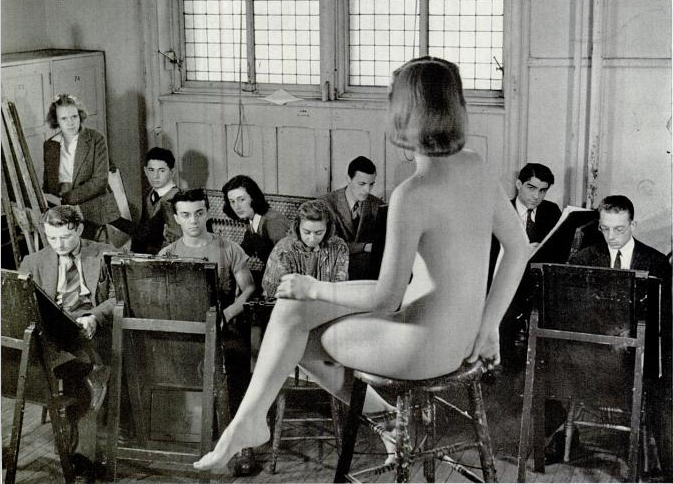
\includegraphics[width=0.65\linewidth]{./images/yaleartschool.png}
\caption{. . . caption . . . }
\end{Photo}



Note that after each such definition, a new 
environment will be available. Naturally,
its name depends on the `type' (e.g., the example code above will create the program
environment). The `float style' can be specified with the \cs{floatstyle} command. The
command takes only one argument, which is the name of a ‘‘float style’’:

\begin{teX}
\begin{Example}
     First verbatim line.
     Second verbatim line.
     Third verbatim line.
\end{Example}
\end{teX}

Float environments defined with \docAuxCommand{newfloat} do not respect the position of the 
\refCom{caption} command but always use the selected float style instead which have a fixed, pre-defined caption position. They behave differently regarding this aspect than figure and table. (BTW: To make figure and table behave like environments defined with |\newfloat|, the float package offers \docAux{restylefloat}.)

So if you want to have a floating environment which behaves like figure and table and let you place the |\caption| where you want to, do not use |\newfloat| but |\DeclareFloatingEnvironment| (or |\DeclareCaptionType|) offered by the \pkg{newfloat} package, or |\DeclareNewTOC| offered by the KOMA-Script document classes.\footnote{
\protect\url{https://tex.stackexchange.com/questions/115499/image-caption-within-newfloat}}


\endinput

\floatstyle{ruled}
\newfloat{Example}{htbp}{loe}[chapter]

 \begin{Example}
 \begin{verbatim}
   \begin{Photo}
      \centering
      \includegraphics[width=0.65\linewidth]{./graphics/level3.jpg}
      \caption{. . . caption . . . }
   \end{Photo}
\end{verbatim}
\caption{Example using verbatim code}
 \end{Example}

\begin{Photo}
 \centering
 \includegraphics[width=0.85\linewidth]{./images/old-timer-structural-worker.jpg}
\caption{. . . caption . . . }
\end{Photo}


                                             
\begin{plate}[h]
\caption{This is a plate}
 \end{plate}                                             


\begin{painting}[h]
\caption{This is a plate}
 \end{painting} 


\let\HUGE\Huge    
\cxset{part format=stewart,part afterindent=on}
\part{Latex Classes}
\let\HUGE\Huge
%\part{The \LaTeX\ standard class}

\setlength\columnsep{2em}
\def\Paragraph#1{{\bfseries #1}\quad}
\let\sidenote\footnote
\chapter{The book.cls}
\label{ch:bookclass}
\index{classes>standard}
\index{book>class}


\clearpage

\includegraphics[width=\textwidth]{./graphics/anatomy.jpg}

\vspace{2\baselineskip}

\textbf{\Large DISSECTING THE BOOK CLASS}
\thispagestyle{plain}
\begin{multicols}{2}
This appendix describes the listing of the book class as defined by \latexe. It is described here with extra commentary in order to enable you to understand, how it all works.

\lipsum[1-3]
\end{multicols}

\section{General}
\pagestyle{headings}

The book class starts with declaring the version of \latex, required
and naming the class it provides. The class choices are always checked for backward compatibility with the earlier version of \latex. All commands that need to be modified between two column and one column layouts, check the setting and branch accordingly. Another primary choice is if the book is to be printed on both sides or only on one side.


\begin{teX}
\NeedsTeXFormat{LaTeX2e}[1995/12/01]
\ProvidesClass{book}
              [2007/10/19 v1.4h
 Standard LaTeX document class]
\end{teX}

\begin{docCommand}{@ptsize} { \meta{dim}}
This is set to an empty value at start up. The original idea here was by modifying the value one could scale the
text later on. I am not aware of any such usage.
\end{docCommand}

\begin{teX}
\newcommand\@ptsize{}
\newif\if@restonecol
\newif\if@titlepage \@titlepagetrue
\newif\if@openright
\newif\if@mainmatter \@mainmattertrue
\end{teX}


\Paragraph{Paper size.} After checking for compatibilty with older versions the code branches to define the different standard paper sizes! The options that are declared are, |a4paper|, |a5paper|, |b5paper|, |letterpaper|, |legalpaper| and  |executivepaper|. The class will then later on process the options and set the default to |letterpaper|. \footnote{The package \texttt{geometry}, some classes such as the |Octavo|\index{classes>Octavo} and |KOMA|\index{classes>KOMA} classes add additional sizes to cater for other standards.}

\begin{teX}
\if@compatibility\else
\DeclareOption{a4paper}
   {\setlength\paperheight {297mm}%
    \setlength\paperwidth  {210mm}}
\DeclareOption{a5paper}
   {\setlength\paperheight {210mm}%
    \setlength\paperwidth  {148mm}}
\DeclareOption{b5paper}
   {\setlength\paperheight {250mm}%
    \setlength\paperwidth  {176mm}}
\DeclareOption{letterpaper}
   {\setlength\paperheight {11in}%
    \setlength\paperwidth  {8.5in}}
\DeclareOption{legalpaper}
   {\setlength\paperheight {14in}%
    \setlength\paperwidth  {8.5in}}
\DeclareOption{executivepaper}
   {\setlength\paperheight {10.5in}%
    \setlength\paperwidth  {7.25in}}
\end{teX}

\begin{multicols}{2}
\Paragraph{Paper orientation.} the paper orientation is set based on the |landscape| option. If it is declared it stores the |\paperheight| into one of the \latex kernel scratch registers, |\@tempdima| and then reverses the length with the |\paperwidth|.
\end{multicols}


\begin{teX}
\DeclareOption{landscape}
   {\setlength\@tempdima   {\paperheight}%
    \setlength\paperheight {\paperwidth}%
    \setlength\paperwidth  {\@tempdima}}
\fi
\end{teX}


\Paragraph{Font sizing} The class provides for three font sizes |10pt|, |11pt| and |12pt|. It defaults to ten point text. It then
sets the \refCom{@ptsize} accordingly. This is used later on to determine what size of font we are using.


\begin{teX}
\if@compatibility
  \renewcommand\@ptsize{0}
\else
\DeclareOption{10pt}{\renewcommand\@ptsize{0}}
\fi
\DeclareOption{11pt}{\renewcommand\@ptsize{1}}
\DeclareOption{12pt}{\renewcommand\@ptsize{2}}
\end{teX}


\Paragraph{Recto and verso pages.} The class provides the |oneside| and |twoside| options for switching between one side printing or two side printing.  It sets the booleans \docAuxCommand{if@twoside} and |\if@mparswitch| accordingly. These conditionals are used later to setting other variables.


\begin{teX}
\if@compatibility\else
  \DeclareOption{oneside}{\@twosidefalse \@mparswitchfalse}
\fi
\DeclareOption{twoside}{\@twosidetrue  \@mparswitchtrue}
\end{teX}


\Paragraph{Draft and final options.} The options draft and final, just set the |\overfullrule| to either 1pt or 0pt. The |\overfullrule| is a \tex command and simply prints a small vertical line to indicate overfull boxes for the attention of the author. 


\begin{teXXX}
\DeclareOption{draft}{\setlength\overfullrule{5pt}}
\if@compatibility\else
  \DeclareOption{final}{\setlength\overfullrule{0pt}}
\fi
\end{teXXX}


\Paragraph{Title page option.} If the book class, needed such an option is debatable. The |titlepage| option is normally set as true and results in the title being on its own page. The |notitlepage| will omit the page break and display the title on the same page with that of the opening text. Highly unlikely for any author to use it for a book. It is useful for the article class.


\begin{teX}
\DeclareOption{titlepage}{\@titlepagetrue}
\if@compatibility\else
  \DeclareOption{notitlepage}{\@titlepagefalse}
\fi
\end{teX}


\Paragraph{Display of chapters.} Chapters can be set to start only on an even page or any page. The class provides the options |openright| and |openany|.


\begin{teX}
\if@compatibility
  \@openrighttrue
\else
  \DeclareOption{openright}{\@openrighttrue}
  \DeclareOption{openany}{\@openrightfalse}
\fi
\end{teX}



\begin{teX}
\if@compatibility\else
 \DeclareOption{onecolumn}{\@twocolumnfalse}
\fi
\DeclareOption{twocolumn}{\@twocolumntrue} 
\DeclareOption{leqno}{\input{leqno.clo}}
\DeclareOption{fleqn}{\input{fleqn.clo}}
\DeclareOption{openbib}{%
  \AtEndOfPackage{%
   \renewcommand\@openbib@code{%
      \advance\leftmargin\bibindent
      \itemindent -\bibindent
      \listparindent \itemindent
      \parsep \z@
      }%
   \renewcommand\newblock{\par}}%
}
\end{teX}

At this point all the options have been declared and we can process them, using \refCom{ExecuteOptions} and \refCom{ProcessOptions}.

\begin{teX}
\ExecuteOptions{letterpaper,10pt,twoside,onecolumn,final,openright}
\ProcessOptions
\end{teX}


\textbf{The .clo files}\quad The book class now inputs the file |.clo| etc that defines the fontsizes
 for anything specific to the 10pt. These files hold quite a bit of information and size related commands for the
standard sizes provided by \latex. The |.clo| files also set many other parameters for page sizing, lists, paper sectioning, such as margins, marginpars and the like.


\begin{teX}
\input{bk1\@ptsize.clo}
\setlength\lineskip{1\p@}
\setlength\normallineskip{1\p@}
\renewcommand\baselinestretch{}
\setlength\parskip{0\p@ \@plus \p@}
\end{teX}


\Paragraph{Penalties.} Next we set some penalties. The definition of \refCom{@lowpenalty}, \refCom{@medpenalty} and \refCom{@highpenealty} are in the kernel in the |ltfinal| |.dtx| file.

\begin{teX}
\@lowpenalty   51
\@medpenalty  151
\@highpenalty 301
\end{teX}


\textbf{Float control parameters.}\quad The allowable number of floats on a page are controlled by a number of parameters. These are set here. Many users overwrite these parameters in order to have more control on the placement of floats.


\begin{teX}
\setcounter{topnumber}{2}
\renewcommand\topfraction{.7}
\setcounter{bottomnumber}{1}
\renewcommand\bottomfraction{.3}
\setcounter{totalnumber}{3}
\renewcommand\textfraction{.2}
\renewcommand\floatpagefraction{.5}
\setcounter{dbltopnumber}{2}
\renewcommand\dbltopfraction{.7}
\renewcommand\dblfloatpagefraction{.5}
\end{teX}


\textbf{Running head and foot.}\quad A page header or simply header in typography is text which is separated from the main body of text and appears at the top of a printed page. Word processing programs usually provide for the creation and maintenance of page headers, which are often the same from page to page, with merely small differences in information, such as page number.

In publishing, the page header (or ``pagehead'') is often referred to as the running head. Typical running heads in a book might consist of the book title on the left-hand (verso) page, and the chapter title on the right-hand (recto) page, or chapter title on the verso and subsection title on the recto.


\section{Running Heads}

\begin{teXXX}
\if@twoside
  \def\ps@headings{%
      \let\@oddfoot\@empty\let\@evenfoot\@empty
      \def\@evenhead{\thepage\hfil\slshape\leftmark}%
      \def\@oddhead{{\slshape\rightmark}\hfil\thepage}%
      \let\@mkboth\markboth
 % chapter
  \def\chaptermark##1{%
      \markboth {\MakeUppercase{%
        \ifnum \c@secnumdepth >\m@ne
          \if@mainmatter
            \@chapapp\ \thechapter. \ %
          \fi
        \fi
        ##1}}{}}%
% section
    \def\sectionmark##1{%
      \markright {\MakeUppercase{%
        \ifnum \c@secnumdepth >\z@
          \thesection. \ %
        \fi
        ##1}}}}
\else
  \def\ps@headings{%
    \let\@oddfoot\@empty
    \def\@oddhead{{\slshape\rightmark}\hfil\thepage}%
    \let\@mkboth\markboth
    \def\chaptermark##1{%
      \markright {\MakeUppercase{%
        \ifnum \c@secnumdepth >\m@ne
          \if@mainmatter
            \@chapapp\ \thechapter. \ %
          \fi
        \fi
        ##1}}}}
\fi
\def\ps@myheadings{%
    \let\@oddfoot\@empty\let\@evenfoot\@empty
    \def\@evenhead{\thepage\hfil\slshape\leftmark}%
    \def\@oddhead{{\slshape\rightmark}\hfil\thepage}%
    \let\@mkboth\@gobbletwo
    \let\chaptermark\@gobble
    \let\sectionmark\@gobble
    }
\end{teXXX}


Please note the \refCom{ps@plain} headings are not defined in the class. These are defined in the \latex kernel\footnote{See \texttt{File J: ltpage.dtx} \pageref{kernel:ltpgage}.}

\begin{teX}
\ps@plain The plain page style: No head, centred page number in foot.
13 \def\ps@plain{\let\@mkboth\@gobbletwo
14 \let\@oddhead\@empty\def\@oddfoot{\reset@font\hfil\thepage
15 \hfil}\let\@evenhead\@empty\let\@evenfoot\@oddfoot}
\end{teX}



\textbf{Title pages.}\quad Title pages are defined between a conditional, that handle the option |titlepage|
and. The commands just take mostly of the typography. If you use the option |notitlepage| in the book class, the title will be similar for all practical purposes to that of an |article| and it will appear on the top of the first page.

The |\maketitle| sets the |\footnotesise|, the |\footnoterule| and the |\footnote|.


\Paragraph{Titlepage} 

\begin{teX}
 \if@titlepage
  \newcommand\maketitle{\begin{titlepage}%
  \let\footnotesize\small
  \let\footnoterule\relax
  \let \footnote \thanks
  \null\vfil
  \vskip 60\p@
  \begin{center}%
    {\LARGE \@title \par}%
    \vskip 3em%
    {\large
     \lineskip .75em%
      \begin{tabular}[t]{c}%
        \@author
      \end{tabular}\par}%
      \vskip 1.5em%
    {\large \@date \par}%       % Set date in \large size.
  \end{center}\par
  \@thanks
  \vfil\null
  \end{titlepage}%
  \setcounter{footnote}{0}%
  \global\let\thanks\relax
  \global\let\maketitle\relax
  \global\let\@thanks\@empty
  \global\let\@author\@empty
  \global\let\@date\@empty
  \global\let\@title\@empty
  \global\let\title\relax
  \global\let\author\relax
  \global\let\date\relax
  \global\let\and\relax
}
\else
\newcommand\maketitle{\par
  \begingroup
    \renewcommand\thefootnote{\@fnsymbol\c@footnote}%
    \def\@makefnmark{\rlap{\@textsuperscript{\normalfont\@thefnmark}}}%
    \long\def\@makefntext##1{\parindent 1em\noindent
            \hb@xt@1.8em{%
                \hss\@textsuperscript{\normalfont\@thefnmark}}##1}%
    \if@twocolumn
      \ifnum \col@number=\@ne
        \@maketitle
      \else
        \twocolumn[\@maketitle]%
      \fi
    \else
      \newpage
      \global\@topnum\z@   % Prevents figures from going at top of page.
      \@maketitle
    \fi
    \thispagestyle{plain}\@thanks
  \endgroup
  \setcounter{footnote}{0}%
  \global\let\thanks\relax
  \global\let\maketitle\relax
  \global\let\@maketitle\relax
  \global\let\@thanks\@empty
  \global\let\@author\@empty
  \global\let\@date\@empty
  \global\let\@title\@empty
  \global\let\title\relax
  \global\let\author\relax
  \global\let\date\relax
  \global\let\and\relax
}
\def\@maketitle{%
  \newpage
  \null
  \vskip 2em%
  \begin{center}%
  \let \footnote \thanks
    {\LARGE \@title \par}%
    \vskip 1.5em%
    {\large
      \lineskip .5em%
      \begin{tabular}[t]{c}%
        \@author
      \end{tabular}\par}%
    \vskip 1em%
    {\large \@date}%
  \end{center}%
  \par
  \vskip 1.5em}
\fi
\end{teX}


\Paragraph{Section counters.}\quad 
In LaTeX all defaults all document section are numbered by default. These numbers are kept in counters, named after the section name. A series of commands are provided to access these numbers.
All the counters are in arabic numerals, with the exception of "part", which is in Roman.


\begin{teX}
\newcommand*\chaptermark[1]{}
\setcounter{secnumdepth}{2}
\newcounter {part}
\newcounter {chapter}
\newcounter {section}[chapter]
\newcounter {subsection}[section]
\newcounter {subsubsection}[subsection]
\newcounter {paragraph}[subsubsection]
\newcounter {subparagraph}[paragraph]
\renewcommand \thepart {\@Roman\c@part}
\renewcommand \thechapter {\@arabic\c@chapter}
\renewcommand \thesection {\thechapter.\@arabic\c@section}
\renewcommand\thesubsection   {\thesection.\@arabic\c@subsection}
\renewcommand\thesubsubsection{\thesubsection.\@arabic\c@subsubsection}
\renewcommand\theparagraph    {\thesubsubsection.\@arabic\c@paragraph}
\renewcommand\thesubparagraph {\theparagraph.\@arabic\c@subparagraph}
\newcommand\@chapapp{\chaptername}
\end{teX}


\textbf{Frontmatter, mainmatter and backmatter.} These are author command to set mostly, the page numbering and the clearing of pages for two page layouts. Front matter has lower roman pages numbering and the main matter has arabic numerals.

\begin{docCommand}{frontmatter}{}
Front matter sets the page opening and teh numbering in Roman lowercase.
\end{docCommand}

\emphasis{frontmatter,mainmatter,backmatter}
\begin{teX}
\newcommand\frontmatter{%
    \cleardoublepage
  \@mainmatterfalse
  \pagenumbering{roman}}
\end{teX}

\begin{docCommand}{mainmatter} The author command to denote the start of the main body of the publication.
\end{docCommand}
\begin{teX}
\newcommand\mainmatter{%
    \cleardoublepage
  \@mainmattertrue
  \pagenumbering{arabic}}
\end{teX}

\begin{docCommand}{backmatter} The author command to denote the start of the back matter of the publication. These are still
numbered in arabic numerals.
\end{docCommand}
\begin{teX}
\newcommand\backmatter{%
  \if@openright
    \cleardoublepage
  \else
    \clearpage
  \fi
  \@mainmatterfalse}
\end{teX}


\Paragraph{Part.}The is the definition of part. The Part is displayed with a plain header and the it goes into the secdef. If the section depth is greater or equal -2, the start counter is increased and the part is added to the toc, using |\addcontentsline|. 
The partname i.e., default 'Part' gets printer either way except for the star version of the command.

\begin{docCommand}{part}{}
Starts a new part of a book. The star version of the command does not increment the part number.
\end{docCommand}


\emphasis{@part,@spart,secdef}
\begin{teXXX}
\newcommand\part{%
  \if@openright
    \cleardoublepage
  \else
    \clearpage
  \fi
  \thispagestyle{plain}%
  \if@twocolumn
    \onecolumn
    \@tempswatrue
  \else
    \@tempswafalse
  \fi
  \null\vfil
  \secdef\@part\@spart}
\end{teXXX}


 The important command to remember here
is \refCom{secdef}. This is defined in the kernel and not in the classes \texttt{ltsect.dtx}. Essentially in the code |\@part| calls the unstar command and the @spart calls the starred command. We copy the definition from the kernel for convenience.


\begin{teXXX}
is \secdef{unstarcmds}{unstarcmds}{starcmds}
When defining a \chapter or \section command without using \@startsection,
you can use \secdef as follows:
1. \def\chapter{ . . . \secdef \starcmd \unstarcmd}
2. \def\hstarcmdi[#1]#2{ . . . } % Command to define \chapter[. . . ]{. . . }
3. \def\unstarcmd#1{ . . . } % Command to define \chapter*{. . . }
125 \def\secdef#1#2{\@ifstar{#2}{\@dblarg{#1}}}
\end{teXXX}

The |@part| starts now,

\begin{teXXX}
\def\@part[#1]#2{%
    \ifnum \c@secnumdepth >-2\relax
      \refstepcounter{part}%
      \addcontentsline{toc}{part}{\thepart\hspace{1em}#1}%
    \else
      \addcontentsline{toc}{part}{#1}%
    \fi
    \markboth{}{}%
    {\centering
     \interlinepenalty \@M
     \normalfont
     \ifnum \c@secnumdepth >-2\relax
       \huge\bfseries \partname\nobreakspace\thepart
       \par
       \vskip 20\p@
     \fi
     \Huge \bfseries #2\par}%
    \@endpart}
\end{teXXX}

\begin{multicols}{2}
The starred version of the command is provided next. The difference the name `Part'' is not displayed. However the parameter provided by the user is displayed. A normal font is provided. Final settings depending on @openright and header styles are set and the code macro is completed.
\end{multicols}

\begin{teXXX}
\def\@spart#1{%
    {\centering
     \interlinepenalty \@M
     \normalfont
     \Huge \bfseries #1\par}%
    \@endpart}

\def\@endpart{\vfil\newpage
              \if@twoside
               \if@openright
                \null
                \thispagestyle{empty}%
                \newpage
               \fi
              \fi
              \if@tempswa
                \twocolumn
              \fi}
\end{teXXX}


\Paragraph{Chapter}. The chapter definition follows, the same pattern as that of the part definitions. It calls secdef and defines commands for the starred and unstarred versions.


\begin{teXXX}
\newcommand\chapter{\if@openright\cleardoublepage\else\clearpage\fi
                    \thispagestyle{plain}%
                    \global\@topnum\z@
                    \@afterindentfalse
                    \secdef\@chapter\@schapter}
\end{teXXX}

\Paragraph{Unstarred version}

\begin{teXXX}
\def\@chapter[#1]#2{
    \ifnum \c@secnumdepth >\m@ne
       \if@mainmatter
             \refstepcounter{chapter}%
             \typeout{\@chapapp\space\thechapter.}%
             \addcontentsline{toc}{chapter}%
             {\protect\numberline{\thechapter}#1}%
       \else
             \addcontentsline{toc}{chapter}{#1}%
      \fi
   \else
         \addcontentsline{toc}{chapter}{#1}%
   \fi
   \chaptermark{#1}%
   \addtocontents{lof}{\protect\addvspace{10\p@}}%
   \addtocontents{lot}{\protect\addvspace{10\p@}}%
   \if@twocolumn
        \@topnewpage[\@makechapterhead{#2}]%
   \else
        \@makechapterhead{#2}%
        \@afterheading
   \fi}
\end{teXXX}

\begin{multicols}{2}
\Paragraph{Defining the looks of the Chapter heading.}

Good practice dictates, that when you change the chapterhead layout for the numbered version, you also change it for the star version of the command. You can do that by using two different macros, although at first glance it might be difficult to see where the difference is.
\end{multicols}


\emphasis{@makeschapterhead,@makechapterhead}
\begin{teXXX}
\def\@makechapterhead
\def\@makeschapterhead
\end{teXXX}

\begin{teXXX}
\def\@makechapterhead#1{%
  \vspace*{50\p@}%
  {\parindent \z@ \raggedright \normalfont
    \ifnum \c@secnumdepth >\m@ne
      \if@mainmatter
        \huge\bfseries \@chapapp\space \thechapter
        \par\nobreak
        \vskip 20\p@
      \fi
    \fi
    \interlinepenalty\@M
    \Huge \bfseries #1\par\nobreak
    \vskip 40\p@
  }}
\end{teXXX}


Finally the starred version of the command is called. This now checks for twocolumn or one column via an if sttaement and executes, the makeschapterhead. Another mysterious and wonderful command appears again from the LaTeX source2e.\cmd{\@afterheading}. This command 
is just a hook for custom headings? (Needs to be reviewed again).


\begin{teXXX}
\def\@schapter#1{\if@twocolumn
                   \@topnewpage[\@makeschapterhead{#1}]%
                 \else
                   \@makeschapterhead{#1}%
                   \@afterheading
                 \fi}
\end{teXXX}

And finally the |\@makeschapterhead| (remember \textbf{s} for \textbf{s}tar).

\begin{teXXX}
\def\@makeschapterhead#1{%
  \vspace*{50\p@}%
  {\parindent \z@ \raggedright
    \normalfont
    \interlinepenalty\@M
    \Huge \bfseries  #1\par\nobreak
    \vskip 40\p@
  }}
\end{teXXX}

All sorts of variations of the above two commands can be found in different classes, such as |KOMA|, |memoir| and others. The example which follows, typesets the headings as shown in \fref{fig:chapterhead-17}. The |@makechapterhead| command is modified to produce a centered heading which is displayed between two heavy rules. This style can be found in quite a number of books.

\begin{figure*}[htbp]
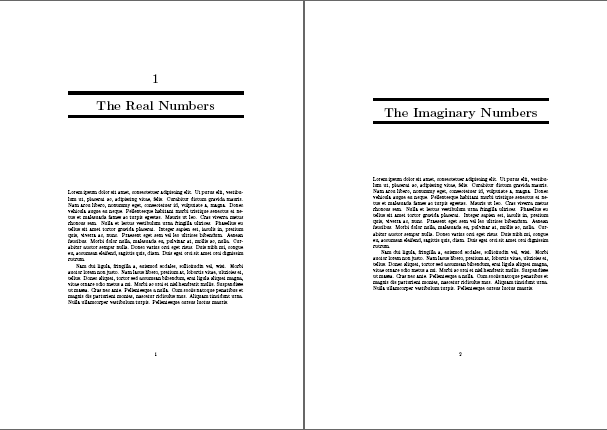
\includegraphics[width=\linewidth]{./graphics/chapterhead-17.png}
\caption{Modifying the way the chapterhead looks can be achieved by redefining the \texttt{\textbackslash @makechapterhead} and \texttt{\textbackslash @makeschapterhead} commands.}
\label{fig:chapterhead-17}
\end{figure*}

\section*{Full working example}

\begin{teX}
\documentclass[oneside]{book}
\usepackage[english]{babel}
\usepackage{lipsum}
\makeatletter
\def\thickhrule{\leavevmode \leaders \hrule height 1ex \hfill \kern \z@}

%% Note the difference between the commands the one is 
%% make and the other one is makes
\renewcommand{\@makechapterhead}[1]{%
  \vspace*{10\p@}%
  {\parindent \z@ \centering \reset@font
        {\Huge \scshape  \thechapter }
        \par\nobreak
        \vspace*{10\p@}%
        \interlinepenalty\@M
        \thickhrule
        \par\nobreak
        \vspace*{2\p@}%
        {\Huge \bfseries #1\par\nobreak}
        \par\nobreak
        \vspace*{2\p@}%
        \thickhrule
    \vskip 40\p@
    \vskip 100\p@
  }}

%% This is makes
\def\@makeschapterhead#1{%
  \vspace*{10\p@}%
  {\parindent \z@ \centering \reset@font
        {\Huge \scshape \vphantom{\thechapter}}
        \par\nobreak
        \vspace*{10\p@}%
        \interlinepenalty\@M
        \thickhrule
        \par\nobreak
        \vspace*{2\p@}%
        {\Huge \bfseries #1\par\nobreak}
        \par\nobreak
        \vspace*{2\p@}%
        \thickhrule
    \vskip 100\p@
  }}
\begin{document}
\chapter{The Real Numbers}
\lipsum[1-2]
\chapter*{The Imaginary Numbers}
\lipsum[1-2]
\end{document}
\end{teX}


\Paragraph{The sections.}
In this section, all the document elements besides the Chapter and the Part are Defined. They use the mother of all commands from the kernel
ltsection.dtx, named \refCom{@startsection}. This is just a call to the kernel command. No other settings are done here. In order to remember what it does we refer to its definition in the kernel. Of interest is the sixth argument which sets the font style.

The parameter takes eight parameters, some of them optional. We discuss this command in more detail in the kernel chapter.



\emphasis{@startsection}
\begin{teX}
\newcommand\section{\@startsection {section}{1}{\z@}%
                                   {-3.5ex \@plus -1ex \@minus -.2ex}%
                                   {2.3ex \@plus.2ex}%
                                   {\normalfont\Large\bfseries}}
\newcommand\subsection{\@startsection{subsection}{2}{\z@}%
                                     {-3.25ex\@plus -1ex \@minus -.2ex}%
                                     {1.5ex \@plus .2ex}%
                                     {\normalfont\large\bfseries}}
\newcommand\subsubsection{\@startsection{subsubsection}{3}{\z@}%
                                     {-3.25ex\@plus -1ex \@minus -.2ex}%
                                     {1.5ex \@plus .2ex}%
                                     {\normalfont\normalsize\bfseries}}
\newcommand\paragraph{\@startsection{paragraph}{4}{\z@}%
                                    {3.25ex \@plus1ex \@minus.2ex}%
                                    {-1em}%
                                    {\normalfont\normalsize\bfseries}}
\newcommand\subparagraph{\@startsection{subparagraph}{5}{\parindent}%
                                       {3.25ex \@plus1ex \@minus .2ex}%
                                       {-1em}%
                                      {\normalfont\normalsize\bfseries}}
\end{teX}                                      
\section{Lists}                                      
\label{sec:booklists}
\begin{teX}
\if@twocolumn
  \setlength\leftmargini  {2em}
\else
  \setlength\leftmargini  {2.5em}
\fi
\leftmargin  \leftmargini
\setlength\leftmarginii  {2.2em}
\setlength\leftmarginiii {1.87em}
\setlength\leftmarginiv  {1.7em}
\if@twocolumn
  \setlength\leftmarginv  {.5em}
  \setlength\leftmarginvi {.5em}
\else
  \setlength\leftmarginv  {1em}
  \setlength\leftmarginvi {1em}
\fi
\setlength  \labelsep  {.5em}
\setlength  \labelwidth{\leftmargini}
\addtolength\labelwidth{-\labelsep}
\@beginparpenalty -\@lowpenalty
\@endparpenalty   -\@lowpenalty
\@itempenalty     -\@lowpenalty
\renewcommand\theenumi{\@arabic\c@enumi}
\renewcommand\theenumii{\@alph\c@enumii}
\renewcommand\theenumiii{\@roman\c@enumiii}
\renewcommand\theenumiv{\@Alph\c@enumiv}
\newcommand\labelenumi{\theenumi.}
\newcommand\labelenumii{(\theenumii)}
\newcommand\labelenumiii{\theenumiii.}
\newcommand\labelenumiv{\theenumiv.}
\renewcommand\p@enumii{\theenumi}
\renewcommand\p@enumiii{\theenumi(\theenumii)}
\renewcommand\p@enumiv{\p@enumiii\theenumiii}
\newcommand\labelitemi{\textbullet}
\newcommand\labelitemii{\normalfont\bfseries \textendash}
\newcommand\labelitemiii{\textasteriskcentered}
\newcommand\labelitemiv{\textperiodcentered}
\end{teX}


\section{The description Environment}

\begin{docCommand}{descriptionlabel}{\marg{\meta{text}}}
\end{docCommand}

\begin{teX}
\newenvironment{description}
               {\list{}{\labelwidth\z@ \itemindent-\leftmargin
                        \let\makelabel\descriptionlabel}}
               {\endlist}
               
\newcommand*\descriptionlabel[1]{\hspace\labelsep
                                \normalfont\bfseries #1}
\end{teX}

\section{Verse Environment}
\label{sec:verseenvironment}
\textbf{The verse environment}\quad \latex's \docAuxEnvironment{verse} environment, can only serve for the incidental use of a few stanzas. It leaves most of the formatting to the author.  It redefines the line break |\\| to a |\centercr|.


\begin{teX}
\newenvironment{verse}
    {\let\\\@centercr(*@\protect\footnote{This is defined in ltmiscen.dtx}@*)
     \list{}{\itemsep  \z@
             \itemindent   -1.5em%
             \listparindent\itemindent
             \rightmargin  \leftmargin
             \advance\leftmargin 1.5em}%
       \item\relax}
    {\endlist}
\end{teX}
\makeatletter
\newenvironment{Verse}
    {\let\\\@centercr%
     \list{}{\itemsep1pt
             \itemindent-1.5em%
             \listparindent\itemindent
             \rightmargin\leftmargin
             \advance\leftmargin 1.5em}%
       \item\relax}
    {\endlist}
\makeatother
\begin{teX}
  \begin{Verse}
     My mobile test\\
     this is other\\
     this is last\\
  \end{Verse}
\end{teX}

The environment doesn't really do much, the way I see it but just move the poem a couple of ems inwards 
to much the definition of lists. Most people will want more from a poem environment.
\begin{Verse}
     My mobile test\\
      this is other\\
       this is last\\
\end{Verse}

The simplest thing we can add to this environment if we want to modify it, is a hook. This we can do using the |blckcntrl| package. \sidenote{From the \url{http://www.ifi.uio.no/it/latex-links/blkcntrl.pdf}}.

\begin{teX}
\renewenvironment{verse}
50 {\let\\\@centercr
51 \relax\list{}{\setlength{\itemsep}{\z@}%
52 \setlength{\itemindent}{-1.5em}%
53 \setlength{\listparindent}{\itemindent}%
54 \setlength{\rightmargin}{\leftmargin}%
55 \addtolength{\leftmargin}{1.5em}}%
56 \item\relax\PreVerse\relax}
57 {\endlist}
\end{teX}

Using the command |\PreVerse|, we can add a block at the beginning of the block. For example some code to make a poem title and insert it later on. The setting of the rightmargin to the leftmargin here is curious. It might for example give us problems with |tufte-latex| classes.


\section{Quotation and quote environments}
\label{sec:quotationenvironment}

\textbf{The quote and quotation environments.}\quad The environments |quote| and |quotation| are defined next. Again they are defined using the general \refCom{list} environment. Again the general |\list|, is used in the definition. The dimension \refCom{listparindent} is set to 1.5 em. (See Kernel file |ltlists.dtx| \ref{kernel:ltlists}). 


\begin{teX}
\newenvironment{quotation}
               {\list{}{\listparindent 1.5em%
                        \itemindent\listparindent
                        \rightmargin\leftmargin
                        \parsep\z@ \@plus\p@}%
                \item\relax}
               {\endlist}
\end{teX}

\begin{teX}
\newenvironment{quote}
               {\list{}{\rightmargin\leftmargin}%
                \item\relax}
               {\endlist}




\section{The \protect\texttt{titlepage} environment}
\if@compatibility
\newenvironment{titlepage}
    {%
      \cleardoublepage
      \if@twocolumn
        \@restonecoltrue\onecolumn
      \else
        \@restonecolfalse\newpage
      \fi
      \thispagestyle{empty}%
      \setcounter{page}\z@
    }%
    {\if@restonecol\twocolumn \else \newpage \fi
    }
\else
\newenvironment{titlepage}
    {%
      \cleardoublepage
      \if@twocolumn
        \@restonecoltrue\onecolumn
      \else
        \@restonecolfalse\newpage
      \fi
      \thispagestyle{empty}%
      \setcounter{page}\@ne
    }%
    {\if@restonecol\twocolumn \else \newpage \fi
     \if@twoside\else
        \setcounter{page}\@ne
     \fi
    }
\fi
\end{teX}




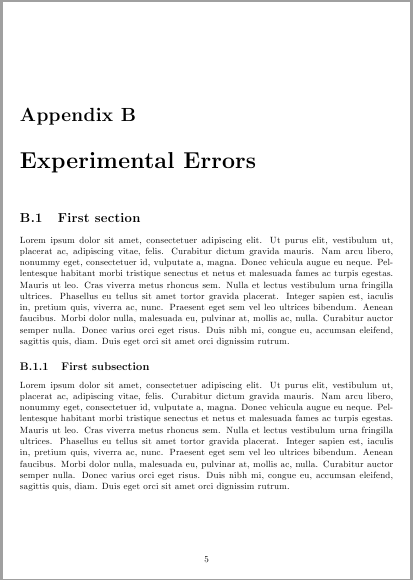
\includegraphics[width=\linewidth]{./graphics/appendix.png}

\Paragraph{The Appendix.}
Similarly to the chapter sectioning commands, the Appendix is not defined as a section. It simply sets the chapter and section counters to zero and sets the name of the section. All the relevant counters and uses letters for the numbering of the following chapters etc. If you closely follow the code, it is all based on the chapter command, except that it defaults to Alphanumeric counting.

\begin{docCommand}{appendix}{}
\end{docCommand}

\emphasis[thegreen]{appendix}
\begin{teX}
\newcommand\appendix{\par
  \setcounter{chapter}{0}%
  \setcounter{section}{0}%
  \gdef\@chapapp{\appendixname}(*@\sidenote{The actual literal used for \textbackslash{appendixname} is defined later on, so that you can customize the language}\label{appendixname}@*)
  \gdef\thechapter{\@Alph\c@chapter}}
\end{teX}

An Appendix page has the same looks and feel to that of a Chapter. For all practical purposes, it is a chapter, with different labels and uppecase letters numbering.



\Paragraph{General Settings.} Here, some general settings are set. These include settings for framed boxes, tabbing separators and array column separators.

\begin{teXXX}
\setlength\arraycolsep{5\p@}
\setlength\tabcolsep{6\p@}
\setlength\arrayrulewidth{.4\p@}
\setlength\doublerulesep{2\p@}
\setlength\tabbingsep{\labelsep}
\skip\@mpfootins = \skip\footins
\end{teXXX}

The \refCom{fboxsep} and \refCom{fboxrule} are then set to 3pt and .4pt respectively. These are used with frame boxes.

\begin{teXXX}
\setlength\fboxsep{3\p@}
\setlength\fboxrule{.4\p@}
\end{teXXX}


\Paragraph{Equation numbering}
The equation counter is reset according to the chapter counter, using the \latex kernel command |\@addtoreset|. 

\begin{teX}
\@addtoreset {equation}{chapter}
\renewcommand\theequation
  {\ifnum \c@chapter>\z@ \thechapter.\fi \@arabic\c@equation}
\end{teX}

\section{FIGURE AND TABLE ENVIRONMENTS}


\Paragraph{Figure Environment} The figure environment is defined using commands that have been provided by the kernel.  The command |\thefigure| is first redefined to display the combination of the chapter dot figure counter, all in arabic numerals. The extension for the list of figures and finally the floats for single column and double column.



\label{book:figure}
\begin{teX}
\newcounter{figure}[chapter]
\renewcommand \thefigure
     {\ifnum \c@chapter>\z@ \thechapter.\fi \@arabic\c@figure}
\def\fps@figure{tbp}
\def\ftype@figure{1}
\def\ext@figure{lof}
\def\fnum@figure{\figurename\nobreakspace\thefigure}
\newenvironment{figure}
               {\@float{figure}}
               {\end@float}
\newenvironment{figure*}
               {\@dblfloat{figure}}
               {\end@dblfloat}
\end{teX}




\begin{multicols}{2}
\Paragraph{Table Environment} Table floats are defined the same way like the figures with their respective counters and names.  
\end{multicols}

\begin{teX}
\newcounter{table}[chapter]
\renewcommand \thetable
     {\ifnum \c@chapter>\z@ \thechapter.\fi \@arabic\c@table}
\def\fps@table{tbp}
\def\ftype@table{2}
\def\ext@table{lot}
\def\fnum@table{\tablename\nobreakspace\thetable}


\newenvironment{table}
               {\@float{table}}
               {\end@float}

\newenvironment{table*}
               {\@dblfloat{table}}
               {\end@dblfloat}
\end{teX}

\begin{multicols}{2}
\Paragraph{Captions}
The captioning macros are rather short but need a bit of explanation. First
some lengths are defined. The lengths are for |abovecaptionskip| and |belowcaptionskip| are set equal to a default of 10pt as for the font-size, but the length |belowcaptionskip| is set to |opt|.
\end{multicols}

\begin{teX}
\newlength\abovecaptionskip
\newlength\belowcaptionskip
\setlength\abovecaptionskip{10\p@}
\setlength\belowcaptionskip{0\p@}

\long\def\@makecaption#1#2{%
  \vskip\abovecaptionskip
  \sbox\@tempboxa{#1: #2}
  \ifdim \wd\@tempboxa >\hsize
    #1: #2\par
  \else
    \global \@minipagefalse
    \hb@xt@\hsize{\hfil\box\@tempboxa\hfil}%
  \fi
  \vskip\belowcaptionskip}
\end{teX}

\begin{multicols}{2}
The |@makecaption| macro is also interesting. Firstly note in line  the use of a colon (:). So if you do not like to have this you know where you need to go and change it. The contents of the caption are first saved into a box. If the box is greater than |hsize| then they are written like a paragraph otherwise, they are centered. Note that the centering is done using |\hfil\box\@tempoxa\hfil|. The mysterious command |\hb@xt| is defined in the kernel and
is equivalent to |\hbox to|
\end{multicols}

\begin{teXXX}
  \hb@xt@ The next one is another 100 tokens worth.
  16 \def\hb@xt@{\hbox to}
\end{teXXX}

\begin{multicols}{2}
It is simply an abbreviation of |\hbox to|. There are many short-cut commands like this, so the command just again sets the caption in a  horizontal box. There is more to the story later on. 
\end{multicols}


\section{Defining the old style font commands}

\begin{teX}
\DeclareOldFontCommand{\rm}{\normalfont\rmfamily}{\mathrm}
\DeclareOldFontCommand{\sf}{\normalfont\sffamily}{\mathsf}
\DeclareOldFontCommand{\tt}{\normalfont\ttfamily}{\mathtt}
\DeclareOldFontCommand{\bf}{\normalfont\bfseries}{\mathbf}
\DeclareOldFontCommand{\it}{\normalfont\itshape}{\mathit}
\DeclareOldFontCommand{\sl}{\normalfont\slshape}{\@nomath\sl}
\DeclareOldFontCommand{\sc}{\normalfont\scshape}{\@nomath\sc}
\DeclareRobustCommand*\cal{\@fontswitch\relax\mathcal}
\DeclareRobustCommand*\mit{\@fontswitch\relax\mathnormal}
\end{teX}


\section{Table of contents}


Firstly we define the width of the box that the page number is set. Use ems so that it does not need to be redefined for every change in font size.
Toc entries are treated as rectangular areas where the text
and probably a filler will be written. Let's draw such an
area (of course, the lines themselves are not printed):



\setlength{\unitlength}{1cm}
\begin{center}
\begin{picture}(8,2.2)
\put(1,1){\line(1,0){6}}
\put(1,2){\line(1,0){6}}
\put(1,1){\line(0,1){1}}
\put(7,1){\line(0,1){1}}
\put(0,.7){\vector(1,0){1}}
\put(8,.7){\vector(-1,0){1}}
\put(0,.2){\makebox(1,.5)[b]{\textit{left}}}
\put(7,.2){\makebox(1,.5)[b]{\textit{right}}}
\end{picture}
\end{center}

The space between the left page margin and the left edge of
the area will be named |<left>|; similarly we have |<right>|.
You are allowed to modify the beginning of the first line and
the ending of the last line. For example by ``taking up'' both
places with |\hspace*{2pc}| the area becomes:
\begin{center}
\begin{picture}(8,2.2)
\put(1,1){\line(1,0){5.5}}
\put(6.5,1){\line(0,1){.5}}
\put(6.5,1.5){\line(1,0){.5}}
\put(1.5,2){\line(1,0){5.5}}
\put(1,1.5){\line(1,0){.5}}
\put(1.5,1.5){\line(0,1){.5}}
\put(1,1){\line(0,1){.5}}
\put(7,1.5){\line(0,1){.5}}
\put(0,.7){\vector(1,0){1}}
\put(8,.7){\vector(-1,0){1}}
\put(0,.2){\makebox(1,.5)[b]{\textit{left}}}
\put(7,.2){\makebox(1,.5)[b]{\textit{right}}}
\end{picture}
\end{center}
And by ``clearing'' space in both places with |\hspace*{-2pc}|
the area becomes:
\begin{center}
\begin{picture}(8,2.2)
\put(1,1){\line(1,0){6.5}}
\put(7.5,1){\line(0,1){.5}}
\put(7.5,1.5){\line(-1,0){.5}}
\put(.5,2){\line(1,0){6.5}}
\put(1,1.5){\line(-1,0){.5}}
\put(.5,1.5){\line(0,1){.5}}
\put(1,1){\line(0,1){.5}}
\put(7,1.5){\line(0,1){.5}}
\put(0,.7){\vector(1,0){1}}
\put(8,.7){\vector(-1,0){1}}
\put(0,.2){\makebox(1,.5)[b]{\textit{left}}}
\put(7,.2){\makebox(1,.5)[b]{\textit{right}}}
\end{picture}
\end{center}

\begin{multicols}{2}
If you have seen tocs, the latter should be familiar to you--
the label at the very beginning, the page at the very end:
\columnbreak

\topline
\begin{verbatim}
    3.2  This is an example showing that toc
         entries fits in that scheme . . . .   4
\end{verbatim}
\bottomline
\end{multicols}


\begin{teX}
\newcommand\@pnumwidth{1.55em}%Width of box in which page number is set.
\end{teX}

We then define the margin and the dotsep. We also set the toc counter to whatever is require (don't go too deep especially if you have an index).

\begin{teX}
\newcommand\@tocrmarg{2.55em}%Right margin indentation for all but last line of multiple-line entries.
\newcommand\@dotsep{4.5}%Separation between dots, in mu units. Should be \def'd to a number like
2 or 1.7
\end{teX}

\begin{docCommand}{tableofcontents}{}
\Paragraph{Defining the  contents table.} The author is provided with the author command |\tableofcontents|. All format information is provided at this point.
\end{docCommand}

\begin{teX}
\setcounter{tocdepth}{2}
\newcommand\tableofcontents{%
    \if@twocolumn
      \@restonecoltrue\onecolumn
    \else
      \@restonecolfalse
    \fi
    \chapter*{\contentsname
        \@mkboth{%
           \MakeUppercase\contentsname}{\MakeUppercase\contentsname}}%
    \@starttoc{toc}%
    \if@restonecol\twocolumn\fi
    }
\end{teX}

\begin{teX}
\newcommand*\l@part[2]{%
  \ifnum \c@tocdepth >-2\relax
    \addpenalty{-\@highpenalty}%
    \addvspace{2.25em \@plus\p@}%
    \setlength\@tempdima{3em}%
    \begingroup
      \parindent \z@ \rightskip \@pnumwidth
      \parfillskip -\@pnumwidth
      {\leavevmode
       \large \bfseries #1\hfil \hb@xt@\@pnumwidth{\hss #2}}\par
       \nobreak
         \global\@nobreaktrue
         \everypar{\global\@nobreakfalse\everypar{}}%
    \endgroup
  \fi}

\newcommand*\l@chapter[2]{%
  \ifnum \c@tocdepth >\m@ne
    \addpenalty{-\@highpenalty}%
    \vskip 1.0em \@plus\p@
    \setlength\@tempdima{1.5em}%
    \begingroup
      \parindent \z@ \rightskip \@pnumwidth
      \parfillskip -\@pnumwidth
      \leavevmode \bfseries
      \advance\leftskip\@tempdima
      \hskip -\leftskip
      #1\nobreak\hfil \nobreak\hb@xt@\@pnumwidth{\hss #2}\par
      \penalty\@highpenalty
    \endgroup
  \fi}
\end{teX}


The five remaining levels (entry in \latex terminology, are defined next). This is done with the general \latex kernel command 

\begin{teX}
\@dottedtocline{<level>}{<indent>}{<numwidth>}{<title>}{<page>}: Macro
to produce a table of contents line with the following parameters:
\end{teX}

The commands for the remaining sections are defined as follows:

\begin{teX}
\newcommand*\l@section{\@dottedtocline{1}{1.5em}{2.3em}}
\newcommand*\l@subsection{\@dottedtocline{2}{3.8em}{3.2em}}
\newcommand*\l@subsubsection{\@dottedtocline{3}{7.0em}{4.1em}}
\newcommand*\l@paragraph{\@dottedtocline{4}{10em}{5em}}
\newcommand*\l@subparagraph{\@dottedtocline{5}{12em}{6em}}
\end{teX}

So where are the last two parameters? These are just zeroed here!


I can assure that the |dotted| type of section bothers a lot of people. Most new books will both compact the table of contents as well as remove the dots. You can use the |titlesec| and |titletoc| to do this rather than redefining the kernel commands or the standard classes styles.

\subsection{List of figures, tables etc}
\begin{teX}
\newcommand\listoffigures{%
    \if@twocolumn
      \@restonecoltrue\onecolumn
    \else
      \@restonecolfalse
    \fi
    \chapter*{\listfigurename}%
      \@mkboth{\MakeUppercase\listfigurename}%
              {\MakeUppercase\listfigurename}%
    \@starttoc{lof}%
    \if@restonecol\twocolumn\fi
    }
\end{teX}
The interesting command here is the |@starttoc{lof}|. This simply does all the housekeeping to open a file. as you can see it is not too difficult to have file extension names other than the standard ones.

The |l@| commands for the Table of Contents are defined as per the rest of the sectioning commands.

\begin{teX}
\newcommand*\l@figure{\@dottedtocline{1}{1.5em}{2.3em}}
\newcommand\listoftables{%
    \if@twocolumn
      \@restonecoltrue\onecolumn
    \else
      \@restonecolfalse
    \fi
    \chapter*{\listtablename}%
      \@mkboth{%
          \MakeUppercase\listtablename}%
         {\MakeUppercase\listtablename}%
    \@starttoc{lot}%
    \if@restonecol\twocolumn\fi
    }
\let\l@table\l@figure
\end{teX}

\section{Bibliographies}


\latex provides some basic bibliographic commands. Every entry is defined to be displayed in a block. It starts by defining a new length |\bibindent|. Entries are displayed using the  \refCom{list}. The commands here are mainly to set parameters for macros already provide by the kernel.
\index{book>environments>thebibliography}

\begin{docEnvironment}{thebibliography}{\marg{widest label}}
\end{docEnvironment}

\begin{teX}
\newdimen\bibindent
\setlength\bibindent{1.5em}
\newenvironment{thebibliography}[1]
     {\chapter*{\bibname}%
      \@mkboth{\MakeUppercase\bibname}{\MakeUppercase\bibname}%
      \list{\@biblabel{\@arabic\c@enumiv}}%
           {\settowidth\labelwidth{\@biblabel{#1}}%
            \leftmargin\labelwidth
            \advance\leftmargin\labelsep
            \@openbib@code
            \usecounter{enumiv}%
            \let\p@enumiv\@empty
            \renewcommand\theenumiv{\@arabic\c@enumiv}}%
      \sloppy
      \clubpenalty4000
      \@clubpenalty \clubpenalty
      \widowpenalty4000%
      \sfcode`\.\@m}
     {\def\@noitemerr
       {\@latex@warning{Empty `thebibliography' environment}}%
      \endlist}
\newcommand\newblock{\hskip .11em\@plus.33em\@minus.07em}
\let\@openbib@code\@empty
\end{teX}

\section{The Index Environment}

This is a short environment definition for styling the Index. It defines in line [\ref{idxitem}] the 
|@idxidtem|, which is then used to define \docAuxCommand{subitem} and \docAuxCommand{subsubitem} styling.

\begin{teX}
\newenvironment{theindex}
   {\if@twocolumn
      \@restonecolfalse
      \else
         \@restonecoltrue
      \fi
      \twocolumn[\@makeschapterhead{\indexname}]%
      \@mkboth{\MakeUppercase\indexname}%
              {\MakeUppercase\indexname}%
                \thispagestyle{plain}\parindent\z@
                \parskip\z@ \@plus .3\p@\relax
                \columnseprule \z@
                \columnsep 35\p@
                \let\item\@idxitem}
      {\if@restonecol\onecolumn\else\clearpage\fi}
\newcommand\@idxitem{\par\hangindent 40\p@} (*@\label{idxitem}@*)
\newcommand\subitem{\@idxitem \hspace*{20\p@}}
\newcommand\subsubitem{\@idxitem \hspace*{30\p@}}
\newcommand\indexspace{\par \vskip 10\p@ \@plus5\p@ \@minus3\p@\relax}
\end{teX}

\section{Footnotes}
\label{book:footnotes}
\index{footnotes>\textbackslash footnoterule}


\begin{docCommand}{footnoterule}{}

\Paragraph{Footnote rules.} Footnote rules are defined by renewing the command |\footnoterule|. Counters for footnotes are reset based on the chapter counters. The footnote command |\@makefntext| provides the formatting. It also gives the user the ability to use these to insert footnotes, in difficult places.
\end{docCommand}




\emphasis[thegreen]{footnoterule}
\begin{teX}
\renewcommand\footnoterule{%
  \kern-3\p@
  \hrule\@width.4\columnwidth 
  \kern2.6\p@}

\@addtoreset{footnote}{chapter}
\end{teX}

\begin{docCommand}{@makefntext}{}
\end{docCommand}

\begin{docCommand}{@makefnmark}{}
\end{docCommand}

\begin{teX}
\newcommand\@makefntext[1]{%
    \parindent 1em%
    \noindent
    \hb@xt@1.8em{\hss\@makefnmark}#1}
\end{teX}

\section{Catering for Other Languages}


\textbf{Structural element names.}\quad \latex does not provide by itself the means to change the structural element names to a language other than English. Howerer, their names are defined  in a series of commands, that make it easier to be overwritten to change them to another language. As they are separate from the macros that use them, it is easy to overwrite them, in order to use another language. This is what the Babel package does. Note the Section, is not defined here.

\begin{docCommand}{contentsname}{}
Typesets the contents name.
\end{docCommand}
\begin{teX}
\newcommand\contentsname{Contents}
\end{teX}

\begin{docCommand}{listfigurename}{}
Typesets \enquote{List of Figures}, if it is not redefined.
\end{docCommand}

\begin{teX}
\newcommand\listfigurename{List of Figures}
\newcommand\listtablename{List of Tables}
\newcommand\bibname{Bibliography}
\newcommand\indexname{Index}
\newcommand\figurename{Figure}
\newcommand\tablename{Table}
\newcommand\partname{Part}
\newcommand\chaptername{Chapter}
\newcommand\appendixname{Appendix}
\end{teX}

\textbf{Dates} Not much of a use but the month names are also defined here in an |\ifcase| statement. Again they can be overwritten by Babel.

\begin{docCommand}{today}{}
\end{docCommand}

\begin{teX}
\def\today{\ifcase\month\or
  January\or February\or March\or April\or May\or June\or
  July\or August\or September\or October\or November\or December\fi
  \space\number\day, \number\year}
\end{teX}

\Paragraph{\bf Multicolumn gutter and rule.}\quad Here two lengths are set. The distance between two columns of text and the width of the separating rule.

\begin{teX}
\setlength\columnsep{10\p@}
\setlength\columnseprule{0\p@}
\end{teX}


\section{Final}

\begin{teX}
\pagestyle{headings}
\pagenumbering{arabic}
\if@twoside
\else
  \raggedbottom
\fi
\if@twocolumn
  \twocolumn
  \sloppy
  \flushbottom
\else
  \onecolumn
\fi
\endinput
%%
%% End of file `book.cls'.

\end{teX}

\section{Ending remarks}

It is to the credit of Lamport and his associates that he was the first one to produce a system of mark-up that structured documents, using the TeX typographical engine. The class is widely used and many variants exist. One area that can be improved is to provide more `hooks' to enable programmers to redefine classes more easily.

Since the class has been published new packages have established themselves as the `de facto` standards of defining portions of the class. For example the no-new class will attempt to define all the papers as Lamport did, but would rather use the |geometry| package to do so. Top and bottom headings are defined using the |fancyverb|. 

\begin{quotation}
It was when the code was written, but is not now (in my opinion). The current LaTeX2e kernel was release in 1992 and carries forward a lot of material from LaTeX2.09. Even with these optimizations and the old 'autoload' system, there were a lot of systems that LaTeX was too big for on release. So looked at in the early 1990s this was entirely sensible.

I'd say this is no longer needed as in most LaTeX documents today there are a lot of tokens used by things like pgf which make the modest saving in optimisation pretty meaningless. One of the things we're doing in LaTeX3 is trying to move to more logical constructs at the expense of efficiency in tokens, at least at a higher level. (Right at the core of expl3 there is still a need to watch the number of expansions, etc., and this is an area where we may yet need some more optimisation.)

\end{quotation}

You can think of the \latex classes working at three levels. 

\begin{enumerate}
\item Selecting paper sizes and defining main page elements.
\item They define how the document is section. I have called this sectioning by referring to it as structural commands.
\item It provides the typesetting of these structural elements.
\end{enumerate}

Unfortunately, they are not separated in a way that makes it easy for them to be modified. A plethora of packages assists the author in modifying every type of sectioning and formatting decisions of Lamport. Most authors will focus on the formatting commands. Some will add a bit of structure, perhaps some special sections for questions and answers. If you have used the titlesec package for modifying the sections, the caption package for modifying the way captions are displayed, the fancyhdr for headers, the titletoc for the way table of contents are displayed, one of the bibliography packages what begs to be question is what remains? Very little. You might as well at this point decide on a new class. It will be more efficient and you will have better control. Separation of structure from presentational decisions is important. Some common structural elements that are missing should be integrated in. The KOMA classes and memoir went totally overboard, in that they try to be everything to everybody. A system that is nearer to defining a structural template and then decorate it with a selction of fonts, colors, spacing and the like would have been more appropriate.

\section{The .clo files}
\label{sec:clo}
\begin{teX}
%%
%% This is file `bk10.clo',

\ProvidesFile{bk10.clo}
              [2007/10/19 v1.4h
      Standard LaTeX file (size option)]
\end{teX}

\noindent\refCom{normalsize} { = \meta{commands}}
Redefined for each font-size option, 10pt, 11pt, 12pt etc.

\emphasis{normalsize,small}
\begin{teX}
\renewcommand\normalsize{%
   \@setfontsize\normalsize\@xpt\@xiipt
   \abovedisplayskip 10\p@ \@plus2\p@ \@minus5\p@
   \abovedisplayshortskip \z@ \@plus3\p@
   \belowdisplayshortskip 6\p@ \@plus3\p@ \@minus3\p@
   \belowdisplayskip \abovedisplayskip
   \let\@listi\@listI}
\normalsize
\newcommand\small{%
   \@setfontsize\small\@ixpt{11}%
   \abovedisplayskip 8.5\p@ \@plus3\p@ \@minus4\p@
   \abovedisplayshortskip \z@ \@plus2\p@
   \belowdisplayshortskip 4\p@ \@plus2\p@ \@minus2\p@
   \def\@listi{\leftmargin\leftmargini
               \topsep 4\p@ \@plus2\p@ \@minus2\p@
               \parsep 2\p@ \@plus\p@ \@minus\p@
               \itemsep \parsep}%
   \belowdisplayskip \abovedisplayskip
}
\newcommand\footnotesize{%
   \@setfontsize\footnotesize\@viiipt{9.5}%
   \abovedisplayskip 6\p@ \@plus2\p@ \@minus4\p@
   \abovedisplayshortskip \z@ \@plus\p@
   \belowdisplayshortskip 3\p@ \@plus\p@ \@minus2\p@
   \def\@listi{\leftmargin\leftmargini
               \topsep 3\p@ \@plus\p@ \@minus\p@
               \parsep 2\p@ \@plus\p@ \@minus\p@
               \itemsep \parsep}%
   \belowdisplayskip \abovedisplayskip
}
\newcommand\scriptsize{\@setfontsize\scriptsize\@viipt\@viiipt}
\newcommand\tiny{\@setfontsize\tiny\@vpt\@vipt}
\newcommand\large{\@setfontsize\large\@xiipt{14}}
\newcommand\Large{\@setfontsize\Large\@xivpt{18}}
\newcommand\LARGE{\@setfontsize\LARGE\@xviipt{22}}
\newcommand\huge{\@setfontsize\huge\@xxpt{25}}
\newcommand\Huge{\@setfontsize\Huge\@xxvpt{30}}
\end{teX}


\Paragraph{Paragraph indentation.} This parameter is controlled by the \tex command |parindent|. It is set narrower in two column text, to avoid problems with hyphenation that can result in overfull boxes.
\index{typography rules>paragraph>indentation}


\begin{teX}
\if@twocolumn
  \setlength\parindent{1em}
\else
  \setlength\parindent{15\p@}
\fi

\setlength\smallskipamount{3\p@ \@plus 1\p@ \@minus 1\p@}
\setlength\medskipamount{6\p@ \@plus 2\p@ \@minus 2\p@}
\setlength\bigskipamount{12\p@ \@plus 4\p@ \@minus 4\p@}
\setlength\headheight{12\p@}
\setlength\headsep   {.25in}
\setlength\topskip   {10\p@}
\setlength\footskip{.35in}
\if@compatibility \setlength\maxdepth{4\p@} \else
\setlength\maxdepth{.5\topskip} \fi
\if@compatibility
  \if@twocolumn
    \setlength\textwidth{410\p@}
  \else
    \setlength\textwidth{4.5in}
  \fi
\else
  \setlength\@tempdima{\paperwidth}
  \addtolength\@tempdima{-2in}
  \setlength\@tempdimb{345\p@}
  \if@twocolumn
    \ifdim\@tempdima>2\@tempdimb\relax
      \setlength\textwidth{2\@tempdimb}
    \else
      \setlength\textwidth{\@tempdima}
    \fi
  \else
    \ifdim\@tempdima>\@tempdimb\relax
      \setlength\textwidth{\@tempdimb}
    \else
      \setlength\textwidth{\@tempdima}
    \fi
  \fi
\fi
\if@compatibility\else
  \@settopoint\textwidth
\fi
\if@compatibility
  \setlength\textheight{41\baselineskip}
\else
  \setlength\@tempdima{\paperheight}
  \addtolength\@tempdima{-2in}
  \addtolength\@tempdima{-1.5in}
  \divide\@tempdima\baselineskip
  \@tempcnta=\@tempdima
  \setlength\textheight{\@tempcnta\baselineskip}
\fi
\addtolength\textheight{\topskip}
\if@twocolumn
 \setlength\marginparsep {10\p@}
\else
  \setlength\marginparsep{7\p@}
\fi
\setlength\marginparpush{5\p@}
\if@compatibility
   \setlength\oddsidemargin   {.5in}
   \setlength\evensidemargin  {1.5in}
   \setlength\marginparwidth {.75in}
  \if@twocolumn
     \setlength\oddsidemargin  {30\p@}
     \setlength\evensidemargin {30\p@}
     \setlength\marginparwidth {48\p@}
  \fi
\else
  \if@twoside
    \setlength\@tempdima        {\paperwidth}
    \addtolength\@tempdima      {-\textwidth}
    \setlength\oddsidemargin    {.4\@tempdima}
    \addtolength\oddsidemargin  {-1in}
    \setlength\marginparwidth   {.6\@tempdima}
    \addtolength\marginparwidth {-\marginparsep}
    \addtolength\marginparwidth {-0.4in}
  \else
    \setlength\@tempdima        {\paperwidth}
    \addtolength\@tempdima      {-\textwidth}
    \setlength\oddsidemargin    {.5\@tempdima}
    \addtolength\oddsidemargin  {-1in}
    \setlength\marginparwidth   {.5\@tempdima}
    \addtolength\marginparwidth {-\marginparsep}
    \addtolength\marginparwidth {-0.4in}
    \addtolength\marginparwidth {-.4in}
  \fi
  \ifdim \marginparwidth >2in
     \setlength\marginparwidth{2in}
  \fi
  \@settopoint\oddsidemargin
  \@settopoint\marginparwidth
  \setlength\evensidemargin  {\paperwidth}
  \addtolength\evensidemargin{-2in}
  \addtolength\evensidemargin{-\textwidth}
  \addtolength\evensidemargin{-\oddsidemargin}
  \@settopoint\evensidemargin
\fi
\end{teX}


\Paragraph{Top margin} Next the top margin is calculated.  In earlier versions the \refCom{topmargin} was a fixed number. In this class, it is automatically calculated form the |\paperheight| (as the user only inputs the papersize through one of the paper selection options).


\begin{teX}
\if@compatibility
  \setlength\topmargin{.75in}
\else
  \setlength\topmargin{\paperheight}
  \addtolength\topmargin{-2in}
  \addtolength\topmargin{-\headheight}
  \addtolength\topmargin{-\headsep}
  \addtolength\topmargin{-\textheight}
  \addtolength\topmargin{-\footskip}     % this might be wrong! (previously set at 0.35in)
  \addtolength\topmargin{-.5\topmargin}
  \@settopoint\topmargin
\fi
\end{teX}

The lists settings follow. Similarly all values are hard-coded based on the font size.
\begin{teX}
\setlength\footnotesep{6.65\p@}
\setlength{\skip\footins}{9\p@ \@plus 4\p@ \@minus 2\p@}
\setlength\floatsep    {12\p@ \@plus 2\p@ \@minus 2\p@}
\setlength\textfloatsep{20\p@ \@plus 2\p@ \@minus 4\p@}
\setlength\intextsep   {12\p@ \@plus 2\p@ \@minus 2\p@}
\setlength\dblfloatsep    {12\p@ \@plus 2\p@ \@minus 2\p@}
\setlength\dbltextfloatsep{20\p@ \@plus 2\p@ \@minus 4\p@}
\setlength\@fptop{0\p@ \@plus 1fil}
\setlength\@fpsep{8\p@ \@plus 2fil}
\setlength\@fpbot{0\p@ \@plus 1fil}
\setlength\@dblfptop{0\p@ \@plus 1fil}
\setlength\@dblfpsep{8\p@ \@plus 2fil}
\setlength\@dblfpbot{0\p@ \@plus 1fil}
\end{teX}

\begin{docCommand} {listi} {}
\end{docCommand}
\begin{teX}
\setlength\partopsep{2\p@ \@plus 1\p@ \@minus 1\p@}
\def\@listi{\leftmargin\leftmargini
            \parsep 4\p@ \@plus2\p@ \@minus\p@
            \topsep 8\p@ \@plus2\p@ \@minus4\p@
            \itemsep4\p@ \@plus2\p@ \@minus\p@}
\let\@listI\@listi
\@listi
\def\@listii {\leftmargin\leftmarginii
              \labelwidth\leftmarginii
              \advance\labelwidth-\labelsep
              \topsep    4\p@ \@plus2\p@ \@minus\p@
              \parsep    2\p@ \@plus\p@  \@minus\p@
              \itemsep   \parsep}
\def\@listiii{\leftmargin\leftmarginiii
              \labelwidth\leftmarginiii
              \advance\labelwidth-\labelsep
              \topsep    2\p@ \@plus\p@\@minus\p@
              \parsep    \z@
              \partopsep \p@ \@plus\z@ \@minus\p@
              \itemsep   \topsep}
\def\@listiv {\leftmargin\leftmarginiv
              \labelwidth\leftmarginiv
              \advance\labelwidth-\labelsep}
\def\@listv  {\leftmargin\leftmarginv
              \labelwidth\leftmarginv
              \advance\labelwidth-\labelsep}
\def\@listvi {\leftmargin\leftmarginvi
              \labelwidth\leftmarginvi
              \advance\labelwidth-\labelsep}

%%
%% End of file `bk10.clo'.

\end{teX}

\endinput










\chapter{The classes module}
\cxset{palette spring onion}
\begin{teX}
%<article|report|book>\NeedsTeXFormat{LaTeX2e}[1995/12/01]
\end{teX}
%
%    Announce the Class name and its version:
\begin{teX}
%<article>\ProvidesClass{article}
%<report>\ProvidesClass{report}
%<book>\ProvidesClass{book}
%<10pt&!bk>\ProvidesFile{size10.clo}
%<11pt&!bk>\ProvidesFile{size11.clo}
%<12pt&!bk>\ProvidesFile{size12.clo}
%<10pt&bk>\ProvidesFile{bk10.clo}
%<11pt&bk>\ProvidesFile{bk11.clo}
%<12pt&bk>\ProvidesFile{bk12.clo}
%<*driver>
\ProvidesFile{classes.drv}
%</driver>
              [2014/09/29 v1.4h
%<article|report|book> Standard LaTeX document class]
%<10pt|11pt|12pt>      Standard LaTeX file (size option)]
\end{teX}
%
\section{A driver for this document}

 The next bit of code contains the documentation driver file for
 \TeX{}, i.e., the file that will produce the documentation you are
 currently reading. It will be extracted from this file by the
 {\sc docstrip} program.

% \changes{1.0f}{1993/12/07}{Use class ltxdoc document class}
% \changes{1.0r}{1994/02/28}{Moved driver code in order not to need a
%    separate driver}

%
% \changes{v1.0d}{1993/11/30}{remove \cs{@in}, made option makeindex
%    a synonym for option makeidx}
% \changes{v1.0d}{1993/11/30}{removed \cs{@minus}, \cs{@plus},
%    \cs{@settopoint}, \cs{@setfontsize}; they are now in the
%    kernel}
% \changes{v1.0d}{1993/11/30}{Added use of \cs{NeedsTeXFormat}}
% \changes{v1.0d}{1993/11/30}{Replaced \cs{bf} with \cs{bfseries};
%    \cs{rm} with \cs{rmfamily}}
% \changes{v1.0d}{1993/11/30}{Made equation and eqnarray environments
%    in the fleqn option up to date with latex.dtx}
% \changes{v1.0f}{1993/12/08}{Made all lines shorter than 72 characters}
% \changes{v1.0g}{1993/12/08}{Made change in eqnarray for the fleqn
%    option, as suggested by Rainer.}
% \changes{v1.0h}{1993/12/18}{Made the definitions of the font- and
%    size-changing commands use \cs{renew} rather than \cs{new}.
%    Defined the float parameters with \cs{renewcommand} rather than
%    \cs{newcommand}.  Corrected some typos in the fleqn option.
%    Replaced two occurrences of -\cs{@secpenalty} by
%    \cs{@secpenalty}.  ASAJ.}
% \changes{v1.0j}{1993/12/20}{Added \cs{ProvidesFile} to size files}
% \changes{v1.0j}{1993/12/10}{Use \cs{cmd} in change entries}
% \changes{v1.0k}{1994/01/09}{Removed some typos/bugs}
% \changes{v1.0l}{1994/01/11}{add the extension to the names of the
%     files}
% \changes{v1.0l}{1994/01/10}{Changed version numbering; moved leqno
%    and fleqn options to an external file.}
% \changes{v1.0n}{1994/01/19}{Removed code for makeidx option and made
%    it a separate package; removed use of \cs{setlength} from list
%    parameters.}
% \changes{v1.0o}{1994/01/31}{Small documentation changes}
% \changes{v1.0q}{1994/02/16}{Small documentation changes}
% \changes{v1.1a}{1994/03/12}{Removed \cs{typeout} messages}
% \changes{v1.1f}{1994/04/15}{Inserted forgotten line break}
% \changes{v1.2a}{1994/03/17}{Added openright option. (LL)}
% \changes{v1.2b}{1994/03/17}{Added the \ldots{}matter commands. (LL)}
% \changes{v1.2c}{1994/03/17}{Fixed page numbering in titlepage
%    env. (LL)}
% \changes{v1.2d}{1994/04/11}{Checked the file for long lines and
%    wrapped them when necessary; made a slight implementation
%    modification to the openright and openany options.}
% \changes{v1.2i}{1994/04/28}{Use LaTeX instead of LaTeX2e in messages}
% \changes{v1.2j}{1994/05/01}{Removed the use of \cs{fileversion}
%    c.s.}
% \changes{v1.2l}{1994/05/11}{changed some \cs{changes} entries}
% \changes{v1.2m}{1994/05/12}{Forgot a few entries}
% \changes{v1.2o}{1994/05/24}{Changed file information}
% \changes{v1.2p}{1994/05/27}{Moved identification and driver to the
%    front of the file}
% \changes{v1.2t}{1994/06/22}{Refrased a few sentences to prevent
%    overfull hboxes}
% \changes{v1.2v}{1994/12/01}{Made the oneside option work for the
%    book class}
% \changes{v1.2w}{1994/12/01}{Use \cs{newcommand*} for commands with
%    arguments}
% \changes{v1.2z}{1995/05/16}{Always use \cs{cs} in \cs{changes}
%    entries}
% \changes{v1.3a}{1995/05/17}{Replaced all \cs{hbox to} by \cs{hb@xt@}}
% \changes{v1.3d}{1995/06/05}{Replaced all \cs{uppercase} by
%    \cs{MakeUppercase}}
% \changes{v1.3l}{1995/10/20}{Disabled in compatibility mode all
%    options that are new in \LaTeXe.}
% \changes{v1.3v}{1997/06/16}{Documentation fixes.}
%
%
% \title{Standard Document Classes for \LaTeX{} version 2e\thanks{This
%    file has version number \fileversion, last revised \filedate.}}
%
% \author{%
% Copyright (C) 1992 by Leslie Lamport \and
% Copyright (C) 1994-97 by Frank Mittelbach \and Johannes Braams
% }
% \date{\filedate}
% \MaintainedByLaTeXTeam{latex}
% \maketitle
% \tableofcontents
%

 \section{The {\sc docstrip} modules}

 The following modules are used in the implementation to direct
 {\sc docstrip} in generating the external files:
 \begin{center}
 \begin{tabular}{ll}
   article & produce the documentclass article\\
   report  & produce the documentclass report\\
   size10  & produce the class option for 10pt\\
   size11  & produce the class option for 11pt\\
   size12  & produce the class option for 12pt\\
   book    & produce the documentclass book\\
   bk10    & produce the book class option for 10pt\\
   bk11    & produce the book class option for 11pt\\
   bk12    & produce the book class option for 12pt\\
   driver  & produce a documentation driver file \\
 \end{tabular}
 \end{center}

 \section{Initial Code}

    In this part we define a few commands that are used later on.

\begin{macro}{\@ptsize}
    This control sequence is used to store the second digit of the
    pointsize we are typesetting in. So, normally, it's value is one
    of 0, 1 or 2.
\begin{teX}
%<*article|report|book>
\newcommand\@ptsize{}
\end{teX}
\end{macro}
%
% \begin{macro}{\if@restonecol}
%    When the document has to printed in two columns, we sometimes
%    have to temporarily switch to one column. This switch is used to
%    remember to switch back.
\begin{teX}
\newif\if@restonecol
\end{teX}
% \end{macro}
%
% \begin{macro}{\if@titlepage}
%    A switch to indicate if a titlepage has to be produced.  For the
%    article document class the default is not to make a separate
%    titlepage.
\begin{teX}
\newif\if@titlepage
%<article>\@titlepagefalse
%<!article>\@titlepagetrue
\end{teX}
% \end{macro}
%
% \begin{macro}{\if@openright}
%    A switch to indicate if chapters must start on a right-hand page.
%    The default for the report class is no; for the book class it's
%    yes.
\begin{teX}
%<!article>\newif\if@openright
\end{teX}
% \end{macro}
%
% \changes{v1.3k}{1995/08/27}{Macro \cs{if@openbib} removed}
%
\begin{macro}{\if@mainmatter}
% \changes{v1.2v}{1994/12/01}{Moved the allocation of
%    \cs{if@mainmatter} here}
%
The switch |\if@mainmatter|, only available in the document class
book, indicates whether we are processing the main material in
the book.
\begin{teX}
%<book>\newif\if@mainmatter \@mainmattertrue
\end{teX}
\end{macro}
%
\section{Declaration of Options}

\subsection{Setting Paper Sizes}

    The variables |\paperwidth| and |\paperheight| should reflect the
    physical paper size after trimming. For desk printer output this
    is usually the real paper size since there is no post-processing.
    Classes for real book production will probably add other paper
    sizes and additionally the production of crop marks for trimming.
    In compatibility mode, these (and some of the subsequent) options
    are disabled, as they were not present in \LaTeX 2.09.
% \changes{v1.0g}{1993/12/09}{Removed typo, A4 is not 279 mm high}
\begin{teX}
\if@compatibility\else
\DeclareOption{a4paper}
   {\setlength\paperheight {297mm}%
    \setlength\paperwidth  {210mm}}
\DeclareOption{a5paper}
   {\setlength\paperheight {210mm}%
    \setlength\paperwidth  {148mm}}
\DeclareOption{b5paper}
   {\setlength\paperheight {250mm}%
    \setlength\paperwidth  {176mm}}
\DeclareOption{letterpaper}
   {\setlength\paperheight {11in}%
    \setlength\paperwidth  {8.5in}}
\DeclareOption{legalpaper}
   {\setlength\paperheight {14in}%
    \setlength\paperwidth  {8.5in}}
\DeclareOption{executivepaper}
   {\setlength\paperheight {10.5in}%
    \setlength\paperwidth  {7.25in}}
\end{teX}
%
%    The option \docValue{landscape} switches the values of |\paperheight|
%    and |\paperwidth|, assuming the dimensions were given for portrait
%    paper.
\begin{teX}
\DeclareOption{landscape}
   {\setlength\@tempdima   {\paperheight}%
    \setlength\paperheight {\paperwidth}%
    \setlength\paperwidth  {\@tempdima}}
\fi
\end{teX}
%
% \subsection{Choosing the type size}
%
%    The type size options are handled by defining |\@ptsize| to contain
%    the last digit of the size in question and branching on |\ifcase|
%    statements. This is done for historical reasons to stay compatible
%    with other packages that use the |\@ptsize| variable to select
%    special actions. It makes the declarations of size options less
%    than 10pt difficult, although one can probably use \texttt{9}
%    and \texttt{8} assuming that a class wont define both
%    \docValue{8pt} and \docValue{18pt} options.
%
\begin{teX}
\if@compatibility
  \renewcommand\@ptsize{0}
\else
\DeclareOption{10pt}{\renewcommand\@ptsize{0}}
\fi
\DeclareOption{11pt}{\renewcommand\@ptsize{1}}
\DeclareOption{12pt}{\renewcommand\@ptsize{2}}
\end{teX}
%
%
%  \subsection{Two-side or one-side printing}
%
%    For two-sided printing we use the switch |\if@twoside|. In
%    addition we have to set the |\if@mparswitch| to get any margin
%    paragraphs into the outside margin.
\begin{teX}
\if@compatibility\else
\DeclareOption{oneside}{\@twosidefalse \@mparswitchfalse}
\fi
\DeclareOption{twoside}{\@twosidetrue  \@mparswitchtrue}
\end{teX}
%
%
%  \subsection{Draft option}
%
%    If the user requests \docValue{draft} we show any overfull boxes.
%    We could probably add some more interesting stuff to this option.
\begin{teX}
\DeclareOption{draft}{\setlength\overfullrule{5pt}}
\if@compatibility\else
\DeclareOption{final}{\setlength\overfullrule{0pt}}
\fi
\end{teX}
%
%  \subsection{Titlepage option}
%    An article usually has no separate titlepage, but the user can
%    request one.
\begin{teX}
\DeclareOption{titlepage}{\@titlepagetrue}
\if@compatibility
  \else
  \DeclareOption{notitlepage}{\@titlepagefalse}
\fi
\end{teX}
%
%  \subsection{openright option}
%    This option determines whether or not a chapter must start on
%    a right-hand page
%    request one.
\begin{teX}
%<!article>\if@compatibility
%<book>\@openrighttrue
%<!article>\else
%<!article>\DeclareOption{openright}{\@openrighttrue}
%<!article>\DeclareOption{openany}{\@openrightfalse}
%<!article>\fi
\end{teX}
%
%  \subsection{Twocolumn printing}
%
%    Two-column and one-column printing is again realized via a switch.
\begin{teX}
\if@compatibility\else
\DeclareOption{onecolumn}{\@twocolumnfalse}
\fi
\DeclareOption{twocolumn}{\@twocolumntrue}
\end{teX}
%
%  \subsection{Equation numbering on the left}
%
%    The option \docValue{leqno} can be used to get the equation numbers
%    on the left side of the equation. It loads code which is generated
%    automatically from the kernel files when the format is built.
%    If the equation number does get a special formatting then instead
%    of using the kernel file the class would need to provide the code
%    explicitly.
\begin{teX}
\DeclareOption{leqno}{\input{leqno.clo}}
\end{teX}
%
%  \subsection{Flush left displays}
%
%    The option \docValue{fleqn} redefines the displayed math environments
%    in such a way that they come out flush left, with an indentation
%    of |\mathindent| from the prevailing left margin. It loads
%    code which is generated
%    automatically from the kernel files when the format is built.
% \changes{v1.0h}{1993/12/18}{Corrected some typos.  ASAJ.}
\begin{teX}
\DeclareOption{fleqn}{\input{fleqn.clo}}
\end{teX}
%
 \subsection{Open bibliography}

    The option \docValue{openbib} produces the ``open'' bibliography
    style, in which each block starts on a new line, and succeeding
    lines in a block are indented by |\bibindent|.

\begin{teX}
\DeclareOption{openbib}{%
\end{teX}
 First some hook into the bibliography environment is filled.
\begin{teX}
  \AtEndOfPackage{%
   \renewcommand\@openbib@code{%
      \advance\leftmargin\bibindent
      \itemindent -\bibindent
      \listparindent \itemindent
      \parsep \z@
      }%
\end{teX}
%    In addition the definition of |\newblock| is overwritten.
\begin{teX}
   \renewcommand\newblock{\par}}%
}
\end{teX}
%
%
% \section{Executing Options}
%
%    Here we execute the default options to initialize certain
%    variables. Note that the document class `book' always uses two
%    sided printing.
\begin{teX}
%<*article>
\ExecuteOptions{letterpaper,10pt,oneside,onecolumn,final}
%</article>
%<*report>
\ExecuteOptions{letterpaper,10pt,oneside,onecolumn,final,openany}
%</report>
%<*book>
\ExecuteOptions{letterpaper,10pt,twoside,onecolumn,final,openright}
%</book>
\end{teX}

    The |\ProcessOptions| command causes the execution of the code
    for every option \docValue{FOO}
    which is declared and for which the user typed
    the \docValue{FOO} option in his
    |\documentclass| command.  For every option \docValue{BAR} he typed,
    which is not declared, the option is assumed to be a global option.
    All options will be passed as document options to any
    |\usepackage| command in the document preamble.
\begin{teX}
\ProcessOptions
\end{teX}
%    Now that all the options have been executed we can load the
%    chosen class option file that contains all size dependent code.
\begin{teX}
%<!book>\input{size1\@ptsize.clo}
%<book>\input{bk1\@ptsize.clo}
%</article|report|book>
\end{teX}
%
%  \section{Loading Packages}
%
%  The standard class files do not load additional packages.
%
%
% \section{Document Layout}
% \label{sec:classes:maincode}
%
%  In this section we are finally dealing with the nasty typographical
%  details.
%
% \subsection{Fonts}
%
%    \LaTeX\ offers the user commands to change the size of the font,
%    relative to the `main' size. Each relative size changing command
%    |\size| executes the command
%    |\@setfontsize||\size|\meta{font-size}\meta{baselineskip} where:
%
%    \begin{description}
%    \item[\meta{font-size}] The absolute size of the font to use from
%        now on.
%
%    \item[\meta{baselineskip}] The normal value of |\baselineskip|
%        for the size of the font selected. (The actual value will be
%        |\baselinestretch| * \meta{baselineskip}.)
%    \end{description}
%
%    A number of commands, defined in the \LaTeX{} kernel, shorten the
%    following  definitions and are used throughout. They are:
% \begin{center}
% \begin{tabular}{ll@{\qquad}ll@{\qquad}ll}
%  \verb=\@vpt= & 5 & \verb=\@vipt= & 6 & \verb=\@viipt= & 7 \\
%  \verb=\@viiipt= & 8 & \verb=\@ixpt= & 9 & \verb=\@xpt= & 10 \\
%  \verb=\@xipt= & 10.95 & \verb=\@xiipt= & 12 & \verb=\@xivpt= & 14.4\\
%  ...
%  \end{tabular}
%  \end{center}
%
% \begin{macro}{\normalsize}
% \begin{macro}{\@normalsize}
% \changes{v1.0o}{1994/01/31}{\cs{@normalsize} now defined in the
%    kernel}
%
%    The user level command for the main size is |\normalsize|.
%    Internally \LaTeX{} uses |\@normalsize| when it refers to the
%    main size. |\@normalsize| will be defined to work like
%    |\normalsize| if the latter is redefined from its default
%    definition (that just issues an error message). Otherwise
%    |\@normalsize| simply selects a 10pt/12pt size.
%
%    The |\normalsize| macro also sets new values for\\
%    |\abovedisplayskip|, |\abovedisplayshortskip| and
%    |\belowdisplayshortskip|.
%
% \changes{v1.0e}{1993/12/07}{\cs{normalsize} doesn't exist, so use
%    \cs{newcommand}}
% \changes{v1.0h}{1993/12/18}{\cs{normalsize} is now defined in the
%    kernel, so use \cs{renewcommand}.  ASAJ.}
\begin{teX}
%<*10pt|11pt|12pt>
\renewcommand\normalsize{%
%<*10pt>
   \@setfontsize\normalsize\@xpt\@xiipt
   \abovedisplayskip 10\p@ \@plus2\p@ \@minus5\p@
   \abovedisplayshortskip \z@ \@plus3\p@
   \belowdisplayshortskip 6\p@ \@plus3\p@ \@minus3\p@
%</10pt>
%<*11pt>
   \@setfontsize\normalsize\@xipt{13.6}%
   \abovedisplayskip 11\p@ \@plus3\p@ \@minus6\p@
   \abovedisplayshortskip \z@ \@plus3\p@
   \belowdisplayshortskip 6.5\p@ \@plus3.5\p@ \@minus3\p@
%</11pt>
%<*12pt>
   \@setfontsize\normalsize\@xiipt{14.5}%
   \abovedisplayskip 12\p@ \@plus3\p@ \@minus7\p@
   \abovedisplayshortskip \z@ \@plus3\p@
   \belowdisplayshortskip 6.5\p@ \@plus3.5\p@ \@minus3\p@
%</12pt>
\end{teX}
%    The |\belowdisplayskip| is always equal to the
%    |\abovedisplayskip|. The parameters of the first level list are
%    always given by |\@listI|.
\begin{teX}
   \belowdisplayskip \abovedisplayskip
   \let\@listi\@listI}
\end{teX}
%
%    We initially choose the normalsize font.
\begin{teX}
\normalsize
\end{teX}
% \end{macro}
% \end{macro}
%
% \begin{macro}{\small}
%    This is similar to |\normalsize|.
% \changes{v1.0h}{1993/12/18}{\cs{small} is now defined in the kernel,
%    so use \cs{renewcommand}.  ASAJ.}
% \changes{v1.2e}{1994/04/14}{\cs{small} is no longer defined in the
%    kernel; use \cs{newcommand}}
\begin{teX}
\newcommand\small{%
%<*10pt>
   \@setfontsize\small\@ixpt{11}%
   \abovedisplayskip 8.5\p@ \@plus3\p@ \@minus4\p@
   \abovedisplayshortskip \z@ \@plus2\p@
   \belowdisplayshortskip 4\p@ \@plus2\p@ \@minus2\p@
   \def\@listi{\leftmargin\leftmargini
               \topsep 4\p@ \@plus2\p@ \@minus2\p@
               \parsep 2\p@ \@plus\p@ \@minus\p@
               \itemsep \parsep}%
%</10pt>
%<*11pt>
   \@setfontsize\small\@xpt\@xiipt
   \abovedisplayskip 10\p@ \@plus2\p@ \@minus5\p@
   \abovedisplayshortskip \z@ \@plus3\p@
   \belowdisplayshortskip 6\p@ \@plus3\p@ \@minus3\p@
   \def\@listi{\leftmargin\leftmargini
               \topsep 6\p@ \@plus2\p@ \@minus2\p@
               \parsep 3\p@ \@plus2\p@ \@minus\p@
               \itemsep \parsep}%
%</11pt>
%<*12pt>
   \@setfontsize\small\@xipt{13.6}%
   \abovedisplayskip 11\p@ \@plus3\p@ \@minus6\p@
   \abovedisplayshortskip \z@ \@plus3\p@
   \belowdisplayshortskip 6.5\p@ \@plus3.5\p@ \@minus3\p@
   \def\@listi{\leftmargin\leftmargini
               \topsep 9\p@ \@plus3\p@ \@minus5\p@
               \parsep 4.5\p@ \@plus2\p@ \@minus\p@
               \itemsep \parsep}%
%</12pt>
   \belowdisplayskip \abovedisplayskip
}
\end{teX}
% \end{macro}
%
% \begin{macro}{\footnotesize}
%    This is similar to |\normalsize|.
% \changes{v1.0h}{1993/12/18}{\cs{footnotesize} is now defined in the
%    kernel, so use \cs{renewcommand}.  ASAJ.}
% \changes{v1.2e}{1994/04/14}{use \cs{newcommand} again}
\begin{teX}
\newcommand\footnotesize{%
%<*10pt>
   \@setfontsize\footnotesize\@viiipt{9.5}%
   \abovedisplayskip 6\p@ \@plus2\p@ \@minus4\p@
   \abovedisplayshortskip \z@ \@plus\p@
   \belowdisplayshortskip 3\p@ \@plus\p@ \@minus2\p@
   \def\@listi{\leftmargin\leftmargini
               \topsep 3\p@ \@plus\p@ \@minus\p@
               \parsep 2\p@ \@plus\p@ \@minus\p@
               \itemsep \parsep}%
%</10pt>
%<*11pt>
   \@setfontsize\footnotesize\@ixpt{11}%
   \abovedisplayskip 8\p@ \@plus2\p@ \@minus4\p@
   \abovedisplayshortskip \z@ \@plus\p@
   \belowdisplayshortskip 4\p@ \@plus2\p@ \@minus2\p@
   \def\@listi{\leftmargin\leftmargini
               \topsep 4\p@ \@plus2\p@ \@minus2\p@
               \parsep 2\p@ \@plus\p@ \@minus\p@
               \itemsep \parsep}%
%</11pt>
%<*12pt>
   \@setfontsize\footnotesize\@xpt\@xiipt
   \abovedisplayskip 10\p@ \@plus2\p@ \@minus5\p@
   \abovedisplayshortskip \z@ \@plus3\p@
   \belowdisplayshortskip 6\p@ \@plus3\p@ \@minus3\p@
   \def\@listi{\leftmargin\leftmargini
               \topsep 6\p@ \@plus2\p@ \@minus2\p@
               \parsep 3\p@ \@plus2\p@ \@minus\p@
               \itemsep \parsep}%
%</12pt>
   \belowdisplayskip \abovedisplayskip
}
%</10pt|11pt|12pt>
\end{teX}
% \end{macro}
%
% \begin{macro}{\scriptsize}
% \begin{macro}{\tiny}
% \begin{macro}{\large}
% \begin{macro}{\Large}
% \begin{macro}{\LARGE}
% \begin{macro}{\huge}
% \begin{macro}{\Huge}
%    These are all much simpler than the previous macros, they just
%    select a new fontsize, but leave the parameters for displays and
%    lists alone.
% \changes{v1.0h}{1993/12/18}{These are now defined in the kernel,
%    so use \cs{renewcommand}.  ASAJ.}
% \changes{v1.2e}{1994/04/14}{use \cs{newcommand} again}
\begin{teX}
%<*10pt>
\newcommand\scriptsize{\@setfontsize\scriptsize\@viipt\@viiipt}
\newcommand\tiny{\@setfontsize\tiny\@vpt\@vipt}
\newcommand\large{\@setfontsize\large\@xiipt{14}}
\newcommand\Large{\@setfontsize\Large\@xivpt{18}}
\newcommand\LARGE{\@setfontsize\LARGE\@xviipt{22}}
\newcommand\huge{\@setfontsize\huge\@xxpt{25}}
\newcommand\Huge{\@setfontsize\Huge\@xxvpt{30}}
%</10pt>
%<*11pt>
\newcommand\scriptsize{\@setfontsize\scriptsize\@viiipt{9.5}}
\newcommand\tiny{\@setfontsize\tiny\@vipt\@viipt}
\newcommand\large{\@setfontsize\large\@xiipt{14}}
\newcommand\Large{\@setfontsize\Large\@xivpt{18}}
\newcommand\LARGE{\@setfontsize\LARGE\@xviipt{22}}
\newcommand\huge{\@setfontsize\huge\@xxpt{25}}
\newcommand\Huge{\@setfontsize\Huge\@xxvpt{30}}
%</11pt>
%<*12pt>
\newcommand\scriptsize{\@setfontsize\scriptsize\@viiipt{9.5}}
\newcommand\tiny{\@setfontsize\tiny\@vipt\@viipt}
\newcommand\large{\@setfontsize\large\@xivpt{18}}
\newcommand\Large{\@setfontsize\Large\@xviipt{22}}
\newcommand\LARGE{\@setfontsize\LARGE\@xxpt{25}}
\newcommand\huge{\@setfontsize\huge\@xxvpt{30}}
\let\Huge=\huge
%</12pt>
\end{teX}
% \end{macro}
% \end{macro}
% \end{macro}
% \end{macro}
% \end{macro}
% \end{macro}
% \end{macro}
%
%
% \subsection{Paragraphing}
%
% \begin{macro}{\lineskip}
% \begin{macro}{\normallineskip}
%    These parameters control \TeX's behaviour when two lines tend to
%    come too close together.
\begin{teX}
%<*article|report|book>
\setlength\lineskip{1\p@}
\setlength\normallineskip{1\p@}
\end{teX}
% \end{macro}
% \end{macro}
%
% \begin{macro}{\baselinestretch}
%    This is used as a multiplier for |\baselineskip|. The default is
%    to \emph{not} stretch the baselines. Note that if this command
%    doesn't resolve to ``empty'' any \texttt{plus} or \texttt{minus}
%    part in the specification of |\baselineskip| is ignored.
\begin{teX}
\renewcommand\baselinestretch{}
\end{teX}
% \end{macro}
%
% \begin{macro}{\parskip}
% \begin{macro}{\parindent}
%    |\parskip| gives extra vertical space between paragraphs and
%    |\parindent| is the width of the paragraph indentation. The value
%    of |\parindent| depends on whether we are in two column mode.
% \changes{v1.0m}{1994/01/12}{\cs{parindent} should be different,
%    depending on the pointsize}
\begin{teX}
\setlength\parskip{0\p@ \@plus \p@}
%</article|report|book>
%<*10pt|11pt|12pt>
\if@twocolumn
  \setlength\parindent{1em}
\else
%<10pt>  \setlength\parindent{15\p@}
%<11pt>  \setlength\parindent{17\p@}
%<12pt>  \setlength\parindent{1.5em}
\fi
%</10pt|11pt|12pt>
\end{teX}
% \end{macro}
% \end{macro}
%
%  \begin{macro}{\smallskipamount}
%  \begin{macro}{\medskipamount}
%  \begin{macro}{\bigskipamount}
%    The values for these three parameters are set in the \LaTeX\
%    kernel. They should perhaps vary, according to the size option
%    specified. But as they have always had the same value regardless
%    of the size option we do not change them to stay compatible with
%    both \LaTeX~2.09 and older releases of \LaTeXe.
% \changes{v1.3n}{1995/10/29}{Added setting the values of
%    \cs{...skipamount}}
\begin{teX}
%<*10pt|11pt|12pt>
\setlength\smallskipamount{3\p@ \@plus 1\p@ \@minus 1\p@}
\setlength\medskipamount{6\p@ \@plus 2\p@ \@minus 2\p@}
\setlength\bigskipamount{12\p@ \@plus 4\p@ \@minus 4\p@}
%</10pt|11pt|12pt>
\end{teX}
%  \end{macro}
%  \end{macro}
%  \end{macro}
%
% \begin{macro}{\@lowpenalty}
% \begin{macro}{\@medpenalty}
% \begin{macro}{\@highpenalty}%
%    The commands |\nopagebreak| and |\nolinebreak| put in penalties
%    to discourage these breaks at the point they are put in.
%    They use |\@lowpenalty|, |\@medpenalty| or |\@highpenalty|,
%    dependent on their argument.
\begin{teX}
%<*article|report|book>
\@lowpenalty   51
\@medpenalty  151
\@highpenalty 301
\end{teX}
% \end{macro}
% \end{macro}
% \end{macro}
%
% \begin{macro}{\clubpenalty}
% \begin{macro}{\widowpenalty}
%    These penalties are use to discourage club and widow lines.
%    Because we use their default values we only show them here,
%    commented out.
\begin{teX}
% \clubpenalty  150
% \widowpenalty 150
\end{teX}
% \end{macro}
% \end{macro}
%
% \begin{macro}{\displaywidowpenalty}
% \begin{macro}{\predisplaypenalty}
% \begin{macro}{\postdisplaypenalty}
%    Discourage (but not so much) widows in front of a math display
%    and forbid breaking directly in front of a display. Allow break
%    after a display without a penalty. Again the default values are
%    used, therefore we only show them here.
\begin{teX}
% \displaywidowpenalty 50
% \predisplaypenalty   10000
% \postdisplaypenalty  0
\end{teX}
% \end{macro}
% \end{macro}
% \end{macro}
%
% \begin{macro}{\interlinepenalty}
%    Allow the breaking of a page in the middle of a paragraph.
\begin{teX}
% \interlinepenalty 0
\end{teX}
% \end{macro}
%
%
% \begin{macro}{\brokenpenalty}
%    We allow the breaking of a page after a hyphenated line.
% \changes{v1.1a}{1994/03/12}{Show correct default which is 100}
\begin{teX}
\brokenpenalty 100
%</article|report|book>
\end{teX}
% \end{macro}
%
%
 \subsection{Page Layout}

 All margin dimensions are measured from a point one inch from the
 top and lefthand side of the page.

\subsubsection{Vertical spacing}
%
\begin{macro}{\headheight}
\begin{macro}{\headsep}
\begin{macro}{\topskip}
The |\headheight| is the height of the box that will contain the
running head. The |\headsep| is the distance between the bottom
of the running head and the top of the text. The |\topskip| is
the |\baselineskip| for the first line on a page; \LaTeX's output
routine will not work properly if it has the value 0pt, so do not
do that!
\begin{teX}
%<*10pt|11pt|12pt>
\setlength\headheight{12\p@}
%<!bk>\setlength\headsep   {25\p@}
%<10pt&bk>\setlength\headsep   {.25in}
%<11pt&bk>\setlength\headsep   {.275in}
%<12pt&bk>\setlength\headsep   {.275in}
%<10pt>\setlength\topskip   {10\p@}
%<11pt>\setlength\topskip   {11\p@}
%<12pt>\setlength\topskip   {12\p@}
\end{teX}
\end{macro}
\end{macro}
\end{macro}
%
% \begin{macro}{\footskip}
%    The distance from the baseline of the box which contains the
%    running footer to the baseline of last line of text is controlled
%    by the |\footskip|.
\begin{teX}
%<!bk>\setlength\footskip{30\p@}
%<10pt&bk>\setlength\footskip{.35in}
%<11pt&bk>\setlength\footskip{.38in}
%<12pt&bk>\setlength\footskip{30\p@}
\end{teX}
% \end{macro}
%
% \begin{macro}{\maxdepth}
% \changes{v1.2k}{1994/05/06}{Added setting of \cs{maxdepth} and
%    \cs{@maxdepth}}
% \changes{v1.3j}{1995/08/16}{Take setting of
%    \cs{@maxdepth} out again}
%    The \TeX\ primitive register |\maxdepth| has a function that is
%    similar to that of |\topskip|. The register |\@maxdepth| should
%    always contain a copy of |\maxdepth|. This is achieved by setting
%    it internally at |\begin{document}|. In both plain \TeX\ and
%    \LaTeX~2.09 |\maxdepth| had a fixed value of \texttt{4pt}; in
%    native \LaTeX2e\ mode we let the value depend on the typesize. We
%    set it so that |\maxdepth| $+$ |\topskip| $=$ typesize $\times
%    1.5$. As it happens, in these classes |\topskip| is equal to the
%    typesize, therefore we set |\maxdepth| to half the value of
%    |\topskip|.
\begin{teX}
\if@compatibility \setlength\maxdepth{4\p@} \else
\setlength\maxdepth{.5\topskip} \fi
\end{teX}
% \end{macro}
%
% \subsubsection{The dimension of text}
%
% \begin{macro}{\textwidth}
%    When we are in compatibility mode we have to make sure that the
%    dimensions of the printed area are not different from what the
%    user was used to see.
%
\begin{teX}
\if@compatibility
  \if@twocolumn
    \setlength\textwidth{410\p@}
  \else
%<10pt&!bk>    \setlength\textwidth{345\p@}
%<11pt&!bk>    \setlength\textwidth{360\p@}
%<12pt&!bk>    \setlength\textwidth{390\p@}
%<10pt&bk>    \setlength\textwidth{4.5in}
%<11pt&bk>    \setlength\textwidth{5in}
%<12pt&bk>    \setlength\textwidth{5in}
  \fi
\end{teX}
%    When we are not in compatibility mode we can set some of the
%    dimensions differently, taking into account the paper size for
%    instance.
\begin{teX}
\else
\end{teX}
%    First, we calculate the maximum |\textwidth|, which we will allow
%    on the selected paper and store it in |\@tempdima|. Then we store
%    the length of a line with approximately 60--70 characters in
%    |\@tempdimb|. The values given are more or less suitable when
%    Computer Modern fonts are used.
% \changes{v1.1a}{1994/03/12}{Have old values for width in native mode}
\begin{teX}
  \setlength\@tempdima{\paperwidth}
  \addtolength\@tempdima{-2in}
%<10pt>  \setlength\@tempdimb{345\p@}
%<11pt>  \setlength\@tempdimb{360\p@}
%<12pt>  \setlength\@tempdimb{390\p@}
\end{teX}
%
%    Now we can set the |\textwidth|, depending on whether we will be
%    setting one or two columns.
%
%    In two column mode each \emph{column} shouldn't be wider than
%    |\@tempdimb| (which could happen on \textsc{a3} paper for
%    instance).
\begin{teX}
  \if@twocolumn
    \ifdim\@tempdima>2\@tempdimb\relax
      \setlength\textwidth{2\@tempdimb}
    \else
      \setlength\textwidth{\@tempdima}
    \fi
\end{teX}
%
%    In one column mode the text should not be wider than the minimum
%    of the paperwidth (minus 2 inches for the margins) and the
%    maximum length of a line as defined by the number of characters.
\begin{teX}
  \else
    \ifdim\@tempdima>\@tempdimb\relax
      \setlength\textwidth{\@tempdimb}
    \else
      \setlength\textwidth{\@tempdima}
    \fi
  \fi
\fi
\end{teX}
%
%    Here we modify the width of the text a little to be a whole
%    number of points.
\begin{teX}
\if@compatibility\else
  \@settopoint\textwidth
\fi
\end{teX}
% \end{macro}
%
% \begin{macro}{\textheight}
%    Now that we have computed the width of the text, we have to take
%    care of the height. The |\textheight| is the height of text
%    (including footnotes and figures, excluding running head and
%    foot).
%
%    First make sure that the compatibility mode gets the same
%    dimensions as we had with \LaTeX2.09. The number of lines was
%    calculated as the floor of the old |\textheight| minus
%    |\topskip|, divided by |\baselineskip| for |\normalsize|. The
%    old value of |\textheight| was 528pt.
%
\begin{teX}
\if@compatibility
%<10pt&!bk>  \setlength\textheight{43\baselineskip}
%<10pt&bk>  \setlength\textheight{41\baselineskip}
%<11pt>  \setlength\textheight{38\baselineskip}
%<12pt>  \setlength\textheight{36\baselineskip}
\end{teX}
%
%    Again we compute this, depending on the papersize and depending
%    on the baselineskip that is used, in order to have a whole number
%    of lines on the page.
\begin{teX}
\else
  \setlength\@tempdima{\paperheight}
\end{teX}
%
%    We leave at least a 1 inch margin on the top and the bottom of
%    the page.
\begin{teX}
  \addtolength\@tempdima{-2in}
\end{teX}
%
%    We also have to leave room for the running headers and footers.
\begin{teX}
  \addtolength\@tempdima{-1.5in}
\end{teX}
%
%    Then we divide the result by the current |\baselineskip| and
%    store this in the count register |\@tempcnta|, which then
%    contains the number of lines that fit on this page.
\begin{teX}
  \divide\@tempdima\baselineskip
  \@tempcnta=\@tempdima
\end{teX}
%
%    From this we can calculate the height of the text.
\begin{teX}
  \setlength\textheight{\@tempcnta\baselineskip}
\fi
\end{teX}
%
%    The first line on the page has a height of |\topskip|.
\begin{teX}
\addtolength\textheight{\topskip}
\end{teX}
% \end{macro}
%
%
%
% \subsubsection{Margins}
%
%    Most of the values of these parameters are now calculated, based
%    on the papersize in use. In the calculations the |\marginparsep|
%    needs to be taken into account so we give it its value first.
%
% \begin{macro}{\marginparsep}
% \begin{macro}{\marginparpush}
%    The horizontal space between the main text and marginal notes is
%    determined by |\marginparsep|, the minimum vertical separation
%    between two marginal notes is controlled by |\marginparpush|.
\begin{teX}
\if@twocolumn
 \setlength\marginparsep {10\p@}
\else
%<10pt&!bk>  \setlength\marginparsep{11\p@}
%<11pt&!bk>  \setlength\marginparsep{10\p@}
%<12pt&!bk>  \setlength\marginparsep{10\p@}
%<bk>  \setlength\marginparsep{7\p@}
\fi
%<10pt|11pt>\setlength\marginparpush{5\p@}
%<12pt>\setlength\marginparpush{7\p@}
\end{teX}
% \end{macro}
% \end{macro}
%
%    Now we can give the values for the other margin parameters. For
%    native \LaTeXe, these are calculated.
% \begin{macro}{\oddsidemargin}
% \begin{macro}{\evensidemargin}
% \begin{macro}{\marginparwidth}
%    First we give the values for the compatibility mode.
%
%    Values for two-sided printing:
\begin{teX}
\if@compatibility
%<*bk>
%<10pt>   \setlength\oddsidemargin   {.5in}
%<11pt>   \setlength\oddsidemargin   {.25in}
%<12pt>   \setlength\oddsidemargin   {.25in}
%<10pt>   \setlength\evensidemargin  {1.5in}
%<11pt>   \setlength\evensidemargin  {1.25in}
%<12pt>   \setlength\evensidemargin  {1.25in}
%<10pt>   \setlength\marginparwidth {.75in}
%<11pt>   \setlength\marginparwidth {1in}
%<12pt>   \setlength\marginparwidth {1in}
%</bk>
%<*!bk>
  \if@twoside
%<10pt>     \setlength\oddsidemargin   {44\p@}
%<11pt>     \setlength\oddsidemargin   {36\p@}
%<12pt>     \setlength\oddsidemargin   {21\p@}
%<10pt>     \setlength\evensidemargin  {82\p@}
%<11pt>     \setlength\evensidemargin  {74\p@}
%<12pt>     \setlength\evensidemargin  {59\p@}
%<10pt>     \setlength\marginparwidth {107\p@}
%<11pt>     \setlength\marginparwidth {100\p@}
%<12pt>     \setlength\marginparwidth {85\p@}
\end{teX}
%    Values for one-sided printing:
\begin{teX}
  \else
%<10pt>     \setlength\oddsidemargin   {63\p@}
%<11pt>     \setlength\oddsidemargin   {54\p@}
%<12pt>     \setlength\oddsidemargin   {39.5\p@}
%<10pt>     \setlength\evensidemargin  {63\p@}
%<11pt>     \setlength\evensidemargin  {54\p@}
%<12pt>     \setlength\evensidemargin  {39.5\p@}
%<10pt>     \setlength\marginparwidth  {90\p@}
%<11pt>     \setlength\marginparwidth  {83\p@}
%<12pt>     \setlength\marginparwidth  {68\p@}
  \fi
%</!bk>
\end{teX}
%    And values for two column mode:
\begin{teX}
  \if@twocolumn
     \setlength\oddsidemargin  {30\p@}
     \setlength\evensidemargin {30\p@}
     \setlength\marginparwidth {48\p@}
  \fi
\end{teX}
%
%    When we are not in compatibility mode we can take the dimensions
%    of the selected paper into account.
%
%    The values for |\oddsidemargin| and |\marginparwidth| will be set
%    depending on the status of the |\if@twoside|.
%
%    If |@twoside| is true (which is always the case for book) we make
%    the inner margin smaller than the outer one.
\begin{teX}
\else
  \if@twoside
    \setlength\@tempdima        {\paperwidth}
    \addtolength\@tempdima      {-\textwidth}
    \setlength\oddsidemargin    {.4\@tempdima}
    \addtolength\oddsidemargin  {-1in}
\end{teX}
%    The width of the margin for text is set to the remainder of the
%    width except for a `real margin' of white space of width 0.4in.
%    A check should perhaps be built in to ensure that the (text)
%    margin width does not get too small!
%
% \changes{v1.1a}{1994/03/12}{New algorithm for \cs{oddsidemargin}}
% \changes{v1.1a}{1994/03/12}{New algorithm for \cs{marginparwidth}}
% \changes{v1.2z}{1995/04/14}{Also take \cs{marginparsep} into account
%    here}
\begin{teX}
    \setlength\marginparwidth   {.6\@tempdima}
    \addtolength\marginparwidth {-\marginparsep}
    \addtolength\marginparwidth {-0.4in}
\end{teX}
%    For one-sided printing we center the text on the page, by
%    calculating the difference between |\textwidth| and
%    |\paperwidth|. Half of that difference is than used for
%    the margin (thus |\oddsidemargin| is |1in| less).
\begin{teX}
  \else
    \setlength\@tempdima        {\paperwidth}
    \addtolength\@tempdima      {-\textwidth}
    \setlength\oddsidemargin    {.5\@tempdima}
    \addtolength\oddsidemargin  {-1in}
    \setlength\marginparwidth   {.5\@tempdima}
    \addtolength\marginparwidth {-\marginparsep}
    \addtolength\marginparwidth {-0.4in}
    \addtolength\marginparwidth {-.4in}
  \fi
\end{teX}
%    With the above algorithm the |\marginparwidth| can come out quite
%    large which we may not want.
\begin{teX}
  \ifdim \marginparwidth >2in
     \setlength\marginparwidth{2in}
  \fi
\end{teX}
%    Having done these calculations we make them pt values.
\begin{teX}
  \@settopoint\oddsidemargin
  \@settopoint\marginparwidth
\end{teX}
%
%    The |\evensidemargin| can now be computed from the values set
%    above.
% \changes{v1.0l}{1994/01/11}{Computing of \cs{evensidemargin}
%    should only occur in compatibility mode}
\begin{teX}
  \setlength\evensidemargin  {\paperwidth}
  \addtolength\evensidemargin{-2in}
  \addtolength\evensidemargin{-\textwidth}
  \addtolength\evensidemargin{-\oddsidemargin}
\end{teX}
%    Setting |\evensidemargin| to a full point value may produce a
%    small error. However it will lie within the error range a
%    doublesided printer of today's technology can accurately print.
\begin{teX}
  \@settopoint\evensidemargin
\fi
\end{teX}
% \end{macro}
% \end{macro}
% \end{macro}
%
% \begin{macro}{\topmargin}
%    The |\topmargin| is the distance between the top of `the
%    printable area'---which is 1 inch below the top of the
%    paper--and the top of the box which contains the running head.
%
%    It can now be computed from the values set above.
\begin{teX}
\if@compatibility
%<!bk>  \setlength\topmargin{27pt}
%<10pt&bk>  \setlength\topmargin{.75in}
%<11pt&bk>  \setlength\topmargin{.73in}
%<12pt&bk>  \setlength\topmargin{.73in}
\else
  \setlength\topmargin{\paperheight}
  \addtolength\topmargin{-2in}
  \addtolength\topmargin{-\headheight}
  \addtolength\topmargin{-\headsep}
  \addtolength\topmargin{-\textheight}
  \addtolength\topmargin{-\footskip}     % this might be wrong!
\end{teX}
%    By changing the factor in the next line the complete page
%    can be shifted vertically.
% \changes{v1.2u}{1994/07/13}{Moved rounding of \cs{topmargin} to
%    native mode}
\begin{teX}
  \addtolength\topmargin{-.5\topmargin}
  \@settopoint\topmargin
\fi
\end{teX}
% \end{macro}
%
%
% \subsubsection{Footnotes}
%
% \begin{macro}{\footnotesep}
%    |\footnotesep| is the height of the strut placed at the beginning
%    of every footnote. It equals the  height of a normal
%    |\footnotesize| strut in this
%    class, thus no extra space occurs between footnotes.
\begin{teX}
%<10pt>\setlength\footnotesep{6.65\p@}
%<11pt>\setlength\footnotesep{7.7\p@}
%<12pt>\setlength\footnotesep{8.4\p@}
\end{teX}
% \end{macro}
%
% \begin{macro}{\footins}
%    |\skip\footins| is the space between the last line of the main
%    text and the top of the first footnote.
\begin{teX}
%<10pt>\setlength{\skip\footins}{9\p@ \@plus 4\p@ \@minus 2\p@}
%<11pt>\setlength{\skip\footins}{10\p@ \@plus 4\p@ \@minus 2\p@}
%<12pt>\setlength{\skip\footins}{10.8\p@ \@plus 4\p@ \@minus 2\p@}
%</10pt|11pt|12pt>
\end{teX}
% \end{macro}
%
% \subsubsection{Float placement parameters}
%
% All float parameters are given default values in the \LaTeXe{}
% kernel. For this reason parameters that are not counters
% need to be set with |\renewcommand|.
%
% \paragraph{Limits for the placement of floating objects}
%
% \begin{macro}{\c@topnumber}
%    The \Lcount{topnumber} counter holds the maximum number of
%    floats that can appear on the top of a text page.
\begin{teX}
%<*article|report|book>
\setcounter{topnumber}{2}
\end{teX}
% \end{macro}
%
% \begin{macro}{\topfraction}
%    This indicates the maximum part of a text page that can be
%    occupied by floats at the top.
% \changes{v1.0h}{1993/12/18}{Replaced \cs{newcommand} with
%    \cs{renewcommand}.  ASAJ.}
\begin{teX}
\renewcommand\topfraction{.7}
\end{teX}
% \end{macro}
%
% \begin{macro}{\c@bottomnumber}
%    The \Lcount{bottomnumber} counter holds the maximum number of
%    floats that can appear on the bottom of a text page.
\begin{teX}
\setcounter{bottomnumber}{1}
\end{teX}
% \end{macro}
%
% \begin{macro}{\bottomfraction}
%    This indicates the maximum part of a text page that can be
%    occupied by floats at the bottom.
% \changes{v1.0h}{1993/12/18}{Replaced \cs{newcommand} with
%    \cs{renewcommand}.  ASAJ.}
\begin{teX}
\renewcommand\bottomfraction{.3}
\end{teX}
% \end{macro}
%
% \begin{macro}{\c@totalnumber}
%    This indicates the maximum number of floats that can appear on
%    any text page.
\begin{teX}
\setcounter{totalnumber}{3}
\end{teX}
% \end{macro}
%
% \begin{macro}{\textfraction}
%    This indicates the minimum part of a text page that has to be
%    occupied by text.
% \changes{v1.0h}{1993/12/18}{Replaced \cs{newcommand} with
%    \cs{renewcommand}.  ASAJ.}
\begin{teX}
\renewcommand\textfraction{.2}
\end{teX}
% \end{macro}
%
% \begin{macro}{\floatpagefraction}
%    This indicates the minimum part of a page that has to be
%    occupied by floating objects before a `float page' is produced.
% \changes{v1.0h}{1993/12/18}{Replaced \cs{newcommand} with
%    \cs{renewcommand}.  ASAJ.}
\begin{teX}
\renewcommand\floatpagefraction{.5}
\end{teX}
% \end{macro}
%
% \begin{macro}{\c@dbltopnumber}
%    The \Lcount{dbltopnumber} counter holds the maximum number of
%    two column floats that can appear on the top of a two column text
%    page.
\begin{teX}
\setcounter{dbltopnumber}{2}
\end{teX}
% \end{macro}
%
% \begin{macro}{\dbltopfraction}
%    This indicates the maximum part of a two column text page that
%    can be occupied by two column floats at the top.
% \changes{v1.0h}{1993/12/18}{Replaced \cs{newcommand} with
%    \cs{renewcommand}.  ASAJ.}
\begin{teX}
\renewcommand\dbltopfraction{.7}
\end{teX}
% \end{macro}
%
% \begin{macro}{\dblfloatpagefraction}
%    This indicates the minimum part of a page that has to be
%    occupied by two column wide floating objects before a `float
%    page' is produced.
% \changes{v1.0h}{1993/12/18}{Replaced \cs{newcommand} with
%    \cs{renewcommand}.  ASAJ.}
\begin{teX}
\renewcommand\dblfloatpagefraction{.5}
%</article|report|book>
\end{teX}
% \end{macro}
%
% \paragraph{Floats on a text page}
%
% \begin{macro}{\floatsep}
% \begin{macro}{\textfloatsep}
% \begin{macro}{\intextsep}
%    When a floating object is placed on a page with text, these
%    parameters control the separation between the float and the other
%    objects on the page. These parameters are used for both
%    one-column mode and single-column floats in two-column mode.
%
%    |\floatsep| is the space between adjacent floats that are moved
%    to the top or bottom of the text page.
%
%    |\textfloatsep| is the space between the main text and floats
%    at the top or bottom of the page.
%
%    |\intextsep| is the space between in-text floats and the text.
\begin{teX}
%<*10pt>
\setlength\floatsep    {12\p@ \@plus 2\p@ \@minus 2\p@}
\setlength\textfloatsep{20\p@ \@plus 2\p@ \@minus 4\p@}
\setlength\intextsep   {12\p@ \@plus 2\p@ \@minus 2\p@}
%</10pt>
%<*11pt>
\setlength\floatsep    {12\p@ \@plus 2\p@ \@minus 2\p@}
\setlength\textfloatsep{20\p@ \@plus 2\p@ \@minus 4\p@}
\setlength\intextsep   {12\p@ \@plus 2\p@ \@minus 2\p@}
%</11pt>
%<*12pt>
\setlength\floatsep    {12\p@ \@plus 2\p@ \@minus 4\p@}
\setlength\textfloatsep{20\p@ \@plus 2\p@ \@minus 4\p@}
\setlength\intextsep   {14\p@ \@plus 4\p@ \@minus 4\p@}
%</12pt>
\end{teX}
% \end{macro}
% \end{macro}
% \end{macro}
%
% \begin{macro}{\dblfloatsep}
% \begin{macro}{\dbltextfloatsep}
%    When floating objects that span the whole |\textwidth| are placed
%    on a text page when we are in twocolumn mode the separation
%    between the float and the text is controlled by |\dblfloatsep|
%    and |\dbltextfloatsep|.
%
%    |\dblfloatsep| is the space between adjacent floats that are moved
%    to the top or bottom of the text page.
%
%    |\dbltextfloatsep| is the space between the main text and floats
%    at the top or bottom of the page.
%
\begin{teX}
%<*10pt>
\setlength\dblfloatsep    {12\p@ \@plus 2\p@ \@minus 2\p@}
\setlength\dbltextfloatsep{20\p@ \@plus 2\p@ \@minus 4\p@}
%</10pt>
%<*11pt>
\setlength\dblfloatsep    {12\p@ \@plus 2\p@ \@minus 2\p@}
\setlength\dbltextfloatsep{20\p@ \@plus 2\p@ \@minus 4\p@}
%</11pt>
%<*12pt>
\setlength\dblfloatsep    {14\p@ \@plus 2\p@ \@minus 4\p@}
\setlength\dbltextfloatsep{20\p@ \@plus 2\p@ \@minus 4\p@}
%</12pt>
\end{teX}
% \end{macro}
% \end{macro}
%
% \paragraph{Floats on their own page or column}
%
% \begin{macro}{\@fptop}
% \begin{macro}{\@fpsep}
% \begin{macro}{\@fpbot}
%    When floating objects are placed on separate pages the layout of
%    such pages is controlled by these parameters. At the top of the
%    page |\@fptop| amount of stretchable whitespace is inserted, at
%    the bottom of the page we get an |\@fpbot| amount of stretchable
%    whitespace. Between adjacent floats the |\@fpsep| is inserted.
%
%    These parameters are used for the placement of floating objects
%    in one column mode, or in single column floats in two column
%    mode.
%
%    Note that at least one of the two parameters |\@fptop| and
%    |\@fpbot| should contain a |plus ...fil| to allow filling the
%    remaining empty space.
\begin{teX}
%<*10pt>
\setlength\@fptop{0\p@ \@plus 1fil}
\setlength\@fpsep{8\p@ \@plus 2fil}
\setlength\@fpbot{0\p@ \@plus 1fil}
%</10pt>
%<*11pt>
\setlength\@fptop{0\p@ \@plus 1fil}
\setlength\@fpsep{8\p@ \@plus 2fil}
\setlength\@fpbot{0\p@ \@plus 1fil}
%</11pt>
%<*12pt>
\setlength\@fptop{0\p@ \@plus 1fil}
\setlength\@fpsep{10\p@ \@plus 2fil}
\setlength\@fpbot{0\p@ \@plus 1fil}
%</12pt>
\end{teX}
% \end{macro}
% \end{macro}
% \end{macro}
%
% \begin{macro}{\@dblfptop}
% \begin{macro}{\@dblfpsep}
% \begin{macro}{\@dblfpbot}
%    Double column floats in two column mode are handled with similar
%    parameters.
\begin{teX}
%<*10pt>
\setlength\@dblfptop{0\p@ \@plus 1fil}
\setlength\@dblfpsep{8\p@ \@plus 2fil}
\setlength\@dblfpbot{0\p@ \@plus 1fil}
%</10pt>
%<*11pt>
\setlength\@dblfptop{0\p@ \@plus 1fil}
\setlength\@dblfpsep{8\p@ \@plus 2fil}
\setlength\@dblfpbot{0\p@ \@plus 1fil}
%</11pt>
%<*12pt>
\setlength\@dblfptop{0\p@ \@plus 1fil}
\setlength\@dblfpsep{10\p@ \@plus 2fil}
\setlength\@dblfpbot{0\p@ \@plus 1fil}
%</12pt>
%<*article|report|book>
\end{teX}
% \end{macro}
% \end{macro}
% \end{macro}
%
% \subsection{Page Styles}
%
%    The page style \pstyle{foo} is defined by defining the command
%    |\ps@foo|.   This command should make only local definitions.
%    There should be no stray spaces in the definition, since they
%    could lead to mysterious extra spaces in the output (well, that's
%    something that should be always avoided).
%
% \begin{macro}{\@evenhead}
% \begin{macro}{\@oddhead}
% \begin{macro}{\@evenfoot}
% \begin{macro}{\@oddfoot}
%    The |\ps@...| command defines the macros |\@oddhead|,
%    |\@oddfoot|, |\@evenhead|, and |\@evenfoot| to define the running
%    heads and feet---e.g., |\@oddhead| is the macro to produce the
%    contents of the heading box for odd-numbered pages.  It is called
%    inside an |\hbox| of width |\textwidth|.
% \end{macro}
% \end{macro}
% \end{macro}
% \end{macro}
%
% \subsubsection{Marking conventions}
%
%    To make headings determined by the sectioning commands, the page
%    style defines the commands |\chaptermark|, |\sectionmark|,
%    \ldots,\\
%     where |\chaptermark{|\meta{TEXT}|}| is called by
%    |\chapter| to set a mark, and so on.
%
%    The |\...mark| commands and the |\...head| macros are defined
%    with the help of the following macros.  (All the |\...mark|
%    commands should be initialized to no-ops.)
%
%    \LaTeX{} extends \TeX's |\mark| facility by producing two kinds
%    of marks, a `left' and a `right' mark, using the following
%    commands:
%    \begin{flushleft}
%     |\markboth{|\meta{LEFT}|}{|\meta{RIGHT}|}|: Adds both marks.
%
%     |\markright{|\meta{RIGHT}|}|: Adds a `right' mark.
%
%     |\leftmark|: Used in the |\@oddhead|, |\@oddfoot|, |\@evenhead|
%                  or |\@evenfoot| macros, it gets the current `left'
%                  mark.  |\leftmark| works like \TeX's |\botmark|
%                  command.
%
%     |\rightmark|: Used in the |\@oddhead|, |\@oddfoot|, |\@evenhead|
%                   or  |\@evenfoot| macros, it gets the current
%                   `right' mark. |\rightmark| works like \TeX's
%                   |\firstmark| command.
%    \end{flushleft}
%
%    The marking commands work reasonably well for right marks
%    `numbered within' left marks---e.g., the left mark is changed by a
%    |\chapter| command and the right mark is changed by a |\section|
%    command.  However, it does produce somewhat anomalous results if
%    two |\markboth|'s occur on the same page.
%
%
%    Commands like |\tableofcontents| that should set the marks in some
%    page styles use a |\@mkboth| command, which is |\let| by the
%    pagestyle command (|\ps@...|)  to |\markboth| for setting the
%    heading or to |\@gobbletwo| to do nothing.
%
%
% \subsubsection{Defining the page styles}
% \label{sec:classes:pagestyle}
%
%    The pagestyles \pstyle{empty} and \pstyle{plain} are defined in
%    \file{latex.dtx}.
%
% \begin{macro}{\ps@headings}
%    The definition of the page style \pstyle{headings} has to be
%    different for two sided printing than it is for one sided
%    printing.
%
\begin{teX}
\if@twoside
  \def\ps@headings{%
\end{teX}
%    The running feet are empty in this page style, the running head
%    contains the page number and one of the marks.
\begin{teX}
      \let\@oddfoot\@empty\let\@evenfoot\@empty
      \def\@evenhead{\thepage\hfil\slshape\leftmark}%
      \def\@oddhead{{\slshape\rightmark}\hfil\thepage}%
\end{teX}
%
%    When using this page style, the contents of the running head is
%    determined by the chapter and section titles. So we |\let|
%    |\@mkboth| to |\markboth|.
\begin{teX}
      \let\@mkboth\markboth
\end{teX}
%
%    For the article document class we define |\sectionmark| to clear
%    the right mark and put the number of the section (when it is
%    numbered) and its title in the left mark. The rightmark is set by
%    |\subsectionmark| to contain the subsection titles.
%
%    Note the use of |##1| for the parameter of the |\sectionmark|
%    command, which will be defined when |\ps@headings| is executed.
%
% \changes{v1.2z}{1995/04/03}{Removed extra dot after \cs{thesection}
%    (PR 1519)}
% \changes{v1.3c}{1995/05/25}{Replace \cs{hskip}
%    \texttt{1em}\cs{relax} with \cs{quad}}
\begin{teX}
%<*article>
    \def\sectionmark##1{%
      \markboth {\MakeUppercase{%
        \ifnum \c@secnumdepth >\z@
          \thesection\quad
        \fi
        ##1}}{}}%
    \def\subsectionmark##1{%
      \markright {%
        \ifnum \c@secnumdepth >\@ne
          \thesubsection\quad
        \fi
        ##1}}}
%</article>
\end{teX}
%
%    In the report and book document classes we use the |\chaptermark|
%    and |\sectionmark| macros to fill the running heads.
%
%    Note the use of |##1| for the parameter of the |\chaptermark|
%    command, which will be defined when |\ps@headings| is executed.
%
\begin{teX}
%<*report|book>
    \def\chaptermark##1{%
      \markboth {\MakeUppercase{%
        \ifnum \c@secnumdepth >\m@ne
%<book>          \if@mainmatter
            \@chapapp\ \thechapter. \ %
%<book>          \fi
        \fi
        ##1}}{}}%
    \def\sectionmark##1{%
      \markright {\MakeUppercase{%
        \ifnum \c@secnumdepth >\z@
          \thesection. \ %
        \fi
        ##1}}}}
%</report|book>
\end{teX}
%
%    The definition of |\ps@headings| for one sided printing can be
%    much simpler, because we treat even and odd pages the same.
%    Therefore we don't need to define |\@even...|.
\begin{teX}
\else
  \def\ps@headings{%
    \let\@oddfoot\@empty
    \def\@oddhead{{\slshape\rightmark}\hfil\thepage}%
    \let\@mkboth\markboth
\end{teX}
%    We use |\markright| now instead of |\markboth| as we did for two
%    sided printing.
\begin{teX}
%<*article>
    \def\sectionmark##1{%
      \markright {\MakeUppercase{%
        \ifnum \c@secnumdepth >\m@ne
          \thesection\quad
        \fi
        ##1}}}}
%</article>
\end{teX}
%
\begin{teX}
%<*report|book>
    \def\chaptermark##1{%
      \markright {\MakeUppercase{%
        \ifnum \c@secnumdepth >\m@ne
%<book>          \if@mainmatter
            \@chapapp\ \thechapter. \ %
%<book>          \fi
        \fi
        ##1}}}}
%</report|book>
\fi
\end{teX}
% \end{macro}
%
% \begin{macro}{\ps@myheadings}
%    The definition of the page style \pstyle{myheadings} is fairly
%    simple because the user determines the contents of the running
%    head himself by using the |\markboth| and |\markright| commands.
%
\begin{teX}
\def\ps@myheadings{%
    \let\@oddfoot\@empty\let\@evenfoot\@empty
    \def\@evenhead{\thepage\hfil\slshape\leftmark}%
    \def\@oddhead{{\slshape\rightmark}\hfil\thepage}%
\end{teX}
%
%    We have to make sure that the marking commands that are used by
%    the chapter and section headings are disabled. We do this
%    |\let|ting them to a macro that gobbles its argument(s).
\begin{teX}
    \let\@mkboth\@gobbletwo
%<!article>    \let\chaptermark\@gobble
    \let\sectionmark\@gobble
%<article>    \let\subsectionmark\@gobble
    }
\end{teX}
% \end{macro}
%
% \section{Document Markup}
%
% \subsection{The title}
%
% \begin{macro}{\title}
% \begin{macro}{\author}
% \begin{macro}{\date}
%    These three macros are provided by \file{latex.dtx} to provide
%    information about the title, author(s) and date of the document.
%    The information is stored away in internal control sequences.
%    It is the task of the |\maketitle| command to use the
%    information provided. The definitions of these macros are shown
%    here for information.
\begin{teX}
% \newcommand*{\title}[1]{\gdef\@title{#1}}
% \newcommand*{\author}[1]{\gdef\@author{#1}}
% \newcommand*{\date}[1]{\gdef\@date{#1}}
\end{teX}
%    The |\date| macro gets today's date by default.
\begin{teX}
% \date{\today}
\end{teX}
% \end{macro}
% \end{macro}
% \end{macro}
%
% \begin{macro}{\maketitle}
%    The definition of |\maketitle| depends on whether a separate
%    title page is made. This is the default for the report and book
%    document classes, but for the article class it is optional.
%
%    When we are making a title page, we locally redefine
%    |\footnotesize| and |footnoterule| to change the appearance of
%    the footnotes that are produced by the |\thanks| command;
%    these changes affect all footnotes.
% \changes{v1.3o}{1995/11/02}{(CAR) Make \cs{footnote} always work in
%      title, etc}
\begin{teX}
  \if@titlepage
  \newcommand\maketitle{\begin{titlepage}%
  \let\footnotesize\small
  \let\footnoterule\relax
  \let \footnote \thanks
\end{teX}
%    We center the entire title vertically; the centering is set off a
%    little by adding a |\vskip|. (In compatibility mode the pagenumber
%    is set to 0 by the titlepage environment to keep the behaviour
%    of \LaTeX\ 2.09 style files.)
% \changes{v1.0g}{1993/12/09}{Removed the setting of the page number,
%    when not in compatibility mode}
% \changes{v1.2c}{1994/03/17}{Removed setting of page number, now done
%    in titlepage environment}
\begin{teX}
  \null\vfil
  \vskip 60\p@
\end{teX}
%    Then we set the title, in a |\LARGE| font; leave a little space
%    and set the author(s) in a |\large| font. We do this inside a
%    tabular environment to get them in a single column.
%    Before the date we leave a little whitespace again.
\begin{teX}
  \begin{center}%
    {\LARGE \@title \par}%
    \vskip 3em%
    {\large
     \lineskip .75em%
      \begin{tabular}[t]{c}%
        \@author
      \end{tabular}\par}%
      \vskip 1.5em%
    {\large \@date \par}%       % Set date in \large size.
  \end{center}\par
\end{teX}
%    Then we call |\@thanks| to print the information that goes into
%    the footnote and finish the page.
\begin{teX}
  \@thanks
  \vfil\null
  \end{titlepage}%
\end{teX}
%    We reset the \Lcount{footnote} counter, disable |\thanks| and
%    |\maketitle| and save some storage space by emptying the internal
%    information macros.
% \changes{v1.3j}{1995/08/16}{use \cs{let} to save space}
% \changes{v1.3n}{1995/10/29}{Empty \cs{@date} as well}
\begin{teX}
  \setcounter{footnote}{0}%
  \global\let\thanks\relax
  \global\let\maketitle\relax
  \global\let\@thanks\@empty
  \global\let\@author\@empty
  \global\let\@date\@empty
  \global\let\@title\@empty
\end{teX}
%    After the title is set the declaration commands |\title|, etc.\
%    can vanish.
%    The definition of |\and| makes only sense within the argument of
%    |\author| so this can go as well.
% \changes{v1.3k}{1995/08/27}{Disable \cs{title} and similar decls}
\begin{teX}
  \global\let\title\relax
  \global\let\author\relax
  \global\let\date\relax
  \global\let\and\relax
}
\end{teX}
%    When the title is not on a page of its own, the layout of the
%    title is a little different. We use symbols to mark the footnotes
%    and we have to deal with two column documents.
%
%    Therefore we first start a new group to keep changes local. Then
%    we redefine |\thefootnote| to use |\fnsymbol|; and change
%    |\@makefnmark| so that footnotemarks have zero width (to make the
%    centering of the author names look better).
% \changes{v1.2s}{1994/06/02}{Reset \cs{@makefntext}}
% \changes{v1.3a}{1995/05/17}{Use \cs{@makefnmark} in definition of
%    \cs{@makefntext}}
% \changes{v1.3g}{1995/06/26}{Fix definition of \cs{@makefnmark} and
%    \cs{@makefntext} to a) work and b) without using math}
\begin{teX}
\else
\newcommand\maketitle{\par
  \begingroup
    \renewcommand\thefootnote{\@fnsymbol\c@footnote}%
    \def\@makefnmark{\rlap{\@textsuperscript{\normalfont\@thefnmark}}}%
    \long\def\@makefntext##1{\parindent 1em\noindent
            \hb@xt@1.8em{%
                \hss\@textsuperscript{\normalfont\@thefnmark}}##1}%
\end{teX}
%    If this is a twocolumn document we start a new page in twocolumn
%    mode, with the title set to the full width of the text. The
%    actual printing of the title information is left to
%    |\@maketitle|.
% \changes{v1.2k}{1994/05/06}{Added check on number of columns in use
%    locally}
\begin{teX}
    \if@twocolumn
      \ifnum \col@number=\@ne
        \@maketitle
      \else
        \twocolumn[\@maketitle]%
      \fi
    \else
\end{teX}
%    When this is not a twocolumn document we just start a new page,
%    prevent floating objects from appearing on the top of this page
%    and print the title information.
\begin{teX}
      \newpage
      \global\@topnum\z@   % Prevents figures from going at top of page.
      \@maketitle
    \fi
\end{teX}
%    This page gets a \pstyle{plain} layout. We call |\@thanks| to
%    produce the footnotes.
\begin{teX}
    \thispagestyle{plain}\@thanks
\end{teX}
%    Now we can close the group, reset the \Lcount{footnote} counter,
%    disable |\thanks|, |\maketitle| and |\@maketitle| and save some
%    storage space by emptying the internal information macros.
% \changes{v1.3j}{1995/08/16}{use \cs{let} to save space}
% \changes{v1.3k}{1995/08/27}{Disable \cs{title} and similar decls}
% \changes{v1.3n}{1995/10/29}{Empty \cs{@date} as well}
\begin{teX}
  \endgroup
  \setcounter{footnote}{0}%
  \global\let\thanks\relax
  \global\let\maketitle\relax
  \global\let\@maketitle\relax
  \global\let\@thanks\@empty
  \global\let\@author\@empty
  \global\let\@date\@empty
  \global\let\@title\@empty
  \global\let\title\relax
  \global\let\author\relax
  \global\let\date\relax
  \global\let\and\relax
}
\end{teX}
% \end{macro}
%
% \begin{macro}{\@maketitle}
%    This macro takes care of formatting the title information when we
%    have no separate title page.
%
%    We always start a new page, leave some white space and center the
%    information. The title is set in a |\LARGE| font, the author
%    names and the date in a |\large| font.
% \changes{v1.3o}{1995/11/02}{(CAR) Make \cs{footnote} always work in
%      title, etc}
\begin{teX}
\def\@maketitle{%
  \newpage
  \null
  \vskip 2em%
  \begin{center}%
  \let \footnote \thanks
    {\LARGE \@title \par}%
    \vskip 1.5em%
    {\large
      \lineskip .5em%
      \begin{tabular}[t]{c}%
        \@author
      \end{tabular}\par}%
    \vskip 1em%
    {\large \@date}%
  \end{center}%
  \par
  \vskip 1.5em}
\fi
\end{teX}
% \end{macro}
%
% \subsection{Chapters and Sections}
%
% \subsubsection{Building blocks} The definitions in this part of the
%    class file make use of two internal macros, |\@startsection| and
%    |\secdef|. To understand
%    what is going on here, we describe their syntax.
%
%    The macro |\@startsection| has 6 required arguments, optionally
%    followed by  a $*$, an optional argument and a required argument:
%
%    |\@startsection|\meta{name}\meta{level}\meta{indent}^^A
%                    \meta{beforeskip}\meta{afterskip}\meta{style}
%            optional *\\
%    \null\hphantom{\bslash @startsection}^^A
%            |[|\meta{altheading}|]|\meta{heading}
%
%    It is a generic command to start a section, the arguments have
%    the following meaning:
%
%    \begin{description}
%    \item[\meta{name}] The name of the user level command, e.g.,
%          `section'.
%    \item[\meta{level}] A number, denoting the depth of the section
%          -- e.g., chapter=1, section = 2, etc.  A section number
%          will be printed if and only if \meta{level} $<=$  the value
%          of the \Lcount{secnumdepth} counter.
%    \item[\meta{indent}] The indentation of the heading from the left
%          margin
%    \item[\meta{beforeskip}] The absolute value of this argument
%          gives the skip to leave above the heading. If it is
%          negative, then the paragraph indent of the text following
%          the heading is suppressed.
%    \item[\meta{afterskip}] If positive, this gives the skip to leave
%          below the heading, else it gives the skip to leave to the
%          right of a run-in heading.
%    \item[\meta{style}] Commands to set the style of the heading.
%    \item[$*$] When this is missing the heading is numbered and the
%          corresponding counter is incremented.
%    \item[\meta{altheading}] Gives an alternative heading to use in
%          the table of contents and in the running heads. This should
%          not be present when the $*$ form is used.
%    \item[\meta{heading}] The heading of the new section.
%    \end{description}
%  A sectioning command is normally defined to |\@startsection| and
%  its first six arguments.
%
%    The macro |\secdef| can be used when a sectioning command is
%    defined without using |\@startsection|. It has two arguments:
%
%    |\secdef|\meta{unstarcmds}\meta{starcmds}
%
%    \begin{description}
%    \item[\meta{unstarcmds}] Used for the normal form of the
%          sectioning command.
%    \item[\meta{starcmds}] Used for the $*$-form of the
%          sectioning command.
%    \end{description}
%
%    You can use |\secdef| as follows:
% \begin{verbatim}
%       \def\chapter { ... \secdef \CMDA \CMDB }
%       \def\CMDA    [#1]#2{ ... }  % Command to define
%                                   % \chapter[...]{...}
%       \def\CMDB    #1{ ... }      % Command to define
%                                   % \chapter*{...}
% \end{verbatim}
%
% \subsubsection{Mark commands}
%
% \begin{macro}{\chaptermark}
% \begin{macro}{\sectionmark}
% \begin{macro}{\subsectionmark}
% \begin{macro}{\subsubsectionmark}
% \begin{macro}{\paragraphmark}
% \begin{macro}{\subparagraphmark}
%    Default initializations of |\...mark| commands.  These commands
%    are used in the definition of the page styles (see
%    section~\ref{sec:classes:pagestyle}) Most of them are already defined by
%    \file{latex.dtx}, so they are only shown here.
%
\begin{teX}
%<!article>\newcommand*\chaptermark[1]{}
% \newcommand*\sectionmark[1]{}
% \newcommand*\subsectionmark[1]{}
% \newcommand*\subsubsectionmark[1]{}
% \newcommand*\paragraphmark[1]{}
% \newcommand*\subparagraphmark[1]{}
\end{teX}
% \end{macro}
% \end{macro}
% \end{macro}
% \end{macro}
% \end{macro}
% \end{macro}
%
% \subsubsection{Define Counters}
%
% \begin{macro}{\c@secnumdepth}
%    The value of the counter \Lcount{secnumdepth} gives the depth of
%    the highest-level sectioning command that is to produce section
%    numbers.
\begin{teX}
%<article>\setcounter{secnumdepth}{3}
%<!article>\setcounter{secnumdepth}{2}
\end{teX}
% \end{macro}
%
% \begin{macro}{\c@part}
% \begin{macro}{\c@chapter}
% \begin{macro}{\c@section}
% \begin{macro}{\c@subsection}
% \begin{macro}{\c@subsubsection}
% \begin{macro}{\c@paragraph}
% \begin{macro}{\c@subparagraph}
%    These counters are used for the section numbers. The macro\\
%    |\newcounter{|\meta{newctr}|}[|\meta{oldctr}|]|\\
%     defines\meta{newctr} to be a counter, which is reset to zero when
%    counter \meta{oldctr} is stepped. Counter \meta{oldctr} must
%    already be defined.
%
\emphasize{newcounter}
\begin{teXXX}
\newcounter {part}
%<article>\newcounter {section}
%<*report|book>
\newcounter {chapter}
\newcounter {section}[chapter]
%</report|book>
\newcounter {subsection}[section]
\newcounter {subsubsection}[subsection]
\newcounter {paragraph}[subsubsection]
\newcounter {subparagraph}[paragraph]
\end{teXXX}
% \end{macro}
% \end{macro}
% \end{macro}
% \end{macro}
% \end{macro}
% \end{macro}
% \end{macro}
%
% \begin{macro}{\thepart}
% \begin{macro}{\thechapter}
% \begin{macro}{\thesection}
% \begin{macro}{\thesubsection}
% \begin{macro}{\thesubsubsection}
% \begin{macro}{\theparagraph}
% \begin{macro}{\thesubparagraph}
%    For any counter \Lcount{CTR}, |\theCTR| is a macro that defines
%    the printed version of counter \Lcount{CTR}.  It is defined in
%    terms of the following macros:
%
%    |\arabic{|\Lcount{COUNTER}|}| prints the value of
%    \Lcount{COUNTER} as an arabic numeral.
%
%    |\roman{|\Lcount{COUNTER}|}| prints the value of
%    \Lcount{COUNTER} as a lowercase roman numberal.
%
%    |\Roman{|\Lcount{COUNTER}|}| prints the value of
%    \Lcount{COUNTER} as an uppercase roman numberal.
%
%    |\alph{|\Lcount{COUNTER}|}| prints the value of \Lcount{COUNTER}
%    as a lowercase letter: $1 =$~a, $2 =$~ b, etc.
%
%    |\Alph{|\Lcount{COUNTER}|}| prints the value of \Lcount{COUNTER}
%    as an uppercase letter: $1 =$~A, $2 =$~B, etc.
%
%    Actually to save space the internal counter repesentations
%    and the commands operating on those are used.
\begin{teX}
\renewcommand \thepart {\@Roman\c@part}
%<article>\renewcommand \thesection {\@arabic\c@section}
%<*report|book>
\renewcommand \thechapter {\@arabic\c@chapter}
\renewcommand \thesection {\thechapter.\@arabic\c@section}
%</report|book>
\renewcommand\thesubsection   {\thesection.\@arabic\c@subsection}
\renewcommand\thesubsubsection{\thesubsection.\@arabic\c@subsubsection}
\renewcommand\theparagraph    {\thesubsubsection.\@arabic\c@paragraph}
\renewcommand\thesubparagraph {\theparagraph.\@arabic\c@subparagraph}
\end{teX}
% \end{macro}
% \end{macro}
% \end{macro}
% \end{macro}
% \end{macro}
% \end{macro}
% \end{macro}
%
% \begin{macro}{\@chapapp}
%    |\@chapapp| is initially defined to be `|\chaptername|'. The
%    |\appendix| command redefines it to be `|\appendixname|'.
%
\begin{teX}
%<report|book>\newcommand\@chapapp{\chaptername}
\end{teX}
% \end{macro}
%
%  \subsubsection{Front Matter, Main Matter, and Back Matter}
%
%    A book contains these three (logical) sections. The switch
%    |\@mainmatter| is true iff we are processing Main Matter.  When
%    this switch is false, the |\chapter| command does not print
%    chapter numbers.
%
%    Here we define the commands that start these sections.
%  \begin{macro}{\frontmatter}
%    This command starts Roman page numbering and turns off chapter
%    numbering.  Since this restarts the page numbering from 1, it
%    should also ensure that a recto page is used.
% \changes{v1.3r}{1996/05/26}{Make this command react to the option
%    \texttt{openany}}
% \changes{v1.3y}{1998/05/05}{Two years on: Make this command not
%    react to the option \texttt{openany} as this makes the
%    verso/recto numbering wrong: see pr/2754 for discussion}
\begin{teX}
%<*book>
\newcommand\frontmatter{%
%   \if@openright
    \cleardoublepage
%   \else
%     \clearpage
%   \fi
  \@mainmatterfalse
  \pagenumbering{roman}}
\end{teX}
%  \end{macro}
%
%  \begin{macro}{\mainmatter}
%    This command clears the page, starts arabic page numbering and
%    turns on chapter numbering.  Since this restarts the page numbering
%    from 1, it should also ensure that a recto page is used.
% \changes{v1.3r}{1996/05/26}{Make this command react to the option
%    \texttt{openany}}
% \changes{v1.3y}{1998/05/05}{Two years on: Make this command not
%    react to the option \texttt{openany} as this makes the
%    verso/recto numbering wrong: see pr/2754 for discussion}
\begin{teX}
\newcommand\mainmatter{%
%   \if@openright
    \cleardoublepage
%   \else
%     \clearpage
%   \fi
  \@mainmattertrue
  \pagenumbering{arabic}}
\end{teX}
%  \end{macro}
%
%  \begin{macro}{\backmatter}
%    This clears the page, turns off chapter numbering and leaves page
%    numbering unchanged.
\begin{teX}
\newcommand\backmatter{%
  \if@openright
    \cleardoublepage
  \else
    \clearpage
  \fi
  \@mainmatterfalse}
%</book>
\end{teX}
%  \end{macro}
%
% \subsubsection{Parts}
%
% \begin{macro}{\part}
%    The command to start a new part of our document.
%
%    In the article class the definition of |\part| is rather simple;
%    we start a new paragraph, add a little white space, suppress the
%    indentation of the first paragraph and make use of |\secdef|.
%    As in other sectioning commands (cf.\ |\@startsection| in the
%    {\LaTeXe} kernel), we need to check the |@noskipsec| switch and
%    force horizontal mode if it is set.
% \changes{v1.4a}{1999/01/07}{Check \texttt{@noskipsec} switch and
%      possibly force horizontal mode; see PR/2889.}
\begin{teX}
%<*article>
\newcommand\part{%
   \if@noskipsec \leavevmode \fi
   \par
   \addvspace{4ex}%
   \@afterindentfalse
   \secdef\@part\@spart}
%</article>
\end{teX}
%
%    For the report and book classes we things a bit different.
%
%    We start a new (righthand) page and use the \pstyle{plain}
%    pagestyle.
% \changes{v1.3r}{1996/05/26}{Make this command react to the option
%    \texttt{openany}}
\begin{teX}
%<*report|book>
\newcommand\part{%
  \if@openright
    \cleardoublepage
  \else
    \clearpage
  \fi
  \thispagestyle{plain}%
\end{teX}
    When we are making a two column document, this will be a one
    column page. We use |@tempswa| to remember to switch back to two
    columns.
\begin{teX}
  \if@twocolumn
    \onecolumn
    \@tempswatrue
  \else
    \@tempswafalse
  \fi
\end{teX}
    We need an empty box to prevent the fil glue from disappearing.
% \changes{v1.3j}{1995/08/16}{Replace \cs{hbox} by \cs{null}}
\begin{teX}
  \null\vfil
\end{teX}
    Here we use |\secdef| to indicate which commands to use to make
    the actual heading.
\begin{teX}
  \secdef\@part\@spart}
%</report|book>
\end{teX}
%
% \begin{macro}{\@part}
%    This macro does the actual formatting of the title of the part.
%    Again the macro is differently defined for the article document
%    class than for the document classes report and book.

%    When \Lcount{secnumdepth} is larger than $-1$ for the
%    document class article, we have a numbered
%    part, otherwise it is unnumbered.
\begin{teX}
%<*article>
\def\@part[#1]#2{%
    \ifnum \c@secnumdepth >\m@ne
      \refstepcounter{part}%
      \addcontentsline{toc}{part}{\thepart\hspace{1em}#1}%
    \else
      \addcontentsline{toc}{part}{#1}%
    \fi
\end{teX}
%    We  print the title flush left in the article class.
%    Also we prevent breaking between lines and reset the font.
% \changes{v1.3c}{1995/05/25}{replace \cs{reset@font} with
%    \cs{normalfont}}
\begin{teX}
    {\parindent \z@ \raggedright
     \interlinepenalty \@M
     \normalfont
\end{teX}
%    When this is a numbered part we have to print the number and the
%    title. The |\nobreak| should prevent a page break here.
% \changes{v1.4e}{2001/05/24}{Replaced tilde with \cs{nobreakspace}
%                             (pr/3310)}
\begin{teX}
     \ifnum \c@secnumdepth >\m@ne
       \Large\bfseries \partname\nobreakspace\thepart
       \par\nobreak
     \fi
     \huge \bfseries #2%
\end{teX}
%    Now we empty the mark registers, leave some white space and let
%    |\@afterheading| take care of suppressing the indentation.
\begin{teX}
     \markboth{}{}\par}%
    \nobreak
    \vskip 3ex
    \@afterheading}
%</article>
\end{teX}
%
%    When \Lcount{secnumdepth} is larger than $-2$ for the
%    document class report and book, we have a numbered
%    part, otherwise it is unnumbered.
\begin{teX}
%<*report|book>
\def\@part[#1]#2{%
    \ifnum \c@secnumdepth >-2\relax
      \refstepcounter{part}%
      \addcontentsline{toc}{part}{\thepart\hspace{1em}#1}%
    \else
      \addcontentsline{toc}{part}{#1}%
    \fi
\end{teX}
%    We empty the mark registers and center the title on the page in the
%    report and book document classes.
%    Also we prevent breaking between lines and reset the font.
% \changes{v1.3c}{1995/05/25}{replace \cs{reset@font} with
%    \cs{normalfont}}
% \changes{v1.3j}{1995/08/16}{add missing percent}
\begin{teX}
    \markboth{}{}%
    {\centering
     \interlinepenalty \@M
     \normalfont
\end{teX}
%    When this is a numbered part we have to print the number.
% \changes{v1.4e}{2001/05/24}{Replaced tilde with \cs{nobreakspace}
%                             (pr/3310)}
\begin{teX}
     \ifnum \c@secnumdepth >-2\relax
       \huge\bfseries \partname\nobreakspace\thepart
       \par
\end{teX}
%    We leave some space before we print the title and leave the
%    finishing up to |\@endpart|.
\begin{teX}
       \vskip 20\p@
     \fi
     \Huge \bfseries #2\par}%
    \@endpart}
%</report|book>
\end{teX}
% \end{macro}
%
% \begin{macro}{\@spart}
%    This macro does the actual formatting of the title of the part
%    when the star form of the user command was used. In this case we
%    \emph{never} print a number. Otherwise the formatting is the
%    same.
%
%    The differences between the definition of this macro in the
%    article document class and in the report and book document
%    classes are similar as they were for |\@part|.
% \changes{v1.3c}{1995/05/25}{replace \cs{reset@font} with
%    \cs{normalfont}}
\begin{teX}
%<*article>
\def\@spart#1{%
    {\parindent \z@ \raggedright
     \interlinepenalty \@M
     \normalfont
     \huge \bfseries #1\par}%
     \nobreak
     \vskip 3ex
     \@afterheading}
%</article>
%<*report|book>
\def\@spart#1{%
    {\centering
     \interlinepenalty \@M
     \normalfont
     \Huge \bfseries #1\par}%
    \@endpart}
%</report|book>
\end{teX}
% \end{macro}
%
% \begin{macro}{\@endpart}
% \changes{v1.3j}{1995/08/16}{move docstrip guard to avoid defining
%    \cs{@endpart} in article}
%    This macro finishes the part page, for both |\@part| and
%    |\@spart|.
%
%    First we fill the current page.
\begin{teX}
%<*report|book>
\def\@endpart{\vfil\newpage
\end{teX}
%    Then, when we are in twosided mode and chapters are supposed to
%    be on right hand sides, we produce a completely blank page.
% \changes{v1.4b}{2000/05/19}{Only add empty page after part if
%    twoside and openright (pr/3155)}
\begin{teX}
              \if@twoside
               \if@openright
                \null
                \thispagestyle{empty}%
                \newpage
               \fi
              \fi
\end{teX}
%    When this was a two column document we have to switch back to two
%    column mode.
\begin{teX}
              \if@tempswa
                \twocolumn
              \fi}
%</report|book>
\end{teX}
% \end{macro}
% \end{macro}
%
% \subsubsection{Chapters}
%
% \begin{macro}{\chapter}
%    A chapter should always start on a new page therefore we start by
%    calling |\clearpage| and setting the pagestyle for this page to
%    \pstyle{plain}.
\begin{teX}
%<*report|book>
\newcommand\chapter{\if@openright\cleardoublepage\else\clearpage\fi
                    \thispagestyle{plain}%
\end{teX}
%    Then we prevent floats from appearing at the top of this page
%    because it looks weird to see a floating object above a chapter
%    title.
\begin{teX}
                    \global\@topnum\z@
\end{teX}
%    Then we suppress the indentation of the first paragraph by
%    setting the switch |\@afterindent| to |false|. We use |\secdef|
%    to specify the macros to use for actually setting the chapter
%    title.
\begin{teX}
                    \@afterindentfalse
                    \secdef\@chapter\@schapter}
\end{teX}
%
% \begin{macro}{\@chapter}
%    This macro is called when we have a numbered chapter. When
%    \Lcount{secnumdepth} is larger than $-1$ and, in the book
%    class, |\@mainmatter| is true, we display the chapter
%    number. We also inform the user that a new chapter is about to be
%    typeset by writing a message to the terminal.
\begin{teX}
\def\@chapter[#1]#2{\ifnum \c@secnumdepth >\m@ne
%<book>                       \if@mainmatter
                         \refstepcounter{chapter}%
                         \typeout{\@chapapp\space\thechapter.}%
                         \addcontentsline{toc}{chapter}%
                                   {\protect\numberline{\thechapter}#1}%
%<*book>
                       \else
                         \addcontentsline{toc}{chapter}{#1}%
                       \fi
%</book>
                    \else
                      \addcontentsline{toc}{chapter}{#1}%
                    \fi
\end{teX}
%    After having written an entry to the table of contents we store
%    the (alternative) title of this chapter with |\chaptermark| and
%    add some white space to the lists of figures and tables.
\begin{teX}
                    \chaptermark{#1}%
                    \addtocontents{lof}{\protect\addvspace{10\p@}}%
                    \addtocontents{lot}{\protect\addvspace{10\p@}}%
\end{teX}
%    Then we call upon |\@makechapterhead| to format the actual
%    chapter title. We have to do this in a special way when we are in
%    twocolumn mode in order to have the chapter title use the entire
%    |\textwidth|. In one column mode we call |\@afterheading| which
%    takes care of suppressing the indentation.
\begin{teX}
                    \if@twocolumn
                      \@topnewpage[\@makechapterhead{#2}]%
                    \else
                      \@makechapterhead{#2}%
                      \@afterheading
                    \fi}
\end{teX}
%
% \begin{macro}{\@makechapterhead}
%    The macro above uses |\@makechapterhead|\meta{text} to format the
%    heading of the chapter.
%
%    We begin by leaving some white space. The we open a group in
%    which we have a paragraph indent of 0pt, and in which we have the
%    text set ragged right. We also reset the font.
% \changes{v1.3c}{1995/05/25}{replace \cs{reset@font} with
%    \cs{normalfont}}
\begin{teX}
\def\@makechapterhead#1{%
  \vspace*{50\p@}%
  {\parindent \z@ \raggedright \normalfont
\end{teX}
%    Then we check whether the number of the chapter has to be printed.
%    If so we leave some whitespace between the chapternumber and its
%    title.
% \changes{v1.2v}{1994/11/30}{Added a \cs{nobreak} to prevent a
%    pagebreak between the chapternumber and the chaptertitle}
% \changes{v1.3j}{1995/08/16}{replace braces by \cs{space}}
\begin{teX}
    \ifnum \c@secnumdepth >\m@ne
%<book>      \if@mainmatter
        \huge\bfseries \@chapapp\space \thechapter
        \par\nobreak
        \vskip 20\p@
%<book>      \fi
    \fi
\end{teX}
%    Now we set the title in a large bold font. We prevent a pagebreak
%    from occurring in the middle of or after the title. Finally we
%    leave some whitespace before the text begins.
% \changes{v1.2v}{1994/11/30}{Added \cs{interlinepenalty}\cs{@M} to
%    prevent a pagebreak in the middle of a title}
\begin{teX}
    \interlinepenalty\@M
    \Huge \bfseries #1\par\nobreak
    \vskip 40\p@
  }}
\end{teX}
% \end{macro}
% \end{macro}
%
% \begin{macro}{\@schapter}
%    This macro is called when we have an unnumbered chapter. It is
%    much simpler than |\@chapter| because it only needs to typeset
%    the chapter title.
\begin{teX}
\def\@schapter#1{\if@twocolumn
                   \@topnewpage[\@makeschapterhead{#1}]%
                 \else
                   \@makeschapterhead{#1}%
                   \@afterheading
                 \fi}
\end{teX}
%
% \begin{macro}{\@makeschapterhead}
%    The macro above uses |\@makeschapterhead|\meta{text}to format
%    the heading of the chapter. It is similar to |\@makechapterhead|
%    except that it never has to print a chapter number.
%
% \changes{v1.2v}{1994/11/30}{Added \cs{interlinepenalty}\cs{@M} to
%    prevent a pagebreak in the middle of a title}
% \changes{v1.3c}{1995/05/25}{replace \cs{reset@font} with
%    \cs{normalfont}}
\begin{teX}
\def\@makeschapterhead#1{%
  \vspace*{50\p@}%
  {\parindent \z@ \raggedright
    \normalfont
    \interlinepenalty\@M
    \Huge \bfseries  #1\par\nobreak
    \vskip 40\p@
  }}
%</report|book>
\end{teX}
% \end{macro}
% \end{macro}
% \end{macro}
%
%
% \subsubsection{Lower level headings}
%
%    These commands all make use of |\@startsection|.
% \begin{macro}{\section}
%    This gives a normal heading with white space above and below the
%    heading, the title set in |\Large\bfseries|, and no indentation
%    on the first paragraph.
% \changes{v1.3c}{1995/05/25}{replace \cs{reset@font} with
%    \cs{normalfont}}
\begin{teX}
\newcommand\section{\@startsection {section}{1}{\z@}%
                                   {-3.5ex \@plus -1ex \@minus -.2ex}%
                                   {2.3ex \@plus.2ex}%
                                   {\normalfont\Large\bfseries}}
\end{teX}
% \end{macro}
%
% \begin{macro}{\subsection}
%    This gives a normal heading with white space above and below the
%    heading, the title set in |\large\bfseries|, and no indentation
%    on the first paragraph.
\begin{teX}
\newcommand\subsection{\@startsection{subsection}{2}{\z@}%
                                     {-3.25ex\@plus -1ex \@minus -.2ex}%
                                     {1.5ex \@plus .2ex}%
                                     {\normalfont\large\bfseries}}
\end{teX}
% \end{macro}
%
% \begin{macro}{\subsubsection}
%    This gives a normal heading with white space above and below the
%    heading, the title set in |\normalsize\bfseries|, and no
%    indentation on the first paragraph.
\begin{teX}
\newcommand\subsubsection{\@startsection{subsubsection}{3}{\z@}%
                                     {-3.25ex\@plus -1ex \@minus -.2ex}%
                                     {1.5ex \@plus .2ex}%
                                     {\normalfont\normalsize\bfseries}}
\end{teX}
% \end{macro}
%
% \begin{macro}{\paragraph}
%    This gives a run-in heading with white space above and to the
%    right of the heading, the title set in |\normalsize\bfseries|.
\begin{teX}
\newcommand\paragraph{\@startsection{paragraph}{4}{\z@}%
                                    {3.25ex \@plus1ex \@minus.2ex}%
                                    {-1em}%
                                    {\normalfont\normalsize\bfseries}}
\end{teX}
% \end{macro}
%
% \begin{macro}{\subparagraph}
%    This gives an indented run-in heading with white space above and
%    to the right of the heading, the title set in
%    |\normalsize\bfseries|.
\begin{teX}
\newcommand\subparagraph{\@startsection{subparagraph}{5}{\parindent}%
                                       {3.25ex \@plus1ex \@minus .2ex}%
                                       {-1em}%
                                      {\normalfont\normalsize\bfseries}}
\end{teX}
% \end{macro}
%
 \subsection{Lists}

 \subsubsection{General List Parameters}
 \label{ss:glistparameters}
 The following commands are used to set the default values for the list
 environment's parameters. See the \LaTeX{} manual for an explanation
 of the meanings of the parameters.  Defaults for the list
 environment are set as follows.  First, |\rightmargin|,
 |\listparindent| and |\itemindent| are set to 0pt.  Then, for a Kth
 level list, the command |\@listK| is called, where `K' denotes `i',
 '`i', ... , `vi'.  (I.e., |\@listiii| is called for a third-level
 list.)  By convention, |\@listK| should set |\leftmargin| to
 |\leftmarginK|.
%
% \begin{macro}{\leftmargin}
% \begin{macro}{\leftmargini}
% \begin{macro}{\leftmarginii}
% \begin{macro}{\leftmarginiii}
% \begin{macro}{\leftmarginiv}
% \begin{macro}{\leftmarginv}
% \begin{macro}{\leftmarginvi}
% \changes{v1.0m}{1994/01/12}{Use em instead of pt to remain
%    compatible with old styles}
% \changes{v1.3q}{1995/12/20}{Temporary(?) fix: revert to setting
%    \cs{leftmargin} at outer level}
%
 When we are in two column mode some of the margins are set somewhat
 smaller. \label{var:leftmargini}
\begin{teX}
\if@twocolumn
  \setlength\leftmargini  {2em}
\else
  \setlength\leftmargini  {2.5em}
\fi
\end{teX}
%    Until the whole of the parameter setting in these files is
%    rationalised, we need to set the value of |\leftmargin| at this
%    outer level.
\begin{teX}
\leftmargin  \leftmargini
\end{teX}
%    The following three are calculated so  that they are larger than
%    the sum of |\labelsep| and the width of the default labels (which
%    are `(m)', `vii.' and `M.').
\begin{teX}
\setlength\leftmarginii  {2.2em}
\setlength\leftmarginiii {1.87em}
\setlength\leftmarginiv  {1.7em}
\if@twocolumn
  \setlength\leftmarginv  {.5em}
  \setlength\leftmarginvi {.5em}
\else
  \setlength\leftmarginv  {1em}
  \setlength\leftmarginvi {1em}
\fi
\end{teX}
% \end{macro}
% \end{macro}
% \end{macro}
% \end{macro}
% \end{macro}
% \end{macro}
% \end{macro}
%
% \begin{macro}{\labelsep}
% \begin{macro}{\labelwidth}
% \changes{v1.0m}{1994/01/12}{Use em instead of pt to remain
%    compatible with old styles}
%    |\labelsep| is the distance between the label and the text of an
%    item; |\labelwidth| is the width of the label.
\begin{teX}
\setlength  \labelsep  {.5em}
\setlength  \labelwidth{\leftmargini}
\addtolength\labelwidth{-\labelsep}
\end{teX}
% \end{macro}
% \end{macro}
%
% \begin{macro}{\partopsep}
%    When the user leaves a blank line before the environment an extra
%    vertical space of |\partopsep| is inserted, in addition to
%    |\parskip| and |\topsep|.
% \changes{v1.0m}{1994/01/12}{\cs{partopsep} should be different,
%    depending on the pointsize}
\begin{teX}
%</article|report|book>
%<10pt>\setlength\partopsep{2\p@ \@plus 1\p@ \@minus 1\p@}
%<11pt>\setlength\partopsep{3\p@ \@plus 1\p@ \@minus 1\p@}
%<12pt>\setlength\partopsep{3\p@ \@plus 2\p@ \@minus 2\p@}
\end{teX}
% \end{macro}
%
% \begin{macro}{\@beginparpenalty}
% \begin{macro}{\@endparpenalty}
%    These penalties are inserted before and after a list or paragraph
%    environment. They are set to a bonus value to encourage page
%    breaking at these points.
% \begin{macro}{\@itempenalty}
%    This penalty is inserted between list items.
\begin{teX}
%<*article|report|book>
\@beginparpenalty -\@lowpenalty
\@endparpenalty   -\@lowpenalty
\@itempenalty     -\@lowpenalty
%</article|report|book>
\end{teX}
% \end{macro}
% \end{macro}
% \end{macro}
%
% \begin{macro}{\@listi}
% \begin{macro}{\@listI}
% |\@listi| defines the values of
% |\leftmargin|, |\parsep|, |\topsep|, |\itemsep|, etc.\ for the
% lists that appear on top-level. Its definition is modified by the
% font-size commands (eg within |\small| the list parameters get
% ``smaller'' values).
%
% For this reason \@listI is defined to hold a saved copy of \@listi
% so that |\normalsize| can switch all parameters back.
%
\begin{teX}
%<*10pt|11pt|12pt>
\def\@listi{\leftmargin\leftmargini
%<*10pt>
            \parsep 4\p@ \@plus2\p@ \@minus\p@
            \topsep 8\p@ \@plus2\p@ \@minus4\p@
            \itemsep4\p@ \@plus2\p@ \@minus\p@}
%</10pt>
%<*11pt>
            \parsep 4.5\p@ \@plus2\p@ \@minus\p@
            \topsep 9\p@   \@plus3\p@ \@minus5\p@
            \itemsep4.5\p@ \@plus2\p@ \@minus\p@}
%</11pt>
%<*12pt>
            \parsep 5\p@  \@plus2.5\p@ \@minus\p@
            \topsep 10\p@ \@plus4\p@   \@minus6\p@
            \itemsep5\p@  \@plus2.5\p@ \@minus\p@}
%</12pt>
\let\@listI\@listi
\end{teX}
%    We initialise the parameters although strictly speaking that
%    is not necessary.
\begin{teX}
\@listi
\end{teX}
% \end{macro}
% \end{macro}
%
% \begin{macro}{\@listii}
% \begin{macro}{\@listiii}
% \begin{macro}{\@listiv}
% \begin{macro}{\@listv}
% \begin{macro}{\@listvi}
%    Here are the same macros for the higher level lists. Note that
%    they don't have saved versions and are not modified by the font
%    size commands. In other words this class assumes that nested
%    lists only appear in |\normalsize|, i.e.\ the main document size.
\begin{teX}
\def\@listii {\leftmargin\leftmarginii
              \labelwidth\leftmarginii
              \advance\labelwidth-\labelsep
%<*10pt>
              \topsep    4\p@ \@plus2\p@ \@minus\p@
              \parsep    2\p@ \@plus\p@  \@minus\p@
%</10pt>
%<*11pt>
              \topsep    4.5\p@ \@plus2\p@ \@minus\p@
              \parsep    2\p@   \@plus\p@  \@minus\p@
%</11pt>
%<*12pt>
              \topsep    5\p@   \@plus2.5\p@ \@minus\p@
              \parsep    2.5\p@ \@plus\p@    \@minus\p@
%</12pt>
              \itemsep   \parsep}
\def\@listiii{\leftmargin\leftmarginiii
              \labelwidth\leftmarginiii
              \advance\labelwidth-\labelsep
%<10pt>              \topsep    2\p@ \@plus\p@\@minus\p@
%<11pt>              \topsep    2\p@ \@plus\p@\@minus\p@
%<12pt>              \topsep    2.5\p@\@plus\p@\@minus\p@
              \parsep    \z@
              \partopsep \p@ \@plus\z@ \@minus\p@
              \itemsep   \topsep}
\def\@listiv {\leftmargin\leftmarginiv
              \labelwidth\leftmarginiv
              \advance\labelwidth-\labelsep}
\def\@listv  {\leftmargin\leftmarginv
              \labelwidth\leftmarginv
              \advance\labelwidth-\labelsep}
\def\@listvi {\leftmargin\leftmarginvi
              \labelwidth\leftmarginvi
              \advance\labelwidth-\labelsep}
%</10pt|11pt|12pt>
\end{teX}
% \end{macro}
% \end{macro}
% \end{macro}
% \end{macro}
% \end{macro}
%
% \subsubsection{Enumerate}
%
%    The enumerate environment uses  four counters: \Lcount{enumi},
%    \Lcount{enumii}, \Lcount{enumiii} and \Lcount{enumiv}, where
%    \Lcount{enumN} controls the numbering of the Nth level
%    enumeration.
%
% \begin{macro}{\theenumi}
% \begin{macro}{\theenumii}
% \begin{macro}{\theenumiii}
% \begin{macro}{\theenumiv}
%    The counters are already defined in \file{latex.dtx}, but their
%    representation is changed here.
%
\begin{teX}
%<*article|report|book>
\renewcommand\theenumi{\@arabic\c@enumi}
\renewcommand\theenumii{\@alph\c@enumii}
\renewcommand\theenumiii{\@roman\c@enumiii}
\renewcommand\theenumiv{\@Alph\c@enumiv}
\end{teX}
% \end{macro}
% \end{macro}
% \end{macro}
% \end{macro}
%
% \begin{macro}{\labelenumi}
% \begin{macro}{\labelenumii}
% \begin{macro}{\labelenumiii}
% \begin{macro}{\labelenumiv}
%    The label for each item is generated by the commands\\
%    |\labelenumi| \ldots\ |\labelenumiv|.
\begin{teX}
\newcommand\labelenumi{\theenumi.}
\newcommand\labelenumii{(\theenumii)}
\newcommand\labelenumiii{\theenumiii.}
\newcommand\labelenumiv{\theenumiv.}
\end{teX}
% \end{macro}
% \end{macro}
% \end{macro}
% \end{macro}
%
% \begin{macro}{\p@enumii}
% \begin{macro}{\p@enumiii}
% \begin{macro}{\p@enumiv}
%    The expansion of |\p@enumN||\theenumN| defines the output of a
%    |\ref| command when referencing an item of the Nth level of an
%    enumerated list.
\begin{teX}
\renewcommand\p@enumii{\theenumi}
\renewcommand\p@enumiii{\theenumi(\theenumii)}
\renewcommand\p@enumiv{\p@enumiii\theenumiii}
\end{teX}
% \end{macro}
% \end{macro}
% \end{macro}
%
\subsubsection{Itemize}
\label{sec:itemize}
 \begin{macro}{\labelitemi}
 \begin{macro}{\labelitemii}
% \changes{v1.2k}{1994/05/06}{Inserted \cs{normalfont}}
% \changes{v1.3s}{1996/08/24}{Replaced -{}- with \cs{textendash}}
% \changes{v1.3u}{1996/10/31}{Changed to \cs{textbullet},
%                 \cs{textasteriskcentered} and \cs{textperiodcentered}}
 \begin{macro}{\labelitemiii}
 \begin{macro}{\labelitemiv}
    Itemization is controlled by four commands: |\labelitemi|,
    |\labelitemii|, |\labelitemiii|, and |\labelitemiv|, which define
    the labels of thevarious itemization levels: the symbols used are
    bullet, bold en-dash, centered asterisk and centred dot.

\begin{teX}
\newcommand\labelitemi{\textbullet}
\newcommand\labelitemii{\normalfont\bfseries \textendash}
\newcommand\labelitemiii{\textasteriskcentered}
\newcommand\labelitemiv{\textperiodcentered}
\end{teX}
 \end{macro}
 \end{macro}
 \end{macro}
 \end{macro}
%
 \subsubsection{Description}
 
%
% \begin{environment}{description}
%    The description environment is defined here -- while the itemize
%    and enumerate environments are defined in \docFile{latex.dtx}.
%
\begin{teX}
\newenvironment{description}
               {\list{}{\labelwidth\z@ \itemindent-\leftmargin
                        \let\makelabel\descriptionlabel}}
               {\endlist}
\end{teX}
% \end{environment}
%
% \begin{macro}{\descriptionlabel}
%    To change the formatting of the label, you must redefine
%    |\descriptionlabel|.
%
% \changes{v1.2k}{1994/05/06}{Inserted \cs{normalfont}}
% \changes{v1.2y}{1995/01/31}{made command short}
\begin{teX}
\newcommand*\descriptionlabel[1]{\hspace\labelsep
                                \normalfont\bfseries #1}
\end{teX}
% \end{macro}
%
% \subsection{Defining new environments}
%
% \subsubsection{Abstract}
%
% \begin{environment}{abstract}
%    When we are producing a separate titlepage we also put the
%    abstract on a page of its own. It will be centred vertically on
%    the page.
%
%    Note that this environment is not defined for books.
% \changes{v1.3e}{1995/06/19}{Added setting of \cs{@endparpenalty}
%         to avoid page break after abstract heading.}
\begin{teX}
% \changes{v1.3m}{1995/10/23}{Added setting of \cs{beginparpenalty} to
%    discourage page break before abstract heading.}
%<*article|report>
\if@titlepage
  \newenvironment{abstract}{%
      \titlepage
      \null\vfil
      \@beginparpenalty\@lowpenalty
      \begin{center}%
        \bfseries \abstractname
        \@endparpenalty\@M
      \end{center}}%
     {\par\vfil\null\endtitlepage}
\end{teX}
%    When we are not making a separate titlepage --the default for the
%    article document class-- we have to check if we are in twocolumn
%    mode. In that case the abstract is as a |\section*|, otherwise
%    the quotation environment is used to typeset the abstract.
\begin{teX}
\else
  \newenvironment{abstract}{%
      \if@twocolumn
        \section*{\abstractname}%
      \else
        \small
        \begin{center}%
          {\bfseries \abstractname\vspace{-.5em}\vspace{\z@}}%
        \end{center}%
        \quotation
      \fi}
      {\if@twocolumn\else\endquotation\fi}
\fi
%</article|report>
\end{teX}
% \end{environment}
%
% \subsubsection{Verse}
%
% \begin{environment}{verse}
%   The verse environment is defined by making clever use of the
%   list environment's parameters.  The user types |\\| to end a line.
%   This is implemented by |\let|'ing |\\| equal |\@centercr|.
%
% \changes{v1.3j}{1995/08/16}{stop \cs{item} scanning for [ with
%    \cs{relax}}
\begin{teX}
\newenvironment{verse}
               {\let\\\@centercr
                \list{}{\itemsep      \z@
                        \itemindent   -1.5em%
                        \listparindent\itemindent
                        \rightmargin  \leftmargin
                        \advance\leftmargin 1.5em}%
                \item\relax}
               {\endlist}
\end{teX}
% \end{environment}
%
% \subsubsection{Quotation}
%
% \begin{environment}{quotation}
%   The quotation environment is also defined by making clever use of
%   the list environment's parameters. The lines in the environment
%   are set smaller than |\textwidth|. The first line of a paragraph
%   inside this environment is indented.
%
% \changes{v1.3j}{1995/08/16}{stop \cs{item} scanning for [ with
%    \cs{relax}}
\begin{teX}
\newenvironment{quotation}
               {\list{}{\listparindent 1.5em%
                        \itemindent    \listparindent
                        \rightmargin   \leftmargin
                        \parsep        \z@ \@plus\p@}%
                \item\relax}
               {\endlist}
\end{teX}
% \end{environment}
%
% \subsubsection{Quote}
%
% \begin{environment}{quote}
%   The quote environment is like the quotation environment except
%   that paragraphs are not indented.
%
% \changes{v1.3j}{1995/08/16}{stop \cs{item} scanning for [ with
%    \cs{relax}}
\begin{teX}
\newenvironment{quote}
               {\list{}{\rightmargin\leftmargin}%
                \item\relax}
               {\endlist}
\end{teX}
% \end{environment}
%
% \subsubsection{Theorem}
%
%    This document class does not define it's own theorem environments,
%    the defaults, supplied by \file{latex.dtx} are available.
%
% \subsubsection{Titlepage}
%
% \begin{environment}{titlepage}
%  In the normal environments, the titlepage environment does nothing
%  but start and end a page, and inhibit page numbers.  In the report
%  style, it also resets the page number to one, and then sets it
%  back to one at the end.  In compatibility mode, it sets the
%  page number to zero. This is incorrect since it results in using
%  the page parameters for a right-hand page but it is the way it was.
%  In two-column style, it still makes a
%  one-column page.
%
% \changes{v1.0g}{1993/12/09}{Moved the setting of
%    \cs{@restonecolfalse}}
% \changes{v1.2c}{1994/03/17}{page :!= 0 only in compatibility mode
%    (LL)}
% \changes{v1.2d}{1994/04/11}{Moved \cs{cleardoublepage} inside
%    definition of titlepage environment}
% \changes{v1.3i}{1995/08/08}{New implementation with support for
%      twoside and openright option}
%
%    First we do give the definition for compatibility mode.
\begin{teX}
\if@compatibility
\newenvironment{titlepage}
    {%
%<book>      \cleardoublepage
      \if@twocolumn
        \@restonecoltrue\onecolumn
      \else
        \@restonecolfalse\newpage
      \fi
      \thispagestyle{empty}%
      \setcounter{page}\z@
    }%
    {\if@restonecol\twocolumn \else \newpage \fi
    }
\end{teX}
%
%    And here is the one for native \LaTeXe{}.
\begin{teX}
\else
\newenvironment{titlepage}
    {%
%<book>      \cleardoublepage
      \if@twocolumn
        \@restonecoltrue\onecolumn
      \else
        \@restonecolfalse\newpage
      \fi
      \thispagestyle{empty}%
      \setcounter{page}\@ne
    }%
    {\if@restonecol\twocolumn \else \newpage \fi
\end{teX}
%    If we are not in two-side mode the first page after the title page
%    should also get page number 1.
\begin{teX}
     \if@twoside\else
        \setcounter{page}\@ne
     \fi
    }
\fi
\end{teX}
% \end{environment}
%
% \subsubsection{Appendix}
%
% \begin{macro}{\appendix}
%
%    The |\appendix| command is not really an environment, it is a
%    macro that makes some changes in the way things are done.
%
%    In the article document class the |\appendix| command must do the
%    following:
%    \begin{itemize}
%    \item reset the section and subsection counters to zero,
%    \item redefine |\thesection| to produce alphabetic appendix
%        numbers. This redefinition is done globally to ensure that it
%        survives even if |\appendix| is issued within an environment such
%        as \texttt{multicols}.
%    \end{itemize}
%
% \changes{1.3z}{1998/09/19}{Redefine \cs{thesection} globally (pr/2862)}
\begin{teX}
%<*article>
\newcommand\appendix{\par
  \setcounter{section}{0}%
  \setcounter{subsection}{0}%
  \gdef\thesection{\@Alph\c@section}}
%</article>
\end{teX}
%
%    In the report and book document classes the |\appendix| command
%    must do the following:
%    \begin{itemize}
%    \item reset the chapter and section counters to zero,
%    \item set |\@chapapp| to |\appendixname| (for messages),
%    \item redefine the chapter counter to produce appendix numbers,
%    \item possibly redefine the |\chapter| command if appendix titles
%        and headings are to look different from chapter titles and
%        headings. This redefinition is done globally to ensure that it
%        survives even if |\appendix| is issued within an environment such
%        as \texttt{multicols}.
%    \end{itemize}
%
% \changes{1.3z}{1998/09/19}{Redefine \cs{thechapter} and
%                            \cs{@chapapp} globally (pr/2862)}
\begin{teX}
%<*report|book>
\newcommand\appendix{\par
  \setcounter{chapter}{0}%
  \setcounter{section}{0}%
  \gdef\@chapapp{\appendixname}%
  \gdef\thechapter{\@Alph\c@chapter}}
%</report|book>
\end{teX}
% \end{macro}
%
% \subsection{Setting parameters for existing environments}
%
% \subsubsection{Array and tabular}
%
% \begin{macro}{\arraycolsep}
%    The columns in an array environment are separated by
%    2|\arraycolsep|.
\begin{teX}
\setlength\arraycolsep{5\p@}
\end{teX}
% \end{macro}
%
% \begin{macro}{\tabcolsep}
%    The columns in an tabular environment are separated by
%    2|\tabcolsep|.
\begin{teX}
\setlength\tabcolsep{6\p@}
\end{teX}
% \end{macro}
%
% \begin{macro}{\arrayrulewidth}
%    The width of rules in the array and tabular environments is given
%    by\\ |\arrayrulewidth|.
\begin{teX}
\setlength\arrayrulewidth{.4\p@}
\end{teX}
% \end{macro}
%
% \begin{macro}{\doublerulesep}
%    The space between adjacent rules in the array and tabular
%    environments is given by |\doublerulesep|.
\begin{teX}
\setlength\doublerulesep{2\p@}
\end{teX}
% \end{macro}
%
% \subsubsection{Tabbing}
%
% \begin{macro}{\tabbingsep}
%    This controls the space that the |\'| command puts in. (See
%    \LaTeX{} manual for an explanation.)
\begin{teX}
\setlength\tabbingsep{\labelsep}
\end{teX}
% \end{macro}
%
% \subsubsection{Minipage}
%
% \begin{macro}{\@minipagerestore}
%    The macro |\@minipagerestore| is called upon entry to a minipage
%    environment to set up things that are to be handled differently
%    inside a minipage environment. In the current styles, it does
%    nothing.
% \end{macro}
%
% \begin{macro}{\@mpfootins}
%    Minipages have their own footnotes; |\skip||\@mpfootins| plays
%    same r\^ole for footnotes in a minipage as |\skip||\footins| does
%    for ordinary footnotes.
%
\begin{teX}
\skip\@mpfootins = \skip\footins
\end{teX}
% \end{macro}
%
% \subsubsection{Framed boxes}
%
% \begin{macro}{\fboxsep}
%    The space left by |\fbox| and |\framebox| between the box and the
%    text in it.
% \begin{macro}{\fboxrule}
%    The width of the rules in the box made by |\fbox| and |\framebox|.
\begin{teX}
\setlength\fboxsep{3\p@}
\setlength\fboxrule{.4\p@}
\end{teX}
% \end{macro}
% \end{macro}
%
% \subsubsection{Equation and eqnarray}
%
% \begin{macro}{\theequation}
%    When within chapters, the equation counter will be reset at
%    the beginning of a new chapter and the equation number will
%    be prefixed by the chapter number.
% \changes{v1.3u}{1996/10/31}{Added test for non-zero chapter number}
%
%    This code  must follow the |\chapter| definition or, more exactly,
%    the definition of the chapter counter.
\begin{teX}
%<article>\renewcommand \theequation {\@arabic\c@equation}
%<*report|book>
\@addtoreset {equation}{chapter}
\renewcommand\theequation
  {\ifnum \c@chapter>\z@ \thechapter.\fi \@arabic\c@equation}
%</report|book>
\end{teX}
% \end{macro}
%
% \begin{macro}{\jot}
%    |\jot| is the extra space added between lines of an eqnarray
%    environment. The default value is used.
\begin{teX}
% \setlength\jot{3pt}
\end{teX}
% \end{macro}
%
% \begin{macro}{\@eqnnum}
%    The macro |\@eqnnum| defines how equation numbers are to appear in
%    equations. Again the default is used.
%
\begin{teX}
% \def\@eqnnum{(\theequation)}
\end{teX}
% \end{macro}
%
% \subsection{Floating objects}
%
%    The file \file{latex.dtx} only defines a number of tools with
%    which floating objects can be defined. This is done in the
%    document class. It needs to define the following macros for each
%    floating object of type \texttt{TYPE} (e.g., \texttt{TYPE} =
%    figure).
%
%    \begin{description}
%    \item[\texttt{\bslash fps@TYPE}]
%        The default placement specifier for floats of type
%        \texttt{TYPE}.
%
%    \item[\texttt{\bslash ftype@TYPE}]
%        The type number for floats of type \texttt{TYPE}.  Each
%        \texttt{TYPE} has associated a unique positive \texttt
%        {TYPE} number, which is a power of two.  E.g., figures might
%        have type number 1, tables type number 2, programs type
%        number 4, etc.
%
%    \item[\texttt{\bslash ext@TYPE}]
%        The file extension indicating the file on which the contents
%        list for float type \texttt{TYPE} is stored.  For example,
%        |\ext@figure| = `lof'.
%
%    \item[\texttt{\bslash fnum@TYPE}]
%        A macro to generate the figure number for a caption. For
%        example, |\fnum@TYPE| == `Figure |\thefigure|'.
%
%    \item[\texttt{\bslash @makecaption}{\meta{num}}{\meta{text}}]
%        A macro to make a caption, with \meta{num} the value produced
%        by |\fnum@...| and \meta{text} the text of the caption. It
%        can assume it's in a |\parbox| of the appropriate width.
%        This will be used for \emph{all} floating objects.
%
%    \end{description}
%
%    The actual environment that implements a floating object such as
%    a figure is defined using the macros |\@float| and |\end@float|,
%    which are defined in \file{latex.dtx}.
%
%    An environment that implements a single column floating object is
%    started with |\@float{|\texttt{TYPE}|}[|\meta{placement}|]| of type
%    \texttt{TYPE} with \meta{placement} as the placement specifier.
%    The default value of \meta{PLACEMENT} is defined by |\fps@TYPE|.
%
%    The environment is ended by |\end@float|.  E.g., |\figure| ==
%    |\@float|{figure}, |\endfigure| == |\end@float|.
%
% \subsubsection{Figure}
%
%    Here is the implementation of the figure environment.
%
% \begin{macro}{\c@figure}
%    First we have to allocate a counter to number the figures.
%
%    In the report and book document classes figures within chapters are
%    numbered per chapter.
% \changes{v1.3u}{1996/10/31}{Added test for non-zero chapter number}
\begin{teX}
%<*article>
\newcounter{figure}
\renewcommand \thefigure {\@arabic\c@figure}
%</article>
%<*report|book>
\newcounter{figure}[chapter]
\renewcommand \thefigure
     {\ifnum \c@chapter>\z@ \thechapter.\fi \@arabic\c@figure}
%</report|book>
\end{teX}
% \end{macro}
%
% \begin{macro}{\fps@figure}
% \begin{macro}{\ftype@figure}
% \begin{macro}{\ext@figure}
% \begin{macro}{\num@figure}
%    Here are the parameters for the floating objects of type `figure'.
% \changes{v1.4e}{2001/05/24}{Replaced tilde with \cs{nobreakspace}
%                             (pr/3310)}
\begin{teX}
\def\fps@figure{tbp}
\def\ftype@figure{1}
\def\ext@figure{lof}
\def\fnum@figure{\figurename\nobreakspace\thefigure}
\end{teX}
% \end{macro}
% \end{macro}
% \end{macro}
% \end{macro}
%
% \begin{environment}{figure}
% \begin{environment}{figure*}
%    And the definition of the actual environment. The form with the
%    |*| is used for double column figures.
\begin{teX}
\newenvironment{figure}
               {\@float{figure}}
               {\end@float}
\newenvironment{figure*}
               {\@dblfloat{figure}}
               {\end@dblfloat}
\end{teX}
% \end{environment}
% \end{environment}
%
% \subsubsection{Table}
%
%    Here is the implementation of the table environment. It is very
%    much the same as the figure environment.
%
% \begin{macro}{\c@table}
%    First we have to allocate a counter to number the tables.
%
%    In the report and book document classes tables within chapters are
%    numbered per chapter.
% \changes{v1.3u}{1996/10/31}{Added test for non-zero chapter number}
\begin{teX}
%<*article>
\newcounter{table}
\renewcommand\thetable{\@arabic\c@table}
%</article>
%<*report|book>
\newcounter{table}[chapter]
\renewcommand \thetable
     {\ifnum \c@chapter>\z@ \thechapter.\fi \@arabic\c@table}
%</report|book>
\end{teX}
% \end{macro}
%
% \begin{macro}{\fps@table}
% \begin{macro}{\ftype@table}
% \begin{macro}{\ext@table}
% \begin{macro}{\num@table}
%    Here are the parameters for the floating objects of type `table'.
% \changes{v1.4e}{2001/05/24}{Replaced tilde with \cs{nobreakspace}
%                             (pr/3310)}
\begin{teX}
\def\fps@table{tbp}
\def\ftype@table{2}
\def\ext@table{lot}
\def\fnum@table{\tablename\nobreakspace\thetable}
\end{teX}
% \end{macro}
% \end{macro}
% \end{macro}
% \end{macro}
%
% \begin{environment}{table}
% \begin{environment}{table*}
%    And the definition of the actual environment. The form with the
%    |*| is used for double column tables.
\begin{teX}
\newenvironment{table}
               {\@float{table}}
               {\end@float}
\newenvironment{table*}
               {\@dblfloat{table}}
               {\end@dblfloat}
\end{teX}
% \end{environment}
% \end{environment}
%
% \subsubsection{Captions}
%
% \begin{macro}{\@makecaption}
%    The |\caption| command calls |\@makecaption| to format the
%    caption of floating objects. It gets two arguments,
%    \meta{number}, the number of the floating object and \meta{text},
%    the text of the caption. Usually \meta{number} contains a string
%    such as `Figure 3.2'. The macro can assume it is called inside a
%    |\parbox| of right width, with |\normalsize|.
%
% \begin{macro}{\abovecaptionskip}
% \begin{macro}{\belowcaptionskip}
%    These lengths contain the amount of white space to leave above
%    and below the caption.
\begin{teX}
\newlength\abovecaptionskip
\newlength\belowcaptionskip
\setlength\abovecaptionskip{10\p@}
\setlength\belowcaptionskip{0\p@}
\end{teX}
% \end{macro}
% \end{macro}
%
%    The definition of this macro is |\long| in order to allow more
%    then one paragraph in a caption.
\begin{teX}
\long\def\@makecaption#1#2{%
  \vskip\abovecaptionskip
\end{teX}
%    We want to see if the caption fits on one line on the page,
%    therefore we first typeset it in a temporary box.
% \changes{v1.2q}{1994/05/29}{Use \cs{sbox}\cs{@tempboxa} instead of
%    \cs{setbox}\cs{@tempboxa}\cs{hbox} to make this colour safe}
\begin{teX}
  \sbox\@tempboxa{#1: #2}%
\end{teX}
%    We can the measure its width. It that is larger than the current
%    |\hsize| we typeset the caption as an ordinary paragraph.
\begin{teX}
  \ifdim \wd\@tempboxa >\hsize
    #1: #2\par
\end{teX}
%    If the caption fits, we center it. Because this uses an |\hbox|
%    directly in vertical mode, it does not execute the |\everypar|
%    tokens; the only thing that could be needed here is resetting the
%    `minipage flag' so we do this explicitly.
% \changes{v1.2x}{1994/12/09}{Due to a change in the way floats are
%    handled we need to set the \cs{if@minipage} switch to false}
\begin{teX}
  \else
    \global \@minipagefalse
    \hb@xt@\hsize{\hfil\box\@tempboxa\hfil}%
  \fi
  \vskip\belowcaptionskip}
\end{teX}
% \end{macro}
%
% \subsection{Font changing}
%
%    Here we supply the declarative font changing commands that were
%    common in \LaTeX\ version 2.09 and earlier. These commands work
%    in text mode \emph{and} in math mode. They are provided for
%    compatibility, but one should start using the |\text...| and
%    |\math...| commands instead. These commands are defined using
%    |\DeclareTextFontCommand|, a command with three arguments: the
%    user command to be defined; \LaTeX\ commands to execute in text
%    mode and \LaTeX\ commands to execute in math mode.
%
% \changes{v1.0g}{1993/12/12}{Distinguished between compatibility and
%    `normal' mode for the font changing commands.}
% \changes{v1.0h}{1993/12/18}{These are now defined in the kernel, so
%    use \cs{@renewfontswitch}.  Compatibility mode defines
%    \cs{@renewfontswitch} to do nothing, so we don't need to check
%    for compatibility mode any more.}
% \changes{v1.0j}{1993/12/20}{Added \cs{normalfont} back in the
%    definitions of \cs{rm} etc. as this should be the default
%    behaviour}
% \changes{v1.2e}{1994/04/14}{\cs{@renewfontswitch} has become
%    \cs{DeclareOldFontCommand}}
%
%  \begin{macro}{\rm}
% \changes{v1.0f}{1993/12/08}{Macro added}
%  \begin{macro}{\tt}
% \changes{v1.0f}{1993/12/08}{Macro added}
%  \begin{macro}{\sf}
% \changes{v1.0f}{1993/12/08}{Macro added}
%
%    The commands to change the family. When in compatibility mode we
%    select the `default' font first, to get \LaTeX2.09 behaviour.
\begin{teX}
\DeclareOldFontCommand{\rm}{\normalfont\rmfamily}{\mathrm}
\DeclareOldFontCommand{\sf}{\normalfont\sffamily}{\mathsf}
\DeclareOldFontCommand{\tt}{\normalfont\ttfamily}{\mathtt}
\end{teX}
%  \end{macro}
%  \end{macro}
%  \end{macro}
%
%  \begin{macro}{\bf}
% \changes{v1.0f}{1993/12/08}{Macro added}
%    The command to change to the bold series. One should use
%    |\mdseries| to explicitly switch back to medium series.
\begin{teX}
\DeclareOldFontCommand{\bf}{\normalfont\bfseries}{\mathbf}
\end{teX}
%  \end{macro}
%
%  \begin{macro}{\sl}
% \changes{v1.0f}{1993/12/08}{Macro added}
% \changes{v1.2g}{1994/04/24}{Added warning if used in math mode}
%  \begin{macro}{\it}
% \changes{v1.0f}{1993/12/08}{Macro added}
%  \begin{macro}{\sc}
% \changes{v1.0f}{1993/12/08}{Macro added}
% \changes{v1.2g}{1994/04/24}{Added warning if used in math mode}
%
%    And the commands to change the shape of the font. The slanted and
%    small caps shapes are not available by default as math alphabets,
%    so those changes do nothing in math mode. However, we do warn the
%    user that the selection will not have any effect.One should use
%    |\upshape| to explicitly change back to the upright shape.
\begin{teX}
\DeclareOldFontCommand{\it}{\normalfont\itshape}{\mathit}
\DeclareOldFontCommand{\sl}{\normalfont\slshape}{\@nomath\sl}
\DeclareOldFontCommand{\sc}{\normalfont\scshape}{\@nomath\sc}
\end{teX}
%  \end{macro}
%  \end{macro}
%  \end{macro}
%
% \begin{macro}{\cal}
% \changes{v1.0g}{1993/12/12}{Macro added}
% \begin{macro}{\mit}
% \changes{v1.0g}{1993/12/12}{Macro added}
%
%    The commands |\cal| and |\mit| should only be used in math mode,
%    outside math mode they have no effect. Currently the New Font
%    Selection Scheme defines these commands to generate warning
%    messages. Therefore we have to define them `by hand'.
% \changes{v1.2w}{1994/12/01}{Now define \cs{cal} and \cs{mit} using
%    \cs{DeclareRobustCommand*}}
% \changes{v1.3j}{1995/08/16}{Remove surplus braces}
\begin{teX}
\DeclareRobustCommand*\cal{\@fontswitch\relax\mathcal}
\DeclareRobustCommand*\mit{\@fontswitch\relax\mathnormal}
\end{teX}
%  \end{macro}
%  \end{macro}
%
% \section{Cross Referencing}
% \subsection{Table of Contents, etc.}
%
%     A |\section| command writes a
%     |\contentsline{section}{|\meta{title}|}{|\meta{page}|}| command
%     on the \file{.toc} file, where \meta{title} contains the
%     contents of the entry and \meta{page} is the page number. If
%     sections are being numbered, then \meta{title} will be of the
%     form |\numberline{|\meta{num}|}{|\meta{heading}|}| where
%     \meta{num} is the number produced by |\thesection|.  Other
%     sectioning commands work similarly.
%
%     A |\caption| command in a `figure' environment writes
%
%     |\contentsline{figure}{\numberline{|\meta{num}|}{|%
%                    \meta{caption}|}}{|\meta{page}|}|
%
%     on the .\file{lof} file, where \meta{num} is the number produced
%     by |\thefigure| and \meta{caption} is the figure caption.  It
%     works similarly for a `table' environment.
%
%    The command |\contentsline{|\meta{name}|}| expands to
%    |\l@|\meta{name}.  So, to specify the table of contents, we must
%    define |\l@chapter|, |\l@section|, |\l@subsection|, ... ; to
%    specify the list of figures, we must define |\l@figure|; and so
%    on.  Most of these can be defined with the |\@dottedtocline|
%    command, which works as follows.
%
%    |\@dottedtocline{|\meta{level}|}{|\meta{indent}|}{|^^A
%                      \meta{numwidth}|}{|^^A
%                      \meta{title}|}{|\meta{page}|}|
%
%    \begin{description}
%    \item[\meta{level}] An entry is produced only if\meta{ level}
%        $<=$ value of the \Lcount{tocdepth} counter.  Note,
%        |\chapter| is level 0, |\section| is level 1, etc.
%    \item[\meta{indent}] The indentation from the outer left margin
%        of the start   of the contents line.
%    \item[\meta{numwidth}] The width of a box in which the section
%        number is to go, if \meta{title} includes a |\numberline|
%        command.
%    \end{description}
%
% \begin{macro}{\@pnumwidth}
% \begin{macro}{\@tocrmarg}
% \begin{macro}{\@dotsep}
%    This command uses the following three parameters, which are set
%    with a |\newcommand| (so em's can be used to make them depend upon
%    the font).
%    \begin{description}
%    \item[\texttt{\bslash @pnumwidth}] The width of a box in which the
%        page number is put.
% \changes{v1.2v}{1994/10/29}{Changed documentation from $!>$ or $!=$ to
%    $\ge$}
%    \item[\texttt{\bslash @tocrmarg}] The right margin for multiple
%        line entries.  One wants |\@tocrmarg| $\ge$ |\@pnumwidth|
%    \item[\texttt{\bslash @dotsep}] Separation between dots, in mu
%        units. Should be defined as a number like 2 or 1.7
%    \end{description}
%
\begin{teX}
\newcommand\@pnumwidth{1.55em}
\newcommand\@tocrmarg{2.55em}
\newcommand\@dotsep{4.5}
%<article>\setcounter{tocdepth}{3}
%<!article>\setcounter{tocdepth}{2}
\end{teX}
% \end{macro}
% \end{macro}
% \end{macro}
%
% \subsubsection{Table of Contents}
%
% \begin{macro}{\tableofcontents}
%    This macro is used to request that \LaTeX{} produces a table of
%    contents. In the report and book document classes the tables of
%    contents, figures etc. are always set in single-column style.
%
% \changes{v1.0g}{1993/12/09}{Moved the setting of
%    \cs{@restonecolfalse}}
% \changes{v1.4h}{2007/10/19}{Explain why \cs{@mkboth} is inside the heading
%                         arg for \cs{tableofcontents} (pr/3285 and pr/3984)}
\begin{teX}
\newcommand\tableofcontents{%
%<*report|book>
    \if@twocolumn
      \@restonecoltrue\onecolumn
    \else
      \@restonecolfalse
    \fi
\end{teX}
%    The title is set using the |\chapter*| command, making sure that
%    the running head --if one is required-- contains the right
%    information.
\begin{teX}
    \chapter*{\contentsname
%</report|book>
%<article>    \section*{\contentsname
\end{teX}
%    The code for |\@mkboth| is placed inside the heading to avoid any
%    influence on vertical spacing after the heading (in some cases). For
%    other commands, such as |\listoffigures| below this has been changed from
%    the \LaTeX{}2.09 version as it will produce a serious bug if used in
%    two-column mode (see, pr/3285). However |\tableofcontents| is always
%    typeset in one-column mode in these classes, therefore the somewhat
%    inconsistent setting has been retained for compatibility reasons.
\begin{teX}
        \@mkboth{%
           \MakeUppercase\contentsname}{\MakeUppercase\contentsname}}%
\end{teX}
%    The the actual table of contents is made by calling
%    |\@starttoc{toc}|. After that we restore twocolumn mode if
%    necessary.
\begin{teX}
    \@starttoc{toc}%
%<!article>    \if@restonecol\twocolumn\fi
    }
\end{teX}
% \end{macro}
%
% \begin{macro}{\l@part}
%    Each sectioning command needs an additional macro  to format its
%    entry in the table of contents, as described above. The macro for
%    the entry for parts is defined in a special way.
%
%    First we make sure that if a pagebreak should occur, it occurs
%    \emph{before} this entry. Also a little whitespace is added and a
%    group begun to keep changes local.
% \changes{v1.0h}{1993/12/18}{Replaced -\cs{@secpenalty} by
%    \cs{@secpenalty}.  ASAJ.}
% \changes{v1.2i}{1994/04/28}{Don't print a toc line when the tocdepth
%    counter is less then -1}
% \changes{v1.3b}{1995/05/23}{Added missing braces around argument
%           to \cs{addpenalty}.}
% \changes{v1.3x}{1997/10/10}{Removed setting of \cs{@tempdima} as
%    this macro does not use \cs{numberline} to set the toc line.}
% \changes{v1.4a}{1998/10/12}{we should use \cs{@tocrmarg}; see PR/2881.}
\begin{teX}
\newcommand*\l@part[2]{%
  \ifnum \c@tocdepth >-2\relax
%<article>    \addpenalty\@secpenalty
%<!article>    \addpenalty{-\@highpenalty}%
    \addvspace{2.25em \@plus\p@}%
\end{teX}
%    The macro |\numberline| requires that the width of the box that
%    holds the part number is stored in \LaTeX's scratch register
%    |\@tempdima|. Therefore we initialize it there even though we do
%    not use |\numberline| internally---the value used is quite large
%    so that something like |\numberline{VIII}| would still work.
% \changes{v1.4d}{2001/04/21}{Initialize \cs{@tempdima} to some
%    sensible value (pr/3327)}
\begin{teX}
    \setlength\@tempdima{3em}%
    \begingroup
\end{teX}
%    We set |\parindent| to 0pt and use |\rightskip| to leave
%    enough room for the pagenumbers.\footnote{^^A
%        We should really set \cs{rightskip} to \cs{@tocrmarg} instead
%        of \cs{@pnumwidth} (no version of {\LaTeX} ever did this),
%        otherwise the \cs{rightskip} is too small.
%        Unfortunately this can't be changed in {\LaTeXe} as we don't
%        want to create different versions of {\LaTeXe} which produce
%        different typset output unless this is absolutely necessary;
%        instead we suspend it for \LaTeX3.}
%    To prevent overfull box messages the |\parfillskip| is set to a
%    negative value.
\begin{teX}
      \parindent \z@ \rightskip \@pnumwidth
      \parfillskip -\@pnumwidth
\end{teX}
%    Now we can set the entry, in a large bold font. We make sure to
%    leave vertical mode, set the part title and add the pagenumber,
%    set flush right.
\begin{teX}
      {\leavevmode
       \large \bfseries #1\hfil \hb@xt@\@pnumwidth{\hss #2}}\par
\end{teX}
%    Prevent a pagebreak immediately after this entry, but use
%    |\everypar| to reset the |\if@nobreak| switch. Finally we close
%    the group.
% \changes{v1.3j}{1995/08/16}{Add missing percent}
\begin{teX}
       \nobreak
%<article>       \if@compatibility
         \global\@nobreaktrue
         \everypar{\global\@nobreakfalse\everypar{}}%
%<article>      \fi
    \endgroup
  \fi}
\end{teX}
% \end{macro}
%
% \begin{macro}{\l@chapter}
%    This macro formats the entries in the table of contents for
%    chapters. It is very similar to |\l@part|
%
%    First we make sure that if a pagebreak should occur, it occurs
%    \emph{before} this entry. Also a little whitespace is added and a
%    group begun to keep changes local.
% \changes{v1.2i}{1994/04/28}{Don't print a toc line when the tocdepth
%    counter is less than 0}
% \changes{v1.3b}{1995/05/23}{Added missing braces around argument
%           to \cs{addpenalty}.}
% \changes{v1.4a}{1998/10/12}{we should use \cs{@tocrmarg}; see PR/2881.}
\begin{teX}
%<*report|book>
\newcommand*\l@chapter[2]{%
  \ifnum \c@tocdepth >\m@ne
    \addpenalty{-\@highpenalty}%
    \vskip 1.0em \@plus\p@
\end{teX}
%
%    The macro |\numberline| requires that the width of the box that
%    holds the part number is stored in \LaTeX's scratch register
%    |\@tempdima|. Therefore we initialize it there even though we do
%    not use |\numberline| internally (the position as well as the
%    values seems questionable but can't be changed without producing
%    compatibility problems). We begin a group, and change
%    some of the paragraph parameters (see also the remark at
%    \cs{l@part} regarding \cs{rightskip}).
\begin{teX}
    \setlength\@tempdima{1.5em}%
    \begingroup
      \parindent \z@ \rightskip \@pnumwidth
      \parfillskip -\@pnumwidth
\end{teX}
%    Then we leave vertical mode and switch to a bold font.
\begin{teX}
      \leavevmode \bfseries
\end{teX}
%    Because we do not use |\numberline| here, we have do some fine
%    tuning `by hand', before we can set the entry. We discourage but
%    not disallow a pagebreak immediately after a chapter entry.
\begin{teX}
      \advance\leftskip\@tempdima
      \hskip -\leftskip
      #1\nobreak\hfil \nobreak\hb@xt@\@pnumwidth{\hss #2}\par
      \penalty\@highpenalty
    \endgroup
  \fi}
%</report|book>
\end{teX}
% \end{macro}
%
% \begin{macro}{\l@section}
%    In the article document class the entry in the table of contents
%    for sections looks much like the chapter entries for the report
%    and book document classes.
%
%    First we make sure that if a pagebreak should occur, it occurs
%    \emph{before} this entry. Also a little whitespace is added and a
%    group begun to keep changes local.
% \changes{v1.0h}{1993/12/18}{Replaced -\cs{@secpenalty} by
%    \cs{@secpenalty}.  ASAJ.}
% \changes{v1.2i}{1994/04/28}{Don't print a toc line when the tocdepth
%    counter is less than 1.}
% \changes{v1.4a}{1998/10/12}{we should use \cs{@tocrmarg}; see PR/2881.}
\begin{teX}
%<*article>
\newcommand*\l@section[2]{%
  \ifnum \c@tocdepth >\z@
    \addpenalty\@secpenalty
    \addvspace{1.0em \@plus\p@}%
\end{teX}
%
%    The macro |\numberline| requires that the width of the box that
%    holds the part number is stored in \LaTeX's scratch register
%    |\@tempdima|. Therefore we put it there. We begin a group, and
%    change some of the paragraph parameters (see also the remark at
%    \cs{l@part} regarding \cs{rightskip}).
\begin{teX}
    \setlength\@tempdima{1.5em}%
    \begingroup
      \parindent \z@ \rightskip \@pnumwidth
      \parfillskip -\@pnumwidth
\end{teX}
%    Then we leave vertical mode and switch to a bold font.
\begin{teX}
      \leavevmode \bfseries
\end{teX}
%    Because we do not use |\numberline| here, we have do some fine
%    tuning `by hand', before we can set the entry. We discourage but
%    not disallow a pagebreak immediately after a chapter entry.
\begin{teX}
      \advance\leftskip\@tempdima
      \hskip -\leftskip
      #1\nobreak\hfil \nobreak\hb@xt@\@pnumwidth{\hss #2}\par
    \endgroup
  \fi}
%</article>
\end{teX}
%    In the report and book document classes the definition for
%    |\l@section| is much simpler.
\begin{teX}
%<*report|book>
\newcommand*\l@section{\@dottedtocline{1}{1.5em}{2.3em}}
%</report|book>
\end{teX}
% \end{macro}
%
% \begin{macro}{\l@subsection}
% \begin{macro}{\l@subsubsection}
% \begin{macro}{\l@paragraph}
% \begin{macro}{\l@subparagraph}
%    All lower level entries are defined using the macro
%    |\@dottedtocline| (see above).
\begin{teX}
%<*article>
\newcommand*\l@subsection{\@dottedtocline{2}{1.5em}{2.3em}}
\newcommand*\l@subsubsection{\@dottedtocline{3}{3.8em}{3.2em}}
\newcommand*\l@paragraph{\@dottedtocline{4}{7.0em}{4.1em}}
\newcommand*\l@subparagraph{\@dottedtocline{5}{10em}{5em}}
%</article>
%<*report|book>
\newcommand*\l@subsection{\@dottedtocline{2}{3.8em}{3.2em}}
\newcommand*\l@subsubsection{\@dottedtocline{3}{7.0em}{4.1em}}
\newcommand*\l@paragraph{\@dottedtocline{4}{10em}{5em}}
\newcommand*\l@subparagraph{\@dottedtocline{5}{12em}{6em}}
%</report|book>
\end{teX}
% \end{macro}
% \end{macro}
% \end{macro}
% \end{macro}
%
% \subsubsection{List of figures}
%
% \begin{macro}{\listoffigures}
%    This macro is used to request that \LaTeX{} produces a list of
%    figures. It is very similar to |\tableofcontents|.
%
% \changes{v1.0g}{1993/12/09}{Moved the setting of
%    \cs{@restonecolfalse}}
% \changes{v1.4c}{2001/01/06}{Moved \cs{@mkboth} out of heading
%                             arg (pr/3285)}
\begin{teX}
\newcommand\listoffigures{%
%<*report|book>
    \if@twocolumn
      \@restonecoltrue\onecolumn
    \else
      \@restonecolfalse
    \fi
    \chapter*{\listfigurename}%
%</report|book>
%<article>    \section*{\listfigurename}%
      \@mkboth{\MakeUppercase\listfigurename}%
              {\MakeUppercase\listfigurename}%
    \@starttoc{lof}%
%<report|book>    \if@restonecol\twocolumn\fi
    }
\end{teX}
% \end{macro}
%
% \begin{macro}{\l@figure}
%    This macro produces an entry in the list of figures.
\begin{teX}
\newcommand*\l@figure{\@dottedtocline{1}{1.5em}{2.3em}}
\end{teX}
% \end{macro}
%
% \subsubsection{List of tables}
%
% \begin{macro}{\listoftables}
%    This macro is used to request that \LaTeX{} produces a list of
%    tables. It is very similar to |\tableofcontents|.
%
% \changes{v1.0g}{1993/12/09}{Moved the setting of
%    \cs{@restonecolfalse}}
% \changes{v1.4c}{2001/01/06}{Moved \cs{@mkboth} out of heading
%                             arg (pr/3285)}
\begin{teX}
\newcommand\listoftables{%
%<*report|book>
    \if@twocolumn
      \@restonecoltrue\onecolumn
    \else
      \@restonecolfalse
    \fi
    \chapter*{\listtablename}%
%</report|book>
%<article>    \section*{\listtablename}%
      \@mkboth{%
          \MakeUppercase\listtablename}%
         {\MakeUppercase\listtablename}%
    \@starttoc{lot}%
%<report|book>    \if@restonecol\twocolumn\fi
    }
\end{teX}
% \end{macro}
%
% \begin{macro}{\l@table}
%    This macro produces an entry in the list of tables.
\begin{teX}
\let\l@table\l@figure
\end{teX}
% \end{macro}
%
% \subsection{Bibliography}
%
% \begin{macro}{\bibindent}
%    The ``open'' bibliography format uses an indentation of
%    |\bibindent|.
\begin{teX}
\newdimen\bibindent
\setlength\bibindent{1.5em}
\end{teX}
% \end{macro}
%
% \begin{environment}{thebibliography}
%    The `thebibliography' environment executes the following
%    commands:
%
%    |\renewcommand{\newblock}{\hskip.11em \@plus.33em \@minus.07em}|\\
%      --- Defines the ``closed'' format, where the blocks (major units
%      of information) of an entry run together.
%
%    |\sloppy|  --- Used because it's rather hard to do line breaks in
%      bibliographies,
%
%    |\sfcode`\.=1000\relax| ---
%      Causes a `.' (period) not to produce an end-of-sentence space.
%
%    The implementation of this environment is based on the generic
%    list environment. It uses the \Lcount{enumiv} counter internally
%    to generate the labels of the list.
%
%    When an empty `thebibliography' environment is found, a warning
%    is issued.
%
% \changes{v1.0i}{1993/12/19}{Corrected definition of thebibliography
%    for article}
% \changes{v1.2z}{1995/05/09}{added a missing percent character}
% \changes{v1.3b}{1995/05/23}{Added missing braces in definition
%    of thebibliography environment.}
% \changes{v1.3j}{1995/08/16}{remove surplus spaces}
% \changes{v1.3k}{1995/08/27}{Code for openbib changed}
% \changes{v1.3t}{1996/10/05}{Added setting value of \cs{@clubpenalty}}
\begin{teX}
\newenvironment{thebibliography}[1]
%<*article>
     {\section*{\refname}%
\end{teX}
%    The |\@mkboth| was moved out of the heading argument since at
%    least in report and book (twocolumn option) there are definitions
%    for |\chapter| which would swallow it otherwise.
% \changes{v1.4c}{2001/01/06}{Moved \cs{@mkboth} out of heading
%                             arg (pr/3285)}
\begin{teX}
      \@mkboth{\MakeUppercase\refname}{\MakeUppercase\refname}%
%</article>
%<*!article>
     {\chapter*{\bibname}%
      \@mkboth{\MakeUppercase\bibname}{\MakeUppercase\bibname}%
%</!article>
      \list{\@biblabel{\@arabic\c@enumiv}}%
           {\settowidth\labelwidth{\@biblabel{#1}}%
            \leftmargin\labelwidth
            \advance\leftmargin\labelsep
            \@openbib@code
            \usecounter{enumiv}%
            \let\p@enumiv\@empty
            \renewcommand\theenumiv{\@arabic\c@enumiv}}%
      \sloppy
\end{teX}
%    This is setting the normal (non-infinite) value of
%    |\clubpenalty| for the whole of this environment,
%    so we must reset its stored value also.  (Why is there a |%| after
%    the second 4000 below?)
\begin{teX}
      \clubpenalty4000
      \@clubpenalty \clubpenalty
      \widowpenalty4000%
      \sfcode`\.\@m}
     {\def\@noitemerr
       {\@latex@warning{Empty `thebibliography' environment}}%
      \endlist}
\end{teX}
% \end{environment}
%
% \begin{macro}{\newblock}
%    The default definition for |\newblock| is to produce a small space.
% \changes{v1.3k}{1995/08/27}{Default changed.}
\begin{teX}
\newcommand\newblock{\hskip .11em\@plus.33em\@minus.07em}
\end{teX}
% \end{macro}
%
% \begin{macro}{\@openbib@code}
%    The default definition for |\@openbib@code| is to do nothing.
%    It will be changed by the \docValue{openbib} option.
% \changes{v1.3k}{1995/08/27}{Macro added}
\begin{teX}
\let\@openbib@code\@empty
\end{teX}
% \end{macro}
%
% \begin{macro}{\@biblabel}
%    The label for a |\bibitem[...]| command is produced by this
%    macro. The default from \file{latex.dtx} is used.
\begin{teX}
% \renewcommand*{\@biblabel}[1]{[#1]\hfill}
\end{teX}
% \end{macro}
%
% \begin{macro}{\@cite}
%    The output of the |\cite| command is produced by this macro. The
%    default from \file{latex.dtx} is used.
\begin{teX}
% \renewcommand*{\@cite}[1]{[#1]}
\end{teX}
% \end{macro}
%
%  \subsection{The index}
%
% \begin{environment}{theindex}
%    The environment `theindex' can be used for indices. It makes an
%    index with two columns, with each entry a separate paragraph. At
%    the user level the commands |\item|, |\subitem| and |\subsubitem|
%    are used to produce index entries of various levels. When a new
%    letter of the alphabet is encountered an amount of |\indexspace|
%    white space can be added.
%
%
% \changes{v1.0g}{1993/12/09}{Moved the setting of
%    \cs{@restonecoltrue}}
\begin{teX}
\newenvironment{theindex}
               {\if@twocolumn
                  \@restonecolfalse
                \else
                  \@restonecoltrue
                \fi
%<article>                \twocolumn[\section*{\indexname}]%
%<!article>                \twocolumn[\@makeschapterhead{\indexname}]%
                \@mkboth{\MakeUppercase\indexname}%
                        {\MakeUppercase\indexname}%
                \thispagestyle{plain}\parindent\z@
\end{teX}
%    Parameter changes to |\columnseprule| and |\columnsep| have to be
%    done after |\twocolumn| has acted. Otherwise they can affect the
%    last page before the index.
% \changes{ v1.4f}{2004/02/16}{Moved setting of \cs{columnsep} and
%    \cs{columnseprule} later to avoid affecting the wrong page (pr/3616)}
\begin{teX}
                \parskip\z@ \@plus .3\p@\relax
                \columnseprule \z@
                \columnsep 35\p@
                \let\item\@idxitem}
\end{teX}
%    When the document continues after the index and it was a one
%    column document we have to switch back to one column after the
%    index.
\begin{teX}
               {\if@restonecol\onecolumn\else\clearpage\fi}
\end{teX}
% \end{environment}
%
% \begin{macro}{\@idxitem}
% \begin{macro}{\subitem}
% \begin{macro}{\subsubitem}
%    These macros are used to format the entries in the index. ^^AA ???
% \changes{v1.3f}{1995/06/23}{Corrected error in definition of
%                         \cs{@idxitem}.}
% \changes{v1.3j}{1995/08/16}{use \cs{@idxitem} to save space}
\begin{teX}
\newcommand\@idxitem{\par\hangindent 40\p@}
\newcommand\subitem{\@idxitem \hspace*{20\p@}}
\newcommand\subsubitem{\@idxitem \hspace*{30\p@}}
\end{teX}
% \end{macro}
% \end{macro}
% \end{macro}
%
% \begin{macro}{\indexspace}
%    The amount of white space that is inserted between `letter
%    blocks' in the index.
\begin{teX}
\newcommand\indexspace{\par \vskip 10\p@ \@plus5\p@ \@minus3\p@\relax}
\end{teX}
% \end{macro}
%
% \subsection{Footnotes}
%
% \begin{macro}{\footnoterule}
%    Usually, footnotes are separated from the main body of the text
%    by a small rule. This rule is drawn by the macro |\footnoterule|.
%    We have to make sure that the rule takes no vertical space (see
%    \file{plain.tex}) so we compensate for the natural height of the
%    rule of 0.4pt by adding the right amount of vertical skip.
%
%    To prevent the rule from colliding with the footnote we first add
%    a little negative vertical skip, then we put the rule and make
%    sure we end up at the same point where we begun this operation.
% \changes{v1.3a}{1995/05/17}{use \cs{@width}}
\begin{teX}
\renewcommand\footnoterule{%
  \kern-3\p@
  \hrule\@width.4\columnwidth
  \kern2.6\p@}
\end{teX}
% \end{macro}
%
% \begin{macro}{\c@footnote}
%    Footnotes are numbered within chapters in the report and book
%    document styles.
\begin{teX}
%<!article>\@addtoreset{footnote}{chapter}
\end{teX}
% \end{macro}
%
% \begin{macro}{\@makefntext}
%    The footnote mechanism of \LaTeX{} calls the macro |\@makefntext|
%    to produce the actual footnote. The macro gets the text of the
%    footnote as its argument and should use |\@thefnmark| as the mark
%    of the footnote. The macro |\@makefntext|is called when
%    effectively inside a |\parbox| of width |\columnwidth| (i.e.,
%    with |\hsize| = |\columnwidth|).
%
%   An example of what can be achieved is given by the following piece
%   of \TeX\ code.
% \begin{verbatim}
%          \newcommand\@makefntext[1]{%
%             \@setpar{\@@par
%                      \@tempdima = \hsize
%                      \advance\@tempdima-10pt
%                      \parshape \@ne 10pt \@tempdima}%
%             \par
%             \parindent 1em\noindent
%             \hbox to \z@{\hss\@makefnmark}#1}
% \end{verbatim}
%    The effect of this definition is that all lines of the footnote
%    are indented by 10pt, while the first line of a new paragraph is
%    indented by 1em. To change these dimensions, just substitute the
%    desired value for `10pt' (in both places) or `1em'.  The mark is
%    flushright against the footnote.
%
%    In these document classes we use a simpler macro, in which the
%    footnote text is set like an ordinary text paragraph, with no
%    indentation except on the first line of a paragraph, and the
%    first line of the footnote. Thus, all the macro must do is set
%    |\parindent| to the appropriate value for succeeding paragraphs
%    and put the proper indentation before the mark.
%
% \changes{v1.1a}{1994/03/13}{Use \cs{@makefnmark} to generate
%    footnote marker}
\begin{teX}
\newcommand\@makefntext[1]{%
    \parindent 1em%
    \noindent
    \hb@xt@1.8em{\hss\@makefnmark}#1}
\end{teX}
% \end{macro}
%
% \begin{macro}{\@makefnmark}
%    The footnote markers that are printed in the text to point to the
%    footnotes should be produced by the macro |\@makefnmark|. We use
%    the default definition for it.
\begin{teX}
%\renewcommand\@makefnmark{\hbox{\@textsuperscript
%                                  {\normalfont\@thefnmark}}}
\end{teX}
% \end{macro}
%
% \section{Initialization}
%
% \subsection{Words}
%
% This document class is for documents prepared in the English language.
% To prepare a version for another language, various English words must
% be replaced.  All the English words that require replacement are
% defined below in command names. These commands may be redefined in
% any class or package that is customising \LaTeX\ for use with
% non-English languages.
% \changes{v1.3h}{1995/07/20}{Split up to save save stack /1742}
%
% \begin{macro}{\contentsname}
% \begin{macro}{\listfigurename}
% \begin{macro}{\listtablename}
\begin{teX}
\newcommand\contentsname{Contents}
\newcommand\listfigurename{List of Figures}
\newcommand\listtablename{List of Tables}
\end{teX}
% \end{macro}
% \end{macro}
% \end{macro}
%
% \begin{macro}{\refname}
% \begin{macro}{\bibname}
% \begin{macro}{\indexname}
\begin{teX}
%<article>\newcommand\refname{References}
%<report|book>\newcommand\bibname{Bibliography}
\newcommand\indexname{Index}
\end{teX}
% \end{macro}
% \end{macro}
% \end{macro}
%
% \begin{macro}{\figurename}
% \begin{macro}{\tablename}
\begin{teX}
\newcommand\figurename{Figure}
\newcommand\tablename{Table}
\end{teX}
% \end{macro}
% \end{macro}
%
% \begin{macro}{\partname}
% \begin{macro}{\chaptername}
% \begin{macro}{\appendixname}
% \begin{macro}{\abstractname}
\begin{teX}
\newcommand\partname{Part}
%<report|book>\newcommand\chaptername{Chapter}
\newcommand\appendixname{Appendix}
%<!book>\newcommand\abstractname{Abstract}
\end{teX}
% \end{macro}
% \end{macro}
% \end{macro}
% \end{macro}
%
% \subsection{Date}
%
% \begin{macro}{\today}
%    This macro uses the \TeX\ primitives |\month|, |\day| and |\year|
%    to provide the date of the \LaTeX-run.
%
%    At |\begin{document}| this definition will be optimised
%    so that the names of all the `wrong' months are not stored.
%    This optimisation is not done here as that would `freeze'
%    |\today| in any special purpose format made by loading the class
%    file into the format file.
% \changes{v1.3j}{1995/08/16}{use \cs{edef} to save a lot of space}
% \changes{v1.3w}{1997/10/06}{use \cs{def} again, latex/2620}
\begin{teX}
\def\today{\ifcase\month\or
  January\or February\or March\or April\or May\or June\or
  July\or August\or September\or October\or November\or December\fi
  \space\number\day, \number\year}
\end{teX}
% \end{macro}
%
% \subsection{Two column mode}
%
% \begin{macro}{\columnsep}
%    This gives the distance between two columns in two column mode.
\begin{teX}
\setlength\columnsep{10\p@}
\end{teX}
% \end{macro}
%
% \begin{macro}{\columnseprule}
%    This gives the width of the rule between two columns in two
%    column mode. We have no visible rule.
\begin{teX}
\setlength\columnseprule{0\p@}
\end{teX}
% \end{macro}
%
% \subsection{The page style}
%    We have \pstyle{plain} pages in the document classes article and
%    report unless the user specified otherwise. In the `book'
%    document class we use the page style \pstyle{headings} by
%    default. We use arabic pagenumbers.
\begin{teX}
%<!book>\pagestyle{plain}
%<book>\pagestyle{headings}
\pagenumbering{arabic}
\end{teX}
%
% \subsection{Single or double sided printing}
%
%
% \changes{v1.2v}{1994/11/10}{removed typo}
%    When the \docValue{twoside} option wasn't specified, we don't try to
%    make each page as long as all the others.
\begin{teX}
\if@twoside
\else
  \raggedbottom
\fi
\end{teX}
%    When the \docValue{twocolumn} option was specified we call
%    |\twocolumn| to activate this mode. We try to make each column as
%    long as the others, but call |sloppy| to make our life easier.
\begin{teX}
\if@twocolumn
  \twocolumn
  \sloppy
  \flushbottom
\end{teX}
%    Normally we call |\onecolumn| to initiate typesetting in one
%    column.
\begin{teX}
\else
  \onecolumn
\fi
%</article|report|book>
\end{teX}
%
% \changes{v1.3i}{1995/08/09}{Moved code for generic class options
% leqno and fleqn to kernel file}
%
% \Finale
%
\endinput


\part{Book Design}
\chapter{Creating Book Designs}

\section{First Steps}

In this chapter we will develop a full book template from scratch. Before we delve into it further, I would like to emphasize that the |phd| system is a bit different from classes. A |phd|  style includes all the information necessary for the typesetting of a document. I have called this a style template. It is slightly different from a class system where generic commands might be included that can develop a totally different look. An identical design with perhaps different colors and fonts and other minor changes, is termed a \textit{theme}. 

Unlike book designers who would first focus on fonts, we will first give our attention to the structural elements of the book. I will be using as an example the \textit{Linear Algebra}. 

\begin{figure}[htbp]
\includegraphics[width=\textwidth]{linear-chapter}
\caption{The opening chapter can leave a blank page. }
\label{fig:linear1}
\end{figure}

Figure~\ref{fig:linear1} shows the chapter head design. This is an interesting and challenging design that we will not
easily make with the |phd| standard chapter head routines. The chapter starts with a full line and a structural element that is called \emph{Introductory Example}. The heading of this also goes to the Table of Contents. So the chapter opening page starts with a rule and end with a rule. The ending rule in Figure~\ref{fig:linear2} can be seen in the next figure. 

\subsection{Chapter Opening}

One of the first things you will need to take care of, is to design if the style template should cater for opening at right or if it is to open at any place. Another decision you will need to make, is what to do with blank pages. Personally I dislike them and suggest, if you are going to have them to either introduce epigraphs or full page images.

\begin{figure}[htbp]
\includegraphics[width=\textwidth]{./images/intentionally-blank.jpg}
\caption{The opening chapter can leave a blank page. }
\label{fig:linear2}
\end{figure}

\subsection{The User Commands}

It is always best to start thinking about the user commands, as we go along in order to provide a user friendly
interface, without the introduction of too many keys. We also need to name our template. We will name it \emph{andrea} in honour of the Designer of the book, who was Andrea Nix. Andrea designed many of the Pearson books that were mostly textbooks and has a unique distinctive design style that can make a mathematics book fun to read.

\begin{verbatim}
\cxset{chapter template = andrea,
          chapter opening = right}
\end{verbatim}

\def\fullwidthrule{%
\bgroup
\color{thesectioncolor}
\noindent\makebox[\linewidth]{\rule{\paperwidth}{2.5pt}}%
\egroup
}

\fullwidthrule
\fullwidthrule

\makeatletter
\newcommand\print@finalparams@cx{%
  \parindent0pt
  \par\noindent
   Final page layout dimensions and booleans
  \string\paperwidth\space\space\the\paperwidth\\%
  \string\paperheight\space\space\the\paperheight\\%
  \string\textwidth\space\space\the\textwidth\\%
  \string\textheight\space\space\the\textheight\\%
  \string\oddsidemargin\space\space\the\oddsidemargin\\%
  \string\evensidemargin\space\space\the\evensidemargin\\%
  \string\topmargin\space\space\the\topmargin\\%
  \string\headheight\space\space\the\headheight\\%
  \string\headsep\space\space\the\headsep\\%
  \string\footskip\space\space\the\footskip\\%
  \string\marginparwidth\space\space\the\marginparwidth\\%
  \string\marginparsep\space\space\the\marginparsep\\%
  \string\columnsep\space\space\the\columnsep\\%
  \string\columnseprule\space\space\the\columnseprule\\%
  \string\skip\string\footins\space\space\the\footins\\%
  \string\hoffset\space\space\the\hoffset\\%
  \string\voffset\space\space\the\voffset\\%
  \string\mag\space\space\the\mag\\%
  \if@twocolumn\string\@twocolumntrue\space\fi%
  
  \if@twoside\string\@twosidetrue\space\fi%
  
  \if@mparswitch\string\@mparswitchtrue\space\fi%
  
  \if@reversemargin\string\@reversemargintrue\space\fi%
  
}%

\print@finalparams@cx
\par
\makeatother

As we will not be sure our calculations are right or wrong (the rules can disappear at the edge of the page) I have
taken 5pt out from the left or right parameters to see that we have done the calculations properly.


We also need to check on oddside pages as well. Remember the switch \cmd{\@mparswitchfalse} will set the margin pars to be on the same size. This layout only has them on the right pages. We need to set it to false.



Another decision we need to make is if we going to draw the layout using TeX commands or one of the graphic units. Using TikZ, can be much easier, but we need to ensure we know where we are on the page. Alternatively we can use the remember picture, overlay hack to accomplish it. We will first give it a try with rules and boxes.

Now we have the dimensions of the left margin and right margin width right we can continue with the layout.

The next item we will draw is the corner frame.
\bigskip

\bgroup
\parindent0pt
\parskip0pt
\offinterlineskip

\newbox\sectiontitlebox
\setbox\sectiontitlebox=\hbox{\hspace*{-2.5cm}\Large\bfseries\arial \mbox{\color{orange200}45.1} \mbox{\color{smithsonian}Sections}}\copy\sectiontitlebox\par
\vskip-6.5pt
\leavevmode%
\color{cyan500}%
\llap{\vrule height0.9pt width2.5cm}%
\rlap{\vrule height0.9pt width\textwidth depth0pt \relax}
\egroup
%\makebox[0pt]{\rule{3cm}{1pt}}%

\section{Sections}

The sections follow a very similar style to that of the chapter heading with rules and similar colours. 

\begin{figure}[htbp]
\includegraphics[width=\textwidth]{./images/linear-section.jpg}
\caption{The opening chapter can leave a blank page. }
\end{figure}

The book does not use subsection. As a matter of fact most books don’t consider that numbering of subsections offers an advantage to the reader. 

\begin{figure}[htbp]
\includegraphics[width=\textwidth]{./images/linear-theorem.jpg}
\caption{The opening chapter can leave a blank page. }
\end{figure}


\section{Examples and Solutions}

The examples are straight forward typesetting and numbering. The specification should be that they be numbered consequently with the example and solution in capital letters to be distinguished by the type size. The colour is to be identical. The example heading is inlined with about a quadd of space between it and the text that follow. The solution is on its own line and it is followed normally by a list which is numbered alphabetically. In other cases it is in-lined see the page at the left. We can perhaps handle this with a starred command, one for stand alone heading and another for an inlined. I will come back with some suggestions for this before, we delve into codin.

\begin{figure}[htbp]
\includegraphics[width=\textwidth]{./images/linear-example.jpg}
\caption{The book will have a lot of examples and their solutions. }
\end{figure}

\section{Exercises}

These are modelled after sections and are also numbered. They are numbered in a different counter from that of sections and are reset at every chapter. 

\begin{figure}[htbp]
\includegraphics[width=\textwidth]{./images/linear-exercises.jpg}
\caption{The book will have a lot of examples and their solutions. }
\end{figure}

\begin{figure}[htbp]
\includegraphics[width=\textwidth]{./images/linear-supplementary.jpg}
\caption{The book will have a lot of examples and their solutions. }
\end{figure}

\section{Figures and diagrams}

\begin{figure}[htbp]
\includegraphics[width=\textwidth]{./images/linear-figures.jpg}
\caption{The book will have a lot of examples and their solutions. }
\end{figure}

The user commands should also be minimized and would follow normal LaTeX conventions, with the exception we will redefine an environment \cmd{\begin}\meta{marginfigure}\ldots. The margin figures are both numbered as well as unumbered, so we will use normal LaTeX conventions to both define them as well as for author commands. 



\section{Geometry}

Although we spend a good part of the Chapter on page design, reviewing historical typographical paper sizes, modern book production of text books is not bound with tradition but economics. High speed printing technology uses rolls and pages can be printed up to 64 pages at a time. We will follow the books dimensions which are 7.75x10.25in. The text area occupies approximately 0.67 of the textwidth and is particularly well balanced. Many mathematical text books come out too dense and are difficult to be used by students. 







\part{The Ecosystem}  
\cxset{chapter format=fashion}
%\newcommand\addcredit[1]{%
 \bgroup
 \vspace*{-6.5pt}
 \scriptsize%
  \tcbox[colframe=white,
        colback=white,
        size=minimal, 
        nobeforeafter,
        minipage,
        boxsep=0pt,
        top=0pt, 
        bottom=0pt,
        shrink tight,
        right=0pt,left=0pt]{\hfill\hfill\textit{Credit: #1}}%
 \egroup
}


\chapter{Drawing pictures and graphs}

\epigraph{Dear God\break If I have but one hour remaining to live, please allow me to spend this time
in a mathematics class so that it will seem to last forever.}{\textit{---A bored student's prayer}}





\section{Inserting figures}

In order to insert figures, the \pkgname{graphicx} package has to included in the preamble (before the |\begin{document}|-command) of your LaTeX-document:

\begin{dispListing}
\usepackage{graphicx}
\end{dispListing}

Originally only EPS-figures could be inserted with the \pkgname{graphic}package. This has now been developed into the  \pkgname{graphicx}, which allows almost any common format to be inserted. 

The simplest way of including a graphic looks like this:


\begin{docCommand}{includegraphics}{ \marg{filename}}{}
Includes the graphic into the document.
\end{docCommand}

\begin{figure}[htbp]%
  \centering
  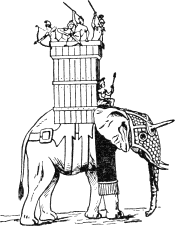
\includegraphics[width=0.3\linewidth]{./graphics/pic37.png}
  \caption{During the early days of typography fonts were designed to emulate the looks of calligraphic texts.}
  \label{fig:marginfig1}
\end{figure}

If the image is not located in the same folder as the tex-file, you will have to specify the path relative to the tex-file. This is a source of problems for many 

\begin{verbatim}
\includegraphics{./images/filename}
\end{verbatim}


\subsection{Scaling and resizing images}

If you want the image to appear in a different size, you can specifiy the size as a parameter of the |\includegraphics|-command::

\begin{commands}[]{ex:graphics}
\cmd{\includegraphics}\oarg{width=3.9cm}\marg{filename}
\end{commands}

This will scale the image to the width of 3.9 centimeters. 

Use |\textwidth| command if you don't want to specify an absolute size but rather want the actual size to depend on the text width of the page. You can use any of the normal \tex units such as \texttt{em, pt, cm, in}:

\begin{commands}[]{ex:graphics}
\cmd{\includegraphics}\oarg{width=0.5\string\textwidth}\marg{filename}
\end{commands}

\noindent will scale the image to half of the text width. The images in the
figure below were produced by three |\includegraphics| commands. You can have as many as you like and the \tex engine will treat them the same way as text. If you a leave a space between the commands, they will be positioned vertically as they are treated as paragraphs.

\medskip

\begin{commands}[]{}
\begingroup

\centering
\includegraphics[width=0.3\textwidth]{./graphics/amato.jpg}
\includegraphics[width=0.3\textwidth]{./graphics/amato.jpg}
\includegraphics[width=0.3\textwidth]{./graphics/amato.jpg}

\endgroup

\begin{verbatim}
\begingroup

\centering
\includegraphics[width=0.3\textwidth]{./graphics/amato.jpg}
\includegraphics[width=0.3\textwidth]{./graphics/amato.jpg}
\includegraphics[width=0.3\textwidth]{./graphics/amato.jpg}

\endgroup
\end{verbatim}
\captionof{figure}{Images aligned horizontally.}
\end{commands}

The three photos were centered using the |\centering| command, within a group. The |\begingroup..\endgroup| is necessary to limit the effect of centering to
the group only, otherwise \tex would center everything from this point onwards.

\subsection{Controlling the aspect ratio}

You can control the picture aspect ratio by using the command:

\begin{docCommand}{includegraphics}{\oarg{keepaspectratio,width=3cm, height=3cm}\marg{filename}}
\end{docCommand}

If the key |keepaspectratio| is set to true then specifying 
both |width| and |height| (or |totalheight|) does not distort the figure but 
scales such that neither of the specified dimensions is exceeded.


\endinput

\medskip
\begin{commands}[]{}
\begingroup

\centering
\includegraphics[width=0.3\textwidth, height=5cm]{./images/amato.jpg}
\includegraphics[keepaspectratio=true,width=4cm, height=5cm]{./images/amato.jpg}
\includegraphics[width=3cm]{./images/amato.jpg}

\endgroup

\begin{verbatim}
\begingroup

\centering
\includegraphics[width=0.3\textwidth, height=5cm]{amato}
\includegraphics[keepaspectratio=true,width=4cm, height=5cm]{amato}
\includegraphics[width=3cm]{amato}

\endgroup

\end{verbatim}
\captionof{figure}{Controlling the aspect ratio.}
\end{commands}

This can be very useful if you have images shown side by side with different
aspect ratios. 


\subsection{Paths and file types}

For larger projects you will probably find it more convenient to have 
images in different folders. You can specify default paths using:


\begin{docCommand}{graphicspath} {\marg{dir-list}} {}
\end{docCommand}

This optional declaration may be used to specify a list of directories in which to
search for graphics files. The format is the same as for the \latexe primitive
|\input@path|. A list of directories, each in a \{\} group (even if there is only one
in the list). For example:

\begin{dispListing}
\graphicspath{{eps}{tiff}}}
\end{disListing}

The default image formats can be declared using:

\begin{docCommand}{DeclareGraphicsExtensions}{ \marg{png, jpg, eps, jpeg}}{}
\end{docCommand}

This specifies the behaviour of the system when no file extension is specified in 
the argument to |\includegraphics|. \texttt{\{ext-list\}} should be a comma separated 
list of file extensions. (White space is ignored between the entries.) A file name
is produced by appending one extension from the list. If a file is found, the
system acts as if that extension had been specified. If not, the next extension
in \texttt{ext-list} is tried.



\subsection{The figure environment}

You use the figure-environment to let your image appear in a \emph{floating} environment, that is \latex will place it at the right position of a page and even on the next page:

\begin{teX}
\begin{figure}
  \includegraphics{filename.jpg}
  \caption{title of your figure}
  \label{labelname}
\end{figure}
\end{teX}

Here |\caption{...}| defines the title of the figure which will appear beneath the figure. |\label{..}| defines the label which can be used inside the document in order to insert references to the figure:

The figure

|\ref{labelname} on page \pageref{labelname} ..|

The|\label-command| inside the |\figure|-envirnonment hast to appear just after the|\caption|-command.
placing figures

If figures reside inside a |\figure|-environment, this will cause LaTeX to choose the actual location of the figure inside the document. There are different parameters for the placement strategy:

\begin{description}
\item[h (here)] Try to place the figure just where the command is located.

\item [t (top)] Try to place the figure at the top of the page.

\item[b (bottom)] Try to place the figure at the bottom of the page.

\item [p (float page)] Try to place the figure on a page which contains only floating elements.
\end{description}

The order of these parameters doesn't matter since placement is always tried in the order \textbf{h, t, b, p,} if these parameters are present:

If no parameter is present, the default order is  \texttt{[tbp]}.


The command for a figure-environment might for example look like this:

\begin{teX}
\begin{figure}[htbp]
...
\end{figure}
\end{teX}



\subsection{List of figures}
\index{figures!Table of figures}
A table of figures is inserted (where you place the command) using the command


\begin{teX}
   \listoffigures
\end{teX}

The caption given in the \cmd{caption} command is also used in the list of figures. 
If you want to use different captions, you may add a parameter to the |\caption| command:
|\caption[caption for listoffigures]{caption inside the document}|


\subsection{Figures with a border}

Although drawing frames around tables should be discouraged, if you find the need
to draw them there are  two possible ways to achieve it: either only the figure itself is bordered or there is a border around the figure and its caption. You place a border around the figure using the \cmd{\fbox} command or the \cmd{\framebox}.

\emphasis{fbox,minipage}
\begin{teX}
\begin{figure}[htbp]
  \centering
  \fbox{%
    \includegraphics{filename}%
  }%
  \caption{caption}
  \label{Labelname}
\end{figure}
\end{teX}

Placing a border around the figure and its title is a little more tricky: You need to place the figure and the title in a |\minipage| environment which is bordered again with the |\fbox| command:

\begin{figure}[htbp]
\centering
  \fbox{
    \begin{minipage}{.95\linewidth}
      \mbox{}%
      \centering
      
      \includegraphics[width=.9\linewidth]{./images/asia.jpg}%
      \caption{How to place a border around an image. }%
      \label{labelname}%
    \end{minipage}}
 
\begin{verbatim}
\begin{figure}[htbp]
  \centering
    \begin{minipage}{width=.8\linewidth}
     \centering
     
      \includegraphics[.9\linewidth]{filename}
      \caption{caption}
      \label{labelname}
    \end{minipage}
 \end{figure}
\end{verbatim}

\end{figure}



Unfortunately the width of the border cannot be determined automatically. It has to be specified as a parameter of the |\minipage| environment. However, you may be bale to develop a macro to do this,  based on the ImageSize routines we developed in section.


\section{Complex Layouts}
\label{looting}
In reality most professionally typeset books will have their own style for image pages. In Figure~\ref{complex}
three images are set in a non-symmetrical layout. This type of setting is difficult to automate and manual intervention is possible.

This layout will require four minipages. Two for the top figure (one for the image and one for the caption) and two for the two bottom figures. The rightmost bottom figure will have to be put in a zero height box to let it overflow to the top. The figure has been reproduced from an Oriental Institute publication \emph{Catastrophe! The Looting and Destruction of Iraq’s Past} \cite{looting}. The book is interesting both for its contents as well as its simple but effective typography and appropriate for the topic. The volume has been pblished in conjuction with the exhibition titled as the name of the book, that described the loss of Iraq’s archaeological past to looters and to the war. 

\begin{figure}[p]
\centering
\includegraphics[height=0.8\textheight]{oriental}
\addcredit{Oriental Institute}
\caption{More complex layouts. \emph{Copyright the Oriental Institute of the University of Chicago.}}
\label{complex}
\end{figure}

The style is reproduced in a \pkgname{phd} template (style 56) and both code and details can be found in the relevant pages.





\section{Side by side figures}

You might want to place to figures side by side but to use only one caption. This is achieved by placing both figures in its own |\minipage| which reside in the same |\figure|.

if only one |\caption| command is used, both figures will have a common title:

\medskip
\begin{verbatim}
\begin{figure}[htbp]
  \centering
  \begin{minipage}[b]{5 cm}
    \includegraphics{filename 1}  
  \end{minipage}
  \begin{minipage}[b]{5 cm}
    \includegraphics{filename 2}  
  \end{minipage}
  \caption{common caption}
  \label{Labelname}
\end{figure}
\end{verbatim}
\medskip

The first parameter of the |\minipage| environment determines how both graphics are aligned to each other. b (bottom) aligns the bottom borders of the figures, \textbf{t} (top) aligns the top borders and \textbf{c} aligns the centers.

If you want distinct titles for the two figures you will only have to supply a |\caption| command for both |\minipage|environments:

\begin{teX}
\begin{figure}[htbp]
  \centering
  \begin{minipage}[b]{5 cm}
    \includegraphics{filename 1} 
    \caption{caption 1}
    \label{labelname 1}
  \end{minipage}
  \begin{minipage}[b]{5 cm}
    \includegraphics{filename 2}  
    \caption{caption 2}
    \label{labelname 2}
  \end{minipage}
\end{figure}
\end{teX}


If you want to have subfigures with distinct caption, you use the |\subfig| package:


You can put as many figures as you like on a page, but a word of warning, you may need to make some manual adjustments before you get it right. The package provides support for the manipulation and reference of small or ‘sub’ floats within a single floating (e.g., figure or table) environment1 It is convenient to use this
package when your sub-floats are to be separately captioned, referenced, or when such
sub-captions are to be included on a List-of-Floats page.

The package is a replacement for the subfigure package, from which it was derived.
However, the new subfig package is not completely backward compatible.
Therefore, a new name was called for. The newer package is smaller and easier to use
than the older package, however, it now uses the following additional packages, 
caption (required), 
everysel (optional), 
keyval (required), 
ragged2e (optional).

It will work without the \pkgname{ragged2e} and \pkgname{everysel} packages if you do not use the following
justification options: ‘Center’, ‘RaggedRight’ and ‘RaggedLeft’. The other justification
options ‘center’, ‘raggedright’ and ‘raggedleft’ will work without the above two packages. If the ragged2e package is present, than the caption package will load it and it
will, in turn, load the everysel package. This happens whether or not you will be using
the justification options that require it. If it cannot find the ragged2e package, than the
caption package will print a message that ‘RaggedRight’, etc. will not be available.


\begin{figure}[htb]
\includegraphics[height=5cm]{dotty}
\includegraphics[height=5cm]{bette}
\includegraphics[height=5cm]{dotty}
\end{figure}

 A low bottle-shaped vase, of yellowish ware, with flaring rim and somewhat flattened body. Height, 5 inches; width 5 inches. \ref{fig:one}

A well-made bottle shaped vase, with low neck and globular body, somewhat conical above. Color dark brownish. 7½ inches in height. Shown in \ref{fig:two}


\begin{figure}
  \centering
  \includegraphics[width=0.7\linewidth]{./graphics/fig175.jpg}
   \centerline{From the tomb of a Pull\= arius.}
  \label{fig:marginfig1}
\end{figure}

The above figure is an effigy vase of the dark ware. The body is globular. A kneeling human figure forms the neck. The mouth of the vessel occurs at the back of the head—a rule in this class of vessels. Is is finely made and symmetrical. 9¾ inches high and 7 inches in diameter. being larger than the above two it is preferable to scale it to give the reader an indication. Based on the figure width, you may also need to adjust the distance between the figures to ensure that the whitespace is just about right. For screen reading this can be increased and for printed works you may wish to make it less.



\section{The wrapfig package}


\captionsetup[wrapfigure]{margin=10pt,font=small,labelfont=bf, name=Fig.} % [wrapfigure]{name=Fig.}


Donald Arseneau has created the \pkg{wrapfig} package\footfullcite{wrapfig} to allow people to place figures or
tables at the side of a page and wrap text around them. The package provides the
environments \docAuxEnv{wrapfigure} and \docAuxEnv{wraptable}. Both environments have two required and
two optional arguments. You can see an example that uses the package to wrap a picture into such a paragraph of text.

\begin{figure}[htbp]
   \includegraphics[width=\linewidth]{./graphics/cyprus.jpg} 
   \caption{Cyprian limestone group of Phoenician dancers, about 6½ in. high. There is a somewhat similar group, also from Cyprus, in the British Museum. The dress, a hooded cowl, appears to be of great antiquity.}
\end{figure}

\begin{wrapfigure}[20]{l}{3.8cm}
\centering\small
\includegraphics[width=\linewidth]{./graphics/egyptdance.jpg}  
\caption{The hieroglyphics describe the dance.}
\end{wrapfigure}
Amongst the earliest representations that are comprehensible, we have certain Egyptian paintings, and some of these exhibit postures that evidently had even then a settled meaning, and were a phrase in the sentences of the art. Not only were they settled at such an early period (B.C. 3000, fig. 1) but they appear to have been accepted and handed down to succeeding generations (fig. 2), and what is remarkable in some countries, even to our own times. The accompanying illustrations from Egypt and Greece exhibit what was evidently a traditional attitude. The hand-in-hand dance is another of these.

The earliest accompaniments to dancing appear to have been the clapping of hands, the pipes,[1] the guitar, the tambourine, the castanets, the cymbals, the tambour, and sometimes in the street, the drum.

The following account of Egyptian dancing is from Sir Gardiner Wilkinson's "Ancient Egypt"[2]:—
\begin{figure}
   \includegraphics[width=0.3\linewidth]{./graphics/lotus.jpg} 
   \caption{Cyprian limestone group of Phoenician dancers, about 6½ in. high. There is a somewhat similar group, also from Cyprus, in the British Museum. The dress, a hooded cowl, appears to be of great antiquity.}
\end{figure}
"The dance consisted mostly of a succession of figures, in which the performers endeavoured to exhibit a great variety of gesture. Men and women danced at the same time, or in separate parties, but the latter were generally preferred for their superior grace and elegance. Some danced to slow airs, adapted to the style of their movement; the attitudes they assumed frequently partook of a grace not unworthy of the Greeks; and some credit is due to the skill of the artist who represented the subject, which excites additional interest from its being in one of the oldest tombs of Thebes (B.C. 1450, Amenophis II.). Others preferred a lively step, regulated by an appropriate tune; and men sometimes danced with great spirit, bounding from the ground, more in the manner of Europeans than of Eastern people. On these occasions the music was not always composed of many instruments, and here we find only the cylindrical maces and a woman snapping her fingers in the time, in lieu of cymbals or castanets.

\begin{figure}
   \includegraphics[width=0.3\linewidth]{./graphics/patera.jpg} 
   \caption{Cyprian limestone group of Phoenician dancers, about 6½ in. high. There is a somewhat similar group, also from Cyprus, in the British Museum. The dress, a hooded cowl, appears to be of great antiquity.}
\end{figure}

"Graceful attitudes and gesticulations were the general style of their dance, but, as in all other countries, the taste of the performance varied according to the rank of the person by whom they were employed, or their own skill, and the dance at the house of a priest differed from that among the uncouth peasantry, etc.

"It was not customary for the upper orders of Egyptians to indulge in this amusement, either in public or private assemblies, and none appear to have practised it but the lower ranks of society, and those who gained their livelihood by attending festive meetings.

"Many of these postures resembled those of the modern ballet, and the pirouette delighted an Egyptian party 3,500 years ago.
\medskip

The wrapped figure is positioned using the \texttt{wrapfigure} environment, as shown below:

\begin{teX}
\begin{wrapfigure}[nlines]{placement}[overhang ]{width }
   \includegraphics[width=3.8cm]{./graphics/egyptdance} 
   \caption{The hieroglyphics describe the dance.}
\end{wrapfigure}
\end{teX}

The parameter |nlines|  is the number of narrow lines, and placement is one of r, l, i, o, R, L, I, or
O for right, le, inside, and outside, respectively. The uppercase placement specifiers
differ from their lowercase counterparts in that they force \latex to put the float \emph{here},
whereas the lowercase placement specifiers just give a hint to \latex to place them
\texttt{here}. The \meta{width} argument is the width of the figure or table that appears in the body
of the environment. Finally, \texttt{overhang} tells \latex how much the figure should hang out
into the margin of the page. Here is how one may create dangerous paragraphs bends!

The |wrapfig| package is compatible with the |caption| package. You can set the caption parameters using:---

\begin{teX}
\captionsetup[wrapfigure]{<options>}
\end{teX}

If you are probably wondering how |wrapfig| achieves this, you should read the package code. It basically uses \refCom{everypar}, and hence the limitations with |\par|. Here is an extract from the class.

\begin{teX}

% Subvert \everypar to float fig and do wrapping.  
% Also for non-float.
\def\WF@startfloating{%
 \WF@everypar\expandafter{\the\everypar}\let\everypar\WF@everypar
 \WF@@everypar{\ifvoid\WF@box\else\WF@floathand\fi \the\everypar
 \WF@wraphand
}}
\end{teX}

Moving now to a more scientific example that the previous ones, we will place two figures
one on top of each other and give them individual, sub-captions as shown in \ref{fig:honey}.
 
\captionsetup[figure]{margin=10pt,font=small,labelfont=bf,format=hang}%

\begin{figure}[htbp]
\centering
  \begin{subfigure}[b]{0.5\textwidth}
  \includegraphics[width=\linewidth]{./graphics/honey.png}
  \caption{Taylor instability in the surface of the honey in an inverted honey jar.}\label{fig:honey}
    \hspace{1cm}
  \end{subfigure}

  \begin{subfigure}[b]{0.9\textwidth}
     \centering
     \includegraphics[width=9cm]{./graphics/honeydrops.png}
     \caption{Taylor instability in the interface of the water condensing on the underside of a small water pipe.}
  \end{subfigure}  
  \caption{Two examples of Taylor instabilities that are commonly found.}%
    \label{fig:Athird}%
\end{figure}

The figures are from \textit{A Heat Transfer Textbook}, by J.H.Lienhard, which incidentally was typeset using
\tex . It is a McGrawHill publication. 

\begin{teX}
\begin{figure}[htbp]
    \captionsetup[figure]{margin=10pt}%
    \subfloat[Taylor instability...]
     {{\includegraphics[width=8cm]{./graphics/honey}}}
    \hspace{1cm}
     \subfloat[Taylor instability in the...]%
      {\includegraphics[width=9cm]{./graphics/honeydrops}}  
     \\[-10pt]
   \caption{Taylor instability in...}%
    \label{fig:Afirst}%
    \caption{Two examples of... }%
    \label{fig:honey}%
\end{figure}
\end{teX}


The text can have more than one paragraph. It is also possible to include figures
generated by |TikZ/pgf|, as shown in the next example, drawn from real code
in the book.


%\begin{wrapfigure}[14]{l}{3.0cm}
%\pgfplotsset{width=5.0cm,compat=1.3}
%\begin{tikzpicture}
%\begin{axis}[minor y tick num=4, 
%minor x tick num=4, 
%xmin=0,xmax=300,
%ymin=0,ymax=60,
%xlabel=\textsf{liquidus ($l/s$)},
%ylabel=\textsf{capitis ($m$)}, 
%ytick={0,15,30,45,60,75},
%xtick={0,100,200,300}
%]
%\addplot[color=blue,mark=x, smooth] coordinates {
%(0,44)
%(50,43)
%(100,42)
%(150,40)
%(200,33)
%(220,29)
%};
%
%\end{axis}
%\end{tikzpicture}
%\captionof{figure}{Pump headum and flowm}
%%\end{wrapfigure}



\begin{figure}[htp]
\centering

\captionsetup{name=Photo., labelsep=period, format=plain}%
   \begin{minipage}[t]{0.48\textwidth}
      \includegraphics[width=\textwidth]{./graphics/movingup.jpg}%
      \vskip1pt\addcredit{U.S. DoD.}%
     \caption{The effects of the credit going past the edge of the figure. This can be corrected by adding a minipage to hold both commands. }
\end{minipage}\hfill\hfill
\begin{minipage}[t]{0.48\textwidth}
      \includegraphics[width=\textwidth]{./graphics/survivors.jpg}%
      \addcredit{U.S. DoD.%
    {\footnotesize Marines awaiting resting before moving on to Japan. }}%
    \flushleft
    \caption[Adding a credit to an image.]{The effects of the credit going past the edge of the figure. This can be corrected by adding a minipage to hold both commands. }
    
\end{minipage}
% \begin{minipage}[t]{0.48\textwidth}
%      \includegraphics[width=\textwidth]{./graphics/img009.jpg}%
%      \addcredit{U.S. DoD.}%
%     \caption{Engineer Construction Troops in Liberia, July 1942.}
%\end{minipage}\hfill\hfill
%\begin{minipage}[t]{0.48\textwidth}
%      \includegraphics[width=\textwidth]{./graphics/survivors.jpg}%
%      \addcredit{U.S. DoD.}%
%     \caption{The effects of the credit going past the edge of the figure. This can be corrected by adding a minipage to hold both commands. }
%\end{minipage}
% \begin{minipage}[t]{0.48\textwidth}
%      \includegraphics[width=\textwidth]{./graphics/img126.jpg}%
%      \addcredit{U.S. DoD.}%
%     \caption{Marine Reinforcements.
%A light machine gun squad of 3d Battalion, 1st Marines, arrives during the battle for ``Boulder City.'' }
%\end{minipage}\hfill\hfill
%\begin{minipage}[t]{0.48\textwidth}
%      \includegraphics[width=\textwidth]{./graphics/img124.jpg}%
%      \addcredit{U.S. DoD.}%
%     \caption{Brothers Under the Skin, inductees at Fort Sam Houston, Texas, 1953. }
%\end{minipage}
\par
\end{figure}


Armed with all these packages you can help the Gutenburg organization to transcribe
some of the old books that they have online. 









  
\chapter{Key Value Interfaces}

The key value system greatly simplifies the \tex interface for authors. As \cite{joseph2009} wrote this ease of use was not transferred into settting up key-value systems for authors of pre-packaged \tex code. This Chapter and the one that follows that focus specifically on the \pkg{pgfkeys} package provides an overview and describes some of the more difficult areas. The TUGboat article referenced earlier and written by Joseph Wright \textit{et.al} has an excellent introduction to the available packages and some longer examples for comparison. Chapter~\ref{ch:l3keys}
\nameref{ch:l3keys} discusses the |expl3| key-value functions.

\section{keyval}

The \pkg{keyval} written by David Carlisle is still widely used by package authors to provide the means for users to easily specify numerous optional arguments for macros \cite{keyval}. The main advantages of using keyval are that  (1) the number of optional arguments is no longer limited to 9 and that (2) the arguments are named, and hence there is less chance of confusion about the syntax of a macro.

\section{xkeyval}

A more recent package, \pkg{xkeyval} provides improvements for programming keys and  also
provides a more advanced interface for the namespacing of keys and families.
Before you start experimenting with the xkeyval package, I suggest that you load the package \pkg{xkview}. This is part of the \ctan{xkeyval}  bundle and can help you to view key value parameters in various ways. The \pkg{xkeyval} package was developed by Hendri Adriaens and Uwe Kern\footcite{xkeyval}. This package is an extension of the well-known |keyval| package. The package provides more flexible commands and syntax enhancements as well as newer option processing mechanism.

The main change of the |xkeyval| package is that it provides a means to namespace the keys, which all have the form |\KV@family@keyname|, where the KV is a literal prefix to avoid collisions. They take one argument to handle user input.

The main commands of the package are the same as those of keyval. 

\begin{texexample}{xkeyval }{}
\makeatletter
\define@key{phd}{pi}{\setlength{\parindent}{#1}}
\setkeys{phd}{pi=50pt}
\makeatother
\lorem\par
\setkeys{phd}{pi=0pt}
\lorem\par
\end{texexample}

Defining a default key, i.e., a key that can be used as |indent| or |indent=30pt| will stretch your memory, as it has an optional parameter as its third argument. 

\begin{verbatim}
\define@key{family}{key}[none]{The input is: #1}
\end{verbatim}

\begin{texexample}{xkeyval }{}
\makeatletter

\define@key{phd}{pi}[30pt]{\setlength{\parindent}{#1}}

\setkeys{phd}{pi}

\lorem

or \setkeys{phd}{pi=0pt}

\lorem
\makeatother
\end{texexample}

\section{Ordinary Keys}
\makeatletter
\define@key{phd}{pi}[1em]{\setlength{\parindent}{#1}}
\makeatother


Ordinary keys are keys that have values such as \texttt{animal=elephant} and your macro can be called like \texttt{animals[animal=elephant]\{14\}}.

   

\section{Keys and values in package options}

First of all, the package supplies macros to declare class or package options, execute them and process
them. The macros are available under the usual
\latex names, but all with the suffix \textbf{X}, namely

\begin{docCommand}{DeclareOptionX}{}
\begin{docCommand}{DeclareOptionX*}{}
\begin{docCommand}{ExecuteOptionsX}{}
\begin{docCommand}{ProcessOptionsX}{}
These commands allow the user to assign a value to
an option just like when using |\setkeys|. The first
macro is based on |\define@key| and the final two
are based on |\setkeys|. Supposing that a package
|mypack| is set up with these commands, a user could
for instance do
\end{docCommand}
\end{docCommand}
\end{docCommand}
\end{docCommand}

\begin{verbatim}
\usepackage[textcolor=red,font=times]{mypack}
\end{verbatim}

These |xkeyval|macros are fully compatible with the \latex option conventions. They will allow packages to copy global options specified in the |\documentclass| command, to pass options to other classes or packages and to update the list of unused global options that will be displayed by \latex in the log file. 


\section{kvoptions}

Another package \pkg{kvoptions} by Heiko Oberdiek is used extensively in the large suite of packages
developed by Heiko \footcite{kvoptions}. The package originally formed part of the \pkg{hyperref} and later branched into an independent package. The package provides a number of additional commands to those found in the \latexe kernel and a comparison of the commands is shown in the table below. 

It is a good alternative that can be used for single topic package writing. An important feature of the package is its ability to process options both globally as well as locally avoiding conflicts when options are specified both globally as well as locally. Heiko provides an example from his bookmark package \footcite{bookmark}, which provides the option \option{open}
that specifies whether the bookmarks are opened or closed initially. Its values are
true or false. Since KOMA-Script version 3.00 the KOMA classes also introduces
option open with values right and any and a complete different meaning.
Such conflicts can be resolved by marking all or part of options as local by
\refCmd{DeclareLocalOption} or \refCmd{DeclareLocalOptions}. Then the packages ignores
global occurences of these options


\endinput
\chapter{Managing Keys with PGF}
\section{PGF keys}
\label{ch:pgfkeys}

This chapter describes the package |pgfkeys|. It is loaded
automatically by both \pgfname\ and \tikzname.


  This package can be used independently of \pgfname. Note that no
  other package of \pgfname\ needs to be loaded (so neither the
  emulation layer nor the system layer is needed). The Con\TeX t
  abbreviation is |pgfkey| if |pgfmod| is not loaded.
  
\long\def\uwavestory{A Dialogue between the Landlady, and Susan the Chambermaid, proper to be read by all Innkeepers, and their Servants; with the Arrival, and affable Behaviour of a beautiful young Lady; which may teach Persons of Condition how they may acquire the Love of the whole World.}
         
\def\fontstore{}
\def\fractionlinewidth{\linewidth}

\cxset{paragraph style/uwave/.code=\wavelast{#1},
       paragraph style/uwave/font-weight/.store in=\fontstore{#1}, 
       paragraph style/uwave/linewidth/.code=\fractionlinewidth{#1},
       }
       
 \cxset{paragraph style/uwave/font-weight=\itshape,
      % paragraph style/uwave/linewidth={15cm},
       }      
       
\def\wavelast#1{%
       \bgroup
       \hbox to \linewidth{\hfill\vbox{%
       \fontstore
       \hsize=0.8\linewidth
       \hyphenpenalty=100
       \setbox0=\vbox{\noindent\centering #1}%
       \setbox1=\vbox{%
            \unvbox0
            \setbox2=\lastbox
            \centerline{\uwave{\unhbox2}}%
       }%
       \unvbox1
       }\hfill}%
       \bigskip
      \egroup
  }

\begin{texexample}{wavelast}{}
\bgroup
\cxset{paragraph style/uwave/font-weight=\itshape,
      % paragraph style/uwave/linewidth={15cm},
       }
\begin{center}       

 \wavelast{
A Dialogue between the Landlady, and Susan the Chambermaid, proper to be read by all Innkeepers, and their Servants; with the Arrival, and affable Behaviour of a beautiful young Lady; which may teach Persons of Condition how they may acquire the Love of the whole World.}

\end{center}
\egroup
\end{texexample}

\emphasis{uwave}
\begin{teXXX}
\def\wavelast#1{%
       \bgroup
       
       \setbox0=\vbox{\fontstore\noindent #1}%
       \setbox1=\vbox{%
            \unvbox0
            \setbox2=\lastbox
            \hbox to 10cm{\hfill\uwave{\unhbox2}\hfill}(*@\label{lin:uwave}@*)%
       }%
       \unvbox1
      \egroup
  }%
\end{teXXX}



Consider the number of variables involved in such a paragraph. How can we abstract the code to make it more general? We can have settings for colors, width, hyphenation, font related commands etc. \pgfname\ keys can be used to provide a dictionary.



 \cxset{paragraph style/uwave/font-weight=\bfseries,
        paragraph style/uwave=\uwavestory}

\medskip

 \cxset{paragraph style/uwave/font-weight=\itshape\bfseries,
        paragraph style/uwave=\aliceii}       




\section{Introduction}

\subsection{Comparison to Other Packages}

The |pgfkeys| package defines a key--value management system that is in
some sense similar to the more light-weight |keyval| system and the
improved |xkeyval| system. However, |pgfkeys| uses a slightly
different philosophy than these systems and it will coexist peacefully
with both of them. Its power and flexibility are evident in the |pgf|
and |tikz| packages and to an extend our own |phd| system.

The main differences between |pgfkeys| and |xkeyval| are the
following:

\begin{itemize}
\item |pgfkeys| organizes keys in a tree, while |keyval| and |xkeyval|
  use families. In |pgfkeys| the families correspond to the root
  entries of the key tree.
\item For efficiency reasons, |pgfkeys| does not directly support
  setting keys drawn from multiple families as |xkeyval| does. This
  can be emulated if necessary, but it will be slower than |xkeyval|'s
  native support.
\item |pgfkeys| has no save-stack impact (you will have to read the
  \TeX Book very carefully to appreciate this).
\item |pgfkeys| is slightly slower than |keyval|, but not much.
\item |pgfkeys| supports styles. This means that keys can just stand
  for other keys (which can stand for other keys in turn or which can
  also just execute some code). \tikzname\ uses this mechanism heavily.
\item |pgfkeys| supports multi-argument key code. This can, however,
  be emulated in |keyval|.
\item |pgfkeys| supports handlers. These are call-backs that are
  called when a key is not known. They are very flexible, in fact even
  defining keys in different ways is handled by, well, handlers.
\end{itemize}

The \pgfname can be used for complicated and multi-value cases. The fact that it is
more capable than the rest does not in itself make it slower. 

\section{Technical}

The package uses \cs{csname} to craete the names of macros and token registers to store the values. For example to
store a length in a key |/test/length| it does the following:

\begin{texexample}{pgfkeyssetvalue}{ex:setexpl}
\pgfkeyssetvalue{/test/length}{2cm-3cm}
\makeatletter
\the\pgfkeys@temptoks

\csname pgfk@/test/length\endcsname
\makeatother
\end{texexample}

Essentially we defined a macro |pgfk@/test/length| with its replacement text being |2cm-3cm|. The definition
of \docAuxCommand{pgfkeyssetvalue} given by:

\begin{teXXX}
\long\def\pgfkeyssetvalue#1#2{%
  \pgfkeys@temptoks{#2}
  \expandafter
    \edef\csname pgfk@#1\endcsname{\the\pgfkeys@temptoks}%
}
\end{teXXX}

The code above just stored a value. If the path ends in |.@cmd| it will set up things so the |key/.@cmd| contains a 
a macro that takes one parameter and has |#2| as its code.

\begin{teXXX}
\long\def\pgfkeysdef#1#2{%
  \long\def\pgfkeys@temp##1\pgfeov{#2}%
  \pgfkeyslet{#1/.@cmd}{\pgfkeys@temp}%
  \pgfkeyssetvalue{#1/.@body}{#2}%
}

\long\def\pgfkeysedef#1#2{%
  \long\edef\pgfkeys@temp##1\pgfeov{#2}%
  \pgfkeyslet{#1/.@cmd}{\pgfkeys@temp}%
  \pgfkeyssetvalue{#1/.@body}{#2}%
}
\end{teXXX}


\begin{texexample}{Defining keys for code}{ex:keycode}

\def\city#1{\expandafter\def\csname#1\endcsname{#1}}

\pgfkeysdef{/test/cities}{\city{#1}}

\pgfkeys{/test/cities=Rome}
\pgfkeys{/test/cities=Paris}

\Rome, \Paris



\end{texexample}




\subsection{Getting started}

The following quick guide to \pgfname's key mechanism only treats the
most commonly used features. For an in-depth discussion of what is
going on, please consult the \pgfname\ manual.

Keys are organized in a large tree that is similar to the Unix
file tree. A typical key might be, say, \lstinline{/tikz/coordinate system/x}
or just |/x|. Again as in Unix, when you specify keys you can provide
the complete path of the key, but you usually just provide the name of
the key (corresponding to the file name without any path) and the path
is added automatically.

Typically (but not necessarily) some code is associated with a key. To
execute this code, you use the |\pgfkeys| command. This command takes
a list of so-called key--value pairs. Each pair is of the form
\meta{key}|=|\meta{value}. For each pair the |\pgfkeys| command will
execute the code stored for the \meta{key} with its parameter set to
\meta{value}.

Here is a typical example of how the |\pgfkeys| command is used:
\begin{codeexample}[code only]
\pgfkeys{/my key=hallo,/your keys/main key=something\strange,
         key name without path=something else}
\end{codeexample}

Now, to set the code that is stored in a key you do not need to learn
a new command. Rather, the |\pgfkeys| command can also be used to set
the code of a key. This is done using so-called \emph{handlers}. They
look like keys whose names look like ``hidden files in Unix'' since
they start with a dot. The handler for setting the code of a key is
appropriately called |.code| and it is used as follows:
\begin{codeexample}[]
\pgfkeys{/my key/.code=The value is '#1'.}
\pgfkeys{/my key=hi!}
\end{codeexample}
As you can see, in the first line we defined the code for the key
|/my key|. In the second line we executed this code with the parameter
set to |hi!|.

There are numerous handlers for defining a key. For instance, we can
also define a key whose value actually consists of more than one
parameter. 
\begin{codeexample}[]
\pgfkeys{/my key/.code 2 args=The values are '#1' and '#2'.}
\pgfkeys{/my key={a1}{a2}}
\end{codeexample}

We often want to have keys where the code is called with some default
value if the user does not provide a value. Not surprisingly, this is
also done using a handler, this time called |.default|.
\begin{codeexample}[]
\pgfkeys{/my key/.code=(#1)}
\pgfkeys{/my key/.default=hello}
\pgfkeys{/my key=hallo,/my key}
\end{codeexample}

The other way round, it is also possible to specify that a value
\emph{must} be specified, using a handler called
|.value required|. Finally, you can also require that no value
\emph{may} be specified using |.value forbidden|.

All keys for a package like, say, \tikzname\ start with the path
|/tikz|. We obviously do not like to write this path down every
time we use a key (so we do not have to write things like
|\draw[/tikz/line width=1cm]|). What we need is to somehow ``change
the default path to a specific location.'' This is done using the
handler |.cd| (for ``change directory''). Once this handler has been
used on a key, all subsequent keys {\itshape in the current call of
  |\pgfkeys| only} are automatically prefixed with this path, if
necessary.

Here is an example:
\begin{codeexample}[code only]
\pgfkeys{/tikz/.cd,line width=1cm,line cap=round}
\end{codeexample}
This makes it easy to define commands like |\tikzset|, which could be
defined as follows (the actual definition is a bit faster, but the
effect is the same):
\begin{codeexample}[code only]
\def\tikzset#1{\pgfkeys{/tikz/.cd,#1}}
\end{codeexample}

When a key is handled, instead of executing some code, the key can
also cause further keys to be executed. Such keys will be called
\emph{styles}. A style is, in essence, just a key list that should be
executed whenever the style is executed. Here is an example:
\begin{codeexample}[]
\pgfkeys{/a/.code=(a:#1)}
\pgfkeys{/b/.code=(b:#1)}
\pgfkeys{/my style/.style={/a=foo,/b=bar,/a=#1}}
\pgfkeys{/my style=wow}
\end{codeexample}
As the above example shows, style can also be parametrized, just like
the normal code keys.

Printing a phd key 
\begin{texexample}{Printing a Key}{ex:key}
\pgfkeys{/phd/test/.code=(Test),}
\pgfkeys{/phd/.style =/phd/.cd,
         phd, chapter name,
         }
\expandafter\meaning\expandafter\pgfkeysvalueof{/phd/chapter font-family}   
\makeatletter
\csname pgfkey@store\endcsname {test}
\makeatother      
\end{texexample}


As a typical use of styles, suppose we wish to setup the key |/tikz|
so that it will change the default path to |/tikz|. This can be
achieved as follows:
\begin{codeexample}[code only]
\pgfkeys{/tikz/.style=/tikz/.cd}
\pgfkeys{tikz,line width=1cm,draw=red}
\end{codeexample}

Note that when |\pgfkeys| is executed, the default path is set
to~|/|. This means that the first |tikz| will be completed to
|/tikz|. Then |/tikz| is a style and, thus, replaced by |/tikz/.cd|,
which changes the default path to |/tikz|. Thus, the |line width| is
correctly prefixed with |/tikz|.

\subsection{The Key Tree}

The |pgfkeys| package organizes keys in a so-called \emph{key
  tree}. This tree will be familiar to anyone who has used a Unix
operating system: A key is addressed by a path, which consists of
different parts separated by slashes. A typical key might be
|/tikz/line width| or just |/tikz| or something more complicated like
|/tikz/cs/x/.store in|.

Let us fix some further terminology: Given a key like |/a/b/c|, we
call the part leading up the last slash (|/a/b|) the \emph{path} of
the key. We call everything after the last slash (|c|) the \emph{name}
of the key (in a file system this would be the file name). 

We do not always wish to specify keys completely. Instead, we usually
specify only part of a key (typically only the name) and the
\emph{default path} is then added to the key at the front. So, when
the default path is |/tikz| and you 
refer to the (partial) key |line width|, the actual key that is used
is |/tikz/line width|. There is a simple rule for deciding whether a
key is a partial key or a full key: If it starts with a slash, then it
is a full key and it is not modified; if it does not start with
a slash, then the default path is automatically prefixed.

Note that the default path is not the same as a search path. In
particular, the default path is just a single path. When a partial key
is given, only this single default path is prefixed; |pgfkeys| does
not try to lookup the key in different parts of a search path. It is,
however, possible to emulate search paths, but a much more
complicated mechanism must be used.

When you set keys (to be explained in a moment), you can freely mix
partial and full keys and you can change the default path. This makes
it possible to temporarily use keys from another part of the key tree
(this turns out to be a very useful feature).

Each key (may) store some \emph{tokens} and there exist commands,
described below, for setting, getting, and changing the tokens stored
in a key. However, you will only very seldom use these commands
directly. Rather, the standard way of using keys is the |\pgfkeys|
command or some command that uses it internally like, say,
|\tikzset|. So, you may wish to skip the following commands and
continue with the next subsection.

\begin{docCommand}{pgfkeyssetvalue}{\marg{full key}\marg{token text}}{}
  Stores the \meta{token text} in the \meta{full key}. The \meta{full key}
  may not be a partial key, so no default-path-adding is done. The
  \meta{token text} can be arbitrary tokens and may even contain things
  like |#| or unbalanced \TeX-ifs.
\begin{codeexample}[]
\pgfkeyssetvalue{/my family/my key}{Hello, world!}
\pgfkeysvalueof{/my family/my key}  
\end{codeexample}

  The setting of a key is always local to the current \TeX\ group.
  
\begin{codeexample}[]
\pgfkeyssetvalue{/phd/chapteris font}{\arial}
{\pgfkeysvalueof{/phd/chapteris font}  Lorem ipsum ...}
\end{codeexample}  
\end{docCommand}




\begin{docCommand}{pgfkeyslet}{\marg{full key}\marg{macro}}
  Performs a |\let| statement so the the \meta{full key} pionts to the
  contents of \meta{macro}.
\begin{codeexample}[]
\def\helloworld{Hello, world!}
\pgfkeyslet{/my family/my key}{\helloworld}
\pgfkeysvalueof{/my family/my key}  
\end{codeexample}
  You should never let a key be equal to |\relax|. Such a key may or
  may not be indistinguishable from an undefined key.
\end{docCommand}

\begin{docCommand}{pgfkeysgetvalue}{\marg{full key}\marg{macro}}{}
  Retrieves the tokens stored in the \meta{full key} and lets
  \meta{macro} be equal to these tokens. If the key has
  not been set, the \meta{macro} will be equal to |\relax|. 
\begin{codeexample}[]
\pgfkeyssetvalue{/my family/my key}{Hello, world!}
\pgfkeysgetvalue{/my family/my key}{\helloworld}
\helloworld
\end{codeexample}
\end{docCommand}



\begin{docCommand}{pgfkeysvalueof}{\marg{full key}}
  Inserts the value stored in \meta{full key} at the current position
  into the text.

\begin{codeexample}[]
\pgfkeyssetvalue{/my family/my key}{Hello, world!}
\pgfkeysvalueof{/my family/my key}
\end{codeexample}
\end{docCommand}

%

\begin{docCommand}{pgfkeysifdefined}{\marg{full key}\marg{if}\marg{else}}{}
  Checks whether this key was previously set using either
  |\pgfkeyssetvalue| or |\pgfkeyslet|. If so, the code in \meta{if} is
  executed, otherwise the code in \meta{else}.

  This command will use e\TeX's |\ifcsname| command, if available, for
  efficiency. This means, however, that it may behave differently for
  \TeX\ and for e\TeX\ when you set keys to |\relax|. For this reason
  you should not do so. 

\begin{codeexample}[]
\pgfkeyssetvalue{/my family/my key}{Hello, world!}
\pgfkeysifdefined{/my family/my key}{yes}{no}
\end{codeexample}
\end{docCommand}



\subsection{Setting Keys}{ }

Settings keys is done using a powerful command called |\pgfkeys|. This
command takes a list of so-called \emph{key--value pairs}. These are
pairs of the form \meta{key}|=|\meta{value}. The principle idea is the
following: For each pair in the list, some \emph{action} is
taken. This action can be one of the following:

\begin{enumerate}
\item A command is executed whose argument(s) are \meta{value}. This
  command is stored in a special subkey of \meta{key}.
\item The \meta{value} is stored in the \meta{key} itself.
\item If the key's name (the part after the last slahs) is a known
  \emph{handler}, then this handler will take care of the key.
\item If the key is totally unknown, one of several possible
  \emph{unknown key handlers} is called. 
\end{enumerate}

Addtionally, if the \meta{value} is missing, a default value may or
may not be substituted. Before we plunge into all the details,
let us have a quick look at the command itself.

\begin{docCommand}{pgfkeys}{\marg{key list}}{}
  The \meta{key list} should be a list of key--value pairs, separated
  by commas. A key--value pair can have the following two forms:
  \meta{key}|=|\meta{value} or just \meta{key}. Any spaces around the
  \meta{key} or around the \meta{value} are removed. It is permissible
  to surround both the \meta{key} or the \meta{value} in curly braces,
  which are also removed. Especially putting the \meta{value} in curly
  braces needs to be done quite often, namely whenever the \meta{value}
  contains an equal-sign or a comma.

  The key--value pairs in the list are handled in the order they
  appear. How this handling is done, exactly, is described in the rest
  of this section.

  If a \meta{key} is a partial key, the current value of the default
  path is prefixed to the \meta{key} and this ``upgraded'' key is
  then used. The default path is just the root path |/| when the first
  key is handled, but it may change later on. At the end of the
  command, the default path is reset to the value it had before this
  command was executed. 
  
  Calls of this command may be nested. Thus, it is permissible to call
  |\pgfkeys| inside the code that is executed for a key. Since the
  default path is restored after a call of |\pgfkeys|, the default
  path will not change when you call |\pgfkeys| while executing code
  for a key (which is exactly what you want).
\end{docCommand}

\begin{docCommand}{pgfqkeys}{\marg{default path}\marg{key list}}{}
  This command has the same effect as |\pgfkeys{|\meta{default
      path}|/.cd,|\meta{key list}|}|, it is only marginally
  quicker. This command should not be used in user code, but rather in
  commands like |\tikzset| or |\pgfset| that get called very often.   
\end{docCommand}

\begin{docCommand}{pgfkeysalso}{\marg{key list}}{}
  This command has execatly the same effect as |\pgfkeys|, only the
  default path is not modified before or after the keys are being
  set. This command is mainly intended to be called by the code that
  is being processed for a key.
\end{docCommand}

\begin{docCommand}{pgfqkeysalso}{\marg{default path}\marg{key list}}{}{}
  This command has the same effect as |\pgfkeysalso{|\meta{default
      path}|/.cd,|\meta{key list}|}|, it is only quicker. Changing the
  default path inside a |\pgfkeyalso| is dangerous, so use with
  care. A rather safe place to call this command is at the beginning
  of a \TeX\ group.
\end{docCommand}



\subsubsection{Default Arguments} 

The arguments of the |\pgfkeys| command can either be of the form
\meta{key}|=|\meta{value} or of the form \meta{key} with the
value-part missing. In the second case, the |\pgfkeys| will try to
provide a \emph{default value} for the \meta{value}. If such a default
value is defined, it will be used as if you had written
\meta{key}|=|\meta{default value}.

In the following, the details of how default values are determined is
described; however, you should normally use the handlers |.default|
and |.value required| as described in
Section~\ref{section-default-handlers} and you can may wish to skip
the following details.

When |\pgfkeys| encounters a \meta{key} without an equal-sign, the
following happens:
\begin{enumerate}
\item The input is replaced by \meta{key}|=\pgfkeysnovalue|. In
  particular, the commands |\pgfkeys{my key}| and
  |\pgfkeys{my key=\pgfkeysnovalue}| have exactly the same effect and
  you can ``simulate'' a missing value by providing the value
  |\pgfkeysnovalue|, which is sometimes useful. 
\item If the \meta{value} is |\pgfkeysnovalue|, then it is checked
  whether the subkey \meta{key}|/.@def| exists. For instance, if you
  write |\pgfkeys{/my key}|, then it is checked whether the key
  |/my key/.@def| exists.
\item If the key \meta{key}|/.@def| exists, then the tokens stored in
  this key are used as \meta{value}.
\item If the key does not exist, then |\pgfkeysnovalue| is used as the
  \meta{value}.
\item At the end, if the \meta{value} is now equal to
  |\pgfkeysvaluerequired|, then the code  (or something fairly equivalent)
  |\pgfkeys{/errors/value required=|\meta{key}|{}}|
  is executed. Thus, by changing this key you can change the error
  message that is printed or you can handle the missing value in some
  other way.
\end{enumerate}



\subsection{Keys That Execute Commands}

\label{section-key-code}

After the transformation process described in the previous subsection,
we arrive at a key of the form \meta{key}=\meta{value}, where
\meta{key} is a full key. Different things can now happen, but always
the macro |\pgfkeyscurrentkey| will have been setup to expand to the
text of the \meta{key} that is currently being processed.

The first things that is tested is whether the key \meta{key}|/.@cmd|
exists. If this is the case, then it is assumed that this key stores
the code of a macro and this macro is executed. The argument of this
macro is \meta{value} directly followed by |\pgfeov|, which stands for
``end of value.'' The \meta{value} is not surrounded by braces. After
this code has been executed, |\pgfkeys| continues with the next key in
the \meta{key list}.

It may seem quite peculiar that the macro stored in the key
\meta{key}|/.@cmd| is not simply executed with the argument
|{|\meta{value}|}|. However, the approach taken in the |pgfkeys|
packages allows for more flexibility. For instance, assume that you
have a key that expects a \meta{value} of the form
``\meta{text}|+|\meta{more text}'' and wishes to store \meta{text} and
\meta{more text} in two different macros. This can be achieved as
follows:

\begin{texexample}{Storing values in macros}{ex:storemacro}{ }

\def\mystore#1+#2\pgfeov{\def\a{#1}\def\b{#2}}
\pgfkeyslet{/my key/.@cmd}{\mystore}
\pgfkeys{/my key=hello+world}

|\a| is \a, |\b| is \b.
\end{texexample}

Naturally, defining the code to be stored in a key in the above manner
is too awkward. A simpler approach is shown in Example~\ref{delineated}. The following commands simplify things a bit, but the
usual manner of setting up code for a key is to use one of the
handlers described in Section~\ref{section-code-handlers}.

\begin{docCommand}{pgfkeysdef}{\marg{key} \marg{code}}
  This command temporarily defines a \TeX-macro with the argument list
  |#1\pgfeov| and then lets \meta{key}|/.@cmd| be equal to this
  macro. The net effect of all this is that you have then setup code
  for the key \meta{key} so that when you write
  |\pgfkeys{|\meta{key}|=|\meta{value}|}|, then the \meta{code} is
  executed with all occurrences of |#1| in \meta{code} being replaced
  by \meta{value}. (This behaviour is quite similar to the
  |\define@key| command of |keyval| and |xkeyval|).

%\begin{codeexample}[]
%\pgfkeysdef{/my key}{#1, #1.}
%\pgfkeys{/my key=hello}
%\end{codeexample}
\end{docCommand}

\begin{docCommand}{pgfkeysedef}{\marg{key} \marg{code}}
  This command works like |\pgfkeysdef|, but it uses |\edef| rather
  than |\def| when defining the key macro. If you do not know the
  difference between the two, then you will not need this command;
  and if you know the difference, then you will know when you need this
  command.
\end{docCommand}

\begin{docCommand}{pgfkeysdeargs}{\marg{key}\marg{argument pattern}\marg{code}}{}
  This command works like |\pgfkeysdef|, but it allows you to provide
  an arbitrary \meta{argument pattern} rather than just the simple
  single argument of |\pgfkeysdef|. 
\end{docCommand}
\begin{texexample}{Delineated arguments}{delineated}{}
\pgfkeysdefargs{/my key}{#1+#2}{\def\a{#1}\def\b{#2}}
\pgfkeys{/my key=hello+world}

|\a| is \a, |\b| is \b.
\end{texexample}


\begin{docCommand}{pgfkeysedefargs}{\marg{key}\marg{argument pattern}\marg{code}}{}
  The |\edef| version of |\pgfkeysdefargs|.
\end{docCommand}


\subsection{Keys That Store Values}

Let us continue with what happens when |\pgfkeys| processes the
current key and  the subkey \meta{key}|/.@cmd| is not defined. Then
it is checked whether the \meta{key} itself exists (has been
previously assigned a value using, for instance,
|\pgfkeyssetvalue|). In this case, the tokens stored in \meta{key} are
replaced by \meta{value} and |\pgfkeys| proceeds with the next key in
the \meta{key list}. 


\subsection{Keys That Are Handled}
\label{section-key-handlers}

If neither the \meta{key} itself nor the subkey \meta{key}|/.@cmd| are
defined, then the \meta{key} cannot be processed ``all by itself.''
Rather, a \meta{handler} is needed for this key. Most of the power of
|pgfkeys| comes from the proper use of such handlers.

Recall that the \meta{key} is always a full key (if it was not
originally, it has already been upgraded at this point to a full
key). It decomposed into  two parts:

\begin{enumerate}
\item The \meta{path} of \meta{key} (everything
  before the last slash) is stored in the macro |\pgfkeyscurrentpath|.
\item The \meta{name} of \meta{key} (everything
  after the last slash) is stored in the macro |\pgfkeyscurrentname|.

  It is recommended (but not necessary) that the name of a handler
  starts with a dot (but not with |.@|), so that they are easy to
  detect for the reader.  
\end{enumerate}

(For efficiency reasons, these two macros are only setup at this point;
so when code is executed for a key in the ``usual'' manner then these
macros are not setup.)

The |\pgfkeys| command now checks whether the key
|/handlers/|\meta{name}|/.@cmd| exists. If so, it should store a command
and this command is executed exactly in the same manner as described
in Section~\ref{section-key-code}.
Thus, this code gets the \meta{value} that was originally intended for
\meta{key} as its argument, followed by |\pgfeov|.
It is the job of the handlers to so something useful with the
\meta{value}.

For an example, let us write a handler that will output the value
stored in a key to the log file. We call this handler
|.print to log|. The idea is that when someone tries to use the key
|/my key/.print to log|, then this key will not be defined and the
handler gets executed. The handler will then have access to the
path-part of the key, which is |/my key|, via the macro
|\pgfkeyscurrentpath|. It can then lookup which value is stored in
this key and print it.

\begin{codeexample}[code only]
\pgfkeysdef{/handlers/.print to log}
{%
  \pgfkeysgetvalue{\pgfkeyscurrentpath}{\temp}
  \writetolog{\temp}
}
\pgfkeyssetvalue{/my key}{Hi!}
...
\pgfkeys{/my key/.print to log}

\pgfkeys{/phd/chapter label/.font-size}

font sise
\end{codeexample}
The above code will print |Hi!| in the log, provided the macro
|\writetolog| is setup appropriately.

For a more interesting handler, let us program a handler that will
setup a key so that when the key is used some code is executed. This
code is given as \meta{value}. All the handler must do is to call
|\pgfkeysdef| for the path of the key (which misses the handler's
name) and assign the parameter value to it.

\begin{texexample}{Defining Handlers}{ex:handlers}
\pgfkeysdef{/handlers/.my code} {\pgfkeysdef{\pgfkeyscurrentpath}{#1}}
\pgfkeys{/my key/.my code=(#1)}
\pgfkeys{/my key=hallo}
\end{texexample}


\subsection{Keys That Are Unknown}

For some keys, neither the key is defined nor its |.@cmd| subkey nor
is a handler defined for this key. In this case, it is checked whether
the key \meta{current path}|/.unknown/.@cmd| exists. Thus, when you try to
use the key |/tikz/strange|, then it is checked whether
|/tikz/.unknown/.@cmd| exists. If this key exists (which it does), it is
executed. This code can then try to make sense of the key. For
instance, the handler for \tikzname\ will try to interpret the key's
name as a color or as an arrow specification or as a \pgfname\
option.

You can setup unknown key handlers for your own keys by simply setting
the code of the key \meta{my path prefix}|/.unknown|. This also allows
you to setup ``search paths.'' The idea is that you would like keys to
be searched not only in a single default path, but in
several. Suppose, for instance, that you would like keys to be
searched 
for in |/a|, |/b|, and |/b/c|. We setup a key |/my search path| for
this:

\begin{teXXX}
\pgfkeys{/my search path/.unknown/.code=
  {%
    \let\searchname=\pgfkeyscurrentname%
    \pgfkeysalso{%
      /a/\searchname/.try=#1,
      /b/\searchname/.retry=#1,
      /b/c/\searchname/.retry=#1%
    }%
  }%
}
\pgfkeys{/my search path/.cd,foo,bar}
\end{teXXX}



In the above code, |foo| and |bar| will be searched for in the three
directories  |/a|, |/b|, and |/b/c|. 

If the key \meta{current path}|/.unknown/.@cmd| does not exist, the
handler |/handlers/.unknown| is invoked instead, which is always
defined and which prints an error message by default.

\subsection{Key Handlers}

We now describe which key handlers are defined by default. You can
also define new ones as described in Section~\ref{section-key-handlers}.




\subsection{Handlers for Path Management}

\begin{handler}{{.cd}}{}
  This handler causes the default path to be set to \meta{key}. Note that
  the default path is reset at the beginning of each call to
  |\pgfkeys| to be equal to~|/|.

%  \example |\pgfkeys{/tikz/.cd,...}|{ }
\end{handler}



\begin{handler}{{.is family}}{}
  This handler sets up things such that when \meta{key} is executed, then
  the current path is set to \meta{key}. A typical use is the following:
\begin{codeexample}[code only]
\pgfkeys{/tikz/.is family}
\pgfkeys{tikz,line width=1cm}  
\end{codeexample}
  The effect of this handler is the same as if you had written
  \meta{key}|/.style=|\meta{key}|/.cd|, only the code produced by the
  |.is family| handler is quicker.
\end{handler}

This is an importnat handler if you are going to write your own library or package. It will enable you to write code
of the form |\mypackageset{}| allowing your users not to have to type every time the full path.

\begin{texexample}{The .is family handler}{ex:isfamily}
\def\pkgfamilyname{phd}
\pgfkeys{/\pkgfamilyname/.is family} 
% 
%\newcommand\cxset{\pgfqkeys{/\pkgfamilyname}} 

\def\cxkeydef#1#2{%
 \pgfkeyssetvalue{/\pkgfamilyname/#1}{#2}%
}
\def\cxvalueof#1{%
 \pgfkeysvalueof{/\pkgfamilyname/#1}%
}

\pgfkeyssetvalue{/phd/test}{Hello World.}
\pgfkeysvalueof{/phd/test}\\

\cxset{/phd/test=Hello Another world.}
\pgfkeysvalueof{/phd/test}

\cxvalueof{test}

\let\phdvalueof\cxvalueof
\let\phdset\cxset

\phdset{test=Hello PHD Worlds}
\phdvalueof{test}
\end{texexample}



\subsection{Setting Defaults}

\label{section-default-handlers}

\begin{handler}{.default}{|=|\meta{value}}
  Sets the default value of \meta{key} to \meta{value}. This means
  that whenever no value is provided in a call to |\pgfkeys|, then
  this \meta{value} will be used instead. This still means taht we need to have the key defined earlier
\end{handler}
The key needs to be initialized first. 

\begin{texexample}{Using default}{}
\pgfkeys{myfamily/color/.initial =red, }
\pgfkeys{myfamily/color}
\end{texexample}


\begin{handler}{{.value required}}{}
  This handler causes the error message key |/errors/value required| to
  be issued whenever the \meta{key} is used without a value.

  \example |\pgfkeys{/width/.value required}|
\end{handler}

\begin{handler}{{.value forbidden}}{}
  This handler causes the error message key |/erros/value forbidden|
  to be issued whenever the \meta{key} is used with a value.

  This handler works be adding code to the code of the key. This means
  that you have to define the key first before you can use this
  handler. 


\end{handler}
\begin{codeexample}[code only]

\pgfkeys{/my key/.code=I do not want an argument!}
\pgfkeys{/my key/.value forbidden}

\pgfkeys{/my key}     % Ok
\pgfkeys{/my key=foo} % Error
\end{codeexample}



\subsection{Defining Key Codes}

\label{section-code-handlers}

A number of handlers exist for defining the code of keys.

\begin{handler}{.code}{|=|\meta{code}}

This handler executes |\pgfkeysdef| with the parameters \meta{key}
  and \meta{code}. This means that, afterwards, whenever the
  \meta{key} is used, the \meta{code} gets executed. More precisely,
  when \meta{key}|=|\meta{value} is encountered in a key list,
  \meta{code} is executed with any occurrence of |#1| replaced by
  \meta{value}. As always, if no \meta{value} is given, the default
  value is used, if defined, or the special value |\pgfkeysnovalue|.

  It is permissible that \meta{code} calls the command |\pgfkeys|. It
  is also permissible the \meta{code} calls the command
  |\pgfkeysalso|, which is useful for styles, see below.
\end{handler}

\begin{texexample}{Some test}{}
\pgfkeys{/par indent/.code={\parindent=#1},/par indent/.default=2em}
\pgfkeys{/par indent=1cm}
...
\pgfkeys{/par indent}
\end{texexample}


\begin{handler}{.ecode}{|=|\meta{code}}
This handler works like |.code|, only the command |\pgfkeysedef| is
  used. 
\end{handler}


\begin{handler}{.code 2 args}{|=|\meta{code}}
  This handler works like |.code|, only two arguments rather than one
  are expected when the \meta{code} is executed. This means that when
  \meta{key}|=|\meta{value} is encountered in a key list, the
  \meta{value} should consist of two arguments. For instance,
  \meta{value} could be |{first}{second}|. Then \meta{code} is
  executed with any occurrence of |#1| replaced |first| and any
  occurrence of |#2| replaced by |second|.

  Because of the special way the \meta{value} is parsed, if you set
  \meta{value} to, for instance, |first| (without any braces), then
  |#1| will be set to |f| and |#2| will be set to |irst|. 
\end{handler}

%\begin{texexample}{paper height}{ex:paperheight}
%
%\pgfkeys{/page size/.code 2 args={\pheight=#2\pwidth=#1}}
%\pgfkeys{/page size={30cm}{20cm}}
%%\pheight  
%
%%\pwidth
%\end{texexample}


\begin{handler}{.ecode 2 args}{|=|\meta{code}}

  This handler works like |.code 2 args|, only an |\edef| is used
  rather than a |\def| to define the macro.
\end{handler}



\begin{handler}{.code args}{|=|\marg{argument pattern}\marg{code}}
  This handler also works like |.code|, but you can now specify an
  arbitrary \meta{argument pattern}. Such a pattern is a usual \TeX\
  macro pattern. For instance, suppose \meta{argument pattern} is
  |(#1/#2)| and \meta{key}|=|\meta{value} is encountered in a
  key list with \meta{value} being |(first/second)|. Then \meta{code}
  is executed with any occurrence of |#1| replaced |first| and any
  occurrence of |#2| replaced by |second|. So, the actual \meta{value}
  is matched against the \meta{argument pattern} in the standard \TeX\
  way. 

%\begin{codeexample}[code only]
%\pgfkeys{/page size/.code args={#1 and #2}{\paperheight=#2\paperwidth=#1}}
%\pgfkeys{/page size=30cm and 20cm}
%\end{codeexample}
\end{handler}

\begin{handler}{{.ecode args}|=|\marg{argument pattern}\marg{code}}{}
  This handler works like |.code args|, only an |\edef| is used
  rather than a |\def| to define the macro.
\end{handler}


There are also handlers for modifying existing keys.

\begin{handler}{{.add code}|=|\marg{prefix code}\marg{append code}}
  This handler adds code to an existing key. The \meta{prefix code} is
  added to the code stored in \meta{key}|/.@cmd| at the beginning, the
  \meta{append code} is added to this code at the end. Either can be
  empty. The argument list of \meta{code} cannot be changed using this
  handler. Note that both \meta{prefix code} and \meta{append code}
  may contain parameters like |#2|. 
  
\begin{codeexample}[code only]
\pgfkeys{/par indent/.code={\parindent=#1}}
\newdimen\myparindent  
\pgfkeys{/par indent/.add code={}{\myparindent=#1}}
...
\pgfkeys{/par indent=1cm} % This will set both \parindent and
                          % \myparindent to 1cm
\end{codeexample}
\end{handler}

\begin{handler}{{.prefix code}|=|\meta{prefix code}}{ }
  This handler is a shortcut for \meta{key}|/.add code={|\meta{prefix
      code}|}{}|. That is, this handler adds the \meta{prefix code} at
  the beginning of the code stored in \meta{key}|/.@cmd|.
\end{handler}

\begin{handler}{{.append code}|=|\meta{append code}}
  This handler is a shortcut for \meta{key}|/.add code={}{|\meta{append
      code}|}{}|.
\end{handler}


\subsection{Defining Styles}

The following handlers allow you to define \emph{styles}. A style is a
key list that is processed whenever the style is given as a key in a
key list. Thus, a style ``stands for'' a certain key value
list. Styles can be parameterized just like normal code.

\begin{handler}{{.style}|=|\meta{key list}}{ }
  This handler set things up so that whenever \meta{key}|=|\meta{value} is
  encountered in a key list, then the \meta{key list}, with every
  occurrence of |#1| replaced by \meta{value}, is processed
  instead. As always, if no \meta{value} is given, the default
  value is used, if defined, or the special value |\pgfkeysnovalue|.

  You can achieve the same effect by writing
  \meta{key}|/.code=\pgfkeysalso{|\meta{key list}|}|. This means, in
  particular, that the code of a key could also first execute some
  normal code and only then process some further keys. 
%
%\begin{texexample}{Styles}{ex:styles}
%\pgfkeys{/par indent/.code={\parindent=#1}}
%\pgfkeys{/no indent/.style={/par indent=0pt}}
%\pgfkeys{/normal indent/.style={/par indent=2em}}
%\pgfkeys{/no indent}
%\lorem
%\pgfkeys{/normal indent}
%\lorem
%\end{texexample}
%
%  The following example shows a parametrized style ``in action''.
%\begin{texexample}{Styles}{}
%\begin{tikzpicture}[outline/.style={draw=#1,fill=#1!20}]
%  \node [outline=red]            {red box};
%  \node [outline=blue] at (3,-0) {blue box};
%\end{tikzpicture}
%\end{texexample}
\end{handler}





\begin{handler}{.estyle}{|=|\meta{key list}}

  This handler works like |.style|, only the \meta{code} is set using
  |\edef| rather than |\def|. Thus, all macros in the \meta{code} are
  expanded prior to saving the style.
\end{handler}

For styles the corresponding handlers as for normal code exist:

\begin{handler}{.style 2 args|=|}{\meta{key list}}
  This handler works like |.code 2 args|, only for styles. Thus, the
  \meta{key list} may contain occurrences of both |#1| and |#2| and
  when the style is used, two parameters must be given as
  \meta{value}. 
\end{handler}

\begin{texexample}{example}{}
\pgfkeys{/paper height/.code={\paperheight=#1},/paper width/.code={\paperwidth=#1}}
\pgfkeys{/page size/.style 2 args={/paper height=#1,/paper width=#2}}
\pgfkeys{/page size={30cm}{20cm}}
\end{texexample}

\begin{handler}{.estyle 2 args}{|=|\meta{key list}}
  This handler works like |.style 2 args|, only an |\edef| is used
  rather than a |\def| to define the macro.
\end{handler}

\begin{handler}{.style args}{|=|\marg{argument pattern}\marg{key list}}
  This handler works like |.code args|, only for styles.
\end{handler}

\begin{handler}{.estyle args}{|=|\marg{argument pattern}\marg{code}}
  This handler works like |.ecode args|, only for styles.
\end{handler}

\begin{handler}{.add style}{|=|\marg{prefix key list}\marg{append key list}}

  This handler works like |.add code|, only for styles. However, it is
  permissible to add styles to keys that have previously been set
  using  |.code|. (It is also permissible to add normal \meta{code} to
  a key that has previously been set using |.style|). When you add a
  style to a key that was previously set using |.code|, the following
  happens: When \meta{key} is processed, the \meta{prefix key list}
  will be processed first, then the \meta{code} that was previously
  stored in \meta{key}|/.@cmd|, and then the keys in \meta{append key
    list} are processed.
\begin{codeexample}[code only]
\pgfkeys{/par indent/.code={\parindent=#1}}
\pgfkeys{/par indent/.add style={}{/my key=#1}}
...
\pgfkeys{/par indent=1cm} % This will set \parindent and
                          % then execute /my key=#1
\end{codeexample}
\end{handler}




\begin{handler}{.prefix style}{|=|\meta{prefix key list}}
  Works like |.add style|, but only for the prefix key list.
\end{handler}

\begin{handler}{.append style}{|=|\meta{append key list}}
  Works like |.add style|, but only for the append key list.
\end{handler}




\subsubsection{Defining Value-, Macro-, If- and Choice-Keys}

For some keys, the code that should be executed for them is rather
``specialized.'' For instance, it happens often that the code for a
key just sets a certain \TeX-if to true or false. For these case
predefine handlers make it easier to install the necessary code.

However, we start with some handlers that are used to manage the value
that is directly stored in a key.

\begin{handler}{.initial}{|=|\meta{value}}
  This handler sets the value of \meta{key} to \meta{value}. Note that
  no subkeys are involved. After this handler has been used, by the
  rules governing keys, you can subsequently change the value of the
  \meta{key} by just writing \meta{key}|=|\meta{value}. Thus, this
  handler is used to set the initial value of key.


  Note that in the after the example, writing |\pgfkeys{/my key}| will not
  have the effect you might expect (namely that |blue| is inserted
  into the main text). Rather, |/my key| will be promoted to
  |/my key=\pgfkeysnovalue| and, thus, |\pgfkeysnovalue| will be
  stored in |/my key|.

  To retrieve the value stored in a key, the handler |.get| is used.
\end{handler}

\begin{texexample}{The .initial handler}{ex:initial}
\pgfkeys{/my key/.initial=red}
% "/my key" now stores the value "red"
\pgfkeys{/my key=blue}
% "/my key" now stores the value "blue"
\pgfkeys{/my key}
\end{texexample}


\begin{handler}{.get}{|=|\meta{macro}}
  Executes a |\let| command so that \meta{macro} contains the contents
  stored in \meta{key}.  

\begin{texexample}{The handler .get}{gethandler}
\pgfkeys{/my key/.initial=red}
\pgfkeys{/my key=blue}
\pgfkeys{/my key/.get=\mymacro}
\mymacro
\end{texexample}
\end{handler}



\begin{handler}{.add}{|=|\marg{prefix value}\marg{append value}}
  Adds the \meta{prefix value} and the beginning and the \meta{append
    value} at the end of the value stored in \meta{key}.
\end{handler}

The next handler is useful for the common situation where
\meta{key}|=|\meta{value} should cause the \meta{value} to be stored
in some macro. Note that, typically, you could just as well store the
value in the key itself.

\begin{handler}{.store in}{|=|\meta{macro}}
  This handler has the following effect: When you write
  \meta{key}|=|\meta{value}, the code
  |\def|\meta{macro}|{|\meta{value}|}| is executed. Thus, the given
  value is ``stored'' in the \meta{macro}.  
\begin{codeexample}[]
\pgfkeys{/text/.store in=\mytext}
\def\a{world} 
\pgfkeys{/text=Hello \a!}
\def\a{Gruffalo}
\mytext
\end{codeexample}
\end{handler}




\begin{handler}{.estore in}{|=|\meta{macro}}
  This handler is similar to |.store in|, only the code 
  |\edef|\meta{macro}|{|\meta{value}|}| is used. Thus, the
  macro-expanded version of \meta{value} is stored in the
  \meta{macro}. 
\end{handler} 

\begin{codeexample}[]
\pgfkeys{/text/.estore in=\mytext}
\def\a{world} 
\pgfkeys{/text=Hello \a!}
\def\a{Gruffalo}
\mytext
\end{codeexample}

The definition of this handler is trivial:

\begin{teXXX}
\pgfkeys{/handlers/.store in/.code=
  \pgfkeysalso{\pgfkeyscurrentpath/.code=\def#1{##1}}}
\end{teXXX}

How about a csname one? 


\begin{texexample}{Defining a new handler}{ex:csnamehandler}
\pgfkeys{/handlers/.csname in/.code=%
   \pgfkeysalso{\pgfkeyscurrentpath/.code=
     \expandafter\def\csname#1\endcsname{##1}}}
\pgfkeys{/my test/fonts/.csname in=font-store}
\pgfkeys{/my test/fonts=\bfseries}   
\bgroup
\csuse{font-store} This is bold text.
\egroup
\end{texexample}

If we wanted the user never to have to type a command, but only strings we could do something like this:

\begin{texexample}{Defining a new handler}{ex:csnamehandler}
\pgfkeys{/handlers/.csstore in/.code=%
   \pgfkeysalso{\pgfkeyscurrentpath/.code=
     \expandafter\def\csname#1\endcsname{\csname##1\endcsname}}}
\pgfkeys{/my test/fonts/.csstore in=font-store}
\pgfkeys{/my test/fonts=bfseries}   
\bgroup
\csuse{font-store} This is bold text.
\egroup
\end{texexample}

We can take an idea from another great library \pkg{expl3} this time from the \latex3 Team. We will modify the above code and create a 
handler to choose a font-weight from a list of predefined keywords. For example we may want to use css-like font-weights.

\begin{texexample}{using Expl3 to Define handlers}{ex:l3handlers}
\ExplSyntaxOn
\pgfkeys{/handlers/.fontweights/.code = 
  \pgfkeysalso
    {\pgfkeyscurrentpath/.code=
      \tl_set:Nn\l_tmpa_str:N {##1}
         \str_case_x:nnTF {##1}  
           {
             { none     } { \cs_gset:cpn {#1} { \mdseries } } 
             { bold     } { \cs_gset:cpn {#1} { \bfseries } } 
             { normal   } { \cs_gset:cpn {#1} { \mdseries } } 
             { bfseries } { \cs_gset:cpn {#1} { \bfseries } } 
             { mdseries } { \cs_gset:cpn {#1} { \mdseries } } 
           }
           {                               }
           { \cs_gset:cpn {#1} {\mdseries} }
    }
 }   
\ExplSyntaxOff 
% 1  define where the values will be stored
\pgfkeys{/my test/font weight/.fontweights = font-weight-store}

% 2 store a value
\pgfkeys{/my test/font weight = bold} 

% 3 use the store to set the weight
\csuse{font-weight-store} This is bold weight text.

% type an unknown value
\pgfkeys{/my test/font weight=very strong}

% this will just give medium series

\csuse{font-weight-store} This is medium weight text.
\end{texexample}
We can extend the code to give us an error message, if we use a value that is not acceptable. We could also have written the code
using the |.choice| handler. I personally think that using custom defined handlers is a much better option as it can make
part of our code portable to other packages (rather than cut-and-paste).

Of course \latexe comes with its own set of key generation macros. Personally I made the choice to go this route, for most of the
|PHD| package. I made the choice in order to offer a consistent user interface that consists only of one command to set the keys,
that does not require any knowlwdge of \latexe commands to set document parameters.


In another common situation a key is used to set a \TeX-if to true or
false. 

\begin{handler}{.is if}{|=|\meta{\TeX-if name}}
  This handler has the following effect: When you write
  \meta{key}|=|\meta{value}, it is first checked that \meta{value} is
  |true| or |false| (the default is |true| if no \meta{value} is
  given). If this is not the case, the error key
  |/errors/boolean expected| is executed. Otherwise, 
  the code |\|\meta{\TeX-if name}\meta{value} is executed, which sets
  the \TeX-if accordingly.
\end{handler}  
\begin{codeexample}[]
\newif\iftheworldisflat    
\pgfkeys{/flat world/.is if=theworldisflat}
\pgfkeys{/flat world=false}
\iftheworldisflat
  Flat
\else
  Round?
\fi
\end{codeexample}


The next handler deals with the problem when a
\meta{key}|=|\meta{value} makes sense only for a small set of possible
\meta{value}s. For instance, the line cap can only be |rounded| or
|rect| or |butt|, but nothing else. For this situation the following
handler is useful.

\begin{handler}{.is choice}{}
  This handler set things up so that writing \meta{key}|=|\meta{value}
  will cause the subkey \meta{key}|/|\meta{value} to be executed. So,
  each of the different possible choices should be given by a subkey
  of \meta{key}.
\end{handler}  
\begin{codeexample}[code only]
\pgfkeys{/line cap/.is choice}
\pgfkeys{/line cap/round/.style={\pgfsetbuttcap}}
\pgfkeys{/line cap/butt/.style={\pgfsetroundcap}}
\pgfkeys{/line cap/rect/.style={\pgfsetrectcap}}
\pgfkeys{/line cap/rectangle/.style={/line cap=rect}}
...
\draw [/line cap=butt] ...
\end{codeexample}
  If the subkey \meta{key}|/|\meta{value} does not exist, the error
  key |/errors/unknown choice value| is executed.

Behind the scenes \pgfname uses some mind-boggling code:

\begin{codeexample}[code only]
\pgfkeys{/handlers/.is choice/.code=%
  \pgfkeys{%
    \pgfkeyscurrentpath/.cd,%
    .code=\def\pgfkeys@was@choice{##1}%
       \expandafter\pgfkeysalso\expandafter{\pgfkeyscurrentkey/##1},
    .unknown/.code={%
      \def\pgf@marshal{\pgfkeysvalueof{/errors/unknown choice value/.@cmd}}%
      {\expandafter\expandafter\expandafter\pgf@marshal
          \expandafter\expandafter\expandafter{\expandafter
             \the\expandafter\pgfkeys@pathtoks\expandafter}
               \expandafter{\pgfkeys@was@choice}\pgfeov}%
    }%
  }%
}
\end{codeexample}


\subsubsection{Expanding Values}

When you write \meta{key}|=|\meta{value}, you usually wish to use the
\meta{value} ``as is.'' Indeed, great care is taken to ensure that you
can even use things like |#1| or unbalanced \TeX-ifs inside
\meta{value}. However, sometimes you want the \meta{value} to be
expanded before it is used. For instance, \meta{value} might be a
macro name like |\mymacro| and you do not want |\mymacro| to be used
as the macro, but rather the \emph{contents} of |\mymacro|. Thus,
instead of using \meta{value} you wish to use whatever \meta{value}
expands to. Instead of using some fancy |\expandafter| hackery, you
can use the following handlers:

\begin{handler}{.expand once}{|=|\meta{value}}
  This handler expands \meta{value} once (more precisely, it executes
  an |\expandafter| command on the first token of \meta{value}) and
  then process the resulting \meta{result} as if you had written
  \meta{key}|=|\meta{result}. Note that if \meta{key} contains a
  handler itself, this handler will be called normally.
\end{handler}

\begin{texexample}{Handling expansion}{ex:pgfexpand}
\def\a{bottom}
\def\b{\a}
\def\c{\b}

\pgfkeys{/phd/key1/.initial=\c}
\pgfkeys{/phd/key2/.initial/.expand once=\c}
\pgfkeys{/phd/key3/.initial/.expand twice=\c}
\pgfkeys{/phd/key4/.initial/.expanded=\c}

\def\a{{\ttfamily\string\a}}
\def\b{{\ttfamily\string\b}}
\def\c{{\ttfamily\string\c}}

\begin{tabular}{ll}
Key 1:& \pgfkeys{/phd/key1} \\
Key 2:& \pgfkeys{/phd/key2} \\
Key 3:& \pgfkeys{/phd/key3} \\
Key 4:& \pgfkeys{/phd/key4}
\end{tabular}
\end{texexample}


In the example above, you can observe how the key macro definitions can be expanded. When |.expanded| is used
the macro is fully expanded (see key4), whereas in the other two expansion is controlled. These are mind-boggling and some patience and skill is required to use them effectively.


\begin{handler}{.expand twice}{|=|\meta{value}}
  This handler works like saying \meta{key}|/.expand once/.expand once=|\meta{value}.
\end{handler}

\begin{handler}{.expanded}{|=|\meta{value}}
  This handler will completely expand \meta{value} (using |\edef|)
  before processing \meta{key}|=|\meta{result}.
\end{handler}




\subsubsection{Handlers for Testing Keys}

\begin{handler}{.try}{|=|\meta{value}}
  This handler causes the same things to be done as if
  \meta{key}|=|\meta{value} had been written instead. However, if
  neither \meta{key}|/.@cmd| nor the key itself is defined, no
  handlers will be called. Instead, 
  the execution of the key just stops. Thus, this handler will ``try''
  to use the key, but no further action is taken when the key is not
  defined.

  The \TeX-if |\||ifpgfkeyssuccess| will be set according to whether
  the \meta{key} was successfully executed or not. 
\end{handler}  
\begin{codeexample}[]
\pgfkeys{/a/.code=(a:#1)}
\pgfkeys{/b/.code=(b:#1)}
\pgfkeys{/x/.try=blue,/a/.try=hallo,/b/.try=welt,/tikz/.try=blue} text
\end{codeexample}


\begin{handler}{.retry}{|=|\meta{value}}
  This handler works just like |.try|, only it will not do anything if
  |\||ifpgfkeyssuccess| is false. Thus, this handler will only retry
  to set a key if ``the last attempt failed''. 
\end{handler}  
\begin{codeexample}[]
\pgfkeys{/a/.code=(a:#1)}
\pgfkeys{/b/.code=(b:#1)}
\pgfkeys{/x/.try=hmm,/a/.retry=hallo,/b/.retry=welt}
\end{codeexample}



\subsubsection{Handlers for Key Inspection}

\begin{handler}{.show value}{}

  This handler executes a |\show| command on the value stored in
  \meta{key}. This is useful mostly for debugging.

  \example |\pgfkeys{/my/obscure key/.show value}|
\end{handler}

\begin{handler}{.show code}{}
  This handler executes a |\show| command on the code stored in
  \meta{key}|/.@cmd|. This is useful mostly for debugging.

  \example |\pgfkeys{/my/obscure key/.show code}|
\end{handler}

The following key is not a handler, but it also commonly used for
inspecting things:
\begin{docKey}{/utils/exec}{|=|\meta{code}}{}
  This key will simply execute the given \meta{code}. 

  \example |\pgfkeys{some key=some value,/utils/exec=\show\hallo,obscure key=obscure}|
\end{docKey}


\subsection{Error Keys}

In certain situations errors can occur, like using an undefined
key. In these situations error keys are executed. They should store a
macro that gets two arguments: The first is the offending key
(possibly only after macro expansion), the second is the value that
was passed as a parameter (also possibly only after macro expansion).

Currently, error keys are simply executed. In the future it might be a
good idea to have different subkeys that are executed depending on the
language currently set so that users get a localized error message.

\begin{docKey}{/errors/value required}{|=|\marg{offending key}\marg{value}}{}
  This key is executed whenever an \meta{offending key} is used
  without a value when a value is actually required. 
\end{docKey}



\begin{docKey}{/errors/value forbidden}{|=|\marg{offending key}\marg{value}}{}
  This key is executed whenever a key is used with a value when a
  value is actually forbidden.
\end{docKey}

\begin{docKey}{/errors/boolean expected}{=\marg{offending key}\marg{value}}{}
  This key is executed whenever a key setup using |.is if| gets called
  with a \meta{value} other than |true| or |false|.
\end{docKey}

\begin{docKey}{/errors/unknown choice value}{=\marg{offending key}\marg{value}}{}
  This key is executed whenever a choice is used as a \meta{value} for
  a key setup using the |.is choice| handler that is not defined.
\end{docKey}

\begin{docKey}{/errors/unknown key}{=\marg{offending key}\marg{value}{no default}}{}
  This key is executed whenever a key is unknown and no specific
  |.unknown| handler is found.
\end{docKey}


















\chapter{Managing Keys with PGF}
\section{PGF keys}
\label{ch:pgfkeys}

This chapter describes the package |pgfkeys|. It is loaded
automatically by both \pgfname\ and \tikzname.


  This package can be used independently of \pgfname. Note that no
  other package of \pgfname\ needs to be loaded (so neither the
  emulation layer nor the system layer is needed). The Con\TeX t
  abbreviation is |pgfkey| if |pgfmod| is not loaded.
  
\long\def\uwavestory{A Dialogue between the Landlady, and Susan the Chambermaid, proper to be read by all Innkeepers, and their Servants; with the Arrival, and affable Behaviour of a beautiful young Lady; which may teach Persons of Condition how they may acquire the Love of the whole World.}
         
\def\fontstore{}
\def\fractionlinewidth{\linewidth}

\cxset{paragraph style/uwave/.code=\wavelast{#1},
       paragraph style/uwave/font-weight/.store in=\fontstore{#1}, 
       paragraph style/uwave/linewidth/.code=\fractionlinewidth{#1},
       }
       
 \cxset{paragraph style/uwave/font-weight=\itshape,
      % paragraph style/uwave/linewidth={15cm},
       }      
       
\def\wavelast#1{%
       \bgroup
       \hbox to \linewidth{\hfill\vbox{%
       \fontstore
       \hsize=0.8\linewidth
       \hyphenpenalty=100
       \setbox0=\vbox{\noindent\centering #1}%
       \setbox1=\vbox{%
            \unvbox0
            \setbox2=\lastbox
            \centerline{\uwave{\unhbox2}}%
       }%
       \unvbox1
       }\hfill}%
       \bigskip
      \egroup
  }

\begin{texexample}{wavelast}{}
\bgroup
\cxset{paragraph style/uwave/font-weight=\itshape,
      % paragraph style/uwave/linewidth={15cm},
       }
\begin{center}       

 \wavelast{
A Dialogue between the Landlady, and Susan the Chambermaid, proper to be read by all Innkeepers, and their Servants; with the Arrival, and affable Behaviour of a beautiful young Lady; which may teach Persons of Condition how they may acquire the Love of the whole World.}

\end{center}
\egroup
\end{texexample}

\emphasis{uwave}
\begin{teXXX}
\def\wavelast#1{%
       \bgroup
       
       \setbox0=\vbox{\fontstore\noindent #1}%
       \setbox1=\vbox{%
            \unvbox0
            \setbox2=\lastbox
            \hbox to 10cm{\hfill\uwave{\unhbox2}\hfill}(*@\label{lin:uwave}@*)%
       }%
       \unvbox1
      \egroup
  }%
\end{teXXX}



Consider the number of variables involved in such a paragraph. How can we abstract the code to make it more general? We can have settings for colors, width, hyphenation, font related commands etc. \pgfname\ keys can be used to provide a dictionary.



 \cxset{paragraph style/uwave/font-weight=\bfseries,
        paragraph style/uwave=\uwavestory}

\medskip

 \cxset{paragraph style/uwave/font-weight=\itshape\bfseries,
        paragraph style/uwave=\aliceii}       




\section{Introduction}

\subsection{Comparison to Other Packages}

The |pgfkeys| package defines a key--value management system that is in
some sense similar to the more light-weight |keyval| system and the
improved |xkeyval| system. However, |pgfkeys| uses a slightly
different philosophy than these systems and it will coexist peacefully
with both of them. Its power and flexibility are evident in the |pgf|
and |tikz| packages and to an extend our own |phd| system.

The main differences between |pgfkeys| and |xkeyval| are the
following:

\begin{itemize}
\item |pgfkeys| organizes keys in a tree, while |keyval| and |xkeyval|
  use families. In |pgfkeys| the families correspond to the root
  entries of the key tree.
\item For efficiency reasons, |pgfkeys| does not directly support
  setting keys drawn from multiple families as |xkeyval| does. This
  can be emulated if necessary, but it will be slower than |xkeyval|'s
  native support.
\item |pgfkeys| has no save-stack impact (you will have to read the
  \TeX Book very carefully to appreciate this).
\item |pgfkeys| is slightly slower than |keyval|, but not much.
\item |pgfkeys| supports styles. This means that keys can just stand
  for other keys (which can stand for other keys in turn or which can
  also just execute some code). \tikzname\ uses this mechanism heavily.
\item |pgfkeys| supports multi-argument key code. This can, however,
  be emulated in |keyval|.
\item |pgfkeys| supports handlers. These are call-backs that are
  called when a key is not known. They are very flexible, in fact even
  defining keys in different ways is handled by, well, handlers.
\end{itemize}

The \pgfname can be used for complicated and multi-value cases. The fact that it is
more capable than the rest does not in itself make it slower. 

\section{Technical}

The package uses \cs{csname} to craete the names of macros and token registers to store the values. For example to
store a length in a key |/test/length| it does the following:

\begin{texexample}{pgfkeyssetvalue}{ex:setexpl}
\pgfkeyssetvalue{/test/length}{2cm-3cm}
\makeatletter
\the\pgfkeys@temptoks

\csname pgfk@/test/length\endcsname
\makeatother
\end{texexample}

Essentially we defined a macro |pgfk@/test/length| with its replacement text being |2cm-3cm|. The definition
of \docAuxCommand{pgfkeyssetvalue} given by:

\begin{teXXX}
\long\def\pgfkeyssetvalue#1#2{%
  \pgfkeys@temptoks{#2}
  \expandafter
    \edef\csname pgfk@#1\endcsname{\the\pgfkeys@temptoks}%
}
\end{teXXX}

The code above just stored a value. If the path ends in |.@cmd| it will set up things so the |key/.@cmd| contains a 
a macro that takes one parameter and has |#2| as its code.

\begin{teXXX}
\long\def\pgfkeysdef#1#2{%
  \long\def\pgfkeys@temp##1\pgfeov{#2}%
  \pgfkeyslet{#1/.@cmd}{\pgfkeys@temp}%
  \pgfkeyssetvalue{#1/.@body}{#2}%
}

\long\def\pgfkeysedef#1#2{%
  \long\edef\pgfkeys@temp##1\pgfeov{#2}%
  \pgfkeyslet{#1/.@cmd}{\pgfkeys@temp}%
  \pgfkeyssetvalue{#1/.@body}{#2}%
}
\end{teXXX}


\begin{texexample}{Defining keys for code}{ex:keycode}

\def\city#1{\expandafter\def\csname#1\endcsname{#1}}

\pgfkeysdef{/test/cities}{\city{#1}}

\pgfkeys{/test/cities=Rome}
\pgfkeys{/test/cities=Paris}

\Rome, \Paris



\end{texexample}




\subsection{Getting started}

The following quick guide to \pgfname's key mechanism only treats the
most commonly used features. For an in-depth discussion of what is
going on, please consult the \pgfname\ manual.

Keys are organized in a large tree that is similar to the Unix
file tree. A typical key might be, say, \lstinline{/tikz/coordinate system/x}
or just |/x|. Again as in Unix, when you specify keys you can provide
the complete path of the key, but you usually just provide the name of
the key (corresponding to the file name without any path) and the path
is added automatically.

Typically (but not necessarily) some code is associated with a key. To
execute this code, you use the |\pgfkeys| command. This command takes
a list of so-called key--value pairs. Each pair is of the form
\meta{key}|=|\meta{value}. For each pair the |\pgfkeys| command will
execute the code stored for the \meta{key} with its parameter set to
\meta{value}.

Here is a typical example of how the |\pgfkeys| command is used:
\begin{codeexample}[code only]
\pgfkeys{/my key=hallo,/your keys/main key=something\strange,
         key name without path=something else}
\end{codeexample}

Now, to set the code that is stored in a key you do not need to learn
a new command. Rather, the |\pgfkeys| command can also be used to set
the code of a key. This is done using so-called \emph{handlers}. They
look like keys whose names look like ``hidden files in Unix'' since
they start with a dot. The handler for setting the code of a key is
appropriately called |.code| and it is used as follows:
\begin{codeexample}[]
\pgfkeys{/my key/.code=The value is '#1'.}
\pgfkeys{/my key=hi!}
\end{codeexample}
As you can see, in the first line we defined the code for the key
|/my key|. In the second line we executed this code with the parameter
set to |hi!|.

There are numerous handlers for defining a key. For instance, we can
also define a key whose value actually consists of more than one
parameter. 
\begin{codeexample}[]
\pgfkeys{/my key/.code 2 args=The values are '#1' and '#2'.}
\pgfkeys{/my key={a1}{a2}}
\end{codeexample}

We often want to have keys where the code is called with some default
value if the user does not provide a value. Not surprisingly, this is
also done using a handler, this time called |.default|.
\begin{codeexample}[]
\pgfkeys{/my key/.code=(#1)}
\pgfkeys{/my key/.default=hello}
\pgfkeys{/my key=hallo,/my key}
\end{codeexample}

The other way round, it is also possible to specify that a value
\emph{must} be specified, using a handler called
|.value required|. Finally, you can also require that no value
\emph{may} be specified using |.value forbidden|.

All keys for a package like, say, \tikzname\ start with the path
|/tikz|. We obviously do not like to write this path down every
time we use a key (so we do not have to write things like
|\draw[/tikz/line width=1cm]|). What we need is to somehow ``change
the default path to a specific location.'' This is done using the
handler |.cd| (for ``change directory''). Once this handler has been
used on a key, all subsequent keys {\itshape in the current call of
  |\pgfkeys| only} are automatically prefixed with this path, if
necessary.

Here is an example:
\begin{codeexample}[code only]
\pgfkeys{/tikz/.cd,line width=1cm,line cap=round}
\end{codeexample}
This makes it easy to define commands like |\tikzset|, which could be
defined as follows (the actual definition is a bit faster, but the
effect is the same):
\begin{codeexample}[code only]
\def\tikzset#1{\pgfkeys{/tikz/.cd,#1}}
\end{codeexample}

When a key is handled, instead of executing some code, the key can
also cause further keys to be executed. Such keys will be called
\emph{styles}. A style is, in essence, just a key list that should be
executed whenever the style is executed. Here is an example:
\begin{codeexample}[]
\pgfkeys{/a/.code=(a:#1)}
\pgfkeys{/b/.code=(b:#1)}
\pgfkeys{/my style/.style={/a=foo,/b=bar,/a=#1}}
\pgfkeys{/my style=wow}
\end{codeexample}
As the above example shows, style can also be parametrized, just like
the normal code keys.

Printing a phd key 
\begin{texexample}{Printing a Key}{ex:key}
\pgfkeys{/phd/test/.code=(Test),}
\pgfkeys{/phd/.style =/phd/.cd,
         phd, chapter name,
         }
\expandafter\meaning\expandafter\pgfkeysvalueof{/phd/chapter font-family}   
\makeatletter
\csname pgfkey@store\endcsname {test}
\makeatother      
\end{texexample}


As a typical use of styles, suppose we wish to setup the key |/tikz|
so that it will change the default path to |/tikz|. This can be
achieved as follows:
\begin{codeexample}[code only]
\pgfkeys{/tikz/.style=/tikz/.cd}
\pgfkeys{tikz,line width=1cm,draw=red}
\end{codeexample}

Note that when |\pgfkeys| is executed, the default path is set
to~|/|. This means that the first |tikz| will be completed to
|/tikz|. Then |/tikz| is a style and, thus, replaced by |/tikz/.cd|,
which changes the default path to |/tikz|. Thus, the |line width| is
correctly prefixed with |/tikz|.

\subsection{The Key Tree}

The |pgfkeys| package organizes keys in a so-called \emph{key
  tree}. This tree will be familiar to anyone who has used a Unix
operating system: A key is addressed by a path, which consists of
different parts separated by slashes. A typical key might be
|/tikz/line width| or just |/tikz| or something more complicated like
|/tikz/cs/x/.store in|.

Let us fix some further terminology: Given a key like |/a/b/c|, we
call the part leading up the last slash (|/a/b|) the \emph{path} of
the key. We call everything after the last slash (|c|) the \emph{name}
of the key (in a file system this would be the file name). 

We do not always wish to specify keys completely. Instead, we usually
specify only part of a key (typically only the name) and the
\emph{default path} is then added to the key at the front. So, when
the default path is |/tikz| and you 
refer to the (partial) key |line width|, the actual key that is used
is |/tikz/line width|. There is a simple rule for deciding whether a
key is a partial key or a full key: If it starts with a slash, then it
is a full key and it is not modified; if it does not start with
a slash, then the default path is automatically prefixed.

Note that the default path is not the same as a search path. In
particular, the default path is just a single path. When a partial key
is given, only this single default path is prefixed; |pgfkeys| does
not try to lookup the key in different parts of a search path. It is,
however, possible to emulate search paths, but a much more
complicated mechanism must be used.

When you set keys (to be explained in a moment), you can freely mix
partial and full keys and you can change the default path. This makes
it possible to temporarily use keys from another part of the key tree
(this turns out to be a very useful feature).

Each key (may) store some \emph{tokens} and there exist commands,
described below, for setting, getting, and changing the tokens stored
in a key. However, you will only very seldom use these commands
directly. Rather, the standard way of using keys is the |\pgfkeys|
command or some command that uses it internally like, say,
|\tikzset|. So, you may wish to skip the following commands and
continue with the next subsection.

\begin{docCommand}{pgfkeyssetvalue}{\marg{full key}\marg{token text}}{}
  Stores the \meta{token text} in the \meta{full key}. The \meta{full key}
  may not be a partial key, so no default-path-adding is done. The
  \meta{token text} can be arbitrary tokens and may even contain things
  like |#| or unbalanced \TeX-ifs.
\begin{codeexample}[]
\pgfkeyssetvalue{/my family/my key}{Hello, world!}
\pgfkeysvalueof{/my family/my key}  
\end{codeexample}

  The setting of a key is always local to the current \TeX\ group.
  
\begin{codeexample}[]
\pgfkeyssetvalue{/phd/chapteris font}{\arial}
{\pgfkeysvalueof{/phd/chapteris font}  Lorem ipsum ...}
\end{codeexample}  
\end{docCommand}




\begin{docCommand}{pgfkeyslet}{\marg{full key}\marg{macro}}
  Performs a |\let| statement so the the \meta{full key} pionts to the
  contents of \meta{macro}.
\begin{codeexample}[]
\def\helloworld{Hello, world!}
\pgfkeyslet{/my family/my key}{\helloworld}
\pgfkeysvalueof{/my family/my key}  
\end{codeexample}
  You should never let a key be equal to |\relax|. Such a key may or
  may not be indistinguishable from an undefined key.
\end{docCommand}

\begin{docCommand}{pgfkeysgetvalue}{\marg{full key}\marg{macro}}{}
  Retrieves the tokens stored in the \meta{full key} and lets
  \meta{macro} be equal to these tokens. If the key has
  not been set, the \meta{macro} will be equal to |\relax|. 
\begin{codeexample}[]
\pgfkeyssetvalue{/my family/my key}{Hello, world!}
\pgfkeysgetvalue{/my family/my key}{\helloworld}
\helloworld
\end{codeexample}
\end{docCommand}



\begin{docCommand}{pgfkeysvalueof}{\marg{full key}}
  Inserts the value stored in \meta{full key} at the current position
  into the text.

\begin{codeexample}[]
\pgfkeyssetvalue{/my family/my key}{Hello, world!}
\pgfkeysvalueof{/my family/my key}
\end{codeexample}
\end{docCommand}

%

\begin{docCommand}{pgfkeysifdefined}{\marg{full key}\marg{if}\marg{else}}{}
  Checks whether this key was previously set using either
  |\pgfkeyssetvalue| or |\pgfkeyslet|. If so, the code in \meta{if} is
  executed, otherwise the code in \meta{else}.

  This command will use e\TeX's |\ifcsname| command, if available, for
  efficiency. This means, however, that it may behave differently for
  \TeX\ and for e\TeX\ when you set keys to |\relax|. For this reason
  you should not do so. 

\begin{codeexample}[]
\pgfkeyssetvalue{/my family/my key}{Hello, world!}
\pgfkeysifdefined{/my family/my key}{yes}{no}
\end{codeexample}
\end{docCommand}



\subsection{Setting Keys}{ }

Settings keys is done using a powerful command called |\pgfkeys|. This
command takes a list of so-called \emph{key--value pairs}. These are
pairs of the form \meta{key}|=|\meta{value}. The principle idea is the
following: For each pair in the list, some \emph{action} is
taken. This action can be one of the following:

\begin{enumerate}
\item A command is executed whose argument(s) are \meta{value}. This
  command is stored in a special subkey of \meta{key}.
\item The \meta{value} is stored in the \meta{key} itself.
\item If the key's name (the part after the last slahs) is a known
  \emph{handler}, then this handler will take care of the key.
\item If the key is totally unknown, one of several possible
  \emph{unknown key handlers} is called. 
\end{enumerate}

Addtionally, if the \meta{value} is missing, a default value may or
may not be substituted. Before we plunge into all the details,
let us have a quick look at the command itself.

\begin{docCommand}{pgfkeys}{\marg{key list}}{}
  The \meta{key list} should be a list of key--value pairs, separated
  by commas. A key--value pair can have the following two forms:
  \meta{key}|=|\meta{value} or just \meta{key}. Any spaces around the
  \meta{key} or around the \meta{value} are removed. It is permissible
  to surround both the \meta{key} or the \meta{value} in curly braces,
  which are also removed. Especially putting the \meta{value} in curly
  braces needs to be done quite often, namely whenever the \meta{value}
  contains an equal-sign or a comma.

  The key--value pairs in the list are handled in the order they
  appear. How this handling is done, exactly, is described in the rest
  of this section.

  If a \meta{key} is a partial key, the current value of the default
  path is prefixed to the \meta{key} and this ``upgraded'' key is
  then used. The default path is just the root path |/| when the first
  key is handled, but it may change later on. At the end of the
  command, the default path is reset to the value it had before this
  command was executed. 
  
  Calls of this command may be nested. Thus, it is permissible to call
  |\pgfkeys| inside the code that is executed for a key. Since the
  default path is restored after a call of |\pgfkeys|, the default
  path will not change when you call |\pgfkeys| while executing code
  for a key (which is exactly what you want).
\end{docCommand}

\begin{docCommand}{pgfqkeys}{\marg{default path}\marg{key list}}{}
  This command has the same effect as |\pgfkeys{|\meta{default
      path}|/.cd,|\meta{key list}|}|, it is only marginally
  quicker. This command should not be used in user code, but rather in
  commands like |\tikzset| or |\pgfset| that get called very often.   
\end{docCommand}

\begin{docCommand}{pgfkeysalso}{\marg{key list}}{}
  This command has execatly the same effect as |\pgfkeys|, only the
  default path is not modified before or after the keys are being
  set. This command is mainly intended to be called by the code that
  is being processed for a key.
\end{docCommand}

\begin{docCommand}{pgfqkeysalso}{\marg{default path}\marg{key list}}{}{}
  This command has the same effect as |\pgfkeysalso{|\meta{default
      path}|/.cd,|\meta{key list}|}|, it is only quicker. Changing the
  default path inside a |\pgfkeyalso| is dangerous, so use with
  care. A rather safe place to call this command is at the beginning
  of a \TeX\ group.
\end{docCommand}



\subsubsection{Default Arguments} 

The arguments of the |\pgfkeys| command can either be of the form
\meta{key}|=|\meta{value} or of the form \meta{key} with the
value-part missing. In the second case, the |\pgfkeys| will try to
provide a \emph{default value} for the \meta{value}. If such a default
value is defined, it will be used as if you had written
\meta{key}|=|\meta{default value}.

In the following, the details of how default values are determined is
described; however, you should normally use the handlers |.default|
and |.value required| as described in
Section~\ref{section-default-handlers} and you can may wish to skip
the following details.

When |\pgfkeys| encounters a \meta{key} without an equal-sign, the
following happens:
\begin{enumerate}
\item The input is replaced by \meta{key}|=\pgfkeysnovalue|. In
  particular, the commands |\pgfkeys{my key}| and
  |\pgfkeys{my key=\pgfkeysnovalue}| have exactly the same effect and
  you can ``simulate'' a missing value by providing the value
  |\pgfkeysnovalue|, which is sometimes useful. 
\item If the \meta{value} is |\pgfkeysnovalue|, then it is checked
  whether the subkey \meta{key}|/.@def| exists. For instance, if you
  write |\pgfkeys{/my key}|, then it is checked whether the key
  |/my key/.@def| exists.
\item If the key \meta{key}|/.@def| exists, then the tokens stored in
  this key are used as \meta{value}.
\item If the key does not exist, then |\pgfkeysnovalue| is used as the
  \meta{value}.
\item At the end, if the \meta{value} is now equal to
  |\pgfkeysvaluerequired|, then the code  (or something fairly equivalent)
  |\pgfkeys{/errors/value required=|\meta{key}|{}}|
  is executed. Thus, by changing this key you can change the error
  message that is printed or you can handle the missing value in some
  other way.
\end{enumerate}



\subsection{Keys That Execute Commands}

\label{section-key-code}

After the transformation process described in the previous subsection,
we arrive at a key of the form \meta{key}=\meta{value}, where
\meta{key} is a full key. Different things can now happen, but always
the macro |\pgfkeyscurrentkey| will have been setup to expand to the
text of the \meta{key} that is currently being processed.

The first things that is tested is whether the key \meta{key}|/.@cmd|
exists. If this is the case, then it is assumed that this key stores
the code of a macro and this macro is executed. The argument of this
macro is \meta{value} directly followed by |\pgfeov|, which stands for
``end of value.'' The \meta{value} is not surrounded by braces. After
this code has been executed, |\pgfkeys| continues with the next key in
the \meta{key list}.

It may seem quite peculiar that the macro stored in the key
\meta{key}|/.@cmd| is not simply executed with the argument
|{|\meta{value}|}|. However, the approach taken in the |pgfkeys|
packages allows for more flexibility. For instance, assume that you
have a key that expects a \meta{value} of the form
``\meta{text}|+|\meta{more text}'' and wishes to store \meta{text} and
\meta{more text} in two different macros. This can be achieved as
follows:

\begin{texexample}{Storing values in macros}{ex:storemacro}{ }

\def\mystore#1+#2\pgfeov{\def\a{#1}\def\b{#2}}
\pgfkeyslet{/my key/.@cmd}{\mystore}
\pgfkeys{/my key=hello+world}

|\a| is \a, |\b| is \b.
\end{texexample}

Naturally, defining the code to be stored in a key in the above manner
is too awkward. A simpler approach is shown in Example~\ref{delineated}. The following commands simplify things a bit, but the
usual manner of setting up code for a key is to use one of the
handlers described in Section~\ref{section-code-handlers}.

\begin{docCommand}{pgfkeysdef}{\marg{key} \marg{code}}
  This command temporarily defines a \TeX-macro with the argument list
  |#1\pgfeov| and then lets \meta{key}|/.@cmd| be equal to this
  macro. The net effect of all this is that you have then setup code
  for the key \meta{key} so that when you write
  |\pgfkeys{|\meta{key}|=|\meta{value}|}|, then the \meta{code} is
  executed with all occurrences of |#1| in \meta{code} being replaced
  by \meta{value}. (This behaviour is quite similar to the
  |\define@key| command of |keyval| and |xkeyval|).

%\begin{codeexample}[]
%\pgfkeysdef{/my key}{#1, #1.}
%\pgfkeys{/my key=hello}
%\end{codeexample}
\end{docCommand}

\begin{docCommand}{pgfkeysedef}{\marg{key} \marg{code}}
  This command works like |\pgfkeysdef|, but it uses |\edef| rather
  than |\def| when defining the key macro. If you do not know the
  difference between the two, then you will not need this command;
  and if you know the difference, then you will know when you need this
  command.
\end{docCommand}

\begin{docCommand}{pgfkeysdeargs}{\marg{key}\marg{argument pattern}\marg{code}}{}
  This command works like |\pgfkeysdef|, but it allows you to provide
  an arbitrary \meta{argument pattern} rather than just the simple
  single argument of |\pgfkeysdef|. 
\end{docCommand}
\begin{texexample}{Delineated arguments}{delineated}{}
\pgfkeysdefargs{/my key}{#1+#2}{\def\a{#1}\def\b{#2}}
\pgfkeys{/my key=hello+world}

|\a| is \a, |\b| is \b.
\end{texexample}


\begin{docCommand}{pgfkeysedefargs}{\marg{key}\marg{argument pattern}\marg{code}}{}
  The |\edef| version of |\pgfkeysdefargs|.
\end{docCommand}


\subsection{Keys That Store Values}

Let us continue with what happens when |\pgfkeys| processes the
current key and  the subkey \meta{key}|/.@cmd| is not defined. Then
it is checked whether the \meta{key} itself exists (has been
previously assigned a value using, for instance,
|\pgfkeyssetvalue|). In this case, the tokens stored in \meta{key} are
replaced by \meta{value} and |\pgfkeys| proceeds with the next key in
the \meta{key list}. 


\subsection{Keys That Are Handled}
\label{section-key-handlers}

If neither the \meta{key} itself nor the subkey \meta{key}|/.@cmd| are
defined, then the \meta{key} cannot be processed ``all by itself.''
Rather, a \meta{handler} is needed for this key. Most of the power of
|pgfkeys| comes from the proper use of such handlers.

Recall that the \meta{key} is always a full key (if it was not
originally, it has already been upgraded at this point to a full
key). It decomposed into  two parts:

\begin{enumerate}
\item The \meta{path} of \meta{key} (everything
  before the last slash) is stored in the macro |\pgfkeyscurrentpath|.
\item The \meta{name} of \meta{key} (everything
  after the last slash) is stored in the macro |\pgfkeyscurrentname|.

  It is recommended (but not necessary) that the name of a handler
  starts with a dot (but not with |.@|), so that they are easy to
  detect for the reader.  
\end{enumerate}

(For efficiency reasons, these two macros are only setup at this point;
so when code is executed for a key in the ``usual'' manner then these
macros are not setup.)

The |\pgfkeys| command now checks whether the key
|/handlers/|\meta{name}|/.@cmd| exists. If so, it should store a command
and this command is executed exactly in the same manner as described
in Section~\ref{section-key-code}.
Thus, this code gets the \meta{value} that was originally intended for
\meta{key} as its argument, followed by |\pgfeov|.
It is the job of the handlers to so something useful with the
\meta{value}.

For an example, let us write a handler that will output the value
stored in a key to the log file. We call this handler
|.print to log|. The idea is that when someone tries to use the key
|/my key/.print to log|, then this key will not be defined and the
handler gets executed. The handler will then have access to the
path-part of the key, which is |/my key|, via the macro
|\pgfkeyscurrentpath|. It can then lookup which value is stored in
this key and print it.

\begin{codeexample}[code only]
\pgfkeysdef{/handlers/.print to log}
{%
  \pgfkeysgetvalue{\pgfkeyscurrentpath}{\temp}
  \writetolog{\temp}
}
\pgfkeyssetvalue{/my key}{Hi!}
...
\pgfkeys{/my key/.print to log}

\pgfkeys{/phd/chapter label/.font-size}

font sise
\end{codeexample}
The above code will print |Hi!| in the log, provided the macro
|\writetolog| is setup appropriately.

For a more interesting handler, let us program a handler that will
setup a key so that when the key is used some code is executed. This
code is given as \meta{value}. All the handler must do is to call
|\pgfkeysdef| for the path of the key (which misses the handler's
name) and assign the parameter value to it.

\begin{texexample}{Defining Handlers}{ex:handlers}
\pgfkeysdef{/handlers/.my code} {\pgfkeysdef{\pgfkeyscurrentpath}{#1}}
\pgfkeys{/my key/.my code=(#1)}
\pgfkeys{/my key=hallo}
\end{texexample}


\subsection{Keys That Are Unknown}

For some keys, neither the key is defined nor its |.@cmd| subkey nor
is a handler defined for this key. In this case, it is checked whether
the key \meta{current path}|/.unknown/.@cmd| exists. Thus, when you try to
use the key |/tikz/strange|, then it is checked whether
|/tikz/.unknown/.@cmd| exists. If this key exists (which it does), it is
executed. This code can then try to make sense of the key. For
instance, the handler for \tikzname\ will try to interpret the key's
name as a color or as an arrow specification or as a \pgfname\
option.

You can setup unknown key handlers for your own keys by simply setting
the code of the key \meta{my path prefix}|/.unknown|. This also allows
you to setup ``search paths.'' The idea is that you would like keys to
be searched not only in a single default path, but in
several. Suppose, for instance, that you would like keys to be
searched 
for in |/a|, |/b|, and |/b/c|. We setup a key |/my search path| for
this:

\begin{teXXX}
\pgfkeys{/my search path/.unknown/.code=
  {%
    \let\searchname=\pgfkeyscurrentname%
    \pgfkeysalso{%
      /a/\searchname/.try=#1,
      /b/\searchname/.retry=#1,
      /b/c/\searchname/.retry=#1%
    }%
  }%
}
\pgfkeys{/my search path/.cd,foo,bar}
\end{teXXX}



In the above code, |foo| and |bar| will be searched for in the three
directories  |/a|, |/b|, and |/b/c|. 

If the key \meta{current path}|/.unknown/.@cmd| does not exist, the
handler |/handlers/.unknown| is invoked instead, which is always
defined and which prints an error message by default.

\subsection{Key Handlers}

We now describe which key handlers are defined by default. You can
also define new ones as described in Section~\ref{section-key-handlers}.




\subsection{Handlers for Path Management}

\begin{handler}{{.cd}}{}
  This handler causes the default path to be set to \meta{key}. Note that
  the default path is reset at the beginning of each call to
  |\pgfkeys| to be equal to~|/|.

%  \example |\pgfkeys{/tikz/.cd,...}|{ }
\end{handler}



\begin{handler}{{.is family}}{}
  This handler sets up things such that when \meta{key} is executed, then
  the current path is set to \meta{key}. A typical use is the following:
\begin{codeexample}[code only]
\pgfkeys{/tikz/.is family}
\pgfkeys{tikz,line width=1cm}  
\end{codeexample}
  The effect of this handler is the same as if you had written
  \meta{key}|/.style=|\meta{key}|/.cd|, only the code produced by the
  |.is family| handler is quicker.
\end{handler}

This is an importnat handler if you are going to write your own library or package. It will enable you to write code
of the form |\mypackageset{}| allowing your users not to have to type every time the full path.

\begin{texexample}{The .is family handler}{ex:isfamily}
\def\pkgfamilyname{phd}
\pgfkeys{/\pkgfamilyname/.is family} 
% 
%\newcommand\cxset{\pgfqkeys{/\pkgfamilyname}} 

\def\cxkeydef#1#2{%
 \pgfkeyssetvalue{/\pkgfamilyname/#1}{#2}%
}
\def\cxvalueof#1{%
 \pgfkeysvalueof{/\pkgfamilyname/#1}%
}

\pgfkeyssetvalue{/phd/test}{Hello World.}
\pgfkeysvalueof{/phd/test}\\

\cxset{/phd/test=Hello Another world.}
\pgfkeysvalueof{/phd/test}

\cxvalueof{test}

\let\phdvalueof\cxvalueof
\let\phdset\cxset

\phdset{test=Hello PHD Worlds}
\phdvalueof{test}
\end{texexample}



\subsection{Setting Defaults}

\label{section-default-handlers}

\begin{handler}{.default}{|=|\meta{value}}
  Sets the default value of \meta{key} to \meta{value}. This means
  that whenever no value is provided in a call to |\pgfkeys|, then
  this \meta{value} will be used instead. This still means taht we need to have the key defined earlier
\end{handler}
The key needs to be initialized first. 

\begin{texexample}{Using default}{}
\pgfkeys{myfamily/color/.initial =red, }
\pgfkeys{myfamily/color}
\end{texexample}


\begin{handler}{{.value required}}{}
  This handler causes the error message key |/errors/value required| to
  be issued whenever the \meta{key} is used without a value.

  \example |\pgfkeys{/width/.value required}|
\end{handler}

\begin{handler}{{.value forbidden}}{}
  This handler causes the error message key |/erros/value forbidden|
  to be issued whenever the \meta{key} is used with a value.

  This handler works be adding code to the code of the key. This means
  that you have to define the key first before you can use this
  handler. 


\end{handler}
\begin{codeexample}[code only]

\pgfkeys{/my key/.code=I do not want an argument!}
\pgfkeys{/my key/.value forbidden}

\pgfkeys{/my key}     % Ok
\pgfkeys{/my key=foo} % Error
\end{codeexample}



\subsection{Defining Key Codes}

\label{section-code-handlers}

A number of handlers exist for defining the code of keys.

\begin{handler}{.code}{|=|\meta{code}}

This handler executes |\pgfkeysdef| with the parameters \meta{key}
  and \meta{code}. This means that, afterwards, whenever the
  \meta{key} is used, the \meta{code} gets executed. More precisely,
  when \meta{key}|=|\meta{value} is encountered in a key list,
  \meta{code} is executed with any occurrence of |#1| replaced by
  \meta{value}. As always, if no \meta{value} is given, the default
  value is used, if defined, or the special value |\pgfkeysnovalue|.

  It is permissible that \meta{code} calls the command |\pgfkeys|. It
  is also permissible the \meta{code} calls the command
  |\pgfkeysalso|, which is useful for styles, see below.
\end{handler}

\begin{texexample}{Some test}{}
\pgfkeys{/par indent/.code={\parindent=#1},/par indent/.default=2em}
\pgfkeys{/par indent=1cm}
...
\pgfkeys{/par indent}
\end{texexample}


\begin{handler}{.ecode}{|=|\meta{code}}
This handler works like |.code|, only the command |\pgfkeysedef| is
  used. 
\end{handler}


\begin{handler}{.code 2 args}{|=|\meta{code}}
  This handler works like |.code|, only two arguments rather than one
  are expected when the \meta{code} is executed. This means that when
  \meta{key}|=|\meta{value} is encountered in a key list, the
  \meta{value} should consist of two arguments. For instance,
  \meta{value} could be |{first}{second}|. Then \meta{code} is
  executed with any occurrence of |#1| replaced |first| and any
  occurrence of |#2| replaced by |second|.

  Because of the special way the \meta{value} is parsed, if you set
  \meta{value} to, for instance, |first| (without any braces), then
  |#1| will be set to |f| and |#2| will be set to |irst|. 
\end{handler}

%\begin{texexample}{paper height}{ex:paperheight}
%
%\pgfkeys{/page size/.code 2 args={\pheight=#2\pwidth=#1}}
%\pgfkeys{/page size={30cm}{20cm}}
%%\pheight  
%
%%\pwidth
%\end{texexample}


\begin{handler}{.ecode 2 args}{|=|\meta{code}}

  This handler works like |.code 2 args|, only an |\edef| is used
  rather than a |\def| to define the macro.
\end{handler}



\begin{handler}{.code args}{|=|\marg{argument pattern}\marg{code}}
  This handler also works like |.code|, but you can now specify an
  arbitrary \meta{argument pattern}. Such a pattern is a usual \TeX\
  macro pattern. For instance, suppose \meta{argument pattern} is
  |(#1/#2)| and \meta{key}|=|\meta{value} is encountered in a
  key list with \meta{value} being |(first/second)|. Then \meta{code}
  is executed with any occurrence of |#1| replaced |first| and any
  occurrence of |#2| replaced by |second|. So, the actual \meta{value}
  is matched against the \meta{argument pattern} in the standard \TeX\
  way. 

%\begin{codeexample}[code only]
%\pgfkeys{/page size/.code args={#1 and #2}{\paperheight=#2\paperwidth=#1}}
%\pgfkeys{/page size=30cm and 20cm}
%\end{codeexample}
\end{handler}

\begin{handler}{{.ecode args}|=|\marg{argument pattern}\marg{code}}{}
  This handler works like |.code args|, only an |\edef| is used
  rather than a |\def| to define the macro.
\end{handler}


There are also handlers for modifying existing keys.

\begin{handler}{{.add code}|=|\marg{prefix code}\marg{append code}}
  This handler adds code to an existing key. The \meta{prefix code} is
  added to the code stored in \meta{key}|/.@cmd| at the beginning, the
  \meta{append code} is added to this code at the end. Either can be
  empty. The argument list of \meta{code} cannot be changed using this
  handler. Note that both \meta{prefix code} and \meta{append code}
  may contain parameters like |#2|. 
  
\begin{codeexample}[code only]
\pgfkeys{/par indent/.code={\parindent=#1}}
\newdimen\myparindent  
\pgfkeys{/par indent/.add code={}{\myparindent=#1}}
...
\pgfkeys{/par indent=1cm} % This will set both \parindent and
                          % \myparindent to 1cm
\end{codeexample}
\end{handler}

\begin{handler}{{.prefix code}|=|\meta{prefix code}}{ }
  This handler is a shortcut for \meta{key}|/.add code={|\meta{prefix
      code}|}{}|. That is, this handler adds the \meta{prefix code} at
  the beginning of the code stored in \meta{key}|/.@cmd|.
\end{handler}

\begin{handler}{{.append code}|=|\meta{append code}}
  This handler is a shortcut for \meta{key}|/.add code={}{|\meta{append
      code}|}{}|.
\end{handler}


\subsection{Defining Styles}

The following handlers allow you to define \emph{styles}. A style is a
key list that is processed whenever the style is given as a key in a
key list. Thus, a style ``stands for'' a certain key value
list. Styles can be parameterized just like normal code.

\begin{handler}{{.style}|=|\meta{key list}}{ }
  This handler set things up so that whenever \meta{key}|=|\meta{value} is
  encountered in a key list, then the \meta{key list}, with every
  occurrence of |#1| replaced by \meta{value}, is processed
  instead. As always, if no \meta{value} is given, the default
  value is used, if defined, or the special value |\pgfkeysnovalue|.

  You can achieve the same effect by writing
  \meta{key}|/.code=\pgfkeysalso{|\meta{key list}|}|. This means, in
  particular, that the code of a key could also first execute some
  normal code and only then process some further keys. 
%
%\begin{texexample}{Styles}{ex:styles}
%\pgfkeys{/par indent/.code={\parindent=#1}}
%\pgfkeys{/no indent/.style={/par indent=0pt}}
%\pgfkeys{/normal indent/.style={/par indent=2em}}
%\pgfkeys{/no indent}
%\lorem
%\pgfkeys{/normal indent}
%\lorem
%\end{texexample}
%
%  The following example shows a parametrized style ``in action''.
%\begin{texexample}{Styles}{}
%\begin{tikzpicture}[outline/.style={draw=#1,fill=#1!20}]
%  \node [outline=red]            {red box};
%  \node [outline=blue] at (3,-0) {blue box};
%\end{tikzpicture}
%\end{texexample}
\end{handler}





\begin{handler}{.estyle}{|=|\meta{key list}}

  This handler works like |.style|, only the \meta{code} is set using
  |\edef| rather than |\def|. Thus, all macros in the \meta{code} are
  expanded prior to saving the style.
\end{handler}

For styles the corresponding handlers as for normal code exist:

\begin{handler}{.style 2 args|=|}{\meta{key list}}
  This handler works like |.code 2 args|, only for styles. Thus, the
  \meta{key list} may contain occurrences of both |#1| and |#2| and
  when the style is used, two parameters must be given as
  \meta{value}. 
\end{handler}

\begin{texexample}{example}{}
\pgfkeys{/paper height/.code={\paperheight=#1},/paper width/.code={\paperwidth=#1}}
\pgfkeys{/page size/.style 2 args={/paper height=#1,/paper width=#2}}
\pgfkeys{/page size={30cm}{20cm}}
\end{texexample}

\begin{handler}{.estyle 2 args}{|=|\meta{key list}}
  This handler works like |.style 2 args|, only an |\edef| is used
  rather than a |\def| to define the macro.
\end{handler}

\begin{handler}{.style args}{|=|\marg{argument pattern}\marg{key list}}
  This handler works like |.code args|, only for styles.
\end{handler}

\begin{handler}{.estyle args}{|=|\marg{argument pattern}\marg{code}}
  This handler works like |.ecode args|, only for styles.
\end{handler}

\begin{handler}{.add style}{|=|\marg{prefix key list}\marg{append key list}}

  This handler works like |.add code|, only for styles. However, it is
  permissible to add styles to keys that have previously been set
  using  |.code|. (It is also permissible to add normal \meta{code} to
  a key that has previously been set using |.style|). When you add a
  style to a key that was previously set using |.code|, the following
  happens: When \meta{key} is processed, the \meta{prefix key list}
  will be processed first, then the \meta{code} that was previously
  stored in \meta{key}|/.@cmd|, and then the keys in \meta{append key
    list} are processed.
\begin{codeexample}[code only]
\pgfkeys{/par indent/.code={\parindent=#1}}
\pgfkeys{/par indent/.add style={}{/my key=#1}}
...
\pgfkeys{/par indent=1cm} % This will set \parindent and
                          % then execute /my key=#1
\end{codeexample}
\end{handler}




\begin{handler}{.prefix style}{|=|\meta{prefix key list}}
  Works like |.add style|, but only for the prefix key list.
\end{handler}

\begin{handler}{.append style}{|=|\meta{append key list}}
  Works like |.add style|, but only for the append key list.
\end{handler}




\subsubsection{Defining Value-, Macro-, If- and Choice-Keys}

For some keys, the code that should be executed for them is rather
``specialized.'' For instance, it happens often that the code for a
key just sets a certain \TeX-if to true or false. For these case
predefine handlers make it easier to install the necessary code.

However, we start with some handlers that are used to manage the value
that is directly stored in a key.

\begin{handler}{.initial}{|=|\meta{value}}
  This handler sets the value of \meta{key} to \meta{value}. Note that
  no subkeys are involved. After this handler has been used, by the
  rules governing keys, you can subsequently change the value of the
  \meta{key} by just writing \meta{key}|=|\meta{value}. Thus, this
  handler is used to set the initial value of key.


  Note that in the after the example, writing |\pgfkeys{/my key}| will not
  have the effect you might expect (namely that |blue| is inserted
  into the main text). Rather, |/my key| will be promoted to
  |/my key=\pgfkeysnovalue| and, thus, |\pgfkeysnovalue| will be
  stored in |/my key|.

  To retrieve the value stored in a key, the handler |.get| is used.
\end{handler}

\begin{texexample}{The .initial handler}{ex:initial}
\pgfkeys{/my key/.initial=red}
% "/my key" now stores the value "red"
\pgfkeys{/my key=blue}
% "/my key" now stores the value "blue"
\pgfkeys{/my key}
\end{texexample}


\begin{handler}{.get}{|=|\meta{macro}}
  Executes a |\let| command so that \meta{macro} contains the contents
  stored in \meta{key}.  

\begin{texexample}{The handler .get}{gethandler}
\pgfkeys{/my key/.initial=red}
\pgfkeys{/my key=blue}
\pgfkeys{/my key/.get=\mymacro}
\mymacro
\end{texexample}
\end{handler}



\begin{handler}{.add}{|=|\marg{prefix value}\marg{append value}}
  Adds the \meta{prefix value} and the beginning and the \meta{append
    value} at the end of the value stored in \meta{key}.
\end{handler}

The next handler is useful for the common situation where
\meta{key}|=|\meta{value} should cause the \meta{value} to be stored
in some macro. Note that, typically, you could just as well store the
value in the key itself.

\begin{handler}{.store in}{|=|\meta{macro}}
  This handler has the following effect: When you write
  \meta{key}|=|\meta{value}, the code
  |\def|\meta{macro}|{|\meta{value}|}| is executed. Thus, the given
  value is ``stored'' in the \meta{macro}.  
\begin{codeexample}[]
\pgfkeys{/text/.store in=\mytext}
\def\a{world} 
\pgfkeys{/text=Hello \a!}
\def\a{Gruffalo}
\mytext
\end{codeexample}
\end{handler}




\begin{handler}{.estore in}{|=|\meta{macro}}
  This handler is similar to |.store in|, only the code 
  |\edef|\meta{macro}|{|\meta{value}|}| is used. Thus, the
  macro-expanded version of \meta{value} is stored in the
  \meta{macro}. 
\end{handler} 

\begin{codeexample}[]
\pgfkeys{/text/.estore in=\mytext}
\def\a{world} 
\pgfkeys{/text=Hello \a!}
\def\a{Gruffalo}
\mytext
\end{codeexample}

The definition of this handler is trivial:

\begin{teXXX}
\pgfkeys{/handlers/.store in/.code=
  \pgfkeysalso{\pgfkeyscurrentpath/.code=\def#1{##1}}}
\end{teXXX}

How about a csname one? 


\begin{texexample}{Defining a new handler}{ex:csnamehandler}
\pgfkeys{/handlers/.csname in/.code=%
   \pgfkeysalso{\pgfkeyscurrentpath/.code=
     \expandafter\def\csname#1\endcsname{##1}}}
\pgfkeys{/my test/fonts/.csname in=font-store}
\pgfkeys{/my test/fonts=\bfseries}   
\bgroup
\csuse{font-store} This is bold text.
\egroup
\end{texexample}

If we wanted the user never to have to type a command, but only strings we could do something like this:

\begin{texexample}{Defining a new handler}{ex:csnamehandler}
\pgfkeys{/handlers/.csstore in/.code=%
   \pgfkeysalso{\pgfkeyscurrentpath/.code=
     \expandafter\def\csname#1\endcsname{\csname##1\endcsname}}}
\pgfkeys{/my test/fonts/.csstore in=font-store}
\pgfkeys{/my test/fonts=bfseries}   
\bgroup
\csuse{font-store} This is bold text.
\egroup
\end{texexample}

We can take an idea from another great library \pkg{expl3} this time from the \latex3 Team. We will modify the above code and create a 
handler to choose a font-weight from a list of predefined keywords. For example we may want to use css-like font-weights.

\begin{texexample}{using Expl3 to Define handlers}{ex:l3handlers}
\ExplSyntaxOn
\pgfkeys{/handlers/.fontweights/.code = 
  \pgfkeysalso
    {\pgfkeyscurrentpath/.code=
      \tl_set:Nn\l_tmpa_str:N {##1}
         \str_case_x:nnTF {##1}  
           {
             { none     } { \cs_gset:cpn {#1} { \mdseries } } 
             { bold     } { \cs_gset:cpn {#1} { \bfseries } } 
             { normal   } { \cs_gset:cpn {#1} { \mdseries } } 
             { bfseries } { \cs_gset:cpn {#1} { \bfseries } } 
             { mdseries } { \cs_gset:cpn {#1} { \mdseries } } 
           }
           {                               }
           { \cs_gset:cpn {#1} {\mdseries} }
    }
 }   
\ExplSyntaxOff 
% 1  define where the values will be stored
\pgfkeys{/my test/font weight/.fontweights = font-weight-store}

% 2 store a value
\pgfkeys{/my test/font weight = bold} 

% 3 use the store to set the weight
\csuse{font-weight-store} This is bold weight text.

% type an unknown value
\pgfkeys{/my test/font weight=very strong}

% this will just give medium series

\csuse{font-weight-store} This is medium weight text.
\end{texexample}
We can extend the code to give us an error message, if we use a value that is not acceptable. We could also have written the code
using the |.choice| handler. I personally think that using custom defined handlers is a much better option as it can make
part of our code portable to other packages (rather than cut-and-paste).

Of course \latexe comes with its own set of key generation macros. Personally I made the choice to go this route, for most of the
|PHD| package. I made the choice in order to offer a consistent user interface that consists only of one command to set the keys,
that does not require any knowlwdge of \latexe commands to set document parameters.


In another common situation a key is used to set a \TeX-if to true or
false. 

\begin{handler}{.is if}{|=|\meta{\TeX-if name}}
  This handler has the following effect: When you write
  \meta{key}|=|\meta{value}, it is first checked that \meta{value} is
  |true| or |false| (the default is |true| if no \meta{value} is
  given). If this is not the case, the error key
  |/errors/boolean expected| is executed. Otherwise, 
  the code |\|\meta{\TeX-if name}\meta{value} is executed, which sets
  the \TeX-if accordingly.
\end{handler}  
\begin{codeexample}[]
\newif\iftheworldisflat    
\pgfkeys{/flat world/.is if=theworldisflat}
\pgfkeys{/flat world=false}
\iftheworldisflat
  Flat
\else
  Round?
\fi
\end{codeexample}


The next handler deals with the problem when a
\meta{key}|=|\meta{value} makes sense only for a small set of possible
\meta{value}s. For instance, the line cap can only be |rounded| or
|rect| or |butt|, but nothing else. For this situation the following
handler is useful.

\begin{handler}{.is choice}{}
  This handler set things up so that writing \meta{key}|=|\meta{value}
  will cause the subkey \meta{key}|/|\meta{value} to be executed. So,
  each of the different possible choices should be given by a subkey
  of \meta{key}.
\end{handler}  
\begin{codeexample}[code only]
\pgfkeys{/line cap/.is choice}
\pgfkeys{/line cap/round/.style={\pgfsetbuttcap}}
\pgfkeys{/line cap/butt/.style={\pgfsetroundcap}}
\pgfkeys{/line cap/rect/.style={\pgfsetrectcap}}
\pgfkeys{/line cap/rectangle/.style={/line cap=rect}}
...
\draw [/line cap=butt] ...
\end{codeexample}
  If the subkey \meta{key}|/|\meta{value} does not exist, the error
  key |/errors/unknown choice value| is executed.

Behind the scenes \pgfname uses some mind-boggling code:

\begin{codeexample}[code only]
\pgfkeys{/handlers/.is choice/.code=%
  \pgfkeys{%
    \pgfkeyscurrentpath/.cd,%
    .code=\def\pgfkeys@was@choice{##1}%
       \expandafter\pgfkeysalso\expandafter{\pgfkeyscurrentkey/##1},
    .unknown/.code={%
      \def\pgf@marshal{\pgfkeysvalueof{/errors/unknown choice value/.@cmd}}%
      {\expandafter\expandafter\expandafter\pgf@marshal
          \expandafter\expandafter\expandafter{\expandafter
             \the\expandafter\pgfkeys@pathtoks\expandafter}
               \expandafter{\pgfkeys@was@choice}\pgfeov}%
    }%
  }%
}
\end{codeexample}


\subsubsection{Expanding Values}

When you write \meta{key}|=|\meta{value}, you usually wish to use the
\meta{value} ``as is.'' Indeed, great care is taken to ensure that you
can even use things like |#1| or unbalanced \TeX-ifs inside
\meta{value}. However, sometimes you want the \meta{value} to be
expanded before it is used. For instance, \meta{value} might be a
macro name like |\mymacro| and you do not want |\mymacro| to be used
as the macro, but rather the \emph{contents} of |\mymacro|. Thus,
instead of using \meta{value} you wish to use whatever \meta{value}
expands to. Instead of using some fancy |\expandafter| hackery, you
can use the following handlers:

\begin{handler}{.expand once}{|=|\meta{value}}
  This handler expands \meta{value} once (more precisely, it executes
  an |\expandafter| command on the first token of \meta{value}) and
  then process the resulting \meta{result} as if you had written
  \meta{key}|=|\meta{result}. Note that if \meta{key} contains a
  handler itself, this handler will be called normally.
\end{handler}

\begin{texexample}{Handling expansion}{ex:pgfexpand}
\def\a{bottom}
\def\b{\a}
\def\c{\b}

\pgfkeys{/phd/key1/.initial=\c}
\pgfkeys{/phd/key2/.initial/.expand once=\c}
\pgfkeys{/phd/key3/.initial/.expand twice=\c}
\pgfkeys{/phd/key4/.initial/.expanded=\c}

\def\a{{\ttfamily\string\a}}
\def\b{{\ttfamily\string\b}}
\def\c{{\ttfamily\string\c}}

\begin{tabular}{ll}
Key 1:& \pgfkeys{/phd/key1} \\
Key 2:& \pgfkeys{/phd/key2} \\
Key 3:& \pgfkeys{/phd/key3} \\
Key 4:& \pgfkeys{/phd/key4}
\end{tabular}
\end{texexample}


In the example above, you can observe how the key macro definitions can be expanded. When |.expanded| is used
the macro is fully expanded (see key4), whereas in the other two expansion is controlled. These are mind-boggling and some patience and skill is required to use them effectively.


\begin{handler}{.expand twice}{|=|\meta{value}}
  This handler works like saying \meta{key}|/.expand once/.expand once=|\meta{value}.
\end{handler}

\begin{handler}{.expanded}{|=|\meta{value}}
  This handler will completely expand \meta{value} (using |\edef|)
  before processing \meta{key}|=|\meta{result}.
\end{handler}




\subsubsection{Handlers for Testing Keys}

\begin{handler}{.try}{|=|\meta{value}}
  This handler causes the same things to be done as if
  \meta{key}|=|\meta{value} had been written instead. However, if
  neither \meta{key}|/.@cmd| nor the key itself is defined, no
  handlers will be called. Instead, 
  the execution of the key just stops. Thus, this handler will ``try''
  to use the key, but no further action is taken when the key is not
  defined.

  The \TeX-if |\||ifpgfkeyssuccess| will be set according to whether
  the \meta{key} was successfully executed or not. 
\end{handler}  
\begin{codeexample}[]
\pgfkeys{/a/.code=(a:#1)}
\pgfkeys{/b/.code=(b:#1)}
\pgfkeys{/x/.try=blue,/a/.try=hallo,/b/.try=welt,/tikz/.try=blue} text
\end{codeexample}


\begin{handler}{.retry}{|=|\meta{value}}
  This handler works just like |.try|, only it will not do anything if
  |\||ifpgfkeyssuccess| is false. Thus, this handler will only retry
  to set a key if ``the last attempt failed''. 
\end{handler}  
\begin{codeexample}[]
\pgfkeys{/a/.code=(a:#1)}
\pgfkeys{/b/.code=(b:#1)}
\pgfkeys{/x/.try=hmm,/a/.retry=hallo,/b/.retry=welt}
\end{codeexample}



\subsubsection{Handlers for Key Inspection}

\begin{handler}{.show value}{}

  This handler executes a |\show| command on the value stored in
  \meta{key}. This is useful mostly for debugging.

  \example |\pgfkeys{/my/obscure key/.show value}|
\end{handler}

\begin{handler}{.show code}{}
  This handler executes a |\show| command on the code stored in
  \meta{key}|/.@cmd|. This is useful mostly for debugging.

  \example |\pgfkeys{/my/obscure key/.show code}|
\end{handler}

The following key is not a handler, but it also commonly used for
inspecting things:
\begin{docKey}{/utils/exec}{|=|\meta{code}}{}
  This key will simply execute the given \meta{code}. 

  \example |\pgfkeys{some key=some value,/utils/exec=\show\hallo,obscure key=obscure}|
\end{docKey}


\subsection{Error Keys}

In certain situations errors can occur, like using an undefined
key. In these situations error keys are executed. They should store a
macro that gets two arguments: The first is the offending key
(possibly only after macro expansion), the second is the value that
was passed as a parameter (also possibly only after macro expansion).

Currently, error keys are simply executed. In the future it might be a
good idea to have different subkeys that are executed depending on the
language currently set so that users get a localized error message.

\begin{docKey}{/errors/value required}{|=|\marg{offending key}\marg{value}}{}
  This key is executed whenever an \meta{offending key} is used
  without a value when a value is actually required. 
\end{docKey}



\begin{docKey}{/errors/value forbidden}{|=|\marg{offending key}\marg{value}}{}
  This key is executed whenever a key is used with a value when a
  value is actually forbidden.
\end{docKey}

\begin{docKey}{/errors/boolean expected}{=\marg{offending key}\marg{value}}{}
  This key is executed whenever a key setup using |.is if| gets called
  with a \meta{value} other than |true| or |false|.
\end{docKey}

\begin{docKey}{/errors/unknown choice value}{=\marg{offending key}\marg{value}}{}
  This key is executed whenever a choice is used as a \meta{value} for
  a key setup using the |.is choice| handler that is not defined.
\end{docKey}

\begin{docKey}{/errors/unknown key}{=\marg{offending key}\marg{value}{no default}}{}
  This key is executed whenever a key is unknown and no specific
  |.unknown| handler is found.
\end{docKey}







\part{expl3}
\appendix
\DocInput{phddoc.dtx}

\PrintIndex
\end{document}
%</driver>
%
% \fi
% \begin{documentation}
% \CheckSum{424}
%
%  \pagestyle{headings}
% 
% \chapter{User Manual}
%
% \section{Documentation of the \LaTeX\ sources}
%
% This is a class for documenting the \pkg{phd} bundle, a collection
% of packages and classes that enables the typesetting of documents
% using a flexible user interface,
% 
% You may however find it generally useful as a class for typesetting
% the documentation of files  produced in `doc' format.
%
% The class is written as a \enquote{self-contained} docstrip file: executing
% |latex phddoc.dtx| generates the \docFile{phddoc.cls} file and typesets
% this documentation; execute |tex l3doc.dtx| to only generate \docFile{phddoc.cls}.
%
% Each documented file in the standard distribution comes with extension
% |dtx|. The appropriate class package or initex file will be extracted
% from the source by the docstrip system. Each |dtx| file may be
% directly processed with \LaTeXe, for example
%\begin{verbatim}
% latex2e docclass.dtx
%\end{verbatim}
% would produce the documentation of the Class and package interface.
%
% Each file that is used in producing the \LaTeXe\ format (ie not
% including the standard class and packages) will be printed together in
% one document if you \LaTeX\ the file |sources2e.tex|. This has the
% advantage that one can produce a full index of macro usage across all
% the source files.
%
% If you need to customise the typesetting of any of these files, there
% are two options:
% \begin{itemize}
% \item You can use \dst\ with the module `driver' to extract a small
% \LaTeX\ file that you may edit to use whatever class or package
% options you require, before inputting the source file.
% \item You can create a file |phddoc.cfg|. This configuration file will
% be read whenever the |phddoc| class is used, and so can be used to
% customise the typesetting of all the source files, without having to
% edit lots of small driver files.
%\end{itemize}
%
% The second option is usually more convenient. Various possibilities
% are discussed in the next section.
%
% \section{Specification}
%
% The class builds on the \pkg{ltxdoc}\footcite{ltxdoc}  class and the 
% \pkg{doc}\footcite{doc} package, but since they were written many authors have
% come up with different ideas, as to how these documents should be
% produced.
%
% The LaTeX3 Team has also more recently developed the |l3doc| class and
% |l3docstrip| package for documenting the l3 sources. Other Teams such as 
% the developers of \pkg{pgf} prefer not to use |docstrip| and document
% the code and user manuals in a more traditional way, as normal documents
% in conjuction with external scripts written in python.
% 
% My objectives in writing this package, was to integrate the ability of the
% other packages in this series to document code in a flexible way.
% For longer books, such as a thesis, where the author might use their own
% developed macros, it also enables one to use such a method. 
%
% This class can be considered as a framework, as it can be used to produce almost
% any type of document.
%
% The objectives are as follows:
%
% \begin{description}
% \item [Flexibilty]  Provide flexibility to use one of the standard \latex2e classes |article|, |book|  |report| or the |KOMA| classes |scrartcl|, |scrbook|, |scrreprt|
% as the main class. 
% In addition to classes normally used for documents, the class also can be used for
% documenting \latexe or \latex3 packages and classes.
%
% \item [Style] Enable the use of a fully featured key value interface for documenting
%   the code.
% \item [Tools] Provide a series of tools to create new documents, formatting
%  and scaffolding. Currently LaTeX distributions have a plethora of tools, mostly
%  using perl and lately l3build using Lua. Perl tools have served the community well
% for many years. One such tool |ctanify| does not work using normal dstributions
% as the Perl bundled in the distributions has some missiong modules. Go is 
% a cross-compliation systems language enabling scripts to be bundled for different
% operating systems easily, hence the choice here.\footnote{See for example \protect\url{https://tex.stackexchange.com/questions/256096/which-perl-to-install-for-xindy-with-miktex-on-windows}}
% Some of these problems with Perl on Windows can be overcome using |Strawberry Perl|\footnote{Donload at \url{http://strawberryperl.com/}. This will also enable xindy to work on a MikTeX distribution.} For any conflicts follow the guidelines in penwatch.\footnote{\protect\url{https://www.penwatch.net/cms/pip_conflict/}}
%
% \begin{quote}
%    |phd ctanify  myclass.dtx  myclass.ins  README|
% \end{quote}
%
%
% \end{description} 
%
% \section{Customisation}
%
% The simplest form of customisation is to pass more options to the
% |article| class which is loaded by \pkg{phddoc}. For instance if you wish
% all the documentation to be formated for A4 paper, add the following
% line to |phddoc.cfg|:
%
% \medskip
%\begin{teX}
% \PassOptionsToClass{a4paper}{article}
%\end{teX}
% \medskip
% All the source files are in two parts, separated by |\StopEventually|.
% The first part (should) contain `user' documentation. The second part
% is a full documented listing of the source code. The |doc| package
% provides the command |\OnlyDescription| which suppresses the code
% listings. This may also be used in the configuration file, but as the
% |doc| package is read later, you must delay the execution of
% |\OnlyDescription| until after the |doc| package has been read. The
% simplest way is to use |\AtBeginDocument|. Thus you could put the
% following in your |phddoc.cfg|.
%\begin{Verbatim}
% \AtBeginDocument{\OnlyDescription}
%\end{Verbatim}
%
%
% If the full source listing |sources2e.tex| is processed, then an index
% and change history are produced by default, however indices are not
% normally produced for individual files.
%
% As an example, consider |ltclass.dtx|, which contains the sources for
% the new class and package interface commands.  With no |cfg|
% file, a 19~page document is produced. With the above configuration
% a slightly more readable document (4~pages) is produced.
%
% Conversely, if you really want to read the source listings in detail,
% you will want to have an index. Again the index commands provided by
% the doc package may be used, but their execution must be delayed.
%\begin{Verbatim}
% \AtBeginDocument{\CodelineIndex\EnableCrossrefs}
% \AtEndDocument{\PrintIndex}
%\end{Verbatim}
%
% The |doc| package writes index files to be sorted using MakeIndex with
% the |gind| style, so one would then use a command such as
%\begin{verbatim}
% makeindex -s gind.ist ltclass.idx
%\end{verbatim}
% and re-run \LaTeX.
%
% Similarly to print a Change history, you would add
%\begin{verbatim}
% \AtBeginDocument{\RecordChanges}
% \AtEndDocument{\PrintChanges}
%\end{verbatim}
% to |phddoc.cfg|, and use  MakeIndex with a comand such as
%\begin{verbatim}
% makeindex -s gglo.ist -o ltclass.gls ltclass.glo
%\end{verbatim}
%
% Finally if you do not want to list all the sections of |source2e.tex|,
% you can use  |\includeonly| in the |cfg| file:
%\begin{verbatim}
% \includeonly{ltvers,ltboxes}
%\end{verbatim}
%

%
% \end{documentation}
% \StopEventually{}
% \begin{implementation}
% \chapter{Implementation Code}
% \section{Options}                       
%
%    
%    \begin{macrocode}
%<*class>
%    \end{macrocode}
%    \begin{macrocode}

%\RequirePackage{underscore}

\ExplSyntaxOn
\cs_gset:Npn \l_phd_version{1.00}
\ExplSyntaxOff
%    \end{macrocode}
% \ExplSyntaxOn
% \makeatletter
% \l_phd_version
% \makeatother
%
% \ExplSyntaxOff
% \begin{macro}{\g_@@_macrocode_colorize_bool}
%    Boolean to switch off the colorizing of code appearing within
%    a macrocode environment.
%
% Define the prefix of the module
%    \begin{macrocode}
%<@@=phdcl>
%    \end{macrocode}
%    \begin{macrocode}
\ExplSyntaxOn
\bool_new:N \g_@@_macrocode_colorize_bool
\bool_new:N \g_@@_book_bool
\bool_new:N \g_@@_article_bool
\bool_new:N \g_@@_report_bool
\bool_new:N \g_@@_scrbook_bool
\bool_new:N \g_@@_scrartcl_bool
\bool_new:N \g_@@_scrreprt_bool
\bool_new:N \g_@@_masterthesis_bool
\bool_new:N \g_@@_ldoc_bool
\bool_new:N \g_@@_ldociii_bool
\ExplSyntaxOff
%    \end{macrocode}

%    \begin{macrocode}
\ExplSyntaxOn
\bool_if:NTF \g_@@_macrocode_colorize_bool 
  {\bool_gset_true:N \phdd_code_colorize_bool}
  {\bool_gset_false:N \phdd_code_colorize_bool}
%    \end{macrocode}
% \end{macro}
%
% \subsection{Geometry parameters}
% 
%    \begin{macrocode}
\DeclareOption{a5paper}{\@latexerr{Option not supported}%
   {}}
   
\DeclareOption { full }
  {
    \bool_gset_true:N \g_phdd_typeset_documentation_bool
    \bool_gset_true:N \g_phdd_typeset_implementation_bool
  }
\DeclareOption { onlydoc }
  {
    \bool_gset_true:N \g_phdd_typeset_documentation_bool
    \bool_gset_false:N \g_phdd_typeset_implementation_bool
  }   
\DeclareOption{colorize}
  {\bool_gset_true:N \phdd_code_colorize_bool}
%    \end{macrocode}     
%    \begin{macrocode}
\DeclareOption { check }
  { \bool_gset_true:N \g_@@_checkfunc_bool }
\DeclareOption { nocheck }
  { \bool_gset_false:N \g_@@_checkfunc_bool }
%    \end{macrocode}
%
%    \begin{macrocode}
\DeclareOption { checktest }
  { \bool_gset_true:N \g_@@_checktest_bool }
\DeclareOption { nochecktest }
  { \bool_gset_false:N \g_@@_checktest_bool }
%    \end{macrocode}
%
%    \begin{macrocode}
\DeclareOption { kernel }
  { \bool_gset_true:N \g_@@_kernel_bool }
\DeclareOption { stdmodule }
  { \bool_gset_false:N \g_@@_kernel_bool }
%    \end{macrocode}
%
%    \begin{macrocode}
\DeclareOption { cm-default }
  { \bool_gset_false:N \g_@@_lmodern_bool }
\DeclareOption { lm-default }
  { \bool_gset_true:N \g_@@_lmodern_bool }
%    \end{macrocode}
%
%    \begin{macrocode}
\DeclareOption { cs-break-off }
  { \bool_gset_false:N \g_@@_cs_break_bool }
\DeclareOption { cs-break-nohyphen }
  { \PassOptionsToPackage{nohyphen}{underscore} }
%    \end{macrocode}  

%    \begin{macrocode}
\tl_new:N \g_@@_doctype_tl
\DeclareOption {book}
  {\tl_gput_right:Nn \g_@@_doctype_tl{book} }
%    \end{macrocode}

%    \begin{macrocode}
\DeclareOption {scrbook}
  {\tl_gput_right:Nn \g_@@_doctype_tl{book} }
%    \end{macrocode}

%    \begin{macrocode}
\DeclareOption* { \PassOptionsToClass { \CurrentOption } { book } }
\ExecuteOptions { full, kernel, nocheck, nochecktest, lm-default }
\PassOptionsToClass { a4paper } { book }

%    \end{macrocode}
%
%    \begin{macrocode}


  
%    \end{macrocode}
%
% \section{Configuration}
%
% Input a local configuration file, if it exists, with a message to the
% console that this has happened. Since we distribute a \file{.cfg} file
% with the class, this should usually always be true. Therefore, check
% for \cs{ExplMakeTitle} (defined in \enquote{our} \file{.cfg} file) and
% only output the informational message if it's not found.
%
% 
%
%    \begin{macrocode}
\ExplSyntaxOn
\msg_new:nnn { !@@ } { input-cfg }
  { Local~config~file~!@@.cfg~loaded. }
\file_if_exist:nTF {!@@.cfg}
  {
    \file_input:n {!@@.cfg}
  }
  { \msg_info:nn { !@@ } { input-cfg }  }
  {}
\ExplSyntaxOff


%    \end{macrocode}
%    
%
%    \begin{macrocode}
\ExplSyntaxOn  
\str_case_e:nnTF { \g_@@_doctype_tl }  
   { 
     { book     }    { 
                       %\LoadClass{book}          
                       \bool_gset_true:N \g_@@_book_bool
                       
                     }           
     { article  }    { 
                       %\LoadClass{article}       
                       \bool_gset_true:N \g_@@_article_bool
                     }      
     { report        } { 
     								%\LoadClass{report}      
     								\bool_gset_true:N \g_@@_report_bool
     							 }
     { scrbook       } { 
                         %\LoadClass{scrbook} 
                         \KOMAoptions{twoside = false}    
                         \bool_gset_true:N \g_@@_scrbook_bool
                       }
     { scrartcl      } {                         
                         %\LoadClass{scrartcl}
                         \bool_gset_true:N \g_@@_scrartcl_bool
                       } 
     { l3doc         } { %\LoadClass{l3doc}       
                       }
     { masterthesis  } {                         }
     { tufte         } {                         }
     { ltxdoc        } {                         }
     { l3doc         } {                         }
     { memoir        } { %\LoadClass{memoir}      
                                                }
   }
   {                                             }
   { }   
                        
\ExplSyntaxOff   
%    \end{macrocode}
% \section{Option Processing}
%
%    \begin{macrocode}
\ExplSyntaxOn
\ProcessOptions
%\ProcessKeysPackageOptions
\LoadClass{\g_@@_doctype_tl}
\ExplSyntaxOff

%    \end{macrocode}
%
% \section{Loading book and doc}
%
% The original |ltxdoc| uses the article class. For longer documentation it is preferable to use
% the book, so for the \docClass{phddoc} class I have opted to default it to book.  
% 

%
%
%    \begin{macrocode}
% hypdoc is loaded with the phd-packagemanager so that
% the right order for packages and patches can be provided
\RequirePackage{doc}
\RequirePackage{phd}
\RequirePackage{phd-pkgmanager}
\sethyperref
\RequirePackage{phd-documentation} %modifies doc as necessary
\RequirePackage{phd-colorpalette}
\RequirePackage{phd-runningheads}
\RequirePackage{phd-toc}

%    \end{macrocode}
%
% Make \verb+|+ be a `short verb' character, but not in the document
% preamble, where an active character may interfere with packages that
% are loaded.
%    \begin{macrocode}
\AtBeginDocument{\MakeShortVerb{\|}}
%    \end{macrocode}
%
% As `doc' documents tend to have a lot of monospaced material,
% Set up some |tt| substitutions to occur silently.
% \changes{v2.0p}{1995/11/02}{Add font substitutions}
% \changes{v2.0t}{1999/04/17}{Replaced octal number, CAR}
%    \begin{macrocode}
%\DeclareFontShape{OT1}{cmtt}{bx}{n}{<-> ssub * cmtt/m/n}{}
%\DeclareFontFamily{OMS}{cmtt}{\skewchar\font 48}  % '60
%\DeclareFontShape{OMS}{cmtt}{m}{n}{<-> ssub * cmsy/m/n}{}
%\DeclareFontShape{OMS}{cmtt}{bx}{n}{<-> ssub * cmsy/b/n}{}
%    \end{macrocode}
% This substitution is in the standard fd file, but not silent.
%    \begin{macrocode}
\DeclareFontShape{OT1}{cmss}{m}{it}{<->ssub*cmss/m/sl}{}
%    \end{macrocode}
%
%    \begin{macrocode}
\CodelineIndex
\CodelineNumbered
\EnableCrossrefs
%    \end{macrocode}
%
% Increase the text width slightly so that width the standard fonts
% 72 columns of code may appear in a |macrocode| environment.
% \changes{v2.0c}{1994/03/15}{Set \cs{textwidth}.}
%    \begin{macrocode}
%\setlength{\textwidth}{375pt}
%    \end{macrocode}
%
% Increase the marginpar width slightly, for long command names.
% And increase the left margin by a similar amount
% \changes{v2.0l}
%      {1994/05/25}{Increase \cs{marginparwidth}}
% \changes{v2.0q}{1995/11/28}
%      {Increase \cs{marginparwidth} and page margin.}
%    \begin{macrocode}
%\addtolength\marginparwidth{40pt}
%\addtolength\oddsidemargin{40pt}
%\addtolength\evensidemargin{40pt}
%    \end{macrocode}
%
%
%    \begin{macrocode}
\setcounter{StandardModuleDepth}{1}
%    \end{macrocode}
%
% \section{Useful abbreviations}
% The \pkg{phd-documentation} provides numerous commands for typesetting \latexe code.
% It is imported automatically by the |phddoc| class and hence the following 
% macros are described here for convenience.
% 
% |\cmd{\foo}| Prints |\foo| verbatim. It may be used inside moving
% arguments. It can \emph{not} be use to record commands that are defined as
%    ``|\outer|'' nor is it possible to use it on conditionals such as
%    |\iftrue| or  defined by |\newif|.
% |\cs{foo}| also prints \phdcs{foo}, for those who prefer that
% syntax. (This second form can be used to record all type of commends so the
%    above restrictions do not apply.
%
% \begin{macro}{\cmd}
% \begin{macro}{\cs}
%    \begin{macrocode}
\def\cmd#1{\cs{\expandafter\cmd@to@cs\string#1}}
\def\cmd@to@cs#1#2{\char\number`#2\relax}

\DeclareRobustCommand\cls{\textcolor{thered}}
%\newcommand\cs[1]{\color{blue}{\texttt{\char`\ #1}}}

%    \end{macrocode}
% \cls{phddoc}
% \end{macro}
% \end{macro}
%
% \begin{macro}{\marg}
%
%    |\marg{text}| prints \marg{text}, `mandatory argument'.
%    \begin{macrocode}
%\providecommand\marg[1]{%
%  {\ttfamily\char`\{}\meta{#1}{\ttfamily\char`\}}}
%    \end{macrocode}
% \end{macro}
% 
% \begin{macro}{\oarg}
%    |\oarg{text}| prints \oarg{text}, `optional argument'.
%    \begin{macrocode}
%\providecommand\oarg[1]{%
%  {\ttfamily[}\meta{#1}{\ttfamily]}}
%    \end{macrocode}
% \end{macro}
%
% \begin{macro}{\parg}
%    |\parg{te,xt}| prints \parg{te,xt}, `picture mode argument'.
%
%    \begin{macrocode}
\providecommand\parg[1]{%
  {\ttfamily(}\meta{#1}{\ttfamily)}}
%    \end{macrocode}
% \end{macro}
%
% \section{DocInclude}
%
%    \begin{macrocode}
%\@addtoreset{CodelineNo}{part}
\@addtoreset{CodelineNo}{chapter}
%    \end{macrocode}
%
% \begin{macro}{\DocInclude}
% More or less exactly the same as |\include|, but uses |\DocInput|
% on a |dtx| file, not |\input| on a |tex| file.
% \changes{v2.0b}{1994/03/14}{Rename from \cs{docinclude}}
% \changes{v2.0f}{1994/03/25}{Use \cs{part}}
% \changes{v2.0u}{1999/08/08}{Also works for .fdd (M. Schroeder)}
%    \begin{macrocode}
\def\partname{File}
%    \end{macrocode}
% \end{macro}
%    \begin{macrocode}
\def\task#1#2{}
\endinput

\newcommand*{\DocInclude}[1]{%
  \relax
  \clearpage
  \docincludeaux
  \IfFileExists{#1.fdd}{%
    \def\currentfile{#1.fdd}}{\def\currentfile{#1.dtx}
   }%
  \ifnum\@auxout=\@partaux
    \@latexerr{\string\include\space cannot be nested}\@eha
  \else \@docinclude#1 \fi}
%  
\def\@docinclude#1 {\clearpage
  \if@filesw \immediate\write\@mainaux{\string\@input{#1.aux}}\fi
\@tempswatrue\if@partsw \@tempswafalse\edef\@tempb{#1}\@for
\@tempa:=\@partlist\do{\ifx\@tempa\@tempb\@tempswatrue\fi}\fi
\if@tempswa \let\@auxout\@partaux \if@filesw
\immediate\openout\@partaux #1.aux
\immediate\write\@partaux{\relax}\fi
%    \end{macrocode}
% We need to save (and later restore) various index-related
% commands which might be changed by the included file.
%    \begin{macrocode}
\let\@phddoc@PrintIndex\PrintIndex
\let\PrintIndex\relax
\let\@phddoc@PrintChanges\PrintChanges
\let\PrintChanges\relax
\let\@phddoc@theglossary\theglossary
\let\@phddoc@endtheglossary\endtheglossary
\part{\currentfile}%
  {\let\ttfamily\relax
  \xdef\filekey{\filekey, \thepart={\ttfamily\currentfile}}}%
\DocInput{\currentfile}%
\let\PrintIndex\@phddoc@PrintIndex
\let\PrintChanges\@phddoc@PrintChanges
\let\theglossary\@phddoc@theglossary
\let\endtheglossary\@phddoc@endtheglossary
\clearpage
\@writeckpt{#1}\if@filesw \immediate\closeout\@partaux \fi
\else\@nameuse{cp@#1}\fi\let\@auxout\@mainaux}
%    \end{macrocode}

% \begin{macro}{\codeline@wrindex}
%    \begin{macrocode}
\gdef\codeline@wrindex#1{\if@filesw
        \immediate\write\@indexfile
            {\string\indexentry{#1}%
            {\filesep\number\c@CodelineNo}}\fi}%
%    \end{macrocode}
% \end{macro}
%
%    \begin{macrocode}
\let\filesep\@empty
%    \end{macrocode}
%
%
%  \begin{macro}{\aalph}
% Special  form of |\alph| as currently |source2e.tex|
% includes more than 26 files
% \changes{v2.0n}{1994/05/27}{Use uppercase letters, for makeindex}.
%    \begin{macrocode}
\def\aalph#1{\@aalph{\csname c@#1\endcsname}}
\def\@aalph#1{%
  \ifcase#1\or a\or b\or c\or d\or e\or f\or g\or h\or i\or
         j\or k\or l\or m\or n\or o\or p\or q\or r\or s\or
         t\or u\or v\or w\or x\or y\or z\or A\or B\or C\or
         D\or E\or F\or G\or H\or I\or J\or K\or L\or M\or
         N\or O\or P\or Q\or R\or S\or T\or U\or V\or W\or
         X\or Y\or Z\else\@ctrerr\fi}
%    \end{macrocode}
%  \end{macro}
%
% \begin{macro}{\docincludeaux}
% \changes{v2.06}{1994/03/31}{Use \cs{footnotesize} in file key.}
% \changes{v2.0k}{1994/05/21}{Use \cs{aalph}}
%    \begin{macrocode}
\def\docincludeaux{%
  \def\thepart{\aalph{part}}\def\filesep{\thepart-}%
  \let\filekey\@gobble
% add to index prologue  
  \g@addto@macro\index@prologue{%
    \gdef\@oddfoot{\parbox{\textwidth}{\strut\footnotesize
       \raggedright{\bfseries File Key:} \filekey}}%
    \let\@evenfoot\@oddfoot}%
  \global\let\docincludeaux\relax
% 
 \gdef\@oddfoot{%
   \expandafter\ifx\csname ver@\currentfile\endcsname\relax
    File \thepart: {\ttfamily\currentfile} %
   \else
    \GetFileInfo{\currentfile}%
    File \thepart: {\ttfamily\filena
    me} %
    Date: \filedate\ %
    Version \fileversion
    \fi
    \hfill\thepage}%
% one sided paper    
 \let\@evenfoot\@oddfoot}%
%    \end{macrocode}
% \end{macro}
%
%    \begin{macrocode}
\def\task#1#2{}

%</class>
%    \end{macrocode}
% \end{implementation}
%
% \PrintIndex
% ^^A\Finale

\endinput